\def\BookRunningTitle{Theorematis arithmetici demonstratio nova}
\documentclass[11pt,oneside,openany]{book}
\usepackage[paperwidth=6.5in,paperheight=9.5in,inner=0.72in,outer=0.72in,top=0.75in,bottom=0.78in,headheight=14pt]{geometry}
\usepackage{fontspec}
\setmainfont{lmroman10-regular.otf}[BoldFont=lmroman10-bold.otf,ItalicFont=lmroman10-italic.otf,BoldItalicFont=lmroman10-bolditalic.otf,SmallCapsFont=lmromancaps10-regular.otf]
\usepackage{amsmath,amssymb,graphicx,array,microtype,fancyhdr,needspace}
\usepackage{longtable}
\usepackage[unicode,hidelinks]{hyperref}
\hypersetup{pdftitle={Carl Friedrich Gauss: Werke, Band II},pdfauthor={Carl Friedrich Gauss}}
\setlength{\parindent}{1.2em}
\setlength{\parskip}{0pt plus .3pt}
\setlength{\emergencystretch}{1.4em}
\pagestyle{fancy}\fancyhf{}
\fancyhead[L]{\small\nouppercase{\BookRunningTitle}}
\fancyfoot[C]{\thepage}
\renewcommand{\headrulewidth}{.25pt}
\newcommand{\SourceLeaf}[1]{\hypertarget{native-#1}{}\label{native-#1}}
\newcommand{\Article}[1]{\par\medskip\Needspace{4\baselineskip}\pdfbookmark[1]{Art. #1}{paper-one-art-#1}\centerline{\textbf{#1.}}\nobreak\smallskip}
\newcommand{\BookRule}[1]{\par\smallskip\centerline{\rule{#1}{.35pt}}\smallskip}
\newcommand{\dotsfour}{\mathinner{.\,.\,.\,.}}
\newcommand{\dotstwo}{\mathinner{.\,.}}
\newcommand{\dotsfive}{\mathinner{.\,.\,.\,.\,.}}
\newcommand{\pdot}{\mathbin{.}}
\newcommand{\gbr}[1]{\left[#1\right]}
\widowpenalty=10000\clubpenalty=10000\displaywidowpenalty=10000
\raggedbottom

\usepackage{pict2e}
\newsavebox{\SourceBraceBox}
\newcommand{\SourceVectorBrace}[1]{\begingroup
\sbox{\SourceBraceBox}{$\displaystyle #1$}%
\vcenter{\offinterlineskip\hbox{\resizebox{\wd\SourceBraceBox}{4pt}{%
\setlength{\unitlength}{1pt}\begin{picture}(100,8)
\linethickness{.45pt}
\qbezier(0,0)(0,4)(5,4)\put(5,4){\line(1,0){40}}
\qbezier(45,4)(50,4)(50,8)\qbezier(50,8)(50,4)(55,4)
\put(55,4){\line(1,0){40}}\qbezier(95,4)(100,4)(100,0)
\end{picture}}}\kern1pt\hbox{\usebox{\SourceBraceBox}}}\endgroup}

\usepackage{tikz}

\begin{document}
\frontmatter
\thispagestyle{empty}\SourceLeaf{7}
\pdfbookmark[0]{Werke. Band II}{half-title}
\begin{center}
\vspace*{1.8in}
{\Large CARL FRIEDRICH GAUSS WERKE\par}
\vspace{.5in}
{\large BAND II.\par}
\end{center}
\clearpage
\thispagestyle{empty}\SourceLeaf{9}
\pdfbookmark[0]{Zweiter Abdruck. 1876}{volume-title}
\begin{center}
{\Large CARL FRIEDRICH GAUSS\par}
\vspace{.35in}{\Huge WERKE\par}
\vspace{.35in}{\large ZWEITER BAND.\par}
\vspace{.2in}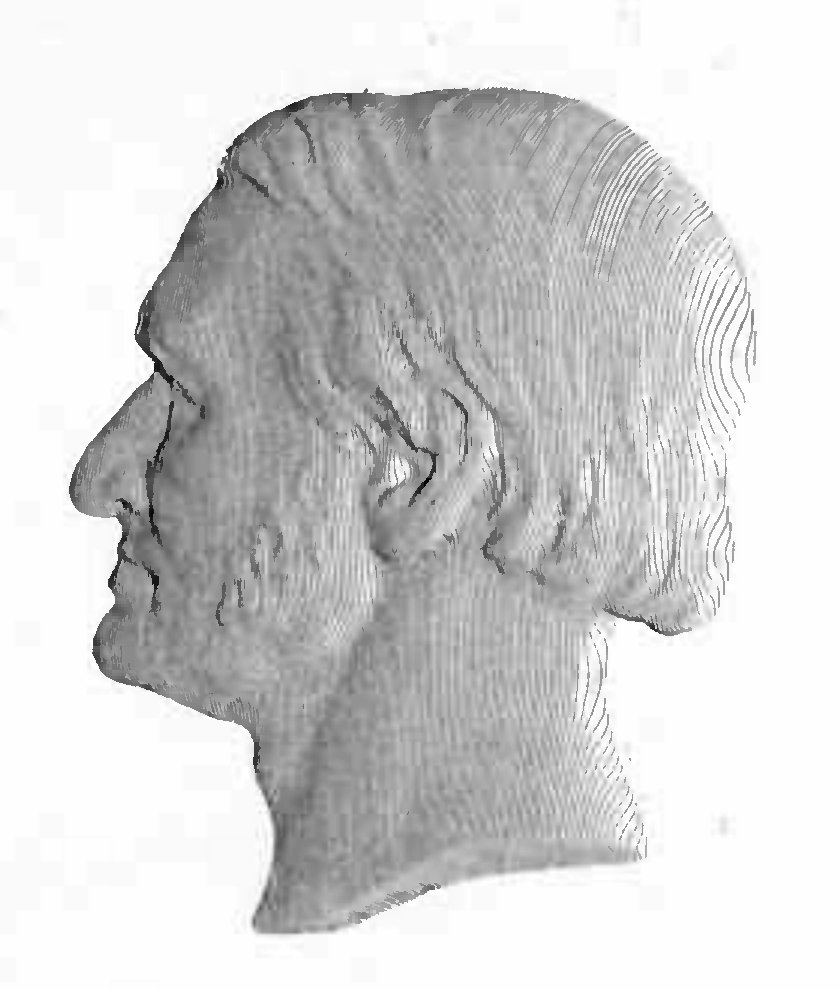
\includegraphics[width=1.6in]{assets/title_profile_contrast.png}\par
\vspace{.3in}{\large ZWEITER ABDRUCK\par}
\vspace{.2in}HERAUSGEGEBEN\par
\smallskip{\small VON DER\par}
\medskip{\small KÖNIGLICHEN GESELLSCHAFT DER WISSENSCHAFTEN\par}
\smallskip{\small ZU\par}
\medskip{\large GÖTTINGEN\par}
\smallskip1876.
\end{center}
\clearpage
\thispagestyle{empty}\SourceLeaf{11}
\pdfbookmark[0]{Theorematis arithmetici demonstratio nova}{paper-one-title}
\begin{center}
\vspace*{.8in}
{\Large THEOREMATIS ARITHMETICI\par}
\bigskip{\large DEMONSTRATIO NOVA\par}
\vspace{.6in}AUCTORE\par
\bigskip{\large CAROLO FRIDERICO GAUSS\par}
\vspace{.3in}{\small SOCIETATI REGIAE SCIENTIARUM TRADITA IAN. 15. 1808.\par}
\vspace{.65in}\rule{.85\linewidth}{.3pt}\par
\smallskip{\small Commentationes societatis regiae scientiarum Gottingensis. Vol. \textsc{xvi}.\par}
{\small Gottingae \textsc{mdcccviii}.\par}
\smallskip\rule{.85\linewidth}{.3pt}
\end{center}
\clearpage

\mainmatter
\SourceLeaf{13}%
% A544-P0013-O01
\begin{center}\Large THEOREMATIS ARITHMETICI\end{center}

% A544-P0013-O02
\begin{center}\large DEMONSTRATIO NOVA.\end{center}

% A544-P0013-O03
\BookRule{35mm}

% A544-P0013-O04
\Article{1}

% A544-P0013-O05
Quaestiones ex arithmetica sublimiori saepenumero phaenomenon singulare offerunt, quod in analysi longe rarius occurrit, atque ad illarum illecebras augendas multum confert.  Dum scilicet in disquisitionibus analyticis plerumque ad veritates novas pertingere non licet, nisi prius principiis, quibus innituntur, quaeque ad eas viam quasi patefacere debent, penitus potiti simus: contra in arithmetica frequentissime per inductionem fortuna quadam inopinata veritates elegantissimae novae prosiliunt, quarum demonstrationes tam profunde latent tantisque tenebris obvolutae sunt, ut omnes conatus eludant, acerrimisque perscrutationibus aditum denegent.  Tantus porro adest tamque mirus inter veritates arithmeticas, primo aspectu maxime heterogeneas, nexus, ut haud raro, dum longe alia quaerimus, tandem ad demonstrationem tantopere exoptatam longisque antea meditationibus frustra quaesitam longe alia via quam qua exspectata fuerat felicissime perveniamus.  Plerumque autem huiusmodi veritates eius sunt indolis, ut pluribus viis valde diversis adiri queant, nec semper viae brevissimae sint, quae primo se offerunt.  In magno itaque certe pretio habendum erit, si, tali veritate longe incassum ventilata, dein demonstrata quidem sed per ambages abstrusiores, tandem viam simplicissimam atque genuinam detegere contigerit.

% A544-P0013-O06
\Article{2}

% A544-P0013-O07
Inter quaestiones, de quibus in art. praec. diximus, locum insignem tenet theorema omnem fere theoriam residuorum quadraticorum continens, quod in \emph{Disquisitionibus arithmeticis} (Sect. IV.) \emph{theorematis fundamentalis} nomine distinctum \SourceLeaf{14}est.  Pro \emph{primo} huius elegantissimi theorematis inventore ill. \textsc{Legendre} absque dubio habendus est, postquam longe antea summi geometrae \textsc{Euler} et \textsc{Lagrange} plures eius casus speciales iam per inductionem detexerant.  Conatibus horum virorum circa demonstrationem enumerandis hic non immoror; adeant quibus volupe est opus modo commemoratum.  Adiicere liceat tantummodo, in confirmationem eorum, quae in art. praec. prolata sunt, quae ad meos conatus pertinent.  In ipsum theorema proprio marte incideram anno 1795, dum omnium, quae in arithmetica sublimiori iam elaborata fuerant, penitus ignarus et a subsidiis literariis omnino praeclusus essem: sed per integrum annum me torsit, operamque enixissimam effugit, donec tandem demonstrationem in Sectione quarta operis illius traditam nactus essem.  Postea tres aliae principiis prorsus diversis innixae se mihi obtulerunt, quarum unam in Sectione quinta tradidi, reliquas elegantia illa haud inferiores alia occasione publici iuris faciam.  Sed omnes hae demonstrationes, etiamsi respectu rigoris nihil desiderandum relinquere videantur, e principiis nimis heterogeneis derivatae sunt, prima forsan excepta, quae tamen per ratiocinia magis laboriosa procedit, operationibusque prolixioribus premitur.  Demonstrationem itaque \emph{genuinam} hactenus haud affuisse non dubito pronunciare: esto iam penes peritos iudicium, an ea, quam nuper detegere successit, quamque pagellae sequentes exhibent, hoc nomine decorari mereatur.

% A544-P0014-O03
\Article{3}

% A544-P0014-O04
\textsc{Theorema.}  \emph{Sit $p$ numerus primus positivus; $k$ integer quicunque per $p$ non} \emph{divisibilis;}

% A544-P0014-O05
\[
\begin{aligned}
A &\quad \text{\emph{complexus numerorum}}\quad 1,\ 2,\ 3\ \dotsfour\ \tfrac12(p-1)\\
B &\quad \text{\emph{complexus horum}}\quad \tfrac12(p+1),\ \tfrac12(p+3),\ \tfrac12(p+5)\ \dotsfour\ p-1
\end{aligned}
\]

% A544-P0014-O06
\emph{Capiantur residua minima positiva productorum ex $k$ in singulos numeros $A$ secundum modulum $p$, quae manifesto omnia diversa erunt, atque partim ad $A$ partim ad} \emph{$B$ pertinebunt.  Iam si ad $B$ omnino $\mu$ residua pertinere supponantur, erit $k$ vel residuum vel non-residuum quadraticum ipsius $p$, prout $\mu$ par est vel impar.}

% A544-P0014-O07
\emph{Dem.}  Sint residua ad $A$ pertinentia haec $a,\ a'\ a''\ \dotsfour$, reliqua ad $B$ pertinentia $b,b',b''\dotsfour$, patetque posteriorum complementa $p-b,p-b',p-b''\dotsfour$ cuncta a numeris $a,\ a',\ a''\ \dotsfour$ diversa esse, cum his vero simul sumta comple\SourceLeaf{15}xum $A$ explere.  Habemus itaque

% A544-P0015-O03
\[
\begin{aligned}
1\pdot2\pdot3\ \dotsfour\ \tfrac12(p-1)=aa' a''\ \dotsfour\ (p-b)(p-b')(p-b'')\ \dotsfour
\end{aligned}
\]

% A544-P0015-O04
Productum posterius autem manifesto fit

% A544-P0015-O05
\[
\begin{aligned}
&\equiv(-1)^\mu aa' a''\ \dotsfour\ bb' b''\ \dotsfour\ \equiv(-1)^\mu k\pdot2k\pdot3k\ \dotsfour\ \tfrac12(p-1)k\\
&\equiv(-1)^\mu k^{\frac12(p-1)}\,1\pdot2\pdot3\ \dotsfour\ \tfrac12(p-1) (\mathrm{mod.}p)
\end{aligned}
\]

% A544-P0015-O06
Hinc erit

% A544-P0015-O07
\[
\begin{aligned}
1\equiv(-1)^\mu k^{\frac12(p-1)}
\end{aligned}
\]

% A544-P0015-O08
sive $k^{\frac12(p-1)}\equiv\pm1$, prout $\mu$ par est vel impar, unde theorema nostrum protinus demanat.

% A544-P0015-O09
\Article{4}

% A544-P0015-O10
Ratiocinia sequentia magnopere abbreviare licebit per introductionem quarundam designationum idonearum.  Exprimet igitur nobis character $(k,p)$ multitudinem productorum ex his

% A544-P0015-O11
\[
\begin{aligned}
k,\ 2k,\ 3k\ \dotsfour\ \tfrac12(p-1)k,
\end{aligned}
\]

% A544-P0015-O12
quorum residua minima positiva secundum modulum $p$ huius semissem superant. Porro existente $x$ quantitate quacunque non integra, per signum $[x]$ exprimemus integrum ipsa $x$ proxime minorem, ita ut $x-[x]$ semper fiat quantitas positiva intra limites $0$ et $1$ sita.  Levi iam negotio relationes sequentes evolventur:

% A544-P0015-O13
I.  $[x]+[-x]=-1.$

% A544-P0015-O14
II.  $[x]+h=[x+h]$, quoties $h$ est integer.

% A544-P0015-O15
III.  $[x]+[h-x]=h-1.$

% A544-P0015-O16
IV.  Si $x-[x]$ est fractio minor quam $\tfrac12$, erit $[2x]-2[x]=0$; si vero $x-[x]$ est maior quam $\tfrac12$, erit $[2x]-2[x]=1.$

% A544-P0015-O17
V.  Iacente itaque residuo minimo positivo integri $h$ secundum modulum $p$ infra $\tfrac12p$, erit $\gbr{\frac{2h}{p}}-2\gbr{\frac{h}{p}}=0$; iacente autem residuo illo ultra $\tfrac12p$, erit $\gbr{\frac{2h}{p}}-2\gbr{\frac{h}{p}}=1.$

\SourceLeaf{16}%
% A544-P0016-O02
VI.  Hinc statim sequitur $(k,p)=$

% A544-P0016-O03
\[
\begin{aligned}
&\gbr{\frac{2k}{p}}+\gbr{\frac{4k}{p}}+\gbr{\frac{6k}{p}}\dotsfour+\gbr{\frac{(p-1)k}{p}}\\
&-2\gbr{\frac{k}{p}}-2\gbr{\frac{2k}{p}}-2\gbr{\frac{3k}{p}}\dotsfour-2\gbr{\frac{\frac12(p-1)k}{p}}.
\end{aligned}
\]

% A544-P0016-O04
VII.  Ex VI. et I. nullo negotio derivatur

% A544-P0016-O05
\[
\begin{aligned}
(k,p)+(-k,p)=\tfrac12(p-1)
\end{aligned}
\]

% A544-P0016-O06
Unde sequitur, $-k$ vel eandem vel oppositam relationem ad $p$ habere (quatenus huius residuum aut non-residuum quadraticum est) ut $+k$, prout $p$ vel formae $4n+1$ fuerit, vel formae $4n+3$.  In casu priori manifesto $-1$ residuum, in posteriori non-residuum ipsius $p$ erit.

% A544-P0016-O07
VIII.  Formulam in VI. traditam sequenti modo transformabimus. Per III. fit

% A544-P0016-O08
\[
\begin{aligned}
\gbr{\frac{(p-1)k}{p}}&=k-1-\gbr{\frac{k}{p}},\\
\gbr{\frac{(p-3)k}{p}}&=k-1-\gbr{\frac{3k}{p}},\\
\gbr{\frac{(p-5)k}{p}}&=k-1-\gbr{\frac{5k}{p}}\dotsfour
\end{aligned}
\]

% A544-P0016-O09
Applicando hasce substitutiones ad $\frac{p\mp1}{4}$ membra ultima seriei superioris in illa expressione, habebimus

% A544-P0016-O10
\Needspace{8\baselineskip}\emph{primo}, quoties $p$ est formae $4n+1$

% A544-P0016-O11
\[
\begin{aligned}
(k,p)&=\tfrac14(k-1)(p-1)\\
& -2\left\{\gbr{\frac{k}{p}}+\gbr{\frac{3k}{p}}+\gbr{\frac{5k}{p}}\dotsfour+\gbr{\frac{\frac12(p-3)k}{p}}\right\}\\
&\qquad-\left\{\gbr{\frac{k}{p}}+\gbr{\frac{2k}{p}}+\gbr{\frac{3k}{p}}\dotsfour+\gbr{\frac{\frac12(p-1)k}{p}}\right\}
\end{aligned}
\]

% A544-P0016-O12
\Needspace{8\baselineskip}\emph{secundo}, quoties $p$ est formae $4n+3$

% A544-P0016-O13
\[
\begin{aligned}
(k,p)&=\tfrac14(k-1)(p+1)\\
& -2\left\{\gbr{\frac{k}{p}}+\gbr{\frac{3k}{p}}+\gbr{\frac{5k}{p}}\dotsfour+\gbr{\frac{\frac12(p-1)k}{p}}\right\}\\
&\qquad-\left\{\gbr{\frac{k}{p}}+\gbr{\frac{2k}{p}}+\gbr{\frac{3k}{p}}\dotsfour+\gbr{\frac{\frac12(p-1)k}{p}}\right\}
\end{aligned}
\]

% A544-P0016-O14
IX.  Pro casu speciali $k=+2$ e formulis modo traditis sequitur $(2,p)=\tfrac14(p\mp1)$, sumendo signum superius vel inferius, prout $p$ est formae $4n+1$ vel $4n+3$.  Erit itaque $(2,p)$ par, adeoque $2Rp$, quoties $p$ est formae $8n+1$ vel $8n+7$; contra erit $(2,p)$ impar atque $2Np$, quoties $p$ est formae $8n+3$ vel $8n+5$.

\SourceLeaf{17}%
% A544-P0017-O02
\Article{5}

% A544-P0017-O03
\textsc{Theorema.}  \emph{Sit $x$ quantitas positiva non integra, inter cuius multipla $x$, $2x$,} \emph{$3x\dotsfour$ usque ad $nx$ nullum fiat integer; ponatur $[nx]=h$, unde facile concluditur,} \emph{etiam inter multipla quantitatis reciprocae $\frac1x$, $\frac2x$, $\frac3x\dotsfive$ usque ad $\frac hx$ integrum non} \emph{reperiri.  Tum dico fore}

% A544-P0017-O04
\[
\begin{aligned}
\left.\begin{aligned}
&[x]+[2x]+[3x]\dotstwo+[nx]\\
&+\gbr{\frac1x}+\gbr{\frac2x}+\gbr{\frac3x}\dotsfour+\gbr{\frac hx}
\end{aligned}\right\}=nh.
\end{aligned}
\]

% A544-P0017-O05
\emph{Dem.}  Seriei $[x]+[2x]+[3x]\dotsfour+[nx]$, quam ponemus $=\Omega$, membra prima usque ad $\gbr{\frac1x}^{\mathrm{tum}}$ inclus. manifesto omnia erunt $=0$; sequentia usque ad $\gbr{\frac2x}^{\mathrm{tum}}$ cuncta $=1$; sequentia usque ad $\gbr{\frac3x}^{\mathrm{tum}}$ cuncta $=2$ et sic porro. Hinc fit

% A544-P0017-O06
\[
\begin{aligned}
\left.\begin{aligned}
\Omega={}&0\times\gbr{\frac1x}\\
&+1\times\left\{\gbr{\frac2x}-\gbr{\frac1x}\right\}\\
&+2\times\left\{\gbr{\frac3x}-\gbr{\frac2x}\right\}\\
&+3\times\left\{\gbr{\frac4x}-\gbr{\frac3x}\right\}\\
&\hspace{12mm}\text{etc.}\\
&+(h-1)\left\{\gbr{\frac hx}-\gbr{\frac{h-1}{x}}\right\}\\
&+h\left\{n-\gbr{\frac hx}\right\}
\end{aligned}\right\}=hn-\gbr{\frac1x}-\gbr{\frac2x}-\gbr{\frac3x}\dotsfour-\gbr{\frac hx}
\end{aligned}
\]

% A544-P0017-O07
Q. E. D.

% A544-P0017-O08
\Article{6}

% A544-P0017-O09
\textsc{Theorema.}  \emph{Designantibus $k,p$ numeros positivos impares inter se primos quoscunque, erit}

% A544-P0017-O10
\[
\begin{aligned}
\left.\begin{aligned}
&\gbr{\frac kp}+\gbr{\frac{2k}{p}}+\gbr{\frac{3k}{p}}\dotsfour+\gbr{\frac{\frac12(p-1)k}{p}}\\
&+\gbr{\frac pk}+\gbr{\frac{2p}{k}}+\gbr{\frac{3p}{k}}\dotsfour+\gbr{\frac{\frac12(k-1)p}{k}}
\end{aligned}\right\}=\tfrac14(k-1)(p-1).
\end{aligned}
\]

% A544-P0017-O11
\emph{Demonstr.}  Supponendo, quod licet, $k<p$, erit $\frac{\frac12(p-1)k}{p}$ minor quam $\frac12 k$, sed maior quam $\frac12(k-1)$, adeoque $\gbr{\frac{\frac12(p-1)k}{p}}=\frac12(k-1)$.  Hinc patet, theorema praesens ex praec. protinus sequi, statuendo illic $\frac kp=x$, $\frac12(p-1)=n$, adeoque $\frac12(k-1)=h$.

\SourceLeaf{18}%
% A544-P0018-O02
Ceterum simili modo demonstrari potest, si $k$ fuerit numerus \emph{par} ad $p$ primus, fore

% A544-P0018-O03
\[
\begin{aligned}
\left.\begin{aligned}
&\gbr{\frac kp}+\gbr{\frac{2k}{p}}+\gbr{\frac{3k}{p}}\dotsfour+\gbr{\frac{\frac12(p-1)k}{p}}\\
&+\gbr{\frac pk}+\gbr{\frac{2p}{k}}+\gbr{\frac{3p}{k}}\dotsfour+\gbr{\frac{\frac12 kp}{k}}
\end{aligned}\right\}=\tfrac14 k(p-1)
\end{aligned}
\]

% A544-P0018-O04
At huic propositioni ad institutum nostrum non necessariae non immoramur.

% A544-P0018-O05
\Article{7}

% A544-P0018-O06
Iam ex combinatione theorematis praec. cum propos. VIII. art. 4. theorema fundamentale protinus demanat.  Nimirum denotantibus $k,p$ numeros primos positivos inaequales quoscunque, et ponendo

% A544-P0018-O07
\[
\begin{aligned}
(k,p)+\gbr{\frac kp}+\gbr{\frac{2k}{p}}+\gbr{\frac{3k}{p}}\dotsfour+\gbr{\frac{\frac12(p-1)k}{p}}&=L\\
(p,k)+\gbr{\frac pk}+\gbr{\frac{2p}{k}}+\gbr{\frac{3p}{k}}\dotsfour+\gbr{\frac{\frac12(k-1)p}{k}}&=M
\end{aligned}
\]

% A544-P0018-O08
per VIII. art. 4. patet, $L$ et $M$ semper fieri numeros pares.  At per theorema art. 6. erit

% A544-P0018-O09
\[
\begin{aligned}
L+M=(k,p)+(p,k)+\tfrac14(k-1)(p-1)
\end{aligned}
\]

% A544-P0018-O10
Quoties igitur $\frac14(k-1)(p-1)$ par evadit, quod fit, si vel uterque $k,p$ vel saltem alteruter est formae $4n+1$, necessario $(k,p)$ et $(p,k)$ vel ambo pares vel ambo impares esse debent.  Quoties autem $\frac14(k-1)(p-1)$ impar est, quod evenit, si uterque $k,p$ est formae $4n+3$, necessario alter numerorum $(k,p)$, $(p,k)$ par, alter impar esse debebit.  In casu priori itaque relatio ipsius $k$ ad $p$ et relatio ipsius $p$ ad $k$ (quatenus alter alterius residuum vel non-residuum est) identicae erunt, in casu posteriori oppositae.

% A544-P0018-O11
Q. E. D.

% A544-P0018-O12
\BookRule{35mm}


\clearpage\thispagestyle{empty}\SourceLeaf{19}
\pdfbookmark[0]{Summatio quarumdam serierum singularium}{paper-two-title}
\begin{center}
\vspace*{.6in}{\large SUMMATIO\par}
\bigskip{\Large QUARUMDAM SERIERUM\par}
\bigskip{\large SINGULARIUM\par}
\vspace{.65in}AUCTORE\par
\bigskip{\large CAROLO FRIDERICO GAUSS\par}
\vspace{.3in}{\small EXHIBITA SOCIETATI D. XXIV. AUGUST. MDCCCVIII.\par}
\vspace{.6in}\rule{.85\linewidth}{.3pt}\par
\smallskip{\small Commentationes societatis regiae scientiarum Gottingensis recentiores. Vol. \textsc{i}.\par}
{\small Gottingae \textsc{mdcccxi}.\par}
\smallskip\rule{.85\linewidth}{.3pt}
\end{center}

\clearpage
\renewcommand{\BookRunningTitle}{Summatio quarumdam serierum singularium}
\renewcommand{\Article}[1]{\par\medskip\Needspace{4\baselineskip}\pdfbookmark[1]{Art. #1}{paper-two-art-#1}\centerline{\textbf{#1.}}\nobreak\smallskip}
\SourceLeaf{21}%
% A544-P0021-O01
\begin{center}\Large SUMMATIO\end{center}

% A544-P0021-O02
\begin{center}\large QUARUMDAM SERIERUM SINGULARIUM.\end{center}

% A544-P0021-O03
\BookRule{22mm}

% A544-P0021-O04
\Article{1}

% A544-P0021-O05
Inter veritates insigniores, ad quas theoria divisionis circuli aditum aperuit, locum haud ultimum sibi vindicat summatio in Disquiss. Arithmet. art. 356 proposita, non modo propter elegantiam suam peculiarem, miramque foecunditatem, quam fusius exponendi occasionem posthac dabit alia disquisitio, sed ideo quoque, quod eius demonstratio rigorosa atque completa difficultatibus haud vulgaribus premitur.\quad Quae sane eo minus exspectari debuissent, quum non tam in ipsum theorema cadant, quam potius in aliquam theorematis limitationem, qua neglecta demonstratio statim in promtu est, facillimeque e theoria in opere isto explicata derivatur.\quad Theorema illic exhibitum est in forma sequente.\quad Supponendo $n$ esse numerum primum, denotandoque indefinite omnia residua quadratica ipsius $n$ inter limites $1$ et $n-1$ incl. sita per $a$, omniaque non-residua inter eosdem limites iacentia per $b$, denique per $\omega$ arcum $\frac{360^{0}}{n}$, et per $k$ integrum determinatum quemcunque per $n$ non divisibilem, erit

% A544-P0021-O06
I.\quad pro valore ipsius $n$, qui est formae $4m+1$,

% A544-P0021-O07
\[
\begin{aligned}
\Sigma\cos ak\omega&=-\tfrac12\pm\tfrac12\surd n\\
\Sigma\cos bk\omega&=-\tfrac12\mp\tfrac12\surd n,\ \text{adeoque}\\
\Sigma\cos ak\omega-\Sigma\cos bk\omega&=\pm\surd n\\
\Sigma\sin ak\omega&=0\\
\Sigma\sin bk\omega&=0
\end{aligned}
\]

\SourceLeaf{22}%
% A544-P0022-RC02
II.\quad pro valore ipsius $n$, qui est formae $4m+3$,

% A544-P0022-RC03
\[
\begin{aligned}
\Sigma\cos ak\omega&=-\tfrac12\\
\Sigma\cos bk\omega&=-\tfrac12\\
\Sigma\sin ak\omega&=\pm\tfrac12\surd n\\
\Sigma\sin bk\omega&=\mp\tfrac12\surd n\\
\Sigma\sin ak\omega-\Sigma\sin bk\omega&=\pm\surd n
\end{aligned}
\]

% A544-P0022-RC04
Hae summationes l. c. omni rigore demonstratae sunt, neque alia difficultas hic remanet nisi in determinatione \emph{signi} quantitati radicali praefigendi.\quad Nullo quidem negotio ostendi potest, hoc signum eatenus a numero $k$ pendere, quod semper pro cunctis valoribus ipsius $k$, qui sint residua quadratica ipsius $n$, signum \emph{idem} valere debeat, et contra signum huic oppositum pro omnibus valoribus ipsius $k$, qui sint non-residua quadratica ipsius $n$.\quad Hinc totum negotium in valore $k=1$ versabitur, patetque, quam primum signum pro hoc valore valens innotuerit, pro omnibus quoque reliquis valoribus ipsius $k$ signa statim in promtu fore.\quad Verum enim vero in hac ipsa quaestione, quae primo aspectu inter faciliores referenda videtur, in difficultates improvisas incidimus, methodusque, qua ducente sine impedimentis hucusque progressi eramus, auxilium ulterius prorsus denegat.

% A544-P0022-RC05
\Article{2}

% A544-P0022-RC06
Haud abs re erit, antequam ulterius progrediamur, quaedam exempla summationis nostrae per calculum numericum evolvisse: huic vero quasdam observationes generales praemittere conveniet.

% A544-P0022-RC07
I.\quad Si in casu eo, ubi $n$ est numerus primus formae $4m+1$, omnia residua quadratica ipsius $n$ inter $1$ et $\frac12(n-1)$ incl. iacentia indefinite per $a'$ exhibentur, omniaque non-residua inter eosdem limites per $b'$ constat, omnes $n-a'$ inter ipsos $a$, omnesque $n-b'$ inter $b$ comprehensos fore: quamobrem quum omnes $a'$, $b'$, $n-a'$, $n-b'$ manifesto totum complexum numerorum $1$, $2$, $3\dotsfour$ $n-1$ expleant, omnes $a'$ cum omnibus $n-a'$ iuncti omnes $a$ complectentur, et perinde omnes $b'$ cum omnibus $n-b'$ iuncti omnes $b$ comprehendent.\quad Hinc erit

\SourceLeaf{23}%
% A544-P0023-RC02
\[
\begin{aligned}
\Sigma\cos ak\omega&=\Sigma\cos a'k\omega+\Sigma\cos(n-a')k\omega\\
\Sigma\cos bk\omega&=\Sigma\cos b'k\omega+\Sigma\cos(n-b')k\omega\\
\Sigma\sin ak\omega&=\Sigma\sin a'k\omega+\Sigma\sin(n-a')k\omega\\
\Sigma\sin bk\omega&=\Sigma\sin b'k\omega+\Sigma\sin(n-b')k\omega
\end{aligned}
\]

% A544-P0023-RC03
Iam quum habeatur $\cos(n-a')k\omega=\cos a'k\omega$, $\cos(n-b')k\omega=\cos b'k\omega$, $\sin(n-a')k\omega=-\sin a'k\omega$, $\sin(n-b')k\omega=-\sin b'k\omega$, patet sponte fieri

% A544-P0023-RC04
\[
\begin{aligned}
\Sigma\sin ak\omega&=\Sigma\sin a'k\omega-\Sigma\sin a'k\omega=0\\
\Sigma\sin bk\omega&=\Sigma\sin b'k\omega-\Sigma\sin b'k\omega=0
\end{aligned}
\]

% A544-P0023-RC05
Summatio cosinuum vero hanc formam assumit

% A544-P0023-RC06
\[
\begin{aligned}
\Sigma\cos ak\omega&=2\Sigma\cos a'k\omega\\
\Sigma\cos bk\omega&=2\Sigma\cos b'k\omega
\end{aligned}
\]

% A544-P0023-RC07
unde fieri debebit

% A544-P0023-RC08
\[
\begin{aligned}
1+4\Sigma\cos a'k\omega&=\pm\surd n\\
1+4\Sigma\cos b'k\omega&=\mp\surd n\\
2\Sigma\cos a'k\omega-2\Sigma\cos b'k\omega&=\pm\surd n
\end{aligned}
\]

% A544-P0023-RC09
II.\quad In casu eo, ubi $n$ est formae $4m+3$, complementum cuiusvis residui $a$ ad $n$ erit non-residuum, complementumque cuiusvis $b$ erit residuum; quocirca omnes $n-a$ convenient cum omnibus $b$, omnesque $n-b$ cum omnibus $a$. Hinc colligitur

% A544-P0023-RC10
\[
\begin{aligned}
\Sigma\cos ak\omega=\Sigma\cos(n-b)k\omega=\Sigma\cos bk\omega
\end{aligned}
\]

% A544-P0023-RC11
quare quum omnes $a$ et $b$ iuncti omnes numeros $1$, $2$, $3\dotsfour n-1$ expleant, adeoque fiat $\Sigma\cos ak\omega+\Sigma\cos bk\omega=\cos k\omega+\cos2k\omega+\cos3k\omega+\text{etc.}$ $+\cos(n-1)k\omega=-1$, summationes

% A544-P0023-RC12
\[
\begin{aligned}
\Sigma\cos ak\omega&=-\tfrac12\\
\Sigma\cos bk\omega&=-\tfrac12
\end{aligned}
\]

% A544-P0023-RC13
sponte sunt obviae.\quad Perinde erit

% A544-P0023-RC14
\[
\begin{aligned}
\Sigma\sin ak\omega=\Sigma\sin(n-b)k\omega=-\Sigma\sin bk\omega
\end{aligned}
\]

\SourceLeaf{24}%
% A544-P0024-RC02
unde patet, quomodo summationum

% A544-P0024-RC03
\[
\begin{aligned}
2\Sigma\sin ak\omega&=\pm\surd n\\
2\Sigma\sin bk\omega&=\mp\surd n
\end{aligned}
\]

% A544-P0024-RC04
altera ab altera pendeat.

% A544-P0024-RC05
\Article{3}

% A544-P0024-RC06
Ecce iam computum numericum pro aliquot exemplis:

% A544-P0024-RC07
I.\quad Pro $n=5$ adest valor unus ipsius $a'$, puta $a'=1$, valorque unus ipsius $b'$, puta $b'=2$; est autem

% A544-P0024-RC08
\[
\begin{aligned}
\cos\omega=+0{,}3090169944\qquad\cos2\omega=-0{,}8090169944
\end{aligned}
\]

% A544-P0024-RC09
adeoque $1+4\cos\omega=+\surd5$,\quad $1+4\cos2\omega=-\surd5$.

% A544-P0024-RC10
II.\quad Pro $n=13$ adsunt tres valores ipsius $a'$, puta $1$, $3$, $4$, totidemque valores ipsius $b'$, puta $2$, $5$, $6$, unde computamus

% A544-P0024-RC11
{\small\setlength{\arraycolsep}{2.5pt}\renewcommand{\arraystretch}{1.15}
\[
\begin{array}{rclcrcl}
\cos\omega&=&+0{,}8854560257&\qquad&\cos2\omega&=&+0{,}5680647467\\
\cos3\omega&=&+0{,}1205366803&\qquad&\cos5\omega&=&-0{,}7485107482\\
\cos4\omega&=&-0{,}3546048870&\qquad&\cos6\omega&=&-0{,}9709418174\\\cline{1-3}\cline{5-7}
\text{Summa}&=&+0{,}6513878190&\qquad&\text{Summa}&=&-1{,}1513878189
\end{array}
\]
}

% A544-P0024-RC12
Hinc $1+4\Sigma\cos a'\omega=+\surd13$,\quad $1+4\Sigma\cos b'\omega=-\surd13$.

% A544-P0024-RC13
III.\quad Pro $n=17$ habemus quatuor valores ipsius $a'$, puta $1$, $2$, $4$, $8$, totidemque valores ipsius $b'$, puta $3$, $5$, $6$, $7$.\quad Hinc computantur cosinus

% A544-P0024-RC14
{\small\setlength{\arraycolsep}{2.5pt}\renewcommand{\arraystretch}{1.15}
\[
\begin{array}{rclcrcl}
\cos\omega&=&+0{,}9324722294&\qquad&\cos3\omega&=&+0{,}4457383558\\
\cos2\omega&=&+0{,}7390089172&\qquad&\cos5\omega&=&-0{,}2736629901\\
\cos4\omega&=&+0{,}0922683595&\qquad&\cos6\omega&=&-0{,}6026346364\\
\cos8\omega&=&-0{,}9829730997&\qquad&\cos7\omega&=&-0{,}8502171357\\\cline{1-3}\cline{5-7}
\text{Summa}&=&+0{,}7807764064&\qquad&\text{Summa}&=&-1{,}2807764065
\end{array}
\]
}

% A544-P0024-RC15
Hinc $1+4\Sigma\cos a'\omega=+\surd17$,\quad $1+4\Sigma\cos b'\omega=-\surd17$.

\SourceLeaf{25}%
% A544-P0025-RC02
IV.\quad Pro $n=3$ adest valor unicus ipsius $a$, puta $a=1$, cui respondet

% A544-P0025-RC03
\[
\begin{aligned}
\sin\omega=+0{,}8660254038
\end{aligned}
\]

% A544-P0025-RC04
Hinc $2\sin\omega=+\surd3$.

% A544-P0025-RC05
V.\quad Pro $n=7$ adsunt valores tres ipsius $a$, puta $1$, $2$, $4$: hinc habentur sinus

% A544-P0025-RC06
{\small\setlength{\arraycolsep}{2.5pt}\renewcommand{\arraystretch}{1.15}
\[
\begin{array}{rcll}
\sin\omega&=&+0{,}7818314825&\\
\sin2\omega&=&+0{,}9749279122&\\
\sin4\omega&=&-0{,}4338837391&\\\cline{1-3}
\text{Summa}&=&+1{,}3228756556,&\text{adeoque }2\Sigma\sin a\omega=+\surd7.
\end{array}
\]
}

% A544-P0025-RC07
VI.\quad Pro $n=11$ valores ipsius $a$ sunt $1$, $3$, $4$, $5$, $9$, quibus respondent sinus

% A544-P0025-RC08
{\small\setlength{\arraycolsep}{2.5pt}\renewcommand{\arraystretch}{1.15}
\[
\begin{array}{rcll}
\sin\omega&=&+0{,}5406408175&\\
\sin3\omega&=&+0{,}9898214419&\\
\sin4\omega&=&+0{,}7557495744&\\
\sin5\omega&=&+0{,}2817325568&\\
\sin9\omega&=&-0{,}9096319954&\\\cline{1-3}
\text{Summa}&=&+1{,}6583123952,&\text{et proin }2\Sigma\sin a\omega=+\surd11.
\end{array}
\]
}

% A544-P0025-RC09
VII.\quad Pro $n=19$ valores ipsius $a$ sunt $1$, $4$, $5$, $6$, $7$, $9$, $11$, $16$, $17$, quibus respondent sinus

% A544-P0025-RC10
{\small\setlength{\arraycolsep}{2.5pt}\renewcommand{\arraystretch}{1.15}
\[
\begin{array}{rcll}
\sin\omega&=&+0{,}3246994692&\\
\sin4\omega&=&+0{,}9694002659&\\
\sin5\omega&=&+0{,}9965844930&\\
\sin6\omega&=&+0{,}9157733267&\\
\sin7\omega&=&+0{,}7357239107&\\
\sin9\omega&=&+0{,}1645945903&\\
\sin11\omega&=&-0{,}4759473930&\\
\sin16\omega&=&-0{,}8371664783&\\
\sin17\omega&=&-0{,}6142127127&\\\cline{1-3}
\text{Summa}&=&+2{,}1794494718,&\text{adeoque }2\Sigma\sin a\omega=+\surd19.
\end{array}
\]
}

\SourceLeaf{26}%
% A544-P0026-RC02
\Article{4}

% A544-P0026-RC03
In omnibus hisce exemplis quantitas radicalis signum positivum obtinet, idemque facile pro valoribus maioribus $n=23$, $n=29$ etc. confirmatur, unde fortis iam probabilitas oritur, hoc generaliter perinde se habere.\quad Sed demonstratio huius phaenomeni e principiis l. c. expositis peti nequit, plenissimoque iure altioris indaginis aestimanda est.\quad Propositum itaque huius commentationes eo tendit, ut demonstrationem rigorosam huius elegantissimi theorematis, per plures annos olim variis modis incassum tentatam, tandemque per considerationes singulares satisque subtiles feliciter perfectam in medium proferamus, simulque theorema ipsum salva seu potius aucta elegantia sua ad longe maiorem generalitatem evehamus.\quad Coronidis denique loco nexum mirabilem arctissimum inter hanc summationem aliudque theorema arithmeticum gravissimum docebimus.\quad Speramus, hasce disquisitiones non modo per se geometris gratas fore, sed methodos quoque, per quas haec omnia efficere licuit, quaeque in aliis quoque occasionibus utiles esse poterunt, ipsorum attentione dignas visum iri.

% A544-P0026-RC04
\Article{5}

% A544-P0026-RC05
Petita est demonstratio nostra e consideratione generis singularis progressionum, quarum termini pendent ab expressionibus talibus

% A544-P0026-RC06
\[
\begin{aligned}
\frac{(1-x^m)\,(1-x^{m-1})\,(1-x^{m-2})\dotsfour(1-x^{m-\mu+1})}{(1-x)\,(1-xx)\,(1-x^3)\dotsfive(1-x^\mu)}
\end{aligned}
\]

% A544-P0026-RC07
Brevitatis caussa talem fractionem per $(m,\mu)$ denotabimus, et primo quasdam observationes generales circa huiusmodi functiones praemittemus.

% A544-P0026-RC08
I.\quad Quoties $m$ est integer positivus minor quam $\mu$, functio $(m,\mu)$ manifesto evanescit, numeratore factorem $1-x^0$ implicante.\quad Pro $m=\mu$, factores in numeratore identici erunt ordine inverso cum factoribus in denominatore, unde erit $(\mu,\mu)=1$: denique pro casu eo, ubi $m$ est integer positivus maior quam $\mu$, habentur formulae

% A544-P0026-RC09
\[
\begin{aligned}
(\mu+1,\mu)&=\frac{1-x^{\mu+1}}{1-x}=(\mu+1,1)\\
(\mu+2,\mu)&=\frac{(1-x^{\mu+2})\,(1-x^{\mu+1})}{(1-x)\qquad(1-xx)}=(\mu+2,2)\\
(\mu+3,\mu)&=\frac{(1-x^{\mu+3})(1-x^{\mu+2})(1-x^{\mu+1})}{(1-x)\qquad(1-xx)\qquad(1-x^3)}=(\mu+3,3)\ \text{etc.}
\end{aligned}
\]

\SourceLeaf{27}%
% A544-P0027-RC02
sive generaliter

% A544-P0027-RC03
\[
\begin{aligned}
(m,\mu)=(m,m-\mu)
\end{aligned}
\]

% A544-P0027-RC04
II.\quad Porro facile confirmatur, haberi generaliter

% A544-P0027-RC05
\[
\begin{aligned}
(m,\mu+1)=(m-1,\mu+1)+x^{m-\mu-1}(m-1,\mu)
\end{aligned}
\]

% A544-P0027-RC06
quamobrem, quum perinde sit

% A544-P0027-RC07
\[
\begin{aligned}
(m-1,\mu+1)&=(m-2,\mu+1)+x^{m-\mu-2}(m-2,\mu)\\
(m-2,\mu+1)&=(m-3,\mu+1)+x^{m-\mu-3}(m-3,\mu)\\
(m-3,\mu+1)&=(m-4,\mu+1)+x^{m-\mu-4}(m-4,\mu),\ \text{etc.}
\end{aligned}
\]

% A544-P0027-RC08
quae series continuari poterit usque ad

% A544-P0027-RC09
\[
\begin{aligned}
(\mu+2,\mu+1)&=(\mu+1,\mu+1)+x(\mu+1,\mu)\\
&=(\mu,\mu)+x(\mu+1,\mu)
\end{aligned}
\]

% A544-P0027-RC10
siquidem $m$ est integer positivus maior quam $\mu+1$, erit

% A544-P0027-RC11
\[
\begin{aligned}
(m,\mu+1)&=(\mu,\mu)+x(\mu+1,\mu)+xx(\mu+2,\mu)\\
&\qquad+x^3(\mu+3,\mu)+\text{etc.}\\
&\qquad+x^{m-\mu-1}(m-1,\mu)
\end{aligned}
\]

% A544-P0027-RC12
Hinc patet, si pro aliquo valore determinato ipsius $\mu$ quaevis functio $(m,\mu)$ integra sit, existente $m$ integro positivo, etiam quamvis functionem $(m,\mu+1)$ integram evadere debere.\quad Quare quum suppositio illa pro $\mu=1$ locum habeat, eadem etiam pro $\mu=2$ valebit, atque hinc etiam pro $\mu=3$ etc., i. e. generaliter pro valore quocunque integro positivo ipsius $m$ erit $(m,\mu)$ functio integra. sive productum

% A544-P0027-RC13
\[
\begin{aligned}
(1-x^m)(1-x^{m-1})(1-x^{m-2})\dotsfour(1-x^{m-\mu+1})
\end{aligned}
\]

% A544-P0027-RC14
divisibile per

% A544-P0027-RC15
\[
\begin{aligned}
(1-x)(1-x^2)(1-x^3)\dotsfour(1-x^\mu)
\end{aligned}
\]

% A544-P0027-RC16
\Article{6}

% A544-P0027-RC17
Duas iam progressiones considerabimus, quae ambae ad scopum nostrum ducere possunt.\quad Progressio prima haec est

\SourceLeaf{28}%
% A544-P0028-RC02
\[
\begin{aligned}
&1-\frac{1-x^m}{1-x}+\frac{(1-x^m)\,(1-x^{m-1})}{(1-x)\,(1-xx)}\\
&\qquad-\frac{(1-x^m)(1-x^{m-1})(1-x^{m-2})}{(1-x)\quad(1-xx)\quad(1-x^3)}+\text{etc.}
\end{aligned}
\]

% A544-P0028-RC03
sive

% A544-P0028-RC04
\[
\begin{aligned}
1-(m,1)+(m,2)-(m,3)+(m,4)-\text{etc.}
\end{aligned}
\]

% A544-P0028-RC05
quam brevitatis caussa per $f(x,m)$ denotabimus.\quad Primo statim obvium est, quoties $m$ sit numerus integer positivus, hanc seriem post terminum suum $m+1^{\mathrm{tum}}$ (qui fit $=\pm1$) \emph{abrumpi}, adeoque in hoc casu summam fieri debere functionem finitam integram ipsius $x$.\quad Porro per art. 5. II. patet, generaliter pro valore quocunque ipsius $m$ haberi

% A544-P0028-RC06
\[
\begin{aligned}
1&=1\\
-(m,1)&=-(m-1,1)-x^{m-1}\\
+(m,2)&=+(m-1,2)+x^{m-2}(m-1,1)\\
-(m,3)&=-(m-1,3)-x^{m-3}(m-1,2),\ \text{etc.}
\end{aligned}
\]

% A544-P0028-RC07
adeoque

% A544-P0028-RC08
\[
\begin{aligned}
f(x,m)&=1-x^{m-1}-(1-x^{m-2})(m-1,1)\\
&\qquad+(1-x^{m-3})(m-1,2)\\
&\qquad-(1-x^{m-4})(m-1,3)+\text{etc.}
\end{aligned}
\]

% A544-P0028-RC09
Sed manifesto fit

% A544-P0028-RC10
\[
\begin{aligned}
(1-x^{m-2})(m-1,1)&=(1-x^{m-1})(m-2,1)\\
(1-x^{m-3})(m-1,2)&=(1-x^{m-1})(m-2,2)\\
(1-x^{m-4})(m-1,3)&=(1-x^{m-1})(m-2,3),\ \text{etc.}
\end{aligned}
\]

% A544-P0028-RC11
unde deducimus aequationem

% A544-P0028-RC12
\[
\begin{aligned}
f(x,m)=(1-x^{m-1})f(x,m-2)\ .\ .\ .\ .\ .\ .\ .\ .\ [1]
\end{aligned}
\]

% A544-P0028-RC13
\Article{7}

% A544-P0028-RC14
Quum pro $m=0$ fiat $f(x,m)=1$, per formulam modo inventam erit

% A544-P0028-RC15
\[
\begin{aligned}
f(x,2)&=1-x\\
f(x,4)&=(1-x)(1-x^3)\\
f(x,6)&=(1-x)(1-x^3)(1-x^5)\\
f(x,8)&=(1-x)(1-x^3)(1-x^5)(1-x^7),\ \text{etc.}
\end{aligned}
\]

% A544-P0028-RC16
sive generaliter pro valore quocunque pari ipsius $m$

% A544-P0028-RC17
\[
\begin{aligned}
f(x,m)=(1-x)(1-x^3)(1-x^5)\dotsfour(1-x^{m-1})\ .\ .\ .\ [2].
\end{aligned}
\]

\SourceLeaf{29}%
% A544-P0029-RC02
Contra quum pro $m=1$ fiat $f(x,m)=0$, erit etiam

% A544-P0029-RC03
\[
\begin{aligned}
f(x,3)&=0\\
f(x,5)&=0\\
f(x,7)&=0\ \text{etc.}
\end{aligned}
\]

% A544-P0029-RC04
sive generaliter pro valore quocunque impari ipsius $m$

% A544-P0029-RC05
\[
\begin{aligned}
f(x,m)=0
\end{aligned}
\]

% A544-P0029-RC06
Ceterum summatio posterior iam inde derivari potuisset, quod in progressione

% A544-P0029-RC07
\[
\begin{aligned}
1-(m,1)+(m,2)-(m,3)+\text{etc.}+(m,m-1)-(m,m)
\end{aligned}
\]

% A544-P0029-RC08
terminus ultimus primum destruit, penultimus secundum etc.

% A544-P0029-RC09
\Article{8}

% A544-P0029-RC10
Ad scopum quidem nostrum sufficit casus is, ubi $m$ est integer positivus impar: sed propter rei singularitatem etiam de casibus iis, ubi $m$ vel fractus vel negativus est, pauca adiecisse haud poenitebit.\quad Manifesto tunc series nostra haud amplius abrumpetur, sed in infinitum excurret, facileque insuper perspicitur, divergentem eam fieri, quoties ipsi $x$ valor minor quam $1$ tribuatur, quapropter ipsius summatio ad valores ipsius $x$ qui sint maiores quam $1$ restringi debebit.

% A544-P0029-RC11
Per formulam [1] art. 6. habemus

% A544-P0029-RC12
\[
\begin{aligned}
f(x,-2)&=\frac{1}{1-\frac1x}\\[8pt]
f(x,-4)&=\frac{1}{1-\frac1x}\pdot\frac{1}{1-\frac1{x^3}}\\[8pt]
f(x,-6)&=\frac{1}{1-\frac1x}\pdot\frac{1}{1-\frac1{x^3}}\pdot\frac{1}{1-\frac1{x^5}},\ \text{etc.}
\end{aligned}
\]

% A544-P0029-RC13
ita ut valor functionis $f(x,m)$ etiam pro valore negativo integro pari ipsius $m$ in terminis finitis assignabilis sit.\quad Pro reliquis vero valoribus ipsius $m$ functionem $f(x,m)$ in \emph{productum infinitum} sequenti modo convertemus.

% A544-P0029-RC14
Crescente $m$ in valorem negativum \emph{infinitum}, functio $f(x,m)$ transit in

\SourceLeaf{30}%
% A544-P0030-B02
\[
\begin{aligned}
&1+\frac1{x-1}+\frac1{x-1}\pdot\frac1{xx-1}\\
&\qquad+\frac1{x-1}\pdot\frac1{xx-1}\pdot\frac1{x^3-1}+\text{etc.}
\end{aligned}
\]

% A544-P0030-B03
Haec itaque series aequalis est producto infinito

% A544-P0030-B04
\[
\begin{aligned}
\frac1{1-\frac1x}\pdot\frac1{1-\frac1{x^3}}\pdot\frac1{1-\frac1{x^5}}\pdot\frac1{1-\frac1{x^7}}\;\text{etc. in infin.}
\end{aligned}
\]

% A544-P0030-B05
Porro quum generaliter sit

% A544-P0030-B06
\[
\begin{aligned}
f(x,m)&=f(x,m-2\lambda)\pdot(1-x^{m-1})(1-x^{m-3})\\
&\qquad(1-x^{m-5})\dotstwo(1-x^{m-2\lambda+1})
\end{aligned}
\]

% A544-P0030-B07
erit

% A544-P0030-B08
\[
\begin{aligned}
f(x,m)&=f(x,-\infty)\pdot(1-x^{m-1})(1-x^{m-3})(1-x^{m-5})\\
&\qquad\text{etc. in infin.}\\
&=\frac{1-x^{m-1}}{1-x^{-1}}\pdot\frac{1-x^{m-3}}{1-x^{-3}}\pdot\frac{1-x^{m-5}}{1-x^{-5}}\pdot\frac{1-x^{m-7}}{1-x^{-7}}\\
&\qquad\text{etc. in infin.}
\end{aligned}
\]

% A544-P0030-B09
quos factores tandem continuo magis ad unitatem convergere palam est.

% A544-P0030-B10
Attentionem peculiarem meretur casus $m=-1$, ubi fit

% A544-P0030-B11
\[
\begin{aligned}
f(x,-1)=1+x^{-1}+x^{-3}+x^{-6}+x^{-10}+\text{etc.}
\end{aligned}
\]

% A544-P0030-B12
Haec itaque series aequatur producto infinito

% A544-P0030-B13
\[
\begin{aligned}
\frac{1-x^{-2}}{1-x^{-1}}\pdot\frac{1-x^{-4}}{1-x^{-3}}\pdot\frac{1-x^{-6}}{1-x^{-5}}\;\text{etc.}
\end{aligned}
\]

% A544-P0030-B14
sive scribendo $x$ pro $x^{-1}$, erit

% A544-P0030-B15
\[
\begin{aligned}
1+x+x^3+x^6+\text{etc.}&=\frac{1-xx}{1-x}\pdot\frac{1-x^4}{1-x^3}\pdot\frac{1-x^6}{1-x^5}\\
&\qquad\pdot\frac{1-x^8}{1-x^7}\;\text{etc.}
\end{aligned}
\]

% A544-P0030-B16
Haec aequalitas inter duas expressiones abstrusiores, ad quas alia occasione reveniemus, valde sane est memorabilis.

% A544-P0030-B17
\Article{9}

% A544-P0030-B18
Secundo loco considerabimus progressionem hancce

% A544-P0030-B19
\[
\begin{aligned}
&1+x^{\frac12}\frac{1-x^m}{1-x}+x\frac{(1-x^m)(1-x^{m-1})}{(1-x)(1-xx)}\\
&\qquad+x^{\frac32}\frac{(1-x^m)(1-x^{m-1})(1-x^{m-2})}{(1-x)(1-xx)(1-x^3)}+\text{etc.}
\end{aligned}
\]

% A544-P0030-B20
sive

% A544-P0030-B21
\[
\begin{aligned}
1+x^{\frac12}(m,1)+x(m,2)+x^{\frac32}(m,3)+xx(m,4)+\text{etc.}
\end{aligned}
\]

% A544-P0030-B22
quam per $F(x,m)$ denotabimus.\quad Restringemus hanc disquisitionem ad casum eum, ubi $m$ est integer positivus, ita ut haec quoque series semper abrumpatur %

\SourceLeaf{31}%
% A544-P0031-B02
cum termino $m+1^{\mathrm{to}}$, qui est $=x^{\frac12m}(m,m)$.\quad Quum sit.

% A544-P0031-B03
\[
\begin{aligned}
(m,m)=1,\quad(m,m-1)=(m,1),\quad(m,m-2)=(m,2),\;\text{etc.}
\end{aligned}
\]

% A544-P0031-B04
progressio ita quoque exhiberi poterit:

% A544-P0031-B05
\[
\begin{aligned}
F(x,m)&=x^{\frac12m}+x^{\frac12(m-1)}(m,1)\\&\qquad+x^{\frac12(m-2)}(m,2)+x^{\frac12(m-3)}(m,3)+\text{etc.}
\end{aligned}
\]

% A544-P0031-B06
Hinc fit

% A544-P0031-B07
\[
\begin{aligned}
(1+x^{\frac12m+\frac12})F(x,m)&=1+x^{\frac12}(m,1)+x(m,2)\\&\qquad+x^{\frac32}(m,3)+\text{etc.}\\
&+x^{\frac12}\pdot x^m+x\pdot x^{m-1}(m,1)\\&\qquad+x^{\frac32}\pdot x^{m-2}(m,2)+\text{etc.}
\end{aligned}
\]

% A544-P0031-B08
Quare quum habeatur (art. 5. II)

% A544-P0031-B09
\[
\begin{aligned}
(m,1)+x^m&=(m+1,1)\\
(m,2)+x^{m-1}(m,1)&=(m+1,2)\\
(m,3)+x^{m-2}(m,2)&=(m+1,3),\;\text{etc.}
\end{aligned}
\]

% A544-P0031-B10
provenit

% A544-P0031-B11
\[
\begin{aligned}
(1+x^{\frac12m+\frac12})F(x,m)=F(x,m+1)\ .\; .\; .\; .\; .\; .\; .\ [3]
\end{aligned}
\]

% A544-P0031-B12
Sed fit $F(x,0)=1$: quamobrem erit

% A544-P0031-B13
\[
\begin{aligned}
F(x,1)&=1+x^{\frac12}\\
F(x,2)&=(1+x^{\frac12})(1+x)\\
F(x,3)&=(1+x^{\frac12})(1+x)(1+x^{\frac32}),\;\text{etc.}
\end{aligned}
\]

% A544-P0031-B14
sive generaliter

% A544-P0031-B15
\[
\begin{aligned}
F(x,m)&=(1+x^{\frac12})(1+x)(1+x^{\frac32})\\&\qquad\dotsfour(1+x^{\frac12m})\ .\; .\; .\; .\quad[4]
\end{aligned}
\]

% A544-P0031-B16
\Article{10}

% A544-P0031-B17
Praemissis hisce disquisitionibus praeliminaribus iam propius ad propositum nostrum accedamus.\quad Quum pro valore primo ipsius $n$ quadrata $1$, $4$, $9\dotsfour(\frac12(n-1))^2$ omnia inter se incongrua sint secundum modulum $n$, patet, illorum residua minima secundum hunc modulum cum numeris $a$ identica esse debere, adeoque

% A544-P0031-B18
\[
\begin{aligned}
\Sigma\cos ak\omega&=\cos k\omega+\cos4k\omega+\cos9k\omega\\&\qquad+\text{etc.}+\cos(\tfrac12(n-1))^2k\omega\\
\Sigma\sin ak\omega&=\sin k\omega+\sin4k\omega+\sin9k\omega\\&\qquad+\text{etc.}+\sin(\tfrac12(n-1))^2k\omega
\end{aligned}
\]

% A544-P0031-B19
Perinde quum eadem quadrata $1$, $4$, $9\dotsfour(\frac12(n-1))^2$ ordine inverso congrua sint his $(\frac12(n+1))^2$, $(\frac12(n+3))^2$, $(\frac12(n+5))^2\dotsfive(n-1)^2$, etiam erit

\SourceLeaf{32}%
% A544-P0032-B02
\[
\begin{aligned}
\Sigma\cos ak\omega&=\cos(\tfrac12(n+1))^2k\omega\\&\qquad+\cos(\tfrac12(n+3))^2k\omega+\text{etc.}+\cos(n-1)^2k\omega\\
\Sigma\sin ak\omega&=\sin(\tfrac12(n+1))^2k\omega\\&\qquad+\sin(\tfrac12(n+3))^2k\omega+\text{etc.}+\sin(n-1)^2k\omega
\end{aligned}
\]

% A544-P0032-B03
Statuendo itaque

% A544-P0032-B04
\[
\begin{aligned}
T&=1+\cos k\omega+\cos4k\omega+\cos9k\omega\\&\qquad+\text{etc.}+\cos(n-1)^2k\omega\\
U&=\phantom{1+}\sin k\omega+\sin4k\omega+\sin9k\omega\\&\qquad+\text{etc.}+\sin(n-1)^2k\omega
\end{aligned}
\]

% A544-P0032-B05
erit

% A544-P0032-B06
\[
\begin{aligned}
1+2\Sigma\cos ak\omega&=T\\
2\Sigma\sin ak\omega&=U
\end{aligned}
\]

% A544-P0032-B07
Hinc patet, summationes, quales in art. 1. propositae sunt, pendere a summatione serierum $T$ et $U$, quocirca, missis illis, disquisitionem nostram his adaptabimus, eaque generalitate absolvemus, ut non modo valores primos ipsius $n$, sed quoscunque compositos complectatur.\quad Numerum $k$ autem supponemus ad $n$ primum esse: nullo enim negotio casus is, ubi $k$ et $n$ divisorem communem haberent, ad hunc reduci poterit.

% A544-P0032-B08
\Article{11}

% A544-P0032-B09
Designemus quantitatem imaginariam $\surd{-1}$ per $i$, statuamusque

% A544-P0032-B10
\[
\begin{aligned}
\cos k\omega+i\sin k\omega=r
\end{aligned}
\]

% A544-P0032-B11
unde erit $r^n=1$, sive $r$ radix aequationis $r^n-1=0$.\quad Facile perspicietur, omnes numeros $k$, $2k$, $3k\dotsfour(n-1)k$ per $n$ non divisibiles atque inter se secundum modulum $n$ incongruos esse: hinc potestates ipsius $r$

% A544-P0032-B12
\[
\begin{aligned}
1,\;r,\;rr,\;r^3\dotsfour r^{n-1}
\end{aligned}
\]

% A544-P0032-B13
omnes erunt inaequales, singulae vero quoque aequationi $x^n-1=0$ satisfacient. Hanc ob caussam hae potestates \emph{omnes} radices aequationis $x^n-1=0$ repraesentabunt.

% A544-P0032-B14
Hae conclusiones non valerent, si $k$ divisorem communem haberet cum $n$. Si enim $\nu$ esset talis divisor communis, foret $k\pdot\dfrac n\nu$ per $n$ divisibilis, adeoque potestas inferior quam $r^n$, puta $r^{\frac n\nu}$, unitati aequalis.\quad In hoc itaque casu potestates ipsius $r$ ad summum $\dfrac n\nu$ radices aequationis $x^n-1=0$ exhibebunt, et quidem revera tot radices diversas sistent, si $\nu$ est divisor communis \emph{maximus} nume\SourceLeaf{33}%
% A544-P0033-B02
rorum $k$, $n$.\quad In casu nostro, ubi $k$ et $n$ supponuntur inter se primi, $r$ commode dici potest \emph{radix propria} aequationis $x^n-1=0$: contra in casu altero, ubi $k$ et $n$ haberent divisorem communem (maximum) $\nu$, $r$ vocaretur \emph{radix impropria} illius aequationis, manifesto autem tunc eadem $r$ foret radix propria aequationis $x^{\frac n\nu}-1=0$.\quad Radix impropria simplicissima est unitas, in eoque casu, ubi $n$ est numerus primus, impropriae aliae omnino non dabuntur.

% A544-P0033-B03
\Article{12}

% A544-P0033-B04
Quodsi iam statuimus

% A544-P0033-B05
\[
\begin{aligned}
W=1+r+r^4+r^9+\text{etc.}+\text{etc.}+r^{(n-1)^2}
\end{aligned}
\]

% A544-P0033-B06
patet fieri $W=T+iU$, adeoque $T$ esse partem realem ipsius $W$, atque $U$ prodire ex parte imaginaria ipsius $W$ factore $i$ suppresso.\quad Totum itaque negotium reducitur ad inventionem summae $W$: ad hunc finem vel series in art. 6 considerata, vel ea quam in art. 9 summare docuimus, adhiberi potest, prior tamen minus idonea est in casu eo, ubi $n$ est numerus par.\quad Nihilominus lectoribus gratum fore speramus, si casum eum, ubi $n$ impar est, secundum methodum duplicem tractemus.

% A544-P0033-B07
Supponamus itaque primo, $n$ esse numerum imparem, $r$ designare radicem propriam aequationis $x^n-1=0$ quamcunque, et in functione $f(x,m)$ statui $x=r$, atque $m=n-1$.\quad Hinc patet fieri

% A544-P0033-B08
\[
\begin{aligned}
\frac{1-x^m}{1-x}&=\frac{1-r^{-1}}{1-r}=-r^{-1}\\
\frac{1-x^{m-1}}{1-xx}&=\frac{1-r^{-2}}{1-rr}=-r^{-2}\\
\frac{1-x^{m-2}}{1-x^3}&=\frac{1-r^{-3}}{1-r^3}=-r^{-3},\;\text{etc.}
\end{aligned}
\]

% A544-P0033-B09
usque ad

% A544-P0033-B10
\[
\begin{aligned}
\frac{1-x}{1-x^m}=\frac{1-r^{-m}}{1-r^m}=-r^{-m}
\end{aligned}
\]

% A544-P0033-B11
(Haud superfluum erit monere, has aequationes eatenus tantum valere, quatenus $r$ supponitur radix propria: si enim esset $r$ radix impropria, in quibusdam illarum fractionum numerator et denominator simul evanescerent, adeoque fractiones indeterminatae fierent).

% A544-P0033-B12
Hinc deducimus aequationem sequentem

\SourceLeaf{34}%
% A544-P0034-B02
\[
\begin{aligned}
f(r,n-1)&=1+r^{-1}+r^{-3}+r^{-6}+\text{etc.}+r^{-\frac12(n-1)n}\\
&=(1-r)(1-r^3)(1-r^5)\dotsfive(1-r^{n-2})
\end{aligned}
\]

% A544-P0034-B03
Eadem aequatio etiamnum valebit, si pro $r$ substituitur $r^\lambda$, designante $\lambda$ integrum quemcunque ad $n$ primum: tunc enim etiam $r^\lambda$ erit radix propria aequationis $x^n-1=0$.\quad Scribamus itaque pro $r$, $r^{n-2}$ sive quod idem est $r^{-2}$, eritque

% A544-P0034-B04
\[
\begin{aligned}
&1+r^2+r^6+r^{12}+\text{etc.}+r^{(n-1)n}\\&\qquad=(1-r^{-2})(1-r^{-6})(1-r^{-10})\ldots(1-r^{-2(n-2)})
\end{aligned}
\]

% A544-P0034-B05
Multiplicemus utramque partem huius aequationis per

% A544-P0034-B06
\[
\begin{aligned}
r\pdot r^3\pdot r^5\dotsfour r^{(n-2)}=r^{\frac14(n-1)^2}
\end{aligned}
\]

% A544-P0034-B07
prodibitque, propter

% A544-P0034-B08
\[
\begin{aligned}
r^{2+\frac14(n-1)^2}&=r^{\frac14(n-3)^2},\\r^{(n-1)n+\frac14\,n-1)^2}=r^{\frac14(n+1)^2}\\
r^{6+\frac14(n-1)^2}&=r^{\frac14(n-5)^2},\\r^{(n-2)(n-1)+\frac14(n-1)^2}=r^{\frac14(n+3)^2}\\
r^{12+\frac14(n-1)^2}&=r^{\frac14(n-7)^2},\\r^{(n-3)(n-2)+\frac14(n-1)^2}=r^{\frac14(n+5)^2},\;\text{etc.}
\end{aligned}
\]

% A544-P0034-B09
aequatio sequens

% A544-P0034-B10
\[
\begin{aligned}
&r^{\frac14(n-1)^2}+r^{\frac14(n-3)^2}+r^{\frac14(n-5)^2}+\text{etc.}+r+1\\
&+r^{\frac14(n+1)^2}+r^{\frac14(n+3)^2}+r^{\frac14(n+5)^2}\\&\qquad+\text{etc.}+r^{\frac14(2n-2)^2}\\
&\qquad=(r-r^{-1})(r^3-r^{-3})(r^5-r^{-5})\dotsfour(r^{n-2}-r^{-n+2})
\end{aligned}
\]

% A544-P0034-B11
aut, partibus membri primi aliter dispositis,

% A544-P0034-B12
\[
\begin{aligned}
&1+r+r^4+\text{etc.}+r^{(n-1)^2}\\&\qquad=(r-r^{-1})(r^3-r^{-3})\ldots(r^{n-2}-r^{-n+2})\quad\dotstwo\quad[5]
\end{aligned}
\]

% A544-P0034-B13
\Article{13}

% A544-P0034-B14
Factores membri secundi aequationis $[5]$ ita quoque exhiberi possunt

% A544-P0034-B15
\[
\begin{aligned}
r-r^{-1}&=-(r^{n-1}-r^{-n+1})\\
r^3-r^{-3}&=-(r^{n-3}-r^{-n+3})\\
r^5-r^{-5}&=-(r^{n-5}-r^{-n+5}),\;\text{etc.}
\end{aligned}
\]

% A544-P0034-B16
usque ad

% A544-P0034-B17
\[
\begin{aligned}
r^{n-2}-r^{-n+2}=-(r^2-r^{-2})
\end{aligned}
\]

% A544-P0034-B18
quo pacto aequatio ista hanc formam assumit:


\SourceLeaf{35}%
% A544-P0035-B02
\[
\begin{aligned}
W&=(-1)^{\frac12(n-1)}(r^2-r^{-2})(r^4-r^{-4})(r^6-r^{-6})\\&\qquad\dotsfour(r^{n-1}-r^{-n+1})
\end{aligned}
\]

% A544-P0035-B03
Multiplicando hanc aequationem per $[5]$ in forma primitiva, prodit

% A544-P0035-B04
\[
\begin{aligned}
W^2&=(-1)^{\frac12(n-1)}(r-r^{-1})(r^2-r^{-2})(r^3-r^{-3})\\&\qquad\dotsfour(r^{n-1}-r^{-n+1})
\end{aligned}
\]

% A544-P0035-B05
ubi $(-1)^{\frac12(n-1)}$ est vel $=+1$ vel $=-1$, prout $n$ est formae $4\mu+1$, vel formae $4\mu+3$.\quad Hinc

% A544-P0035-B06
\[
\begin{aligned}
W^2&=\pm r^{\frac12n(n-1)}(1-r^{-2})(1-r^{-4})(1-r^{-6})\\&\qquad\dotsfour(1-r^{-2(n-1)})
\end{aligned}
\]

% A544-P0035-B07
Sed nullo negotio perspicitur, $r^{-2}$, $r^{-4}$, $r^{-6}\dotsfour r^{-2n+2}$ exhibere omnes radices aequationis $x^n-1=0$, radice $x=1$ excepta, unde locum habere debebit aequatio identica indefinita

% A544-P0035-B08
\[
\begin{aligned}
&(x-r^{-2})(x-r^{-4})(x-r^{-6})\dotsfour(x-r^{-2n+2})\\&\qquad=x^{n-1}+x^{n-2}+x^{n-3}+\text{etc.}+x+1
\end{aligned}
\]

% A544-P0035-B09
Quamobrem statuendo $x=1$, fiet

% A544-P0035-B10
\[
\begin{aligned}
(1-r^{-2})(1-r^{-4})(1-r^{-6})\dotsfour(1-r^{-2n+2})=n
\end{aligned}
\]

% A544-P0035-B11
et quum manifesto sit $r^{\frac12n(n-1)}=1$, aequatio nostra transit in hanc

% A544-P0035-B12
\[
\begin{aligned}
W^2=\pm n\  .\  .\  .\  .\  .\  .\  .\  .\  .\  .\ [6]
\end{aligned}
\]

% A544-P0035-B13
In casu itaque eo, ubi $n$ est formae $4\mu+1$, fiet

% A544-P0035-B14
\[
\begin{aligned}
W=\pm\surd n,\quad\text{et proin}\quad T=\pm\surd n,\quad U=0
\end{aligned}
\]

% A544-P0035-B15
Contra in casu altero, ubi $n$ est formae $4\mu+3$, fiet

% A544-P0035-B16
\[
\begin{aligned}
W=\pm i\surd n,\quad\text{adeoque}\quad T=0,\quad U=\pm\surd n
\end{aligned}
\]

% A544-P0035-B17
\Article{14}

% A544-P0035-B18
Methodus art. praec. valorem tantummodo absolutum aggregatorum $T$, $U$ assignat, ambiguumque linquit, utrum statuere oporteat $T$ in casu priori atque $U$ in casu posteriori $=+\surd n$, an $=-\surd n$.\quad Hoc autem, saltem pro casu eo ubi $k=1$, ex aequatione $[5]$ sequenti modo decidere licebit.\quad Quum sit, pro $k=1$,

\SourceLeaf{36}%
% A544-P0036-B02
\[
\begin{aligned}
r-r^{-1}&=2i\sin\omega\\
r^3-r^{-3}&=2i\sin3\omega\\
r^5-r^{-5}&=2i\sin5\omega\;\text{etc.}
\end{aligned}
\]

% A544-P0036-B03
aequatio ista transmutatur in

% A544-P0036-B04
\[
\begin{aligned}
W=(2i)^{\frac12(n-1)}\sin\omega\sin3\omega\sin5\omega\ldots\sin(n-2)\omega
\end{aligned}
\]

% A544-P0036-B05
Iam in casu eo, ubi $n$ est formae $4\mu+1$, in serie numerorum imparium

% A544-P0036-B06
\[
\begin{aligned}
1,\;3,\;5,\;7\dotsfour\tfrac12(n-3),\quad\tfrac12(n+1)\dotsfour(n-2)
\end{aligned}
\]

% A544-P0036-B07
reperiuntur $\frac14(n-1)$, qui sunt minores quam $\frac12n$, hisque manifesto respondent sinus positivi; contra reliqui $\frac14(n-1)$ erunt maiores quam $\frac12n$, hisque sinus negativi respondebunt: quapropter productum omnium sinuum statuendum est aequale producto e quantitate positiva in multiplicatorem $(-1)^{\frac14(n-1)}$, adeoque $W$ aequalis erit producto e quantitate reali positiva in $i^{n-1}$ sive in $1$, quoniam $i^4=1$, atque $n-1$ per $4$ divisibilis: i. e. quantitas $W$ erit realis positiva, unde necessario esse debebit

% A544-P0036-B08
\[
\begin{aligned}
W=+\surd n,\quad T=+\surd n
\end{aligned}
\]

% A544-P0036-B09
In casu altero, ubi $n$ est formae $4\mu+3$ in serie numerorum imparium

% A544-P0036-B10
\[
\begin{aligned}
1,\;3,\;5,\;7\dotsfour\tfrac12(n-1),\quad\tfrac12(n+3)\dotsfour(n-2)
\end{aligned}
\]

% A544-P0036-B11
priores $\frac14(n+1)$ erunt minores quam $\frac12n$, reliqui $\frac14(n-3)$ autem maiores.\quad Hinc inter sinus arcuum $\omega$, $3\omega$, $5\omega\dotsfour(n-2)\omega$ negativi erunt $\frac14(n-3)$, adeoque $W$ erit productum ex $i^{\frac12(n-1)}$ in quantitatem realem positivam in $(-1)^{\frac14(n-3)}$; factor tertius est $=i^{\frac12(n-3)}$, qui cum primo iunctus producit $i^{n-2}=i$, quoniam $i^{n-3}=1$.\quad Quamobrem necessario erit

% A544-P0036-B12
\[
\begin{aligned}
W=+i\surd n,\quad\text{atque}\quad U=+\surd n
\end{aligned}
\]

% A544-P0036-B13
\Article{15}

% A544-P0036-B14
Iam ostendemus, quo pacto eaedem conclusiones e progressione in art. $9$ considerata deduci possint.\quad Scribamus in aequ. $[4]$ pro $x^{\frac12}$, $-y^{-1}$, eritque

\SourceLeaf{37}%
% A544-P0037-B02
\[
\begin{aligned}
&1-y^{-1}\frac{1-y^{-2m}}{1-y^{-2}}+y^{-2}\frac{(1-y^{-2m})(1-y^{-2m+2})}{(1-y^{-2})(1-y^{-4})}\\&\qquad-y^{-3}\frac{(1-y^{-2m})(1-y^{-2m+2})(1-y^{-2m+4})}{(1-y^{-2})(1-y^{-4})(1-y^{-6})}+\text{etc.}
\end{aligned}
\]

% A544-P0037-B03
usque ad terminum $m+1^{\mathrm{tum}}$

% A544-P0037-B04
\[
\begin{aligned}
&=(1-y^{-1})(1+y^{-2})(1-y^{-3})(1+y^{-4})\\&\qquad\ldots(1\pm y^{-m})\  .\  .\  .\  .\ [7]
\end{aligned}
\]

% A544-P0037-B05
Quodsi hic pro $y$ accipitur radix propria aequationis $y^n-1=0$, puta $r$, atque simul statuitur $m=n-1$, erit

% A544-P0037-B06
\[
\begin{aligned}
\frac{1-y^{-2m}}{1-y^{-2}}&=\frac{1-r^2}{1-r^{-2}}=-r^2\\
\frac{1-y^{-2m+2}}{1-y^{-4}}&=\frac{1-r^4}{1-r^{-4}}=-r^4\\
\frac{1-y^{-2m+4}}{1-y^{-6}}&=\frac{1-r^6}{1-r^{-6}}=-r^6
\end{aligned}
\]

% A544-P0037-B07
usque ad

% A544-P0037-B08
\[
\begin{aligned}
\frac{1-y^{-2}}{1-y^{-2m}}=\frac{1-r^{2n-2}}{1-r^{-2n+2}}=-r^{2n-2}
\end{aligned}
\]

% A544-P0037-B09
ubi notandum, nullum denominatorum $1-r^{-2}$, $1-r^{-4}$ etc. fieri $=0$.\quad Hinc aequatio $[7]$ hancce formam assumit

% A544-P0037-B10
\[
\begin{aligned}
&1+r+r^4+r^9+\text{etc.}+r^{(n-1)^2}\\&\qquad=(1-r^{-1})(1+r^{-2})(1-r^{-3})\dotsfour(1+r^{-n+1})
\end{aligned}
\]

% A544-P0037-B11
Multiplicando in membro secundo huius aequationis terminum primum per ultimum, secundum per penultimum etc., habemus

% A544-P0037-B12
\[
\begin{aligned}
(1-r^{-1})(1+r^{-n+1})&=r-r^{-1}\\
(1+r^{-2})(1-r^{-n+2})&=r^{n-2}-r^{-n+2}\\
(1-r^{-3})(1+r^{-n+3})&=r^3-r^{-3}\\
(1+r^{-4})(1-r^{-n+4})&=r^{n-4}-r^{-n+4}\;\text{etc.}
\end{aligned}
\]

% A544-P0037-B13
Ex his productis partialibus facile perspicietur conflari productum

% A544-P0037-B14
\[
\begin{aligned}
&(r-r^{-1})(r^3-r^{-3})(r^5-r^{-5})\\&\qquad\dotsfour(r^{n-4}-r^{-n+4})(r^{n-2}-r^{-n+2})
\end{aligned}
\]

% A544-P0037-B15
quod itaque erit

% A544-P0037-B16
\[
\begin{aligned}
=1+r+r^4+r^9+\text{etc.}+r^{(n-1)^2}=W
\end{aligned}
\]

% A544-P0037-B17
Haec aequatio identica est cum aequ. $[5]$ in art. $12$ e progressione prima derivata, ratiociniaque dein reliqua eodem modo adstruentur, ut in artt. $13$ et $14$.

\SourceLeaf{38}%
% A544-P0038-B02
\Article{16}

% A544-P0038-B03
Transimus ad casum alterum, ubi $n$ est numerus par.\quad Sit primo $n$ formae $4\mu+2$ sive impariter par, patetque, numeros $\frac14nn$, $(\frac12n+1)^2-1$, $(\frac12n+2)^2-4$ etc. sive generaliter $(\frac12n+\lambda)^2-\lambda\lambda$ per $\frac12n$ divisos producere quotientes impares, adeoque secundum modulum $n$ congruos fieri ipsi $\frac12n$.\quad Hinc colligitur, si $r$ sit radix propria aequationis $x^n-1=0$, adeoque $r^{\frac12n}=-1$, fieri

% A544-P0038-B04
\[
\begin{aligned}
r^{(\frac12n)^2}&=-1\\
r^{(\frac12n+1)^2}&=-r\\
r^{(\frac12n+2)^2}&=-r^4\\
r^{(\frac12n+2)^2}&=-r^9\;\text{etc.}
\end{aligned}
\]

% A544-P0038-B05
Hinc in progressione

% A544-P0038-B06
\[
\begin{aligned}
1+r+r^4+r^9+\text{etc.}+r^{(n-1)^2}
\end{aligned}
\]

% A544-P0038-B07
terminus $r^{(\frac12n)^2}$ destruet primum, sequens secundum etc., adeoque erit

% A544-P0038-B08
\[
\begin{aligned}
W=0,\quad T=0,\quad U=0
\end{aligned}
\]

% A544-P0038-B09
\Article{17}

% A544-P0038-B10
Superest casus, ubi $n$ est formae $4\mu$ sive pariter par.\quad Hic generaliter $(\frac12n+\lambda)^2-\lambda\lambda$ divisibilis erit per $n$, adeoque

% A544-P0038-B11
\[
\begin{aligned}
r^{(\frac12n+\lambda)^2}=r^{\lambda\lambda}
\end{aligned}
\]

% A544-P0038-B12
Hinc in serie

% A544-P0038-B13
\[
\begin{aligned}
1+r+r^4+r^9+\text{etc.}+r^{(n-1)^2}
\end{aligned}
\]

% A544-P0038-B14
terminus $r^{(\frac12n)^2}$ aequalis erit primo, sequens secundo etc., ita ut fiat

% A544-P0038-B15
\[
\begin{aligned}
W=2(1+r+r^4+r^9+\text{etc.}+r^{(\frac12n-1)^2})
\end{aligned}
\]

% A544-P0038-B16
Iam supponamus, in aequ. $[7]$ art. 15 statui $m=\frac12n-1$, et pro $y$ accipi radicem propriam aequationis $y^n-1=0$, puta $r$.\quad Tunc perinde ut in art. 15 aequatio sequentem formam obtinet:

% A544-P0038-B17
\[
\begin{aligned}
&1+r+r^4+\text{etc.}+r^{(\frac12n-1)^2}\\&\qquad=(1-r^{-1})(1+r^{-2})(1-r^{-3})\dotsfour(1-r^{-\frac12n+1})
\end{aligned}
\]

\SourceLeaf{39}%
% A544-P0039-B02
sive

% A544-P0039-B03
\[
\begin{aligned}
W&=2(1-r^{-1})(1+r^{-2})(1-r^{-3})(1+r^{-4})\\&\qquad\ldots(1-r^{-\frac12n+1})\quad\dotstwo\quad[8]
\end{aligned}
\]

% A544-P0039-B04
Porro quum sit $r^{\frac12n}=-1$, adeoque

% A544-P0039-B05
\[
\begin{aligned}
1+r^{-2}&=-r^{\frac12n-2}(1-r^{-\frac12n+2})\\
1+r^{-4}&=-r^{\frac12n-4}(1-r^{-\frac12n+4})\\
1+r^{-6}&=-r^{\frac12n-6}(1-r^{-\frac12n+6})\;\text{etc.}
\end{aligned}
\]

% A544-P0039-B06
productumque e factoribus $-r^{\frac12n-2}$, $-r^{\frac12n-4}$, $-r^{\frac12n-6}$ etc. usque ad $-r^2$ fiat $=(-1)^{\frac14n-1}\,r^{\frac1{16}nn-\frac14n}$, aequatio praecedens ita quoque exhiberi potest

% A544-P0039-B07
\[
\begin{aligned}
W&=2(-1)^{\frac14n-1}\,r^{\frac1{16}nn-\frac14n}(1-r^{-1})(1-r^{-2})\\&\qquad(1-r^{-3})(1-r^{-4})\dotsfour(1-r^{-\frac12n+1})
\end{aligned}
\]

% A544-P0039-B08
Quum habeatur

% A544-P0039-B09
\[
\begin{aligned}
1-r^{-1}&=-r^{-1}(1-r^{-n+1})\\
1-r^{-2}&=-r^{-2}(1-r^{-n+2})\\
1-r^{-3}&=-r^{-3}(1-r^{-n+3})\;\text{etc.}
\end{aligned}
\]

% A544-P0039-B10
erit

% A544-P0039-B11
\[
\begin{aligned}
&(1-r^{-1})(1-r^{-2})(1-r^{-3})\ldots(1-r^{-\frac12n+1})\\
&\quad=(-1)^{\frac12n-1}\,r^{-\frac18nn+\frac14n}(1-r^{-\frac12n-1})\\&\qquad(1-r^{-\frac12n-2})(1-r^{-\frac12n-3})\ldots(1-r^{-n+1})
\end{aligned}
\]

% A544-P0039-B12
adeoque

% A544-P0039-B13
\[
\begin{aligned}
W&=2(-1)^{\frac34n-2}\,r^{-\frac1{16}nn}(1-r^{-\frac12n-1})\\&\qquad(1-r^{-\frac12n-2})(1-r^{-\frac12n-3})\dotsfour(1-r^{-n+1})
\end{aligned}
\]

% A544-P0039-B14
Multiplicando hunc valorem ipsius $W$ per prius inventum, adiungendoque utrimque factorem $1-r^{-\frac12n}$, prodit

% A544-P0039-B15
\[
\begin{aligned}
(1-r^{-\frac12n})W^2&=4(-1)^{n-3}r^{-\frac14n}(1-r^{-1}\mathord{.})\\&\qquad(1-r^{-2})(1-r^{-3})\dotsfour(1-r^{-n+1})
\end{aligned}
\]

% A544-P0039-B16
Sed fit

% A544-P0039-B17
\[
\begin{aligned}
1-r^{-\frac12n}&=2\\
(-1)^{n-3}&=-1\\
r^{-\frac14n}&=-r^{\frac14n}
\end{aligned}
\]

% A544-P0039-B18
\[
\begin{aligned}
(1-r^{-1})(1-r^{-2})(1-r^{-3})\dotsfour(1-r^{-n+1})=n
\end{aligned}
\]

% A544-P0039-B19
Unde tandem concluditur

\SourceLeaf{40}%
% A544-P0040-B02
\[
\begin{aligned}
W^2=2r^{\frac14n}n\  .\  .\  .\  .\  .\  .\  .\  .\  .\ [9]
\end{aligned}
\]

% A544-P0040-B03
Iam facile perspicietur, $r^{\frac14n}$ esse vel $=+i$ vel $=-i$, prout scilicet $k$ vel formae $4\mu+1$ sit, vel formae $4\mu+3$.\quad Et quum sit

% A544-P0040-B04
\[
\begin{aligned}
2i=(1+i)^2,\quad -2i=(1-i)^2
\end{aligned}
\]

% A544-P0040-B05
erit in casu eo, ubi $k$ est formae $4\mu+1$,

% A544-P0040-B06
\[
\begin{aligned}
W=\pm(1+i)\surd n,\quad\text{adeoque}\quad T=U=\pm\surd n
\end{aligned}
\]

% A544-P0040-B07
in casu altero autem, ubi $k$ est formae $4\mu+3$

% A544-P0040-B08
\[
\begin{aligned}
W=\pm(1-i)\surd n,\quad\text{adeoque}\quad T=-U=\pm\surd n
\end{aligned}
\]

% A544-P0040-B09
\Article{18}

% A544-P0040-B10
Methodus art. praec. valores absolutos functionum $T$, $U$ suppeditavit, conditionesque assignavit, sub quibus signa aequalia vel opposita illis tribuenda sint: sed signa ipsa hinc nondum determinantur.\quad Hoc pro eo casu, ubi statuitur $k=1$, sequenti modo supplebimus.

% A544-P0040-B11
Statuamus $\rho=\cos\frac12\omega+i\sin\frac12\omega$, ita ut fiat $r=\rho\rho$, patetque, propter $\rho^n=-1$ aequationem $[8]$ ita exhiberi posse

% A544-P0040-B12
\[
\begin{aligned}
W&=2(1+\rho^{n-2})(1+\rho^{-4})(1+\rho^{n-6})(1+\rho^{-8})\\&\qquad\ldots(1+\rho^{-n+4})(1+\rho^2)
\end{aligned}
\]

% A544-P0040-B13
sive factoribus alio ordine dispositis

% A544-P0040-B14
\[
\begin{aligned}
W&=2(1+\rho^2)(1+\rho^{-4})(1+\rho^6)(1+\rho^{-8})\\&\qquad\ldots(1+\rho^{-n+4})(1+\rho^{n-2})
\end{aligned}
\]

% A544-P0040-B15
Iam fit

% A544-P0040-B16
\[
\begin{aligned}
1+\rho^2&=2\rho\cos\frac12\omega\\
1+\rho^{-4}&=2\rho^{-2}\cos\omega\\
1+\rho^{-6}&=2\rho^3\cos\frac32\omega\\
1+\rho^{-8}&=2\rho^{-4}\cos2\omega,\;\text{etc.}
\end{aligned}
\]

% A544-P0040-B17
usque ad

% A544-P0040-B18
\[
\begin{aligned}
1+\rho^{-n+4}&=2\rho^{-\frac12n+2}\mathord{,}\cos(\frac14n-1)\omega\\
1+\rho^{n-2}&=2\rho^{\frac12n-1}\cos(\frac14n-\frac12)\omega
\end{aligned}
\]

% A544-P0040-B19
Quamobrem habetur


\SourceLeaf{41}%
% A544-P0041-B02
\[
\begin{aligned}
W&=2^{\frac12n}\rho^{\frac14n}\cos\frac12\omega\cos\omega\,\frac32\omega\\&\qquad\dotsfour\cos(\frac14n-\frac12)\omega
\end{aligned}
\]

% A544-P0041-B03
Cosinus in hoc productum ingredientes manifesto omnes positivi sunt, factor $\rho^{\frac14n}$ autem fit $=\cos45^0+i\sin45^0=(1+i)\surd\frac12$.\quad Hinc colligimus, $W$ esse productum ex $1+i$ in quantitatem realem positivam, unde necessario esse debebit

% A544-P0041-B04
\[
\begin{aligned}
W=(1+i)\surd n,\quad T=+\surd n,\quad U=+\surd n
\end{aligned}
\]

% A544-P0041-B05
\Article{19}

% A544-P0041-B06
Operae pretium erit, omnes summationes hactenus evolutas, hic in unum conspectum colligere.\quad Generaliter scilicet est

% A544-P0041-B07
\[
\begin{array}{c|c|c}
T=&U=&\text{prout }n\text{ est formae}\\\hline
\pm\surd n&\pm\surd n&4\mu\\
\pm\surd n&0&4\mu+1\\
0&0&4\mu+2\\
0&\pm\surd n&4\mu+3
\end{array}
\]

% A544-P0041-B08
et in casu eo, ubi $k$ supponitur $=1$, quantitati radicali signum positivum tribui debet.\quad Omni itaque iam rigore ea, quae pro valoribus primis ipsius $n$ in art. 3 per inductionem animadverteramus, demonstrata sunt, nihilque superest, nisi ut signa pro valoribus quibuscunque ipsius $k$ in omnibus casibus determinare doceamus.\quad Sed antequam hoc negotium in omni generalitate aggredi liceat, primo casus eos, ubi $n$ est numerus primus vel numeri primi potestas, propius considerare oportebit.

% A544-P0041-B09
\Article{20}

% A544-P0041-B10
Sit primo $n$ numerus primus impar, patetque per ea, quae in art. 10 exposuimus, esse $W=1+2\Sigma r^a=1+2\Sigma R^{ak}$, si statuatur $R=\cos\omega+i\sin\omega$, denotante $a$ ut illic indefinite omnia residua quadratica ipsius $n$ inter $1$ et $n-1$ contenta.\quad Quodsi quoque per $b$ indefinite omnia non-residua quadratica inter eosdem limites exprimimus, nullo negotio perspicitur, omnes numeros $ak$ congruos fieri secundum modulum $n$ vel omnibus $a$ vel omnibus $b$ (nullo ordinis respectu habito), prout $k$ vel residuum sit vel non-residuum.\quad Quamobrem in casu priori erit

\SourceLeaf{42}%
% A544-P0042-B02
\[
\begin{aligned}
W=1+2\Sigma R^a=1+R+R^4+R^9+\text{etc.}+R^{(n-1)^2}
\end{aligned}
\]

% A544-P0042-B03
adeoque $W=+\surd n$, si $n$ est formae $4\mu+1$, atque $W=+i\surd n$, si $n$ est formae $4\mu+3$.

% A544-P0042-B04
Contra in casu altero, ubi $k$ est non-residuum ipsius $n$, erit

% A544-P0042-B05
\[
\begin{aligned}
W=1+2\Sigma R^b
\end{aligned}
\]

% A544-P0042-B06
Hinc quum manifesto omnes $a$, $b$ complexum integrum numerorum $1$, $2$, $3$ $\ldots$ expleant, adeoque sit

% A544-P0042-B07
\[
\begin{aligned}
\Sigma R^a+\Sigma R^b=R+R^2+R^3+\text{etc.}+R^{n-1}=-1
\end{aligned}
\]

% A544-P0042-B08
fiet

% A544-P0042-B09
\[
\begin{aligned}
W=-1-2\Sigma R^a=-(1+R+R^4+R^9+\text{etc.}+R^{(n-1)^2})
\end{aligned}
\]

% A544-P0042-B10
adeoque $W=-\surd n$, si $n$ est formae $4\mu+1$, atque $W=-i\surd n$, si $n$ est formae $4\mu+3$.

% A544-P0042-B11
Hinc itaque colligitur

% A544-P0042-B12
\emph{primo}, si $n$ est formae $4\mu+1$, atque $k$ residuum quadraticum ipsius $n$,

% A544-P0042-B13
\[
\begin{aligned}
T=+\surd n,\quad U=0
\end{aligned}
\]

% A544-P0042-B14
\emph{secundo}, si $n$ est formae $4\mu+1$, atque $k$ non-residuum ipsius $n$,

% A544-P0042-B15
\[
\begin{aligned}
T=-\surd n,\quad U=0
\end{aligned}
\]

% A544-P0042-B16
\emph{tertio}, si $n$ est formae $4\mu+3$, atque $k$ residuum ipsius $n$,

% A544-P0042-B17
\[
\begin{aligned}
T=0,\quad U=+\surd n
\end{aligned}
\]

% A544-P0042-B18
\emph{quarto}, si $n$ est formae $4\mu+3$, atque $k$ non-residuum ipsius $n$

% A544-P0042-B19
\[
\begin{aligned}
T=0,\quad U=-\surd n
\end{aligned}
\]

% A544-P0042-B20
\Article{21}

% A544-P0042-B21
Sit secundo $n$ quadratum altiorve potestas numeri primi imparis $p$, statuaturque $n=p^{2\varkappa}q$, ita ut sit $q$ vel $=1$ vel $=p$.\quad Hic ante omnia observare convenit, si $\lambda$ sit integer quicunque per $p^\varkappa$ non divisibilis, fieri

\SourceLeaf{43}%
% A544-P0043-B02
\[
\begin{aligned}
&r^{\lambda\lambda}+r^{(\lambda+p^\varkappa q)^2}+r^{(\lambda+2p^\varkappa q)^2}+r^{(\lambda+3p^\varkappa q)^2}\\&\qquad+\text{etc.}+r^{(\lambda+n-p^\varkappa q)^{3}}\\
&\quad=r^{\lambda\lambda}\{1+r^{2\lambda p^\varkappa q}+r^{4\lambda p^\varkappa q}\\&\qquad+r^{6\lambda p^\varkappa q}+\text{etc.}+r^{2\lambda(n-p^\varkappa q)}\}\\&\quad=\frac{r^{\lambda\lambda}(1-r^{2\lambda n})}{1-r^{2\lambda p^\varkappa q}}=0
\end{aligned}
\]

% A544-P0043-B03
Hinc facile perspicietur, fieri

% A544-P0043-B04
\[
\begin{aligned}
W=1+r^{p^{2\varkappa}}+r^{4p^{2\varkappa}}+r^{9p^{2\varkappa}}+\text{etc.}+r^{(n-p^\varkappa)^2}
\end{aligned}
\]

% A544-P0043-B05
Termini enim reliqui progressionis

% A544-P0043-B06
\[
\begin{aligned}
1+r+r^4+r^9+\text{etc.}+r^{(n-1)^2}
\end{aligned}
\]

% A544-P0043-B07
distribui poterunt in $(p^\varkappa-1)q$ progressiones partiales, quae singulae sint $p^\varkappa$ terminorum, et per transformationem modo traditam summas evanescentes conficiant.

% A544-P0043-B08
Hinc colligitur, in casu eo, ubi fit $q=1$, sive ubi $n$ est potestas numeri primi cum exponente pari, fieri

% A544-P0043-B09
\[
\begin{aligned}
W=p^\varkappa=+\surd n,\;\text{adeoque}\;T=+\surd n,\quad U=0
\end{aligned}
\]

% A544-P0043-B10
Contra in casu eo, ubi $q=p$, sive ubi $n$ est potestas numeri primi cum exponente impari, statuemus $r^{p^{2\varkappa}}=\rho$, unde $\rho$ erit radix propria aequationis $x^p-1=0$, et quidem $\rho=\cos\frac{k}{p}360^0+i\sin\frac{k}{p}360^0$, ac dein

% A544-P0043-B11
\[
\begin{aligned}
W&=1+\rho+\rho^4+\rho^9+\text{etc.}+\rho^{(p^{\varkappa+1}-1)^2}\\&=p^\varkappa(1+\rho+\rho^4+\rho^9+\text{etc.}+\rho^{(p-1)^2})
\end{aligned}
\]

% A544-P0043-B12
Sed summa seriei $1+\rho+\rho^4+\rho^9+\text{etc.}+\rho^{(p-1)^2}$ per art. praec. determinatur, unde sponte concluditur, fieri

% A544-P0043-B13
\[
\begin{aligned}
W&=\pm\surd n=T,\quad\text{si fuerit }p\text{ formae }4\mu+1\\
W&=\pm i\surd n=iU,\quad\text{si fuerit }p\text{ formae }4\mu+3
\end{aligned}
\]

% A544-P0043-B14
signo positivo vel negativo valente, prout $k$ fuerit residuum vel non-residuum ipsius $p$.

% A544-P0043-B15
\Article{22}

% A544-P0043-B16
Facile quoque ex iis, quae in artt. 20. et 21 exposita sunt, derivatur propositio sequens, quae infra usum notabilem nobis praestabit.\quad Statuatur

% A544-P0043-B17
\[
\begin{aligned}
W'=1+r^h+r^{4h}+r^{9h}+\text{etc.}+r^{h(n-1)^2}
\end{aligned}
\]

\SourceLeaf{44}%
% A544-P0044-B02
denotante $h$ integrum quemcunque per $p$ non divisibilem, eritque in casu eo, ubi $n=p$, vel ubi $n$ est potestas ipsius $p$ cum exponente impari,

% A544-P0044-B03
\[
\begin{aligned}
W'&=W,\;\text{si fuerit }h\text{ residuum quadraticum ipsius }p\\
W'&=-W,\;\text{si fuerit }h\text{ non-residuum quadraticum ipsius }p
\end{aligned}
\]

% A544-P0044-B04
Patet enim, $W'$ oriri ex $W$, si pro $k$ substituatur $kh$; in casu priori autem $k$ et $kh$ similes erunt, in posteriori dissimiles, quatenus sunt residua vel non-residua ipsius $p$.

% A544-P0044-B05
In casu eo autem, ubi $n$ est potestas ipsius $p$ cum exponente pari, manifesto fit $W'=+\surd n$, adeoque semper $W'=W$.

% A544-P0044-B06
\Article{23}

% A544-P0044-B07
In artt. 20. 21. 22 consideravimus numeros primos impares, taliumque potestates: superest itaque casus, ubi $n$ est potestas binarii.

% A544-P0044-B08
Pro $n=2$ manifesto fit $W=1+r=0$.

% A544-P0044-B09
Pro $n=4$ prodit $W=1+r+r^4+r^9=2+2r$: hinc $W=2+2i$, quoties $k$ est formae $4\mu+1$, atque $W=2-2i$, quoties $k$ est formae $4\mu+3$.

% A544-P0044-B10
Pro $n=8$ habemus $W=1+r+r^4+r^9+r^{16}+r^{25}+r^{36}+r^{49}=2+4r+2r^4$ $=4r$.\quad Hinc erit

% A544-P0044-B11
\[
\begin{aligned}
W&=(1+i)\surd8,\quad\text{quoties }k\text{ est formae }8\mu+1\\
W&=(-1+i)\surd8,\quad\text{quoties }k\text{ est formae }8\mu+3\\
W&=(-1-i)\surd8,\quad\text{quoties }k\text{ est formae }8\mu+5\\
W&=(1-i)\surd8,\quad\text{quoties }k\text{ est formae }8\mu+7
\end{aligned}
\]

% A544-P0044-B12
Si $n$ est altior potestas binarii, statuamus $n=2^{2\varkappa}q$, ita ut $q$ sit vel $=1$ vel $=2$, atque $\varkappa$ maior quam $1$.\quad Hic ante omnia observari debet, si $\lambda$ sit integer quicunque per $2^{\varkappa-1}$ non divisibilis, fieri

% A544-P0044-B13
\[
\begin{aligned}
&r^{\lambda\lambda}+r^{(\lambda+2^\varkappa q)^2}+r^{(\lambda+2\pdot2^\varkappa q)^2}+r^{(\lambda+3\pdot2^\varkappa q)^2}\\&\qquad+\text{etc.}+r^{(\lambda+n-2^\varkappa q)^2}\\
&\quad=r^{\lambda\lambda}\{1+r^{2^{\varkappa+1}\lambda q}+r^{2\pdot2^{\varkappa+1}\lambda q}\\&\qquad+r^{3\pdot2^{\varkappa+1}\lambda q}+\text{etc.}+r^{(2n-2^{\varkappa+1}q)\lambda}\}\\&\quad=\frac{r^{\lambda\lambda}(1-r^{2\lambda n})}{1-r^{2^{\varkappa+1}\lambda q}}=0
\end{aligned}
\]

% A544-P0044-B14
Hinc facile perspicietur, fieri

% A544-P0044-B15
\[
\begin{aligned}
W=1+r^{2^{2\varkappa-2}}+r^{4\pdot2^{2\varkappa-2}}+r^{9\pdot2^{2\varkappa-2}}+\text{etc.}+r^{(n-2^{\varkappa-1})^2}
\end{aligned}
\]

\SourceLeaf{45}%
% A544-P0045-B02
Statuamus $r^{2^{2\varkappa-2}}=\rho$, eritque $\rho$ radix aequationis $x^{4q}-1=0$, et quidem $\rho=\cos\frac{k}{4q}360^0+i\sin\frac{k}{4q}360^0$; dein fiet

% A544-P0045-B03
\[
\begin{aligned}
W&=1+\rho+\rho^4+\rho^9+\text{etc.}+\rho^{(2^{\varkappa+1}q-1)^2}\\
&=2^{\varkappa-1}(1+\rho+\rho^4+\rho^9+\text{etc.}+\rho^{(4q-1)^2})
\end{aligned}
\]

% A544-P0045-B04
Sed summa seriei $1+\rho+\rho^4+\rho^9+\text{etc.}+\rho^{(4q-1)^2}$ per ea, quae de casibus $n=4$, $n=8$ explicavimus, determinatur, unde colligimus

% A544-P0045-B05
in casu eo, ubi $q=1$, sive ubi $n$ est potestas numeri $4$, fieri

% A544-P0045-B06
\[
\begin{aligned}
W&=(1+i)2^\varkappa=(1+i)\surd n,\quad\text{si fuerit }k\text{ formae }4\mu+1\\
W&=(1-i)2^\varkappa=(1-i)\surd n,\quad\text{si fuerit }k\text{ formae }4\mu+3
\end{aligned}
\]

% A544-P0045-B07
quae sunt ipsissimae formulae pro $n=4$ traditae;

% A544-P0045-B08
in casu eo autem, ubi $q=2$, sive ubi $n$ est potestas binarii cum exponente impari maiori quam $3$, fieri

% A544-P0045-B09
\[
\begin{aligned}
W&=(1+i)2^\varkappa\surd2=(1+i)\surd n,\quad\text{si fuerit }k\text{ formae }8\mu+1\\
W&=(-1+i)2^\varkappa\surd2=(-1+i)\surd n,\quad\text{si fuerit }k\text{ formae }8\mu+3\\
W&=(-1-i)2^\varkappa\surd2=(-1-i)\surd n,\quad\text{si fuerit }k\text{ formae }8\mu+5\\
W&=(1-i)2^\varkappa\surd2=(1-i)\surd n,\quad\text{si fuerit }k\text{ formae }8\mu+7
\end{aligned}
\]

% A544-P0045-B10
quae quoque prorsus conveniunt cum iis, quae pro $n=8$ tradidimus.

% A544-P0045-B11
\Article{24}

% A544-P0045-B12
Etiam hic operae pretium erit, rationem summae progressionis

% A544-P0045-B13
\[
\begin{aligned}
W'=1+r^h+r^{4h}+r^{9h}+\text{etc.}+r^{h(n-1)^2}
\end{aligned}
\]

% A544-P0045-B14
ad $W$ determinare, ubi $h$ integrum quemcunque imparem denotat.\quad Quum $W'$ oriatur ex $W$, mutando $k$ in $kh$, valor ipsius $W'$ perinde a forma numeri $kh$ pendebit, ut $W$ a forma ipsius $k$.\quad Statuamus $\frac{W'}{W}=l$, patetque

% A544-P0045-B15
I.\quad in casu eo, ubi $n=4$, vel altior potestas binarii cum exponente pari, fieri

% A544-P0045-B16
\[
\begin{aligned}
l&=1,\quad\text{si fuerit }h\text{ formae }4\mu+1\\
l&=-i,\quad\text{si fuerit }h\text{ formae }4\mu+3,\;\text{atque }k\text{ formae }4\mu+1\\
l&=+i,\quad\text{si fuerit }h\text{ formae }4\mu+3,\;\text{atque }k\text{ eiusdem formae.}
\end{aligned}
\]

\SourceLeaf{46}%
% A544-P0046-B02
II.\quad in casu eo, ubi $n=8$, vel altior potestas binarii cum exponente impari, fieri

% A544-P0046-B03
\[
\begin{aligned}
l&=1,\ \text{si fuerit}\  h\text{ formae }8\mu+1,\\
l&=-1,\ \text{si fuerit}\  h\text{ formae }8\mu+5,\\
l&=+i,\ \text{si fuerit vel }h\text{ formae }8\mu+3,\;\text{atque }k\text{ formae }4\mu+1,\\
&\phantom{=+i,}\text{vel }h\text{ formae }8\mu+7,\;\text{atque }k\text{ formae }4\mu+3,\\
l&=-i,\ \text{si fuerit vel }h\text{ formae }8\mu+3,\;\text{atque }k\text{ formae }4\mu+3,\\
&\phantom{=+i,}\text{vel }h\text{ formae }8\mu+7,\;\text{atque }k\text{ formae }4\mu+1.
\end{aligned}
\]

% A544-P0046-B04
Per praecc. determinatio summae $W$ pro iis casibus, ubi $n$ est numerus primus vel numeri primi potestas, complete perfecta est: superest itaque, ut eos quoque casus absolvamus, ubi $n$ e pluribus numeris primis compositus est, huc viam nobis sternet theorema sequens:

% A544-P0046-B05
\Article{25}

% A544-P0046-B06
\textsc{Theorema.}\quad \textit{Sit $n$ productum e duobus integris positivis inter se primis $a$, $b$,} \textit{statuaturque}

% A544-P0046-B07
\[
\begin{aligned}
P&=1+ r^{aa}+r^{4aa}+r^{9aa}+\text{etc.}+r^{(b-1)^2aa}\\
Q&=1+r^{bb}+r^{4bb}+r^{9bb}+\text{etc.}+r^{(a-1)^2bb}
\end{aligned}
\]

% A544-P0046-B08
\textit{Tum dico fore $W=PQ$.}

% A544-P0046-B09
\textit{Demonstr.}\quad Designet $\alpha$ indefinite numeros $0,1,2,3\dotsfour a-1$, $\beta$ indefinite numeros $0,1,2,3\dotsfour b-1$, $\nu$ indefinite numeros $0,1,2,3\dotsfour n-1$.\quad Tunc patet esse

% A544-P0046-B10
\[
\begin{aligned}
P=\Sigma r^{aa\beta\beta},\quad Q=\Sigma r^{bb\alpha\alpha},\quad W=\Sigma r^{\nu\nu}
\end{aligned}
\]

% A544-P0046-B11
Hinc erit $PQ=\Sigma r^{aa\beta\beta+bb\alpha\alpha}$, substituendo pro $\alpha$ et $\beta$ omnes valores, omnibus modis inter se combinatos; hinc porro propter $2ab\alpha\beta=2\alpha\beta n$, erit $PQ=\Sigma r^{(a\beta+b\alpha)^2}$. Sed nullo negotio perspicitur, singulos valores ipsius $a\beta+b\alpha$ inter se diversos esse, atque alicui valori ipsius $\nu$ aequales.\quad Hinc erit $PQ=\Sigma r^{\nu\nu}=W$.

% A544-P0046-B12
Ceterum notandum est, $r^{aa}$ esse radicem propriam aequationis $x^b-1=0$, atque $r^{bb}$ radicem propriam aequationis $x^a-1=0$.

\SourceLeaf{47}%
% A544-P0047-B02
\Article{26}

% A544-P0047-B03
Sit porro $n$ productum e tribus numeris inter se primis $a,b,c$, patetque, si statuatur $bc=b'$, etiam $a$ et $b'$ inter se primos fore; adeoque $W$ productum e duobus factoribus

% A544-P0047-B04
\[
\begin{aligned}
&1+r^{aa}+r^{4aa}+r^{9aa}+\text{etc.}+r^{(b'-1)^2aa}\\
&1+r^{b'b'}+r^{4b'b'}+r^{9b'b'}+\text{etc.}+r^{(a-1)^2b'b'}
\end{aligned}
\]

% A544-P0047-B05
Sed quum $r^{aa}$ sit radix propria aequationis $x^{bc}-1=0$, erit ipse factor prior productum ex

% A544-P0047-B06
\[
\begin{aligned}
&1+\rho^{bb}+\rho^{4bb}+\rho^{9bb}+\text{etc.}+\rho^{(c-1)^2bb}\\
&1+\rho^{cc}+\rho^{4cc}+\rho^{9cc}+\text{etc.}+\rho^{(b-1)^2cc}
\end{aligned}
\]

% A544-P0047-B07
si statuitur $r^{aa}=\rho$.\quad Hinc patet, $W$ esse productum e factoribus tribus

% A544-P0047-B08
\[
\begin{aligned}
&1+r^{bbcc}+r^{4bbcc}+r^{9bbcc}+\text{etc.}+r^{(a-1)^2bbcc}\\
&1+r^{aacc}+r^{4aacc}+r^{9aacc}+\text{etc.}+r^{(b-1)^2aacc}\\
&1+r^{aabb}+r^{4aabb}+r^{9aabb}+\text{etc.}+r^{(c-1)^2aabb}
\end{aligned}
\]

% A544-P0047-B09
ubi $r^{bbcc}$, $r^{aacc}$, $r^{aabb}$ erunt resp. radices propriae aequationum $x^a-1=0$, $x^b-1=0$, $x^c-1=0$.

% A544-P0047-B10
\Article{27}

% A544-P0047-B11
Hinc facile concluditur generaliter, si $n$ sit productum e factoribus quotcunque inter se primis $a,b,c$ etc., $W$ fieri productum e totidem factoribus, qui sint

% A544-P0047-B12
\[
\begin{aligned}
&1+r^{\frac{nn}{aa}}+r^{\frac{4nn}{aa}}+r^{\frac{9nn}{aa}}+\text{etc.}+r^{\frac{(a-1)^2nn}{aa}}\\
&1+r^{\frac{nn}{bb}}+r^{\frac{4nn}{bb}}+r^{\frac{9nn}{bb}}+\text{etc.}+r^{\frac{(b-1)^2nn}{bb}}\\
&1+r^{\frac{nn}{cc}}+r^{\frac{4nn}{cc}}+r^{\frac{9nn}{cc}}+\text{etc.}+r^{\frac{(c-1)^2nn}{cc}},\;\text{etc.}
\end{aligned}
\]

% A544-P0047-B13
ubi $r^{\frac{nn}{aa}}$, $r^{\frac{nn}{bb}}$, $r^{\frac{nn}{cc}}$ etc. erunt radices propriae aequationum $x^a-1=0$, $x^b-1=0$. $x^c-1=0$ etc.

% A544-P0047-B14
\Article{28}

% A544-P0047-B15
Ex his principiis transitus ad determinationem completam ipsius $W$ pro valore quocunque ipsius $n$ sponte iam obvius est.\quad Decomponatur scilicet $n$ in facto\SourceLeaf{48}%
% A544-P0048-B02
res $a,b,c$ etc. tales, qui sint vel numeri primi inaequales, vel potestates numerorum primorum inaequalium, statuatur $r^{\frac{nn}{aa}}=A$, $r^{\frac{nn}{bb}}=B$, $r^{\frac{nn}{cc}}=C$ etc. eruntque $A,B,C$ etc. radices propriae aequationum $x^a-1=0$, $x^b-1=0$, $x^c-1=0$ etc., atque $W$ productum e factoribus

% A544-P0048-B03
\[
\begin{aligned}
&1+A+A^4+A^9+\text{etc.}+A^{(a-1)^2}\\
&1+B+B^4+B^9+\text{etc.}+B^{(b-1)^2}\\
&1+C+C^4+C^9+\text{etc.}+C^{(c-1)^2}
\end{aligned}
\]

% A544-P0048-B04
Sed hi singuli factores per ea, quae in artt. $20,21,23$ docuimus, determinari poterunt, unde etiam valor producti innotescet.\quad Regulas pro determinandis illis factoribus hic in unum obtutum collegisse haud inutile erit.\quad Quum radix $A$ fiat $=\frac{kn}{a}\pdot\frac{360^0}{a}$, aggregatum $1+A+A^4+A^9+\text{etc.}+A^{(a-1)^2}$, quod per $L$ denotabimus, perinde per numerum $\frac{kn}{a}$ determinabitur, ut in disquisitione nostra generali $W$ per $k$.\quad Duodecim iam casus sunt distinguendi.

% A544-P0048-B05
I.\quad Si $a$ est numerus primus formae $4\mu+1$, puta $=p$, vel potestas talis numeri primi cum exponente impari, simulque $\frac{kn}{a}$ residuum quadraticum ipsius $p$, erit $L=+\surd a$.

% A544-P0048-B06
II.\quad Si manentibus reliquis $\frac{kn}{a}$ est non-residuum quadraticum ipsius $p$, erit $L=-\surd a$.

% A544-P0048-B07
III.\quad Si $a$ est numerus primus formae $4\mu+3$, puta $=p$, vel potestas talis numeri primi cum exponente impari, simulque $\frac{kn}{a}$ residuum quadraticum ipsius $p$, erit $L=+i\surd a$.

% A544-P0048-B08
IV.\quad Si, manentibus reliquis ut in III, $\frac{kn}{a}$ est non-residuum quadraticum ipsius $p$, erit $L=-i\surd a$.

% A544-P0048-B09
V.\quad Si $a$ est quadratum, altiorve potestas numeri primi (imparis) cum exponente pari, erit $L=+\surd a$.

% A544-P0048-B10
VI.\quad Si $a=2$, erit $L=0$.

% A544-P0048-B11
VII.\quad Si $a=4$, altiorve potestas binarii cum exponente pari, simulque $\frac{kn}{a}$ formae $4\mu+1$, erit $L=(1+i)\surd a$.

% A544-P0048-B12
VIII.\quad Si, manentibus reliquis ut in VII, $\frac{kn}{a}$ est formae $4\mu+3$, erit $L=(1-i)\surd a$.

% A544-P0048-B13
IX.\quad Si $a=8$, altiorve potestas binarii cum exponente impari, simulque $\frac{kn}{a}$ formae $8\mu+1$, erit $L=(1+i)\surd a$.

\SourceLeaf{49}%
% A544-P0049-B02
X.\quad Si, manentibus reliquis ut in IX, $\frac{kn}{a}$ est formae $8\mu+3$, erit $L=(-1+i)\surd a$.

% A544-P0049-B03
XI.\quad Si manentibus reliquis $\frac{kn}{a}$ est formae $8\mu+5$, erit $L=(-1-i)\surd a$.

% A544-P0049-B04
XII.\quad Si manentibus reliquis $\frac{kn}{a}$ est formae $8\mu+7$, erit $L=(1-i)\surd a$.

% A544-P0049-B05
\Article{29}

% A544-P0049-B06
Sit exempli caussa $n=2520=8\pdot9\pdot5\pdot7$, atque $k=13$.\quad Hic erit

% A544-P0049-B07
{\small
\[
\begin{aligned}
&\text{pro }a=8,\;\text{per casum XII,}\quad L=(1-i)\surd8\\
&\text{pro factore }9,\;\text{per casum V, summa respondens erit }=\surd9\\
&\text{pro factore }5,\;\text{per casum II, summa respondens erit }=-\surd5\\
&\text{pro factore }7,\;\text{per casum III, summa respondens erit }=+i\surd7\mathord{.}
\end{aligned}
\]
}

% A544-P0049-B08
Hinc fit $W=(1-i)\pdot(-i)\pdot\surd2520=(-1-i)\surd2520$.

% A544-P0049-B09
Sit pro eodem valore ipsius $n$, $k=1$: tunc respondebit

% A544-P0049-B10
\[
\begin{aligned}
&\text{factori }8\;\text{summa }(-1+i)\surd8\\
&\text{factori }9\;\text{summa }\surd9\\
&\text{factori }5\;\text{summa }\surd5\\
&\text{factori }7\;\text{summa }-i\surd7
\end{aligned}
\]

% A544-P0049-B11
Hinc conflatur productum $W=(1+i)\surd2520$.

% A544-P0049-B12
\Article{30}

% A544-P0049-B13
Methodus alia, summam $W$ generaliter determinandi, petitur ex iis, quae in artt. $22.\ 24$ exposita sunt.\quad Statuamus $\cos\omega+i\sin\omega=\rho$, atque

% A544-P0049-B14
\[
\begin{aligned}
\rho^{\frac{nn}{aa}}=\alpha,\quad\rho^{\frac{nn}{bb}}=\beta,\quad\rho^{\frac{nn}{cc}}=\gamma\;\text{etc.}
\end{aligned}
\]

% A544-P0049-B15
ita ut habeatur $r=\rho^k$, $A=\alpha^k$, $B=\beta^k$, $C=\gamma^k$ etc.\quad Tunc erit

% A544-P0049-B16
\[
\begin{aligned}
1+\rho+\rho^4+\rho^9+\text{etc.}+\rho^{(n-1)^2}
\end{aligned}
\]

% A544-P0049-B17
productum e factoribus

% A544-P0049-B18
\[
\begin{aligned}
&1+\alpha+\alpha^4+\alpha^9+\text{etc.}+\alpha^{(a-1)^2}\\
&1+\beta+\beta^4+\beta^9+\text{etc.}+\beta^{(b-1)^2}\\
&1+\gamma+\gamma^4+\gamma^9+\text{etc.}+\gamma^{(c-1)^2},\;\text{etc.}
\end{aligned}
\]

\SourceLeaf{50}%
% A544-P0050-B02
adeoque $W$ productum e factoribus

% A544-P0050-B03
\[
\begin{aligned}
w&=1+\rho+\rho^4+\rho^9+\text{etc.}+\rho^{(n-1)^2}\\[2pt]
\mathfrak A&=\frac{1+A+A^4+A^9+\text{etc.}+A^{(a-1)^2}}{1+\alpha+\alpha^4+\alpha^9+\text{etc.}+\alpha^{(a-1)^2}}\\[2pt]
\mathfrak B&=\frac{1+B+B^4+B^9+\text{etc.}+B^{(b-1)^2}}{1+\beta+\beta^4+\beta^9+\text{etc.}+\beta^{(b-1)^2}}\\[2pt]
\mathfrak C&=\frac{1+C+C^4+C^9+\text{etc.}+C^{(c-1)^2}}{1+\gamma+\gamma^4+\gamma^9+\text{etc.}+\gamma^{(c-1)^2}}
\end{aligned}
\]

% A544-P0050-B04
Iam factor primus $w$ determinatus est per disquisitiones supra traditas (art. $19$); factores reliqui vero $\mathfrak A,\mathfrak B,\mathfrak C$ etc. prodeunt per formulas artt. $22.\ 24$, quas ut omnia iuncta habeantur, hic denuo colligimus\begingroup\renewcommand{\thefootnote}{*)}\footnote{Manifesto, quae illic erant $k$ et $h$, hic erunt $\frac{n}{a}$ et $k$ respectu factoris secundi, $\frac{n}{b}$ et $k$ respectu factoris tertii etc.}\endgroup.\quad Duodecim casus hic sunt distinguendi, scilicet

% A544-P0050-B05
I.\quad Si $a$ est numerus primus (impar) $=p$, vel talis numeri potestas cum exponente impari, atque $k$ residuum quadraticum ipsius $p$, erit factor respondens $\mathfrak A=+1$.

% A544-P0050-B06
II.\quad Si manentibus reliquis $k$ est non-residuum quadraticum ipsius $p$, erit $\mathfrak A=-1$.

% A544-P0050-B07
III.\quad Si $a$ est quadratum numeri primi imparis, altiorve eius potestas cum exponente pari, erit $\mathfrak A=+1$.

% A544-P0050-B08
IV.\quad Si $a$ est $=4$, aut altior binarii potestas cum exponente pari, simulque $k$ formae $4\mu+1$, erit $\mathfrak A=+1$.

% A544-P0050-B09
V.\quad Si, manentibus reliquis ut in IV, $k$ est formae $4\mu+3$, atque $\frac{n}{a}$ formae $4\mu+1$, erit $\mathfrak A=-i$.

% A544-P0050-B10
VI.\quad Si, manentibus reliquis ut in IV, $k$ est formae $4\mu+3$, atque $\frac{n}{a}$ formae $4\mu+3$, erit $\mathfrak A=+i$.

% A544-P0050-B11
VII.\quad Si $a$ est $=8$, aut altior binarii potestas cum exponente impari, atque $k$ formae $8\mu+1$, erit $\mathfrak A=+1$.

% A544-P0050-B12
VIII.\quad Si, manentibus reliquis ut in VII, $k$ est formae $8\mu+5$, erit $\mathfrak A=-1$.

% A544-P0050-B13
IX.\quad Si, manentibus reliquis ut in VII, $k$ est formae $8\mu+3$, atque $\frac{n}{a}$ formae $4\mu+1$, erit $\mathfrak A=+i$.


\SourceLeaf{51}%
% A544-P0051-B02
X.\quad Si, manentibus reliquis ut in VII, $k$ est formae $8\mu+3$, atque $\frac{n}{a}$ formae $4\mu+3$, erit $\mathfrak A=-i$.

% A544-P0051-B03
XI.\quad Si, manentibus reliquis ut in VII, $k$ est formae $8\mu+7$, atque $\frac{n}{a}$ formae $4\mu+1$, erit $\mathfrak A=-i$.

% A544-P0051-B04
XII.\quad Si, manentibus reliquis ut in VII, $k$ est formae $8\mu+7$, atque $\frac{n}{a}$ formae $4\mu+3$, erit $\mathfrak A=+i$.

% A544-P0051-B05
Casum eum, ubi $a=2$, praeterimus; hic quidem $\mathfrak A$ foret $=\frac00$ sive indeterminatus, sed tunc semper $W=0$.

% A544-P0051-B06
Factores reliqui $\mathfrak B,\mathfrak C$ etc. perinde pendent a $b,c$ etc., ut $\mathfrak A$ ab $a$, quatenus in illorum determinationem ingrediuntur.

% A544-P0051-B07
\Article{31}

% A544-P0051-B08
Secundum hanc methodum alteram exemplum primum art. $29$ ita se habet:

% A544-P0051-B09
{\small
\[
\begin{aligned}
&\text{Factor }w\text{ fit }=(1+i)\surd2520\\
&\text{Pro }a=8\text{ factor respondens }\mathfrak A\text{ fit, per casum VIII, }=-1\\
&\text{Factori ipsius }n\text{ secundo }9\text{ respondet factor }+1\;\text{(per casum III.)}\\
&\text{Factori }5\text{ respondet factor }-1\;\text{(per casum II.)}\\
&\text{Factori }7\text{ respondet factor }-1\;\text{(per casum II.)}
\end{aligned}
\]
}

% A544-P0051-B10
Hinc conflatur productum $W=(-1-i)\surd2520$, ut in art. $29$.

% A544-P0051-B11
\Article{32}

% A544-P0051-B12
Quum valor ipsius $W$ per methodos \textit{duas} determinari possit, quarum altera relationibus numerorum $\frac{nk}{a}$, $\frac{nk}{b}$, $\frac{nk}{c}$ etc. ad numeros $a,b,c$ etc. innititur, altera vero a relationibus ipsius $k$ ad numeros $a,b,c$ etc. pendet, inter omnes has relationes nexus quidam conditionalis intercedere debet, ita ut quaevis e reliquis determinabilis esse debeat.\quad Supponamus, omnes numeros $a,b,c$ etc. esse numeros primos impares, atque $k$ accipi $=1$; distribuanturque factores $a,b,c$ etc. in duas classes, quarum altera contineat eos, qui sunt formae $4\mu+1$, et qui denotentur per $p,p',p''$ etc., altera vero constet ex iis, qui sunt formae $4\mu+3$, et qui exprimantur per $q,q',q''$ etc.: multitudinem posteriorum designabimus per $m$. His ita factis, observamus primo, $n$ fieri formae $4\mu+1$, si $m$ fuerit par (quorsum etiam referri debet casus is, ubi factores classis alterius omnino desunt, sive ubi $m=0$), contra $n$ fieri formae $4\mu+3$, si $m$ fuerit impar.\quad Iam determinatio
\SourceLeaf{52}%
% A544-P0052-B02
ipsius $W$ per methodum primam ita perficitur.\quad Pendeant numeri $P,P'\;P''$ etc., $Q,Q',Q''$ etc. ita a relationibus numerorum $\frac{n}{p}$, $\frac{n}{p'}$, $\frac{n}{p''}$ etc., $\frac{n}{q}$, $\frac{n}{q'}$, $\frac{n}{q''}$ etc. ad numeros $p,p',p''$ etc., $q,q',q''$ etc. resp., ut statuatur

% A544-P0052-B03
\[
\begin{aligned}
P&=+1,\;\text{si }\frac{n}{p}\text{ est residuum quadraticum ipsius }p\\
P&=-1,\;\text{si }\frac{n}{p}\text{ est non-residuum quadraticum ipsius }p
\end{aligned}
\]

% A544-P0052-B04
et perinde de reliquis.\quad Tunc erit $W$ productum e factoribus $P\surd p$, $P'\surd p'$, $P''\surd p''$ etc. $iQ\surd q$, $iQ'\surd q'$, $iQ''\surd q''$ etc., adeoque

% A544-P0052-B05
\[
\begin{aligned}
W=PP'P''\ldots QQ'Q''\ldots i^m\surd n
\end{aligned}
\]

% A544-P0052-B06
Per methodum secundam, aut potius statim per praecepta art. $19$, erit

% A544-P0052-B07
\[
\begin{aligned}
W&=+\surd n,\;\text{si }n\text{ est formae }4\mu+1,\\&\qquad\text{vel quod eodem redit, si }m\text{ est par}\\
W&=+i\surd n,\;\text{si }n\text{ est formae }4\mu+3,\\&\qquad\text{vel si }m\text{ est impar.}
\end{aligned}
\]

% A544-P0052-B08
Utrumque casum simul complecti licet per formulam sequentem:

% A544-P0052-B09
\[
\begin{aligned}
W=i^{mm}\surd n
\end{aligned}
\]

% A544-P0052-B10
Hinc itaque colligitur

% A544-P0052-B11
\[
\begin{aligned}
PP'P''\ldots QQ'Q''\ldots=i^{mm-m}
\end{aligned}
\]

% A544-P0052-B12
Sed $i^{mm-m}$ fit $=1$, quoties $m$ est formae $4\mu$ vel $4\mu+1$, atque $=-1$, quoties $m$ est formae $4\mu+2$ vel $4\mu+3$, unde deducimus sequens elegantissimum

% A544-P0052-B13
\textsc{Theorema.}\quad \textit{Denotantibus $a,b,c$ etc. numeros primos impares positivos inae}\textit{quales, quorum productum statuitur $=n$, et inter quos $m$ sint formae $4\mu+3$, re}\textit{liqui formae $4\mu+1$: multitudo eorum ex his numeris $a,b,c$ etc., quorum non-resi}\textit{dua resp. sunt $\frac{n}{a}$, $\frac{n}{b}$, $\frac{n}{c}$ etc., par erit, quoties $m$ est formae $4\mu$ vel $4\mu+1$, impar} \textit{vero, quoties $m$ est formae $4\mu+2$ vel $4\mu+3$.}

% A544-P0052-B14
Ita e. g. statuendo $a=3$, $b=5$, $c=7$, $d=11$, habemus tres numeros formae $4\mu+3$, puta $3$, $7$ et $11$; est autem $5\pdot7\pdot11\,R3$; $3\pdot7\pdot11\,R5$; $3\pdot5\pdot11\,R7$; $3\pdot5\pdot7\,N11$, sive unicus $\frac{n}{d}$ est non-residuum ipsius $d$.

% A544-P0052-B15
\Article{33}

% A544-P0052-B16
Celeberrimum \textit{theorema fundamentale} circa residua quadratica nihil aliud est, nisi casus specialis theorematis modo evoluti.\quad Limitando scilicet multitudinem
\SourceLeaf{53}%
% A544-P0053-B02
numerorum $a,b,c$ etc. ad \textit{duos}, patet, si unus tantum ex ipsis, vel neuter, sit formae $4\mu+3$, fieri debere vel simul $aRb$, $bRa$, vel simul $aNb$, $bNa$; contra si uterque est formae $4\mu+3$, unus ex ipsis alterius non-residuum esse debebit, atque hic illius residuum.\quad En itaque demonstrationem \textit{quartam} huius gravissimi theorematis, cuius demonstrationem primam et secundam in Disquisitionibus Arithmeticis, tertiam nuper in commentatione peculiari tradidimus (\textit{Commentt. T. XVI}): duas alias principiis rursus omnino diversis innitentes in posterum exponemus.\quad Summopere sane est mirandum, quod hocce venustissimum theorema, quod primo omnes conatus tam pertinaciter eluserat, tot postea viis toto coelo inter se distantibus adiri potuerit.

% A544-P0053-B03
\Article{34}

% A544-P0053-B04
Etiam theoremata reliqua, quae quasi supplementum ad theorema fundamentale efficiunt, scilicet per quae dignoscuntur numeri primi, quorum residua vel non-residua sunt $-1,+2$ et $-2$, ex iisdem principiis derivari possunt. Incipiemus a residuo $+2$.

% A544-P0053-B05
Statuendo $n=8a$, ita ut $a$ sit numerus primus, atque $k=1$, per methodum art. $28$. $W$ erit productum e duobus factoribus, quorum alter erit $+\surd a$, vel $+i\surd a$, si $8$, vel quod idem est $2$, est residuum quadraticum ipsius $a$; contra $-\surd a$ vel $-i\surd a$, si $2$ est non-residuum ipsius $a$.\quad Factor secundus autem est

% A544-P0053-B06
\[
\begin{aligned}
&(1+i)\surd8,\quad\text{si }a\text{ est formae }8\mu+1\\
&(-1+i)\surd8,\quad\text{si }a\text{ est formae }8\mu+3\\
&(-1-i)\surd8,\quad\text{si }a\text{ est formae }8\mu+5\\
&(1-i)\surd8,\quad\text{si }a\text{ est formae }8\mu+7
\end{aligned}
\]

% A544-P0053-B07
Sed per art. $18$ semper erit $W=(1+i)\surd n$; dividendo hunc valorem per quatuor valores factoris secundi, patet, factorem primum fieri debere

% A544-P0053-B08
\[
\begin{aligned}
&+\surd a,\quad\text{si }a\text{ est formae }8\mu+1\\
&-i\surd a,\quad\text{si }a\text{ est formae }8\mu+3\\
&-\surd a,\quad\text{si }a\text{ est formae }8\mu+5\\
&+i\surd a,\quad\text{si }a\text{ est formae }8\mu+7
\end{aligned}
\]

% A544-P0053-B09
Hinc sponte sequitur, in casu primo et quarto $2$ esse debere residuum ipsius $a$, in casu secundo et tertio autem non-residuum.

\SourceLeaf{54}%
% A544-P0054-B02
\Article{35}

% A544-P0054-B03
Numeri primi, quorum residuum vel non-residuum est $-1$, facile dignoscuntur adiumento theorematis sequentis, quod etiam per se ipsum satis memorabile est.

% A544-P0054-B04
\textsc{Theorema.}\quad \textit{Productum e duobus factoribus}

% A544-P0054-B05
\[
\begin{aligned}
W'&=1+r^{-1}+r^{-4}+\text{etc.}+r^{-(n-1)^2}\\
W&=1+r+r^4+\text{etc.}+r^{(n-1)^2}
\end{aligned}
\]

% A544-P0054-B06
\textit{est $=n$, si $n$ est impar; vel $=0$, si $n$ est impariter par; vel $=2n$, si $n$ est} \textit{pariter par.}

% A544-P0054-B07
\textit{Demonstr.}\quad Quum manifesto fiat

% A544-P0054-B08
\[
\begin{aligned}
W&=r+r^4+r^9+\text{etc.}+r^{nn}\\
&=r^4+r^9+\text{etc.}+r^{(n+1)^2}\\
&=r^9+\text{etc.}+r^{(n+2)^2}\quad\text{etc.}
\end{aligned}
\]

% A544-P0054-B09
productum $WW'$ ita quoque exhiberi poterit

% A544-P0054-B10
\[
\begin{aligned}
&1+r+r^4+r^9+\text{etc.}+r^{(n-1)^2}\\
+{}&r^{-1}(r+r^4+r^9+r^{16}+\text{etc.}+r^{nn})\\
+{}&r^{-4}(r^4+r^9+r^{16}+r^{25}+\text{etc.}+r^{(n+1)^2})\\
+{}&r^{-9}(r^9+r^{16}+r^{25}+r^{36}+\text{etc.}+r^{(n+2)^2})\\
&\text{etc.}\\
+{}&r^{-(n-1)^2}(r^{(n-1)^2}+r^{nn}+r^{(n+1)^2}\\&\qquad+r^{(n+2)^2}+\text{etc.}+r^{(2n-2)^2})
\end{aligned}
\]

% A544-P0054-B11
quod aggregatum verticaliter summatum producit

% A544-P0054-B12
\[
\begin{aligned}
&n\\
+{}&r(1+rr+r^4+r^6+\text{etc.}+r^{2n-2})\\
+{}&r^4(1+r^4+r^8+r^{12}+\text{etc.}+r^{4n-4})\\
+{}&r^9(1+r^6+r^{12}+r^{18}+\text{etc.}+r^{6n-6})\\
+{}&\text{etc.}\\
+{}&r^{(n-1)^2}(1+r^{2n-2}+r^{4n-4}\\&\qquad+r^{6n-6}+\text{etc.}+r^{2(n-1)^2})
\end{aligned}
\]

% A544-P0054-B13
Iam si $n$ impar est, singulae partes huius aggregati, praeter primam $n$, erunt $=0$; secunda enim manifesto fit $\frac{r(1-r^{2n})}{1-rr}$, tertia $\frac{r^4(1-r^{4n})}{1-r^4}$ etc. Quoties vero $n$ par est, excipere insuper oportebit partem

\SourceLeaf{55}%
% A544-P0055-B02
\[
\begin{aligned}
r^{\frac14nn}(1+r^n+r^{2n}+r^{3n}+\text{etc.}+r^{nn-n})
\end{aligned}
\]

% A544-P0055-B03
quae fit $=nr^{\frac14nn}$. In casu priori itaque fit $WW'=n$, in posteriori autem $=n+nr^{\frac14nn}$; sed $r^{\frac14nn}$ fit $=+1$, si $n$ est pariter par, tunc itaque prodit $WW'=2n$; contra fit $r^{\frac14nn}=-1$, si $n$ est impariter par, ubi itaque evadit $WW'=0$. Q. E. D.

% A544-P0055-B04
\Article{36}

% A544-P0055-B05
Iam per art. 22 constat, si $n$ sit numerus primus impar, $\frac{W'}{W}$ fieri $=+1$ vel $=-1$, prout $-1$ fuerit residuum vel non-residuum ipsius $n$. Hinc in casu priori esse debebit $W^2=+n$, in posteriori $W^2=-n$; quamobrem per art. 13 concludimus, casum priorem tunc tantum locum habere posse, quando $n$ sit formae $4\mu+1$, casumque posteriorem, quando $n$ sit formae $4\mu+3$.

% A544-P0055-B06
Denique e combinatione conditionum pro residuis $+2$ et $-1$ inventarum sponte sequitur, $-2$ esse residuum cuiusvis numeri primi formae $8\mu+1$ vel $8\mu+3$, atque non-residuum cuiusvis numeri primi formae $8\mu+5$ vel $8\mu+7$.

% A544-P0055-B07
\BookRule{42mm}


\clearpage\thispagestyle{empty}\SourceLeaf{57}
\pdfbookmark[0]{Theorematis fundamentalis in doctrina de residuis quadraticis demonstrationes et ampliationes novae}{paper-three-title}
\begin{center}
\vspace*{.5in}{\large THEOREMATIS FUNDAMENTALIS\par}
\medskip IN\par
\bigskip{\Large DOCTRINA DE RESIDUIS QUADRATICIS\par}
\bigskip{\large DEMONSTRATIONES ET AMPLIATIONES NOVAE\par}
\vspace{.55in}AUCTORE\par
\bigskip{\large CAROLO FRIDERICO GAUSS\par}
\vspace{.25in}{\small SOCIETATI REGIAE SCIENTIARUM TRADITAE 1817. FEBR. 10.\par}
\vspace{.5in}\rule{.9\linewidth}{.3pt}\par
\smallskip{\small Commentationes societatis regiae scientiarum Gottingensis recentiores. Vol. \textsc{iv}.\par}
{\small Gottingae \textsc{mdcccxviii}.\par}
\smallskip\rule{.9\linewidth}{.3pt}
\end{center}

\clearpage
\renewcommand{\BookRunningTitle}{Theorematis fundamentalis demonstrationes}
\renewcommand{\Article}[1]{\par\medskip\Needspace{4\baselineskip}\pdfbookmark[1]{Art. #1}{paper-three-art-#1}\centerline{\textbf{#1.}}\nobreak\smallskip}
\SourceLeaf{59}
\begin{center}
{\large THEOREMATIS FUNDAMENTALIS\par}
\smallskip IN\par
\smallskip{\large DOCTRINA DE RESIDUIS QUADRATICIS\par}
\medskip DEMONSTRATIONES ET AMPLIATIONES NOVAE.\par
\end{center}
\BookRule{20mm}
% A544-P0059-B02
Theorema fundamentale de residuis quadraticis, quod inter pulcherrimas arithmeticae sublimioris veritates refertur, facile quidem per inductionem detectum, longe vero difficilius demonstratum est. Saepius in hoc genere accidere solet, ut veritatum simplicissimarum, quae scrutatori per inductionem sponte quasi se offerunt, demonstrationes profundissime lateant et post multa demum tentamina irrita, longe forte alia quam qua quaesitae erant via, tandem in lucem protrahi possint. Dein haud raro fit, quam primum una inventa est via, ut \textit{plu}\textit{res} subinde patefiant ad eandem metam perducentes, aliae brevius et magis directe, aliae quasi ex obliquo et a principiis longe diversis exorsae, inter quae et quaestionem propositam vix ullum vinculum suspicatus fuisses. Mirus huiusmodi nexus inter veritates abstrusiores non solum peculiarem quandam venustatem hisce contemplationibus conciliat, sed ideo quoque sedulo investigari atque enodari meretur, quod haud raro nova ipsius scientiae subsidia vel incrementa inde demanant.

% A544-P0059-B03
Etsi igitur theorema arithmeticum, de quo hic agetur, per curas anteriores, quae quatuor demonstrationes inter se prorsus diversas\begingroup\renewcommand{\thefootnote}{*)}\footnote{Duae expositae sunt in \textit{Disquisitionum Arithmeticarum} Sect. quarta et quinta; tertia in commentatione peculiari (\textit{Commentt. Soc. Gotting. Vol. XVI}), quarta inserta est commentationi: \textit{Summatio quarundam} \textit{serierum singularium} (\textit{Commentt. Recentiores, Vol. I}).}\endgroup suppeditaverunt, plene
\SourceLeaf{60}%
% A544-P0060-B02
absolutum videri possit, tamen denuo ad idem argumentum revertor, duasque alias demonstrationes adiungo, quae novam certe lucem huic rei affundent. Prior quidem tertiae quodammodo affinis est, quod ab eodem lemmate proficiscitur; postea vero iter diversum prosequitur, ita ut merito pro demonstratione nova haberi possit, quae concinnitate ipsa illa tertia si non superior saltem haud inferior videbitur. Contra demonstratio sexta principio plane diverso subtiliori innixa est novumque sistit exemplum mirandi nexus inter veritates arithmeticas primo aspectu longissime ab invicem remotas. Duabus hisce demonstrationibus adiungitur algorithmus novus persimplex ad diiudicandum, utrum numerus integer datus, numeri primi dati residuum quadraticum sit an non-residuum.

% A544-P0060-B03
Alia adhuc affuit ratio, quae ut novas demonstrationes, novem iam abhinc annos promissas, nunc potissimum promulgarem, effecit. Scilicet quum inde ab anno 1805 theoriam residuorum cubicorum atque biquadraticorum, argumentum longe difficilius, perscrutari coepissem, similem fere fortunam, ac olim in theoria residuorum quadraticorum, expertus sum. Protinus quidem theoremata ea, quae has quaestiones prorsus exhauriunt, et in quibus mira analogia cum theorematibus ad residua quadratica pertinentibus eminet, per inductionem detecta fuerunt, quam primum via idonea quaesita essent: omnes vero conatus, ipsorum demonstrationibus ex omni parte perfectis potiundi, per longum tempus irriti manserunt. Hoc ipsum incitamentum erat, ut demonstrationibus iam cognitis circa residua quadratica alias aliasque addere tantopere studerem, spe fultus, ut ex multis methodis diversis una vel altera ad illustrandum argumentum affine aliquid conferre posset. Quae spes neutiquam vana fuit, laboremque indefessum tandem successus prosperi sequuti sunt. Mox vigiliarum fructus in publicam lucem edere licebit: sed antequam arduum hoc opus aggrediar, semel adhuc ad theoriam residuorum quadraticorum reverti, omnia quae de eadem adhuc supersunt agenda absolvere, atque sic huic arithmeticae sublimioris parti quasi valedicere constitui.


\renewcommand{\Article}[1]{\par\medskip\Needspace{4\baselineskip}\pdfbookmark[1]{Art. #1}{paper-three-fifth-art-#1}\centerline{\textbf{#1.}}\nobreak\smallskip}
\SourceLeaf{61}%
% A544-P0061-B02
\begin{center}
\textit{THEOREMATIS FUNDAMENTALIS IN THEORIA RESIDUORUM QUADRATICORUM}\par
\textit{DEMONSTRATIO QUINTA.}
\end{center}

% A544-P0061-B03
\Article{1}

% A544-P0061-B04
In introductione iam declaravimus, demonstrationem quintam et tertiam ab eodem lemmate proficisci, quod commoditatis caussa, in signis disquisitioni praesenti adaptatis hoc loco repetere visum est.

% A544-P0061-B05
\textsc{Lemma.}\quad \textit{Sit $m$ numerus primus (positivus impar), $M$ integer per $m$ non divi}\textit{sibilis; capiantur residua minima positiva numerorum}

% A544-P0061-B06
\[
\begin{aligned}
M,\ 2M,\ 3M,\ 4M\ \mathinner{.\,.\,.\,.\,.\,.}\ \tfrac12(m-1)M
\end{aligned}
\]

% A544-P0061-B07
\textit{secundum modulum $m$ quae partim erunt minora quam $\tfrac12m$, partim maiora: poste}\textit{riorum multitudo sit $=n$. Tunc erit $M$ residuum quadraticum ipsius $m$, vel non}\textit{residuum, prout $n$ par est, vel impar.}

% A544-P0061-B08
\textsc{Demonstr.}\quad Sint e residuis illis ea, quae minora sunt quam $\tfrac12m$, haec $a,b,c,d$ etc., reliqua vero, maiora quam $\tfrac12m$, haec $a',\ b',\ c',\ d'$ etc. Posteriorum complementa ad $m$, puta $m-a',\ m-b',\ m-c',\ m-d'$ etc. manifesto cuncta minora erunt quam $\tfrac12m$, atque tum inter se tum a residuis $a,\ b,\ c,\ d$ etc. diversa, quamobrem cum his simul sumta, ordine quidem mutato, identica erunt cum omnibus numeris $1,\ 2,\ 3,\ 4\dotsfour\tfrac12(m-1)$. Statuendo itaque productum

% A544-P0061-B09
\[
\begin{aligned}
1\pdot2\pdot3\pdot4\dotsfive\tfrac12(m-1)=P
\end{aligned}
\]

% A544-P0061-B10
erit

% A544-P0061-B11
\[
\begin{aligned}
P=abcd\dotsfour\times(m-a')(m-b')(m-c')(m-d')\dotsfour
\end{aligned}
\]

% A544-P0061-B12
adeoque

% A544-P0061-B13
\[
\begin{aligned}
(-1)^nP=abcd\dotsfour\times(a'-m)(b'-m)(c'-m)(d'-m)\dotsfour
\end{aligned}
\]

% A544-P0061-B14
Porro fit, secundum modulum $m$,

% A544-P0061-B15
\[
\begin{aligned}
PM^{\frac12(m-1)}&\equiv abcd\dotstwo\times a'b'c'd'\dotstwo\\&\equiv abcd\dotstwo\times(a'-m)(b'-m)(c'-m)(d'-m)\dotstwo
\end{aligned}
\]

% A544-P0061-B16
adeoque

% A544-P0061-B17
\[
\begin{aligned}
PM^{\frac12(m-1)}\equiv P(-1)^n
\end{aligned}
\]

% A544-P0061-B18
Hinc $M^{\frac12(m-1)}\equiv\pm1$, accepto signo superiori vel inferiori, prout $n$ par est vel impar, unde adiumento theorematis in \textit{Disquisitionibus Arithmeticis} art. 106 demonstrati lemmatis veritas sponte demanat.

\SourceLeaf{62}%
% A544-P0062-C02
\Article{2}

% A544-P0062-C03
\textsc{Theorema.}\quad \textit{Sint $m,M$ integri positivi impares inter se primi, $n$ multitudo} \textit{eorum e residuis minimis positivis numerorum}

% A544-P0062-C04
\[
\begin{aligned}
M,\ 2M,\ 3M\dotsfive\tfrac12(m-1)M
\end{aligned}
\]

% A544-P0062-C05
\textit{secundum modulum $m$, quae sunt maiora quam $\frac12m$; ac perinde $N$ multitudo eorum} \textit{e residuis minimis positivis numerorum}

% A544-P0062-C06
\[
\begin{aligned}
m,\ 2m,\ 3m\dotsfive\tfrac12(M-1)m
\end{aligned}
\]

% A544-P0062-C07
\textit{secundum modulum $M$, quae sunt maiora quam $\frac12M$.\quad Tunc tres numeri $n,N$,} \textit{$\frac14(m-1)(M-1)$ vel omnes simul pares erunt, vel unus par duoque reliqui impares.}

% A544-P0062-C08
\textsc{Demonstr.}\quad Designemus

% A544-P0062-C09
{\small
\begin{center}\setlength{\tabcolsep}{3pt}
\begin{tabular}{@{}lll@{}}
per $f$ & complexum numerorum & $1,\ 2,\ 3\dotsfive\frac12(m-1)\mathord{.}$ \\
per $f'$ & complexum numerorum & $m-1,\ m-2,\ m-3\dotsfive\frac12(m+1)$ \\
per $F$ & complexum numerorum & $1,\ 2,\ 3\dotsfive\frac12(M-1)$ \\
per $F'$ & complexum numerorum & $M-1,\ M-2,\ M-3\dotsfive\frac12(M+1)$
\end{tabular}\end{center}
}

% A544-P0062-C10
Indicabit itaque $n$, quot numeri $Mf$ residua sua minima positiva secundum modulum $m$ habeant in complexu $f'$, et perinde $N$ indicabit, quot numeri $mF$ habeant residua sua minima positiva secundum modulum $M$ in complexu $F'$. Denique designet

% A544-P0062-C11
{\small
\begin{center}\setlength{\tabcolsep}{3pt}
\begin{tabular}{@{}lll@{}}
$\varphi$ & complexum numerorum & $1,\ 2,\ 3\dotsfive\frac12(mM-1)$ \\
$\varphi'$ & complexum numerorum & $mM-1,\ mM-2,\ mM-3\dotsfive\frac12(mM+1)$
\end{tabular}\end{center}
}

% A544-P0062-C12
Quum quilibet integer per $m$ non divisibilis secundum modulum $m$ vel alicui residuo ex $f$ vel alicui ex $f'$ congruus esse debeat, ac perinde quilibet integer per $M$ non divisibilis secundum modulum $M$ congruus sit vel alicui residuo ex $F$ vel alicui ex $F'$: omnes numeri $\varphi$, inter quos manifesto nullus per $m$ et $M$ simul divisibilis occurrit, in octo classes sequenti modo distribui possunt.

% A544-P0062-C13
I.\quad In prima classe erunt numeri secundum modulum $m$ alicui numero ex $f$, secundum modulum $M$ vero alicui numero ex $F$ congrui.\quad Designabimus multitudinem horum numerorum per $\alpha$.

\SourceLeaf{63}%
% A544-P0063-C02
II.\quad Numeri secundum modulos $m,M$ resp. numeris ex $f,F'$ congrui, quorum multitudinem statuemus $=\beta$.

% A544-P0063-C03
III.\quad Numeri secundum modulos $m,M$ resp. numeris ex $f',F$ congrui, quorum multitudinem statuemus $=\gamma$.

% A544-P0063-C04
IV.\quad Numeri secundum modulos $m,M$ resp. numeris ex $f',F'$ congrui, quorum multitudo sit $=\delta$.

% A544-P0063-C05
V.\quad Numeri per $m$ divisibiles, secundum modulum $M$ vero residuis ex $F$ congrui.

% A544-P0063-C06
VI.\quad Numeri per $m$ divisibiles, secundum modulum $M$ vero residuis ex $F'$ congrui.

% A544-P0063-C07
VII.\quad Numeri per $M$ divisibiles, secundum modulum $m$ autem residuis ex $f$ congrui.

% A544-P0063-C08
VIII.\quad Numeri per $M$ divisibiles, secundum modulum $m$ vero residuis ex $f'$ congrui.

% A544-P0063-C09
Manifesto classes V et VI simul sumtae complectentur omnes numeros $mF$, multitudo numerorum in VI contentorum erit $=N$, adeoque multitudo numerorum in V contentorum erit $\frac12(M-1)-N$.\quad Perinde classes VII et VIII simul sumtae continebunt omnes numeros $Mf$, in classe VIII reperientur $n$ numeri, in classe VII autem $\frac12(m-1)-n$.

% A544-P0063-C10
Prorsus simili modo omnes numeri $\varphi'$ in octo classes IX\,.\,.\,XVI distribuentur, in quo negotio si eundem ordinem servamus, facile perspicietur, numeros in classibus

% A544-P0063-C11
\begin{center}IX, X, XI, XII, XIII, XIV, XV, XVI\end{center}

% A544-P0063-C12
contentos resp. esse complementa numerorum in classibus

% A544-P0063-C13
\begin{center}IV, III, II, I, VI, V, VIII, VII\end{center}

% A544-P0063-C14
contentorum ad $mM$, ita ut in classe IX reperiantur $\delta$ numeri; in classe X, $\gamma$ et sic porro.\quad Iam patet, si omnes numeri primae classis associentur cum omnibus numeris classis nonae, haberi omnes numeros infra $mM$, qui secundum modulum $m$ alicui numero ex $f$, secundum modulum $M$ vero alicui numero ex $F$ sunt congrui, quorumque multitudinem aequalem esse multitudini omnium combinationum singulorum $f$ cum singulis $F$, facile perspicitur.\quad Habemus itaque

% A544-P0063-C15
\[
\begin{aligned}
\alpha+\delta=\tfrac14(m-1)(M-1)
\end{aligned}
\]

\SourceLeaf{64}%
% A544-P0064-C02
similique ratione etiam erit

% A544-P0064-C03
\[
\begin{aligned}
\beta+\gamma=\tfrac14(m-1)(M-1)
\end{aligned}
\]

% A544-P0064-C04
Iunctis omnibus numeris classium II, IV, VI, manifesto habebimus omnes numeros infra $\frac12mM$, qui alicui residuo ex $F'$ secundum modulum $M$ congrui sunt.\quad Iidem vero numeri ita quoque exhiberi possunt:

% A544-P0064-C05
\[
\begin{aligned}
F',\ M+F',\ 2M+F',\ 3M+F'\dotsfour\tfrac12(m-3)M+F'
\end{aligned}
\]

% A544-P0064-C06
unde omnium multitudo erit $=\frac14(m-1)(M-1)$, sive habebimus

% A544-P0064-C07
\[
\begin{aligned}
\beta+\delta+N=\tfrac14(m-1)(M-1)
\end{aligned}
\]

% A544-P0064-C08
Perinde e iunctione omnium classium III, IV, VIII colligere licet

% A544-P0064-C09
\[
\begin{aligned}
\gamma+\delta+n=\tfrac14(m-1)(M-1)
\end{aligned}
\]

% A544-P0064-C10
Ex his quatuor aequationibus oriuntur sequentes:

% A544-P0064-C11
\[
\begin{aligned}
2\alpha&=\tfrac14(m-1)(M-1)+n+N\\
2\beta&=\tfrac14(m-1)(M-1)+n-N\\
2\gamma&=\tfrac14(m-1)(M-1)-n+N\\
2\delta&=\tfrac14(m-1)(M-1)-n-N
\end{aligned}
\]

% A544-P0064-C12
quarum quaelibet theorematis veritatem monstrat.

% A544-P0064-C13
\Article{3}

% A544-P0064-C14
Quodsi iam supponimus, $m$ et $M$ esse numeros primos, e combinatione theorematis praecedentis cum lemmate art. 1 theorema fundamentale protinus demanabit.\quad Patet enim,

% A544-P0064-C15
I.\quad quoties uterque $m,M$, sive alteruter tantum, sit formae $4k+1$, numerum $\frac14(m-1)(M-1)$ fore parem, adeoque $n$ et $N$ vel simul pares vel simul impares, et proin vel utrumque $m$ et $M$ alterius residuum quadraticum, vel utrumque alterius non-residuum quadraticum.

% A544-P0064-C16
II.\quad Quoties autem uterque $m,M$ est formae $4k+3$, erit $\frac14(m-1)(M-1)$ impar, hinc unus numerorum $n,N$ par, alter impar, et proin unus numerorum $m,M$ alterius residuum quadraticum, alter alterius non-residuum quadraticum. Q. E. D.


\renewcommand{\Article}[1]{\par\medskip\Needspace{4\baselineskip}\pdfbookmark[1]{Art. #1}{paper-three-sixth-art-#1}\centerline{\textbf{#1.}}\nobreak\smallskip}
\SourceLeaf{65}%
% A544-P0065-C02
\begin{center}
\textit{THEOREMATIS FUNDAMENTALIS IN THEORIA RESIDUORUM QUADRATICORUM}\par
\textit{DEMONSTRATIO SEXTA.}
\end{center}

% A544-P0065-C03
\Article{1}

% A544-P0065-C04
\textsc{Theorema.}\quad \textit{Designante $p$ numerum primum (positivum imparem), $n$ integrum} \textit{positivum per $p$ non divisibilem, $x$ quantitatem indeterminatam, functio}

% A544-P0065-C05
\[
\begin{aligned}
1+x^n+x^{2n}+x^{3n}+\text{etc.}+x^{np-n}
\end{aligned}
\]

% A544-P0065-C06
\textit{divisibilis erit per}

% A544-P0065-C07
\[
\begin{aligned}
1+x+xx+x^3+\text{etc.}+x^{p-1}
\end{aligned}
\]

% A544-P0065-C08
\textsc{Demonstr.}\quad Accipiatur integer positivus $g$ ita ut fiat $gn\equiv1\quad(\text{mod. }p)$, statuaturque $gn=1+hp$.\quad Tunc erit

% A544-P0065-C09
{\small
\[
\begin{aligned}
\frac{1+x^n+x^{2n}+x^{3n}+\text{etc.}\,x^{np-n}}{1+x+xx+x^3+\text{etc.}\,x^{p-1}} &=\frac{(1-x^{np})(1-x)}{(1-x^n)(1-x^p)}\\&=\frac{(1-x^{np})(1-x^{gn}-x+x^{hp+1})}{(1-x^n)(1-x^p)}\\
&=\frac{1-x^{np}}{1-x^p}\cdot\frac{1-x^{gn}}{1-x^n}-\frac{x(1-x^{np})}{1-x^n}\cdot\frac{1-x^{hp}}{1-x^p}
\end{aligned}
\]
}

% A544-P0065-C10
adeoque manifesto functio integra.\quad Q. E. D.

% A544-P0065-C11
Quaelibet itaque functio integra ipsius $x$ per $\frac{1-x^{np}}{1-x^n}$ divisibilis. etiam divisibilis erit per $\frac{1-x^p}{1-x}$.

% A544-P0065-C12
\Article{2}

% A544-P0065-C13
Designet $\alpha$ radicem primitivam positivam pro modulo $p$, i. e. sit $\alpha$ integer positivus talis, ut residua minima positiva potestatum $1,\alpha,\alpha\alpha,\alpha^3\dotsfive\alpha^{p-2}$ secundum modulum $p$ sine respectu ordinis cum numeris $1,2,3,4\dotsfive p-1$ identica fiant.\quad Designando porro per $fx$ functionem

% A544-P0065-C14
\[
\begin{aligned}
x+x^\alpha+x^{\alpha\alpha}+x^{\alpha^3}+\text{etc.}+x^{\alpha^{p-2}}+1
\end{aligned}
\]

% A544-P0065-C15
patet, $fx-1- x-xx-x^3-\text{etc.}-x^{p-1}$ divisibilem fore per $1-x^p$, adeoque a potiori per $\frac{1-x^p}{1-x}=1+x+xx+x^3+\text{etc.}+x^{p-1}$, per quam itaque functionem ipsa quoque $fx$ divisibilis erit.\quad Hinc vero sequitur, quum $x$ exprimat quantitatem indeterminatam, esse quoque $f(x^n)$ divisibilem per $\frac{1-x^{np}}{1-x^n}$, et proin (art. praec.) etiam per $\frac{1-x^p}{1-x}$, quoties quidem $n$ sit integer per $p$ non divisibilis. Contra, quoties $n$ est integer per $p$ divisibilis, singulae partes functionis $f(x^n)$ uni%

\SourceLeaf{66}%
% A544-P0066-C02
tate deminutae divisibiles erunt per $1-x^p$; quamobrem in hoc casu etiam $f(x^n)-p$ per $1-x^p$ et proin etiam per $\frac{1-x^p}{1-x}$ divisibiles erit.

% A544-P0066-C03
\Article{3}

% A544-P0066-C04
\textsc{Theorema.}\quad \textit{Statuendo}

% A544-P0066-C05
\[
\begin{aligned}
x-x^\alpha+x^{\alpha\alpha}-x^{\alpha^3}+x^{\alpha^4}-\text{etc.}-x^{\alpha^{p-2}}=\xi
\end{aligned}
\]

% A544-P0066-C06
\textit{erit $\xi\xi\mp p$ divisibilis per $\frac{1-x^p}{1-x}$, accepto signo superiori, quoties $p$ est formae} \textit{$4k+1$, inferiori, quoties $p$ est formae $4k+3$.}

% A544-P0066-C07
\textsc{Demonstr.}\quad Facile perspicietur, ex $p-1$ functionibus hisce

% A544-P0066-C08
\[
\begin{aligned}
&+x\xi-xx+x^{\alpha+1}-x^{\alpha\alpha+1}\\&\qquad+\text{etc.}+x^{\alpha^{p-2}+1}\\
&-x^\alpha\xi-x^{2\alpha}+x^{\alpha\alpha+\alpha}-x^{\alpha^3+\alpha}\\&\qquad+\text{etc.}+x^{\alpha^{p-1}+\alpha}\\
&+x^{\alpha\alpha}\xi-x^{2\alpha\alpha}+x^{\alpha^3+\alpha\alpha}-x^{\alpha^4+\alpha\alpha}\\&\qquad+\text{etc.}+x^{\alpha^p+\alpha\alpha}\\
&-x^{\alpha^3}\xi-x^{2\alpha^3}+x^{\alpha^4+\alpha^3}-x^{\alpha^5+\alpha^3}\\&\qquad+\text{etc.}+x^{\alpha^{p+1}+\alpha^3}
\end{aligned}
\]

% A544-P0066-C09
etc. usque ad

% A544-P0066-C10
\[
\begin{aligned}
-x^{\alpha^{p-2}}\xi-x^{2\alpha^{p-2}}+x^{\alpha^{p-1}+\alpha^{p-2}}-x^{\alpha^p+\alpha^{p-2}}\\&\qquad+\text{etc.}+x^{\alpha^{2p-4}+\alpha^{p-2}}
\end{aligned}
\]

% A544-P0066-C11
primam fieri $=0$, singulas reliquas autem per $1-x^p$ divisibiles. Quare per $1-x^p$ etiam divisibilis erit omnium summa, quae colligitur

% A544-P0066-C12
\[
\begin{aligned}
&=\xi\xi-(f(xx)-1)+(f(x^{\alpha+1})-1)-(f(x^{\alpha\alpha+1})-1)\\&\qquad+(f(x^{\alpha^3+1})-1)-\text{etc.}\\
&\qquad+(f(x^{\alpha^{p-2}+1})-1)\\
&=\xi\xi-f(xx)+f(x^{\alpha+1})-f(x^{\alpha\alpha+1})\\&\qquad+f(x^{\alpha^3+1})-\text{etc.}+f(x^{\alpha^{p-2}+1})=\Omega
\end{aligned}
\]

% A544-P0066-C13
Erit itaque haecce expressio $\Omega$ etiam divisibilis per $\frac{1-x^p}{1-x}$. Iam inter exponentes $2,\ \alpha+1,\ \alpha\alpha+1,\ \alpha^3+1\dotsfive\alpha^{p-2}+1$ unicus tantum erit divisibilis per $p$, puta $\alpha^{\frac12(p-1)}+1$, unde per art. praec. singulae partes expressionis $\Omega$ hae

% A544-P0066-C14
\[
\begin{aligned}
f(xx),\quad f(x^{\alpha+1}),\quad f(x^{\alpha\alpha+1}),\quad (fx^{\alpha^3+1})\quad\text{etc.}
\end{aligned}
\]

% A544-P0066-C15
excepto solo termino $f(x^{\alpha^{\frac12(p-1)}+1})$, divisibiles erunt per $\frac{1-x^p}{1-x}$. Istas itaque partes delere licebit, ita ut per $\frac{1-x^p}{1-x}$ etiam divisibilis maneat functio

% A544-P0066-C16
\[
\begin{aligned}
\xi\xi\mp f(x^{\alpha^{\frac12(p-1)}+1})
\end{aligned}
\]

\SourceLeaf{67}%
% A544-P0067-C02
ubi signum superius vel inferius valebit, prout $p$ est formae $4k+1$ vel formae $4k+3$. Et quum insuper $f(x^{\alpha^{\frac12(p-1)}+1})-p$ divisibilis sit per $\frac{1-x^p}{1-x}$, erit etiam $\xi\xi\mp p$ per $\frac{1-x^p}{1-x}$ divisibilis. Q. E. D.

% A544-P0067-C03
Ne duplex signum ullam ambiguitatem adducere possit, per $\varepsilon$ numerum $+1$ vel $-1$ denotabimus, prout $p$ est formae $4k+1$ vel $4k+3$. Erit itaque $\frac{(1-x)(\xi\xi-\varepsilon p)}{1-x^p}$ functio integra ipsius $x$, quam per $Z$ designabimus.

% A544-P0067-C04
\Article{4}

% A544-P0067-C05
Sit $q$ numerus positivus impar, adeoque $\frac12(q-1)$ integer. Erit itaque $(\xi\xi)^{\frac12(q-1)}-(\varepsilon p)^{\frac12(q-1)}$ divisibilis per $\xi\xi-\varepsilon p$. et proin etiam per $\frac{1-x^p}{1-x}$. Statuamus $\varepsilon^{\frac12(q-1)}=\delta$, atque

% A544-P0067-C06
\[
\begin{aligned}
\xi^{q-1}-\delta p^{\frac12(q-1)}=\frac{1-x^p}{1-x}\cdot Y
\end{aligned}
\]

% A544-P0067-C07
eritque $Y$ functio integra ipsius $x$, atque $\delta=\mathord{.}+1$, quoties unus numerorum $p,q$, sive etiam uterque, est formae $4k+1$; contra erit $\delta=-1$, quoties uterque $p,q$ est formae $4k+3$.

% A544-P0067-C08
\Article{5}

% A544-P0067-C09
Iam supponamus, $q$ quoque esse numerum primum (a $p$ diversum) patetque per theorema in \textit{Disquisitionibus Arithmeticis} art. 51 demonstratum,

% A544-P0067-C10
\[
\begin{aligned}
\mathord{.}\quad\xi^q-(x^q-x^{q\alpha}+x^{q\alpha\alpha}-x^{q\alpha^3}+\text{etc.}-x^{q\alpha^{p-2}})
\end{aligned}
\]

% A544-P0067-C11
divisibilem fieri per $q$, sive formae $qX$, ita ut $X$ sit functio integra ipsius $x$ etiam respectu coëfficientium numericorum (quod etiam de functionibus reliquis integris hic occurrentibus $Z,Y,W$ subintelligendum est). Designemus pro modulo $p$ atque radice primitiva $\alpha$ indicem numeri $q$ per $\mu$, i. e. sit $q\equiv\alpha^\mu\ (\mathrm{mod.}\ p)$. Erunt itaque numeri $q,\ q\alpha,\ q\alpha\alpha,\ q\alpha^3\dotsfive q\alpha^{p-2}$ secundum modulum $p$ resp. congrui numeris $\alpha^\mu,\allowbreak\ \alpha^{\mu+1},\allowbreak\ \alpha^{\mu+2}\dotsfour\alpha^{p-2},\allowbreak\ 1,\allowbreak\ \alpha,\allowbreak\ \alpha\alpha\dotsfour\alpha^{\mu-1}$, adeoque

% A544-P0067-C12
\[
\begin{aligned}
&x^q-x^{\alpha^\mu}\\
&x^{q\alpha}-x^{\alpha^{1+1}}\\
&x^{q\alpha\alpha}-x^{\alpha^{\mu+2}}\\
&x^{q\alpha^3}-x^{\alpha^{\mu+3}}\\
&\hspace{9mm}\begin{gathered}.\\.\\.\\.\end{gathered}
\end{aligned}
\]

\SourceLeaf{68}%
% A544-P0068-C02
\[
\begin{aligned}
&x^{q\alpha^{p-\mu-2}}-x^{\alpha^{p-2}}\\
&x^{q\alpha^{p-\mu-1}}-x\\
&x^{q\alpha^{p-\mu}}-x^\alpha\\
&x^{q\alpha^{p-\mu+1}}-x^{\alpha\alpha}\\
&\hspace{9mm}\begin{gathered}.\\.\\.\\.\end{gathered}\\
&x^{q\alpha^{p-2}}-x^{\alpha^{\mu-1}}
\end{aligned}
\]

% A544-P0068-C03
per $1-x^p$ divisibiles. Quibus quantitatibus, alternis vicibus positive et negative sumtis atque summatis, patet, per $1-x^p$ divisibilem esse functionem

% A544-P0068-C04
\[
\begin{aligned}
x^q-x^{q\alpha}+x^{q\alpha\alpha}-x^{q\alpha^3}+\text{etc.}-x^{q\alpha^{p-2}}\mp\xi
\end{aligned}
\]

% A544-P0068-C05
valente signo superiori vel inferiori, prout $\mu$ par sit vel impar, i. e. prout $q$ sit residuum quadraticum ipsius $p$ vel non-residuum. Statuemus itaque

% A544-P0068-C06
\[
\begin{aligned}
x^q-x^{q\alpha}+x^{q\alpha\alpha}- x^{q\alpha^3}+\text{etc.}-x^{q\alpha^{p-2}}-\gamma\xi\\&=(1-x^p)W
\end{aligned}
\]

% A544-P0068-C07
faciendo $\gamma=+1$, vel $\gamma=-1$, prout $q$ est residuum quadraticum ipsius $p$ vel non-residuum, patetque, $W$ fieri functionem integram.

% A544-P0068-C08
\Article{6}

% A544-P0068-C09
His ita praeparatis, e combinatione aequationum praecedentium deducimus

% A544-P0068-C10
\[
\begin{aligned}
q\xi X=\varepsilon p(\delta p^{\frac12(q-1)}-\gamma)\\&\qquad+\frac{1-x^p}{1-x}\cdot(Z(\delta p^{\frac12(q-1)}-\gamma)\\&\qquad+Y\xi\xi-W\xi(1-x))
\end{aligned}
\]

% A544-P0068-C11
Supponamus, ex divisione functionis $\xi X$ per

% A544-P0068-C12
\[
\begin{aligned}
x^{p-1}+x^{p-2}+x^{p-3}+\text{etc.}+x+1
\end{aligned}
\]

% A544-P0068-C13
oriri quotientem $U$ cum residuo $T$, sive haberi

% A544-P0068-C14
\[
\begin{aligned}
\xi X=\frac{1-x^p}{1-x}\cdot U+T
\end{aligned}
\]

% A544-P0068-C15
ita ut $U,T$ sint functiones integrae, etiam respectu coëfficientium numericorum, et quidem $T$ ordinis certe inferioris, quam divisor. Erit itaque

% A544-P0068-C16
\[
\begin{aligned}
qT-\varepsilon p(\delta p^{\frac12(q-1)}-\gamma)\\&=\frac{1-x^p}{1-x}\cdot(Z(\delta p^{\frac12(q-1)}-\gamma)\\&\qquad+Y\xi\xi-W\xi(1-x)-qU)
\end{aligned}
\]

% A544-P0068-C17
quae aequatio manifesto subsistere nequit, nisi tum membrum a laeva tum membrum a dextra per se evanescat. Erit itaque $\varepsilon p(\delta p^{\frac12(q-1)}-\gamma)$ per $q$ divisibi%
\SourceLeaf{69}%
% A544-P0069-C02
lis, nec non etiam $\delta p^{\frac12(q-1)}-\gamma$, adeoque etiam propter $\delta\delta=1$, numerus $p^{\frac12(q-1)}-\gamma\delta$ per $q$ divisibilis erit.

% A544-P0069-C03
Quodsi iam per $\beta$ designatur unitas positive vel negative accepta, prout $p$ est residuum vel non-residuum quadraticum numeri $q$, erit $p^{\frac12(q-1)}-\beta$ per $q$ divisibilis, adeoque etiam $\beta-\gamma\delta$, quod fieri nequit, nisi fuerit $\beta=\gamma\delta$. Hinc vero theorema fundamentale sponte sequitur. Scilicet

% A544-P0069-C04
I. Quoties vel uterque $p,q$, vel alteruter tantum est formae $4k+1$, adeoque $\delta=+1$, erit $\beta=\gamma$, et proin vel simul $q$ residuum quadraticum ipsius $p$, atque $p$ residuum quadraticum ipsius $q$; vel simul $q$ non-residuum ipsius $p$, atque $p$ non-residuum ipsius $q$.

% A544-P0069-C05
II. Quoties uterque $p,q$ est formae $4k+3$, adeoque $\delta=-1$, erit $\beta=-\gamma$, adeoque vel simul $q$ residuum quadraticum ipsius $p$, atque $p$ non-residuum ipsius $q$; vel simul $q$ non-residuum ipsius $p$, atque $p$ residuum ipsius $q$.

% A544-P0069-C06
Q. E. D.


\renewcommand{\Article}[1]{\par\medskip\Needspace{4\baselineskip}\pdfbookmark[1]{Art. #1}{paper-three-algorithm-art-#1}\centerline{\textbf{#1.}}\nobreak\smallskip}
% A544-P0069-C07
\begin{center}\textit{Algorithmus novus ad decidendum, utrum numerus integer positivus datus numeri primi positivi dati residuum quadraticum sit an non-residuum.}\end{center}

% A544-P0069-C08
\Article{1}

% A544-P0069-C09
Antequam solutionem novam huius problematis exponamus, solutionem in \textit{Disquisitionibus Arithmeticis} traditam hic breviter repetemus, quae satis quidem expedite perficitur adiumento theorematis fundamentalis atque theorematum notorum sequentium:

% A544-P0069-C10
I. Relatio numeri $a$ ad numerum $b$ (quatenus ille huius residuum qua\-draticum est sive non-residuum), eadem est quae numeri $c$ ad $b$. si $a\equiv c\ (\mathrm{mod.}\ b)$.

% A544-P0069-C11
II. Si $a$ est productum e factoribus $\alpha,\beta,\gamma,\delta$ etc., atque $b$ numerus primus, relatio ipsius $a$ ad $b$ ita a relatione horum factorum ad $b$ pendebit, ut $a$ fiat residuum quadraticum ipsius $b$ vel non-residuum, prout inter illos factores reperitur multitudo par vel impar talium, qui sint non-residua ipsius $b$. Quoties itaque aliquis factor est quadratum, ad eum in hoc examine omnino non erit respiciendum; si quis vero factor est potestas integri cum exponente impari, illius vice ipse hic integer fungi poterit.

% A544-P0069-C12
III. Numerus 2 est residuum quadraticum cuiusvis numeri primi formae $8m+1$ vel $8m+7$, non-residuum vero cuiusvis numeri primi formae $8m+3$ vel $8m+5$.

\SourceLeaf{70}%
% A544-P0070-D02
Proposito itaque numero $a$, cuius relatio ad numerum primum $b$ quaeritur: pro $a$, si maior est quam $b$, ante omnia substituetur eius residuum minimum positivum secundum modulum $b$, quo residuo in factores suos primos resoluto, quaestio per theorema II reducta est ad inventionem relationis singulorum horum factorum ad $b$. Relatio factoris $2$, (siquidem adest vel semel, vel ter, vel quinquies etc.) innotescit per theorema III; relatio reliquorum, per theorema fundamentale, pendet a relatione ipsius $b$ ad singulos. Hoc itaque modo loco unius relationis numeri dati ad numerum primum $b$ iam investigandae sunt aliquae relationes numeri $b$ ad alios primos impares ipso $b$ minores, quae problemata eodem modo ad minores modulos deprimentur, manifestoque hae depressiones successivae tandem exhaustae erunt.

% A544-P0070-D03
\Article{2}

% A544-P0070-D04
Ut exemplo haec solutio illustretur, quaerenda sit relatio numeri $103$ ad $379$. Quum $103$ iam sit minor quam $379$, atque ipse numerus primus, protinus applicandum erit theorema fundamentale, quod docet, relationem quaesitam oppositam esse relationi numeri $379$ ad $103$. Haec iterum aequalis est relationi numeri $70$ ad $103$, quae ipsa pendet a relationibus numerorum $2,\ 5,\ 7$ ad $103$. Prima harum relationum e theoremate III innotescit. Secunda per theorema fundamentale pendet a relatione numeri $103$ ad $5$, cui per theorema I aequalis est relatio numeri $3$ ad $5$; haec iterum per theorema fundamentale pendet a relatione numeri $5$ ad $3$, cui per theorema I aequalis est relatio numeri $2$ ad $3$, per theorema III nota. Perinde relatio numeri $7$ ad $103$ per theorema fundamentale a relatione numeri $103$ ad $7$ pendet, quae per theorema I aequalis est relationi numeri $5$ ad $7$; haec iterum per theorema fundamentale pendet a relatione numeri $7$ ad $5$, cui aequalis est per theorema I relatio numeri $2$ ad $5$ per theorema III nota. Quodsi iam hanc analysin in synthesin transmutare placet, quaestionis decisio ad quatuordecim momenta refertur, quae complete hic apponimus, ut maior concinnitas solutionis novae eo clarius elucescat.

% A544-P0070-D05
1.\quad Numerus $2$ est residuum quadraticum numeri $103$ (theor. III).

% A544-P0070-D06
2.\quad Numerus $2$ est non-residuum quadraticum numeri $3$ (theor. III).

% A544-P0070-D07
3.\quad Numerus $5$ est non-residuum quadraticum numeri $3$ (ex I et 2).

% A544-P0070-D08
4.\quad Numerus $3$ est non-residuum quadraticum numeri $5$ (theor. fund. et 3).

% A544-P0070-D09
5.\quad Numerus $103$ est non-residuum quadraticum numeri $5$ (I et 4).


\SourceLeaf{71}%
% A544-P0071-D02
6.\quad Numerus $5$ est non-residuum quadraticum numeri $103$ (theor. fund. et 5).

% A544-P0071-D03
7.\quad Numerus $2$ est non-residuum quadraticum numeri $5$ (theor. III).

% A544-P0071-D04
8.\quad Numerus $7$ est non-residuum quadraticum numeri $5$ (I et 7).

% A544-P0071-D05
9.\quad Numerus $5$ est non-residuum quadraticum numeri $7$ (theor. fund. et 8).

% A544-P0071-D06
10.\quad Numerus $103$ est non-residuum quadraticum numeri $7$ (I et 9).

% A544-P0071-D07
11.\quad Numerus $7$ est residuum quadraticum numeri $103$ (theor. fund. et 10).

% A544-P0071-D08
12.\quad Numerus $70$ est non-residuum quadraticum numeri $103$ (II, 1, 6, 11).

% A544-P0071-D09
13.\quad Numerus $379$ est non-residuum quadraticum numeri $103$ (I et 12).

% A544-P0071-D10
14.\quad Numerus $103$ est residuum quadraticum numeri $379$ (theor. fund. et 13).

% A544-P0071-D11
In sequentibus brevitatis caussa utemur signo in \textit{Comment. Gotting. Vol. XVI} introducto. Scilicet per $[x]$ denotabimus quantitatem $x$ ipsam, quoties $x$ est integer, sive integrum proxime minorem quam $x$, quoties $x$ est quantitas fracta, ita ut $x-[x]$ semper fiat quantitas non negativa unitate minor.

% A544-P0071-D12
\Article{3}

% A544-P0071-D13
\textsc{Problema.}\quad \textit{Denotantibus $a,\ b$ integros positivos inter se primos, et posito $[\frac12a]=a'$, invenire aggregatum}

% A544-P0071-D14
\[
\gbr{\frac ba}+\gbr{\frac{2b}a}+\gbr{\frac{3b}a}+\gbr{\frac{4b}a}+\text{etc.}+\gbr{\frac{a'b}a}
\]

% A544-P0071-D15
\textsc{Sol.}\quad Designemus brevitatis caussa huiusmodi aggregatum per $\varphi(a,b)$, ita ut etiam fiat

% A544-P0071-D16
\[
\varphi(b,a)=\gbr{\frac ab}+\gbr{\frac{2a}b}+\gbr{\frac{3a}b}+\text{etc.}+\gbr{\frac{b'a}b}
\]

% A544-P0071-D17
si statuimus $[\frac12b]=b'$. In demonstratione tertia theorematis fundamentalis ostensum est, pro casu eo, ubi $a$ et $b$ sunt impares, fieri

% A544-P0071-D18
\[
\varphi(a,b)+\varphi(b,a)=a'b'
\]

% A544-P0071-D19
facileque eandem methodum sequendo veritas huius propositionis ad eum quoque casum extenditur, ubi alteruter numerorum $a,\ b$ est impar, uti illic iam addigitavimus. Dividatur, ad instar methodi, per quam duorum integrorum divisor communis maximus investigatur, $a$ per $b$, sitque $\beta$ quotiens atque $c$ residuum; dein dividatur $b$ per $c$ et sic porro, ita ut habeantur aequationes

\SourceLeaf{72}%
% A544-P0072-D02
\[
\begin{aligned}
a&=\beta b+c\\
b&=\gamma c+d\\
c&=\delta d+e\\
d&=\varepsilon e+f\ \text{etc.}
\end{aligned}
\]

% A544-P0072-D03
Hoc modo in serie numerorum continuo decrescentium $b,c,d,e,f$ etc. tandem ad unitatem perveniemus, quum per hyp. $a$ et $b$ sint inter se primi, ita ut aequatio ultima fiat

% A544-P0072-D04
\[
k=\lambda l+1
\]

% A544-P0072-D05
Quum manifesto habeatur

% A544-P0072-D06
\[
\begin{aligned}
\gbr{\frac ab}&=\gbr{\beta+\frac cb}=\beta+\gbr{\frac cb}\\
\gbr{\frac{2a}b}&=\gbr{2\beta+\frac{2c}b}=2\beta+\gbr{\frac{2c}b}\\
\gbr{\frac{3a}b}&=\gbr{3\beta+\frac{3c}b}=3\beta+\gbr{\frac{3c}b}
\end{aligned}
\]

% A544-P0072-D07
etc.. erit

% A544-P0072-D08
\[
\varphi(b,a)=\varphi(b,c)+\tfrac12\beta(b'b'+b')
\]

% A544-P0072-D09
et proin

% A544-P0072-D10
\[
\varphi(a,b)=a'b'-\tfrac12\beta(b'b'+b')-\varphi(b,c)
\]

% A544-P0072-D11
Per similia ratiocinia fit, si statuimus $[\frac12c]=c',\ [\frac12d]=d'\ [\frac12e]=e'$ etc.,

% A544-P0072-D12
\[
\begin{aligned}
\varphi(b,c)&=b'c'-\tfrac12\gamma(c'c'+c')-\varphi(c,d)\\
\varphi(c,d)&=c'd'-\tfrac12\delta(d'd'+d')-\varphi(d,e)\mathord{.}\\
\varphi(d,e)&=d'e'-\tfrac12\varepsilon(e'e'+e')-\varphi(e,f)
\end{aligned}
\]

% A544-P0072-D13
etc. usque ad

% A544-P0072-D14
\[
\varphi(k,l)=k'l'-\tfrac12\lambda(l'l'+l')-\varphi(l,1)
\]

% A544-P0072-D15
Hinc, quoniam manifesto est $\varphi(l,1)=0$, colligimus formulam

% A544-P0072-D16
\[
\begin{aligned}
\varphi(a,b)&=a'b'-b'c'+c'd'-d'e'+\text{etc.}\pm k'l'\\
&\quad-\tfrac12\beta(b'b'+b')+\tfrac12\gamma(c'c'+c')-\tfrac12\delta(d'd'+d')\\
&\quad+\tfrac12\varepsilon(e'e'+e')-\text{etc.}\mp\tfrac12\lambda(l'l'+l')
\end{aligned}
\]

% A544-P0072-D17
\Article{4}

% A544-P0072-D18
Facile iam ex iis, quae in demonstratione tertia exposita sunt, colligitur, relationem numeri $b$ ad $a$, quoties $a$ sit numerus primus, sponte cognosci e va%
\SourceLeaf{73}%
% A544-P0073-D02
lore aggregati $\varphi(a,2b)$. Scilicet prout hoc aggregatum est numerus par vel impar, erit $b$ residuum quadraticum ipsius $a$ vel non-residuum. Ad eundem vero finem ipsum quoque aggregatum $\varphi(a,b)$ adhiberi poterit, ea tamen restrictione, ut casus ubi $b$ impar est ab eo ubi par est distinguatur. Scilicet

% A544-P0073-D03
I.\quad Quoties $b$ est impar, erit $b$ residuum vel non-residuum quadraticum ipsius $a$, prout $\varphi(a,b)$ par est vel impar.

% A544-P0073-D04
II.\quad Quoties $b$ est par, eadem regula valebit, si insuper $a$ est vel formae $8n+1$ vel formae $8n+7$; si vero pro valore pari ipsius $b$ modulus $a$ est vel formae $8n+3$ vel formae $8n+5$, regula opposita applicanda erit, puta, $b$ erit residuum quadraticum ipsius $a$, si $\varphi(a,b)$ est impar, non-residuum vero, si $\varphi(a,b)$ est par.

% A544-P0073-D05
Haec omnia ex art. 4 demonstrationis tertiae facillime derivantur.

% A544-P0073-D06
\Article{5}

% A544-P0073-D07
\textit{Exemplum.} Si quaeritur relatio numeri $103$ ad numerum primum $379$, habemus, ad eruendum aggregatum $\varphi(379,103)$,

% A544-P0073-D08
\[
\begin{array}{r|r|l}
a=379&a'=189&\\
b=103&b'=51&\beta=3\\
c=70&c'=35&\gamma=1\\
d=33&d'=16&\delta=2\\
e=4&e'=2&\varepsilon=8
\end{array}
\]

% A544-P0073-D09
hinc

% A544-P0073-D10
\[
\begin{aligned}
\varphi(379,103)&=9639-1785+560-32-3978+630-272+24\\
&=4786
\end{aligned}
\]

% A544-P0073-D11
unde $103$ erit residuum quadraticum numeri $379$. Si ad eundem finem aggregatum $(379,206)$ adhibere malumus, habemus hocce paradigma:

% A544-P0073-D12
\[
\begin{array}{r|r|l}
379&189&\\
206&103&1\\
173&86&1\\
33&16&5\\
8&4&4
\end{array}
\]

% A544-P0073-D13
unde deducimus

\SourceLeaf{74}%
% A544-P0074-D02
\[
\begin{aligned}
\varphi(379,206)&=19467-8858+1376-64-5356+3741-680+40\\
&=9666
\end{aligned}
\]

% A544-P0074-D03
quapropter $103$ est residuum quadraticum numeri $379$.

% A544-P0074-D04
\Article{6}

% A544-P0074-D05
Quum ad decidendam relationem numeri $b$ ad $a$ non opus sit, singulas partes aggregati $\varphi(a,b)$ computare, sed sufficiat novisse, quot inter eas sint impares, regula nostra ita quoque exhiberi potest:

% A544-P0074-D06
Fiat ut supra $a=\beta b+c,\ b=\gamma c+d,\ c=\delta d+e$ etc., donec in serie numerorum $a,\ b,\ c,\ d,\ e$ etc. ad unitatem perventum sit. Statuatur $[\frac12a]=a',\ [\frac12b]=b',\ [\frac12c]=c'$ etc., sitque $\mu$ multitudo numerorum imparium in serie $a',b',c'$ etc. eorum, quos immediate sequitur impar; sit porro $\nu$ multitudo numerorum imparium in serie $\beta,\gamma,\delta$ etc. eorum, quibus in serie $b',c',d'$ etc. resp. respondent numerus formae $4n+1$ vel formae $4n+2$. His ita factis, erit $b$ residuum quadraticum vel non-residuum ipsius $a$, prout $\mu+\nu$ est par vel impar, unico casu excepto, ubi simul est $b$ par atque $a$ vel formae $8n+3$ vel $8n+5$, pro quo regula opposita valet.

% A544-P0074-D07
In exemplo nostro series $a',b',c',d',e'$ duas successiones imparium sistit, unde $\mu=2$; in serie $\beta',\gamma',\delta',\varepsilon'$ duo quidem impares adsunt, sed quibus in serie $b',c',d',e'$ respondent numeri formae $4n+3$, unde $\nu=0$. Fit itaque $\mu+\nu$ par, adeoque $103$ residuum quadraticum numeri $379$.

% A544-P0074-D08
\BookRule{42mm}


\clearpage\thispagestyle{empty}\SourceLeaf{75}
\pdfbookmark[0]{Theoria residuorum biquadraticorum, commentatio prima}{paper-four-title}
\begin{center}
\vspace*{.55in}{\large THEORIA\par}
\bigskip{\Large RESIDUORUM BIQUADRATICORUM\par}
\vspace{.4in}{\large COMMENTATIO PRIMA\par}
\vspace{.6in}AUCTORE\par
\bigskip{\large CAROLO FRIDERICO GAUSS\par}
\vspace{.35in}{\small SOCIETATI REGIAE TRADITA 1825. APR. 5.\par}
\vspace{.55in}\rule{.9\linewidth}{.3pt}\par
\smallskip{\small Commentationes societatis regiae scientiarum Gottingensis recentiores. Vol. \textsc{vi}.\par}
{\small Gottingae \textsc{mdcccxxviii}.\par}
\smallskip\rule{.9\linewidth}{.3pt}
\end{center}

\clearpage
\renewcommand{\BookRunningTitle}{Theoria residuorum biquadraticorum}
\renewcommand{\Article}[1]{\par\medskip\Needspace{4\baselineskip}\pdfbookmark[1]{Art. #1}{paper-four-art-#1}\centerline{\textbf{#1.}}\nobreak\smallskip}
\SourceLeaf{77}%
% A544-P0077-D01
\begin{center}
{\large THEORIA RESIDUORUM BIQUADRATICORUM.\par}
\bigskip COMMENTATIO PRIMA.
\end{center}
\BookRule{28mm}

% A544-P0077-D02
\Article{1}
Theoria residuorum quadraticorum ad pauca theoremata fundamentalia reducitur, pulcherrimis Arithmeticae Sublimioris cimeliis adnumeranda, quae primo per inductionem facile detecta, ac dein multifariis modis ita demonstrata esse constat, ut nihil amplius desiderandum relictum sit.

% A544-P0077-D03
Longe vero altioris indaginis est theoria residuorum cubicorum et biquadraticorum. Quam quum inde ab anno 1805 perscrutari coepissemus, praeter ea, quae quasi in limine sunt posita, nonnulla quidem theoremata specialia se obtulerunt, tum propter simplicitatem suam, tum propter demonstrationum difficultatem valde insignia: mox vero comperimus, principia Arithmeticae hactenus usitata ad theoriam generalem stabiliendam neutiquam sufficere, quin potius hanc necessario postulare, ut campus Arithmeticae Sublimioris infinities quasi promoveatur, quod quomodo intelligendum sit, in continuatione harum disquisitionum clarissime elucebit. Quamprimum hunc campum novum ingressi sumus, aditus ad cognitionem theorematum simplicissimorum totam theoriam exhaurientium per inductionem statim patuit: sed ipsorum demonstrationes tam profunde latuerunt, ut post multa demum tentamina irrita tandem in lucem protrahi potuerint.

% A544-P0077-D04
Quum iam ad promulgationem harum lucubrationum accingamur, a theoria residuorum biquadraticorum initium faciemus, et quidem in hac prima commen%
\SourceLeaf{78}%
% A544-P0078-D01
tatione disquisitiones eas explicabimus, quas iam cis campum Arithmeticae ampliatum absolvere licuit, quae illuc viam quasi sternunt, simulque theoriae divisionis circuli quaedam nova incrementa adiungunt.

% A544-P0078-D02
\Article{2}
Notionem residui biquadratici in \emph{Disquisitionibus Arithmeticis} art. 115 introduximus: scilicet numerus integer $a$, positivus seu negativus, integri $p$ residuum biquadraticum vocatur, si $a$ secundum modulum $p$ biquadrato congruus fieri potest, et perinde non-residuum biquadraticum, si talis congruentia non exstat. In omnibus disquisitionibus sequentibus, ubi contrarium expressis verbis non monetur, modulum $p$ esse numerum primum (imparem positivum) supponemus, atque $a$ per $p$ non divisibilem, quum omnes casus reliqui ad hunc facillime reduci possint.

% A544-P0078-D03
\Article{3}
Manifestum est, omne residuum biquadraticum numeri $p$ eiusdem quoque residuum quadraticum esse, et proin omne non-residuum quadraticum etiam non-residuum biquadraticum. Hanc propositionem etiam convertere licet, quoties $p$ est numerus primus formae $4n+3$. Nam si in hoc casu $a$ est residuum quadraticum ipsius $p$, statuamus $a\equiv bb\; (\mathrm{mod.}\,p)$, ubi $b$ vel residuum quadraticum ipsius $p$ erit vel non-residuum: in casu priori statuemus $b\equiv cc$, unde $a\equiv c^4$, i. e. $a$ erit residuum biquadraticum ipsius $p$; in casu posteriori $-b$ fiet residuum quadraticum ipsius $p$ (quoniam $-1$ est non-residuum cuiusvis numeri primi formae $4n+3$), faciendoque $-b\equiv cc$, erit ut antea $a\equiv c^4$, atque $a$ residuum biquadraticum ipsius $p$. Simul facile perspicietur, alias solutiones congruentiae $x^4\equiv a\; (\mathrm{mod.}\,p)$, praeter has duas $x\equiv c$ et $x\equiv-c$ in hoc casu non dari. Quum hae propositiones obviae integram residuorum biquadraticorum theoriam pro modulis primis formae $4n+3$ exhauriant, tales modulos a disquisitione nostra omnino excludemus, sive hanc ad modulos primos formae $4n+1$ limitabimus.

% A544-P0078-D04
\Article{4}
Existente itaque $p$ numero primo formae $4n+1$, propositionem art. praec. convertere non licet: nempe exstare possunt residua quadratica, quae non sunt simul residua biquadratica, quod evenit, quoties residuum quadraticum congruum est quadrato non-residui quadratici. Statuendo enim $a\equiv bb$, existente $b$ non-%
\SourceLeaf{79}%
% A544-P0079-D01
residuo quadratico ipsius $p$, si congruentiae $x^4\equiv a$ satisfieri posset, per valorem $x\equiv c$, foret $c^4\equiv bb$, sive productum $(cc-b)(cc+b)$ per $p$ divisibile, unde $p$ vel factorem $cc-b$ vel alterum $cc+b$ metiri deberet, i. e. vel $+b$ vel $-b$ foret residuum quadraticum ipsius $p$, et proin uterque (quoniam $-1$ est residuum quadraticum), contra hyp.

% A544-P0079-D02
Omnes itaque numeri integri per $p$ non divisibiles in tres classes distribui possent, quarum prima contineat residua biquadratica, secunda non-residua biquadratica ea, quae simul sunt residua quadratica, tertia non-residua quadratica. Manifesto sufficit, tali classificationi solos numeros $1,2,3\dotsfive p-1$ subiicere, quorum semissis ad classem tertiam reduceretur, dum altera semissis inter classem primam et secundam distribueretur.

% A544-P0079-D03
\Article{5}
Sed praestabit, quatuor classes stabilire, quarum indoles ita se habeat.

% A544-P0079-D04
Sit $A$ complexus omnium residuorum biquadraticorum ipsius $p$, inter $1$ et $p-1$ (inclus.) sitorum, atque $e$ non-residuum quadraticum ipsius $p$ ad arbitrium electum. Sit porro $B$ complexus residuorum minimorum positivorum e productis $eA$ secundum modulum $p$ oriundorum, et perinde $C,D$ resp. complexus residuorum minimorum positivorum e productis $eeA$, $e^3A$ secundum modulum $p$ prodeuntium. His ita factis facile perspicitur, singulos numeros $B$ inter se diversos fore, et perinde singulos $C$, nec non singulos $D$; cifram autem inter omnes hos numeros occurrere non posse. Porro patet, omnes numeros, in $A$ et $C$ contentos, esse residua quadratica ipsius $p$, omnes autem in $B$ et $D$ non-residua quadratica, ita ut certe complexus $A,C$ nullum numerum cum complexu $B$ vel $D$ communem habere possint. Sed etiam neque $A$ cum $C$, neque $B$ cum $D$ ullum numerum communem habere potest. Supponamus enim

% A544-P0079-D05
I. numerum aliquem ex $A$, e. g. $a$ etiam in $C$ inveniri, ubi prodierit e producto $eea'$ ipsi congruo, existente $a'$ numero e complexu $A$. Statuatur $a\equiv\alpha^4$, $a'\equiv\alpha'^4$; accipiaturque integer $\Theta$ ita, ut fiat $\Theta\alpha'\equiv1$. His ita factis erit $ee\alpha'^4\equiv\alpha^4$, adeoque multiplicando per $\Theta^4$,

% A544-P0079-D06
\[
ee\equiv\alpha^4\Theta^4
\]

% A544-P0079-D07
i. e. $ee$ residuum biquadraticum, adeoque $e$ residuum quadraticum, contra hyp.

\SourceLeaf{80}%
% A544-P0080-D01
II. Perinde supponendo, aliquem numerum complexibus $B,D$ communem esse, atque e productis $ea$, $e^3a'$ prodiisse, existentibus $a,a'$ numeris e complexu $A$, e congruentia $ea\equiv e^3a'$ sequeretur $a\equiv eea'$, adeoque haberetur numerus, qui e producto $eea'$ oriundus ad $C$ simulque ad $A$ pertineret, quod impossibile esse modo demonstravimus.

% A544-P0080-D02
Porro facile demonstratur, \emph{omnia} residua quadratica ipsius $p$, inter $1$ et $p-1$ incl. sita, necessario vel in $A$ vel in $C$, omniaque non-residua quadratica ipsius $p$ inter illos limites necessario vel in $B$ vel in $D$ occurrere debere. Nam

% A544-P0080-D03
I. Omne tale residuum quadraticum, quod simul est residuum biqua\-draticum, per hyp. in $A$ invenitur.

% A544-P0080-D04
II. Residuum quadraticum $h$ (ipso $p$ minus), quod simul est non-residuum biquadraticum, statuatur $\equiv gg$, ubi $g$ erit non-residuum quadraticum. Accipiatur integer $\gamma$ talis, ut fiat $e\gamma\equiv g$, eritque $\gamma$ residuum quadraticum ipsius $p$, quod statuemus $\equiv kk$. Hinc erit

% A544-P0080-D05
\[
h\equiv gg\equiv ee\gamma\gamma\equiv eek^4
\]

% A544-P0080-D06
Quare quum residuum minimum ipsius $k^4$ inveniatur in $A$, numerus $h$, quippe qui ex illius producto per $ee$ oritur, necessario in $C$ contentus erit.

% A544-P0080-D07
III. Designante $h$ non-residuum quadraticum ipsius $p$ inter limites $1$ et $p-1$, eruatur inter eosdem limites numerus integer $g$ talis, ut habeatur $eg\equiv h$. Erit itaque $g$ residuum quadraticum, et proin vel in $A$ vel in $C$ contentus: in casu priori $h$ manifesto inter numeros $B$, in posteriori autem inter numeros $D$ invenietur.

% A544-P0080-D08
Ex his omnibus colligitur, cunctos numeros $1,2,3\dotsfive p-1$ inter quatuor series $A,B,C,D$ ita distribui, ut quivis illorum in una harum reperiatur, unde singulae series $\tfrac14(p-1)$ numeros continere debent. In hac classificatione classes $A$ et $C$ quidem numeros suos essentialiter possident, sed distinctio inter classes $B$ et $D$ eatenus arbitraria est, quatenus ab electione numeri $e$ pendet, qui ipse semper ad $B$ referendus est; quapropter si eius loco alius e classe $D$ adoptatur, classes $B,D$ inter se permutantur.

% A544-P0080-D09
\Article{6}
Quum $-1$ sit residuum quadraticum ipsius $p$, statuamus, $-1\equiv ff\; (\mathrm{mod.}\,p)$, unde quatuor radices congruentiae $x^4\equiv1$ erunt $1,f,-1,-f$. Quodsi itaque\space%

\SourceLeaf{81}%
% A544-P0081-D01
a est residuum biquadraticum ipsius $p$, puta $\equiv\alpha^4$, quatuor radices congruentiae $x^4\equiv a$ erunt $\alpha,f\alpha,-\alpha,-f\alpha$, quas inter se incongruas esse facile perspicitur. Hinc patet, si colligantur residua minima positiva biquadratorum $1,16,81,256\dotsfour(p-1)^4$, quaterna semper aequalia fore, ita ut $\tfrac14(p-1)$ residua biquadratica diversa habeantur complexum $A$ formantia. Si residua minima biquadratorum usque ad $(\tfrac12p-\tfrac12)^4$ tantum colliguntur, singula bis aderunt.

% A544-P0081-D02
\Article{7}
Productum duorum residuorum biquadraticorum manifesto est residuum biquadraticum, sive e multiplicatione duorum numerorum classis $A$ semper prodit productum, cuius residuum minimum positivum ad eandem classem pertinet. Perinde producta numeri ex $B$ in numerum ex $D$, vel numeri ex $C$ in numerum ex $C$, habebunt residua sua minima in $A$.

% A544-P0081-D03
In $B$ autem cadent residua productorum $A.B$ et $C.D$; in $C$ residua productum $A.C$, $B.B$ et $D.D$; denique in $D$ residua productorum $A.D$ et $B.C$.

% A544-P0081-D04
Demonstrationes tam obviae sunt, ut sufficiat, unam indicavisse. Sint e. g. $c$ et $d$ numeri ex $C$ et $D$, atque $c\equiv eea$, $d\equiv e^3a'$, denotantibus $a,a'$ numeros ex $A$. Tunc $e^4aa'$ erit residuum biquadraticum, i. e. ipsius residuum minimum ad $A$ referetur: quare quum productum $cd$ fiat $\equiv e.e^4aa'$, illius residuum minimum in $B$ contentum erit.

% A544-P0081-D05
Simul facile iam diiudicari potest, ad quamnam classem referendum sit productum e pluribus factoribus. Scilicet tribuendo classi $A,B,C,D$ resp. characterem $0,1,2,3$, character producti vel aggregato characterum singulorum factorum aequalis erit, vel eius residuo minimo secundum modulum $4$.

% A544-P0081-D06
\Article{8}
Operae pretium visum est, hasce propositiones elementares absque adminiculo theoriae residuorum potestatum evolvere, qua in auxilium vocata omnia adhuc multo facilius demonstrare licet.

% A544-P0081-D07
Sit $g$ radix primitiva pro modulo $p$, i. e. numerus talis, ut in serie potestatum $g,gg,g^3\dotsfour$ nulla ante hanc $g^{p-1}$ unitati secundum modulum $p$ congrua evadat. Tunc residua minima positiva numerorum $1,g,gg,g^3\dotsfour g^{p-2}$ praeter ordinem cum his $1,2,3\dotsfive p-1$ convenient, et in quatuor classes sequenti modo distribuentur:

\SourceLeaf{82}%
% A544-P0082-D01
\[
\begin{array}{c|l}
\text{ad}&\text{residua minima numerorum}\\\hline
A&1,\ g^4,g^8,g^{12}\dotsfive g^{p-5}\\
B&g,\ g^5,g^9,g^{13}\dotsfive g^{p-4}\\
C&gg,g^6,g^{10},g^{14}\dotsfive g^{p-3}\\
D&g^3,g^7,g^{11},g^{15}\dotsfive g^{p-2}
\end{array}
\]

% A544-P0082-D02
Hinc omnes propositiones praecedentes sponte demanant.

% A544-P0082-D03
Ceterum sicuti hic numeri $1,2,3\dotsfour p-1$ in quatuor classes distributi sunt, quarum complexus per $A,B,C,D$ designamus, ita \emph{quemvis} integrum per $p$ non divisibilem, ad normam ipsius residui minimi secundum modulum $p$, alicui harum classium adnumerare licebit.

% A544-P0082-D04
\Article{9}
Denotabimus per $f$ residuum minimum potestatis $g^{\frac14(p-1)}$ secundum modulum $p$, unde quum fiat $ff\equiv g^{\frac12(p-1)}\equiv-1$ (\emph{Disquis. Arithm.} art. 62), patet, characterem $f$ hic idem significare quod in art. 6. Potestas $g^{\frac14\lambda(p-1)}$ itaque, denotante $\lambda$ integrum positivum, congrua erit secundum modulum $p$ numero $1,f,-1,-f$, prout $\lambda$ formae $4m,4m+1,4m+2,4m+3$ resp., sive prout residuum minimum ipsius $g^\lambda$ in $A,B,C,D$ resp. reperitur. Hinc nanciscimur criterium persimplex ad diiudicandum, ad quam classem numerus datus $h$ per $p$ non divisibilis referendus sit; pertinebit scilicet $h$ ad $A,B,C$ vel $D$, prout potestas $h^{\frac14(p-1)}$ secundum modulum $p$ numero $1,f,-1$ vel $-f$ congrua evadit.

% A544-P0082-D05
Tamquam corollarium hinc sequitur, $-1$ semper ad classem $A$ referri, quoties $p$ sit formae $8n+1$, ad classem $C$ vero, quoties $p$ sit formae $8n+5$. Demonstratio huius theorematis a theoria residuorum potestatum independens ex iis, quae in \emph{Disquisitionibus Arithmeticis} art. 115, III docuimus, facile adornari potest.

% A544-P0082-D06
\Article{10}
Quum \emph{omnes} radices primitivae pro modulo $p$ prodeant e residuis potestatum $g^\lambda$, accipiendo pro $\lambda$ omnes numeros ad $p-1$ primos, facile perspicitur, illas inter complexus $B$ et $D$ aequaliter dispertitas fore, basi $g$ semper in $B$ contenta. Quodsi loco numeri $g$ radix alia primitiva e complexu $B$ pro basi accipitur, classificatio eadem manebit; si vero radix primitiva e complexu $D$ tamquam basis adoptatur, classes $B$ et $D$ inter se permutabuntur.

\SourceLeaf{83}%
% A544-P0083-D01
Si classificatio criterio in art. praec. prolato superstruitur, discrimen inter classes $B$ et $D$ inde pendebit, utram radicem congruentiae $xx\equiv-1\; (\mathrm{mod.}\,p)$ pro numero characteristico $f$ adoptemus.

% A544-P0083-D02
\Article{11}
Quo facilius disquisitiones subtiliores, quas iam aggressuri sumus, per exempla illustrari possint, constructionem classium pro omnibus modulis infra $100$ hic apponimus. Radicem primitivam pro singulis minimam adoptavimus.

% A544-P0083-T5
\[
\begin{gathered}
p=5\\
g=2,\ f=2\\[3pt]
\begin{array}{c|l}
A&1\\
B&2\\
C&4\\
D&3
\end{array}
\end{gathered}
\]

% A544-P0083-T13
\[
\begin{gathered}
p=13\\
g=2,\ f=8\\[3pt]
\begin{array}{c|l}
A&1,3,9\\
B&2,5,6\\
C&4,10,12\\
D&7,8,11
\end{array}
\end{gathered}
\]

% A544-P0083-T17
\[
\begin{gathered}
p=17\\
g=3,\ f=13\\[3pt]
\begin{array}{c|l}
A&1,4,13,16\\
B&3,5,12,14\\
C&2,8,9,15\\
D&6,7,10,11
\end{array}
\end{gathered}
\]

% A544-P0083-T29
\[
\begin{gathered}
p=29\\
g=2,\ f=12\\[3pt]
\begin{array}{c|l}
A&1,7,16,20,23,24,25\\
B&2,3,11,14,17,19,21\\
C&4,5,6,9,13,22,28\\
D&8,10,12,15,18,26,27
\end{array}
\end{gathered}
\]

\SourceLeaf{84}%
% A544-P0084-T37
\[
\begin{gathered}
p=37\\
g=2,\ f=31\\[3pt]
\begin{array}{c|l}
A&1,7,9,10,12,16,26,33,34\\
B&2,14,15,18,20,24,29,31,32\\
C&3,4,11,21,25,27,28,30,36\\
D&5,6,8,13,17,19,22,23,35
\end{array}
\end{gathered}
\]

% A544-P0084-T41
\[
\begin{gathered}
p=41\\
g=6,\ f=32\\[3pt]
\begin{array}{c|l}
A&1,4,10,16,18,23,25,31,37,40\\
B&6,14,15,17,19,22,24,26,27,35\\
C&2,5,8,9,20,21,32,33,36,39\\
D&3,7,11,12,13,28,29,30,34,38
\end{array}
\end{gathered}
\]

% A544-P0084-T53
\[
\begin{gathered}
p=53\\
g=2,\ f=30\\[3pt]
\begin{array}{c|l}
A&1,10,13,15,16,24,28,36,42,44,46,47,49\\
B&2,3,19,20,26,30,31,32,35,39,41,45,48\\
C&4,6,7,9,11,17,25,29,37,38,40,43,52\\
D&5,8,12,14,18,21,22,23,27,33,34,50,51
\end{array}
\end{gathered}
\]

% A544-P0084-T61
\[
\begin{gathered}
p=61\\
g=2,\ f=11\\[3pt]
\begin{array}{c|l}
A&1,9,12,13,15,16,20,22,25,34,42,47,56,57,58\\
B&2,7,18,23,24,26,30,32,33,40,44,50,51,53,55\\
C&3,4,5,14,19,27,36,39,41,45,46,48,49,52,60\\
D&6,8,10,11,17,21,28,29,31,35,37,38,43,54,59
\end{array}
\end{gathered}
\]

% A544-P0084-T73
\[
\begin{gathered}
p=73\\
g=5,\ f=27\\[3pt]
\begin{array}{c|l}
A&1,2,4,8,9,16,18,32,36,37,41,55,57,64,65,69,71,72\\
B&5,7,10,14,17,20,28,33,34,39,40,45,53,56,59,63,66,68\\
C&3,6,12,19,23,24,25,27,35,38,46,48,49,50,54,61,67,70\\
D&11,13,15,21,22,26,29,30,31,42,43,44,47,51,52,58,60,62
\end{array}
\end{gathered}
\]

\SourceLeaf{85}%
% A544-P0085-T89
\[
\begin{gathered}
p=89\\
g=3,\ f=34\\[3pt]
\begin{array}{c|l}
A&1,2,4,8,11,16,22,25,32,39,44\mathpunct{.}\,45,\\
&50,57,64,67,73,78,81,85,87,88\\
B&3,6,7,12,14,23,24,28,33,41,43,46,\\
&48,56,61,65,66,75,77,82,83,86\\
C&5,9,10,17,18,20,21,34,36,40,42,47,\\
&49,53,55,68,69,71,72,79,80,84\\
D&13,15\mathpunct{.}\,19,26,27,29\mathpunct{.}\,30,31,35,37,38\mathpunct{.}\,51,\\
&52,54,58,59,60,62,63,70,74,76
\end{array}
\end{gathered}
\]

% A544-P0085-T97
\[
\begin{gathered}
p=97\\
g=5,\ f=22\\[3pt]
\begin{array}{c|l}
A&1,4,6,9,16,22,24,33,35,36,43,47,\\
&50,54,61,62,64,73,75,81,88,91,93,96\\
B&5,13,14,17,19,20,21,23,29,30,41,45,\\
&52,56,67,68,74,76,77,78,80,83,84,92\\
C&2,3,8,11,12,18,25,27,31,32,44,48,\\
&49,53,65\mathpunct{.}\,66,70,72,79,85,86,89,94,95\\
D&7,10,15,26,28,34,37,38,39\mathpunct{.}\,40,42,46,\\
&51,55,57,58,59,60,63,69,71,82,87,90
\end{array}
\end{gathered}
\]

% A544-P0085-D01
\Article{12}
Quum numerus $2$ sit residuum quadraticum omnium numerorum primorum formae $8n+1$, non-residuum vero omnium formae $8n+5$, pro modulis primis formae prioris $2$ in classe $A$ vel $C$, pro modulis formae posterioris in classe $B$ vel $D$ invenietur. Quum discrimen inter classes $B$ et $D$ non sit essentiale, quippe quod tantummodo ab electione numeri $f$ pendet, modulos formae $8n+5$ aliquantisper seponemus. Modulos formae $8n+1$ autem \emph{inductioni} subiiciendo, invenimus $2$ pertinere ad $A$ pro $p=73,89,113,233,257,281,337,353$ etc.; contra $2$ pertinere ad $C$ pro $p=17,41,97,137,193,241,313,401,409,433,449,457$ etc.

% A544-P0085-D02
Ceterum quum pro modulo primo formae $8n+1$ numerus $-1$ sit residuum biquadraticum, patet, $-2$ semper cum $+2$ ad eandem classem referendum esse.


\SourceLeaf{86}%
% A544-P0086-D01
\Article{13}
Si exempla art. praec. inter se comparantur, primo saltem aspectu criterium nullum simplex se offerre videtur, per quod modulos priores a posterioribus dignoscere liceret. Nihilominus \emph{duo} huiusmodi criteria dantur, elegantia et simplicitate perinsignia, ad quorum alterum considerationes sequentes viam sternent.

% A544-P0086-D02
Modulus $p$, tamquam numerus primus formae $8n+1$, reduci poterit, et quidem unico tantum modo, sub formam $aa+2bb$ (\emph{Disquiss. Arithm.} art. 182, II); radices $a,b$ positive accipi supponemus. Manifesto $a$ impar erit, $b$ vero par; statuemus autem $b=2^\lambda c$, ita ut $c$ sit impar. Iam observamus

% A544-P0086-D03
I. quum habeatur $p\equiv aa\ (\mathrm{mod.}\ c)$, ipsum $p$ esse residuum quadraticum ipsius $c$, et proin etiam singulorum factorum primorum, in quos $c$ resolvitur: vicissim itaque, per theorema fundamentale, singuli hi factores primi erunt residua quadratica ipsius $p$, et proin etiam illorum productum $c$ erit residuum quadraticum ipsius $p$. Quod quum etiam de numero $2$ valeat, patet, $b$ esse residuum quadraticum ipsius $p$, et proin $bb$, nec non $-bb$, residuum biquadraticum.

% A544-P0086-D04
II. Hinc $-2bb$ ad eandem classem referri debet, in qua invenitur numerus $2$; quare quum $aa\equiv-2bb$, manifestum est, $2$ vel in classe $A$, vel in classe $C$ inveniri, prout $a$ sit vel residuum quadraticum ipsius $p$, vel non-residuum quadraticum.

% A544-P0086-D05
III. Iam supponamus, $a$ in factores suos primos resolutum esse, e quibus ii, qui sunt vel formae $8m+1$ vel $8m+7$, denotentur per $\alpha,\alpha',\alpha''$ etc., ii vero, qui sunt vel formae $8m+3$ vel $8m+5$, per $\beta,\beta',\beta''$ etc.: posteriorum multitudo sit $=\mu$. Quoniam $p\equiv2bb\ (\mathrm{mod.}\ a)$, erit $p$ residuum quadraticum eorum factorum primorum ipsius $a$, quorum residuum quadraticum est $2$, i. e. factorum $\alpha,\alpha',\alpha''$ etc.; non-residuum quadraticum vero factorum eorum, quorum non-residuum quadraticum est $2$, i. e. factorum $\beta,\beta',\beta''$ etc. Quocirca, vice versa, per theorema fundamentale, singuli $\alpha,\alpha',\alpha''$ etc. erunt residua quadratica ipsius $p$, singuli $\beta,\beta',\beta''$ etc. autem non-residua quadratica. Ex his itaque concluditur, productum $a$ fore residuum quadraticum ipsius $p$, vel non-residuum, prout $\mu$ par sit vel impar.

% A544-P0086-D06
IV. Sed facile confirmatur, productum omnium $\alpha,\alpha',\alpha''$ etc. fieri formae $8m+1$ vel $8m+7$, idemque valere de producto omnium $\beta,\beta',\beta''$ etc., si horum multitudo fuerit par, ita ut in hoc casu etiam productum $a$ necessario fieri debeat formae $8m+1$ vel $8m+7$; contra productum omnium $\beta,\beta',\beta''$ etc., quo%
\SourceLeaf{87}%
% A544-P0087-D01
ties ipsorum multitudo impar sit, fieri formae $8m+3$ vel $8m+5$, idemque adeo in hoc casu valere de producto $a$.

% A544-P0087-D02
Ex his omnibus itaque colligitur theorema elegans:

% A544-P0087-D03
\emph{Quoties $a$ est formae $8m+1$ vel $8m+7$, numerus $2$ in complexu $A$ contentus erit; quoties vero $a$ est formae $8m+3$ vel $8m+5$, numerus $2$ in complexu $C$ invenietur.}

% A544-P0087-D04
Quod confirmatur per exempla in art. praec. enumerata; priores enim moduli ita discerpuntur: $73=1+2\pdot36$, $89=81+2\pdot4$, $113=81+2\pdot16$, $233=225+2\pdot4$, $257=225+2\pdot16$, $281=81+2\pdot100$, $337=49+2\pdot144$, $353=225+2\pdot64$; posteriores vero ita: $17=9+2\pdot4$, $41=9+2\pdot16$, $97=25+2\pdot36$, $137=9+2\pdot64$, $193=121+2\pdot36$, $241=169+2\pdot36$, $313=25+2\pdot144$, $401=9+2\pdot196$, $409=121+2\pdot144$, $433=361+2\pdot36$, $449=441+2\pdot4$, $457=169+2\pdot144$.

% A544-P0087-D05
\Article{14}
Quum discerptio numeri $p$ in quadratum simplex et duplex nexum tam insignem cum classificatione numeri $2$ prodiderit, operae pretium esse videtur tentare, num discerptio in duo quadrata, cui numerum $p$ aeque obnoxium esse constat, similem forte successum suppeditet. Ecce itaque discerptiones numerorum $p$, pro quibus $2$ pertinet ad classem
\[
\begin{array}{c|c}
A&C\\\hline
9+64&1+16\\
25+64&25+16\\
49+64&81+16\\
169+64&121+16\\
1+256&49+144\\
25+256&225+16\\
81+256&169+144\\
289+64&1+400\\
&9+400\\
&289+144\\
&49+400\\
&441+16
\end{array}
\]

\SourceLeaf{88}%
% A544-P0088-D01
Ante omnia observamus, duorum quadratorum . in quae $p$ discerpitur, alterum impar esse debere, quod statuemus $=aa$, alterum par, quod statuemus $=bb$. Quoniam $aa$ fit formae $8n+1$, patet, valoribus impariter paribus ipsius $b$ respondere valores ipsius $p$ formae $8n+5$, ab inductione nostra hic exclusos, quippe qui numerum $2$ in classe $B$ vel $D$ haberent. Pro valoribus autem ipsius $p$, qui sunt formae $8n+1$, $b$ esse debet pariter par, et si inductioni, quam schema allatum ob oculos sistit, fidem habere licet, numerus $2$ ad classem $A$ referendus erit pro omnibus modulis, pro quibus $b$ est formae $8n$, ad classem $C$ vero pro omnibus modulis, pro quibus $b$ est formae $8n+4$. Sed hoc theorema longe altioris indaginis est, quam id, quod in art. praec. eruimus, demonstrationique plures disquisitiones praeliminares sunt praemittendae, ordinem, quo numeri complexum $A,B,C,D$ se invicem sequuntur, spectantes.

% A544-P0088-D02
\Article{15}
Designemus multitudinem numerorum e complexu $A$, quos immediate sequitur numerus e complexu $A,B,C,D$ resp., per $(00),(01),(02),(03)$; perinde multitudinem numerorum e complexu $B$, quos sequitur numerus e complexu $A,B,C,D$ resp. per $(10),(11),(12),(13)$; similiterque sint in complexu $C$ resp. $(20),(21),(22),(23)$ numeri, in complexu $D$ vero $(30),(31),(32),(33)$ numeri quos sequitur numerus e complexu $A,B,C,D$. Proponimus nobis, has sedecim multitudines a priori determinare. Quo commodius lectores ratiocinia generalia cum exemplis comparare possint. valores numericos terminorum schematis $(S)$
\[
\begin{array}{llll}
(00),&(01),&(02),&(03)\\
(10),&(11),&(12),&(13)\\
(20).&(21),&(22),&(23)\\
(30),&(31),&(32),&(33)
\end{array}
\]
pro singulis modulis, pro quibus classificationes in art. 11 tradidimus, hic adscribere visum est.

% A544-P0088-T01
\[
\begin{array}{c|c|c|c}
\begin{gathered}
p=5\\[3pt]
\begin{array}{l}
0,1,0\mathpunct{.}\,0\\
0,0,0,1\\
0,0,0,0\\
0,0,1,0
\end{array}
\end{gathered}&
\begin{gathered}
p=13\\[3pt]
\begin{array}{l}
0,1,2,0\\
1,1,0,1\\
0,1,0,1\\
1,0,1,1
\end{array}
\end{gathered}&
\begin{gathered}
p=17\\[3pt]
\begin{array}{l}
0,2,1,0\\
2,0,1,1\\
1,1,1,1\\
0,1,1,2
\end{array}
\end{gathered}&
\begin{gathered}
p=29\\[3pt]
\begin{array}{l}
2\mathpunct{.}\,3,0\mathpunct{.}\,2\\
1,1,2,3\\
2,1,2\mathpunct{.}\,1\\
1,2,3,1
\end{array}
\end{gathered}
\end{array}
\]

\SourceLeaf{89}%
% A544-P0089-T01
\[
\begin{array}{c|c|c|c}
\begin{gathered}
p=37\\[3pt]
\begin{array}{l}
2,1,2,4\\
2,2,4,1\\
2,2,2,2\\
2,4,1,2
\end{array}
\end{gathered}&
\begin{gathered}
p=41\\[3pt]
\begin{array}{l}
0,4,3,2\\
4,2,2,2\\
3,2,3,2\\
2,2,2,4
\end{array}
\end{gathered}&
\begin{gathered}
p=53\\[3pt]
\begin{array}{l}
2,3,6,2\\
4,4,2,3\\
2,4,2,4\\
4,2,3,4
\end{array}
\end{gathered}&
\begin{gathered}
p=61\\[3pt]
\begin{array}{l}
4,3,2,6\\
3,3,6,3\\
4,3,4,3\\
3,6,3,3
\end{array}
\end{gathered}
\end{array}
\]

% A544-P0089-T02
\[
\begin{array}{c|c|c}
\begin{gathered}
p=73\\[3pt]
\begin{array}{l}
5,6,4,2\\
6,2,5,5\\
4,5,4,5\\
2,5,5,6
\end{array}
\end{gathered}&
\begin{gathered}
p=89\\[3pt]
\begin{array}{l}
3,8,6,4\\
8,4,5,5\\
6,5,6,5\\
4,5,5,8
\end{array}
\end{gathered}&
\begin{gathered}
p=97\\[3pt]
\begin{array}{l}
2,6,7,8\\
6,8,5,5\\
7,5,7,5\\
8,5,5,6
\end{array}
\end{gathered}
\end{array}
\]

% A544-P0089-D01
Quum moduli formae $8n+1$ et $8n+5$ diverso modo se habeant, utrosque seorsim tractare oportet: a prioribus initium faciemus.

% A544-P0089-D02
\Article{16}
Character $(00)$ indicat, quot modis diversis aequationi $\alpha+1=\alpha'$ satisfieri possit, denotantibus $\alpha,\alpha'$ indefinite numeros e complexu $A$. Quum pro modulo formae $8n+1$, qualem hic subintelligimus, $\alpha'$ et $p-\alpha'$ ad eundem complexum pertineant, concinnius dicemus, $(00)$ exprimere multitudinem modorum diversorum, aequationi $1+\alpha+\alpha'=p$, satisfaciendi: manifesto huius aequationis vice etiam congruentia $1+\alpha+\alpha'\equiv0\ (\mathrm{mod.}\ p$ fungi potest.

% A544-P0089-D03
Perinde
\begin{center}
\begin{minipage}{\linewidth}
$(01)$ indicat multitudinem solutionum congruentiae $1+\alpha+\beta\equiv0\ (\mathrm{mod.}\ p)$\par
$(02)$ multitudinem solutionum congruentiae $1+\alpha+\gamma\equiv0$\par
$(03)$ multitudinem solutionum congruentiae $1+\alpha+\delta\equiv0$\par
$(11)$ multitudinem solutionum congruentiae $1+\beta+\beta'\equiv0$ etc.
\end{minipage}
\end{center}
exprimendo indefinite per $\beta$ et $\beta'$ numeros e complexu $B$, per $\gamma$ numeros e complexu $C$, per $\delta$ numeros e complexu $D$. Hinc statim colligimus sex aequationes sequentes:
\[
\begin{gathered}
(01)=(10),\quad(02)=(20),\quad(03)=(30),\\
(12)=(21),\quad(13)=(31),\quad(23)=(32)
\end{gathered}
\]

% A544-P0089-D04
E quavis solutione data congruentiae $1+\alpha+\beta\equiv0$ demanat solutio congruentiae $1+\delta+\delta'\equiv0$, accipiendo pro $\delta$ numerum inter limites $1\dotsfour p-1$
\SourceLeaf{90}%
% A544-P0090-D01
eum qui reddit $\beta\delta\equiv1$ (qui manifesto erit e complexu $D$), et pro $\delta'$ residuum minimum positivum producti $\alpha\delta$ (quod itidem erit e complexu $D$); perinde patet regressus a solutione data congruentiae $1+\delta+\delta'\equiv0$ ad solutionem congruentiae $1+\alpha+\beta\equiv0$, si $\beta$ accipitur ita, ut fiat $\beta\delta\equiv1$, simulque statuitur $\alpha\equiv\beta\delta'$. Hinc concludimus, utramque congruentiam aequali solutionum multitudine gaudere, sive esse $(01)=(33)$.

% A544-P0090-D02
Simili modo e congruentia $1+\alpha+\gamma\equiv0$ deducimus $\gamma'+\gamma''+1\equiv0$, si $\gamma'$ accipitur e complexu $C$ ita ut fiat $\gamma\gamma'\equiv1$, atque $\gamma''$ ex eodem complexu congruus producto $\alpha\gamma'$. Unde facile colligimus, has duas congruentias aequalem solutionum multitudinem admittere, sive esse $(02)=(22)$.

% A544-P0090-D03
Perinde e congruentia $1+\alpha+\delta\equiv0$ deducimus $\beta+\beta'+1\equiv0$, accipiendo $\beta,\beta'$ ita ut fiat $\beta\delta\equiv1$, $\beta\alpha\equiv\beta'$, eritque adeo $(03)=(11)$.

% A544-P0090-D04
Denique e congruentia $1+\beta+\gamma\equiv0$ simili modo tum congruentiam $\delta+1+\beta'\equiv0$, tum hanc $\gamma'+\delta'+1\equiv0$ derivamus, atque hinc concludimus $(12)=(13)=(23)$.

% A544-P0090-D05
Nacti sumus itaque, inter sedecim incognitas nostras, undecim aequationes, ita ut illae ad quinque reducantur, schemaque $S$ ita exhiberi possit:
\[
\begin{array}{llll}
h,&i,&k,&l\\
i,&l,&m,&m\\
k,&m,&k,&m\\
l,&m,&m,&i
\end{array}
\]

% A544-P0090-D06
Facile vero tres novae aequationes conditionales adiiciuntur. Quum enim quemvis numerum complexus $A$, excepto ultimo $p-1$, sequi debeat numerus ex aliquo complexuum $A,B,C$ vel $D$, habebimus
\[
(00)+(01)+(02)+(03)=2n-1
\]
et perinde
\[
\begin{aligned}
(10)+(11)+(12)+(13)&=2n\\
(20)+(21)+(22)+(23)&=2n\\
(30)+(31)+(32)+(33)&=2n
\end{aligned}
\]
In signis modo introductis tres primae aequationes suppeditant:
\[
\begin{aligned}
h+i+k+l&=2n-1\\
i+l+2m&=2n\\
k+m&=n
\end{aligned}
\]


\SourceLeaf{91}%
% A544-P0091-D01
Quarta cum secunda fit identica. Adiumento harum aequationum tres incognitarum eliminare licet, quo pacto omnes sedecim iam ad duas reductae sunt.

% A544-P0091-D02
\Article{17}
Ut vero determinationem completam nanciscamur, investigare conveniet multitudinem solutionum congruentiae
\[
1+\alpha+\beta+\gamma\equiv0\ (\mathrm{mod.}\ p)
\]
designantibus $\alpha,\beta,\gamma$ indefinite numeros e complexibus $A,B,C$. Manifesto valor $\alpha=p-1$ non est admissibilis, quum fieri nequeat $\beta+\gamma\equiv0$: substituendo itaque pro $\alpha$ deinceps valores reliquos, prodibunt $h,i,k,l$ valores ipsius $1+\alpha$ ad $A,B,C,D$ resp. pertinentes. Pro quovis autem valore \emph{dato} ipsius $1+\alpha$ ad $A$ pertinente, puta pro $1+\alpha=\alpha^0$, congruentia $\alpha^0+\beta+\gamma\equiv0$ totidem solutiones admittet, quot congruentia $1+\beta'+\gamma'\equiv0$ (statuendo scilicet $\beta\equiv\alpha^0\beta'$, $\gamma\equiv\alpha^0\gamma'$), i. e. solutiones $(12)=m$. Perinde pro quovis valore dato ipsius $1+\alpha$ ad $B$ pertinente, puta pro $1+\alpha=\beta^0$, congruentia $\beta^0+\beta+\gamma\equiv0$ totidem solutiones habebit, quot haec $1+\alpha'+\beta'\equiv0$ (scilicet statuendo $\beta\equiv\beta^0\alpha'$, $\gamma\equiv\beta^0\beta'$), i. e. solutiones $(01)=i$. Similiter pro quolibet valore dato ipsius $1+\alpha$ ad $C$ pertinente, puta pro $1+\alpha=\gamma^0$, congruentia $\gamma^0+\beta+\gamma\equiv0$ totidem modis diversis solvi poterit, quot haec $1+\delta+\alpha'\equiv0$ (nempe statuendo $\beta\equiv\gamma^0\delta$, $\gamma\equiv\gamma^0\alpha'$), i. e. solutionum multitudo erit $(03)=l$. Denique pro quovis valore dato ipsius $1+\alpha$ ad $D$ pertinente, puta pro $1+\alpha=\delta^0$, congruentia $\delta^0+\beta+\gamma\equiv0$ totidem solutiones habebit, quot haec $1+\gamma'+\delta'\equiv0$ (statuendo $\beta\equiv\delta^0\gamma'$, $\gamma\equiv\delta^0\delta'$), i. e. $(23)=m$ solutiones. Omnibus itaque collectis, patet, congruentiam $1+\alpha+\beta+\gamma\equiv0$ admittere
\[
hm+ii+kl+lm
\]
solutiones diversas.

% A544-P0091-D03
Prorsus vero simili modo eruimus, si pro $\beta$ singuli deinceps numeri complexus $B$ substituantur, summam $1+\beta$ obtinere resp. $(10),(11),(12),(13)$ sive $i,l,m,m$ valores ad $A,B,C,D$ pertinentes, et pro quovis valore \emph{dato} ipsius $1+\beta$ ad hos complexus pertinente, congruentiam $1+\beta+\alpha+\gamma\equiv0$ resp. $(02),(31),(20),(13)$ sive $k,m,k,m$ solutiones diversas admittere, ita ut multitudo omnium solutionum fiat

\SourceLeaf{92}%
% A544-P0092-D01
\[
=ik+lm+km+mm
\]
Ad eundem valorem perducimur, si evolutionem considerationi valorum summae $1+\gamma$ superstruimus.

% A544-P0092-D02
\Article{18}
Ex hac duplici eiusdem multitudinis expressione nanciscimur aequationem:
\[
0=hm+ii+kl-ik-km-mm
\]
atque hinc, eliminando $h$ adiumento aequationis $h=2m-k-1$,
\[
0=(k-m)^2+ii+kl-ik-kk-m
\]
Sed duae aequationes ultimae art. 16 suppeditant $k=\frac12(l+i)$, quo valore substituto $ii+kl-ik-kk$ transit in $\frac14(l-i)^2$, adeoque aequatio praecedens, per $4$ multiplicata, in hanc
\[
0=4(k-m)^2+(l-i)^2-4m
\]
Hinc, quoniam $4m=2(k+m)-2(k-m)=2n-2(k-m)$, sequitur
\[
2n=4(k-m)^2+2(k-m)+(l-i)^2
\]
sive
\[
8n+1=(4(k-m)+1)^2+4(l-i)^2
\]
Statuendo itaque
\[
4(k-m)+1=a,\quad2l-2i=b
\]
habebimus
\[
p=aa+bb
\]

% A544-P0092-D03
Sed constat, $p$ unico tantum modo in duo quadrata discerpi posse, quorum alterum impar accipi debet pro $aa$, alterum par pro $bb$, ita ut $aa,bb$ sint numeri ex asse determinati. Sed etiam $a$ ipse erit numerus prorsus determinatus: radix enim quadrati positive accipi debet. vel negative, prout radix positiva est formae $4M+1$ vel $4M+3$. De determinatione signi ipsius $b$ mox loquemur.

% A544-P0092-D04
Iam combinatis his novis aequationibus cum tribus ultimis art. 16, quinque numeri $h,i,k,l,m$ per $a,b$ et $n$ penitus determinantur sequenti modo:

\SourceLeaf{93}%
% A544-P0093-D01
\[
\begin{aligned}
8h&=4n-3a-5\\
8i&=4n+a-2b-1\\
8k&=4n+a-1\\
8l&=4n+a+2b-1\\
8m&=4n-a+1
\end{aligned}
\]

% A544-P0093-D02
Si loco ipsius $n$ modulum $p$ introducere malumus, schema $S$, singulis terminis ad evitandas fractiones per $16$ multiplicatis, ita se habet:
\[
\begin{array}{l|l|l|l}
p-6a-11&p+2a-4b-3&p+2a-3&p+2a+4b-3\\
p+2a-4b-3&p+2a+4b-3&p-2a+1&p-2a+1\\
p+2a-3&p-2a+1&p+2a-3&p-2a+1\\
p+2a+4b-3&p-2a+1&p-2a+1&p+2a-4b-3
\end{array}
\]

% A544-P0093-D03
\Article{19}
Superest, ut signum ipsi $b$ tribuendum assignare doceamus. Iam supra, art. 10, monuimus, distinctionem inter complexus $B$ et $D$, per se non essentialem, ab electione numeri $f$ pendere, pro quo alterutra radix congruentiae $xx\equiv-1$ accipi debet, illasque inter se permutari, si loco alterius radicis altera adoptetur. Iam quum inspectio schematis modo allati doceat, similem permutationem cum mutatione signi ipsius $b$ cohaerere, praevidere licet, nexum inter signum ipsius $b$ atque numerum $f$ exstare debere. Quem ut cognoscamus, ante omnia observamus, si, denotante $\mu$ integrum non negativum, pro $z$ accipiantur omnes numeri $1,2,3\dotsfour p-1$, fieri secundum modulum $p$, vel $\Sigma z^\mu\equiv0$, vel $\Sigma z^\mu\equiv-1$, prout $\mu$ vel non-divisibilis sit per $p-1$, vel divisibilis. Pars posterior theorematis inde patet, quod pro valore ipsius $\mu$ per $p-1$ divisibili, habetur $z^\mu\equiv1$: partem priorem vero ita demonstramus. Denotante $g$ radicem primitivam, omnes $z$ convenient cum residuis minimis omnium $g^y$, accipiendo pro $y$ omnes numeros $0,1,2,3\dotsfour p-2$, eritque adeo $\Sigma z^\mu\equiv\Sigma g^{\mu\pdot y}$. Sed fit
\[
\begin{gathered}
\Sigma g^{\mu y}=\frac{g^{\mu(p-1)}-1}{g^\mu-1},\quad\text{adeoque}\\
(g^\mu-1)\Sigma z^\mu\equiv g^{\mu(p-1)}-1\equiv0
\end{gathered}
\]
Hinc vero sequitur, quoniam pro valore ipsius $\mu$ per $p-1$ non-divisibili $g^\mu$ ipsi $1$ congruus sive $g^\mu-1$ per $p$ divisibilis esse nequit, $\Sigma z^\mu\equiv0$. Q. E. D.

\SourceLeaf{94}%
% A544-P0094-D01
Iam si potestas $(z^4+1)^{\frac14(p-1)}$ secundum theorema binomiale evolvitur, per lemma praec. fiet
\[
\Sigma(z^4+1)^{\frac14(p-1)}\equiv-2\ (\mathrm{mod.}\ p)
\]
Sed residua minima omnium $z^4$ exhibent omnes numeros $A$, quovis quater occurrente; habebimus itaque inter residua minima ipsius $z^4+1$
\[
\begin{array}{rl}
4(00)&\text{ad }A\\
4(01)&\text{ad }B\\
4(02)&\text{ad }C\\
4(03)&\text{ad }D
\end{array}
\]
pertinentia, quatuorque erunt $=0$ (puta pro $z^4\equiv p-1$). Hinc, considerando criteria complexuum $A,B,C,D$, deducimus
\[
\begin{aligned}
\Sigma(z^4+1)^{\frac14(p-1)}\equiv{}&4(00)+4f(01)\\
&-4(02)-4f(03)
\end{aligned}
\]
adeoque
\[
-2\equiv4(00)+4f(01)-4(02)-4f(03)
\]
sive substitutis pro $(00),(01)$ etc. valoribus in art. praec. inventis,
\[
-2\equiv-2a-2-2bf
\]
Hinc itaque colligimus, semper fieri debere $a+bf\equiv0$, sive, multiplicando per $f$,
\[
b\equiv af
\]
quae congruentia determinationi signi ipsius $b$, si numerus $f$ iam electus est, vel determinationi numeri $f$, si signum ipsius $b$ aliunde praescribitur, inservit.

% A544-P0094-D02
\Article{20}
Postquam problema nostrum pro modulis formae $8n+1$ complete solvimus, progredimur ad casum alterum, ubi $p$ est formae $8n+5$: quem eo brevius absolvere licebit, quod omnia ratiocinia parum a praecedentibus differunt.

% A544-P0094-D03
Quum pro tali modulo $-1$ ad classem $C$ pertineat, complementa numerorum complexuum $A,B,C,D$ ad summam $p$, in classibus $C,D,A,B$ resp. contenta erunt. Hinc facile colligitur

\SourceLeaf{95}%
% A544-P0095-D01
\begin{center}
\begin{tabular}{c|l}
signum&\shortstack{denotare multitudinem\\solutionum congruentiae}\\\hline
$(00)$&$1+\alpha+\gamma\equiv0$\\
$(01)$&$1+\alpha+\delta\equiv0$\\
$(02)$&$1+\alpha+\alpha'\equiv0$\\
$(03)$&$1+\alpha+\beta\equiv0$\\
$(10)$&$1+\beta+\gamma\equiv0$\\
$(11)$&$1+\beta+\delta\equiv0$\\
$(12)$&$1+\beta+\alpha\equiv0$\\
$(13)$&$1+\beta+\beta'\equiv0$\\
$(20)$&$1+\gamma+\gamma'\equiv0$\\
$(21)$&$1+\gamma+\delta\equiv0$\\
$(22)$&$1+\gamma+\alpha\equiv0$\\
$(23)$&$1+\gamma+\beta\equiv0$\\
$(30)$&$1+\delta+\gamma\equiv0$\\
$(31)$&$1+\delta+\delta'\equiv0$\\
$(32)$&$1+\delta+\alpha\equiv0$\\
$(33)$&$1+\delta+\beta\equiv0$
\end{tabular}
\end{center}
unde statim habentur sex aequationes:
\[
\begin{gathered}
(00)=(22),\quad(01)=(32),\quad(03)=(12),\\
(10)=(23),\quad(11)=(33),\quad(21)=(30)
\end{gathered}
\]

% A544-P0095-D02
Multiplicando congruentiam $1+\alpha+\gamma\equiv0$ per numerum $\gamma'$ e complexu $C$ ita electum, ut fiat $\gamma\gamma'\equiv1$, accipiendoque pro $\gamma''$ residuum minimum producti $\alpha\gamma'$, quod manifesto quoque complexui $C$ adnumerandum erit, prodit $\gamma'+\gamma''+1\equiv0$, unde colligimus $(00)=(20)$.

% A544-P0095-D03
Prorsus simili modo habentur aequationes $(01)=(13)$, $(03)=(31)$, $(10)=(11)=(21)$.

% A544-P0095-D04
Adiumento harum undecim aequationum sedecim incognitas nostras ad quinque reducere, schemaque $S$ ita exhibere possumus:
\[
\begin{array}{llll}
h,&i,&k,&l\\
m,&m,&l,&i\\
h,&m,&h,&m\\
m,&l,&i,&m
\end{array}
\]


\SourceLeaf{96}%
% A544-P0096-D01
Porro habemus aequationes
\[
\begin{aligned}
(00)+(01)+(02)+(03)&=2n+1\\
(10)+(11)+(12)+(13)&=2n+1\\
(20)+(21)+(22)+(23)&=2n\\
(30)+(31)+(32)+(33)&=2n+1
\end{aligned}
\]
sive, adhibendo signa modo introducta, has tres (I):
\[
\begin{aligned}
h+i+k+l&=2n+1\\
2m+i+l&=2n+1\\
h+m&=n
\end{aligned}
\]
quarum itaque adiumento incognitas nostras iam ad duas reducere licet.

% A544-P0096-D02
Aequationes reliquas e consideratione multitudinis solutionum congruentiae $1+\alpha+\beta+\gamma\equiv0$ derivabimus (per $\alpha,\beta,\gamma$, etiam hic indefinite numeros e complexibus $A,B,C$ resp. denotantes). Scilicet perpendendo \emph{primo}, $1+\alpha$ praebere $h,i,k,l$ numeros resp. ad $A,B,C,D$ pertinentes, et pro quovis valore dato ipsius $\alpha$ in his quatuor casibus resp. haberi solutiones $m,l,i,m$, multitudo omnium solutionum erit
\[
=hm+il+ik+lm
\]
\emph{Secundo} quum $1+\beta$ exhibeat $m,m,l,i$ numeros ad $A,B,C,D$ pertinentes, et pro quovis valore \emph{dato} ipsius $\beta$ in his quatuor casibus exstent solutiones $h,m,h,m$, multitudo omnium solutionum erit
\[
=hm+mm+hl+im
\]
unde derivamus aequationem
\[
0=mm+hl+im-il-ik-lm
\]
quae adiumento aequationis $k=2m-h$, ex (I) petitae, transit in hanc:
\[
0=mm+hl+hi-il-im-lm
\]
Iam ex aequationibus I habemus etiam $l+i=1+2h$, unde
\[
\begin{aligned}
2i&=1+2h+(i-l)\\
2l&=1+2h-(i-l)
\end{aligned}
\]

\SourceLeaf{97}%
% A544-P0097-D01
Quibus valoribus in aequatione praecedente substitutis, prodit:
\[
0=4mm-4m-1-8hm+4hh+(i-l)^2
\]
Quodsi tandem pro $4m$ hic substituimus $2(h+m)-2(h-m)$ sive, propter aequationem ultimam in I, $2n-2(h-m)$, obtinemus:
\[
0=4(h-m)^2-2n+2(h-m)-1+(i-l)^2
\]
adeoque
\[
8n+5=(4(h-m)+1)^2+4(i-l)^2
\]
Statuendo itaque
\[
4(h-m)+1=a,\quad2i-2l=b
\]
fiet
\[
p=aa+bb
\]

% A544-P0097-D02
Iam quum in hoc quoque casu $p$ unico tantum modo in duo quadrata, par alterum, alterum impar, discerpi possit, $aa$ et $bb$ erunt numeri prorsus determinati; manifesto enim $aa$ quadrato impari, $bb$ pari aequalis statui debet. Praeterea \emph{signum} ipsius $a$ ita erit stabiliendum, ut fiat $a\equiv1\ (\mathrm{mod.}\ 4)$, signumque ipsius $b$ ita, ut habeatur $b\equiv af\ (\mathrm{mod.}\ p)$, uti per ratiocinia iis, quibus in art. praec. usi sumus, prorsus similia facile demonstratur.

% A544-P0097-D03
His praemissis quinque numeri $h,i,k,l,m$ per $a,b$ et $n$ ita determinantur:
\[
\begin{aligned}
8h&=4n+a-1\\
8i&=4n+a+2b+3\\
8k&=4n-3a+3\\
8l&=4n+a-2b+3\\
8m&=4n-a+1
\end{aligned}
\]
aut si expressiones per $p$ praeferimus, termini schematis $S$ per $16$ multiplicati ita se habebunt:
\[
\begin{array}{l|l|l|l}
p+2a-7&p+2a+4b+1&p-2a+1&p+2a-4b+1\\
p-2a-3&p-2a-3&p+2a-4b+1&p+2a+4b+1\\
p+2a-7&p-2a-3&p+2a-7&p-2a-3\\
p-2a-3&p+2a-4b+1&p+2a+4b+1&p-2a-3
\end{array}
\]

\SourceLeaf{98}%
% A544-P0098-D01
\Article{21}
Postquam problema nostrum solvimus, ad disquisitionem principalem revertimur, determinationem completam complexus, ad quem numerus $2$ pertinet, iam aggressuri.

% A544-P0098-D02
I. Quoties $p$ est formae $8n+1$, iam constat, numerum $2$ vel in complexu $A$ vel in complexu $C$ inveniri. In casu priori facile perspicitur, etiam numeros $\frac12(p-1)$, $\frac12(p+1)$ ad $A$ pertinere, in posteriori vero ad $C$. Iam perpendamus, si $\alpha$ et $\alpha+1$ sint numeri contigui complexus $A$, etiam $p-\alpha-1$, $p-\alpha$ tales numeros esse, sive, quod idem est, numeros complexus $A$ tales, quos sequatur numerus ex eodem complexu, binos semper associatos esse, ($\alpha$ et $p-1-\alpha$). Talium itaque numerorum multitudo, $(00)$, semper erit par, nisi quis exstat sibi ipse associatus, i. e. nisi $\frac12(p-1)$ ad $A$ pertinet, in quo casu multitudo illa impar erit. Hinc colligimus, $(00)$ imparem esse, quoties $2$ ad complexum $A$, parem vero, quoties $2$ ad $C$ pertineat. Sed habemus
\[
16(00)=aa+bb-6a-11
\]
sive statuendo $a=4q+1$, $b=4r$ (v. art. 14),
\[
(00)=qq-q+rr-1
\]
Quoniam igitur $qq-q$ manifesto semper par est, $(00)$ impar erit vel par, prout $r$ par est vel impar, adeoque $2$ vel ad $A$ vel ad $C$ pertinebit, prout $b$ est vel formae $8m$ vel formae $8m+4$. Quod est ipsum theorema, in art. 14 per inductionem inventum.

% A544-P0098-D03
II. Sed etiam casum alterum, ubi $p$ est formae $8n+5$. aeque complete absolvere licet. Numerus $2$ hic vel ad $B$, vel ad $D$ pertinet, perspiciturque facile, in casu priori $\frac12(p-1)$ ad $B$, $\frac12(p+1)$ ad $D$, in casu posteriori autem $\frac12(p-1)$ ad $D$, $\frac12(p+1)$ ad $B$ pertinere. Iam perpendamus, si $\beta$ sit numerus ex $B$ talis, quem sequatur numerus ex $D$, fore etiam numerum $p-\beta-1$ ex $B$ atque $p-\beta$ ex $D$, i. e. numeros illius proprietatis binos associatos semper adesse. Erit itaque illorum multitudo, $(13)$, par, excepto casu, in quo unus eorum sibi ipse associatus est, i. e. ubi $\frac12(p-1)$ ad $B$, $\frac12(p+1)$ ad $D$ pertinet; tunc scilicet $(13)$ impar erit. Hinc colligimus, $(13)$ parem esse, quoties $2$ ad $D$, imparem vero, quoties $2$ ad $B$ pertineat. Sed habemus
\[
16(13)=aa+bb+2a+4b+1
\]

\SourceLeaf{99}%
% A544-P0099-D01
sive statuendo $a=4q+1$, $b=4r+2$,
\[
(13)=qq+q+rr+2r+1
\]
Erit itaque $(13)$ impar, quoties $r$ par est; contra $(13)$ par erit, quoties $r$ est impar: unde colligimus, $2$ pertinere ad $B$, quoties $b$ sit formae $8m+2$, ad $D$ vero, quoties $b$ sit formae $8m+6$.

% A544-P0099-D02
Summa harum investigationum ita enunciari potest:

% A544-P0099-D03
\emph{Numerus $2$ pertinet ad complexum $A,B,C$ vel $D$, prout numerus $\frac12b$ est formae $4m$, $4m+1$, $4m+2$ vel $4m+3$.}

% A544-P0099-D04
\Article{22}
In \emph{Disquisitionibus Arithmeticis} theoriam generalem divisionis circuli, atque solutionis aequationis $x^p-1=0$ explicavimus, interque alia docuimus, si $\mu$ sit divisor numeri $p-1$, functionem $\frac{x^p-1}{x-1}$ in $\mu$ factores ordinis $\frac{p-1}{\mu}$ resolvi posse adiumento aequationis auxiliaris ordinis $\mu$. Praeter theoriam generalem huius resolutionis simul casus speciales, ubi $\mu=2$ vel $\mu=3$, in illo opere art. 356--358 seorsim consideravimus, aequationemque auxiliarem a priori assignare docuimus, i. e. absque evolutione schematis residuorum minimorum potestatum alicuius radicis primitivae pro modulo $p$. Iam vel nobis non monentibus lectores attenti facile percipient nexum arctissimum casus proximi istius theoriae, puta pro $\mu=4$, cum investigationibus hic in artt. 15--20 explicatis, quarum adiumento ille quoque sine difficultate complete absolvi poterit. Sed hanc tractationem ad aliam occasionem nobis reservamus, ideoque etiam in commentatione praesente disquisitionem in forma pure arithmetica perficere maluimus, theoria aequationis $x^p-1=0$ nullo modo immixta. Contra coronidis loco adhuc quaedam alia theoremata nova pure arithmetica, cum argumento hactenus pertractato arctissime coniuncta, adiiciemus.

% A544-P0099-D05
\Article{23}
Si potestas $(x^4+1)^{\frac12(p-1)}$ secundum theorema binomiale evolvitur, tres termini aderunt, in quibus exponens ipsius $x$ per $p-1$ divisibilis est, puta
\[
x^{2(p-1)},\quad Px^{p-1}\quad\text{atque }1
\]

\SourceLeaf{100}%
% A544-P0100-D01
denotando per $P$ coëfficientem medium
\[
\frac{\frac12(p-1)\pdot\frac12(p-3)\pdot\frac12(p-5)\dotsfive\frac14(p+3)}{1\pdot2\pdot3\dotsfive\frac14(p-1)}
\]
Substituendo itaque pro $x$ deinceps numeros $1,2,3\dotsfour p-1$, obtinebimus per lemma art. 19
\[
\Sigma(x^4+1)^{\frac12(p-1)}\equiv-2-P
\]
At perpendendo ea quae in art. 19 exposuimus, insuperque, quod numeri complexuum $A,B,C,D$, ad potestatem exponentis $\frac12(p-1)$ evecti congrui sunt, secundum modulum $p$, numeris $+1,-1,+1,-1$ resp., facile intelligitur fieri
\[
\Sigma(x^4+1)^{\frac12(p-1)}\equiv4(00)-4(01)+4(02)-4(03)
\]
adeoque per schemata in fine artt. 18, 20 tradita
\[
\Sigma(x^4+1)^{\frac12(p-1)}\equiv-2a-2
\]
Comparatio horum duorum valorum suppeditat elegantissimum theorema: scilicet habemus
\[
P\equiv2a\ (\mathrm{mod.}\ p)
\]

% A544-P0100-D02
Denotando quatuor producta
\[
\begin{array}{l}
1\pdot2\pdot3\mathpunct{.\,.\,.\,.\,.\,.\,.\,.\,.\,.\,.\,.\,.\,.\,.\,.\,.\,.\,.\,.\,.\,.\,.\,.\,.}\frac14(p-1)\\
\frac14(p+3)\pdot\frac14(p+7)\pdot\frac14(p+11)\dotsfive\frac12(p-1)\\
\frac12(p+1)\pdot\frac12(p+3)\pdot\frac12(p+5)\dotsfive\frac34(p-1)\\
\frac14(3p+1)\pdot\frac14(3p+5)\pdot\frac14(3p+9)\dotsfive(p-1)
\end{array}
\]
resp. per $q,r,s,t$, theorema praecedens ita exhibitur:
\[
2a\equiv\frac rq\ (\mathrm{mod.}\ p)
\]

% A544-P0100-D03
Quum quilibet factorum ipsius $q$ complementum suum ad $p$ habeat in $t$, erit $q\equiv t\ (\mathrm{mod.}\ p)$, quoties multitudo factorum par est, i. e. quoties $p$ est formae $8m+1$, contra $q\equiv-t$, quoties multitudo factorum impar est, sive $p$ formae $8m+5$. Perinde in casu priori erit $r\equiv s$, in posteriori $r\equiv-s$. In utroque casu erit $qr\equiv st$, et quum constet, haberi $qrst\equiv-1$, erit $qqrr\equiv-1$,

\SourceLeaf{101}%
% A544-P0101-D01
adeoque $qr\equiv\pm f\ (\mathrm{mod.}\ p)$. Combinando hanc congruentiam cum theoremate modo invento obtinemus $rr\equiv\pm2af$, et proin, per artt. 19, 20
\[
2b\equiv\pm rr\ (\mathrm{mod.}\ p)\text{*)}
\]
\begingroup\renewcommand{\thefootnote}{*)}\footnotetext{atque $\{(a\mp b)q\}^2\equiv a\equiv\left(\frac{r-qrr}{2}\right)^2$}\endgroup

% A544-P0101-D02
Valde memorabile est, discerptionem numeri $p$ in duo quadrata per operationes prorsus directas inveniri posse; scilicet radix quadrati imparis erit residuum absolute minimum ipsius $\frac r{2q}$, radix quadrati paris vero residuum absolute minimum ipsius $\frac12rr$ secundum modulum $p$. Expressionem $\frac r{2q}$, cuius valor pro $p=5$ fit $=1$, pro valoribus maioribus ipsius $p$, ita quoque exhibere licet:
\[
\frac{6\pdot10\pdot14\pdot18\dotsfive(p-3)}{2\pdot3\pdot4\pdot5\dotsfive\frac14(p-1)}
\]

% A544-P0101-D03
Sed quum insuper noverimus, quonam signo affecta prodeat ex hac formula radix quadrati imparis, eo scilicet, ut semper fiat formae $4m+1$, attentione perdignum est, quod simile criterium generale respectu signi radicis quadrati paris hactenus inveniri non potuerit. Quale si quis inveniat, et nobiscum communicet, magnam de nobis gratiam feret. Interim hic adiungere visum est valores numerorum $a,b,f$, quales pro valoribus ipsius $p$ infra $200$ e residuis minimis expressionum $\frac r{2q}$, $\frac12rr$, $qr$ prodeunt.

\SourceLeaf{102}%
% A544-P0102-D01
\[
\begin{array}{r|r|r|r}
p&a&b&f\\\hline
5&+1&+2&2\\
13&-3&-2&5\\
17&+1&-4&13\\
29&+5&+2&12\\
37&+1&-6&31\\
41&+5&+4&9\\
53&-7&-2&23\\
61&+5&-6&11\\
73&-3&-8&27\\
89&+5&-8&34\\
97&+9&+4&22\\
101&+1&-10&91\\
109&-3&+10&33\\
113&-7&+8&15\\
137&-11&+4&37\\
149&-7&-10&44\\
157&-11&-6&129\\
173&+13&+2&80\\
181&+9&+10&162\\
193&-7&+12&81\\
197&+1&-14&183
\end{array}
\]
\BookRule{.28\linewidth}

% A544-P0103-D01
\clearpage
\SourceLeaf{103}%
\thispagestyle{empty}
\pdfbookmark[0]{Theoria residuorum biquadraticorum, commentatio secunda}{paper-five-title}
\begin{center}
\vspace*{.55in}{\large THEORIA\par}
\bigskip{\Large RESIDUORUM BIQUADRATICORUM\par}
\vspace{.4in}{\large COMMENTATIO SECUNDA\par}
\vspace{.6in}AUCTORE\par
\bigskip{\large CAROLO FRIDERICO GAUSS\par}
\vspace{.35in}{\small SOCIETATI REGIAE TRADITA 1831. APR. 15.\par}
\vspace{.55in}\rule{.9\linewidth}{.3pt}\par
\smallskip{\small Commentationes societatis regiae scientiarum Gottingensis recentiores. Vol. \textsc{vii}.\par}
{\small Gottingae \textsc{mdcccxxxii}.\par}
\smallskip\rule{.9\linewidth}{.3pt}
\end{center}

% A544-P0105-D01
\clearpage
\SourceLeaf{105}%

\renewcommand{\BookRunningTitle}{Theoria residuorum biquadraticorum}
\renewcommand{\Article}[1]{\par\medskip\Needspace{4\baselineskip}\pdfbookmark[1]{Art. #1}{paper-five-art-#1}\centerline{\textbf{#1.}}\nobreak\smallskip}
\begin{center}
\textbf{THEORIA RESIDUORUM BIQUADRATICORUM.}\par
\bigskip COMMENTATIO SECUNDA.
\end{center}
\BookRule{.16\linewidth}
\Article{24}
In commentatione prima ea, quae ad classificationem biquadraticam numeri $+2$ requiruntur, complete absoluta sunt. Dum scilicet omnes numeros per modulum $p$ (qui supponitur esse numerus primus formae $4n+1$) non divisibiles inter quatuor complexus $A,B,C,D$ distributos concipimus, prout singuli ad potestatem exponentis $\frac14(p-1)$ evecti congrui fiunt secundum modulum $p$ ipsi $+1$, $+f$, $-1$, $-f$, denotante $f$ radicem alterutram congruentiae $ff\equiv-1\ (\mathrm{mod.}\ p)$: invenimus, diiudicationem, cuinam complexui adnumerandus sit numerus $+2$, pendere a discerptione numeri $p$ in duo quadrata, ita quidem, ut si statuatur $p=aa+bb$, denotante $aa$ quadratum impar, $bb$ quadratum par, si porro \emph{signa} ipsorum $a,b$ ita accepta supponantur, ut habeatur $a\equiv1\ (\mathrm{mod.}\ 4)$, $b\equiv af\ (\mathrm{mod.}\ p)$, numerus $+2$ ad complexum $A,B,C,D$ pertinere debeat, prout $\frac12b$ sit formae $4n$, $4n+1$, $4n+2$, $4n+3$ resp.

% A544-P0105-D02
Sponte quoque hinc demanat regula classificationi numeri $-2$ inserviens. Scilicet quum $-1$ pertineat ad classem $A$ pro valore pari ipsius $\frac12b$, ad classem $C$ vero pro impari: pertinebit, per theorema art. 7, numerus $-2$ ad classem $A,B,C,D$, prout $\frac12b$ est formae $4n$, $4n+3$, $4n+2$, $4n+1$ resp.

% A544-P0105-D03
Haec theoremata etiam sequenti modo exprimi possunt:

\SourceLeaf{106}%
% A544-P0106-D01
\begin{center}
\begin{tabular}{c|c|c}
Pertinet&$+2$&$-2$\\\hline
ad complexum&\multicolumn{2}{c}{si $b$, secundum modulum $8$, fit congruus ipsi}\\\hline
$A$&$0$&$0$\\
$B$&$2a$&$6a$\\
$C$&$4a$&$4a$\\
$D$&$6a$&$2a$
\end{tabular}
\end{center}

% A544-P0106-D02
Facile intelligitur, theoremata sic enunciata haud amplius pendere a conditione $a\equiv1\ (\mathrm{mod.}\ 4)$, sed etiamnum valere, si fuerit $a\equiv3\ (\mathrm{mod.}\ 4)$, dummodo conditio altera, $af\equiv b\ (\mathrm{mod.}\ p)$, conservetur.

% A544-P0106-D03
Aeque facile perspicitur, summam horum theorematum eleganter contrahi posse in formulam unicam, puta:
\begin{quote}\itshape si $a$ et $b$ positive accipiuntur, semper fit\end{quote}
\[
b^{\frac12ab}\equiv a^{\frac12ab}\,2^{\frac14(p-1)}\ (\mathrm{mod.}\ p)
\]

% A544-P0106-D04
\Article{25}
Videamus nunc, quatenus inductio classificationem numeri $3$ indigitet. Tabula art. 11 ulterius continuata (semper adoptata radice primitiva minima) monstrat, $+3$ pertinere
\begin{center}ad complexum\end{center}
\[
\begin{array}{r|r|r||r|r|r||r|r|r||r|r|r}
\multicolumn{3}{c||}{A\ \text{pro}}&\multicolumn{3}{c||}{B\ \text{pro}}&\multicolumn{3}{c||}{C\ \text{pro}}&\multicolumn{3}{c}{D\ \text{pro}}\\
p&a&b&p&a&b&p&a&b&p&a&b\\
13&-3&+2&17&+1&-4&37&+1&-6&5&+1&+2\\
109&-3&+10&29&+5&+2&61&+5&-6&41&+5&-4\\
181&+9&+10&53&-7&+2&73&-3&-8&149&-7&+10\\
193&-7&-12&89&+5&-8&97&+9&+4&173&+13&+2\\
229&-15&+2&101&+1&+10&157&-11&-6&&&\\
277&+9&+14&113&-7&-8&241&-15&-4&&&\\
&&&137&-11&-4&&&&&&\\
&&&197&+1&-14&&&&&&\\
&&&233&+13&+8&&&&&&\\
&&&257&+1&-16&&&&&&\\
&&&269&+13&+10&&&&&&\\
&&&281&+5&+16&&&&&&\\
&&&293&+17&+2&&&&&&
\end{array}
\]

\SourceLeaf{107}%
% A544-P0107-D01
Primo saltem aspectu nexum simplicem inter valores numerorum $a,b$, quibus idem complexus respondet, non animadvertimus. At si perpendimus, diiudicationem similem in theoria residuorum quadraticorum per regulam simpliciorem absolvi respectu numeri $-3$, quam respectu numeri $+3$, spes affulget successus aeque secundi in theoria residuorum biquadraticorum. Invenimus autem, $-3$ pertinere ad complexum
\[
\begin{array}{r|r|r||r|r|r||r|r|r||r|r|r}
\multicolumn{3}{c||}{A\ \text{pro}}&\multicolumn{3}{c||}{B\ \text{pro}}&\multicolumn{3}{c||}{C\ \text{pro}}&\multicolumn{3}{c}{D\ \text{pro}}\\
p&a&b&p&a&b&p&a&b&p&a&b\\
37&+1&-6&5&+1&+2&13&-3&+2&29&+5&+2\\
61&+5&-6&17&+1&-4&73&-3&-8&41&+5&-4\\
157&-11&-6&89&+5&-8&97&+9&+4&53&-7&+2\\
193&-7&-12&113&-7&-8&109&-3&+10&101&+1&+10\\
&&&137&-11&-4&181&+9&+10&197&+1&-14\\
&&&149&-7&+10&229&-15&+2&269&+13&+10\\
&&&173&+13&+2&241&-15&-4&293&+17&+2\\
&&&233&+13&+8&277&+9&+14&&&\\
&&&257&+1&-16&&&&&&\\
&&&281&+5&+16&&&&&&
\end{array}
\]
ubi lex inductionis sponte se offert. Scilicet pertinet $-3$ ad complexum
\[
\begin{array}{ll}
A,&\text{quoties }b\text{ per }3\text{ divisibilis est, sive }b\equiv0\ (\mathrm{mod.}\ 3)\\
B,&\text{quoties }a+b\text{ per }3\text{ est divisibilis, sive }b\equiv2a\ (\mathrm{mod.}\ 3)\\
C,&\text{quoties }a\text{ per }3\text{ est divisibilis, sive }a\equiv0\ (\mathrm{mod.}\ 3)\\
D,&\text{quoties }a-b\text{ per }3\text{ est divisibilis, sive }b\equiv a\ (\mathrm{mod.}\ 3)
\end{array}
\]

% A544-P0107-D02
\Article{26}
Numerum $+5$ adscribendum invenimus complexui
\[
\begin{array}{ll}
A\text{ pro }p=&101,\ 109,\ 149,\ 181,\ 269\\
B\text{ pro }p=&13,\ 17,\ 73,\ 97,\ 157,\ 193,\ 197,\ 233,\ 277,\ 293\\
C\text{ pro }p=&29,\ 41,\ 61,\ 89,\ 229,\ 241,\ 281\\
D\text{ pro }p=&37,\ 53,\ 113,\ 137,\ 173,\ 257
\end{array}
\]
In considerationem vocatis valoribus numerorum $a,b$ singulis $p$ respondentibus, lex hic aeque facile, ut pro classificatione numeri $-3$, prehenditur. Scilicet incidimus in complexum

\SourceLeaf{108}%
% A544-P0108-D01
\[
\begin{array}{ll}
A,&\text{quoties }b\equiv0\ (\mathrm{mod.}\ 5)\\
B,&\text{quoties }b\equiv a\\
C,&\text{quoties }a\equiv0\\
D,&\text{quoties }b\equiv4a
\end{array}
\]

% A544-P0108-D02
Manifestum est, has regulas complecti casus omnes, quum pro $b\equiv2a$, vel $b\equiv3a\ (\mathrm{mod.}\ 5)$, fieret $aa+bb\equiv0$, Q. E. A., quum per hypothesin $p$ sit numerus primus a $5$ diversus.

% A544-P0108-D03
\Article{27}
Perinde inductio ad numeros $-7$, $-11$, $+13$, $+17$, $-19$, $-23$ applicata satisque producta sequentes regulas indigitat:
\begin{center}Pro numero $-7$\end{center}
\[
\begin{array}{c|l}
A&a\equiv0,\quad\text{vel }b\equiv0\ (\mathrm{mod.}\ 7)\\
B&b\equiv4a,\ \text{vel }b\equiv5a\\
C&b\equiv a,\quad\text{vel }b\equiv6a\\
D&b\equiv2a,\ \text{vel }b\equiv3a
\end{array}
\]

% A544-P0108-D04
\begin{center}Pro numero $-11$.\end{center}
\[
\begin{array}{c|l}
A&b\equiv0,\ 5a,\ \text{vel }6a\ (\mathrm{mod.}\ 11)\\
B&b\equiv a,\ 3a\text{ vel }4a\\
C&a\equiv0,\ \text{vel }b\equiv2a\text{ vel }9a\\
D&b\equiv7a,\ 8a\text{ vel }10a
\end{array}
\]

% A544-P0108-D05
\begin{center}Pro numero $+13$.\end{center}
\[
\begin{array}{c|l}
A&b\equiv0,\ 4a,\ 9a\ (\mathrm{mod.}\ 13)\\
B&b\equiv6a,\ 11a,\ 12a\\
C&a\equiv0;\ b\equiv3a,\ 10a\\
D&b\equiv a,\ 2a,\ 7a
\end{array}
\]

% A544-P0108-D06
\begin{center}Pro numero $+17$.\end{center}
\[
\begin{array}{c|l}
A&a\equiv0;\ b\equiv0,\ a,\ 16a\ (\mathrm{mod.}\ 17)\\
B&b\equiv2a,\ 6a,\ 8a,\ 14a\\
C&b\equiv5a,\ 7a,\ 10a,\ 12a\\
D&b\equiv3a,\ 9a,\ 11a,\ 15a
\end{array}
\]

\SourceLeaf{109}%
% A544-P0109-D01
\begin{center}Pro numero $-19$.\end{center}
\[
\begin{array}{c|l}
A&b\equiv0,\ 2a,\ 5a,\ 14a,\ 17a\ (\mathrm{mod.}\ 19)\\
B&b\equiv3a,\ 7a,\ 11a,\ 13a,\ 18a\\
C&a\equiv0;\ b\equiv4a,\ 9a,\ 10a,\ 15a\\
D&b\equiv a,\ 6a,\ 8a,\ 12a,\ 16a
\end{array}
\]

% A544-P0109-D02
\begin{center}Pro numero $-23$.\end{center}
\[
\begin{array}{c|l}
A&a\equiv0;\ b\equiv0,\ 7a,\ 10a,\ 13a,\ 16a\ (\mathrm{mod.}\ 23)\\
B&b\equiv2a,\ 3a,\ 4a,\ 11a,\ 15a,\ 17a\\
C&b\equiv a,\ 5a,\ 9a,\ 14a,\ 18a,\ 22a\\
D&b\equiv6a,\ 8a,\ 12a,\ 19a,\ 20a,\ 21a
\end{array}
\]

% A544-P0109-D03
\Article{28}
Theoremata specialia hoc modo per inductionem eruta confirmari inveniuntur, quousque haec continuetur, formamque criteriorum pulcherrimam manifestant. Si vero inter se conferuntur, ut conclusiones generales inde petantur, primo statim aspectu se offerunt observationes sequentes.

% A544-P0109-D04
Criteria diiudicationis, ad quemnam complexum referendus sit numerus primus $\pm q$ (sumendo signum superius vel inferius, prout $q$ est formae $4n+1$ vel $4n+3$), pendent a formis numerorum $a,b$ inter se collatorum respectu moduli $q$. Scilicet

% A544-P0109-D05
I. quoties $a\equiv0\ (\mathrm{mod.}\ q)$, $\pm q$ pertinet ad complexum determinatum, qui est $A$ pro $q=7,\ 17,\ 23$, nec non $C$ pro $q=3,\ 11,\ 13,\ 19$, unde coniectura oritur, casum priorem generaliter valere, quoties $q$ sit formae $8n\pm1$, posteriorem vero, quoties $q$ sit formae $8n\pm3$. Ceterum complexus $B$ et $D$ iam absque inductione excluduntur pro valore ipsius $a$ per $q$ divisibili, ubi fit $p\equiv bb\ (\mathrm{mod.}\ q)$, i. e. ubi $p$ est residuum quadraticum ipsius $q$, unde per theorema fundamentale $\pm q$ esse debet residuum quadraticum ipsius $p$.

% A544-P0109-D06
II. Quoties autem $a$ per $q$ non est divisibilis, criterium pendet a valore expressionis $\frac ba\ (\mathrm{mod.}\ q)$. Admittit quidem haec expressio $q$ valores diversos, puta $0,\ 1,\ 2,\ 3\dotsfour q-1$: sed quoties $q$ est formae $4n+1$, excludendi sunt bini valo%
\SourceLeaf{110}%
% A544-P0110-D01
res expressionis $\surd-1\ (\mathrm{mod.}\ q)$, qui manifesto nequeunt esse valores expressionis $\frac ba\ (\mathrm{mod.}\ q)$, quum $p=aa+bb$ semper supponatur esse numerus primus a $q$ diversus. Quapropter multitudo valorum admissibilium expressionis $\frac ba\ (\mathrm{mod.}\ q)$ est $=q-2$, pro $q\equiv1\ (\mathrm{mod.}\ 4)$, dum manet $=q$ pro $q\equiv3\ (\mathrm{mod.}\ 4)$.

% A544-P0110-D02
Iam hi valores in quaternas classes distribuuntur, puta, ut quidam, indefinite per $\alpha$ denotandi, respondeant complexui $A$; alii per $\beta$ denotandi complexui $B$; alii $\gamma$ complexui $C$; denique reliqui $\delta$ complexui $D$, ita scilicet, ut $\pm q$ complexui $A,B,C,D$ adscribendus sit, prout habeatur $b\equiv\alpha a$, $b\equiv\beta a$, $b\equiv\gamma a$, $b\equiv\delta a\ (\mathrm{mod.}\ q)$.

% A544-P0110-D03
At \emph{lex} huius distributionis abstrusior videtur, etiamsi quaedam generalia promte animadvertantur. Multitudo in ternis classibus eadem reperitur, puta $=\frac14(q-1)$ vel $\frac14(q+1)$, dum in una (et quidem in eadem, quae respondet complexui cum criterio $a\equiv0$) unitate minor est, ita ut multitudo omnium criteriorum diversorum respectu singulorum complexuum fiat eadem, puta $=\frac14(q-1)$ vel $\frac14(q+1)$. Porro animadvertimus, $0$ semper in prima classe (inter $\alpha$) reperiri, nec non complementa numerorum $\alpha,\beta,\gamma,\delta$ ad $q$, puta $q-\alpha$, $q-\beta$, $q-\gamma$, $q-\delta$ resp. in classe prima, quarta, tertia, secunda. Denique valores expressionum $\frac1\alpha$, $\frac1\beta$, $\frac1\gamma$, $\frac1\delta\ (\mathrm{mod.}\ q)$ pertinere videmus ad classem primam, quartam, tertiam, secundam, quoties criterium $a\equiv0$ respondet complexui $A$; ad classem tertiam, secundam, primam, quartam resp. autem, quoties criterium $a\equiv0$ refertur ad complexum $C$. Sed ad haec fere limitantur, quae per inductionem assequi licet, nisi audacius ea, quae infra e fontibus genuinis haurientur, anticipare nobis arrogemus.

% A544-P0110-D04
\Article{29}
Antequam ulterius progrediamur, observare convenit, criteria pro numeris primis (positive sumtis, si sunt formae $4n+1$, negative, si formae $4n+3$) sufficere ad diiudicationem pro omnibus reliquis numeris, si modo theorema art. 7, atque criteria pro $-1$ et $\pm2$ in subsidium vocentur. Ita e. g. si desiderantur criteria pro numero $+3$, criteria in art. 25 prolata, quae referuntur ad $-3$, etiamnum pro $+3$ valebunt, quoties $\frac12b$ est numerus par: contra complexus $A,B,C,D$ cum complexibus $C,D,A,B$ permutandi erunt, quoties $\frac12b$ est impar, unde sequuntur praecepta haecce:


\SourceLeaf{111}%
% A544-P0111-D01
\begin{center}$+3$ pertinet\end{center}
{\small
\[
\begin{array}{c|l}
\substack{\text{ad}\\\text{complexum}}&\text{si}\\
A&\begin{aligned}b\equiv0\ (\mathrm{mod.}\ 12);\\\text{vel simul }a\equiv0\ (\mathrm{mod.}\ 3),\ b\equiv2\ (\mathrm{mod.}\ 4)\end{aligned}\\
B&b\equiv8a\text{ vel }10a\ (\mathrm{mod.}\ 12)\\
C&\begin{aligned}b\equiv6a\ (\mathrm{mod.}\ 12);\\\text{vel simul }a\equiv0\ (\mathrm{mod.}\ 3),\ b\equiv0\ (\mathrm{mod.}\ 4)\end{aligned}\\
D&b\equiv2a\text{ vel }4a\ (\mathrm{mod.}\ 12)
\end{array}
\]
}

% A544-P0111-D02
Perinde criteria pro $\pm6$ petuntur e combinatione criteriorum pro $\mp2$ et $-3$; scilicet
\begin{center}$+6$ pertinet\end{center}
{\small
\[
\begin{array}{c|l}
\substack{\text{ad}\\\text{complexum}}&\text{si}\\
A&\begin{aligned}b\equiv0,\quad2a,22a\ (\mathrm{mod.}\ 24);\\\text{vel simul }a\equiv0\ (\mathrm{mod.}\ 3),\ b\equiv4a\ (\mathrm{mod.}\ 8)\end{aligned}\\
B&\begin{aligned}b\equiv4a,\quad6a,\quad8a\ (\mathrm{mod.}\ 24);\\\text{vel simul }a\equiv0\ (\mathrm{mod.}\ 3),\ b\equiv2a\ (\mathrm{mod.}\ 8)\end{aligned}\\
C&\begin{aligned}b\equiv10a,12a,14a\ (\mathrm{mod.}\ 24);\\\text{vel simul }a\equiv0\ (\mathrm{mod.}\ 3),\ b\equiv0\ (\mathrm{mod.}\ 8)\end{aligned}\\
D&\begin{aligned}b\equiv16a,18a,20a\ (\mathrm{mod.}\ 24);\\\text{vel simul }a\equiv0\ (\mathrm{mod.}\ 3),\ b\equiv6a\ (\mathrm{mod.}\ 8)\end{aligned}
\end{array}
\]
}

% A544-P0111-D03
\begin{center}$-6$ vero\end{center}
{\small
\[
\begin{array}{c|l}
\substack{\text{ad}\\\text{complexum}}&\text{si}\\
A&\begin{aligned}b\equiv0,\quad10a,14a\ (\mathrm{mod.}\ 24);\\\text{vel simul }a\equiv0\ (\mathrm{mod.}\ 3),\ b\equiv4a\ (\mathrm{mod.}\ 8)\end{aligned}\\
B&\begin{aligned}b\equiv4a,\quad8a,18a\ (\mathrm{mod.}\ 24);\\\text{vel simul }a\equiv0\ (\mathrm{mod.}\ 3),\ b\equiv6a\ (\mathrm{mod.}\ 8)\end{aligned}\\
C&\begin{aligned}b\equiv2a,12a,22a\ (\mathrm{mod.}\ 24);\\\text{vel simul }a\equiv0\ (\mathrm{mod.}\ 3),\ b\equiv0\ (\mathrm{mod.}\ 8)\end{aligned}\\
D&\begin{aligned}b\equiv6a,16a,20a\ (\mathrm{mod.}\ 24);\\\text{vel simul }a\equiv0\ (\mathrm{mod.}\ 3),\ b\equiv2a\ (\mathrm{mod.}\ 8)\end{aligned}
\end{array}
\]
}

% A544-P0111-D04
Simili modo criteria pro numero $+21$ concinnabuntur e criteriis pro $-3$ et $-7$; criteria pro $-105$ e criteriis pro $-1$, $-3$, $+5$, $-7$, etc.

% A544-P0111-D05
\Article{30}
Amplissimam itaque messem theorematum specialium aperit inductio, theoremati pro numero $2$ affinium: sed desideratur vinculum commune, desiderantur demonstrationes rigorosae, quum methodus, per quam in commentatione prima numerum $2$ absolvimus, ulteriorem applicationem non patiatur. Non desunt quidem methodi diversae, per quas demonstrationibus pro casibus particularibus potiri liceret, iis potissimum, qui distributionem residuorum quadraticorum inter complexus $A,C$ spectant, quibus tamen non immoramur, quum theoria genera%
\SourceLeaf{112}%
% A544-P0112-D01
lis \emph{omnes} casus complectens in votis esse debeat. Cui rei quum inde ab anno $1805$ meditationes nostras dicare coepissemus, mox certiores facti sumus, fontem genuinum theoriae generalis in campo arithmeticae promoto quaerendum esse, uti iam in art. 1 addigitavimus.

% A544-P0112-D02
Quemadmodum scilicet arithmetica sublimior in quaestionibus hactenus pertractatis inter solos numeros integros reales versatur, ita theoremata circa residua biquadratica tunc tantum in summa simplicitate ac genuina venustate resplendent, quando campus arithmeticae ad quantitates \emph{imaginarias} extenditur, ita ut absque restrictione ipsius obiectum constituant numeri formae $a+bi$, denotantibus $i$ pro more quantitatem imaginariam $\surd-1$, atque $a,b$ indefinite omnes numeros reales integros inter $-\infty$ et $+\infty$. Tales numeros vocabimus \emph{numeros integros complexos}, ita quidem, ut reales complexis non opponantur, sed tamquam species sub his contineri censeantur. Commentatio praesens tum doctrinam elementarem de numeris complexis, tum prima initia theoriae residuorum biquadraticorum sistet, quam ab omni parte perfectam reddere in continuatione subsequente suscipiemus\begingroup\renewcommand{\thefootnote}{*)}\footnote{Obiter saltem hic adhuc monere convenit, campum ita definitum imprimis theoriae residuorum biquadraticorum accommodatum esse. Theoria residuorum cubicorum simili modo superstruenda est considerationi numerorum formae $a+bh$, ubi $h$ est radix imaginaria aequationis $h^3-1=0$, puta $h=-\frac12+\surd\frac34\pdot i$; et perinde theoria residuorum potestatum altiorum introductionem aliarum quantitatum imaginariarum postulabit.}\endgroup.

% A544-P0112-D03
\Article{31}
Ante omnia quasdam denominationes praemittimus, per quarum introductionem brevitati et perspicuitati consuletur.

% A544-P0112-D04
Campus numerorum complexorum $a+bi$ continet
\begin{list}{}{\setlength{\leftmargin}{1.6em}\setlength{\labelwidth}{1.4em}\setlength{\labelsep}{.2em}}
\item[I.] numeros reales, ubi $b=0$, et, inter hos, pro indole ipsius $a$
\begin{list}{}{\setlength{\leftmargin}{1.7em}\setlength{\labelwidth}{1.5em}\setlength{\labelsep}{.2em}}
\item[1)] cifram
\item[2)] numeros positivos
\item[3)] numeros negativos
\end{list}
\item[II.] numeros imaginarios, ubi $b$ cifrae inaequalis. Hic iterum distinguuntur
\begin{list}{}{\setlength{\leftmargin}{1.7em}\setlength{\labelwidth}{1.5em}\setlength{\labelsep}{.2em}}
\item[1)] numeri imaginarii absque parte reali, i. e. ubi $a=0$
\item[2)] numeri imaginarii cum parte reali, ubi neque $b$ neque $a=0$.
\end{list}
\end{list}
Priores si placet numeri imaginarii puri, posteriores numeri imaginarii mixti vocari possunt.

\SourceLeaf{113}%
% A544-P0113-D01
Unitatibus in hac doctrina utimur quaternis, $+1$, $-1$, $+i$, $-i$, quae simpliciter positiva, negativa, positiva imaginaria, negativa imaginaria audient.

% A544-P0113-D02
Producta terna cuiuslibet numeri complexi per $-1$, $+i$, $-i$ illius \emph{socios} vel \emph{numeros illi associatos} appellabimus. Excepta itaque cifra (quae sibi ipsa associata est), semper quaterni numeri \emph{inaequales} associati sunt.

% A544-P0113-D03
Contra numero complexo \emph{coniunctum} vocamus eum, qui per permutationem ipsius $i$ cum $-i$ inde oritur. Inter numeros imaginarios itaque bini \emph{inaequales} semper coniuncti sunt, dum numeri reales sibi ipsi sunt coniuncti, siquidem denominationem ad hos extendere placet.

% A544-P0113-D04
Productum numeri complexi per numerum ipsi coniunctum utriusque \emph{normam} vocamus. Pro norma itaque numeri realis, ipsius quadratum habendum est.

% A544-P0113-D05
Generaliter octonos numeros nexos habemus, puta
\[
\begin{array}{r|r}
a+bi&a-bi\\
-b+ai&-b-ai\\
-a-bi&-a+bi\\
b-ai&b+ai
\end{array}
\]
ubi duas quaterniones numerorum associatorum, quatuor biniones coniunctorum conspicimus, omniumque norma communis est $aa+bb$. Sed octo numeri ad quatuor inaequales reducuntur, quoties vel $a=\pm b$, vel alteruter numerorum $a,b=0$.

% A544-P0113-D06
E definitionibus allatis protinus demanant sequentia:

% A544-P0113-D07
Producto duorum numerorum complexorum coniunctum est productum e numeris, qui illis coniuncti sunt.

% A544-P0113-D08
Idem valet de producto e pluribus factoribus, nec non de quotientibus.

% A544-P0113-D09
Norma producti e duobus numeris complexis aequalis est producto ex horum normis.

% A544-P0113-D10
Hoc quoque theorema extenditur ad producta e quotcunque factoribus et ad quotientes.

% A544-P0113-D11
Cuiusvis numeri complexi (excipiendo cifram, quod plerumque abhinc tacite subintelligemus) norma est numerus \emph{positivus}.

% A544-P0113-D12
Ceterum nihil obstat, quominus definitiones nostrae ad valores fractos vel adeo irrationales ipsorum $a,b$ extendantur; sed $a+bi$ tunc tantum numerus complexus integer audiet, quando \emph{uterque} $a,b$ est integer; atque tunc tantum rationalis, quando \emph{uterque} $a,b$ rationalis est.

\SourceLeaf{114}%
% A544-P0114-D01
\Article{32}
Algorithmus operationum arithmeticarum circa numeros complexos vulgo notus est: divisio, per introductionem normae, ad multiplicationem reducitur, quum habeatur
\[
\frac{a+bi}{c+di}=(a+bi)\pdot\frac{c-di}{cc+dd}=\frac{ac+bd}{cc+dd}+\frac{bc-ad}{cc+dd}\pdot i
\]

% A544-P0114-D02
Extractio radicis quadratae perficitur adiumento formulae
\[
\surd(a+bi)=\pm\left(\surd\frac{\surd(aa+bb)+a}{2}+i\surd\frac{\surd(aa+bb)-a}{2}\right)
\]
si $b$ est numerus positivus, vel huius
\[
\surd(a+bi)=\pm\left(\surd\frac{\surd(aa+bb)+a}{2}-i\surd\frac{\surd(aa+bb)-a}{2}\right)
\]
si $b$ est numerus negativus. Usui transformationis quantitatis complexae $a+bi$ in $r(\cos\varphi+i\sin\varphi)$ ad calculos facilitandos, non opus est hic immorari.

% A544-P0114-D03
\Article{33}
Numerum integrum complexum, qui in factores duos ab unitatibus diversos\begingroup\renewcommand{\thefootnote}{*)}\footnote{sive, quod idem est, tales, quorum normae unitate sint maiores.}\endgroup\ resolvi potest, vocamus numerum complexum compositum; contra numerus primus complexus dicetur, qui talem resolutionem in factores non admittit. Hinc statim patet, quemvis numerum compositum realem etiam esse compositum complexum. At numerus primus realis poterit esse numerus complexus compositus, et quidem hoc valebit de numero $2$ atque de omnibus numeris primis realibus positivis formae $4n+1$ (excepto numero $1$), quippe quos in bina quadrata positiva decomponi posse constat; puta, fit $2=(1+i)(1-i)$, $5=(1+2i)(1-2i)$, $13=(3+2i)(3-2i)$, $17=(1+4i)(1-4i)$ etc.

% A544-P0114-D04
Contra numeri primi reales positivi formae $4n+3$ semper sunt numeri primi complexi. Si enim talis numerus $q$ esset $=(a+bi)(\alpha+\beta i)$, foret etiam $q=(a-bi)(\alpha-\beta i)$, adeoque $qq=(aa+bb)(\alpha\alpha+\beta\beta)$: at $qq$ unico tantum modo in factores positivos unitate maiores resolvi potest, puta in $q\times q$, unde esse debere $q=aa+bb=\alpha\alpha+\beta\beta$, Q. E. A.; quum summa duorum quadratorum nequeat esse formae $4n+3$.

\SourceLeaf{115}%
% A544-P0115-D01
Numeri reales negativi manifesto easdem denominationes servant, quas positivi, idemque valet de numeris imaginariis puris.

% A544-P0115-D02
Superest itaque, ut inter numeros imaginarios mixtos, compositos a primis dignoscere doceamus, quod fit per sequens

% A544-P0115-D03
\textsc{Theorema.}\quad\emph{Quivis numerus integer imaginarius mixtus $a+bi$ est vel numerus primus complexus, vel numerus compositus, prout ipsius norma est vel numerus primus realis, vel numerus compositus.}

% A544-P0115-D04
\emph{Dem.} I. Quoniam numeri complexi compositi norma semper est numerus compositus, patet, numerum complexum, cuius norma sit numerus primus realis, necessario esse debere numerum primum complexum. Q. E. P.

% A544-P0115-D05
II. Si vero norma $aa+bb$ est numerus compositus, sit $p$ numerus primus positivus realis illam metiens. Duo iam casus distinguendi sunt.

% A544-P0115-D06
1) Si $p$ est formae $4n+3$, constat, $aa+bb$ per $p$ divisibilem esse non posse, nisi $p$ simul metiatur ipsos $a,b$, unde $a+bi$ erit numerus compositus.

% A544-P0115-D07
2) Si $p$ non est formae $4n+3$, certo in duo quadrata decomponi poterit: statuemus itaque $p=\alpha\alpha+\beta\beta$. Quum fiat
\[
(a\alpha+b\beta)(a\alpha-b\beta)=aa(\alpha\alpha+\beta\beta)-\beta\beta(aa+bb)
\]
adeoque per $p$ divisibilis, $p$ certo alterutrum factorem $a\alpha+b\beta$, $a\alpha-b\beta$ metietur, et quum insuper fiat
\[
(a\alpha+b\beta)^2+(b\alpha-a\beta)^2=(a\alpha-b\beta)^2+(b\alpha+a\beta)^2=(aa+bb)(\alpha\alpha+\beta\beta)
\]
adeoque per $pp$ divisibilis, patet, in casu priori etiam $b\alpha-a\beta$, in posteriori $b\alpha+a\beta$ per $p$ divisibilem esse debere. Quare in casu priori
\[
\frac{a+bi}{\alpha+\beta i}=\frac{a\alpha+b\beta}{p}+\frac{b\alpha-a\beta}{p}\pdot i
\]
erit numerus integer complexus, in posteriori autem
\[
\frac{a+bi}{\alpha-\beta i}=\frac{a\alpha-b\beta}{p}+\frac{b\alpha+a\beta}{p}\pdot i
\]
integer erit. Quum itaque numerus propositus vel per $\alpha+\beta i$ vel per $\alpha-\beta i$ divisibilis sit, quotientisque norma $=\frac{aa+bb}{p}$ per hyp. ab unitate diversa fiat, patet, $a+bi$ in utroque casu esse numerum complexum compositum. Q. E. S.

\SourceLeaf{116}%
% A544-P0116-D01
\Article{34}
Totum itaque ambitum numerorum primorum complexorum exhauriunt quatuor species sequentes:

% A544-P0116-D02
\begin{list}{}{\setlength{\leftmargin}{1.7em}\setlength{\labelwidth}{1.5em}\setlength{\labelsep}{.2em}}
\item[1)] quatuor unitates, $1,+i,-1,-i$, quas tamen, dum de numeris primis agemus, plerumque tacite subintelligemus exclusas.
\item[2)] numerus $1+i$ cum tribus sociis $-1+i$, $-1-i$, $1-i$.
\item[3)] numeri primi reales positivi formae $4n+3$ cum ternis sociis.
\item[4)] numeri complexi, quorum normae sunt numeri primi reales formae $4n+1$ unitate maiores, et quidem cuivis normae tali datae semper octoni numeri primi complexi et non plures respondebunt, quum talis norma unico tantum modo in bina quadrata decomponi possit.
\end{list}

% A544-P0116-D03
\Article{35}
Quemadmodum numeri integri reales in pares et impares distribuuntur, atque illi iterum in pariter pares et impariter pares, ita inter numeros complexos distinctio aeque essentialis se offert: sunt scilicet

% A544-P0116-D04
vel per $1+i$ non divisibiles, puta numeri $a+bi$, ubi alter numerorum $a,b$ est impar, alter par;

% A544-P0116-D05
vel per $1+i$ neque vero per $2$ divisibiles, quoties uterque $a,b$ est impar;

% A544-P0116-D06
vel per $2$ divisibiles, quoties uterque $a,b$ est par.

% A544-P0116-D07
Numeri primae classis commode dici possunt \emph{numeri complexi impares}, secundae \emph{semipares}, tertiae \emph{pares}.

% A544-P0116-D08
Productum e pluribus factoribus complexis semper impar erit, quoties omnes factores sunt impares; semipar, quoties unus factor est semipar, reliqui impares; par autem, quoties inter factores vel saltem duo semipares inveniuntur, vel saltem unus par.

% A544-P0116-D09
Norma cuiusvis numeri complexi imparis est formae $4n+1$; norma numeri semiparis est formae $8n+2$; denique norma numeri paris est productum numeri formae $4n+1$ in numerum $4$ vel altiorem binarii potestatem.

% A544-P0116-D10
\Article{36}
Quum nexus inter quaternos numeros complexos socios analogus sit nexui inter binos numeros reales oppositos (i. e. absolute aequales signisque oppositis affectos), atque ex his vulgo positivus tamquam primarius merito considerari soleat:
\SourceLeaf{117}%
% A544-P0117-D01
quaestio oritur, num similis distinctio inter quaternos numeros complexos socios stabiliri possit, et pro utili haberi debeat. Ad quam decidendam perpendere oportet, principium distinctionis ita comparatum esse debere, ut productum duorum numerorum, qui inter socios suos pro primariis valent, semper fiat numerus primarius inter socios suos. At mox certiores fimus, tale principium omnino non dari, nisi distinctio ad numeros integros restringatur: quinadeo distinctio \emph{utilis} ad numeros impares limitanda erit. Pro his vero finis propositus duplici modo attingi potest. Scilicet

% A544-P0117-D02
I. Productum duorum numerorum $a+bi,a'+b'i$ ita comparatorum, ut $a,a'$ sint formae $4n+1$, atque $b,b'$ pares, eadem proprietate gaudebit, ut pars realis fiat $\equiv1\ (\mathrm{mod.}\ 4)$, atque pars imaginaria par. Et facile perspicitur, inter quaternos numeros impares associatos unum solum sub illa forma contentum esse.

% A544-P0117-D03
II. Si numerus $a+bi$ ita comparatus est, ut $a-1$ et $b$ vel simul pariter pares sint, vel simul impariter pares, eius productum per numerum complexum eiusdem formae eadem forma gaudebit, facileque perspicitur, e quaternis numeris imparibus associatis unum solum sub hac forma contineri.

% A544-P0117-D04
Ex his duobus principiis aeque fere idoneis posterius adoptabimus, scilicet inter quaternos numeros complexos impares associatos eum pro primario habebimus, qui secundum modulum $2+2i$ unitati positivae fit congruus: hoc pacto plura insignia theoremata maiori concinnitate enunciare licebit. Ita e. g. sunt numeri primi complexi primarii $-1+2i$, $-1-2i$, $+3+2i$, $+3-2i$, $+1+4i$, $+1-4i$ etc., nec non reales $-3$, $-7$, $-11$, $-19$ etc. manifesto semper signo negativo afficiendi. Numero complexo impari primario coniunctus quoque primarius erit.

% A544-P0117-D05
Pro numeris semiparibus et paribus in genere similis distinctio nimis arbitraria parumque utilis foret. E numeris primis associatis $1+i$, $1-i$, $-1+i$, $-1-i$ unum quidem prae reliquis pro primario eligere possumus, sed ad compositos talem distinctionem non extendemus.

% A544-P0117-D06
\Article{37}
Si inter factores numeri complexi compositi inveniuntur tales, qui ipsi sunt compositi, atque hi iterum in factores suos resolvuntur, manifesto tandem ad factores primos delabimur, i. e. quivis numerus compositus in factores primos resolubilis est. Inter quos si qui non primarii reperiuntur, singulorum loco substitua%
\SourceLeaf{118}%
% A544-P0118-D01
tur productum primarii associati per $i,-1$ vel $-i$. Hoc pacto patet, quemvis numerum complexum compositum $M$ reduci posse ad formam
\[
M=i^\mu A^\alpha B^\beta C^\gamma\dotsfour
\]
ita ut $A,B,C$ etc. sint numeri primi complexi primarii inaequales, atque $\mu=0,1,2$ vel $3$. Circa hanc resolutionem theorema se offert, unico tantum modo eam fieri posse, quod theorema obiter quidem consideratum per se manifestum videri posset, sed utique demonstratione eget. Ad quam sternit viam sequens

% A544-P0118-D02
\textsc{Theorema.}\quad\emph{Productum $M=A^\alpha B^\beta C^\gamma\dotsfour$, denotantibus $A,B,C$ etc. numeros primos complexos primarios diversos, divisibile esse nequit per ullum numerum primum complexum primarium, qui inter $A,B,C$ etc. non reperitur.}

% A544-P0118-D03
\emph{Dem.} Sit $P$ numerus primus complexus primarius inter $A,B,C$ etc. non contentus, sintque $p,a,b,c$ etc. normae numerorum $P,A,B,C$ etc. Hinc facile colligitur, normam numeri $M$ fore $=a^\alpha b^\beta c^\gamma$ etc., unde hic numerus, si $M$ per $P$ divisibilis esset, per $p$ divisibilis esse deberet. Quum singulae normae sint vel numeri primi reales (e serie $2,5,13,17$ etc.), vel numerorum primorum realium quadrata (e serie $9,49,121$ etc.), sponte patet, illud evenire non posse, nisi $p$ cum aliqua norma $a,b,c$ etc. identica fiat: supponemus itaque $p=a$. At quum $P,A$ per hyp. sint numeri primi complexi primarii non identici, facile perspicitur, haec simul consistere non posse, nisi $P,A$ sint numeri complexi imaginarii coniuncti, et proin $p=a$ numerus primus realis impar, (non quadratum numeri primi): supponemus itaque $A=k+li$, $P=k-li$. Hinc (extendendo notionem et signum congruentiae ad numeros integros complexos) erit $A\equiv2k\ (\mathrm{mod.}\ P)$, unde facile colligitur
\[
M\equiv2^\alpha k^\alpha B^\beta C^\gamma\dotsfour\ (\mathrm{mod.}\ P)
\]
Quapropter dum $M$ per $P$ divisibilis supponitur, erit etiam
\[
2^\alpha k^\alpha B^\beta C^\gamma\dotsfour
\]
per $P$ divisibilis, adeoque norma huius numeri, quae fit
\[
=2^{2\alpha}k^{2\alpha}b^\beta c^\gamma\dotsfour
\]
divisibilis per $p$. At quum $2$ et $k$ per $p$ certo non sint divisibiles, hinc sequi%
\SourceLeaf{119}%
% A544-P0119-D01
tur, $p$ cum aliquo numerorum $b,c$ etc. identicum esse debere: sit e. g. $p=b$. Hinc vero concludimus, esse vel $B=k+li$, vel $B=k-li$, i. e. vel $B=A$, vel $B=P$, utrumque contra hyp.

% A544-P0119-D02
Ex hoc theoremate alterum, quod resolutio in factores primos unico tantum modo perfici potest, facillime derivatur, et quidem per ratiocinia iis, quibus in \emph{Disquisitionibus Arithmeticis} pro numeris realibus usi sumus (art. 16), prorsus analoga: quapropter illis hic immorari superfluum foret.

% A544-P0119-D03
\Article{38}
Progredimur iam ad congruentiam numerorum secundum modulos complexos. Sed in limine huius disquisitionis convenit indicare, quomodo ditio quantitatum complexarum intuitui subiici possit.

% A544-P0119-D04
Sicuti omnis quantitas realis per partem rectae utrinque infinitae ab initio arbitrario sumendam, et secundum segmentum arbitrarium pro unitate acceptum aestimandam exprimi, adeoque per punctum alterum repraesentari potest, ita ut puncta ab altera initii plaga quantitates positivas, ab altera negativas repraesentent: ita quaevis quantitas complexa repraesentari poterit per aliquod punctum in plano infinito, in quo recta determinata ad quantitates reales refertur, scilicet quantitas complexa $x+iy$ per punctum, cuius abscissa $=x$, ordinata (ab altera lineae abscissarum plaga positive, ab altera negative sumta) $=y$. Hoc pacto dici potest, quamlibet quantitatem complexam mensurare inaequalitatem inter situm puncti ad quod refertur atque situm puncti initialis, denotante unitate positiva deflexum arbitrarium determinatum versus directionem arbitrariam determinatam; unitate negativa deflexum aeque magnum versus directionem oppositam; denique unitatibus imaginariis deflexus aeque magnos versus duas directiones laterales normales.

% A544-P0119-D05
Hoc modo metaphysica quantitatum, quas imaginarias dicimus, insigniter illustratur. Si punctum initiale per $(0)$ denotatur, atque duae quantitates complexae $m,m'$ ad puncta $M,M'$ referuntur, quorum situm relative ad $(0)$ exprimunt, differentia $m-m'$ nihil aliud erit nisi situs puncti $M$ relative ad punctum $M'$: contra, producto $mm'$ repraesentante situm puncti $N$ relative ad $(0)$, facile perspicies, hunc situm perinde determinari per situm puncti $M$ ad $(0)$, ut situs puncti $M'$ determinatur per situm puncti cui respondet unitas positiva, ita ut haud inepte dicas, situs punctorum respondentium quantitatibus complexis $mm'$
\SourceLeaf{120}%
% A544-P0120-D01
$m,m',1$ formare \emph{proportionem}. Sed uberiorem huius rei tractationem ad aliam occasionem nobis reservamus. Difficultates, quibus theoria quantitatum imaginariarum involuta putatur, ad magnam partem a denominationibus parum idoneis originem traxerunt (quum adeo quidam usi sint nomine absono quantitatum impossibilium), Si, a conceptibus, quos offerunt varietates duarum dimensionum, (quales in maxima puritate conspiciuntur in intuitionibus spatii) profecti, quantitates positivas directas, negativas inversas, imaginarias laterales nuncupavissemus, pro tricis simplicitas, pro caligine claritas successisset.

% A544-P0120-D02
\Article{39}
Quae in art. praec. prolata sunt, ad quantitates complexas continuas referuntur: in arithmetica, quae tantummodo circa numeros integros versatur, schema numerorum complexorum erit systema punctorum aequidistantium et in rectis aequidistantibus ita dispositorum, ut planum infinitum in infinite multa quadrata aequalia dispertiant. Omnes numeri per numerum complexum datum $a+bi=m$ divisibiles item infinite multa quadrata formabunt, quorum latera $=\surd(aa+bb)$ sive areae $=aa+bb$; quadrata posteriora ad priora inclinata erunt, quoties quidem neuter numerorum $a,b$ est $=0$. Cuivis numero per modulum $m$ non divisibili respondebit punctum vel intra tale quadratum situm vel in latere duobus quadratis contiguo; posterior tamen casus locum habere nequit, nisi $a,b$ divisorem communem habent: porro patet, numeros secundum modulum $m$ congruos in quadratis suis locos congruentes occupare. Hinc facile concluditur, si colligantur omnes numeri intra quadratum determinatum siti, nec non omnes qui forte in duobus eius lateribus non oppositis iaceant, denique his adscribatur numerus per $m$ divisibilis, haberi systema completum residuorum incongruorum secundum modulum $m$, i. e. quemvis integrum alicui ex illis et quidem unico tantum congruum esse debere. Nec difficile foret ostendere, horum residuorum multitudinem aequalem esse moduli normae, puta $=aa+bb$. Sed consultum videtur, hoc gravissimum theorema alio modo pure arithmetico demonstrare.

% A544-P0120-D03
\Article{40}
\textsc{Theorema.}\quad\emph{Secundum modulum complexum datum $m=a+bi$, cuius norma $aa+bb=p$, et pro quo $a,b$ sunt numeri inter se primi, quilibet integer complexus congruus erit alicui residuo e serie $0,1,2,3\dotsfour p-1$, et non pluribus.}


\SourceLeaf{121}%
% A544-P0121-D01
\emph{Demonstr.} I. Sint $\alpha,\beta$ integri tales qui faciant $\alpha a+\beta b=1$, unde erit
\[
i=\alpha b-\beta a+m(\beta+\alpha i)
\]
Proposito itaque numero integro complexo $A+Bi$, habebimus
\[
A+Bi=A+(\alpha b-\beta a)B+m(\beta B+\alpha Bi)
\]
Quare denotando per $h$ residuum minimum positivum numeri $A+(\alpha b-\beta a)B$ secundum modulum $p$, statuendoque
\[
A+(\alpha b-\beta a)B=h+kp=h+m(ak-bki)
\]
erit
\[
A+Bi=h+m(\beta B+ak+(\alpha B-bk)i)
\]
sive
\[
A+Bi\equiv h(\mathrm{mod.}\ m).\qquad\text{Q. E. P.}
\]

% A544-P0121-D02
II. Quoties eidem numero complexo duo numeri reales $h,h'$ secundum modulum $m$ congrui sunt, etiam inter se congrui erunt. Statuamus itaque $h-h'=m(c+di)$, unde fit
\[
(h-h')(a-bi)=p(c+di)
\]
adeoque
\[
(h-h')a=pc,\quad(h-h')b=-pd
\]
nec non, propter $a\alpha+b\beta=1$,
\[
h-h'=p(c\alpha-d\beta),\ \text{i. e.}\ h\equiv h'(\mathrm{mod.}\ p)
\]
Quapropter $h$ et $h'$, siquidem sunt inaequales, ambo simul in complexu numerorum $0,1,2,3\dotsfour p-1$ contenti esse nequeunt. Q. E. S.

% A544-P0121-D03
\Article{41}
\textsc{Theorema.}\quad\emph{Secundum modulum complexum $m=.\,a+bi$, cuius norma $aa+bb=p$, et pro quo $a,b$ non sunt inter se primi, sed divisorem communem maximum $\lambda$ habent (quem positive acceptum supponimus), quilibet numerus complexus congruus est residuo $x+yi$ tali, ut $x$ sit aliquis numerorum $0,1,2,3\dotsfour\frac p\lambda-1$, atque $y$ aliquis horum $0,1,2,3\dotsfour\lambda-1$, et quidem unico tantum inter omnia $p$ residua, quae tali forma gaudent.}

\SourceLeaf{122}%
% A544-P0122-D01
\emph{Demonstr.} I. Accipiendo integros $\alpha,\beta$ ita, ut fiat $\alpha a+\beta b=\lambda$, erit $\lambda i=\alpha b-\beta a+m(\beta+\alpha i)$. Iam sit $A+Bi$ numerus complexus propositus, $y$ residuum minimum positivum ipsius $B$ secundum modulum $\lambda$, atque $x$ residuum minimum positivum ipsius $A+(\alpha b-\beta a)\pdot\frac{B-y}{\lambda}$ secundum modulum $\frac p\lambda$, statuaturque
\[
A+(\alpha b-\beta a)\pdot\frac{B-y}{\lambda}=x+\frac p\lambda\pdot k
\]
Hinc erit
\[
\begin{aligned}
A+Bi-(x+yi)&=\frac p\lambda\pdot k+(B-y)i-(\alpha b-\beta a)\frac{B-y}{\lambda}\\
&=\frac p\lambda\pdot k+\frac{B-y}{\lambda}\pdot m(\beta+\alpha i)\\
&=\left(\frac a\lambda-\frac b\lambda\pdot i\right)km+\frac{B-y}{\lambda}(\beta+\alpha i)m
\end{aligned}
\]
i. e. per $m$ divisibilis, sive $A+Bi\equiv x+yi(\mathrm{mod.}\ m)$ Q. E. P.

% A544-P0122-D02
II. Supponamus, secundum modulum $m$ eidem numero complexo congruos esse duos numeros $x+yi,x'+y'i$, qui proin etiam inter se congrui erunt secundum modulum $m$. A potiori itaque secundum modulum $\lambda$ congrui erunt, adeoque $y\equiv y'(\mathrm{mod.}\lambda)$. Quodsi igitur uterque $y,y'$ inter numeros $0,1,2,3\dotsfour\lambda-1$ contentus esse supponitur, necessario debet esse $y=y'$. Hoc pacto vero etiam fiet $x\equiv x'(\mathrm{mod.}\ m)$, i. e. $x-x'$ per $m$, adeoque $\frac{x-x'}\lambda$ integer per $\frac a\lambda+\frac b\lambda\pdot i$ divisibilis, sive
\[
\frac{x-x'}\lambda\equiv0\left(\mathrm{mod.}\frac a\lambda+\frac b\lambda\pdot i\right)
\]
Hinc autem, quum $\frac a\lambda,\frac b\lambda$ sint numeri inter se primi, concluditur per partem secundam theorematis art. praec., $\frac{x-x'}\lambda$ etiam per normam numeri $\frac a\lambda+\frac b\lambda\pdot i$, i. e. per numerum $\frac p{\lambda\lambda}$ divisibilem fore, adeoque $x-x'$ per $\frac p\lambda$. Quapropter si etiam uterque $x,x'$ in complexu numerorum $0,1,2,3\dotsfour\frac p\lambda-1$ contentus esse supponitur, necessario erit $x=x'$, sive residua $x+yi,x'+y'i$ identica. Q. E. S.

% A544-P0122-D03
Ceterum sponte patet, huc quoque referendum esse casum, ubi modulus est numerus realis, puta $b=0$, et proin $\lambda=\pm a$, nec non eum, ubi modulus est numerus pure imaginarius, puta $a=0$, et proin $\lambda=\pm b$. In utroque casu habetur $\frac p\lambda=\lambda$.

\SourceLeaf{123}%
% A544-P0123-D01
\Article{42}
Referendo itaque omnes numeros complexos secundum modulum datum inter se congruos ad eandem classem, incongruos ad diversas, omnino aderunt $p$ classes totum numerorum integrorum ambitum exhaurientes, denotante $p$ normam moduli. Complexus totidem numerorum e singulis classibus desumtorum exhibebit systema completum residuorum incongruorum, quale in artt. 40, 41 assignavimus. Et in hocce quidem systemate electio residuorum classes suas quasi repraesentantium innixa erat principio ei, ut in quavis classe adoptaretur residuum $x+yi$ tale, pro quo $y$ habeat valorem minimum, atque inter omnia, quibus idem valor minimus ipsius $y$ inest, id, pro quo valor ipsius $x$ est minimus, exclusis valoribus negativis tum pro $x$ tum pro $y$. Sed ad alia proposita aliis principiis uti conveniet, imprimisque notandus est modus is, ubi residua talia adoptantur, quae per modulum divisa offerunt quotientes simplicissimos. Manifesto si $\alpha+\beta i,\alpha'+\beta'i,\alpha''+\beta''i$ etc. sunt quotientes e divisione numerorum congruorum per modulum oriundi, differentiae tum quantitatum $\alpha,\alpha',\alpha''$ etc. inter se erunt numeri integri, tum differentiae inter quantitates $\beta,\beta',\beta''$ etc., patetque, semper adesse residuum unum, pro quo $\alpha$ et $\beta$ iaceant inter limites $0$ et $1$, limite priori incluso, posteriori excluso: tale residuum simpliciter vocamus residuum minimum. Si magis placet, loco illorum limitum etiam hi adoptari possunt $-\frac12$ et $+\frac12$ (altero admisso, altero excluso): residuum tali limitationi respondens \emph{absolute minimum} dicemus.

% A544-P0123-D02
Circa\textperiodcentered haec residua minima offerunt se problemata sequentia.

% A544-P0123-D03
\Article{43}
Residuum minimum numeri complexi dati $A+Bi$ secundum modulum $a+bi$, cuius norma $=p$, invenitur sequenti modo. Si $x+yi$ est residuum minimum quaesitum, erit $(x+yi)(a-bi)$ residuum minimum producti $(A+Bi)(a-bi)$ secundum modulum $(a+bi)(a-bi)$, i. e. secundum modulum $p$. Statuendo itaque
\[
aA+bB=Fp+f,\quad aB-bA=Gp+g
\]
ita ut $f,g$ sint residua minima numerorum $aA+bB,aB-bA$, secundum modulum $p$, erit
\SourceLeaf{124}%
% A544-P0124-D01
\[
x+yi=\frac{f+gi}{a-bi}
\]
sive
\[
\begin{aligned}
x&=\frac{af-bg}{p}=A-aF+bG\\
y&=\frac{ag+bf}{p}=B-aG-bF
\end{aligned}
\]
Manifesto residua minima $f,g$ vel inter limites $0$ et $p-1$, vel inter hos $-\frac12p$ et $+\frac12p$ accipi debent, prout numeri complexi vel residuum simpliciter minimum vel absolute minimum desideratur.

% A544-P0124-D02
\Article{44}
Constructio systematis completi residuorum minimorum pro modulo dato pluribus modis effici potest. Methodus prima ita procedit, ut primo determinentur limites, intra quos termini reales iacere debent, ac dein pro singulis valoribus intra hos limites sitis assignentur limites partium imaginariarum. Criterium generale residui minimi $x+yi$ pro modulo $a+bi$ in eo consistit, ut tum $ax+by=\xi$, tum $ay-bx=\eta$ iaceat inter limites $0$ et $aa+bb$, quoties de residuis simpliciter minimis agitur, vel inter limites $-\frac12(aa+bb)$ et $+\frac12(aa+bb)$, quoties residua absolute minima desiderantur, limite altero excluso. Regulae speciales distinctionem casuum, quos varietas signorum numerorum $a,b$ affert, requirerent, cui tamen evolvendae, quum nulli difficultati obnoxia sit, hic immorari supersedemus: sufficiat, methodi indolem per unicum exemplum exposuisse.

% A544-P0124-D03
Pro modulo $5+2i$ residua simpliciter minima $x+yi$ ita comparata esse debent, ut tum $5x+2y=\xi$, tum $5y-2x=\eta$ aequetur alicui numerorum $0,1,2,3\dotsfour28$. Aequatio $29x=5\xi-2\eta$ ostendit, valores positivos ipsius $x$ maiores esse non posse quam $\frac{5\pdot28}{29}$, negativos abstrahendo a signo non maiores quam $\frac{2\pdot28}{29}$. Omnes itaque valores admissibiles ipsius $x$ erunt $-1,0,1,2,3,4$. Pro $x=-1$ debet esse $2y$ aequalis alicui numerorum $5,6,7\dotsfour33$, atque $5y$ alicui horum $-2,-1,0,1\dotsfour26$; hinc valor minimus ipsius $y$ est $+3$, maximus $+5$. Tractando perinde valores reliquos ipsius $x$, oritur sequens schema omnium residuorum minimorum:

\SourceLeaf{125}%
% A544-P0125-D01
\[
\begin{array}{r|l}
x&y\\\hline
-1&3,4,5\\
0&0,1,2,3,4,5\\
+1&1,2,3\pdot4,5\pdot6\\
+2&1,2,3,4,5,6\\
+3&2,3,4\pdot5,6\\
+4&2,3,4
\end{array}
\]

% A544-P0125-D02
Simili modo pro residuis absolute minimis, $\xi$ et $\eta$ alicui numerorum $-14,-13,-12\dotsfour+14$ aequales esse debent; hinc $29x$ nequit esse extra limites $-7\pdot14$ et $+7\pdot14$, adeoque $x$ alicui numerorum $-3,-2,-1,0,1,2,3$ aequalis esse debet. Pro $x=-3$ erit $2y=\xi-5x=\xi+15$ alicui numerorum $1,2,3\dotsfour29$ aequalis, $5y=\eta+2x=\eta-6$ autem alicui horum $-20,-19,-18\dotsfour+8$: hinc prodit pro $y$ valor unicus $+1$. Tractando eodem modo valores reliquos ipsius $x$, habemus schema omnium residuorum absolute minimorum:

% A544-P0125-D03
\[
\begin{array}{r|l}
x&y\\\hline
-3&+1\\
-2&-2,-1,0,+1,+2\\
-1&-3,-2,-1,0,+1,+2\\
0&-2,-1,0,+1,+2\\
+1&-2,-1,0,+1,+2,+3\\
+2&-2,-1,0,+1,+2\\
+3&-1
\end{array}
\]

% A544-P0125-D04
\Article{45}
In applicatione methodi secundae duos casus distinguere conveniet.

% A544-P0125-D05
In casu priori, ubi $a$ et $b$ divisorem communem non habent, fiat $a\alpha+\beta b=1$, sitque $k$ residuum minimum positivum ipsius $\beta a-\alpha b$ secundum modulum $p$. Hinc aequationes identicae
\[
\begin{aligned}
a(\beta a-\alpha b)&=\beta p-b(\alpha a+\beta b),\\
b(\beta a-\alpha b)&=-\alpha p+a(\alpha a+\beta b)
\end{aligned}
\]
docent, esse $ak\equiv-b,bk\equiv a(\mathrm{mod.}\ p)$. Statuendo itaque ut supra $ax+by=\xi$,

\SourceLeaf{126}%
% A544-P0126-D01
$ay-bx=\eta$, erit $\eta\equiv k\xi$, $\xi\equiv-k\eta(\mathrm{mod.}\ p)$. Omnes itaque numeri $\xi+\eta i$, quibus residua simpliciter minima $x+yi$ respondent, habebuntur, dum vel pro $\xi$ deinceps accipiuntur valores $0,1,2,3\dotsfour p-1$, et pro $\eta$ residua minima positiva productorum $k\xi$ secundum modulum $p$, vel ordine alio pro $\eta$ illi valores et pro $\xi$ residua minima productorum $-k\eta$. E singulis $\xi+\eta i$ dein respondentes $x+yi$ invenientur per formulam
\[
x+yi=\frac{\xi+\eta i}{a-bi}=\frac{a\xi-b\eta}{p}+\frac{a\eta+b\xi}{p}\pdot i
\]

% A544-P0126-D02
Ceterum obvium est, $\eta$, dum $\xi$ unitate crescat, vel augmentum $k$ vel decrementum $p-k$ pati, adeoque $x+yi$
\[
\begin{aligned}
&\text{vel mutationem }\frac{a-kb}{p}+\frac{ak+b}{p}\pdot i\\
&\text{vel hanc }\frac{a-kb}{p}+b+\left(\frac{ak+b}{p}-a\right)i
\end{aligned}
\]
quae observatio ad constructionem faciliorem reddendam inservit.

% A544-P0126-D03
Denique patet, si residua absolute minima $x+yi$ desiderentur, haec praecepta eatenus tantum mutari, quatenus ipsi $\xi$ deinceps tribuendi sint valores inter limites $-\frac12p$ et $+\frac12p$, dum pro $\eta$ accipere oporteat residua absolute minima productorum $k\xi$. Ecce conspectum residuorum minimorum pro modulo $5+2i$ hoc modo adornatorum:

% A544-P0126-D04
\begin{center}Residua simpliciter minima.\end{center}
{\small\setlength{\arraycolsep}{3pt}
\[
\begin{array}{r|r||r|r||r|r}
\xi+\eta i&x+yi&\xi+\eta i&x+yi&\xi+\eta i&x+yi\\\hline
0&0&10+25i&+5i&20+21i&+2+5i\\
1+17i&-1+3i&11+13i&+1+3i&21+9i&+3+3i\\
2+5i&+i&12+i&+2+i&22+26i&+2+6i\\
3+22i&+1+4i&13+18i&+1+4i&23+14i&+3+4i\\
4+10i&+2i&14+6i&+2+2i&24+2i&+4+2i\\
5+27i&-1+5i&15+23i&+1+5i&25+19i&+3+5i\\
6+15i&+3i&16+11i&+2+3i&26+7i&+4+3i\\
7+3i&+1+i&17+28i&+1+6i&27+24i&+3+6i\\
8+20i&+4i&18+16i&+2+4i&28+12i&+4+4i\\
9+8i&+1+2i&19+4i&+3+2i&&
\end{array}
\]
}

\SourceLeaf{127}%
% A544-P0127-D01
\begin{center}Residua absolute minima.\end{center}
{\small\setlength{\arraycolsep}{3pt}
\[
\begin{array}{r|r||r|r||r|r}
\xi+\eta i&x+yi&\xi+\eta i&x+yi&\xi+\eta i&x+yi\\\hline
-14-6i&-2-2i&-4-10i&-2i&+5-2i&+1\\
-13+11i&-3+i&-3+7i&-1+i&+6-14i&+2-2i\\
-12-i&-2-i&-2-5i&-i&+7+3i&+1+i\\
-11-13i&-1-3i&-1+12i&-1+2i&+8-9i&+2-i\\
-10+4i&-2&0&0&+9+8i&+1+2i\\
-9-8i&-1-2i&+1-12i&+1-2i&+10-4i&+2\\
-8+9i&-2+i&+2+5i&+i&+11+13i&+1+3i\\
-7-3i&-1-i&+3-7i&+1-i&+12+i&+2+i\\
-6+14i&-2+2i&+4+10i&+2i&+13-11i&+3-i\\
-5+2i&-1&&&+14+6i&+2+2i
\end{array}
\]
}

% A544-P0127-D02
Casum secundum, ubi $a,b$ non sunt inter se primi, facile ad casum praecedentem reducere licet. Sit $\lambda$ divisor communis maximus numerorum $a,b$, atque $a=\lambda a'$, $b=\lambda b'$. Denotet $F$ indefinite residuum minimum pro modulo $\lambda$, quatenus tamquam numerus complexus consideratur, i. e. exhibeat indefinite numerum talem $x+yi$, ut $x,y$ sint vel inter limites $0$ et $\lambda$, vel inter hos $-\frac12\lambda$ et $+\frac12\lambda$ (prout de residuis vel simpliciter vel absolute minimis agitur): denotet porro $F'$ indefinite residuum minimum pro modulo $a'+b'i$. Tunc erit $(a'+b'i)F+F'$ indefinite residuum minimum pro modulo $a+bi$, prodibitque systema completum horum residuorum, dum omnia $F$ cum omnibus $F'$ combinantur.

% A544-P0127-D03
\Article{46}
Duo numeri complexi inter se primi dicuntur, si praeter unitates alios divisores communes non admittunt: quoties autem tales divisores communes adsunt, ii divisores communes maximi vocantur, quorum norma maxima est.

% A544-P0127-D04
Si duorum numerorum propositorum resolutio in factores primos praesto est, determinatio divisoris communis maximi prorsus eodem modo perficitur, ut pro numeris realibus (\emph{Disquiss. Ar.} art. 18). Simul hinc elucet, omnes divisores communes duorum numerorum datorum metiri debere eorundem divisorem communem maximum hoc modo inventum. Quare quum sponte iam pateat, ternos numeros huic socios etiam esse divisores communes, semper quaterni numeri, et non plu%
\SourceLeaf{128}%
% A544-P0128-D01
res, divisores communes maximi appellandi erunt, horumque norma erit multiplum normae cuiusvis alius divisoris communis.

% A544-P0128-D02
Si resolutio duorum numerorum propositorum in factores simplices non adest, divisor communis maximus adiumento similis algorithmi eruitur, ut pro numeris realibus. Sint $m,m'$ duo numeri propositi, formeturque per divisionem repetitam series $m'',m'''$ etc. ita, ut $m''$ sit residuum absolute minimum ipsius $m$ secundum modulum $m'$, dein $m'''$ residuum absolute minimum ipsius $m'$ secundum modulum $m''$ et sic porro. Denotando normas numerorum $m,m',m'',m'''$ etc. resp. per $p,p',p'',p'''$ etc., erit $\frac{p''}{p'}$ norma quotientis $\frac{m''}{m'}$, adeoque per definitionem residui absolute minimi certo non maior quam $\frac12$; idem valet de $\frac{p'''}{p''}$ etc. Quapropter integri reales positivi $p',p'',p'''$ etc. seriem continuo decrescentem formabunt, unde necessario tandem ad terminum $0$ pervenietur, sive, quod idem est, in serie $m,m',m'',m'''$ etc. tandem ad terminum perveniemus, qui praecedentem absque residuo metitur. Sit hic $m^{(n+1)}$, statuamusque
\[
\begin{aligned}
m&=km'+m''\\
m'&=k'm''+m'''\\
m''&=k''m'''+m''''
\end{aligned}
\]
etc. usque ad
\[
m^{(n)}=k^{(n)}m^{(n+1)}
\]

% A544-P0128-D03
Percurrendo has aequationes ordine inverso, elucet, $m^{(n+1)}$ singulos terminos praecedentes $m^{(n)}\dotsfour m'',m',m$ metiri; percurrendo autem easdem aequationes ordine directo, manifestum est, quemvis divisorem communem numerorum $m,m'$ etiam metiri singulos sequentes. Conclusio prior docet, $m^{(n+1)}$ esse divisorem communem numerorum $m,m'$; posterior autem, hunc divisorem esse maximum.

% A544-P0128-D04
Ceterum quoties residuum ultimum $m^{(n+1)}$ alicui quatuor unitatum $1,-1,i,-i$ aequale evadit, hoc indicium erit, $m$ et $m'$ inter se primos esse.

% A544-P0128-D05
\Article{47}
Si aequationes art. praec., omissa ultima, ita combinantur, ut $m'',\allowbreak m''',\allowbreak m''''\dotsfour\allowbreak m^{(n)}$ eliminentur, orietur aequatio talis
\[
m^{(n+1)}=hm+h'm'
\]
\SourceLeaf{129}%
% A544-P0129-D01
ubi $h,h'$ erunt integri, et quidem, si designatione in \emph{Disquiss. Ar.} art. 27 introducta uti placet
\[
\begin{aligned}
h&=\pm[k',k'',k'''\dotsfour k^{(n-1)}]\\
&=\pm[k^{(n-1)},k^{(n-2)}\dotsfour k'',k']\\
h'&=\mp[k,k',k'',k'''\dotsfour k^{(n-1)}]\\
&=\mp[k^{(n-1)},k^{(n-2)}\dotsfour k'',k',k]
\end{aligned}
\]
valentibus signis superioribus vel inferioribus, prout $n$ par est vel impar. Hoc theorema ita enunciamus:

% A544-P0129-D02
\emph{Divisor communis maximus duorum numerorum complexorum $m,m'$ redigi potest ad formam $hm+h'm'$, ita ut $h,h'$ sint integri.}

% A544-P0129-D03
Manifesto enim hoc non solum de eo divisore communi maximo valet, ad quem algorithmus art. praec. deduxit, sed etiam de tribus illi associatis, pro quibus loco coëfficientium $h,h'$ accipere oportebit vel hos $hi,h'i$ vel $-h,-h'$, vel $-hi,-h'i$.

% A544-P0129-D04
Quoties itaque numeri $m,m'$ inter se primi sunt, satisfieri poterit aequationi
\[
1=hm+h'm'
\]

% A544-P0129-D05
Propositi sint e. g. numeri $31+6i=m$, $11-20i=m'$. Hic invenimus
\[
\begin{aligned}
k&=i,&m''&=+11-5i\\
k'&=+1-i,&m'''&=+5-4i\\
k''&=+2,&m''''&=+1+3i\\
k'''&=-1-2i,&m'''''&=+i\\
k''''&=+3-i
\end{aligned}
\]
atque hinc
\[
\begin{aligned}
[k',k'',k''']&=-6-5i\\
[k,k',k'',k''']&=+4-10i
\end{aligned}
\]
et proin
\[
m'''''=i=(6+5i)m+(4-10i)m'
\]
nec non
\[
1=(5-6i)m+(-10-4i)m'
\]
quod calculo instituto confirmatur.

% A544-P0129-D06
\Article{48}
Per praecedentia omnia, quae ad theoriam congruentiarum primi gradus in arithmetica numerorum complexorum requiruntur, praeparata sunt: sed quum illa
\SourceLeaf{130}%
% A544-P0130-D01
essentialiter non differat ab ea, quae pro arithmetica numerorum realium locum habet, atque in \emph{Disquisitionibus Arithmeticis} copiose exposita est, praecipua momenta hic adscripsisse sufficiet.

% A544-P0130-D02
I. Congruentia $mt\equiv1\ (\mathrm{mod.}\ m')$ aequivalet aequationi indeterminatae $mt+m'u=1$, et si huic satisfit per valores $t=h,u=h'$, illius solutio generaliter exhibetur per $t\equiv h(\mathrm{mod.}\ m')$: conditio autem solubilitatis est, ut modulus $m'$ cum coëfficiente $m$ divisorem communem non habeat.

% A544-P0130-D03
II. Solutio congruentiae $ax+b\equiv c(\mathrm{mod.}\ M)$ in casu eo, ubi $a,M$ sunt inter se primi, pendet a solutione huius
\[
at\equiv1\ (\mathrm{mod.}\ M)
\]
cui si satisfacit $t=h$, illius solutio generalis continetur in formula
\[
x\equiv(c-b)h\ (\mathrm{mod.}\ M)
\]

% A544-P0130-D04
III, Congruentia $ax+b\equiv c(\mathrm{mod.}\ M)$ in casu eo, ubi $a,M$ divisorem communem $\lambda$ habent, aequivalet huic
\[
\frac a\lambda\pdot x\equiv\frac{c-b}\lambda\ \left(\mathrm{mod.}\frac M\lambda\right)
\]
Dum itaque pro $\lambda$ adoptatur divisor communis maximus numerorum $a,M$, solutio congruentiae propositae ad casum praecedentem reducitur, patetque, ad resolubilitatem requiri et sufficere, ut $\lambda$ etiam differentiam $c-b$ metiatur.

% A544-P0130-D05
\Article{49}
Hactenus elementaria tantum attigimus, quae tamen nexus caussa omittere non licuit. In disquisitionibus altioribus arithmetica numerorum complexorum arithmeticae realium in eo similis est, quod theoremata elegantiora et simpliciora prodeunt, dum tales modulos, qui sunt numeri primi, solos admittimus: revera illorum extensio ad modulos compositos plerumque prolixior quam difficilior est, et laboris potius quam artis. Quapropter in sequentibus imprimis de modulis primis agetur.

% A544-P0130-D06
\Article{50}
Denotante $X$ functionem indeterminatae $x$ talem
\[
Ax^n+Bx^{n-1}+Cx^{n-2}+\text{etc.}+Mx+N;
\]

\SourceLeaf{131}%
% A544-P0131-D01
ubi $n$ est integer realis positivus, $A,B,C$ etc. integri reales vel imaginarii, $m$ autem integer complexus: vocabimus hic quoque \emph{radicem} congruentiae $X\equiv0\pmod m$ quemlibet integrum, qui pro $x$ substitutus ipsi $X$ valorem per modulum $m$ divisibilem conciliat. Solutiones per radices secundum modulum congruas non spectabimus tamquam diversas.

% A544-P0131-D02
Quoties modulus est numerus primus, talis congruentia ordinis $n$ hic quoque plures quam $n$ solutiones diversas admittere non potest. Denotante $\alpha$ integrum quemvis determinatum (complexum), $X$ adiumento divisionis per $x-\alpha$ indefinite ad formam $X=(x-\alpha)X'+h$ reduci potest, ita ut $h$ fiat integer determinatus atque $X'$ functio ordinis $n-1$ cum coëfficientibus integris. Iam quoties $\alpha$ est radix congruentiae $X\equiv0\pmod m$, manifesto $h$ divisibilis erit per $m$, sive habebitur indefinite $X\equiv(x-\alpha)X'\pmod m$.

% A544-P0131-D03
Perinde si denotante $\beta$ integrum determinatum, $X'$ ad formam $(x-\beta)X''+h'$ reducitur, $X''$ erit functio ordinis $n-2$ cum coëfficientibus integris. Si vero $\beta$ supponitur esse radix congruentiae $X\equiv0$, etiam satisfacere debet huic $(\beta-\alpha)X'\equiv0$, nec non huic $X'\equiv0$, siquidem radices $\alpha,\beta$ sunt incongruae, unde colligimus, etiam $h'$ per $m$ divisibilem esse debere, sive indefinite $X\equiv(x-\alpha)(x-\beta)X''\pmod m$.

% A544-P0131-D04
Simili modo accedente radice tertia $\gamma$ prioribus incongrua, habebimus indefinite $X\equiv(x-\alpha)(x-\beta)(x-\gamma)X'''$, ita ut $X'''$ sit functio ordinis $n-3$ cum coëfficientibus integris. Eodem modo ulterius procedere licet, patetque simul, coëfficientem termini altissimi in singulis functionibus esse $=A$, quem per $m$ non divisibilem esse supponere licet, alioquin enim congruentia $X\equiv0$ essentialiter ad ordinem inferiorem referenda esset. Quoties itaque adsunt $n$ radices incongruae, puta $\alpha,\beta,\gamma\dotsfour\nu$, habebimus indefinite
\[
X\equiv A(x-\alpha)(x-\beta)(x-\gamma)\dotsfour(x-\nu)\pmod m
\]
quapropter substitutio novi valoris singulis $\alpha,\beta,\gamma\dotsfour\nu$ incongrui certo ipsi $X$ valorem per $m$ non divisibilem conciliaret, unde theorematis veritas sponte sequitur.

% A544-P0131-D05
Ceterum haec demonstratio essentialiter convenit cum ea, quam in \emph{Disq. Ar.} art.~43 tradidimus, et cuius singula momenta pro numeris complexis perinde valent ac pro realibus.

\SourceLeaf{132}%
% A544-P0132-D01
\Article{51}
Quae in Sectione tertia \emph{Disquisitionum Arithmeticarum} circa residua potestatum tradita sunt, ad maximam partem, levibus mutationibus adhibitis, etiam in arithmetica numerorum complexorum valent: quinadeo demonstrationes theorematum plerumque retineri possent. Ne tamen quid desit, theoremata principalia demonstrationibus concisis firmata proferemus, ubi semper subintelligendum est, modulum esse numerum primum.

% A544-P0132-D02
\textsc{Theorema.} \emph{Denotante $k$ integrum per modulum $m$, cuius norma $=p$, non divisibilem, erit $k^{p-1}\equiv1\pmod m$.}

% A544-P0132-D03
\emph{Demonstr.} Constituant $a,b,c$ etc. systema completum residuorum incongruorum pro modulo $m$, ita tamen, ut residuum per $m$ divisibile omissum sit, adeoque multitudo illorum numerorum, quorum complexum denotamus per $C$, sit $=p-1$. Sit porro $C'$ complexus productorum $ka,kb,kc$ etc. Ex his productis per hyp. nullum erit divisibile per $m$, quare singula habebunt residua congrua in complexu $C$, puta fieri poterit $ak\equiv a',bk\equiv b',ck\equiv c'$ etc. $(\operatorname{mod.}m)$, ita ut numeri $a',b',c'$ etc. ipsi in complexu $C$ inveniantur: denotemus complexum numerorum $a',b',c'$ etc. per $C''$. Sint $P,P',P''$ producta e singulis numeris complexuum $C,C',C''$ resp., sive
\[
\begin{aligned}
P&=abc\dotsfour\\
P'&=k^{p-1}abc\dotsfour=k^{p-1}P\\
P''&=a'b'c'\dotsfour
\end{aligned}
\]
Quum numeri complexus $C''$ deinceps congrui sint numeris complexus $C'$, erit $P''\equiv P'$ sive $P''\equiv k^{p-1}P$. At quum facile perspiciatur, binos quosvis numeros complexus $C''$ inter se incongruos, adeoque omnes inter se diversos esse, necessario numeri complexus $C''$ cum numeris complexus $C$ prorsus conveniunt, ordine tantummodo mutato, unde fit $P''=P$. Erit itaque $(k^{p-1}-1)P$ numerus per $m$ divisibilis, unde, quum $m$ sit numerus primus singulos factores ipsius $P$ non metiens, necessario $k^{p-1}-1$ per $m$ divisibilis esse debebit. Q.~E.~D.

% A544-P0132-D04
\Article{52}
\textsc{Theorema.} \emph{Denotante $k$, ut in art. praec., integrum per modulum $m$ non divisibilem, atque $t$ exponentem minimum (praeter $0$), pro quo $k^t\equiv1\pmod m$, erit $t$ divisor cuiusvis alius exponentis $u$, pro quo $k^u\equiv1\pmod m$.}

\SourceLeaf{133}%
% A544-P0133-D01
\emph{Demonstr.} Si $t$ non esset divisor ipsius $u$, sit $gt$ multiplum ipsius $u$ proxime maius quam $u$, adeoque $gt-u$ integer positivus minor quam $t$. Ex $k^t\equiv1,k^u\equiv1$, sequitur $0\equiv k^{gt}-k^u\equiv k^u(k^{gt-u}-1)$, adeoque $k^{gt-u}\equiv1$, i.~e. datur potestas ipsius $k$ cum exponente minori quam $t$ unitati congrua, contra hyp.

% A544-P0133-D02
Tamquam corollarium hinc sequitur, $t$ certo metiri numerum $p-1$.

% A544-P0133-D03
Numeros tales $k$, pro quibus $t=p-1$, etiam hic \emph{radices primitivas} pro. modulo $m$ vocabimus: quales revera adesse iam ostendemus.

% A544-P0133-D04
\Article{53}
Resolvatur numerus $p-1$ in factores suos primos, ita ut habeatur
\[
p-1=a^\alpha b^\beta c^\gamma\dotsfour
\]
designantibus $a,b,c$ etc. numeros primos reales positivos inaequales. Sint $A,B,C$ etc. integri (complexi) per $m$ non divisibiles, atque resp. congruentiis
\[
x^{\frac{p-1}a}\equiv1,\quad x^{\frac{p-1}b}\equiv1,\quad x^{\frac{p-1}c}\equiv1\quad\text{etc.}
\]
secundum modulum $m$ \emph{non} satisfacientes, quales dari e theoremate art.~50 manifestum est. Denique sit $h$ congruus secundum modulum $m$ producto
\[
A^{\frac{p-1}{a^\alpha}}B^{\frac{p-1}{b^\beta}}C^{\frac{p-1}{c^\gamma}}\dotsfour
\]
Tunc dico, $h$ fore radicem primitivam.

% A544-P0133-D05
\emph{Demonstr.} Denotando per $t$ exponentem infimae potestatis $h^t$ unitati congruae, erit, si $h$ non esset radix primitiva, $t$ submultiplum ipsius $p-1$, sive $\frac{p-1}t$ integer unitate maior. Manifesto hic integer factores suos primos reales inter hos $a,b,c$ etc. habebit: supponamus itaque, (quod licet), $\frac{p-1}t$ esse divisibilem per $a$, statuamusque $p-1=atu$. Erit itaque, propter $h^t\equiv1$, etiam $h^{tu}\equiv1$ sive
\[
A^{\frac{p-1}{a^\alpha}\pdot\frac{p-1}a}B^{\frac{p-1}{b^\beta}\pdot\frac{p-1}a}C^{\frac{p-1}{c^\gamma}\pdot\frac{p-1}a}\dotsfour\equiv1
\]
At manifesto $\frac{p-1}{ab^\beta}$ est integer, adeoque
\[
B^{\frac{p-1}{b^\beta}\pdot\frac{p-1}a}=(B^{p-1})^{\frac{p-1}{ab^\beta}}\equiv1
\]
perinde etiam
\SourceLeaf{134}%
% A544-P0134-D01
$C^{\frac{p-1}{c^\gamma}\pdot\frac{p-1}a}\equiv1$, et sic porro; quapropter esse debet $A^{\frac{p-1}{a^\alpha}\pdot\frac{p-1}a}\equiv1$
Iam determinetur integer positivus $\lambda$ talis, ut fiat
\[
\lambda b^\beta c^\gamma\dotsfour\equiv1\pmod a
\]
quod fieri poterit, quum numerus primus $a$ ipsum $b^\beta c^\gamma\dotsfour$ non metiatur, statuaturque $\lambda b^\beta c^\gamma\dotsfour=1+a\mu$. Manifesto fit $A^{\lambda\pdot\frac{p-1}{a^\alpha}\pdot\frac{p-1}a}\equiv1$, sive, quoniam $\lambda\pdot\frac{p-1}{a^\alpha}\pdot\frac{p-1}a=(1+a\mu)\frac{p-1}a=(p-1)\mu+\frac{p-1}a$ habemus $A^{(p-1)\mu}\pdot A^{\frac{p-1}a}\equiv1$ atque hinc, quum sponte sit $A^{(p-1)\mu}\equiv1$, etiam $A^{\frac{p-1}a}\equiv1$, quod est contra hypothesin. Suppositio itaque, $t$ esse submultiplum ipsius $p-1$, consistere nequit, eritque adeo necessario $h$ radix primitiva.

% A544-P0134-D02
\Article{54}
Denotante $h$ radicem primitivam pro modulo $m$, cuius norma $=p$, termini progressionis
\[
1,h,hh,h^3\dotsfour h^{p-2}
\]
inter se incongrui erunt, unde facile colligitur, quemlibet integrum non divisibilem per modulum uni ex istis congruum esse debere, sive illam seriem exhibere systema completum residuorum incongruorum exclusa cifra. Exponens eius potestatis, cui numerus datus congruus est, vocari potest huius \emph{index}, dum $h$ tamquam \emph{basis} consideratur. Ecce quaedam exempla, ubi cuivis indici residuum absolute minimum apposuimus.

% A544-P0134-D03
\begin{center}\emph{Exemplum primum.}\end{center}
\[
m=5+4i,\quad p=41,\quad h=1+2i
\]
\begingroup\small
\[
\setlength{\arraycolsep}{2pt}
\begin{array}{r|r||r|r||r|r||r|r||r|r}
\text{Ind.}&\text{Residuum}&\text{Ind.}&\text{Residuum}&\text{Ind.}&\text{Residuum}&\text{Ind.}&\text{Residuum}&\text{Ind.}&\text{Residuum}\\\hline
0&+1&8&-4&16&-2+2i&24&+2i&32&+1+i\\
1&+1+2i&9&-3+i&17&-1+2i&25&-3i&33&+1+3i\\
2&+1-i&10&-i&18&+4i&26&+2+2i&34&+2\\
3&+3+i&11&+2-i&19&+1+3i&27&+2+i&35&-3\\
4&-2i&12&-1-i&20&-1&28&+4&36&+2-2i\\
5&+3i&13&+1-3i&21&-1-2i&29&+3-i&37&+1-2i\\
6&-2-2i&14&-2&22&-1+i&30&+i&38&-4i\\
7&-2-i&15&+3&23&-3-i&31&-2+i&39&-1-3i
\end{array}
\]
\endgroup

\SourceLeaf{135}%
% A544-P0135-D01
\begin{center}\emph{Exemplum secundum.}\end{center}
\[
m=7,\quad p=49,\quad h=1+2i
\]
\begingroup\small
\[
\setlength{\arraycolsep}{2pt}
\begin{array}{r|r||r|r||r|r||r|r||r|r}
\text{Ind.}&\text{Residuum}&\text{Ind.}&\text{Residuum}&\text{Ind.}&\text{Residuum}&\text{Ind.}&\text{Residuum}&\text{Ind.}&\text{Residuum}\\\hline
0&+1&10&-1-i&20&+2i&30&+2-2i&40&+3\\
1&+1+2i&11&+1-3i&21&+3+2i&31&-1+2i&41&+3-i\\
2&-3-3i&12&-i&22&-1+i&32&+2&42&-2-2i\\
3&+3-2i&13&+2-i&23&-3-i&33&+2-3i&43&+2+i\\
4&-3i&14&-3+3i&24&-1&34&+1+i&44&-2i\\
5&-1-3i&15&-2-3i&25&-1-2i&35&-1+3i&45&-3-2i\\
6&-2+2i&16&-3&26&+3+3i&36&+i&46&+1-i\\
7&+1-2i&17&-3+i&27&-3+2i&37&-2+i&47&+3+i\\
8&-2&18&+2+2i&28&+3i&38&+3-3i&&\\
9&-2+3i&19&-2-i&29&+1+3i&39&+2+3i&&
\end{array}
\]
\endgroup

% A544-P0135-D02
\Article{55}
Adiicimus circa radices primitivas et algorithmum indicum quasdam observationes, demonstrationibus propter facilitatem omissis.

% A544-P0135-D03
I. Indices secundum modulum $p-1$ congrui in systemate dato residuis secundum modulum $m$ congruis respondent et vice versa.

% A544-P0135-D04
II. Residua, quae respondent indicibus ad $p-1$ primis, etiam sunt radices primitivae et vice versa.

% A544-P0135-D05
III. Si accepta radice primitiva $h$ pro basi, radicis alius primitivae $h'$ index est $t$, et vice versa $t'$ index ipsius $h$, dum $h'$ pro basi accipitur, erit $tt'\equiv1\pmod{p-1}$; et si iisdem positis indices cuiusdam alius numeri in his duobus systematibus resp. sunt $u,u'$, erit $tu'\equiv u,t'u\equiv u'\pmod{p-1}$.

% A544-P0135-D06
IV. Dum numeri $1,1+i$ eorumque terni socii (tamquam nimis ieiuni) a modulis nobis considerandis excluduntur, restant numeri primi ii, quos in art.~34 tertio et quarto loco posuimus. Posteriorum normae erunt numeri primi reales formae $4n+1$; priorum normae autem quadrata numerorum primorum realium imparium: in utroque igitur casu $p-1$ per $4$ divisibilis est.

% A544-P0135-D07
V. Denotando indicem numeri $-1$ per $u$, erit $2u\equiv0\pmod{p-1}$, adeoque vel $u\equiv0$, vel $u\equiv\frac12(p-1)$: at quum index $0$ respondeat residuo $+1$, index numeri $-1$ necessario debet esse $\frac12(p-1)$.

% A544-P0135-D08
VI. Perinde denotando per $u$ indicem numeri $i$, erit $2u\equiv\frac12(p-1)\pmod{p-1}$, adeoque vel $u\equiv\frac14(p-1)$, vel $u\equiv\frac34(p-1)$. Sed hic ambiguitas ab electione radicis primitivae pendet. Scilicet si radice primitiva $h$ pro basi ac%
\SourceLeaf{136}%
% A544-P0136-D01
cepta index numeri $i$ est $\frac14(p-1)$, index fiet $\frac34(p-1)$, dum pro basi accipitur $h^\mu$, designante $\mu$ integrum positivum formae $4n+3$ ad $p-1$ primum, e.~g. ipsum numerum $p-2$, et vice versa. Quare semissis altera radicum primitivarum conciliat numero $i$ indicem $\frac14(p-1)$, altera indicem $\frac34(p-1)$, manifestoque pro illis basibus $-i$ indicem $\frac34(p-1)$, pro his indicem $\frac14(p-1)$ habebit.

% A544-P0136-D02
VII. Quoties modulus est numerus primus realis positivus formae $4n+3$, puta $=q$, adeoque $p=qq$, indices omnium numerorum realium per $q+1$ divisibiles erunt; denotante enim $t$ indicem numeri realis $k$, erit, propter $k^{q-1}\equiv\pmod q$, $(q-1)t\equiv0\pmod{qq-1}$, adeoque $\frac{t}{q+1}$ integer. Perinde indices numerorum pure imaginariorum ut $ki$ per $\frac12(q+1)$ divisibiles erunt. Patet itaque, radices primitivas pro talibus modulis inter solos numeros mixtos quaerendas esse.

% A544-P0136-D03
VIII. Contra pro modulo $m$, qui est numerus primus complexus mixtus, (cuiusque proin norma $p$ est numerus primus realis formae $4n+1$), radices primitivae quaelibet etiam inter numeros reales eligi possunt, inter quos completum adeo systema residuorum incongruorum monstrare licet (art.~40). Manifesto autem quilibet numerus realis, qui est radix primitiva pro modulo complexo $m$, simul erit in arithmetica numerorum realium radix primitiva pro modulo $p$, et vice versa.

% A544-P0136-D04
\Article{56}
Etiamsi theoria residuorum et non-residuorum quadraticorum in arithmetica numerorum complexorum sub ipsa theoria residuorum biquadraticorum contenta sit, tamen antequam ad hanc transeamus, illius theoremata palmaria hic seorsim proferemus: brevitatis vero caussa de solo casu principali, ubi modulus est numerus primus complexus (impar), hic loquemur.

% A544-P0136-D05
Sit $m$ talis modulus, atque $p$ eius norma. Manifesto quivis integer (per $m$ non divisibilis, quod hic semper subintelligendum) quadrato secundum modulum $m$ congruus fieri vel potest vel non potest, prout illius index, radice aliqua primitiva pro basi accepta, par est vel impar; in casu priori ille integer residuum quadraticum ipsius $m$ dicetur, in posteriori non-residuum. Hinc concluditur, inter $p-1$ numeros qui systema completum residuorum incongruorum (per $m$ non divisibilium) exhibeant, semissem ad residua quadratica, semissem alteram ad non-residua quadratica referri. Cuivis vero alii numero extra illud systema idem
\SourceLeaf{137}%
% A544-P0137-D01
character hoc respectu tribuendus est, quo gaudet numerus systematis illi congruus.

% A544-P0137-D02
Porro ibinde sequitur, productum e duobus residuis quadraticis, nec non productum e duobus non-residuis esse residuum quadraticum, contra productum e residuo quadratico in non-residuum fieri non-residuum; et generaliter productum e quotcunque factoribus esse residuum quadraticum vel non-residuum, prout multitudo non-residuorum inter factores par sit vel impar.

% A544-P0137-D03
Pro distinguendis residuis quadraticis a non-residuis statim se offert criterium generale sequens:

% A544-P0137-D04
Numerus $k$ per modulum non divisibilis huius residuum vel non-residuum quadraticum est, prout habetur vel $k^{\frac12(p-1)}\equiv1$, vel $k^{\frac12(p-1)}\equiv-1\pmod m$.

% A544-P0137-D05
Veritas huius theorematis statim inde sequitur, quod, accepta radice primitiva quacunque pro basi, index potestatis $k^{\frac12(p-1)}$ fit vel $\equiv0$ vel $\equiv\frac12(p-1)$, prout index numeri $k$ par est vel impar.

% A544-P0137-D06
\Article{57}
Facile quidem est, pro modulo dato systema residuorum incongruorum completum in duas classes, puta residua et non-residua quadratica distinguere, quo pacto simul omnibus reliquis numeris classes suae sponte assignantur. At longe altioris indaginis est quaestio de criteriis ad distinguendum modulos eos, pro quibus numerus datus est residuum quadraticum, ab iis, pro quibus est non-residuum.

% A544-P0137-D07
Quod quidem attinet ad unitates reales $+1$ et $-1$, hae in arithmetica numerorum complexorum sunt reapse quadrata, adeoque etiam residua quadratica pro \emph{quovis} modulo. Aeque facile e criterio art. praec. sequitur, numerum $i$ (et perinde $-i$) esse residuum quadraticum cuiusvis moduli, cuius norma $p$ sit formae $8n+1$, non-residuum vero cuiusvis moduli, cuius norma sit formae $8n+5$. Quum manifesto nihil intersit, utrum numerus $m$, an aliquis numerorum ipsi associatorum $im,-m,-im$ pro modulo adoptetur, supponere licebit, modulum esse associatorum primarium (art.~36, II), adeoque statuendo modulum $=a+bi$, esse $a$ imparem, $b$ parem. Quo pacto quum semper sit $aa\equiv1\pmod8$, $bb$ vero vel $\equiv0$ vel $\equiv4\pmod8$, prout $b$ sit pariter par vel impariter par, patet, numeros $+i$ et $-i$ in casu priori esse residua quadratica moduli, in posteriori non-residua.

\SourceLeaf{138}%
% A544-P0138-D01
\Article{58}
Quum diiudicatio characteris numeri compositi, utrum sit residuum quadraticum an non-residuum, pendeat a characteribus factorum, manifesto sufficiet, si evolutionem criteriorum ad distinguendos modulos, pro quibus numerus datus $k$ sit residuum quadraticum, ab iis, pro quibus sit non-residuum, ad tales valores ipsius $k$ limitemus, qui sint numeri primi, insuperque inter associatos primarii. In qua investigatione \emph{inductio} protinus theoremata maxime elegantia suppeditat.

% A544-P0138-D02
Incipiamus a numero $1+i$, qui invenitur esse residuum quadraticum modulorum
\[
\begin{gathered}
-1+2i,\ +3-2i,\ -5-2i,\ -1-6i,\ +5+4i,\ +5-4i,\\
-7,\ +7+2i,\ -5+6i,\quad\text{etc.}
\end{gathered}
\]
non-residuum quadraticum autem sequentium
\[
\begin{gathered}
-1-2i,\ -3,\ +3+2i,\ +1+4i,\ +1-4i,\ -5+2i,\\
-1+6i,\ +7-2i,\ -5-6i,\ -3+8i,\ -3-8i,\\
+5+8i,\ +5-8i,\ +9+4i,\ +9-4i\quad\text{etc.}
\end{gathered}
\]

% A544-P0138-D03
Si hunc conspectum, in quo semper quaternis modulis associatis primarium apposuimus, attente examinamus, facile animadvertimus, modulos $a+bi$ in priori classe omnes esse tales, pro quibus $a+b$ fiat $\equiv+1\pmod8$, in posteriori vero tales, pro quibus $a+b\equiv-3\pmod8$. Manifesto hoc criterium, si loco moduli primarii $m$ adoptamus associatum $-m$, ita immutari debet, ut pro modulis prioris classis sit $a+b\equiv-1$, pro modulis posterioris $\equiv+3\pmod8$. Quare, siquidem inductio non fefellerit, generaliter, designante $a+bi$ numerum primum, in quo $a$ impar. $b$ par, $1+i$ fit eius residuum quadraticum vel non-residuum quadraticum, prout $a+b\equiv\pm1$, vel $\equiv\pm3\pmod8$.

% A544-P0138-D04
Pro numero $-1-i$ eadem regula valet, quae pro $1+i$. Contra considerando $1-i$ tamquam productum ex $-i$ in $1+i$, manifestum est, numero $1-i$ eundem characterem competere, qui tribuendus sit ipsi $1+i$, quoties $b$ sit pariter par, oppositum autem, quoties $b$ sit impariter par, unde facile colligitur, $1-i$ esse residuum quadraticum numeri primi $a+bi$, quoties sit $a-b\equiv\pm1$, non-residuum autem, quoties habeatur $a-b\equiv\pm3\pmod8$, semper supponendo, $a$ esse imparem, $b$ parem.

% A544-P0138-D05
Ceterum haec secunda propositio e priori etiam deduci potest adiumento theorematis generalioris, quod ita enunciamus:

\SourceLeaf{139}%
% A544-P0139-D01
In theoria residuorum quadraticorum character numeri $\alpha+\beta i$ respectu moduli $a+bi$ idem est, qui numeri $\alpha-\beta i$ respectu moduli $a-bi$.

% A544-P0139-D02
Demonstratio huius theorematis inde petitur, quod uterque modulus eandem normam $p$ habet, atque quoties $(\alpha+\beta i)^{\frac12(p-1)}-1$ per $a+bi$ divisibilis est, etiam $(\alpha-\beta i)^{\frac12(p-1)}-1$ per $a-bi$ divisibilis evadit, quoties autem $(\alpha+\beta i)^{\frac12(p-1)}+1$ per $a+bi$ divisibilis est, etiam $(\alpha-\beta i)^{\frac12(p-1)}+1$ per $a-bi$ divisibilis esse debet.

% A544-P0139-D03
\Article{59}
Progrediamur ad numeros primos impares.

% A544-P0139-D04
Numerum $-1+2i$ invenimus esse residuum quadraticum modulorum $+3+2i$, $+1-4i$, $-5+2i$, $-5-2i$, $-1-6i$, $+7-2i$, $-3+8i$, $+5+8i$, $+5-8i$, $+9+4i$ etc.

% A544-P0139-D05
non-residuum autem modulorum $-1-2i$, $-3$, $+3-2i$, $+1+4i$, $-1+6i$, $+5+4i$, $+5-4i$, $-7$, $+7+2i$, $-5+6i$, $-5-6i$, $-3-8i$, $+9-4i$ etc.

% A544-P0139-D06
Reducendo modulos prioris classis ad residua eorum absolute minima secundum modulum $-1+2i$, haec sola invenimus $+1$ et $-1$, puta $+3+2i\equiv-1$, $+1-4i\equiv-1$, $-5+2i\equiv+1$, $-5-2i\equiv-1$ etc.

% A544-P0139-D07
Contra omnes moduli posterioris classis congrui inveniuntur secundum modulum $-1+2i$ vel ipsi $+i$, vel ipsi $-i$.

% A544-P0139-D08
At numeri $+1,-1$ ipsi sunt residua quadratica moduli $-1+2i$, atque $+i$ et $-i$ eiusdem non-residua: quocirca, quatenus inductioni fidem habere licet, prodit theorema: Numerus $-1+2i$ est residuum vel non-residuum quadraticum numeri primi $a+bi$, prout hic est residuum vel non-residuum quadraticum ipsius $-1+2i$, siquidem $a+bi$ est primarius e quaternis associatis, vel potius, si $a$ est impar, $b$ par.

% A544-P0139-D09
Ceterum ex hoc theoremate sponte sequuntur theoremata analoga circa numeros $+1-2i$, $-1-2i$, $+1+2i$.

% A544-P0139-D10
\Article{60}
Instituendo similem inductionem circa numerum $-3$ vel $+3$, invenimus, utrumque esse residuum quadraticum modulorum $+3+2i$, $+3-2i$,
\SourceLeaf{140}%
% A544-P0140-D01
$-1+6i$, $-1-6i$, $-7$, $-5+6i$, $-5-6i$, $-3+8i$, $-3-8i$, $+9+4i$, $+9-4i$ etc.

% A544-P0140-D02
non-residuum vero horum $-1+2i$, $-1-2i$, $+1+4i$, $+1-4i$, $-5+2i$, $-5-2i$, $+5+4i$, $+5-4i$, $+7+2i$, $+7-2i$, $+5+8i$, $+5-8i$ etc.

% A544-P0140-D03
Priores secundum modulum $3$ congrui sunt alicui ex his quatuor numeris $+1,-1,+i,-i$; posteriores autem alicui ex his $+1+i,+1-i,-1+i,-1-i$. Illi sunt ipsa residua quadratica numeri $3$, hi non-residua.

% A544-P0140-D04
Docet itaque haec inductio, numerum primum $a+bi$, supponendo $a$ imparem, $b$ parem, ad numerum $-3$ (nec non ad $+3$) eandem relationem habere, quam hic habet ad illum, quatenus scilicet alter alterius residuum quadraticum sit aut non-residuum.

% A544-P0140-D05
Extendendo similem inductionem ad alios numeros primos, ubique hanc elegantissimam reciprocitatis legem confirmatam invenimus, deferimurque ad theorema hocce fundamentale circa residua quadratica in arithmetica numerorum complexorum:

% A544-P0140-D06
\emph{Denotantibus $a+bi,A+Bi$ numeros primos tales, ut $a,A$ sint impares, $b,B$ pares: erit vel uterque alterius residuum quadraticum, vel uterque alterius non-residuum.}

% A544-P0140-D07
At non obstante summa theorematis simplicitate, ipsius demonstratio magnis difficultatibus premitur, quibus tamen hic non immoramur, quum theorema ipsum sit tantummodo casus specialis theorematis generalioris, summam theoriae residuorum biquadraticorum quasi exhaurientis. Ad hanc igitur iam transeamus.

% A544-P0140-D08
\Article{61}
Quae in art.~2 prioris commentationis de notione residui et non-residui biquadratici prolata sunt, etiam ad arithmeticam numerorum complexorum extendimus, et perinde ut illic etiam hic disquisitionem ad modulos tales, qui sunt numeri primi, restringimus: simul plerumque tacite subintelligendum erit, modulum ita accipi, ut sit inter associatos primarius, puta $\equiv1$ secundum modulum $2+2i$, nec non numeros, de quorum charactere (quatenus sint residua biquadratica vel non-residua) agitur, per modulum non esse divisibiles.

% A544-P0140-D09
Pro modulo itaque dato numeri per eum non divisibiles in tres classes dispertiri possent, quarum prima contineret residua biquadratica, secunda non-residua biquadratica ea, quae sunt residua quadratica, tertia non-residua quadratica.


\SourceLeaf{141}%
% A544-P0141-D01
Sed hic quoque praestat, loco tertiae classis binas stabilire, ut omnino habeantur quaternae.

% A544-P0141-D02
Assumta radice quacunque primitiva pro basi, residua biquadratica habebunt indices per $4$ divisibiles sive formae $4n$; non-residua ea, quae sunt residua quadratica, habebunt indices formae $4n+2$; denique non-residuorum quadraticorum indices erunt partim formae $4n+1$, partim formae $4n+3$. Hoc modo classes quaternae quidem oriuntur, at distinctio inter binas posteriores non esset absoluta, sed ab electione radicis primitivae pro basi assumtae dependens; facile enim perspicitur, semissem radicum primitivarum non-residuo quadratico dato conciliare indicem formae $4n+1$, semissem alteram vero indicem formae $4n+3$. Quam ambiguitatem ut tollamus, supponemus semper talem radicem primitivam adoptari, pro qua index $\frac14(p-1)$ competat numero $+i$ (conf. art.~55, VI). Hoc pacto classificatio oritur, quam concinnius independenter a radicibus primitivis ita enunciare possumus.

% A544-P0141-D03
Classis \emph{prima} contineat numeros $k$ eos, pro quibus fit $k^{\frac14(p-1)}\equiv1$; hi numeri sunt moduli residua biquadratica.

% A544-P0141-D04
Classis \emph{secunda} contineat eos, pro quibus $k^{\frac14(p-1)}\equiv i$.

% A544-P0141-D05
Classis \emph{tertia} eos, pro quibus $k^{\frac14(p-1)}\equiv-1$.

% A544-P0141-D06
Classis \emph{quarta} denique eos, pro quibus $k^{\frac14(p-1)}\equiv-i$.

% A544-P0141-D07
Classis tertia comprehendet non-residua biquadratica ea, quae sunt residua quadratica; inter secundam et quartam non-residua quadratica distributa erunt.

% A544-P0141-D08
Numeris harum classium tribuemus resp. \emph{characteres biquadraticos} $0,1,2,3$. Si characterem $\lambda$ numeri $k$ secundum modulum $m$ ita definimus, ut sit exponens eius potestatis ipsius $i$, cui numerus $k^{\frac14(p-1)}$ congruus est, manifesto characteres secundum modulum $4$ congrui pro aequivalentibus habendi sunt. Ceterum haec notio tantisper ad modulos eos limitatur, qui sunt numeri primi: in continuatione harum disquisitionum ostendemus, quomodo etiam modulis compositis adaptari possit.

% A544-P0141-D09
\Article{62}
Quo facilius inductio copiosa circa numerorum characteres adstrui possit, tabulam compendiosam hic adiungimus, cuius auxilio character cuiusvis numeri propositi respectu moduli, cuius norma valorem $157$ non transcendit, levi opera obtinetur, dummodo ad observationes sequentes attendatur.

\SourceLeaf{142}%
% A544-P0142-D01
Quum character numeri compositi aequalis sit (sive secundum modulum $4$ congruus) aggregato characterum singulorum factorum, sufficit, si pro modulo dato characteres numerorum primorum assignare possumus. Porro quum characteres unitatum $-1,i,-i$ manifesto sint congrui numeris $\frac12(p-1),\frac14(p-1),\frac34(p-1)$ secundum modulum $4$, etiam sufficiet, characteres numerorum inter associatos primariorum exhibuisse. Denique quum moduli secundum modulum $m$ congrui eundem characterem habeant, sufficit, characteres talium numerorum in tabulam recipere, qui continentur in systemate residuorum absolute minimorum. Praeterea per ratiocinium simile ut in art.~58 demonstratur, si pro modulo $a+bi$ character numeri $A+Bi$ sit $\lambda$, pro modulo $a-bi$ autem $\lambda'$ sit character numeri $A-Bi$, semper esse $\lambda\equiv-\lambda'\pmod4$, sive $\lambda+\lambda'$ per $4$ divisibilem: quapropter sufficit, in tabulam recipere modulos, in quibus $b$ est vel $0$ vel positivus.

% A544-P0142-D02
Ita e.~g. si quaeritur character numeri $11-6i$ respectu moduli $-5-6i$, substituimus loco horum numerorum hosce $11+6i,-5+6i$; dein determinamus (art.~43) residuum absolute minimum numeri $11+6i$ secundum modulum $-5+6i$, quod fit $-1-4i=-1\times(1+4i)$; quare quum pro modulo $-5+6i$ character ipsius $-1$ sit $30$, character numeri $1+4i$ autem, ex tabula, $2$, erit $32$ sive $0$ character numeri $11+6i$ pro modulo $-5+6i$, et proin per observationem ultimam etiam character numeri $11-6i$ pro modulo $-5-6i$. Perinde si quaeritur character numeri $-5+6i$ respectu moduli $11+6i$, illius residuum absolute minimum $1-5i$ resolvitur in factores $-i\;1+i,\;3-2i$, quibus respondent characteres $117,0,1$, unde character quaesitus erit $118$ sive $2$; idem character etiam numero $-5-6i$ respectu moduli $11-6i$ tribuendus est.

% A544-P0142-D03
\[
\begin{array}{r|c|l}
\text{Modulus.}&\text{Character.}&\text{Numeri.}\\\hline
-3&3&1+i\\
+3+2i&3&1+i\\
+1+4i&1&-1+2i\\
&3&1+i\\
-5+2i&0&-1-2i\\
&1&1+i\\
&2&-1+2i\\
-1+6i&0&-3\\
&1&1+i,\ -1+2i
\end{array}
\]

\SourceLeaf{143}%
% A544-P0143-D01
\[
\begin{array}{r|c|l}
\text{Modulus.}&\text{Character.}&\text{Numeri.}\\\hline
-1+6i&2&-1-2i\\
+5+4i&0&1+i\\
&1&-3\\
&3&-1+2i,\ -1-2i\\
-7&0&-3\\
&1&-1+2i,\ 3-2i\\
&2&1+i\\
&3&-1-2i,\ 3+2i\\
+7+2i&0&1+i,\ 3+2i,\ 3-2i,\ 1-4i\\
&1&-3\\
&2&-1-2i,\ 1+4i\\
&3&-1+2i\\
-5+6i&0&1+i,\ -3,\ 3+2i,\ 3-2i\\
&1&1-4i\\
&2&1+4i\\
&3&-1+2i,\ -1-2i\\
-3+8i&0&-1+2i,\ 3-2i,\ 1-4i\\
&1&1+i,\ 3+2i\\
&2&-3\\
&3&-1-2i,\ 1+4i,\ -5+2i\\
+5+8i&0&-1-2i\\
&1&-5-2i,\ -1+6i\\
&2&-1+2i,\ 3-2i\\
&3&1+i,\ -3,\ 3+2i,\ 1+4i,\ 1-4i\\
+9+4i&0&-1+2i,\ 3+2i\\
&1&1+i,\ -1-2i,\ 3-2i\\
&2&-3,\ 1+4i\\
&3&1-4i,\ -5+2i\\
-1+10i&0&1+i,\ -1+2i,\ -1-2i,\ 3+2i\\
&1&-3\\
&2&3-2i,\ -5+2i,\ 5-4i\\
&3&1+4i,\ 1-4i
\end{array}
\]

\SourceLeaf{144}%
% A544-P0144-D01
\[
\begin{array}{r|c|l}
\text{Modulus.}&\text{Character.}&\text{Numeri.}\\\hline
+3+10i&1&1+i,\ -1-2i,\ 1-4i\\
&2&-3,\ 3+2i,\ 1+4i,\ -5-2i\\
&3&-1+2i,\ 3-2i\\
-7+8i&0&1+i,\ -7\\
&1&3+2i,\ 3-2i,\ 1-4i,\ -5-2i\\
&2&-1-2i,\ 1+4i,\ -5+2i,\ -1-6i\\
&3&-1+2i,\ -3,\ -1+6i\\
-11&0&-3\\
&1&1+i,\ 3-2i,\ 1+4i,\ -5+2i,\ 5+4i\\
&2&-1+2i,\ -1-2i\\
&3&3+2i,\ 1-4i,\ -5-2i,\ 5-4i\\
-11+4i&0&1+i,\ -1+2i,\ 3+2i,\ 5+4i\\
&1&-1-2i,\ -1+6i\\
&2&-5+2i\\
&3&-3,\ 3-2i,\ 1+4i,\ 1-4i,\ -5-2i\\
+7+10i&0&1+4i,\ 1-4i,\ -1+6i,\ -1-6i\\
&1&-1+2i,\ 3+2i,\ -5+2i\\
&2&1+i,\ 3-2i\\
&3&-1-2i,\ -3,\ -5-2i\\
+11+6i&0&1+i,\ -1+2i,\ -3,\ 1+4i,\ 1-4i,\ -7\\
&1&-1-2i,\ 3+2i,\ 3-2i\\
&2&-5-2i,\ -1+6i,\ 5-4i\\
&3&-5+2i,\ 5+4i,\ 7-2i.
\end{array}
\]

% A544-P0144-D02
\Article{63}
Operam nunc dabimus, ut criteria communia modulorum, pro quibus numerus primus datus characterem eundem habet, per inductionem detegamus. Modulos semper supponimus primarios inter associatos, puta tales $a+bi$, pro quibus vel $a\equiv1,b\equiv0$, vel $a\equiv3,b\equiv2\pmod4$.

% A544-P0144-D03
Respectu numeri $1+i$, a quo initium facimus, inductionis lex facilius arripitur, si modulos prioris generis (pro quibus $a\equiv1,b\equiv0$) a modulis posterioris generis (pro quibus $a\equiv3,b\equiv2$) separamus. Adiumento tabulae art. praec. invenimus respondere
\SourceLeaf{145}%
% A544-P0145-D01
\[
\begin{array}{c|l}
\text{characterem}&\text{modulis primi generis.}\\\hline
0&5+4i,\ -7+8i,\ -7-8i,\ -11+4i\\
1&1-4i,\ -3+8i,\ -3-8i,\ 9+4i,\ -11\\
2&5-4i,\ -7,\ -11-4i\\
3&-3,\ 1+4i,\ 5+8i,\ 5-8i,\ 9-4i
\end{array}
\]
Si haec septemdecim exempla attente consideramus, in omnibus invenimus characterem $\equiv\frac14(a-b-1)\pmod4$.

% A544-P0145-D02
Perinde respondet
\[
\begin{array}{c|l}
\text{character}&\text{modulis secundi generis.}\\\hline
0&3-2i,\ -1-6i,\ 7+2i,\ -5+6i,\ -1+10i,\ 11+6i\\
1&-5+2i,\ -1+6i,\ 7-2i,\ -1-10i,\ 3+10i\\
2&-1+2i,\ -5-2i,\ 3-10i,\ 7+10i\\
3&-1-2i,\ 3+2i,\ -5-6i,\ 7-10i,\ 11-6i
\end{array}
\]
In omnibus his viginti exemplis, levi attentione adhibita, invenitur character $\equiv\frac14(a-b-5)\pmod4$.

% A544-P0145-D03
Facile has duas regulas in unam pro utroque modulorum genere valentem contrahere licet, si perpendimus, $\frac14bb$ esse pro modulis prioris generis $\equiv0$, pro modulis posterioris generis $\equiv1\pmod4$. Est itaque character numeri $1+i$ respectu moduli cuiusvis primi inter associatos primarii $\equiv\frac14(a-b-1-bb)\pmod4$.

% A544-P0145-D04
Obiter hic annotare convenit, quum $(b+1)^2$ semper sit formae $8n+1$, sive $\frac14(2b+bb)$ par, characterem istum semper parem vel imparem fieri, prout $\frac14(a+b-1)$ par sit vel impar, quod quadrat cum regula pro charactere quadratico in art.~58 prolata.

% A544-P0145-D05
Quum $\frac14(a-b-1),\frac14(a-b+3)$ sint integri, quorum alter par, alter impar, ipsorum productum par erit, sive $\frac18(a-b-1)(a-b+3)\equiv0\pmod4$. Hinc loco expressionis allatae pro charactere biquadratico haec quoque adoptari potest
\[
\frac14(a-b-1-bb)-\frac18(a-b-1)(a-b+3)=\frac18(-aa+2ab-3bb+1)
\]
quae forma eo quoque nomine se commendat, quod non restringitur ad modulos primarios, sed tantummodo supponit, $a$ esse imparem, $b$ parem: manifesto enim in hac suppositione vel $a+bi$, vel $-a-bi$ erit numerus inter associatos primarius, valorque istius formulae pro utroque modulo idem.


\SourceLeaf{146}%
% A544-P0146-D01
\Article{64}
Proficiscendo a regula ultima in art. praec. eruta invenimus esse
\[
\begin{array}{c|l}
\text{numeri}&\text{characterem}\equiv\\\hline
-1+i&\frac18(aa+2ab-bb-1)\\
-1-i&\frac18(-aa+2ab+bb+1)\\
+1-i&\frac18(aa+2ab+3bb-1)
\end{array}
\]

% A544-P0146-D02
Hoc statim inde sequitur, quod character ipsius $i$ est $\frac14(aa+bb-1)$, character ipsius $-1$ autem $\frac12(aa+bb-1)\equiv\frac12bb$, quum $aa-1$ semper sit formae $8n$. Manifesto hae quatuor regulae, etiamsi hactenus ab inductione mutuatae sint, ita inter se sunt nexae, ut quamprimum unius demonstratio absoluta fuerit, tres reliquae simul sint demonstratae. Vix opus est monere, etiam in his regulis tantummodo supponi $a$ imparem, $b$ parem.

% A544-P0146-D03
Si formulas ad modulos primarios restrictas adhibere non displicet, hac forma uti possumus. Est
\[
\begin{array}{c|l}
\text{numeri}&\text{character}\equiv\\\hline
-1+i&\frac14(-a-b+1-bb)\\
-1-i&\frac14(a-b-1+bb)\\
+1-i&\frac14(-a-b+1+bb)
\end{array}
\]

% A544-P0146-D04
Formulae simplicissimae prodeunt, si, ut initio inductionis nostrae feceramus, modulos primi et secundi generis distinguimus. Est scilicet character
\[
\begin{array}{c|c|c}
\text{numeri}&\text{pro modulis primi generis}&\text{pro modulis secundi generis}\\\hline
-1+i&\frac14(-a-b+1)&\frac14(-a-b-3)\\
-1-i&\frac14(a-b-1)&\frac14(a-b+3)\\
+1-i&\frac14(-a-b+1)&\frac14(-a-b+5)
\end{array}
\]

% A544-P0146-D05
\Article{65}
Pro numero $-1+2i$, ad quem iam progredimus, eandem distinctionem inter modulos $a+bi$ eos, pro quibus $a\equiv1,b\equiv0$, atque eos, pro quibus $a\equiv3,b\equiv2$ quoque adhibebimus. Tabula art.~62 docet, respectu illius numeri respondere
\SourceLeaf{147}%
% A544-P0147-D01
\[
\begin{array}{c|l}
\text{characterem}&\text{modulis primi generis}\\\hline
0&-3+8i,\ +5-8i,\ +9+4i,\ -11+4i\\
1&+1+4i,\ +5-4i,\ -7,\ -3-8i\\
2&+1-4i,\ +5+8i,\ -7-8i,\ -11\\
3&-3,\ +5+4i,\ +9-4i,\ -7+8i,\ -11-4i
\end{array}
\]

% A544-P0147-D02
Revocatis singulis his modulis ad residua absolute minima secundum modulum $-1+2i$, animadvertimus, omnes, quibus respondet character $0$, esse $\equiv1$; eos, quibus character $1$ respondet, $\equiv i$; eos, quorum character est $2$, fieri $\equiv-1$; denique omnes, quorum character est $3$, fieri $\equiv-i$. At characteres numerorum $1,i,-1,-i$ pro modulo $-1+2i$ ipsi sunt $0,1,2,3$ resp.; quapropter in omnibus his $17$ exemplis character numeri $-1+2i$ respectu moduli prioris generis $a+bi$, cum charactere huius numeri respectu moduli $-1+2i$ identicus est.

% A544-P0147-D03
Perinde adiumento tabulae invenitur, respondere
\[
\begin{array}{c|l}
\text{characterem}&\text{modulis secundi generis}\\\hline
0&+3+2i,\ -5-2i,\ -1+10i,\ -1-10i,\ +11+6i\\
1&+3-2i,\ -1+6i,\ -5-6i,\ +7+10i,\ +7-10i\\
2&-5+2i,\ -1-6i,\ +7-2i\\
3&-1-2i,\ +7+2i,\ -5+6i,\ +3+10i,\ +3-10i,\ +11-6i
\end{array}
\]

% A544-P0147-D04
Revocatis his modulis ad residua minima secundum modulum $-1+2i$, omnia, quibus resp. characteres $0,1,2,3$ respondent, congrua inveniuntur numeris $-1,-i,+1,+i$; his vero ipsis numeris, si vice versa $-1+2i$ pro modulo adoptatur, competent characteres $2,3,0,1$ resp. Quapropter in omnibus his $19$ exemplis character numeri $-1+2i$ respectu moduli secundi generis duabus unitatibus differt a charactere huius numeri respectu numeri $-1+2i$ pro modulo habiti.

% A544-P0147-D05
Ceterum nullo negotio perspicitur, prorsus similia respectu numeri $-1-2i$ locum habitura esse.

% A544-P0147-D06
\Article{66}
Pro numero $-3$ distinctionem inter modulos primi generis et secundi omittimus, quum eventus doceat, illam hic superfluam esse. Respondet itaque
\SourceLeaf{148}%
% A544-P0148-D01
\[
\begin{array}{c|l}
\text{character}&\text{modulis}\\\hline
0&\begin{gathered}-1+6i,\ -1-6i,\ -7,\ -5+6i,\\-5-6i,\ -11,\ 11+6i,\ 11-6i\end{gathered}\\[3pt]
1&\begin{gathered}-1-2i,\ 1-4i,\ -5+2i,\ 5+4i,\ 7+2i,\\5-8i,\ -1+10i,\ -7-8i,\ -11-4i,\ 7-10i\end{gathered}\\[3pt]
2&\begin{gathered}3+2i,\ 3-2i,\ -3+8i,\ -3-8i,\\9+4i,\ 3+10i,\ 3-10i\end{gathered}\\[3pt]
3&\begin{gathered}-1+2i,\ 1+4i,\ -5-2i,\ 5-4i,\ 7-2i,\\5+8i,\ -1-10i,\ -7+8i,\ -11+4i,\ 7+10i\end{gathered}
\end{array}
\]

% A544-P0148-D02
Revocatis his modulis ad residua minima secundum modulum $3$, videmus, eos, quibus respondet character $0$, esse partim $\equiv1$, partim $\equiv-1$; eos, quorum character est $1$, fieri vel $\equiv1-i$, vel $\equiv-1+i$, eos, quorum character est $2$, fieri vel $\equiv i$, vel $\equiv-i$; denique eos, quibus competit character $3$, esse vel $\equiv1+i$, vel $\equiv-1-i$. Ex hac itaque inductione colligimus, characterem numeri $-3$ pro modulo, qui est numerus primus inter associatos primarius, identicum esse cum charactere huius ipsius numeri, dum $3$, sive, quod eodem redit, $-3$ tamquam modulus consideratur.

% A544-P0148-D03
\Article{67}
Simili inductione circa alios numeros primos instituta, invenimus, numeros $3\pm2i,-1\pm6i,7\pm2i,-5\pm6i$ etc. suppeditare theoremata ei similia, ad quod in art.~65 respectu numeri $-1+2i$ pervenimus; contra numeros $1\pm4i,5\pm4i,-3\pm8i,5\pm8i,9\pm4i$ etc. perinde se habere ut numerum $-3$. Inductio itaque perducit ad elegantissimum theorema,. quod ad instar theoriae residuorum quadraticorum in arithmetica numerorum realium \textsc{Theorema fundamentale} theoriae residuorum biquadraticorum nuncupare liceat, scilicet:

% A544-P0148-D04
\emph{Denotantibus $a+bi,a'+b'i$ numeros primos diversos inter associatos suos primarios, i.~e. secundum modulum $2+2i$ unitati congruos, character biquadraticus numeri $a+bi$ respectu moduli $a'+b'i$ identicus erit cum charactere numeri $a'+b'i$ respectu moduli $a+bi$, si vel uterque numerorum $a+bi,a'+b'i$, vel alteruter saltem, ad primum genus refertur, i.~e. secundum modulum $4$ unitati congruus est: contra characteres illi duabus unitatibus inter se different, si neuter numerorum $a+bi,a'+b'i$ ad primum genus refertur, i.~e. si uterque secundum modulum $4$ congruus est numero $3+2i$.}

\SourceLeaf{149}%
% A544-P0149-D01
At non obstante summa huius theorematis simplicitate, ipsius demonstratio inter mysteria arithmeticae sublimioris maxime recondita referenda est, ita ut, saltem ut nunc res est, per subtilissimas tantummodo investigationes enodari possit, quae limites praesentis commentationis longe transgrederentur. Quamobrem promulgationem huius demonstrationis, nec non evolutionem nexus inter hoc theorema atque ea, quae in initio huius commentationis per inductionem stabilire coeperamus, ad commentationem tertiam nobis reservamus. Coronidis tamen loco iam hic trademus, quae ad demonstrationem theorematum in art.~63.~64 propositorum requiruntur.

% A544-P0149-D02
\Article{68}
Initium facimus a numeris primis $a+bi$ talibus, pro quibus $b=0$ (tertia specie art.~34), ubi itaque (ut numerus inter associatos primarius sit) $a$ debet esse numerus primus realis negativus formae $-(4n+3)$, pro quo scribemus $-q$, quales sunt $-3,-7,-11,-19$ etc. Denotando per $\lambda$ characterem numeri $1+i$, illo numero pro modulo accepto, esse debet
\[
i^\lambda\equiv(1+i)^{\frac14(qq-1)}\equiv2^{\frac18(qq-1)}\pdot i^{\frac18(qq-1)}\pmod q
\]
Sed constat, $2$ esse residuum quadraticum, vel non-residuum quadraticum ipsius $q$, prout $q$ sit formae $8n+7$, vel formae $8n+3$, unde colligimus, esse generaliter
\[
2^{\frac12(q-1)}\equiv(-1)^{\frac14(q+1)}\equiv i^{\frac12(q+1)}\pmod q
\]
adeoque evehendo ad potestatem exponentis $\frac14(q+1)$
\[
2^{\frac18(qq-1)}\equiv i^{\frac18(q+1)^2}\pmod q
\]
Aequatio itaque praecedens hanc formam induit
\[
i^\lambda\equiv i^{\frac18(q+1)^2+\frac18(qq-1)}\equiv i^{\frac14(qq+q)}\pmod q
\]
unde sequitur
\[
\lambda\equiv\frac14(qq+q)\equiv\frac14(q+1)^2-\frac14(q+1)\pmod4
\]
sive quum habeatur $\frac14(q+1)^2\equiv0\pmod4$, $\lambda\equiv-\frac14(q+1)\equiv\frac14(a-1)\pmod4$. Quod est ipsum theorema art.~63 pro casu $b=0$.

\SourceLeaf{150}%
% A544-P0150-D01
\Article{69}
Longe vero difficilius absolvuntur moduli $a+bi$ tales, pro quibus non est $b=0$ (numeri quartae speciei art.~34), pluresque disquisitiones erunt praemittendae. Normam $aa+bb$, quae erit numerus primus realis formae $4n+1$, designabimus per $p$.

% A544-P0150-D02
Denotetur per $S$ complexus omnium residuorum simpliciter minimorum pro modulo $a+bi=m$, exclusa cifra, ita ut multitudo numerorum in $S$ contentorum sit $=p-1$. Designet $x+yi$ indefinite numerum huius systematis, statuaturque $ax+by=\xi,ay-bx=\eta$. Erunt itaque $\xi,\eta$ integri inter limites $0$ et $p$ \emph{exclusive} contenti; in casu praesente enim, ubi $a,b$ inter se primi sunt, formulae art.~45, puta $\eta\equiv k\xi,\xi\equiv-k\eta\pmod p$ docent, neutrum numerorum $\xi,\eta$ esse posse $=0$, nisi alter simul evanescat, adeoque fiat $x=0,y=0$, quam combinationem iam eiecimus. Criterium itaque numeri $x+yi$ in $S$ contenti, consistit in eo, ut quatuor numeri $\xi,\eta,p-\xi,p-\eta$ sint positivi.

% A544-P0150-D03
Praeterea observamus pro nullo tali numero esse posse $\xi=\eta$; hinc enim sequeretur $p(x+y)=a(\xi+\eta)+b(\xi-\eta)=2a\xi$, quod est absurdum, quum nullus factorum $2,a,\xi$ per $p$ divisibilis sit. Simili ratione aequatio $p(x-y+a+b)=2a\xi+(a+b)(p-\xi-\eta)$ docet, esse non posse $\xi+\eta=p$. Quapropter quum numeri $\xi-\eta,p-\xi-\eta$ esse debeant vel positivi vel negativi, hinc petimus subdivisionem systematis $S$ in quatuor complexus $C,C',C'',C'''$, puta ut coniiciantur
\[
\begin{array}{c|ll}
\text{in complexum}&\multicolumn{2}{c}{\text{numeri pro quibus}}\\\hline
C&\xi-\eta\text{ positivus},&p-\xi-\eta\text{ positivus}\\
C'&\xi-\eta\text{ positivus},&p-\xi-\eta\text{ negativus}\\
C''&\xi-\eta\text{ negativus},&p-\xi-\eta\text{ negativus}\\
C'''&\xi-\eta\text{ negativus},&p-\xi-\eta\text{ positivus}
\end{array}
\]

% A544-P0150-D04
Criterium itaque numeri complexus $C$ proprie sextuplex est, puta sex numeri $\xi,\eta,p-\xi,p-\eta,\xi-\eta,p-\xi-\eta$ positivi esse debent; sed manifesto conditiones $2,5$ et $6$ iam sponte implicant reliquas. Similia circa complexus $C',C'',C'''$ valent, ita ut criteria completa sint triplicia, puta

\SourceLeaf{151}%
% A544-P0151-D01
\[
\begin{array}{c|lll}
\text{pro complexu}&\multicolumn{3}{c}{\text{positivi esse debent numeri}}\\\hline
C&\eta,&\xi-\eta,&p-\xi-\eta\\
C'&p-\xi,&\xi-\eta,&\xi+\eta-p\\
C''&p-\eta,&\eta-\xi,&\xi+\eta-p\\
C'''&\xi,&\eta-\xi,&p-\xi-\eta
\end{array}
\]

% A544-P0151-D02
Ceterum vel nobis non monentibus quisque facile intelliget, in repraesentatione figurata numerorum complexorum (vid. art.~39) numeros systematis $S$ intra quadratum contineri, cuius latera iungant puncta numeros $0,a+bi,(1+i)(a+bi),i(a+bi)$ repraesentantia, et subdivisionem systematis $S$ respondere partitioni quadrati per rectas diagonales. Sed hocce loco ratiocinationibus pure arithmeticis uti maluimus, illustrationem per intuitionem figuratam lectori perito brevitatis caussa linquentes.

% A544-P0151-D03
\Article{70}
Si quatuor numeri complexi $r=x+yi,r'=x'+y'i,r''=x''+y''i,r'''=x'''+y'''i$ ita inter se nexi sunt, ut habeatur $r'=m+ir,r''=m+ir'=(1+i)m-r,r'''=m+ir''=im-ir$, atque primus $r$ ad complexum $C$ pertinere supponitur, reliqui $r',r'',r'''$ resp. ad complexus $C',C'',C'''$ pertinebunt. Statuendo enim $\xi=ax+by,\eta=ay-bx,\xi'=ax'+by',\eta'=ay'-bx',\xi''=ax''+by'',\eta''=ay''-bx'',\xi'''=ax'''+by''',\eta'''=ay'''-bx'''$, invenitur
\[
\begin{aligned}
\eta&=p-\xi'=p-\eta''=\xi'''\\
\xi-\eta&=\xi'+\eta'-p=\eta''-\xi''=p-\xi'''-\eta'''\\
p-\xi-\eta&=\xi'-\eta'=\xi''+\eta''-p=\eta'''-\xi'''
\end{aligned}
\]
unde adiumento criteriorum theorematis veritas sponte demanat. Et quum rursus fiat $r=m+ir'''$, facile perspicitur, si $r$ supponatur pertinere ad $C'$, numeros $r',r'',r'''$ pertinere resp. ad $C'',C''',C$; si ille ad $C''$, hos ad $C''',C,C'$; denique si ille ad $C'''$, hos ad $C,C',C''$.

% A544-P0151-D04
Simul hinc colligitur, in singulis complexibus $C,C',C'',C'''$ aeque multos numeros reperiri, puta $\frac14(p-1)$.

% A544-P0151-D05
\par\medskip\Needspace{4\baselineskip}\pdfbookmark[1]{Art. 37}{paper-five-native151-art37}\centerline{\textbf{37.}}\nobreak\smallskip
\textsc{Theorema.} \emph{Si denotante $k$ integrum per $m$ non divisibilem singuli numeri complexus $C$ per $k$ multiplicantur, productorumque residuis simpliciter minimis secundum
\SourceLeaf{152}%
% A544-P0152-D01
modulum $m$ inter complexus $C,C',C'',C'''$ distributis, multitudo eorum, quae ad singulos hos complexus pertinent, resp. per $c,c',c'',c'''$ denotatur: character numeri $k$ respectu moduli $m$ erit $\equiv c'+2c''+3c'''\pmod4$.}

% A544-P0152-D02
\emph{Demonstr.} Sint illa $c$ residua minima ad $C$ pertinentia $\alpha,\beta,\gamma,\delta$ etc.; dein $c'$ residua ad $C'$ pertinentia haec $m+i\alpha',m+i\beta',m+i\gamma',m+i\delta'$ etc.; porro $c''$ residua ad $C''$ pertinentia haec $(1+i)m-\alpha'',(1+i)m-\beta'',(1+i)m-\gamma'',(1+i)m-\delta''$ etc.; denique $c'''$ residua ad $C'''$ pertinentia haec $im-i\alpha''',im-i\beta''',im-i\gamma''',im-i\delta'''$ etc. Iam consideremus quatuor producta, scilicet
\begin{enumerate}
\renewcommand{\labelenumi}{\arabic{enumi})}
\item productum ex omnibus $\frac14(p-1)$ numeris complexum $C$ constituentibus:
\item productum productorum, quae e multiplicatione singulorum horum numerorum per $k$ orta erant;
\item productum e residuis minimis horum productorum, puta e numeris $\alpha,\beta,\gamma,\delta$ etc., $m+i\alpha',m+i\beta'$ etc. etc.
\item productum ex omnibus $c+c'+c''+c'''$ numeris $\alpha,\beta,\gamma,\delta$ etc., $\alpha',\beta',\gamma',\delta'$ etc., $\alpha'',\beta'',\gamma'',\delta''$ etc.
\end{enumerate}
Denotando haec quatuor producta ordine suo per $P,P',P'',P'''$, manifesto erit
\[
\begin{gathered}
P'=k^{\frac14(p-1)}P,\quad P'\equiv P'',\quad
P''\equiv P'''i^{c'+2c''+3c'''}\pmod m
\end{gathered}
\]
et proin
\[
Pk^{\frac14(p-1)}\equiv P'''i^{c'+2c''+3c'''}\pmod m
\]

% A544-P0152-D03
At facile perspicitur, numeros $\alpha',\allowbreak\beta',\allowbreak\gamma',\allowbreak\delta'$ etc., $\alpha'',\allowbreak\beta'',\allowbreak\gamma'',\allowbreak\delta''$ etc., $\alpha''',\allowbreak\beta''',\allowbreak\gamma''',\allowbreak\delta'''$ etc. omnes ad complexum $C$ pertinere, atque tum inter se tum a numeris $\alpha,\allowbreak\beta,\allowbreak\gamma,\allowbreak\delta$ etc. diversos esse, sicuti hi ipsi inter se diversi sint. Omnes itaque hi numeri simul sumti, et abstrahendo ab ordine, prorsus identici esse debent cum omnibus numeris complexum $C$ constituentibus, unde colligimus $P=P'''$, adeoque
\[
Pk^{\frac14(p-1)}\equiv Pi^{c'+2c''+3c'''}\pmod m
\]
Denique quum singuli factores producti $P$ per $m$ non sint divisibiles, hinc concluditur
\[
k^{\frac14(p-1)}\equiv i^{c'+2c''+3c'''}\pmod m
\]
unde $c'+2c''+3c'''$ erit character numeri $k$ respectu moduli $m$. Q.~E.~D.

\SourceLeaf{153}%
% A544-P0153-D01
\Article{72}
Quo theorema generale art. praec. ad numerum $1+i$ applicari possit, complexum $C$ denuo in duos complexus minores $G$ et $G'$ subdividere oportet, et quidem referemus in complexum $G$ numeros eos $x+yi$, pro quibus $ax+by=\xi$ minor est quam $\frac12p$, in alterum $G'$ eos, pro quibus $\xi$ est maior quam $\frac12p$; multitudinem numerorum in complexibus $G,G'$ contentorum resp. per $g,g'$ denotabimus, unde erit $g+g'=\frac14(p-1)$.

% A544-P0153-D02
Criterium completum numerorum ad $G$ pertinentium itaque erit, ut tres numeri $\eta,\xi-\eta,p-2\xi$ sint positivi: nam conditio tertia pro complexu $C$, secundum quam $p-\xi-\eta$ positivus esse debet, sub illis implicite iam continetur, quum sit $p-\xi-\eta=(\xi-\eta)+(p-2\xi)$. Perinde criterium completum numerorum ad $G'$ pertinentium consistet in valoribus positivis trium numerorum $\eta,p-\xi-\eta,2\xi-p$.

% A544-P0153-D03
Hinc facile concluditur, productum cuiusvis numeri complexus $G$ per numerum $1+i$ pertinere ad complexum $C'''$; si enim statuitur
\[
\begin{gathered}
(x+yi)(1+i)=x'+y'i,\quad\text{atque}\quad ax'+by'=\xi',\ ay'-bx'=\eta',\ \text{invenitur}\\
\xi'=\xi-\eta,\quad\eta'-\xi'=2\eta,\quad p-\xi'-\eta'=p-2\xi
\end{gathered}
\]
i.~e. criterium pro numero $x+yi$ complexui $G$ subdito identicum est cum criterio pro numero $x'+y'i$ ad complexum $C'''$ pertinente.

% A544-P0153-D04
Prorsus simili modo ostenditur, productum cuiusvis numeri complexus $G'$ per $1+i$ pertinere ad complexum $C''$.

% A544-P0153-D05
Erit itaque, si in art. praec. ipsi $k$ valorem $1+i$ tribuimus, $c=0,c'=0,c''=g',c'''=g$, et proin character numeri $1+i$ fiet $3g+2g'=\frac12(p-1)+g$. Et quum characteres numerorum $i,-1$, sint $\frac14(p-1),\frac12(p-1)$, characteres numerorum $-1+i,-1-i,1-i$ resp. erunt $\frac34(p-1)+g,g,\frac14(p-1)+g$. Totus igitur rei cardo iam in investigatione numeri $g$ vertitur.

% A544-P0153-D06
\Article{73}
Quae in artt.~69---72 exposuimus, proprie independentia sunt a suppositione, $m$ esse numerum primarium: abhinc vero saltem supponemus, $a$ imparem, $b$ parem esse, praetereaque $a,b$ et $a-b$ esse numeros positivos. Ante omnia limites valorum ipsius $x$ in complexu $G$ stabilire oportet.

\SourceLeaf{154}%
% A544-P0154-D01
Statuendo $ay-bx=\eta,(a+b)x-(a-b)y=\zeta,p-2ax-2by=\theta$, criterium numerorum $x+yi$ ad complexum $G$ pertinentium consistit in tribus conditionibus, ut $\eta,\zeta,\theta$ sint numeri positivi. Quum fiat $px=(a-b)\eta+a\zeta,p(a-2x)=a\theta+2b\eta$, manifestum est, $x$ et $2a-x$ esse debere numeros positivos, sive $x$ alicui numerorum $1,2,3\ldots\frac12(a-1)$ aequalem. Porro quum sit $(a-b)\theta=2b\zeta+p(a-b-2x)$, patet, quamdiu $x$ minor sit quam $\frac12(a-b)$, conditionem secundam (iuxta quam $\zeta$ positivus esse debet) iam implicare tertiam (quod $\theta$ debet esse positivus); contra quoties $x$ sit maior quam $\frac12(a-b)$, conditionem secundam iam contineri sub tertia. Quamobrem pro valoribus ipsius $x$ his $1,2,3\ldots\frac12(a-b-1)$ tantummodo prospiciendum est, ut $\eta$ et $\zeta$ positivi evadant, sive ut $y$ maior sit quam $\frac{bx}{a}$ et minor quam $\frac{(a+b)x}{a-b}$: pro valore itaque tali dato ipsius $x$ aderunt numeri $x+yi$ omnino
\[
\left[\frac{(a+b)x}{a-b}\right]-\left[\frac{bx}{a}\right]
\]
si uncis in eadem significatione utimur, qua iam alibi passim usi sumus (Conf. \emph{Theorematis arithm. dem. nova} art.~4 et \emph{Theorematis fund. in doctr. de residuis quadr.} etc. \emph{Algorithm. nov.} art.~3). Contra pro valoribus ipsius $x$ his $\frac12(a-b+1),\frac12(a-b+3)\dotsfour\frac12(a-1)$ sufficiet, ut ipsis $\eta$ et $\theta$ valores positivi concilientur, sive ut $y$ maior sit quam $\frac{bx}{a}$ et minor quam $\frac{p-2ax}{2b}$ sive $\frac12b+\frac{aa-2ax}{2b}$: quare pro valore tali dato ipsius $x$ aderunt numeri $x+yi$ omnino
\[
\left[\frac12b+\frac{aa-2ax}{2b}\right]-\left[\frac{bx}{a}\right]
\]
Hinc itaque colligimus, multitudinem numerorum complexus $G$ esse
\[
g=\Sigma\left[\frac{(a+b)x}{a-b}\right]+\Sigma\left[\frac12b+\frac{aa-2ax}{2b}\right]-\Sigma\left[\frac{bx}{a}\right]
\]
ubi in termino primo summatio extendenda est per omnes valores integros ipsius $x$ ab $1$ usque ad $\frac12(a-b-1)$, in secundo ab $\frac12(a-b+1)$ usque ad $\frac12(a-1)$, in tertio ab $1$ usque ad $\frac12(a-1)$.

% A544-P0154-D02
Si characteristica $\varphi$ in eadem significatione utimur, ut loco citato (\emph{Theorematis fund.} etc. \emph{Algor. nov.} art.~3), puta ut sit
\[
\varphi(t,u)=\left[\frac{u}{t}\right]+\left[\frac{2u}{t}\right]+\left[\frac{3u}{t}\right]\dotsfour+\left[\frac{t'u}{t}\right]
\]
denotantibus $t,u$ numeros positivos quoscunque, atque $t'$ numerum $[\frac12t]$, terminus ille primus fit $=\varphi(a-b,a+b)$, tertius $=-\varphi(a,b)$; secundus vero fit
\SourceLeaf{155}%
% A544-P0155-D01
\[
=\frac14bb+\Sigma\left[\frac{aa-2ax}{2b}\right]
\]
Sed fit, scribendo terminos inverso ordine,
\[
\begin{aligned}
\Sigma\left[\frac{aa-2ax}{2b}\right]&=\left[\frac{a}{2b}\right]+\left[\frac{3a}{2b}\right]+\left[\frac{5a}{5b}\right]+\dotsfour+\left[\frac{(b-1)a}{2b}\right]\\
&=\varphi(2b,a)-\varphi(b,a)
\end{aligned}
\]
Formula itaque nostra sequentem induit formam:
\[
g=\varphi(a-b,a+b)+\varphi(2b,a)-\varphi(a,b)-\varphi(b,a)+\frac14bb
\]

% A544-P0155-D02
Consideremus primo terminum $\varphi(a-b,a+b)$, qui protinus transmutatur in $\varphi(a-b,2b)+1+2+3+\text{ etc. }+\frac12(a-b-1)$ sive in
\[
\varphi(a-b,2b)+\frac18((a-b)^2-1)
\]

% A544-P0155-D03
Dein quum per theorema generale fiat $\varphi(t,u)+\varphi(u,t)=[\frac12t]\pdot[\frac12u]$, dum $t,u$ sunt integri positivi inter se primi, habemus
\[
\varphi(a-b,2b)=\frac12b(a-b-1)-\varphi(2b,a-b)
\]
adeoque
\[
\varphi(a-b,a+b)=\frac18(aa+2ab-3bb-4b-1)-\varphi(2b,a-b)
\]

% A544-P0155-D04
Disponamus partes ipsius $\varphi(2b,a-b)$ sequenti modo
\[
\begin{aligned}
&\left[\frac{a-b}{2b}\right]+\left[\frac{3(a-b)}{2b}\right]+\left[\frac{5(a-b)}{2b}\right]+\text{ etc. }+\left[\frac{(b-1)(a-b)}{2b}\right]\\
&+\left[\frac{a-b}{b}\right]+\left[\frac{2(a-b)}{b}\right]+\left[\frac{3(a-b)}{b}\right]+\text{ etc. }+\left[\frac{\frac12b(a-b)}{b}\right]
\end{aligned}
\]
Series secunda manifesto fit
\[
\begin{aligned}
&=\varphi(b,a-b)=\varphi(b,a)-1-2-3-\text{ etc. }-\frac12b\\
&=\varphi(b,a)-\frac18(bb+2b)
\end{aligned}
\]
seriem primam ordine terminorum inverso ita exhibemus:
\[
\begin{aligned}
&\left[\frac12(a+1-b)-\frac{a}{2b}\right]+\left[\frac12(a+3-b)-\frac{3a}{2b}\right]\\
&+\left[\frac12(a+5-b)-\frac{5a}{2b}\right]+\text{etc.}+\left[\frac12(a-1)-\frac{(b-1)a}{2b}\right]
\end{aligned}
\]
quae expressio. quum denotante $t$ numerum integrum, $u$ fractum, generaliter sit $[t-u]=t-1-[u]$, mutatur in sequentem
\[
\begin{aligned}
&\frac18b(2a-4-b)-\left[\frac{a}{2b}\right]-\left[\frac{3a}{2b}\right]-\left[\frac{5a}{2b}\right]-\text{ etc. }-\left[\frac{(b-1)a}{2b}\right]\\
&=\frac18b(2a-4-b)-\varphi(2b,a)+\varphi(b,a)
\end{aligned}
\]


\SourceLeaf{156}%
% A544-P0156-D01
Hinc fit
\[
\varphi(2b,a-b)=2\varphi(b,a)-\varphi(2b,a)+\frac14b(a-3-b)
\]
et proin
\[
\varphi(a-b,a+b)=\varphi(2b,a)-2\varphi(b,a)+\frac18(aa-bb+2b-1)
\]
Substituendo hunc valorem in formula pro $g$ supra tradita, insuperque $\varphi(a,b)+\varphi(b,a)=\frac14b(a-1)$, obtinemus
\[
g=2\varphi(2b,a)-2\varphi(b,a)+\frac18(aa-2ab+bb+4b-1)
\]

% A544-P0156-D02
\Article{74}
Per ratiocinia prorsus similia absolvitur casus is, ubi manentibus $a$, $b$ positivis $a-b$ est negativus, sive $b-a$ positivus. Aequationes $p(a-2x)=2b\eta+a\theta$, $p(b-a+2x)=2b\zeta+(b-a)\theta$ docent, $\frac12a-x$ atque $x+\frac12(b-a)$ positivos, et proin $x$ alicui numerorum $-\frac12(b-a-1),-\frac12(b-a-3),-\frac12(b-a-5)\dotsfour+\frac12(a-1)$ aequalem esse debere. Porro ex aequatione $px+(b-a)\eta=a\zeta$ sequitur, pro valoribus negativis ipsius $x$ conditionem, ex qua $\eta$ debet esse positivus, iam contineri sub conditione, ex qua $\zeta$ debet esse positivus, contrarium vero evenire, quoties ipsi $x$ valor positivus tribuatur. Hinc valores ipsius $y$ pro valore determinato negativo ipsius $x$ inter $\frac{(a+b)x}{a-b}$ et $\frac{p-2ax}{2b}$, contra pro valore positivo ipsius $x$ inter $\frac{bx}{a}$ et $\frac{p-2ax}{2b}$ contenti esse debent: manifesto pro $x=0$ hi limites sunt $0$ et $\frac{p-2ax}{2b}$, valore $y=0$ ipso excluso. Hinc colligitur
\[
g=-\Sigma\left[\frac{(a+b)x}{a-b}\right]+\Sigma\left[\frac12b+\frac{aa-2ax}{2b}\right]-\Sigma\left[\frac{bx}{a}\right]
\]
ubi in termino primo summatio extendenda est per omnes valores negativos ipsius. $x$ inde a $-1$ usque ad $-\frac12(b-a-1)$; in secunda per omnes valores ipsius $x$ inde a $-\frac12(b-a-1)$ usque ad $\frac12(a-1)$; in tertia per omnes valores positivos ipsius $x$ inde a $+1$ usque ad $\frac12(a-1)$: hoc pacto e summatione prima prodit $-\varphi(b-a,b+a)$, e secunda perinde ut in art. praec. $\frac14bb+\varphi(2b,a)-\varphi(b,a)$, denique e tertia $-\varphi(a,b)$, sive habetur
\[
g=-\varphi(b-a,b+a)+\varphi(2b,a)-\varphi(b,a)-\varphi(a,b)+\frac14bb
\]
Iam simili modo ut in art. praec. evolvitur
\SourceLeaf{157}%
% A544-P0157-D01
\[
\begin{aligned}
\varphi(b-a,b+a)&=\varphi(b-a,2b)-\frac18((b-a)^2-1)\\
&=\frac18(3bb-2ab-aa-4b+1)-\varphi(2b,b-a)
\end{aligned}
\]
nec non
\[
\varphi(2b,b-a)=\varphi(2b,a)-2\varphi(b,a)+\frac14b(b-1-a)
\]
adeoque
\[
\varphi(b-a,b+a)=2\varphi(b,a)-\varphi(2b,a)+\frac18(bb-aa-2b+1)
\]
tandemque
\[
g=2\varphi(2b,a)-2\varphi(b,a)+\frac18(aa-2ab+bb+4b-1)
\]
Evictum est itaque, eandem formulam pro $g$ valere, sive sit $a-b$ positivus sive negativus, dummodo $a$, $b$ sint positivi.

% A544-P0157-D02
\Article{75}
Ut reductionem ulteriorem assequamur, statuemus
\[
\begin{aligned}
L&=\left[\frac{a}{2b}\right]+\left[\frac{2a}{2b}\right]+\left[\frac{3a}{2b}\right]+\text{etc.}+\left[\frac{\frac12ba}{2b}\right]\\
M&=\left[\frac{(\frac12b+1)a}{2b}\right]+\left[\frac{(\frac12b+2)a}{2b}\right]+\left[\frac{(\frac12b+3)a}{2b}\right]+\text{etc.}+\left[\frac{ba}{2b}\right]\\
N&=\left[\frac{a+b}{2b}\right]+\left[\frac{2a+b}{2b}\right]+\left[\frac{3a+b}{2b}\right]+\text{etc.}+\left[\frac{\frac12ba+b}{2b}\right]
\end{aligned}
\]
Quum facile perspiciatur, haberi generaliter $[u]+[u+\frac12]=[2u]$, quamcunque quantitatem realem denotet $u$, fit $L+N=\varphi(b,a)$, et quum manifesto sit $L+M=\varphi(2b,a)$, erit
\[
\varphi(2b,a)-\varphi(b,a)=M-N
\]

% A544-P0157-D03
Porro autem obvium est, aggregatum termini primi seriei $N$ cum penultimo termino seriei $M$, puta $\left[\frac{a+b}{2b}\right]+\left[\frac{(b-1)a}{2b}\right]$ fieri $=\frac12(a-1)$, atque eandem summam effici e termino secundo seriei $N$ cum antepenultimo seriei $M$, et sic porro: quare quum etiam terminus ultimus seriei $M$ fiat $=\frac12(a-1)$, ultimus vero terminus seriei $N$ sit $=\left[\frac{a+2}{4}\right]=\frac14(a\mp1)$, valente signo superiori vel inferiori, prout $a$ est formae $4n+1$ vel $4n-1$: erit
\[
M+N=\frac14(a-1)b+\frac14(a\mp1)
\]
et proin
\[
\varphi(2b,a)-\varphi(b,a)=\frac14(a-1)b+\frac14(a\mp1)-2N
\]

\SourceLeaf{158}%
% A544-P0158-D01
Formula itaque pro $g$ in artt. 73 et 74 inventa, transit in sequentem
\[
g=\frac18((a+b)^2-1)+2n-4N
\]
statuendo $a\mp1=4n$, ubi $n$ erit integer. Sed quum hinc habeatur $1=16nn-8an+aa$, formula haec etiam sequenti modo exhiberi potest:
\[
g=\frac18(-aa+2ab+bb+1)+4(\frac12(a+1)n-nn-N)
\]
Quapropter quum $g$ sit character numeri $-1-i$ pro modulo $a+bi$, hic character fit $\equiv\frac18(-aa+2ab+bb+1)\pmod4$, quod est ipsum theorema supra (art. 64) per inductionem erutum, sponteque inde demanant theoremata circa characteres numerorum $1+i$, $1-i$, $-1+i$. Quamobrem haec quatuor theoremata, pro casu eo, ubi $a$ et $b$ sunt positivi, iam rigorose sunt demonstrata.

% A544-P0158-D02
\Article{76}
Si manente $a$ positivo $b$ est negativus, statuatur $b=-b'$, ut fiat $b'$ positivus. Quum iam evictum sit, ita pro modulo $a+b'i$ characterem numeri $-1-i$ esse $\equiv\frac18(-aa+2ab'+b'b'+1)\pmod4$, character numeri $-1+i$ pro modulo $a-b'i$ per theorema in art. 62 prolatum erit $\equiv\frac18(aa-2ab'-b'b'-1)$, i.e. character numeri $-1+i$ pro modulo $a+bi$ fit $\equiv\frac18(aa+2ab-bb-1)$: hoc vero est ipsum theorema in art. 64 allatum, unde tria reliqua circa characteres numerorum $1+i$, $1-i$, $-1-i$ sponte demanant. Quapropter ista theoremata etiam pro casu, ubi $b$ negativus est, demonstrata sunt, scilicet pro omnibus casibus, ubi $a$ est positivus.

% A544-P0158-D03
Denique si $a$ est negativus, statuatur $a=-a'$, $b=-b'$. Quum itaque per iam demonstrata character numeri $1+i$ respectu moduli $a'+b'i$ sit $\equiv\frac18(-a'a'+2a'b'-3b'b'+1)\pmod4$, nihilque intersit, utrum numerum $a'+b'i$ an oppositum $-a'-b'i$ moduli loco habeamus; manifesto character numeri $1+i$ respectu moduli $a+bi$ est $\equiv\frac18(-aa+2ab-3bb+1)$, et similia valent circa characteres numerorum $1-i$, $-1+i$, $-1-i$. 

Ex his itaque colligitur, demonstrationem theorematum circa characteres numerorum $1+i$, $1-i$, $-1+i$, $-1-i$ (artt. 63. 64) nulli amplius limitationi obnoxiam esse.
\BookRule{.28\linewidth}

\clearpage\SourceLeaf{159}%
% A544-P0159-D01
\thispagestyle{empty}
\pdfbookmark[0]{Anzeigen eigner Schriften}{notices-title}
\begin{center}
\vspace*{1in}{\Large ANZEIGEN\par}
\vspace{.4in}{\large EIGNER\par}
\vspace{.4in}{\Large SCHRIFTEN.\par}
\end{center}


\clearpage\SourceLeaf{161}%
% A544-P0161-D01
\renewcommand{\BookRunningTitle}{Anzeigen eigner Schriften}
\pdfbookmark[1]{Theorematis arithmetici demonstratio nova. Anzeige 1808 Mai 12}{notice-1808-05-12}
\begin{center}
\rule{.86\linewidth}{.3pt}\par
Göttingische gelehrte Anzeigen.\quad 1808 Mai 12.\par
\rule{.86\linewidth}{.3pt}
\end{center}

% A544-P0161-D02
Eine vom Herrn Prof. \textsc{Gauss} am 15. Januar d. J. der königl. Societät der Wissenschaften überreichte Abhandlung,
\begin{center}\emph{Theorematis arithmetici demonstratio nova},\end{center}
deren Inhaltsanzeige wir hier noch nachzuholen haben, hat das berühmte Fundamental-Theorem der Lehre von den quadratischen Resten zum Gegenstande, welches sowohl in der ganzen \emph{höhern Arithmetik}, als in den angrenzenden Theilen der Analysis eine so wichtige Rolle spielt. Bekanntlich heisst eine ganze Zahl $a$ \emph{quadratischer Rest} der ganzen Zahl $b$, wenn es Zahlen der Form $xx-a$ gibt, die durch $b$ theilbar sind, sowie im entgegengesetzten Falle $a$ \emph{quadratischer Nichtrest} von $b$ genannt wird: die Zahl $a$ kann positiv oder negativ sein, $b$ hingegen wird immer als positiv angesehen. Die höhere Arithmetik lehrt, dass alle Primzahlen $b$, für welche eine gegebene Zahl $a$ quadratischer Rest ist, unter gewissen linearischen Formen begriffen sind, so wie wiederum andere linearische Formen alle Primzahlen enthalten, von denen $a$ Nichtrest ist. So ist z. B. $-1$ quadratischer Rest aller Primzahlen der Form $4n+1$, quadratischer Nichtrest aller Primzahlen der Form $4n+3$; ferner $+2$ ist quadratischer Rest aller Primzahlen der Form $8n+1$, $8n+7$, hingegen quadratischer Nichtrest aller Primzahlen der Formen $8n+3$, $8n+5$. Aehnlicher specieller Lehrsätze gibt es eine unendliche Menge, die sich aber alle aus der Verbindung der beiden angeführten
\SourceLeaf{162}%
% A544-P0162-D01
mit folgendem allgemeinen ableiten lassen: Zwei ungleiche positive (ungerade) Primzahlen, $p$, $q$, haben allemal \emph{gleiche} Relation wechselseitig zu einander (d. i. die eine ist quadratischer Rest oder Nichtrest der andern, je nachdem die andere Rest oder Nichtrest der ersten ist), wenn entweder beide von der Form $4n+1$ sind, oder wenigstens die eine: hingegen ist ihre wechselseitige Relation entgegengesetzt (d. i. die eine ist Nichtrest der andern, wenn diese Rest von jener ist, und umgekehrt), so oft \emph{beide} zugleich von der Form $4n+3$ sind. Dies ist das erwähnte Fundamental-Theorem, welches man in mehr als einer Gestalt ausdrücken kann: die hier gewählte ist diejenige, in der es in der Abhandlung des Hrn. Prof. \textsc{Gauss} neu bewiesen ist.

% A544-P0162-D02
Die schönsten Lehrsätze der höhern Arithmetik, und namentlich auch diejenigen, wovon hier die Rede ist, haben das Eigne, dass sie durch Induction leicht entdeckt werden, ihre Beweise hingegen äusserst versteckt liegen, und nur durch sehr tief eindringende Untersuchungen aufgespürt werden können. Gerade dies ist es, was der höhern Arithmetik jenen zauberischen Reiz gibt, der sie zur Lieblingswissenschaft der ersten Geometer gemacht hat, ihres unerschöpflichen Reichthums nicht zu gedenken, woran sie alle andere Theile der reinen Mathematik so weit übertrifft. Die beiden oben erwähnten Specialsätze waren schon \textsc{Fermat} bekannt, welcher, seiner Behauptung nach, auch im Besitz ihrer Beweise war: ob er sich darin nicht täuschte, können wir nicht entscheiden, da er nie Etwas davon bekannt gemacht hat: aber für möglich dürfen wir es gewiss halten, da mehrere Beispiele von Selbsttäuschung bei andern grossen Geometern, namentlich bei \textsc{Euler}, \textsc{Legendre} und auch bei \textsc{Fermat} selbst, vorhanden sind. Von dem ersten jener Theoreme gab \textsc{Euler} den ersten Beweis; allein das andere zu demonstriren, glückte diesem grossen Geometer, seiner eifrigen, viele Jahre hindurch fortgesetzten, Bemühungen ungeachtet, nicht; erst \textsc{Lagrange} war es vorbehalten, diese Lücke auszufüllen. Beide Geometer bewiesen auch noch verschiedene andere specielle Sätze, eine grössere Anzahl aber, die sie durch Induction fanden, entzog sich ihren Bemühungen, sie zu beweisen, stets. Es ist indess ein merkwürdiges Spiel des Zufalls, dass beide Geometer durch Induction nicht auf das allgemeine Fundamental-Theorem gekommen sind, das einer so einfachen Darstellung fähig ist. Dieses ist zuerst, obwohl in einer etwas andern Gestalt, von \textsc{Legendre} vorgetragen, in der \emph{Histoire de l'Académie des Sciences de Paris} 1785; sowohl hier, als nachher in seinem Werke: \emph{Essai d'une théorie des nombres}, hat
\SourceLeaf{163}%
% A544-P0163-D01
dieser treffliche Analyst den Beweis auf sehr scharfsinnige Untersuchungen zu gründen gesucht, die aber gleichwohl nicht zu dem gewünschten Ziele geführt haben, welches, wenn wir uns nicht irren, auch auf diesem Wege nicht erreicht werden konnte.

% A544-P0163-D02
Der Verfasser der Abhandlung, welcher diese Anzeige gewidmet ist, betrat die Bahn der höhern Arithmetik zu einer Zeit, wo ihm alle frühern Arbeiten andrer Geometer in dieser Wissenschaft ganz unbekannt waren: diesem Umstande ist es hauptsächlich zuzuschreiben, dass er überall einen ganz eigenthümlichen Gang genommen hat. Jenes Fundamental-Theorem fand er zwar schon sehr früh durch Induction, allein erst ein ganzes Jahr später gelang es ihm, nach vielen Schwierigkeiten und vergeblichen Versuchen, den ersten vollkommen strengen Beweis aufzufinden, der im vierten Abschnitte seiner \emph{Disquisitiones Arithmeticae} entwickelt ist: dieser Beweis gründet sich aber auf sehr mühsame und weitläufige Auseinandersetzungen. In der Folge kam er noch auf drei andre Beweise, die zwar von jener Unbequemlichkeit frei sind, aber dagegen andre sehr tiefliegende und ihrem Inhalte nach ganz heterogene Untersuchungen voraussetzen: der eine dieser Beweise ist gleichfalls in dem angeführten Werke Art. 262 mitgetheilt, die beiden andern werden zu ihrer Zeit bekannt gemacht werden. Immer blieb also noch der Wunsch übrig, dass es möglich sein möchte, einen kürzern, von fremdartigen Untersuchungen unabhängigen, Beweis zu entdecken. Der Verf. hofft daher, dass die Freunde der höhern Arithmetik mit Vergnügen einen fünften Beweis sehen werden, der in gegenwärtiger Abhandlung auf weniger als fünf Seiten vorgetragen ist, und in jeder Hinsicht nichts zu wünschen übrig zu lassen scheint. Bei der gedrängten Kürze, worin dieser Beweis abgefasst ist, können wir freilich hier von dem Gange desselben nur eine unvollkommene Idee geben: mehr würde hier aber auch um so überflüssiger sein, da der XVIte Band der \emph{Commentationes}, worin er bereits abgedruckt ist, nächstens erscheinen wird.

% A544-P0163-D03
Die Grundlage des Beweises ist folgender neuer Lehrsatz: Wenn $p$ eine (positive ungerade) Primzahl, $k$ eine beliebige, durch $p$ nicht theilbare, ganze Zahl bedeutet; wenn ferner unter den Resten, die aus der Division der $\frac12(p-1)$ Producte $k$, $2k$, $3k\dotsfour\frac12(p-1)k$ durch $p$ entstehen, in allen sich $\mu$ Reste befinden, die grösser als $\frac12p$ sind (also $\frac12(p-1)-\mu$ solche, die kleiner sind als $\frac12p$), so wird $k$ ein quadratischer Rest von $p$ sein, wenn $\mu$ gerade ist, hingegen ein quadratischer Nichtrest, wenn $\mu$ ungerade ist. Die Zahl $\mu$, die bloss von $k$
\SourceLeaf{164}%
% A544-P0164-D01
und $p$ abhängig ist, mag durch das Zeichen $(k,p)$ dargestellt werden. Durch eine Reihe von Schlüssen, die keines Auszugs fähig sind, wird nun gezeigt, dass, wenn $k$ und $p$ zwei ungerade Zahlen sind, die keinen gemeinschaftlichen Theiler haben, allemal $(k,p)+(p,k)+\frac14(k-1)(p-1)$ eine \emph{gerade} Zahl wird: daraus folgt also, dass, so oft $k$ und $p$ beide von der Form $4n+3$ sind, nothwendig eine der Zahlen $(k,p)$, $(p,k)$ gerade, die andere ungerade sein muss; in allen übrigen Fällen hingegen, d. i. so oft beiden Zahlen $k$ und $p$, oder wenigstens einer, die Form $4n+1$ zukommt, werden nothwendig entweder .$(k,p)$, $(p,k)$ beide zugleich gerade, oder beide zugleich ungerade sein. Hieraus folgt, in Verbindung mit obigem Lehrsatze, die Wahrheit des Fundamental-Theorems von selbst.--- Auf demselben Wege, auf dem diese Resultate gefunden werden, wird in der Abhandlung zugleich ein neuer Beweis für die oben erwähnten beiden Specialsätze gegeben: es lässt sich nemlich leicht zeigen, dass $(-1,p)=\frac12(p-1)$, also gerade oder ungerade, je nachdem $p$ die Form $4n+1$ oder $4n+3$ hat; eben so wird $(2,p)=\frac14(p-1)$, wenn $p$ die Form $4n+1$ hat, und $(2,p)=\frac14(p+1)$, wenn $p$ von der Form $4n+3$ ist, daher $(2,p)$ gerade wird, so oft $p$ die Form $8n+1$ oder $8n+7$ hat, hingegen ungerade, so oft $p$ von der Form $8n+3$ oder $8n+5$ ist.
\BookRule{.28\linewidth}

\clearpage\SourceLeaf{165}%
% A544-P0165-D01
\pdfbookmark[1]{Summatio quarumdam serierum singularium. Anzeige 1808 September 19}{notice-1808-09-19}
\begin{center}
\rule{.98\linewidth}{.3pt}\par
Göttingische Gelehrte Anzeigen.\quad 1808 September 19.\par
\rule{.98\linewidth}{.3pt}
\end{center}

% A544-P0165-D02
Eine von Hrn. Prof. \textsc{Gauss} der königl. Societät der Wissenschaften übergebene Vorlesung:
\begin{center}\emph{Summatio quarumdam serierum singularium},\end{center}
hat zum Zweck, eine merkwürdige, zur Theilung des Kreises gehörige, Untersuchung, wozu der Grund bereits in den \emph{Disquisitionibus Arithmeticis} gelegt war, ausführlicher und in grösserer Allgemeinheit zu entwickeln, sie mit vollständigen Beweisen zu versehen, und ihren unerwarteten Zusammenhang mit andern wichtigen Wahrheiten zu zeigen. Wenn $n$ eine Primzahl, $k$ eine beliebige, durch $n$ nicht theilbare, ganze Zahl, $\omega$ den Bogen $\frac1n360^\circ$ bedeutet, und die verschiedenen, unter den Zahlen $1,2,3,4,\dotsfour n-1$ befindlichen, quadratischen Reste von $n$ durch $a,a',a''$ u. s. w., hingegen die nach Ausschluss dieser von jenen übrig bleibenden, oder die quadratischen Nicht-Reste von $n$, durch $b,b',b''$ u. s. w. vorgestellt werden: so ist in dem angeführten Werke Art. 356 bewiesen, dass in dem Falle, wo $n$ von der Form $4n+1$ ist,
\[
\left.\begin{aligned}
&\cos ak\omega+\cos a'k\omega+\cos a''k\omega+\text{etc.}\\
&-\cos bk\omega-\cos b'k\omega-\cos b''k\omega-\text{etc.}
\end{aligned}\right\}=\pm\surd n.
\]
und
\[
\left.\begin{aligned}
&\sin ak\omega+\sin a'k\omega+\sin a''k\omega+\text{etc.}\\
&-\sin bk\omega-\sin b'k\omega-\sin b''k\omega-\text{etc.}
\end{aligned}\right\}=0
\]

\SourceLeaf{166}%
% A544-P0166-D01
hingegen in dem Falle, wo $n$ von der Form $4m+3$ ist, die Summe der ersten Reihe $=0$, und die der zweiten $=\pm\surd n$ wird. Das der Wurzelgrösse vorzusetzende Zeichen hängt von dem Werthe der Zahl $k$ oder vielmehr von dessen Relation zu $n$ ab, und lässt sich leicht für \emph{alle} Werthe von $k$ bei einem gegebenen Werthe von $n$ bestimmen, sobald es für \emph{einen} bestimmt ist. Man kann nemlich zeigen, dass für alle Werthe von $k$, welche quadratische Reste von $n$ sind, durchaus \emph{einerlei} Zeichen gilt, und dann das entgegengesetzte für alle diejenigen, die quadratische Nichtreste von $n$ sind. Da in dem angeführten Werke die Untersuchung so weit bereits geführt, und nur die Bestimmung des Zeichens für irgend einen Werth von $k$ noch übrig war: so hätte man glauben sollen, dass nach Beseitigung der Hauptsache diese nähere Bestimmung sich leicht würde ergänzen lassen, um so mehr, da die Induction dafür sogleich ein äusserst einfaches Resultat gibt: für $k=1$, oder für alle Werthe, welche quadratische Reste von $n$ sind, muss nemlich die Wurzelgrösse in obigen Formeln durchaus \emph{positiv} genommen werden. Allein bei der Aufsuchung des Beweises dieser Bemerkung treffen wir auf ganz unerwartete Schwierigkeiten, und dasjenige Verfahren, welches so genugthuend zu der Bestimmung des absoluten Werths jener Reihen führte, wird durchaus unzureichend befunden, wenn es die vollständige Bestimmung der Zeichen gilt. Den \emph{metaphysischen} Grund dieses Phänomens (um den bei den Französischen Geometern üblichen Ausdruck zu gebrauchen) hat man in dem Umstande zu suchen, dass die Analyse bei der Theilung des Kreises zwischen den Bögen $\omega,2\omega,3\omega\ldots(n-1)\omega$ keinen Unterschied macht, sondern alle auf gleiche Art umfasst; und da hiedurch die Untersuchung ein neues Interesse erhält: so fand Hr. Prof. \textsc{Gauss} hierin gleichsam eine Aufforderung, nichts unversucht zu lassen, um die Schwierigkeit zu besiegen. Erst nach vielen und mannigfaltigen vergeblichen Versuchen ist ihm dieses auf einem auch an sich selbst merkwürdigen Wege gelungen. Er geht nemlich von der Summation einiger Reihen aus, deren Glieder unter folgender Form begriffen sind:
\[
\frac{(1-x^m)(1-x^{m-1})(1-x^{m-2})\ldots(1-x^{m-\mu+1})}{(1-x)\ (1-xx)\ (1-x^3)\dotsfour(1-x^\mu)}
\]
Bezeichnet man, der Kürze halber, eine solche Function durch $(m,\mu)$, welche, wie in der Abhandlung gezeigt wird, immer eine \emph{ganze} Function von $x$ ist: so brechen die Reihen
\SourceLeaf{167}%
% A544-P0167-D01
\[
1-(m,1)+(m,2)-(m,3)+\text{etc.}
\]
\[
1+x^{\frac12}(m,1)+x(m,2)+x^{\frac32}(m,3)+\text{etc.}
\]
nach dem $m+1^{\mathrm{sten}}$ Gliede ab, insofern $m$ eine ganze positive Zahl bedeutet, und die Summe der ersten Reihe wird für gerade Werthe von $m$
\[
=(1-x)(1-x^3)(1-x^5)\ldots(1-x^{m-1})
\]
und $=0$ für ungerade Werthe von $m$; hingegen die Summe der zweiten Reihe wird allemal
\[
=(1+x^{\frac12})(1+x)(1+x^{\frac32})\ldots(1+x^{\frac12m})
\]
Auch für gebrochene und negative Werthe von $m$ führt die Summation dieser Reihen auf interessante Resultate, obwohl dieselben zu der gegenwärtigen Absicht nicht nöthig sind: wir begnügen uns, nur eines derselben hier anzuführen. Die unendliche Reihe
\[
1+x+x^3+x^6+x^{10}+\text{etc.}
\]
wo die Exponenten die Trigonalzahlen sind, ist das Product aus den Factoren
\[
\frac{1-xx}{1-x}\times\frac{1-x^4}{1-x^3}\times\frac{1-x^6}{1-x^5}\times\frac{1-x^8}{1-x^7}\ \text{etc.}
\]
oder, wenn man lieber will, aus
\[
(1+x)^2(1+xx)^2(1+x^3)^2(1+x^4)^2\ \text{etc.}
\]
in
\[
(1-x)(1-xx)1-x^3)(1-x^4)\ \text{etc.}
\]

% A544-P0167-D02
Die Entwicklung der Art, wie diese Summationen auf den Hauptgegenstand angewandt werden, würde uns hier zu weit führen: wir dürfen die Leser um so eher auf diese selbst verweisen, da sie bald im Druck erscheinen wird. Jene oben angeführten Summationen sind nur eine specielle Anwendung von der Summation folgender Reihen:
\[
1+\cos k\omega+\cos4k\omega+\cos9k\omega+\text{etc.}+\cos(n-1)^2k\omega=T
\]
\[
\sin k\omega+\sin4k\omega+\sin9k\omega+\text{etc.}+\sin(n-1)^2k\omega=U
\]
welche in der Abhandlung für alle Werthe von $k$, und ohne die Einschränkung,
\SourceLeaf{168}%
% A544-P0168-D01
dass $n$ eine Primzahl sei, gelehrt wird. Es wird nemlich gezeigt, dass
\[
T=\pm\surd n,\quad T=\pm\surd n,\quad T=0,\quad T=0
\]
und
\[
U=\pm\surd n,\quad U=0,\quad U=0,\quad U=\pm\surd n
\]
wird, je nachdem $n$ von der Form $4m,4m+1,4m+2,4m+3$ resp. ist; das Zeichen der Wurzelgrösse hängt hier wiederum von $k$ ab, und die Unterscheidung vieler einzelner Fälle nöthig machende Bestimmung desselben auf zwei verschiedenen Wegen wird so entwickelt und bewiesen, dass nichts zu wünschen übrig bleiben wird. Die Vergleichung dieser beiden Wege unter sich führt noch auf folgenden sehr merkwürdigen Lehrsatz: Wenn $n$ das Product aus einer beliebigen Anzahl ungleicher ungerader Primzahlen $a,b,c,d$ u. s. w. ist, unter welchen sich zusammen $\mu$ von der Form $4m+3$ befinden: wenn ferner unter jenen Factoren zusammen $\nu$ vorkommen, von deren jedem das Product der übrigen (also resp. $\frac na,\frac nb,\frac nc,\frac nd$ u. s. w.) ein quadratischer Nichtrest ist; so wird $\nu$ gerade sein, so oft $\mu$ von der Form $4m$ oder $4m+1$ ist, hingegen ungerade, so oft $\mu$ von der Form $4m+2$ oder $4m+3$ ist. Von diesem Lehrsatze ist das bekannte Fundamental-Theorem bei den quadratischen Resten nur ein specieller Fall, sowie umgekehrt jener leicht aus diesem abgeleitet werden kann. Man sieht sich also durch diese Untersuchungen zugleich im Besitz von einem vierten Beweise dieses wichtigen Theorems, welches von dem Verf. zuerst auf zwei ganz verschiedenen Wegen in den \emph{Disquisitionibus Arithmeticis} und auf einem dritten eben so verschiedenen unlängst in einer eigenen Abhandlung bewiesen war.
\BookRule{.28\linewidth}

\clearpage
\SourceLeaf{169}%
% A544-P0169-D01
\pdfbookmark[0]{Göttingische gelehrte Anzeigen. 1817 März 10.}{notice1817march10}
\begin{center}
\rule{.82\linewidth}{.35pt}\par
Göttingische gelehrte Anzeigen.\quad 1817 März 10.\par
\rule{.82\linewidth}{.35pt}
\end{center}
Am 10. Februar wurde der Königl. Societät von Hrn. Hofr. \textsc{Gauss} eine Vorlesung eingereicht, überschrieben:
\begin{center}\itshape
Theorematis fundamentalis in doctrina de residuis quadraticis demonstrationes et ampliationes novae.
\end{center}

% A544-P0169-D02
Es ist eine Eigenthümlichkeit der höhern Arithmetik, dass so viele ihrer schönsten Lehrsätze mit grösster Leichtigkeit durch Induction entdeckt werden können, deren Beweise jedoch nichts weniger als nahe liegen, sondern oft erst nach vielen vergeblichen Versuchen mit Hülfe tiefeindringender Untersuchungen und glücklicher Combinationen gefunden werden. Dies merkwürdige Phänomen entspringt aus der oft wunderbaren Verkettung der verschiedenartigen Lehren in jenem Theile der Mathematik, und eben daher kommt es, dass häufig solche Lehrsätze, von denen anfangs ein Beweis Jahre lang vergeblich gesucht war, späterhin sich auf mehreren ganz verschiedenen Wegen beweisen lassen. Sobald ein neuer Lehrsatz durch Induction entdeckt ist, hat man die Auffindung \emph{irgend eines} Beweises freilich als das erste Erforderniss zu betrachten: allein nachdem ein solcher geglückt ist, darf man in der höhern Arithmetik die Untersuchung nicht immer als abgeschlossen und die Aufspürung anderer Beweise als überflüssigen Luxus ansehen. Denn theils kommt man gewöhnlich auf die schönsten und einfachsten
\SourceLeaf{170}%
% A544-P0170-D01
Beweise nicht zuerst, und dann ist gerade die Einsicht in die wunderbare Verkettung der Wahrheit der höhern Arithmetik dasjenige, was einen Hauptreiz dieses Studiums ausmacht, und nicht selten wiederum zur Entdeckung neuer Wahrheiten führt. Aus diesen Gründen ist hier die Auffindung neuer Beweise für schon bekannte Wahrheiten öfters für wenigstens eben so wichtig anzusehen, als die Entdeckung der Wahrheit selbst. Kennern der höhern Arithmetik sind diese Betrachtungen nicht neu; man weiss, dass ein grosser Theil von \textsc{Eulers} Verdiensten um dieselbe in der Auffindung von Beweisen für Lehrsätze besteht, die schon von \textsc{Fermat} wie es scheint durch Induction gefunden waren.

% A544-P0170-D02
Die Lehre von den quadratischen Resten gibt einen einleuchtenden Beleg zu dem vorhin Gesagten. Sie beruhet hauptsächlich auf dem sogenannten Fundamental-Theorem, welches darin besteht, dass die wechselseitigen Relationen zweier (ungeraden positiven) Primzahlen zu einander (in sofern der eine quadratischer Rest oder Nichtrest der andern ist) einerlei sind, so oft eine der Primzahlen oder beide unter der Form $4k+1$ stehen, entgegengesetzt aber, so oft beide Primzahlen von der Form $4k+3$ sind. Für solche Leser, die mit der höhern Arithmetik weniger bekannt sind, erinnern wir, dass eine ganze Zahl quadratischer Rest einer andern heisst, wenn die erstere um ein Vielfaches der andern vermehrt ein Quadrat geben kann; Nichtrest hingegen, wenn dies nicht möglich ist. Die Geschichte dieses schönen durch Induction äusserst leicht zu findenden Lehrsatzes wollen wir hier nicht vollständig wiederholen, sondern nur bemerken, dass der Verfasser vorliegender Abhandlung, nach Anfangs ziemlich lange vergeblich angestellten Untersuchungen, nach und nach bereits vier unter sich ganz verschiedene Beweise gegeben hat, wovon zwei in den \emph{Disquisitionibus Arithmeticis} enthalten sind, der dritte den Gegenstand einer eigenen Abhandlung im sechzehnten Bande der Commentationen ausmacht, und der vierte in eine Abhandlung \emph{summatio quarumdam serierum singularium} im ersten Bande der \emph{Commentationes recentiores} verwebt ist; über diese beiden Abhandlungen kann man unsere Anzeigen 1808. Mai 12 und Sept. 19 nachsehen, wo auch vollständigere geschichtliche Nachweisungen befindlich sind. Dass der Verf. bei diesen vier Beweisen, ungeachtet jeder derselben für sich in Rücksicht auf Strenge nichts zu wünschen übrig lässt, noch nicht stehen geblieben ist, bedarf zwar bei den Freunden der höhern Arithmetik keiner Rechtfertigung; indessen würde er doch wahrscheinlich sich nicht so eifrig bemüht haben, jenen Beweisen noch andere hinzuzufügen, wenn

\SourceLeaf{171}%
% A544-P0171-D01
nicht ein besonderer Umstand ihn dazu veranlasst hätte, der hier erwähnt werden muss. Seit dem Jahre 1805 hatte er nemlich angefangen, sich mit den Theorien der cubischen und biquadratischen Reste zu beschäftigen, welche noch weit reichhaltiger und interessanter sind, als die Theorie der quadratischen Reste. Es zeigten sich bei jenen Untersuchungen dieselben Erscheinungen wie bei der letztern, nur gleichsam mit vergrössertem Massstabe. Durch Induction, sobald nur der rechte Weg dazu eingeschlagen war, fanden sich sogleich eine Anzahl höchst einfacher Theoreme, die jene Theorien ganz erschöpfen, mit den für die quadratischen Reste geltenden Lehrsätzen eine überraschende Aehnlichkeit haben, und namentlich auch zu dem Fundamentaltheorem das Gegenstück darbieten. Allein die Schwierigkeiten, für jene Lehrsätze ganz befriedigende Beweise zu finden, zeigten sich hier noch viel grösser, und erst nach vielen, eine ziemliche Reihe von Jahren hindurch fortgesetzten Versuchen ist es dem Verfasser endlich gelungen, sein Ziel zu erreichen. Die grosse Analogie der Lehrsätze selbst, bei den quadratischen und bei den höhern Resten, liess vermuthen, dass es auch analoge Beweise für jene und diese geben müsse; allein die zuerst für die quadratischen Reste gefundenen Beweisarten vertrugen gar keine Anwendung auf die höhern Reste, und gerade dieser Umstand war der Beweggrund, für jene immer noch andere neue Beweise aufzusuchen. Der Verf. wünscht daher, dass man die vorliegende Abhandlung, die für die Theorie der quadratischen Reste noch einige neue Hülfsquellen eröffnet, als Vorläuferin der Theorie der cubischen und biquadratischen Reste betrachte, die er in Zukunft bekannt zu machen denkt, und die zu den schwierigsten Gegenständen der höhern Arithmetik gehören.

% A544-P0171-D02
Die gegenwärtige Abhandlung besteht aus dreien von einander unabhängigen Theilen. Sie enthält nemlich den fünften und sechsten Beweis des Fundamental-Theorems und eine neue, mit dem dritten Beweise zusammenhängende Methode,\textperiodcentered\ zu entscheiden, ob eine vorgegebene ganze Zahl von einer gegebenen Primzahl quadratischer Rest oder Nichtrest sei. Unter den vier ersten Beweisen war der dritte unstreitig derjenige, der die grösste Einfachheit mit Unabhängigkeit von fremdartigen Untersuchungen vereinigte, daher ihn auch \textsc{Legendre} in die neue Ausgabe seines \emph{Essai d'une théorie des nombres} aufgenommen hat. Der \emph{fünfte} Beweis scheint dem dritten in beiden Hinsichten wenigstens gleich zu kommen. Beide Beweise haben insofern einige Verwandtschaft, dass sie von einem und demselben Lehrsatze ausgehen, sind aber bei der weitern Ausführung völlig von \SourceLeaf{172}%
% A544-P0172-D01
einander verschieden. Dieser Lehrsatz besteht in Folgendem: Wenn $m$ eine (positive ungerade) Primzahl; $M$ eine ganze durch $m$ nicht theilbare Zahl bedeutet, wenn ferner unter den Resten, die aus der Division der Producte
\[
M,\ 2M,\ 3M,\ 4M\mathinner{.\,.\,.\,.\,.\,.}\tfrac12(m-1)M
\]
durch $m$ entstehen, die Anzahl derjenigen, die grösser als $\frac12m$ sind, durch $n$ bezeichnet wird, so ist $M$ quadratischer Rest oder Nichtrest von $m$, jenachdem $n$ gerade oder ungerade ist. Um nun zu dem Beweise des Fundamentallehrsatzes zu gelangen, wird angenommen, dass auch $M$ eine ungerade positive Primzahl und $N$ in Beziehung auf $M$ und $m$ dasselbe bedeutet, was $n$ in Beziehung auf $m$ und $M$ ausdrückt, so dass $N$ gerade oder ungerade entscheidet, ob $m$ quadratischer Rest oder Nichtrest von $M$ ist. Durch eine sehr kurze Reihe von Schlüssen zeigt der Verfasser, dass die Anzahl aller positiven ganzen Zahlen, die zugleich kleiner als $\frac12mM$ sind, mit $m$ dividirt einen Rest kleiner als $\frac12m$, und mit $M$ dividirt einen Rest kleiner als $\frac12M$ geben,
\[
=\tfrac18(m-1)(M-1)+\tfrac12n+\tfrac12N
\]
und folglich allemal
\[
\tfrac14(m-1)(M-1)+n+N
\]
eine gerade Zahl sei. So oft also wenigstens eine der Zahlen $m,M$ von der Form $4k+1$ ist, mithin $\frac14(m-1)(M-1)$ gerade, wird auch $n+N$ gerade sein, folglich entweder $n$ und $N$ beide gerade, oder beide ungerade. Wenn hingegen sowohl $m$ als $M$ von der Form $4k+3$ ist, wird nothwendig $n+N$ ungerade, folglich eine der Zahlen $n,N$ gerade, die andere ungerade sein. Hieraus folgt in Verbindung mit obigem Lehrsatze das Fundamental-Theorem von selbst.

% A544-P0172-D02
Der \emph{sechste} Beweis ist zwar von gleicher Kürze und Concinnität wie der fünfte, beruhet aber doch auf etwas künstlichern Combinationen. Der beschränkte Raum dieser Blätter erlaubt nur, mit Uebergehung des Einzelnen, hier das Hauptmoment zu berühren. Es bezeichnen
\begin{description}
\item[$p,q$] zwei (ungleiche positive ungerade) Primzahlen,
\item[$\alpha$] eine sogenannte \emph{radix primitiva} für den Modulus $p$, d. i. eine durch $p$ nicht theilbare (hier positive) ganze Zahl von der Art, dass keine niedrigere Potenz als $\alpha^{p-1}$ nach dem Modulus $p$ der Einheit congruent wird
\item[$x$] eine unbestimmte Grösse
\SourceLeaf{173}%
% A544-P0173-D01
\item[$\xi$] die Function
\[
x-x^\alpha+x^\zeta-x^\eta+x^\theta-\text{etc.}-x^\lambda
\]
wo (des bequemern Drucks wegen) $\zeta,\eta,\theta\ldots\lambda$ statt der Zahlen $\alpha\alpha,\allowbreak \alpha^3,\allowbreak \alpha^4\ldots\allowbreak \alpha^{p-2}$ gesetzt sind;
\item[$\varepsilon$] die Einheit, positiv genommen, wenn $p$ von der Form $4k+1$, negativ, wenn $p$ von der Form $4k+3$ ist;
\item[$\delta$] die Einheit, positiv genommen, wenn wenigstens eine der Zahlen $p,q$ von der Form $4k+1$ ist, negativ, wenn beide von der Form $4k+3$ sind;
\item[$\gamma$] die Einheit, positiv genommen, wenn $q$ ein quadratischer Rest von $p$ ist, negativ, wenn $q$ quadratischer Nichtrest von $p$ ist;
\item[$\beta$] die Einheit, positiv genommen, wenn $p$ ein quadratischer Rest von $q$, negativ, wenn $p$ quadratischer Nichtrest von $q$ ist.
\end{description}

% A544-P0173-D02
Nach diesen Vorbereitungen folgt leicht aus dem 51. Art. der \emph{Disquisitiones Arithmeticae}, dass die Function
\[
\xi^q-x^q+x^{q\alpha}-x^{q\zeta}+x^{q\eta}-x^{q\theta}+\text{etc.}+x^{q\lambda}
\]
entwickelt lauter durch $q$ theilbare Coëfficienten bekommt, und daher, wenn diese Function $=qX$ gesetzt wird, $X$ eine auch in Beziehung auf die Coëfficienten \emph{ganze} Function werde. Durch Schlüsse, in die näher einzugehen hier zu weitläufig sein würde, wird in der Abhandlung bewiesen, dass die Function $qX\xi$ mit $x^{p-1}+x^{p-2}+x^{p-3}+x^{p-4}+\text{etc.}+x+1$ dividirt, den Rest
\[
\varepsilon p(\delta p^{\frac12(q-1)}-\gamma)
\]
gibt, daher aus der Division der Function $X\xi$ mit demselben Divisor der Rest
\[
\frac{\varepsilon p(\delta p^{\frac12(q-1)}-\gamma)}{q}
\]
hervorgehen wird. Diese Grösse muss daher nothwendig eine ganze Zahl sein, woraus, weil $\delta\delta=1$ ist, leicht geschlossen wird, dass
\[
p^{\frac12(q-1)}-\gamma\delta
\]
durch $q$ theilbar sein müsse. Da nun auch $p^{\frac12(q-1)}-\beta$ durch $q$ nach einem bekannten Theorem theilbar ist, so wird nothwendig $\beta=\gamma\delta$ sein, woraus wiederum das Fundamental-Theorem von selbst folgt.

\SourceLeaf{174}%
% A544-P0174-D01
Das Fundamental-Theorem, verbunden mit einigen bekannten Lehrsätzen, kann zwar zu einer ziemlich kurzen Auflösung der Aufgabe dienen, zu entscheiden, ob eine vorgegebene ganze positive Zahl von einer gegebenen Primzahl quadratischer Rest oder Nichtrest sei, wie in der Abhandlung ausführlich gezeigt ist. Allein bei weiterm Nachdenken über den dritten Beweis des Fundamental-Theorems kam der Verf. auf eine noch viel geschmeidigere Auflösung, welche die dritte Abtheilung der Abhandlung ausmacht, und wovon wir hier blos die Endregel hersetzen, indem wir die Entwickelung ihrer Gründe Kürze halber übergehen. Wenn entschieden werden soll, ob die ganze positive Zahl $b$, welche durch die Primzahl $a$ nicht theilbar ist, von dieser ein quadratischer Rest oder Nichtrest sei, so bilde man, ganz auf dieselbe Art, wie wenn der grösste gemeinschaftliche Divisor von $a$ und $b$ gesucht werden sollte, die Gleichungen
\[
\begin{aligned}
a&=\beta b+c\\
b&=\gamma c+d\\
c&=\delta d+e\\
d&=\varepsilon e+f\text{ u. s. w.}
\end{aligned}
\]
bis man in der Reihe der Zahlen $a,b,c,d,e,f$ u. s. w. auf .die Einheit kommt. Man. bezeichne die Zahlen $\frac12a,\frac12b,\frac12c,\frac12d$ u. s. w., mit Weglassung des ihnen anhängenden Bruches $\frac12$, in so fern einige der Zahlen $a,b,c,d$ u. s. w. ungerade sind, durch $a',b',c',d'$ u. s. w.; man nenne $\mu$ die Anzahl der in der Reihe $a',b',c',d'$ u. s. w. vorkommenden Folgen zweier ungeraden Zahlen unmittelbar nach einander, endlich nenne man $\nu$ die Anzahl derjenigen ungeraden Zahlen in der Reihe $\beta,\gamma,\delta,\varepsilon$ u. s. w., welchen in der Reihe $b',c',d',e'$ u. s. w. der Ordnung nach eine Zahl von der Form $4k+1$ oder $4k+2$ entspricht. Dieses vorausgesetzt, wird $b$ quadratischer Rest oder Nichtrest von $a$ sein, je nachdem $\mu+\nu$ gerade oder ungerade ist, den einzigen Fall ausgenommen, wo zugleich $b$ gerade und $a$ von der Form $8k+3$ oder $8k+5$ ist, in welchem von jener Regel das Gegentheil Statt findet, so dass ein gerades $\mu+\nu$ anzeigt, dass $b$ quadratischer Nichtrest von $a$ ist, ein ungerades $\mu+\nu$ hingegen, dass $b$ quadratischer Rest von $a$ ist.
\BookRule{.28\linewidth}

\clearpage
\SourceLeaf{175}%
% A544-P0175-D01
\pdfbookmark[0]{Göttingische gelehrta Anzeigen. 1825 April 11.}{notice1825april11}
\begin{center}
\rule{.82\linewidth}{.35pt}\par
.Göttingische gelehrta Anzeigen.\quad 1825 April 11.\par
\rule{.82\linewidth}{.35pt}
\end{center}
Am 5. April überreichte Hr. Hofr. \textsc{Gauss} der Königl. Societät eine Vorlesung, überschrieben:
\begin{center}\itshape
Theoria Residuorum Biquadraticorum, Commentatio prima.
\end{center}

% A544-P0175-D02
Die Theorie der quadratischen Reste bildet bekanntlich einen der interessantesten Theile der Höhern Arithmetik, welchen man jetzt nach vielfach wiederholten Untersuchungen als vollendet und abgeschlossen betrachten kann: die Geschichte desselben betreffende Nachrichten findet man in diesen Blättern 1808 Mai 12 und Sept. 19, und 1817 März 10. An letzterm Orte sind auch bereits einige vorläufige Nachrichten über die Nachforschungen mitgetheilt, welche der Verfasser der vorliegenden Abhandlung seit dem Jahre 1805 über die verwandte, eben so fruchtbare und interessante, aber sehr viel schwierigere Theorie der cubischen und biquadratischen Reste angestellt hatte. Obgleich schon damals im Besitz der wesentlichen Momente dieser Theorie, ist er doch bisher durch andere Arbeiten abgehalten, öffentlich etwas davon bekannt zu machen, und erst jetzt ist es ihm möglich geworden, sich mit der Ausarbeitung eines Theils dieser Untersuchungen zu beschäftigen. Der Anfang ist jetzt mit der Theorie der biquadratischen Reste gemacht, die der Theorie der quadratischen Reste näher verwandt ist, als die der cubischen. Inzwischen ist die gegenwärtige Abhandlung

\SourceLeaf{176}%
% A544-P0176-D01
noch keinesweges dazu bestimmt, den überaus reichhaltigen Gegenstand zu erschöpfen. Die Entwickelung der \emph{allgemeinen} Theorie, welche eine ganz eigenthümliche Erweiterung des Feldes der höhern Arithmetik erfordert, bleibt vielmehr der künftigen Fortsetzung vorbehalten, während in diese erste Abhandlung diejenigen Untersuchungen aufgenommen sind, welche sich ohne eine solche Erweiterung vollständig darstellen liessen. Von den Resultaten kann in dieser Anzeige nur ein Theil ausgehoben werden.

% A544-P0176-D02
Eine ganze Zahl $a$ heisst biquadratischer Rest der ganzen Zahl $p$, wenn es Zahlen der Form $x^4-a$ gibt, die durch $p$ theilbar sind; biquadratischer Nichtrest hingegen, wenn keine Zahlen jener Form durch $p$ theilbar sein können. Offenbar sind alle biquadratischen Reste von $p$ zugleich quadratische Reste derselben Zahl, und also alle quadratischen Nichtreste auch biquadratische Nichtreste: allein nicht alle quadratischen Reste sind zugleich biquadratische Reste. Es ist zureichend, die Untersuchungen auf den Fall einzuschränken, wo $p$ eine Primzahl von der Form $4n+1$, und $a$ nicht durch $p$ theilbar ist, da alle anderen Fälle sich leicht auf diesen zurückführen lassen.

% A544-P0176-D03
Die Untersuchungen über diesen Gegenstand zerfallen in zwei Abtheilungen, je nachdem $p$ oder $a$ als gegeben angesehen wird. Die erstere ist von viel geringerer Schwierigkeit als die zweite, und verglichen mit letzterer als ganz elementarisch zu betrachten. Alles Wesentliche, was darüber zu sagen ist, enthält die Abhandlung vollständig.

% A544-P0176-D04
Aus der zweiten Abtheilung hingegen sind hier nur erst einige specielle Fälle abgehandelt, die sich ohne zu grosse Zurüstungen abmachen liessen, und als Vorbereitungen zu der künftig zu gebenden allgemeinen Theorie dienen können. Dies sind diejenigen, wo $a=-1$, und $a=\pm2$ gesetzt wird. Der erstere Fall hat gar keine Schwierigkeit: es war auch schon in dem Werke, \emph{Disquisitiones Arithmeticae}, gezeigt, dass $-1$ ein biquadratischer Rest von $p$ ist, so oft $p$ die Form $8n+1$ hat, hingegen ein blos quadratischer Rest und biquadratischer Nichtrest von $p$, wenn $p$ von der Form $8n+5$ wird. Ganz anders verhält es sich mit dem Fall $a=\pm2$. Es ist zwar längst bekannt, dass $+2$ und $-2$ von $p$ quadratische und also auch biquadratische Nichtreste sind, wenn $p$ die Form $8n+5$ hat, und wenigstens quadratische Reste, wenn $p$ von der Form $8n+1$ ist, wie auch dass bei dieser Form von $p$ entweder $+2$ und $-2$ zugleich biquadratische Reste, oder zugleich biquadratische Nichtreste werden: 
\SourceLeaf{177}%
% A544-P0177-D01
allein die Unterscheidung, welcher dieser beiden Fälle eintrete, ist eine Untersuchung von viel höherer Art, und es werden dazu in der Abhandlung zwei verschiedene Criterien entwickelt.

% A544-P0177-D02
Das erste Criterium hängt mit der Zerlegung der Zahl $p$ in ein einfaches und ein doppeltes Quadrat zusammen, die bekanntlich (da, wie schon bemerkt ist, angenommen wird, dass $p$ eine Primzahl sei) immer möglich und nur auf Eine Art möglich ist. Setzt man $p=gg+2hh$, so wird $\pm2$ ein biquadratischer Rest von $p$, wenn $g$ von der Form $8n+1$ oder $8n+7$, ein biquadratischer Nichtrest hingegen, wenn $g$ von der Form $8n+3$ oder $8n+5$ ist.

% A544-P0177-D03
Das zweite Criterium hängt zusammen mit der Zerlegung der Zahl $p$ in zwei Quadrate, die bekanntlich auch immer möglich und nur auf Eine Art möglich ist. Setzt man $p=ee+ff$, und nimmt an, dass $ee$ das ungerade, $ff$ das gerade Quadrat bedeutet, so bringt schon die vorausgesetzte Form von $p=8n+1$ mit sich, dass auch $\frac12f$ eine gerade Zahl wird, also $f$ entweder von der Form $8m$ oder von der Form $8m+4$: im ersten Fall nun wird $\pm2$ biquadratischer Rest, im andern biquadratischer Nichtrest von $p$ sein.

% A544-P0177-D04
Wir deuten hier nur die Bemerkung an, wozu die höhere Arithmetik so oft Gelegenheit gibt, dass nicht so wohl die Schönheit und Einfachheit der Theoreme selbst, als die Schwierigkeit ihrer Begründung sie vorzüglich merkwürdig macht. Sobald man einmal veranlasst ist, das Dasein eines Zusammenhanges zwischen dem Verhalten der Zahl $\pm2$ und den beiden angeführten Zerlegungen der Zahl $p$ zu vermuthen, ist es äusserst leicht, diesen Zusammenhang durch Induction wirklich zu entdecken. Allein schon bei dem ersten Criterium ist der Beweis dafür nicht ganz leicht zu führen, viel tiefer versteckt liegt er aber bei dem zweiten, wo er mit anderweitigen subtilen Hülfsuntersuchungen innigst verkettet ist, die ihrerseits wieder zu einer merkwürdigen Erweiterung der Theorie der Kreistheilung führen. Diese wunderbare Verkettung der Wahrheiten ist es vorzüglich. was, wie man schon oft bemerkt hat, der höhern Arithmetik einen so eigenthümlichen Reiz gibt. Diese Begründungen selbst vertragen übrigens natürlich hier keinen Auszug, und müssen in der Abhandlung selbst nachgesehen werden. Allein ein paar andere neue arithmetische Theoreme, welche gleichfalls mit der Begründung des zweiten Criterium innigst verbunden sind, verdienen wohl, ihrer Einfachheit wegen, hier noch besonders herausgehoben zu werden.

% A544-P0177-D05
Wenn $p$ eine Primzahl von der Form $4k+1$ ist, und $=ee+ff$ 
\SourceLeaf{178}%
% A544-P0178-D01
gesetzt wird, so dass $ee$ das ungerade, $ff$ das gerade Quadrat bedeutet; wenn man ferner
\[
1\pdot2\pdot3\mathinner{.\,.\,.\,.\,.\,.}\ k=q
\]
\[
(k+1)(k+2)(k+3)\dotsfive2k=r
\]
setzt, so wird allemal $\pm e$ der kleinste Rest sein, welcher hervorgeht, indem man $\frac r{2q}$ mit $p$ dividirt, und $\pm f$ der kleinste Rest, welchen man aus der Division von $\frac12rr$ mit $p$ erhält (kleinsten Rest immer so verstanden, dass er zwischen den Grenzen $-\frac12p$ und $+\frac12p$ genommen wird). Die Zahl $\frac r{2q}$, welche für $p=5$ den Werth $1$ erhält, kann man für grössere Werthe von $p$ auch in folgende Form setzen
\[
\frac{6\pdot10\pdot14\pdot18\dotsfive(p-3)}{2\pdot3\pdot4\pdot5\dotsfive k}
\]
Es ist sehr merkwürdig, dass so die Zerlegung der Zahl $p$ in zwei Quadrate ganz auf directem Wege erhalten werden kann: aber fast noch merkwürdiger ist ein dabei Statt findender Nebenumstand. Allemal nemlich findet man durch dieses Verfahren die Wurzel des ungeraden Quadrates, $e$, mit positivem Zeichen, wenn $e$, positiv genommen, von der Form $4m+1$ ist, und mit negativem, wenn $e$ positiv genommen von der Form $4m+3$ ist. Hingegen hat für das Zeichen, mit welchem die Wurzel des geraden Quadrats, $f$, aus jener Operation hervorgeht, noch durchaus keine allgemeine Regel aufgefunden werden können, weder a priori, noch auf dem Wege der Induction, und der Verfasser empfiehlt daher, am Schlusse der Abhandlung, diesen Gegenstand den Freunden der höhern Arithmetik zu weiterer Nachforschung, überzeugt, dass mit dem Gelingen derselben sich zugleich eine ergiebige Quelle neuer Erweiterungen dieses schönen Theils der Mathematik eröffnen werde.
\BookRule{.28\linewidth}

\clearpage
\SourceLeaf{179}%
% A544-P0179-D01
\pdfbookmark[0]{Göttingische gelehrte Anzeigen. 1831 April 23.}{notice1831april23}
\begin{center}
\rule{.82\linewidth}{.35pt}\par
Göttingische gelehrte Anzeigen.\quad 1831 April 23.\par
\rule{.82\linewidth}{.35pt}
\end{center}
Eine am 15. April von dem Hofr. \textsc{Gauss} der Königl. Societät überreichte Vorlesung:
\begin{center}\itshape
Theoria residuorum biquadraticorum, commentatio secunda,
\end{center}
ist die Fortsetzung der bereits im sechsten Bande der \emph{Commentationes novae} abgedruckten Abhandlung, wovon auch in unsern Blättern zu seiner Zeit 1825 April 11 eine Anzeige gemacht war. Auch diese Fortsetzung, obgleich mehr als doppelt stärker wie die erste Abhandlung, erschöpft den überaus reichhaltigen Gegenstand noch nicht, und erst einer künftigen dritten Abhandlung wird die Vollendung des Ganzen vorbehalten bleiben.

% A544-P0179-D02
Obgleich die Grundbegriffe dieser Lehren und der Inhalt der ersten Abhandlung als allen, die aus der höhern Arithmetik ein Studium gemacht haben, bekannt vorausgesetzt werden können, wollen wir doch jene zur Bequemlichkeit solcher Freunde dieses Theils der Mathematik, welchen die erste Abhandlung nicht gleich zur Hand ist, hier kurz in Erinnerung bringen. In Beziehung auf eine beliebige ganze Zahl $p$ heisst eine andere $k$ ein biquadratischer Rest, wenn es Zahlen der Form $x^4-k$ gibt, die durch $p$ theilbar sind; im entgegengesetzten Fall heisst sie biquadratischer Nichtrest von $p$. Es ist zureichend, sich hiebei auf den Fall einzuschränken, wo $p$ eine Primzahl der Form $4n+1$, und $k$ durch
\SourceLeaf{180}%
% A544-P0180-D01
dieselbe nicht theilbar ist, da alle andere Fälle entweder für sich klar, oder auf diesen zurückzuführen sind.

% A544-P0180-D02
Für einen solchen \emph{gegebenen} Werth von $p$ zerfallen sämmtliche durch $p$ nicht theilbare Zahlen in \emph{vier} Classen, wovon die eine die biquadratischen Reste, eine zweite solche biquadratische Nichtreste, die quadratische Reste von $p$ sind, enthält, und in die beiden übrigen die biquadratischen Nichtreste, welche zugleich quadratische Nichtreste sind, vertheilt werden. Das Princip dieser Vertheilung besteht darin, dass allemal entweder $k^n-1$, oder $k^n+1$, oder $k^n-f$, oder $k^n+f$ durch $p$ theilbar sein wird, wo $f$ eine ganze Zahl bedeutet, die $ff+1$ durch $p$ theilbar macht. Jeder, dem die elementarische Terminologie bekannt ist, sieht von selbst, wie diese Worterklärungen in dieselbe eingekleidet werden.

% A544-P0180-D03
Die Theorie dieser Classificirung nicht nur für den an der Oberfläche liegenden Fall $k=-1$, sondern auch für die, subtile Hülfsuntersuchungen erfordernden, Fälle $k=\pm2$, findet sich in der ersten Abhandlung ganz vollendet. Im Anfang der gegenwärtigen Abhandlung wird nun zu grösseren Werthen von $k$ fortgeschritten: man braucht aber dabei zunächst nur solche in Betracht zu ziehen, die selbst Primzahlen sind, und der Erfolg zeigt, dass die Resultate am einfachsten ausfallen, wenn man die Werthe positiv oder negativ nimmt, je nachdem sie, absolut betrachtet, von der Form $4m+1$ oder $4m+3$ sind. Die Induction gibt hier sofort mit grosser Leichtigkeit eine reiche Ernte von neuen Lehrsätzen, wovon wir hier nur ein paar anführen. Die Numerirung der Classen mit $1,2,3,4$ wird auf die Fälle bezogen, wo $k^n$ den Zahlen $1,f,-1,-f$ congruent wird; zugleich ist für die Zahl $f$ immer derjenige Werth angenommen, welcher $a+bf$ durch $p$ theilbar macht, wenn $aa+bb$ die Zerlegung von $p$ in ein ungerades und ein gerades Quadrat vorstellt. So findet sich durch die Induction, dass die Zahl $-3$ allemal zu der Classe $1,2,3,4$ gehört, je nachdem $b,a+b,a,a-b$ durch $3$ theilbar ist; dass die Zahl $+5$ der Reihe nach zu jenen Classen gehört, je nachdem $b,a-b,a,a+b$ durch $5$ theilbar ist; dass die Zahl $-7$ in die Classe $1$ fällt, wenn $a$ oder $b$; in die Classe $2$, wenn $a-2b$ oder $a-3b$; in die Classe $3$, wenn $a-b$ oder $a+b$; in die Classe $4$, wenn $a+2b$ oder $a+3b$ durch $7$ theilbar ist. Aehnliche Theoreme ergeben sich in Beziehung auf die Zahlen $-11,+13,+17,-19,-23$ u. s. f. So leicht sich aber alle dergleichen specielle Theoreme durch die Induction entdecken lassen, so schwer scheint

\SourceLeaf{181}%
% A544-P0181-D01
es, auf diesem Wege ein allgemeines Gesetz für diese Formen aufzufinden, wenn auch manches Gemeinschaftliche bald in die Augen fällt, und noch viel schwerer ist es, für diese Lehrsätze die Beweise zu finden. Die für die Zahlen $+2$ und $-2$ in der ersten Abhandlung gebrauchten Methoden vertragen hier keine Anwendung mehr, und wenn gleich andere Methoden ebenfalls das, was sich auf die erste und dritte Classe bezieht, zu erledigen dienen könnten, so zeigen sich doch solche zur Begründung von \emph{vollständigen} Beweisen untauglich.

% A544-P0181-D02
Man erkennt demnach bald, dass man in dieses reiche Gebiet der höhern Arithmetik nur auf ganz neuen Wegen eindringen kann. Der Verf. hatte schon in der ersten Abhandlung eine Andeutung gegeben, dass dazu eine eigenthümliche Erweiterung des ganzen Feldes der höhern Arithmetik wesentlich erforderlich ist, ohne damals sich näher darüber zu erklären, worin dieselbe bestehe: die gegenwärtige Abhandlung ist dazu bestimmt, diesen Gegenstand ins Licht zu setzen.

% A544-P0181-D03
Es ist dieses nichts anders, als dass für die wahre Begründung der Theorie der biquadratischen Reste das Feld der höhern Arithmetik, welches man sonst nur auf die reellen ganzen Zahlen ausdehnte, auch über die imaginären erstreckt werden, und diesen das völlig gleiche Bürgerrecht mit jenen eingeräumt werden muss. Sobald man dies einmal eingesehen hat, erscheint jene Theorie in einem ganz neuen Lichte, und ihre Resultate gewinnen eine höchst überraschende Einfachheit.

% A544-P0181-D04
Ehe jedoch in diesem erweiterten Zahlengebiet die Theorie der biquadratischen Reste selbst entwickelt werden kann, müssen in jenem die dieser Theorie vorangehenden Lehren der höhern Arithmetik, die bisher nur in Beziehung auf reelle Zahlen bearbeitet sind, an dieser Erweiterung Theil nehmen. Von diesen vorgängigen Untersuchungen können wir hier nur Einiges anführen. Der Verf. nennt jede Grösse $a+bi$, wo $a$ und $b$ reelle Grössen bedeuten, und $i$ der Kürze wegen anstatt $\surd-1$ geschrieben ist, eine complexe ganze Zahl, wenn zugleich $a$ und $b$ ganze Zahlen sind. Die complexen Grössen stehen also nicht den reellen entgegen, sondern enthalten diese als einen speciellen Fall, wo $b=0$, unter sich. Zur bequemern Handhabung war es erforderlich, mehrere auf die complexen Grössen sich beziehende Begriffsbildungen mit besondern Benennungen zu belegen, welche wir aber in dieser Anzeige zu umgehen suchen werden.

% A544-P0181-D05
So wie in der Arithmetik der reellen Zahlen nur von zwei Einheiten, der positiven und negativen, die Rede ist, so haben wir in der Arithmetik der 
\SourceLeaf{182}%
% A544-P0182-D01
complexen Zahlen vier Einheiten $+1$, $-1$, $+i$, $-i$. \emph{Zusammengesetzt} heisst eine complexe ganze Zahl, wenn sie das Product aus zwei von der Einheit verschiedenen ganzen Factoren ist; eine complexe Zahl hingegen, die eine \emph{solche} Zerlegung in Factoren nicht zulässt, heisst eine complexe Primzahl. So ist z. B. die reelle Zahl $3$, auch als complexe Zahl betrachtet, eine Primzahl, während $5$ als complexe Zahl zusammengesetzt ist $=(1+2i)(1-2i)$. Eben so wie in der höhern Arithmetik der reellen Zahlen spielen auch in dem erweiterten Felde dieser Wissenschaft die Primzahlen eine Hauptrolle.

% A544-P0182-D02
Wird eine complexe ganze Zahl $a+bi$ als Modulus angenommen, so lassen sich $aa+bb$ unter sich nicht congruente, und nicht mehrere, complexe Zahlen aufstellen, von denen eine jede vorgegebene ganze complexe Zahl congruent sein muss, und die man ein vollständiges System incongruenter Reste nennen kann. Die sogenannten kleinsten und absolut kleinsten Reste in der Arithmetik der reellen Zahlen haben auch hier ihr vollkommenes Analogon. So besteht z. B. für den Modulus $1+2i$ das vollständige System der absolut kleinsten Reste aus den Zahlen $0$, $1$, $i$, $-1$ und $-i$. Fast die sämmtlichen Untersuchungen der vier ersten Abschnitte der \emph{Disquisitiones Arithmeticae} finden mit einigen Modificationen, auch in der erweiterten Arithmetik ihren Platz. Das berühmte \textsc{Fermat}sche Theorem z. B. nimmt hier folgende Gestalt an: Wenn $a+bi$ eine complexe Primzahl ist, und $k$ eine durch jene nicht theilbare complexe Zahl, so ist immer $k^{aa+bb-1}\equiv1$ für den Modulus $a+bi$. Ganz besonders merkwürdig ist es aber, dass das Fundamentaltheorem für die quadratischen Reste in der Arithmetik der complexen Zahlen sein vollkommenes, nur hier noch einfacheres, Gegenstück hat; sind nemlich $a+bi$, $A+Bi$ complexe Primzahlen, so dass $a$ und $A$ ungerade, $b$ und $B$ gerade sind, so ist die erste quadratischer Rest der zweiten, wenn die zweite quadratischer Rest der ersten ist, hingegen die erste quadratischer Nichtrest der zweiten, wenn die zweite quadratischer Nichtrest der ersten ist.

% A544-P0182-D03
Indem die Abhandlung nach diesen Voruntersuchungen zu der Lehre von den biquadratischen Resten selbst übergeht, wird zuvörderst anstatt der blossen Unterscheidung zwischen biquadratischen Resten und Nichtresten eine Vertheilung der durch den Modulus nicht theilbaren Zahlen in vier Classen festgesetzt. Ist nemlich der Modulus eine complexe Primzahl $a+bi$, wo immer $a$ ungerade, $b$ gerade vorausgesetzt, und der Kürze wegen $p$ statt $aa+bb$ geschrieben wird, und $k$ eine complexe durch $a+bi$ nicht theilbare Zahl, so wird allemal $k^{\frac14(p-1)}$
\SourceLeaf{183}%
% A544-P0183-D01
einer der Zahlen $+1,+i,-1,-i$ congruent sein, und dadurch eine Vertheilung sämmtlicher durch $a+bi$ nicht theilbarer Zahlen in vier Classen begründet, denen der Reihe nach der biquadratische Character $0,1,2,3$ beigelegt wird. Offenbar bezieht sich der Character $0$ auf die biquadratischen Reste, die übrigen auf die biquadratischen Nichtreste, und zwar so, dass dem Character $2$ zugleich quadratische\textperiodcentered\ Reste, den Charactern $1$ und $3$ hingegen quadratische Nichtreste entsprechen.

% A544-P0183-D02
Man erkennt leicht, dass es hauptsächlich darauf ankommt, diesen Character blos für solche Werthe von $k$ bestimmen zu können, die selbst complexe Primzahlen sind, und hier führt sogleich die Induction zu höchst einfachen Resultaten.

% A544-P0183-D03
Wird zuerst $k=1+i$ gesetzt, so zeigt sich, dass der Character dieser Zahl allemal $\equiv\frac18(-aa+2ab-3bb+1)(\mathrm{mod.}\ 4)$ wird, und ähnliche Ausdrücke finden sich für die Fälle $k=1-i$, $k=-1+i$, $k=-1-i$.

% A544-P0183-D04
Ist hingegen $k=\alpha+\beta i$ eine solche Primzahl, wo $\alpha$ ungerade und $\beta$ gerade ist, so ergibt sich durch die Induction sehr leicht ein dem Fundamentaltheorem für die quadratischen Reste ganz analoges Reciprocitätsgesetz, welches am einfachsten auf folgende Art ausgedrückt werden kann:

% A544-P0183-D05
Wenn sowohl $\alpha+\beta-1$ als $a+b-1$ durch $4$ theilbar sind (auf welchen Fall alle übrigen leicht zurückgeführt werden können), und der Character der Zahl $\alpha+\beta i$ in Beziehung auf den Modulus $a+bi$ durch $\lambda$, hingegen der Character von $a+bi$ in Beziehung auf den Modulus $\alpha+\beta i$ durch $l$ bezeichnet wird: so ist $\lambda=l$, wenn zugleich eine der Zahlen $\beta,b$ (oder beide) durch $4$ theilbar ist. hingegen $\lambda=l\pm2$, wenn keine der Zahlen $\beta,b$ durch $4$ theilbar ist.

% A544-P0183-D06
Diese Theoreme enthalten im Grunde alles Wesentliche der Theorie der biquadratischen Reste in sich: so leicht es aber war, sie durch Induction zu entdecken, so schwer ist es, strenge Beweise für sie zu geben, besonders für das zweite, das Fundamentaltheorem der biquadratischen Reste. Wegen des grossen Umfanges, zu welchem schon die gegenwärtige Abhandlung angewachsen ist, sah sich der Verfasser genöthigt, die Darstellung des Beweises für das letztere Theorem, in dessen Besitz er seit $20$ Jahren ist, für eine künftige dritte Abhandlung zurückzulassen. Dagegen ist in vorliegender Abhandlung noch der vollständige Beweis für das erstere die Zahl $1+i$ betreffende Theorem (von welchem die 
\SourceLeaf{184}%
% A544-P0184-D01
anderen für $1-i$, $-1+i$, $-1-i$ abhängig sind) mitgetheilt, welcher schon einigen Begriff von der Verwicklung des Gegenstandes geben kann.

% A544-P0184-D02
Wir haben nun noch einige allgemeine Anmerkungen beizufügen. Die Versetzung der Lehre von den biquadratischen Resten in das Gebiet der complexen Zahlen könnte vielleicht manchem, der mit der Natur der imaginären Grössen weniger vertraut und in falschen Vorstellungen davon befangen ist, anstössig und unnatürlich scheinen, und die Meinung veranlassen, dass die Untersuchung dadurch gleichsam in die Luft gestellt sei, eine schwankende Haltung bekomme, und sich von der Anschaulichkeit ganz entferne. Nichts würde ungegründeter sein, als eine solche Meinung. Im Gegentheil ist die Arithmetik der complexen Zahlen der anschaulichsten Versinnlichung fähig, und wenngleich der Verf. in seiner diesmaligen Darstellung eine rein arithmetische Behandlung befolgt hat, so hat er doch auch für diese die Einsicht lebendiger machende und deshalb sehr zu empfehlende Versinnlichung die nöthigen Andeutungen gegeben. welche für selbstdenkende Leser zureichend sein werden. So wie die absoluten ganzen Zahlen durch eine in einer geraden Linie unter gleichen Entfernungen geordnete Reihe von Punkten dargestellt werden, in der der Anfangspunkt die Zahl $0$, der nächste die Zahl $1$ u. s. w. vertritt; und so wie dann zur Darstellung der negativen Zahlen nur eine unbegrenzte Verlängerung dieser Reihe auf der entgegengesetzten Seite des Anfangspunkts erforderlich ist: so bedarf es zur Darstellung der complexen ganzen Zahlen nur des Zusatzes, dass jene Reihe als in einer bestimmten unbegrenzten Ebene befindlich angesehen, und parallel mit ihr auf beiden Seiten eine unbeschränkte Anzahl ähnlicher Reihen in gleichen Abständen von einander angenommen werde, so dass wir anstatt einer Reihe von Punkten ein System von Punkten vor uns haben, die sich auf eine zweifache Art in Reihen von Reihen ordnen lassen, und zur Bildung einer Eintheilung der ganzen Ebene in lauter gleiche Quadrate dienen. Der nächste Punkt bei $0$ in der ersten Nebenreihe auf der einen Seite der Reihe, welche die reellen Zahlen repräsentirt, bezieht sich dann auf die Zahl $i$, so wie der nächste Punkt bei $0$ in der ersten Nebenreihe auf der andern Seite auf $-i$ u. s. f. Bei dieser Darstellung wird die Ausführung der arithmetischen Operationen in Beziehung auf die complexen Grössen, die Congruenz, die Bildung eines vollständigen Systems incongruenter Zahlen für einen gegebenen Modulus u. s. f. einer Versinnlichung fähig, die nichts zu wünschen übrig lässt.

\SourceLeaf{185}%
% A544-P0185-D01
Von der andern Seite wird hiedurch die wahre Metaphysik der imaginären Grössen in ein neues helles Licht gestellt.

% A544-P0185-D02
Unsere allgemeine Arithmetik, von deren Umfang die Geometrie der Alten so weit überflügelt wird, ist ganz die Schöpfung der neuern Zeit. Ursprünglich ausgehend von dem Begriff der absoluten ganzen Zahlen hat sie ihr Gebiet stufenweise erweitert; zu den ganzen Zahlen sind die gebrochenen, zu den rationalen die irrationalen, zu den positiven die negativen, zu den reellen die imaginären hinzugekommen. Dies Vorschreiten ist aber immer anfangs mit furchtsam zögerndem Schritt geschehen. Die ersten Algebraisten nannten noch die negativen Wurzeln der Gleichungen falsche Wurzeln, und sie sind es auch, wo die Aufgabe, auf welche sie sich beziehen, so eingekleidet vorgetragen ist, dass die Beschaffenheit der gesuchten Grösse kein Entgegengesetztes zulässt. Allein so wenig man in der \emph{Allgemeinen} Arithmetik Bedenken hat, die gebrochenen Zahlen mit aufzunehmen, obgleich es so viele zählbare Dinge gibt, wobei eine Bruchzahl ohne Sinn ist, eben so wenig durften in jener den negativen Zahlen gleiche Rechte mit den positiven deshalb versagt werden, weil unzählige Dinge kein Entgegengesetztes zulassen: die Realität der negativen Zahlen ist hinreichend gerechtfertigt, da sie in unzähligen andern Fällen ein adäquates Substrat finden. Darüber ist man nun freilich seit langer Zeit im Klaren: allein die den reellen Grössen gegenübergestellten imaginären --- ehemals. und hin und wieder noch jetzt, obwohl unschicklich, \emph{unmögliche} genannt --- sind noch immer weniger eingebürgert als nur geduldet, und erscheinen also mehr wie ein an sich inhaltleeres Zeichenspiel, dem man ein denkbares Substrat unbedingt abspricht, ohne doch den reichen Tribut, welchen dieses Zeichenspiel zuletzt in den Schatz der Verhältnisse der reellen Grössen steuert, verschmähen zu wollen.

% A544-P0185-D03
Der Verf. hat diesen hochwichtigen Theil der Mathematik seit vielen Jahren aus einem verschiedenen Gesichtspunkt betrachtet, wobei den imaginären Grössen eben so gut ein Gegenstand untergelegt werden kann, wie den negativen: es hat aber bisher an einer Veranlassung gefehlt, dieselbe öffentlich bestimmt auszusprechen, wenn gleich aufmerksame Leser die Spuren davon in der $1799$ erschienenen Schrift über die Gleichungen, und in der Preisschrift über die Umbildung der Flächen leicht wiederfinden werden. In der gegenwärtigen Abhandlung sind die Grundzüge davon kurz angegeben; sie bestehen in Folgendem.

% A544-P0185-D04
Positive und negative Zahlen können nur da eine Anwendung finden, wo

\SourceLeaf{186}%
% A544-P0186-D01
das gezählte ein Entgegengesetztes hat, was mit ihm vereinigt gedacht der Vernichtung gleich zu stellen ist. Genau besehen findet diese Voraussetzung nur da Statt, wo nicht Substanzen (für sich denkbare Gegenstände) sondern Relationen zwischen je zweien Gegenständen das gezählte sind. Postulirt wird dabei, dass diese Gegenstände auf eine bestimmte Art in eine Reihe geordnet sind z. B. $A,B,C,D\dotsfour$, und dass die Relation des $A$ zu $B$ als der Relation des $B$ zu $C$ u. s. w. gleich betrachtet werden kann. Hier gehört nun zu dem Begriff der Entgegensetzung nichts weiter als der \emph{Umtausch} der Glieder der Relation, so dass wenn die Relation (oder der Uebergang) von $A$ zu $B$ als $+1$ gilt, die Relation von $B$ zu $A$ durch $-1$ dargestellt werden muss. Insofern also eine solche Reihe auf beiden Seiten unbegrenzt ist, repräsentirt jede reelle ganze Zahl die Relation eines beliebig als Anfang gewählten Gliedes zu einem bestimmten Gliede der Reihe.

% A544-P0186-D02
Sind aber die Gegenstände von solcher Art, dass sie nicht in Eine, wenn gleich unbegrenzte, Reihe geordnet werden können, sondern sich nur in Reihen von Reihen ordnen lassen, oder was dasselbe ist, bilden sie eine Mannigfaltigkeit von zwei Dimensionen; verhält es sich dann mit den Relationen einer Reihe zu einer andern oder den Uebergängen aus einer in die andere auf eine ähnliche Weise wie vorhin mit den Uebergängen von einem Gliede einer Reihe zu einem andern Gliede derselben Reihe, so bedarf es offenbar zur Abmessung des Ueberganges von einem Gliede des Systems zu einem andern ausser den vorigen Einheiten $+1$ und $-1$ noch zweier andern unter sich auch entgegengesetzten $+i$ und $-i$. Offenbar muss aber dabei noch postulirt werden, dass die Einheit $i$ allemal den Uebergang von einem gegebenen Gliede einer Reihe zu einem \emph{bestimmten} Gliede der unmittelbar angrenzenden Reihe bezeichne. Auf diese Weise wird also das System auf eine doppelte Art in Reihen von Reihen geordnet werden können.

% A544-P0186-D03
Der Mathematiker abstrahirt gänzlich von der Beschaffenheit der Gegenstände und dem Inhalt ihrer Relationen; er hat es blos mit der Abzählung und Vergleichung der Relationen unter sich zu thun: insofern ist er eben so, wie er den durch $+1$ und $-1$ bezeichneten Relationen, an sich betrachtet, Gleichartigkeit beilegt, solche auf alle vier Elemente $+1$, $-1$, $+i$ und $-i$ zu erstrecken befugt.

% A544-P0186-D04
Zur Anschauung lassen sich diese Verhältnisse nur durch eine Darstellung
\SourceLeaf{187}%
% A544-P0187-D01
im Raume bringen, und der einfachste Fall ist, wo kein Grund vorhanden ist, die Symbole der Gegenstände anders als quadratisch anzuordnen, indem man nemlich eine unbegrenzte Ebene durch zwei Systeme von Parallellinien, die einander rechtwinklig durchkreuzen, in Quadrate vertheilt, und die Durchschnittspunkte zu den Symbolen wählt. Jeder solche Punkt $A$ hat hier vier Nachbaren, und wenn man die Relation des $A$ zu einem benachbarten Punkte durch $+1$ bezeichnet, so ist die durch $-1$ zu bezeichnende von selbst bestimmt, während man, welche der beiden andern man will, für $+i$ wählen, oder den sich auf $+i$ beziehenden Punkt nach Gefallen \emph{rechts} oder \emph{links} nehmen kann. Dieser Unterschied zwischen rechts und links ist, so bald man vorwärts und rückwärts \emph{in} der Ebene, und oben und unten in Beziehung auf die beiden Seiten der Ebene einmal (nach Gefallen) festgesetzt hat, \emph{in sich} völlig bestimmt, wenn wir gleich unsere Anschauung dieses Unterschiedes andern \emph{nur} durch Nachweisung an wirklich vorhandenen materiellen Dingen mittheilen können\begingroup\renewcommand{\thefootnote}{*)}\footnote{Beide Bemerkungen hat schon \textsc{Kant} gemacht, aber man begreift nicht, wie dieser scharfsinnige Philosoph in der ersteren einen Beweis für seine Meinung, dass der Raum \emph{nur} Form unserer äussern Anschauung sei, zu finden glauben konnte, da die zweite so klar das Gegentheil, und dass der Raum unabhängig von unserer Anschauungsart eine reelle Bedeutung haben muss, beweiset.}\endgroup. Wenn man aber auch über letzteres sich entschlossen hat, sieht man, dass es doch von unserer Willkür abhing, welche von den beiden in Einem Punkte sich durchkreuzenden Reihen wir als Hauptreihe, und welche Richtung in ihr man als auf positive Zahlen sich beziehend ansehen wollten; man sieht ferner, dass wenn man die vorher als $+i$ behandelte Relation für $+1$ nehmen will, man nothwendig die vorher durch $-1$ bezeichnete Relation für $+i$ nehmen muss. Das heisst aber, in der Sprache der Mathematiker, $+i$ ist mittlere Proportionalgrösse zwischen $+1$ und $-1$ oder entspricht dem Zeichen $\surd-1$: wir sagen absichtlich nicht \emph{die} mittlere Proportionalgrösse, denn $-i$ hat offenbar gleichen Anspruch. Hier ist also die Nachweisbarkeit einer anschaulichen Bedeutung von $\surd-1$ vollkommen gerechtfertigt, und mehr bedarf es nicht, um diese Grösse in das Gebiet der Gegenstände der Arithmetik zuzulassen.

% A544-P0187-D02
Wir haben geglaubt, den Freunden der Mathematik durch diese kurze Darstellung der Hauptmomente einer neuen Theorie der sogenannten imaginären Grössen einen Dienst zu erweisen. Hat man diesen Gegenstand bisher aus einem falschen Gesichtspunkt betrachtet und eine geheimnissvolle Dunkelheit dabei 
\SourceLeaf{188}%
% A544-P0188-D01
gefunden, so ist dies grossentheils den wenig schicklichen Benennungen zuzuschreiben. Hätte man $+1$, $-1$, $\surd-1$ nicht positive, negative, imaginäre (oder gar unmögliche) Einheit, sondern etwa directe, inverse, laterale Einheit genannt, so hätte von einer solchen Dunkelheit kaum die Rede sein können. Der Verf. hat sich vorbehalten, den Gegenstand, welcher in der vorliegenden Abhandlung eigentlich nur gelegentlich berührt ist, künftig vollständiger zu bearbeiten, wo dann auch die Frage, warum die Relationen zwischen Dingen, die eine Mannigfaltigkeit von mehr als zwei Dimensionen darbieten, nicht noch andere in der allgemeinen Arithmetik zulässige Arten von Grössen liefern können, ihre Beantwortung finden wird.
\BookRule{.28\linewidth}

\clearpage
\SourceLeaf{189}%
% A544-P0189-D01
\thispagestyle{empty}
\pdfbookmark[0]{Anzeigen nicht eigner Schriften}{other-notices-title}
\begin{center}
\vspace*{1in}{\Large ANZEIGEN\par}
\vspace{.4in}{\large NICHT EIGNER\par}
\vspace{.4in}{\Large SCHRIFTEN.\par}
\end{center}


\clearpage
\SourceLeaf{191}%
% A544-P0191-D01
\renewcommand{\BookRunningTitle}{Anzeigen nicht eigner Schriften}
\pdfbookmark[1]{Recherches sur l'irréductibilité. Anzeige 1809 März 11}{notice-1809-03-11}
\begin{center}
\rule{.86\linewidth}{.3pt}\par
Göttingische gelehrte Anzeigen.\quad 1809 März 11.\par
\rule{.86\linewidth}{.3pt}
\end{center}
\begin{center}
\emph{Recherches sur l'irréductibilité Arithmétique et Géométrique des nombres et de leurs puissances.}\quad 1808.\quad (Ohne Druckort.\quad 25 S. in gr. Quart.)
\end{center}

% A544-P0191-D02
Eine Schrift, deren Zweck dahin geht, die irrationalen Wurzelgrössen in Gestalt von rationalen Grössen darzustellen. Wir müssen uns begnügen, die Freunde der Mathematik auf dieses Werkchen aufmerksam gemacht zu haben, da die Grenzen dieser Blätter uns nicht verstatten, in die Darstellung und Prüfung des dem Verf. eigenthümlichen Gesichtspunkts und der von der gewöhnlichen ganz abgehenden Behandlung der Wurzelgrössen hier umständlicher einzugehen.

% A544-P0191-D03
\Needspace{8\baselineskip}
\pdfbookmark[1]{Chernac, Cribrum Arithmeticum. Anzeige 1812 März 23}{notice-1812-03-23}
\begin{center}
\rule{.86\linewidth}{.3pt}\par
Göttingische Gelehrte Anzeigen.\quad 1812 März 23.\par
\rule{.86\linewidth}{.3pt}
\end{center}
\emph{Cribrum Arithmeticum, sive tabula continens numeros primos a compositis segregatos, occurrentes in serie numerorum ab unitate progredientium usque ad decies centena milia et ultra haec ad viginti millia} $(1020000)$. \emph{Numeris compositis, per} $2$, $3$, $5$ \emph{non dividuis, adscripti sunt divisores simplices, non minimi tantum, sed omnino}
\SourceLeaf{192}%
% A544-P0192-D01
\emph{omnes. Confecit} \textsc{Ladislaus Chernac}, \emph{Pannonius, A. L. M. Philos. et Medic. Doctor, in almo lyceo Daventriensi philosophiae professor. Daventriae} 1811. (Auf Kosten des Verfassers, gedruckt bei J. H. Lange.\quad XXII u. 1022 S. gr. Quart.)

% A544-P0192-D02
Der vollständige Titel dieses wichtigen und sehr verdienstlichen Werks bezeichnet den Inhalt schon hinreichend: es ist eine durch eine eben so sorgfältige als mühsame Arbeit von mehreren Jahren berechnete Tafel für alle einfache Factoren aller durch $2$, $3$ und $5$ nicht theilbaren Zahlen von $1$ bis $1020000$, sauber und, soviel wir bei hin und wider angestellter Prüfung gefunden haben, sehr correct gedruckt. Wie schätzbar ein solches der Arithmetik gemachtes Geschenk sei, beurtheilt ein Jeder leicht, der viel mit grössern Zahlenrechnungen zu thun hat. Der Verf. verdient doppelten Dank, sowohl für seine höchst mühsame Arbeit selbst, wodurch er seinen Namen den unvergesslichen von \textsc{Rhaeticus}, \textsc{Pitiscus}, \textsc{Brigg}, \textsc{Vlacq}, \textsc{Wolfram}, \textsc{Taylor} u. A. zugesellt hat, als für den gewiss sehr erheblichen auf den Druck gemachten Aufwand, wofür sich sonst schwerlich ein Verleger gefunden haben möchte. Schon öfters sind dergleichen Tafeln, obwohl meistens in geringerer Ausdehnung, berechnet, aber entweder ganz im Manuscripte geblieben, oder im Abdruck nicht vollendet. \textsc{Lambert} munterte bekanntlich ehedem nach besten Kräften zur Fortsetzung der \textsc{Pell}schen, bis $100000$ gehenden und oft abgedruckten, Tafel auf, und einer von \textsc{Bernoulli} in \textsc{Lambert}'s Briefwechsel gegebenen Nachricht zufolge hatte \textsc{Oberreit} sie bis $500000$ fortgeführt, wovon die Abschrift in \textsc{Schulze}'s Hände gekommen war. \textsc{Anton Felkel} hatte sie, wie in der Monatl. Correspondenz 2. Bd. S. 223 berichtet wird, bis zu zwei Millionen in der Handschrift vollendet, und wollte sie späterhin bis $2460000$ geben; allein was davon in Wien auf öffentliche Kosten bereits gedruckt war, wurde, weil sich keine Käufer fanden, im Türkenkriege zu Patronen verbraucht! So ging eine verdienstliche vieljährige Arbeit für das Publicum verloren: um so mehr hielten wir es für Pflicht, die Erscheinung des gegenwärtigen Werks hier anzuzeigen. Die erste Million ist nun für Jedermanns Gebrauch da; und wer Gelegenheit und Eifer für diesen Gegenstand hat, möge daher seine Mühe auf das Weitere richten.

\SourceLeaf{193}%
% A544-P0193-D01
\Needspace{8\baselineskip}
\pdfbookmark[1]{Burckhardt, deuxième million. Anzeige 1814 November 3}{notice-1814-11-03}
\begin{center}
\rule{.86\linewidth}{.3pt}\par
Göttingische gelehrte Anzeigen.\quad 1814 November 3.\par
\rule{.86\linewidth}{.3pt}
\end{center}
\emph{Tables des diviseurs pour tous les nombres du deuxième million, ou plus exactement depuis} $1020000$ \emph{à} $2028000$, \emph{avec les nombres premiers qui s'y trouvent. Par} \textsc{J. Ch. Burckhardt}, \emph{membre de l'institut impérial, du bureau des longitudes de France, et de plusieurs autres sociétés savantes. Paris}, 1814. \emph{M\textsuperscript{me} V\textsuperscript{e} Courcier}. (VIII. u. 112 S. in Folio.)

% A544-P0193-D02
Früher, als wir bei der Anzeige der die erste Million umfassenden Factorentafel von \textsc{Chernac} zu hoffen gewagt hätten, können wir schon die Vollendung und Erscheinung einer ähnlichen Tafel für die zweite Million berichten. Der verdiente Verfasser, dessen Name schon die grösste Sorgfalt und Genauigkeit verbürgt, hat sich durch diese mühsame Arbeit alle Freunde der Arithmetik sehr verpflichtet. \textsc{Chernac}'s Tafel für die erste Million gibt alle einfachen Factoren; die \textsc{Burckhardt}'sche für die zweite hingegen nur jedesmal den kleinsten Divisor. Die vollständige Zerlegung einer Zahl der zweiten Million erfordert also die Division mit dem kleinsten Divisor und das Aufsuchen des Quotienten in der \textsc{Chernac}'schen Tafel: allein diese kleine Mühe ist von gar keiner Erheblichkeit gegen den grossen Vortheil, die Tafel in einem so viel kleineren Raum zu besitzen, wobei die Aussicht bleibt, mit der Zeit die Tafel noch bis zu zehn Millionen ausgedehnt zu sehen. Die Zusammendrängung in den kleinen Band hat der Verfasser theils durch die Beschränkung auf den kleinsten Divisor, theils durch einen möglichst öconomischen Druck möglich gemacht. Wenn $a$ unbestimmt jede der achtzig Zahlen unter $300$ bedeutet, die durch $2$, $3$ und $5$ nicht theilbar sind, so ist überhaupt jede durch $2$, $3$ und $5$ nicht theilbare Zahl in der Form $300n+a$ begriffen. Alle achtzig Zahlen, für welche $n$ einerlei Werth hat, finden sich in Einer verticalen Columne, und solcher Columnen enthält jede Seite dreissig. Jede Seite umfasst also von neuntausend in der natürlichen Ordnung fortschreitenden Zahlen alle, welche durch $2$, $3$ oder $5$ nicht theilbar sind.

% A544-P0193-D03
Die Methode, nach welcher Herr \textsc{Burckhardt} seine Tafel construirt hat, verdient hier noch eine besondere Erwähnung. Er liess ein Netz in Kupfer stechen, wo durch $81$ horizontale und $78$ verticale Linien ein in $80\times77$ d. i. $6160$ kleine Quadrate getheiltes Rechteck gebildet wurde, und davon die nöthige Anzahl von Abdrücken machen. An der Seite konnten sogleich die achtzig Werthe
\SourceLeaf{194}%
% A544-P0194-D01
von $a$ mit gestochen werden; die Werthe von $300n$ in fortlaufender Ordnung wurden mit der Feder über die $77$ verticalen Columnen geschrieben. So stellt jedes Blatt alle durch $2$, $3$ und $5$ nicht theilbaren Zahlen vor, welche unter je $23100$ in natürlicher Ordnung fortschreitenden Zahlen befindlich sind, und $44$ Blätter sind hinreichend, eine ganze Million zu umfassen. Man sieht leicht, dass die Zahlen, deren kleinster Theiler $7$ oder $11$ ist, auf jedem folgenden Blatte in derselben Ordnung wiederkehren, daher diese Divisoren sogleich auf die Kupferplatte gestochen werden konnten, und mithin auf jedem Blatte schon von selbst an den gehörigen Plätzen erschienen. Um nun die folgenden Divisoren z. B. $13$ einzutragen, nahm Herr B. von einem überzähligen Blatt der Breite nach blos $13$ Columnen, und indem er dasselbe als den Anfang seiner Tafel betrachtete, schnitt er alle die Quadrate, die den Divisor $13$ enthalten mussten, aus. Er brauchte also dieses Gitter nur auf die dreizehn ersten Columnen des ersten Blattes zu legen, dann auf die dreizehn folgenden u. s. w., um sogleich alle Plätze zu sehen, die, in so fern sie nicht schon $7$ oder $11$ enthielten, mit $13$ ausgefüllt werden mussten. Eben so wurde nachher mit dem Divisor $17$ u. s. w. verfahren. Bis zum Divisor $73$ reichten auf diese Weise die überzähligen Blätter hin; für die grössern Divisoren $79$, $83$ u. s. w. scheint Herr B. den Rahmen aus zwei oder mehreren Theilen zusammengesetzt zu haben. Bei den Divisoren hingegen, die über $500$ hinausgehen, zog Herr B. vor, die Vielfachen durch Addition zu suchen, wobei er für den andern Factor blos die Primzahlen zu nehmen brauchte. Wir finden dies ganze Verfahren höchst zweckmässig, und würden es allen denen zur Nachahmung empfehlen, die etwa Neigung haben sollten, die Tafel noch weiter fortzusetzen. Für die dritte und vierte Million hat inzwischen der Verfasser selbst schon einen grossen Theil der Rechnungen ausgeführt, daher wir gegründete Hoffnung haben, auch diese demnächst durch den Druck bekannt gemacht zu sehen.

% A544-P0194-D02
\Needspace{8\baselineskip}
\pdfbookmark[1]{Burckhardt, troisième million. Anzeige 1816 November 7}{notice-1816-11-07}
\begin{center}
\rule{.86\linewidth}{.3pt}\par
Göttingische gelehrte Anzeigen.\quad 1816 November 7.\par
\rule{.86\linewidth}{.3pt}
\end{center}
\emph{Tables des diviseurs pour tous les nombres du troisième million, ou plus exactement, depuis} $2028000$ \emph{à} $3036000$, \emph{avec les nombres premiers qui s'y trouvent; par} \textsc{J. Chr. Burckhardt}, \emph{membre de l'académie royale des sciences, du bureau des }
\SourceLeaf{195}%
% A544-P0195-D01
\emph{longitudes de France et de plusieurs autres sociétés savantes. Paris} 1816. \emph{M\textsuperscript{me} V\textsuperscript{e} Courcier}. (112 Seiten in Folio.)

% A544-P0195-D02
Da wir bereits bei der Anzeige der Tafel für die Factoren der zweiten Million die von dem verdienten Verf. angewandte Berechnungsmethode und die Einrichtung der Tafel selbst umständlich beschrieben haben, so können wir uns hier mit der blossen Anzeige von der Erscheinung der Tafel für die dritte Million begnügen. In Kurzem haben wir nun auch noch die Tafel für die \emph{erste} Million, auf dieselbe Art dargestellt von dem Verf. zu erwarten, so dass dann die ganze Tafel bis über drei Millionen nur einen mässigen Band ausmachen wird. Dem Verf. gebührt dafür der Dank aller Freunde der Arithmetik, die durch diese mühsame Arbeit ein Bedürfniss in einer Ausdehnung befriedigt sehen, die alles, was man noch vor wenigen Jahren zu hoffen wagen konnte, weit übersteigt.

% A544-P0195-D03
\Needspace{8\baselineskip}
\pdfbookmark[1]{Burckhardt, premier million. Anzeige 1817 August 9}{notice-1817-08-09}
\begin{center}
\rule{.86\linewidth}{.3pt}\par
Göttingische gelehrte Anzeigen.\quad 1817 August 9.\par
\rule{.86\linewidth}{.3pt}
\end{center}
\emph{Tables des diviseurs, pour tous les nombres du premier million, ou plus exactement depuis} $1$ \emph{à} $1020000$, \emph{avec les nombres premiers qui s'y trouvent; par} \textsc{J. Chr. Burckhardt}, \emph{membre de l'académie des sciences dans l'institut royal, du bureau des longitudes de France, et de plusieurs autres sociétés savantes. Paris} 1817. \emph{M\textsuperscript{me} V\textsuperscript{e} Courcier}. (114 Seiten in Folio.)

% A544-P0195-D04
Indem wir uns hier auf die Anzeigen der Tafeln für die zweite und dritte Million beziehen, kündigen wir jetzt blos das wirkliche\textperiodcentered\ Erscheinen dieser Factorentafeln für die erste Million an. Wir besitzen also nunmehr ein zusammenhängendes Ganzes für die drei ersten Millionen. Für die gegenwärtige erste Million bediente sich der Verfasser theils des \emph{Cribrum Arithmeticum} von \textsc{Chernac}, theils einer handschriftlichen Tafel von \textsc{Schenmark}, welche die Bibliothek des Königlichen Instituts besitzt. Letztere war indessen nicht ganz mit aller zu wünschenden Sorgfalt construirt, und die Entscheidung in Fällen, wo beide von einander abwichen, welche von beiden Recht habe, war oft ziemlich mühsam. In der \textsc{Chernac}'schen Tafel zeigte sich nur eine sehr geringe Anzahl von Fehlern, welche Herr \textsc{Burckhardt} hier mitgetheilt hat.


\SourceLeaf{196}%
% A544-P0196-D01
Auch für die vierte, fünfte und sechste Million hat der Verf. die Materialien bereits grösstentheils vorräthig, und er erbietet sich, diese Fortsetzung zu liefern, wenn der Verleger durch einen hinreichenden Absatz der drei ersten Millionen aufgemuntert wird. Es wäre in der That sehr zu beklagen, wenn die Früchte einer so mühsamen und nützlichen Arbeit der Welt entzogen werden sollten.

% A544-P0196-D02
\Needspace{8\baselineskip}
\pdfbookmark[1]{Erchinger, Siebenzehneck. Anzeige 1825 December 19}{notice-1825-12-19}
\begin{center}
\rule{.86\linewidth}{.3pt}\par
Göttingische gelehrte Anzeigen.\quad 1825 December 19.\par
\rule{.86\linewidth}{.3pt}
\end{center}
Der Königl. Societät ist abseiten des Herrn \textsc{Erchinger} zu Thuningen im Königreich Würtemberg eine kleine Abhandlung vorgelegt worden, welche die
\begin{center}\emph{Geometrische Construction des regelmässigen Siebenzehnecks}\end{center}
zum Gegenstande hat. Die Allgemeine Theorie der regelmässigen Vielecke hat bekanntlich durch die innige Verbindung, in welche sie mit der höhern Arithmetik gebracht ist, eine neue Gestalt und Erweiterung erhalten; ein, wenn gleich verhältnissmässig nur kleiner Theil derselben ist die Theorie derjenigen Vielecke, die sich geometrisch beschreiben lassen. Seit dem Zeitalter der Griechen wusste man, dass das Dreieck, Fünfeck, Funfzehneck und alle diejenigen Vielecke, welche durch Verdopplung oder wiederholte Verdopplung der Seitenzahl aus diesen entspringen, jene Eigenschaft haben, und man glaubte, behauptete auch wohl ausdrücklich, dass dieses die einzigen seien. Die höhere Arithmetik hat gelehrt, dass dieses ein Irrthum war: indem sie die wahren Quellen der ganz allgemeinen Theorie offen legte, ergab sich von selbst, dass es ausser den genannten Vielecken noch unzählige andere gibt, die geometrisch construirt werden können, von denen das Siebenzehneck das einfachste ist. Die Ueberlegenheit der Analyse, welche das Allgemeinste, wie das Besondere mit gleicher Leichtigkeit umfasst, über die Geometrie, die immer beim Besondern stehen bleiben muss, beim Fortschreiten von den einfachern Fällen zu den zusammengesetztern durch stets vergrösserte Verwicklung aufgehalten wird, und jenen den bekannten nächsten Fall schwerlich jemals ohne fremde Hülfe erreicht hätte, zeigt sich dabei im hellsten Lichte. Inzwischen ist es immer wichtig, interessant und wünschenswerth, dass auch die rein geometrischen Behandlungen fortwährend cultivirt werden, und dass die 
\SourceLeaf{197}%
% A544-P0197-D01
Geometrie wenigstens einen Theil der neuen Felder, die die Analyse erobert, sich aneigne. Ref. ist nicht bekannt, dass bisher jemand die Construction des Siebenzehnecks öffentlich behandelt hätte, ausser Herrn \textsc{Pauker} in den Schriften der Kurländischen Gesellschaft und in seiner Geometrie. Verschieden davon und mehr im rein geometrischen Geiste durchgeführt ist die von Hrn \textsc{Erchinger}, welche in Folgendem besteht. (Die dazu gehörige Figur, eine gerade Linie, auf welcher der Folge nach die Punkte $DBGAIFCE$ liegen, kann jeder sich selbst zeichnen.) Eine nach Gefallen angenommene gerade Linie $AB$ verlängere man rückwärts und vorwärts nach $C$ und $D$ so, dass $AC\times BC=AD\times BD=4AB\times AB$ werden; ferner bestimme man die Punkte $E$, $G$ an beiden Seiten der verlängerten Linie $CA$ so, dass $AE\times EC=AG\times CG=AB\times AB$, und den Punkt $F$ auf der Seite $A$ der verlängerten Linie $BA$ so, dass $AF\times DF=AB\times AB$ wird; endlich theile man $AE$ in $I$ so, dass $AI\times EI=AB\times AF$ werde, wo $AI$ der kleinere, und $EI$ der grössere Abschnitt von $AE$ ist. Man mache dann ein Dreieck, in welchem zwei Seiten jede $=AB$, die dritte $=AI$ wird. Beschreibt man um dieses Dreieck einen Kreis, so wird $AI$ die Seite des in den Kreis beschriebenen regelmässigen Siebenzehnecks sein.

% A544-P0197-D02
Wenn man die Richtigkeit dieser Construction durch die Vergleichung mit der in den \emph{Disquisitiones Arithmeticae} Art. 354 als ein Beispiel aufgestellter Theorie des Siebenzehnecks prüft, so bemerkt man leicht, dass jene nichts anders ist, als die geometrische Uebersetzung derjenigen Gleichungen, auf welche die Anwendung der allgemeinen Theorie führt: in der That sind die Entfernungen der Punkte $C$, $D$, $E$, $F$, $G$, $I$ von $A$ nichts anderes, als die Grössen, die a. a. O. mit $(8\pdot1)$, $(8\pdot3)$, $(4\pdot1)$, $(4\pdot3)$, $(4\pdot9)$, $(2\pdot1)$ bezeichnet sind, wenn man das positive und negative Zeichen durch die Lage ausdrückt, und die Entfernung des Punktes $B$ von $A$ in eben dem Sinn genommen $=-1$ setzt. Allein das eigentlich Verdienstliche der Abhandlung des Hrn. \textsc{Erchinger} besteht nicht sowohl in der Aufstellung der Construction selbst, da die Analyse bereits den einfachsten Weg vorgezeichnet hatte, als in der rein geometrischen Begründung ihrer Richtigkeit, und diese ist mit so musterhafter mühsamer Sorgfalt, alles nicht rein Elementarische zu vermeiden, durchgeführt, dass sie dem Verf. zur Ehre gereicht, und den Wunsch veranlasst, dass sein in der That nicht gemeines mathematisches Talent alle Aufmunterung finden möge.

\SourceLeaf{198}%
% A544-P0198-D01
\Needspace{8\baselineskip}
\pdfbookmark[1]{Seeber, positive ternäre quadratische Formen. Anzeige 1831 Juli 9}{notice-1831-07-09}
\begin{center}
\rule{.86\linewidth}{.3pt}\par
Göttingische gelehrte Anzeigen.\quad 1831 Juli 9.\par
\rule{.86\linewidth}{.3pt}
\end{center}
\emph{Untersuchungen über die Eigenschaften der positiven ternären quadratischen Formen von} \textsc{Ludwig August Seeber}, \emph{Dr. der Philosophie, ordentl. Professor der Physik an der Universität in Freiburg. Freiburg im Breisgau} 1831. (248 S. in 4.)

% A544-P0198-D02
Die Functionen zweier unbestimmten Grössen $x$ und $y$ von der Gestalt $axx+2bxy+cyy$, wo $a,b,c$ bestimmte ganze Zahlen vorstellen, bilden bekanntlich unter dem Namen der \emph{quadratischen Formen}, oder, wo eine weitere Unterscheidung erforderlich wird, der \emph{binären quadratischen Formen}, einen der interessantesten und reichhaltigsten Gegenstände der höheren Arithmetik. Die dabei zunächst vorkommenden Aufgaben: zu entscheiden, ob eine solche gegebene Form eine andere $a'x'x'+2b'x'y'+c'y'y'$ unter sich begreift, d. i. durch eine Substitution $x=\alpha x'+\beta y'$, $y=\gamma x'+\delta y'$, in welcher $\alpha,\beta,\gamma,\delta$ ganze Zahlen sind, in dieselbe verwandelt werden kann; ob eine solche Relation zweier Formen eine gegenseitige ist, wo die Formen äquivalent heissen; ferner in beiden Fällen alle möglichen Umformungen der einen in die andere anzugeben; endlich alle möglichen Darstellungen einer gegebenen ganzen Zahl durch eine gegebene Form vermöge ganzer Werthe der unbestimmten Grössen aufzufinden --- diese Aufgaben sind in den \emph{Disquisitiones Arithmeticae} vollständig aufgelöset, machen aber von dem die quadratischen Formen betreffenden Abschnitte dieses Werks nur den bei weitem kleineren Theil aus. Die darauf folgenden feineren Untersuchungen erfordern\textsuperscript{.} zum Theil eine vorläufige Bearbeitung eines um eine Stufe höheren und viel grössere Schwierigkeiten darbietenden Feldes, nemlich der Lehre von ähnlichen Functionen dreier unbestimmter Grössen $x,y,z$, welche also die Gestalt haben $axx+byy+czz+2a'yz+2b'xz+2c'xy$, und ternäre quadratische Formen heissen. Die Auflösung der diese ternären Formen betreffenden Hauptaufgaben ist in dem erwähnten Werke entwickelt, jedoch nur so weit, als zu dem angezeigten Zwecke nothwendig war. Nach einem Zwischenraum von dreissig Jahren hat nun der Verfasser des vorliegenden Werks zuerst diese Untersuchungen wieder aufgenommen, und in Beziehung auf die eine Hauptgattung der ternären Formen, nemlich die positiven, dasjenige was in den \emph{Disquisitiones }
\SourceLeaf{199}%
% A544-P0199-D01
\emph{Arithmeticae} unvollendet gelassen war, zur Vollständigkeit gebracht. Für diejenigen, welche aus der höheren Arithmetik ein tieferes Studium gemacht haben, würden wir dasjenige, was in dem vorliegenden Werke Neues geleistet ist, mit wenigen Worten bezeichnen können; allein, um auch andern verständlich zu sein, müssen wir uns etwas mehr Ausführlichkeit verstatten, und wir thun dies um so lieber, da diese Untersuchungen auch ausserhalb des Gebietes der höheren Arithmetik ein eigenthümliches Interesse haben.

% A544-P0199-D02
Die Eigenschaften einer binären Form $axx+2bxy+cyy$ hängen vornehmlich von der Zahl $bb-ac$ ab, welche daher der Determinant jener Form heisst. Zwei äquivalente Formen haben allemal gleiche Determinanten. Allein nicht alle Formen, die einen gegebenen Determinanten haben, sind darum schon äquivalent, vielmehr zerfallen solche Formen in eine kleinere oder grössere, aber stets endliche Anzahl von Classen, so dass die zu einerlei Classe gehörigen unter sich äquivalent, die zu verschiedenen Classen gehörenden hingegen nicht äquivalent sind. Durch Formen, deren Determinant positiv ist, lassen sich ohne Unterschied positive und negative Zahlen darstellen; hingegen durch Formen mit negativem Determinanten sind nur solche Zahlen darstellbar, welche mit $a$ und $c$ einerlei Zeichen haben, daher hier positive und negative Formen unterschieden werden. Die einfachsten Formen in jeder Classe haben bestimmte Kriterien, heissen reducirte Formen, und können als Repräsentanten der ganzen Classe betrachtet werden.

% A544-P0199-D03
Aehnliche Verhältnisse in Beziehung auf die ternären Formen sind in den \emph{Disquisitiones Arithmeticae} nachgewiesen. Determinant der ternären Form
\[
axx+byy+czz+2a'yz+2b'xz+2c'xy
\]
heisst die Zahl
\[
aa'a'+bb'b'+cc'c'-abc-2a'b'c'
\]
Auch hier ist zur Aequivalenz zweier Formen die Gleichheit der Determinanten erforderlich, aber nicht zureichend, sondern sämmtliche Formen mit einem bestimmten Determinanten zerfallen in eine endliche Anzahl von Classen, in deren jeder die einfachsten Formen reducirte heissen können und alle übrigen gleichsam repräsentiren. Mit dem Unterschiede zwischen positiven und negativen Formen verhält es sich aber hier anders, als bei den binären Formen. Für jeden gegebenen Determinanten, er sei positiv oder negativ, gibt es theils Formen, durch welche
\SourceLeaf{200}%
% A544-P0200-D01
ohne Unterschied positive und negative Zahlen darstellbar sind (indifferente Formen), theils solche Formen, durch die entweder nur positive oder nur negative Zahlen sich darstellen lassen (positive oder negative Formen); allein positive Formen gibt es nur für negative Determinanten, und negative nur für positive. Uebrigens ist es von selbst klar, dass die Qualification einer Form, insofern sie indifferent, positiv oder negativ ist, zugleich der ganzen Classe, zu welcher sie gehört, zukommt. Das vorliegende Werk beschränkt sich auf die positiven Formen, deren Determinanten also negativ sein müssen: offenbar findet aber alles, was von diesen gilt, von selbst seine Uebertragung auf die negativen Formen, während die in dem Werke ganz ausgeschlossenen indifferenten Formen eine ganz abweichende Behandlung erfordern.

% A544-P0200-D02
In den \emph{Disquisitiones Arithmeticae} war, wie schon erwähnt ist, die Theorie der ternären Formen nur so weit entwickelt, als für den dortigen Zweck nöthig war, und daher die Aufgabe, die Aequivalenz zweier gegebenen ternären Formen zu entscheiden, noch nicht in vollständiger Allgemeinheit aufgelöset. Zwar war daselbst gezeigt, wie man zu jeder vorgegebenen Form eine äquivalente der einfachsten Art finden, und dass es solcher reducirten Formen für jeden gegebenen Determinanten nur eine endliche Anzahl geben könne; allein da es in jeder Classe mehrere solcher reducirten Formen gibt, die sich nicht in allen Fällen \emph{sogleich} als äquivalent ergeben, so fehlte noch ein Kriterium, woran man die Aequivalenz oder Nicht-Aequivalenz solcher Formen mit Gewissheit erkennen kann. Dieses Bedürfniss hat nun der Verfasser des vorliegenden Werks in Beziehung auf die positiven Formen vollständig und mit musterhafter Gründlichkeit gehoben. Sein Verfahren ist übrigens etwas anders eingekleidet, als wir die Sache so eben ausgesprochen haben, und wie sie sich verhalten müsste, wenn man in den Begriff der reducirten positiven Formen nur die wesentlichsten Bedingungen der grössten Einfachheit aufnimmt, welche in dem Fall der positiven Formen die sind, dass die (ihrer Natur nach positiven) Zahlen $a,b,c$ nicht kleiner sein dürfen, als respective $b'$ oder $c'$, $a'$ oder $c'$, $a'$ oder $b'$ ohne Rücksicht auf die Zeichen. Herr \textsc{Seeber} hat nemlich dem Begriff der reducirten Formen noch solche Modificationen hinzugesetzt, dass es in jeder Classe immer nur Eine der Art geben kann, Eine aber geben muss. Wegen eines schönen von Herrn \textsc{Seeber} durch Induction gefundenen weiter unten noch zu erwähnenden Theorems führen wir hier die Hauptbedingungen, welche Hr. S. in den Begriff der reducirten Formen 

\SourceLeaf{201}%
% A544-P0201-D01
aufgenommen hat, an: diese sind 1) dass unter den Zahlen $a',b',c'$ nicht zwei von entgegengesetzten Zeichen sein dürfen; 2) dass ohne Rücksicht auf das Zeichen $2b'$ und $2c'$ nicht grösser als $a$ sein dürfen, ferner $a$ und $2a'$ nicht grösser als $b$, und $b$ nicht grösser als $c$; 3) dass in dem Fall, wo $a',b',c'$ zugleich negativ sind, die doppelte Summe dieser Zahlen nicht grösser als $a+b$ sein darf. Die übrigen noch für einige specielle Fälle hinzukommenden Modificationen können wir hier übergehen.

% A544-P0201-D02
Den Hauptinhalt des Werkes macht nun zuerst die Auflösung der Aufgabe aus, zu jeder gegebenen positiven Form eine äquivalente zu finden, die nach der festgesetzten Definition den Character einer reducirten hat, und dann der strenge Beweis des Lehrsatzes, dass zwei nicht identische reducirte Formen nicht äquivalent sein können, oder was dasselbe ist, dass es in jeder Classe nur eine reducirte Form gibt. Dem Geiste der Gründlichkeit, womit diese Gegenstände durchgeführt sind, müssen wir volle Gerechtigkeit widerfahren lassen, und wenn wir es dabei bedauern müssen, dass damit eine sehr grosse und vielleicht manchen abschreckende Weitläuftigkeit verbunden gewesen ist, da die Auflösung des Problems 41 Seiten, und der Beweis des Theorems 91 Seiten einnimmt, so wollen wir dies doch keinesweges als einen Tadel angesehen wissen. Wenn ein schwieriges Problem oder Theorem aufzulösen oder zu beweisen vorliegt, so ist allezeit der erste und mit gebührendem Danke zu erkennende Schritt, dass überhaupt eine Auflösung oder ein Beweis gefunden werde, und die Frage, ob dies nicht auf eine leichtere und einfachere Art hätte geschehen können, bleibt so lange eine müssige, als die Möglichkeit nicht zugleich durch die That entschieden wird. Wir halten es daher für unzeitig, hier bei dieser Frage zu verweilen. --- Der übrige Theil des Werkes enthält noch hauptsächlich die mit gleicher Gründlichkeit durchgeführten Auflösungen der Aufgaben: zu entscheiden, ob eine gegebene Form eine andere gegebene ihr nicht äquivalente unter sich begreife; alle möglichen Transformationen einer gegebenen Form in eine gegebene äquivalente oder nur unter ihr begriffene zu finden; endlich für einen gegebenen Determinanten alle möglichen Classen positiver ternärer Formen anzugeben.

% A544-P0201-D03
Wir müssen noch bemerken, dass Herr \textsc{Seeber} die Gestalt der ternären Formen etwas anders gefasst hat, als in den \emph{Disquisitiones Arithmeticae} geschehen war, wo, mit Vorbedacht, die Coëfficienten der Producte $yz$, $xz$, $xy$ als gerade Zahlen vorausgesetzt waren, wogegen Hr. S. auch ungerade zulässt, und daher
\SourceLeaf{202}%
% A544-P0202-D01
mit $a',b',c'$ bezeichnet, was oben mit $2a'$, $2b'$, $2c'$ bezeichnet war. Offenbar ist die grössere Allgemeinheit, welche dadurch erreicht wird, nur scheinbar, oder doch überflüssig, da alles was von solchen Formen mit ungeraden Coëfficienten gesagt werden kann, sich auch von selbst ergibt, wenn man anstatt derselben ihr Doppeltes in Betracht zieht: wir können daher diese Abänderung, wodurch überdies einiger Verlust an Einfachheit entsteht, nicht billigen. Eine Folge davon ist gewesen, dass das, was Herr \textsc{Seeber} Determinant nennt, allemal das Vierfache von der Zahl ist, welche in den \emph{Disquisitiones Arithmeticae} diesen Namen führt. In gegenwärtiger Anzeige haben wir die Terminologie der \emph{Disquisitiones Arithmeticae} beibehalten.

% A544-P0202-D02
Bei dem zuletzt erwähnten Problem (zu jedem gegebenen Determinanten alle möglichen reducirten Formen anzugeben) hat Herr \textsc{Seeber}, um Grenzen für die drei ersten Coëfficienten zu haben, ein Theorem benutzt, vermöge dessen das Product derselben $abc$ nicht grösser sein kann, als der dreifache Determinant. Dieses Theorem ist von Hn. \textsc{Seeber} strenge bewiesen; allein in der Vorrede bemerkt er, dass er unter mehr als 600 von ihm untersuchten Fällen nicht einen einzigen gefunden habe, wo jenes Product das Doppelte des Determinanten überschritten hätte, und hält es daher für höchst wahrscheinlich, dass diese engere Begrenzung allgemeingültig sei; es sei ihm jedoch nicht gelungen, einen strengen Beweis dafür zu finden. Da dieses auf dem Wege der Induction von Herrn \textsc{Seeber} gefundene Theorem sowohl an sich merkwürdig, als für die Abkürzung der Auflösung der erwähnten Aufgabe wichtig ist, so wollen wir hier, um auch unsererseits in dieser Anzeige einen Beitrag zur Vervollkommnung dieser Theorie zu geben, einen sehr einfachen Beweis beifügen. Es müssen dabei zwei Fälle unterschieden werden.

% A544-P0202-D03
I. Wenn von den Zahlen $a',b',c'$ keine negativ ist, so setze man
\[
\begin{aligned}
b-2a'&=d,&c-2b'&=e,&a-2c'&=f\\
c-2a'&=g,&a-2b'&=h,&b-2c'&=i
\end{aligned}
\]
wo aus der Definition der reducirten positiven Formen sogleich folgt, dass wenn
\[
axx+byy+czz+2a'yz+2b'xz+2c'xy
\]
eine solche ist, keine jener sechs Zahlen negativ ist, so wie sich von selbst versteht, dass $a,b,c$ positiv sind. Bezeichnet man nun den (negativen) 
\SourceLeaf{203}%
% A544-P0203-D01
Determinanten der Form durch $-D$, so hat man, wie man sich durch die Entwickelung leicht überzeugt, die identische Gleichung
\[
2D-abc=aa'd+bb'e+cc'f+a'hi+b'gi+c'gh+ghi
\]
in welcher keines der sieben Glieder zur Rechten negativ sein kann, und folglich $abc$ nicht grösser als $2D$. Dasselbe folgt auf gleiche Weise aus der identischen Gleichung
\[
2D-abc=aa'g+bb'h+cc'i+a'ef+b'df+c'de+def
\]

% A544-P0203-D02
II. Wenn keine der Zahlen $a',b',c'$ positiv ist, setze man
\[
\begin{aligned}
b+2a'&=d,&c+2b'&=e,&a+2c'&=f\\
c+2a'&=g,&a+2b'&=h,&b+2c'&=i
\end{aligned}
\]
\[
\begin{aligned}
b+c+2a'+2b'+2c'&=k\\
a+c+2a'+2b'+2c'&=l\\
a+b+2a'+2b'+2c'&=m
\end{aligned}
\]
und den Determinanten der Form wie vorhin $=-D$. Vermöge der Definition der reducirten positiven Formen wird keine der neun Zahlen $d,\allowbreak e,\allowbreak f,\allowbreak g,\allowbreak h,\allowbreak i,\allowbreak k,\allowbreak l,\allowbreak m$ negativ sein können, und so ergibt sich aus der identischen Gleichung
\[
\begin{aligned}
6D-3abc={}&-aa'(d+2k)-bb'(e+2l)-cc'(f+2m)\\
&-a'hi-b'gi-c'gh+def+2ghi
\end{aligned}
\]
in welcher, weil $a',b',c'$ nicht positiv, sondern negativ oder Null sind, alle Glieder zur Rechten positiv oder Null werden, dass $3abc$ nicht grösser als $6D$, oder $abc$ nicht grösser als $2D$ sein kann. Dasselbe folgt eben so aus der identischen Gleichung
\[
\begin{aligned}
6D-3abc={}&-aa'(g+2k)-bb'(h+2l)-cc'(i+2m)\\
&-a'ef-b'df-c'de+2def+ghi
\end{aligned}
\]
Beide Gleichungen sind symmetrisch. Verzichtet man auf völlige Symmetrie, so ist der Beweis mit einer noch geringern Anzahl von Gliedern zu führen, z.~B. durch die identische Gleichung
\[
\begin{aligned}
8D-4abc={}&-2aa'(g+k)-2bb'(e+l)-4cc'm\\
&+(c+e)df+(c+g)hi
\end{aligned}
\]

\SourceLeaf{204}%
% A544-P0204-D01
Wir wollen nun noch einiges über die Bedeutung der positiven binären und ternären quadratischen Formen ausser dem Gebiete der höheren Arithmetik hinzusetzen: von den negativen besonders zu handeln ist unnöthig, und die indifferenten entziehen sich dieser Behandlung ganz.

% A544-P0204-D02
Die positive binäre Form $axx+2bxy+cyy$ stellt allgemein das Quadrat der Entfernung zweier unbestimmter Punkte in einer Ebene vor, deren Coordinaten in Beziehung auf zwei unter einem Winkel, dessen Cosinus $=\frac{b}{\surd ac}$ ist, gegen einander geneigte Axen um $x\surd a$, $y\surd c$ verschieden sind. Insofern $x$ und $y$ also nur \emph{ganze} Zahlen bedeuten sollen, bezieht sich die Form auf ein System parallelogrammatisch geordneter Punkte, die in den Durchschnitten zweier Systeme von Parallellinien liegen. Die Linien jedes Systems sind in gleichen Entfernungen von einander, und zwar sind die des einen, wenn sie parallel mit den Linien des zweiten gemessen werden, $=\surd a$; die Entfernungen des andern, parallel mit den Linien des ersten gemessen, $=\surd c$: die Neigung beider Systeme gegen einander die oben angegebene. Auf diese Weise erscheint die Ebene in lauter gleiche Parallelogramme getheilt, deren Eckpunkte das Punktensystem ausmachen, ohne dass irgend einer der Punkte innerhalb eines Parallelogrammes fallen kann. Der Determinant mit positivem Zeichen genommen, also $ac-bb$, bedeutet das Quadrat des Flächeninhalts eines Elementar-Parallelogramms. Ein und dasselbe System solcher Punkte kann auf unendlich viele verschiedene Arten parallelogrammatisch abgetheilt, und also auf ebenso viele verschiedene Formen zurückgeführt werden: alle diese verschiedenen Formen sind aber, was in der Kunstsprache äquivalent heisst, und der Inhalt eines Elementar-Parallelogramms bleibt allemal derselbe. Zwei Formen, die nicht äquivalent sind, von denen aber die eine die andere unter sich begreift, beziehen sich auf dasselbe System von Punkten, aber die erstere Form auf das ganze System, die zweite auf einen Theil. Zwei Formen, die, nach der Kunstsprache, uneigentlich äquivalent (improprie aequivalentes) heissen, beziehen sich auf zwei gleiche aber verkehrt liegende Systeme von Punkten, indem man sich die Ebene umgekehrt gelegt denkt u.~s.~w.

% A544-P0204-D03
Auf gleiche Weise bedeutet allgemein die positive ternäre Form
\[
axx+byy+czz+2a'yz+2b'xz+2c'xy
\]
das Quadrat der Entfernung zweier unbestimmter Punkte im Raume, deren Coordinaten in Beziehung auf drei Axen (1), (2), (3) die Unterschiede $x\surd a$, $y\surd b$, $z\surd c$
\SourceLeaf{205}%
% A544-P0205-D01
geben: die Cosinus der Winkel zwischen den Axen (2) und (3), (1) und (3), (1) und (2) sind hier resp. $\frac{a'}{\surd bc}$, $\frac{b'}{\surd ac}$, $\frac{c'}{\surd ab}$. Insofern hier $x,y,z$ blos ganze Zahlen bedeuten sollen, bezieht sich die Form auf ein System parallelepipedisch geordneter, d.~i. durch die Durchschnitte dreier Systeme paralleler äquidistanter Ebenen sich ergebender Punkte. Der ganze Raum erscheint so in lauter gleiche Parallelepipeden getheilt, deren Eckpunkte jenes System von Punkten ausmachen, und das Quadrat des Rauminhalts eines Elementar-Parallelepipedum ist dem mit positivem Zeichen genommenen\textsuperscript{.} Determinanten der ternären Form gleich. Aequivalente Formen repräsentiren ein und dasselbe System von Punkten, nur auf andere Axen oder Fundamentalebenen bezogen. Auf gleiche Weise finden alle andere Hauptmomente der Theorie der ternären Formen hier ihre geometrische Bedeutung, das Enthaltensein einer Form unter einer andern, die Darstellung einer bestimmten Zahl oder einer unbestimmten binären Form durch eine ternäre, die Lehre von den zugeordneten ternären Formen (formae adiunctae), das Wegfallen der Unterscheidung zwischen eigentlicher und uneigentlicher Aequivalenz, das Wesen der reducirten Formen u.~s.~w., wir müssen uns aber auf obige Andeutungen beschränken, zumal da das vorliegende Werk, welches die ternären Formen lediglich aus rein arithmetischem Gesichtspunkte betrachtet, nur mittelbarer Weise Veranlassung dazu gegeben hat. Man wird wenigstens daraus erkennen, welch ein reiches Feld hier den Untersuchungen geöffnet ist, die nicht blos für sich ein hohes theoretisches Interesse haben, sondern auch zu einer eben so bequemen als allgemeinen Behandlung aller Relationen unter den Krystallformen benutzt werden können. In das Detail dieser Benutzung einzugehen, ist hier der Ort nicht: wir dürfen jedoch die Bemerkung nicht übergehen, dass wenn gleich ursprünglich angenommen ist, dass $a,b,c,a',b',c'$ ganze Zahlen vorstellen, doch der grösste Theil der Lehre von den ternären Formen, und namentlich dasjenige, was für jene Benutzung erforderlich ist, auch unabhängig von jener Voraussetzung gültig bleibt. In der That führen zwar \textsc{Haüy}'s Angaben bei den meisten Krystallgattungen auf sehr einfache ganze Werthe der Coëfficienten in den ternären Formen, welche sich auf die jenen entsprechende Anordnung des Punktensystems beziehen; allein die genaueren spätern Messungen von \textsc{Wollaston}, \textsc{Malus}, \textsc{Biot}, \textsc{Kupffer} u.~a. stehen damit im Widerspruch, und machen es zweifelhaft, ob rationale Verhältnisse jener Coëfficienten überall naturgemäss sind; jedenfalls aber lassen sich, wenn man nicht in der Theorie die 

\SourceLeaf{206}%
% A544-P0206-D01
Beschränkung auf ganze Werthe der Coëfficienten weglassen will, da es dabei nicht auf absolute Werthe, sondern nur auf ihr Verhältniss unter einander ankommt, allezeit ganze Zahlen finden, die den Messungsresultaten so nahe kommen, wie man nur will.

% A544-P0206-D02
Schliesslich wollen wir noch dem oben angeführten \textsc{Seeber}'schen Lehrsatze seine geometrische Bedeutung unterlegen. Wenn ein Parallelepipedum so beschaffen ist, dass keine seiner zwölf Kanten (unter denen je vier einander gleich sind) grösser ist, weder als eine der zwölf Diagonalen von Seitenflächen (die paarweise gleich sind), noch als eine der vier Diagonalen des Parallelepipedum: so ist der mit $\surd2$ multiplicirte Rauminhalt desselben nicht kleiner, als der Rauminhalt eines aus denselben Kanten gebildeten rechtwinklichten Parallelepipedum.
\BookRule{.28\linewidth}

\clearpage
\SourceLeaf{207}%
% A544-P0207-D01
\renewcommand{\BookRunningTitle}{Handschriftlicher Nachlass}
\thispagestyle{empty}
\pdfbookmark[0]{Handschriftlicher Nachlass}{handschriftlicher-nachlass}
\vspace*{.25\textheight}
\begin{center}
{\Large HANDSCHRIFTLICHER}\par\vspace{2.8cm}
{\Huge NACHLASS.}
\end{center}
\vfill

\clearpage
\SourceLeaf{209}%
% A544-P0209-D01
\renewcommand{\BookRunningTitle}{Nachlass. Analysis residuorum}
\pdfbookmark[0]{Solutio congruentiae X^m-1≡0. Analysis residuorum}{analysis-residuorum-pars-prior}
\begin{center}
{\large SOLUTIO CONGRUENTIAE $X^m-1\equiv0$.}\par\medskip
ANALYSIS RESIDUORUM. CAPUT SEXTUM. PARS PRIOR.
\end{center}
\BookRule{.18\linewidth}
\renewcommand{\Article}[1]{\par\medskip\Needspace{4\baselineskip}\pdfbookmark[1]{Art. #1}{analysis-residuorum-art-#1}\centerline{\textbf{#1.}}\nobreak\smallskip}
\Article{237}
In Cap. \textsc{iii} docuimus, congruentiam $x^n\equiv1$, si pro modulo accipiatur numerus primus $p$, habere $\mu$ radices, quando $\mu$ est maxima communis mensura numerorum $n$ et $p-1$, hasque radices cum radicibus congr. $x^\mu\equiv1$ penitus convenire. Quamobrem eum casum considerare sufficit, ubi $n$ est pars aliquota numeri $p-1$. Quod autem non modo congruentiae $x^n-1\equiv0$ sed cuiusvis alius solutio pro modulis quibuscunque ex solutione pro modulis, qui sunt numeri primi, possit derivari, iam passim est ostensum infraque (Cap. \textsc{viii}) fusius docebitur.

% A544-P0209-D02
\Article{238}
Sed ne hic quidem subsistere opus est; namque eodem Capite \textsc{iii} exposuimus, congruentiae $x^n\equiv1$ solutionem a resolutione similium congruentiarum pendere $x^a\equiv1$, $x^b\equiv1$ etc., ubi $a,b$ etc. sunt numeri primi aut numerorum primorum potestates et $n$ productum ex his numeris. Si scilicet $A,B$ etc. sunt respective radices quaecunque congruentiarum $x^a\equiv1$, $x^b\equiv1$ etc., productum ex his $AB\ldots$ erit aliqua e radicibus congruentiae $x^n\equiv1$. Nostrae igitur investigationes ad solutionem congruentiae $x^n\equiv1\;(\mathrm{mod.}\,p)$ restringentur, quando $p$ est numerus primus, $n$ numerus primus aut numeri primi potestas, simulque pars aliquota numeri $p-1$.

\SourceLeaf{210}%
% A544-P0210-D01
\Article{239}
Porro ex Cap. \textsc{iii} constat, inter congruentiae $x^n\equiv1$ radices semper aliquas dari, per quarum potestates omnes ceterae exhiberi possunt. Ita si $r$ designet huiusmodi radicem (\emph{primitivam} supra diximus, quando $n=p-1$, hancque expressionem hic quamquam significatione latiori retinebimus) omnes congr. propos. radices erunt
\[
1,\ r,\ rr,\ r^3\quad\dotsfive\quad r^{n-1}
\]
Huiusmodi ergo radices omni studio sunt investigandae, quoniam his inventis ceterae sponte patebunt. Brevitatis gratia quamcunque ipsius $r$ potestatem per exponentem uncis inclusum designamus, ita ut $(0)$ denotet unitatem, $(1)$ radicem quamcunque primitivam congruentiae $x^n\equiv1$, $(2)$ ipsius $(1)$ quadratum etc.: ita ut haec series $(0),\ (1),\ (2),\ (3),\dotsfour(n-1)$ omnes radices amplectatur. Ceterum constat, $(k)$ semper fore talem radicem primitivam, quoties $k$ ad $n$ est primus; i.~e. nostro casu (ubi $n$ est numeri primi $t$ potestas $=t^\nu$), quoties $t$ ipsum $k$ non dividit. Manifesto vero signa $(1)$, $(2)$ etc. per se sunt indeterminata; sed simulac ipsi $(1)$ valor aliquis determinatus tribuitur, omnia cetera determinata fient.

% A544-P0210-D02
\Article{240}
Quoniam radices primitivas prae ceteris investigare propositum est, has a ceteris primum separare oportet. Quod fiet, si e serie $(0),(1),(2)\ldots(n-1)$ omnes terminos $(k)$ eiiciamus, ubi $k$ per $t$ dividitur; quodsi autem $n$ est numerus primus seu $\nu=1$, unicus $(0)$ erit abrogandus. Priusquam vero ad disquisitionem radicum superstitum progrediamur, lectorem sedulo admonemus exempla aliquot sibi conficere, ut omnia, quae sine his forsan generalius dicta viderentur, in concreto intueri possit. Nos aliquod apponimus; sed non ideo superfluum erit alia proprio Marte elaborare.

% A544-P0210-D03
Sit $p=29$; $n=7$ et septenae congruentiae $x^7\equiv1\;(\mathrm{mod.}\,29)$ radices erunt $1,7,16,20,23,24,25$. Quoniam $n$ est numerus primus, omnes hae radices praeter $1$ erunt primitivae; posito igitur $7=(1)$ signa haec significabunt:
\[
\begin{array}{ccccccc}
(0)&(1)&(2)&(3)&(4)&(5)&(6)\\
1&7&20&24&23&16&25
\end{array}
\]


\SourceLeaf{211}%
% A544-P0211-D01
Quivis ceterum memor erit, signa $(n)$ et $(0)$, $(n+1)$ et $(1)$ etc. et in genere $(a)$ et $(b)$ aequivalere, quoties $a\equiv b\;(\mathrm{mod.}\,n)$.

% A544-P0211-D02
\Article{241}
Sed ad nostrum propositum alio adhuc modo erit procedendum. Videlicet eos tantum terminos $(k)$ retinemus, ubi $k$ per $t$ non dividitur, quorum multitudo est $\frac{t-1}{t}\pdot n=\lambda$; omnes autem hi numeri (aut ipsis secundum $n$ congrui) per potestates successivas alicuius numeri exhiberi possunt. Sit hic $=\rho$; quare omnes radices primitivae congruentiae $x^n\equiv1$ ita denotabuntur
\[
(1)\quad(\rho)\quad(\rho^2)\quad(\rho^3)\ \dotsfour\ (\rho^{\lambda-1})
\]
Hoc autem artificio id obtinemus, ut omnes radices non primitivae penitus excludantur, cuius rei rationes et emolumenta infra clarius cognoscentur. In nostro igitur exemplo ponere possumus $\rho=3$ et radices congruentiae $x^7\equiv1$ primitivae ita ordinantur
\[
\begin{array}{rcccccc}
&(1)&(3)&(3^2)&(3^3)&(3^4)&(3^5)\\
\text{seu}&(1)&(3)&(2)&(6)&(4)&(5)\\
\text{quae erunt}&7&24&20&25&23&16
\end{array}
\]

% A544-P0211-D03
\Article{242}
Ne lector ignarus sit, quorsum disquisitiones sequentes tendant, theorema, quod demonstrandum atque dilucidandum nobis proponimus, indicare iuvabit.

% A544-P0211-D04
\emph{Si numerus $\lambda$ (qui est $=t^{\nu-1}\pdot t-1$) habeat factores simplices $a,b,c,d$ etc. et sit $\lambda=a^\alpha b^\beta c^\gamma\ldots$, resolutio congruentiae $x^n-1\equiv0$ pendet a resolutione $\alpha+\beta+\dotstwo$ congruentiarum inferiorum, quarum $\alpha$ sunt gradus $a$, $\beta$ gradus $b$, $\gamma$ gradus $c$ etc.}

% A544-P0211-D05
Ita in nostro exemplo congruentiae $x^7\equiv1$ resolutio pendet a congruentia secundi gradus et ab alia tertii gradus; perspiciturque in genere numquam gradum harum congruentiarum a modulo $p$ pendere. Ut autem ad huius theorematis demonstrationem perveniamus, necesse est aliquas propositiones ad nexum inter congruentias earumque radices spectantes praemittere, quamquam proprie in Cap. octavo hae disquisitiones ulterius sint persequendae.

\SourceLeaf{212}%
% A544-P0212-D01
\Article{243}
\textsc{Theorema.}\quad\emph{Si congruentia}
\[
x^m+Ax^{m-1}+Bx^{m-2}+\dotsfour+N\equiv0\;(\mathit{mod.\ primus})
\]
\emph{ita sit comparata, ut confecto producto ex $m$ factoribus $x-r$, $x-r'$, $x-r''$, $x-r'''\ldots$ quod sit $x^m+ax^{m-1}+bx^{m-2}\ldots+n$, sit $A\equiv a$, $B\equiv b$, $C\equiv c$ etc. secundum mod.\,$p$, quantitates $r,r',r''\ldots$ erunt radices congruentiae propositae nullasque alias habebit.}

% A544-P0212-D02
\emph{Demonstratio.}\quad I. Erit semper
\[
\begin{aligned}
&x^m+Ax^{m-1}+Bx^{m-2}+\ldots\\
&\qquad\equiv x^m+ax^{m-1}+bx^{m-2}+\ldots\;(\mathrm{mod.}\,p)
\end{aligned}
\]
Sed posterior congruentiae pars fit $=0$ ponendo $x=r$, $x=r'$, $x=r''$ etc., quare pro his ipsius $x$ valoribus prior pars fiet $\equiv0\;(\mathrm{mod.}\,p)$. Q. E. Primum.

% A544-P0212-D03
II. Si autem alius adhuc valor $\rho$ nulli horum $r,r'$ etc. congruus congruentiae propositae satisfaceret, foret
\[
\begin{aligned}
0&\equiv\rho^m+A\rho^{m-1}+B\rho^{m-2}+\ldots\\
&\equiv\rho^m+a\rho^{m-1}+b\rho^{m-2}+\ldots\\
&\equiv(\rho-r)(\rho-r')(\rho-r'')(\rho-r''')\ldots
\end{aligned}
\]
sed quoniam nullus factorum $\rho-r$, $\rho-r'$, $\rho-r''$, etc. est $\equiv0$, productum ex omnibus fieri $\equiv0$, ob $p$ primum est absurdum. Quare praeter radices $r,r'$ etc. nullae dantur aliae. Q. E. Secundum.

% A544-P0212-D04
\Article{244}
\textsc{Problema.}\quad\emph{Sint $r,r',r''\ldots$ quantitates incognitae, quarum multitudo sit $=m$, quarum summa sit $=\alpha$, summa quadratorum $=\beta$, summa cuborum $=\gamma\ldots$, summa potestatum, quarum exponens est $m$, $=\mu$, danturque non hi numeri (quorum multitudo etiam $=m$) ipsi, sed alii $\alpha',\beta',\gamma'$ etc. singulis congrui secundum modulum $p$, qui sit numerus primus et $>m$, invenire congruentiam $m^{\mathrm{ti}}$ gradus, cuius radices sint $r,r',r''$ etc.}

% A544-P0212-D05
\emph{Solutio.}\quad Considerentur $r,r',r''$ etc. quasi radices alicuius aequationis
\[
x^m+Ax^{m-1}+Bx^{m-2}+Cx^{m-3}+\ldots=0
\]
determinenturque eius coëfficientes $A,B,C$ etc. (adhibendo tantummodo congruentiam loco aequalitatis) ad methodum cognitam, faciendo scilicet
\SourceLeaf{213}%
% A544-P0213-D01
\[
\begin{aligned}
-A&\equiv\alpha'\\
-2B&\equiv\beta'+A\alpha'\\
-3C&\equiv\gamma'+A\beta'+B\alpha'\\
-4D&\equiv\delta'+A\gamma'+B\beta'+C\alpha'\\
&\text{etc.}\\
-mN&\equiv\mu'+A\lambda'+\text{etc.}
\end{aligned}
\]
Hi vero coëfficientes non possunt esse indeterminati, quia omnes numeri $1,2,3\ldots m<p$. Dico congruentiam
\[
x^m+Ax^{m-1}+Bx^{m-2}+\ldots+N\equiv0
\]
esse quaesitam.

% A544-P0213-D02
\emph{Demonstr.}\quad Ponatur aequationem, cuius radices sunt $r,r',r'',r'''$ etc., esse hanc
\[
x^m+ax^{m-1}+bx^{m-2}+\ldots=0
\]
eritque
\[
\begin{aligned}
-a&=\alpha\\
-2b&=\beta+a\alpha\\
-3c&=\gamma+a\beta+b\alpha\\
-4d&=\delta+a\gamma+b\beta+c\alpha\\
&\text{etc.}
\end{aligned}
\]
Cuique autem manifestum hinc erit, fore
\[
a\equiv A,\quad b\equiv B,\quad c\equiv C\ \text{etc.}\;(\mathrm{mod.}\,p)
\]
quare per \S\ praec. numeri $r,r',r''$ etc., qui sunt radices \emph{aequationis}
\[
x^m+ax^{m-1}+bx^{m-2}+\ldots=0
\]
erunt simul radices \emph{congruentiae}
\[
x^m+Ax^{m-1}+Bx^{m-2}+\ldots\equiv0\qquad\text{Q. E. D.}
\]
Exempla componenda lectoribus linquimus.

% A544-P0213-D03
\Article{245}
Ad propositum nostrum revertimur. Retentis characteribus \S\S.\ 242 et antec. adhibitis ostendere aggredimur, si $\lambda$ sit productum e factoribus quibuscunque
\SourceLeaf{214}%
% A544-P0214-D01
$efg$ etc., radices congruentiae $x^n\equiv1$ primitivas, quarum multitudo est $\lambda$, ita in $e$ classes discerpi posse, ut aggregata radicum in eandem classem relatarum per congruentiam gradus $e^{\mathrm{ti}}$ dentur; his vero tamquam cognitis suppositis quamvis classem ita in $f$ ordines subdividi posse, ut aggregata cuiusvis ordinis per congruentiam $f^{\mathrm{ti}}$ gradus dentur, hique ordines rursus subdividi possunt etc., usque dum ad singulas radices perveniatur.

% A544-P0214-D02
\Article{246}
\emph{Definitio.}\quad Complexum terminorum \emph{omnium} in tali forma $(\rho^{ke+\alpha})$ (\S.\ 241) contentorum \emph{periodum completam} sive simpliciter \emph{periodum} dicemus. Designat vero $e$ divisorem aliquem numeri $\lambda$; $\alpha$ numerum quemcunque datum, $k$ omnes numeros integros a $0$ usque ad $\frac{\lambda}{e}-1$; brevitatis vero gratia talem periodum ita designamus $(e\ast\alpha)$. Ita in exemplo nostro termini
\[
\begin{array}{rclcl}
&(1),(2),(4)&\text{periodos}&(2\ast0)&\text{constituent,}\\
&(3),(6),(5)&&(2\ast1)&\\
\text{hi vero}&(1),(6)&\text{hasce}&(3\ast0)&\\
&(3),(4)&&(3\ast1)&\\
&(2),(5)&&(3\ast2)&
\end{array}
\]

% A544-P0214-D03
\emph{Iam si omnes termini in periodos quomodocunque distribuantur, singulaeque periodi iterum in periodos minores et sic porro, dicimus, id obtineri quod in \S.\ praec. promisimus.}

% A544-P0214-D04
Antequam vero hanc expositionem ipsam aggrediamur, ostendemus, formationi talis periodi, quamquam a duabus quantitatibus quodammodo arbitrariis $r,\rho$ dependeat, nihil tamen vagi inesse, seu quomodocunque hae quantitates eligantur, semper eosdem terminos in eandem periodum concurrere (siquidem quot terminos periodus continere debeat, fuerit praescriptum).

% A544-P0214-D05
Criterium, duos terminos $A,B$ in eadem periodo esse, inde petitur, quod uterque in tali forma continetur: $(\rho^{ke+\alpha})$ sive esse $A\equiv r^{\rho^{ke+\alpha}}$, $B\equiv r^{\rho^{k'e+\alpha}}\;(\mathrm{mod.}\,p)$. Hic autem $r$ est radix primitiva congruentiae $x^n\equiv1\;(\mathrm{mod.}\,p)$; $\rho$ vero radix primitiva congruentiae $x^\lambda\equiv1\;(\mathrm{mod.}\,n)$; vide supra.

% A544-P0214-D06
Demonstrandum est, si loco numerorum $r,\rho$ alii eligantur, puta $s,\sigma$, tunc $A$ et $B$ in similibus formis $s^{\sigma^{le+\beta}}$, $s^{\sigma^{l'e+\beta}}$ comprehendi.

\SourceLeaf{215}%
% A544-P0215-D01
Sit $s^m\equiv r\;(\mathrm{mod.}\,p)$; $\sigma^\mu\equiv\rho\;(\mathrm{mod.}\,n)$ et $m\equiv\sigma^\zeta\;(\mathrm{mod.}\,n)$, quod fieri potest, quia $r,\rho$ sunt radices primitivae: erit vero $m$ primus ad $n$, $\mu$ ad $\lambda$ (Cap. \textsc{iii}). Per debitas substitutiones obtinebimus
\[
A\equiv s^{\sigma^{\mu ke+\mu\alpha+\zeta}},\qquad B=s^{\sigma^{\mu k'e+\mu\alpha+\zeta}}\qquad\text{Q. E. D.}
\]

% A544-P0215-D02
\Article{247}
\textsc{Theorema.}\quad\emph{Productum e binis periodis similibus independenter a numero $p$ componi potest per additionem periodorum similium et numerorum datorum.}

% A544-P0215-D03
(Periodos similes vocamus, quae aeque multos terminos comprehendant sive ubi numerus $e$ est idem).

% A544-P0215-D04
Exempl. Sit $n=7$, productum e periodis $(1)+(6)$ et $(2)+(5)$ erit (propter $(a)\times(b)=(a+b)$) $(3)+(6)+(8)+(11)$ sive constat e periodis $(3)+(4)$ et $(1)+(6)$.

% A544-P0215-D05
\emph{Demonstr.}\quad Sit $\frac{\lambda}{e}=f$, atque periodi datae $(e\ast\alpha)$ et $(e\ast\beta)$ seu aggregata
\[
\begin{aligned}
&(\rho^\alpha)+(\rho^{\alpha+e})+(\rho^{\alpha+2e})+\ldots+(\rho^{\alpha+(f-1)e})\ \dotsfive\ P\\
&(\rho^\beta)+(\rho^{\beta+e})+(\rho^{\beta+2e})+\ldots+(\rho^{\beta+(f-1)e})\ \dotsfive\ Q
\end{aligned}
\]

% A544-P0215-D06
Productum $PQ$ ex $f^2$ terminis constabit. Hi vero ita sunt ordinandi. Formentur $f$ series, quarum singulae ex $f$ terminis constent. Prima complectatur productum ipsius $P$ in $(\rho^\beta)$, secunda productum $P\pdot(\rho^{\beta+e})$ etc. etc. In prima serie primum locum occupet productum ex parte $(\rho^\alpha)$ oriundum, secundum productum ex $(\rho^{\alpha+e})$ et sic cetera deinceps; in secunda vero primus locus producto e parte $(\rho^{\alpha+e})$ oriundo tribuatur, secundus producto e parte $(\rho^{\alpha+2e})$ etc., ultimus denique producto e parte $(\rho^\alpha)$; tertia inchoet a producto e parte $(\rho^{\alpha+2e})$ et sic porro, post productum. e parte ultima sequatur productum e parte prima et secunda etc. etc., sive partibus successivis periodi $P$ per $1,2,3\ldots z$ et periodi $Q$ per $\mathrm{I},\mathrm{II},\mathrm{III},\dotsfour Z$ designati $PQ$ partes constituantur
\[
\begin{aligned}
&1\pdot\mathrm{I}+2\pdot\mathrm{I}+3\pdot\mathrm{I}+4\pdot\mathrm{I}+\dotstwo+z\pdot\mathrm{I}\\
&2\pdot\mathrm{II}+3\pdot\mathrm{II}+4\pdot\mathrm{II}+\dotsfour+1\pdot\mathrm{II}\\
&3\pdot\mathrm{III}+4\pdot\mathrm{III}+\ldots+1\pdot\mathrm{III}+2\pdot\mathrm{III}\\
&\qquad\text{etc.}\quad\text{etc.}
\end{aligned}
\]

% A544-P0215-D07
Tunc omnes termini in singulis seriebus eundem locum occupantes in $f$ ordines colligantur; et dico

\SourceLeaf{216}%
% A544-P0216-D01
\par\noindent $1^\circ$ si aliquis terminus $\equiv1$, tum omnes ceteros eiusdem ordinis etiam fore $\equiv1$

% A544-P0216-D02
\noindent $2^\circ$ quemvis ordinem, in quo nullus terminus $\equiv1$, periodum formare. --- Manifesto his demonstratis propositum consecuti erimus.

% A544-P0216-D03
Forma generalis talis ordinis erit
\[
\begin{gathered}
(\rho^{\alpha+ke}+\rho^\beta),\quad(\rho^{\alpha+(k+1)e}+\rho^{\beta+e}),\quad(\rho^{\alpha+(k+2)e}+\rho^{\beta+2e}),\\
\ldots\ (\rho^{\alpha+(k+f-1)e}+\rho^{\beta+(f-1)e})
\end{gathered}
\]
potest enim pro $\rho^{\alpha+(k-1)e}$ etiam scribi $\rho^{\alpha+(k+f-1)e}$ propter $ef=\lambda$ et $\rho^\lambda\equiv1\;(\mathrm{mod.}\,n)$, et sic de antecedentibus. Ponatur $\rho^{\alpha+ke}+\rho^\beta\equiv\rho^\chi\;(\mathrm{mod.}\,n)$, quod est permissum, nisi forte $\rho^{\alpha+ke}+\rho^\beta$ per $n$ divisibilis\begingroup\renewcommand{\thefootnote}{*)}\footnote{Propositio paullo aliter exprimi debebit, si $n$ generaliter numeri primi potestatem denotat; quando vero est numerus primus, nihil immutandum.}\endgroup, poteritque ordo ita exhiberi $(\rho^\chi)$, $(\rho^{\chi+e})$, $(\rho^{\chi+2e})\ldots(\rho^{\chi+(f-1)e})$, qui manifesto est periodus $(e\ast\chi)$; si vero $\rho^{\alpha+ke}+\rho^\beta$ per $n$ dividitur, omnes ordinis termini erunt $\equiv(0)$ i.\,e. $\equiv1$. Q.\,E.\,D.

% A544-P0216-D04
\emph{Annot.} Demonstratio haec simul methodum facillimam ostendit productum evolvendi. Aliam infra dabimus, quae hac quidem praerogativa caret, sed ob simplicitatem non contemnenda videtur.

% A544-P0216-D05
\Article{248}
Periodos omnes minores, quae periodum maiorem constituunt, periodorum systema nominamus. Ita periodi
\[
(ef\ast\alpha),\quad(ef\ast f+\alpha),\quad(ef\ast2f+\alpha)\ \dotsfour\ (ef\ast(e-1)f+\alpha)
\]
e quibus componitur periodus $(f\ast\alpha)$, hoc nomine designabuntur. \emph{Rite ordinatum} erit, si numeri post signum $\ast$ positi, ut hic $\alpha$, $f+\alpha$, $2f+\alpha$, secundum seriem arithmeticam (cuius differentia est $f$) progrediantur; \emph{similia} denique erunt systemata, si tam minores quam maiores periodi sint similes.

% A544-P0216-D06
\textsc{Theorema.} \emph{Si periodi systematum duorum similium rite ordinatorum invicem multiplicentur, prima scilicet in primam, secunda in secundam, tertia in tertiam etc., summa omnium productorum e periodis maiori similibus et numeris datis componi potest.}

% A544-P0216-D07
\emph{Demonstr.} Sint systemata
\[
\begin{gathered}
(ef\ast\alpha),\quad(ef\ast\alpha+f),\quad(ef\ast\alpha+2f)\ldots\\
(ef\ast\beta),\quad(ef\ast\beta+f),\quad(ef\ast\beta+2f)\ldots
\end{gathered}
\]

\SourceLeaf{217}%
% A544-P0217-D01
Producta e singulis periodis systematis prioris in periodos respondentes posterioris constabunt (§.\ praec.) e numeris integris et periodis similibus. Sed parvula attentio ad genesin harum periodorum docebit, si $(ef\ast\alpha)\times(ef\ast\beta)$ constet ex numero integro $N$ et periodis $(ef\ast A)$, $(ef\ast B)$, $(ef\ast C)$ etc. tum constare producta
\[
\begin{aligned}
&(ef\ast\alpha+f)\times(ef\ast\beta+f)\text{ ex }N\text{ et perr.}\\
&\hspace{2em}(ef\ast A+f),\quad(ef\ast B+f),\quad(ef\ast C+f)\text{ etc.}\\
&(ef\ast\alpha+2f)\times(ef\ast\beta+2f)\text{ ex }N\text{ et perr.}\\
&\hspace{2em}(ef\ast A+2f),\quad(ef\ast B+2f),\quad(ef\ast C+2f)\text{ etc.}
\end{aligned}
\]
et generaliter
\[
\begin{aligned}
&(ef\ast\alpha+\mu f)\times(ef\ast\beta+\mu f)\text{ ex }N\text{ et perr.}\\
&\hspace{2em}(ef\ast A+\mu f),\quad(ef\ast B+\mu f),\quad(ef\ast C+\mu f)\text{ etc.}
\end{aligned}
\]
Unde sponte patet, omnium periodorum summam fore
\[
eN+(f\ast A)+(f\ast B)+(f\ast C)\text{ etc.}\qquad\text{Q.\,E.\,D.}
\]
Etiam haec demonstratio methodum suppeditat summam illam inveniendi.

% A544-P0217-D02
\Article{249}
Facile est hoc theorema generalius adhuc reddere. Scilicet si habeantur quotcunque systemata rite ordinata similia fiantque producta ex omnibus periodis primis, secundis etc., omnium horum productorum summam constare e numeris et periodis maioribus. Si omnia haec systemata aequalia assumantur, summa potestatum quarumcunque omnium periodorum constabit e numeris et periodis maiori similibus. Iam hinc patescit, quorsum haec tendant. Sit $\lambda=efgh\ldots$; discerpantur omnes radices primae in $e$ periodos $A,A',A''$ etc., quaevis harum iterum in $f$: $B,B',B''$ etc., harum singulae in $g$: $C,C',C''$ etc. Iam omnium periodorum summa datur, est scilicet $\equiv-1$. Sed secundum ea, quae modo diximus, dabitur etiam
\[
\begin{gathered}
(A)^2+(A')^2+(A'')^2+(A''')^2+\text{etc.}\\
(A)^3+(A')^3+(A'')^3+(A''')^3+\text{etc.}\\
\text{etc. etc.}
\end{gathered}
\]

% A544-P0217-D03
Hinc e §.\ 244 congruentia gradus $e^{\mathrm{ti}}$ inveniri poterit, cuius radices sint $A,A',A''$ etc. Iam his tamquam cognitis suppositis, quaevis periodus discerpatur in minores
\SourceLeaf{218}%
% A544-P0218-D01
\[
\begin{array}{rclll}
A&\text{in}&B,&B',&B''\ldots\\
A'&\text{in}&B^{(n)},&B^{(n+1)},&B^{(n+2)}\ldots\\
&\text{etc.}
\end{array}
\]
Datur ergo $B+B'+B''+\ldots\equiv A$. Sed constat
\[
\begin{gathered}
(B)^2+(B')^2+(B'')^2+\ldots\\
(B)^3+(B')^3+(B'')^3+\ldots\\
\text{etc.}
\end{gathered}
\]
ex unitatibus et periodis $A,A',A''$ etc. Quare $B,B',B''$ etc. dabuntur per congruentiam gradus $f^{\mathrm{ti}}$, ex qua inveniri possunt; similique modo periodi, ex quibus constant $A',A''$ etc., poterunt determinari. Quisquis autem hinc videbit, prorsus simili methodo quamvis periodum in minores subdividi posse, donec ad radices ipsas perveniatur.

% A544-P0218-D02
\Article{250}
Sed in harum regularum applicatione difficultas occurrit, quam dimovere debemus. Quoniam scilicet quaevis congruentia plures radices habeat, quod cuique signum tribuendum sit, ut ab invicem rite dignosci possint, est videndum. Quoniam periodorum designatio a numeris $r,\rho$ pendet, qui ad libitum assumi possunt, necessario etiam designationi aliquid arbitrarii inhaerere debet. Numerus quidem $\rho$ iam ab initio est stabiliendus. Methodi nostrae indoles in eo potissimum consistit, ut ex periodis maioribus periodos minores deducamus. Sed hoc sine debito periodorum ordine, quem per \emph{signa} assecuti sumus, fieri nequit. Quare eo nitendum est, ut omnes periodi, quamprimum sunt inventae, signis suis distinguantur.

% A544-P0218-D03
Sit periodus $A$ designata per $(e\ast\alpha)$ atque in $f$ periodos $B,C,D$ etc. discerpta, quas designare oportet. Patet quamvis in tali forma fore contentam $(ef\ast ke+\alpha)$; sed dico, pro aliqua earum $B$ numerum $k$ ad libitum assumi et inde ceterarum collocationem derivari posse.

% A544-P0218-D04
Sit $R$ radix aliqua primitiva congr. $x^n\equiv1$ constetque $B$ e terminis $R^\mu+R^\nu+\text{etc.}$, sit $\frac1\mu\rho^{ke+\alpha}\equiv\frac1\upsilon\;(\mathrm{mod.}\,n)$ et quoniam valor ipsius $r$ est arbitrarius (si modo $A$ nanciscatur signum $(e\ast\alpha)$, quod sponte fieri manifestum est), ponatur $r\equiv R^\upsilon\;(\mathrm{mod.}\,p)$; quare terminus primus ipsius $B$ erit $r^{\rho^{ke+\alpha}}$ et $B$ per
\SourceLeaf{219}%
% A544-P0219-D01
$(ef\ast ke+\alpha)$ designare licet. Si loco ipsius $R^\mu$ terminum $R^\nu$ consideravissemus, alium ipsius $r$ valorem nacti essemus; sed sine negotio perspicitur, pro quacunque radice $\rho$, radicem $r$, $\frac\lambda{ef}$ valores diversos habere posse.

% A544-P0219-D02
\Article{251}
Iam quomodo ex designatione unius periodi ceterae signis suis distinguantur, videamus. Ad hunc vero finem aliam methodum quaerere oportet reliquas periodos inveniendi; namque quatenus reliquae ut ipsa $A$ radices alicuius congruentiae sunt, nullus in illis ordo cernitur. Ponamus ipsum $A$ ita esse designatum $(ef\ast0)$, ex praecc. sequitur, fore
\[
\begin{aligned}
A^2&\text{ formae }M+N(ef\ast0)+O(ef\ast1)+P(ef\ast2)+\ldots\\
A^3&\text{ formae }M'+N'(ef\ast0)+O'(ef\ast1)+\ldots\\
&\text{etc.}\\
A^{ef-1}&\text{ formae }M^\ast+N^\ast(ef\ast0)+O^\ast(ef\ast1)+\ldots
\end{aligned}
\]
His accedit congruentia
\[
(ef\ast0)+(ef\ast1)+\ldots+(ef\ast ef-1)\equiv-1
\]
Habentur itaque $cf-1$ congruentiae lineares totidemque quantitates incognitae, quae igitur per eliminationem determinari possunt.

% A544-P0219-D03
\emph{Annot.} Casus occurrere potest, quo quantitates incognitae per huiusmodi expressiones dantur $\frac{V}{Wp}$; quomodo vero huic difficultati remedium afferri possit, infra docebimus. Hic, quoniam hic casus perraro occurrere potest, ei immorari nolumus.

% A544-P0219-D04
\Article{252}
Haec in genere de solutione congruentiarum purarum sufficiant. Passim infra multa adhuc de ipsis dicentur; praesertim multa ex solutione aequationum purarum huc trahi possunt, quae loco suo annotare non negligemus. Exemplum adhuc apponimus, quo cum praeceptis collato, omnia minus peritis clariora fient.

% A544-P0219-D05
Sit $n=31$, $p=311$, sive investigandae sunt radices congruentiae $x^{31}-1\equiv0\;(\mathrm{mod.}\,311)$. Statim radix primitiva congruentiae $y^{30}-1\equiv\;(\mathrm{mod.}\,31)$ est quaerenda, qualis est $y\equiv3$. Ponamus itaque $\rho\equiv3$ et omnes congruentiae propositae radices primitivas primum in $5$ periodos discerpamus, scilicet
\SourceLeaf{220}%
% A544-P0220-D01
\[
\begin{array}{rl}
(5\ast0)\ \dotsfive&(1)+(26)+(25)+(30)+(5)+(6)\\
(5\ast1)\ \dotsfive&(3)+(16)+(13)+(28)+(15)+(18)\\
(5\ast2)\ \dotsfive&(9)+(17)+(8)+(22)+(14)+(23)\\
(5\ast3)\ \dotsfive&(27)+(20)+(24)+(4)+(11)+(7)\\
(5\ast4)\ \dotsfive&(19)+(29)+(10)+(12)+(2)+(21)
\end{array}
\]

% A544-P0220-D02
Per calculos requisitos invenietur summa periodd. $\equiv-1$, quadrat. $\equiv25$, cub. $\equiv26$, biquad. $\equiv249$, pott. quintt. $\equiv564$.

% A544-P0220-D03
Quare periodi erunt radices congruentiae
\[
x^5+x^4-12x^3-21x^2+x+5\equiv0
\]

% A544-P0220-D04
Porro autem invenitur
\[
\begin{aligned}
(5\ast0)^2&\equiv6+2(5\ast0)+2(5\ast3)+(5\ast4)\\
(5\ast0)^3&\equiv12+15(5\ast0)+4(5\ast1)+3(5\ast2)+6(5\ast3)+6(5\ast4)\\
(5\ast0)^4&\equiv90+60(5\ast0)+28(5\ast1)+26(5\ast2)+49(5\ast3)+38(5\ast4)
\end{aligned}
\]
et hinc per eliminationem
\[
\begin{aligned}
5(5\ast1)&\equiv3(5\ast0)^4-(5\ast0)^3-33(5\ast0)^2-24(5\ast0)+15\\
5(5\ast2)&\equiv-2(5\ast0)^4-(5\ast0)^3+22(5\ast0)^2+31(5\ast0)\\
5(5\ast3)&\equiv(5\ast0)^4-2(5\ast0)^3\\
5(5\ast4)&\equiv-2(5\ast0)^4+4(5\ast0)^3
\end{aligned}
\]

% A544-P0220-D05
Congruentiae vero inventae una radix est $\equiv17$; quare si ponatur $(5\ast0)\equiv17$, erit $(5\ast1)\equiv183$, $(5\ast2)\equiv263$, $(5\ast3)\equiv91$, $(5\ast4)\equiv67$.

% A544-P0220-D06
Iam periodi inventae iterum discerpantur singulae in ternas; scilicet
\[
\begin{array}{rl}
(5\ast0)&\text{in }(15\ast0),\ (15\ast5),\ (15\ast10)\\
&\text{sive in }(1)+(30),\ (26)+(5),\ (25)+(6)\\
(5\ast1)&\text{in }(15\ast1),\ (15\ast6),\ (15\ast11)\\
&\text{sive in }(3)+(28),\ (16)+(15),\ (13)+(18)\\
&\text{etc.}\qquad\text{etc.}
\end{array}
\]

% A544-P0220-D07
Ponatur periodos, in quas discerpta est
\[
\begin{array}{rll}
(5\ast0)&\text{esse radices congr.}&x^3+Ax^2+Bx+C\equiv0\\
(5\ast1)&&x^3+A'x^2+B'x+C'\equiv0\\
(5\ast2)&&x^3+A''x^2+B''x+C''\equiv0\\
&\text{etc.}
\end{array}
\]


\SourceLeaf{221}%
% A544-P0221-D01
eritque
\[
\begin{array}{lll}
A\equiv-(5\ast0),&B\equiv(5\ast0)+(5\ast3),&C\equiv-2-(5\ast4)\\
A'\equiv-(5\ast1),&B'\equiv(5\ast1)+(5\ast4),&C'\equiv-2-(5\ast0)\\
\text{etc.}&\text{etc.}&\text{etc.}
\end{array}
\]

% A544-P0221-D02
Quare
\[
\begin{array}{lll}
(15\ast0),\ (15\ast5),\ (15\ast10)&\begin{gathered}\text{erunt radices}\\\text{congr.}\end{gathered}&x^3-17x^2+108x-60\equiv0\\
(15\ast1),\ (15\ast6),\ (15\ast11)&&\\
(15\ast2),\ (15\ast7),\ (15\ast12)&&\\
(15\ast3),\ (15\ast8),\ (15\ast13)&&\\
(15\ast4),\ (15\ast9),\ (15\ast14)&&
\end{array}
\]

% A544-P0221-D03
Hic autem habetur
\[
\begin{gathered}
(15\ast0)^3-3(15\ast0)\equiv(15\ast1)\\
(15\ast1)^3-3(15\ast1)\equiv(15\ast2)\\
\text{etc.}
\end{gathered}
\]

% A544-P0221-D04
Unde si una radicum primae congruentiae, $10$, ponatur $(15\ast0)$ habetur
\[
\begin{array}{rlrlrl}
(15\ast0)\equiv&10&(15\ast5)\equiv&& (15\ast10)\equiv&\\
(15\ast1)\equiv&37&(15\ast6)\equiv&& (15\ast11)\equiv&\\
(15\ast2)\equiv&-151&(15\ast7)\equiv&& (15\ast12)\equiv&\\
(15\ast3)\equiv&-39&(15\ast8)\equiv&& (15\ast13)\equiv&\\
(15\ast4)\equiv&-112&(15\ast9)\equiv&& (15\ast14)\equiv&
\end{array}
\]

% A544-P0221-D05
Tandem harum singularum periodorum capiantur termini constituentes eruntque
\[
\begin{array}{lll}
(1),\ (30)&\text{radices congr.}&x^2-(15\ast0)x+1\equiv0\\
(3),\ (28)&&x^2-(15\ast1)x+1\equiv0\\
&\text{etc.}
\end{array}
\]

% A544-P0221-D06
Prima congruentiae radices sunt $126$ et $195$, quae igitur erunt radices primitivae congruentiae $x^{31}\equiv1$ et ex his reliquae sine negotio deduci possunt.
\BookRule{.28\linewidth}

\par\bigskip\Needspace{9\baselineskip}
\SourceLeaf{222}%
% A544-P0222-D01
\renewcommand{\BookRunningTitle}{Nachlass. Disquisitiones generales de congruentiis}
\pdfbookmark[0]{Disquisitiones generales de congruentiis}{disquisitiones-generales-de-congruentiis}
\begin{center}
{\large DISQUISITIONES GENERALES DE CONGRUENTIIS.}\par\medskip
ANALYSIS RESIDUORUM CAPUT OCTAVUM.
\end{center}
\BookRule{.18\linewidth}
\renewcommand{\Article}[1]{\par\medskip\Needspace{4\baselineskip}\pdfbookmark[1]{Art. #1}{disquisitiones-generales-art-#1}\centerline{\textbf{#1.}}\nobreak\smallskip}
\Article{330}
Quae in Sectionibus praecedentibus de congruentiis sunt tradita, simplicissimos tantum casus attinent methodisque particularibus plerumque sunt eruta. In hac Sectione periculum faciemus congruentiarum theoriam, quantum quidem adhuc licet, ad altiora principia reducere, simili fere modo ut \emph{aequationum} theoria considerari solet, quacum insignis intercedit analogia, uti iam saepius observavimus. Quoniam igitur omnes congruentiae algebraicae unicam incognitam involventes ad hanc formam reduci possunt
\[
X\equiv0
\]
ubi $X$ est functio algebraica incognitae $x$, nullas fractiones involvens, huiusmodi functiones imprimis erunt considerandae.

% A544-P0222-D02
\Article{331}
Si $P,Q$ sint functiones indeterminatae $x$ huius formae
\[
\begin{gathered}
A+Bx+Cxx+Dx^3+\ldots\\
H+Ix+Kxx+Lx^3+\ldots
\end{gathered}
\]
(quales abhinc semper per \emph{functiones} simpliciter designamus) et in utraque coëfficientes similium ipsius $x$ potestatum secundum quemcunque modulum sint 
\SourceLeaf{223}%
% A544-P0223-D01
congrui, \emph{functiones secundum hunc modulum congruae} dicentur. Perspicuum autem est, functiones congruas, si pro indeterminata valores aequales aut congrui accipiantur, valores congruos nancisci. Quae in Capp \textsc{i}. et \textsc{ii}. de \emph{numeris} demonstravimus, plerumque etiam de functionibus sunt tenenda; ita si $P\equiv P'$, $Q\equiv Q'$, $R\equiv R'$ etc., patet, fore $P+Q+R\text{ etc.}\equiv P'+Q'+R'+\text{etc.}$; $P-Q\equiv P'-Q'$; $PQ\equiv P'Q'$; $PQR\text{ etc.}\equiv P'Q'R'\text{ etc.}$ Demonstrationes facillimae, possuntque simili modo adornari ut Cap.\ $\mathrm{I}^{\mathrm{mo}}$.

% A544-P0223-D02
Si $PQ\equiv R$, functionem $Q$ per $\frac RP$ designabimus apposito modulo, dicemusque, $Q$ esse quotientem, si $R$ per $P$ secundum hunc modulum dividatur. Manifestum autem est, loco ipsius $Q$ omnes functiones ipsi congruas accipi posse, quas omnes tamquam \emph{unicum} valorem spectabimus. Infra vero ostendemus, quibus casibus talis quotiens plures valores (i.\,e. incongruos) nancisci possit.

% A544-P0223-D03
\Article{332}
Si modulus sit numerus primus et divisor $Q$ unicum tantum terminum involvat $Hx^h$, cuius coëfficiens $H$ per modulum non dividitur, i.\,e. si modo $H$ non sit $\equiv0$, quotiens plures valores habere nequit. Si enim esset $QA\equiv P$ et $QB\equiv P$, foret $Q(A-B)\equiv0$. Iam sit
\[
Q\equiv\dotstwo+Hx^h+Ix^{h+1}+\text{etc.}
\]
ita ut $H$ per $p$ non dividatur, et
\[
A-B\equiv Lx^l+Mx^{l+1}+\text{etc.}
\]
ita ut $L$ per $p$ non dividatur (hanc autem formam $A-B$ habebit, quia supponimus $A$ non $\equiv B$). Foretque $Q(A-B)\equiv HLx^{h+l}+\text{etc.}\equiv0$. Q.\,E.\,A., quia $HL$ non $\equiv0$.

% A544-P0223-D04
Facile iam regulae dantur functionem $P$ per $Q$, siquidem fieri potest, dividendi; sit
\[
\begin{aligned}
P&\equiv ax^\alpha+bx^{\alpha+1}+cx^{\alpha+2}+\text{etc.}+kx^\kappa\\
Q&\equiv mx^\mu+nx^{\mu+1}+qx^{\mu+2}+\text{etc.}+tx^\tau
\end{aligned}
\]
ita ut $a,k,m,t$ per modulum non dividantur, debetque esse $\alpha$ non $<\mu$, $\kappa$ non $<\tau$. Divisio autem simili modo institui potest, ut in calculo logistico communi, modo semper pro quotiente numerus integer accipiatur; scilicet quotiens semper
\SourceLeaf{224}%
% A544-P0224-D01
hanc formam habebit $\frac rm$, quod secundum modulum determinari debet. Iam si postquam $\kappa+\mu-\alpha-\tau+1$ termini sunt inventi, residuum remaneat, quod erit formae
\[
Ax^{\kappa+\mu-\tau+1}+Bx^{\kappa+\mu-\tau+2}+\dotstwo+Cx^\kappa
\]
neque omnes coëfficientes $A,B,C\dotstwo$ sint $\equiv0$, $P$ per $Q$ dividi nequit.

% A544-P0224-D02
Ceterum patet, divisionem etiam a terminis, qui maximas dimensiones habent, $kx^\kappa$, $tx^\tau$ incipi potuisse; operatio facilitabitur, si $Q$ ad formam redigatur
\[
mx^\mu(1+qx+rxx+\text{etc.})
\]
unde fiet posito $mv\equiv1$
\[
\frac PQ\equiv\frac{vP:x^\mu}{1+qx+\text{etc.}}
\]
tunc vero divisio per methodos communes perfici potest.

% A544-P0224-D03
\Article{333}
\textsc{Theorema.} \emph{Si $x\equiv a$ fuerit radix congruentiae $\xi\equiv0$, $\xi$ per $x-a$ dividi poterit secundum congruentiae modulum.}

% A544-P0224-D04
\emph{Demonstratio.} Si enim dividi non posset, foret $\xi\equiv(x-a)\xi'+b$, ita ut $b$ per modulum dividi non posset. Iam si $x$ ponatur $\equiv a$, $\xi$ fiet $\equiv0$ (hyp.), quare $(x-a)\xi'+b\equiv0$; sed tunc etiam $(x-a)\xi'\equiv0$, quare $b$ necessario erit $\equiv0$.

% A544-P0224-D05
\Article{334}
\textsc{Problema.} \emph{Datis binis functionibus, earum communem divisorem (maximae dimensionis) invenire secundum modulum datum.}

% A544-P0224-D06
\emph{Solutio.} Sint functiones $A,B$. Habeat $A$ totidem aut plures dimensiones quam $B$; dividatur $A$ per $B$, si fieri potest sine residuo, $B$ erit divisor communis quaesitus. Si residuum maneat $C$, hoc inferiorem dimensionem habebit, quam $B$. Sit itaque
\[
A\equiv aB+C,\quad B\equiv bC+D,\quad C\equiv cD+E,\quad\text{etc.}
\]
ita ut $A,B,C,D,a,b,c$ etc. sint functiones, et dimensiones functionum $A,B,C,D$ etc. constituant seriem decrescentem. Iam si tandem aliqua divisio succedat, ex.\ gr.\ $D\equiv dE$, ultimus divisor erit divisor communis quaesitus; si vero nulla succedat, tandem ad residuum pervenietur, quod nullam dimensionem
\SourceLeaf{225}%
% A544-P0225-D01
habeat i.\,e. ad \emph{numerum}; hoc autem casu functiones $A,B$ communem divisorem non habent.

% A544-P0225-D02
\emph{Demonstr.} Si divisor $E$ functionem praecedentem sine residuo dividat, omnes antecedentes dividere facile perspicitur; quare $E$ erit divisor communis functionum $A,B$. Q.\,E.\,Pr. Si autem daretur divisor maioris dimensionis, puta $E'$, hic propter $C\equiv A-aB$ etiam $C$ similique argumento etiam $D$ etc. adeoque $E$ divideret, functio maioris dimensionis functionem minoris. Q.\,E.\,A.\ Q.\,E.\,Scd. Hinc etiam patet, si divisor communis ullius dimensionis datur, ad residuum nullius dimensionis perveniri non posse; alias enim functio nullius dimensionis per functionem alicuius dimensionis divideretur. Q.\,E.\,A.

% A544-P0225-D03
\Article{335}
\textsc{Theorema.} \emph{Si $A,B$ sint functiones inter se primae secundum modulum $p$; $A$ autem dimensionis $\alpha$, $B$ dimensionis $\beta$; inveniri poterunt functiones $P,Q$, dimensionum quae sunt respective $<\beta$, $<\alpha$, ita ut}
\[
PA+QB\equiv1\;(\mathit{mod.}\,p)
\]

% A544-P0225-D04
\emph{Demonstr.} Hoc enim casu erit
\[
A\equiv aB+C,\quad B\equiv bC+D,\quad\text{etc.}\quad K\equiv kL+M
\]
ita ut dimensiones functionum $A,B,C,D,\dotstwo K,L,M$ continuo decrescant et $M$ nullam dimensionem habeat. Iam formentur series
\[
\begin{gathered}
a,\quad a',\quad a'',\quad a''',\ldots a^{(\kappa)}\\
1,\quad b,\quad b',\quad b'',\ldots b^{(\kappa-1)}
\end{gathered}
\]
ita ut
\[
\begin{array}{llll}
a'\equiv ba+1&a''\equiv ca'+a&a'''\equiv da''+a'&\text{etc.}\\
b'\equiv cb+1&b''\equiv db'+b&b'''\equiv eb''+b'&\text{etc.}
\end{array}
\]
eritque
\[
A-aB\equiv+C,\quad bA-a'B\equiv-D,\quad b'A-a''B\equiv+E,\quad\text{etc.}
\]
uti sine negotio perspicitur; hinc tandem
\[
b^{(\kappa-1)}A-a^{(\kappa)}B\equiv\pm M
\]
Iam sit $\frac1{\pm M}\equiv\mu$, eritque ponendo $P\equiv\mu b^{(\kappa-1)}$, $Q\equiv-\mu a^{(\kappa)}$

\SourceLeaf{226}%
% A544-P0226-D01
\[
PA+QB\equiv1
\]
Porro vero manifestum est,
\[
\begin{aligned}
\text{Dimens. ipsius }B+\text{Dim. ipsius }a&\text{ esse }=\text{Dim. }A.\\
\text{Dim. }C+\text{Dim. }b&=\pdot\text{Dim. }B\\
&\text{etc.}\\
\text{Dim. }L+\text{Dim. }k&=\text{Dim. }K
\end{aligned}
\]
Quare
\[
\text{Dim. }L+\text{Sum. Dim. }a,b,\dotstwo k=\text{Dim. }A
\]
Patet vero dimensionem ipsius $a^{(\kappa)}$ adeoque etiam
\[
\text{Dim. ipsius }Q\text{ esse }=\text{Sum. Dim. }a,b,c,\dotstwo\text{ i. e. }=\alpha-\text{Dim. }L
\]
itaque
\[
\text{Dim. ipsius }P=\beta-\text{Dim. }L\qquad\text{Q. E. D.}
\]

% A544-P0226-D02
\Article{336}
Hinc autem sequitur, si $M$ est divisor communis maximae dimensionis functionum $A,B$, semper poni posse
\[
AP+BQ\equiv M
\]

% A544-P0226-D03
Exempla praecedentis theorematis brevitatis gratia omitto, sed lectores non negligent, per ea facilitatem huius generis problemata tractandi sibi comparare. Ceterum operae pretium erit admonere, theorema praecedens etiam de functionibus absolute sumtis valere, quarum quidem coëfficientes sint numeri rationales. Hoc ex demonstrationis modo per se elucebit. Nobis autem ei rei immorari non licet. Similia lector etiam non admonitus in sequentibus observabit.

% A544-P0226-D04
Si $A$ nec cum $B$ nec cum $C$ divisorem ullius dimensionis communem habeat, etiam cum producto $BC$ nullum habebit divisorem communem. Sit enim
\[
PA+QB\equiv1,\quad\text{erit}\quad PAC+QBC\equiv C
\]
Iam si $A$ cum $BC$ divisorem $M$ communem haberet, hic etiam ipsam $C$ divideret contra hyp. Hinc generaliter si functio $A$ ad $B,C,D$ etc. prima, etiam ad omnium productum erit prima.

% A544-P0226-D05
Si $A,B,C,D$ etc. nullum divisorem habeant omnibus communem, fieri potest
\SourceLeaf{227}%
% A544-P0227-D01
\[
PA+QB+RC+SD+\text{etc.}\equiv1
\]
Sit divisor maximae dimensionis inter $A$ et $B,M$; inter $M$ et $C,M'$; inter $M'$ et $D,M''$ etc.: patet, ultimum huius seriei terminum fore nullius dimensionis (hyp.). Quare poni poterit
\[
aA+bB\equiv M,\quad mM+cC\equiv M',\quad m'M'+dD\equiv M'',\quad\text{etc.}
\]
unde substitutionibus factis theorematis veritas apparet.

% A544-P0227-D02
\Article{337}
\textsc{Theorema.} \emph{Si $A,B,C$ etc. sint functiones inter se primae (quarum binae quaeque nullum habeant divisorem communem) secundum modulum $p$, et functio $M$ secundum eundem modulum per singulas sit divisibilis; etiam per omnium productum erit divisibilis.}

% A544-P0227-D03
\emph{Demonstr.} Poni enim potest $PA+QB\equiv1$, quare erit
\[
\frac MA Q+\frac MB P\equiv\frac M{AB}
\]
Iam quum $C$ ad $AB$ prima, erit etiam $M$ per $ABC$ divisibilis similique ratiocinio per $ABCD$ etc.

% A544-P0227-D04
\Article{338}
Si congruentia $\xi\equiv0$ habeat radices $x\equiv a$, $x\equiv b$, $x\equiv c$ etc., $\xi$ per productum ex $(x-a)$, $(x-b)$, $(x-c)$ etc. dividi poterit; cum enim $a,b,c\pdot$ etc. supponantur incongrui, functiones $x-a,x-b,x-c$ etc. erunt primae inter se, et quum $\xi$ per singulas dividatur, etiam per productum ex omnibus dividetur. Hinc patet, radicum multitudinem congruentiae dimensionem superare non posse: quae est demonstratio huius theorematis, quam polliciti sumus.

% A544-P0227-D05
Sed simul hinc perspicitur, quomodo congruentiarum solutio partem tantummodo constituat multo altioris disquisitionis, scilicet de resolutione functionum in factores. Manifestum est, congruentiam $\xi\equiv0$ nullas habere radices reales, si $\xi$ nullos factores unius dimensionis habeat; at hinc nihil obstat, quominus $\xi$ in factores duarum, trium pluriumve dimensionum resolvi possit, unde radices quasi \emph{imaginariae} illi attribui possint. Revera, si simili licentia, quam recentiores mathematici usurparunt, uti talesque quantitates imaginarias introducere 
\SourceLeaf{228}%
% A544-P0228-D01
voluissemus, omnes nostras disquisitiones sequentes incomparabiliter contrahere licuisset; sed nihilominus maluimus omnia ex principiis deducere\begingroup\renewcommand{\thefootnote}{*)}\footnote{Alia forsan occasione de hac re opinionem nostram fusius explicabimus.}\endgroup.

% A544-P0228-D02
\Article{339}
\emph{Functiones} secundum modulum determinatum \emph{primae} vocantur, quae per nullas functiones inferiorum dimensionum secundum hunc modulum dividi possunt.

% A544-P0228-D03
Ita omnes functiones unius dimensionis erunt primae, functiones autem duarum dimensionum aut erunt primae aut ex binis unius dimensionis compositae: quare $\xi$ erit functio prima duarum dimensionum, si congruentia $\xi\equiv0$ nullas radices reales admittit. Ex. gr. $xx+x+1$ pro modulo $5$ est prima, quia
\[
xx+x+1\equiv(x-2)^2-3\;(\mathrm{mod.}\,5)
\]
et $3$ non-residuum quadraticum numeri $5$.

% A544-P0228-D04
Hae vero functiones primae prae omnibus attentionem nostram desiderant. Quamvis enim aliae quam primi gradus ad inveniendas radices reales inservire non possint, amplior earum consideratio tum ob insignes ipsarum proprietates tum ob alias egregias veritates ex his deducendas sese commendat.

% A544-P0228-D05
\Article{340}
\textsc{Theorema.} \emph{Functio quaecunque aut est prima aut ex functionibus primis composita; posteriorique casu unico tantum modo e functionibus primis componi potest.}

% A544-P0228-D06
\emph{Demonstr.} Nisi enim functio proposita $A$ sit prima, per aliam inferioris dimensionis $B$ dividetur. Si $B$ non est functio prima, per aliam $C$ inferioris gradus dividetur, itaque pergendo patet, tandem ad functionem primam deveniri, quoniam alias haec series foret infinita, quod, quoniam dimensiones perpetuo decrescunt, absurdum est. Iam si ultima functio prima sit $L$, haec omnes antecedentes metietur. Quare $A\equiv LA'$ eritque $A'$ inferioris dimensionis quam $A$. Quod iterum fiet $A'\equiv L'A''$ etc., patet, tandem ad functionem primam perveniri, adeoque $A$ erit $\equiv$ producto e functionibus primis $L,L',L''$ etc.\ $\pdot$Q.\,E.\,Pr.

% A544-P0228-D07
Iam si etiam esset $A\equiv MM'M''$ etc. neque omnes $L,L',L''$ etc. eaedem cum omnibus $M,M',M''$ etc., eiiciantur eae, quae utrique seriei communes
\SourceLeaf{229}%
% A544-P0229-D01
sunt. Remaneantque $\lambda,\lambda',\lambda''\dotstwo$; $\mu,\mu',\mu'',\ldots$ eritque $\mu$ ad $\lambda,\lambda',\lambda''$ etc. prima, quare etiam ad productum $\lambda\lambda'\lambda''$ etc.; tamen esse debet
\[
\lambda\lambda'\lambda''\dotstwo\equiv\mu\mu'\mu''\dotstwo\text{ i. e. }\frac{\lambda\lambda'\lambda''\dotstwo}{\mu}\equiv\mu'\mu''\dotstwo\quad\text{Q. E. A.}
\]

% A544-P0229-D02
\Article{341}
Primum caput harum investigationum in eo consistet, ut functionum primarum cuiusvis dimensionis multitudinem determinemus. Quoniam enim pro modulo determinato numerus omnium functionum diversarum (incongruarum) cuiuslibet gradus est definitus, ex his vero aliae sunt ex primis inferiorum graduum compositae, aliae primae, etiam harum numerus finitus erit. Rigorosa huius rei evolutio satis est lubrica; a casibus simplicioribus incipiemus.

% A544-P0229-D03
Posito modulo $=p$, numerus omnium functionum diversarum $n^{\mathrm{ti}}$ gradus huius formae
\[
x^n+Ax^{n-1}+Bx^{n-2}+Cx^{n-3}+\text{etc.}
\]
erit $p^n$; coëfficientium enim $\pdot A,B\pdot C$ etc. numerus est $n$; et quum quivis independenter a reliquis possit esse $\equiv0,1,2,3\dotstwo(p-1)(\mathrm{mod.}\,p)$, ex combinationum theoria sequitur, $p^n$ combinationes diversas haberi, quae igitur omnium functionum diversarum huius gradus complexum definiunt.

% A544-P0229-D04
Ita functiones unius dimensionis erunt $p$, scilicet $x,x+1,x+2$ usque ad $x+p-1$; functiones duarum dimensionum $pp$ etc.

% A544-P0229-D05
\Article{342}
Iam supra monuimus, omnes functiones primi gradus pro primis habendas esse; si igitur, quod ad propositum nostrum sufficit, ad eas functiones nos restringamus, quarum terminus summus habet coëfficientem $1$, erunt $p$ functiones primi gradus seu unius dimensionis.

% A544-P0229-D06
Functiones secundi gradus omnes aut e binis primi gradus erunt compositae aut primae. Iam ex combinationum theoria constat, $p$ res diversas admissis repetitionibus $\frac{p\pdot p+1}{1\pdot2}$ modis diversis combinari posse, quare totidem functiones erunt e binis primis unius dimensionis compositae, adeoque $pp-\frac{p\pdot p+1}{1\pdot2}=\frac12(pp-p)$ functiones primae duarum dimensionum.

\SourceLeaf{230}%
% A544-P0230-D01
Simili modo e functionibus omnibus tertii gradus, quarum numerus est $p^3$, excludendae sunt eae, quae e ternis primis unius dimensionis componuntur, quarum numerus est $\frac{p\pdot p+1\pdot p+2}{1\pdot2\pdot3}$; insuperque eae, quae e functione prima unius aliaque duarum dimensionum componuntur, quarum numerus est $p\pdot\frac12(pp-p)$; quibus deletis restabunt $\frac13(p^3-p)$; tot igitur sunt primae trium dimensionum. Elucet hoc modo semper continuari posse.

% A544-P0230-D02
\Article{343}
Ut autem hae operationes facilius absolvantur simulque ad evolutionem legis generalis via sternatur, rem generaliter considerabimus. Brevitatis gratia designamus per $(1)$ multitudinem functionum primarum unius dimensionis, per $(2)$ numerum functionum primarum duarum dimensionum, sic porro per $(1^2)$ multitudinem functionum e binis primis unius dimensionis compositarum etc. etc., generaliter per $(1^\alpha2^\beta3^\gamma\ldots)$ multitudinem functionum omnium, quae e functionibus primis compositae sunt, scilicet ex $\alpha$ unius, $\beta$ duarum, $\gamma$ trium etc. dimensionum, quarum itaque dimensio erit $\alpha+2\beta+3\gamma+\text{etc.}$ Tum per praecedentia theoriamque combinationum elucet, fore
\[
(1^\alpha2^\beta3^\gamma4^\delta\ldots)=(1^\alpha)(2^\beta)(3^\gamma)(4^\delta)\dotstwo
\]
\[
(1^\alpha)=\frac{(1)\pdot(1)+1\pdot(1)+2\pdot(1)+3\ldots(1)+\alpha-1}{1\pdot2\pdot3\pdot4\ldots\alpha}
\]
seu generaliter
\[
(a^\alpha)=\frac{(a)\pdot(a)+1\pdot(a)+2\pdot(a)+3\ldots(a)+\alpha-1}{1\pdot2\pdot3\pdot4\ldots\alpha}
\]

% A544-P0230-D03
Denique manifestum est, si omnes modi diversi numerum $n$ e numeris $1,2,3,\ldots$ per additionem componendi colligantur, qui designentur per $\alpha\pdot1+\beta\pdot2+\gamma\pdot3+\text{etc.}$, summam omnium harum expressionum $(1^\alpha2^\beta3^\gamma\dotstwo)$ aequalem fore multitudini omnium functionum $n$ dimensionum, i. e. $=p^n$. Ita
\[
\begin{aligned}
p&=(1)\\
pp&=(1^2)+(2)\\
p^3&=(1^3)+(1\pdot2)+(3)\\
p^4&=(1^4)+(1^2\pdot2)+(1\pdot3)+(2^2)+(4)\\
&\text{etc.}
\end{aligned}
\]

% A544-P0230-D04
Perspicuum est, in expressione $p^n$ praeter quantitates $(1),(2),(3)$ etc. etiam hanc

\SourceLeaf{231}%
% A544-P0231-D01
ingredi $(n)$, unde patet, quomodo omnes quantitates per praecedentes sint determinandae. Ita invenitur
\[
\begin{array}{lll}
(1)=p&(4)=\frac14(p^4-pp)&(7)=\frac17(p^7-p)\\
(2)=\frac12(pp-p)&(5)=\frac15(p^5-p)&(8)=\frac18(p^8-p^4)\\
(3)=\frac13(p^3-p)&(6)=\frac16(p^6-p^3-pp+p)&\text{etc.}
\end{array}
\]

% A544-P0231-D02
\Article{344--346}
Observatur ex hoc seriei initio, summum terminum expressionis $(n)$ esse $\frac1n p^n$, ad quem, si $n$ est primus, accedit $-\frac1n p$; at si $n$ est compositus, lex minus elucet. Si vero attentius rem consideramus, videmus esse
\[
\begin{array}{ll}
p=(1)&p^5=5(5)+(1)\\
pp=2(2)+(1)&p^6=6(6)+3(3)+2(2)+(1)\\
p^3=3(3)+(1)&p^7=7(7)+(1)\\
p^4=4(4)+2(2)+(1)&p^8=8(8)+4(4)+2(2)+(1)\text{ etc.}
\end{array}
\]
ubi lex progressionis est manifesta; scilicet si omnes numeri $n$ divisores sint $\alpha,\beta,\gamma,\delta$ etc., erit
\[
p^n=\alpha(\alpha)+\beta(\beta)+\gamma(\gamma)+\delta(\delta)+\text{etc.}
\]

% A544-P0231-D03
Huius observationis generalitatem iam demonstrare accingimur.

% A544-P0231-D04
Ostendimus summam omnium talium expressionum $(1^\alpha)(2^\beta)(3^\gamma)\ldots$ si semper $\alpha+2\beta+3\gamma+\ldots=n$, exhaurire omnes functiones $n$ dimensionum adeoque esse $=p^n$. Hinc patet, \textemdash\ \textemdash\ \textemdash. Si
\[
\left(\frac1{1-x}\right)^{(1)}\left(\frac1{1-xx}\right)^{(2)}\left(\frac1{1-x^3}\right)^{(3)}\ldots
\]
evolvatur in seriem $1+Ax+Bx^2\ldots=P$, erit
\[
A=p,\quad B=p^2,\quad C=p^3\text{ etc.}
\]
\[
\frac{x\,\mathrm{d}P}{P\,\mathrm{d}x}=\frac{(1)x}{1-x}+\frac{2(2)x^3}{1-x^2}+\frac{3(3)x^3}{1-x^3}\ldots
\]
\noindent\hspace*{.28\linewidth}\textemdash\ \textemdash\ \textemdash\ \textemdash

% A544-P0231-D05
[hinc substituendo $\frac{px}{1-px}$ pro $\frac{x\,\mathrm{d}P}{P\,\mathrm{d}x}$ et evolvendo singulas fractiones in series infinitas theorematis veritas sponte elucet.]

\SourceLeaf{232}%
% A544-P0232-D01
\Article{347}
Theorema hoc etiam alio modo exprimi potest. Scilicet si numeri $n$ divisores omnes sint $n,1,\delta,\delta',\delta'',\delta'''$ etc., theorema in eo consistit, ut sit
\[
p^n=n(n)+(1)+\delta(\delta)+\delta'(\delta')+\text{etc.}
\]
Iam patet, productum ex $(n)$ functionibus primis, quae sunt $n$ dimensionum, habere $n(n)$ dimensiones et sic de reliquis, quare

% A544-P0232-D02
\emph{Productum ex omnibus functionibus primis dimensionis unius, dimensionum $n,\delta,\delta'$ etc. habebit $p^n$ dimensiones.}

% A544-P0232-D03
Facile nunc est ex hoc theoremate valorem expressionis $(n)$ ipsam deducere, sed brevitatis gratia analysin, quae non est difficilis, supprimimus. Sit itaque $n=a^\alpha b^\beta c^\gamma$ etc., ita ut $a,b,c$ etc. sint numeri primi diversi, eritque
\[
n(n)=p^n-\Sigma p^{\frac na}+\Sigma p^{\frac n{ab}}-\Sigma p^{\frac n{abc}}\text{ etc.}
\]
ubi $\Sigma p^{\frac n{abc\dotstwo}}$ significat complexum omnium expressionum huic $p^{\frac n{abc\dotstwo}}$ similium, si quantitates $a,b,c\dotstwo$ quomodocunque inter se permutentur. Ita pro $n=36$ erit $36(36)=p^{36}-p^{18}-p^{12}+p^6$.

% A544-P0232-D04
Unam adhuc observationem adiicere liceat. Si $n$ est formae $a^\alpha$ et $a$ primus, erit $n(n)=p^n-p^{\frac na}$, quare, quum $(n)$ necessario sit integer, erit quicquid sit $p$,
\[
p^n\equiv p^{\frac na}\;(\mathrm{mod.}\,n)
\]
quare, si $p$ ad $a$ primus erit,
\[
p^{n-\frac na}\equiv1\;(\mathrm{mod.}\,n)
\]
et pro $\alpha=1$
\[
p^{a-1}\equiv1\;(\mathrm{mod.}\,a)
\]
Memorabile est, haec theoremata tam diversis modis erui posse.

% A544-P0232-D05
\Article{348}
\textsc{Problema.} \emph{Data aequatione}
\[
x^m+Ax^{m-1}+Bx^{m-2}+Cx^{m-3}+\text{etc.}+M=0
\]
\emph{cuius radices sunt $x=a$, $x=b$, $x=c$ etc., invenire aequationem, cuius radices sint $x=a^\tau$, $x=b^\tau$, $x=c^\tau$ etc.}

\SourceLeaf{233}%
% A544-P0233-D01
\emph{Solutio prima.} Quaerantur per theorema notum summae radicum aequationis propositae, earum quadratorum, cuborum etc. usque ad potestatem $m\tau^{\mathrm{tam}}$. Hinc igitur habentur etiam summae radicum aequationis quaesitae nec non quadratorum etc. scilicet $\Sigma a^\tau$, $\Sigma a^{2\tau}$ etc., unde per idem theorema coëfficientes determinari possunt.

% A544-P0233-D02
Ad praxin quidem haec solutio est facilior; sed ad institutum nostrum nec non ad ostendendum, coëfficientes aequationis quaesitae fore integros, si aequationis propositae coëfficientes fuerint integri, quae sequitur magis est accomodata.

% A544-P0233-D03
\emph{Solutio secunda.} Sit $\theta$ radix prima aequationis $x^\tau=1$, fiatque productum ex
\[
\begin{aligned}
&x^m+Ax^{m-1}+Bx^{m-2}+\text{etc.}\\
&x^m+A\theta x^{m-1}+B\theta\theta x^{m-2}+\text{etc.}\\
&x^m+A\theta\theta x^{m-1}+B\theta^4x^{m-2}+\text{etc.}\\
&\text{etc.}\\
&x^m+A\theta^{\tau-1}x^{m-1}+B\theta^{2\tau-2}x^{m-2}+\text{etc.}
\end{aligned}
\]
Huius itaque producti radices erunt
\[
\begin{array}{llll}
a,&\theta a,&\theta\theta a&\text{etc.}\\
b,&\theta b,&\theta\theta b&\text{etc.}\\
c,&\theta c,&\theta\theta c&\text{etc.}
\end{array}
\]
i. e. productum aequale erit huic
\[
(x^\tau-a^\tau)(x^\tau-b^\tau)(x^\tau-c^\tau)\ldots
\]
adeoque huius formae
\[
x^{\tau m}+A'x^{\tau(m-1)}+B'x^{\tau(m-2)}+\text{etc.}
\]
Iam si pro $x^\tau$ scribatur $x$, erit
\[
x^m+A'x^{m-1}+B'x^{m-2}+\text{etc.}=(x-a^\tau)(x-b^\tau)(x-c^\tau)\ldots
\]
adeoque
\[
x^m+A'x^{m-1}+B'x^{m-2}+\text{etc.}=0
\]
aequatio quaesita. Quod vero hic $A',B'$ etc. sint non solum rationales sed etiam integri, facile ex theoria aequationis $x^\tau=1$ deducitur.

% A544-P0233-D04
Quoniam hac operatione in sequentibus saepe utemur, per $(P,\rho^\tau)$ 
\SourceLeaf{234}%
% A544-P0234-D01
indicabimus functionem, qua cifrae aequali posita aequatio proveniens habeat radices, quae sunt potestates $\tau^{\mathrm{tae}}$ radicum aequationis $P=0$.

% A544-P0234-D02
Si $P\equiv Q$ secundum modulum quemcunque, erit etiam $(P,\rho^\tau)\equiv(Q,\rho^\tau)$ secundum eundem modulum.

% A544-P0234-D03
\Article{349}
\textsc{Theorema.} \emph{Coëfficiens termini $x^n$ in $(P,\rho^\tau)$ congruus est secundum modulum $\tau$ coëfficiens termini $x^{\tau n}$ in $P^\tau$, siquidem $\tau$ est numerus primus} (quod pro hoc casu est tertia solutio problematis praecedentis).

% A544-P0234-D04
\emph{Demonstr.} Ex capite sexto sequitur, producti
\[
(x^m+Ax^{m-1}+\text{etc.})(x^m+A\theta x^{m-1}+\text{etc.})\ldots
\]
coëfficientem quemcunque habere hanc formam, postquam pro $\theta^\tau$ substituta est unitas,
\[
E+(1+\theta+\theta\theta+\text{etc.}+\theta^{\tau-1})F
\]
Quodsi iam $\theta$ consideretur tamquam radix prima aequationis $x^\tau=1$, totum productum abiit in $E$; si vero ponatur $\theta=1$, totum productum abiit in $P^\tau=E+\tau F$, quare erit coëfficiens termini $x^{n\tau}$ in $P^\tau$ congruus secundum modulum $\tau$ coëfficienti termini $x^{n\tau}$ in $E$, i. e. coëfficienti termini $x^n$ in $(P,\rho^\tau)$.

% A544-P0234-D05
\Article{350}
\textsc{Theorema.} \emph{Si $\tau$ est numerus primus, erit}
\[
(P,\rho^\tau)\equiv P\;(\mathit{mod.}\,\tau)
\]

% A544-P0234-D06
\emph{Demonstr.} Sit coëfficiens termini $x^n$ in $(P,\rho^\tau)=N'$, in $P$ vero eiusdem termini coëfficiens $=N$. Tunc posito
\[
P=x^m+Ax^{m-1}+\text{etc.}+Nx^n+\text{etc.}
\]
erit
\[
P^\tau\equiv x^{m\tau}+A^\tau x^{(m-1)\tau}+\text{etc.}+N^\tau x^{n\tau}+\text{etc.}\;(\mathrm{mod.}\,\tau)
\]
adeoque (§. praec.) $N'\equiv N^\tau\;(\mathrm{mod.}\,\tau)$; quare, quum $N^\tau\equiv N$, erit $N'\equiv N$. Q.\,E.\,D.

% A544-P0234-D07
Hinc etiam patet, esse $(P,\rho^\alpha)\equiv(P,\rho^{\alpha\tau})$ et $(P,\rho^\tau)\equiv(P,\rho^{\tau\tau})$, unde generaliter
\[
(P,\rho^\alpha)\equiv(P,\rho^{\alpha\tau^k})\;(\mathrm{mod.}\,\tau)
\]

\SourceLeaf{235}%
% A544-P0235-D01
\Article{351}
\textsc{Theorema.} \emph{Datur valor numeri $\nu$ minor quam $p^m$, ita ut functio $x^\nu-1$ per functionem propositam $P$ $m$ dimensionum, cuius pars infima indeterminatam $x$ non involvit, secundum modulum $p$ dividi possit.}

% A544-P0235-D02
\emph{Dem.} Dividatur per $P$ series functionum $1,x,xx\ldots$ usque ad $x^{p^m-1}$, simulac dimensionem $m$ superant, et quoniam nulla per $P$ sine residuo dividi poterit, omnia residua ad hanc formam redigi poterunt
\[
Ax^{m-1}+Bx^{m-2}+\dotstwo+N
\]
ita ut omnes coëfficientes sint positivi et $<p$. Sed patet, quum nunquam omnes possint esse $=0$, $p^m-1$ tantummodo functiones dari, quarum alicui singulae aequales esse debent, quare quum usque ad potestatem ipsius $x$, cuius exponens est $p^m-1$, $p^m$ residua habeantur, necessario duo ad minimum eadem esse debent. Prodeat igitur idem residuum, si $x^a$ et $x^{a+\nu}$ per $P$ dividantur, ita ut $a+\nu<p^m$. Quare $x^{a+\nu}-x^a$ per $P$ dividi poterit. Hinc quoniam (hyp.) $x$ adeoque etiam $x^a$ functio est ad $P$ prima, etiam $x^\nu-1$ per $P$ dividi poterit Q.\,E.\,D.

% A544-P0235-D03
\emph{Coroll.} Si $x^\nu-1$ per $P$ dividatur, etiam $x^{k\nu}-1$ per $P$ dividi poterit, denotante $k$ numerum quemcunque integrum.

% A544-P0235-D04
\Article{352}
\textsc{Theorema.} \emph{Manentibus denominationibus ut in §. praec., si $P$ fuerit functio prima et $x^\nu$ infima potestas, quae unitate mulctata per $P$ dividi possit, erit $\nu$ aut $=p^m-1$ aut pars aliquota huius numeri, excepto unico casu, ubi $P=x$.}

% A544-P0235-D05
\emph{Dem.} Quoniam $P$ est functio prima $m$ dimensionum, dabuntur $p^m-1$ functiones diversae pauciorum quam $m$ dimensionum (exclusa scilicet ab omnium numero functione $0$), quae omnes ad $P$ erunt primae. Iam quum $x^\nu$ supponatur esse infima potestas, quae per $P$ divisa unitatem relinquit, palam est, si omnes inferiores potestates ab $1,x,\dotstwo$ usque ad $x^{\nu-1}$ per $P$ dividantur, $\nu$ residua diversa prodire, quae per $A$ generaliter designentur. Iam si haec exhauriant omnia quae sunt possibilia, theorema erit demonstratum; sin vero quaedam nondum sint in eorum numero, sit quodcunque eorum $B$; iam perspicuum est, functionem $Bx^\nu$ per $P$ divisam residuum $B$ dare et generaliter esse $Bx^{\nu+k}\equiv Bx^k(\mathrm{mod.}\,P)$; sed omnes functiones ab $B$ usque ad $Bx^{\nu-1}$ diversae inter se et ab residuis $A$

\SourceLeaf{236}%
% A544-P0236-D01
dabunt residua; si scilicet esset $Bx^\lambda\equiv Bx^{\lambda+\delta}(\mathrm{mod.}\,P)$, foret etiam $1\equiv x^\delta(\mathrm{mod.}\,P)$, et $\delta<\nu$ contra hyp.; si vero esset $Bx^\lambda\equiv x^\mu(\mathrm{mod.}\,P)$, foret $B\equiv x^{\mu+\nu-\lambda}(\mathrm{mod.}\,P)$ adeoque $B$ unum ex residuis $A$ contra hyp. Quare patet haberi adhuc $\nu$ nova residua. Simili modo ulterius progredi licebit (omnino ut supra \textsection.\ .) apparebitque numerum omnium residuorum possibilium $p^m-1$ esse aut $=\nu$, aut $=2\nu$, aut $=3\nu$, aut generaliter multiplum numeri $\nu$. Q. E. D.

% A544-P0236-D02
\Article{353}
Ex theoremate praec. et Coroll. \textsection.\ 351 sequitur, quamvis functionem primam $n$ dimensionum metiri functionem $x^{p^n-1}-1$ secundum modulum $p$. Omnes itaque functiones unius dimensionis excepta unica, quae est $\equiv x$, metientur $x^{p-1}-1$, quod est theorema \textsc{Fermatianum}; omnes autem functiones primae secundi gradus i. e. formae $xx+Ax+B$ metientur functionem $x^{pp-1}-1$ etc. Iam sint numeri $n$ divisores omnes $n,\delta,\delta',\delta''$ etc.\ .\ $1$, patetque, $p^n-1$ etiam per $p^\delta-1$, $p^{\delta'}-1$, $p^{\delta''}-1$ etc. $p-1$ dividi posse, quare functio $x^{p^n-1}-1$ per \emph{omnes functiones primas dimensionum $n,\delta,\delta',\delta''$ etc. usque ad functiones primas unius dimensionis (exclusa functione $x$)} dividi poterit, quare etiam (quum omnes hae functiones sint absolute adeoque etiam inter se primae) per \emph{productum ex omnibus}. Sed idem hoc productum habet $p^n-1$ dimensiones (\textsection.\ 347.) (ob deficientiam unius functionis $x$); quare patet, \emph{hoc productum ipsum ipsi $x^{p^n-1}-1\;(\mathrm{mod.}\,p)$ congruum esse debere.}

% A544-P0236-D03
\Article{354}
\textsc{Theorema.} \emph{Si functio $x^\nu-1$ per functionem $P$ dividitur, erit}
\[
(P,\rho^{k\nu+t})\equiv(P,\rho^t)
\]
\emph{denotantibus $k,t$ numeros quoscunque integros.}

% A544-P0236-D04
\emph{Dem.} Sit
\[
P=x^m+Ax^{m-1}+Bx^{m-2}+\text{etc.}
\]
notum est, si
\[
\frac{mx^{m-1}+(m-1)Ax^{m-2}+\text{etc.}}{x^m+Ax^{m-1}+\text{etc.}}
\]
in seriem infinitam formae
\[
m\frac1x+\alpha\frac1{xx}+\beta\frac1{x^3}+\gamma\frac1{x^4}+\text{etc.}
\]
\SourceLeaf{237}%
% A544-P0237-D01
evolvatur, fore $\alpha$ summam radicum aequationis $P=0$, $\beta$ summam quadratorum etc. Unde sine labore deducitur, potestatum $\nu+1$, $\nu+2$ etc.$^{\mathrm{tarum}}$ summam congruam esse summae radicum, quadratorum etc. Hinc vero nisi modulus est aequalis aut inferior numero dimensionum functionis $P$, sequitur esse
\[
(P,\rho^{\nu+1})\equiv P,\quad(P,\rho^{\nu+2})\equiv(P,\rho^2),\quad(P,\rho^{\nu+3})\equiv(P,\rho^3)\text{ etc.}
\]
Istum autem casum infra considerabimus.

% A544-P0237-D02
\Article{355}
\textsc{Theorema.} \emph{Si in serie}
\[
(P,\rho^0),\quad(P,\rho)\quad(P,\rho^2),\quad(P,\rho^3)\text{ etc.}
\]
\emph{post terminum $\nu^{\mathrm{tum}}$ sequentes primis deinceps sunt congrui, $x^\nu-1$ per $P$ dividi poterit, siquidem $P$ nullum factorem pluries contineat.}

% A544-P0237-D03
\emph{Dem.} Posito $\frac{\mathrm{d}P}{\mathrm{d}x}=Q$, erit $Q$ functio ad $P$ prima. Sit
\[
\frac QP\equiv\frac Ax+\frac B{xx}+\frac C{x^3}+\text{etc.}
\]
tum post terminum $\frac N{x^\nu}$ sequetur (hyp.)
\[
\frac A{x^{\nu+1}}+\frac B{x^{\nu+2}}+\frac C{x^{\nu+3}}+\text{etc.}
\]
Quare erit
\[
\frac QP\equiv\frac{Ax^{\nu-1}+Bx^{\nu-2}+\text{etc.}}{x^\nu-1}
\]
unde patet, functionem $x^\nu-1$ per $P$ dividi posse. Q. E. D.

% A544-P0237-D04
\Article{356}
\textsc{Theorema.} \emph{Si $P$ sit functio ipsius $x$ prima $m$ dimensionum et $X$ functio ipsorum $x,x^p,x^{pp},x^{p^3}\dotstwo x^{p^{m-1}}$, in quam omnes hae quantitates aequaliter ingrediantur, i. e. quae eadem maneat, quomodocunque eae inter se permutentur, functio $X$ per $P$ divisa dabit residuum, quod erit numerus.}

% A544-P0237-D05
\emph{Dem.} Sit residuum
\[
Ax^{m-1}+Bx^{m-2}+\dotstwo+N\equiv\xi
\]
omnes coëfficientes $A,B,C\ldots$ usque ad $N$ exclusive erunt $\equiv0$. Hoc ita demonstratur. Quum $X-\xi$ per $P$ dividatur, etiam $X^p-\xi^p$ per $P$ dividi 
\SourceLeaf{238}%
% A544-P0238-D01
poterit. Sed facile perspicitur, $X^p$ esse id, quod fit $X$, si pro $x$ ponatur $x^p$, pro $x^p$, $x^{pp}$ etc.\ .\ et pro $x^{p^{m-1}}$, $x^{p^m}$ seu quod idem est $x$. Hinc patet, esse $X^p\equiv X\;(\mathrm{mod.}\,P)$; quare, quum $X^p\equiv\xi^p$ et $X\equiv\xi(\mathrm{mod.}\,P)$, erit etiam $\xi^p\equiv\xi(\mathrm{mod.}\,P$ seu
\[
\xi^p-\xi\equiv0(\mathrm{mod.}\,P)
\]
At $\xi^p-\xi$ secundum modulum $p$ congruum est producto ex $\xi,\xi+1,\xi+2,\dotstwo$ usque ad $\xi+p-1$, qui factores omnes ad $P$ primi erunt, nisi $\xi$ sit simpliciter numerus. Quare etiam $\xi^p-\xi$ alio modo per $P$ divisibilis non erit. Q. E. D.

% A544-P0238-D02
Huiusmodi functiones sunt summa omnium, summa quadratorum, cuborum etc., summa productorum e binis, ternis etc. Quis vero sit ille numerus, per \textsection\ sq. determinabimus:

% A544-P0238-D03
\Article{357}
\textsc{Theorema.} \emph{Sit functio prima \textsection\ praec.}
\[
P\equiv x^m-Ax^{m-1}+Bx^{m-2}-Cx^{m-3}+\text{etc.}
\]
\emph{erit residuum, si summa quantitatum $x,x^p$ etc. $x^{p^{m-1}}$ per $P$ dividatur, $\equiv A$, si summa productorum e binis, $\equiv B$, si summa productorum e ternis, $\equiv C$ etc.}

% A544-P0238-D04
\emph{Dem.} Sint functiones illae $X,Y,Z$ etc. earumque residua ordine suo numeri $A',B',C'$ etc. Iam facile intelligitur, esse $x,x^p,x^{pp}$ etc. radices aequationis
\[
z^m-Xz^{m-1}+Yz^{m-2}-Zz^{m-3}+\text{etc.}=0
\]
Quare erit ponendo $z=x$
\[
x^m-Xx^{m-1}+Yx^{m-2}-Zx^{m-3}+\text{etc.}=0
\]
Sed functiones $X-A'$, $Y-B'$, $Z-C'$ etc. per $P$ dividi possunt, quare etiam functio
\[
x^m-A'x^{m-1}+B'x^{m-2}-C'x^{m-3}+\text{etc.}
\]
Hoc autem aliter fieri nequit, nisi sit $A'\equiv A$, $B'\equiv B$, $C'\equiv C$ etc. Q. E. D.

% A544-P0238-D05
Ceterum notum est, quaecunque alia functio sit $X$ ipsorum $x,x^p$ etc. [in quam omnes hae quantitates aequaliter ingrediantur,] eam semper ex his deduci posse. Ita erit
\SourceLeaf{239}%
% A544-P0239-D01
\[
x^2+x^{2p}+x^{3pp}+\text{etc.}\equiv AA-2B(\mathrm{mod.}\,P)\text{ etc. etc.}
\]
Exempl. Sit $p=5$ et $P\equiv x^2+2x+3$, erit functio $x+x^5$ per $P$ divisa $\equiv-2$, $x^6\equiv3$ etc. etc.

% A544-P0239-D02
\Article{358.\ 359}
\textsc{Theorema.} \emph{Sit $P$ functio prima et $x^\nu$ infima potestas ipsius $x$, quae per $P$ divisa dat residuum $1$; porro sit $P\equiv(P,\rho^n)$, erit $n$ alicui numeri $p$ potestati secundum $\nu$ congruus.}

% A544-P0239-D03
\emph{Dem.} Supra ostendimus, si $P$ sit
\[
=x^m+Ax^{m-1}+Bx^{m-2}+\text{etc.}
\]
fore
\[
\begin{aligned}
z^m+Az^{m-1}+Bz^{m-2}+\text{etc.}\qquad\qquad\qquad\qquad&\\
{}-(z-x)(z-x^p)\dotstwo(z-x^{p^{m-1}})&
\end{aligned}
\]
per $P$ divisibilem. Simili modo sequeretur esse
\[
\begin{aligned}
z^m+Az^{m-1}+Bz^{m-3}+\text{etc.}\qquad\qquad\qquad\qquad&\\
{}-(z-x^n)(z-x^{np})\dotstwo(z-x^{np^{m-1}})&
\end{aligned}
\]
per $P$ divisibilem. Quoniam autem hi factores inter se sunt primi, necessario singuli singulis secundum $P,p$ congrui esse debent. Quare $z-x^n$ debet esse $\equiv z-x^{p^\kappa}$ i. e. $p^\kappa\equiv n(\mathrm{mod.}\,\nu)$. Q. E. D.\begingroup\renewcommand{\thefootnote}{*)}\footnote{Si $(P,\rho^a)\equiv(P,\rho^b)(\mathrm{mod.}\,p)$ erit $a\equiv p^\kappa b(\mathrm{mod.}\,\nu)$.

\emph{Demonstratio.} Sit $z^m+Az^{m-1}+Bz^{m-2}+\dotstwo=\Pi$ erit $(\Pi,\rho^a)\equiv(\Pi,\rho^b)(\mathrm{mod.}\,P)$; est autem
\[
\begin{aligned}
(\Pi,\rho^a)&\equiv(z-x^a)(z-x^{ap})(z-x^{app})\dotstwo(z-x^{ap^{m-1}}),\\
(\Pi,\rho^b)&\equiv(z-x^b)(z-x^{bp})(z-x^{bpp})\dotstwo(z-x^{bpm-1})
\end{aligned}
\]
unde patet propositio.

Productum ex $\Pi,(\Pi,\rho^2),(\Pi,\rho^3)$ etc. $(\Pi,\rho^\nu)$ est $\equiv(z^\nu-1)^m(\mathrm{mod.}\,P)$; est enim
\[
\begin{aligned}
(z-x)(z-x^2)(z-x^3)\ldots(z-x^\nu)&\\
{}\equiv(z-x^p)(z-x^{2p})(z-x^{3p})\dotstwo(z-x^{\nu p})&\equiv\text{etc.}\equiv z^\nu-1
\end{aligned}
\]
In serie $P,(P,\rho^2),(P,\rho^3)$ etc.$\dotsfour(P,\rho^\nu)$ omnes divisores primi functionis $x^\nu-1$ occurrunt, et quidem quisque $m$ vicibus. Inde patet, productum ex omnibus esse $\equiv(x^\nu-1)^m$.}\endgroup

% A544-P0239-D04
\par\medskip\Needspace{5\baselineskip}
\begin{center}\emph{De inventione divisorum primorum functionis $x^\nu-1$ secundum modulum primum.}\end{center}
\Article{360}
Si $\nu$ per modulum $p$ seu per aliquam eius potestatem est divisibilis, sit $\nu=p^k\lambda$, eritque
\[
x^\nu-1\equiv(x^\lambda-1)^{p^k}(\mathrm{mod.}\,p)
\]
Unde manifestum est, eum tantummodo casum considerari oportere, ubi $\nu$ per $p$ non dividitur.

\SourceLeaf{240}%
% A544-P0240-D01
Si $p^m\equiv1(\mathrm{mod.}\,\nu)$ et quidem $m$ quam minimus, tum patet $x^{p^m-1}-1$ per $x^\nu-1$ dividi posse. Quamobrem $x^\nu-1$ alios divisores habere nequit quam $x^{p^m-1}-1$. At haecce expressio habet divisores primos $m$ dimensionum aliosque, quorum dimensionum numerus est divisor numeri $m$. Tales igitur etiam $x^\nu-1$ habebit. Quot autem cuiusvis generis habeat, per exemplum declaramus, unde facile lex generalis deduci poterit.

% A544-P0240-D02
Sit $\nu=63$ et $p=13$, erit $m=6$. Quare $x^{63}-1$ secundum modulum $13$ factores primos habebit sex, trium, duarum dimensionum uniusque. Iam palam est, productum ex factoribus unius dimensionis fore divisorem communem (maximae dimensionis) functionum $x^{63}-1$ et $x^{12}-1$ i. e. $x^3-1$; quare tres erunt factores primi unius dimensionis. Productum ex omnibus factoribus primis duarum dimensionum uniusque erit divisor communis functionum $x^{63}-1$ et $x^{168}-1$ i. e. $x^{21}-1$; quare erunt $\frac{21-3}2$ sive $9$ factores duarum dimensionum. Productum ex factoribus primis trium dimensionum uniusque erit divisor communis functionum $x^{63}-1$ et $x^{2196}-1$ i. e. $x^9-1$; quare erunt $\frac{9-3}3$ i. e. $2$ divisores trium dimensionum. Tandem reliqui erunt sex dimensionum, quorum igitur numerus $=\frac{63-6-18-3}6$ i. e. $6$.

% A544-P0240-D03
Facile per attentam huius rei ponderationem sequens regula generalis deducitur:

% A544-P0240-D04
\emph{Sit $\delta$ divisor ipsius $m$, sint omnes numeri $\delta$ divisores ipso $\delta$ minores $\delta',\delta'',\delta'''$ etc. Sint divisores communes maximi ipsius $\nu$ cum $p^\delta-1$, $p^{\delta'}-1$, $p^{\delta''}-1$ etc. respective $\mu,\mu',\mu''$ etc., sit $\frac\mu{\mu'};\frac\mu{\mu''},\frac\mu{\mu'''}$ etc. $=\lambda',\lambda'',\lambda'''$ etc. habebitque $x^\nu-1$ $\frac1\delta$ties tot divisores primos $\delta$ dimensionum, quot infra numerum $\mu$ sunt numeri per nullum numerorum $\lambda',\lambda'',\lambda'''$ etc. divisibiles.}

% A544-P0240-D05
\Article{361}
\textsc{Theorema.} \emph{Si functio $X$ indeterminatae $x$ per aliam $\xi$ dividi possit et $X$ si pro $x$ scribatur $x^k$, transeat in $X'$, $X'$ per $(\xi,\rho^{\frac1k})$ dividi poterit.}

% A544-P0240-D06
\emph{Dem.} Sit $X\equiv\xi\upsilon$ transeantque $\xi,\upsilon$ in $\xi',\upsilon'$, si pro $x$ scribatur $x^k$. Patet, fore $X'\equiv\xi'\upsilon'$. At $\xi'$ per $(\xi,\rho^{\frac1k})$ dividi potest. Quare etiam $X'$. Q. E. D.

% A544-P0240-D07
\Article{362}
His principiis positis facili negotio divisores primos functionis $x^\nu-1$ determinare possumus. Supponimus, omnes eos divisores, qui etiam functionem 

\SourceLeaf{241}%
% A544-P0241-D01
aliquam $x^\nu-1$ dividunt, existente $\nu'<\nu$, iam inventos esse, reliquosque investigare proponi. Hi autem omnes in hac expressione comprehendi possunt $(P,\rho^k)$, si $P$ sit unus ex ipsis et pro $k$ omnes numeri minores quam $\nu$ ad ipsumque primi substituantur.

% A544-P0241-D02
In Cap. \textsc{vi} ostendimus, quomodo radices primae aequationis $x^\nu=1$ ita in classes discerpi possint, ut, omnibus per alicuius potestates expressis, eadem in classes distributio habeatur, quaecunque radix prima pro hac basi accipiatur; \emph{periodos} huiusmodi radicum complexus vocavimus. Iam patet, functiones $x,x^\alpha,x^\beta,x^\gamma$ etc., designantibus $\alpha,\beta,\gamma$ etc. omnes numeros ad $\nu$ primos, simili modo in periodos resolvi posse, quamque periodum maiorem rursus in minores donec tandem ad periodos formae $x^k,x^{kp},x^{kpp}\dotstwo x^{kp^{m-1}}$ perveniatur. Hoc ita facto patet

% A544-P0241-D03
$1^{\mathrm{o}}$ Quoniam periodus quaeque ex huiusmodi periodis minimis $x^k+x^{kp}+\text{etc.}$ composita est, si per quamcunque functionem primam $m$ dimensionum dividatur, residuum fore numerum.

% A544-P0241-D04
$2^{\mathrm{o}}$. Quum omnes periodi termini semper ad hanc formam reduci queant $x^{\kappa\pdot a^\alpha b^\beta c^\gamma}\dotstwo$, ubi $\kappa.\ a,b,c\dotstwo$ sunt numeri determinati, pro $\alpha,\beta,\gamma\dotstwo$ autem omnes valores substitui possunt; patet, periodum in se ipsam mutari, si pro $x$ substituatur $x^k$ et $k$ sit formae $a^\alpha b^\beta c^\gamma\dotstwo(\mathrm{mod.}\,\nu)$, unde facile perspicitur omnes functiones $P,(P\;\rho^k)$ etc., designante $k$ huiusmodi numerum, si periodus per eas dividatur, idem residuum dare.

% A544-P0241-D05
$3^{\mathrm{o}}$. Quare periodus subducto tali residuo per productum ex omnibus functionibus $(P,\rho^k)$ dividi poterit.

% A544-P0241-D06
\Article{363}
Summa rei in hoc vertitur, ut haec residua determinentur. Primo quaeratur residuum, quod periodus maxima per productum ex omnibus functionibus primis idoneis dabit. Si hoc productum sit
\[
\equiv x^\lambda-Ax^{\lambda-1}+\text{etc.}
\]
erit residuum hoc $\equiv A$. Huius autem producti forma facile invenitur et ex Cap. \textsc{vi} sequitur esse $A=0$, si $\nu$ per quadratum dividi possit, contra esse $A$ aut $=+1$ aut $=-1$, prout multitudo factorum primorum numeri $\nu$ sit par aut impar.

% A544-P0241-D07
Iam resolvatur haec periodus maxima in periodos inferiores repraesententurque periodi cuiusvis termini per $x^{kp^\pi u}$, ita ut $k$ in quavis periodo sit numerus
\SourceLeaf{242}%
% A544-P0242-D01
determinatus, pro diversis vero variabilis, $\pi$ et $u$ autem in quavis periodo variabiles, eos autem valores, quos in aliqua periodo habent, etiam in reliquis adipisci possint. Supponatur aliquantisper aliqua functio prima $P$ pro basi sitque residuum, quod periodi $\Sigma x^{p^\pi u}$, $\Sigma x^{k'p^\pi u}$ etc. per eam divisae praebent respective $A,A'$ etc., erit $\Sigma x^{p^\pi u}-A$ per productum ex omnibus functionibus $(P,\rho^u)$ divisibilis. $\Sigma x^{k'p^\pi u}-A'$ per productum ex omnibus functionibus $(P,\rho^{k'u})$ etc. etc. At facile liquet, quantitates $A,A'$ etc. esse radices congruentiae datae. Scilicet sint periodi radicum aequationis $x^\nu=1$ periodis praecedentibus correspondentes radices aequationis $Q=0$, erunt $A,A'$ etc. radices congruentiae $Q\equiv0$. Namque erit
\[
\begin{aligned}
A+A'+\text{etc.}&\equiv\text{summae periodorum},\\
AA+A'A'+\text{etc.}&\equiv\text{summae quadratorum periodorum}
\end{aligned}
\]
etc. etc. Calculus enim prorsus similis erit ei, quem Cap. \textsc{vi} exposuimus, si pro $\rho$ substituatur $x$, quoniam etiam hic poni potest pro $x^\nu$ unitas, uti illic pro $\rho^\nu$.

% A544-P0242-D02
Inventis radicibus $A,A'$ etc. aliqua pro residuo periodi $\Sigma x^{p^\pi u}$ eligatur et inde reliquarum residua simili modo uti Cap. \textsc{vi} ordinentur. Namque illud etiam hic arbitrio relinquitur, quum functio $P$ sit prorsus hactenus indeterminata. Calculus sequens omnino analogus est ei, quem Cap. \textsc{vi} pertractavimus, singula exponere nimis prolixum nobis foret. Tandem postquam ad $\Sigma x^{p^\pi}$ perventum est, rei summa perfecta est. Namque posito
\[
P\equiv x^m+ax^{m-1}+bx^{m-2}+\text{etc.}
\]
erit $-a\equiv\Sigma x^{p^\pi}$, eodem modo coëfficiens secundus reliquarum functionum $(P,\rho^k)$, habebitur, unde reliqui ipsius $P$ determinari possunt. Saepius evenire potest, ut ad congruentias identicas perveniatur, ex quibus nihil derivari posse videtur. Quomodo huic difficultati obveniri possit, infra monstrabitur.

% A544-P0242-D03
\Article{364}
Omnia haec per exemplum multo clariora fient. Resolvenda proponitur functio $x^{15}-1$ secundum modulum $17$ in factores. Erit $m=4$ et quoniam productum ex omnibus functionibus elementaribus
\[
\equiv\frac{x^{15}-1\pdot x-1}{x^3-1\pdot x^5-1}=x^8-x^7+x^5-x^4+x^3-x+1
\]

\SourceLeaf{243}%
% A544-P0243-D01
Quare duo tantummodo erunt factores primi quatuor dimensionum $P$ et $P'$. Iam $x,xx,x^4,x^7,x^8,x^{11},x^{13},x^{14}$ in has duas periodos distribuantur
\[
\begin{aligned}
\Sigma x^{17^\alpha}&\equiv x+xx+x^4+x^8,\\
\Sigma x^{7\pdot17^\alpha}&\equiv x^7+x^{11}+x^{13}+x^{14}
\end{aligned}
\]
Sit secundum alteram functionem $P,P'$
\[
\Sigma x^{17^\alpha}\equiv A,\quad\Sigma x^{7\pdot17^\alpha}\equiv A'
\]
eritque
\[
\begin{aligned}
A+A'&\equiv1\\
AA&\equiv\Sigma x^{2\pdot17^\alpha}+\Sigma x^{3\pdot17^\alpha}+\Sigma x^{5\pdot17^\alpha}+\Sigma x^{9\pdot17^\alpha}\\
A'A'&\equiv\Sigma x^{14\pdot17^\alpha}+\Sigma x^{6\pdot17^\alpha}+\Sigma x^{5\pdot17^\alpha}+\Sigma x^{3\pdot17^\alpha}
\end{aligned}
\]
quare
\[
\begin{aligned}
AA+A'A'&\equiv\Sigma x^{17^\alpha}+\Sigma x^{7\pdot17^\alpha}+4\Sigma x^{3\pdot17^\alpha}+2\Sigma x^{5\pdot17^\alpha}\\
&\equiv1-4-4\equiv-7
\end{aligned}
\]
Hinc $A$ et $A'$ erunt radices congruentiae
\[
xx-x+4\equiv0\;(\mathrm{mod.}\,17)
\]
quae sunt $6,12$. Hinc $P$ dividet
\[
x^8+x^4+xx+x-6
\]
eritque
\[
\equiv x^4-6x^3-2xx-12x+1
\]
$P'$ autem erit $\equiv(P,\rho^7)$ eritque
\[
\equiv x^4-12x^3-2xx-6x+1
\]

% A544-P0243-D02
\Article{365}
Sufficit nobis hic possibilitatem solutionum harum monstravisse. Multa artificia, quibus hae operationes sublevari possunt, praeterimus brevitatis gratia. At consequentias quasdam pergraves praetermittere non possumus.

% A544-P0243-D03
Per praecedentia demonstratum est, omnes aequationes auxiliares pro solutione aequationis $x^\nu=1$, si in congruentias convertantur, habere radices possibiles, quando periodus
\SourceLeaf{244}%
% A544-P0244-D01
\[
x+x^p+x^{pp}+\dotstwo+x^{p^{m-1}}
\]
nondum est disiuncta. Subsistamus in casu, ubi $\nu$ est numerus primus; erit $m$ divisor ipsius $\nu-1$. Hic itaque congruentiae auxiliares, si numerus periodorum, quae per illas inveniuntur, est pars aliquota numeri $\frac{\nu-1}m$, habent radices reales. Si itaque $\frac{\nu-1}m$ est par i. e. si $m$ est divisor numeri $\frac{\nu-1}2$ seu si $p^{\frac{\nu-1}2}\equiv1\;(\mathrm{mod.}\,\nu)$ seu si $p$ est residuum quadraticum numeri primi $\nu$, aequatio quadratica, per quam radices in duas periodos dividuntur, habebit radices reales secundum modulum $p$. At in Cap. \textsc{vi} monstravimus, hanc aequationem posito $\nu=4n\pm1$ semper esse $xx+x\mp n=0$. Quare habetur insigne

% A544-P0244-D02
\textsc{Theorema.} \emph{Si numerus primus $p$ est residuum quadraticum numeri primi $4n\pm1$, congruentia}
\[
xx+x\mp n\equiv0(\mathrm{mod.}\,p)
\]
\emph{habebit radices reales, adeoque etiam congruentia}
\[
4xx+4x\mp4n\equiv0\quad\text{seu}\quad(2x+1)^2\mp\nu\equiv0
\]
\emph{i. e. $\pm\nu$ erit residuum quadraticum numeri $p$.}

% A544-P0244-D03
\Article{366}
Haec igitur est tertia theorematis fundamentalis Capitis \textsc{iv} completa demonstratio, eo magis attentione digna, quod principia, e quibus est petita, ab iis quibus ad priores usi sumus, prorsus sunt diversa.\ .At ex eodem hoc fonte, sed via opposita quartam deducamus. Scilicet sit $\nu$ numerus primus formae $4n\pm1$, $p$ alius primus quicunque, sitque $\pm\nu$ residuum quadraticum numeri primi $p$, demonstrabimus, $p$ fore residuum quadraticum numeri $\nu$.

% A544-P0244-D04
Sit $p^m$ minima potestas numeri $p$, quae sit $\equiv1(\mathrm{mod.}\,\nu)$. Divisores elementares functionis $\frac{x^\nu-1}{x-1}$ secundum $p$ habebunt $m$ dimensiones, quare omnium numerus erit $=\frac{\nu-1}m$. Iam quoniam $\pm\nu Rp$, congruentia
\[
xx+x\mp n\equiv0(\mathrm{mod.}\,p)
\]
erit resolubilis; sint radices $A,A'$. Distribuantur functiones $x,xx,\dotstwo x^{\nu-1}$ in binas classes per $\xi,\xi'$ designandas, erit
\SourceLeaf{245}%
% A544-P0245-D01
\[
\begin{aligned}
\xi+\xi'&\equiv A+A'+(1+x+xx+\dotstwo+x^{\nu-1})\\
\xi\xi'&\equiv AA'+\lambda(1+x+xx+\dotstwo+x^{\nu-1})
\end{aligned}
\]
quare
\[
(z-\xi)(z-\xi')-(z-A)(z-A')
\]
per quemvis divisorem elementarem functionis $\frac{x^\nu-1}{x-1}$ erit divisibilis. Hinc autem quivis horum divisorum elementarium aut $\xi-A$ et $\xi'-A'$, aut $\xi-A'$ et $\xi'-A$ dividet. Hinc patet (quoniam $A$ non $\equiv A'$), si pro $x$ ponatur $x^p$, $\xi$ et $\xi'$ non immutari. Si enim $\xi$ in $\xi'$ et vice versa transiret, $\xi-A$ et $\xi-A'$ per eandem functionem primam dividerentur. Q. E. A. Hinc denique sequitur, $\frac{\nu-1}2$ per $m$ dividi seu $p^{\frac{\nu-1}2}-1$ per $\nu$. Quare $p$ erit residuum quadraticum ipsius $\nu$. Q. E. D.

% A544-P0245-D02
Facile autem est omnes theorematis fundamentalis casus ex utroque theoremate derivare.

% A544-P0245-D03
\Article{367}
Quamvis ad casum, ubi $\nu$ est numerus primus, hic nos restrinxerimus, tamen etiam, si $\nu$ sit compositus, theoremata analoga haud magno negotio determinari possunt, quod fusius exponere brevitatis gratia nunc non licet.

% A544-P0245-D04
Manifestum est, similes observationes etiam de maiori periodorum multitudine formari posse. Ita si $\frac{\nu-1}m$ per $3$ dividitur i. e. si $p$ est residuum cubicum numeri primi $\nu$, aequatio, per quam radices aequationis $x^\nu=1$ in tres periodos distribuuntur quamque in Cap. \textsc{vi} a priori determinandam docuimus, solubilis erit secundum modulum $p$ et vice versa. Ita ex. gr. congruentia $x^3+xx-2x-1\equiv0$ secundum modulum primum quemcunque, qui est formae $7n\pm1$, resolvi potest, si vero aliam formam habeat, non poterit.

% A544-P0245-D05
Non difficile nobis foret hoc Caput multis aliis observationibus locupletare, nisi limites, intra quos restringi oportet, vetarent. Iis qui ulterius progredi amant, haec principia viam saltem addigitare poterunt.

% A544-P0245-D06
\Article{368}
Congruentiam aliquam $S\equiv0$ radices seu generalius divisores \emph{aequales} habere dicimus, si per functionis alicuius potestatem dividi possit.


\SourceLeaf{246}%
% A544-P0246-D01
Num congruentia proposita divisores aequales habeat, eodem modo diiudicatur, uti in aequationum theoria. Ponamus
\[
X\equiv\xi^mP
\]
patet fore
\[
\frac{\mathrm{d}X}{\mathrm{d}x}\equiv\xi^{m-1}\left(mP\frac{\mathrm{d}\xi}{\mathrm{d}x}+\xi\frac{\mathrm{d}P}{\mathrm{d}x}\right)
\]
quare $\frac{\mathrm{d}X}{\mathrm{d}x}$ per $\xi^{m-1}$ dividetur. Generaliter sit
\[
X\equiv A^aB^bC^c\text{ etc.}
\]
ubi $A,B,C$ etc. denotant functiones primas diversas, erit
\[
\frac{\mathrm{d}X}{\mathrm{d}x}\equiv X\left(\frac{a\,\mathrm{d}A}{A\,\mathrm{d}x}+\frac{b\,\mathrm{d}B}{B\,\mathrm{d}x}+\frac{c\,\mathrm{d}C}{C\,\mathrm{d}x}+\text{etc.}\right)
\]
unde patet, nisi aliquis numerorum $a,b,c$ etc. per modulum dividatur, $\frac{\mathrm{d}X}{\mathrm{d}x}$ per $A^{a-1}B^{b-1}C^{c-1}$ etc. dividi posse, non autem per $A^a,B^b,C^c$ etc. Hinc sequitur

% A544-P0246-D02
\textsc{Theorema.} \emph{Si functionum $X$ et $\frac{\mathrm{d}X}{\mathrm{d}x}$ divisor communis maximae dimensionis sit $\xi$, omnes factores primos, quos $\xi$ habet, etiam $X$ habebit et quidem quemvis toties $+1$ vice quoties $\xi$, si igitur $X$ et $\frac{\mathrm{d}X}{\mathrm{d}x}$ sint functiones inter se primae, $X$ nullos factores aequales habebit.}

% A544-P0246-D03
\Article{369}
Exemplum I. Quaeritur an functio
\[
x^5+3x^4-6x^3+3x-4\ldots(X)
\]
secundum modulum $17$ divisores aequales habeat. Erit
\[
\frac{\mathrm{d}X}{\mathrm{d}x}\equiv5x^4-5x^3-xx+3
\]
Hinc invenitur, functiones $X$ et $\frac{\mathrm{d}X}{\mathrm{d}x}$ inter se esse primas, quare $X$ divisores aequales non habet.

% A544-P0246-D04
Exemplum II. Sit
\[
X\equiv x^5+6x^4-3x^3-4xx+2x-3(\mathrm{mod.}\,13)
\]
erit
\[
\frac{\mathrm{d}X}{\mathrm{d}x}\equiv5x^4-2x^3+4xx+5x+2
\]
maxima vero functionum $X,\frac{\mathrm{d}X}{\mathrm{d}x}$ communis mensura $\equiv5xx+7x+7$ seu 
\SourceLeaf{247}%
% A544-P0247-D01
multiplicata per $8$: $xx+4x+4$; at quum hic divisor sit $\equiv(x+2)^2$, functio $X$ per $(x+2)^3$ dividi poterit quotiensque (qui est $xx+11$) nullum amplius divisorem duplicem involvit.

% A544-P0247-D02
\Article{370.\ 371}
Si ex \textsection.\textsection.\ praecc. functio $X$ ita est exhibita $A^aB^bC^c$ etc., ita ut $A,B,C$ etc. inter se sint primae et numeri $a,b,c$ etc. inaequales, resolutio etiam ulterius extendi potest. Sit itaque $X$ functio, quae nullos amplius divisores aequales involvit. Supra vidimus, $x^p-x$ esse productum ex omnibus functionibus primis unius dimensionis. Sit $\xi$ divisor communis maximae dimensionis functionum $X$ et $x^p-x$, erit $\xi$ productum ex omnibus divisoribus ipsius $X$ unius dimensionis, et $\frac X\xi$ huiusmodi divisores non amplius habebit. Quodsi autem inveniatur, functiones $X$ et $x^p-x$ esse inter se primas, $X$ nullum divisorem unius dimensionis habebit adeoque congruentia $X\equiv0$ radices reales non habebit. Porro quoniam $x^{pp}-x$ est productum ex omnibus functionibus primis duarum dimensionum uniusque, divisor communis maximae dimensionis functionum $x^{pp}-x$ et $\frac X\xi$, $\xi'$ involvet omnes divisores ipsius $X$, qui sunt duarum dimensionum. Hinc ulterius progrediendo perspicitur, $X$ hoc modo in factores $\xi,\xi',\xi''$ etc. resolvi, qui continent respective omnes divisores unius, duarum, trium etc. dimensionum.

% A544-P0247-D03
\Article{372}
Si autem productum ex pluribus functionibus primis eiusdem dimensionis datum est, singulae functiones tentando erui debent. Magnam analogiam habet hoc problema cum eo, quod numerorum compositorum factores quaerere iubet. Hic vero iam a priori determinatur, an functio proposita in factores adhuc discerpi possit. Quum et hic factorum omnium possibilium multitudo sit finita, simili subsidio ut supra uti possumus. Sed huic rei inhaerere nolumus, nam calculator exercitatus principia probe assecutus, quando opus est, facile artificia particularia reperiet.

% A544-P0247-D04
Progredimur ad aliud caput, scilicet ad considerationem congruentiarum, si modulus non est numerus primus, uti hactenus semper supposuimus. Praesertim vero hic ille casus attentione dignus est, ubi modulus est numeri primi potestas, tum per se tum quod ad aliqua dubia removenda (\textsection.\textsection.\ .\ .) necessarius sit.

\SourceLeaf{248}%
% A544-P0248-D01
\Article{373}
\textsc{Problema.} \emph{Si functio $X$ secundum modulum $p$ in factores inter se primos $\xi,\xi',\xi''$ etc. sit resoluta, $X$ secundum modulum $pp$ in similes factores $\Xi,\Xi',\Xi''$ etc. resolvere ita, ut sit}
\[
\xi\equiv\Xi,\quad\xi'\equiv\Xi',\quad\xi''\equiv\Xi'',\text{ etc.}\;(\mathrm{mod.}\,p)
\]

% A544-P0248-D02
\emph{Sol.} Sit $X\equiv\xi\psi(\mathrm{mod.}\,p)$ seu $X=\xi\psi+p\Sigma$. Ponatur
\[
\Xi=\xi+p\varphi,\quad\Psi=\psi+p\omega
\]
erit
\[
\Xi\Psi=X-p\Sigma+(\varphi\psi+\xi\omega)p+pp\varphi\omega
\]
Si igitur $\Xi\Psi$ esse debet $\equiv X(\mathrm{mod.}\,pp)$, necessario debet esse $\varphi\psi+\xi\omega-\Sigma$ per $p$ divisibilis. At cum $\psi$ et $\xi$ secundum modulum $p$ sint functiones inter se primae, $\varphi$ et $\omega$ ita determinari poterunt, ut haec conditio adimpleatur (\textsection.\ 336), et quidem insuper ita, ut dimensiones ipsarum $\varphi$ et $\omega$ sint respective unitate minores dimensionibus functionum $\xi,\psi$. Hinc erit $X\equiv\Xi\Psi(\mathrm{mod.}\,pp)$. Patet, simili modo $\Psi$ rursus in factores $\Xi'\Omega$ discerpi posse, ita ut alter $\Xi'$ sit $\equiv\xi'(\mathrm{mod.}\,p)$ et ita porro, unde tandem
\[
X\equiv\Xi\,\Xi'\,\Xi''\text{ etc.}\;(\mathrm{mod.}\,pp).\quad\text{Q. E. Fac.}
\]

% A544-P0248-D03
\Article{374}
Facile hinc probari potest, functionem $X$ etiam secundum modulos $p^3,p^4$ etc. in factores resolvi posse. Generaliter sit
\[
X\equiv PQ(\mathrm{mod.}\,p^m)\quad\text{seu}\quad X=PQ+p^mR
\]
et functio $P$ ad ipsam $Q$ prima secundum modulum $p$; posito
\[
P'=P+Ap^m,\quad Q'=Q+Bp^m
\]
erit
\[
P'Q'=X-p^mR+(AQ+BP)p^m+ABp^{2m}
\]
Hinc pro quovis modulo $p^\nu$ ($\nu$ existente $>m$ et $<2m+1$) erit
\[
P'Q'\equiv X,\quad\text{si}\quad R\equiv AQ+BP(\mathrm{mod.}\,p^{\nu-m})
\]

\SourceLeaf{249}%
% A544-P0249-D01
Ex his perspicitur, si functio $X$ aequales non habeat divisores secundum modulum $p$, eam secundum modulum $p^k$ similiter in factores discerpi posse, uti secundum modulum $p$. At si $X$ divisores aequales habeat, res fit multo magis complicata neque adeo ex principiis praecedentibus prorsus exhauriri potest. Quare quum quae huc pertineant cuncta communicare non possimus, unicum casum tantummodo considerabimus, qui plurimum occurrit cuiusque enodatio ad quaedam in praecedentibus dubia solvenda requiritur. Hic est, si factores aequales unius dimensionis tantum respiciantur. Hic proprie etiam ad congruentiarum radices inveniendas adhiberi potest. Generaliter alia occasione hanc rem pertractabimus.

% A544-P0249-D02
\Article{375}
Sit igitur $X\equiv X'(x-a)^m(\mathrm{mod.}\,p)$ et functio $X'$ ad $x-a$ prima: desiderantur omnes divisores unius dimensionis huic $x-a$ secundum modulum $p$ congrui ipsius $X$ secundum modulos $pp,p^3$ etc. (Supponimus, functionem $X$ absolute per $x-a$ dividi non posse; alias enim $x-a$ secundum modulum quemcunque functionem $X$ divideret). Si substituatur $z+a$ pro $x$, habebitur
\[
Z\equiv Z'z^m(\mathrm{mod.}\,p)\quad\text{seu}\quad Z=Z'z^m+pA
\]
Iam si $Z$ secundum modulum $pp$ per aliquem divisorem formae $z+\alpha p$ dividi potest, necessario $A$ debet esse formae $zZ''+pB$. Nisi hoc sit, disquisitio iam est finita. Ponamus igitur
\[
\begin{aligned}
Z&\equiv Z'z^m+pZ''z(\mathrm{mod.}\,pp)\\
&\text{seu}\quad Z=Z'z^m+pZ''z+ppB
\end{aligned}
\]
patetque, $Z$ per $z$ ac quemcunque alium divisorem huic secundum modulum $p$ congruum dividi posse.

% A544-P0249-D03
Ut attentio fixetur, ponemus $m=4$, facile perspicitur, quemvis alium casum simili modo tractari posse. Iam si $Z$ secundum modulum $p^3$ per aliquem divisorem formae $z+\alpha p$ dividi potest, erit
\[
\begin{aligned}
0&\equiv-\alpha ppZ''+ppB(\mathrm{modd.}\,z+\alpha p,p^3)\\
&\text{seu}\quad\alpha Z''\equiv B(\mathrm{modd.}\,z,p)
\end{aligned}
\]
Iam tres casus esse possunt

% A544-P0249-D04
1) si $Z''\equiv0(\mathrm{modd.}\,z,p)$ et $B$ non $\equiv0$, tunc patet, nullum ipsius $\alpha$ valorem congruentiae satisfacere adeoque $Z$ secundum modulum $p^3$ nullum divisorem formae $z+\alpha p$ habere. Quare disquisitio erit finita

\SourceLeaf{250}%
% A544-P0250-D01
2) si nec $Z''$ nec $B\equiv0(\mathrm{modd.}\,z,p)$; tunc $\alpha$ unicum valorem habebit, scilicet
\[
\alpha\equiv\frac B{Z''}(\mathrm{modd.}\,z,p).
\]
Quare erit unicus divisor $\equiv z+\alpha p(\mathrm{mod.}\,pp)$ ipsius $Z$ secundum modulum $p^3$; eritque
\[
Z\equiv V(z+\alpha p)+p^3W
\]
Iam ponatur divisor ipsius $Z(\mathrm{mod.}\,p^4)$ $z+\alpha p+\beta pp$ eritque
\[
0\equiv\qquad\qquad
\]
\BookRule{.28\linewidth}

% A544-P0250-D02
\par\bigskip\Needspace{6\baselineskip}
\pdfbookmark[0]{Bemerkungen zur Analysis residuorum}{bemerkungen-analysis-residuorum}
\begin{center}\large\bfseries BEMERKUNGEN ZUR ANALYSIS RESIDUORUM.\end{center}
\BookRule{.09\linewidth}
\renewcommand{\BookRunningTitle}{Nachlass. Bemerkungen zur Analysis residuorum}

% A544-P0250-D03
Die beiden vorstehenden Abhandlungen sind einem umfangreichen Manu\-scripte entnommen, welches den Titel Analysis Residuorum führt und vermuthlich aus dem Jahre 1797 oder 1798 stammt; durch eine gänzliche Umarbeitung sind aus demselben später die Disquisitiones Arithmeticae entstanden. Der vollständige Titel des Caput sextum lautet:

% A544-P0250-D04
Solutio congruentiae $x^m-1\equiv0$ et aequationis $x^m-1=0$; cum dilucidationibus super theoria polygonorum regularium.

% A544-P0250-D05
Der zweite Theil desselben (\textsection\textsection.\ 253--278) ist seinem wesentlichen Inhalte nach in die siebente Section der Disqq. Arithm. übergegangen.

% A544-P0250-D06
Ausserdem ist noch zum Theil erhalten das Caput septimum. Variae quarundam investigationum praecedentium applicationes (\textsection\textsection.\ 279--302). Es zerfällt in folgende Unterabtheilungen:

% A544-P0250-D07
De fractionum communium transmutationibus (\textsection\textsection.\ 279--281).

% A544-P0250-D08
De fractionum communium in decimales conversione (\textsection\textsection.\ 282--292).

% A544-P0250-D09
De resolutione aequationis indeterminatae $xx=a+by$ (\textsection\textsection.\ 293--297).

% A544-P0250-D10
De resolutione aequationis indeterminatae $axx+byy=c$ (\textsection\textsection.\ 298--301).

% A544-P0250-D11
De investigatione divisorum numerorum (\textsection.\ 302; die folgenden Bogen fehlen).

% A544-P0250-D12
Dies alles ist fast wörtlich in die sechste Section der Disqq. Arithm. aufgenommen.

% A544-P0250-D13
Die beiden hier mitgetheilten Abschnitte behandeln die Gegenstände, welche, wie aus der Vorrede und den Artikeln 11, 44, 61, 62, 65, 84 der Disqq. Arithm. hervorgeht, den Inhalt der achten Section dieses Werkes bilden sollten. Es verdient indessen bemerkt zu werden, dass dieser Plan später wieder abgeändert ist; es findet sich nemlich unter den Manuscripten ein Fragment mit der Ueberschrift Sectio octava: Quarundam disquisitionum ad circuli sectionem pertinentium uberior consideratio. Dasselbe 

\SourceLeaf{251}%
% A544-P0251-D01
beginnt mit Art.\ 367 und sollte also die Fortsetzung der Disqq.\ Arithm.\ bilden; die wenigen noch vorhandenen Artikel sind aber später ihrem Inhalte nach in die Abhandlung Summatio quarundam serierum singularium übergegangen, und deshalb wird dieses Fragment von der gegenwärtigen Ausgabe ausgeschlossen.

% A544-P0251-D02
In dem vorstehenden Abdruck der beiden Theile der Analysis Residuorum ist der Text des Originals im Wesentlichen treu beibehalten, obgleich dasselbe in formeller Beziehung nicht druckfertig zu nennen ist; in den folgenden Bemerkungen sind die wichtigsten Abänderungen bezeichnet, und zugleich einige Erläuterungen hinzugefügt.

% A544-P0251-D03
\textsection.\ 237.\ Vergl.\ Disqq.\ Arithm.\ artt.\ 61, 62.

% A544-P0251-D04
\textsection.\ 239.\ Vergl.\ Disqq.\ Arithm.\ artt.\ 53, 54, 65.

% A544-P0251-D05
\textsection.\ 241.\ Wenn $n=2^\nu$ und $\nu\geqq3$ ist, so existirt zwar keine Zahl $\rho$ von der angegebenen Art, aber die ganze Untersuchung wird hierdurch nicht wesentlich geändert.

% A544-P0251-D06
\textsection.\ 251.\ Vermuthlich sollte die hier bemerkte Schwierigkeit durch die Einführung höherer Potenzen von $p$ als Moduln beseitigt werden. Vergl.\ \textsection\textsection.\ 363, 372, 373.

% A544-P0251-D07
\textsection.\ 332.\ Die Voraussetzung, dass der Modulus eine Primzahl ist, wird bis \textsection.\ 372 incl.\ beibehalten.

% A544-P0251-D08
\textsection.\ 338.\ Das unvollständige Citat kann auf Disqq.\ Arithm.\ art.\ 44 bezogen werden.

% A544-P0251-D09
\textsection\textsection.\ 344--346.\ Von den beiden im Manuscript vorhandenen Beweisen ist hier der erste, welcher mit den Worten iam demonstrare accingimur eingeleitet wird und sich auf eine nähere Untersuchung der Ausdrücke $(1^\alpha2^\beta3^\gamma\ldots)$ gründet, nach der eigenen Vorschrift des Verfassers ganz unterdrückt (`Tota praecedens demonstratio una cum altera theorematis praec., quam adiicere mens erat, supprimenda erit, quoniam aliam infinities simpliciorem deteximus. Nititur ea huic fundamento'); in dem obigen Abdruck ist ferner der zweite Beweis dadurch abgekürzt, dass die Entwicklung von $\frac{x\,\mathrm{d}P}{P\,\mathrm{d}x}$ statt derjenigen von $\frac{x\,\mathrm{d}P}{\mathrm{d}x}$ betrachtet wird, wodurch zugleich eine im Original enthaltene Beziehung auf den unterdrückten ersten Beweis umgangen wird.

% A544-P0251-D10
\textsection.\ 348.\ Der Ausdruck radix prima ist hier in derselben Bedeutung zu nehmen, wie der Ausdruck radix propria in der Abhandlung Summatio quarundam serierum singularum art.\ 11. --- Bei der Behauptung, dass die Coëfficienten $A'.B'\ldots$ des entwickelten Productes ganze rationale Zahlen sind, wird auf das sechste Capitel verwiesen, in welchem aber die Theorie der Gleichung $x^\tau-1=0$ nur für den Fall behandelt wird, dass $\tau$ eine Primzahl ist; die Form des Beweises in \textsection.\ 349 führt zunächst auf folgende Ergänzung. Wird das entwickelte Product in die (für alle Wurzeln der Gleichung $\theta^\tau=1$ geltende) Form
\[
S=E+F\theta+\ldots+N\theta^{\tau-1}
\]
gebracht, so sind die Coëfficienten $E,F\ldots N$ ganze rationale Functionen von $x$ mit ganzen rationalen Coëfficienten; da ferner das Product ungeändert bleibt, wenn $\theta$ durch $\theta^k$ ersetzt wird, wo $k$ irgend eine relative Primzahl zu $\tau$ bedeutet, so gilt dasselbe von dem Ausdruck $S$, und hieraus ergiebt sich ohne Schwierigkeit, dass alle diejenigen in $S$ enthaltenen Potenzen von $\theta$, deren Exponenten $s$ einen und denselben grössten gemeinschaftlichen Divisor mit $\tau$ haben, auch identische Coëfficienten haben müssen; da endlich eine jede Summe solcher Potenzen $\theta^s$ immer eine ganze Zahl ist, so leuchtet ein, dass der Ausdruck $S$, und folglich auch das in Rede stehende Product eine ganze Function von $x$ mit ganzen Coëfficienten ist, was zu zeigen war. Ebenso geht aus dieser Betrachtung zugleich die Richtigkeit der Bemerkung am Schlusse des Paragraphen hervor. Andere Gründe lassen indessen vermuthen, dass dem Verfasser schon damals das allgemeine Theorem über die Transformation der symmetrischen Functionen (Demonstratio nova altera theorematis omnem functionem etc.\ art.\ 4) bekannt war, aus welchem sich die obigen Sätze als unmittelbare Folgerungen ergeben.

% A544-P0251-D11
\textsection.\ 352.\ Das Zeichen $R\equiv S(\mathrm{mod.}\,P)$ oder auch $R\equiv S(\mathrm{mod.}\,P,p)$ bedeutet hier und im 
\SourceLeaf{252}%
% A544-P0252-D01
Folgenden, dass die Differenz $R-S$ nach dem Modul $p$ den Divisor $P$ hat. --- Das unvollständige Citat kann auf Disqq.\ Arithm.\ art.\ 49 bezogen werden.

% A544-P0252-D02
\textsection.\ 354.\ Durch Multiplication mit $x^\nu-1$ ergiebt sich, dass die Summen gleich hoher Potenzen der Wurzeln der beiden Gleichungen $(P,\rho^{k\nu+t})=0$, $(P,\rho^t)=0$ einander congruent sind $(\mathrm{mod.}\,p)$, und hieraus folgt die Congruenz $(P,\rho^{k\nu+t})\equiv(P,\rho^t)(\mathrm{mod.}\,p)$, sobald $m<p$ ist (vergl.\ \textsection.\ 244); ist aber $m\geqq p$, so lässt sich der Coëfficient der Potenz $x^{m-p}$ in einer Gleichung nicht mehr aus den gegebenen Potenzsummen ihrer Wurzeln nach dem Modul $p$ bestimmen, weil er in den hierzu dienenden \textsc{Newton}'schen Formeln mit dem Factor $p$ behaftet ist. In der That darf man aus der Congruenz je zweier gleich hoher Potenzsummen der Wurzeln der Gleichungen $A=0$, $B=0$ allgemein nur folgern, dass $A\equiv\mathfrak A^p\mathfrak C$, $B=\mathfrak B^p\mathfrak C(\mathrm{mod.}\,p)$ ist, wo $\mathfrak C$ den grössten gemeinschaftlichen Divisor der beiden Functionen $A,B$ nach dem Primzahl-Modulus $p$ bezeichnet, $\mathfrak A$ und $\mathfrak B$ aber ganz unbestimmte Functionen sind. Es ist zu vermuthen, dass der Verfasser die Allgemeingültigkeit des Satzes aus der Theorie der Transformation der symmetrischen Functionen und speciell aus dem folgenden Satze abgeleitet hat: Ist in Bezug auf einen beliebigen Modulus $p$ die Differenz $R(x)-S(x)$ theilbar durch die Function $P(x)$, und sind $a,b,c\ldots$ die Wurzeln der Gleichung $P(x)=0$, so sind die Functionen
\[
\begin{gathered}
(x-R(a))(x-R(b))(x-R(c))\ldots\quad\text{und}\\
(x-S(a))(x-S(b))(x-S(c))\ldots
\end{gathered}
\]
einander nach dem Modul $p$ congruent.

% A544-P0252-D03
\textsection.\ 355.\ Es wird in \textsection.\ 368 gezeigt, dass $P$ und $\frac{\mathrm{d}P}{\mathrm{d}x}$ keinen gemeinschaftlichen Divisor haben, wenn $P$ keinen Factor mehr als einmal enthält.

% A544-P0252-D04
\textsection\textsection.\ 358, 359.\ Die unter den Text gesetzte Note ist einem einzelnen Blatt entnommen, welches wahrscheinlich den schon in der Handschrift gestrichenen \textsection.\ 359 ersetzen sollte.

% A544-P0252-D05
\textsection.\ 360.\ In dem Ausdruck des Theorems ist eine Ungenauigkeit der Handschrift berichtigt.

% A544-P0252-D06
\textsection.\ 361.\ Hier bedeutet der Exponent $\frac1k$ in dem Zeichen $(\xi,\rho^{\frac1k})$ jede positive ganze Zahl $k'$ von der Beschaffenheit, dass $kk'\equiv1(\mathrm{mod.}\,\nu)$ wird, wo $\nu$ die kleinste positive ganze Zahl ist, für welche $x^\nu-1$ durch $\xi$ nach dem Modul $p$ theilbar wird; hierbei ist vorauszusetzen, dass $\xi$ nicht durch $x$ theilbar nach dem Modul $p$, und ausserdem, dass $k$ relative Primzahl zu $\nu$ ist. Die Richtigkeit der Behauptung, dass $\xi'$ durch $(\xi,\rho^{\frac1k})$ theilbar ist $(\mathrm{mod.}\,p)$, ergiebt sich aus \textsection.\ 354.

% A544-P0252-D07
\textsection.\ 363.\ Die Schlussbemerkung bezieht sich vermuthlich auf die Einführung von Moduln, welche Potenzen der Primzahl $p$ sind; vergl.\ \textsection\textsection.\ 251, 372, 373.

% A544-P0252-D08
\textsection.\ 367.\ Die Wurzeln der Gleichung $x^3+xx-2x-1=0$ sind die zweigliedrigen Perioden, in welche die Wurzeln der Gleichung $\frac{x^7-1}{x-1}=0$ zerfallen. Dasselbe Beispiel findet sich auch auf einem einzelnen Blatt, wo das Hauptresultat der \textsection\textsection.\ 362, 363 unter dem Titel `der goldene Lehrsatz' ausgesprochen ist.

% A544-P0252-D09
\textsection.\ 371.\ Dieser Paragraph sollte ein Beispiel enthalten; doch ist dasselbe nicht ausgeführt.
\begin{flushright}R.\ \textsc{Dedekind}.\end{flushright}
\BookRule{.28\linewidth}

\SourceLeaf{253}%
% A544-P0253-D01
\par\bigskip\Needspace{9\baselineskip}
\pdfbookmark[0]{Disquisitionum circa aequationes puras ulterior evolutio}{aequationes-purae}
\begin{center}\large\bfseries DISQUISITIONUM CIRCA AEQUATIONES PURAS\par\medskip ULTERIOR EVOLUTIO.\end{center}
\BookRule{.12\linewidth}
\renewcommand{\BookRunningTitle}{Nachlass. Disquisitionum circa aequationes puras}
\renewcommand{\Article}[1]{\par\medskip\Needspace{4\baselineskip}\pdfbookmark[1]{Art. #1}{purae-art-#1}\centerline{\textbf{#1.}}\nobreak\smallskip}

% A544-P0253-D02
\Article{1}
Quum methodus ea, per quam in \emph{Disquiss.\ Arithm.}\ art.\ 360 aequationem $x^n-1=0$ solvere docuimus, theoriam foecundissimam et gravissimam constituat, cuius prima tantum momenta in opere illo attingere licuit, gratum geometris fore speramus, si hoc argumentum denuo hic resumimus, quae breviter tantum partimque demonstrationibus suppressis adumbrata fuerant, uberius tractamus, et quae ex illo tempore accesserunt incrementa profundius persequimur.

% A544-P0253-D03
Exponens $n$ supponitur esse numerus primus, numerusque $n-1$ in factores $\alpha\times\beta\times\gamma$ resolutus; porro designamus per $g$ aliquam radicem primitivam pro modulo $n$. Exhibeat $r$ indefinite radicem aequationis $x^n-1=0$, atque $R$ indefinite radicem aequationis $x^\beta-1=0$. Designando itaque peripheriam circuli, cuius radius $=1$, per $P$, quantitatemque imaginariam $\mathord{\surd}{-1}$ per $i$, omnes radices aequationis $x^\beta-1=0$, sive omnes valores ipsius $R$ exhibebuntur per formulam
\[
\cos\frac{kP}{\theta}+i\sin\frac{kP}{\theta}
\]
exprimente $k$ indefinite numeros integros $0,1,2,3\ldots\beta-1$. Porro patet, omnes potestates cuiusvis radicis $R$ ipsas quoque esse radices, nec non, si $R$ fuerit radix valori ipsius $k$ ad $\beta$ primo respondens, omnes potestates $R^0,R,R^2,R^3\ldots R^{\beta-1}$ inter se diversas esse, adeoque totum radicum complexum exhaurire; in hoc casu ipsam $R$ radicem \emph{propriam} aequationis $x^\beta-1=0$ dicemus; contra radix $R$ 
\SourceLeaf{254}%
% A544-P0254-D01
valori ipsius $k$ ad $\beta$ non primo respondens \emph{impropria} vocabitur, nulloque negotio perspicitur, si $\delta$ fuerit divisor communis maximus numerorum $k$ et $\beta$, fore $R^{\frac\beta\delta .}=1$, omnes vero potestates $R^0,R,R^2,R^3\ldots R^{\frac\beta\delta-1}$ inter se diversas, adeoque $R$ radicem propriam aequationis $x^{\frac\beta\delta}-1=0$. Eadem de aequatione $x^n-1=0$ valebunt, sed huius radices omnes necessario sunt propriae radice $1$ excepta.

% A544-P0254-D02
\Article{2}
His praemissis disquisitio nostra imprimis versabitur circa functiones huius formae, e $\beta\gamma$ terminis conflatas
\[
r+Rr^{g^\alpha}+R^2r^{g^{2\alpha}}+R^3r^{g^{3\alpha}}\ldots+R^{\beta\gamma-1}r^{g^{\alpha\beta\gamma-\alpha}}
\]
quas compendii caussa per hunc characterem $[r,R]$ designabimus. Singuli termini talis expressionis sunt producta e potestatibus ipsius $r$ in potestates ipsius $R$; illarum exponentes progressionem geometricam constituunt, exponentes harum arithmeticam. Exponentes
\[
1,\quad g^\alpha,\quad g^{2\alpha},\quad g^{3\alpha}\ldots\ldots g^{\alpha\beta\gamma-\alpha}
\]
omnes inter se incongrui sunt secundum modulum $n$, adeoque illae potestates ipsius $r$ inter se diversae; ulterius vero continuatae eandem seriem denuo inciperent, quum sit $g^{\alpha\beta\gamma}\equiv1(\mathrm{mod.}\,n)$, adeoque $r^{g^{\alpha\beta\gamma}}=r$. Factores alteri autem
\[
1,\quad R,\quad R^2,\quad R^3\dotsfour R^{\beta\gamma-1}
\]
constituunt $\gamma$ periodos aequales, quum sit $R^\beta=1$, $R^{\beta-1}=R$ etc. Hinc patet, functionem $[r,R]$ ita quoque exhiberi posse
\[
\begin{aligned}
&r+r^{g^{\alpha\beta}}+r^{g^{2\alpha\beta}}\ldots\ldots+r^{g^{\alpha\beta\gamma-\alpha\beta}}\\
&{}+R\bigl(r^{g^\alpha}+r^{g^{\alpha\beta+\alpha}}+r^{g^{2\alpha\beta+\alpha}}\ldots\ldots+r^{g^{\alpha\beta\gamma-\alpha\beta+\alpha}}\bigr)\\
&{}+R^2\bigl(r^{g^{2\alpha}}+r^{g^{\alpha\beta+2\alpha}}+r^{g^{2\alpha\beta+2\alpha}}\ldots\ldots+r^{g^{\alpha\beta\gamma-\alpha\beta+2\alpha}}\bigr)\\
&{}+\text{etc.}\\
&{}+R^{\beta-1}\bigl(r^{g^{\alpha\beta-\alpha}}+r^{g^{2\alpha\beta-\alpha}}+r^{g^{3\alpha\beta-\alpha}}\ldots\ldots+r^{g^{\alpha\beta\gamma-\alpha}}\bigr).
\end{aligned}
\]
sive introducendo signum art.\ 343 Disq.\ Ar.
\[
[r,R]=(\gamma,1)+R(\gamma,g^\alpha)+R^2(\gamma,g^{2\alpha})\ldots+R^{\beta-1}(\gamma,g^{\alpha\beta-\alpha})
\]

\SourceLeaf{255}%
% A544-P0255-D01
\Article{3}
Si pro radice $r$ unitatem accipimus, habemus
\[
[1,R]=1+R+R^2+R^3\ldots+R^{\beta\gamma-1}=\gamma(1+R+R^2+R^3\ldots+R^{\beta-1})
\]
huius valor erit $=\beta\gamma$, si etiam pro $R$ accipitur radix $1$, sed $=0$ pro quovis alio valore ipsius $R$. Contra manente $r$ indeterminata, positaque $R=1$, erit $[r,1]=r+r^{g^\alpha}+r^{g^{2\alpha}}+r^{g^{3\alpha}}\ldots+r^{g^{\alpha\beta\gamma-\alpha}}$, sive adhibito signo in Disq.\ Ar.\ introducto, $[r,1]=(\beta\gamma,1)$, i.\ e.\ constabit e periodo $\beta\gamma$ radicum, e quibus una est ipsa $r$. Quoties est $\alpha=1$, haec periodus omnes radices $r,r^2,r^3\ldots r^{n-1}$ complectetur ordine tantum mutato.

% A544-P0255-D02
Notentur adhuc relationes sequentes, quarum ratio sponte elucet:
\[
[r,R]=R[r^{g^\alpha},R]=R^2[r^{g^{2\alpha}},R]\quad\text{sive generaliter}\quad=R^k[r^{g^{\alpha k}},R]
\]
denotante $k$ integrum positivum quemcunque. Hinc patet, functionem $[r^m,R]$ vel esse $=[1,R]$, scilicet si fuerit $m$ divisibilis per $n$, vel reduci posse ad formam $R^\mu[r^{g^\nu},R]$ in casibus reliquis et quidem ita, ut sit $\nu<\alpha$. Si enim $m$ non est divisibilis per $n$, congruus erit secundum modulum $n$ alicui potestati ipsius $g$, cuius exponens ad instar Disq.\ Ar.\ per $\mathrm{ind.}\,m$ commode exprimitur; statuendo itaque $\mathrm{ind.}\,m=\lambda\alpha+\nu$, quod manifesto fieri potest, ita ut sit $\nu<\alpha$, erit $[r^m,R]=[r^{g^{\lambda\alpha+\nu}},R]=R^{-\lambda}[r^{g^\nu},R]$: faciendus est itaque $\mu=-\lambda$ aut si exponentem positivum desideras, $\mu\equiv-\lambda(\mathrm{mod.}\,\beta)$.

% A544-P0255-D03
\Article{4}
\textsc{Theorema.} \emph{Designante $r'$ perinde ut $r$ indefinite radicem aequationis $x^n-1=0$, nec non $R'$ perinde ut $R$ indefinite radicem aequationis $x^\beta-1=0$, erit productum}
\[
\begin{aligned}
&[r,R]\times[r',R']=\\
&\quad[rr',RR']+R[r^{g^\alpha}r',RR']+R^2[r^{g^{2\alpha}}r',RR']\\
&\quad{}+R^3[r^{g^{3\alpha}}r',RR']\ldots+R^{\beta\gamma-1}[r^{g^{\alpha\beta\gamma-\alpha}}r',RR']
\end{aligned}
\]

% A544-P0255-D04
\emph{Demonstr.} Absolvendo multiplicationem ipsius $[r,R]$ per singulas partes ipsius $[r',R']$, productum in hac forma exhiberi potest
\[
\begin{aligned}
&[r,R]r'+RR'[r^{g^\alpha},R]r'^{g^\alpha}+R^2R'^2[r^{g^{2\alpha}},R]r'^{g^{2\alpha}}\\
&{}+R^3R'^3[r^{g^{3\alpha}},R]r'^{g^{3\alpha}}\ldots\\
&{}+R^{\beta\gamma-1}R'^{\beta\gamma-1}[r^{g^{\alpha\beta\gamma-\alpha}},R]r'^{g^{\alpha\beta\gamma-\alpha}}
\end{aligned}
\]


\SourceLeaf{256}%
% A544-P0256-D01
Collectis dein singularum partium rite evolutarum terminis primis, prodit $[rr',RR']$; perinde collectis terminis secundis, emergit $R[r^{g^\alpha}r',RR']$ et sic porro, unde tandem producti forma tradita conflatur. Q.\ E.\ D.

% A544-P0256-D02
Ceterum per solam permutationem ipsarum $r,R$ cum $r',R'$ patet, idem productum etiam sub hanc formam poni posse:
\[
\begin{aligned}
&[rr',RR']+R'[rr'^{g^\alpha},RR']+R'^2[rr'^{g^{2\alpha}},RR']\\
&{}+R'^3[rr'^{g^{3\alpha}},RR']\dotsfour+R'^{\beta\gamma-1}[rr'^{g^{\alpha\beta\gamma-\alpha}},RR']
\end{aligned}
\]

% A544-P0256-D03
Hinc porro concluditur, si etiam $r'',r'''$ etc.\ indefinite exprimant radices aequationis $x^n-1=0$, nec non $R'',R'''$ etc.\ indefinite radices aequationis $x^\beta-1=0$, productum e functionibus $[r,R],[r',R'],[r'',R''],[r''',R''']$ etc., quantacunque fuerit ipsarum multitudo, aequale fore aggregato
\[
\begin{gathered}
\Sigma R'^{k'}R''^{k''}R'''^{k'''}\text{ etc.}\\
{}[rr'^{g^{\alpha k'}}r''^{g^{\alpha k''}}r'''^{g^{\alpha k'''}}\text{ etc.},\ RR'R''R'''\text{ etc.}]
\end{gathered}
\]
substitutis pro $k',k'',k'''$ etc.\ omnibus numeris $0,1,2,3\ldots\beta\gamma-1$, omnibus modis diversis possibilibus inter se combinatis, quo pacto omnino $\beta^{\mu-1}\gamma^{\mu-1}$ termini emergent, si per $\mu$ multitudo illarum functionum inter se multiplicatarum denotatur.

% A544-P0256-D04
\Article{5}
Formula, per quam in art.\ praec.\ productum e functionibus quotcunque expressimus, generalis est, neque ullum nexum inter radices $r,r',r'',r'''$ etc., vel inter $R,R',R'',R'''$ etc.\ supponit. Nullo inde negotio deducitur, si radices $r',r'',r'''$ etc.\ tamquam potestates ipsius $r$, radicesque $R',R'',R'''$ etc.\ tamquam potestates ipsius $R$ considerare liceat, singulas partes producti sub forma $R^M[r^m,R^\lambda]$ comprehensas fore, ubi exponens $\lambda$ pro singulis idem erit, scilicet $R^\lambda=RR'R''R'''$ etc. Quamobrem per ea, quae in art.\ 3 monuimus, huiusmodi productum reducetur ad formam sequentem
\[
\begin{aligned}
&A[1,R^\lambda]+B[r,R^\lambda]+B'[r^g,R^\lambda]+B''[r^{g^2},R^\lambda]+B'''[r^{g^3},R^\lambda]+\text{etc.}\\
&\hspace{5em}{}+B^{(\alpha-1)}[r^{g^{\alpha-1}},R^\lambda]
\end{aligned}
\]
ubi singuli coëfficientes $A,B,B',B'',B'''$ etc.\ erunt formae
\[
h+h'R+h''R^2+h'''R^3+\text{etc.}+h^{(\beta-1)}R^{\beta-1}
\]
designantibus $h,h',h'',h'''$ etc.\ numeros determinatos integros.

\SourceLeaf{257}%
% A544-P0257-D01
Casus simplicissimus is erit, ubi ponitur $r=r'=r''=r'''$ etc., nec non $R=R'=R''=R'''$ etc.; tunc productum nostrum transit in potestatem $[r,R]^\lambda$, quae itaque ad formam supra traditam semper reveniet.

% A544-P0257-D02
\Article{6}
Statuendo itaque $\lambda=\beta$, potestas $[r,R]^\beta$ hanc formam nanciscetur:
\[
\begin{aligned}
&A[1,1]+B[r,1]+B'[r^g,1]+\text{etc.}+B^{\alpha-1)}[r^{g^{\alpha-1}},1]\\
&{}=\beta\gamma A+B(\beta\gamma,1)+B'(\beta\gamma,g)+B''(\beta\gamma,g^2)+\text{etc.}\\
&\qquad{}+B^{(\alpha-1)}(\beta\gamma,g^{\alpha-1})=\theta'
\end{aligned}
\]

% A544-P0257-D03
Quodsi itaque non modo valor radicis $R$ (adeoque et valores coëfficientium $A,B,B'$ etc.), sed etiam valores singulorum aggregatorum $\beta\gamma$ terminorum $(\beta\gamma,1),(\beta\gamma,g)$ etc.\ cogniti supponuntur, valor ipsius $\theta'$ sponte innotescet, unde erui poterit $[r,R]$ per formulam ${}^{\beta}\!\surd\theta'$. Haec expressio $\beta$ valores diversos admittit; unde dubium videri posset, quemnam adoptare oporteat: facile autem ostenditur, hoc prorsus arbitrarium esse, quoties $R$ sit radix \emph{propria} aequationis $x^\beta-1=0$. In hoc enim casu patet, illos $\beta$ valores expressionis radicalis ${}^{\beta}\!\surd\theta'$ fore
\[
[r,R],\quad[r^{g^\alpha},R],\quad[r^{g^{2\alpha}},R]\dotsfour[r^{g^{\alpha\beta-\alpha}},R]
\]
quippe quarum functionum potestates $\beta^{\mathrm{tae}}$ per art.\ 3 inter se aequales erunt, ipsae vero inter se ipsis $\beta$ radicibus diversis aequationis $x^\beta-1=0$ proportionales: sed quamdiu aggregata $\beta\gamma$ terminorum $(\beta\gamma,1),(\beta\gamma,g)$ etc.\ tantum cognita sunt, ipsa radix $r$ eatenus tantum determinata est, quod in complexu $(\beta\gamma,1)$ contenta esse debet, arbitrariumque manet, quamnam ex hoc complexu pro $r$ adoptemus. Hae radices vero sunt $r,r^{g^\alpha},r^{g^{2\alpha}}$ etc., et proin etiam e functionibus $[r,R],[r^{g^\alpha},R],[r^{g^{2\alpha}},R]$ etc.\ quamlibet pro $[r,R]$ adoptare possumus.

% A544-P0257-D04
Hae conclusiones non valerent, si $R$ non esset radix propria aequationis $x^\beta-1=0$: supponendo enim, $R$ esse radicem propriam aequationis $x^{\beta'}-1=0$, ita ut $\beta'$ sit divisor ipsius $\beta$, facile patet, fieri
\[
[r,R]=[r^{g^{\alpha\beta'}},R],\quad[r^{g^\alpha},R]=[r^{g^{\alpha\beta'+\alpha}},R]\text{ etc.}
\]
adeoque in complexu $\beta$ functionum $[r,R],[r^{g^\alpha},R]\ldots[r^{g^{\alpha\beta-\alpha}},R]$ tantummodo $\beta'$ diversas reperiri, et proin etiam e valoribus expressionis ${}^{\beta}\!\surd\theta'$ haud plures quam $\beta'$ admissibiles esse, reliquos $\beta-\beta'$ autem spurios. At nullo negotio perspicitur, in hoc casu haud opus esse usque ad potestatam $\beta^{\mathrm{tam}}$ functionis $[r,R]$ 
\SourceLeaf{258}%
% A544-P0258-D01
ascendere, sed iam potestatem $[r,R]^{\beta'}$ ad formam nostram
\[
\beta\gamma A+B(\beta\gamma,1)+B'(\beta\gamma,g)+B''(\beta\gamma,g^2)\text{ etc.}
\]
reduci. Habebimus itaque $[r,R]$ per expressionem talem ${}^{\beta'}\!\surd\theta$, nihilque intererit, quemnam valorem huius expressionis adoptemus.

% A544-P0258-D02
\Article{7}
Perinde ut $[r,R]$ etiam functiones $[r,R^2]$, $[r,R^3]$ etc.\ sive generaliter $[r,R^k]$ determinare licebit: patet enim, si substituendo in $\theta'$ loco ipsius $R$ potestates $R^2,R^3$ etc.\ $R^k$ emergere supponantur functiones $\theta'',\theta'''$ etc.\ $\theta^{(k)}$, fore $[r,R^2]^\beta=\theta''$, $[r,R^3]^\beta=\theta'''$ etc.\ et generaliter $[r,R^k]^\beta=\theta^{(k)}$; quamobrem hae quoque functiones per expressiones radicales exprimi poterunt, $[r,R^2]={}^{\beta}\!\surd\theta''$ etc. Sed haud convenit, hisce expressionibus radicalibus uti, quoties quantitas aliqua per functionem ipsarum $[r,R]$, $[r,R^2]$ etc.\ exprimenda est. Scilicet quum singularum valores haud penitus determinati sint, dubium maneret, quosnam inter se combinare liceret: manifesto autem hoc neutiquam arbitrarium est; facile enim perspicitur, simulac pro $[r,R]$ valor determinatus accipiatur, etiam omnes $[r,R^2]$, $[r,R^3]$ etc.\ valores penitus determinatos nancisci debere, qui autem per expressiones radicales non indicantur. His itaque reiectis, expressiones alias indagare oportet, quarum adiumento $[r,R^2]$, $[r,R^3]$ etc.\ \emph{rationaliter} per $[r,R]$ atque quantitates cognitas exhibeantur, quod facile sequenti modo efficimus.

% A544-P0258-D03
Per theorema art.\ 4, eaque quae in art.\ 5 docuimus, etiam productum $[r,R^k]\times[r,R]^{\beta-k}$ ad formam talem
\[
\begin{aligned}
&\beta\gamma A+B(\beta\gamma,1)+B'(\beta\gamma,g)+B''(\beta\gamma,g^2)+\text{etc.}\\
&\qquad{}+B^{(\alpha-1)}(\beta\gamma,g^{\alpha-1})
\end{aligned}
\]
reducetur, ubi $A,B,B',B''$ etc.\ erunt functiones rationales ipsius $R$. Positis itaque productis
\[
\begin{aligned}
[r,R^2]\times[r,R]^{\beta-2}&=\vartheta''\\
\relax[r,R^3]\times[r,R]^{\beta-3}&=\vartheta'''\\
\relax[r,R^4]\times[r,R]^{\beta-4}&=\beta''''\\
&\text{etc.}
\end{aligned}
\]
erunt etiam $\vartheta'',\vartheta''',\vartheta''''$ etc.\ quantitates rationaliter assignabiles, atque
\SourceLeaf{259}%
% A544-P0259-D01
\[
\begin{aligned}
[r,R^2]&=\frac{\vartheta''}{\theta'}[r,R]^2\\
\relax[r,R^3]&=\frac{\vartheta'''}{\theta'}[r,R]^3\\
\relax[r,R^4]&=\frac{\vartheta''''}{\theta'}[r,R]^4\\
&\text{etc.}
\end{aligned}
\]

% A544-P0259-D02
Hae expressiones itaque valores functionum $[r,R^2]$, $[r,R^3]$ etc.\ rationaliter exhibent, siquidem non fuerit $[r.R]=0$, in quo casu indeterminatae fierent: at rigorose demonstrare possumus, numquam fieri posse $[r,R]=0$, quoties quidem $r$ denotet radicem ab $1$ diversam, etiamsi expositionem huius demonstrationis, ne hic nimis prolixi fiamus, ad aliam occasionem nobis reservare oporteat.

% A544-P0259-D03
\Article{8}
Quae in artt.\ praec.\ exposuimus, usum praestant, si a periodis $\beta\gamma$ terminorum ad periodos $\gamma$ terminorum descendere propositum est. Nullo scilicet negotio perspicitur, denotante $R$ radicem propriam, haberi
\[
\begin{aligned}
\beta(\gamma,1)&=(\beta\gamma,1)+[r,R]+[r,R^2]+[r,R^3]+\text{etc.}+[r,R^{\beta-1}]\\
\beta(\gamma,g^\alpha)&=(\beta\gamma,1)+R^{\beta-1}[r,R]+R^{\beta-2}[r,R^2]\\
&\qquad{}+R^{\beta-3}[r,R^3]+\text{etc.}+R[r,R^{\beta-1}]\\
\beta(\gamma,g^{2\alpha})&=(\beta\gamma,1)+R^{2\beta-2}[r,R]+R^{2\beta-4}[r,R^2]\\
&\qquad{}+R^{2\beta-6}[r,R^3]+\text{etc.}+R^2[r,R^{\beta-1}]\\
&\text{etc.}
\end{aligned}
\]

% A544-P0259-D04
Si hic pro singulis $[r,R]$, $[r,R^2]$ etc.\ expressiones radicales ${}^{\beta}\!\surd\theta'$, ${}^{\beta}\!\surd\theta''$ etc.\ acciperentur, valor cuiusvis seriei inter valores $\beta^{\beta-1}$ dubius esset, qui contra adoptatis expressionibus rationalibus pro $[r,R^2]$ etc.\ ambiguitati alii non erit obnoxius, nisi quae per rei naturam est inevitabilis. Haec observatio attentionem ill.\ \textsc{Lagrange} subterfugisse videtur, qui methodum nostram in Disquis.\ arithm.\ art.\ 360 traditam, ubi haud inconsulto neglectis expressionibus radicalibus solas rationales proposueramus, \emph{simplificavisse} sibi visus est, dum illas pro his substituit (Traité de la résolution numérique des équations; édition $2^{\mathrm{me}}$ pag.\ 311).

% A544-P0259-D05
Ceterum vix opus est hic monere, simulac valores periodorum $(\gamma,1)$, $(\gamma,g^\alpha)$ etc., aut tantummodo unius ex ipsis eruti sint, valores omnium reliquarum periodorum $\gamma$ terminorum rationaliter inde deduci posse. Descensus itaque a periodis $\beta\gamma$ terminorum ad periodos $\gamma$ terminorum requirit solutionem aequationum $x^\beta=1$, $x^\beta=\theta'$, operationesque reliquae rationaliter perficiuntur.

\SourceLeaf{260}%
% A544-P0260-D01
\Article{9}
Haec omnia eodem fere modo iam in Disquis.\ Ar.\ pertractata fuerant; quaedam autem illic adiecta fuerant suppressa demonstratione, quam hic explere consultum iudicamus. Annuntiavimus illic, evolutionem valoris quantitatis radicalis ${}^{\beta}\!\surd\theta'$, quae quandoquidem $\theta'$ est quantitas imaginaria, sectionem tum rationis tum anguli in $\beta$ partes requirere videtur, a sola posteriori pendere, prioremque semper ad solam extractionem unius radicis quadratae reduci posse: hoc ita demonstramus.

% A544-P0260-D02
Designando ut supra quantitatem imaginariam $\surd-1$ per $i$, statuendoque $\theta'=P+iQ$, atque aliquem valorem expressionis ${}^{\beta}\!\surd\theta'=p+iq$, ita ut $P,Q,p,q$ sint reales, constat, si quantitates positivae $E,e$ angulique $F,f$ ita determinentur, ut sit $P=E\cos F$, $Q=E\sin F$, $p=e\cos f$, $q=e\sin f$, fore $e={}^{\beta}\!\surd E$, atque $f$ aequalem alicui ex angulis
\[
\frac1\beta F,\quad\frac1\beta(F+360^0),\quad\frac1\beta(F+720^0)\dotsfour\frac1\beta(F+(\beta-1)360^0)
\]
Determinabitur itaque $f$\textsuperscript{.}\ ger sectionem anguli $F$ in $\beta$ partes, at extractione radicis ${}^{\beta}\!\surd E$ sequenti modo supersedere possumus. Quodvis productum $r^kR^K$ partem suam realem habet communem cum $r^{-k}R^{-K}$, partes imaginariae autem factorem $i$ implicantes in his productis aequales sed oppositae erunt. Hinc sponte sequitur $[r^{-1},R^{-1}]=p-iq=e(\cos f-i\sin f)$, adeoque
\[
[r,R]\times[r^{-1},R^{-1}]=e^2
\]

% A544-P0260-D03
Sed productum illud per theorema art.\ 4 fit
\[
\begin{aligned}
&{}=[1,1]+R[r^{g^\alpha-1},1]+R^2[r^{g^{2\alpha}-1},1]+\text{etc.}\\
&\qquad{}+R^{\beta\gamma-1}[r^{g^{\alpha\beta\gamma-\alpha}-1},1]\\
&{}=\beta\gamma+R(\beta\gamma,g^\alpha-1)+R^2(\beta\gamma,g^{2\alpha}-1)+\text{etc.}\\
&\qquad{}+R^{\beta\gamma-1}(\beta\gamma,g^{\alpha\beta\gamma-\alpha}-1)
\end{aligned}
\]
quae quantitas determinabilis est, si $R$ omnesque periodi $\beta\gamma$ terminorum cognitae supponuntur. Determinatio ipsius $e$ itaque solam extractionem radicis quadratae postulat.

% A544-P0260-D04
In casu speciali, ubi $\alpha=1$, singulae periodi $(\beta\gamma,g^\alpha-1)$, $(\beta\gamma,g^{2\alpha}-1)$ etc.\ manifesto sunt $=r+r^2+r^3+r^4+\text{etc.}+r^{n-1}$, adeoque
\[
\begin{aligned}
ee&=\beta\gamma+(R+R^2+R^3+\text{etc.}+R^{\beta\gamma-1})(r+r^2+r^3+\text{etc.}+r^{n-1})\\
&=\beta\gamma+1=n
\end{aligned}
\]

\SourceLeaf{261}%
% A544-P0261-D01
siquidem $r$ et $R$ radices ab $1$ diversas exhibere supponuntur, et proin semper $e=\surd n$ (Disq. arithm. art. 360 fin.).

% A544-P0261-D02
\Article{10}
Hactenus disquisitionem nostram summa generalitate instituimus, ut valores quoscunque numerorum $\alpha,\beta,\gamma$ complectatur: abhinc vero ad casum magis limitatum, ubi $\alpha=1$, transibimus, qui ad disquisitiones foecundissimas et elegantissimas viam nobis sternet. Exprimet itaque signum $[r,R]$ functionem
\[
r+Rr^g+R^2r^{g^2}+R^3r^{g^3}+\text{etc.}+R^{n-2}r^{g^{n-2}}
\]
ubi $n$ est numerus primus, $r$ indefinite radix aequationis $x^n-1=0$ (radice $1$ non excepta), $R$ indefinite radix aequationis $x^\beta-1=0$, denotante $\beta$ divisorem datum ipsius $n-1$, denique $g$ integer, qui est radix primitiva determinata pro modulo $n$. Porro brevitatis caussa scribemus
\[
\begin{aligned}
1+r+r^2+r^3+\text{etc.}+r^{n-1}&=s\\
1+R+R^2+R^3+\text{etc.}+R^{n-2}&=S
\end{aligned}
\]
unde patet $s$ fieri $=n$ pro $r=1$, sed $s=0$ pro quovis alio valore ipsius $r$, et perinde $S=n-1$ pro $R=1$, sed $S=0$ pro quovis alio valore ipsius $R$.

% A544-P0261-D03
Per art. 3 itaque habemus $[1,R]=S$, $[r,1]=s-1$; porro pro quovis valore integri $m$ per $n$ non divisibili $[r^m,R]=R^{-\operatorname{ind}m}[r,R]$, aut generalius $[r^m,R^M]=R^{-M\operatorname{ind}m}[r,R^M]$, ubi $\operatorname{ind}m$ est exponens potestatis numeri $g$ secundum modulum $n$ ipsi $m$ congruae. Applicando hanc transformationem ad ea, quae in art. 5 docuimus, sequitur, productum e duabus pluribusve functionibus talibus $[r^h,R^H]$ reduci ad formam hanc
\[
A[1,R^\lambda]+B[r,R^\lambda]
\]
ubi $A$ et $B$ erunt functiones rationales ipsius $R$ cum coëfficientibus integris, atque $\lambda$ aggregatum omnium valorum ipsius $H$. Magni momenti erit, huiusmodi transformationes ad algorithmum expeditum reducere, ad quem finem imprimis indoles producti e duabus functionibus propius nobis consideranda erit.

% A544-P0261-D04
\Article{11}
Productum $[r,R^\mu]\times[r,R^\nu]$ per theorema art. 4 fit $=$
\SourceLeaf{262}%
% A544-P0262-D01
\[
\begin{aligned}
&[r^2,R^{\mu+\nu}]+R^\mu[r^{g+1},R^{\mu+\nu}]+R^{2\mu}[r^{g^2+1},R^{\mu+\nu}]\\
&\qquad+R^{3\mu}[r^{g^3+1},R^{\mu+\nu}]+\text{etc.}+R^{(n-2)\mu}[r^{g^{n-2}+1},R^{\mu+\nu}]
\end{aligned}
\]
Inter $n-1$ exponentes $2,g+1,g^2+1,g^3+1$ etc. $g^{n-2}+1$ unus tantum reperitur per $n$ divisibilis, puta $g^{\frac12(n-1)}+1$, aggregati itaque nostri terminus respondens erit $R^{\frac12(n-1)\mu}[1,R^{\mu+\nu}]$: hic terminus erit $=0$, quoties non est $R^{\mu+\nu}=1$, et $=(n-1)R^{\frac12(n-1)\mu}=\pm(n-1)$, pro $R^{\mu+\nu}=1$. Partes reliquae aggregati nostri, quarum summam statuemus $=\Omega$, sequenti modo transformantur:
\[
\begin{aligned}
[r^2,R^{\mu+\nu}]&=R^{-(\mu+\nu)\operatorname{ind}2}[r,R^{\mu+\nu}]\\
R^\mu[r^{g+1},R^{\mu+\nu}]&=R^{\mu-(\mu+\nu)\operatorname{ind}(g+1)}[r,R^{\mu+\nu}]\\
R^{2\mu}[r^{g^2+1},R^{\mu+\nu}]&=R^{2\mu-(\mu+\nu)\operatorname{ind}(g^2+1)}[r,R^{\mu+\nu}]\\
R^{3\mu}[r^{g^3+1},R^{\mu+\nu}]&=R^{3\mu-(\mu+\nu)\operatorname{ind}(g^3+1)}[r.R^{\mu+\nu}]\\
&\text{etc.}
\end{aligned}
\]

% A544-P0262-D02
Hinc colligimus
\[
\text{I.}\qquad\Omega=[r,R^{\mu+\nu}]\times\Sigma R^{\mu\operatorname{ind}x-(\mu+\nu)\operatorname{ind}(x+1)}
\]
si pro $x$ successive substituantur valores $1,g,g^2,g^3\dotsfour g^{n-2}$ excepto hoc $g^{\frac12(n-1)}$, seu quod manifesto eodem redit, si pro $x$ substituantur valores $1,2,3,4\dotsfour n-2$, quoniam valores hi illis (etsi ordine mutato) congrui sunt secundum modulum $n$.

% A544-P0262-D03
Statuendo integro $y$ ipsi $x$ reciproco secundum modulum $n$, i. e. ita determinatum, ut fiat $xy\equiv1\pmod n$, erit $\operatorname{ind}x\equiv-\operatorname{ind}y\pmod{n-1}$, atque $\operatorname{ind}(x+1)+\operatorname{ind}y\equiv\operatorname{ind}(xy+y)\equiv\operatorname{ind}(1+y)\pmod{n-1}$; hinc fit
\[
\begin{aligned}
\mu\operatorname{ind}x-(\mu+\nu)\operatorname{ind}(x+1)&\equiv-\mu\operatorname{ind}y-(\mu+\nu)\{\operatorname{ind}(y+1)-\operatorname{ind}y\}\\
&\equiv\nu\operatorname{ind}y-(\mu+\nu)\operatorname{ind}(y+1)
\end{aligned}
\]
Quamobrem quum numeri ipsis $1,2,3\dots n-2$ reciproci cum his ipsis ordine tantum mutato conveniant, etiam erit
\[
\text{II.}\qquad\Omega=[r,R^{\mu+\nu}]\times\Sigma R^{\nu\operatorname{ind}y-(\mu+\nu)\operatorname{ind}(y+1)}
\]
substituendo pro $y$ successive numeros $1,2,3\dots n-2$. Eadem formula immediate ex I derivatur, quum manifesto numeros $\mu,\nu$ inter se permutare liceat.

% A544-P0262-D04
Denique statuendo integrum $z$ ipsi $x+1$ reciprocum secundum 
\SourceLeaf{263}%
% A544-P0263-D01
modulum $n$, sive $xz+z\equiv1\pmod n$, erit $\operatorname{ind}(1-z)\equiv\operatorname{ind}x+\operatorname{ind}z\pmod{n-1}$, $\operatorname{ind}(x+1)\equiv-\operatorname{ind}z\pmod{n-1}$ adeoque
\[
\begin{aligned}
\mu\operatorname{ind}x-(\mu+\nu)\operatorname{ind}(x+1)&\equiv\mu(\operatorname{ind}(1-z)-\operatorname{ind}z)+(\mu+\nu)\operatorname{ind}z\\
&\equiv\mu\operatorname{ind}(1-z)+\nu\operatorname{ind}z
\end{aligned}
\]
Quare quum percurrente $x$ valores $1,2,3\dots n-2$, numerus $z$ percurrere debeat valores $2,3,4\dots n-1$ (etsi alio ordine), nanciscimur expressionem tertiam
\[
\text{III.}\qquad\Omega=[r,R^{\mu+\nu}]\times\Sigma R^{\mu\operatorname{ind}(1-z)+\nu\operatorname{ind}z}
\]
substituendo pro $z$ successive valores $2,3,4\dots n-1$, aut si mavis
\[
\begin{aligned}
\text{IV.}\qquad\Omega&=[r,R^{\mu+\nu}]\times\Sigma R^{\mu\operatorname{ind}(n+1-z)+\nu\operatorname{ind}z}\\
&=[r,R^{\mu+\nu}]\times\Sigma R^{\mu\operatorname{ind}z+\nu\operatorname{ind}(n+1-z)}
\end{aligned}
\]
Quum habeatur $\operatorname{ind}(1-z)=\frac12(n-1)+\operatorname{ind}(z-1)$, productum nostrum ita quoque exhiberi poterit:
\[
\begin{aligned}
[r,R^\mu]\times[r,R^\nu]&=R^{\frac12(n-1)\mu}\{[1,R^{\mu+\nu}]+[r,R^{\mu+\nu}]\times\Sigma R^{\mu\operatorname{ind}(z-1)+\nu\operatorname{ind}z}\}\\
&=R^{\frac12(n-1)\nu}\{[1,R^{\mu+\nu}]+[r,R^{\mu+\nu}]\times\Sigma R^{\mu\operatorname{ind}z+\nu\operatorname{ind}(z-1)}\}
\end{aligned}
\]
ubi semper pro $z$ substituendi concipiuntur valores $2,3,4\dotsfour n-1$.

% A544-P0263-D02
Ceterum in omnibus his formulis pro numeris
\[
\mu\operatorname{ind}x-(\mu+\nu)\operatorname{ind}(x+1),\quad\nu\operatorname{ind}y-(\mu+\nu)\operatorname{ind}(y+1),\quad\mu\operatorname{ind}(1-z)+\nu\operatorname{ind}z
\]
etc. manifesto ipsorum residua minima secundum modulum $\beta$ substitui poterunt.

% A544-P0263-D03
Si $\mu+\nu\equiv0\pmod\beta$ erit
\[
\begin{aligned}
[r,R^\mu][r,R^\nu]&=(n-1)R^{\frac12(n-1)\mu}\\
&\quad+(r+r^2+r^3+\dots+r^{n-1})\\
&\qquad\times(1+R^\mu+R^{2\mu}+R^{3\mu}+\dots+R^{(n-2)\mu}-R^{\frac12(n-1)\mu})
\end{aligned}
\]

% A544-P0263-D04
\Article{12}
Productum $[1,R^\mu]\times[r,R^\nu]$ per theorema art. 4 fit
\[
\begin{aligned}
&=[r,R^{\mu+\nu}]+R^\mu[r,R^{\mu+\nu}]+R^{2\mu}[r,R^{\mu+\nu}]+\text{etc.}+R^{(n-2)\mu}[r,R^{\mu+\nu}]\\
&=[r,R^{\mu+\nu}]\times(1+R^\mu+R^{2\mu}+R^{3\mu}+\text{etc.}+R^{(n-2)\mu})\\
&=[r,R^{\mu+\nu}]\times\frac{n-1}\beta(1+R^\mu+R^{2\mu}+R^{3\mu}+\text{etc.}+R^{(\beta-1)\mu})
\end{aligned}
\]

\SourceLeaf{264}%
% A544-P0264-D01
Hinc productum $[1,R^\mu]\times[1,R^\nu]$ evolvitur in
\[
\frac{n-1}\beta[1,R^{\mu+\nu}]\times(1+R^\mu+R^{2\mu}+R^{3\mu}+\text{etc.}+R^{(\beta-1)\mu})
\]
Nullo iam negotio generaliter productum $[r^m,R^\mu]\pdot[r^{m'},R^{\mu'}]$ erui poterit, quum enim fiat $[r^m,R^\mu]=R^{-\mu\operatorname{ind}m}[r,R^\mu]$ pro valore ipsius $m$ per $n$ non divisibili, et $=[1,R^\mu]$ pro valore divisibili, et quum similis transformatio de factore altero $[n^{m'},R^{\mu'}]$ valeat, multiplicatio vel ad problema art. praec. reducetur, vel ad casus eos, quos in hoc art. consideravimus.

% A544-P0264-D02
\Article{13}
Postquam productum e duobus factoribus evolvere docuimus, evolutio producti e factoribus pluribus nulli difficultati obnoxia erit. Producto $[r,R^\mu]\times[r,R^\nu]$ ad formam $A[1,R^{\mu+\nu}]+B[r,R^{\mu+\nu}]$ reducto, patet, si accedat factor tertius $[r,R^\pi]$, productum fieri $=C[1,R^{\mu+\nu+\pi}]+D[r,R^{\mu+\nu+\pi}]$ statuendo
\[
[r,R^{\mu+\nu}][r,R^\pi]=c[1,R^{\mu+\nu+\pi}]+d[r,R^{\mu+\nu+\pi}]
\]
atque
\[
\begin{aligned}
C&=Bc\\
D&=Bd+A\{1+R^{\mu+\nu}+R^{2\mu+2\nu}+\text{etc.}+R^{(n-2)(\mu+\nu)}\}
\end{aligned}
\]
Hinc potest $[r,R]^\lambda$ facile ad formam $A[1,R^\lambda]+B[r,R^\lambda]$ reduci poterit.

% A544-P0264-D03
Exempli caussa evolvemus potestates functionis $[r,R]$ pro $n=11$, $\beta=5$, ubi statuemus $g=2$. Hinc respondebunt
\[
\begin{array}{r@{\quad}r@{\pdot}r@{\pdot}r@{\pdot}r@{\pdot}r@{\pdot}r@{\pdot}r@{\pdot}r@{\pdot}r@{\pdot}r}
\text{numeris}&1&2&3&4&5&6&7&8&9&10\\
\text{indices}&0&1&8&2&4&9&7&3&6&5
\end{array}
\]
Habemus itaque ad evolutionem quadrati $[r,R]^2$ secundum formulam I art. 11:
\[
\mu=1,\quad\nu=1
\]
\[
\begin{array}{l@{\quad}r@{\pdot}r@{\pdot}r@{\pdot}r@{\pdot}r@{\pdot}r@{\pdot}r@{\pdot}r@{\pdot}r}
\text{valores ipsius }x\ \ldots&1&2&3&4&5&6&7&8&9\\
\operatorname{ind}x\ \ldots&0&1&8&2&4&9&7&3&6\\
2\operatorname{ind}(x+1)\ \ldots&2&16&4&8&18&14&6&12&10\\
\multicolumn{10}{l}{\text{Res. min. ipsius }\operatorname{ind}x-2\operatorname{ind}(x+1)}\\
\quad\text{secundum modulum }5\ \ldots&3&0&4&4&1&0&1&1&1
\end{array}
\]
unde deducimus
\SourceLeaf{265}%
% A544-P0265-D01
\[
\Omega=[r,R^2]\times\{2+4R+R^3+2R^4\}
\]
atque
\[
1^0.\qquad[r,R]^2=[1,R^2]+[r,R^2]\times\{2+4R+R^3+2R^4\}
\]
Eadem expressio resultat ex formula III art. 11 scilicet
\[
\begin{array}{l@{\quad}r@{\pdot}r@{\pdot}r@{\pdot}r@{\pdot}r@{\pdot}r@{\pdot}r@{\pdot}r@{\pdot}r}
\text{valores ipsius }z\ \ldots&2&3&4&5&6&7&8&9&10\\
\operatorname{ind}z\ \ldots&1&8&2&4&9&7&3&6&5\\
\operatorname{ind}(n+1-z)\ \ldots&5&6&3&7&9&4&2&8&1\\
\multicolumn{10}{l}{\text{resid. min. ipsius }\operatorname{ind}z+\operatorname{ind}(n+1-z)}\\
\quad\text{secundum modulum }5\ \ldots&1&4&0&1&3&1&0&4&1
\end{array}
\]

% A544-P0265-D02
Prorsus simili modo invenitur
\[
\begin{aligned}
2^0.\qquad[r,R^2]\pdot[r,R]&=[1,R^3]+[r,R^3]\times\{2+R+4R^2+2R^3\}\\
3^0.\qquad[r,R^3]\pdot[r,R]&=[1,R^4]+[r,R^4]\times\{2+4R+R^3+2R^4\}
\end{aligned}
\]
Denique fit
\[
4^0.\qquad[r,R^4]\pdot[r,R]=[1,1]+[r,1]\times\{1+2R+2R^2+2R^3+2R^4\}
\]
Hinc multiplicando aequationem $1^0$ per $[r,R]$ et substituendo pro $[r,R^2]\pdot[r,R]$ valorem suum ex $2^0$, nec non
\[
[1,R^2]\pdot[r,R]=[r,R^3]\pdot\{2+2R+2R^2+2R^3+2R^4\}
\]
deducimus
\[
\begin{aligned}
[r,R]^3&=[1,R^3]\times\{2+4R+R^3+2R^4\}\\
&\quad+[r,R^3]\times\{12+22R+18R^2+24R^3+15R^4\}
\end{aligned}
\]
et simili modo
\[
\begin{aligned}
[r,R]^4&=[1,R^4]\times\{12+22R+18R^2+24R^3+15R^4\}\\
&\quad+[r,R^4]\times\{164+170R+205R^2+180R^3+190R^4\}\\
\relax[r,R]^5&=[1,1]\times\{164+170R+205R^2+180R^3+190R^4\}\\
&\quad+[r,1]\times\{1836+1830R+1795R^2+1820R^3+1810R^4\}\\
&=1640+1700R+2050R^2+1800R^3+1900R^4\\
&\quad+(1836+1830R+1795R^2+1820R^3+1810R^4)(s-1)\\
&=918Ss-98S-(6R+41R^2+16R^3+26R^4)s\\
&\quad+66R+451R^2+176R^3+286R^4
\end{aligned}
\]


\SourceLeaf{266}%
% A544-P0266-D01
\Article{14}
Calculus in praecc.\textsuperscript{'} ita absolutus, ut ad omnes valores ipsius $r$ ipsiusque $R$ extendi possit, notabiliter contrahitur, si ipsam $R$ statim ab initio tamquam radicem propriam aequationis $x^\beta-1=0$ consideramus. Hacce suppositione productum $[r,R^\mu]\times[r,R^\nu]$ reducetur ad formam $B[r,R^{\mu+\nu}]$, quoties $\mu+\nu$ per $\beta$ non est divisibilis; quando vero $\mu+\nu$ per $\beta$ divisibilis est, illud productum fit $=(n-1)R^{\frac12(n-1)\mu}+[r,1]\Sigma R^{\mu\operatorname{ind}x}$, substituendo pro $\operatorname{ind}x$ omnes numeros $0,1,2,3\dotsfour n-2$ excepto hoc $\frac12(n-1)$. Hinc facile colligitur (si $\mu$ et proin etiam $\nu$ per $\beta$ non est divisibilis), in hoc casu esse
\[
[r,R^\mu]\pdot[r,R^\nu]=R^{\frac12(n-1)\mu}\{n-1-[r,1]\}
\]
adeoque $=0$ pro $r=1$, et $=nR^{\frac12(n-1)\mu}$ pro quovis alio valore ipsius $r$. Ceterum quum $R^{\frac12(n-1)\mu}$ fiat $=+1$, vel $=-1$, prout $\frac{n-1}\beta\pdot\mu$ est numerus par vel impar, productum nostrum fit in casu priori $=n$, in posteriori $=-n$.

% A544-P0266-D02
Hinc porro sequitur, statui posse
\[
\begin{aligned}
[r,R]^2&=A'[r,R^2]\\
\relax[r,R^2]\pdot[r,R]&=A''[r,R^3]\\
\relax[r,R^3]\pdot[r,R]&=A'''[r,R^4]
\end{aligned}
\]
etc. usque ad
\[
[r,R^{\beta-2}]\pdot[r,R]=A^{(\beta-2)}[r,R^{\beta-1}]
\]
unde habemus
\[
\begin{aligned}
[r,R]^2&=A'[r,R^2]\\
\relax[r,R]^3&=A'A''[r,R^3]\\
\relax[r,R]^4&=A'A''A'''[r,R^4]
\end{aligned}
\]
etc. Denique
\[
[r,R]^\beta=\pm nA'A''A'''\dots A^{(\beta-2)}
\]
ubi signum superius vel inferius accipiendum est, prout $\frac{n-1}\beta$ par est vel impar.

% A544-P0266-D03
Patet itaque, postquam valor ipsius $[r,R]$ inventus fuerit, functiones reliquas
\[
[r,R^2]=\frac{[r,R]^2}{A'},\quad[r,R^3]=\frac{[r,R]^3}{A'A''}\quad\text{etc.}
\]
hic multo expeditius determinari posse, quam in casibus iis, ubi $\alpha$ non est $=1$,
\SourceLeaf{267}%
% A544-P0267-D01
ut iam in \emph{Disq. Ar.} (Art. 360, \textsc{iii}) monuimus. Per considerationem uberiorem indolis functionum $A',A''$ etc. hae operationes adhuc magis facilitantur.

% A544-P0267-D02
\Article{15}
In art. 9 ostendimus, valorem functionis $[r,R]$ reduci posse ad formam $\surd n(\cos f+i\sin f)$, eodemque modo functiones $[r,R^2]$, $[r,R^3]$ etc. usque ad $[r,R^{\beta-1}]$ ad similem formam reduci poterunt. Statuamus
\[
\begin{aligned}
[r,R]&=\surd n(\cos f'+i\sin f')\\
\relax[r,R^2]&=\surd n(\cos f''+i\sin f'')\\
\relax[r,R^3]&=\surd n(\cos f'''+i\sin f''')\\
&\text{etc.}
\end{aligned}
\]
eritque
\[
\begin{aligned}
A'&=\surd n(\cos(2f'-f'')+i\sin(2f'-f''))\\
A''&=\surd n(\cos(f'+f''-f''')+i\sin(f'+f''-f'''))\\
A'''&=\surd n(\cos(f'+f'''-f'''')+i\sin(f'+f'''-f''''))\\
&\text{etc.}
\end{aligned}
\]
Hinc patet, si functiones $A',A'',A'''$ etc. reducantur ad formas
\[
\begin{aligned}
A'&=a'(\cos b'+i\sin b')\\
A''&=a''(\cos b''+i\sin b'')\\
A'''&=a'''(\cos b'''+i\sin b''')\\
&\text{etc.}
\end{aligned}
\]
et quidem ita, ut omnes $a',a'',a'''$ etc. sint positivi, fore
\[
\begin{aligned}
a'&=a''=a'''\text{ etc.}=\surd n\\
f'&=\frac1\beta(b'+b''+b'''+\text{etc.}+b^{(\beta-2)})
\end{aligned}
\]
si fuerit $\frac{n-1}\beta$ par, vel
\[
f'=\frac1\beta(180^0+b'+b''+\text{etc.}+b^{(\beta-2)})
\]
si fuerit $\frac{n-1}\beta$ impar, ac dein
\[
\begin{aligned}
[r,R]&=\surd n(\cos f'+i\sin f')\\
\relax[r,R^2]&=\surd n(\cos(2f'-b')+i\sin(2f'-b'))\\
\relax[r,R^3]&=\surd n(\cos(3f'-b'-b'')+i\sin(3f'-b'-b''))\\
&\text{etc.}
\end{aligned}
\]
\SourceLeaf{268}%
% A544-P0268-D01
denique erit per formulas art. 8
\[
\begin{aligned}
\left(\frac{n-1}\beta,1\right)&=-\frac1\beta+\frac{\surd n}\beta\{\cos f''+\cos(2f'-b')+\cos(3f'-b'-b'')+\text{etc.}\\
&\qquad+\cos((\beta-1)f'-b'-b''-b'''-\text{etc.}-b^{(\beta-2)})\}\\
&\quad+\frac{i\surd n}\beta\{\sin f'+\sin(2f'-b')+\sin(3f'-b'-b'')+\text{etc.}\}
\end{aligned}
\]
et perinde prodeunt valores functionum $\left(\frac{n-1}\beta,g\right)$, $\left(\frac{n-1}\beta,g^2\right)$, $\left(\frac{n-1}\beta,g^3\right)$ etc., si in hac formula pro $f'$ resp. substituitur $f'-\frac{360^0k}\beta$, $f'-2\frac{360^0k}\beta$, $f'-3\frac{360^0k}\beta$ etc., supponendo $R=\cos\frac{360^0k}\beta+i\sin\frac{360^0k}\beta$.

% A544-P0268-D02
\Article{16}
Simplificatio nova ex observatione sequente petitur. Quum per art. 14 fiat
\[
\pm[r,R][r,R^{\beta-1}]=[r,R^2][r,R^{\beta-2}]=\pm[r,R^3][r,R^{\beta-3}]\text{ etc.}=n
\]
accipiendo [in producto primo, tertio etc.] signum superius vel inferius, prout $\frac{n-1}\beta$ par est vel impar, esse debebit in casu priori
\[
\cos(f'+f^{(\beta-1)})=\cos(f''+f^{(\beta-2)})=\cos(f'''+f^{(\beta-3)})\text{ etc.}=1
\]
in posteriori
\[
-\cos(f'+f^{(\beta-1)})=\cos(f''+f^{(\beta-2)})=-\cos(f'''+f^{(\beta-3)})\text{ etc.}=1
\]
et in utroque casu
\[
\sin(f'+f^{(\beta-1)})=\sin(f''+f^{(\beta-2)})=\sin(f'''+f^{(\beta-3)})\text{ etc.}=0
\]
Hinc statuere licebit in casu priori
\[
f^{(\beta-1)}=-f',\quad f^{(\beta-2)}=-f'',\quad f^{(\beta-3)}=-f'''\quad\text{etc.}
\]
in posteriori
\[
f^{(\beta-1)}=180^0-f',\quad f^{(\beta-2)}=-f'',\quad f^{(\beta-3)}=180^0-f'''\quad\text{etc.}
\]
hinc vero sequitur, in priori casu esse
\[
\begin{aligned}
b^{(\beta-2)}&=b',&b^{(\beta-3)}&=b'',&b^{(\beta-4)}&=b'''\quad\text{etc.}\\
A^{(\beta-2)}&=A',&A^{(\beta-3)}&=A'',&A^{(\beta-4)}&=A'''\quad\text{etc.}
\end{aligned}
\]
in posteriori vero
\SourceLeaf{269}%
% A544-P0269-D01
\[
\begin{aligned}
b^{(\beta-2)}&=b'-180^0,&b^{(\beta-3)}&=b''+180^0,&b^{(\beta-4)}&=b'''-180^0\quad\text{etc.}\\
A^{(\beta-2)}&=-A',&A^{(\beta-3)}&=-A'',&A^{(\beta-4)}&=-A'''\quad\text{etc.}
\end{aligned}
\]
ita ut multitudo functionum $A',A'',A'''$ etc. ad semissem reducatur. Hinc porro colligitur, in priori casu fore
\[
f'=\frac1\beta(2b'+2b''+\text{etc.}+2b^{(\frac12\beta-1)})
\]
\[
\begin{aligned}
\left(\frac{n-1}\beta,1\right)&=-\frac1\beta+\frac{\surd n}\beta\{2\cos f'+2\cos(2f'-b')\\
&\qquad+2\cos(3f'-b'-b'')+\text{etc.}\\
&\qquad+2\cos((\tfrac12\beta-1)f'-b'-b''-\text{etc.}-b^{(\frac18\beta-2)})\\
&\qquad+\cos(\tfrac12\beta f'-b'-b''-\text{etc.}-b^{(\frac12\beta-1)})\}
\end{aligned}
\]
(ubi terminus ultimus manifesto est $=\cos0=1$) vel
\[
f'=\frac1\beta(2b'+2b''+\text{etc.}+2b^{(\frac12(\beta-3))}+b^{(\frac12(\beta-1))})
\]
\[
\begin{aligned}
\left(\frac{n-1}\beta,1\right)&=-\frac1\beta+\frac{\surd n}\beta\{2\cos f'+2\cos(2f'-b')\\
&\qquad+2\cos(3f'-b'-b'')+\text{etc.}\\
&\qquad+2\cos(\tfrac12(\beta-1)f'-b'-b''-\text{etc.}-b^{(\frac12(\beta-3))})\}
\end{aligned}
\]
prout $\beta$ par est vel impar; et in casu posteriori

% A544-P0269-D02
\[
f'=\frac1\beta(2b'+2b''+\text{etc.}+2b^{(\frac12\beta-1)})
\]
\[
\begin{aligned}
\left(\frac{n-1}\beta,1\right)&=-\frac1\beta+\frac{\surd n}\beta\{2\cos(2f'-b')+2\cos(4f'-b'-b''-b''')+\text{etc.}\\
&\qquad+2\cos((\tfrac12\beta-2)f'-b'-b''-\text{etc.}-b^{(\frac12\beta-3)})\\
&\qquad+\cos(\tfrac12\beta f'-b'-b''-\text{etc.}-b^{(\frac12\beta-1)})\}\\
&\quad+i\frac{\surd n}\beta\{2\sin f'+2\sin(3f'-b'-b'')+\text{etc.}\\
&\qquad+2\sin((\tfrac12\beta-1)f'-b'-b''-\text{etc.}-b^{(\frac12\beta-2)})\}
\end{aligned}
\]
vel
\[
f'=\frac1\beta(2b'+2b''+\text{etc.}+2b^{(\frac12\beta-1)}+180^0)
\]
\[
\begin{aligned}
\left(\frac{n-1}\beta,1\right)&=-\frac1\beta+\frac{\surd n}\beta\{2\cos(2f'-b')+2\cos(4f'-b'-b''-b''')+\text{etc.}\\
&\qquad+2\cos((\tfrac12\beta-1)f'-b'-b''-\text{etc.}-b^{(\frac12\beta-2)})\}\\
&\quad+i\frac{\surd n}\beta\{2\sin f'+2\sin(3f'-b'-b'')+\text{etc.}\\
&\qquad+2\sin((\tfrac12\beta-2)f'-b'-b''-\text{etc.}-b^{(\frac12\beta-3)})\\
&\qquad+\sin(\tfrac12\beta f'-b'-b''-\text{etc.}-b^{(\frac12\beta-1)})\}
\end{aligned}
\]
prout $\frac12\beta$ par est vel impar. De periodis reliquis $\frac{n-1}\beta$ terminorum eadem valent, quae supra annotavimus. Generaliter itaque hinc concluditur, ad determinationem harum periodorum requiri sectionem circuli integri in $\beta$ partes, a qua
\SourceLeaf{270}%
% A544-P0270-D01
constructio angulorum $b',b'',b'''$ etc. rationaliter pendet, dein divisionem anguli $b'+b''+b'''+\text{etc.}$ in $\beta$ partes, denique radicem quadratam $\surd n$. Quodsi statuitur statim $\beta=\frac12(n-1)$, periodi illae manifesto coincidunt cum duplicatis cosinibus angulorum $\frac{360^0}n$, $2\frac{360^0}n$, $3\frac{360^0}n$ etc. usque ad $\frac12(n-1)\frac{360^0}n$, ita ut divisio circuli in $n$ partes pendeat a divisione circuli integri in $\frac12(n-1)$ partes, divisione anguli, qui illa sectione perfecta construi potest, in $\frac12(n-1)$ partes, atque quantitate radicali $\surd n$. Si usque ad sinus angulorum $\frac{360^0}n$ etc. progredi constitutum est, una operatione amplius opus erit.

% A544-P0270-D02
\Article{17}
Resumamus ad maiorem illustrationem exemplum art. 13, ubi invenimus
\[
\begin{aligned}
A'=A'''&=2+4R+R^3+2R^4=2R-2R^2-R^3\\
A''&=2+R+4R^2+2R^3=-R+2R^2-2R^4
\end{aligned}
\]
Accipiendo pro $R$ valorem $\cos72^0+i\sin72^0$, erit
\[
\begin{aligned}
A'=A'''&=2\cos72^0-3\cos144^0+i(2\sin72^0-\sin144^0)\\
A''&=-3\cos72^0+2\cos144^0+i(\sin72^0+2\sin144^0)
\end{aligned}
\]
Determinabuntur itaque anguli $b',b''$ per aequationes
\[
\begin{aligned}
1)\qquad\sin b'&=\frac{2\sin72^0-\sin144^0}{\surd11}\\
2)\qquad\cos b'&=\frac{2\cos72^0-3\cos144^0}{\surd11}\\
3)\qquad\operatorname{tang}b'&=\frac{2\sin72^0-\sin144^0}{2\cos72^0-3\cos144^0}\\
4)\qquad\sin b''&=\frac{\sin72^0+2\sin144^0}{\surd11}\\
5)\qquad\cos b''&=\frac{-3\cos72^0+2\cos144^0}{\surd11}\\
6)\qquad\operatorname{tang}b''&=\frac{\sin72^0+2\sin144^0}{-3\cos72^0+2\cos144^0}
\end{aligned}
\]
Quaelibet aequationum $1,2,3$ sufficit ad determinandum angulum $b'$, si quadrans in quo accipiendus est innotuerit; hoc e signis quantitatum $2\sin72^0-\sin144^0$, $2\cos72^0-3\cos144^0$ decidi debebit: idem valet de angulo $b''$. In casu nostro $b'$ accipietur inter $0$ et $90^0$, $b''$ inter $90^0$ et $180^0$. Si aequationis $3$ numerator et denominator multiplicantur per $-3\cos72^0+2\cos144^0$, transibit in hanc

\SourceLeaf{271}%
% A544-P0271-D01
\[
\operatorname{tang}b'=\frac2{31}\{-\sin72^0+13\sin144^0\}
\]
et perinde ex aequatione $6$, multiplicato numeratore et denominatore per $2\cos72^0-3\cos144^0$, prodit
\[
\operatorname{tang}b''=\frac2{31}\{-13\sin72^0-\sin144^0\}
\]
Hinc fit in numeris
\[
\begin{aligned}
\operatorname{tang}b'&=+0{,}4316226944,\quad\log\operatorname{tang}b'=9{,}6351042715\\
&\hspace{1em}b'=23^020'46''04603\\
\operatorname{tang}b''&=-0{,}8355819332,\quad\log\operatorname{tang}b''=9{,}9219890411\mathrm n\\
&\hspace{1em}b''=140^07'6''52441
\end{aligned}
\]
unde derivatur
\[
5f'=186^048'38''61647,\qquad f'=37^021'43''723294
\]

% A544-P0271-D02
.Habemus itaque
\[
\begin{aligned}
(2,1)&=-\frac15+\frac{\surd11}5\{2\cos37^021'43''723294+2\cos51^022'41''400558\}\\
(2,2)&=-\frac15+\frac{\surd11}5\{2\cos325^021'43''723294+2\cos267^022'41''400558\}\\
(2,4)&=-\frac15+\frac{\surd11}5\{2\cos253^021'43''723294+2\cos123^022'41''400558\}\\
(2,8)&=-\frac15+\frac{\surd11}5\{2\cos181^021'43''723294+2\cos339^022'41''400558\}\\
(2,5)&=-\frac15+\frac{\surd11}5\{2\cos109^021'43''723294+2\cos195^022'41''400558\}
\end{aligned}
\]
unde invenitur
\[
\begin{array}{rclcl}
(2,1)&=&+1{,}6825070652&=&2\cos\frac{360^0}{11}\\[3pt]
(2,2)&=&+0{,}8308299&=&2\cos\frac{720^0}{11}\\[3pt]
(2,4)&=&&=&2\cos\frac{1440^0}{11}\\[3pt]
(2,8)&=&&=&2\cos\frac{2880^0}{11}\\[3pt]
(2,5)&=&&=&2\cos\frac{1800^0}{11}
\end{array}
\]

% A544-P0271-D03
\Article{18}
Exemplum aliud nobis suppeditabit aequatio $x^{17}-1=0$, quam per aliam methodum iam in \emph{Disquis. Arithm.} pertractaveramus. Statuemus itaque $n=17$, $\beta=8$, $g=3$; hinc respondent
\SourceLeaf{272}%
% A544-P0272-D01
\[
\begin{array}{r*{16}{@{\;}r}}
\text{numeris}&1\pdot&2\pdot&3\pdot&4\pdot&5\pdot&6\pdot&7\pdot&8\pdot&9\pdot&10\pdot&11\pdot&12\pdot&13\pdot&14\pdot&15\pdot&16\\
\text{indices}&0\pdot&14\pdot&1\pdot&12\pdot&5\pdot&15\pdot&11\pdot&10\pdot&2\pdot&3\pdot&7\pdot&13\pdot&4\pdot&9\pdot&6\pdot&8
\end{array}
\]
Hinc invenimus
\[
\begin{aligned}
A'=A''''''&=2R+2R^2+3R^4+4R^5+2R^6+2R^7\\
A''=A'''''&=2+3R+R^3+R^4+3R^5+4R^6+R^7\\
A'''=A''''&=3+3R+2R^2+3R^3+R^5+2R^6+R^7
\end{aligned}
\]
sive, quum in hoc casu fiat $R^4+1=0$
\[
\begin{aligned}
A'=A''''''&=-3-2R-2R^3\\
A''=A'''''&=1-4R^2\\
A'''=A''''&=3+2R+2R^3
\end{aligned}
\]
Statuendo itaque $R=\cos45^0+i\sin45^0$ erit
\[
\begin{aligned}
A'=A''''''&=-3-2i\surd2,\\
A''=A'''''&=1-4i,\\
A'''=A''''&=3+2i\surd2
\end{aligned}
\]

% A544-P0272-D02
Invenientur itaque $b',b'',b'''$ per aequationes
\[
\begin{aligned}
\sin b'&=-\surd\tfrac8{17}&\sin b''&=-\surd\tfrac{16}{17}&\sin b'''&=+\surd\tfrac8{17}\\
\cos b'&=-\surd\tfrac9{17}&\cos b''&=+\surd\tfrac1{17}&\cos b'''&=+\surd\tfrac9{17}\\
\operatorname{tang}b'&=+\surd\tfrac89&\operatorname{tang}b''&=-4&\operatorname{tang}b'''&=+\surd\tfrac89
\end{aligned}
\]
unde deducimus
\[
b'=223^018'49'',\quad b''=284^02'10,\quad b'''=43^018'49''=b'-180^0
\]
\[
4f'=550^039'48'',\qquad f'=137^039'57''
\]
\[
\begin{aligned}
(2,1)&=-\frac18+\frac{\surd17}8\{2\cos137^039'57''+2\cos52^01'5''+2\cos265^038'52''+1\}\\
(2,4)&=-\frac18+\frac{\surd17}8\{2\cos92^039'57''+2\cos322^01'5''+2\cos130^038'52''-1\}\\
(2,9)&=-\frac18+\frac{\surd17}8\{2\cos47^039'57''+2\cos232^01'5''+2\cos355^038'52''+1\}\\
(2,10)&=-\frac18+\frac{\surd17}8\{2\cos2^039'57''+2\cos142^01'5''+2\cos220^038'52''-1\}\\
(2,13)&=-\frac18+\frac{\surd17}8\{2\cos317^039'57''+2\cos52^01'5''+2\cos85^038'52''+1\}\\
(2,5)&=-\frac18+\frac{\surd17}8\{2\cos272^039'57''+2\cos322^01'5''+2\cos310^038'52''-1\}\\
(2,15)&=-\frac18+\frac{\surd17}8\{2\cos227^039'57''+2\cos232^01'5''+2\cos175^038'52''+1\}\\
(2,11)&=-\frac18+\frac{\surd17}8\{2\cos182^039'57''+2\cos142^01'5''+2\cos40^038'52''-1\}
\end{aligned}
\]

\SourceLeaf{273}%
% A544-P0273-D01
\[
\begin{array}{rclcl}
\frac12(2,1)&=&+0{,}092268&=&\cos\frac4{17}360^0\\[3pt]
\frac12(2,3)&=&&=&\cos\frac5{17}360^0\\[3pt]
\frac12(2,9)&=&&=&\cos\frac2{17}360^0\\[3pt]
\frac12(2,10)&=&&=&\cos\frac6{17}360^0\\[3pt]
\frac12(2,13)&=&+0{,}93247&=&\cos\frac1{17}360^0\\[3pt]
\frac12(2,5)&=&&=&\cos\frac3{17}360^0\\[3pt]
\frac12(2,15)&=&&=&\cos\frac8{17}360^0\\[3pt]
\frac12(2,11)&=&&=&\cos\frac7{17}360^0
\end{array}
\]
\begin{center}*\qquad\qquad*\\*\end{center}

% A544-P0273-D02
Ab his disquisitionibus generalioribus supra functiones $[r,R]$, quae theoriam secundam aequationum purarum in art. 360 \emph{Disquiss. Ar.} inchoatam magis illustrant et ampliant, ad casuum quorundam specialium considerationem accuratiorem (puta si pro $\beta$ valores determinati accipiuntur) progredimur; plures hinc investigationes non minus fertiles quam elegantes prodibunt, quarum aliae quidem iam in \emph{Disq. Ar.} (artt.\ .\ .\ .) pertractatae erant (sed per methodum diversam), aliae vero tamquam prorsus novae considerandae sunt. Mirum vero nexum inter hasce disquisitiones Arithmeticamque sublimiorem, quae incrementa maxima hactenusque inexspectata inde capit, in commentatione alia mox publici iuris facienda evolvere nobis reservamus. — Ceterum in tota disquisitione sequente supponemus, pro $r$ accipi radicem \emph{propriam} aequationis $x^n-1=0$, et pro $R$ radicem propriam aequationis $R^\beta-1=0$.

% A544-P0273-D03
\Article{19}
Initium facimus a valore $\beta=2$, ubi itaque pro $R$ accipiendus est valor $-1$. Functio itaque nostra $[r,R]$ fit
\[
=r-r^g+r^{g^2}-r^{g^3}\dotsfour-r^{g^{n-2}}
\]
habeturque
\[
[r,R]=-[r^g,R]=+[r^{g^2},R]=-[r^{g^3},R]\quad\text{etc.}
\]
et generaliter, designante $\lambda$ integrum quemcunque per $n$ non divisibilem
\SourceLeaf{274}%
% A544-P0274-D01
\[
\begin{aligned}
[r^\lambda,R]&=+[r,R]\quad\text{si }\lambda\text{ est residuum quadraticum ipsius }n,\\
\relax[r^\lambda,R]&=-[r,R]\quad\text{si }\lambda\text{ est non-residuum quadraticum ipsius }n.
\end{aligned}
\]
Porro patet, si residua quadratica ipsius $n$ inter $1,2,3\dots n-1$ contenta indefinite designentur per $a$, atque non-residua ipsius $n$ inter eosdem limites per $b$, numeros
\[
1,g^2,g^4\dotsfour g^{n-3}
\]
si ad ordinem non respiciatur, congruos esse secundum modulum $n$ numeris $a$, et perinde numeros
\[
g,g^3,g^5\dotsfour g^{n-2}
\]
congruos ipsis $b$, ita ut fiat $[r,R]=\Sigma r^a-\Sigma r^b$.

% A544-P0274-D02
Quodsi itaque statuimus $\frac{360^0}n=\omega$, atque $r=\cos k\omega+i\sin k\omega$, erit $[r,R]=\Sigma\cos ak\omega-\Sigma\cos bk\omega+i\Sigma\sin ak\omega-i\Sigma\sin bk\omega$. Iam per art. 14 quadratum functionis $[r,R]$ erit $=+n$ vel $=-n$, prout $n$ est formae $4z+1$ vel $4z-1$, adeoque in casu priori $[r,R]=\pm\surd n$, in posteriori $[r.R]=\pm i\surd n$; signum vero quantitati radicali praefixum ambiguum manet. Hinc derivantur summationes sequentes

\noindent I.\quad Si $n$ est formae $4z+1$
\[
\begin{aligned}
\Sigma\cos ak\omega-\Sigma\cos bk\omega&=\pm\surd n\\
\Sigma\sin ak\omega-\Sigma\sin bk\omega&=0
\end{aligned}
\]
\noindent II.\quad Si $n$ est formae $4z-1$
\[
\begin{aligned}
\Sigma\cos ak\omega-\Sigma\cos bk\omega&=0\\
\Sigma\sin ak\omega-\Sigma\sin bk\omega&=\pm\surd n
\end{aligned}
\]

% A544-P0274-D03
Praeterea quum manifesto totus complexus numerorum $a,b$ conveniat cum his $1,2,3\dots n-1$, fit $\Sigma r^a+\Sigma r^b=r+r^2+r^3+\text{etc.}+r^{n-1}=-1$, et proin $\Sigma\cos ak\omega+\Sigma\cos bk\omega=-1$, $\Sigma\sin ak\omega+\Sigma\sin bk\omega=0$. Hinc e summationibus praecedentibus demanant sequentes:

\noindent I.\quad Pro casu priori
\[
\begin{aligned}
\Sigma\cos ak\omega&=-\tfrac12\pm\tfrac12\surd n\\
\Sigma\cos bk\omega&=-\tfrac12\mp\tfrac12\surd n\\
\Sigma\sin ak\omega&=\Sigma\sin bk\omega=0
\end{aligned}
\]

\SourceLeaf{275}%
% A544-P0275-D01
\noindent II.\quad Pro casu posteriori
\[
\begin{aligned}
\Sigma\cos ak\omega&=\Sigma\cos bk\omega=-\tfrac12\\
\Sigma\sin ak\omega&=\pm\tfrac12\surd n\\
\Sigma\sin bk\omega&=\mp\tfrac12\surd n
\end{aligned}
\]
Hae summationes per methodum haud multum diversam in \emph{Disquiss. Arr.} art. 356 iam sunt erutae; neutra quidem methodus ambiguitatem signi quantitati radicali praefigendi tollere valet, attamen hunc defectum in commentatione peculiari nuper supplevimus, ubi demonstratum est, pro valore $k=1$ signa superiora in omnibus formulis allatis accipi debere.
\BookRule{.3\textwidth}

% A544-P0275-D02
\par\bigskip
\pdfbookmark[1]{Bemerkungen}{purae-bemerkungen}
\begin{center}\textsc{Bemerkungen.}\end{center}
\begingroup\small
Von der ursprünglichen Fortsetzung dieser Abhandlung von art. 19 an, welche der Behandlung specieller Fälle gewidmet war, sind nur noch einige Artikel vorhanden, die sich mit der quadratischen Gleichung beschäftigen, deren Wurzeln die beiden $\frac{n-1}2$-gliedrigen Perioden sind; das Manuscript bricht im Anfang der Untersuchung ab, durch welche das Vorzeichen der bei der Auflösung derselben auftretenden Quadratwurzel bestimmt werden sollte; aus der Uebereinstimmung dieses noch vorhandenen Anfangs mit der Abhandlung Summatio quarumdam serierum singularium geht hervor, dass der Verfasser seinen Plan änderte, um die eben erwähnte Bestimmung des Vorzeichens zum Gegenstande einer besondern Abhandlung zu machen. Vergleicht man hiermit das Citat im art. 8 (wo im Manuscript statt der zweiten Ausgabe des Werkes von \textsc{Lagrange} durch ein Versehen die dritte angegeben war), so ergibt sich, dass diese Handschrift aus dem Jahre 1808 stammt. Dass aber die Publication des Vorhergehenden nicht aufgegeben war, lehrt ein bei art. 19 offenbar in späterer Zeit eingeschobenes Blatt, auf welchem eine andere Fortsetzung beginnt und bezüglich der Bestimmung des Vorzeichens schon auf die Abhandlung Summatio etc. verwiesen wird. Diese zweite Fortsetzung, welche aber auch bald abbricht, ist hier mitgetheilt. Der Text des durchaus druckfertigen Manuscriptes ist bei der Herausgabe treu beibehalten, nur in art. 16 mussten die Formeln für den zweiten Fall hinzugefügt werden.
\begin{flushright}R. \textsc{Dedekind}.\end{flushright}
\endgroup
\BookRule{.34\textwidth}


\clearpage
\SourceLeaf{276}%
% A544-P0276-D01
\renewcommand{\BookRunningTitle}{Démonstration de quelques théorèmes}
\pdfbookmark[0]{Démonstration de quelques théorèmes concernants les périodes}{periodes-classes}
\begin{center}
\Large\bfseries DÉMONSTRATION DE QUELQUES THÉORÈMES CONCERNANTS\par\medskip
\large LES PÉRIODES DES CLASSES DES FORMES BINAIRES DU SECOND DEGRÉ.
\end{center}
\BookRule{.18\textwidth}

% A544-P0276-D02
\pdfbookmark[1]{Théorème I}{periodes-theoreme-I}
\textsc{Théorème. I.}\quad\emph{Le nombre des classes (pr. pr.) d’un même déterminant, qui élevées à la dignité $P^{\mathrm{me}}$, $P$ étant ou un nombre premier ou la puissance d’un nombre premier $=p^\pi$, produisent la classe principale $K$, est égal ou à $1$ ou à une puissance de ce même nombre premier $p$.}

% A544-P0276-D03
\emph{Démonstration.}\quad Soit $(\mathfrak Q)$ le groupe entier de toutes les classes en question et $n$ leur nombre. Puisque la classe principale $K$ est nécessairement contenue dans $(\mathfrak Q)$, le théorème est évident, si elle y est la seule. Mais s’il y en a d’autres, le nombre des classes contenues dans la période de chacune sera une puissance de $p$; soit une d’elles $A$, et supposons que sa période $(\mathfrak A)$ contienne $p^\alpha$ classes, qui seront toutes comprises dans $(\mathfrak Q)$. Or si les classes de cette période $(\mathfrak A)$ épuisent $(\mathfrak Q)$, on aura $p^\alpha=n$, et le théorème sera démontré; sinon, soit $B$ une classe quelconque de $(\mathfrak Q)$ non contenue dans $(\mathfrak A)$, et supposons que sa période soit développée jusqu’à ce qu’on y parvienne à une classe $bB$, qui soit en même temps parmi les classes de $(\mathfrak A)$, ce qui doit nécessairement arriver, parceque du moins la classe principale est commune à cette période et à $(\mathfrak A)$. Or supposant que $bB$ soit la \emph{première} classe dans la période de $B$ commune à $(\mathfrak A)$, ou $b$ le plus petit possible, je dis

% A544-P0276-D04
$1^0$.\quad Que $b$ sera une puissance de $p$. Car il est évident qu’en faisant $b=p^\beta h$, $bB=iA$ et $hk\equiv1\pmod{p^\pi}$ (ce qui se pourra) on aura $kbB=p^\beta hkB=p^\beta B=ikA$,
\SourceLeaf{277}%
% A544-P0277-D01
c’est à dire que $p^\beta B$ sera aussi parmi les classes de $(\mathfrak A)$, d’où il s’ensuit que $h=1$ et $b=p^\beta$.

% A544-P0277-D02
$2^0$.\quad Qu’en désignant les classes $K,B,2B\dotsfour(b-1)B$ par $(\mathfrak B)$, toutes les compositions d’une classe de $(\mathfrak A)$ avec une classe de $(\mathfrak B)$ donneront $p^{\alpha+\beta}$ classes différentes. Car en supposant $mA+nB=m'A+n'B$ et $n=n'$, on aura nécessairement $m=m'$; si $n>n'$, on aura $(n-n')B=(m'-m)A$, ce qui est impossible, si l’on n’a pas $n=n'$.

% A544-P0277-D03
$3^0$.\quad Que ces $p^{\alpha+\beta}$ classes différentes seront comprises sous $(\mathfrak Q)$, ce qui est évident.

% A544-P0277-D04
Or, si ces $p^{\alpha+\beta}$ classes épuisent $(\mathfrak Q)$, le théorème est démontré; sinon, on choisira nne autre classe de $(\mathfrak Q)$ non contenue parmi celles-là, savoir $C$; on continuera sa période jusqu’à ce qu’on y parvienne à une classe déjà comprise sous les classes composées de $(\mathfrak A)$ et $(\mathfrak B)$. Par un raisonnement semblable au précédent\textsuperscript{'} on démontrera, que l’exposant de cette classe doit être une puissance de $p$, $=p^\gamma$, et que la composition des $p^\gamma$ classes premières de la période de $C$ avec les $p^{\alpha+\beta}$ classes déjà trouvées donnera $p^{\alpha+\beta+\gamma}$ classes différentes toutes comprises dans $(\mathfrak Q)$. Si ces classes n’épuisent pas encore $(\mathfrak Q)$, on traitera de la même manière une quatrième classe $D$ etc., et il est évident que $(\mathfrak Q)$ étant formé d’un nombre fini de classes, ces opérations finiront aussi et qu’on aura $n$ égal à une puissance de $p$.\quad C. Q. F. D.

% A544-P0277-D05
\par\bigskip
\pdfbookmark[1]{Théorème II}{periodes-theoreme-II}
\textsc{Théorème. II.}\quad\emph{Le nombre de toutes les classes du genre principal étant exprimé par $a^\alpha b^\beta c^\gamma$ etc., $a,b,c$, dénotant des nombres premiers différents, il y aura dans ce genre $a^\alpha,b^\beta,c^\gamma$ etc. classes, qui étant élevées à la dignité $a^\alpha,b^\beta,c^\gamma$ etc. resp. produisent la classe principale.}

% A544-P0277-D06
\emph{Démonstration}\quad Soient $A,A',A''$ etc. toutes les classes qui élevées à la dignité $a^\alpha$ produisent $K$ et $(\mathfrak A)$ leur totalité; de même $B,B',B''$ etc. $(\mathfrak B)$, $C,C',C''$, $(\mathfrak C)$ etc. etc. Je dis que de la composition de toutes les classes de $(\mathfrak A)$ avec toutes les classes de $(\mathfrak B)$ avec toutes les classes de $(\mathfrak C)$ etc. il proviendra des classes différentes entre elles. Car si $A+B+C\dots=A'+B'+C'\dots$ etc., on aura, en faisant $A-A'=A''$, $B-B'=B''$ etc.,
\[
A''+B''+C''\text{ etc.}=K
\]
donc élevant à la dignité $b^\beta c^\gamma$ etc., $(b^\beta c^\gamma\dots)A''=K$, d’où il s’ensuit facilement
\SourceLeaf{278}%
% A544-P0278-D01
$A''=K$ et $A=A'$ et de la même manière on aura $B=B'$, $C=C'$ etc. Soit la totalité de ces classes $=(S)$. De plus il est clair que toutes ces classes seront du genre principal. Enfin il ne peut exister aucune classe dans le genre principal qui ne soit comprise sous $(S)$. Soit\ .\ .\ .
\BookRule{.34\textwidth}

% A544-P0278-D02
\par\bigskip
\pdfbookmark[1]{Bemerkung}{periodes-bemerkung}
\begin{center}\textsc{Bemerkung.}\end{center}
\begingroup\small
Dieses im Jahre 1801 geschriebene Fragment bezieht sich auf Disq. Arithm. art. 306, \textsc{ix}. Das Wort \emph{dignité} wird hier in einem sonst nicht üblichen Sinne gebraucht.
\begin{flushright}\textsc{Stern}.\end{flushright}
\endgroup
\BookRule{.34\textwidth}

\clearpage
\SourceLeaf{279}%
% A544-P0279-D01
\renewcommand{\BookRunningTitle}{De nexu inter multitudinem classium}
\renewcommand{\Article}[1]{\par\medskip\Needspace{4\baselineskip}\pdfbookmark[1]{Art. #1}{nexus-prior-art-#1}\centerline{\textbf{#1.}}\nobreak\smallskip}
\pdfbookmark[0]{De nexu inter multitudinem classium. I}{nexus-prior}
\begin{center}
[I.]\par\medskip
\Large\bfseries DE NEXU INTER MULTITUDINEM CLASSIUM, IN QUAS FORMAE BINARIAE SECUNDI GRADUS DISTRIBUUNTUR, EARUMQUE DETERMINANTEM.\par\medskip
\normalsize COMMENTATIO PRIOR\par\medskip
SOCIETATI REGIAE EXHIBITA 1834\ .\ .\ .\ .
\end{center}
\BookRule{.18\textwidth}

% A544-P0279-D02
\Article{1}
Triginta tres iam elapsi sunt anni, ex quo principia nexus mirabilis, cui haec commentatio dicata est, deteximus, uti iam in fine \emph{Disquisitionum Arithmeticarum} annunciatum est. Sed aliae occupationes ab hac scrutatione per longum tempus detraxerant, donec recentiori tempore ad eam reverti et per novas curas eam ampliare contigit. Attamen quum haec nova Arithmeticae Sublimioris pars limites unius commentationis excedat, haecce prior formis determinantium negativorum dicata erit: formae vero determinantium positivorum, quae tractationem prorsus peculiarem requirunt, commentationi alteri reservatae manere debebunt.

% A544-P0279-D03
\Article{2}
Basis totius argumenti est disquisitio peculiaris circa multitudinem omnium combinationum valorum integrorum, quos duo numeri integri indefiniti $x,y$ intra ambitum praescriptum accipiunt. Manifesto hoc problema etiam sub aspectu geometrico exhiberi potest, ut eruatur multitudo \emph{numerorum complexorum}, quorum repraesentatio intra figuram praescriptam cadit. Indoles figurae ex indole lineae quae eam circumdat, adeoque pendebit vel ab unica aequatione inter coordinatas $x,y$ (quoties peripheria est curva in se rediens) vel a pluribus huiusmodi 
\SourceLeaf{280}%
% A544-P0280-D01
aequationibus (quoties .constat e pluribus partibus curvis seu rectis), pendebitque ab arbitrio nostro, utrum puncta numeris integris complexis respondentia, si quae forte in ipsa peripheria sint, multitudini annumerare velimus an inde excludere.

% A544-P0280-D02
In repraesentatione analytica problematis conditiones illius limitationis semper ita exhiberi poterunt, ut functio data variabilium $x,y$ vel una vel plures $P,Q,R$ etc. nancisci debeant valores positivos, vel non-negativos (prout valor $0$ vel excluditur vel admittitur).

% A544-P0280-D03
Ita e. g. si figura praescripta est circulus, cuius radius $=\surd A$, dum centrum cadit in punctum numero complexo integro respondens, conditio analytica erit, ut $A-xx-yy$ non sit negativus, siquidem, quod semper supponemus, puncta in ipsa peripheria sita retinere placet. Si figura est triangulum, tres functiones lineares $ax+by+c$, $a'x+b'y+c'$, $a''x+b''y+c''$ valores non-negativos habere debent, similiterque in aliis casibus.

% A544-P0280-D04
\Article{3}
Solutio problematis \emph{exacta}, generaliter loquendo, ita procedere debet, ut primo e natura conditionum variabilis altera e. g. $x$ intra limites coërceatur, inter quos valores singuli integri deinceps percurrant, et quot valores integri alterius $y$ singulis respondeant, eruere oportet, quorum multitudines dein in summam colligi debent. In casibus specialibus plerumque aderunt artificia specialia ad laborem abbreviandum.

% A544-P0280-D05
E. g. si figura, ut supra, est circulus, cuius radius $=\surd A$, sit $r$ integer proxime minor quam $\surd A$, vel ipse $\surd A$, si $A$ est quadratum. Perinde sint $r',r'',r'''$ etc. $r^{(r)}$ integri proxime minores quam $\surd(A-1)$, $\surd(A-4)$, $\surd(A-9)$ etc. usque ad $\surd(A-rr)$. Tunc multitudo quaesita erit
\[
\begin{aligned}
&=2r+1+2(2r'+1)+2(2r''+1)+2(2r'''+1)+\text{etc.}\\
&=1+4r+4r'+4r''+4r'''+\text{etc.}+4r^{(r)}
\end{aligned}
\]

% A544-P0280-D06
Brevior erit in hoc exemplo methodus sequens. Sit $q$ integer proxime minor quam $\surd\tfrac12 A$ (vel huic aequalis, quoties est integer), atque $r^{(q+1)}$, $r^{(q+2)}$, $r^{(q+3)}$ etc. integri proxime minores quam $\surd(A-(q+1)^2)$, $\surd(A-(q+2)^2)$, $\surd(A-(q+3)^2)$ etc. usque ad $\surd(A-rr)$. Tunc erit multitudo quaesita
\[
=4qq+1+4r+8(r^{(q+1)}+r^{(q+2)}+r^{(q+3)}+\text{etc.}+r^{(r)})
\]


\SourceLeaf{281}%
% A544-P0281-D01
Per hanc formulam eruta est multitudo
\[
\begin{array}{r|r||r|r||r|r}
A&&A&&A&\\\hline
100&317&1000&3149&10000&31417\\
200&633&2000&6293&20000&62845\\
300&949&3000&9425&30000&94237\\
400&1257&4000&12581&40000&125629\\
500&1581&5000&15705&50000&157093\\
600&1885&6000&18853&60000&188453\\
700&2209&7000&21993&70000&219901\\
800&2521&8000&25137&80000&251305\\
900&2821&9000&28269&90000&282697\\
1000&3149&10000&31417&100000&314197
\end{array}
\]

% A544-P0281-D02
\Article{4}
Ad propositum nostrum non requiritur determinatio exacta, sed potius indagatio expressionis, quae ad multitudinem exactam quam prope velis accedere potest, dum limites in infinitum ampliantur. Sed ante omnia quum haec aliquid vagi involvant, rem exactius explicare oportet.

% A544-P0281-D03
Supponemus itaque, functiones $P,Q,R$ etc. praeter variabiles $x,y$ implicare elementum constans $k$, ita ut singulae $P,Q,R$ etc. sint functiones homogeneae trium quantitatum $x,y,k$. Hoc pacto figura per aequationes $P=0,Q=0,R=0$ etc. determinata pendebit a $k$, ita ut valoribus diversis ipsius $k$ respondeant figurae similes et respectu initii coordinatarum similiter positae, dimensionesque lineares similes valoribus ipsius $k$, areae valoribus ipsius $kk$ proportionales erunt. Denotetur iam multitudo punctorum intra figuram per $M$, area per $V$, patetque $M$ et $V$, crescente $k$, crescere debere; crescente vero $k$ in infinitum, $M$ et $V$ ad rationem aequalitatis quam proxime velis accedent, vel si elementarem claritatem postulas, proposita quantitate quantumvis parva $\lambda$, semper assignari poterit terminus talis, ut pro quolibet valore ipsius $k$ hunc terminum superante certo $\frac MV$ iacere debeat inter $1-\lambda$ et $1+\lambda$. Secundum morem suetum hoc ita indicare licet: fieri $M=V$ pro valore infinito ipsius $k$.

% A544-P0281-D04
In exemplo nostro conditio requisita locum tenet, statuendo $k=\surd A$, curvaque fit circulus, cuius area $=\pi A$, denotante $\pi$ semicircumferentiam circuli pro radio $=1$. Numeri supra traditi convergentiam luculenter addigitant.

\SourceLeaf{282}%
% A544-P0282-D01
Ceterum si operae pretium esset, facile demonstrationem illius theorematis antiquo rigore absolvere possemus, quam tamen hocce quidem loco supprimere maluimus ad difficiliora properantes.

% A544-P0282-D02
\Article{5}
In hacce commentatione limes per \emph{unicam} aequationem talem exprimetur $axx+2bxy+cyy=A$, ita quidem ut $a,b,c$ sint integri, atque $bb-ac$ numerus negativus quem statuemus $=-D$. Manifesto curva figuram definiens erit ellipsis, patetque facile, quadrata semiaxium esse radices aequationis
\[
(ac-bb)qq-(a+c)Aq+AA=0\quad\text{sive}\quad
=A\left(\frac{a+c\pm\surd(4bb+(a-c)^2)}{2(ac-bb)}\right)
\]

% A544-P0282-D03
Productum harum radicum fit $\frac{AA}{ac-bb}=\frac{AA}D$, proin area ellipsis $=\frac{\pi A}{\surd D}$. Hinc itaque colligitur, multitudinem omnium combinationum valorum integrorum ipsarum $x,y$, pro quibus $axx+2bxy+cyy$ valorem $A$ non superet, crescente $A$ continuo magis appropinquare ad $\frac{\pi A}{\surd D}$, et pro $A$ infinito huic valorem aequalem statui debere. Ceterum manifestum est, hocce respectu nihil interesse, utrum combinatio $x=0,y=0$ reliquis annumeretur, an inde excludatur. Hoc itaque modo multitudo quaesita (in ratione posteriori) nihil aliud est, nisi aggregatum multitudinum repraesentationum singulorum numerorum $1,2,3\ldots A$ per formam binariam secundi gradus $axx+2bxy+cyy$; et quum inter illos numeros alii omnino per hanc formam repraesentari nequeant, alii plures, alii pauciores repraesentationes admittant, quantitas $\frac\pi{\surd D}$ consideranda erit tamquam valor medius multitudinis repraesentationum numeri positivi indefiniti per formam quamlibet, cuius determinans $=-D$.

% A544-P0282-D04
\Article{6}
Antequam quae hinc sequantur generaliter perscrutemur, ut modus argumentationis facilius penetrari possit, casus quosdam singulares evolvere visum est. Resumamus itaque primo formam $xx+yy$, pro qua itaque multitudo repraesentationum numeri indefiniti valorem medium $=\pi$ nanciscitur. Multitudo vero repraesentationum actualium numeri dati haud difficile e principiis generalibus in Disquisitionibus Arithmeticis stabilitis determinatur. Designemus per $fA$ multitudinem repraesentationum numeri $A$, quae erit $=4$, si $A=1$ vel $2$ vel potestas binarii; $=8$, si $A$ est numerus primus formae $4n+1$, vel productum
\SourceLeaf{283}%
% A544-P0283-D01
talis numeri primi in potestatem binarii; $=0$, si $A$ est numerus primus formae $4n+3$, vel per talem numerum primum divisibilis, neque vero per ipsius quadratum; denique \emph{generaliter}
\[
\begin{aligned}
\text{vel}\quad&=4(\alpha+1)(\beta+1)(\gamma+1)\ldots\\
\text{vel}\quad&=0
\end{aligned}
\]
prout, reducto numero $A$ ad formam $2^\mu Sa^\alpha b^\beta c^\gamma\ldots$, designantibus $a,b,c$ etc. numeros primos inaequales formae $4n+1$, $S$ autem productum e numeris primis formae $4n+3$, si qui inter factores numeri $A$ semel pluriesve occurrunt, numerus $S$ est vel quadratum vel non quadratum. Patet itaque, $fA$ unice pendere a modo, quo numeri primi $3,5,7,11,13$ etc. inter factores numeri $A$ reperiuntur, ita ut generaliter statuere oporteat
\[
fA=4(3)\pdot(5)\pdot(7)\pdot(11)\pdot(13)\dotsfour
\]
si valores characterum $(3),(5),(7)$ etc. ita acceptos supponimus, ut denotante $p$ numerum primum sit

% A544-P0283-D02
\begin{description}
\item[primo] $(p)=1$, si $p$ ipsum $A$ non metitur
\item[secundo] $(p)=\alpha+1$, si $p$ est formae $4n+1$, atque $p^\alpha$ potestas summa ipsum $A$ metiens
\item[tertio] $(p)=0$, si $p$ est formae $4n+3$, atque exponens potestatis altissimae ipsius $p$ ipsum $A$ metientis est impar: denique
\item[quarto] $(p)=1$, si $p$ est formae $4n+3$, atque exponens potestatis summae ipsius $p$ ipsum $A$ metientis est par.
\end{description}
Manifesto casus primus sub secundo et quarto continetur.

% A544-P0283-D03
Hoc itaque modo termini progressionis $f1,f2,f3,f4$ etc. valde irregulariter procedunt, etiamsi quo maior multitudo sumatur, eo accuratius valor medius $=\pi$ inde surgere debeat. Aggregatum $f1+f2+f3+\ldots+fA$ denotabimus per $FA$.

% A544-P0283-D04
\Article{7}
Statuamus iam generaliter $fm+f3m=f'm$, perspicieturque facile, fieri
\[
f'A=4(5)\pdot(7)\pdot(11)\pdot(13)\ldots
\]
\SourceLeaf{284}%
% A544-P0284-D01
i. e. $f'A$ a relatione ipsius $A$ ad divisorem $3$ erit independens, unde seriei $f'1,f'2,f'3,f'4,f'5,f'6$ etc. irregularitas tum serius incipiet tum longe minor erit. Porro si statuimus
\[
f'1+f'2+f'3+f'4+\text{etc.}+f'm=F'm
\]
erit
\[
\begin{aligned}
F'3A&=F3A+f3+f6+f9+\ldots+f9A\\
&=F3A+FA
\end{aligned}
\]
Hinc facile concluditur crescente $A$ in infinitum, statui debere
\[
F'3A=4\pi A
\]
sive valorem medium terminorum seriei $f'1,f'2,f'3,f'4$ etc. esse
\[
=\tfrac43\pi
\]

% A544-P0284-D02
Simili modo statuendo generaliter $-f'm+f'5m=f''m$, fiet
\[
f''A=4(7)(11)(13)\ldots
\]
sive e serie nova $f''1,f''2$ etc. abeunt vacillationes a relatione ad numerum $5$ pendentes. Statuendoque aggregatum
\[
f''1+f''2+f''3+\ldots+f''m=F''m
\]
fiet
\[
F''5m=-F'm+F'5m
\]
unde concluditur crescente $m$ in infinitum, statui debere
\[
F''5m=\tfrac43\pi\pdot4m
\]
sive valorem medium terminorum seriei esse $=\tfrac43\pdot\tfrac45\pi$.

% A544-P0284-D03
Si eodem modo ulterius procedimus, progressiones novas formando, dum deinceps factores $(7),(11),(13),(17)$ etc. tollimus, hae continuo magis ad invariabilitatem appropinquabunt, valoresque medii deinceps novos factores $\tfrac87,\tfrac{12}{11},\tfrac{12}{13},\tfrac{16}{17},\tfrac{20}{19}$ etc. nanciscentur, ubi denominatores erunt numeri primi serie naturali, numeratores vero unitate vel maiores vel minores, prout illi sunt formae $4n-1$, vel ${}^{.}4n+1$. Quare quum hoc processu in infinitum continuato valor 
\SourceLeaf{285}%
% A544-P0285-D01
constans $4$ valori medio continuo propior fieri debeat, habemus
\[
4=\pi\pdot\tfrac43\pdot\tfrac45\pdot\tfrac87\pdot\tfrac{12}{11}\pdot\tfrac{12}{13}\ldots\text{ in inf.}
\]
sive
\[
\pi=4\pdot\frac3{3+1}\pdot\frac5{5-1}\pdot\frac7{7+1}\pdot\frac{11}{11+1}\pdot\frac{13}{13-1}\ldots
\]
Si singulae fractiones evolvuntur in series infinitas
\[
\begin{aligned}
\frac3{3+1}&=1-\frac13+\frac19-\frac1{27}+\ldots\\
\frac5{5-1}&=1+\frac15+\frac1{25}+\frac1{125}+\ldots\\
\frac7{7+1}&=1-\frac17+\frac1{49}-\frac1{343}+\ldots\\
&\text{etc.}
\end{aligned}
\]
productum facile evolvitur in
\[
1-\tfrac13+\tfrac15-\tfrac17+\tfrac19-\tfrac1{11}+\tfrac1{13}\dotsfour
\]
cuius seriei summam esse $=\tfrac14\pi$ vulgo notum est. Revera via inversa olim iam hinc aequalitas inter $\tfrac14\pi$ et productum infinitum $\tfrac43\pdot\tfrac45\pdot\tfrac87\ldotp\ldotp$ ab ill. \textsc{Euler} erutum fuerat (\emph{Introd. in analys. inf.} T. I. Cap. xv. art. 285).

% A544-P0285-D02
\Article{8}
Consideremus secundo loco formam $xx+2yy$, pro qua multitudo repraesentationum numeri indefiniti valorem medium $=\frac\pi{\surd2}$ habebit. Designando per $fA$ multitudinem repraesentationum numeri dati $A$ per istam formam, haec erit $=2$ pro $A=1$ vel $A=2$, vel quoties $A$ est potestas binarii; porro $fA=4$, quoties $A$ est aliquis e serie numerorum primorum, quorum residuum quadraticum est $-2$, sive qui sunt formae $8k+1,8k+3$, puta $A=3,11,17,19,41,43$ etc.; denique $fA=0$, quoties $A$ est numerus primus, cuius non-residuum quadraticum est $-2$, puta e serie $5,7,13,23,29,31$ etc. sive vel formae $8k+5$, vel formae $8k+7$. Generaliter vero statui debet
\[
\begin{aligned}
\text{vel}\quad fA&=2(\alpha+1)(\beta+1)(\gamma+1)\ldots\\
\text{vel}\quad fA&=0
\end{aligned}
\]
prout reducto numero $A$ ad formam $2^\mu Sa^\alpha b^\beta c^\gamma\ldots$, designantibus $a,b,c$ etc. numeros primos inaequales formae $8k+1,8k+3$, contra $S$ productum e 

\SourceLeaf{286}%
% A544-P0286-D01
numeris reliquis (formae $8k+5,8k+7$), si qui inter factores numeri $A$ habentur, prout $S$ est quadratum vel non quadratum. Hinc per ratiocinia prorsus similia ut in art. praec. a serie $f1,f2,f3,f4,f5$ etc., puta $2,2,4,2,0,2$ etc. deinceps ad alias continuo longius \emph{constantes} progrediemur, quarum valores \emph{medii} sint deinceps $\frac\pi{\surd2}$, $\frac\pi{\surd2}\pdot\frac23$, $\frac\pi{\surd2}\pdot\frac23\pdot\frac65$, $\frac\pi{\surd2}\pdot\frac23\pdot\frac65\pdot\frac87$ etc.; progrediemur ita, ut deducamur ad aequationem
\[
2=\frac\pi{\surd2}\pdot\frac23\pdot\frac65\pdot\frac87\pdot\frac{10}{11}\pdot\frac{14}{13}\pdot\frac{16}{17}\pdot\frac{18}{19}\ldots
\]
ubi denominatores constituunt seriem naturalem numerorum primorum, numeratores vero unitate minores sunt, quoties denominatores sunt formae $8k+1$, vel $8k+3$, contra unitate maiores, quoties denominatores sunt formae $8k+5$ vel $8k+7$.
\BookRule{.30\textwidth}

% A544-P0286-D02
\clearpage
\renewcommand{\Article}[1]{\par\medskip\Needspace{4\baselineskip}\pdfbookmark[1]{Art. #1}{nexus-second-prior-art-#1}\centerline{\textbf{#1.}}\nobreak\smallskip}
\pdfbookmark[0]{De nexu inter multitudinem classium. II}{nexus-second-prior}
\begin{center}
[II.]\par\medskip
\Large\bfseries DE NEXU INTER MULTITUDINEM CLASSIUM, IN QUAS FORMAE BINARIAE SECUNDI GRADUS DISTRIBUUNTUR, EARUMQUE DETERMINANTEM.\par\medskip
\normalsize COMMENTATIO PRIOR\par\medskip
SOCIETATI REGIAE EXHIBITA 1837\ .\ .\ .
\end{center}
\BookRule{.18\textwidth}

% A544-P0286-D03
\Article{1}
Triginta sex elapsi sunt anni, ex quo principia nexus mirabilis in hac commentatione tractandi detecta sunt, uti iam in fine \emph{Disquisitionum arithmeticarum} annuntiatum est. Sed aliae occupationes per longum tempus ab hac scrutatione detraxerant, donec recentiori tempore ad eam reverti et per novas curas eam ampliare contigerit. Attamen quum ambitus huius novae Arithmeticae Sublimioris partis limites unius commentationis transgrediatur, haecce prior formis determinantium negativorum dicata erit: formae autem determinantium positivorum, quae tractationem prorsus peculiarem requirunt, commentationi alteri reservatae manebunt.

\SourceLeaf{287}%
% A544-P0287-D01
\Article{2}
Ad propositum nostrum opus erit theoremate per se quidem arithmetico, cuius tamen indolem commodius et clarius per considerationes in forma geometrica exhibendas ob oculos ponere licet.

% A544-P0287-D02
Proposita in plano indefinito figura per lineam qualemcunque terminata, illius area approximative assignari poterit, si plano in quadrata dispertito multitudo tum eorum quae integra sunt intra figuram, tum eorum quae ambitus figurae secat, numeretur, manifestoque area iusto minor vel maior prodibit, prout quadrata posteriora vel omittuntur vel prioribus adnumerantur: si vero quadrata posteriora in limine sita, ad normam qualiscunque principii, partim excludere partim adnumerare placuerit, error modo positivus modo negativus esse poterit, necessario tamen minor quam aggregatum cunctorum quadratorum in limine. Quo minora quadrata accipiantur, eo exactius hoc modo area determinabitur, talemque approximationem in infinitum producere sive quadrata tam parva accipere licebit, ut error quavis quantitate data minor evadat. Quod quamquam iam per se evidens esse videatur, tamen demonstratione rigorosa munire non aspernabimur.

% A544-P0287-D03
Bina quadrata vel unum punctum angulare, vel duo, vel nullum commune habere possunt; in casu primo et secundo contigua, in tertio disiuncta dicentur. Manifesto quadrata, quae omnia inter se contigua sint, quaterna tantum exstant, adeoque inter quina quadrata diversa duo ad minimum disiuncta inveniri debent. Iam quum distantia inter duo puncta in quadratis disiunctis sita nequeat esse minor quam latus quadratorum, quod per $a$ designabimus, patet, si punctum a quocunque alicuius quadrati loco profectum deinceps quadratum secundum, tertium, quartum traiecerit, tandem ad quintum pervenerit, longitudinem viae certe non esse minorem quam $a$. Et quum simili ratione si linea continuo alia quadrata permeat, pars inter quadratum quintum et nonum, nec non inter nonum et decimum tertium etc. non possit esse minor quam $a$, facile colligimus, lineam quamcunque in se ipsam redeuntem, quae omnino $n$ quadrata diversa attigerit, certo non posse esse minorem quam $\frac{(n-4)a}4$. Vice versa itaque linea clausa, cuius longitudo est $=l$, certo plura quam $4+\frac{4l}a$ quadrata diversa attigisse non potest. Quorum area $=4aa+4al$ quum decrescente $a$ in infinitum quavis quantitate data minor fieri possit, idem a potiori valebit de errore quadraturae de qua supra diximus.

\SourceLeaf{288}%
% A544-P0288-D01
\Article{3}
Principium admissionis vel exclusionis quadratorum in limite figurae positorum multis modis diversis condi posset: simplicissimum tamen videtur, tantummodo situm centri cuiusque quadrati respicere, ita ut admittantur quadrata, quorum centra sunt intra figuram, excludantur ea, quorum centra sunt extra figuram, denique arbitrio relinquatur, utrum centra, quae forte in peripheria ipsa sunt, interioribus vel exterioribus adnumerare malimus. Loco centrorum etiam quaevis alia puncta in singulis quadratis similiter sita adoptare possemus.

% A544-P0288-D02
Hoc pacto res eo redit, ut in plano puncta aequidistantia et in rectis aequidistantibus ita disseminata concipiamus, ut quadrata offerant: quo facto per theorema art. praec. affirmare possumus, multitudinem punctorum in figura contentorum in quadratum distantiae binorum punctorum proximorum multiplicatam areae figurae quam prope velis aequalem evadere, si modo distantia ista satis parva accipiatur, sive ad instar vulgaris loquendi modi, productum illud aream exhibere, si distantia sit infinite parva.

% A544-P0288-D03
\Article{4}
Curva per aequationem inter coordinatas orthogonales $p,q$ hancce
\[
app+2bpq+cqq=1
\]
expressa, est sectio conica, et quidem ellipsis, si $a,c$ atque $ac-bb$ sunt quantitates positivae: area hac ellipsi circumscripta invenitur $\pdot=\frac\pi{\surd(ac-bb)}$. Valor quantitatis $app+2bpq+cqq$ extra ellipsem ubique fit maior quam $1$, intra ellipsem minor quam $1$, negativus nullibi.

% A544-P0288-D04
Concipiatur .systema punctorum per planum, in quo ellipsis sita est, ita disseminatorum, ut forment quadrata, quorum latera $=\lambda$ axibus coordinatarum sint parallela, ubi nihil refert, utrum initium coordinatarum sive centrum ellipsis cum aliquo horum punctorum coincidat necne. Sit multitudo punctorum intra ellipsem, adnumeratis si quae sunt in ipsa peripheria, $=m$, eritque per theorema art. praec. $\frac\pi{\surd(ac-bb)}$ limes quantitatis $m\lambda\lambda$, ad quem quam prope velis accedit, decrescente $\lambda$ in infinitum.

% A544-P0288-D05
Si initium coordinatarum cum aliquo systematis puncto coincidere supponimus, statuendo $p=\lambda x,q=\lambda y$, manifesto pro singulis punctis systematis $x$ et $y$ erunt numeri integri, et vice versa quaevis combinatio valorum integrorum
\SourceLeaf{289}%
% A544-P0289-D01
quantitatum $x,y$ respondebit alicui systematis puncto. Hinc numerus $m$ nihil aliud est, nisi multitudo omnium combinationum valorum integrorum quantitatum $x,y$, pro quibus $F$ non fit maior quam $M$, si brevitatis caussa functionem, seu formam secundi ordinis $axx+2bxy+cyy$ per $F$, atque quantitatem $\frac1{\lambda\lambda}$ per $M$ denotamus. Determinans huius formae est $bb-ac$, pro quo scribemus $-D$. Hoc pacto theorema nostrum iam ita enunciandum erit.

% A544-P0289-D02
\textsc{Theorema I.}\quad\emph{Multitudo $m$ omnium combinationum valorum integrorum indeterminatarum $x,y$, pro quibus valor formae determinantis negativi $-D$ limitem $M$ non egreditur, fit $=\frac{\pi M}{\surd D}$, proxime quidem, sed approximatione in infinitum crescente, dum $M$ crescit in infinitum. Vix erit monendum, approximationem infinitam hic (et perinde in sequentibus) non ita intelligendam, ac si differentia inter $\frac{\pi M}{\surd D}$ et $m$ ipsa in infinitum decrescat, sed ratio inter has quantitates ad aequalitatem in infinitum appropinquabit, sive $\frac{\pi M}{m\surd D}-1$ in infinitum decrescet.}

% A544-P0289-D03
\Article{5}
Ad dinumerationem reapse efficiendam ita procedi potest, ut pro singulis valoribus integris ipsius $x$ inter limites $-\surd\frac{cM}D$ atque $+\surd\frac{cM}D$ sitis bini valores ipsius $y$ aequationi $F=M$ respondentes computentur, unde multitudo integrorum inter hos iacentium sponte habetur. Quum haec multitudo eadem sit pro valoribus oppositis ipsius $x$, laboris dimidia fere parte liberamur. Res ita quoque perfici potest, ut valores ipsius $x$ dinumerentur singulis valoribus ipsius $y$ inter limites $-\surd\frac{aM}D$ atque $+\surd\frac{aM}D$ respondentes. Per combinationem idoneam utriusque methodi labor amplius sublevari potest, quod tamen fusius hic non exsequimur: sufficiat de casu simplicissimo quaedam adiungere.

% A544-P0289-D04
Sit forma $F=xx+yy$, sive curva circulus, designentque $r,r',r'',r'''\ldots r^{(r)}$ numeros integros proxime minores quam
\[
\surd M,\quad\surd(M-1),\quad\surd(M-4),\quad\surd(M-9)\ldots\surd(M-rr)
\]
vel si quae inter has quantitates sunt integri, hos ipsos. Tunc erit multitudo quaesita
\[
\begin{aligned}
m&=2r+1+2(2r'+1)+2(2r''+1)+2(2r'''+1)+\text{etc.}+2(2r^{(r)}+1)\\
&=1+4r+4r'+4r''+4r'''+\text{etc.}+4r^{(r)}
\end{aligned}
\]

% A544-P0289-D05
Expeditius autem idem assequimur, denotando per $q$ integrum proxime
\SourceLeaf{290}%
% A544-P0290-D01
minorem quam $\surd\tfrac12 M$ (vel hanc quantitatem ipsam, si fit numerus integer) adiumento formulae
\[
m=4qq+1+4r+8(r^{(q+1)}+r^{(q+2)}+r^{(q+3)}+\text{etc.}+r^{(r)})
\]
Hoc modo eruta sunt sequentia.
\[
\begin{array}{r|r||r|r||r|r}
M&m&M&m&M&m\\\hline
100&317&1000&3149&10000&31417\\
200&633&2000&6293&20000&62845\\
300&949&3000&9425&30000&94237\\
400&1257&4000&12581&40000&125629\\
500&1581&5000&15705&50000&157093\\
600&1885&6000&18853&60000&188453\\
700&2209&7000&21993&70000&219901\\
800&2521&8000&25137&80000&251305\\
900&2821&9000&28269&90000&282697\\
1000&3149&10000&31417&100000&314197
\end{array}
\]

% A544-P0290-D02
\Article{6}
Theoremati art. 4 maiorem generalitatem conciliamus sequenti modo.

% A544-P0290-D03
\textsc{Theorema II.}\quad\emph{Si non omnes combinationes valorum integrorum quantitatum $x,y$ pro quibus $F$ non egreditur valorem $M$, colligendae sunt, sed tantummodo per saltus, puta eae, ubi $x$ congruus est numero dato $G$ secundum modulum datum $g$, atque $y$ congruus numero dato $H$ secundum modulum datum $h$, harum combinationum multitudo $m'$ exprimetur proxime per $\frac{\pi M}{gh\surd D}$, approximatione in infinitum aucta, dum $M$ in infinitum crescet.}

% A544-P0290-D04
Revera statuendo $x=gx'+G,y=hy'+H$, patet, $m'$ esse multitudinem omnium combinationum valorum integrorum quantitatum $x',y'$, pro quibus
\[
agg(x'+\tfrac Gg)^2+2bgh(x'+\tfrac Gg)(y'+\tfrac Hh)+chh(y'+\tfrac Hh)^2
\]
valorem $M$ non egrediatur. Manifesto igitur si in plano systema punctorum perinde quidem ut in art. 4 disseminatum supponimus, attamen ita ut non initium coordinatarum sed punctum, cuius coordinatae sunt $p=\frac{G\lambda}g,q=\frac{H\lambda}h$, cum aliquo systematis puncto coincidat, $m'$ exprimet multitudinem punctorum intra 

\SourceLeaf{291}%
% A544-P0291-D01
ellipsin, cuius aequatio est
\[
aggpp+2bghpq+chhqq=1
\]
iacentium semper adnumeratis si quae sunt in peripheria ipsa. Cuius ellipsis area $=\frac\pi{gh\surd(ac-bb)}=\frac\pi{gh\surd D}$ erit limes, ad quem productum $m'\lambda\lambda=\frac{m'}M$ in infinitum appropinquabit, decrescente $\lambda$ vel crescente $M$ in infinitum.

% A544-P0291-D02
Ceterum manifestum est, theorema nostrum complecti casum ubi alterutra indeterminatarum $x,y$ sola per saltus progredi debet, dum alterius valor nulli conditioni subiicietur. Patet enim, hoc idem esse, ac si vel $h$ vel $g$ statuatur $=1$.

% A544-P0291-D03
\Article{7}
Quae hactenus exposita sunt, ab indole coëfficientium formae $axx+2bxy+cyy$ sunt independentia: abhinc vero supponemus, hosce coëfficientes esse integros. Ita quaevis combinatio valorum integrorum quantitatum $x,y$ ipsi formae valorem integrum conciliabit, sive repraesentationi alicuius numeri integri per istam formam respondebit. Hinc patet, complexum omnium combinationum valorum integrorum quantitatum $x,y$, per quos forma $F=axx+2bxy+cyy$ valorem non maiorem limite $M$ nanciscatur, esse idem ac complexum omnium repraesentationum numerorum integrorum limitem $M$ non egredientium, sive usque ad hunc limitem incl., si ipse est numerus integer. Quodsi itaque brevitatis gratia multitudinem repraesentationum diversarum numeri determinati integri $n$ per formam $F$ per $F(n)$, vel quatenus ambiguitas non metuenda simpliciter per $Fn$ denotamus, numerus supra per $m$ expressus erit $=F0+F1+F2+F3+\text{etc.}+FM$, theoremaque primum sequentem induit formam.

% A544-P0291-D04
\textsc{Theorema III.}\quad\emph{Aggregatum $F0+F1+F2+\text{etc.}+FM$ proxime exprimitur per $\frac{\pi M}{\surd D}$, approximatione in infinitum crescente, dum $M$ in infinitum augetur.}

% A544-P0291-D05
\Article{8}
Theoremati tertio repraesentationes \emph{omnium} numerorum spectanti aliud adiungere convenit, solos numeros impares spectans. Manifesto per formam $F$ numeri impares repraesentari nequeunt, si $a$ et $c$ simul sunt numeri pares: quapropter disquisitio ad tres reliquos casus restricta erit.

% A544-P0291-D06
I. Quoties $a$ est impar, $c$ par, numerus impar repraesentatur, tribuendo ipsi $x$ valorem imparem, valore ipsius $y$ arbitrario manente. Theorema II. 
\SourceLeaf{292}%
% A544-P0292-D01
itaque, statuendo $g=2,G=1,h=1$, docet, multitudinem omnium combinationum valorum talium ipsorum $x,y$, qui formae valorem imparem limite $M$ non maiorem concilient, approximatione infinita exprimi per $\frac{\pi M}{2\surd D}$, crescente $M$ in infinitum.

% A544-P0292-D02
II. Quoties $a$ est par, $c$ impar, ad repraesentationem numeri imparis requiritur, ut $y$ sit impar, unde statuendo $g=1,h=2,H=1$, ad eandem conclusionem deferimur.

% A544-P0292-D03
III. Quoties tum $a$ tum $c$ impar est, vel valor impar ipsius $x$ cum valore pari ipsius $y$ combinari debet, vel valor par ipsius $x$ cum valore impari ipsius $y$, ut prodeat valor impar formulae. Multitudo omnium combinationum tum prioris generis tum posterioris, pro quibus valor formae limitem $M$ non egreditur, approximatione infinita per $\frac{\pi M}{4\surd D}$ exprimitur, quapropter multitudo omnium combinationum, quae formae valores impares limitem $M$ non egredientes producunt, etiam hic approximatione infinita per $\frac{\pi M}{2\surd D}$ exprimitur.

% A544-P0292-D04
Iam quum complexus omnium talium combinationum nihil aliud sit, nisi complexus omnium repraesentationum omnium numerorum $1,3,5,7\ldots M$, quoties $M$ est integer impar, vel $1,3,5,7\dotsfour M-1$, quoties $M$ est par, habemus

% A544-P0292-D05
\textsc{Theorema IV.}\quad\emph{Aggregatum}
\[
F1+F3+F5+F7\ldotp\ldotp+FM\quad\text{vel}\quad F1+F3+F5+F7\ldotp\ldotp+F(M-1)
\]
\emph{(prout $M$ impar est vel par) approximatione infinita exprimitur per $\frac{\pi M}{2\surd D}$, siquidem $F$ est forma, in qua alteruter coëfficientium $a,c$ vel uterque est impar.}
\BookRule{.30\textwidth}

% A544-P0292-D06
\par\bigskip\pdfbookmark[0]{De nexu. Fragmentum III}{nexus-fragment-III}\centerline{[III.]}\medskip
Es sei $C$ der Complexus der Repräsentanten sämmtlicher Classen der formae proprie primitivae für den Determinant $-D$. Wir bezeichnen durch $(n)$ die Anzahl aller Darstellungen der Zahl $n$ durch Formen aus dem Complexus $C$. Es sei $p$ eine ungerade Primzahl. Dann ist

\SourceLeaf{293}%
% A544-P0293-D01
\[
\begin{aligned}
&1.\quad(pn)=(n)\quad\text{wenn }p\text{ ein Divisor von }D\\
&\left.\begin{aligned}2.\quad(pn)&=(n)+(h)\\3.\quad(pn)&=-(n)+(h)\end{aligned}\right\}
\ \text{wenn }p\text{ Nichtdivisor von }D\\
&\hspace{7em}\left\{\begin{aligned}&\text{Divisor von }xx+D\\&\text{Nichtdivisor von }xx+D\end{aligned}\right.
\end{aligned}
\]
wo $n=hp^\mu$, $\mu$ beliebig und $h$ nicht durch $p$ theilbar.
\[
\begin{aligned}
\text{Im Fall }1.\ \text{ist}\quad&(h)=(ph)=(pph)=(p^3h)\text{ etc.}\\
2.\quad&(ph)=2(h),\ (pph)=3(h),\ (p^3h)=4(h)\text{ etc.}\\
3.\quad&(ph)=0,\ (pph)=(h),\ (p^3h)=0,\ (p^4h)=(h)\text{ etc.}
\end{aligned}
\]
\begin{center}$\ast\qquad\ast$\par$\ast$\end{center}

% A544-P0293-D02
Aus jeder Classis pr. pr. für den Determinans $=-D$, deren Anzahl $=\lambda$, sei eine Form ausgewählt, und der Complexus dieser Form sei $L$.

% A544-P0293-D03
Man bezeichne durch $fA$ die Anzahl sämmtlicher Darstellungen der Zahl $A$ durch Formen aus $L$.

% A544-P0293-D04
Es sei ferner $f(A;p)=f\frac A{p^\alpha}$, wenn $p^\alpha$ die höchste Potenz der Primzahl $p$ ist, welche $A$ misst; ferner $f(A;p,q)=f\frac A{p^\alpha q^\beta}$, wenn $q$ eine andere Primzahl deren höchste $A$ messende Potenz $=q^\beta$ und so ferner $f(A;p,q,r)=f\frac A{p^\alpha q^\beta r^\gamma}$ wenn $r$ eine dritte Primzahl, deren höchste Potenz $A$ messend $r^\gamma$ ist u. s. w.
\BookRule{.30\textwidth}

% A544-P0293-D05
\par\bigskip\pdfbookmark[0]{De nexu. Fragmentum IV}{nexus-fragment-IV}\centerline{[IV.]}\medskip
Man bezeichne durch $(n)$ die Anzahl der Werthe $x$ aus dem Complexus
\[
0,1,2,3,4\dotsfour p^n-1
\]
für welche $xx-D=xx-ap^\mu$ durch $p^n$ theilbar ist.
\[
\begin{array}{c@{\qquad}cc}
1)\ \mu\text{ ungerade z. B. }=7.&\multicolumn2c{2)\ \mu\text{ gerade z. B. }=6}\\
(1)=1&aNp&aRp\\
(2)=p&(1)=1&(1)=1\\
(3)=p&(2)=p&(2)=p\\
(4)=pp&(3)=p&(3)=p\\
(5)=pp&(4)=pp&(4)=pp
\end{array}
\]

\SourceLeaf{294}%
% A544-P0294-D01
\[
\begin{array}{c@{\qquad}c@{\qquad}c}
(6)=p^3&(5)=pp&(5)=pp\\
(7)=p^3&(6)=p^3&(6)=p^3\\
(8)=0&(7)=0&(7)=2p^3\\
(9)=0&(8)=0&(8)=2p^3\\
\text{etc.}&\text{etc.}&\text{etc.}
\end{array}
\]

% A544-P0294-D02
\[
\begin{array}{c@{\qquad}c}
\text{Man mache nun}&\text{Dann ist}\\[.4em]
(1)-\dfrac{(2)}p=(1)'&fp=(1)'\\[.4em]
(2)-\dfrac{(3)}p=(2)'&fpp=1+(2)'\\[.4em]
(3)-\dfrac{(4)}p=(3)'&fp^3=(1)'+(3)'\\[.4em]
(4)-\dfrac{(5)}p=(4)'&fp^4=1+(2)'+(4)'\\
\text{etc.}&\text{etc.}
\end{array}
\]
Es ist folglich, $\frac{p-1}p(1+\frac{fp}p+\frac{fpp}{pp}+\frac{fp^3}{p^3}+\text{etc.})=T$ gesetzt,
\[
\begin{aligned}
\frac{p+1}p T&=1+\frac{(1)'}p+\frac{(2)'}{pp}+\frac{(3)'}{p^3}+\frac{(4)'}{p^4}+\text{etc.}\\
&=1+\frac{(1)}p=1+\frac1p
\end{aligned}
\]
Also $T=1$
\BookRule{.30\textwidth}

% A544-P0294-D03
\par\bigskip\pdfbookmark[0]{De nexu. Fragmentum V}{nexus-fragment-V}\centerline{[V.]}\medskip
Multitudo classium mediocris\begingroup\renewcommand{\thefootnote}{*)}\footnote{[Vergl. \emph{Disquiss. Arithm.} art. 302; die dortige Formel weicht um eine Constante $\delta$ von der hier im Text vorkommenden ab.]}\endgroup\ circa determinantem negativum $-D$ est proxime
\[
=\frac{\pi\surd D}{4(1+\tfrac1{27}+\tfrac1{125}+\text{etc.})}
\]
Multitudo vera exprimitur sequentibus formulis, ubi brevitatis caussa scribitur $m$ pro multitudine mediocri, $M$ pro vera; $p,q$ exprimunt omnes numeros impares primos ipsum $D$ non metientes, ille divisores, hic non-divisores ipsius $\square+D$; $r$ numeros\begingroup\renewcommand{\thefootnote}{**)}\footnote{[impares.]}\endgroup\ primos ipsum $D$ metientes:

\SourceLeaf{295}%
% A544-P0295-D01
\[
\begin{aligned}
\text{I.}\quad M&=m\ \text{Prod. ex }\frac{p^3+p^2}{p^3-1}\pdot\frac{q^3-q^2}{q^3-1}\pdot\frac{r^3-r}{r^3-1}\\
\text{II.}\quad M&=\frac{\pi\surd D}4\ \text{Prod. ex }\frac{p+1}p\pdot\frac{q-1}q\pdot\frac{rr-1}{rr}\\
\text{III. NB.}\quad M&=\frac{2\surd D}\pi\ \text{Prod. ex }\frac p{p-1}\pdot\frac q{q+1}\\
\text{IV.}\quad M&=\surd\left\{\frac D2\pdot\text{Prod. ex }\frac{p+1}{p-1}\pdot\frac{q-1}{q+1}\pdot\frac{rr-1}{rr}\right\}\\
\text{V.}\quad M&=\frac{2\surd D}\pi\{1\pm\tfrac13\pm\tfrac15\pm\tfrac17\pm\tfrac19\text{ etc.}\}
\end{aligned}
\]
NB. Die Formel III wird unmittelbar aus der Vergleichung der beiden Arten, die darstellbaren Zahlen bis zu einer gewissen Grenze zu zählen, abgeleitet.
\BookRule{.30\textwidth}

% A544-P0295-D02
\par\bigskip\pdfbookmark[0]{De nexu. Fragmentum VI}{nexus-fragment-VI}\centerline{[VI.]}\medskip
\textsc{Theorema.} Multitudo classium, in quas omnes formae binariae proprie primitivae determinantis negativi $-D$\begingroup\renewcommand{\thefootnote}{*)}\footnote{[distribuuntur.]}\endgroup, aequalis est
\[
\frac\pi4\times\surd D\times\text{Prod. ex. }\frac{p-1}p\frac{q+1}q\times\frac{rr-1}{rr}
\]
designantibus
\begin{description}
\item[$p$] omnes numeros primos\begingroup\renewcommand{\thefootnote}{**)}\footnote{[impares.]}\endgroup\ quorum non-res. est $-D$
\item[$q$] omnes numeros primos\textsuperscript{**)} quorum res. $-D$
\item[$r$] omnes numeros primos\textsuperscript{**)} ipsum $D$ metientes
\end{description}
\[
=\frac{\frac\pi4\surd D\ \text{Prod. ex }\frac{rr-1}{rr}}{1\pm\tfrac13\pm\tfrac15\text{ etc.}}
\]

% A544-P0295-D03
ubi in denom. signum posit. praeponitur fractt., quarum denom. sunt in forma non divis.; negat. iis, quarum denom. sunt in forma divisorum ipsius $xx+D$; eae vero, quarum denom. ad $D$ non forent primi, omnino omittuntur\begingroup\renewcommand{\thefootnote}{***)}\footnote{[Bezeichnet man mit $m$ alle positiven ganzen Zahlen, die relative Primzahlen zu $2D$ sind, und benutzt man das durch \textsc{Jacobi} verallgemeinerte Symbol von \textsc{Legendre}, so ist die obige Regel für die Zeichenbestimmung in folgender Weise zu berichtigen: in der vorhergehenden Formel ist der Nenner
\[
1\pm\tfrac13\pm\tfrac15\text{ etc.}=\Sigma\pm\left(\frac{-D}m\right)\frac1m
\]
wo das obere oder untere Zeichen zu nehmen ist, je nachdem die Zahl $m$ ein Product aus einer geraden oder ungeraden Anzahl (gleicher oder ungleicher) Primzahlen ist; dagegen ist im Zähler der nachfolgenden Formel
\[
1\pm\tfrac13\pm\tfrac15\ldots=\Sigma\left(\frac{-D}m\right)\frac1m
\]
]}\endgroup.

\SourceLeaf{296}%
% A544-P0296-D01
\[
\begin{aligned}
&=\frac{2\surd D(1\pm\tfrac13\pm\tfrac15\ldots)}\pi\\
&=\frac{\operatorname{cotg}\theta\pm\operatorname{cotg}3\theta\pm\operatorname{cotg}5\theta\ldots\pm\operatorname{cotg}n\theta}{N:\surd D}
\end{aligned}
\]
ponendo $\theta=\frac\pi N$, $N=\left\{\begin{smallmatrix}1\\4\end{smallmatrix}\right\}D$ et ponendo pro $n$ omnes numeros ad $D$ primos signo ut supra determinato\begingroup\renewcommand{\thefootnote}{*)}\footnote{[Siehe die weiter unten folgende Note zu diesem Fragment.]}\endgroup.

% A544-P0296-D02
Pro determ. pos. erit mult. Classium\begingroup\renewcommand{\thefootnote}{**)}\footnote{[In der nachfolgenden Formel bedeutet $D$ den positiven Determinanten, und es ist
\[
1\pm\tfrac13\pm\tfrac15\ldots=\Sigma\left(\frac Dm\right)\frac1m
\]
]}\endgroup
\[
=\frac{2\surd D(1\pm\tfrac13\pm\tfrac15\ldots)}{\log .T+U\surd D}
\]
Designantibus $T,U$ valores minimos quantitatum $t,u$ aequationi $tt-Duu=1$ satisfacientes
\[
=\frac{\log\sin\tfrac12\theta\pm\log\sin\tfrac32\theta\pm\log\sin\tfrac52\theta\text{ etc.}}{\log T+U\surd D}
\]
\BookRule{.30\textwidth}

% A544-P0296-D03
\par\bigskip\pdfbookmark[0]{De nexu. Fragmentum VII}{nexus-fragment-VII}\centerline{[VII.]}\medskip
Pro determinante negativo $-p$, qui\begingroup\renewcommand{\thefootnote}{***)}\footnote{[d. h. wenn $p$ eine positive Primzahl von der Form $4n+1$ ist.]}\endgroup\ est numerus primus formae $4n+1$, multitudo classium est\begingroup\renewcommand{\thefootnote}{$\dagger$)}\footnote{[multitudo classium est $=2(\alpha-\beta)$.]}\endgroup\ $=(\alpha-\beta)$, ubi $\alpha$ multitudo residuorum quadraticorum in quadrante primo
\[
1\pdot2\pdot3\dotsfour\tfrac14(p-1)
\]
$\beta$ multitudo non-residuorum.
\BookRule{.30\textwidth}


\SourceLeaf{297}%
% A544-P0297-D01
\par\bigskip\pdfbookmark[0]{De nexu. Fragmentum VIII}{nexus-fragment-VIII}\centerline{[VIII.]}\medskip
\[
b\equiv2m+a-1\pmod8
\]
wo $m$ die [halbe] Anzahl der Classen für den Determinans $-p$

% A544-P0297-D02
\begingroup\small
\[
\begin{array}{r|r|r|r|r|r|r|r}
p&m&a&b&f&\frac{2m+a-1-b}8&\alpha&\beta\\\hline
17&2&+1&-4&-4&+1&3&2\\
41&4&+5&+4&+9&+1&3&4\\
73&2&-3&-8&+27&+1&1&6\\
89&6&+5&-8&+34&+3&9&2\\
97&2&+9&+4&+22&+1&5&6\\
113&4&-7&+8&+15&-1&9&4\\
137&4&-11&+4&+37&-1&3&8\\
193&2&-7&+12&+81&-2&11&6\\
233&6&+13&+8&+144&+2&15&2\\
241&6&+15&+4&+64&-1&13&6\\
257&8&+1&+16&+16&0&15&4\\
281&10&+5&-16&+53&+5&9&10\\
313&4&+13&-12&-25&+1&5&12\\
337&4&+9&+16&-148&0&7&12\\
353&8&+17&+8&+42&+3&15&8\\
5&.1&+1&+2&+2&0&&\\
13&1&-3&-2&+5&0&&\\
29&3&+5&+2&+12&+1&&\\
37&1&+1&-6&-6&+1&&\\
53&3&-7&-2&+23&0&&\\
61&3&+5&-6&+11&+2&&\\
101&7&+1&-10&-10&+3&&\\
109&3&-3&+10&+33&-1&&\\
149&7&-7&-10&+44&+2&&\\
157&3&-11&-6&-28&0&&\\
173&7&+13&+2&+80&+3&&\\
181&5&+9&+10&-19&+1&&\\
197&5&+1&-14&-14&+3&&\\
229&5&-15&+2&-107&-1&&\\
269&11&+13&+10&-82&+3&&\\
277&3&+9&+14&-60&0&&\\
293&9&+17&+2&+138&+4&&\\
317&5&-11&+14&+114&-2&&\\
349&7&+5&+18&-136&0&&\\
373&5&-7&+18&+104&-2&&\\
389&11&+17&-10&-115&+6&&\\
397&3&-19&-6&+63&-1&&
\end{array}
\]
\endgroup
\BookRule{.30\textwidth}

\SourceLeaf{298}%
% A544-P0298-D01
\par\bigskip\pdfbookmark[0]{De nexu. Fragmentum IX}{nexus-fragment-IX}\centerline{[IX.]}\medskip
\begin{center}\emph{Vertheilung der quadratischen Reste in Octanten.}\end{center}
$p$ Primzahl; $(r)$ Anzahl der quadratischen Reste von $p$, welche zwischen $(r-1)\frac p8$ und $r\frac p8$ liegen.

% A544-P0298-D02
Erster Fall; $p=8n+1$.
\[
\begin{aligned}
2t&\quad\text{Anzahl der Classen für den Determinans }-p;\\
2u&\quad\text{Anzahl der Classen für den Determinans }-2p.
\end{aligned}
\]
\[
\begin{aligned}
(1)=(8)&=\tfrac14(2n+t+u)\\
(2)=(4)=(5)=(7)&=\tfrac14(2n+t-u)\\
(3)=(6)&=\tfrac14(2n-3t+u)
\end{aligned}
\]
\[
\begin{array}{r|r|r|r|r|r|r}
p&2n&t&u&(1)&(2)&(3)\\\hline
17&4&2&2&2&1&0\\
41&10&4&2&4&3&0\\
73&18&2&8&7&3&5\\
89&22&6&4&8&6&2\\
97&24&2&10&9&4&7\\
113&28&4&4&9&7&5\\
137&34&4&6&11&8&7\\
193&48&2&10&15&10&13\\
233&58&6&4&17&15&11\\
241&60&6&10&19&14&13\\
257&64&8&8&20&16&12\\
281&70&10&4&21&19&11\\
313&78&4&18&25&16&21\\
337&84&4&12&25&19&21\\
353&88&8&12&27&21&19\\
401&100&10&6&29&26&19
\end{array}
\]

% A544-P0298-D03
Zweiter Fall; $p=8n+5$.
\[
\begin{aligned}
2t&\quad\text{Anzahl der Classen für den Determinans }-p;\\
2u&\quad\text{Anzahl der Classen für den Determinans }-2p.
\end{aligned}
\]
\[
\begin{aligned}
(1)=(3)=(6)=(8)&=\tfrac14(2n-t+u)\\
(2)=(7)&=\tfrac14(2n+3t-u+2)\\
(4)=(5)&=\tfrac14(2n-t-u+2)
\end{aligned}
\]
\[
\begin{array}{r|r|r|r|r|r|r}
p&2n&t&u&(1)&(2)&(4)\\\hline
5&0&1&1&0&1&0\\
13&2&1&3&1&1&0\\
29&6&3&1&1&4&1\\
37&8&1&5&3&2&1\\
53&12&3&3&3&5&2\\
61&14&3&5&4&5&2\\
101&24&7&3&5&11&4\\
109&26&3&5&7&8&5\\
149&36&7&3&8&14&7\\
157&38&3&13&12&9&6\\
173&42&7&5&10&15&8\\
181&44&5&9&12&13&8\\
197&58&5&5&12&15&10\\
229&56&5&13&16&15&10\\
269&66&11&5&15&24&13\\
277&68&3&11&19&17&14\\
293&72&9&9&18&23&14\\
317&78&5&7&20&22&17\\
349&86&7&13&23&24&17\\
373&92&5&13&25&24&19\\
389&96&11&7&23&31&20\\
397&98&3&21&29&22&19
\end{array}
\]

\SourceLeaf{299}%
% A544-P0299-D01
Dritter Fall; $p=8n+3$.
\[
\begin{aligned}
t&\quad\text{Anzahl der Classen für den Determinans }-p\\
2u&\quad\text{Anzahl der Classen für den Determinans }-2p.
\end{aligned}
\]
\[
\begin{aligned}
(1)=(4)=(7)&=\tfrac14(2n+t-u)\\
(2)=(5)=(8)&=\tfrac14(2n-t+u)\\
(3)&=\tfrac14(2n+t+u+2)\\
(6)&=\tfrac14(2n-t-u+2)
\end{aligned}
\]
\[
\begin{array}{r|r|r|r|r|r|r|r}
p&2n&t&u&(1)&(2)&(3)&(6)\\\hline
3&0&1&1&0&0&1&0\\
11&2&3&1&1&0&2&0\\
19&4&3&3&1&1&3&0\\
43&10&3&5&2&3&5&1\\
59&14&9&3&5&2&7&1\\
67&16&3&7&3&5&7&2\\
83&20&9&5&6&4&9&2\\
107&26&9&3&8&5&10&4\\
131&32&15&3&11&5&13&4\\
139&34&9&7&9&8&13&5\\
163&40&3&11&8&12&14&7\\
179&44&15&3&14&8&16&7\\
211&52&9&5&14&12&17&10\\
227&56&15&7&16&12&20&9\\
251&62&21&7&19&12&23&9\\
283&70&9&15&16&19&24&12\\
307&76&9&17&17&21&26&13\\
331&82&9&11&20&21&26&16\\
347&86&15&5&24&19&27&17\\
379&94&9&11&23&24&29&19
\end{array}
\]

% A544-P0299-D02
Vierter Fall; $p=8n+7$.
\[
\begin{aligned}
t&\quad\text{Anzahl der Classen für den Determinans }-p;\\
2u&\quad\text{Anzahl der Classen für den Determinans }-2p.
\end{aligned}
\]
\[
\begin{aligned}
(1)&=\tfrac14(2n+2t-u)\\
(2)=(3)=(5)&=\tfrac14(2n+u+2)\\
(4)=(6)=(7)&=\tfrac14(2n-u+2)\\
(8)&=\tfrac14(2n-2t+u)
\end{aligned}
\]
\[
\begin{array}{r|r|r|r|r|r|r|r}
p&2n&t&u&(1)&(2)&(4)&(8)\\\hline
7&0&1&2&0&1&0&0\\
23&4&3&2&2&2&1&0\\
31&6&3&4&2&3&1&1\\
47&10&5&4&4&4&2&1\\
71&16&7&2&7&5&4&1\\
79&18&5&4&6&6&4&3\\
103&24&5&10&6&9&4&6\\
127&30&5&8&8&10&6&7\\
151&36&7&6&11&11&8&7\\
167&40&11&6&14&12&9&6\\
191&46&13&4&17&13&11&6\\
199&48&9&10&14&15&10&10\\
223&54&7&16&13&18&10&14\\
239&58&15&4&21&16&14&8\\
263&64&13&6&21&18&15&11\\
271&66&11&12&19&20&14&14\\
311&76&19&6&27&21&18&11\\
359&88&19&6&30&24&21&14\\
367&90&9&20&22&28&18&23\\
383&94&17&12&29&27&21&18
\end{array}
\]
\BookRule{.30\textwidth}

\SourceLeaf{300}%
% A544-P0300-D01
\par\bigskip\pdfbookmark[0]{De nexu. Fragmentum X}{nexus-fragment-X}\centerline{[X.]}\medskip
\begin{center}\emph{Vertheilung der quadratischen Reste in Zwölftel.}\end{center}
$p$ Primzahl; $(r)$ Anzahl der quadratischen Reste von $p$, welche zwischen $\frac{r-1}{12}p$ und $\frac r{12}p$ liegen.

% A544-P0300-D02
Erster Fall; $p=24n+1$.
\[
\begin{aligned}
2t&\quad\text{Anzahl der Classen für den Determinans }-p\\
4u&\quad\text{Anzahl der Classen für den Determinans }-3p
\end{aligned}
\]
\[
\begin{aligned}
(1)=(12)&=\tfrac16(6n+3t+2u)\\
(2)=(4)=(6)=(7)=(9)=(11)&=\tfrac16(6n-3t+2u)\\
(3)=(5)=(8)=(10)&=\tfrac16(6n+3t-4u)
\end{aligned}
\]
\[
\begin{array}{r|r|r|r|r|r|r}
p&n&t&u&(1)&(2)&(3)\\\hline
73&3&2&3&5&3&2\\
97&4&2&3&6&4&3\\
193&8&2&6&11&9&5\\
241&10&6&3&14&8&11
\end{array}
\]

% A544-P0300-D03
Zweiter Fall; $p=24n+13$.
\[
\begin{aligned}
2t&\quad\text{Anzahl der Classen für den Determinans }-p;\\
4u&\quad\text{Anzahl der Classen für den Determinans }-3p.
\end{aligned}
\]
\[
\begin{aligned}
(1)=(3)=(10)=(12)&=\tfrac12(2n+1+t)\\
(2)=(6)=(7)=(1.1)&=\tfrac12(2n+1-t)\\
(4)=(9)&=\tfrac12(2n+1-t+2u)\\
(5)=(8)&=\tfrac12(2n+1+t-2u)
\end{aligned}
\]
\[
\begin{array}{r|r|r|r|r|r|r|r}
p&n&t&u&(1)&(2)&(4)&(5)\\\hline
13&0&1&1&1&0&1&0\\
37&1&1&2&2&1&3&0\\
61&2&3&2&4&1&3&2\\
109&4&3&3&6&3&6&3\\
157&6&3&4&8&5&9&4\\
181&7&5&3&10&5&8&7\\
229&9&5&3&12&7&10&9
\end{array}
\]

% A544-P0300-D04
Dritter Fall; $p=24n+5$.
\[
\begin{aligned}
2t&\quad\text{Anzahl der Classen für den Determinans }-p;\\
2u&\quad\text{Anzahl der Classen für den Determinans }-3p.
\end{aligned}
\]


\SourceLeaf{301}%
% A544-P0301-D01
\[
\begin{aligned}
(1)=(2)=(6)=(7)=(11)=(12)&=n\\
(3)=(10)&=\tfrac12(2n+1+t)\\
(4)=(9)&=\tfrac12(2n-t+u)\\
(5)=(8)&=\tfrac12(2n+1-u)
\end{aligned}
\]
\[
\begin{array}{r|r|r|r|r|r|r|r}
p&n&t&u&(1)&(3)&(4)&(5)\\\hline
5&0&1&1&0&1&0&0\\
29&1&3&3&1&3&1&0\\
53&2&3&5&2&4&3&0\\
101&4&7&5&4&8&3&2\\
149&6&7&7&6&10&6&3\\
173&7&7&9&7&11&8&3\\
197&8&5&11&8&11&11&3\\
269&11&11&7&11&17&9&8
\end{array}
\]

% A544-P0301-D02
Vierter Fall; $p=24n+17$.
\[
\begin{aligned}
2t&\quad\text{Anzahl der Classen für den Determinans }-p;\\
2u&\quad\text{Anzahl der Classen für den Determinans }-3p.
\end{aligned}
\]
\[
\begin{aligned}
(1)=(2)=(6)=(7)=(11)=(12)&=\tfrac16(6n+3+u)\\
(3)=(10)&=\tfrac16(6n+6+3t-2u)\\
(4)=(9)&=\tfrac16(6n+3-3t+u)\\
(5)=(8)&=\tfrac16(6n+6-2u)
\end{aligned}
\]
\[
\begin{array}{r|r|r|r|r|r|r|r}
p&n&t&u&(1)&(3)&(4)&(5)\\\hline
17&0&2&3&1&1&0&0\\
41&1&4&3&2&3&0&1\\
89&3&6&3&4&6&1&3\\
113&4&4&9&6&4&4&2\\
137&5&4&9&7&5&5&3\\
233&9&6&15&12&8&9&5\\
257&10&8&9&12&12&8&8
\end{array}
\]
\BookRule{.30\textwidth}

\SourceLeaf{302}%
% A544-P0302-D01
\par\bigskip\pdfbookmark[0]{Bemerkungen zu De nexu}{nexus-bemerkungen}
\begin{center}
\textsc{Bemerkungen zur Abhandlung}\\[1em]
\textsc{De nexu inter multitudinem classium, in quas formae binariae secundi gradus distribuuntur, earumque determinantem.}
\end{center}
\BookRule{.16\textwidth}
\par\medskip\pdfbookmark[1]{Zu I. und II.}{nexus-note-I-II}\centerline{Zu I. und II.}\smallskip

% A544-P0302-D02
Die zweite Formel für die Anzahl der innerhalb des Kreises liegenden Puncte (I. art. 3 und II. art. 5) ergiebt sich aus der Betrachtung des in denselben eingeschriebenen Quadrates, dessen Seiten den Coordinatenaxen parallel sind; die Vergleichung beider Formeln führt zu dem auch arithmetisch leicht zu beweisenden Satze
\[
r'+r''+\ldots+r^{(q)}=qq+r^{(q+1)}+r^{(q+2)}+\ldots+r^{(r)}
\]
aus welchem sich wieder die Richtigkeit der ersten von den beiden folgenden Regeln ergiebt, die sich auf einem besondern Blatt vorfanden:

% A544-P0302-D03
„Auflösungen der Gleichung $xx+yy\leqq A$; formula
\[
1+4\surd A+4\surd\tfrac12 A+8\Sigma(\surd(A-nn)-n)
\]
wo bei jeder Wurzel der Bruch weggelassen und von $n=1$ bis $n=\surd A$ „(soll heissen $\surd\tfrac12 A$)“ summirt wird.

% A544-P0302-D04
Andre Formel
\[
1+4\{A-\tfrac A3+\tfrac A5-\tfrac A7+\tfrac A9-\tfrac A{11}\ldots\}
\]
wo bei jedem Theil der Bruch weggelassen.“

% A544-P0302-D05
Diese letztere Formel folgt aus dem später (I. art. 6) zur Anwendung kommenden Satze über die Anzahl aller verschiedenen Darstellungen einer bestimmten Zahl durch die Form $xx+yy$ (vergl. Disqq. Arithm. art. 182, Note), welcher leicht in den folgenden umgeformt werden kann: die Anzahl der verschiedenen Darstellungen einer positiven ganzen Zahl $m$ durch die Form $xx+yy$ ist $=4(a-b)$, wo $a,b$ die Anzahlen der Divisoren von $m$ bedeuten, welche resp. von der Form $4n+1,\ 4n+3$ sind. Aus der Vergleichung
\SourceLeaf{303}%
% A544-P0303-D01
dieser arithmetischen Formel mit der (in I. art. 5 oder II. art. 4) durch geometrische Betrachtungen gewonnenen mittlern Darstellungsanzahl erhält man leicht und in aller Strenge das bekannte Resultat
\[
\frac\pi4=1-\tfrac13+\tfrac15-\tfrac17+\ldots
\]
welches in der Abhandlung (I. art. 7) durch eine ähnliche Vergleichung, aber mit Hülfe unendlicher Producte abgeleitet wird.
\BookRule{.25\textwidth}

% A544-P0303-D02
\par\medskip\pdfbookmark[1]{Zu III und IV.}{nexus-note-III-IV}\centerline{Zu III und IV.}\smallskip
Ist $C$ der Complex aller positiven, nicht eigentlich-äquivalenten formae proprie primitivae von negativem Determinant $-D$, und legt man den Variabeln dieser Formen je zwei Werthe bei, welche relative Primzahlen zu einander sind, so ist die Anzahl aller Darstellungen einer positiven ganzen Zahl $m$ gleich $\epsilon\psi(m)$, wo $\epsilon$ die Anzahl der Auflösungen der Gleichung $tt+Duu=1$, und $\psi(m)$ die Anzahl derjenigen Wurzeln $n$ der Congruenz $nn+D\equiv0\pmod m$ bedeutet, für welche die drei Zahlen $m,\ 2n$ und $\frac{nn+D}m$ ohne gemeinschaftlichen Divisor sind (Disqq. Arithm. art. 180). Der Factor $\epsilon$ ist $=4$ für $D=1$, in allen andern Fällen $=2$. Ist ferner $m=p^\pi p'^{\pi'}p''^{\pi''}\ldots$, wo $p,p',p''\ldots$ von einander verschiedene Primzahlen bedeuten, so ist $\psi(m)=\psi(p^\pi)\psi(p'^{\pi'})\psi(p''^{\pi''})\ldots$; bedeutet $\mathfrak A(m)$ die Anzahl der Wurzeln $n$ der Congruenz $nn+D\equiv0\pmod m$, und bedient man sich des von \textsc{Legendre} eingeführten, von \textsc{Jacobi} verallgemeinerten Zeichens, so ist $\psi(p^\pi)=\mathfrak A(p^\pi)=1+\left(\frac{-D}p\right)$, wenn $p$ nicht in $2D$ aufgeht, sonst aber $=\mathfrak A(p^\pi-\frac1p\mathfrak A(p^{\pi+1})$; die Anzahl $\mathfrak A(p^\pi)$ lässt sich immer leicht bestimmen (Disqq. Arithm. art. 104), für die Folge reicht aber die Bemerkung aus, dass $\mathfrak A(p^\pi)$ immer von $\pi$ unabhängig wird, sobald $\pi$ eine gewisse Grösse überschreitet.

% A544-P0303-D03
Legt man den Variabeln der in dem Complex $C$ enthaltenen Formen alle ganzzahligen Werthe ohne Ausnahme bei (Disqq. Arithm. art. 181), so wird die Anzahl $(m)$ aller Darstellungen der Zahl $m$ gleich $\epsilon f(m)$, wo $f(m)=\Sigma\psi\left(\frac m{\mu\mu}\right)$ ist, und das Summenzeichen sich auf alle quadratischen Divisoren $\mu\mu$ der Zahl $m$ bezieht. Hieraus folgt unmittelbar
\[
f(m)=f(p^\pi p'^{\pi'}p''^{\pi''}\ldots)=f(p^\pi)f(p'^{\pi'})f(p''^{\pi''})\ldots
\]
und
\[
f(p^\pi)=\psi(p^\pi)+\psi(p^{\pi-2})+\psi(p^{\pi-4})+\ldots
\]
welche Reihe so lange fortzusetzen ist, als die Exponenten $\pi,\ \pi-2,\ \pi-4\ldots$ nicht negativ werden. Wenn $p$ nicht in $2D$ aufgeht, so folgt hieraus
\[
f(p^\pi)=1+\left(\frac{-D}p\right)+\left(\frac{-D}{pp}\right)+\ldots+\left(\frac{-D}{p^\pi}\right)
\]
und allgemein, wenn $m$ relative Primzahl zu $2D$ ist,
\[
f(m)=\Sigma\left(\frac{-D}n\right)
\]
wo das Summenzeichen sich auf alle Divisoren $n$ der Zahl $m$ bezieht.

\SourceLeaf{304}%
% A544-P0304-D01
Aus diesen Bemerkungen ergiebt sich unmittelbar die Richtigkeit der im Text (III, 1, 2, 3) aufgestellten Sätze über die Anzahl $(m)$, wenn man für den ersten derselben noch die Bedingung hinzufügt, dass $D$ nicht durch $pp$ theilbar sein darf (die Bestimmung der Classenanzahl ist schon in den Disqq. Arithm. art. 256 auf den Fall zurückgeführt, in welchem $D$ durch kein Quadrat theilbar ist). Zugleich findet man, auch ohne Rücksicht auf diese Beschränkung, dass die unendliche Reihe
\[
1+\frac{f(p)}p+\frac{f(pp)}{pp}+\frac{f(p^3)}{p^3}+\ldots
\]
den Werth
\[
\frac1{1-\frac1p}\quad\text{oder}\quad\frac1{1-.\frac1p}\pdot\frac1{1-\left(\frac{-D}p\right)\frac1p}
\]
hat, je nachdem $2D$ durch die Primzahl $p$ theilbar oder nicht theilbar ist.
\BookRule{.25\textwidth}

% A544-P0304-D02
\par\medskip\pdfbookmark[1]{Zu V.}{nexus-note-V}\centerline{Zu V.}\smallskip
Die zu der Formel III hinzugefügte Bemerkung giebt den Weg an, auf welchem der Verf. zur Bestimmung der Anzahl $k$ der in dem Complex $C$ enthaltenen Formen gelangt ist. Aus geometrischen Betrachtungen (vergl. I. art. 5 und II. art. 4) ergiebt sich, dass der Grenzwerth, welchem sich der Quotient
\[
\frac{(1)+(2)+(3)+\ldots+(m)}m
\]
mit unbegrenzt wachsendem $m$ nähert, d. h. die mittlere Anzahl der Darstellungen einer unbestimmten positiven ganzen Zahl
\[
=k\frac\pi{\surd D}
\]
ist; ein zweiter Ausdruck für denselben Grenzwerth lässt sich auf verschiedene Arten aus der Natur der im Vorhergehenden bestimmten Anzahl $(m)=\epsilon f(m)$ der Darstellungen der Zahl $m$ ableiten. Der zu diesem Zweck von dem Verf. zunächst eingeschlagene Weg scheint nach den vorhandenen Bruchstücken (I. artt. 7, 8; III und IV) folgender gewesen zu sein.

% A544-P0304-D03
Ist $\theta(m)$ irgend eine Function der positiven ganzen Zahl $m$, und $p$ irgend eine Primzahl, so kann man aus $\theta(m)$ immer eine neue Function $\theta'(m)$ ableiten, deren Werth unabhängig davon ist, ob und wie oft $p$ als Factor in $m$ enthalten ist, und welche für alle durch $p$ nicht theilbaren Zahlen $m$ mit $\theta(m)$ übereinstimmt; eine solche Function erhält man, wenn man $\theta'(m)=\theta\left(\frac m{p^\pi}\right)$ setzt, wo $p^\pi$ die höchste in $m$ aufgehende Potenz von $p$ bedeutet; und man kann sagen, dass die Function $\theta'(m)$ aus $\theta(m)$ durch Elimination der Primzahl $p$ entsteht. Bildet man auf diese Weise aus $f(m)$ eine neue Function $f'(m)$ durch Elimination der Primzahl $2$, aus dieser die Function $f''(m)$ durch Elimination von $3$ u. s. f., so wird jede folgende dieser Functionen einen regelmässigern Verlauf haben, als die vorhergehenden; eliminirt man eine Primzahl nach der andern, wie sie ihrer Grösse nach auf einander folgen, so wird eine solche Function
\SourceLeaf{305}%
% A544-P0305-D01
$\theta(m)$ für unendlich viele Werthe von $m$ den Werth $f(1)=1$ haben, und namentlich für alle diejenigen Werthe von $m$, welche kleiner sind als die zuletzt eliminirte Primzahl. Durch unendliche Fortsetzung dieses Processes nähert man sich immer mehr der Function $f^\infty(m)$, welche für alle Werthe von $m$ den Werth $1$ hat, und deren mittlerer Werth folglich ebenfalls $=1$ ist. Gelingt es nun den mittlern Werth irgend einer Function $\theta(m)$ durch denjenigen der nächstfolgenden $\theta'(m)$ auszudrücken, so wird man auch den mittlern Werth der Function $f(m)$ durch eine unendliche Kette von Operationen finden können.

% A544-P0305-D02
Ist $p$ die Primzahl, durch deren Elimination $\theta'(m)$ aus $\theta(m)$ entsteht, so ist $\theta(m)=\theta'(m)f(p^\pi)$, wenn $p^\pi$ wieder die höchste in $m$ aufgehende Potenz von $p$ bedeutet. Für den Fall, dass $p$ nicht in $2D$ aufgeht, findet man hieraus leicht, dass
\[
\theta'(m)=\theta(mp)-\left(\frac{-D}p\right)\theta(m)
\]
ist; setzt man zur Abkürzung
\[
\begin{aligned}
\Theta(m)&=\theta(1)+\theta(2)+\ldots+\theta(m)\\
\Theta'(m)&=\theta'(1)+\theta'(2)+\ldots+\theta(m)
\end{aligned}
\]
so ergiebt sich
\[
\Theta'(mp)=\Theta(mp)-\left(\frac{-D}p\right)\Theta(m)
\]
und hieraus, wenn man mit $\omega,\omega'$ resp. die mittlern Werthe der Functionen $\theta(m),\theta'(m)$ bezeichnet,
\[
\omega=\frac{\omega'}{1-\left(\frac{-D}p\right)\frac1p}
\]

% A544-P0305-D03
Wenn aber die Primzahl $p$ in $2D$ aufgeht, so findet zwar zwischen den Functionen $\theta(m)$ und $\theta'(m)$ im Allgemeinen keine so einfache Beziehung mehr Statt; indessen ergiebt sich auf ähnliche Art leicht, dass in diesem Fall $\omega=\omega'$ ist. Ein anderer Weg, die Beziehung zwischen $\omega$ und $\omega'$ in beiden Fällen abzuleiten, ist folgender. Setzt man
\[
\vartheta(m)=\Sigma\theta(\mu)
\]
wo das Summenzeichen sich auf alle Zahlen $\mu$ bezieht, die nicht durch $p$ theilbar und ausserdem nicht grösser als $m$ sind, und bezeichnet man mit $m',m'',m'''\ldots$ resp. die grössten in $\frac mp,\frac{m'}p,\frac{m''}p\ldots$ enthaltenen ganzen Zahlen, so ist
\[
\begin{aligned}
\Theta(m)&=\vartheta(m)+\vartheta(m')f(p)+\vartheta(m'')f(pp)+\vartheta(m''')f(p^3)+\ldots\\
\Theta'(m)&=\vartheta(m)+\vartheta(m')+\vartheta(m'')+\vartheta(m''')+\ldots
\end{aligned}
\]
und hieraus folgt
\[
\frac\omega{\omega'}=(1-\tfrac1p)\{1+\frac{f(p)}p+\frac{f(pp)}{pp}+\frac{f(p^3)}{p^8}+\ldots\}
\]
was mit dem oben gefundenen Resultat übereinstimmt (vergl. die Note zu III und IV).

% A544-P0305-D04
Der mittlere Werth der Function $f(m)$ ist daher gleich dem unendlichen Product
\[
\Pi\frac1{1-\left(\frac{-D}p\right)\frac1p}
\]

\SourceLeaf{306}%
% A544-P0306-D01
in welchem $p$ alle in $2D$ nicht aufgehenden Primzahlen durchlaufen muss, und hieraus folgt
\[
k=\frac{\epsilon\surd D}\pi\Pi\frac1{1-\left(\frac{-D}p\right)\frac1p}
\]

% A544-P0306-D02
Hinsichtlich der Strenge dieser Deduction bleibt aber ein Bedenken übrig, welches sich auf die Methode bezieht, den mittlern Werth der Function $f(m)$ durch successive Elimination aller Primzahlen zu bestimmen; denn wenn es auch einleuchtet, dass der Werth der durch Elimination der ersten $n$ Primzahlen erhaltenen Function $f^{(n)}(m)$ mit dem der Function $f^\infty(m)=1$ übereinstimmt, so lange $m$ kleiner bleibt als die zuletzt eliminirte Primzahl, und dass also durch die Wahl eines hinreichend grossen Werthes $n$ diese Uebereinstimmung bis zu jeder vorher vorgeschriebenen Grösse der Zahl $m$ getrieben werden kann, so ist hiermit allein doch keineswegs erwiesen, dass mit unbegrenzt wachsendem $n$ der mittlere Werth der Function $f^{(n)}(m)$ sich dem mittlern Werthe der Function $f^\infty(m)$, d. h. dem Werthe $1$ unbegrenzt nähert. In welcher Weise der Verf. diese Lücke auszufüllen beabsichtigte, lässt sich aus den vorhandenen Papieren nicht mit Sicherheit erkennen; doch führt die schon oben (in der Note zu I) mitgetheilte Formel
\[
1+4\{A-\frac A3+\frac A5-\frac A7+\frac A9-\frac A{11}\ldots\}
\]
für die Anzahl der Paare von Zahlen, deren Quadratsumme den Werth $A$ nicht übertrifft, zu der Vermuthung, dass der Verf., mit Umgehung des unendlichen Productes, für den mittlern Werth der Function $f(m)$ unmittelbar die unendliche Reihe
\[
\Sigma\left(\frac{-D}n\right)\frac1n
\]
gefunden hat, in welcher $n$ der Grösse nach alle positiven ganzen Zahlen durchlaufen muss, die relative Primzahlen zu $2D$ sind. Die einfachste Art, diesen Uebergang anzudeuten, scheint die folgende zu sein.

% A544-P0306-D03
Ist $\mu$ der grösste aller derjenigen Divisoren einer Zahl $m$, welche relative Primzahlen zu $2D$ sind, und setzt man $\theta(m)=f(\mu)$, so ist $\theta(m)$ diejenige Function, welche durch Elimination aller in $2D$ aufgehenden Primzahlen aus $f(m)$ entsteht, und deren mittlerer Werth nach dem Obigen mit demjenigen der Function $f(m)$ übereinstimmt. Da nun $\theta(m)=\Sigma\left(\frac{-D}n\right)$ ist, wo $n$ alle Divisoren von $\mu$, d. h. alle diejenigen Divisoren von $m$ durchläuft, welche relative Primzahlen zu $2D$ sind, so ergiebt sich die der obigen analoge Formel
\[
\Theta(m)=\theta(1)+\theta(2)+\ldots+\theta(m)=\Sigma\left(\frac{-D}n\right)\frac mn
\]
wo in der Summe rechter Hand der Buchstabe $n$ alle relativen Primzahlen zu $2D$ durchläuft, und von dem Quotienten $\frac mn$ immer nur die grösste in ihm enthaltene ganze Zahl beizubehalten ist. Ordnet man die Glieder dieser Reihe so, dass die Zahlen $n$ ihrer Grösse nach wachsend auf einander folgen, so nimmt der Factor $\frac mn$ fortwährend ab oder doch wenigstens nie zu, und die Reihe bricht ab, sobald $n>m$ wird. Ausserdem ergiebt sich aus dem Fundamentaltheorem in der Theorie der quadratischen Reste und aus der Verallgemeinerung desselben, dass die Summe von je $\varphi(4D)$ auf einander folgenden Werthen des Factors $\left(\frac{-D}n\right)$ verschwindet, woraus folgt, dass die Summe von noch so vielen auf einander folgenden Werthen
\SourceLeaf{307}%
% A544-P0307-D01
desselben ihrem absoluten Werth nach die endliche, nur von dem Determinant $D$ abhängige Grösse $\Delta=\varphi(2D)$ niemals übertrifft. Verbindet man diese beiden Bemerkungen mit einander, so findet man leicht, dass die Summe aller auf das Glied $\left(\frac{-D}n\right)\frac mn$ folgenden Glieder absolut genommen kleiner als $\Delta\frac mn$ ist, und dasss folglich der Quotient $\Theta(m):m$ bei unendlich wachsendem $m$ die in der angegebenen Art geordnete, convergirende unendliche Reihe
\[
\Sigma\left(\frac{-D}n\right)\frac1n
\]
zum Grenzwerthe hat. Nachdem so der gemeinschaftliche mittlere Werth der Functionen $\theta(m)$ und $f(m)$ gefunden ist, erhält man unmittelbar
\[
k=\frac{\epsilon\surd D}\pi\Sigma\left(\frac{-D}n\right)\frac1n
\]

% A544-P0307-D02
Es verdient noch bemerkt zu werden, dass die Artikel 6 und 8 der Abhandlung II auf eine in mancher Beziehung einfachere und auch leicht auszuführende Behandlungsweise des Problems hindeuten, bei welcher nur die Darstellungen ungerader oder sogar nur solcher Zahlen betrachtet werden, die relative Primzahlen zu $2D$ sind.
\BookRule{35mm}

% A544-P0307-D03
\pdfbookmark[2]{Zu VI und VII.}{nexus-remarks-vi-vii}
\begin{center}\large Zu VI und VII.\end{center}

% A544-P0307-D04
Die Art, wie der Verf. die Summation der Reihe $\Sigma\left(\frac{-D}n\right)\frac1n$ ausgeführt hat, ergiebt sich aus einigen speciellen Beispielen, welche sich auf einzelnen Blättern vorfinden.

% A544-P0307-D05
Ist $D\equiv3\pmod4$, so folgt aus dem Fundamentaltheorem in der Theorie der quadratischen Reste mit Benutzung der Reihe
\[
\operatorname{cotang}u=\frac1u+\frac1{u-\pi}+\frac1{u+\pi}+\frac1{u-2\pi}+\frac1{u+2\pi}+\ldots
\]
dass
\[
\Sigma\left(\frac{-D}n\right)\frac1n=\Sigma\left(\frac nD\right)\frac1n=\frac\pi{2D}\Sigma\left(\frac\nu D\right)\operatorname{cotang}\frac{\nu\pi}{2D}
\]
ist, wo $\nu$ alle relativen Primzahlen zu $2D$ durchläuft, die kleiner als $D$ sind; setzt man
\[
\surd-1=i,\quad\cos\frac{2\pi}D+i\sin\frac{2\pi}D=r
\]
und bezeichnet mit $\mu$ alle relativen Primzahlen zu $D$, welche nicht grösser als $D$ sind, so lässt sich die vorstehende Summe leicht in die folgende umformen
\[
\Sigma\left(\frac{-D}n\right)\frac1n=\frac{\pi i}{4D}\left(\frac2D\right)\Sigma\left(\frac\mu D\right)\frac{r^\mu-1}{r^\mu+1}
\]
Wendet man nun die für jede Wurzel $\omega$ der Gleichung $\omega^D=1$ gültige Formel
\SourceLeaf{308}%
% A544-P0308-D01
\[
\frac{\omega-1}{\omega+1}=\Sigma(-1)^{\alpha-1}\omega^\alpha
\]
an, in welcher $\alpha$ die Zahlen $1,2,3\ldots(D-1)$ durchlaufen muss, so erhält man durch Umkehrung der Summationsordnung
\[
\Sigma\left(\frac{-D}n\right)\frac1n=\frac{\pi i}{4D}\left(\frac2D\right)\Sigma(-1)^{\alpha-1}\Sigma\left(\frac\mu D\right)r^{\alpha\mu}
\]
Die auf $\mu$ bezügliche Summation lässt sich bekanntlich mit Hülfe der in der Abhandlung \emph{Summatio quarundam serierum singularium} bewiesenen Sätze ausführen; beschränkt man sich auf den Fall, in welchem $D$ durch kein Quadrat theilbar ist, so findet man allgemein
\[
\Sigma\left(\frac\mu D\right)r^{\alpha\mu}=\left(\frac\alpha D\right)i^{\left(\frac{D-1}2\right)^2}\surd D
\]
wo $\left(\frac\alpha D\right)=0$ gesetzt werden muss, falls $\alpha$ keine relative Primzahl zu $D$ ist. In dem Fall $D\equiv3\pmod4$ erhält man daher
\[
\Sigma\left(\frac{-D}n\right)\frac1n=\frac\pi{4\surd D}\left(\frac2D\right)\Sigma(-1)^\alpha\left(\frac\alpha D\right)=\frac\pi{2\surd D}\Sigma\left(\frac{\alpha^{\prime}}D\right)
\]
wo $\alpha^{\prime}$ alle relativen Primzahlen zu $D$ durchläuft, die kleiner als $\frac12D$ sind; da endlich $\epsilon=2$ ist, so wird die Anzahl der Classen
\[
k=\Sigma\left(\frac{\alpha^{\prime}}D\right)
\]

% A544-P0308-D02
Ist dagegen $D\equiv1\pmod4$, so erhält man mit Benutzung der Reihe
\[
\operatorname{cosec}u=\frac1u-\frac1{u-\pi}-\frac1{u+\pi}+\frac1{u-2\pi}+\frac1{u+2\pi}-\ldots
\]
auf ähnliche Weise
\[
\begin{aligned}
\Sigma\left(\frac{-D}n\right)\frac1n&=\Sigma(-1)^{\frac{n-1}2}\left(\frac nD\right)\frac1n
=\frac\pi{2D}\Sigma(-1)^{\frac{\nu-1}2}\left(\frac\nu D\right)\operatorname{cosec}\frac{\nu\pi}{2D}\\
&=\frac\pi{2D}\Sigma\left(\frac\mu D\right)\frac{r^\mu}{r^{2\mu}+1}
\end{aligned}
\]
wo die Buchstaben $\nu$ und $\mu$ die frühere Bedeutung haben; schliesst man den evidenten Fall $D=1$ aus und wendet die für jede Wurzel $\omega$ der Gleichung $\omega^D=1$ (mit Ausnahme von $\omega=1$) gültige Formel
\[
\frac\omega{\omega\omega+1}=1+\Sigma\omega^{4\alpha^{\prime\prime}}+\Sigma\omega^{D-4\alpha^{\prime\prime}}
\]
an, in welcher $\alpha^{\prime\prime}$ die Zahlen $1,2,3\ldots\frac14(D-1)$ durchlaufen muss, so ergiebt sich, wieder unter der Beschränkung, dass $D$ durch kein Quadrat theilbar ist,
\[
\Sigma\left(\frac{-D}n\right)\frac1n=\frac\pi{\surd D}\Sigma\left(\frac{\alpha^{\prime\prime}}D\right)
\]
und hieraus, da $\epsilon=2$ ist,
\[
k=2\Sigma\left(\frac{\alpha^{\prime\prime}}D\right)
\]

\SourceLeaf{309}%
% A544-P0309-D01
Ganz ähnlich würden sich die Fälle behandeln lassen, in welchen $D$ gerade ist. —

% A544-P0309-D02
Was die Bestimmung der Classen-Anzahl für \emph{positive} Determinanten $D$ betrifft, so finden sich ausser der im Text mitgetheilten Schlussformel nur einzelne geometrische Figuren vor, welche Hyperbel-Sectoren von endlichen Dimensionen darstellen, und neben denselben Ungleichungen, durch welche die Punkte, deren Coordinaten die Variabeln der quadratischen Formen sind, in das Innere eines solchen Hyperbel-Sectors gedrängt werden. Diese Hyperbel-Sectoren treten an die Stelle der Ellipsen, welche den quadratischen Formen von negativen Determinanten entsprechen, und durch die Bestimmung ihres Flächeninhalts ergiebt sich wieder die mittlere Darstellungsanzahl, wenn nämlich nur solche Darstellungen zugelassen werden, bei welchen die Variabeln den eben erwähnten Ungleichungen Genüge leisten. Andererseits dienen diese Ungleichungen dazu, aus den unendlich vielen Darstellungen einer Zahl $m$, welche alle zu einer und derselben Wurzel $n$ der Congruenz $nn-D\equiv0\pmod{\frac m{\mu\mu}}$ gehören und welche den sämmtlichen Auflösungen der Gleichung $tt-Duu=1$ entsprechen (vergl. Disqq. Arithm. art. 205), eine einzige zu isoliren und alle andern auszuschliessen. Die Anzahl aller zugelassenen Darstellungen der Zahl $m$ durch den Complex aller nicht eigentlich äquivalenten formae proprie primitivae ist dann gleich dem Werth der Function $f(m)$, in welcher nur $-D$ durch $D$ zu ersetzen ist, und aus der Betrachtung der Eigenschaften derselben ergiebt sich, wie früher bei negativen Determinanten, ein zweiter Ausdruck für die mittlere Darstellungsanzahl; die Vergleichung desselben mit dem vorher durch geometrische Betrachtungen abgeleiteten Werthe führt dann unmittelbar zu der Bestimmung der Anzahl der Classen.
\BookRule{35mm}

% A544-P0309-D03
\pdfbookmark[2]{Zu VIII.}{nexus-remarks-viii}
\begin{center}\large Zu VIII.\end{center}

% A544-P0309-D04
Hier bedeutet $p$ eine positive Primzahl von der Form $4n+1$; die Bezeichnung stimmt mit der in der Abhandlung \emph{Theoria residuorum biquadraticorum} I. art. 23 angewendeten überein; es ist also
\[
\begin{gathered}
f\equiv1\pdot2\pdot3\dotsfour\tfrac12(p-3)\pdot\tfrac12(p-1)\pmod p\\
p=aa+bb;\quad a\equiv1\pmod4;\quad b\equiv af\pmod p
\end{gathered}
\]
die mit $\alpha,\beta$ bezeichneten Zahlen sind durch die Zerlegung $p=\alpha\alpha+2\beta\beta$ bestimmt. Die Columne $f$ ist den beiden vorgefundenen Tabellen hinzugefügt; ausserdem sind einige Lücken in denselben ausgefüllt.

% A544-P0309-D05
Der im Text aufgestellte Satz hängt mit dem biquadratischen Charakter der Zahl $2$ zusammen; da nämlich (vergl. \emph{Theoria resid. biqu.} I. art. 21)
\[
2^{\frac{p-1}4}\equiv f^{\frac12 b}\pmod p
\]
ist, so folgt aus der Congruenz
\[
b\equiv2m+a-1\pmod8
\]
die andere
\SourceLeaf{310}%
% A544-P0310-D01
\[
2^{\frac{p-1}4}\equiv f^{m+\frac{a-1}2}\pmod p
\]
und umgekehrt jene aus dieser. Der Beweis dieser letztern Congruenz ergiebt sich leicht auf folgende Art. Ist $\mu$ die Anzahl der quadratischen Reste $\alpha_1$, welche zwischen $0$ und $\frac14p$ liegen, so ist (nach VII)
\[
m=2\mu-\tfrac14(p-1)
\]
und die Anzahl der quadratischen Reste $\alpha_2$, welche zwischen $\frac14p$ und $\frac12p$ liegen, ist $=\frac14(p-1)-\mu$. Ist nun $p\equiv1\pmod8$, also die Zahl $2$ quadratischer Rest, so stimmen die Zahlen $2\alpha_1$ und $p-2\alpha_2$ im Complex mit den Zahlen $\alpha_1$ und $\alpha_2$ überein, und bezeichnet man das Product dieser Zahlen mit $A$, so ergiebt sich
\[
2^{\frac{p-1}4}A\equiv(-1)^{\frac14(p-1)-\mu}A\pmod p
\]
und folglich
\[
2^{\frac{p-1}4}\equiv(-1)^\mu\equiv f^{2\mu}\equiv f^{m+\frac14(p-1)}\pmod p
\]
da ferner in diesem Fall $b\equiv0\pmod4$, und folglich
\[
\frac{p-1}4=(a+1)\frac{a-1}4+\frac{bb}4\equiv2\frac{a-1}4\equiv\frac{a-1}2\pmod4
\]
ist, so erhält man die zu beweisende Congruenz
\[
2^{\frac{p-1}4}\equiv f^{m+\frac{a-1}2}\pmod p
\]

% A544-P0310-D02
Ist dagegen $p\equiv5\pmod8$, also die Zahl $2$ quadratischer Nichtrest, so stimmen die Zahlen $2\alpha_1$ und $p-2\alpha_2$ mit den sämmtlichen zwischen $0$ und $\frac12p$ liegenden quadratischen Nichtresten überein; bezeichnet man ihr Product mit $B$, und das Product der Zahlen $\alpha_1$ und $\alpha_2$ wieder mit $A$, so ist
\[
f\equiv AB,\quad(-1)^{\frac{p-1}4-\mu}2^{\frac{p-1}4}A\equiv B\pmod p
\]
erhebt man diese beiden Congruenzen zum Quadrat, indem man berücksichtigt, dass
\[
ff\equiv-1,\quad2^{\frac{p-1}2}\equiv-1\pmod p
\]
ist, so erhält man
\[
-1\equiv AABB,\quad-AA\equiv BB
\]
und hieraus $A^4\equiv+1$; da nun $A$ ein Product aus quadratischen Resten, also $AA$ ein Product aus biquadratischen Resten und folglich selbst ein biquadratischer Rest ist, so muss $AA\equiv+1$ sein, weil $-1$ ein biquadratischer Nichtrest ist. Hieraus folgt

\SourceLeaf{311}%
% A544-P0311-D01
\[
(-1)^{\frac{p-1}4-\mu}2^{\frac{p-1}4}\equiv AB\equiv f\pmod p
\]
und
\[
2^{\frac{p-1}4}\equiv(-1)^{\mu-1}f\equiv f^{2\mu-1}\equiv f^{m+\frac{p-5}4}\pmod p
\]
da endlich in diesem Fall $b\equiv2\pmod4$, und folglich
\[
\frac{p-5}4=(a+1)\frac{a-1}4+\frac{bb-4}4\equiv2\frac{a-1}4\equiv\frac{a-1}2\pmod4
\]
ist, so erhält man wieder die zu beweisende Congruenz
\[
2^{\frac{p-1}4}\equiv f^{m+\frac{a-1}2}\pmod p
\]
\BookRule{35mm}

% A544-P0311-D02
\pdfbookmark[2]{Zu IX.}{nexus-remarks-ix}
\begin{center}\large Zu IX.\end{center}

% A544-P0311-D03
Es sei $p$ eine positive ungerade durch kein Quadrat theilbare Zahl, und
\[
S_r=\Sigma\left(\frac{s_r}p\right)
\]
wo $s_r$ alle relativen Primzahlen zu $p$ durchlaufen muss, welche zwischen $(r-1)\frac p8$ und $r\frac p8$ liegen; bezeichnet man die Anzahlen der nicht eigentlich äquivalenten formae proprie primitivae für die Determinanten $-p$ und $-2p$ resp. mit $C_1$ und $C_2$, so ist (vergl. \textsc{Dirichlet} Recherches sur diverses applications etc. §. 11 in \textsc{Crelle}'s Journal XXI)
\[
C_1=2(S_1+S_2),\quad C_2=2(S_1-S_4)
\]
oder
\[
C_1=S_1+S_2+S_3+S_4,\quad C_2=2(S_2+S_3)
\]
je nachdem $p\equiv1$ oder $\equiv3\pmod4$ ist. Bedenkt man ferner, dass die Zahlen $s_1$ und $s_2$ im Complex mit den Zahlen $2s_1$ und $p-2s_4$, und ebenso die Zahlen $s_3$ und $s_4$ im Complex mit den Zahlen $2s_2$ und $p-2s_3$ übereinstimmen, und dass im Falle $p\equiv1\pmod4$ die Summe $S_1+S_2+S_3+S_4=0$ ist, so ergeben sich in beiden Fällen noch zwei neue Relationen zwischen den vier Summen $S_1,S_2,S_3,S_4$, so dass jede derselben durch $C_1$ und $C_2$ ausgedrückt werden kann. Man erhält auf diese Weise, wenn $p\equiv1\pmod4$ ist,
\[
\begin{aligned}
S_1=S_8&=\tfrac14\left(\frac2p\right)C_1+\tfrac14C_2\\
S_2=S_7&=\tfrac14\left(2-\left(\frac2p\right)\right)C_1-\tfrac14C_2\\
S_3=S_6&=-\tfrac14\left(2+\left(\frac2p\right)\right)C_1+\tfrac14C_2\\
S_4=S_5&=\tfrac14\left(\frac2p\right)C_1-\tfrac14C_2
\end{aligned}
\]
\SourceLeaf{312}%
% A544-P0312-D01
und, wenn $p\equiv3\pmod4$ ist
\[
\begin{aligned}
S_1=-S_8&=\tfrac14\left(3+\left(\frac2p\right)\right)C_1-\tfrac14C_2\\
S_2=-S_7&=-\tfrac14\left(1-\left(\frac2p\right)\right)C_1+\tfrac14C_2\\
S_3=-S_6&=\tfrac14\left(1-\left(\frac2p\right)\right)C_1+\tfrac14C_2\\
S_4=-S_5&=\tfrac14\left(1-\left(\frac2p\right)\right)C_1-\tfrac14C_2
\end{aligned}
\]

% A544-P0312-D02
Ist $p$ eine Primzahl, so findet man hieraus unmittelbar die im Text angegebenen Formeln für die Anzahl der quadratischen Reste, welche in den einzelnen Octanten enthalten sind.
\BookRule{35mm}

% A544-P0312-D03
\pdfbookmark[2]{Zu X.}{nexus-remarks-x}
\begin{center}\large Zu X.\end{center}

% A544-P0312-D04
Es sei $p$ eine positive und durch kein Quadrat theilbare Zahl von der Form $6n\pm1$, und
\[
S_r=\Sigma\left(\frac{s_r}p\right)
\]
wo $s_r$ alle relativen Primzahlen zu $p$ durchlaufen muss, welche zwischen $(r-1)\frac p{12}$ und $r\frac p{12}$ liegen; bezeichnet man die Anzahlen der nicht eigentlich äquivalenten formae proprie primitivae für die Determinanten $-p$ und $-3p$ mit $C_1$, $C_3$, so findet man leicht (vergl. \textsc{Dirichlet} Recherches etc. §. 11 oder die Note zu VI und VII)
\[
C_1=2(S_1+S_2+S_3),\quad C_3=2(S_1+S_2-S_5-S_6)
\]
oder
\[
C_1=S_1+S_2+S_3+S_4+S_5+S_6,\quad C_3=2(S_2+S_3+S_4+S_5)
\]
je nachdem $p\equiv1$ oder $\equiv3\pmod4$ ist. Berücksichtigt man ferner, dass
\begin{center}\small
\begin{tabular}{@{}ccccccl@{}}
die&Zahlen&$s_1$ und $s_2$&mit&den&Zahlen&$2s_1$ und $p-2s_6$\\
„&„&$s_3$ und $s_4$&„&„&„&$2s_2$ und $p-2s_5$\\
„&„&$s_5$ und $s_6$&„&„&„&$2s_3$ und $p-2s_4$
\end{tabular}
\end{center}
und ebenso
\begin{center}\small
\begin{tabular}{@{}ccccccl@{}}
die&Zahlen&$s_1,s_2,s_3$&mit&den&Zahlen&$3s_1,\ 3s_5-p,\ p-3s_4$\\
„&„&$s_4,s_5,s_6$&„&„&„&$3s_2,\ 3s_6-p,\ p-3s_3$
\end{tabular}
\end{center}
übereinstimmen, und dass im Falle $p\equiv1\pmod4$ die Summe $S_1+S_2+S_3+S_4+S_5+S_6=0$ ist, so erhält man ausser den beiden obigen noch vier neue Relationen zwischen den sechs Summen $S_1,S_2\ldots S_6$, so dass dieselben sämmtlich aus $C_1$ und $C_3$ bestimmt werden können. Man erhält auf diese Weise, wenn $p\equiv1\pmod4$ ist,
\SourceLeaf{313}%
% A544-P0313-D01
\[
\begin{aligned}
S_1=S_{12}&=\tfrac14\left(1+\left(\frac3p\right)\right)C_1+\tfrac1{12}\left(1+\left(\frac2p\right)\right)C_3\\
S_2=S_{11}&=-\tfrac14\left(1+\left(\frac3p\right)\right)C_1+\tfrac1{12}\left(1+\left(\frac2p\right)\right)C_3\\
S_3=S_{10}&=\tfrac12C_1-\tfrac16\left(1+\left(\frac2p\right)\right)C_3\\
S_4=S_9&=-\tfrac12C_1-\tfrac16\left(2-\left(\frac2p\right)\right)C_3\\
S_5=S_8&=\tfrac14\left(1+\left(\frac3p\right)\right)C_1-\tfrac1{12}\left(5-\left(\frac2p\right)\right)C_3\\
S_6=S_7&=-\tfrac14\left(1+\left(\frac3p\right)\right)C_1+\tfrac1{12}\left(1+\left(\frac2p\right)\right)C_3
\end{aligned}
\]
und, wenn $p\equiv3\pmod4$ ist,
\[
\begin{aligned}
S_1=-S_{12}&=\tfrac1{12}\left(9+3\left(\frac2p\right)-\left(\frac3p\right)+\left(\frac6p\right)\right)C_1-\tfrac14C_3\\
S_2=-S_{11}&=\tfrac14\left(-1+\left(\frac2p\right)+\left(\frac3p\right)-\left(\frac6p\right)\right)C_1+\tfrac14C_3\\
S_3=-S_{10}&=\tfrac16\left(-\left(\frac3p\right)+\left(\frac6p\right)\right)C_1\\
S_4=-S_9&=\tfrac16\left(3-2\left(\frac3p\right)-\left(\frac6p\right)\right)C_1\\
S_5=-S_8&=\tfrac14\left(-1-\left(\frac2p\right)+\left(\frac3p\right)+\left(\frac6p\right)\right)C_1+\tfrac14C_3\\
S_6=-S_7&=\tfrac1{12}\left(3-3\left(\frac2p\right)+\left(\frac3p\right)-\left(\frac6p\right)\right)C_1-\tfrac14C_3
\end{aligned}
\]

% A544-P0313-D02
Ist $p$ eine Primzahl, so findet man aus dem ersten System die im Text angegebenen Formeln; für die andern Fälle erhält man ähnliche Formeln aus dem zweiten System.
\begin{flushright}\textsc{R. Dedekind.}\end{flushright}
\BookRule{55mm}

\clearpage
\renewcommand{\BookRunningTitle}{Geometrische Seite der ternären Formen}
\SourceLeaf{315}%
% A544-P0315-D01
\pdfbookmark[0]{Geometrische Seite der ternären Formen}{ternary-geometry}
\begin{center}\Large\bfseries GEOMETRISCHE SEITE DER TERNÄREN FORMEN.\end{center}
\BookRule{30mm}

% A544-P0315-D02
Ein Punkt im Raume $(0)$ sei als Anfangspunkt angenommen. Der Uebergang von da zu drei andern Punkten $P,P',P''$, die mit jenem nicht in einer Ebene liegen, sei resp. $t,t',t''$; wo, so oft keine Verwechslung möglich ist, die Punkte $P,P',P''$ selbst durch $(t)$. $(t')$, $(t'')$ bezeichnet werden mögen.

% A544-P0315-D03
Es sei ferner allgemein $(t,t')$ das Product der Länge der beiden Linien $t,t'$ in den Cosinus ihrer Neigung etc.

% A544-P0315-D04
Man hat allgemein $(\alpha t+\alpha't'+\alpha''t''+\ldots\quad\beta u+\beta'u'+\beta''u''+\mathinner{.\,.})$ wenn man die Multiplication
\[
(\alpha t+\alpha't'+\alpha''t''+\mathinner{.\,.})\times(\beta u+\beta'u'+\beta''u''+\mathinner{.\,.})
\]
ausführt und statt $tu,\allowbreak tu',\allowbreak tu'',\allowbreak t'u',\allowbreak t'u''\mathinner{.\,.}$ u. s. w. $(t,u),\allowbreak(t,u'),\allowbreak(t,u''),\allowbreak(t',u'),\allowbreak(t',u'')$ u. s. w. schreibt.

% A544-P0315-D05
Jeder Punkt im Raume wird durch ein Trinomium
\[
(xt+x't'+x''t'')
\]
dargestellt werden können.

% A544-P0315-D06
Für alle Punkte, die in einer bestimmten Ebene liegen, wird dann eine Gleichung
\[
\lambda x+\lambda'x'+\lambda''x''=L
\]

\SourceLeaf{316}%
% A544-P0316-D01
statt finden, wo $\lambda,\lambda',\lambda'',L$ bestimmte Zahlen bedeuten. Für eine Ebene durch die drei Punkte $\mu t,\mu't',\mu''t''$ ist
\[
\lambda\mu=\lambda'\mu'=\lambda''\mu''=L
\]

% A544-P0316-D02
Schreibt man
\[
\begin{gathered}
(t,t)=a,\quad(t',t')=a',\quad(t'',t'')=a'',\\
(t',t'')=b,\quad(t,t'')=b',\quad(t,t')=b''
\end{gathered}
\]
und
\[
\begin{gathered}
a'a''-bb=A,\quad aa''-b'b'=A',\quad aa'-b''b''=A''\\
b'b''-ab=B,\quad bb''-a'b'=B',\quad bb'-a''b''=B''\\
D=aa'a''+2bb'b''-abb-a'b'b'-a''b''b''
\end{gathered}
\]
so ist
\[
\begin{array}{rclll}
T&=&At+B''t'+B't''&\text{senkrecht gegen}&t'\text{ und }t''\\
T'&=&B''t+A't'+Bt''&&t\text{ und }t''\\
T''&=&B't+Bt'+A''t''&&t\text{ und }t'
\end{array}
\]
und allgemein, wenn
\[
\lambda x+\lambda'x'+\lambda''x''=L
\]
die Gleichung einer Ebene ist, so wird die Linie
\[
\lambda T+\lambda'T'+\lambda''T''
\]
gegen dieselbe senkrecht sein.

% A544-P0316-D03
Es ist dann ferner
\[
\begin{aligned}
aT+b''T'+b'T''&=Dt\\
b''T+a'T'+bT''&=Dt'\\
b'T+bT'+a''T''&=Dt''
\end{aligned}
\]
und die Linien $t,t',t''$ sind senkrecht gegen die Ebenen, deren Gleichungen
\[
\begin{aligned}
ax+b''x'+b'x''&=\mathrm{Const}\\
b''x+a'x'+bx''&=\mathrm{Const}\\
b'x+bx'+a''x''&=\mathrm{Const}
\end{aligned}
\]

\SourceLeaf{317}%
% A544-P0317-D01
Der doppelte Flächeninhalt des Dreiecks durch die Punkte $mt,m't',m''t''$ ist aequal der Quadratwurzel aus dem Werthe der Form
\[
F\ldots\left(\begin{smallmatrix}A,&A',&A''\\B,&B',&B''\end{smallmatrix}\right)
\]
wenn substituirt wird $X=m'm'',X'=mm'',X''=mm'$, während der sechsfache Cubikinhalt der Pyramide, die sich dadurch mit dem $0$ Punkte bildet, $=mm'm''\surd D$ wird, folglich ist das Perpendikel
\[
=\surd\frac{D}{F(\frac1m,\frac1{m'},\frac1{m''})}
\]
$T,T',T''$ beziehen sich ebenso auf die Form $\left(\begin{smallmatrix}AD,&A'D,&A''D\\BD,&B'D,&B''D\end{smallmatrix}\right)$ wie $t,t',t''$ auf $\left(\begin{smallmatrix}a,&a',&a''\\b,&b',&b''\end{smallmatrix}\right)$

% A544-P0317-D02
Die drei Wurzeln der Gleichung
\[
0=p^3-pp(a+a'+a'')+p(A+A'+A'')-D
\]
stellen die Quadrate der drei Hauptaxen eines in dasjenige Parallelepipedum einbeschriebenen Ellipsoids vor, auf welches sich die ternäre positive Form
\[
\left(\begin{smallmatrix}a,&a',&a''\\b,&b',&b''\end{smallmatrix}\right)
\quad\text{mit Adjuncte }\left(\begin{smallmatrix}A,&A',&A''\\B,&B',&B''\end{smallmatrix}\right)
\quad\text{und Determ. }=-D
\]
bezieht.
\BookRule{.30\textwidth}

% A544-P0317-D03
\subsection*{Beziehung der Raumverhältnisse auf ein gegebenes Tetraeder.}
\pdfbookmark[1]{Beziehung der Raumverhältnisse auf ein gegebenes Tetraeder}{ternary-tetraeder}
Es seien $(0),(1),(2),(3)$ die vier Ecken, gegenüberstehenden Flächen und Perpendikel. Es kommen dann jedem Punkte des Raums $P$ gegen einen beliebigen Anfangspunkt $M$ vier Coordinaten zu $x,x',x'',x'''$, unter welchen aber die Relation
\[
x+x'+x''+x'''=0
\]
Statt findet. Es bedeutet nemlich $x$ den Quotienten, wenn man die Distanz des
\SourceLeaf{318}%
% A544-P0318-D01
Punktes $P$ von einer durch $M$ mit dem Planum $(0)$ parallel gelegten Ebene mit dem Perpendikel $(0)$ dividirt u. s. f.

% A544-P0318-D02
Allgemein ist dann
\[
\begin{aligned}
-(PM)^2={}&xx'(01)^2+xx''(02)^2+xx'''(03)^2\\
&+x'x''(12)^2+x'x'''(13)^2+x''x'''(23)^2
\end{aligned}
\]
\BookRule{.30\textwidth}

% A544-P0318-D03
\emph{Das Grundgesetz der Crystallisation} lässt sich am kürzesten so aussprechen: Zwischen je fünf Ebenen, welche dabei vorkommen, gibt es folgende Relation:

% A544-P0318-D04
Sind ihre Normalen auf der Kugelfläche $(0),(1),(2),(3),(4)$, so sind allezeit die Producte $\sin102\pdot\sin304$, $\sin103\pdot\sin204$, $\sin203\pdot\sin104$ in einem rationalen Verhältnisse; ist dies wie $\alpha:\beta:\gamma$, so ist $\beta=\alpha+\gamma$.

% A544-P0318-D05
Sind die Coordinaten der $5$ Punkte auf der Kugelfläche
\[
\left.\begin{array}{ccc}
a&b&c\\a'&b'&c'\\a''&b''&c''\\a'''&b'''&c'''\\0&0&1
\end{array}\right\}
\quad\text{so müssen}\quad
\begin{gathered}
(ab'-ba')\pdot(a''b'''-b''a''')\\
(ab''-ba'')\pdot(a'''b'-b'''a')\\
(ab'''-ba''')\pdot(a'b''-b'a'')
\end{gathered}
\]
in rationalem Verhältnisse stehen.

% A544-P0318-D06
Allgemein seien $1,2,3,4,5$ die $5$ Punkte auf der Kugelfläche, $0$ der Mittelpunkt; dann stehen, wenn $12$ den körperlichen Inhalt des Tetraeders $0345$ bedeutet
\[
\left.\begin{array}{c}23\pdot45\\24\pdot53\\25\pdot34\end{array}\right\}
\quad\text{in rationalem Verhältnisse}
\]
ebenso
\[
\left.\begin{array}{c}12\pdot34\\13\pdot42\\14\pdot23\end{array}\right\}\quad\text{u. s. f.}
\]

\SourceLeaf{319}%
% A544-P0319-D01
\subsection*{Transformationen der Form $\left(\begin{smallmatrix}5,&5,&5\\-1,&-1,&-1\end{smallmatrix}\right)$ Det. $=108$}
\pdfbookmark[1]{Transformationen der Form}{ternary-transformationen}
\begin{center}\scriptsize
\setlength{\tabcolsep}{2pt}
\begin{tabular}{ccccc l}
&&&&&Chaux carbonatée\\
$\left\{\begin{smallmatrix}+1&+1&-1\\-1&+1&+1\\+1&-1&+1\end{smallmatrix}\right\}$&
$\begin{gathered}\left(\begin{smallmatrix}17&17&17\\-7&-7&-7\end{smallmatrix}\right)\\36\pdot108\end{gathered}$&&
$\begin{gathered}\left(\begin{smallmatrix}240&240&240\\+168&+168&+168\end{smallmatrix}\right)\\256\pdot11664\end{gathered}$&
$\begin{gathered}\left(\begin{smallmatrix}10&10&10\\+7&+7&+7\end{smallmatrix}\right)\\216\end{gathered}$&equiaxe\\[1.4ex]
$\left\{\begin{smallmatrix}+1&+1&0\\0&+1&+1\\+1&0&+1\end{smallmatrix}\right\}$&
$\begin{gathered}\left(\begin{smallmatrix}8&8&8\\+2&+2&+2\end{smallmatrix}\right)\\4\pdot108\end{gathered}$&
$\begin{gathered}\left(\begin{smallmatrix}4&4&4\\+1&+1&+1\end{smallmatrix}\right)\\54\end{gathered}$&
$\begin{gathered}\left(\begin{smallmatrix}15&15&15\\-3&-3&-3\end{smallmatrix}\right)\\27\pdot108\end{gathered}$&
$\begin{gathered}\left(\begin{smallmatrix}5&5&5\\-1&-1&-1\end{smallmatrix}\right)\\54\end{gathered}$&inverse\\[1.4ex]
$\left\{\begin{smallmatrix}+2&+1&+1\\+1&+2&+1\\+1&+1&+2\end{smallmatrix}\right\}$&
$\begin{gathered}\left(\begin{smallmatrix}20&20&20\\+14&+14&+14\end{smallmatrix}\right)\\16\pdot108\end{gathered}$&
$\begin{gathered}\left(\begin{smallmatrix}10&10&10\\+7&+7&+7\end{smallmatrix}\right)\\216\end{gathered}$&
$\begin{gathered}\left(\begin{smallmatrix}51&51&51\\-21&-21&-21\end{smallmatrix}\right)\\432\pdot108\end{gathered}$&
$\begin{gathered}\left(\begin{smallmatrix}17&17&17\\-7&-7&-7\end{smallmatrix}\right)\\16\pdot108\end{gathered}$&contrastante\\[1.4ex]
$\left\{\begin{smallmatrix}+1&+2&+2\\+2&+1&+2\\+2&+2&+1\end{smallmatrix}\right\}$&
$\begin{gathered}\left(\begin{smallmatrix}29&29&29\\+23&+23&+23\end{smallmatrix}\right)\\25\pdot108\end{gathered}$&&
$\begin{gathered}\left(\begin{smallmatrix}312&312&312\\-138&-138&-138\end{smallmatrix}\right)\\67500\pdot108\end{gathered}$&
$\begin{gathered}\left(\begin{smallmatrix}52&52&52\\-23&-23&-23\end{smallmatrix}\right)\\33750\end{gathered}$&mixte
\end{tabular}\end{center}

% A544-P0319-D02
Setzt man die ursprüngliche Form allgemein $\left(\begin{smallmatrix}t,&t,&t\\u,&u,&u\end{smallmatrix}\right)$ und eine abgeleitete $\left(\begin{smallmatrix}T,&T,&T\\U,&U,&U\end{smallmatrix}\right)$ so ist
\[
\begin{array}{rll}
1,&T=3t-2u&U=-t+2u\\
2,&T=2t+2u&U=t+3u\\
3,&T=6t+10u&U=5t+11u\\
4,&T=9t+16u&U=8t+17u
\end{array}
\]

% A544-P0319-D03
Die Form $\left(\begin{smallmatrix}1,&3,&k\\0,&0,&0\end{smallmatrix}\right)$ geht durch die Substitution
\[
\begin{array}{lll}
x=u+u'-2u''&\text{umgekehrt}&6u=x+3y+2z\\
y=u-u'&&6u'=x-3y+2z\\
z=u+u'+u''&&6u''=-2x+2z
\end{array}
\]
\[
x\equiv z'\pmod3,\quad x\equiv y\pmod2
\]
über in $\left(\begin{smallmatrix}4+k,&4+k,&4+k\\k-2,&k-2,&k-2\end{smallmatrix}\right)$

% A544-P0319-D04
Um den Kalkspath zu produciren ist $k=0{,}973103$ zu setzen.

% A544-P0319-D05
Hind die complexen Werthe der orthographischen Projection von drei gleich langen und unter einander senkrechten Graden $a,b,c$, so ist $aa+bb+cc=0$, allgemein kann man setzen, $p$ und $q$ beliebige complexe Zahlen bedeutend
\[
\begin{gathered}
a=(p-q)(q-pii),\quad b=(q-qi)(pii-pi),\\c=(qi-p)(pi-q)
\end{gathered}
\]

\SourceLeaf{320}%
% A544-P0320-D01
\subsection*{Hexakisoctaeder.}
\pdfbookmark[1]{Hexakisoctaeder}{ternary-hexakisoctaeder}
\begin{center}
\resizebox{!}{14mm}{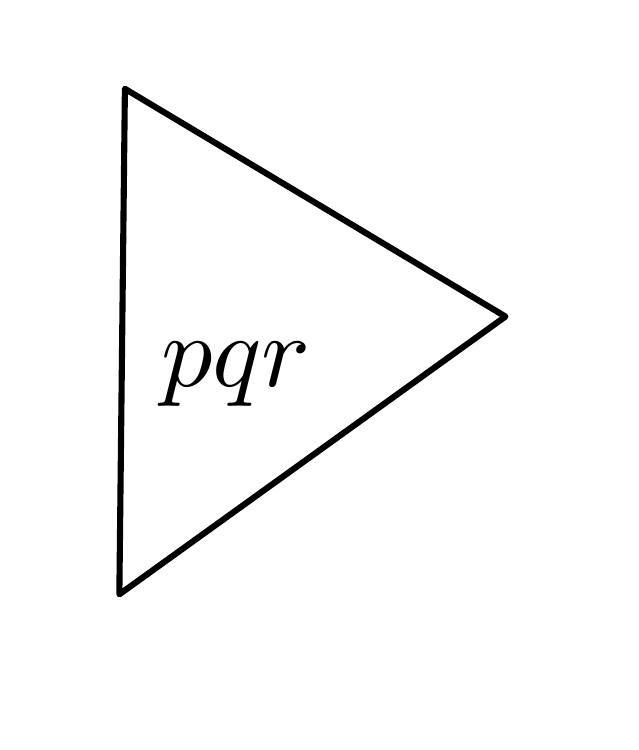
\begin{tikzpicture}[x=1bp,y=-1bp,line cap=round,line join=round]
\path[use as bounding box] (0,0) rectangle (210,250);
\begin{pgfinterruptboundingbox}
\draw[line width=2.2bp] (35,22) -- (172,104) -- (33,204) -- cycle;
\node[inner sep=0pt,outer sep=0pt,anchor=center] at (75,125) {\scalebox{3.7}{\ensuremath{pqr}}};
\end{pgfinterruptboundingbox}
\end{tikzpicture}
}\qquad Gleichung: $px+qy+rz=1$
\end{center}

% A544-P0320-D02
\begin{center}\emph{Coordinaten.}\end{center}
\begin{center}
\begin{minipage}{.28\textwidth}\centering
\resizebox{\linewidth}{!}{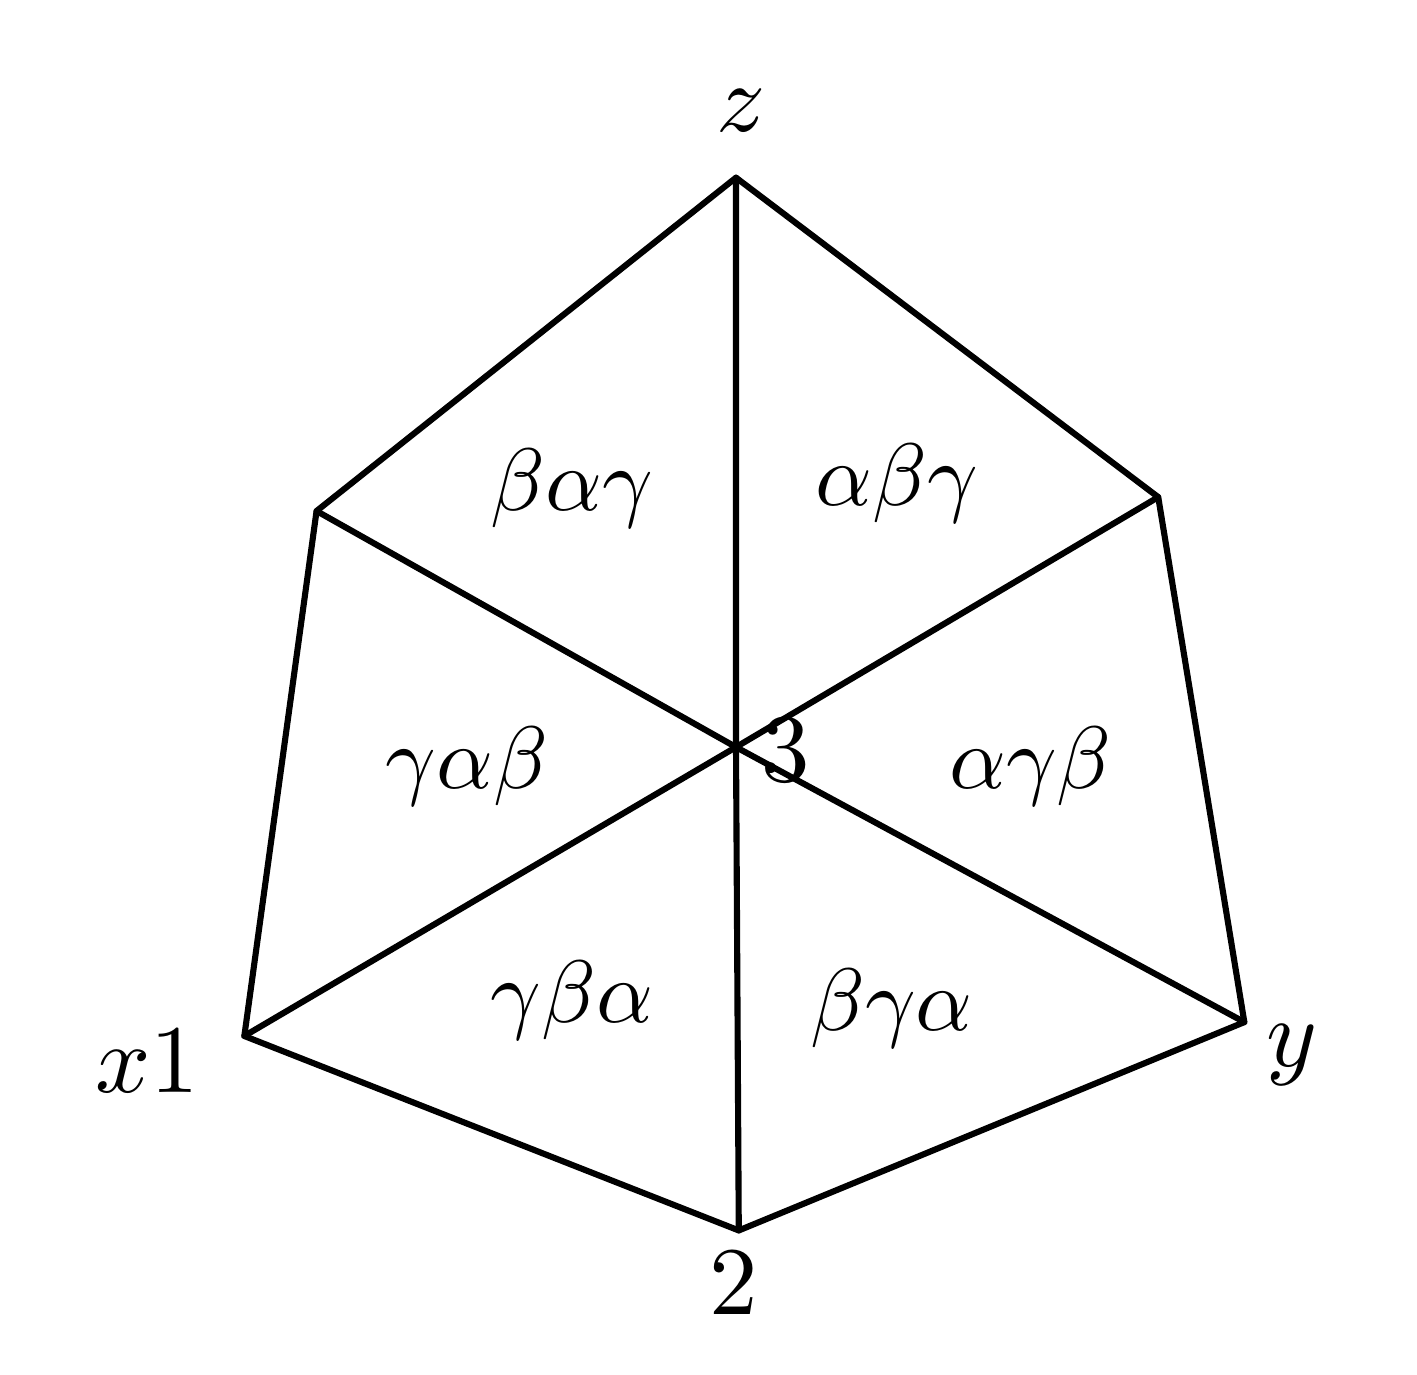
\begin{tikzpicture}[x=1bp,y=-1bp,line cap=round,line join=round]
\path[use as bounding box] (0,0) rectangle (490,475);
\begin{pgfinterruptboundingbox}
\draw[line width=2.2bp] (255,54) -- (407,169) -- (438,358) -- (256,433) -- (78,363) -- (104,174) -- cycle;
\draw[line width=2.2bp] (255,54) -- (255,259) -- (256,433);
\draw[line width=2.2bp] (104,174) -- (255,259) -- (438,358);
\draw[line width=2.2bp] (78,363) -- (255,259) -- (407,169);
\node[inner sep=0pt,outer sep=0pt,anchor=center] at (196,166) {\scalebox{3.2}{\ensuremath{\beta\alpha\gamma}}};
\node[inner sep=0pt,outer sep=0pt,anchor=center] at (313,164) {\scalebox{3.2}{\ensuremath{\alpha\beta\gamma}}};
\node[inner sep=0pt,outer sep=0pt,anchor=center] at (158,266) {\scalebox{3.2}{\ensuremath{\gamma\alpha\beta}}};
\node[inner sep=0pt,outer sep=0pt,anchor=center] at (361,266) {\scalebox{3.2}{\ensuremath{\alpha\gamma\beta}}};
\node[inner sep=0pt,outer sep=0pt,anchor=center] at (196,350) {\scalebox{3.2}{\ensuremath{\gamma\beta\alpha}}};
\node[inner sep=0pt,outer sep=0pt,anchor=center] at (311,353) {\scalebox{3.2}{\ensuremath{\beta\gamma\alpha}}};
\node[inner sep=0pt,outer sep=0pt,anchor=center] at (257,30) {\scalebox{3.5}{\ensuremath{z}}};
\node[inner sep=0pt,outer sep=0pt,anchor=center] at (43,372) {\scalebox{3.5}{\ensuremath{x1}}};
\node[inner sep=0pt,outer sep=0pt,anchor=center] at (455,370) {\scalebox{3.5}{\ensuremath{y}}};
\node[inner sep=0pt,outer sep=0pt,anchor=center] at (254,452) {\scalebox{3.5}{\ensuremath{2}}};
\node[inner sep=0pt,outer sep=0pt,anchor=center] at (273,260) {\scalebox{3.5}{\ensuremath{3}}};
\end{pgfinterruptboundingbox}
\end{tikzpicture}
}
\[\alpha<\beta<\gamma\]
\end{minipage}\hfill
\begin{minipage}{.68\textwidth}
\[
\begin{array}{rccc}
1.&\dfrac1\gamma&0&0\\[1ex]
2.&\dfrac1{\beta+\gamma}&\dfrac1{\beta+\gamma}&0\\[1ex]
3.&\dfrac1{\alpha+\beta+\gamma}&\dfrac1{\alpha+\beta+\gamma}&\dfrac1{\alpha+\beta+\gamma}
\end{array}
\]
\end{minipage}
\end{center}

% A544-P0320-D03
Sechsfacher Inhalt einer Elementarpyramide
\[
=\frac1{\gamma\pdot(\beta+\gamma)(\alpha+\beta+\gamma)}
\]
Alle [Flächen] sind um eine Kugel beschrieben, deren Halbmesser
\[
=\frac1{\surd(\alpha\alpha+\beta\beta+\gamma\gamma)}
\]
Doppelte Fläche eines Dreiecks
\[
=\frac{\surd(\alpha\alpha+\beta\beta+\gamma\gamma)}{\gamma(\beta+\gamma)(\alpha+\beta+\gamma)}
\]
Kante
\[
\begin{aligned}
1\pdot2&=\frac{\surd(\beta\beta+\gamma\gamma)}{\gamma(\beta+\gamma)},\\
1\pdot3&=\frac{\surd((\alpha+\beta)^2+2\gamma\gamma)}{\gamma(\alpha+\beta+\gamma)},\\
2\pdot3&=\frac{\surd(2\alpha\alpha+(\beta+\gamma)^2)}{(\beta+\gamma)(\alpha+\beta+\gamma)}
\end{aligned}
\]
Cosinus Kanten Winkel $3\pdot1\pdot2$
\[
=\frac{\alpha\beta+\beta\beta+\gamma\gamma}{\surd(\beta\beta+\gamma\gamma)((\alpha+\beta)^3+2\gamma\gamma)}
\]
Sinus
\[
=\frac{\gamma\pdot\surd(\alpha\alpha+\beta\beta+\gamma\gamma)}{\surd(\beta\beta+\gamma\gamma)((\alpha+\beta)^2+2\gamma\gamma)}
\]

% A544-P0320-D04
\begin{center}\emph{Vorkommende Werthe.}\end{center}
\begin{center}
\begin{tabular}{rccc l}
&$\alpha$&$\beta$&$\gamma$&\\
7.&0.&0.&1&Hexaeder\\
3.&0.&1.&1&Rhombendodekaeder\\
6.&0.&1.&2&Tetrakishexaeder\\
&0.&1.&3&\\
&0.&2.&3&\\
1.&1.&1.&1&Octaeder\\
5.&1.&1.&2&Trapezicositetraeder\\
&1.&1.&3&\\[1.2ex]
&$\alpha$&$\beta$&$\gamma$&\\
2.&1.&2.&2.&Triakisoctaeder\\
4.&1.&2.&3.&Hexakisoctaeder\\
&1.&2.&4.&\\
2.&1.&3.&3.&Triakisoctaeder\\
4.&1.&3.&5.&Hexakisoctaeder\\
2.&2.&3.&3&Triakisoctaeder\\
&2.&3.&4?&\\
&3.&5.&11&
\end{tabular}
\end{center}
\BookRule{.36\textwidth}


\SourceLeaf{321}%
% A544-P0321-D01
\section*{BEMERKUNGEN.}
\pdfbookmark[1]{Bemerkungen zur geometrischen Seite der ternären Formen}{ternary-bemerkungen}
\BookRule{.15\textwidth}
Neben den vorstehenden Notizen, welche die in der Anzeige von \textsc{Seeber}'s Untersuchungen der ternären Formen gegebenen Gesichtspunkte theilweise weiter entwickeln, sind in der Handschrift mehre eigne mit einem achtzölligen \textsc{Reichenbach}'schen Theodolithen ausgeführte Crystallmessungen aufgezeichnet. Die einzelnen Protokolle enthalten das jedesmalige Datum der Beobachtung, woraus zu ersehen ist, dass diese Untersuchung dem Monat Juli $1831$ angehört.

% A544-P0321-D02
Aus der Theorie der indifferenten ternären quadratischen Formen findet sich im handschriftlichen Nachlass nur der folgende, wahrscheinlich in der Zeit der Ausarbeitung der Disqu. Arr. aufgezeichnete Lehrsatz
\begin{quote}
‘Omnes transformationes formae ternariae
\[
\left(\begin{smallmatrix}1,&1,&-1\\0,&0,&0\end{smallmatrix}\right)
\]
in se ipsam exhibentur per formulam
\[
\begin{array}{ccc}
\alpha\delta+\beta\gamma&\alpha\beta-\gamma\delta&\alpha\beta+\gamma\delta\\[.5ex]
\alpha\gamma-\beta\delta&\frac12(\alpha\alpha+\delta\delta-\beta\beta-\gamma\gamma)&\frac12(\alpha\alpha+\gamma\gamma-\beta\beta-\delta\delta)\\[.5ex]
\alpha\gamma+\beta\delta&\frac12(\alpha\alpha+\beta\beta-\gamma\gamma-\delta\delta)&\frac12(\alpha\alpha+\beta\beta+\gamma\gamma+\delta\delta)
\end{array}
\]
acceptis $\alpha,\beta,\gamma,\delta$ ita ut fiat $\alpha\delta-\beta\gamma=1$.’
\end{quote}

% A544-P0321-D03
Es entstehen nemlich alle Transformationen, in denen die neun Coëfficienten ganze Zahlen sind, wenn für $\alpha,\beta,\gamma,\delta$ sowohl alle die der Bedingungsgleichung genügenden ganzen Zahlen und zwar zwei gerade und zwei ungerade gesetzt werden, als auch alle die ungeraden Vielfache von $\surd\frac12$, welche dieselbe Bedingungsgleichung $\alpha\delta-\beta\gamma=1$ erfüllen.

\SourceLeaf{322}%
% A544-P0322-D01
Zu Seite $309$. Chaux carbonatée équiaxe, inverse, contrastante und mixte sind die von \textsc{Hauy} (Traité de Minéralogie $1801$ Tome II pag. $132$, $137$) gebrauchten Benennungen.

% A544-P0322-D02
Die Tafel der Transformationen der Form $\left(\begin{smallmatrix}5,&5,&5\\1,&1,&1\end{smallmatrix}\right)$ enthält in der ersten Verticalreihe die Coëfficienten der Substitution, in der zweiten die dadurch entstandene neue Form, in der dritten die der letztern Form entsprechende primitive, wenn diese nicht selbst schon eine solche ist, und in der vierten deren Adjuncta.
\begin{flushright}\textsc{Schering.}\end{flushright}
\BookRule{.30\textwidth}

\SourceLeaf{323}%
% A544-P0323-D01
\chapter*{ZUR THEORIE DER BIQUADRATISCHEN RESTE.}
\pdfbookmark[0]{Zur Theorie der biquadratischen Reste}{nachlass-biquadratic}
\renewcommand{\BookRunningTitle}{Zur Theorie der biquadratischen Reste}
\BookRule{.18\textwidth}
\begin{center}\textbf{[I.]}\end{center}
\pdfbookmark[1]{I}{nachlass-biquadratic-I}
\renewcommand{\Article}[1]{\par\medskip\Needspace{4\baselineskip}\pdfbookmark[2]{Art. #1}{nachlass-biquadratic-I-art-#1}\centerline{\textbf{#1.}}\nobreak\smallskip}
\Article{1}
Wir erweitern das Gebiet der höhern Arithmetik, indem wir darin auch die imaginären Grössen aufnehmen. Bei der gegenwärtigen Untersuchung nennen wir eine ganze imaginäre Zahl jede Grösse $x+iy$, wenn $x,y$ reelle ganze Zahlen sind.

% A544-P0323-D02
\Article{2}
Die unendliche Anzahl imaginärer ganzer Zahlen lässt sich am bequemsten durch Punkte in einer unbegrenzten Ebene sinnlich darstellen; wir nennen schlechthin denjenigen Punkt, dessen Abscisse $x$, die Ordinate $y$ ist, den Punkt $x+iy$, alle Punkte, die ganze Zahlen vorstellen, sollen Ganzepunkte heissen.

% A544-P0323-D03
\Article{3}
Um etwas bestimmtes festzusetzen, sollen die Abscissen immer auf der linken Seite positiv, die Ordinaten oben positiv sein.

% A544-P0323-D04
\Article{4}
Die gerade Linie von dem Punkte $x+iy$ zu dem Punkte $x'+iy'$ gezogen soll schlechtweg die gerade Linie $(x+iy,x'+iy')$ heissen, wir nehmen dabei zugleich, insofern es darauf ankommt, auf die Richtung Rücksicht und unterscheiden also die gerade Linie $x+iy,x'+iy'$ von der $x'+iy',x+iy$.

\SourceLeaf{324}%
% A544-P0324-D01
\Article{5}
Der Kürze wegen wollen wir imaginäre Grössen wie $x+iy$ auch durch einen einzigen Buchstaben bezeichnen, wie $z$.

% A544-P0324-D02
\Article{6}
Die Figur, welche durch die geraden Linien $zz',z'z'',z''z'''\ldots z^{n-1}z^n,z^nz$ begrenzt wird, nennen wir schlechtweg die Figur $zz'z''z'''\dotstwo z^n$. Wir schliessen dabei den Fall nicht aus, wo etwa einige dieser Linien einander schneiden.

% A544-P0324-D03
\Article{7}
Durch $S(z,z',z''\ldots z^n)$ bezeichnen wir allgemein die Summe von so vielen reellen ganzen Zahlen, als Ganzepunkte innerhalb der Figur liegen, indem wir für jeden Punkt, um den die Grenzlinie der Figur einmal, zweimal, dreimal u.s.w. herumgeht, die Zahl $\pm1$, $\pm2$, $\pm3$ etc. setzen; die obern Zeichen gelten, wenn die Grenzlinie den Punkt so umgibt, dass dieser auf der rechten Seite der Figur liegt, die untern im entgegengesetzten Fall. Schneiden sich also keine Seiten der Figur, so ist $S(z,z',z''\dotstwo)$ schlechthin die Anzahl der Punkte innerhalb der Figur, positiv oder negativ genommen.

% A544-P0324-D04
\Article{8}
Offenbar ist immer
\[
\begin{aligned}
S(z,z',z''\ldots z^n)&=S(z',z'',z'''\dotstwo z^n,z)\\
&=S(z'',z'''\dotstwo z')\text{ etc.}\\
&=-S(z^n,z^{n-1}\dotstwo z'',z',z)\\
&=-S(z^{n-1}\pdot z^{n-2}\dotstwo z',z,z^n)\text{ etc.}
\end{aligned}
\]

% A544-P0324-D05
\Article{9}
Wie es hiebei mit den auf der Grenzlinie selbst liegenden Punkten gehalten werden soll, muss noch näher bestimmt werden. Es gibt viele Fälle, wo auf der Grenzlinie gar keine ganze Punkte liegen können: dann ist keine Bestimmung nöthig. Liegen aber auf der Grenzlinie $zz'$ solche Punkte, so zeigen wir durch ein zwischen $z$ und $z'$ eingeschobenes $+$ an, dass diese Punkte so betrachtet werden sollen, als lägen sie rechts von der Grenzlinie, so wie durch ein $-$, als lägen sie links. Auch werden wir wol ein $0$ oder $\frac12$ einschieben, wodurch angedeutet werden soll, dass sie gar nicht oder nur mit dem halben Werthe auf
\SourceLeaf{325}%
% A544-P0325-D01
jeder Seite in Betracht gezogen werden sollen. Falls einer oder der andere der Punkte $z,z',z''$ etc. selbst ein Ganzepunkt, so wird er, wo nicht ausdrücklich das Gegentheil gesagt wird, gar nicht mitgezählt, als insofern er zugleich etwa als Nicht-Eckpunkt auch in Betracht kommt.

% A544-P0325-D02
\Article{10}
Lehrsätze. Wenn alle $z,z',z''$ etc. um eine und dieselbe Ganzezahl vermehrt werden, so bleibt das $S$ ungeändert.

% A544-P0325-D03
Wenn $i$ in $-i$ und jedes Bindezeichen ins entgegengesetzte verwandelt wird, so ändert $S$ bloss das Zeichen.
\[
\begin{aligned}
S(z,z',z''\ldots z^n)={}&S(z,u,u'\dotstwo u^n,z',z'',z^n)\\
&-S(z,u,u'\dotstwo u^n,z')\\
={}&S(z,u,u',u''\dotstwo u^n,z^m,z^{m+1}\dotstwo z^n)\\
&-S(z,u,u',u''\dotstwo u^n,z^m,z^{m-1}\dotstwo z',z)
\end{aligned}
\]
wo die Bindezeichen correspondiren müssen, aber zwischen den rückwärts laufenden Gliedern entgegengesetzt werden.

% A544-P0325-D04
Ist $\zeta$ eine ganze Zahl $=a+bi$, so ist, wenn die gegenüberliegenden Bindezeichen entgegengesetzt,
\[
S(z,z',z'+\zeta,z+\zeta)=[bx'-ay']-[bx-ay]
\]
Hiebei ist zu bemerken, dass wenn $bx'-ay'$ selbst eine ganze Zahl ist, diese für $[bx'-ay']$ angenommen werde, wenn das Bindezeichen zwischen $z'$ und $z'+\zeta$ $+$ ist, hingegen $1$ oder $\frac12$ weniger, wenn dieses Bindezeichen $-$ oder $\frac12$ ist; bei $bx-ay$ gilt das Umgekehrte.

% A544-P0325-D05
Uebrigens gilt die Formel nur für den Fall, wo $a$ und $b$ keinen gemeinschaftlichen Divisor haben; ist ihr grösster gemeinschaftlicher Theiler $=h$, so hat man dafür zu nehmen
\[
h\left[\frac{bx'-ay'}h\right]-h\left[\frac{bx-ay}h\right]
\]

% A544-P0325-D06
\Article{11}
Wenden wir uns nun näher zu unserm Gegenstande selbst. Wenn für den Modulus $m=a+bi$ die Zahlen $f,f',f''$ etc. so beschaffen sind, dass sie erstlich alle nach dem Modulus $m$ unter sich incongruent sind, zweitens aber jede ganze Zahl einer von ihnen nothwendig congruent sein muss, so nennen wir den

\SourceLeaf{326}%
% A544-P0326-D01
Inbegriff der Zahlen $f,f',f''$ etc. das System der Primitivreste von $m$. Ihre Anzahl ist immer $=aa+bb$.

% A544-P0326-D02
\Article{12}
Man kann das System der Primitivreste auf vielfache Art bilden; die einfachste ist, die Punkte innerhalb des Quadrats $0,m,(1+i)m,im$ zu wählen; dazu müssen aber noch hinzugefügt werden
\begin{enumerate}
\item[I.] der Punkt oder die Grösse $0$
\item[II.] alle Punkte auf zwei einander nicht gegenüberliegenden Grenzlinien.
\end{enumerate}
Anstatt auf einer der $4$ Grenzlinien alle Punkte zu nehmen, kann man sie auch auf mehren zugleich nehmen.

% A544-P0326-D03
Diese Auswahl dieser Punkte auf den Grenzlinien, falls welche darauf fallen, kann auf mehrfache Art geschehen, so dass obigen Bedingungen Genüge geschieht. Am einfachsten ist die folgende Manier.

% A544-P0326-D04
Man nehme auf der Grenzlinie $0,m$ alle Punkte zwischen $0$ und $\frac12m$ inclus. und auf der Grenzlinie $0,im$ alle Punkte von $\frac12im$ bis $im$ exclusive und auf ähnliche Art bei den beiden andern.

% A544-P0326-D05
Man kann diese beiden Manieren so sinnlich darstellen
\begin{center}\resizebox{.85\textwidth}{!}{\begin{tikzpicture}[x=1bp,y=-1bp,line cap=round,line join=round]
\path[use as bounding box] (0,0) rectangle (1230,440);
\begin{pgfinterruptboundingbox}
\draw[line width=2.2bp] (228,69) -- (72,214) -- (218,366) -- (373,219) -- (326,168);
\draw[line width=2.2bp] (322,163) -- (257,96);
\draw[line width=2.2bp] (250,90) -- (228,69);
\draw[line width=2bp] (148,136) circle[radius=5bp];
\draw[line width=2bp] (304,140) circle[radius=5bp];
\draw[line width=2bp] (297,284) circle[radius=5bp];
\draw[line width=2bp] (152,290) circle[radius=5bp];
\node[inner sep=0pt,outer sep=0pt,anchor=center] at (53,214) {\scalebox{3.5}{\ensuremath{m}}};
\node[inner sep=0pt,outer sep=0pt,anchor=center] at (228,48) {\scalebox{3.5}{\ensuremath{(1+i)m}}};
\node[inner sep=0pt,outer sep=0pt,anchor=center] at (399,220) {\scalebox{3.5}{\ensuremath{im}}};
\node[inner sep=0pt,outer sep=0pt,anchor=center] at (213,387) {\scalebox{3.5}{\ensuremath{0}}};
\draw[line width=2.2bp] (839,229) -- (993,77) -- (1143,234) -- (987,378) -- cycle;
\draw[line width=2bp] (878,197) circle[radius=5bp];
\draw[line width=2bp] (906,155) circle[radius=5bp];
\draw[line width=2bp] (951,112) circle[radius=5bp];
\draw[line width=2bp] (1023,116) circle[radius=5bp];
\draw[line width=2bp] (1069,151) circle[radius=5bp];
\draw[line width=2bp] (1112,193) circle[radius=5bp];
\draw[line width=2bp] (869,270) circle[radius=5bp];
\draw[line width=2bp] (915,303) circle[radius=5bp];
\draw[line width=2bp] (956,344) circle[radius=5bp];
\draw[line width=2bp] (984,373) circle[radius=5bp];
\draw[line width=2bp] (1024,352) circle[radius=5bp];
\draw[line width=2bp] (1055,309) circle[radius=5bp];
\draw[line width=2bp] (1098,269) circle[radius=5bp];
\node[inner sep=0pt,outer sep=0pt,anchor=center] at (819,229) {\scalebox{3.5}{\ensuremath{m}}};
\node[inner sep=0pt,outer sep=0pt,anchor=center] at (991,54) {\scalebox{3.5}{\ensuremath{(1+i)m}}};
\node[inner sep=0pt,outer sep=0pt,anchor=center] at (1166,236) {\scalebox{3.5}{\ensuremath{im}}};
\node[inner sep=0pt,outer sep=0pt,anchor=center] at (978,397) {\scalebox{3.5}{\ensuremath{0}}};
\end{pgfinterruptboundingbox}
\end{tikzpicture}
}\end{center}

% A544-P0326-D06
\Article{13}
Schliesst man von den Primitivpunkten aus
\begin{enumerate}
\item[I.] Bloss den Punkt $0$, wenn $a$ gerade und $b$ ungerade oder umgekehrt.
\item[II.] Die Punkte $0$ und $\frac12(1+i)m$, wenn $a$ und $b$ beide ungerade.
\item[III.] Die vier Punkte $0,\frac12m,\frac12(1+i)m,\frac12im$, wenn $a$ und $b$ beide gerade,
\end{enumerate}
so nennen wir die übrigbleibenden eigentliche Primitivpunkte, die ausgeschlossenen uneigentliche. Die Anzahl von jenen ist also
\[
\begin{array}{rrcl}
\text{in Fall}&\mathrm{I}&=&aa+bb-1\\
&\mathrm{II}&=&aa+bb-2\\
&\mathrm{III}&=&aa+bb-4
\end{array}
\]
also immer durch $4$ theilbar.

\SourceLeaf{327}%
% A544-P0327-D01
\Article{14}
Diese eigentlichen Primitivpunkte lassen sich in $4$ Classen $F,F',F'',F'''$ theilen, so dass
\[
\begin{array}{llll}
iF\equiv F'&iF'\equiv F''&iF''\equiv F'''&iF'''\equiv F\\
-F\equiv F''&-F'\equiv F'''&-F''\equiv F&-F'''\equiv F'\\
-iF\equiv F'''&-iF'\equiv F&-iF''\equiv F'&-iF'''\equiv F''
\end{array}
\]
Hiebei findet nun folgendes höchst wichtige Theorem statt.

% A544-P0327-D02
Es sei $M$ eine Zahl, welche mit $m$ keinen Factor gemein hat. Von den Zahlen $MF$ gehören in die Classe $F$ eine Anzahl von $n$
\[
\begin{array}{cc}F'&n'\\F''&n''\\F'''&n'''\end{array}
\]
und der kleinste Rest von $n'+2n''+3n''$ nach dem Modulus $4$ sei $=N$, also $N$ einer der $4$ Zahlen $0,1,2,3$ gleich: unter dieser Voraussetzung ist $N$ \emph{unabhängig} von der Art der Vertheilung der Primitivreste in Classen. Wir nennen ihn den Decident des biquadratischen Verhältnisses der Zahl $M$ zu $m$.

% A544-P0327-D03
\Article{15}
Die einfachste Art der Vertheilung ist allerdings folgende
\begin{center}\resizebox{.35\textwidth}{!}{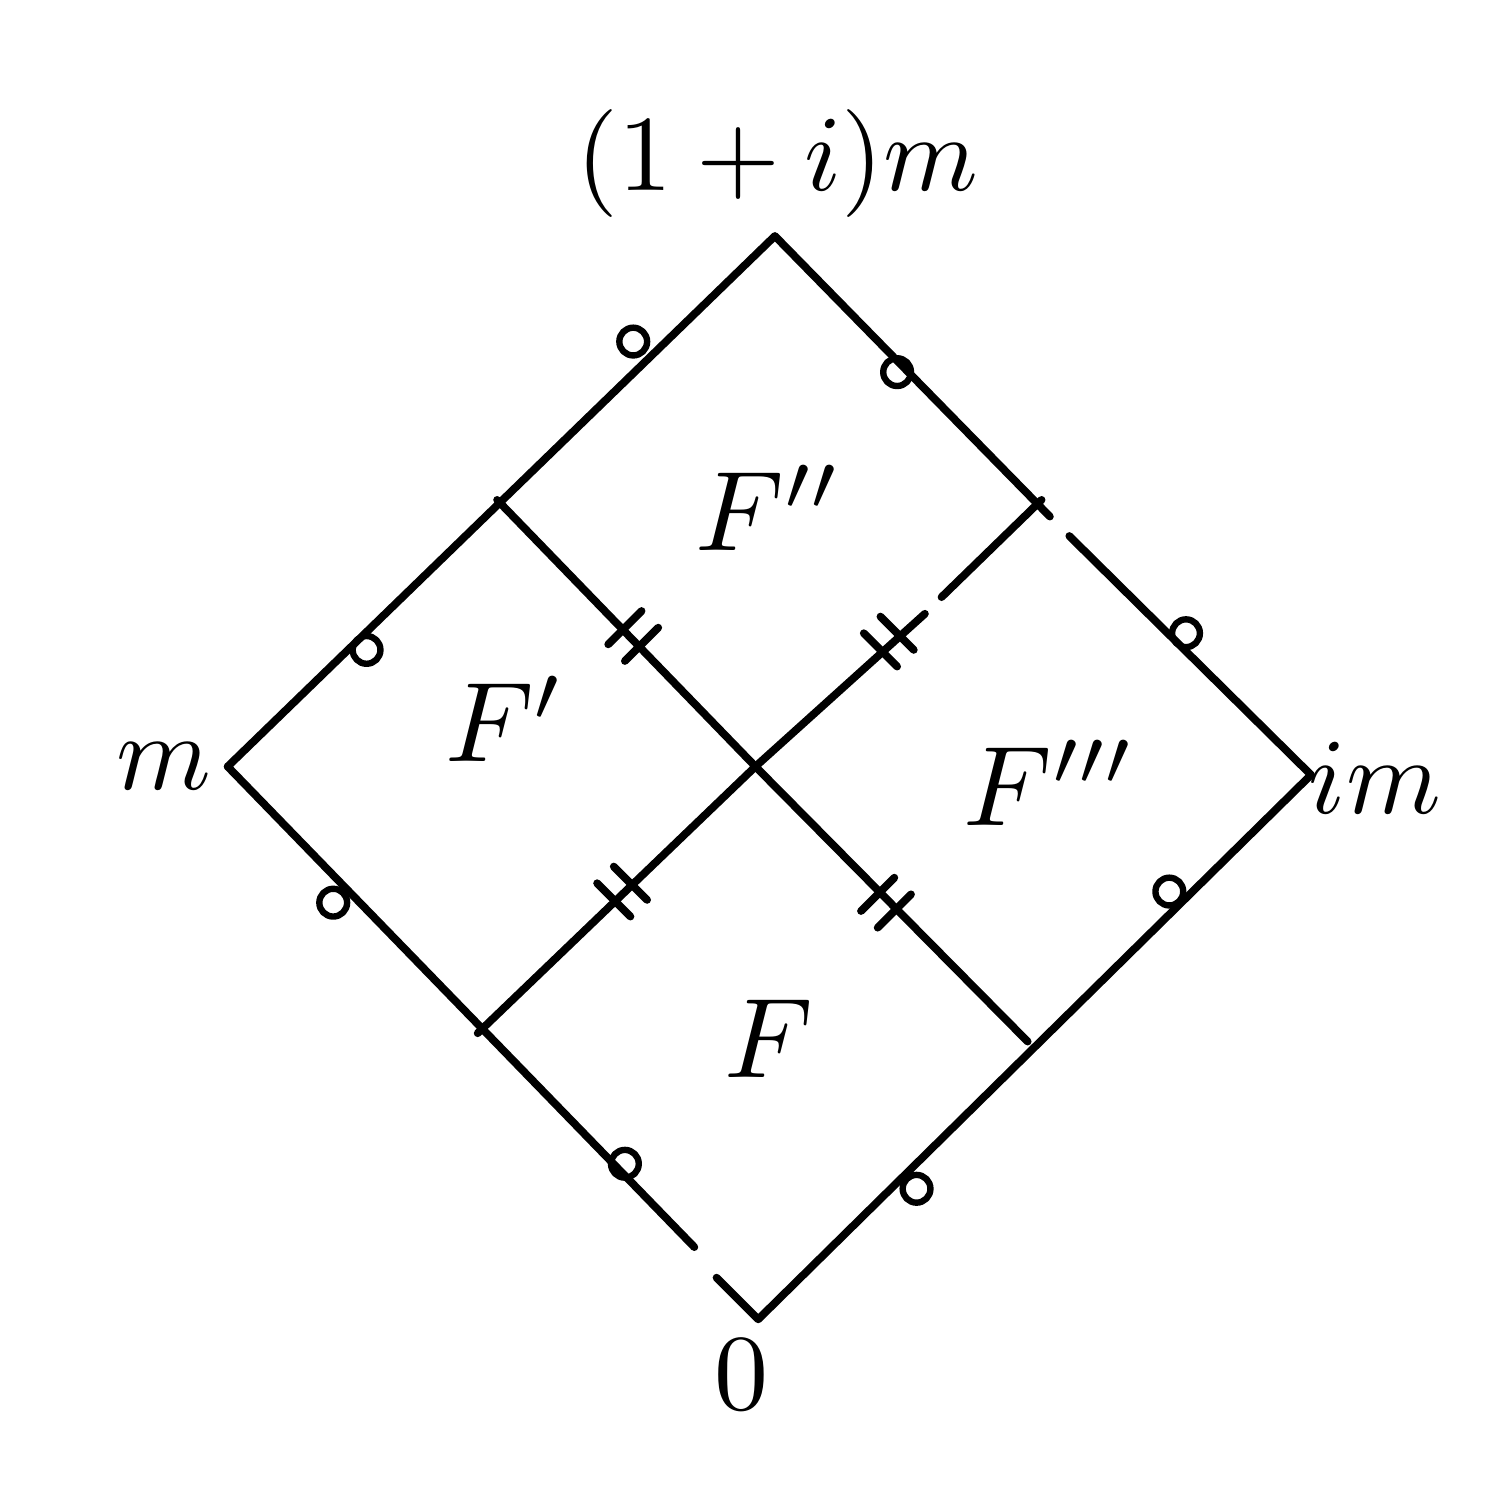
\begin{tikzpicture}[x=1bp,y=-1bp,line cap=round,line join=round]
\path[use as bounding box] (0,0) rectangle (520,520);
\begin{pgfinterruptboundingbox}
\draw[line width=2.8bp] (72,266) -- (269,75) -- (368,176);
\draw[line width=2.8bp] (375,183) -- (462,269) -- (263,465) -- (248,450);
\draw[line width=2.8bp] (240,439) -- (72,266);
\draw[line width=2.8bp] (169,170) -- (262,266) -- (360,365);
\draw[line width=2.8bp] (365,170) -- (329,205);
\draw[line width=2.8bp] (323,211) -- (262,266) -- (162,362);
\draw[line width=2.3bp] (218,113) circle[radius=5bp];
\draw[line width=2.3bp] (313,124) circle[radius=5bp];
\draw[line width=2.3bp] (122,224) circle[radius=5bp];
\draw[line width=2.3bp] (417,218) circle[radius=5bp];
\draw[line width=2.3bp] (110,315) circle[radius=5bp];
\draw[line width=2.3bp] (411,311) circle[radius=5bp];
\draw[line width=2.3bp] (215,409) circle[radius=5bp];
\draw[line width=2.3bp] (320,418) circle[radius=5bp];
\draw[line width=2.8bp] (209,222) -- (221,210);
\draw[line width=2.8bp] (215,228) -- (227,216);
\draw[line width=2.8bp] (301,218) -- (313,230);
\draw[line width=2.8bp] (307,212) -- (319,224);
\draw[line width=2.8bp] (205,308) -- (217,320);
\draw[line width=2.8bp] (211,302) -- (223,314);
\draw[line width=2.8bp] (300,318) -- (312,306);
\draw[line width=2.8bp] (306,324) -- (318,312);
\node[inner sep=0pt,outer sep=0pt,anchor=center] at (267,173) {\scalebox{4.1}{\ensuremath{F''}}};
\node[inner sep=0pt,outer sep=0pt,anchor=center] at (172,249) {\scalebox{4.1}{\ensuremath{F'}}};
\node[inner sep=0pt,outer sep=0pt,anchor=center] at (368,272) {\scalebox{4.1}{\ensuremath{F'''}}};
\node[inner sep=0pt,outer sep=0pt,anchor=center] at (267,364) {\scalebox{4.1}{\ensuremath{F}}};
\node[inner sep=0pt,outer sep=0pt,anchor=center] at (49,266) {\scalebox{3.9}{\ensuremath{m}}};
\node[inner sep=0pt,outer sep=0pt,anchor=center] at (270,49) {\scalebox{3.9}{\ensuremath{(1+i)m}}};
\node[inner sep=0pt,outer sep=0pt,anchor=center] at (485,270) {\scalebox{3.9}{\ensuremath{im}}};
\node[inner sep=0pt,outer sep=0pt,anchor=center] at (257,485) {\scalebox{3.9}{\ensuremath{0}}};
\end{pgfinterruptboundingbox}
\end{tikzpicture}
}\end{center}
Inzwischen kann in speciellen Fällen eine andere Vertheilung vortheilhafter sein.

% A544-P0327-D04
\Article{16}
Sind $f,f',f''$ etc. die sämmtlichen Primitivreste des Modulus $m$, so ist
\SourceLeaf{328}%
% A544-P0328-D01
\[
\begin{aligned}
&S(z+\tfrac fm,\ z'+\tfrac fm,\ z''+\tfrac fm,\ \text{etc.})\\
&+S(z+\tfrac{f'}m,\ z'+\tfrac{f'}m,\ z''+\tfrac{f'}m,\ \text{etc.})\\
&+S(z+\tfrac{f''}m,\ z'+\tfrac{f''}m,\ z''+\tfrac{f''}m,\ \text{etc.})\\
&+\text{etc.}\\
&=S(mz,mz',mz'',\ \text{etc.}
\end{aligned}
\]

% A544-P0328-D02
\Article{17}
\begin{center}\emph{Theorie des biquadratischen Restes} $1+i$.\end{center}
Der Modulus soll mit dem Reste keinen Theiler gemein haben, wir nehmen also an, dass von den Zahlen $a$ und $b$ die eine gerade, die andere ungerade sei. Die Vertheilung der eigentlichen Primitivreste in die vier Classen stellt folgendes Schema vor
\begin{center}\resizebox{.90\textwidth}{!}{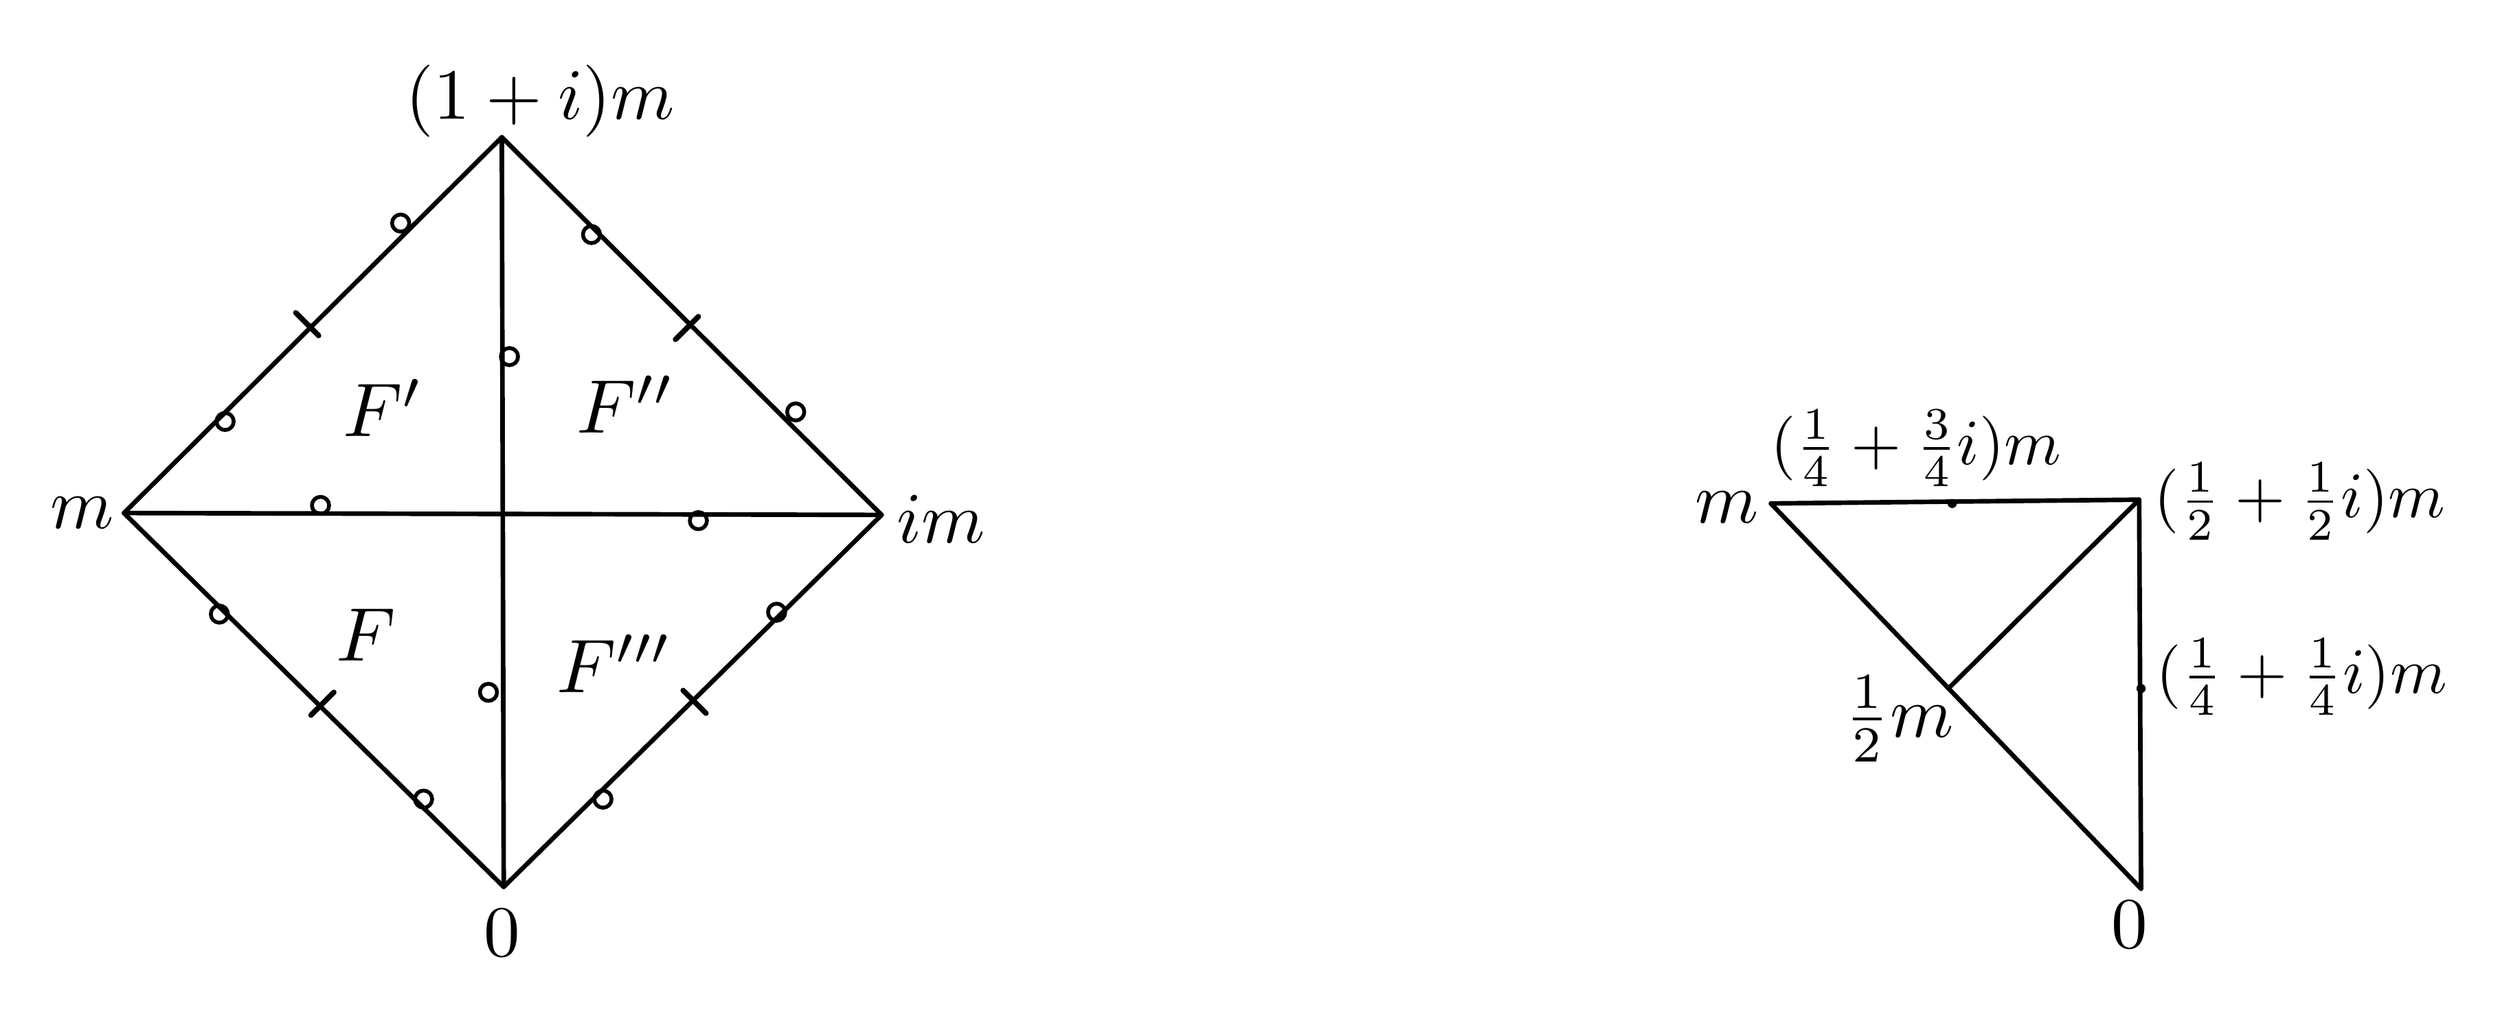
\begin{tikzpicture}[x=1bp,y=-1bp,line cap=round,line join=round]
\path[use as bounding box] (0,0) rectangle (1290,520);
\begin{pgfinterruptboundingbox}
\draw[line width=2.4bp] (55,259) -- (253,62) -- (452,260) -- (254,455) -- cycle;
\draw[line width=2.4bp] (253,62) -- (254,455);
\draw[line width=2.4bp] (55,259) -- (452,260);
\draw[line width=2bp] (108,211) circle[radius=4.5bp];
\draw[line width=2bp] (200,107) circle[radius=4.5bp];
\draw[line width=2bp] (300,113) circle[radius=4.5bp];
\draw[line width=2bp] (407,206) circle[radius=4.5bp];
\draw[line width=2bp] (105,312) circle[radius=4.5bp];
\draw[line width=2bp] (212,409) circle[radius=4.5bp];
\draw[line width=2bp] (397,311) circle[radius=4.5bp];
\draw[line width=2bp] (306,409) circle[radius=4.5bp];
\draw[line width=2bp] (158,255) circle[radius=4.5bp];
\draw[line width=2bp] (356,263) circle[radius=4.5bp];
\draw[line width=2bp] (257,177) circle[radius=4.5bp];
\draw[line width=2bp] (246,353) circle[radius=4.5bp];
\draw[line width=2.8bp] (145,154) -- (157,166);
\draw[line width=2.8bp] (344,168) -- (356,156);
\draw[line width=2.8bp] (153,365) -- (165,353);
\draw[line width=2.8bp] (348,352) -- (360,364);
\node[inner sep=0pt,outer sep=0pt,anchor=center] at (191,204) {\scalebox{4}{\ensuremath{F'}}};
\node[inner sep=0pt,outer sep=0pt,anchor=center] at (318,202) {\scalebox{4}{\ensuremath{F''}}};
\node[inner sep=0pt,outer sep=0pt,anchor=center] at (182,323) {\scalebox{4}{\ensuremath{F}}};
\node[inner sep=0pt,outer sep=0pt,anchor=center] at (312,338) {\scalebox{4}{\ensuremath{F'''}}};
\node[inner sep=0pt,outer sep=0pt,anchor=center] at (33,259) {\scalebox{3.8}{\ensuremath{m}}};
\node[inner sep=0pt,outer sep=0pt,anchor=center] at (273,43) {\scalebox{3.8}{\ensuremath{(1+i)m}}};
\node[inner sep=0pt,outer sep=0pt,anchor=center] at (483,262) {\scalebox{3.8}{\ensuremath{im}}};
\node[inner sep=0pt,outer sep=0pt,anchor=center] at (253,479) {\scalebox{3.8}{\ensuremath{0}}};
\draw[line width=2.4bp] (918,254) -- (1111,252) -- (1112,456) -- cycle;
\draw[line width=2.4bp] (1011,351) -- (1111,252);
\fill (1013,254) circle[radius=2.4bp];
\fill (1112,351) circle[radius=2.4bp];
\node[inner sep=0pt,outer sep=0pt,anchor=center] at (895,256) {\scalebox{3.8}{\ensuremath{m}}};
\node[inner sep=0pt,outer sep=0pt,anchor=center] at (994,225) {\scalebox{3.4}{\ensuremath{(\frac14+\frac34 i)m}}};
\node[inner sep=0pt,outer sep=0pt,anchor=west] at (1119,253) {\scalebox{3.4}{\ensuremath{(\frac12+\frac12 i)m}}};
\node[inner sep=0pt,outer sep=0pt,anchor=center] at (985,367) {\scalebox{3.8}{\ensuremath{\frac12 m}}};
\node[inner sep=0pt,outer sep=0pt,anchor=west] at (1120,345) {\scalebox{3.4}{\ensuremath{(\frac14+\frac14 i)m}}};
\node[inner sep=0pt,outer sep=0pt,anchor=center] at (1106,475) {\scalebox{3.8}{\ensuremath{0}}};
\end{pgfinterruptboundingbox}
\end{tikzpicture}
}\end{center}

% A544-P0328-D03
Zu $n$ sind zu rechnen alle Zahlen auf
\[
\text{der Linie }0\ldots\tfrac12m\qquad\text{Anzahl }=g
\]
Zu $n'$ alle Zahlen auf
\[
\text{der Linie }0\ldots(\tfrac14+\tfrac14i)m\qquad\text{Anzahl }=g'
\]
Zu $n''$ alle Zahlen innerhalb
\[
\text{des Dreiecks }\tfrac12m,m,(\tfrac12+\tfrac12i)m\qquad\text{Anzahl }=h
\]
Zu $n'''$ alle Zahlen innerhalb
\[
\text{des Dreiecks }0,\tfrac12m,(\tfrac12+\tfrac12i)m\qquad\text{Anzahl }=h'
\]
und ausserdem alle Zahlen auf
\[
\text{der Linie }(\tfrac14+\tfrac14i)m\dotstwo(\tfrac12+\tfrac12i)m\qquad\text{Anzahl }=g''
\]

% A544-P0328-D04
Man hat immer $g'+g''=g$, $aa+bb=p$, $\frac14(p-1)=g+g'+g''+h+h'$ Der Decident ist also
\SourceLeaf{329}%
% A544-P0329-D01
\[
D=S(0_{(+)},\tfrac12m,(\tfrac12+\tfrac12i)m_{(-)})+\tfrac12(p-1)+2g''
\]

% A544-P0329-D02
Man nehme nun an, dass für den Modulus $m+1+i$
\[
\begin{array}{clc}
g&\text{übergehe in}&G\\
g'&&G'\\
g''&&G''\\
h&&H\\
h'&&H'
\end{array}
\]
so hat man
\[
\begin{aligned}
&\Delta S(0_{(+)},\tfrac12m,(\tfrac12+\tfrac12i)m_{(-)})\\
&\quad=+S(0_{(+)},(\tfrac12+\tfrac12i)m,(\tfrac12+\tfrac12i)m+i_{(-)})\\
&\qquad-S(0_{(+)},\tfrac12m,\tfrac12m+\tfrac12+\tfrac12i_{(-)})\\
&\qquad-S(\tfrac12m,(\tfrac12+\tfrac12i)m,(\tfrac12+\tfrac12i)m+i,\ \tfrac12m+\tfrac12+\tfrac12i)
\end{aligned}
\]

% A544-P0329-D03
Das letzte dieser $S$ ist
\[
=\left[\tfrac12(a-b)\right]-\left[\tfrac12a\right]-S((\tfrac12+\tfrac12i)m,\tfrac12m,\tfrac12m+\tfrac12-\tfrac12i)
\]
wenn $a$ ungerade oder gerade
\[
\begin{aligned}
={}&\left[\tfrac12(a-b)\right]-\left[\tfrac12a\right]-S(-\tfrac12+\tfrac12i,\tfrac12m-\tfrac12+\tfrac12i,\tfrac12m+i)\\
={}&\left[\tfrac12(a-b)\right]-\left[\tfrac12a\right]+S(0_{(+)},\tfrac12m,\tfrac12m+\tfrac12+\tfrac12i_{(-)})\\
&-S(0_{(+)},(\tfrac12+\tfrac12i)m,(\tfrac12+\tfrac12i)m+i_{(-)})
\end{aligned}
\]

% A544-P0329-D04
Also
\[
\begin{aligned}
\Delta D={}&-\left[\tfrac12(a-b)\right]+\left[\tfrac12a\right]\\
&+2S(0_{(+)},(\tfrac12+\tfrac12i)m,(\tfrac12+\tfrac12i)m+i_{(-)})+a+b+1\\
&-2S(0_{(+)},\tfrac12m,\tfrac12m+\tfrac12+\tfrac12i_{(-)})-2g''+2G''
\end{aligned}
\]

% A544-P0329-D05
Die Bindezeichen gelten alle für den Fall, wo $a-b$ positiv ist, sonst nimmt man die entgegengesetzten.

% A544-P0329-D06
Wir zerlegen ferner $S(0_{(+)},(\frac12+\frac12i)m,(\frac12+\frac12i)m+i_{(-)})$ in
\[
\begin{aligned}
&S(0_{(+)},(\tfrac14+\tfrac14i)m,(\tfrac14+\tfrac14m)+\tfrac12i_{(-)})\\
&+\left[\tfrac12(a-b)\right]-\left[\tfrac14(a-b)\right]\\
&-S((\tfrac12+\tfrac12i)m_{(-)},(\tfrac14+\tfrac14i)m,(\tfrac14+\tfrac14i)m-\tfrac12i_{(-)})
\end{aligned}
\]

\SourceLeaf{330}%
% A544-P0330-D01
Der letzte Theil
\[
\begin{aligned}
={}&-S(\tfrac12+\tfrac12i_{(-)},(-\tfrac14-\tfrac14i)m+\tfrac12+\tfrac12i,\ (-\tfrac14-\tfrac14i)m+\tfrac12_{(+)})\\
={}&-S(-\tfrac12-\tfrac12i_{(-)},(\tfrac14+\tfrac14i)m-\tfrac12-\tfrac12i,\ (\tfrac14+\tfrac14i)m-\tfrac12_{(+)})\\
={}&-S(-\tfrac12-\tfrac12i_{(+)},(\tfrac14+\tfrac14i)m-\tfrac12-\tfrac12i,\ (\tfrac14+\tfrac14i)m-\tfrac12_{(-)})+g''-G''\\
={}&S(0_{(+)},(\tfrac14+\tfrac14i)m,(\tfrac14+\tfrac14i)m+\tfrac12i_{(-)})\\
&-S(0_{(+)},\tfrac12m,\tfrac12m+\tfrac12+\tfrac12i_{(-)})+g''-G''
\end{aligned}
\]

% A544-P0330-D02
Dadurch wird also
\[
\begin{aligned}
\Delta D={}&+\left[\tfrac12(a-b)\right]+\left[\tfrac12a\right]\\
&-4S(-\tfrac12-\tfrac12i_{(+)},\tfrac14+\tfrac14im-\tfrac12-\tfrac12i,\ (\tfrac14+\tfrac14i)m-\tfrac12_{(-)})\\
&-2\left[\tfrac14(a-b)\right]+a+b+1
\end{aligned}
\]

% A544-P0330-D03
Für den Fall der Vermehrung des Modulus um $1-i,-1+i,-1-i$ ist keine besondere Untersuchung nöthig, weil offenbar die Moduli $m,im,-m,-im$ gleiche Decidenten haben. Wir haben also folgende Lehrsätze:

% A544-P0330-D04
Ist der Decident des Modulus $a+bi,=D$, so sind die Decidenten von
{\small
\[
\begin{array}{l|l}
a+1+(b+1)i&D+a+b+1+[\tfrac12a]+[\tfrac12(a-b)]-2[\tfrac14(a-b)]\\
a+1+(b-1)i&D+a-b+1+[-\tfrac12b]+[-\tfrac12(a+b)]-2[-\tfrac14(a+b)]\\
a-1+(b+1)i&D-a+b+1+[\tfrac12b]+[\tfrac12(a+b)]-2[\tfrac14(a+b)]\\
a-1+(b-1)i&D-a-b+1+[-\tfrac12a]+[\tfrac12(b-a)]-2[\tfrac14(b-a)]
\end{array}
\]
}

% A544-P0330-D05
Hieraus ferner
{\footnotesize
\[
\begin{array}{l|l|l}
&&\begin{gathered}\text{oder insofern }a\text{ un-}\\\text{gerade ist}\end{gathered}\\
a+2+bi&\begin{aligned}D-\tfrac{a-b-3}2+2[\tfrac12a]&-2[\tfrac{a-b}4]\\&-2[\tfrac{-a-b-2}4]\end{aligned}&D+\tfrac{b-a-1}2\\[1ex]
a-2+bi&\begin{aligned}D+\tfrac{a-b+3}2+2[-\tfrac12a]&-2[\tfrac{b-a}4]\\&-2[\tfrac{a+b-2}4]\end{aligned}&D\\[1ex]
a+(b+2)i&\begin{aligned}D-\tfrac{a+b-3}2+2[\tfrac12b]&-2[\tfrac{a+b}4]\\&-2[\tfrac{a-b-2}4]\end{aligned}&D+\tfrac{a+b-3}2\\[1ex]
a+(b-2)i&\begin{aligned}D+\tfrac{a+b+3}2+2[-\tfrac12b]&-2[\tfrac{-a-b}4]\\&-2[\tfrac{b-a-2}4]\end{aligned}&
\end{array}
\]
}

% A544-P0330-D06
\[
\begin{array}{l|rl}
a+2+(b+2)i&2a-b+1+D&\text{oder }D+b-1\\
a+2+(b-2)i&-a-2b+1+D&D+a-1\\
a-2+(b+2)i&a+2b+1+D&D-a-1\\
a-2+(b-2)i&-2a+b+1+D&D-b-1
\end{array}
\]


\SourceLeaf{331}%
% A544-P0331-D01
\[
\begin{array}{l|l@{\qquad}l|l}
a+4+bi&D+a+b&a+8+bi&D+2\\
a+(b+4)i&D-a+b&&\\
a-4+bi&D-a-b&&\\
a+(b-4)i&D+a-b&&
\end{array}
\]
\[
\begin{array}{l|l}
a+4+(b+4)i&D+2b\\
a+4+(b-4)i&D+2a\\
a-4+(b+4)i&D+2a\\
a-4+(b-4)i&D+2b
\end{array}
\]

% A544-P0331-D02
Das Resultat der vorhergehenden Untersuchungen ist also folgendes:
Für den Modulus $m=a+bi$, wo $a$ ungerade, $b$ gerade, wird
\[
\begin{aligned}
D\frac{1+i}{m}&=\tfrac18(-aa+2ab+bb-8b+1)\\
&\quad\text{(und wenn }a+bi=1+(2+2i)(\alpha+\beta i))\\
&\text{oder }\tfrac18(-aa+2ab-3bb+1)\equiv-(\alpha-\beta)^2-\beta
\end{aligned}
\]
\[
\begin{aligned}
D\frac{1-i}{m}&=\tfrac18(+aa+2ab-bb-8b-1)\\
&\text{oder }\tfrac18(+aa+2ab+3bb-1)
\end{aligned}
\]
\[
\begin{aligned}
D\frac{-1-i}{m}&=\tfrac18(-aa+2ab+bb+1)\\
&=\beta+\alpha\alpha+2\alpha\beta-\beta\beta\equiv-\beta+(\alpha+\beta)^2
\end{aligned}
\]
\[
\begin{aligned}
D\frac{-1+i}{m}&=\tfrac18(+aa+2ab-bb-1)\\
&=\alpha+\alpha\alpha-2\alpha\beta-\beta\beta\equiv-\alpha-(\alpha+\beta)^2
\end{aligned}
\]
\[
\begin{aligned}
D\frac2m&=\tfrac12ab\\
D\frac im&=\tfrac14(aa+bb-1)\\
D\frac{-1}m&=\tfrac12(aa+bb-1)
\end{aligned}
\]

% A544-P0331-D03
\begin{center}\emph{Allgemeines Theorem über die Decidenten.}\end{center}
Es seien $A,B,C$ etc. ungleiche (unger. imag.) Primzahlen, deren keine die Zahl $M$ misst: alsdann ist
\[
D\frac{M}{A^\alpha B^\beta C^\gamma D^\delta}=\alpha D\frac MA+\beta D\frac MB+\gamma D\frac MC+\text{etc.}
\]
\[
M^{\frac14(aa+bb-1)}\equiv i^{D\frac{M}{a+bi}}\ (\mathrm{mod.}\ (a+bi)\quad\text{wenn }a+bi\text{ eine Primzahl}
\]

% A544-P0331-D04
\[
\begin{aligned}
D\frac{1+i}m&=\tfrac18(-aa+2ab-3bb+1)\\
&=-\tfrac18(3(a-b)\mp1)(a-b\mp1)\quad\text{wenn }a\equiv\substack{1\\3}\\
D\frac{1-i}m&=\tfrac18(+aa+2ab+3bb-1)\\
D\frac{-1-i}m&=\tfrac18(-aa+2ab+bb+1)\\
&=\tfrac18(a-b\mp1)(a-b\mp3)\quad\text{wenn }a\equiv\pm1\\
D\frac{-1+i}m&=\tfrac18(+aa+2ab-bb-1)
\end{aligned}
\]

\SourceLeaf{332}%
% A544-P0332-D01
Allgemein $m\equiv1\ \mathrm{mod.}(1+i)$
\[
\begin{aligned}
D\frac{1+i}m&=-\text{P. Real. }\frac{(1+i)(m^4-1)}{16}=\text{Coëff. im. }\frac{m^4-1}{8+8i}\\
D\frac{1-i}m&=+\text{P. Real. }\frac{(1-i)(m^4-1)}{16}=\text{Coëff. im. }\frac{m^4-1}{8-8i}
\end{aligned}
\]

% A544-P0332-D02
\[
\begin{array}{c|rrrrrrrr}
\multicolumn{9}{c}{1+i\ (\mathrm{mod.}\ 16)}\\\hline
a&\multicolumn{8}{l}{\quad b}\\
&0&2&4&6&8&10&12&14\\\hline
1&0&3&3&0&2&1&1&2\\
3&3&3&0&2&1&1&2&0\\
5&1&2&0&3&3&0&2&1\\
7&2&0&3&3&0&2&1&1\\
9&2&1&1&2&0&3&3&0\\
11&1&1&2&0&3&3&0&2\\
13&3&0&2&1&1&2&0&3\\
15&0&2&1&1&2&0&3&3
\end{array}
\]

% A544-P0332-D03
\Article{18}
\begin{center}\emph{Theorie des biquadratischen Restes $-1-2i$.}\end{center}
Der Modulus $=m=a+bi$ soll so beschaffen sein, dass $a$ ungerade, $b$ gerade; auch setzen wir voraus, dass derselbe eine Primzahl sei.

% A544-P0332-D04
Der Decident wird durch folgende Schemata vorgestellt, von deren Identität man sich leicht überzeugt:
\begin{center}\resizebox{\textwidth}{!}{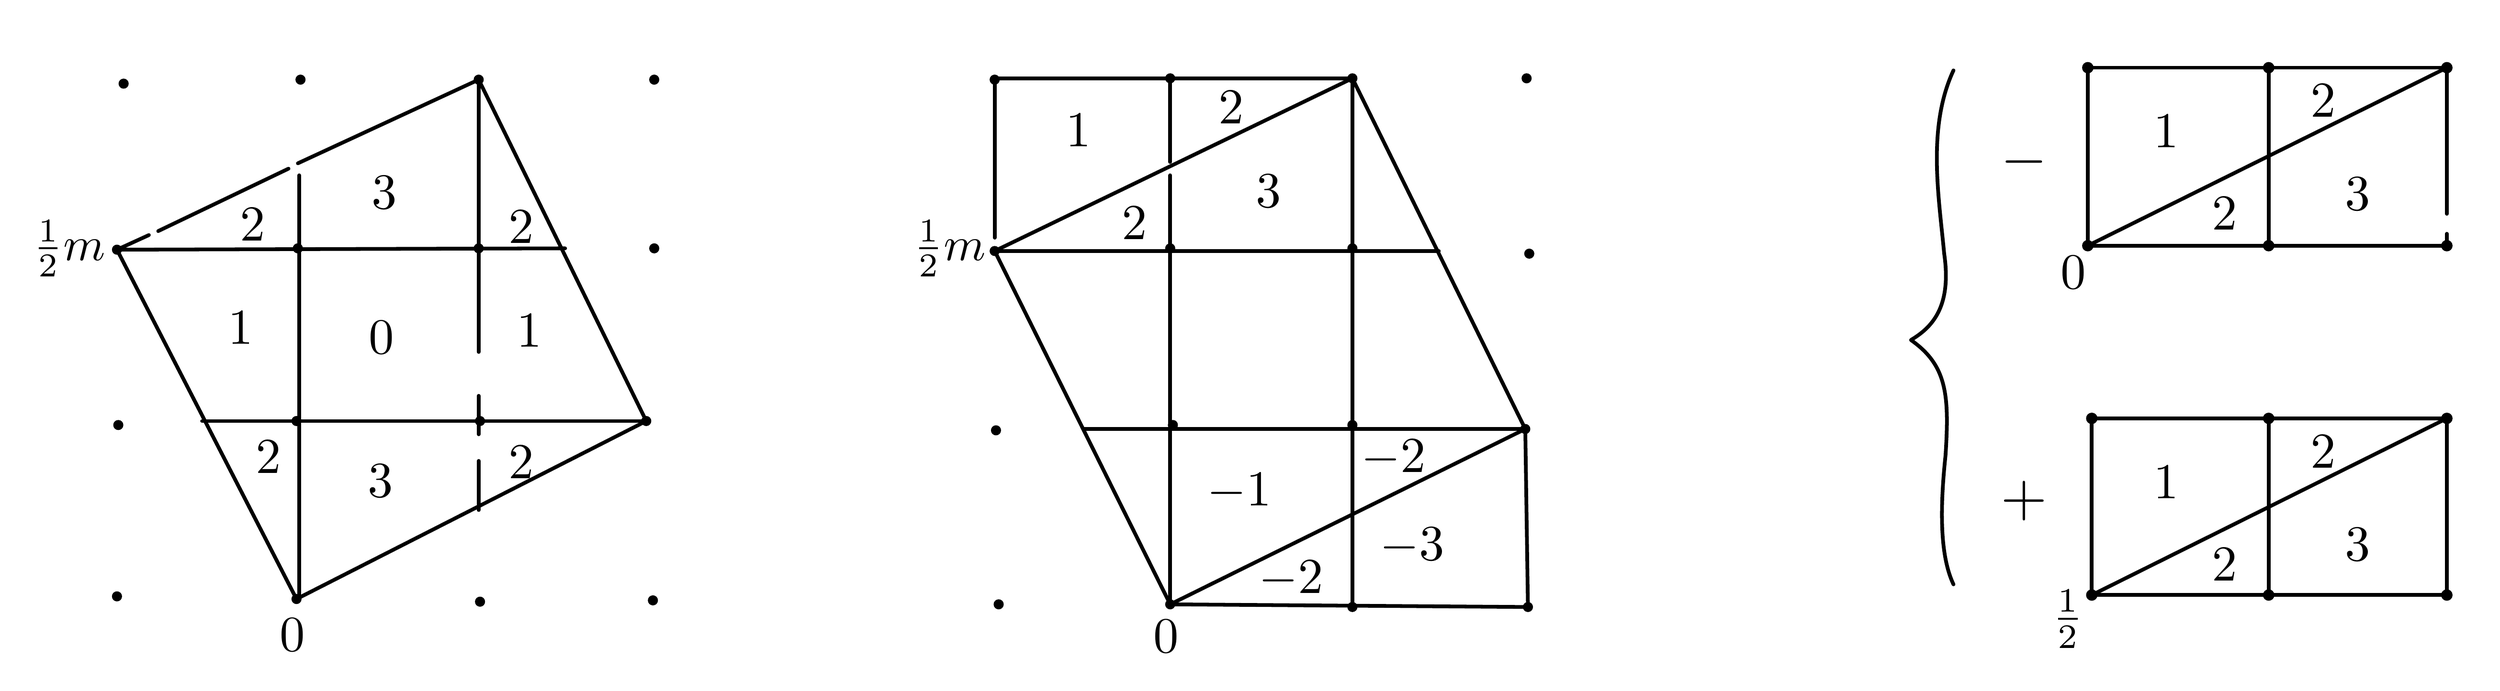
\begin{tikzpicture}[x=1bp,y=-1bp,line cap=round,line join=round]
\path[use as bounding box] (0,0) rectangle (1860,500);
\begin{pgfinterruptboundingbox}
\draw[line width=2.8bp] (78,178) -- (102,167);
\draw[line width=2.8bp] (109,164) -- (207,117);
\draw[line width=2.8bp] (214,113) -- (350,50) -- (476,307) -- (213,441) -- (78,178);
\draw[line width=2.8bp] (215,122) -- (215,441);
\draw[line width=2.8bp] (350,50) -- (350,255);
\draw[line width=2.8bp] (350,288) -- (350,317);
\draw[line width=2.8bp] (350,337) -- (350,374);
\draw[line width=2.8bp] (78,178) -- (415,177);
\draw[line width=2.8bp] (142,307) -- (476,307);
\fill (83,53) circle[radius=3.8bp];
\fill (216,50) circle[radius=3.8bp];
\fill (350,50) circle[radius=3.8bp];
\fill (482,50) circle[radius=3.8bp];
\fill (78,178) circle[radius=3.8bp];
\fill (214,177) circle[radius=3.8bp];
\fill (350,177) circle[radius=3.8bp];
\fill (482,177) circle[radius=3.8bp];
\fill (79,310) circle[radius=3.8bp];
\fill (213,307) circle[radius=3.8bp];
\fill (351,307) circle[radius=3.8bp];
\fill (476,307) circle[radius=3.8bp];
\fill (78,439) circle[radius=3.8bp];
\fill (213,441) circle[radius=3.8bp];
\fill (351,443) circle[radius=3.8bp];
\fill (481,442) circle[radius=3.8bp];
\node[inner sep=0pt,outer sep=0pt,anchor=center] at (180,159) {\scalebox{3.8}{\ensuremath{2}}};
\node[inner sep=0pt,outer sep=0pt,anchor=center] at (279,135) {\scalebox{3.8}{\ensuremath{3}}};
\node[inner sep=0pt,outer sep=0pt,anchor=center] at (382,161) {\scalebox{3.8}{\ensuremath{2}}};
\node[inner sep=0pt,outer sep=0pt,anchor=center] at (171,237) {\scalebox{3.8}{\ensuremath{1}}};
\node[inner sep=0pt,outer sep=0pt,anchor=center] at (277,244) {\scalebox{3.8}{\ensuremath{0}}};
\node[inner sep=0pt,outer sep=0pt,anchor=center] at (388,239) {\scalebox{3.8}{\ensuremath{1}}};
\node[inner sep=0pt,outer sep=0pt,anchor=center] at (192,334) {\scalebox{3.8}{\ensuremath{2}}};
\node[inner sep=0pt,outer sep=0pt,anchor=center] at (276,352) {\scalebox{3.8}{\ensuremath{3}}};
\node[inner sep=0pt,outer sep=0pt,anchor=center] at (382,338) {\scalebox{3.8}{\ensuremath{2}}};
\node[inner sep=0pt,outer sep=0pt,anchor=center] at (42,177) {\scalebox{3.6}{\ensuremath{\frac12 m}}};
\node[inner sep=0pt,outer sep=0pt,anchor=center] at (210,468) {\scalebox{3.8}{\ensuremath{0}}};
\draw[line width=2.8bp] (738,179) -- (1007,49) -- (1137,313) -- (870,445) -- cycle;
\draw[line width=2.8bp] (738,169) -- (738,49) -- (1007,49);
\draw[line width=2.8bp] (870,445) -- (1139,447) -- (1137,313);
\draw[line width=2.8bp] (870,49) -- (870,112);
\draw[line width=2.8bp] (870,122) -- (870,445);
\draw[line width=2.8bp] (1007,49) -- (1007,447);
\draw[line width=2.8bp] (738,179) -- (1072,179);
\draw[line width=2.8bp] (805,313) -- (1137,313);
\fill (738,50) circle[radius=3.8bp];
\fill (870,49) circle[radius=3.8bp];
\fill (1007,49) circle[radius=3.8bp];
\fill (1138,49) circle[radius=3.8bp];
\fill (738,179) circle[radius=3.8bp];
\fill (870,177) circle[radius=3.8bp];
\fill (1007,177) circle[radius=3.8bp];
\fill (1140,181) circle[radius=3.8bp];
\fill (739,314) circle[radius=3.8bp];
\fill (872,310) circle[radius=3.8bp];
\fill (1007,310) circle[radius=3.8bp];
\fill (1137,313) circle[radius=3.8bp];
\fill (741,445) circle[radius=3.8bp];
\fill (870,445) circle[radius=3.8bp];
\fill (1007,447) circle[radius=3.8bp];
\fill (1139,447) circle[radius=3.8bp];
\node[inner sep=0pt,outer sep=0pt,anchor=center] at (801,88) {\scalebox{3.8}{\ensuremath{1}}};
\node[inner sep=0pt,outer sep=0pt,anchor=center] at (843,158) {\scalebox{3.8}{\ensuremath{2}}};
\node[inner sep=0pt,outer sep=0pt,anchor=center] at (916,71) {\scalebox{3.8}{\ensuremath{2}}};
\node[inner sep=0pt,outer sep=0pt,anchor=center] at (944,134) {\scalebox{3.8}{\ensuremath{3}}};
\node[inner sep=0pt,outer sep=0pt,anchor=center] at (922,360) {\scalebox{3.8}{\ensuremath{-1}}};
\node[inner sep=0pt,outer sep=0pt,anchor=center] at (961,426) {\scalebox{3.8}{\ensuremath{-2}}};
\node[inner sep=0pt,outer sep=0pt,anchor=center] at (1038,335) {\scalebox{3.8}{\ensuremath{-2}}};
\node[inner sep=0pt,outer sep=0pt,anchor=center] at (1052,401) {\scalebox{3.8}{\ensuremath{-3}}};
\node[inner sep=0pt,outer sep=0pt,anchor=center] at (704,177) {\scalebox{3.6}{\ensuremath{\frac12 m}}};
\node[inner sep=0pt,outer sep=0pt,anchor=center] at (867,469) {\scalebox{3.8}{\ensuremath{0}}};
\draw[line width=2.8bp] (1459,43) .. controls (1439,86) and (1448,138) .. (1452,181) .. controls (1458,222) and (1442,237) .. (1427,246) .. controls (1454,265) and (1456,287) .. (1453,333) .. controls (1448,380) and (1450,411) .. (1459,430);
\draw[line width=2.8bp] (1830,151) -- (1830,41) -- (1560,41) -- (1560,175) -- (1830,175) -- (1830,166);
\draw[line width=2.8bp] (1696,41) -- (1696,175);
\draw[line width=2.8bp] (1560,175) -- (1830,41);
\fill (1560,41) circle[radius=4.3bp];
\fill (1696,41) circle[radius=4.3bp];
\fill (1830,41) circle[radius=4.3bp];
\fill (1560,175) circle[radius=4.3bp];
\fill (1696,175) circle[radius=4.3bp];
\fill (1830,175) circle[radius=4.3bp];
\node[inner sep=0pt,outer sep=0pt,anchor=center] at (1619,89) {\scalebox{3.8}{\ensuremath{1}}};
\node[inner sep=0pt,outer sep=0pt,anchor=center] at (1663,151) {\scalebox{3.8}{\ensuremath{2}}};
\node[inner sep=0pt,outer sep=0pt,anchor=center] at (1737,66) {\scalebox{3.8}{\ensuremath{2}}};
\node[inner sep=0pt,outer sep=0pt,anchor=center] at (1763,136) {\scalebox{3.8}{\ensuremath{3}}};
\draw[line width=2.8bp] (1563,305) -- (1830,305) -- (1830,438) -- (1563,438) -- cycle;
\draw[line width=2.8bp] (1696,305) -- (1696,438);
\draw[line width=2.8bp] (1563,438) -- (1830,305);
\fill (1563,305) circle[radius=4.3bp];
\fill (1696,305) circle[radius=4.3bp];
\fill (1830,305) circle[radius=4.3bp];
\fill (1563,438) circle[radius=4.3bp];
\fill (1696,438) circle[radius=4.3bp];
\fill (1830,438) circle[radius=4.3bp];
\node[inner sep=0pt,outer sep=0pt,anchor=center] at (1619,353) {\scalebox{3.8}{\ensuremath{1}}};
\node[inner sep=0pt,outer sep=0pt,anchor=center] at (1663,415) {\scalebox{3.8}{\ensuremath{2}}};
\node[inner sep=0pt,outer sep=0pt,anchor=center] at (1737,330) {\scalebox{3.8}{\ensuremath{2}}};
\node[inner sep=0pt,outer sep=0pt,anchor=center] at (1763,400) {\scalebox{3.8}{\ensuremath{3}}};
\node[inner sep=0pt,outer sep=0pt,anchor=center] at (1512,112) {\scalebox{4.5}{\ensuremath{-}}};
\node[inner sep=0pt,outer sep=0pt,anchor=center] at (1512,367) {\scalebox{4.5}{\ensuremath{+}}};
\node[inner sep=0pt,outer sep=0pt,anchor=center] at (1549,195) {\scalebox{3.8}{\ensuremath{0}}};
\node[inner sep=0pt,outer sep=0pt,anchor=center] at (1545,456) {\scalebox{3.7}{\ensuremath{\frac12}}};
\end{pgfinterruptboundingbox}
\end{tikzpicture}
}\end{center}

% A544-P0332-D05
Der Kürze wegen bezeichnen wir $S(x,x+\alpha,x+\alpha+\beta,x+\beta)$ durch $[x,\alpha,\beta]$ so dass
\[
\begin{aligned}
[x,\alpha,\beta]&=-[x,\beta,\alpha]=[x+\alpha,\beta,-\alpha]\\
&=-[x+\alpha,-\alpha,\beta]\\
&=[x+\alpha+\beta,-\alpha,-\beta]\\
&=-[x+\alpha+\beta,-\beta,-\alpha]
\end{aligned}
\]

% A544-P0332-D06
Setzt man ferner
\[
\frac{m}{-2-4i}=\frac{-a-2b}{10}+\frac{-b+2a}{10}i=Q
\]
\SourceLeaf{333}%
% A544-P0333-D01
so besteht der Decident aus folgenden acht Theilen
\[
\begin{aligned}
\mathrm{I}&=[0,\tfrac12,-iQ]\\
-2\mathrm{II}&=-2[0,\tfrac12,Q]\\
\mathrm{III}&=+[Q,\tfrac12,-iQ]\\
\mathrm{IV}&=+[-iQ,\tfrac12,Q]\\
-3\mathrm{V}&=-3[Q,\tfrac12,Q]\\
-3\mathrm{VI}&=-3[2Q,\tfrac12,-iQ]\\
+2\mathrm{VII}&=+2[(1-i)Q,\tfrac12,Q]\\
+\mathrm{VIII}&=+[0,\tfrac12,\tfrac12im]
\end{aligned}
\]

% A544-P0333-D02
Ist $F$ indefinite ein Elementarrest des Modulus $-1-2i$, so hat man
\[
\Sigma[2FQ,\tfrac12,iQ]=[0,-\tfrac12-i,\tfrac12im]
\]

% A544-P0333-D03
Setzt man also für $F$: $0,1,i,-1,-i$ so hat man
\[
\begin{array}{rll}
0={}&[0,\tfrac12,iQ]&=\mathrm{IX}\\
&+[2Q,\tfrac12,iQ]&=\mathrm{X}\pdot\\
&+[2iQ,\tfrac12,iQ]&=\mathrm{XI}\\
&+[-2Q,\tfrac12,iQ]&=\mathrm{XII}\\
&+[-2iQ,\tfrac12,iQ]&=\mathrm{XIII}\\
&-[0,-\tfrac12-i,\tfrac12im]&=-\mathrm{XIV}
\end{array}
\]

% A544-P0333-D04
Man setze dies zu dem vorigen Werth des Decident hinzu. Aus dieser Vereinigung fliessen folgende Resultate

% A544-P0333-D05
(1) Da $(1+2i)Q+\frac12$ eine ganze Zahl ist, so wird
\[
\begin{aligned}
\mathrm{XI}&=[-Q-\tfrac12,\tfrac12,iQ]= -[-Q,-\tfrac12,iQ]\\
&=-[Q,\tfrac12,-iQ]
\end{aligned}
\]
also
\[
\mathrm{III}+\mathrm{XI}=0
\]

% A544-P0333-D06
(2) Wir ziehen zusammen $\mathrm{IV},-3\mathrm{V},\mathrm{X},\mathrm{XIII}$ auf folgende Weise
\[
\begin{aligned}
\mathrm{IV}&=+[-2Q+\tfrac12i,\tfrac12,Q]=[-2iQ-\tfrac12,\tfrac12i,iQ]\\
\mathrm{V}'&=-[2Q,+\tfrac12,-Q]=-[-2iQ,-\tfrac12i,iQ]\\
\mathrm{X}&=[+iQ-\tfrac12i,\tfrac12,iQ]\\
&=[-iQ+\tfrac12i,-\tfrac12,-iQ]=[-2iQ-\tfrac12+\tfrac12i,\tfrac12,iQ]\\
\mathrm{XIII}&=[-2iQ,\tfrac12,iQ]
\end{aligned}
\]

\SourceLeaf{334}%
% A544-P0334-D01
Also die ganze Ausbeute aus diesen Theilen
\[
\begin{aligned}
&-4\mathrm{V}\\
&+R(-2iQ)-R(-iQ)-I(-2iQ)+I(-iQ)\\
&-\text{Quadr. }[-2iQ-\tfrac14+\tfrac14i]\\
&+\text{Quadr. }[-2iQ+\tfrac14-\tfrac14i]
\end{aligned}
\]

% A544-P0334-D02
(3) $\mathrm{I},-2\mathrm{II},-3\mathrm{VI},+2\mathrm{VII},+\mathrm{IX},+\mathrm{XII}$ zusammengezogen geben folgendes
\[
\begin{aligned}
\mathrm{I}&=[0,\tfrac12,-iQ]\\
\mathrm{II}&=[0,-\tfrac12i,-iQ]\\
\mathrm{VI}&=[iQ-\tfrac12i,\tfrac12,-iQ]=[\tfrac12-\tfrac12i,-\tfrac12,iQ]\\
&=[-\tfrac12+\tfrac12i,\tfrac12,-iQ]\\
\mathrm{VII}&=[-Q-\tfrac12i,\tfrac12,Q]=[-\tfrac12+\tfrac12i,-\tfrac12,-Q]\\
&=[+\tfrac12+\tfrac12i,-\tfrac12i,-iQ]\\
\mathrm{IX}&=[0,-\tfrac12,-iQ]\\
\mathrm{XII}&=[-iQ+\tfrac12i,\tfrac12,iQ]=[\tfrac12+\tfrac12i,-\tfrac12,-iQ]
\end{aligned}
\]
\[
\begin{aligned}
={}&+4\mathrm{I}-4\mathrm{II}-4\mathrm{VI}+4\mathrm{XII}\\
&-I(\tfrac12i)+I(-iQ+\tfrac12i)+I0-I(-iQ)-2R0+2R(-iQ)\\
&+2\text{Quadr. }(-iQ+\tfrac14+\tfrac14i)\\
={}&4\mathrm{I}-4\mathrm{II}-4\mathrm{VI}+4\mathrm{XII}\\
&+R(-1-2i)Q-R(-2iQ)-I(-iQ)+2R(-iQ)\\
&+2\text{Quadr. }(-2iQ+\tfrac14+\tfrac14i)
\end{aligned}
\]

% A544-P0334-D03
Dies Alles zusammen gibt folglich
\[
\begin{aligned}
&+4\mathrm{I}-4\mathrm{II}-4\mathrm{V}-4\mathrm{VI}+4\mathrm{XII}+\tfrac12(a-1)-\tfrac12b\\
&+\text{Quadr. }(-2iQ+\tfrac14-\tfrac14i)\\
&+2\text{Quadr. }(-2iQ+\tfrac14+\tfrac14i)\\
&-\text{Quadr. }(-2iQ-\tfrac14+\tfrac14i)
\end{aligned}
\]

% A544-P0334-D04
Endlich gibt $\mathrm{VIII}-\mathrm{XIV}=\frac12(a-1)+\frac12b$
Also da die drei Quadrattheile dem Decident von $\frac{m}{-1-2i}$ gleich sind, so wird
\[
\text{Dec. }\frac{-1-2i}{m}\equiv a-1+\text{Dec. }\frac{m}{-1-2i}\quad\text{W. Z. B. W.}
\]

% A544-P0334-D05
Wahrscheinlich wird der Beweis noch sehr dadurch vereinfacht werden können, dass
\[
\text{Dec. }\frac{1+2i}{m}=\vcenter{\hbox{\resizebox{.35\textwidth}{!}{\begin{tikzpicture}[x=1bp,y=-1bp,line cap=round,line join=round]
\path[use as bounding box] (0,0) rectangle (620,220);
\begin{pgfinterruptboundingbox}
\draw[line width=2.1bp] (147,35) -- (485,32) -- (213,173) -- cycle;
\node[inner sep=0pt,outer sep=0pt,anchor=east] at (138,34) {\scalebox{2.6}{\ensuremath{\frac12(1+i)m}}};
\node[inner sep=0pt,outer sep=0pt,anchor=west] at (494,32) {\scalebox{2.6}{\ensuremath{(-1+i)m}}};
\node[inner sep=0pt,outer sep=0pt,anchor=center] at (205,194) {\scalebox{3.6}{\ensuremath{0}}};
\end{pgfinterruptboundingbox}
\end{tikzpicture}
}}}
\]

\SourceLeaf{335}%
% A544-P0335-D01
\Article{19}
Durch Induction ist folgendes gefunden
\[
\begin{aligned}
\text{Dec. }\frac{a-bi}{a+bi}&\equiv\frac{aa+2ab-1}{4},& a&\equiv1\ (\mathrm{mod.}\ 4)\\
&\equiv\frac{aa+2ab+2bb-1}{4},&a+bi&\equiv1\ (\mathrm{mod.}\ 2+2i)
\end{aligned}
\]

% A544-P0335-D02
Hiemit steht Folgendes in Verbindung:
Es sei $aa+bb=p$ (Primzahl) $a\equiv1\ (\mathrm{mod.}\ 4)$
\[
\begin{aligned}
1\pdot2\pdot3\mathinner{.\,.\,.\,.\,.\,.\,.\,.\,.\,.\,.}\tfrac14(p-1)&\equiv\alpha\ \mathrm{mod.}p\\
\tfrac14(p+3)\pdot\tfrac14(p+7)\ldots\tfrac12(p-1)&\equiv\beta\\
\tfrac12(p+1)\pdot\tfrac12(p+3)\ldots\tfrac34(p-1)&\equiv\gamma\\
\tfrac14(3p+1)\mathinner{.\,.\,.\,.\,.\,.\,.\,.\,.}\ p-1&\equiv\delta
\end{aligned}
\]
so ist
\[
\begin{aligned}
\alpha&\equiv\delta,&\beta&\equiv\gamma&\text{wenn }\tfrac12b\text{ gerade}\\
\alpha&\equiv-\delta,&\beta&\equiv-\gamma&\text{wenn }\tfrac12b\text{ ungerade}
\end{aligned}
\]
\[
\begin{gathered}
\pm\alpha\beta\equiv i,\quad\pm\beta\beta\equiv2b,\quad\frac\beta\alpha\equiv2a,\\
\frac\beta{1+\alpha\beta}\equiv\surd a,\quad\tfrac12\beta(1-\alpha\beta)\equiv\surd a
\end{gathered}
\]

% A544-P0335-D03
Es wird demnach nur darauf ankommen die Decidenten bei reellen Resten zu bestimmen
\[
\begin{gathered}
a^{\frac14bb}\pdot b^{\frac14(aa-1)}\equiv1\ (\mathrm{mod.}\ (aa+bb))\\
\text{si }a\equiv1)(\mathrm{mod.}\ 4)\quad b\text{ par}\quad aa+bb\text{ primus}
\end{gathered}
\]

% A544-P0335-D04
Will man bloss mit reellen Zahlen zu thun haben, so kommt es auf folgendes Haupttheorem an. Es sei $a-1$ durch $4$, $b$ durch $2$ theilbar; $a$ und $b$ ohne gemeinschaftlichen Divisor, $k$ bedeute die Zahlen $1,2,3\ldots aa+bb-1$.
Es sei
\begin{list}{}{\setlength{\labelwidth}{1.5em}\setlength{\leftmargin}{2em}}
\item[$\alpha$] die Zahl aller Werthe von $k$, wo die kleinsten Reste von $ak,\allowbreak bk,\quad\allowbreak aak,\quad\allowbreak abk$ alle zwischen $0$ und $\frac12(aa+bb)$ liegen
\item[$\beta$] $ak,bk,\quad aak,-abk$
\item[$\gamma$] $ak,bk,-aak,-abk$
\item[$\delta$] $ak,bk,-aak,\quad abk$
\end{list}
alsdann ist $\beta+2\gamma+3\delta-\frac14(aa-1)$ durch $4$ theilbar.
\BookRule{.35\textwidth}


\SourceLeaf{336}%
% A544-P0336-D01
\section*{[II.]}
\begin{center}VORBEREITUNGEN ZUR ALLGEMEINEN THEORIE\\DER BIQUADRATISCHEN RESTE.\end{center}
\pdfbookmark[1]{II. Vorbereitungen zur allgemeinen Theorie der biquadratischen Reste}{nachlass-biquadratic-II}
\BookRule{.15\textwidth}
\par\medskip\pdfbookmark[2]{(1.)}{nachlass-biquadratic-II-prefatory-1}\centerline{(1.)}\smallskip
Es sei $P=x+iy$, wo weder $x$ noch $y$ eine ganze Zahl ist. Wir bezeichnen die. Zahl $+1$ durch $LP,L'P,L''P,L'''P$, je nachdem $P$ im ersten, zweiten, dritten oder vierten Quadranten liegt (im ersten und zweiten Quadranten ist $[y]$ gerade, im dritten und vierten ungerade; im ersten und vierten ist $[x]$ gerade, im zweiten und dritten ungerade). In allen Fällen, wo diese Zeichen nicht $=1$ sind, werden sie $=0$ vorausgesetzt. Man hat dann folgende $24$ Relationen

% A544-P0336-D02
\[
\begin{array}{lll}
L(P\pm1)=L'P&L(P\pm i)=L'''P&L(P\pm1\pm i)=L''P\\
L'(P\pm1)=LP&L'(P\pm i)=L''P&L'(P\pm1\pm i)=L'''P\\
L''(P\pm1)=L'''P&L''(P\pm i)=L'P&L''(P\pm1\pm i)=LP\\
L'''(P\pm1)=L''P&L'''(P\pm i)=LP&L'''(P\pm1\pm i)=L'P
\end{array}
\]
\[
\begin{array}{lll}
LiP=L'''P&L(-P)=L''P&L(-iP)=L'P\\
L'iP=LP&L'(-P)=L'''P&L'(-iP)=L''P\\
L''iP=L'P&L''(-P)=LP&L''(-iP)=L'''P\\
L'''iP=L''P&L'''(-P)=L'P&L'''(-iP)=LP
\end{array}
\]

% A544-P0336-D03
\par\medskip\pdfbookmark[2]{(2.)}{nachlass-biquadratic-II-prefatory-2}\centerline{(2.)}\smallskip
Durch $PP'$ oder $z$ bezeichnen wir eine Linie, die von $P$ anfängt und in $P'$ endigt. Sie braucht nicht gerade zu sein. Wir legen allen geraden Linien von $2x+2iy$ nach $2x+(2y+1)i$ gezogen (wo $x,y$ indefinite alle ganzen Zahlen bedeuten) eine positive und eine negative Seite bei; für jene wählen wir die rechte, für diese die linke. Durch $Tz$ bezeichnen wir die Anzahl aller Schnitte
\SourceLeaf{337}%
% A544-P0337-D01
der Linie $z$ mit den eben gedachten Linien, als positiv gezählt diejenigen, wo $z$ von der negativen Seite auf die positive übergeht, als negativ die andern. Ferner setzen wir
\[
Tz-T(z-1)=Sz
\]

% A544-P0337-D02
($z-1$ ist eine der $z$ parallele Linie, die von dem Punkte $P-1$ nach $P'-1$ geht). Offenbar brauchen wir nur dem oben gedachten System von Linien noch die von $2x+1+2yi$ nach $2x+1+(2y+1)i$ gezogenen beizufügen und deren linke Seiten positiv und die rechten als negativ zu betrachten, um in $Sz$ die Anzahl aller Schnitte von $z$ mit diesem zweifachen System von Geraden zu erkennen. Wir haben nun ferner
\[
\begin{aligned}
T(-z)&=-T(z+i)\\
T(z)+T(z+i)&=[\tfrac12x]-[\tfrac12x']\\
S(z+1)&=-Sz\\
S(z+i)&=-Sz+LP+L'''P-LP'-L'''P'\\
S(z+1+i)&=Sz-LP+L'''P+LP'+L'''P'\\
Siz&=Sz-LP+LP'\\
S(-z)&=Sz-LP-L'''P+LP'+L'''P'\\
S(-iz)&=Sz+L'P-L'P'
\end{aligned}
\]

% A544-P0337-D03
\renewcommand{\Article}[1]{\par\medskip\Needspace{4\baselineskip}\pdfbookmark[2]{Art. #1}{nachlass-biquadratic-II-art-#1}\centerline{\textbf{#1.}}\nobreak\smallskip}
\Article{1}
Wir betrachten in der Ebene zwei Gattungen von Punkten; einmal die, denen ganze Zahlen entsprechen; dann diejenigen, welche durch Producte aus ganzen Zahlen in die Grösse $Q=\frac{m}{2M}$ bestimmt werden. Wir können dieselben durch die Benennungen Punkte der ersten und Punkte der zweiten Ordnung unterscheiden.

% A544-P0337-D04
\Article{2}
Indem wir jeden Punkt der zweiten Ordnung mit seinen vier Nachbarn durch gerade Linien verbinden, die wir \emph{Ligaturen} nennen werden, theilt sich die ganze Ebene in unendlich viele Quadrate. Die Punkte der ersten Ordnung liegen theils innerhalb dieser Quadrate, theils auf den Ligaturen innerhalb der 
\SourceLeaf{338}%
% A544-P0338-D01
Grenzen derselben, theils auf den Grenzen der Ligaturen, das letzte, wenn sie zugleich Punkte der zweiten Ordnung sind. Ist $kQ$ ein solcher Punkt, so muss insofern $m,M$ ohne gemeinschaftlichen Theiler und beide ungerade sind, $k$ durch $M$ theilbar sein.

% A544-P0338-D02
\Article{3}
Bei den Ligaturen können wir zugleich einen Unterschied zwischen dem Anfangspunkte und Endpunkte machen, also $PQ$ von $QP$ unterscheiden, oder auch in einigen Fällen diesen Unterschied bei Seite setzen. Wir nennen zwei solche Ligaturen entgegengesetzte. Bezeichnen können wir überhaupt am bequemsten die Ligaturen durch ihren Anfangs- und Endpunkt, die man allenfalls in eine Klammer einschliessen mag. Einer Ligatur entgegengesetzte soll durch das doppelte Ueberstreichen angedeutet werden $QP=\overline{\overline{PQ}}$.

% A544-P0338-D03
\Article{4}
Jedes der gedachten Quadrate wird von vier solchen Ligaturen einge\-schlossen
\[
\begin{gathered}
\{kQ,(k+1)Q\},\ \{(k+1)Q,(k+1+i)Q\},\\
\{(k+1+i)Q,(k+i)Q\},\ \{(k+i)Q,kQ\}\dotsfour\Omega
\end{gathered}
\]
denen es zur rechten liegt. Es ist wichtig hiebei auf die Form der Zahl $k$ zu sehen, und wir unterscheiden in dieser Beziehung viererlei Quadrate, je nachdem $k\equiv0,1,1+i,i\ (\mathrm{mod.}\ 2)$ ist, und bedienen uns dann der Zahlen $0,1,2,3$, die wir resp. die Intensoren der Quadrate nennen.

% A544-P0338-D04
\Article{5}
Den Ligaturen legen wir dieselben Intensoren bei, welche die ihnen zur rechten liegenden Quadrate haben.

% A544-P0338-D05
\Article{6}
Wir haben nun ein anderes grösseres Quadrat $\Omega'$ zu betrachten, nemlich dasjenige. welches entsteht, wenn das in $4$ angezeigte für $k=0$, mit $M$ multiplicirt wird: dies wird also durch die geraden Linien $\mu,\mu',\mu'',\mu'''$ begrenzt
\[
\{0,\tfrac12m\},\ \{\tfrac12m,\tfrac12(1+i)m\},\ \{\tfrac12(1+i)m,\tfrac12im\},\ \{\tfrac12im,0\}
\]
Es besteht aus ganzen Quadraten $\Omega$ und Stücken solcher Quadrate; man zähle
\SourceLeaf{339}%
% A544-P0339-D01
alle Punkte der ersten Ordnung innerhalb desselben zusammen, indem man für jeden Punkt den Intensor des Quadrats $\Omega$, worin er liegt, nimmt, diese Summe oder deren kleinster Rest nach dem Modulus $4$ heisst der Decident von $M$ für den Modulus $m$, und bestimmt die biquadratische Modalität von $M$ in Beziehung auf diesen Modulus.

% A544-P0339-D02
\Article{7}
Wir zerlegen das Quadrat $\Omega'$ in $5$ Stücke auf folgende Art. Man verbinde den Punkt $0$ mit $\frac14(1+i)(m-1)$ durch die Linie $\lambda$, die durch lauter Ligaturen innerhalb $\Omega'$ gehe. Es sei
\[
\tfrac12m+i\lambda=\lambda',\quad\tfrac12(1+i)m-\lambda=\lambda'',\quad\tfrac12im-i\lambda=\lambda'''
\]
diese $4$ Linien gehen also von den Ecken des Quadrats $\Omega'$ aus ins Innere und endigen sich an den vier Ecken des innersten Quadrats, dessen Intensor $0$ sein wird, wenn $m\equiv1\ (\mathrm{mod.}\ 2+2i)$; die Ligaturen dieses Quadrats seien $\nu,\nu',\nu'',\nu'''$.

% A544-P0339-D03
Die $5$ Stücke werden also begrenzt sein
\[
\begin{array}{rll}
\mathrm{I}.&\ldots&\mu,\ \lambda',\ \overline{\overline\nu},\ \overline{\overline\lambda}\\
\mathrm{II}.&\ldots&\mu',\ \lambda'',\ \overline{\overline{\nu'}},\ \overline{\overline{\lambda'}}\\
\mathrm{III}.&\ldots&\mu'',\ \lambda''',\ \overline{\overline{\nu''}},\ \overline{\overline{\lambda''}}\\
\mathrm{IV}.&\ldots&\mu''',\ \lambda,\ \overline{\overline{\nu'''}},\ \overline{\overline{\lambda'''}}\\
\mathrm{V}.&\multicolumn{2}{l}{\text{das innere Quadrat }\nu,\ \nu',\ \nu'',\ \nu'''}
\end{array}
\]
Der Decident ist also die Aufzählung aller Punkte erster Ordnung in I. II. III. IV.

% A544-P0339-D04
\Article{8}
Der Kürze wegen soll Intensor irgend eines Punkts der Intensor des Quadrats sein, in dem er liegt, und durch vorgesetztes $\Upsilon$ ausgedrückt werden.

% A544-P0339-D05
\Article{9}
Der Decident ist also
\[
\Sigma\Upsilon P+\Sigma\Upsilon P'+\Sigma\Upsilon P''+\Sigma\Upsilon P'''
\]
wo $P$ alle Punkte in I. u. s. w. bedeuten.

\SourceLeaf{340}%
% A544-P0340-D01
\Article{10}
Wir betrachten nun noch den Raum $\mathrm{VI}=-i\mathrm{IV}$, welcher ausserhalb $\Omega'$ liegt, sich aber durch $\mu$ an I anschliesst und mit ihm zusammen den Raum $\omega$ ausmacht, der aus $AA+BB$ vollständigen Quadraten besteht. Bedeutet $\Pi$ alle ganzen; $\Pi'$ alle um $\frac12i$ vermehrten ganzen Punkte dieses Raumes, so lässt sich leicht beweisen, dass der Decident
\[
\begin{aligned}
={}&\Sigma\Upsilon\Pi-\Sigma\Upsilon\Pi'+\text{Anzahl aller ganzen Punkte innerhalb VI}\\
&-\text{Anzahl aller halben Punkte innerhalb VI.}
\end{aligned}
\]

% A544-P0340-D02
\Article{11}
Man denke sich von jedem ganzen Punkte $k$ nach $k+\frac12i$ gerade Linien gezogen, deren rechte Seite als positiv, die linke als negativ angesehen wird. Es sei $l$ eine Linie, und $Sl$ bezeichne die Summe aller Schnitte der $l$ mit jenem System von Linien, diejenigen als positiv angesehen, wo $l$ von der negativen auf die positive übergeht, die entgegengesetzten Schnitte als negativ. Man hat dann für den Decidenten folgenden Ausdruck
\[
\Sigma(\Upsilon l\pdot Sl)+\Sigma Sl'-S\mu
\]

% A544-P0340-D03
wo $l$ alle Ligaturen der Quadrate in $\omega$ bedeuten (immer so genommen, dass die Quadrate ihnen zur rechten liegen) und wo $l'$ diejenigen Ligaturen bedeutet, die auf dem Umfange der Figur $\omega$ zwischen $0$ und $\frac12m$ liegen, also ausserhalb $\Omega'$.

% A544-P0340-D04
Alle Ligaturen $l$ bestehen aus
\begin{enumerate}
\item[1)] $l'$
\item[2)] $l''$ die innerhalb $\Omega'$ liegenden Grenzligaturen also $\lambda',\overline{\overline\nu},\overline{\overline\lambda}$.
\item[3)] $l'''$ die im Innern von $\omega$ liegen.
\end{enumerate}
Verstände man unter $l$ indefin. alle Ligaturen, die sich innerhalb $\omega$ oder auf den Grenzen dieser Figur befinden, insofern sie von Punkten $\frac{km}{2M}$ ausgehen, so dass $k$ durch $1+i$ theilbar ist, so wäre der Decident
\[
=\Sigma\alpha\pdot Sl-S\mu
\]

% A544-P0340-D05
\begin{list}{}{\setlength{\labelwidth}{5em}\setlength{\leftmargin}{5.5em}}
\item[wo $\alpha=1$] für alle Ligaturen im Innern von $\omega$
\item[$\alpha=\Upsilon l+1$] für alle Grenzligaturen ausserhalb $\Omega'$, deren Richtung in der von $0$ nach $\frac12m$ gehenden Grenze liegt
\end{list}


\SourceLeaf{341}%
% A544-P0341-D01
\begin{list}{}{\setlength{\labelwidth}{9em}\setlength{\leftmargin}{9.5em}}
\item[$\alpha=-(\Upsilon\overline{\overline\lambda}+1)=-\Upsilon l$] für alle auf dieser Grenze, die in entgegengesetztem Sinne laufen
\item[$\alpha=\Upsilon l$] für alle Grenzligaturen innerhalb $\Omega'$, deren Richtung auf $0$ zugeht
\item[$\alpha=-\Upsilon l+1$] für alle Grenzligaturen innerhalb $\Omega'$, deren Richtung von $0$ abwärts geht.
\end{list}

% A544-P0341-D02
\Article{12}
Wir können nun die sämmtlichen vorkommenden $l$ (nach der letzten Manier) zu zweien combiniren, nemlich $l$ mit $\overline{\overline{\frac12m-l}}$, welche wir verbundene Ligaturen nennen wollen; eine einzige ist hiervon ausgenommen, welche isolirt steht oder mit ihrer verbundenen Ligatur identisch ist, nemlich diejenige, welche von
\[
\tfrac12(M-1)\pdot\frac{m}{2M}\quad\text{nach}\quad\tfrac12(M+1)\frac{m}{2M}\quad\text{läuft}
\]
für verbundene Ligaturen ist das $\alpha$ immer einerlei.
\BookRule{.3\textwidth}

% A544-P0341-D03
\par\bigskip\Needspace{7\baselineskip}
\pdfbookmark[1]{Theorie der biquadratischen Reste. III}{nachlass-biquadratic-III}
\begin{center}[III.]\par\medskip\textsc{Theorie der biquadratischen Reste.}\end{center}
\BookRule{.08\textwidth}
\renewcommand{\Article}[1]{\par\medskip\Needspace{4\baselineskip}\pdfbookmark[2]{Art. #1}{nachlass-biquadratic-III-art-#1}\centerline{\textbf{#1.}}\nobreak\smallskip}
\Article{1}
Kleinste Reste des Modulus $m=a+bi$ heissen die ganzen Zahlen $\mu=\alpha+\beta i$, für welche $\frac{\mu}{m}=x+yi$ so beschaffen ist, dass $x$ und $y$ positiv und kleiner als $1$ sind. Es kommt noch dazu der Rest $0$\begingroup\renewcommand{\thefootnote}{*)}\footnote{und wenn $a$ und $b$ etwa den gemeinschaftlichen Divisor $e$ haben, die Zahlen $\frac{m}{e},\frac{2m}{e},\frac{3m}{e}\dotstwo\frac{(e-1)m}{e}$. Jedoch wollen wir diesen Fall vorerst von der Untersuchung ausschliessen.}\endgroup. Ihre Anzahl ist $=aa+bb$.

% A544-P0341-D04
\Article{2}
In sofern $aa+bb$ ungerade ist, wird $aa+bb$ von der Form $4n+1$ sein. Den kleinsten Rest $0$ ausgeschlossen, theilen sich die übrigen in vier Classen. Zur ersten Classe $f$ zählen wir diejenigen, wo $x$ und $y$ kleiner als $\frac12$ sind,
\SourceLeaf{342}%
% A544-P0342-D01
\[
\begin{array}{lcll}
\text{die zweite}&f'&\text{wo }x>\tfrac12,&y<\tfrac12\\
\text{dritte}&f''&x>\tfrac12,&y>\tfrac12\\
\text{vierte}&f'''&x<\tfrac12,&y>\tfrac12
\end{array}
\]
Man erhält alle Reste
\[
\begin{array}{rcl}
f'&\text{aus}&if+m\\
f''&\text{aus}&-f+(1+i)m\\
f'''&\text{aus}&-if+im
\end{array}
\]

% A544-P0342-D02
\Article{3}
Es sei $M$ eine andere Zahl, die mit $m$ keinen Factor gemein hat, so wird
\[
M^{aa+bb-1}\equiv1\ (\mathrm{mod.}\ m)
\]
sein: folglich $M^{\frac14(aa+bb-1)}$ entweder $\equiv1$, oder $\equiv i$, oder $\equiv-1$, oder $\equiv-i$ d.\,i. $\equiv i^{\varepsilon}$, wo $\varepsilon$ eine der vier Zahlen $0,1,2,3$ vorstellt. Im ersten Fall wird $M$ biquadratischer Rest von $m$ sein, mithin auch quadratischer. Im dritten ist $M$ quadratischer aber nicht biquadratischer Rest; im zweiten und vierten sowohl quadratischer als biquadratischer Nichtrest. Wir nennen dies $\varepsilon$, wovon die biquadratische Modalität der Zahl $M$ in Beziehung auf den Modulus $m$ abhängt, den Decidenten von $M$ beim Modulus $m$. Die Induction lehrt folgenden schönen Lehrsatz. „Sind $M$ und $m$ ungerade Primzahlen von der Form $1+(2+2i)\mu$, so dass $\mu$ eine ganze Zahl ist, so ist die Differenz der beiden Decidenten, von $M$ beim Modulus $m$, und von $m$ beim Modulus $M$ entweder $=0$ oder $=2$; das erstere, wenn wenigstens eine der Zahlen $m,M$ von der Form $1+4N$ ist; das andere, wenn beide von der Form $1+2i+4N$ sind.“ Dies Theorem der Reciprocität ist dem bei den Quadratischen Resten bei blos reellen Zahlen analog.

% A544-P0342-D03
\Article{4}
Man multiplicire alle Zahlen $f$ mit $M$, und suche deren kleinste Reste nach dem Modulus $m$. Es seien darunter
\[
\begin{array}{cll}
\alpha&\text{zu }f&\text{gehörig}\\
\beta&f'&\\
\gamma&f''&\\
\delta&f'''&
\end{array}
\]
so ist $\varepsilon\equiv\beta+2\gamma+3\delta\ (\mathrm{mod.}\ 4)$.

\SourceLeaf{343}%
% A544-P0343-D01
Beweis. Der Inbegriff derjenigen Zahlen aus $f$, deren Producte mit $M$ Reste zu $f$ gehörig geben, sei $g$; der Inbegriff derjenigen, deren Producte Reste aus $f'$ geben, sei $g'$, und ebenso $g''\pdot g'''$; so werden die kleinsten Reste von
\[
-ig'M,\quad -g''M,\quad ig'''M
\]
alle in $f$ enthalten, und sowohl unter sich als von den kleinsten Resten der Producte $gM$ verschieden sein, folglich das Product aus allen
\[
gM,\quad -ig'M,\quad -g''M,\quad +ig'''M
\]
dem Producte aller $f$ congruent sein, mithin auch dem Producte aller $g,g',g'',g'''$. Jenes Product ist aber gleich dem Producte aus allen $g,g',g'',g'''$ in
\[
M^{\alpha}\pdot(-iM)^{\beta}\pdot(-M)^{\gamma}\pdot(iM)^{\delta}
\]
also dies letzte Product $\equiv1$
\[
\begin{aligned}
\text{folglich}\qquad&M^{\alpha+\beta+\gamma+\delta}(-i)^{\beta}(-1)^{\gamma}i^{\delta}\equiv1\\
\text{oder}\qquad&M^{\alpha+\beta+\gamma+\delta}\equiv i^{\beta}(-1)^{\gamma}(-i)^{\delta}\equiv i^{\beta+2\gamma+3\delta}
\end{aligned}
\]
woraus der Lehrsatz von selbst folgt.

% A544-P0343-D02
\Article{5}
Die Entscheidung, ob der kleinste Rest einer Zahl $N$ nach dem Modulus $m$ zur Classe $f,f',f''$ oder $f'''$ gehöre, ist leicht. Ist nemlich $\omega$ die in $\frac{N}{m}$ enthaltene ganze Zahl, so wird jener Rest $=N-\omega m$ sein, und also zu $f,f',f''$ gehören, jenachdem
\[
\frac{N}{m}-\omega=x+iy
\]
gesetzt
\[
\begin{array}{ll}
x<\tfrac12,&y<\tfrac12\\
x>\tfrac12,&y<\tfrac12\\
x>\tfrac12,&y>\tfrac12\\
x<\tfrac12,&y>\tfrac12
\end{array}
\]
ist. In diesen $4$ Fällen wird der Reihe nach die in $\frac{2N}{m}$ enthaltene ganze Zahl folgende sein
\SourceLeaf{344}%
% A544-P0344-D01
\[
\begin{array}{l}
2\omega\\
2\omega+1\\
2\omega+1+i\\
2\omega+i
\end{array}
\]
Hieraus ist klar, dass der kleinste Rest von $N$ nach dem Modulus $m$ zu $f,f',f'',f'''$ gehören werde, je nachdem die in $\frac{2N}{m}$ enthaltene ganze Zahl $=\xi+\eta i$ gesetzt
\[
\begin{array}{ll}
\xi\ \text{gerade}&\eta\ \text{gerade}\\
\xi\ \text{ungerade}&\eta\ \text{gerade}\\
\xi\ \text{ungerade}&\eta\ \text{ungerade}\\
\xi\ \text{gerade}&\eta\ \text{ungerade}
\end{array}
\]

% A544-P0344-D02
\Article{6}
Hienach findet sich der Decident von $M$ nach dem Modulus $m$ auf folgende Art. Man suche die ganzen Zahlen, die in allen einzelnen $\frac{2fM}{m}$ enthalten sind. Diese allgemein durch $x+yi$ bezeichnet, lasse man ganz aus der Acht, diejenigen, wo $x$ und $y$ beide gerade sind, rechne für jede derjenigen, wo $x$ ungerade und $y$ gerade ist, eins, entnehme für jede derjenigen, wo $x$ und $y$ beide ungerade sind, zwei, und drei für jede von denen, wo $x$ gerade, $y$ ungerade ist. Von der Summe aller dieser Zahlen nehme man den kleinsten Rest nach $4$, welcher der verlangte Decident sein wird. Wir drücken dies so aus
\[
\mathrm{Dec.}\frac{M}{m}=\Sigma n
\]
wo $[\frac{2fM}{m}]=x+yi$, $n=0$ zu setzen ist, wenn $x$ gerade $y$ gerade
\[
\begin{array}{cll}
1&x\ \text{ungerade}&y\ \text{gerade}\\
2&x\ \text{ungerade}&y\ \text{ungerade}\\
3&x\ \text{gerade}&y\ \text{ungerade}
\end{array}
\]
Kürze halber wollen wir $n$ durch die Characteristik $\Theta$ bezeichnen, $n=\Theta\frac{2fM}{m}$\begingroup\renewcommand{\thefootnote}{*)}\footnote{Um zu entscheiden, in welche Classe $M$ in Beziehung auf $m$ gehört, wählt man diejenigen Werthe von $k$ (unter den Zahlen $1,2,3\ldots p-1$) aus, wodurch $[\frac{2km'M}{p}]$ gerade wird, und addirt $-\Sigma[\frac{2km'}{p}]^2$ Nimmt man $k$ nur bis $\frac12p$, so hat man zu summiren
\[
-\Sigma\{[\frac{2km'M}{p}]^2+[\frac{2km'}{p}]^2\}
\]
für diejenigen Werthe von $[\frac{2km'M}{p}]$ die durch $1+i$ theilbar sind.}\endgroup.

\SourceLeaf{345}%
% A544-P0345-D01
\par\medskip\Needspace{4\baselineskip}\pdfbookmark[2]{Art. 7. 8.}{nachlass-biquadratic-III-art-7-8}\centerline{\textbf{7. 8.}}\nobreak\smallskip
Diese Regel ist allgemein, was für eine Zahl auch $M$ bedeute. Für den Fall, der zunächst den Gegenstand unserer Untersuchung ausmachen soll, wo $M$ ungerade und von der Form $1+(2+2i)N$ vorausgesetzt wird, ist eine etwas abgeänderte Vorschrift zweckmässiger.

% A544-P0345-D02
Man denke sich die Zahlen $f$ wiederum in $4$ Classen zerlegt; in die erste setzt man die $(h)$, deren Doppeltes sich auch noch in $f$ findet; in die zweite $h'$ zählen wir die, deren Doppelte $2h'$ zu $f'$ gehören, und ebenso $h''$ und $h'''$ bedeuten diejenigen, deren Doppelte zu $f''$ und $f'''$ gehören. Es ist also der Decident $\varepsilon$
\[
\varepsilon=\Sigma\Theta\frac{2hM}{m}+\Sigma\Theta\frac{2h'M}{m}+\Sigma\Theta\frac{2h''M}{m}+\Sigma\Theta\frac{2h'''M}{m}
\]
Den Complexus aller $2h$ und $-2h''+(1+i)m$ nennen wir $H$

den von allen $-i(2h'-m)$ und $i(2h'''-im)$ nennen wir $H'$

% A544-P0345-D03
$H$ und $H'$ umfassen also alle $f$, jene sind die geraden, diese die ungeraden.

Ferner sind folgende Relationen in Anwendung zu bringen
\[
\begin{aligned}
\Theta iN&=1+\Theta N\\
\Theta(-N)&=2+\Theta N\\
\Theta(-iN)&=3+\Theta N\\
\Theta(N+1)&=1-\Theta N\\
\Theta(N+1+i)&=2+\Theta N\\
\Theta(N+i)&=3-\Theta N
\end{aligned}
\]
folglich
\[
\begin{aligned}
\Theta\frac{(-2h'i+mi)M}{m}&=3-\Theta\frac{-2h'iM}{m}=-\Theta\frac{2h'M}{m}\\
\Theta\frac{(-2h''+m(1+i))M}{m}&=2+\Theta\frac{-2h''M}{m}=\Theta\frac{2h''M}{m}\\
\Theta\frac{(2h'''i+m)M}{m}&=1-\Theta\frac{2h'''iM}{m}=-\Theta\frac{2h'''M}{m}
\end{aligned}
\]
und
\[
\begin{aligned}
\varepsilon={}&\Sigma\Theta\frac{2hM}{m}-\Theta\frac{(-2h'i+mi)M}{m}\\
&+\Theta\frac{(-2h''+m(1+i))M}{m}-\Theta\frac{(2h'''i+m)M}{m}\\
={}&\Sigma\Theta\frac{HM}{m}-\Sigma\Theta\frac{H'M}{m}
\end{aligned}
\]


\SourceLeaf{346}%
% A544-P0346-D01
oder
\[
\varepsilon=\Sigma\pm\Theta\frac{fM}{m}
\]
ubi signum superius accipiendum pro paribus $f$, inferius pro imparibus.

% A544-P0346-D02
\Article{9}
Es sei nun allgemein $f=\xi+\eta i$. Die Zahlen $\xi,\eta$ sind durch die Bedingung, dass $f$ ein kleinster Rest von $m$ sein, oder $\frac{f}{m}=x+yi$ gesetzt, $x$ und $y$ zwischen den Grenzen $0$ und $\frac12$ liegen müssen, innerhalb gewisser Grenzen beschränkt, wofür sich durch Unterscheidung der verschiedenen Fälle leicht bestimmte Regeln geben liessen. Ertheilen wir $\eta$ einen bestimmten Werth, so wird wiederum $\xi$ seine bestimmten Grenzen haben. Z.\,B. wenn wir annehmen, dass $a$ negativ, $b$ positiv ist, so muss, da
\[
\begin{aligned}
x&=\frac{a\xi+b\eta}{aa+bb}\\
y&=\frac{a\eta-b\xi}{aa+bb}
\end{aligned}
\]
\[
\begin{array}{rll}
\mathrm{I.}&\text{damit }x\text{ positiv werde}&\xi<-\frac{b}{a}\eta\\[3pt]
\mathrm{II.}&\text{damit }y\text{ positiv werde}&\xi<\frac{a}{b}\eta\\[3pt]
\mathrm{III.}&\text{damit }x<\frac12\text{ werde}&\xi>\frac{aa+bb-2b\eta}{2a}\\[3pt]
\mathrm{IV.}&\text{damit }y<\frac12\text{ werde}&\xi>\frac{2a\eta-aa-bb}{2b}
\end{array}
\]

% A544-P0346-D03
für positive $\eta$ schliesst die zweite Bedingung bereits die erste ein, für negative $\eta$ hingegen ist es umgekehrt; ebenso ist die dritte Bedingung schon in der vierten enthalten,
\[
\begin{array}{ll}
\text{wenn}&\eta<\tfrac12(a+b)\\
\text{und umgekehrt, wenn}&\eta>\tfrac12(a+b)
\end{array}
\]

% A544-P0346-D04
Wir haben indessen nicht nöthig alle acht Fälle, die hier eintreten können, besonders zu betrachten, sondern bezeichnen nur für einen bestimmten Werth von $\eta$ die kleinere Grenze von $\xi$ durch $\xi^0$, die grössere durch $\xi^{00}$ und bemerken nur, dass bei diesen Grenzwerthen immer entweder $x=0,y=0,x=\frac12,y=\frac12$ ist, und zwar dass
\SourceLeaf{347}%
% A544-P0347-D01
\[
\begin{array}{l|l|l}
\text{wenn}&\text{in der \emph{obern} Grenze}&\text{in der \emph{untern} Grenze}\\
a\text{ pos. }b\text{ positiv}&x=\frac12\text{ oder }y=0&x=0\text{ oder }y=\frac12\\
a\text{ neg. }b\text{ positiv}&x=0\text{ oder }y=0&x=\frac12\text{ oder }y=\frac12\\
a\text{ neg. }b\text{ negativ}&x=0\text{ oder }y=\frac12&x=\frac12\text{ oder }y=0\\
a\text{ pos. }b\text{ negativ}&x=\frac12\text{ oder }y=\frac12&x=0\text{ oder }y=0
\end{array}
\]
sein muss. Wir werden diese vier Fälle Kürze halber so unterscheiden, dass wir sagen, im ersten gehöre $m$ zum ersten Quadranten, im zweiten zum zweiten etc.

% A544-P0347-D02
\Article{10}
Wir wollen nun das Aggregat aller $\pm\Theta\frac{fM}{m}$ näher betrachten, bei denen $\eta$ einen bestimmten Werth hat. Indem $\xi$ nach und nach stetig von dem kleinsten Werthe $\xi^0$ bis zum grössten $\xi^{00}$ wächst, wird sich
\[
\frac{(\xi+\eta i)M}{m}=X+Yi
\]
auch nach dem Gesetze der Stetigkeit ändern, und zwar wird, wenn $\frac{M}{m}$ im ersten Quadranten liegt, sowohl $X$ als $Y$ beständig wachsen; liegt $\frac{M}{m}$ im zweiten Quadranten, so wird $X$ beständig abnehmen und $Y$ zunehmen; im dritten Quadranten wird das umgekehrte vom ersten, im vierten das umgekehrte vom zweiten Statt finden. Allein die in $X+iY$ enthaltene ganze Zahl wird sich sprungsweise ändern, indem entweder $[X]$ oder $[Y]$ sich um Eine Einheit ändert. Es seien die Werthe von $\xi$, wo ein solcher Uebergang Statt findet, d.\,i. wo entweder $X$ oder $Y$ eine ganze Zahl wird, der Reihe nach folgende
\[
\xi',\ \xi'',\ \xi'''\dotsfour\xi^n
\]

% A544-P0347-D03
Hier muss bemerkt werden, dass weder diese Werthe noch $\xi^0$ und $\xi^{00}$ ganze Zahlen sein können, ausgenommen für $\eta=0$, wo entweder $\xi^0$ oder $\xi^{00}=0$ wird. Es sei nun
\[
\begin{aligned}
\Theta\frac{(\xi'+\eta i)M}{m}-\Theta\frac{(\xi^0+\eta i)M}{m}&=\delta'\quad\text{(anders auszudrücken)}\\
\Theta\frac{(\xi''+\eta i)M}{m}-\Theta\frac{(\xi'+\eta i)M}{m}&=\delta''\\
&\text{etc.}\\
\Theta\frac{(\xi^{00}+\eta i)M}{m}-\Theta\frac{(\xi^{n-1}+\eta i)M}{m}&=\delta^n
\end{aligned}
\]
\SourceLeaf{348}%
% A544-P0348-D01
so sieht man leicht, weil zwischen $\xi^0$ und $\xi'$ $[\frac12\xi']-[\frac12\xi^0]$ gerade und $[\frac12\xi'+\frac12]-[\frac12\xi^0+\frac12]$ ungerade ganze Zahlen liegen etc., dass, blos den bestimmten Werth von $\eta$ betrachtet,
\[
\begin{aligned}
(\pm1)\Sigma\Theta\frac{fM}{m}
={}&\{[\tfrac12\xi']-[\tfrac12\xi^0]-[\tfrac12\xi'+\tfrac12]+[\tfrac12\xi^0+\tfrac12]\}\\
&\qquad\pdot\Theta\frac{(\xi^0+\eta i)M}{m}\\
&+\{[\tfrac12\xi'']-[\tfrac12\xi']-[\tfrac12\xi''+\tfrac12]+[\tfrac12\xi'+\tfrac12]\}\\
&\qquad\pdot\{\Theta\frac{(\xi^0+\eta i)M}{m}+\delta'\}\\
&+\{[\tfrac12\xi''']-[\tfrac12\xi'']-[\tfrac12\xi'''+\tfrac12]+[\tfrac12\xi''+\tfrac12]\}\\
&\qquad\pdot\{\Theta\frac{(\xi^0+\eta i)M}{m}+\delta'+\delta''\}\\
&+\text{etc.}\\
&+\{[\tfrac12\xi^{00}]-[\tfrac12\xi^n]-[\tfrac12\xi^{00}+\tfrac12]+[\tfrac12\xi^n+\tfrac12]\}\\
&\qquad\pdot\{\Theta\frac{(\xi^0+\eta i)M}{m}+\delta'+\delta''+\dotstwo+\delta^n\}
\end{aligned}
\]
\[
\begin{aligned}
={}&-([\tfrac12\xi^0]-[\tfrac12\xi^0+\tfrac12])\pdot\Theta\frac{(\xi^0+\eta i)M}{m}\\
&-([\tfrac12\xi']-[\tfrac12\xi'+\tfrac12])\pdot\delta'\\
&-([\tfrac12\xi'']-[\tfrac12\xi''+\tfrac12])\pdot\delta''\\
&-\text{etc.}\\
&-([\tfrac12\xi^n]-[\tfrac12\xi^n+\tfrac12])\pdot\delta^n\\
&+([\tfrac12\xi^{00}]-[\tfrac12\xi^{00}+\tfrac12])\pdot\Theta\frac{(\xi^{00}+\eta i)M}{m}
\end{aligned}
\]
(wo das obere Zeichen für gerade $\eta$, das untere für ungerade gilt.)

% A544-P0348-D02
Die Zahlen $\delta',\delta'',\delta'''$ u.\,s.\,w. können keine andere Werthe haben als $+1$ und $-1$. Den Werth $+1$ bekommt $\delta'$, wenn, die Werthe von $X,Y$, die zu $\xi'$ gehören, durch $X',Y'$ bezeichnet,
\[
\begin{array}{l|l}
\frac{M}{m}\text{ im 1. Quadr.}&\frac{M}{m}\text{ im 2. Quadr.}\\
X'\text{ ganze gerade Zahl}&X'\text{ ganze gerade Zahl}\\
\text{und }[Y]\text{ ungerade}&[Y]\text{ gerade}\\\hline
Y'\text{ ganze gerade Zahl}&Y'\text{ ganze gerade Zahl}\\
\text{und }[X]\text{ gerade}&[X]\text{ gerade}
\end{array}
\]
\[
\begin{array}{l|l}
\frac{M}{m}\text{ im 3. Quadr.}&\frac{M}{m}\text{ im 4. Quadr.}\\
X'\text{ ganze gerade Zahl}&X'\text{ ganze gerade Zahl}\\
\text{und }[Y]\text{ gerade}&[Y]\text{ ungerade}\\\hline
Y'\text{ ganze gerade Zahl}&Y'\text{ ganze gerade Zahl}\\
\text{und }[X]\text{ ungerade}&[X]\text{ ungerade}
\end{array}
\]

\SourceLeaf{349}%
% A544-P0349-D01
So oft sich eine dieser Bedingungen in die entgegengesetzte ändert, wird $\delta=-1$; so oft sich beide ändern, bleibt $\delta=+1$.

% A544-P0349-D02
\Article{11}
Zur bequemern Uebersicht dieser Rechnungen dienen folgende Formeln:
\[
\begin{aligned}
\text{es ist }m&=a+bi,\qquad aa+bb=d\\
M&=A+Bi,\qquad AA+BB=D\\
\frac{dM}{m}&=\alpha+\beta i,\qquad\alpha=aA+bB,\quad\beta=aB-bA\\
\frac{\xi+i\eta}{m}&=x+iy,\qquad M(x+iy)=X+iY
\end{aligned}
\]

% A544-P0349-D03
Ist gegeben $\eta$ und $X$, so wird
\[
\begin{array}{rl}
1.&\xi=\frac{\beta\eta}{\alpha}+\frac{dX}{\alpha}\\[3pt]
2.&Y=\frac{D\eta}{\alpha}+\frac{\beta X}{\alpha}
\end{array}
\]
Ist gegeben $\eta$ und $Y$, so wird
\[
\begin{array}{rl}
3.&\xi=-\frac{\alpha\eta}{\beta}+\frac{dY}{\beta}\\[3pt]
4.&X=-\frac{D\eta}{\beta}+\frac{\alpha Y}{\beta}
\end{array}
\]
Ist gegeben $\eta$ und $x$, so wird
\[
\begin{array}{rl}
5.&\xi=-\frac{b\eta}{a}+\frac{dx}{a}\\[3pt]
6.&X=-\frac{B\eta}{a}+\frac{\alpha x}{a}\\[3pt]
7.&Y=\frac{A\eta}{a}+\frac{\beta x}{a}
\end{array}
\]
Ist gegeben $\eta$ und $y$, so wird
\[
\begin{array}{rl}
8.&\xi=\frac{a\eta}{b}-\frac{dy}{b}\\[3pt]
9.&X=\frac{A\eta}{b}-\frac{\alpha y}{b}\\[3pt]
10.&Y=\frac{B\eta}{b}-\frac{\beta y}{b}
\end{array}
\]

% A544-P0349-D04
\Article{12}
Die Regel des $10$. Art. lässt sich nun so ausdrücken. Indem $\eta$ einen bestimmten Werth erhält, ist
\[
\Sigma\pm\Theta\frac{fM}{m}=k^0\Theta(X^0+Y^0i)-k^{00}\Theta(X^{00}+Y^{00}i)+\Sigma k
\]

\SourceLeaf{350}%
% A544-P0350-D01
Hier ist $k^0=0$, wenn $[\xi^0]$ gerade; $k^0=+1$, wenn $[\xi^0]$ ungerade und $\eta$ gerade; $k^0=-1$, wenn $[\xi^0]$ ungerade und $\eta$ ungerade ist; $k^{00}$ wird eben so durch $[\xi^{00}]$ und $\eta$ bestimmt. Endlich ist $\Sigma k$ ein Aggregat von so vielen Zahlen, als es zwischen $\xi=\xi^0$ und $\xi=\xi^{00}$ ganze Werthe von $X$ oder $Y$ gibt; jedesmal ist $k=0$, wenn das entsprechende $[\xi]$ gerade ist, hingegen $=\pm1$, wenn $[\xi]$ ungerade ist. Das Zeichen wird auf folgende Art bestimmt. Ist $X$ eine ganze Zahl, so wird $k=1$, wenn zugleich
\[
\begin{array}{ll}
\eta&\text{gerade}\\
X&\text{gerade}\\
\relax[Y]&\text{gerade}\\
\frac{M}{m}&\text{im zweiten oder dritten Quadranten d.\,i. }\alpha\text{ negativ}
\end{array}
\]

% A544-P0350-D02
Ist eine oder drei dieser Bedingungen nicht vorhanden, so wird $k=-1$; fehlen zwei oder alle vier, so bleibt $k=1$. Ist hingegen $Y$ eine ganze Zahl, so wird $k=1$, wenn von den $4$ Bedingungen
\[
\begin{array}{ll}
\eta&\text{gerade}\\
Y&\text{gerade}\\
\relax[X]&\text{gerade}\\
\frac{M}{m}&\text{im ersten oder zweiten Quadranten d.\,i. }\beta\text{ positiv}
\end{array}
\]
alle oder zwei oder keine erfüllt ist.

% A544-P0350-D03
\Article{13}
Jetzt haben wir noch die Fälle besonders zu betrachten, wo $\xi^0$ oder $\xi^{00}$ (oder $X^0,Y^0,X^{00},Y^{00}$) eine ganze Zahl ist. Es sind hier vier Fälle zu unterscheiden, indem wir $a$ und $A$ ungerade setzen.

% A544-P0350-D04
I. Liegt $m$ im ersten Quadranten, so wird für $x=\frac12,y=0$; $\eta=\frac12b$ eine ganze Zahl; es ist dann $Y^{00}=\frac12B$ eine ganze Zahl und $\Theta(X^{00}+Y^{00}i)$ wird nur dann $=\Theta(\frac12A+\frac12Bi)$ sein, wenn $\beta$ negativ ist, bei einem positiven $\beta$ hingegen wird dafür $\Theta(\frac12A+(\frac12B-1)i)$ genommen werden.

% A544-P0350-D05
II. Liegt $m$ im zweiten Quadranten, so wird für $x=0,y=0$; $\eta=0$. Hier wird für diesen Werth von $\eta$, $X^{00}=0,Y^{00}=0$. Man hat dann


\SourceLeaf{351}%
% A544-P0351-D01
\[
\begin{array}{rll}
\Theta(X^{00}+Y^{00}i)=&2,&\text{je nachdem }\dfrac{M}{m}\text{ im }1.\\
&3,&\hfill2.\\
&0&\hfill3.\\
&1&\hfill4.\text{ Quadr. liegt, und }k^{00}=1
\end{array}
\]

% A544-P0351-D02
III. Liegt $m$ im dritten Quadranten, so wird für $x=\frac12,y=0$; $\eta=\frac12b$ eine ganze Zahl, wofür $X^0+Y^0i=\frac12A+\frac12Bi$. Man setzt dann
\[
\Theta(X^0+Y^0i)=\Theta(\tfrac12A+(\tfrac12B-1)i)
\]
so oft $\beta$ negativ ist.

% A544-P0351-D03
IV. Liegt $m$ im vierten Quadranten, so ist für $\eta=0$,
$\Theta(X^0+Y^0i=0,1,2,3$ zu setzen, je nachdem $\frac{M}{m}$ im $1.\ 2.\ 3.\ 4.$ Quadranten liegt
$k^0=0$.

% A544-P0351-D04
\Article{14}
Aus den vorhergehenden Untersuchungen folgt nunmehr folgende Bestimmung des Decidenten.

Man sammle alle Werthe von $x$ und $y$, die \emph{innerhalb} der Grenzen $0$ und $\frac12$ liegen und wofür entweder $\eta$ und $X$ oder $\eta$ und $Y$ eine ganze Zahl ist, und bestimme für jedes $x+iy$ nach den Regeln des $12$. Art. den Werth von $k$.

% A544-P0351-D05
Man sammle ferner alle Werthe auf den Grenzen d.\,i. wo entweder $x=0$ oder $\frac12$, während $y$ \emph{zwischen} $0$ und $\frac12$, oder $y=0$ oder $=\frac12$, während $x$ \emph{zwischen} $0$ und $\frac12$, die so beschaffen sind, dass $\eta$ eine ganze Zahl und $[\xi]$ ungerade, und bestimme das zugehörige $l$ auf folgende Weise. Es sei $\Theta M(x+yi)=\pm\theta$, das obere Zeichen für gerade, das untere für ungerade $\eta$
\[
\begin{array}{c|c|c|c|c}
&\multicolumn{4}{c}{\text{so ist für }m\text{ im}}\\
\text{für}&1.\text{ Quadr.}&2.\text{ Quadr.}&3.\text{ Quadr.}&4.\text{ Quadr.}\\
y=0&l=-\theta&l=-\theta&l=+\theta&l=+\theta\\
x=\frac12&l=-\theta&l=+\theta&l=+\theta&l=-\theta\\
y=\frac12&l=+\theta&l=+\theta&l=-\theta&l=-\theta\\
x=0&l=+\theta&l=-\theta&l=-\theta&l=+\theta
\end{array}
\]

\SourceLeaf{352}%
% A544-P0352-D01
Kürzer so
\[
l=\pm\theta,
\]
\[
\begin{array}{ll}
\text{das Zeichen ist dasselbe wie das von }a&\text{wenn }x=0\\
\text{das entgegengesetzte}&\text{wenn }x=\frac12\\
\text{dasselbe wie das von }b&\text{wenn }y=\frac12\\
\text{das entgegengesetzte}&\text{wenn }y=0
\end{array}
\]

% A544-P0352-D02
Zu $\Sigma k+\Sigma l$ kommt dann noch hinzu
\[
\left.\begin{array}{ll}
\text{wenn }m\text{ im zweiten Quadranten liegt:}&2,1,0,3\\
\text{wenn }m\text{ im vierten Quadranten liegt:}&0,
\end{array}\right\}
\begin{array}{l}\text{je nachdem }\frac{M}{m}\text{ im}\\1.\ 2.\ 3.\ 4.\text{ Quadr.}\end{array}
\]
wenn $m$ im ersten Quadranten liegt und $\frac12(a-1)$ ungerade ist
\[
\begin{array}{ll}
\Theta(\frac12A+(\frac12B-1)i)&\text{wenn }\beta\text{ positiv}\\
\Theta(\frac12A+\frac12Bi)&\text{wenn }\beta\text{ negativ}
\end{array}
\]
wenn $m$ im dritten Quadranten liegt und $\frac12(a-1)$ ungerade ist
\[
\begin{array}{ll}
-\Theta(\frac12A+\frac12Bi)&\text{wenn }\beta\text{ positiv}\\
-\Theta(\frac12A+(\frac12B-1)i)&\text{wenn }\beta\text{ negativ.}
\end{array}
\]
\BookRule{.3\textwidth}

% A544-P0352-D03
\par\bigskip\pdfbookmark[0]{Zur Theorie der biquadratischen Reste. IV.}{nachlass-biquadratic-IV}\centerline{\textbf{[IV.]}}\medskip
\renewcommand{\Article}[1]{\par\medskip\Needspace{4\baselineskip}\pdfbookmark[1]{Art. #1}{nachlass-biquadratic-IV-art-#1}\centerline{\textbf{#1.}}\nobreak\smallskip}
\Article{1}
\[
\begin{array}{lll}
\text{Biquadratischer Rest?}&m=a+bi;&aa+bb=d\\[3pt]
\text{Modulus}&M=A+Bi,&AA+BB=D
\end{array}
\]
\[
\frac{mD}{M}=\mu\qquad
\mu=\alpha+\beta i,\quad\alpha=aA+bB,\quad\beta=Ab-Ba
\]
\[
\xi+\eta i=\pi;\quad\pi m=x+yi=p;\quad\pi M=X+Yi=P
\]
Relationen
\[
\begin{array}{lll}
x=a\xi-b\eta&d\xi=ax+by&D\xi=AX+BY\\
y=b\xi+a\eta&d\eta=-bx+ay&D\eta=-BX+AY\\
X=A\xi-B\eta&dX=\alpha x+\beta y&Dx=\alpha X-\beta Y\\
Y=B\xi+A\eta&dY=-\beta x+\alpha y&Dy=\beta X+\alpha Y
\end{array}
\]

\SourceLeaf{353}%
% A544-P0353-D01
\[
\begin{aligned}
\beta\xi&=-Bx+bX=Ay-aY\\
\beta\eta&=-Ax+aX=-By+bY\\
\alpha\xi&=Ax+aY=By+aX\\
\alpha\eta&=-Bx+aY=Ay-bX
\end{aligned}
\]

% A544-P0353-D02
Diejenigen $\pi$, wo $\xi$ und $\eta$ zwischen $0$ und $\frac12$ liegen, sollen durch $\pi^0$ bezeichnet werden, und die entsprechenden $p$ und $P$ durch $p^0$ und $P^0$; diejenigen $\pi$, wo $\eta=0$ und $\xi$ zwischen $0$ und $\frac12$, durch $\pi'$; die, wo $\xi=\frac12$ und $\eta$ zwischen $0$ und $\frac12$, durch $\pi''$; diejenigen $\pi$, wo $\eta=\frac12$ und $\xi$ zwischen $0$ und $\frac12$, durch $\pi'''$; endlich die wo $\xi=0$ und $\eta$ zwischen $0$ und $\frac12$, durch $\pi''''$.

Der Decident von $\frac{m}{M}$ wird so gefunden:

% A544-P0353-D03
Man sammle alle \emph{ganzen} $P^0$, für welche mithin $x^0$ und $y^0$ gebrochen sein werden; die respectiven Intensoren von $p^0$ seien $t^0$ d.\,i. die Zahlen $0,1.\ 2,3$, je nachdem
\[
\begin{array}{lllll}
[x^0]&\text{gerade,}&\text{ungerade,}&\text{ungerade,}&\text{gerade}\\
\relax[y^0]&\text{gerade,}&\text{gerade,}&\text{ungerade,}&\text{ungerade}
\end{array}
\]
So ist der gesuchte Decident $=\Sigma\pm t^0$, wo das obere Zeichen für gerade $P^0$, das untere für die ungeraden zu nehmen ist.

Dies ist die \emph{erste} Methode.

% A544-P0353-D04
\Article{2}
Wir wollen nun die einzelnen $P^0$ nach den Werthen von $Y^0$ zusammenordnen. Indem wir uns auf den Fall einschränken, wo $a,b,A,B$ positiv sind, ist der kleinste Werth von $Y^0\dotstwo+1$, der grösste $\frac12(A+B-1)$. Für jeden bestimmten Werth von $Y^0$ müssen die Werthe von $X^0$ zwischen bestimmten Grenzen liegen, nemlich

I. wenn $A-B$ positiv ist
\[
\begin{array}{c|c|c}
\text{wenn}&\text{zwischen}&\text{und}\\
Y<\frac12B&-\frac{BY^0}{A}&\frac{AY^0}{B}\\[5pt]
Y=\frac12B&-\frac{BB}{2A}&\frac12A\\[5pt]
Y>\frac12B\text{ und }<\frac12A&-\frac{BY^0}{A}&-\frac{BY^0}{A}+\frac{D}{2A}\\[5pt]
Y>\frac12A&\frac{AY^0}{B}-\frac{D}{2B^0}&-\frac{BY^0}{A}+\frac{D}{2A}
\end{array}
\]

\SourceLeaf{354}%
% A544-P0354-D01
II. Wenn $A-B$ negativ ist,
\[
\begin{array}{c|c|c}
\text{wenn}&\text{zwischen}&\text{und}\\
Y<\frac12A&-\frac{BY^0}{A}&\frac{AY^0}{B}\\[5pt]
Y>\frac12A\text{ und }<\frac12B&\frac{AY^0}{B}-\frac{D}{2B}&\frac{AY^0}{B}\\[5pt]
Y=\frac12B&\frac{AB-D}{2B}&\frac12A\\[5pt]
Y>\frac12B&\frac{AY^0}{B}-\frac{D}{2B}&-\frac{BY^0}{A}+\frac{D}{2A}
\end{array}
\]

% A544-P0354-D02
In den kleinern Grenzen ist entweder $\xi=0$ oder $\eta=\frac12$, in den grössern Grenzen hingegen entweder $\eta=0$ oder $\xi=\frac12$. Es lässt sich leicht beweisen, dass nie die Grenzen von $x$ ganze Zahlen sind.

% A544-P0354-D03
\Article{3}
Wir wollen nun die Partialsummen für jedes bestimmte $Y^0$ auf eine andere Weise darstellen. Auf den Grenzen wird $p$ bestimmte Werthe haben, die durch $p^*,p^{**}$ bezeichnet werden mögen, und während $X$ stetig von der einen Grenze zur andern sich ändert, wird $p$ stetig von $p^*$ zu $p^{**}$ übergehen. Allein die in $[p]$ enthaltene ganze Zahl wird hiebei sprungsweise geändert, indem immer entweder der reelle oder der imaginäre Theil sich um Eine Einheit ändert. Es geschehen die Aenderungen bei den Werthen von $X$
\[
X',\ X'',\ X'''\ldots X^\mu
\]
die bereits nach ihrer Grösse geordnet sind und denen die Werthe von $p$
\[
p',\ p''.\ p'''\ldots
\]
entsprechen.

% A544-P0354-D04
Das letzte $X^\mu$ kann auch mit $X^{**}$ identisch sein, wenn $\beta$ positiv, oder $X'$ mit $X^*$ identisch etc.

Die $x$ sind hier zunehmend, also wenn $x^{**}$ eine ganze Zahl, wird sie für $x^\mu$ gezählt.

Die $y$ sind zunehmend bei positiven $\beta$, da wird $y^{**}$ ganz mitgezählt
\begin{center}abnehmend bei negativen $\beta$, da wird $y^*$ mitgezählt.\end{center}

\SourceLeaf{355}%
% A544-P0355-D01
Die Intensoren von $p^*,p^{**}$ seien $\lambda^*$ und $\lambda^{**}$
\[
\begin{array}{rll}
\text{der Intensor von }p'&\text{an bis }p''\dotstwo&\lambda^*+\delta'\\
p''&\text{bis }p'''\dotstwo&\lambda^*+\delta'+\delta''\\
p^\mu&\text{bis }p^{**}\dotstwo&\lambda^*+\delta'+\delta''\dotstwo+\delta^\mu=\lambda^{**}
\end{array}
\]
so wird die Partialsumme, in sofern $Y^0$ gerade,
\[
\begin{aligned}
={}&\lambda^*(g-h)+(\lambda^*+\delta')(g'-h')\\
&+(\lambda^*+\delta'+\delta'')(g''-h'')+\text{etc.}+\lambda^{**}(g^\mu-h^\mu)
\end{aligned}
\]
wo $g$ die Anzahl der geraden $X^0$ von $X^*$ bis $X'$, $h$ die der ungeraden bedeutet.

% A544-P0355-D02
\Article{4}
Diese Formel lässt sich auch so darstellen:
\[
\begin{aligned}
&\lambda^*\{[\tfrac12X^*-\tfrac12]-[\tfrac12X^*]\}\\
&+\delta'\{[\tfrac12X'-\tfrac12]-[\tfrac12X']\}\\
&+\delta''\{[\tfrac12X''-\tfrac12]-[\tfrac12X'']\}\\
&+\text{etc.}\\
&+\delta^\mu\{[\tfrac12X^\mu-\tfrac12]-[\tfrac12X^\mu]\}\\
&-\lambda^{**}\{[\tfrac12X^{**}-\tfrac12]-[\tfrac12X^{**}]\}
\end{aligned}
\]
oder durch
\[
\lambda^*\varepsilon^*+\delta'\varepsilon'+\delta''\varepsilon''+\text{etc.}+\delta^\mu\varepsilon^\mu-\lambda^{**}\varepsilon^{**}
\]
\[
\begin{array}{rll}
\text{wo allgemein }\varepsilon=0&\text{wenn }[X]\text{ ungerade}\\
\text{und }=-1&\text{wenn }[X]\text{ gerade ist und }Y\text{ gerade}\\
+1&\text{wenn }[X]\text{ gerade und }Y\text{ ungerade.}
\end{array}
\]

% A544-P0355-D03
Für $\delta$ hingegen hat man die Werthe
\[
\begin{array}{ll|rr}
&&\multicolumn{2}{c}{\beta}\\
&&\text{positiv}&\text{negativ}\\
\text{wenn }x\text{ eine ganze gerade Zahl,}&[y]\text{ gerade}&-1&-1\\
&[y]\text{ ungerade}&+1&+1\\
x\text{ eine ganze ungerade Zahl,}&[y]\text{ gerade}&+1&+1\\
&[y]\text{ ungerade}&-1&-1\\
y\text{ eine ganze gerade Zahl,}&[x]\text{ gerade}&-3&+3\\
&[x]\text{ ungerade}&-1&+1\\
y\text{ eine ganze ungerade Zahl,}&[x]\text{ gerade}&+3&-3\\
&[x]\text{ ungerade}&+1&-1
\end{array}
\]


\SourceLeaf{356}%
% A544-P0356-D01
\Article{5}
Hieraus leiten wir folgende zweite Methode den Decidenten zu bestimmen ab.

I. Man sammle alle Combinationen von ganzen Werthen von $Y$ und $x$, die folgende Eigenschaften haben
\begin{enumerate}
\item dass $\xi=\frac{Ax+bY}{\alpha}$ zwischen $0$ und $\frac12$ falle, wobei die zweite Grenze inclusive genommen wird
\item dass $\eta=\frac{-Bx+aY}{\alpha}$ zwischen $0$ und $\frac12$ falle, die erste Grenze inclusive genommen.
\end{enumerate}

% A544-P0356-D02
II. Man berechne dafür
\[
\begin{aligned}
X&=\frac{Dx+\beta Y}{\alpha}\\[3pt]
y&=\frac{\beta x+dY}{\alpha}
\end{aligned}
\]

% A544-P0356-D03
III. Man lasse alle diejenigen weg, wo $[X]$ eine ungerade Zahl ist, und theile die übrigen, wo $[X]$ gerade ist, in zwei Classen;

in die erste Classe setze man diejenigen, wo zugleich
\[
\begin{array}{l}
Y\text{ gerade, }x\text{ gerade, }[y]\text{ gerade}\\
\text{oder wo eine dieser Bedingungen Statt findet;}
\end{array}
\]
in die zweite Classe diejenigen, wo zwei dieser Bedingungen oder gar keine Statt hat,
\[
\begin{array}{rl}
\text{oder in I.}&\text{wo }[Y+x+y]\text{ gerade}\\
\text{II.}&\text{wo }[Y+x+y]\text{ ungerade}
\end{array}
\]
und nenne den Ueberschuss der Anzahl in der ersten Classe über die in der zweiten $c$.

% A544-P0356-D04
IV. Man sammle alle Combinationen von ganzen Werthen von $Y$ und $y$, die folgende Eigenschaften haben:
\begin{enumerate}
\item dass $\xi=\frac{Ay-aY}{\beta}$ zwischen $0$ und $\frac12$ falle, die erste Grenze inclusive, wenn $\beta$ negativ, die zweite inclusive, wenn $\beta$ positiv;
\item dass $\eta=\frac{-By+bY}{\beta}$ zwischen $0$ und $\frac12$ falle, die erste Grenze inclusive bei positivem $\beta$, die zweite bei negativem.
\end{enumerate}
\BookRule{.3\textwidth}

\SourceLeaf{357}%
% A544-P0357-D01
\par\bigskip\Needspace{7\baselineskip}
\pdfbookmark[1]{Zur Theorie der biquadratischen Reste. V.}{nachlass-biquadratic-V}
\centerline{[V.]}\medskip
\renewcommand{\Article}[1]{\par\medskip\Needspace{4\baselineskip}\pdfbookmark[2]{Art. #1}{nachlass-biquadratic-V-art-#1}\centerline{\textbf{[#1.]}}\nobreak\smallskip}
\Article{1}
\[
\begin{array}{lll}
\text{Modulus}&M=A+Bi&AA+BB=D\\
\text{Rest}&m=a+bi,&aa+bb=d
\end{array}
\]
\[
\frac{mD}{M}=\mu=\alpha+\beta i=aA+bB+(Ab-Ba)i
\]
\[
\xi+\eta i=\pi,\quad\pi m=p=x+yi;\quad\pi M=P=X+Yi
\]
$\omega$ eine unbestimmte unendlich kleine reelle positive Grösse.

% A544-P0357-D02
\Article{2}
\begin{center}\emph{Vorbereitung.}\end{center}
I. Man sammle alle $\pi$, wo
\[
\begin{array}{l}
\xi\text{ nicht negativ und nicht grösser als }\frac12\\
\eta\text{ positiv und kleiner als }\frac12\\
\text{Entweder }x\text{ oder }y\text{ eine Ganze}\\
\text{Entweder }X\text{ oder }Y\text{ eine Ganze}
\end{array}
\]
und bestimme für jedes $\pi$ die Grösse $\varepsilon$ nach folgender Regel:
\[
\begin{array}{ll}
\text{Es sei }p^0&\text{die nächste Ganze durch }1+i\text{ theilbare bei }p\\
P^0&\text{die nächste Ganze durch }1+i\text{ theilbare bei }P
\end{array}
\]
und setze $\varepsilon=\pm1$, wo das Zeichen immer dasselbe ist wie das Zeichen des imaginären Theils der Grösse
\[
\frac{p-p^0}{P-P^0}(\alpha-\beta i)
\]

% A544-P0357-D03
folgendes sind die Specialregeln: Erste Classe, $x$ und $X$ Ganze
\[
\begin{aligned}
\beta\xi&=-Bx+bX\\
\beta\eta&=-Ax+aX\\
\beta y&=-\alpha x+dX\\
\beta Y&=-Dx+\alpha X
\end{aligned}
\]

\SourceLeaf{358}%
% A544-P0358-D01
$\varepsilon=-1$, wenn $\beta$ positiv, $x$ gerade, $[y]$ gerade, $X$ gerade, $[Y]$ gerade oder wenn nur eine ungerade Anzahl dieser Bedingungen gilt.

$\varepsilon=+1$, wenn keine oder eine gerade Anzahl dieser Bedingungen gilt.

% A544-P0358-D02
Zweite Classe, $y$ und $Y$ Ganze
\[
\begin{aligned}
\beta\xi&=+Ay-aY\\
\beta\eta&=-By+bY\\
\beta x&=+\alpha y-dY\\
\beta X&=+Dy-\alpha Y
\end{aligned}
\]
$\varepsilon=-1$, wenn $\beta$ positiv, $[x]$ gerade, $y$ gerade, $[X]$ gerade, $Y$ gerade oder wenn eine ungerade Anzahl dieser Bedingungen gilt.

$\varepsilon=+1$, wenn keine oder eine gerade Anzahl gilt.

% A544-P0358-D03
Dritte Classe, $y$ und $X$ Ganze
\[
\begin{aligned}
\alpha\xi&=+By+aX\\
\alpha\eta&=+Ay-bX\\
\alpha x&=-\beta y+dX\\
\alpha Y&=+Dy-\beta X
\end{aligned}
\]
$\varepsilon=-1$, wenn $\alpha$ positiv, $[x],y,X,[Y]$ alle Gerade oder wenn eine ungerade Anzahl dieser Bedingungen gilt.

$\varepsilon=+1$, wenn keine oder eine gerade Anzahl Statt hat.

% A544-P0358-D04
Vierte Classe, $x$ und $Y$ Ganze
\[
\begin{aligned}
\alpha\xi&=+Ax+bY\\
\alpha\eta&=-Bx+aY\\
\alpha y&=+\beta x+dY\\
\alpha X&=+Dx+\beta Y
\end{aligned}
\]
$\varepsilon=+1$, wenn $\alpha$ positiv, $x,[y],[X],Y$ alle Gerade oder bei einer ungeraden Anzahl dieser Bedingungen.

$\varepsilon=-1$, bei keiner oder einer geraden Anzahl derselben.

\SourceLeaf{359}%
% A544-P0359-D01
\Article{3}
II. Man sammle alle $\pi$, wo
\[
\begin{array}{l}
\xi\text{ positiv und kleiner als }\frac12\\
\eta=\omega\\
\text{und entweder }X\text{ oder }Y\text{ eine Ganze,}
\end{array}
\]
und setze $\varepsilon=\pm1$ so dass das Zeichen des imaginären Theils von
\[
\frac{M}{P-P^0}
\]
zu nehmen ist.

Specialregel: Erste Classe, $X$ ganz
\[
\begin{aligned}
A\xi&=+X+B\omega\\
Ax&=+aX-\beta\omega\\
Ay&=+bX-\alpha\omega\\
AY&=+BX+D\omega
\end{aligned}
\]
$\varepsilon=-1$, wenn $A$ positiv, $X$ und $[Y]$ gerade oder wenn nur eine Bedingung gilt.

$\varepsilon=+1$, wenn keine oder zwei gelten.

% A544-P0359-D02
Zweite Classe, $Y$ ganz
\[
\begin{aligned}
B\xi&=+Y-A\omega\\
Bx&=+aY-\alpha\omega\\
By&=+bY-\beta\omega\\
BX&=+AY-D\omega
\end{aligned}
\]
$\varepsilon=+1$, wenn $B$ positiv, $[X]$ und $Y$ gerade oder wenn nur eine Bedingung gilt.

$\varepsilon=-1$, wenn keine oder zwei gelten.

% A544-P0359-D03
\Article{4}
III. Man sammle alle $\pi$, wo
\begin{quote}
$\xi$ und $\eta$ denselben Bedingungen unterworfen sind wie in II.\par
entweder $x$ oder $y$ Ganze,
\end{quote}
und setze $\varepsilon=\pm1$ mit dem Zeichen des imaginären Theils von
\[
\frac{m}{p-p^0}
\]

\SourceLeaf{360}%
% A544-P0360-D01
Specialregeln: Erste Classe, $x$ ganz
\[
\begin{aligned}
a\xi&=+x+b\omega\\
ay&=+bx+d\omega\\
aX&=+Ax+\beta\omega\\
aY&=+Bx+\alpha\omega
\end{aligned}
\]
$\varepsilon=-1$, wenn $a$ positiv, $x,[y]$ beide gerade oder wenn nur eine Bedingung gilt.

$\varepsilon=+1$, wenn keine oder zwei gelten.

% A544-P0360-D02
Zweite Classe, $y$ ganz
\[
\begin{aligned}
b\xi&=+y-a\omega\\
bx&=+ay-d\omega\\
bX&=+Ay-\alpha\omega\\
bY&=+By+\beta\omega
\end{aligned}
\]
$\varepsilon=+1$, wenn $b$ positiv, $[x]$ und $y$ gerade oder wenn nur eine Bedingung gilt.

$\varepsilon=-1$, wenn keine gilt.

% A544-P0360-D03
\Article{5}
IV. Man sammle alle $\pi$, wo
\[
\begin{array}{l}
\xi=\frac12+\frac12\omega\\
\eta\text{ positiv und kleiner als }\frac12\\
X\text{ oder }Y\text{ ganz,}
\end{array}
\]
und setze $\varepsilon=\pm1$ mit dem Zeichen des imaginären Theils von
\[
\frac{iM}{P-P^0}
\]
Specialregeln: Erste Classe $X$ eine Ganze,
\[
\begin{aligned}
2B\eta&=+A-2X+A\omega\\
2Bx&=-\beta+2bX-\beta\omega\\
2By&=+\alpha-2aX+\alpha\omega\\
2BY&=+D-2AX+D\omega
\end{aligned}
\]
$\varepsilon=+1$, wenn $B$ positiv, $X,[Y]$ gerade oder bei einer Bedingung,

$\varepsilon=-1$, bei keiner oder zwei Bedingungen.


\SourceLeaf{361}%
% A544-P0361-D01
Zweite Classe, $Y$ eine Ganze
\[
\begin{aligned}
2A\eta&=-B+2Y-B\omega\\
2Ax&=+\alpha-2bY+\alpha\omega\\
2Ay&=+\beta+2aY+\beta\omega\\
2AX&=+D-2BY+D\omega
\end{aligned}
\]
\noindent $\varepsilon=+1$, wenn $A$ positiv, $[X],Y$ gerade, oder bei einer\par
\noindent $\varepsilon=-1$, bei keiner oder zwei Bedingungen.

% A544-P0361-D02
\Article{6}
V. Man sammle alle $\pi$, wo
\[
\begin{gathered}
\xi,\eta\text{ denselben Bedingungen unterworfen sind wie in IV,}\\
\text{und wo }x\text{ oder }y\text{ eine ganze Zahl,}
\end{gathered}
\]
und setze $\varepsilon=\pm1$ mit dem Zeichen des imaginären Theils von
\[
\frac{im}{p-p^0}
\]

% A544-P0361-D03
Specialregeln: Erste Classe, $x$ eine Ganze
\[
\begin{aligned}
2b\eta&=+a-2x+a\omega\\
2by&=+d-2ax+d\omega\\
2bX&=+\beta+2Bx+\beta\omega\\
2bY&=+\alpha-2Ax+\alpha\omega
\end{aligned}
\]
\noindent $\varepsilon=+1$, wenn $b$ positiv, $x,[y]$ gerade oder bei einer Bedingung,\par
\noindent $\varepsilon=-1$, bei keiner oder zwei Bedingungen.

% A544-P0361-D04
Zweite Classe, $y$ eine Ganze
\[
\begin{aligned}
2a\eta&=-b+2y-b\omega\\
2ax&=+d-2by+d\omega\\
2aX&=+\alpha-2By+\alpha\omega\\
2aY&=-\beta+2Ay-\beta\omega
\end{aligned}
\]
\noindent $\varepsilon=+1$, wenn $a$ positiv, $[x],y$ gerade, oder bei einer Bedingung,\par
\noindent $\varepsilon=-1$, bei keiner oder zwei Bedingungen.

\SourceLeaf{362}%
% A544-P0362-D01
\Article{7}
Die erste Methode gibt nun folgendes Resultat:
\[
\begin{aligned}
4\text{ Decident}={}&\mathrm{I}\quad\Sigma\varepsilon\text{ von allen}\\
&\phantom{\mathrm{I}\quad}{-}4\Sigma\varepsilon\text{ von denen, wo }y\text{ ganz }[x]\text{ gerade}\\[3pt]
&\mathrm{II.}\ {-}\Sigma\varepsilon\text{ von allen}\\
&\phantom{\mathrm{II.}\ }{+}4\Sigma\varepsilon\text{ von denen, wo }[x]\text{ gerade }[y]\text{ ungerade}\\[3pt]
&\mathrm{IV.}\ {+}4\Sigma\varepsilon\text{ von denen, wo nicht zugleich}\\
&\phantom{\mathrm{IV.}\ {+}4\Sigma\varepsilon\text{ von denen, wo }}[x]\text{ und }[y]\text{ gerade}\\
&\phantom{\mathrm{IV.}\ }{+}Q
\end{aligned}
\]

% A544-P0362-D02
Hier ist
\[
\begin{array}{cc|l}
\text{für }A&B&Q=\\
+&+&-\text{Intens.}\ {+}\mu\omega i+\text{Int.}\ \frac12m-\mu\omega\\
+&-&-\text{Intens.}\ {+}\mu\omega+\text{Int.}\ \frac12mi-\mu\omega i\\
-&-&-\text{Intens.}\ {-}\mu\omega i-\text{Int.}\ \frac12m+\mu\omega\\
-&+&-\text{Intens.}\ {-}\mu\omega-\text{Int.}\ \frac12mi+\mu\omega i
\end{array}
\]
folgende Tabelle stellt dies dar

% A544-P0362-D03
\[
\setlength{\arraycolsep}{4pt}
\begin{array}{cc|rr|rr|rr|rr}
\alpha&\beta& A&B&A&B&A&B&A&B\\
&&+&+&+&-&-&-&-&+\\ \cline{3-10}
+&+&+2&0&0&+2&-3&-5&-3&-5\\
+&-&0&+2&-2&0&-5&-3&-1&-3\\
-&-&-3&-1&-1&+1&-4&-2&0&-2\\
-&+&+1&-1&-1&+1&0&-2&-4&-6\\[3pt]
\multicolumn{2}{r}{\dfrac{m-1}{2}}&\text{par,}&\text{impar}&\multicolumn{6}{c}{}
\end{array}
\]

% A544-P0362-D04
Pars prior ipsius
\[
2Q\dotstwo -3-(\alpha\beta AB)+(A\alpha)+(A\beta)+(B\alpha)-(B\beta)
\]
Das ganze $2Q$ für
\[
\begin{aligned}
\frac{m-1}{2}\text{ impar}\quad&-3+4(A)-(B)-(\beta)+(\alpha A)+(\alpha B)\\
&\quad +(\beta A)-(\beta B)-(\alpha\beta AB)\\[3pt]
\frac{m-1}{2}\text{ par}\quad&-3+2(A)+(B)+(\beta)+(\alpha A)+(\alpha B)\\
&\quad +(\beta A)-(\beta B)+2(\beta AB)-(\alpha\beta AB)
\end{aligned}
\]

\SourceLeaf{363}%
% A544-P0363-D01
Beispiel
\[
\begin{array}{r|r}
m=+3-2i&13\\
M=-1-6i&37
\end{array}
\qquad
\begin{gathered}
(1+i)M+(-2+i)m=1\\
mM=-15-16i
\end{gathered}
\]
\[
\mu=+9+20i
\]

% A544-P0363-D02
\[
\begin{array}{r|r|r|r}
+4+13i&+38+31i&+1&-1\\
+5+7i&+29+11i&0&+0\\
+6+i&+20-9i&0-i&-3\\
+10+14i&+58+22i&+1&+1\\
+11+8i&+49+2i&+1&-1\\
+12+2i&+40-18i&+1-i&+2\\
+16+15i&+78+13i&+2&-0\\
+17+9i&+69-7i&+1-i&+2\\
+18+3i&+60-27i&+1-i&-2\\ \cline{3-4}
\multicolumn{2}{c}{}&\multicolumn{2}{c}{\text{Decident}=-2}
\end{array}
\]
\[
\begin{array}{lrr}
\mathrm{I}\dotstwo&+1&0\\
\mathrm{II}\dotstwo&0&-4\\
\mathrm{IV}\dotstwo&&0\\
Q=&-5&\\ \hline
\multicolumn{3}{c}{-8}\\
\multicolumn{3}{c}{\text{Gut.}}
\end{array}
\]

% A544-P0363-D03
\noindent I
\[
\begin{array}{r|r|r|r|r|r|r}
x&X&20\xi&20\eta&20y&20Y&\varepsilon\\
+1&0&6&1&-9&-37&-1\\
&+1&4&4&+4&-28&-1\\
&+2&2&7&+17&-19&-1\\
+2&+1&10&5&-5&-65&-1\\
&+2&8&8&+8&-56&+1\\
\multicolumn{6}{c}{}&-3
\end{array}
\]
\[
\begin{array}{r|r|r|r|r|r|r}
y&Y&20\xi&20\eta&20x&20X&\varepsilon\\
0&-1&3&2&+13&+9&+1^{*}\\
&-2&6&4&+26&+18&+1\\
&-3&9&6&+39&+27&+1\\
+1&-1&2&8&+22&+46&+1\\
\multicolumn{6}{c}{}&+4\\
\multicolumn{6}{c}{}&(+1)
\end{array}
\]

% A544-P0363-D04
\[
\begin{array}{r|r|r|r|r|r|r}
y&X&9\xi&9\eta&9x&9Y&\varepsilon\\
0&+1&3&2&+13&-20&+1\\
-2&+2&0&3&+6&-3&-1^{*}\\
\multicolumn{6}{c}{}&0(-1)
\end{array}
\]
\[
\begin{array}{r|r|r|r|r|r|r}
x&Y&9\xi&9\eta&9y&9X&\varepsilon\\
+1&-1&1&3&+7&+17&-1\\
+2&-3&4&3&+1&+14&+1\\
\multicolumn{6}{c}{}&0
\end{array}
\]
\[
\mathrm{I}\pdot\pdot\pdot\;+1(0)
\]

% A544-P0363-D05
\noindent II
\[
\begin{array}{r|r|l|r|r|r}
Y&6\xi&6x&6y&6X&\varepsilon\\
-1&+1&+3+9\omega&-2&-1&-1^{*}\\
-2&+2&+6+9\omega&-4&-2&+1\\
\multicolumn{5}{c}{}&0(-1)
\end{array}
\]
\noindent III
\[
\begin{array}{r|r|r|r|l|r}
x&3\xi&3y&3X&3Y&\varepsilon\\
+1&1&-2&-1&-6+9\omega&-1
\end{array}
\]

% A544-P0363-D06
\noindent IV
\[
\begin{array}{r|r|l|r|r|r}
X&12\eta&12x&12y&12Y&\varepsilon\\
0&+1&+20+20\omega&-9&-37&-1^{*}\\
+1&+3&+24+20\omega&-3&-39&+1^{*}\\
+2&+5&+28+20\omega&+3&-41&-1\\
\multicolumn{5}{c}{}&-1(0)
\end{array}
\]
\noindent V
\[
\begin{array}{r|r|r|l|r|r}
x&4\eta&4y&4X&4Y&\varepsilon\\
+2&+1&-1&+4-20\omega&-13&+1
\end{array}
\]
\[
\begin{array}{r|r|r|r|r|r}
y&6\eta&6x&6X&6Y&\varepsilon\\
0&+2&+13&+9&-20&+1
\end{array}
\]

\SourceLeaf{364}%
% A544-P0364-D01
\Article{8}
Wir wollen nunmehro das Resultat von I näher betrachten. Es sind vier Combinationen\par
\noindent $1^0$, wenn $x$ und $X$ Ganze sind. Man hat hier
\[
\begin{aligned}
\beta\xi&=-Bx+bX\\
\beta\eta&=-Ax+aX\\
\beta y&=-\alpha x+dX\\
\beta Y&=-Dx+\alpha X
\end{aligned}
\]

% A544-P0364-D02
Es seien $y^0$ und $Y^0$ die absolut kleinsten Reste von $-\alpha x+dX$, $-Dx+\alpha X$ nach dem Modulus $\beta$ und $\beta y=\beta y'+y^0$, $\beta Y=\beta Y'+Y^0$ und man setze
\[
\begin{alignedat}{2}
\beta u&=-By^0+bY^0\qquad&y^0&=+au-bt\\
\beta t&=-Ay^0+aY^0&Y^0&=+Au-Bt
\end{alignedat}
\]
so werden $t,u$ ganze Zahlen sein, nemlich
\[
\begin{aligned}
-u+ti&=M(x+y'i)-m(X+Y'i)\;{}^*\\
i(t+ui)&=Mi(y'-y)-mi(Y'-Y)
\end{aligned}
\]

% A544-P0364-D03
und man hat dann $\varepsilon=-1$, wenn\par
\noindent $t+u$ gerade, $\beta,y^0,Y^0$ positiv, oder wenn zwei oder keine Bedingung gilt, sonst $\varepsilon=+1$\par
Wir setzen
\[
\begin{array}{rl}
t+ui=+\theta&\text{wenn }y^0\text{ und }Y^0\text{ beide positiv}\\
-\theta&y^0\text{ und }Y^0\text{ beide negativ}\\
+\theta'&y^0\text{ positiv }Y^0\text{ negativ}\\
-\theta'&y^0\text{ negativ }Y^0\text{ positiv}
\end{array}
\]
\[
\begin{array}{llr}
\text{jedem durch }1+i\text{ theilbaren}&\theta&\text{entspricht dann ein }\varepsilon=-1\\
\text{jedem durch }1+i\text{ theilbaren}&\theta'&\varepsilon=+1\\
\text{jedem durch }1+i\text{ untheilbaren}&\theta&\varepsilon=+1\\
\text{jedem durch }1+i\text{ untheilbaren}&\theta'&\varepsilon=-1
\end{array}
\]
insofern $\beta$ positiv.\par
Für negative $\beta$ ist es umgekehrt.

\SourceLeaf{365}%
% A544-P0365-D01
\[
\setlength{\arraycolsep}{4pt}
\begin{array}{r|r|r|r|r|r|r|r}
x&X&y^0&Y^0&t+ui&\theta&\theta'&\varepsilon\\
+1&0&-9&+3&0-3i&&0+3i&-1\\
&+1&+4&-8&-1+2i&&-1+2i&-1\\
&+2&-3&+1&0-i&&0+i&-1\\
+2&+1&-5&-5&-1-i&+1+i&&-1\\
&+2&+8&+4&+1+2i&+1+2i&&+1
\end{array}
\]

% A544-P0365-D02
\Article{9}
$2^0$, wenn $y$ und $Y$ Ganze. Es seien hier $x',X'$ die nächsten Ganzen bei $x$ und $X$, und
\[
x-x'=\frac{x^0}{\beta},\quad X-X'=\frac{X^0}{\beta}
\]
und man setze
\[
\begin{gathered}
\beta(t+ui)=-Mx^0+mX^0=-Mp^0+mP^0,\\
t+ui=Mp'-mP'
\end{gathered}
\]
d. i.
\[
\begin{alignedat}{2}
\beta t&=-Ax^0+aX^0\qquad&x^0&=-bt+au\\
\beta u&=-Bx^0+bX^0&X^0&=-Bt+Au
\end{alignedat}
\]

% A544-P0365-D03
Man hat dann
\[
\begin{aligned}
\varepsilon=-1,&\text{ wenn }\beta\text{ positiv, }x^0\text{ positiv, }X^0\text{ positiv, }t+u\text{ gerade}\\
&\text{etc.}
\end{aligned}
\]
Wir setzen
\[
\begin{array}{rll}
&&\textit{besser}\\
t+ui=+\theta&\text{wenn }x^0\text{ und }X^0\text{ positiv}&+\theta''\\
=-\theta&\text{wenn beide negativ}&-\theta''\\
=+\theta'&\text{wenn }x^0\text{ positiv, }X^0\text{ negativ}&-\theta\\
=-\theta'&\text{wenn }x^0\text{ negativ, }X^0\text{ positiv}&+\theta
\end{array}
\]
wo für $\varepsilon$ dieselbe Regel gelten wird wie oben

% A544-P0365-D04
\[
\setlength{\arraycolsep}{4pt}
\begin{array}{r|r|r|r|r|r|r|r}
y&Y&x^0&X^0&t+ui&\theta&\theta'&\varepsilon\\
0&-1&-7&+9&+1-3i&&-1+3i&+1\\
&-2&+6&-2&0+2i&&0+2i&+1\\
&-3&-1&+7&+1-i&&-1+i&+1\\
+1&-1&+2&+6&+1&+1&&+1
\end{array}
\]


\SourceLeaf{366}%
% A544-P0366-D01
Man kann nun beweisen
\begin{enumerate}\renewcommand{\labelenumi}{\arabic{enumi})}
\item Dass alle $\theta$, die aus (1) und aus (2) hervorgegangen sind, unter einander verschieden sind. Ihr Complexus heisse $\Theta$.
\item Dass alle $\theta=T+Ui$ die Eigenschaft haben, dass
\[
\begin{gathered}
-bT+aU\\
-BT+AU
\end{gathered}
\]
positive Zahlen kleiner als $\frac12\beta$ sind
\item Dass wenn $T,U$ zwei der eben genannten Bedingungen unterworfene ganze Zahlen sind, $T+Ui$ sich gewiss in $\Theta$ findet.\par
(wie denn? es wird auf obige Gleichung $^*$ gegründet.)
\item Auf ähnliche Weise verhält es sich mit $\theta'$, deren Complexus $\Theta'$ aus denjenigen Zahlen $T'+U'i$ bestehen wird, für welche
\[
\begin{gathered}
-bT'+aU'\\
-(-BT'+AU')
\end{gathered}
\]
positive Zahlen kleiner als $\frac12\beta$.
\end{enumerate}

% A544-P0366-D02
In unserm Falle ist
\[
\setlength{\arraycolsep}{4pt}
\begin{array}{r|r||r|r||r|r||r|r}
\theta&\varepsilon&\theta'&\varepsilon&\theta''&\varepsilon&\theta'''&\varepsilon\\
+1&+1&0+i&-1&+2-i&+1&+1&-1\\
+1+i&-1&0+2i&+1&+3-i&-1&+2&+1\\
+1+2i&+1&0+3i&-1&\multicolumn{4}{c}{}\\
\multicolumn{2}{c||}{}&-1+i&+1&\multicolumn{4}{c}{}\\
\multicolumn{2}{c||}{}&-1+2i&-1&\multicolumn{4}{c}{}\\
\multicolumn{2}{c||}{}&-1+3i&+1&\multicolumn{4}{c}{}
\end{array}
\]

% A544-P0366-D03
Hier ist
\[
\begin{aligned}
\theta&=-{}_*M+{}_*m\\
\theta'&=-{}_*M-{}_*m\\
\theta''&=+{}_*Mi+{}_*m\\
\theta'''&=+{}_*Mi-{}_*m
\end{aligned}
\]

\SourceLeaf{367}%
% A544-P0367-D01
\Article{10}
$3^0$. $y$ und $X$ Ganze. Es seien $x',Y'$ die nächsten Ganzen bei $x$ und $Y$, und
\[
x'+yi=p',\quad X+Y'i=P';\quad p-p'=\frac{p^0}{\alpha},\quad P-P'=\frac{P^0}{\alpha}
\]
und man setze
\[
\begin{aligned}
i(t+ui)&=Mp'-mP'=-\frac{Mp^0}{\alpha}+\frac{mP^0}{\alpha}\\
&=-\frac{Mx^0}{\alpha}+\frac{miY^0}{\alpha}\quad\text{d. i.}
\end{aligned}
\]
\[
\begin{alignedat}{3}
\alpha t&=-Bx^0+aY^0\quad&\text{so ist}\quad&x^0&=-bt+au\\
\alpha u&=+Ax^0+bY^0&&Y^0&=+At+Bu
\end{alignedat}
\]

% A544-P0367-D02
Man hat dann
\[
\varepsilon=-1,\text{ wenn }\alpha\text{ positiv, }x^0\text{ positiv, }Y^0\text{ positiv, }t+u\text{ gerade etc.}
\]
Wir setzen
\[
\begin{array}{rll}
&&\textit{besser}\\
t+ui=+\theta''&\text{wenn }x^0\text{ positiv, }Y^0\text{ positiv}&+\theta'\\
=+\theta'''&\text{wenn }x^0\text{ positiv, }Y^0\text{ negativ}&-\theta'''\\
-\theta''&\text{wenn }x^0\text{ negativ, }Y^0\text{ negativ}&-\theta'\\
-\theta'''&\text{wenn }x^0\text{ negativ, }Y^0\text{ positiv}&+\theta'''
\end{array}
\]
\[
\begin{array}{lr}
\text{Es wird also für jedes}&\theta''\pdot\pdot\pdot\;\varepsilon=-1\\
&\theta'''\pdot\pdot\pdot\;\varepsilon=+1
\end{array}
\]
insofern $\theta''$ oder $\theta'''$ durch $1+i$ theilbar und $\alpha$ positiv.

% A544-P0367-D03
\[
\setlength{\arraycolsep}{4pt}
\begin{array}{r|r|r|r|r|r|r|r}
y&X&x^0&X^0&t+ui&\theta''&\theta'''&\varepsilon\\
0&+1&+4&-2&+2&&+2&+1\\
+1&+2&-3&-3&-3+i&+3-i&&-1
\end{array}
\]

% A544-P0367-D04
\Article{11}
$4^{\mathrm{te}}$ Classe $x$ und $Y$ Ganze. Nach ähnlichen Praemissen wie in 3 setze man
\[
\begin{aligned}
-(t+ui)&=Mp'-mP'=-\frac{Mp^0}{\alpha}+\frac{mP^0}{\alpha}\\
&=-\frac{Miy^0}{\alpha}+\frac{mX^0}{\alpha}
\end{aligned}
\]
\[
\begin{alignedat}{2}
\alpha t&=-By^0-aX^0\qquad&y^0&=-bt+au\\
\alpha u&=+Ay^0-bX^0&X^0&=-At-Bu
\end{alignedat}
\]
Man hat dann
\[
\varepsilon=+1\text{ wenn }\alpha\text{ positiv, }y^0\text{ positiv, }X^0\text{ positiv, }t+u\text{ gerade etc.}
\]

\SourceLeaf{368}%
% A544-P0368-D01
Wir setzen
\[
\begin{array}{rl}
t+ui=+\theta''&\text{wenn }y^0\text{ positiv }X^0\text{ negativ}\\
+\theta'''&\text{wenn }y^0\text{ positiv }X^0\text{ positiv}\\
-\theta''&\text{wenn }y^0\text{ negativ }X^0\text{ positiv}\\
-\theta'''&\text{wenn }y^0\text{ negativ }X^0\text{ negativ}
\end{array}
\]
für $\varepsilon$ gilt dann die Regel, dass (wie oben in 3), insofern $\alpha$ positiv
\[
\begin{aligned}
\varepsilon=-1\text{ für jedes durch }1+i&\left\{\begin{array}{ll}\text{theilbare}&\theta''\\\text{untheilbare}&\theta'''\end{array}\right.\\[3pt]
\varepsilon=+1\text{ für jedes durch }1-i&\left\{\begin{array}{ll}\text{theilbare}&\theta'''\\\text{untheilbare}&\theta''\end{array}\right.
\end{aligned}
\]

% A544-P0368-D02
\[
\setlength{\arraycolsep}{4pt}
\begin{array}{r|r|r|r|r|r|r|r}
x&Y&y^0&X^0&t+ui&\theta''&\theta'''&\varepsilon\\
+1&-1&-2&-1&-1&&+1&-1\\
+2&-3&+1&-4&+2-i&+2-i&&+1
\end{array}
\]

% A544-P0368-D03
Der Complexus aller $\theta''$ aus 3 und 4, den wir durch $\Theta''$ bezeichnen, besteht also aus allen Zahlen $T+Ui$, wofür
\[
\left.\begin{array}{r}
-bT+aU\\
\text{und }+AT+BU
\end{array}\right\}\text{ positiv und kleiner als }\frac12\alpha
\]
der Complexus aller $\theta'''\pdot\pdot\pdot\;(\Theta''')$ aus denen, wo
\[
\left.\begin{array}{r}
-bT+aU\\
-AT-BU
\end{array}\right\}\text{ positiv und kleiner als }\frac12\alpha
\]

% A544-P0368-D04
\Article{12}
Nach obiger Verbesserung heisst also die Regel so:\par
Es enthalte
\[
\begin{aligned}
\Theta\quad&\text{alle Zahlen }T+Ui,\text{ wo }+bT-aU\text{ positiv}\\
&\quad -BT+AU\text{ positiv und }<\tfrac12\beta\\
\Theta'\quad&\text{alle Zahlen }T+Ui,\text{ wo }-bT+aU\text{ positiv}\\
&\quad +AT+BU\text{ positiv und }<\tfrac12\alpha\\
\Theta''\quad&\text{alle Zahlen }T+Ui,\text{ wo }-bT+aU\text{ positiv}\\
&\quad -BT+AU\text{ positiv und }<\tfrac12\beta\\
\Theta'''\quad&\text{alle Zahlen }T+Ui,\text{ wo }+bT-aU\text{ positiv}\\
&\quad +AT+BU\text{ positiv und }<\tfrac12\alpha
\end{aligned}
\]
insofern resp. $\beta$ oder $\alpha$ positiv.

\SourceLeaf{369}%
% A544-P0369-D01
\[
\begin{array}{c|c|l}
\text{Für alle durch}&\text{ist dann}&\text{wenn}\\
1+i\text{ theilbaren}&\varepsilon=&\\
\theta&+1&\beta\text{ positiv}\\
\theta'&-1&\alpha\text{ positiv}\\
\theta''&-1&\beta\text{ positiv}\\
\theta'''&+1&\alpha\text{ positiv}
\end{array}
\]

% A544-P0369-D02
\[
\setlength{\arraycolsep}{4pt}
\begin{array}{r|r||r|r||r|r||r|r}
\multicolumn{2}{c||}{\Theta}&\multicolumn{2}{c||}{\Theta'}&\multicolumn{2}{c||}{\Theta''}&\multicolumn{2}{c}{\Theta'''}\\
0-i&-1&+2-i&+1&+1&+1&-1&-1\\
0-2i&+1&+3-i&-1&+1+i&-1&-2&+1\\
0-3i&-1&\multicolumn{2}{c||}{}&+1+2i&+1&\multicolumn{2}{c}{}\\
+1-i&+1&\multicolumn{6}{c}{}\\
+1-2i&-1&\multicolumn{6}{c}{}\\
+1-3i&+1&\multicolumn{6}{c}{}
\end{array}
\]

% A544-P0369-D03
\begin{center}
\resizebox{.86\textwidth}{!}{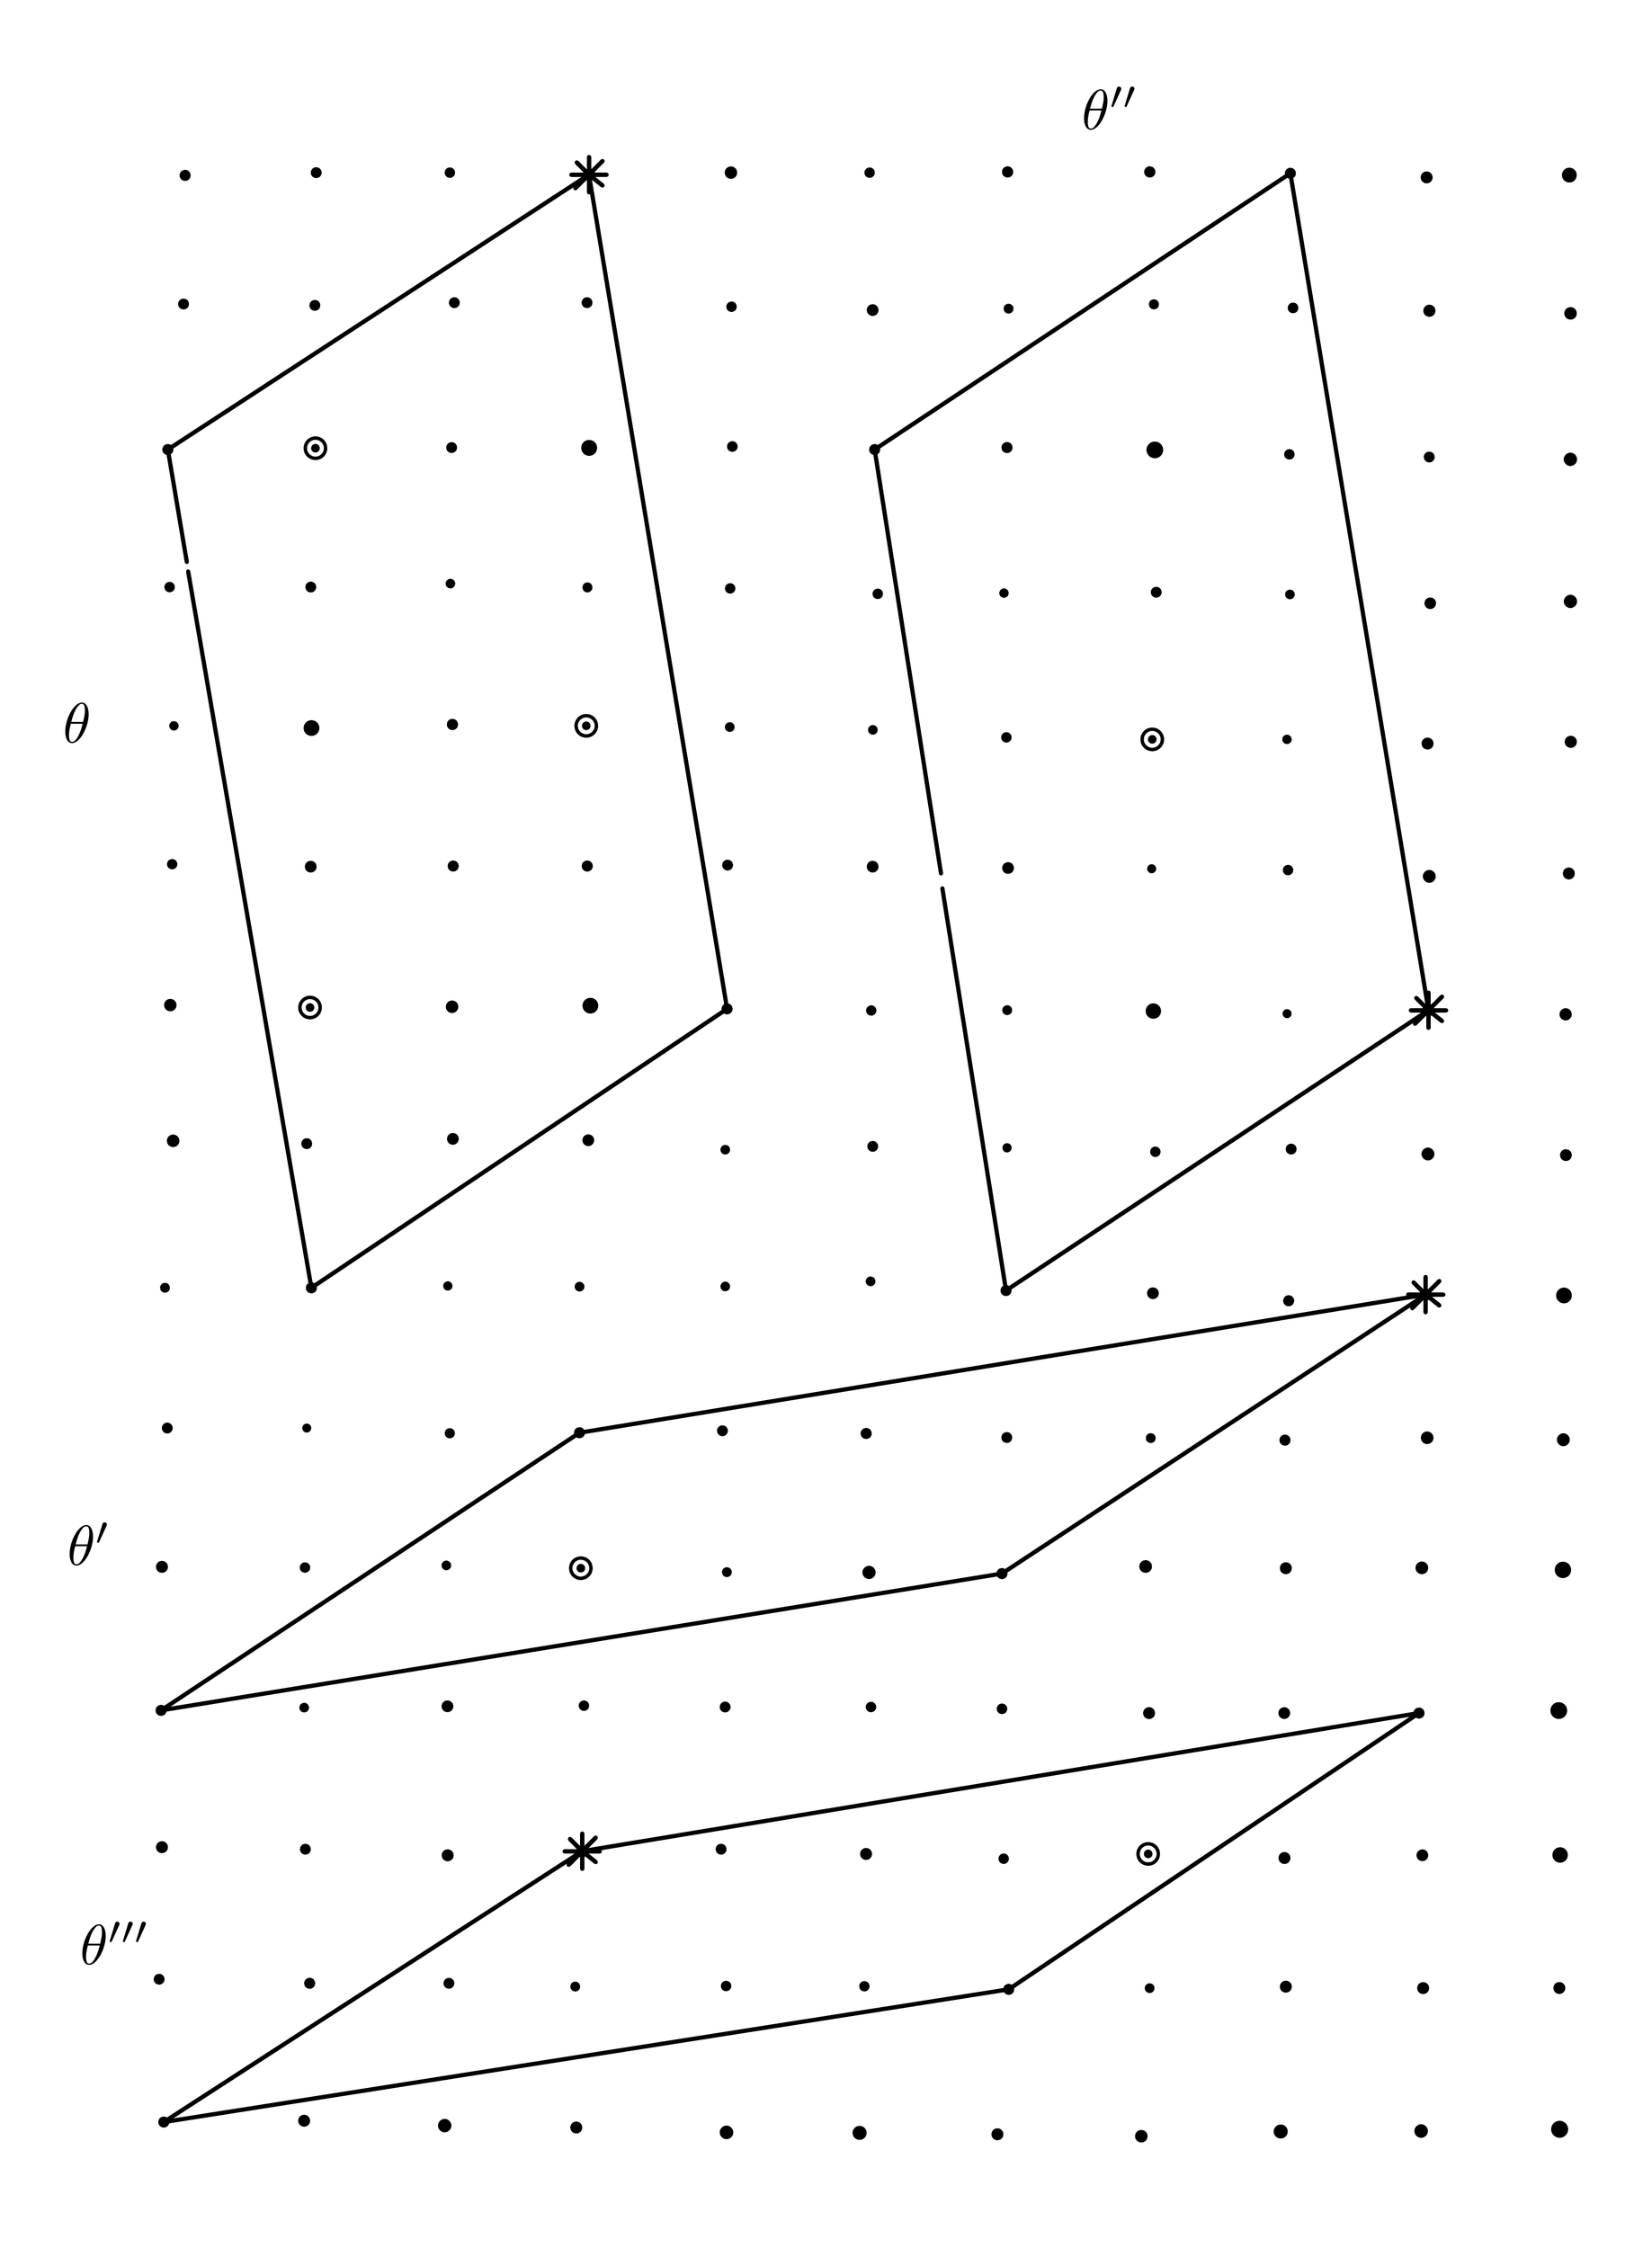
\begin{tikzpicture}[x=1bp,y=-1bp,line cap=round,line join=round]
\path[use as bounding box] (0,0) rectangle (1200,1640);
\begin{pgfinterruptboundingbox}
\draw[line width=3.1bp] (114,322) -- (425,119) -- (527,735) -- (220,941) -- (129,412);
\draw[line width=3.1bp] (128,405) -- (114,322);
\draw[line width=3.1bp] (636,322) -- (943,118) -- (1045,736) -- (733,943) -- (686,646);
\draw[line width=3.1bp] (685,635) -- (636,322);
\draw[line width=3.1bp] (109,1253) -- (418,1048) -- (1043,946) -- (730,1152) -- cycle;
\draw[line width=3.1bp] (111,1557) -- (420,1357) -- (1038,1255) -- (735,1459) -- cycle;
\fill (126.74,119.53) circle[radius=4.11bp];
\fill (223.57,117.53) circle[radius=4.03bp];
\fill (322.28,117.53) circle[radius=3.87bp];
\fill (425,119) circle[radius=4.5bp];
\draw[line width=3.2bp] (425,119) -- (425,106);
\draw[line width=3.2bp] (425,119) -- (435,109);
\draw[line width=3.2bp] (425,119) -- (438,119);
\draw[line width=3.2bp] (425,119) -- (435,127);
\draw[line width=3.2bp] (425,119) -- (425,132);
\draw[line width=3.2bp] (425,119) -- (415,129);
\draw[line width=3.2bp] (425,119) -- (412,119);
\draw[line width=3.2bp] (425,119) -- (416,110);
\fill (529.85,117.52) circle[radius=4.62bp];
\fill (632.28,117.53) circle[radius=3.87bp];
\fill (734.18,117.0) circle[radius=4.18bp];
\fill (839.18,117.0) circle[radius=4.18bp];
\fill (943,118) circle[radius=4.1bp];
\fill (1043.65,121.02) circle[radius=4.44bp];
\fill (1149.04,119.35) circle[radius=5.47bp];
\fill (125.57,214.53) circle[radius=4.03bp];
\fill (222.57,215.53) circle[radius=4.03bp];
\fill (325.57,213.53) circle[radius=4.03bp];
\fill (423.57,213.53) circle[radius=4.03bp];
\fill (530.28,216.53) circle[radius=3.87bp];
\fill (634.5,219.0) circle[radius=4.37bp];
\fill (734.88,217.95) circle[radius=3.66bp];
\fill (842.23,214.77) circle[radius=3.74bp];
\fill (944.98,217.41) circle[radius=3.95bp];
\fill (1045.66,219.5) circle[radius=4.51bp];
\fill (1149.91,221.44) circle[radius=4.65bp];
\fill (114,322) circle[radius=4.1bp];
\fill (223,321) circle[radius=3.2bp];
\draw[line width=2.5bp] (223,321) circle[radius=7.5bp];
\fill (323.57,320.53) circle[radius=4.03bp];
\fill (425.14,320.75) circle[radius=5.86bp];
\fill (530.88,319.73) circle[radius=3.95bp];
\fill (636,322) circle[radius=4.1bp];
\fill (733.74,320.53) circle[radius=4.11bp];
\fill (842.9,322.25) circle[radius=6.15bp];
\fill (942.28,325.53) circle[radius=3.87bp];
\fill (1045.57,327.53) circle[radius=4.03bp];
\fill (1149.8,329.21) circle[radius=4.92bp];
\fill (115.28,423.53) circle[radius=3.87bp];
\fill (219.57,423.53) circle[radius=4.03bp];
\fill (322.68,420.98) circle[radius=3.57bp];
\fill (423.88,423.79) circle[radius=3.7bp];
\fill (529.28,424.53) circle[radius=3.87bp];
\fill (638.28,428.53) circle[radius=3.87bp];
\fill (731.5,428.0) circle[radius=3.48bp];
\fill (843.94,427.35) circle[radius=4.03bp];
\fill (942.68,428.98) circle[radius=3.57bp];
\fill (1046.31,435.5) circle[radius=4.3bp];
\fill (1149.84,434.13) circle[radius=4.89bp];
\fill (118.5,526.0) circle[radius=3.48bp];
\fill (220.06,527.64) circle[radius=5.81bp];
\fill (324.18,525.0) circle[radius=4.18bp];
\fill (423,526) circle[radius=3.2bp];
\draw[line width=2.5bp] (423,526) circle[radius=7.5bp];
\fill (528.98,526.88) circle[radius=3.61bp];
\fill (634.67,528.98) circle[radius=3.57bp];
\fill (733.28,534.53) circle[radius=3.87bp];
\fill (841,536) circle[radius=3.2bp];
\draw[line width=2.5bp] (841,536) circle[radius=7.5bp];
\fill (940.5,536.0) circle[radius=3.48bp];
\fill (1044.31,539.1) circle[radius=4.44bp];
\fill (1150.09,537.81) circle[radius=4.51bp];
\fill (117.2,628.17) circle[radius=3.83bp];
\fill (219.5,630.0) circle[radius=4.37bp];
\fill (324.74,629.53) circle[radius=4.11bp];
\fill (423.74,629.53) circle[radius=4.11bp];
\fill (527.39,628.84) circle[radius=4.03bp];
\fill (634.5,630.0) circle[radius=4.37bp];
\fill (734.5,631.0) circle[radius=4.37bp];
\fill (840.57,631.54) circle[radius=3.34bp];
\fill (941.28,632.53) circle[radius=3.87bp];
\fill (1045.61,637.17) circle[radius=4.75bp];
\fill (1148.65,635.02) circle[radius=4.44bp];
\fill (115.82,732.21) circle[radius=4.62bp];
\fill (219,734) circle[radius=3.2bp];
\draw[line width=2.5bp] (219,734) circle[radius=7.5bp];
\fill (323.91,733.44) circle[radius=4.65bp];
\fill (426.06,732.64) circle[radius=5.81bp];
\fill (527,735) circle[radius=4.1bp];
\fill (633.46,736.2) circle[radius=3.83bp];
\fill (733.88,735.95) circle[radius=3.66bp];
\fill (841.81,736.62) circle[radius=5.67bp];
\fill (940.57,738.54) circle[radius=3.34bp];
\fill (1045,736) circle[radius=4.5bp];
\draw[line width=3.2bp] (1045,736) -- (1045,723);
\draw[line width=3.2bp] (1045,736) -- (1055,726);
\draw[line width=3.2bp] (1045,736) -- (1058,736);
\draw[line width=3.2bp] (1045,736) -- (1055,744);
\draw[line width=3.2bp] (1045,736) -- (1045,749);
\draw[line width=3.2bp] (1045,736) -- (1035,746);
\draw[line width=3.2bp] (1045,736) -- (1032,736);
\draw[line width=3.2bp] (1045,736) -- (1036,727);
\fill (1146.29,739.03) circle[radius=4.55bp];
\fill (117.91,832.44) circle[radius=4.65bp];
\fill (216.57,834.53) circle[radius=4.03bp];
\fill (324.5,831.0) circle[radius=4.37bp];
\fill (424.5,832.0) circle[radius=4.37bp];
\fill (525.67,838.98) circle[radius=3.57bp];
\fill (634.57,836.53) circle[radius=4.03bp];
\fill (733.76,837.59) circle[radius=3.43bp];
\fill (843.28,840.53) circle[radius=3.87bp];
\fill (943.57,838.53) circle[radius=4.03bp];
\fill (1044.61,842.17) circle[radius=4.75bp];
\fill (1146.5,843.0) circle[radius=4.37bp];
\fill (111.88,940.95) circle[radius=3.66bp];
\fill (220,941) circle[radius=4.1bp];
\fill (320.76,939.59) circle[radius=3.43bp];
\fill (418.05,940.12) circle[radius=3.61bp];
\fill (525.67,939.98) circle[radius=3.57bp];
\fill (632.98,936.2) circle[radius=3.61bp];
\fill (733,943) circle[radius=4.1bp];
\fill (841.5,945.0) circle[radius=4.37bp];
\fill (941.74,950.53) circle[radius=4.11bp];
\fill (1043,946) circle[radius=4.5bp];
\draw[line width=3.2bp] (1043,946) -- (1043,933);
\draw[line width=3.2bp] (1043,946) -- (1053,936);
\draw[line width=3.2bp] (1043,946) -- (1056,946);
\draw[line width=3.2bp] (1043,946) -- (1053,954);
\draw[line width=3.2bp] (1043,946) -- (1043,959);
\draw[line width=3.2bp] (1043,946) -- (1033,956);
\draw[line width=3.2bp] (1043,946) -- (1030,946);
\draw[line width=3.2bp] (1043,946) -- (1034,937);
\fill (1145.06,946.64) circle[radius=5.81bp];
\fill (113.57,1044.53) circle[radius=4.03bp];
\fill (216.57,1044.54) circle[radius=3.34bp];
\fill (322.22,1048.38) circle[radius=3.78bp];
\fill (418,1048) circle[radius=4.1bp];
\fill (523.57,1046.53) circle[radius=4.03bp];
\fill (629.74,1048.53) circle[radius=4.11bp];
\fill (733.57,1051.53) circle[radius=4.03bp];
\fill (839.88,1051.95) circle[radius=3.66bp];
\fill (939.02,1053.45) circle[radius=4.11bp];
\fill (1044.03,1051.71) circle[radius=4.69bp];
\fill (1144.61,1053.17) circle[radius=4.75bp];
\fill (109.65,1147.02) circle[radius=4.44bp];
\fill (215.28,1147.53) circle[radius=3.87bp];
\fill (319.68,1145.97) circle[radius=3.57bp];
\fill (419,1148) circle[radius=3.2bp];
\draw[line width=2.5bp] (419,1148) circle[radius=7.5bp];
\fill (526.88,1150.95) circle[radius=3.66bp];
\fill (631.84,1151.13) circle[radius=4.89bp];
\fill (730,1152) circle[radius=4.1bp];
\fill (836.11,1146.76) circle[radius=4.72bp];
\fill (939.65,1148.02) circle[radius=4.44bp];
\fill (1040.11,1147.76) circle[radius=4.72bp];
\fill (1144.3,1149.26) circle[radius=6.05bp];
\fill (109,1253) circle[radius=4.1bp];
\fill (214.68,1250.97) circle[radius=3.57bp];
\fill (320.5,1250.0) circle[radius=4.37bp];
\fill (421.28,1249.53) circle[radius=3.87bp];
\fill (525.57,1250.53) circle[radius=4.03bp];
\fill (633.28,1250.53) circle[radius=3.87bp];
\fill (730.02,1251.85) circle[radius=3.91bp];
\fill (838.65,1255.02) circle[radius=4.44bp];
\fill (938.5,1255.0) circle[radius=4.37bp];
\fill (1038,1255) circle[radius=4.1bp];
\fill (1141.22,1253.14) circle[radius=6.18bp];
\fill (109.65,1354.02) circle[radius=4.44bp];
\fill (215.57,1355.53) circle[radius=4.03bp];
\fill (320.65,1360.02) circle[radius=4.44bp];
\fill (420,1357) circle[radius=4.5bp];
\draw[line width=3.2bp] (420,1357) -- (420,1344);
\draw[line width=3.2bp] (420,1357) -- (430,1347);
\draw[line width=3.2bp] (420,1357) -- (433,1357);
\draw[line width=3.2bp] (420,1357) -- (430,1365);
\draw[line width=3.2bp] (420,1357) -- (420,1370);
\draw[line width=3.2bp] (420,1357) -- (410,1367);
\draw[line width=3.2bp] (420,1357) -- (407,1357);
\draw[line width=3.2bp] (420,1357) -- (411,1348);
\fill (522.57,1355.53) circle[radius=4.03bp];
\fill (629.65,1359.02) circle[radius=4.44bp];
\fill (731.28,1362.53) circle[radius=3.87bp];
\fill (838,1359) circle[radius=3.2bp];
\draw[line width=2.5bp] (838,1359) circle[radius=7.5bp];
\fill (938.65,1362.02) circle[radius=4.44bp];
\fill (1040.5,1360.0) circle[radius=4.37bp];
\fill (1142.22,1359.78) circle[radius=5.7bp];
\fill (107.57,1451.53) circle[radius=4.03bp];
\fill (218.74,1454.53) circle[radius=4.11bp];
\fill (321.57,1454.53) circle[radius=4.03bp];
\fill (414.88,1456.95) circle[radius=3.66bp];
\fill (526.28,1456.53) circle[radius=3.87bp];
\fill (628.41,1456.72) circle[radius=3.83bp];
\fill (735,1459) circle[radius=4.1bp];
\fill (839.05,1458.12) circle[radius=3.61bp];
\fill (939.65,1457.02) circle[radius=4.44bp];
\fill (1041.06,1458.08) circle[radius=4.44bp];
\fill (1141.65,1458.02) circle[radius=4.44bp];
\fill (111,1557) circle[radius=4.1bp];
\fill (214.65,1556.02) circle[radius=4.44bp];
\fill (318.44,1559.62) circle[radius=4.95bp];
\fill (415.65,1561.02) circle[radius=4.44bp];
\fill (526.58,1564.62) circle[radius=5.01bp];
\fill (624.87,1564.98) circle[radius=5.17bp];
\fill (726.65,1566.02) circle[radius=4.44bp];
\fill (832.91,1567.44) circle[radius=4.65bp];
\fill (935.87,1563.98) circle[radius=5.17bp];
\fill (1039.58,1563.62) circle[radius=5.01bp];
\fill (1141.86,1562.33) circle[radius=6.26bp];
\node[inner sep=0pt,outer sep=0pt,anchor=center] at (47,524) {\scalebox{4.2}{\ensuremath{\theta}}};
\node[inner sep=0pt,outer sep=0pt,anchor=center] at (56,1130) {\scalebox{4.2}{\ensuremath{\theta'}}};
\node[inner sep=0pt,outer sep=0pt,anchor=center] at (810,70) {\scalebox{4.2}{\ensuremath{\theta''}}};
\node[inner sep=0pt,outer sep=0pt,anchor=center] at (75,1425) {\scalebox{4.2}{\ensuremath{\theta'''}}};
\end{pgfinterruptboundingbox}
\end{tikzpicture}
}
\end{center}

\SourceLeaf{370}%
% A544-P0370-D01
\Article{13}
Hieraus fliesst folgende Regel. Es sei das Resultat aus den Vorschriften
\[
\mathrm{II}\pdot\pdot\pdot\;G,\quad
\mathrm{III}\pdot\pdot\pdot\;g,\quad
\mathrm{IV}\pdot\pdot\pdot\;H,\quad
\mathrm{V}\pdot\pdot\pdot\;h
\]
So ist
\[
\begin{aligned}
4\Theta&=R=0\\
4\Theta'&=-g+G-h-H+R'\\
4\Theta''&=-2g+2G+R''\\
4\Theta'''&=-g+G+h+H+R'''
\end{aligned}
\]

% A544-P0370-D02
In unserm Beispiele ist
\[
\begin{gathered}
G=0,\quad g=-1,\quad H=-1,\quad h=+2,\\
R'=0,\quad R''=+2,\quad R'''=-2\\
4\Theta=0,\quad4\Theta'=+1-1+0=0,\\
4\Theta''=+2+2=+4,\quad4\Theta'''=+1+1-2=0
\end{gathered}
\]
und die Correctionen $R,R'$ etc. werden so bestimmt: Es ist

% A544-P0370-D03
\[
R=\left\{\begin{array}{l}
-(\beta)+\frac12(\alpha\beta)+\frac12(\alpha\beta abAB)\\
-\frac12(b)-\frac12(B)\\
+(\beta)-\frac12(\alpha\beta)-\frac12(\alpha\beta abAB)\\
+\frac12(b)+\frac12(B)
\end{array}\right.
\]

% A544-P0370-D04
\[
R'=\left\{\begin{array}{l}
+(\alpha)-\frac12(\alpha\beta)+\frac12(\alpha\beta abAB)\\
-\frac12(b)-\frac12(A)\\
0\\
-\frac12(a)+\frac12(B)
\end{array}\right.
\]

% A544-P0370-D05
\[
R''=\left\{\begin{array}{l}
+(\beta)+\frac12(\alpha\beta)+\frac12(\alpha\beta abAB)\\
-\frac12(b)+\frac12(B)\\
+(\beta)+\frac12(\alpha\beta)+\frac12(\alpha\beta abAB)\\
-\frac12(b)+\frac12(B)
\end{array}\right.
\]

% A544-P0370-D06
\[
R'''=\left\{\begin{array}{l}
-(\alpha)-\frac12(\alpha\beta)+\frac12(\alpha\beta abAB)\\
-\frac12(b)+\frac12(A)\\
0\\
+\frac12(a)+\frac12(B)
\end{array}\right.
\]
wo die in Parenthese stehenden Grössen blos die Zeichen hergeben.


\SourceLeaf{371}%
% A544-P0371-D01
Es ist also
\[
R+R'+R''+R'''=2(\alpha\beta abAB)-2(b)+2(B)+2(\beta)
\]
folglich
\[
\begin{aligned}
\Theta+\Theta'+\Theta''+\Theta'''={}&-g+G+\tfrac12(\alpha\beta abAB)\\
&+\tfrac12(\beta)-\tfrac12(b)+\tfrac12(B)\\
={}&-g+G+S
\end{aligned}
\]

% A544-P0371-D02
\begingroup\small\setlength{\arraycolsep}{2.6pt}
\[
\begin{array}{ccccc||ccc||ccc||ccc}
\multicolumn{2}{c}{ab}&\multicolumn{3}{c||}{+\quad+}&\multicolumn{3}{c||}{-\quad+}&\multicolumn{3}{c||}{-\quad-}&\multicolumn{3}{c}{+\quad-}\\\hline
A&B&\alpha&\beta&S&\alpha&\beta&S&\alpha&\beta&S&\alpha&\beta&S\\
+&+&+&+&+1&-&+&+1&-&-&+1&+&-&+1\\
&&+&-&-1&+&+&0&-&+&+1&-&-&0\\
-&+&+&-&0&+&+&+1&-&+&+2&-&-&+1\\
&&-&-&-1&+&-&-1&+&+&+1&-&+&+1\\
-&-&-&-&-1&+&-&-1&+&+&+1&-&+&+1\\
&&-&+&-1&-&-&-2&+&-&-1&+&+&0\\
+&-&-&+&0&-&-&-1&+&-&0&+&+&+1\\
&&+&+&-1&-&+&-1&-&-&-1&+&-&-1\\
\end{array}
\]
\endgroup

% A544-P0371-D03
\Article{14}
Hienach bekommt nun die erste Regel folgende Gestalt:
\[
\begin{aligned}
4\,\text{Dec.}={}&\text{I.}\;-4\Sigma\varepsilon\ \text{von denen, wo }y\text{ ganz, }[x]\text{ gerade}\\
&\text{II.}\;+4\Sigma\varepsilon\ \text{von denen, wo }[x]\text{ gerade, }[y]\text{ ungerade}\\
&\text{III.}\;-\Sigma\varepsilon\ \text{von allen}\\
&\text{IV.}\;+4\Sigma\varepsilon\ \text{von denen, wo nicht zugleich}\\
&\qquad [x]\text{ und }[y]\text{ gerade}\\
&+Q+S
\end{aligned}
\]

% A544-P0371-D04
In unserm Beispiel
\[
\begin{array}{rc}
\mathrm{I}\dotsfour&0\\
\mathrm{II}\dotsfour&-4\\
\mathrm{III}&+1\\
\mathrm{IV}&0\\
Q&-5\\
S&0\\\cline{2-2}
&-8
\end{array}
\]
Man denke sich nun in III diejenigen besonders bemerkt, wo $y$ ganz, $[x]$ gerade, so ist

\SourceLeaf{372}%
% A544-P0372-D01
\[
\begin{gathered}
\left.\begin{array}{rl}
\mathrm{III.}&\Sigma\varepsilon\ \text{von allen}\\
&-4\Sigma\varepsilon\ \text{der besonderen}
\end{array}\right\}\\
={}\text{Intensor }(\tfrac12-\omega)m-\text{Intens. }\omega m=-W
\end{gathered}
\]
Hier ist
\[
W=\begin{array}{cc|rr}
a&b&&\\
+&+&-3&-1\\
-&+&-2&0\\
-&-&+2&0\\
-&+&+3&+1\\[3pt]
&&\frac{m-1}{2}&\frac{m-1}{2}\\
&&\text{par}&\text{impar}
\end{array}
\]

% A544-P0372-D02
Also
\[
\begin{aligned}
4\,\text{Decident}={}&\text{I.}\;-4\Sigma\varepsilon\quad y\text{ ganz, }[x]\text{ gerade}\\
&\text{II.}\;+4\Sigma\varepsilon\quad[x]\text{ gerade, }[y]\text{ ungerade}\\
&\text{III.}\;-4\Sigma\varepsilon\quad y\text{ ganz, }[x]\text{ gerade}\\
&\text{IV.}\;+4\Sigma\varepsilon\quad\text{alle wo nicht zugleich }[x],[y]\text{ gerade}\\
&+Q+S+W
\end{aligned}
\]

% A544-P0372-D03
\begin{center}Tabelle für $\frac14(Q+S+W)$\end{center}
\begingroup\small\setlength{\arraycolsep}{2pt}
\[
\begin{array}{cccccc|rr||cccccc|rr}
a&b&A&B&\alpha&\beta&&&a&b&A&B&\alpha&\beta&&\\
+&+&+&+&+&+&0&0&-&-&+&+&-&-&0&0\\
&&&&+&-&-1&0&&&&&-&+&+1&0\\
&&-&+&+&-&-1&-1&&&-&+&-&+&0&-1\\
&&&&-&-&-1&-1&&&&&+&+&0&-1\\
&&-&-&-&-&-2&-1&&&-&-&+&+&0&-1\\
&&&&-&+&-1&-1&&&&&+&-&-1&-1\\
&&+&-&-&+&-1&0&&&+&-&+&-&0&0\\
&&&&+&+&-1&0&&&&&-&-&0&0\\[3pt]
-&+&+&+&-&+&0&0&+&-&+&+&+&-&+1&+1\\
&&&&+&+&0&0&&&&&-&-&0&0\\
&&-&+&+&+&-1&-1&&&-&+&-&-&+1&0\\
&&&&+&-&-1&-1&&&&&-&+&0&-1\\
&&-&-&+&-&-2&-1&&&-&-&-&+&+1&0\\
&&&&-&-&-2&-1&&&&&+&+&0&-1\\
&&+&-&-&-&-1&0&&&+&-&+&+&+1&+1\\
&&&&-&+&-1&0&&&&&+&-&0&0\\
\end{array}
\]
\endgroup

\SourceLeaf{373}%
% A544-P0373-D01
\Article{15}
Die zweite Methode ist folgende:
\[
\begin{aligned}
\text{Decident}={}&\text{I.}\;+\Sigma\varepsilon,\ \text{wo }Y\text{ ganz, }[X]\text{ gerade}\\
&-4\Sigma\varepsilon,\ \text{unter diesen, wo noch }y\text{ ganz, }[x]\text{ gerade}\\
&\text{II.}\;+\Sigma\lambda\varepsilon,\ \text{wo }Y\text{ ganz, }[X]\text{ gerade;}\\
&\qquad\lambda\text{ ist der Intensor von }p\\
&\text{II.}\;-\Sigma\lambda'\varepsilon,\ \text{wo }X\text{ ganz, }[Y]\text{ ungerade}\\
&\qquad\lambda'\text{ der Intensor von }ip=1,\,2,\,3,\,0\\
&\qquad\qquad\text{wenn }\lambda=0,\,1,\,2,\,3\\
&\text{IV.}\;+\Sigma\lambda\varepsilon,\ \text{wo }Y\text{ ganz, }[X]\text{ gerade,}\\
&\qquad\lambda\text{ der Intensor von }p\\
&\text{IV.}\;+\Sigma\lambda'\varepsilon,\ \text{wo }X\text{ ganz, }[Y]\text{ gerade}\\
&\qquad\lambda'\text{ der Intensor von }im-ip=0\quad3\quad2\quad1\\
&\qquad\qquad\text{wenn Int. }p=0\quad1\quad2\quad3\\
&+q
\end{aligned}
\]

% A544-P0373-D02
Hier ist $q=0$, wenn $\frac{M-1}{2}$ ungerade i.\,e. nur durch $1+i$, nicht durch $2$ theilbar, und nicht zugleich $AB\,+\,-$, hingegen übrigens
\begingroup\small\setlength{\arraycolsep}{2pt}
\[
\begin{array}{cc|l||rr|rr|rr|rr}
&&&\alpha&\beta&\alpha&\beta&\alpha&\beta&\alpha&\beta\\
A&B&&+&+&-&+&-&-&+&-\\
+&+&\text{Int. }\frac12(m-\omega\mu)&+3&+1&+3&+1&+0&+2&+0&+2\\
-&+&0&\multicolumn{2}{c|}{0}&\multicolumn{2}{c|}{0}&\multicolumn{2}{c|}{0}&\multicolumn{2}{c}{0}\\
-&-&-\text{Int. }\frac12(m+\omega\mu)&-0&-2&-0&-2&-3&-1&-3&-1\\
+&-&-\text{Int. }\omega\mu&\multicolumn{2}{c|}{-0}&\multicolumn{2}{c|}{-1}&\multicolumn{2}{c|}{-2}&\multicolumn{2}{c}{-3}
\end{array}
\]
\endgroup
wo doppelte Zahlen stehen, gilt die erste für gerade $\frac{m-1}{2}$, die andere für ungerade.

% A544-P0373-D03
In unserm Beispiele:
\[
\begin{array}{rc|r|r|r|r}
\mathrm{I.}&y&Y&20x&20Y&\varepsilon\\
&0&-1&+13&+9&+1^{*}\\
&0&-2&+26&+18&+1\\
&+1&-1&+22&+46&+1\\
&&&&&+3(+1)
\end{array}
\qquad
\begin{array}{r}
+3\\-4\\-1\\\hline
\text{Dec.}=-2
\end{array}
\]

% A544-P0373-D04
II. desunt.
\begingroup\small\setlength{\arraycolsep}{2pt}
\[
\begin{array}{rc|r|r|r|r|r|r|r}
\mathrm{IV.}&X&12x&12y&12Y&\varepsilon&\lambda&\lambda'&\lambda'\varepsilon\\
&0&+20+20\omega&-9&-37&-1&2&2&-2\\
&+1&+24+20\omega&-3&-39&+1&3&1&+1\\
&+2&+28+20\omega&+3&-41&-1&0&0&0\\
&&&&&&&&-1
\end{array}
\]
\endgroup

\SourceLeaf{374}%
% A544-P0374-D01
Was aus II genommen ist, vereinigt sich in folgendes Resultat
\[
\begin{aligned}
\mathrm{II.}\;&-\Sigma\varepsilon,\ \text{wo }Y\text{ ganz, }[X]\text{ gerade}\\
&+4\Sigma\varepsilon,\ \text{von eben diesen, wenn zugleich }[x]\text{ gerade,}\\
&\qquad[y]\text{ ungerade}\\
\mathrm{II.}\;&+\Sigma\lambda'\varepsilon,\ \text{wo }Y\text{ ganz, }[X]\text{ gerade}\\
&-\Sigma\lambda'\varepsilon,\ \text{wo }X\text{ ganz, }[Y]\text{ ungerade,}\\
&\qquad\lambda'\text{ der Intensor von }ip
\end{aligned}
\]

% A544-P0374-D02
Die beiden letzten Theile vereinigen sich wiederum in
\[
\begin{aligned}
\mathrm{III.}\;&+\Sigma\varepsilon,\ \text{wo }[X]\text{ gerade, }[Y]\text{ ungerade}\\
&-4\Sigma\varepsilon,\ \text{wenn zugleich }x\text{ eine Ganze, }[y]\text{ ungerade}\\
&+r+s
\end{aligned}
\]
wo $r=0$, wenn $AB\dotsfive\left\{\begin{array}{cc}+&+\\-&+\\-&-\end{array}\right.$

% A544-P0374-D03
und $r=\text{Int. }\omega mi$, wenn $AB\dotstwo+\,-$
\[
\begin{gathered}
s=-\text{Int. }(\tfrac12-\omega)mi,\quad\text{wenn }\frac{M-1}{2}\text{ gerade und }B\text{ positiv,}\\
\text{in allen andern Fällen }=0
\end{gathered}
\]

% A544-P0374-D04
In unserm Beispiele
\[
\text{III. Fällt aus.}\quad r=0,\ s=0
\]
Was aus IV genommen ist, vereinigt sich in folgendes Resultate
\[
\begin{aligned}
\mathrm{IV.}\;&+4\Sigma\varepsilon,\ \text{wo }Y\text{ ganz, }[X]\text{ gerade und nicht zugleich}\\
&\qquad[x]\text{ gerade, }[y]\text{ gerade}\\
&-\Sigma\lambda'\varepsilon,\ \text{wo }Y\text{ ganz, }[X]\text{ gerade}\\
&+\Sigma\lambda'\varepsilon,\ \text{wo }X\text{ ganz, }[Y]\text{ gerade}\\
&\qquad\text{wo }\lambda'\text{ Int. von }im-ip
\end{aligned}
\]

% A544-P0374-D05
Die zwei letzten Theile vereinigen sich wiederum zu
\[
\begin{aligned}
\mathrm{V.}\;&+\Sigma\varepsilon,\ \text{wo nicht zugleich }[X]\text{ und }[Y]\text{ gerade}\\
&-4\Sigma\varepsilon,\ \text{wo zugleich }x\text{ eine Ganze, }[y]\text{ gerade}\\
&+w
\end{aligned}
\]
Hier ist $w=0$, wenn $\frac{M-1}{2}$ gerade und $A$ positiv; in allen übrigen Fällen
\[
=-\text{Intensor }(\tfrac12i+\omega)m
\]

\SourceLeaf{375}%
% A544-P0375-D01
In unserm Beispiele
\[
\begin{gathered}
\mathrm{V.}\\
\begin{array}{c|r|r|r|r}
y&6x&6X&6Y&\varepsilon\\
0&+13&+9&-20&+1
\end{array}\\
w=-2
\end{gathered}
\]

% A544-P0375-D02
\begin{center}Tafel für $q,r,s,w$ und deren Summe.\end{center}
\begingroup\scriptsize\setlength{\arraycolsep}{1.1pt}\renewcommand{\arraystretch}{1.12}
\[
\begin{array}{cccccc|rrrrr|rrrrr|rrrrr|rrrrr}
a&b&A&B&\alpha&\beta&\multicolumn{5}{c|}{\begin{array}{c}\frac{M-1}{2}\ \text{ger.}\\\frac{m-1}{2}\ \text{ger.}\end{array}}&\multicolumn{5}{c|}{\begin{array}{c}\frac{M-1}{2}\ \text{ung.}\\\frac{m-1}{2}\ \text{ger.}\end{array}}&\multicolumn{5}{c|}{\begin{array}{c}\frac{M-1}{2}\ \text{ger.}\\\frac{m-1}{2}\ \text{ung.}\end{array}}&\multicolumn{5}{c|}{\begin{array}{c}\frac{M-1}{2}\ \text{ung.}\\\frac{m-1}{2}\ \text{ung.}\end{array}}\\[4pt]
+&+&+&+&+&+&+3&0&0&0&+3&0&0&0&0&0&+1&0&-2&0&-1&0&0&0&-2&-2\\
&&&&+&-&0&0&0&0&0&0&0&0&0&0&+2&0&-2&0&0&0&0&0&-2&-2\\
&&-&+&+&-&0&0&0&0&0&0&0&0&0&0&0&0&-2&-2&-4&0&0&0&-2&-2\\
&&&&-&-&0&0&0&0&0&0&0&0&0&0&0&0&-2&-2&-4&0&0&0&-2&-2\\
&&-&-&-&-&-3&0&0&0&-3&0&0&0&0&0&-1&0&0&-2&-3&0&0&0&-2&-2\\
&&&&-&+&0&0&0&0&0&0&0&0&0&0&-2&0&0&-2&-4&0&0&0&-2&-2\\
&&+&-&-&+&-1&+1&0&0&0&-1&+1&0&0&0&-1&+1&0&0&0&-1&+1&0&-2&-2\\
&&&&+&+&0&+1&0&0&+1&0&+1&0&0&+1&0&+1&0&0&+1&0&+1&0&-2&-1\\[4pt]
-&+&+&+&-&+&+3&0&0&0&+3&0&0&0&-1&-1&+1&0&-2&0&-1&0&0&0&-3&-3\\
&&&&+&+&+3&0&0&0&+3&0&0&0&-1&-1&+1&0&-2&0&-1&0&0&0&-3&-3\\
&&-&+&+&+&0&0&0&-1&-1&0&0&0&-1&-1&0&0&-2&-3&-5&0&0&0&-3&-3\\
&&&&+&-&0&0&0&-1&-1&0&0&0&-1&-1&0&0&-2&-3&-5&0&0&0&-3&-3\\
&&-&-&+&-&-3&0&0&-1&-4&0&0&0&-1&-1&-1&0&0&-3&-4&0&0&0&-3&-3\\
&&&&-&-&-3&0&0&-1&-4&0&0&0&-1&-1&-1&0&0&-3&-4&0&0&0&-3&-3\\
&&+&-&-&-&-2&+2&0&0&0&-2&+2&0&-1&-1&-2&+2&0&0&0&-2&+2&0&-3&-3\\
&&&&-&+&-1&+2&0&0&+1&-1&+2&0&-1&0&-1&+2&0&0&+1&-1&+2&0&-3&-2\\[4pt]
-&-&+&+&-&-&0&0&-1&0&-1&0&0&0&-1&-1&+2&0&-3&0&-1&0&0&0&-3&-3\\
&&&&-&+&+3&0&-1&0&+2&0&0&0&-1&-1&+1&0&-3&0&-2&0&0&0&-3&-3\\
&&-&+&-&+&0&0&-1&-1&-2&0&0&0&-1&-1&0&0&-3&-3&-6&0&0&0&-3&-3\\
&&&&+&+&0&0&-1&-1&-2&0&0&0&-1&-1&0&0&-3&-3&-6&0&0&0&-3&-3\\
&&-&-&+&+&0&0&0&-1&-1&0&0&0&-1&-1&-2&0&0&-3&-5&0&0&0&-3&-3\\
&&&&+&-&-3&0&0&-1&-4&0&0&0&-1&-1&-1&0&0&-3&-4&0&0&0&-3&-3\\
&&+&-&+&-&-3&+3&0&0&0&-3&+3&0&-1&-1&-3&+3&0&0&0&-3&+3&0&-3&-3\\
&&&&-&-&-2&+3&0&0&+1&-2&+3&0&-1&0&-2&+3&0&0&+1&-2&+3&0&-3&-2\\[4pt]
+&-&+&+&+&-&0&0&-1&0&-1&0&0&0&0&0&+2&0&-3&0&-1&0&0&0&-2&-2\\
&&&&-&-&0&0&-1&0&-1&0&0&0&0&0&+2&0&-3&0&-1&0&0&0&-2&-2\\
&&-&+&-&-&0&0&-1&0&-1&0&0&0&0&0&0&0&-3&-2&-5&0&0&0&-2&-2\\
&&&&-&+&0&0&-1&0&-1&0&0&0&0&0&0&0&-3&-2&-5&0&0&0&-2&-2\\
&&-&-&-&+&0&0&0&0&0&0&0&0&0&0&-2&0&0&-2&-4&0&0&0&-2&-2\\
&&&&+&+&0&0&0&0&0&0&0&0&0&0&-2&0&0&-2&-4&0&0&0&-2&-2\\
&&+&-&+&+&0&0&0&0&0&0&0&0&0&0&0&0&0&0&0&0&0&0&-2&-2\\
&&&&+&-&-3&0&0&0&-3&-3&0&0&0&-3&-3&0&0&0&-3&-3&0&0&-2&-5\\
\end{array}
\]
\endgroup


\SourceLeaf{376}%
% A544-P0376-D01
\Article{16}
Es ist folglich
\[
\text{Dec. }\frac mM-\text{Dec. }\frac Mm=
\]
\[
\begin{aligned}
\mathrm{I.}\;&-4\Sigma\varepsilon,\ \text{wo }y,Y\text{ ganz, }[x],[X]\text{ gerade}\\
\mathrm{II.}\;&+4\Sigma\varepsilon,\ Y\text{ ganz, }[X]\text{ gerade, }[x]\text{ gerade, }[y]\text{ ungerade}\\
\mathrm{III.}\;&-4\Sigma\varepsilon,\ x\text{ ganz, }[X]\text{ gerade, }[Y]\text{ ungerade,}\\
&\qquad [y]\text{ ungerade}\\
\mathrm{IV.}\;&+4\Sigma\varepsilon,\ Y\text{ ganz, }[X]\text{ gerade, und nicht zugleich }[x],[y]\text{ gerade}\\
\mathrm{V.}\;&-4\Sigma\varepsilon,\ x\text{ ganz, }[y]\text{ gerade und nicht zugleich }[X],[Y]\text{ gerade}\\
&+\psi
\end{aligned}
\]

% A544-P0376-D02
Hier ist $\psi$ in folgender Tabelle dargestellt
\begingroup\small\setlength{\arraycolsep}{1.8pt}
\[
\begin{array}{cccccc|rrrr||cccccc|rrrr}
a&b&A&B&\alpha&\beta&\multicolumn{4}{c||}{\psi}&a&b&A&B&\alpha&\beta&\multicolumn{4}{c}{\psi}\\
+&+&+&+&+&+&+4&0&0&-2&-&-&+&+&-&-&0&0&0&-2\\
&&+&+&+&-&0&0&0&-2&&&+&+&-&+&+4&0&0&-2\\
&&-&+&+&-&0&-4&0&-2&&&-&+&-&+&0&-4&0&-2\\
&&-&+&-&-&0&-4&0&-2&&&-&+&+&+&0&-4&0&-2\\
&&-&-&-&-&-4&-4&0&-2&&&-&-&+&+&0&-4&0&-2\\
&&-&-&-&+&0&-4&0&-2&&&-&-&+&-&-4&-4&0&-2\\
&&+&-&-&+&0&0&0&-2&&&+&-&+&-&0&0&0&-2\\
&&+&-&+&+&0&0&0&-2&&&+&-&-&-&0&0&0&-2\\[4pt]
-&+&+&+&-&+&+4&0&0&-2&+&-&+&+&+&-&0&0&0&-2\\
&&+&+&+&+&+4&0&0&-2&&&+&+&-&-&0&0&0&-2\\
&&-&+&+&+&0&-4&0&-2&&&-&+&-&-&0&-4&0&-2\\
&&-&+&+&-&0&-4&0&-2&&&-&+&-&+&0&-4&0&-2\\
&&-&-&+&-&-4&-4&0&-2&&&-&-&-&+&0&-4&0&-2\\
&&-&-&-&-&-4&-4&0&-2&&&-&-&+&+&0&-4&0&-2\\
&&+&-&-&-&0&0&0&-2&&&+&-&+&+&0&0&0&-2\\
&&+&-&-&+&0&0&0&-2&&&+&-&+&-&-4&-4&-4&-6\\
\end{array}
\]
\endgroup

% A544-P0376-D03
\[
\begin{array}{lll}
\text{Hier gelten die ersten beiden Columnen}&\text{für }\frac12(M-1)\text{ gerade}\\
\text{letzten beiden}&\text{für }\frac12(M-1)\text{ ungerade}\\
\text{die erste und dritte}&\text{für }\frac12(m-1)\text{ gerade}\\
\text{zweite und vierte}&\text{für }\frac12(m-1)\text{ ungerade}
\end{array}
\]

\SourceLeaf{377}%
% A544-P0377-D01
\Article{17}
Die $128$ Fälle, welche in obiger Tafel bei der Bestimmung von $\psi$ unterschieden sind, lassen sich viel kürzer auf folgende Weise umfassen:
\[
\psi=k+l
\]
$k=-4$, wenn zugleich $a,A,\alpha,b,B,\beta$ die Zeichen $+\ +\ +\ -\ -\ -$ haben, sonst immer
\[
k=0
\]

% A544-P0377-D02
\begingroup\small\setlength{\arraycolsep}{3pt}
\[
\begin{array}{ll|ll}
\frac12(M-1)\text{ gerade}&\frac12(m-1)\text{ gerade}&l=+4,&\text{wenn }AB\beta\text{ positiv}\\
&&-4,&\text{wenn }AB\beta\text{ negativ}\\
&&0,&\text{in allen übrigen Fällen}\\[3pt]
\frac12(M-1)\text{ gerade}&\frac12(m-1)\text{ ungerade}&l=-4,&\text{wenn }A\text{ negativ}\\
&&0,&\text{wenn }A\text{ positiv}\\[3pt]
\frac12(M-1)\text{ ungerade}&\frac12(m-1)\text{ gerade}&l=0&\\[3pt]
\frac12(M-1)\text{ ungerade}&\frac12(m-1)\text{ ungerade}&l=-2&
\end{array}
\]
\endgroup

% A544-P0377-D03
Zu versuchen ist noch, ob es vortheilhafter ist, $A$ und $a$ positiv, dagegen aber $m\equiv1$, $M\equiv1$ nur nach mod.\ $2$ (nicht nach Modulus $2+2i$) zu nehmen. Das Endresultat muss werden
\[
\text{Dec. }\frac mM-\text{Dec. }\frac Mm\equiv
\]
\[
\begin{array}{r|rrrr}
&\multicolumn{4}{c}{M\equiv}\\
m\equiv&1&1+2i&3&3+2i\\\hline
1&0&0&0&0\\
1+2i&0&2&2&0\\
3&0&2&0&2\\
3+2i&0&0&2&2
\end{array}
\]
Alles nach Mod.\ $4$.
\BookRule{.3\textwidth}

\SourceLeaf{378}%
% A544-P0378-D01
\par\bigskip\Needspace{9\baselineskip}
\pdfbookmark[1]{Theorie der biquadratischen Reste. VI.}{nachlass-biquadratic-VI}
\centerline{[VI.]}\medskip
\begin{center}\large\scshape Theorie der biquadratischen Reste.\end{center}
\BookRule{.18\textwidth}
\renewcommand{\Article}[1]{\par\medskip\Needspace{4\baselineskip}\pdfbookmark[2]{Art. #1}{nachlass-biquadratic-VI-art-#1}\centerline{\textbf{#1.}}\nobreak\smallskip}
\Article{1}
Eine Reihe ganzer complexer Zahlen $\varphi,\varphi',\varphi''$ u.\,s.\,w. sei so beschaffen, dass erstlich sie unter einander alle incongruent sind nach dem Modulus $\mu=\alpha+\beta i$, $\alpha$ und $\beta$ ganze reelle Zahlen bezeichnend, zweitens dass jede ganze complexe Zahl einer von jenen nach dem Modulus $\mu$ congruent ist. Unter dieser Voraussetzung heisst der Inbegriff der Zahlen $\varphi,\varphi',\varphi''$ u.\,s.\,w. ein vollständiges Restsystem für den Modulus $\mu$. Es ist bewiesen, dass die Anzahl der darin begriffenen Zahlen der Norm von $\mu$, d.\,i. der Zahl $\alpha\alpha+\beta\beta$ gleich ist, welche mit $\nu$ bezeichnet werden soll.

% A544-P0378-D02
\Article{2}
Unter den Zahlen $\varphi,\varphi',\varphi''$ u.\,s.\,w. ist Eine durch $\mu$ theilbare; wird dieselbe ausgeschlossen und der Inbegriff der übrigen mit $\chi$ bezeichnet, so bildet $\chi$ ein vollständiges System der durch den Modulus untheilbaren Reste, deren Anzahl $=\nu-1$. Beschränken wir die Untersuchung auf ungerade Modulen, so ist $\nu-1$ durch $4$ theilbar. Es werden dann ferner $f,if,-f,-if$ unter sich incongruent sein, folglich diejenigen Zahlen in $\chi$, welche resp.\ denen $if,-f,-if$ congruent sind, unter sich und von $f$ verschieden. (Associirte und zusammengesetzte Zahlen.)

% A544-P0378-D03
Hieraus ergiebt sich eine Zerlegung von $\chi$ in vier Gruppen oder partielle Systeme $\kappa,\kappa',\kappa'',\kappa'''$. Man setzt eine beliebige Zahl aus $\chi$, z.\,B.\ $\varphi$ in die Gruppe $\kappa$, und die drei den Zahlen $i\varphi,-\varphi,-i\varphi$ congruenten Glieder von $\chi$, der Reihe nach in die Gruppen $\kappa',\kappa'',\kappa'''$. Nachdem diese vier Zahlen aus $\chi$ gestrichen sind, setzt man eine beliebige der übrigen wieder in $\kappa$, und die drei auf ähnliche Art davon abhängigen in $\kappa',\kappa'',\kappa'''$. So fährt man fort, bis das ganze System $\chi$ vertheilt ist. Die Gruppen $\kappa,\kappa',\kappa'',\kappa'''$ sollen zusammengehörige Viertelsysteme heissen. Es ist klar, dass sie folgende Eigenschaften haben:

\SourceLeaf{379}%
% A544-P0379-D01
\begin{enumerate}
\renewcommand{\labelenumi}{\arabic{enumi})}
\item Jedes Viertelsystem besteht aus $\frac14(\nu-1)=\frac14(\alpha\alpha+\beta\beta-1)$ Zahlen.
\item Das Charakteristische eines Viertelsystems ist, dass keine der darin befindlichen Zahlen weder selbst, noch ihr Product in $i,-1$, oder $-i$, einer andern aus demselben Viertelsystem congruent ist, jede durch $\mu$ nicht theilbare Zahl aber, entweder selbst oder ihr Product durch $i,-1$, oder $-i$ sich darin findet, oder einer daraus congruent ist.
\item So wie aus der Multiplication der Zahlen in $\kappa$ mit $i,-1$ und $-i$, resp.\ die Zahlen in $\kappa',\kappa'',\kappa'''$ entstehen, oder ihnen congruente, so reproducirt die Multiplication der Zahlen in $\kappa'$, mit jenen Factoren, resp.\ die Zahlen in $\kappa'',\kappa''',\kappa$; die Multiplication der Zahlen $\kappa''$ reproducirt auf ähnliche Weise die Zahlen $\kappa''',\kappa,\kappa'$; endlich die Multiplication der Zahlen $\kappa'''$ reproducirt $\kappa,\kappa',\kappa''$.
\end{enumerate}

% A544-P0379-D02
Kürze halber kann diese gegenseitige Abhängigkeit der vier Viertelsysteme so ausgedrückt werden
\[
\begin{aligned}
\kappa'&\equiv i\kappa,\\
\kappa''&\equiv-\kappa\equiv i\kappa',\\
\kappa'''&\equiv i\kappa''\equiv-\kappa'\equiv-i\kappa.
\end{aligned}
\]

% A544-P0379-D03
\Article{3}
Wenn $m$ eine complexe ganze Zahl bedeutet, die mit $\mu$ keinen gemeinschaftlichen Divisor hat, und die sämmtlichen Zahlen eines Viertelsystems $\kappa$ mit $m$ multiplicirt werden, so bilden die Producte, oder beliebige ihnen congruente Zahlen ihrerseits auch ein Viertelsystem; und ebenso entstehen durch Multiplication der Zahlen der Systeme $\kappa',\kappa'',\kappa'''$ noch drei Viertelsysteme, die mit jenem zusammengehören werden. Der Beweis ist leicht zu führen. Diese vier neuen Systeme mögen mit $m\kappa,m\kappa',m\kappa'',m\kappa'''$ bezeichnet werden, gleichviel, ob die Producte selbst oder nur ihnen congruente Zahlen gewählt werden. Im letztern Fall kann dies so geschehen, dass man immer nur solche wählt, die sich in einem der Systeme $\kappa,\kappa',\kappa'',\kappa'''$ befinden. Auf diese Art ist also das System $\chi$, wenigstens allgemein zu reden, auf zwei verschiedene Arten in Viertelsysteme zerlegt. Nehmen wir an, dass $m\kappa$ gemeinschaftlich hat

% A544-P0379-D04
\[
\begin{array}{rl}
\text{mit }\kappa\dotsfive&\lambda\text{ Zahlen}\\
\kappa'\dotsfive&\lambda'\text{ Zahlen}\\
\kappa''\dotsfive&\lambda''\text{ Zahlen}\\
\kappa'''\dotsfive&\lambda'''\text{ Zahlen}
\end{array}
\]
so wird auch $\kappa'$ mit $m\kappa'$, $\kappa''$ mit $m\kappa''$, $\kappa'''$ mit $m\kappa'''$ gemein haben $\lambda$ Glieder; %
\SourceLeaf{380}%
% A544-P0380-D01
$\kappa''$ mit $m\kappa'$, $\kappa'''$ mit $m\kappa''$, $\kappa$ mit $m\kappa'''$, $\lambda'$ Glieder u.\,s.\,w. Es sei $\varepsilon$ der kleinste Rest von $\lambda'+2\lambda''+3\lambda'''$ nach dem Modulus $4$, oder $\varepsilon$ eine der vier Zahlen $0,1,2,3$, je nachdem $\lambda'+2\lambda''+3\lambda'''$ von der Form $4n,4n+1,4n+2,4n+3$ ist. Ich behaupte nun, dass $\varepsilon$ von der Anordnung des Viertelsystems $\kappa$ unabhängig ist.

% A544-P0380-D02
Um die Beweisführung zu erleichtern, bediene ich mich folgender Bezeichnung. $\Pi\psi$ soll die Zahl $0,1,2,3$ bezeichnen, je nachdem die durch $\mu$ nicht theilbare Zahl $\psi$ sich (selbst oder durch Congruenz Repräsentation) in der Gruppe $\kappa,\kappa',\kappa'',\kappa'''$ befindet. Von selbst hat man daher die Folge

% A544-P0380-D03
I.\quad $\Pi(i\psi)\equiv1+\Pi\psi\ (\text{mod. }4)$.

II.\quad Die Zahl $i^{-\Pi\psi}\pdot\psi$ findet sich, entweder selbst oder durch Congruenz Repräsentation in der Gruppe $\kappa$.

III.\quad $\Sigma\Pi m\varphi\equiv\varepsilon,\ (\text{mod. }4)$, wenn die Summation über alle in $\kappa$ befindliche Glieder $\varphi$ erstreckt wird.

% A544-P0380-D04
Es sei nun $k$ ein anderes Viertelsystem, bestehend aus $f,f',f''$ u.\,s.\,w., während $\kappa$ aus $\varphi,\varphi',\varphi''$ u.\,s.\,w. besteht. Ich setze voraus, was erlaubt ist, da die \emph{Ordnung} der Glieder in $\kappa$ willkürlich, dass $f$ mit $\varphi$ identisch oder zusammenhängend ist, $f'$ mit $\varphi'$, $f''$ mit $\varphi''$ u.\,s.\,w. Die mit $k$ zusammenhängenden Viertelsgruppen seien $k'(\equiv ik)$, $k''(\equiv-k)$, $k'''(\equiv-ik)$. Es habe ferner die Charakteristik $\mathrm{P}$ in Beziehung auf die Gruppen $k,k',k'',k'''$ dieselbe Bedeutung wie $\Pi$ in Beziehung auf $\kappa,\kappa',\kappa'',\kappa'''$, so dass $\mathrm{P}\psi=0,1,2,3$, je nachdem $\psi$ zu $k,k',k'',k'''$ gehört.

% A544-P0380-D05
Es wird demnach, wenn man von der Vertheilung der $\chi$ in die Viertelsysteme $k,k',k'',k'''$ anstatt von $\kappa,\kappa',\kappa'',\kappa'''$ ausgeht, an die Stelle von $\varepsilon$ treten der kleinste Rest von $\mathrm{P}mf+\mathrm{P}mf'+\mathrm{P}mf''+\mathrm{P}mf'''$ u.\,s.\,w. u.\,s.\,w. oder von $\Sigma\mathrm{P}mf$ nach dem Modulus $4$ und es handelt sich, zu beweisen, dass $\Sigma\mathrm{P}mf-\Sigma\Pi m\varphi$ durch $4$ theilbar ist.

% A544-P0380-D06
Wir schreiben diese Grösse so
\[
\begin{array}{l}
\phantom{+}\mathrm{P}mf+\mathrm{P}mf'+\mathrm{P}mf''+\mathrm{P}mf'''+\text{u.\,s.\,w.}\\
-\mathrm{P}m\varphi-\mathrm{P}m\varphi'-\mathrm{P}m\varphi''-\mathrm{P}m\varphi'''-\\
+\mathrm{P}m\varphi+\mathrm{P}m\varphi'+\mathrm{P}m\varphi''+\mathrm{P}m\varphi'''+\\
-\Pi m\varphi-\Pi m\varphi'-\Pi m\varphi''-\Pi m\varphi'''-
\end{array}
\]

% A544-P0380-D07
Da der Voraussetzung nach $f$ und $\varphi$ congruent sind oder zusammengehören, so gilt dasselbe auch von $mf$ und $m\psi$ und man hat


\SourceLeaf{381}%
% A544-P0381-D01
\[
\left.\begin{aligned}
f&\equiv i^{-\mathrm{P}\varphi}\varphi\\
i^{-\mathrm{P}mf}mf&\equiv i^{-\mathrm{P}m\varphi}m\varphi
\end{aligned}\right\}\ \text{mod. }\mu
\]
woraus leicht folgt $\mathrm{P}mf-\mathrm{P}m\varphi\equiv-\mathrm{P}\varphi\ (\text{mod. }4)$ und das Aggregat der beiden obersten Reihen $\equiv-\Sigma\mathrm{P}\varphi$. Da nun ferner $\mathrm{P}m\varphi-\Pi m\varphi\equiv\mathrm{P}(i^{-\Pi m\varphi}m\varphi)$ ist, $m\varphi\pdot i^{-\Pi m\varphi}$ zu $\kappa$ gehört und der Inbegriff \emph{aller} $m\varphi\pdot i^{-\Pi m\varphi}$ ohne Rücksicht auf die Ordnung mit allen $\varphi$ übereinkommt, so wird das Aggregat \emph{aller} $\mathrm{P}(m\varphi\pdot i^{-\Pi m\varphi})$ aequal sein dem Aggregat aller $\mathrm{P}\varphi$; folglich das Aggregat der dritten und vierten Reihe $\equiv\Sigma\mathrm{P}\varphi\ (\text{mod. }4)$, also das Aggregat aller vier Reihen $\equiv0\ (\text{mod. }4)$ W.\ Z.\ B.\ W.

% A544-P0381-D02
Da also $\varepsilon$, unabhängig von der Wahl der Viertelsysteme blos von $m$ und $\mu$ abhängt, so werden wir $\varepsilon$ den Character der Zahl $m$ in Beziehung auf den Modulus $\mu$ nennen und mit $\text{Ch. }m\ (\text{mod. }\mu)$ bezeichnen. Man sieht leicht, dass dies nur eine Generalisirung derjenigen Definition ist, die (Art.\ $\ldots$) für den Fall, wo $\mu$ eine Primzahl ist, gegeben ist, oder sie unter sich begreift.

% A544-P0381-D03
\Article{4}
Ich gehe jetzt zu \emph{bestimmten} Anordnungen der Viertelsysteme über, und werde den mit $m$ zu bezeichnenden Modulus $=ea+ebi$ setzen, so dass die positive ganze Zahl $e$ den grössten reellen Divisor, oder den grössten Divisor, welchen die beiden Bestandtheile von $m$ haben, bedeutet, oder $a,b$ Primzahlen unter sich. Das am einfachsten angeordnete Viertelsystem wird das sein, dessen Glieder $x+iy$ so beschaffen sind, dass $ax+by$ positiv und kleiner als $\frac12e(aa+bb)$, $ay-bx$ nicht negativ, und gleichfalls kleiner als $\frac12e(aa+bb)$ wird; die letztere Bedingung wird geflissentlich so ausgedrückt, dass auch die Fälle, wo $ay-bx=0$ wird, darunter begriffen sind. Man sieht leicht, dass solcher Fälle zusammen $\frac12(e-1)$ sein werden, nemlich

% A544-P0381-D04
\[
\begin{array}{rlrl}
x&=a,&y&=b\\
x&=2a,&y&=2b\\
x&=3a,&y&=3b\\
\multicolumn{4}{c}{\text{u.\,s.\,w. bis}}\\
x&=\frac12(e-1)a,&y&=\frac12(e-1)b
\end{array}
\]
also gar keine, wenn die Bestandtheile von $m$ keinen gemeinschaftlichen Divisor %
\SourceLeaf{382}%
% A544-P0382-D01
haben. Nennen wir dieses Viertelsystem $k$, und $k',k'',k'''$ diejenigen, welche entstehen, indem man die zu $k$ gehörigen Zahlen mit $i,-1,-i$ multiplicirt, oder man mag auch setzen
\[
k'=m+ik,\quad k''=(1+i)m-k,\quad k'''=im-ik
\]

% A544-P0382-D02
Auf diese Art erhält man folgende Regel, um zu beurtheilen, ob eine beliebige vorgegebene durch $m$ nicht theilbare ganze Zahl $x+iy$ congruent sei einem Gliede von $k,k',k''$ oder $k'''$, nemlich indem man kann $2(ax+by)$ in die Form $Pe(aa+bb)+Q$, $2(ay-bx)$ in die Form $Re(aa+bb)+S$ bringen, so dass $P,Q,R,S$ ganze reelle Zahlen und zwar

% A544-P0382-D03
\begin{center}wenn $x+iy$ congruent ist einer Zahl aus\end{center}
\begingroup\small\setlength{\arraycolsep}{3pt}
\[
\begin{array}{l||l|l|l|l}
\text{so dass}&k&k'&k''&k'''\\
P&\text{gerade}&\text{ungerade}&\text{ungerade}&\text{gerade}\\
R&\text{gerade}&\text{gerade}&\text{ungerade}&\text{ungerade}\\
Q&\text{positiv}&\text{positiv}&\text{positiv}&\text{nicht negativ}\\
e(aa+bb)-Q&\text{positiv}&\text{nicht negativ}&\text{positiv}&\text{positiv}\\
S&\text{nicht negativ}&\text{positiv}&\text{positiv}&\text{positiv}\\
e(aa+bb)-S&\text{positiv}&\text{positiv}&\text{nicht negativ}&\text{positiv}
\end{array}
\]
\endgroup

% A544-P0382-D04
Man erleichtert sich die Uebersicht, wenn man die Fälle, wo keine der Zahlen $ax+by$, $ay-bx$ durch $e(aa+bb)$ theilbar ist, von den übrigen unterscheidet.

I. Im ersten Falle hat man für $P$ schlechthin die (algebraisch) kleinere der beiden ganzen Zahlen zu nehmen, zwischen welche (ausschliesslich) $\frac{2(ax+by)}{e(aa+bb)}$ fallen wird, und eben so für $R$ die kleinere der beiden, zwischen welche $\frac{2(ay-bx)}{e(aa+bb)}$ fällt.

% A544-P0382-D05
II. Ist $ax+by$ durch $e(aa+bb)$ theilbar, so wird $ay-bx$ zwar durch $aa+bb$, nicht aber durch $e(aa+bb)$ theilbar sein (weil sonst $x+iy$ durch $ea+ebi$ theilbar sein würde). Ist nun $R$, d.\,i. die Zahl, welche zunächst kleiner ist als $\frac{2(ay-bx)}{e(aa+bb)}$, gerade, so wird $x+iy$ einer Zahl aus $k'$ congruent sein nach dem Mod.\ $ea+ebi$, einer aus $k'''$ hingegen, wenn $R$ ungerade ist.

% A544-P0382-D06
III. Ist $ay+bx$ durch $e(aa+bb)$ theilbar, nicht aber $ax+by$, so wird $x+iy$ einer Zahl aus $k$, oder aus $k''$ congruent sein, je nachdem die ganze Zahl, welche algebraisch zunächst kleiner ist als $\frac{2(ax+by)}{e(aa+bb)}$, gerade oder ungerade ist.

\SourceLeaf{383}%
% A544-P0383-D01
\Article{5}
Man leitet aus obigem ohne Mühe folgende Methode ab zur Bestimmung des Characters einer gegebenen ganzen Zahl $M=A+Bi$ in Beziehung auf den ungeraden sie nicht messenden Modulus $m=ea+ebi$.

Zur Abkürzung bedienen wir uns folgender Bezeichnung. Wenn $p$ irgend eine gebrochene reelle Zahl vorstellt, soll durch $[p]$ diejenige ganze Zahl bezeichnet werden, die zugleich $p-[p]$ und $1+[p]-p$ positiv macht. Bei dieser Definition ist also die Anwendung der Bezeichnung auf ganze Zahlen ausgeschlossen. Fasste man die Definition so, dass weder $p-[p]$ noch $1+[p]-p$ negativ sein soll, so würde das Zeichen $[p]$ für den Fall, wo $p$ ganze Zahl ist, zweideutig sein. Man könnte auch, wie in einer früheren Abhandlung geschehen ist, die Bedingung so stellen, dass $1+[p]-p$ positiv und $p-[p]$ nur nicht negativ sein soll. Für unsern Zweck ist es etwas bequemer, sich an die erste Begriffsbestimmung zu halten.

% A544-P0383-D02
Das Viertelsystem $k$ bilden hienach alle ganzen Zahlen $f$, wofür wenn man $\frac{2f}{m}=\xi+\eta i$ setzt, $\xi$ zwischen $0$ und $1$ ausschliesslich, $\eta$ zwischen $0$ und $1$, die $0$ eingeschlossen liegt, oder
\[
\begin{array}{lll}
&[\xi]=0,&[\eta]=0\\
\text{oder}&[\xi]=0,&\eta=0
\end{array}
\]

% A544-P0383-D03
Setzt man nun für jedes $f$, $\frac{2fM}{m}=\xi+i\eta$ und nimmt
\begingroup\small\setlength{\arraycolsep}{2pt}
\[
\begin{array}{rl}
\Psi f=0&\text{wenn zugleich }[\xi]\text{ gerade und entweder }[\eta]\text{ gerade oder }\eta\text{ ganz}\\
1&[\eta]\text{ gerade und entweder }[\xi]\text{ ungerade oder }\xi\text{ ganz}\\
2&[\xi]\text{ ungerade und entweder }[\eta]\text{ ungerade oder }\eta\text{ ganz}\\
3&[\eta]\text{ ungerade und entweder }[\xi]\text{ gerade oder }\xi\text{ ganz}
\end{array}
\]
\endgroup

% A544-P0383-D04
tabellarisch so
\[
\begin{array}{l|c|c|c}
&[\eta]\text{ gerade}&[\eta]\text{ ungerade}&\eta\text{ ganz}\\\hline
[\xi]\text{ gerade}&0&3&0\\
\relax[\xi]\text{ ungerade}&1&2&2\\
\xi\text{ ganz}&1&3&-\ \pdot
\end{array}
\]
was man durch $\nabla(\xi+i\eta)$ bezeichnen mag, so wird der gesuchte Character der Zahl $M$ in Beziehung auf den Modulus $m$ aequal dem kleinsten Reste von $\Sigma\Psi f$ nach dem Modulus $4$.

\SourceLeaf{384}%
% A544-P0384-D01
\Article{6}
Die im vorhergehender Art.\ gegebene Vorschrift ist allgemein: für den Fall, wo $M$ ungerade ist, werden wir ihr aber eine andere Gestalt geben. Wir werden zugleich annehmen, dass die reellen Theile von $m$ und $M$ ungerade, also die imaginären gerade sind.

% A544-P0384-D02
Wir lassen jeder zu dem Viertelsysteme $k$ gehörenden Zahl $f$ eine andere $g$ correspondiren, die aus $f$ auf folgende Art abgeleitet wird. Indem man $\frac{2f}{m}=\xi+i\eta$ setzt, unterscheidet man vier Fälle
\[
\begin{array}{ll}
\mathrm{I.}&\text{Wenn }[2\xi]=0\text{ und entweder }[2\eta]=0\text{ oder }\eta=0\\
\mathrm{II.}&\text{Wenn }[2\xi]=1\text{ und entweder }[2\eta]=0\text{ oder }\eta=0\\
\mathrm{III.}&\text{Wenn }[2\xi]=0\text{ und }[2\eta]=1\\
\mathrm{IV.}&\text{Wenn }[2\xi]=1\text{ und }[2\eta]=1
\end{array}
\]
Im ersten Falle wird man $g=2f$, im zweiten $g=im-2if$, im dritten $g=m+2if$, im vierten $g=(1+i)m-2f$ setzen. Man sieht leicht, dass der Inbegriff aller $g$ ein vollständiges Viertelsystem $l$ bildet; ihre Charakteristik ist, dass zugleich, wenn man $\frac gm=\xi+i\eta$ setzt

% A544-P0384-D03
\[
\begin{array}{llll}
\text{entweder}&[\xi]=0,&[\eta]=0&\\
\text{oder}&\eta=0,&[\xi]=0&\text{und }g\text{ durch }1+i\text{ theilbar}\\
\text{oder}&\xi=0,&[\eta]=0&\text{und }g\text{ durch }1+i\text{ nicht theilbar}
\end{array}
\]
Daraus folgt, dass $l$ sich von $k$ nur dadurch unterscheidet, dass diejenigen Zahlen in $k$, für welche $\eta=0$, und die durch $1+i$ untheilbar sind, nemlich
\[
\begin{aligned}
&a+bi,\quad3(a+bi),\quad5(a+bi)\ldots\frac{e-3}{2}(a+bi)\\
&\text{oder bis }\frac{e-1}{2}(a+bi)
\end{aligned}
\]
je nachdem $e$ von der Form $4n+1$ oder $4n+3$, in $l$ fehlen und dagegen in letzterm Complex die Producte jener Zahlen in $i$ auftreten. Zugleich sieht man, dass für $e=1$, d.\,i. wenn $m$ durch keine reelle ganze Zahl theilbar ist, $k$ und $l$ ganz gleich sind.

% A544-P0384-D04
Es kommt nun darauf an, $\Psi f$ unmittelbar aus dem dem $f$ entsprechenden $g$ abzuleiten. Das Resultat ist, dass für obige $4$ Fälle
\[
\begin{aligned}
\mathrm{I.}\quad&\Psi f=\nabla\frac{gM}{m}\\
\mathrm{II.}\quad&\Psi f=\left\{\begin{array}{ll}
-\nabla\frac{gM}{m}&\begin{gathered}\text{wenn weder reeller noch imaginärer Th.}\\\text{ von }\frac{gM}{m}\text{ ganz}\end{gathered}\\
1-\nabla\frac{gM}{m}&\text{wenn einer von beiden ganz}
\end{array}\right.
\end{aligned}
\]
III. wie II.\quad IV. wie I.
\BookRule{.3\textwidth}

\SourceLeaf{385}%
% A544-P0385-D01
\par\bigskip\Needspace{8\baselineskip}
\pdfbookmark[1]{Bemerkungen zur Theorie der biquadratischen Reste}{nachlass-biquadratic-bemerkungen}
\begin{center}\large\scshape Bemerkungen.\end{center}
\BookRule{.2\textwidth}
Die Bruchstücke, die hier im Druck mit I und II bezeichnet sind, gehören nach dem Orte zu urtheilen, den die betreffenden Handschriften in einem Notizbuche einnehmen, dem Jahre $1811$ oder der zunächst folgenden Zeit an. Von den vorangehenden Versuchen, den Beweis des Fundamentaltheorems für biquadratische Reste nach den hier für den Rest $1+i$ angewandten Methoden durchzuführen, ist eine Aufzeichnung vorhanden, welche den speciellen Fall des Restes $1+2i$ erledigt und von derjenigen Bestimmung des biquadratischen Characters ausgeht, die man als Note dem Art.\ $6$ des Bruchstücks III beigefügt hat. Im übrigen lassen sich die historischen Angaben, die \textsc{Gauss} in den Anzeigen seiner arithmetischen Abhandlungen veröffentlicht hat, mit Hülfe des Nachlasses dahin ergänzen, dass die in den Artt.\ $15$ bis $20$ der \emph{Theoria residuorum biquadrat.} aufgenommenen Lehrsätze schon vor der Ausarbeitung der \emph{Theoria motus corporum coel.} niedergeschrieben sind. Die in den Anzeigen erwähnten Untersuchungen über cubische Reste werden wohl nicht zur Ausarbeitung gelangt sein; aufgezeichnet finden sich davon die mit den Hülfsmitteln, welche die Abhandlung \emph{Disquisitionum circa aequationes puras ulterior evolutio} bietet, durchgeführten Beweise der Reciprocitätssätze für zwei Primzahlen, von denen die eine reell ist.

% A544-P0385-D02
Die Bruchstücke III bis VI bilden in der Handschrift besondere Hefte und für die drei ersten derselben weist die Form der Schriftzüge auf eine Zeit, die der für die Bruchstücke I und II nicht fern liegt, während für das letzte, Nr.\ VI, ein bedeutend späterer Zeitpunkt angenommen werden muss.

% A544-P0385-D03
\par\medskip
[I.] Art.\ $10$. Die Bestimmung der Anzahl der Ganzenpunkte in $(z,z',z'+\zeta,z+\zeta)$ ergiebt sich aus dem Satze: bedeuten $a$ und $b$ relative Primzahlen, so geht die von $\xi+\eta i$ nach $\xi+\eta i+a+bi$ gezogene Gerade durch Einen Ganzenpunkt, wenn der imaginäre Theil von $(\xi+\eta i)\pdot(-a+bi)$ eine ganze Zahl ist.


\SourceLeaf{386}%
% A544-P0386-D01
[I.] Art.\ $17$. Die erste Umformung des letzten $S$ in dem Ausdrucke für $\Delta S$ erhält man, wenn man das betreffende Flächenstück in solche drei Theile zerlegt, dass jenes $S$ in
\[
\begin{aligned}
&S\bigl(\tfrac12m+\tfrac12-\tfrac12i,\ (\tfrac12+\tfrac12i)m,\\
&\qquad(\tfrac12+\tfrac12i)m+i,\ \tfrac12m+\tfrac12+\tfrac12i_{(+)}\bigr)\\
&-S\bigl(\tfrac12m,\ \tfrac12m+\tfrac12+\tfrac12i_{(+)},\ \tfrac12m+\tfrac12-\tfrac12i\bigr)\\
&-S\bigl((\tfrac12+\tfrac12i)m,\ \tfrac12m,\ \tfrac12m+\tfrac12-\tfrac12i\bigr)
\end{aligned}
\]
übergeht, und wenn man dann die Ganzepunkte in dem ersten Flächentheile mit Hülfe des Satzes in Art.\ $10$ auszählt und ferner berücksichtigt, dass in dem zweiten Flächentheile sich kein Ganzepunkt befindet.

% A544-P0386-D02
Die zweite Umformung erhält man, wenn man die den Eckpunkten des dritten Flächentheils entsprechenden Grössen mit $i$ multiplicirt und um die ganze Zahl $(1-i)\frac{m-1}{2}$ vermehrt, endlich die dritte Umformung, wenn man mit der zuletzt entstandenen Figur nach Vorschrift des Art.\ $16$ diejenige vergleicht, die gegen jene die Ortsverschiedenheit $\frac{-1}{1+i}$ hat.

% A544-P0386-D03
[I.] Art.\ $[18.]$ Eine Erläuterung zum ersten Schema findet man in dem später niedergeschriebenen hier mit [II.] bezeichneten Bruchstücke Art.\ $1$ bis $6$.

% A544-P0386-D04
[I.] Art.\ $[18.]\ (2.)$ Die geometrische Deutung ergiebt mit Zuhülfenahme der beiden Systeme von Ganzepunkten
\[
[-2iQ-\tfrac12,\tfrac12,iQ]=[-2iQ+\tfrac12,\tfrac12,iQ]=\mathrm{IV}^{*}
\]
und
\[
-[-2iQ+\tfrac12i,-\tfrac12i,iQ]=-[-2iQ-\tfrac12i,-\tfrac12i,iQ]=\mathrm{X}^{*}
\]
die Gleichungen
\[
\begin{aligned}
\mathrm{IV}-\mathrm{IV}^{*}+[-2iQ,\tfrac12i,-\tfrac12]
&=-\mathrm{X}+\mathrm{X}^{*}+[-iQ,\tfrac12i,-\tfrac12]\\
\mathrm{XIII}+\mathrm{IV}^{*}&=[-2iQ,1,iQ]=-I(-2iQ)+I(-iQ)\\
\mathrm{V}+\mathrm{X}^{*}&=-[-2iQ,-i,iQ]=R(-2iQ)-R(-iQ)
\end{aligned}
\]
wenn allgemein $Rx$ und $Ix$ die grössten Ganzen des reellen Theils und des Coëfficienten des imaginären Theils von $x$ bedeuten.

% A544-P0386-D05
$[-2iQ,\tfrac12i,-\tfrac12]$ ist aber die Anzahl der Ganzepunkte in dem Quadrate, dessen Mittelpunkt sich in $-2iQ-\tfrac14+\tfrac14i$ befindet und zwischen dessen Endpunkten die Ortsunterschiede $\tfrac12$ und $\tfrac12i$ Statt haben.

% A544-P0386-D06
$[-iQ,\tfrac12i,-\tfrac12]$ oder $[-2iQ,-\tfrac12i,\tfrac12]$ ist die Anzahl der Ganzepunkte in einem gleichen Quadrate mit dem Mittelpunkte $-2iQ+\tfrac14-\tfrac14i$.

% A544-P0386-D07
[I.] Art.\ $[18.]\ (3.)$ Mit Zuhülfenahme der Ganzepunkte $[0,\tfrac12i,-iQ]=-[-\tfrac12i,-\tfrac12i,-iQ]=\mathrm{I}^{*}$ erhält man

\SourceLeaf{387}%
% A544-P0387-D01
\[
\begin{aligned}
\mathrm{VII}-\mathrm{XII}&=\mathrm{I}-\mathrm{I}^{*}+[-iQ,\tfrac12,\tfrac12i]-[0,\tfrac12,\tfrac12i]\\
&=\mathrm{I}-\mathrm{I}^{*}+[-2iQ,\tfrac12,\tfrac12i]\\
\mathrm{II}-\mathrm{I}^{*}&=[0,-i,-iQ]=-R0+R(-iQ)\\
\mathrm{IX}-\mathrm{I}&=[0,-1,-iQ]=I0-I(-iQ)\\
\mathrm{VI}-\mathrm{XII}&=-[\tfrac12i,-1,-iQ]=-I(\tfrac12i)+I(-iQ+\tfrac12i)\\
\mathrm{VIII}-\mathrm{XIV}&=-[\tfrac12,-1-i,\tfrac12im_{(-)}]=\frac{a-1}{2}+\frac b2
\end{aligned}
\]

% A544-P0387-D02
[II.] Art.\ $10$. Es ist
\[
\begin{aligned}
\Upsilon P'&\equiv-\Upsilon(-iP'+\tfrac12im),\\
\Upsilon P''&\equiv-1-\Upsilon(P''-\tfrac12im),\\
\Upsilon P'''&\equiv1+\Upsilon(-iP''')\ (\text{mod. }4)
\end{aligned}
\]
und $-iP'+\tfrac12im$, $P''-\tfrac12im$ sind die um $\tfrac12i$ vermehrten Ganzepunkte resp.\ in I, VI.

% A544-P0387-D03
[III.] Art.\ $6$. Die in der Note angegebenen Regeln für die Bestimmung des $\mathrm{Dec.}\frac Mm$ habe ich der vorliegenden Abhandlung aus einem andern Orte der Handschriften beigefügt. Die erste dieser beiden Regeln, die wie leicht zu sehen mit der zweiten übereinstimmt, folgt aus der des Art.\ $6$, weil
\[
\begin{gathered}
k\equiv f\pdot i^{-n}\ (\text{mod. }m),\quad n=\Theta\frac{2fM}{m},\quad p=mm',\\
\left[\frac{2km'}p\right]^2\equiv\Theta\frac{2km'}p\ (\text{mod. }2+2i)
\end{gathered}
\]
ist.

% A544-P0387-D04
[III.] Art.\ $8$ enthält in der Handschrift ein Beispiel zu Art.\ $7$, nemlich die Bestimmung des Decidenten von $-1+2i$ für den Modulus $-11+4i$.

% A544-P0387-D05
[III.] Art.\ $10$. In Bezug auf die Bemerkung ‘anders auszudrücken’ kann man Art.\ $3$ des folgenden Bruchstücks [IV] vergleichen.

% A544-P0387-D06
[IV.] Die Art.\ $1$. $2$. $4$ enthalten in der Handschrift ausser dem hier Abgedruckten noch die Anwendung auf die beiden Beispiele für $m=5+8i$, $M=9+4i$ und für $m=9+4i$, $M=5+8i$.

% A544-P0387-D07
[V.] Art.\ $[7.]$ Es bezeichnet hier $\mathrm{Dec.}\frac mM$ wie in Art.\ $1$ des vorhergehenden Bruchstücks [IV] den Werth von
\[
\Sigma(-1)^X\Sigma(-1)^Y\mathrm{Int.}\,p
\]
worin die Summation über alle ganze Zahlen $X$ und $Y$ auszudehnen ist, für welche die zugehörigen $\xi$ und $\eta$ innerhalb der Grenzen $0$ und $\tfrac12$ liegen.

% A544-P0387-D08
Die Formeln für den Decidenten in Art.\ $7$ und $15$ sind nach der Angabe des Textes auf zwei be%
\SourceLeaf{388}%
% A544-P0388-D01
sondern Wegen gefunden, um aber diese Erläuterungen nicht zu sehr auszudehnen, werden sie hier aus einer gemeinsamen Quelle abgeleitet.

% A544-P0388-D02
Indem $X$ irgend einen bestimmten ganzzahligen Werth annimmt, sei $Y^{*}$ das kleinere, $Y^{**}$ das grössere der beiden $Y$, welche den Grenzwerthen von $\xi$, $\eta$ entsprechen. Die zu $Y^{*}$ und $Y^{**}$ zugehörigen Werthe von $p$ seien $p^{*}$ und $p^{**}$, die ebenso wie $Y^{*}$ und $Y^{**}$ einander nicht gleich werden können, weil die Summe $\Sigma$ sich nicht über die Grenzwerthe von $\xi$ und $\eta$ erstreckt.

% A544-P0388-D03
Führt man auf dieselbe Weise wie in den beiden vorhergehenden Aufsätzen [III] und [IV] die Summation über alle bei demselben $X$ Statt habenden Werthe von $Y$ aus, setzt dabei für die Anzahl der zwischen $Y'$ und $Y''$ liegenden ungeraden Zahlen $[\tfrac12Y''-\tfrac12]-[\tfrac12Y'-\tfrac12]$ und fügt die Intensoren, die sich auf die Grenzen $\xi=0$ und $=\tfrac12$ beziehen, zwei Mal aber mit entgegengesetzten Zeichen hinzu, so erhält man für $\Sigma(-1)^Y\mathrm{Int.}\,p$ den aus sieben Theilen bestehenden Ausdruck
\[
\begin{gathered}
-\Sigma[-\mathrm{Int.}(p-\mu\omega i)+\mathrm{Int.}(p+\mu\omega i)]\\
\text{worin alle }p\text{ aufzunehmen, für welche }[Y]\text{ gerade,}\\
x\text{ oder }y\text{ ganz, incl. }\xi=0\text{ und }\tfrac12,\quad
\text{excl. }\eta=0\text{ und }\tfrac12
\end{gathered}
\]
\[
\left.\begin{aligned}
&-\mathrm{Int.}(p^{*}-\mu\omega i)\text{ wenn }[Y^{*}]\text{ gerade}\\
&+\mathrm{Int.}(p^{**}+\mu\omega i)\text{ wenn }[Y^{**}]\text{ gerade}
\end{aligned}\right\}\ \xi=0\text{ oder }\tfrac12,\quad0<\eta<\tfrac12
\]
\[
\left.\begin{aligned}
&-\mathrm{Int.}(p^{*}+\mu\omega i)\text{ wenn }[Y^{*}]\text{ gerade}\\
&+\mathrm{Int.}(p^{**}-\mu\omega i)\text{ wenn }[Y^{**}]\text{ gerade}
\end{aligned}\right\}\ 0<\xi<\tfrac12,\quad\eta=0\text{ oder }\tfrac12
\]
\[
\left.\begin{aligned}
&-\mathrm{Int.}(p^{*}+\mu\omega i)\text{ wenn }[Y^{*}]\text{ gerade}\\
&+\mathrm{Int.}(p^{**}-\mu\omega i)\text{ wenn }[Y^{**}-\omega]\text{ gerade}
\end{aligned}\right\}\ \xi=0\text{ oder }\tfrac12,\quad\eta=0\text{ oder }\tfrac12
\]
welcher mit $(-1)^X$ multiplicirt und über alle ganzzahligen $X$ summirt den Decidenten $\frac mM$ ergiebt.

% A544-P0388-D04
Aus dem ersten Theil des Ausdrucks entsteht auf diese Weise von den nach Art.\ $2$ Vorschrift I gebildeten $\varepsilon$
\[
\begin{aligned}
&\Sigma\varepsilon\text{ wo }X\text{ ganz, }[Y]\text{ gerade}\\
&-\Sigma\varepsilon\text{ wo ausserdem }y\text{ ganz, }[x]\text{ gerade}
\end{aligned}
\]
Für die folgenden Theile kann
\[
\left.\begin{aligned}
&-(B)\mathrm{Int.}(p-B\mu\omega i)\text{ wenn }\xi=0\\
&+(B)\mathrm{Int.}(p+B\mu\omega i)\text{ wenn }\xi=\tfrac12
\end{aligned}\right\}\ X\text{ ganz, }[Y]\text{ gerade, }0<\eta<\tfrac12
\]
\[
\left.\begin{aligned}
&-(A)\mathrm{Int.}(p+A\mu\omega i)\text{ wenn }\eta=0\\
&+(A)\mathrm{Int.}(p-A\mu\omega i)\text{ wenn }\eta=\tfrac12
\end{aligned}\right\}\ X\text{ ganz, }[Y]\text{ gerade, }0<\xi<\tfrac12
\]
\[
\begin{gathered}
-\tfrac12[(A')+(B')]\mathrm{Int.}(p+A'\mu\omega i)\\
\text{wenn }X\text{ ganz, }[Y+A'\omega]\text{ gerade, }\xi\text{ und }\eta=0\text{ oder }\tfrac12
\end{gathered}
\]
gesetzt werden, worin $A'=+A$ oder $-A$ ist, wenn $\eta=0$ oder $\tfrac12$, $B'=+B$ oder $-B$, wenn $\xi=0$ oder $\tfrac12$, und worin z.\ B.\ $(A):+1$ oder $-1$ bezeichnet, jenachdem $A$ positiv oder negativ ist.

% A544-P0388-D05
Multiplicirt man mit $(-1)^X$, führt die Summation über $X$ aus, lässt dabei in diesen Ausdrücken u.\ zwar im
\[
\begin{aligned}
\text{ersten}\quad&p-B\mu\omega i,\ P-BD\omega i,\ \pi-AB\omega i-BB\omega,\ X,\ [Y]\\
&\text{bez. in }ip,\ iP,\ i\pi,\ -Y,\ [X]\\[3pt]
\text{zweiten}\quad&p+B\mu\omega i,\ P+BD\omega i,\ \pi+AB\omega i+BB\omega,\ X,\ [Y]\\
&\dotstwo\quad p,\ P,\ \pi\quad X,\ [Y]\\[3pt]
\text{dritten}\quad&p+A\mu\omega i,\ P+AD\omega i,\ \pi+AA\omega i+AB\omega,\ X,\ [Y]\\
&\dotstwo\quad p,\ P,\ \pi\quad X,\ [Y]\\[3pt]
\text{vierten}\quad&p-A\mu\omega i,\ P-AD\omega i,\ \pi-AA\omega i-AB\omega,\ X,\ [Y]\\
&\dotstwo\text{ in }im-ip,\ iM-iP,\ i-i\pi,\ Y-B,\ A-1-[X]
\end{aligned}
\]

\SourceLeaf{389}%
% A544-P0389-D01
übergehen und bezeichnet das aus dem fünften Ausdruck sich ergebende Resultat mit $Q_1$, so entsteht
\[
\begin{aligned}
&-\Sigma(-1)^Y(B)\mathrm{Int.}\,ip,\\
&\qquad\text{wo }Y\text{ ganz, }[X]\text{ gerade, }\eta=\omega,\ 0<\xi<\tfrac12\\
&+\Sigma(-1)^X(B)\mathrm{Int.}\,p,\\
&\qquad\text{wo }X\text{ ganz, }[Y]\text{ gerade, }\xi=\tfrac12+\omega,\ 0<\eta<\tfrac12\\
&-\Sigma(-1)^X(A)\mathrm{Int.}\,p,\\
&\qquad\text{wo }X\text{ ganz, }[Y]\text{ gerade, }\eta=\omega,\ 0<\xi<\tfrac12\\
&+\Sigma(-1)^Y(A)\mathrm{Int.}(im-ip),\\
&\qquad\text{wo }Y\text{ ganz, }[X]\text{ gerade, }\xi=\tfrac12+\omega,\ 0<\eta<\tfrac12\\
&+Q_1
\end{aligned}
\]

% A544-P0389-D02
Die Untersuchung der einzelnen Fälle lässt erkennen, dass unter der Voraussetzung $M\equiv1\ (\text{mod. }2+2i)$
\[
\begin{aligned}
Q_1={}&-\mathrm{Int.}\,\mu\omega i\text{ ist, wenn }M\text{ im }1.\text{ Quadranten liegt}\\
&-\mathrm{Int.}(\tfrac12mi+\mu\omega i),\quad\text{wenn }M\text{ im }2.\text{ Quadr. und }\frac{M-1}{2}\text{ gerade}\\
&+\mathrm{Int.}(\tfrac12mi-\mu\omega i),\quad\text{wenn }M\text{ im }4.\text{ Quadr. und }\frac{M-1}{2}\text{ gerade}
\end{aligned}
\]
indem man eine complexe Zahl gerade oder ungerade nennt, je nachdem sie durch $2$ theilbar ist oder nicht.

% A544-P0389-D03
Hiernach wird also bei Anwendung der in den Vorschriften II und IV bestimmten $\varepsilon$
\[
\begin{aligned}
\mathrm{Dec.}\frac mM={}&\mathrm{I},& &\Sigma\varepsilon,\ \text{wo }X\text{ ganz, }[Y]\text{ gerade}\\
&&&-4\Sigma\varepsilon,\ \text{wo noch }y\text{ ganz, }[x]\text{ gerade}\\
&\mathrm{II},&&-\Sigma\varepsilon\mathrm{Int.}\,ip,\ \text{wo }Y\text{ ganz, }[X]\text{ gerade}\\
&\mathrm{IV},&&+\Sigma\varepsilon\mathrm{Int.}\,p,\ \text{wo }X\text{ ganz, }[Y]\text{ gerade}\\
&\mathrm{II},&&+\Sigma\varepsilon\mathrm{Int.}\,p,\ \text{wo }X\text{ ganz, }[Y]\text{ gerade}\\
&\mathrm{IV},&&+\Sigma\varepsilon\mathrm{Int.}(im-ip),\ \text{wo }Y\text{ ganz, }[X]\text{ gerade}\\
&&&+Q_1
\end{aligned}
\]

% A544-P0389-D04
In einer andern Form erhält man den Ausdruck für den Decidenten, wenn man zuerst nach $X$ summirt und dabei die Anzahl der zwischen $X'$ und $X''$ liegenden ungeraden Zahlen durch $[\tfrac12X''+\tfrac12]-[\tfrac12X'+\tfrac12]$ darstellt, nemlich
\[
\begin{aligned}
\mathrm{Dec.}\frac mM={}&\mathrm{I},& &\Sigma\varepsilon,\ \text{wo }Y\text{ ganz, }[X]\text{ ungerade}\\
&&&-4\Sigma\varepsilon,\ \text{wo noch }y\text{ ganz, }[x]\text{ gerade}\\
&\mathrm{II},&&-\Sigma\varepsilon\mathrm{Int.}\,ip,\ \text{wo }X\text{ ganz, }[Y]\text{ gerade}\\
&\mathrm{IV},&&+\Sigma\varepsilon\mathrm{Int.}\,p,\ \text{wo }Y\text{ ganz, }[X]\text{ ungerade}\\
&\mathrm{II},&&+\Sigma\varepsilon\mathrm{Int.}\,p,\ \text{wo }Y\text{ ganz, }[X]\text{ ungerade}\\
&\mathrm{IV},&&+\Sigma\varepsilon\mathrm{Int.}(im-ip),\ \text{wo }X\text{ ganz, }[Y]\text{ ungerade}\\
&&&+Q_2
\end{aligned}
\]
\[
\begin{aligned}
Q_2={}&-\mathrm{Int.}(-\mu\omega),\quad\text{wenn }M\text{ im }2.\text{ Quadr.}\\
&+\mathrm{Int.}(\tfrac12m-\mu\omega),\quad\text{wenn }M\text{ im }1.\text{ Quadr. und }\frac{M-1}{2}\text{ ungerade}\\
&-\mathrm{Int.}(\tfrac12m+\mu\omega),\quad\text{wenn }M\text{ im }3.\text{ Quadr. und }\frac{M-1}{2}\text{ ungerade}
\end{aligned}
\]

\SourceLeaf{390}%
% A544-P0390-D01
Führt man die Summation nach $Y$ zuerst aus, wählt aber die zweite so eben angewandte Art der Bestimmung der Anzahl der zwischen zwei Werthen liegenden ungeraden Zahlen, so wird
\[
\begin{aligned}
\mathrm{Dec.}\frac mM={}&\mathrm{I},& &\Sigma\varepsilon,\ \text{wo }X\text{ ganz, }[Y]\text{ ungerade}\\
&&&-4\Sigma\varepsilon,\ \text{wo noch }y\text{ ganz, }[x]\text{ gerade}\\
&\mathrm{II},&&-\Sigma\varepsilon\mathrm{Int.}\,ip,\ \text{wo }Y\text{ ganz, }[X]\text{ ungerade}\\
&\mathrm{IV},&&+\Sigma\varepsilon\mathrm{Int.}\,p,\ \text{wo }X\text{ ganz, }[Y]\text{ ungerade}\\
&\mathrm{II},&&+\Sigma\varepsilon\mathrm{Int.}\,p,\ \text{wo }X\text{ ganz, }[Y]\text{ ungerade}\\
&\mathrm{IV},&&+\Sigma\varepsilon\mathrm{Int.}(im-ip),\ \text{wo }Y\text{ ganz, }[X]\text{ ungerade}\\
&&&+Q_3
\end{aligned}
\]
\[
\begin{aligned}
Q_3={}&-\mathrm{Int.}(-\mu\omega i),\quad\text{wenn }M\text{ im }3.\text{ Quadr.}\\
&-\mathrm{Int.}(\tfrac12mi+\mu\omega i),\quad\text{wenn }M\text{ im }2.\text{ Quadr. und }\frac{M-1}{2}\text{ ungerade}\\
&+\mathrm{Int.}(\tfrac12mi-\mu\omega i),\quad\text{wenn }M\text{ im }4.\text{ Quadr. und }\frac{M-1}{2}\text{ ungerade}
\end{aligned}
\]

% A544-P0390-D02
Summirt man zuerst noch $X$ und gebraucht dabei die erste Art der Darstellung der Anzahl der zwischen zwei Werthen liegenden ungeraden Zahlen, so erhält man die in [V.] Art.\ $15$ angegebene Form für den Decidenten, wo die Grösse $q$ auch durch folgende Gleichung definirt werden kann
\[
\begin{aligned}
q={}&-\mathrm{Int.}\,\mu\omega,\quad\text{wenn }M\text{ im }4.\text{ Quadr.}\\
&+\mathrm{Int.}(\tfrac12m-\mu\omega),\quad\text{wenn }M\text{ im }1.\text{ Quadr. und }\frac{M-1}{2}\text{ gerade}\\
&-\mathrm{Int.}(\tfrac12m+\mu\omega),\quad\text{wenn }M\text{ im }3.\text{ Quadr. und }\frac{M-1}{2}\text{ gerade}
\end{aligned}
\]

% A544-P0390-D03
Die Vereinigung dieser vier Ausdrücke für den Decidenten bildet das in [V.] Art.\ $7$ aufgestellte Resultat, weil $\mathrm{Int.}\,ip-\mathrm{Int.}\,p$ gleich $3$ wird für $[x]$ gerade $[y]$ ungerade, sonst aber gleich $1$, ferner $\mathrm{Int.}(im-ip)+\mathrm{Int.}\,p$ gleich $0$ für $[x]$ gerade $[y]$ gerade, in den übrigen Fällen aber gleich $4$.

% A544-P0390-D04
[V.] Art.\ $[7.]$ Die erste Tafel für das Beispiel giebt in der ersten Spalte die zu jedem ganzzahligen $P$ zugehörigen Werthe von $\frac{37\pdot P}{M}$ oder $37(\xi+\eta i)$, wenn $0<\xi<\tfrac12$, $0<\eta<\tfrac12$ ist, in der zweiten $\frac{37\pdot Pm}{M}$ oder $37\pdot p$, in der dritten die in $p$ enthaltene grösste ganze Zahl, in der vierten $\pm\mathrm{Int.}\,p$, wo das obere Zeichen gilt, wenn $P$ durch $1+i$ theilbar, das untere, wenn $P$ nicht durch $1+i$ theilbar ist.

% A544-P0390-D05
[V.] Art.\ $[9.]$. $[12.]$ Die verbesserte Bezeichnungsweise der $\theta$ ist nur bei der zweiten und dritten Classe Artt.\ $9$. $10$ angedeutet, aber auch auf die erste und vierte Artt.\ $8$. $11$ auszudehnen. Hiernach wird ein $\theta^\lambda=T+Ui$ denjenigen Index $\lambda,=0,1,2$ oder $3$ haben, für welchen die durch die Gleichungen


\SourceLeaf{391}%
% A544-P0391-D01
\[
\begin{aligned}
i^\lambda M&=\mathfrak A+\mathfrak B i,\quad i^{-\lambda}\mu=\rho+\sigma i\\
\sigma\varphi^0&=-\text{Coëff. Img }\theta^\lambda(a-bi)=+bT-aU\\
\sigma\Phi^0&=+\text{Coëff. Img }\theta^\lambda(\mathfrak A-\mathfrak B i)=-\mathfrak B T+\mathfrak A U
\end{aligned}
\]
bestimmten Grössen $\varphi^0$ und $\Phi^0$ zwischen $0$ und $\tfrac12$ liegen.

% A544-P0391-D02
Um nach den Andeutungen in Art.\ $9$ $(3)$ zu beweisen, dass, wenn $T$, $U$ zwei ganze reelle Zahlen sind, welche die so eben aufgestellten Bedingungen erfüllen, $T+Ui$ sich auch in dem bei einer der vier Combinationen Artt.\ $8$. $11$. bestimmten Complexus $\theta^\lambda$ befindet, bezeichne man mit $\varphi'$, $\Phi'$ diejenigen ganzen complexen Zahlen, für welche die Gleichung
\[
T+Ui=\varphi'i^\lambda M+\Phi'm
\]
Statt hat und für welche eine der vier Grössen $\pm\frac{\varphi'-\varphi^0}{m}$, $\pm i\frac{\varphi'-\varphi^0}{m}$ so beschaffen, dass der reelle Theil und der Coëfficient des imaginären Theils zwischen $0$ und $\tfrac12$ liegen (\textit{Theoria residuorum biquadr. artt.}\ $45,46$). Die betreffende Grösse ist dann, wie man aus der Untersuchung der in den vier Combinationen enthaltenen sechzehn einzelnen Fälle leicht ersieht, $\frac pm$ und die ihr entsprechende Grösse unter $\pm\frac{\Phi'-\Phi^0}{m}$, $\pm i\frac{\Phi'-\Phi^0}{M}$ ist $\frac PM$, weil $\frac{\Phi'-\Phi^0}{M}=-\frac{\varphi'-\varphi^0}{m}i^\lambda$ wird.

% A544-P0391-D03
Aus dieser Art der Darstellung der Grössen $\frac pm$ oder $\frac PM$ folgt auch, dass $\mathrm I,\ \Sigma\varepsilon$ von allen aus $\Theta+\Theta'+\Theta''+\Theta'''$ besteht, worin $\Theta^\lambda$ die Summe derjenigen $\varepsilon$ bedeutet, die für jeden Ganzepunkt $\theta$ innerhalb des Parallelogramms $0,\ \tfrac12m,\ \tfrac12m+\tfrac12i^\lambda M,\ \tfrac12i^\lambda M,$
\begin{itemize}
\item[] $=+1$ zu setzen sind, wenn $\theta$ durch $1+i$ theilbar und $\text{Coëff. Imag. }\mu i^{-\lambda}$ positiv oder wenn keine Bedingung gilt, dagegen
\item[] $=-1$ wenn nur eine gilt.
\end{itemize}

% A544-P0391-D04
[V.] Art.\ $13$. Die Bestimmung von $\Theta^\lambda$ kann entweder durch die oben für $\mathrm{Dec.}\frac mM$ angewandten vier verschiedenen Summationsarten oder, was im Wesentlichen dasselbe ist, nach den in [II.] Art.\ $11$ angedeuteten Methoden ausgeführt werden, bei welchen dann die vier Constructionen zu Grunde zu legen sind, die durch Verbindung der Punkte, deren $\theta$ ein Vielfaches von $1+i$ ist, resp.\ mit den Punkten $\theta+1$, $\theta+i$, $\theta-1$ und $\theta-i$ entstehen.

% A544-P0391-D05
Lässt man in der Begrenzung des zuvor erwähnten Parallelogramms allen den Punkten ein $\theta$ entsprechen, für welche der reelle oder imaginäre Theil von $\theta$ eine ganze Zahl wird, bezeichnet mit $\theta^0$ die nächste durch $1+i$ theilbare Ganze bei $\theta$, mit $l$ die Ortsverschiebung von einem Punkte des geraden Begrenzungsstückes, das den Punkt $\theta$ enthält, bis zu irgend einem nachfolgenden Punkte derselben Geraden, also z.\ B.\ bei jenem Parallelogramm der Reihe nach die Grössen $m,\ Mi^\lambda,\ -m,\ -Mi^\lambda$, und setzt
\[
\varepsilon=\pm1\text{ mit dem Zeichen des imaginären Theils von }\frac l{\theta-\theta^0}
\]
so ergiebt die Vereinigung der auf die eine oder andere Weise erhaltenen vier Resultate $4\Theta^\lambda=-\Sigma\varepsilon$.

% A544-P0391-D06
Die gesonderte Bestimmung der den Eckpunkten entsprechenden $\theta$ und $\varepsilon$ wird umgangen, wenn man dies Parallelogramm durch ein anderes ersetzt, dessen Begrenzungen den Begrenzungen des erstern
\SourceLeaf{392}%
% A544-P0392-D01
unendlich nahe sind, und welches die beiden Punkte $0$ und $\tfrac12m+\tfrac12i^\lambda M$ nicht einschliesst. Die Begrenzung eines solchen Parallelogramms erhält man, wenn man sie an die positiven Seiten der Linien
\[
\begin{gathered}
0\dotsfour\tfrac12m,\quad\tfrac12m+\tfrac12i^\lambda M\dotsfour\tfrac12m,\\
\tfrac12m+\tfrac12i^\lambda M\dotsfour\tfrac12i^\lambda M,\quad 0\dotsfour\tfrac12i^\lambda M
\end{gathered}
\]
legt. Lässt man den vier so entstandenen Geraden der Reihe nach die unendlich kleinen positiven Grössen $\omega_1,\omega_2,\omega_3,\omega_4$ entsprechen, so kann man für die auf ihnen liegenden Punkte $\theta$
\[
\begin{aligned}
\theta&=p=m(\xi+\omega_1i),\\
-\theta i^\lambda+\tfrac12mi^\lambda+\tfrac12M&=P=M(\xi+\omega_2i),\\
-\theta+\tfrac12m+\tfrac12Mi^\lambda&=p=m(\xi+\omega_3i),\\
\theta i^{-\lambda}&=P=M(\xi+\omega_4i)\quad\text{wenn }\lambda\text{ gerade}
\end{aligned}
\]
\[
\begin{aligned}
\theta&=p=m(\xi+\omega_1i),\\
\theta i^{1-\lambda}-\tfrac12mi^{1-\lambda}+\tfrac12M&=P=M(\tfrac12+\omega_2+\eta i),\\
\theta i+\tfrac12m-\tfrac12Mi^{1+\lambda}&=p=m(\tfrac12+\omega_3+\eta i),\\
\theta i^{-\lambda}&=P=M(\xi+\omega_4i)\quad\text{wenn }\lambda\text{ ungerade}
\end{aligned}
\]
setzen, worin $\xi$ und $\eta$ auch theilweise zur Schliessung der Figur das Gebiet der reellen Werthe von $0$ bis $\tfrac12$ um unendlich kleine Grössen überschreiten.

% A544-P0392-D02
Bezeichnen $G$, $g$, $H$, $h$ die Summen der resp.\ nach den Vorschriften II, III, IV, V (in Artt.\ $3$ bis $6$) gebildeten $\varepsilon$, und umfassen $G'$ oder $G_{\prime}$ und $g'$ oder $g_{\prime}$ diejenigen $\varepsilon$, welche für die beim zweiten Parallelogramm etwa auftretenden unendlich kleinen Werthe von $\xi$ Statt haben, im Uebrigen aber resp.\ nach den Vorschriften II und III gebildet sind, beziehen sich ferner $G''$ oder $G_{\prime\prime}$ und $g''$ oder $g_{\prime\prime}$ ebenso auf dieselben Vorschriften aber auf die unendlich kleinen Werthe von $\tfrac12-\xi$, und endlich $H',h_{\prime},H'',h_{\prime\prime}$ resp.\ auf die Vorschriften IV, V, IV, V und die unendlich kleinen Werthe resp.\ von $\tfrac12-\eta,\tfrac12-\eta,\eta,\eta$, so wird
\[
\begin{aligned}
4\Theta^\lambda={}&-(g+g'+g'')-i^\lambda(G+G'+G'')\\
&+i^\lambda(g+g_{\prime}+g_{\prime\prime})+(G+G_{\prime}+G_{\prime\prime})\quad\text{wenn }\lambda\text{ gerade}\\
4\Theta^\lambda={}&-(g+g'+g'')-i^{1-\lambda}(H+H'+H'')\\
&-i^{\lambda-1}(h+h_{\prime}+h_{\prime\prime})+(G+G_{\prime}+G_{\prime\prime})\quad\text{wenn }\lambda\text{ ungerade}
\end{aligned}
\]

% A544-P0392-D03
Für denjenigen Eckpunkt $\theta$ des Parallelogramms, welcher dem Punkte $0$ zunächst liegt, bezeichne $\xi_1$ den zugehörigen Werth von dem $\xi$ der ersten Seite, $\xi_4$ den zugehörigen Werth von dem $\xi$ der vierten Seite, so dass
\[
\theta=m(\xi_1+\omega_1i)=i^\lambda M(\xi_4+\omega_4i)
\]
wird, dann ergiebt sich dasjenige $\xi$, welchem auf der ersten Seite oder deren Verlängerung ein Punkt $p$ mit dem reellen Theile gleich $0$ entspricht, aus der Gleichung
\[
(\mathrm{Real.}\,p=0),\quad\xi-\xi_1=\sigma a\mathfrak A\omega_1-\sigma\omega_4
\]
worin die positiven Factoren der unendlich kleinen positiven Grössen durch die Einheit ersetzt sind und $\sigma$, $\mathfrak A$ die durch
\[
\rho+\sigma i=i^{-\lambda}(\alpha+\beta i),\quad\mathfrak A+\mathfrak B i=i^\lambda(A+Bi)
\]
bestimmten reellen Grössen bedeuten. Dieser Punkt $p$ liegt auf der ersten Seite selbst, wenn $\xi-\xi_1$ positiv, also, indem man $\omega_1$ unendlich klein gegen $\omega_4$ annimmt, wenn $\sigma$ negativ ist. Der dem Punkte $p$ zunächst liegende Punkt $p^0$, dessen darstellende Zahl durch $1+i$ getheilt wird, ist der Punkt $0$, also hat
\SourceLeaf{393}%
% A544-P0393-D01
$\mathrm{Imag.}\frac m{p-p^0}$ oder $\mathrm{Imag.}\frac1{\xi+\omega_1i}$ das Minuszeichen. Man erhält daher für $\mathrm{Real.}\,p=0$:
\[
\varepsilon=-1\text{ wenn }(\sigma)=-1,\quad\varepsilon=0\text{ wenn }(\sigma)=+1,\quad\text{d. i. }\varepsilon=-\tfrac12+\tfrac12(\sigma)
\]
und auf dieselbe Weise für $\mathrm{Imag.}\,p=0$
\[
\begin{gathered}
\xi-\xi_1=\sigma b\mathfrak B\omega_1-\sigma\omega_4,\quad\mathrm{Imag.}\frac m{p-p^0}=\mathrm{Imag.}\frac1{\xi+\omega_1i},\\
\varepsilon=-\tfrac12+\tfrac12(\sigma)\quad\text{also }g'=-1+(\sigma)
\end{gathered}
\]

% A544-P0393-D02
In Bezug auf die vierte Seite wird $P^0=0$, $\mathrm{Imag.}\frac M{P-P^0}=\mathrm{Imag.}\frac1{\xi+\omega_4i}$
\[
\begin{aligned}
&\text{also für }\mathrm{Real.}(i^\lambda P)=0;&&\xi-\xi_4=-\sigma a\mathfrak A\omega_4+\sigma\omega_1,\\
&&&\varepsilon=-\tfrac12+\tfrac12(\sigma a\mathfrak A)\\
&\text{und für }\mathrm{Imag.}(i^\lambda P)=0;&&\xi-\xi_4=-\sigma b\mathfrak B\omega_4+\sigma\omega_1,\\
&&&\varepsilon=-\tfrac12+\tfrac12(\sigma b\mathfrak B)
\end{aligned}
\]
demnach $G_{\prime}=-1+\tfrac12(\sigma a\mathfrak A)+\tfrac12(\sigma b\mathfrak B)$ oder, weil $\rho=a\mathfrak A+b\mathfrak B$ ist, $G_{\prime}=-1+\tfrac12(\rho\sigma)+\tfrac12(\rho\sigma ab\mathfrak A\mathfrak B)$

% A544-P0393-D03
Der Theil $R_1^\lambda$ von $4\Theta^\lambda$, der aus dem unendlich nahe bei dem Punkte $0$ liegenden Stücke der Begrenzung entsteht, ist also
\[
R_1^\lambda=+G_{\prime}-g'=-(\sigma)+\tfrac12(\rho\sigma)+\tfrac12(\rho\sigma ab\mathfrak A\mathfrak B)
\]

% A544-P0393-D04
Durch ähnliche Betrachtungen findet man für die Theile $R_2^\lambda$, $R_3^\lambda$, $R_4^\lambda$, welche ebensolche Beziehungen resp.\ zu den Punkten $\tfrac12m,\tfrac12m+\tfrac12Mi^\lambda,\tfrac12Mi^\lambda$ haben, wie $R_1^\lambda$ zum Punkte $0$, bei geradem $\lambda$
\[
\begin{aligned}
R_2^\lambda&=-g''-i^\lambda G''=-\tfrac12(b)-\tfrac12(\mathfrak B),\\
R_3^\lambda&=-i^\lambda G'+i^\lambda g_{\prime}=i^\lambda(\sigma)-\tfrac12i^\lambda(\rho\sigma)-\tfrac12i^\lambda(\rho\sigma ab\mathfrak A\mathfrak B)\\
R_4^\lambda&=+i^\lambda g_{\prime\prime}+G_{\prime\prime}=\tfrac12i^\lambda(b)+\tfrac12i^\lambda(\mathfrak B)
\end{aligned}
\]
bei ungeradem $\lambda$
\[
\begin{aligned}
R_2^\lambda&=-g''-i^{1-\lambda}H''=-\tfrac12(b)-\tfrac12(\mathfrak B),\\
R_3^\lambda&=-i^{1-\lambda}H'-i^{\lambda-1}h_{\prime}=0,\\
R_4^\lambda&=-i^{\lambda-1}h_{\prime\prime}+G_{\prime\prime}=\tfrac12i^{\lambda+1}(a)+\tfrac12i^{\lambda+1}(\mathfrak A)
\end{aligned}
\]

% A544-P0393-D05
[V.] Art.\ $[14.]$ Die Auswerthung der Summen von den nach Vorschrift III gebildeten $\varepsilon$ ergiebt sich aus der durch die Definition der $\varepsilon$ leicht zu verificirenden Gleichung
\[
\begin{aligned}
&\mathrm{III},\quad\Sigma\varepsilon\text{ von allen }-4\Sigma\varepsilon\text{ von denen, wo }y\text{ ganz, }[x]\text{ gerade}\\
&=\mathrm{III},\quad\Sigma[-\mathrm{Int.}(p-m\omega)+\mathrm{Int.}(p+m\omega)]
\end{aligned}
\]
worin $p$ alle Werthe annimmt, die den unter Vorschrift III angegebenen Bedingungen genügen. Diese Intensoren lassen sich nemlich mit Ausnahme der beiden dem kleinsten $(\xi^{*})$ und dem grössten zulässigen Werthe $(\xi^{**})$ von $\xi$ entsprechenden Intensoren, welche resp.\ gleich
\[
\begin{gathered}
-\mathrm{Int.}(p^{*}-m\omega)\text{ und }+\mathrm{Int.}(p^{**}+m\omega)\text{ oder}\\
-\mathrm{Int.}(\omega m)\text{ und }+\mathrm{Int.}(\tfrac12-\omega)m
\end{gathered}
\]
sind, immer zu je zweien $+\mathrm{Int.}(p'+m\omega)$ und $-\mathrm{Int.}(p''-m\omega)$ so zusammen ordnen, dass zwischen $\xi'$ und $\xi''$, welche den Grössen $p'$ und $p''$ entsprechen, kein Werth von $\xi$ liegt, der den reellen oder imaginären Theil von $p$ zu einer ganzen Zahl macht, so dass also die zwei Intensoren sich stets gegenseitig annulliren.

\SourceLeaf{394}%
% A544-P0394-D01
[V.] Art.\ $[15.]$ Es ist
\[
\begin{aligned}
\mathrm{II},\quad&+\Sigma\varepsilon\mathrm{Int.}\,ip\text{ wo }Y\text{ ganz }[X]\text{ gerade},\\
&-\Sigma\varepsilon\mathrm{Int.}\,ip\text{ wo }X\text{ ganz }[Y]\text{ ungerade}\\
={}&\Sigma[-\mathrm{Int.}\,i(p-m\omega)+\mathrm{Int.}\,i(p+m\omega)]\\
&\text{für diejenigen }p,\text{ für welche }x\text{ oder }y\text{ ganz, }[X]\text{ gerade}\\
&Y\text{ ungerade, }0<\xi<\tfrac12,\quad\eta=\omega\\
&+\mathrm{Int.}\,i(p^{*}-m\omega)\text{ wenn }[X^{*}]\text{ gerade }[Y^{*}]\text{ ungerade}\\
&-\mathrm{Int.}\,i(p^{**}+m\omega)\text{ wenn }[X^{**}]\text{ gerade }[Y^{**}]\text{ ungerade}
\end{aligned}
\]
wie man sich leicht überzeugt, wenn man auf der zweiten Seite der Gleichung die Summation nach dem in der vorhergehenden Note angewandten Verfahren über jedes so kleine Intervall von $\xi_{\prime}$ bis $\xi_{\prime\prime}$ ausführt, dass es zwischen $\xi_{\prime}$ und $\xi_{\prime\prime}$ kein $\xi$ gibt, welches in dem zugehörigen $P$ den reellen oder imaginären Theil zu einer ganzen Zahl macht. Die Anwendung der nach Vorschrift III gebildeten $\varepsilon$ lässt die zweite Seite dieser Gleichung die in Art.\ $15$. aufgestellte Form annehmen.

% A544-P0394-D02
[V.] Art.\ $[15.]$ Die Verwandlung der Summen von den nach Vorschrift IV gebildeten $\lambda'\varepsilon$ in die Summen der $\varepsilon$ aus V ergiebt sich durch eben solche Betrachtungen wie die in der letzten Note angewandten, wenn noch die Gleichung
\[
\begin{aligned}
&\mathrm V,\quad\Sigma\varepsilon\text{ von allen, }-4\Sigma\varepsilon\text{ wo }x\text{ ganz }[y]\text{ gerade},\\
&=+\mathrm{Int.}(\tfrac12im+m\omega)-\mathrm{Int.}(\tfrac12im+\tfrac12-\omega m)
\end{aligned}
\]
zu Hülfe gezogen wird, die der zuvor ermittelten Auswerthung der Summe von den $\varepsilon$ in Vorschrift III entspricht.

% A544-P0394-D03
[V.] Art.\ $[17.]$ Bestimmt man die Hülfsgrössen $U$, $T$, $L$, $V$ durch die Gleichungen
\[
\begin{aligned}
U={}&1-2(B)-(AB)+(\alpha a)+(\beta b)+(\alpha b)-(\beta a)\\
&+(\alpha\beta ab)-(\alpha\beta abAB)\quad\text{oder}\\
U={}&(1+(A))(1-(B))(1-(a\beta)+(b\beta)+(\alpha\beta))
\end{aligned}
\]
\[
\begin{gathered}
\text{weil }(\alpha a)+(\beta b)=(A)+(A\alpha\beta ab),\\
(\alpha b)-(\beta a)=(B)-(B\alpha\beta ab)\text{ ist},
\end{gathered}
\]
\[
\begin{aligned}
T&=-2+(a)+(b)-(\beta)-2(B)-(\alpha ab)\quad\text{oder}\\
T&=-2+(a)+(b)-(\beta)-2(B)-(aA)+(bB)-(\beta AB)\\
L&=(1+(A))(1+(B))(1+(\beta))-(1-(A))(1-(B))(1-(\beta))\\
V&=(1+(A))(1-(B))(-2(a)+2(\beta)+(ab)+(\alpha\beta))\quad\text{oder}\\
V&=(1+(A))(1-(B))(-(a)+(b)+(\beta)+(ab)-(\beta ab)+(\alpha\beta))
\end{aligned}
\]
\[
\text{weil }(a)+(b)=(\beta)+(\beta ab)\text{ wenn }A\text{ positiv }B\text{ negativ}
\]
und bezeichnet mit $W'$, $S'$, $Q'$ die Grössen, in welche die $W$, $S$, $Q$ des Ausdrucks für den $\mathrm{Dec.}\frac mM$ in Art.\ $14$. übergehen, wenn man darin $m$ mit $M$ also $\alpha+\beta i$ mit $\alpha-\beta i$ vertauscht, so wird

\SourceLeaf{395}%
% A544-P0395-D01
\[
\begin{aligned}
2W'&=-5(B)-(AB)\quad\text{wenn }\frac{M-1}{2}\text{ gerade}\\
2W'&=-(B)-(AB)\quad\text{wenn }\frac{M-1}{2}\text{ ungerade}\\
2S'&=-(\alpha\beta abAB)-(\beta)-(B)+(b)\\
2Q'+2S'+2W'&=2T+U\quad\text{wenn }\frac{M-1}{2}\text{ gerade}\\
2Q'+2S'+2W'&=-4+4(a)+U\quad\text{wenn }\frac{M-1}{2}\text{ ungerade}\\
8\psi&=8(q+r+s+w)-(2Q'+2S'+2W')
\end{aligned}
\]

% A544-P0395-D02
Ersetzt man hier $8(q+r+s+w)$ durch dessen in Art.\ $15$ aufgestellten Werth, bringt ihn aber unter die Form
\[
\begin{array}{lll}
2T+4L+V&\text{wenn }\dfrac{M-1}{2}\text{ gerade}&\dfrac{m-1}{2}\text{ gerade}\\[4pt]
2T-16+16(A)+V&\text{wenn }\dfrac{M-1}{2}\text{ gerade}&\dfrac{m-1}{2}\text{ ungerade}\\[4pt]
-4+4(a)+V&\text{wenn }\dfrac{M-1}{2}\text{ ungerade}&\dfrac{m-1}{2}\text{ gerade}\\[4pt]
-20+4(a)+V&\text{wenn }\dfrac{M-1}{2}\text{ ungerade}&\dfrac{m-1}{2}\text{ ungerade}
\end{array}
\]
und beachtet, dass
\[
V-U=-\tfrac12(1+(a))(1+(A))(1+(\alpha))(1-(b))(1-(B))(1-(\beta))
\]
ist, so erhält man für $\psi$ die in Art.\ $17$ angegebene Bestimmungsart.

% A544-P0395-D03
[VI.] Art.\ $3$. Das unvollständige Citat kann auf Art.\ $4$ des Bruchstücks III bezogen werden.
\begin{flushright}\textsc{Schering.}\end{flushright}
\BookRule{.3\textwidth}


\SourceLeaf{396}%
% A544-P0396-D01
% Historical empty verso; no reading-body text.

\SourceLeaf{397}%
% A544-P0397-D01
\clearpage
\renewcommand{\BookRunningTitle}{Zur Theorie der complexen Zahlen}
\pdfbookmark[0]{Zur Theorie der complexen Zahlen}{nachlass-complexe-zahlen}
\begin{center}\Large ZUR THEORIE DER COMPLEXEN ZAHLEN.\end{center}
\BookRule{.15\textwidth}
\pdfbookmark[1]{I. Neue Theorie der Zerlegung der Cuben}{nachlass-complexe-I}
\begin{center}[I.]\par\medskip\large NEUE THEORIE DER ZERLEGUNG DER CUBEN.\end{center}

% A544-P0397-D02
I. Wir nehmen an, es gebe eine Auflösung der Gleichung $x^3+y^3+z^3=0$, nemlich $x=a,\ y=b,\ z=c$, wo $a,b,c$ keinen gemeinschaftlichen Divisor haben, folglich auch unter sich Primzahlen sind. Wir setzen
\[
\begin{aligned}
b+c&=\alpha\\
c+a&=\beta\\
a+b&=\gamma
\end{aligned}
\]
wo nothwendig auch $\alpha,\beta,\gamma$ unter sich Primzahlen sein werden. Hätten nemlich $\alpha$ und $\beta$ einen gemeinschaftlichen Divisor, so würde dieser auch $a^3$ und $b^3$ messen, es müssten daher auch $a$ und $b$ einen gemeinschaftlichen Divisor haben.

% A544-P0397-D03
Wir werden nun haben
\[
(\beta+\gamma-\alpha)^3+(\gamma+\alpha-\beta)^3+(\alpha+\beta-\gamma)^3=0
\]
allein es ist identisch
\[
\begin{aligned}
&(\beta+\gamma-\alpha)^3+(\gamma+\alpha-\beta)^3+(\alpha+\beta-\gamma)^3\\
&=(\alpha+\beta+\gamma)^3-24\alpha\beta\gamma
\end{aligned}
\]
Es wird folglich
\[
(\alpha+\beta+\gamma)^3=24\alpha\beta\gamma
\]

\SourceLeaf{398}%
% A544-P0398-D01
Sind $\alpha,\beta,\gamma$ reelle Zahlen, so wird $\alpha+\beta+\gamma$ durch $3$ theilbar sein, also $\alpha+\beta+\gamma)^3$ durch $27$, folglich $\alpha\beta\gamma$ durch $9$. Es muss daher eine der Zahlen $\alpha,\beta,\gamma$ z.\ B.\ $\gamma$ durch $9$ theilbar sein, also $c^3$ ebenfalls, folglich $c$ durch $3$.

% A544-P0398-D02
Sind hingegen $\alpha,\beta,\gamma$ imaginäre Zahlen, so schliessen wir, dass $\alpha+\beta+\gamma$ durch $1-\varepsilon$, folglich $24\alpha\beta\gamma$ durch $(1-\varepsilon)^3$, mithin $\alpha\beta\gamma$ durch $1-\varepsilon$ theilbar sein müsse. Es ist also eine der Zahlen $\alpha,\beta,\gamma$ durch $1-\varepsilon$ theilbar und folglich auch eine der Zahlen $a,b,c$.

% A544-P0398-D03
II. Wir haben allgemein die identische Gleichung
\[
\begin{aligned}
&(p+q+r)^3+(p+q\varepsilon+r\varepsilon\varepsilon)^8+(p+q\varepsilon\varepsilon+r\varepsilon)^3\\
&=27pqr+3(p+q+r)(p+q\varepsilon+r\varepsilon\varepsilon)(p+q\varepsilon\varepsilon+r\varepsilon)
\end{aligned}
\]
Ist folglich $p+q+r=0$, so wird
\[
(p+q\varepsilon+r\varepsilon\varepsilon)^3+(p+q\varepsilon\varepsilon+r\varepsilon)^3-27pqr=0
\]

% A544-P0398-D04
Sind hier $p,q,r,$ selbst Cuben, nemlich resp.\ $=a^3,b^3,c^3$; d.\ i.\ existirt eine Auflösung der Gleichung $x^3+y^3+z^3=0$, so wird
\[
\begin{aligned}
a^3+b^3\varepsilon+c^3\varepsilon\varepsilon&=a'\\
a^3+b^3\varepsilon\varepsilon+c^3\varepsilon&=b'\\
-3abc&=c'
\end{aligned}
\]
gesetzt, auch $a'^3+b'^3+c'^3=0$ werden. Aus dieser neuen Auflösung kann man auf gleiche Weise eine dritte ableiten u.\ s.\ w. Man überzeugt sich leicht, dass wenn die erste Auflösung in reellen Zahlen ist, auch die dritte eine solche sein wird.

% A544-P0398-D05
Es ist noch zu bemerken, dass wenn $a,b,c$ keinen Factor gemein haben, dasselbe auch von $a',b',c'$ gelten wird, den Factor $1-\varepsilon$ abgerechnet. Es ist nemlich
\[
\begin{aligned}
\frac{a'}{1-\varepsilon}&=-\varepsilon\varepsilon a^3+\varepsilon b^3=a^2-\varepsilon c^3=-b^3+\varepsilon\varepsilon c^3\\
\frac{b'}{1-\varepsilon}&=a^3-\varepsilon b^3=-\varepsilon\varepsilon a^3+\varepsilon c^3=\varepsilon\varepsilon b^3-c^3\\
\frac{c'}{1-\varepsilon}&=(\varepsilon\varepsilon-1)abc
\end{aligned}
\]
Die beiden ersten Zahlen haben also weder mit $a$, noch mit $b$, noch mit $c$ einen Factor gemein, können auch nicht durch $1-\varepsilon$ theilbar sein, wenn nicht $a,b,c$
\SourceLeaf{399}%
% A544-P0399-D01
zugleich durch $1-\varepsilon$ theilbar sind: daher haben jene auch keinen Factor mit der dritten gemein.

% A544-P0399-D02
III. Aber auch der umgekehrte Weg wird offen stehen. Wir haben gesehen, dass eine der Grössen durch $1-\varepsilon$ theilbar ist: dies mag $c$ sein. Da man statt $a$ auch $a\varepsilon$ oder $a\varepsilon\varepsilon$ substituiren kann, und ebenso statt $b$ auch $b\varepsilon$ oder $b\varepsilon\varepsilon$, so dürfen wir voraussetzen, dass $a$ entweder $\equiv1$ oder $\equiv-1$ sein wird; wir werden das erstere voraussetzen, da im andern Fall $b\equiv1$ sein würde und nur mit $a$ vertauscht zu werden brauchte. Wir setzen demnach
\[
\begin{aligned}
a&=1+3\alpha\\
b&=-1+3\beta
\end{aligned}
\]
und
\[
\begin{aligned}
\frac{a\varepsilon+b\varepsilon\varepsilon}{\varepsilon-\varepsilon\varepsilon}&=1+(\varepsilon\varepsilon-\varepsilon)(\alpha\varepsilon+\beta\varepsilon\varepsilon)=A\\
\frac{a\varepsilon\varepsilon+b\varepsilon}{\varepsilon-\varepsilon\varepsilon}&=-1+(\varepsilon\varepsilon-\varepsilon)(\alpha\varepsilon\varepsilon+\beta\varepsilon)=B\\
\frac{a+b}{\varepsilon-\varepsilon\varepsilon}&=(\varepsilon\varepsilon-\varepsilon)(\alpha+\beta)=C
\end{aligned}
\]
wo $A+B+C=0$ wird, und $ABC=\frac{a^3+b^3}{(\varepsilon-\varepsilon\varepsilon)^3}=\left(\frac c{\varepsilon\varepsilon-\varepsilon}\right)^3$

% A544-P0399-D03
Da hier
\[
\begin{aligned}
a&=-\varepsilon A+\varepsilon\varepsilon B\\
b&=\varepsilon\varepsilon A-\varepsilon B
\end{aligned}
\]
so können $A$ und $B$ keinen Factor gemein haben, weil ein solcher sonst auch gemeinschaftlicher Factor von $a$ und $b$ sein würde. Wegen $A+B+C=0$ kann folglich auch $C$ keinen Factor weder mit $A$ noch mit $B$ gemein haben. Hieraus folgt leicht, dass $A$ und $B$ und mithin auch $C$ Cuben sind. Denn $\left(\frac c{\varepsilon\varepsilon-\varepsilon}\right)^3$ wird durch $\varepsilon-\varepsilon\varepsilon$, folglich auch durch $(\varepsilon-\varepsilon\varepsilon)^3$ theilbar sein oder $\alpha+\beta$ durch $3$, daher wird $A\equiv1$, $B\equiv-1\ (\text{mod. }3)$.

% A544-P0399-D04
Setzen wir nun
\[
\begin{aligned}
A&=a'^3\\
B&=b'^3\\
C&=c'^3
\end{aligned}
\]
so haben wir aus der Auflösung der Gleichung $x^3+y^3+z^3=0$

\SourceLeaf{400}%
% A544-P0400-D01
\[
\begin{aligned}
x&=a\\
y&=b\\
z&=c
\end{aligned}
\]
eine andere abgeleitet
\[
\begin{aligned}
x&=a'\\
y&=b'\\
z&=c'
\end{aligned}
\]
\[
\text{wo }a'^3b'^3c'^3=\frac{c^3}{(\varepsilon\varepsilon-\varepsilon)^3}
\]
wo folglich $c'$ den Factor $1-\varepsilon$ einmal weniger enthalten wird, als $c$. Dies ist aber absurd, wenn $c$ nur durch eine bestimmte Potenz von $1-\varepsilon$ theilbar, d.\ i.\ wenn $c$ von $0$ verschieden ist. Denn durch Fortsetzung dieser Operationen würde man sonst am Ende auf eine Auflösung kommen, wo $z$ gar nicht durch $1-\varepsilon$ theilbar wäre gegen (I).
\BookRule{.3\textwidth}

% A544-P0400-D02
Einen ähnlichen Weg kann man für die $5^{\mathrm{ten}}$ Potenzen nehmen. Ist nemlich $a^5+b^5+c^5=0$, so setzt man $b+c=\alpha,\ c+a=\beta,\ a+b=\gamma$, so wird
\[
\begin{aligned}
0&=(2a)^5+(2b)^5+(2c)^5\\
&=(\beta+\gamma-\alpha)^5+(\gamma+\alpha-\beta)^5+(\alpha+\beta-\gamma)^5\\
&=(\alpha+\beta+\gamma)^5-80\alpha\beta\gamma(\alpha\alpha+\beta\beta+\gamma\gamma)
\end{aligned}
\]

% A544-P0400-D03
Es kann aber nicht $(\alpha+\beta+\gamma)^5=80\alpha\beta\gamma(\alpha\alpha+\beta\beta+\gamma\gamma)$ werden ohne dass eine der Zahlen $\alpha,\beta,\gamma$ durch $1-\varepsilon$ theilbar sei. Denn wären sie alle nicht theilbar, so müsste sowohl $\alpha+\beta+\gamma$ als $\alpha\alpha+\beta\beta+\gamma\gamma$ durch $1-\varepsilon$ theilbar sein, folglich auch $2(\alpha\alpha+\beta\beta+\gamma\gamma)+2(\alpha+\beta+\gamma)(\alpha+\beta-\gamma)=(2\alpha+\beta)^2+3\beta\beta$, was unmöglich ist.

% A544-P0400-D04
Man kann dies auch so darstellen. Ist $a^5+b^5+c^5=0$, so wird
\[
\begin{aligned}
4(a+b+c)^5&=5(b+c)(c+a)(a+b)\\
&\qquad[(a+2b+3c)^2+3(a+c)^2-8(a+b+c)c]\\
&=5(b+c)(c+a)(a+b)\\
&\qquad[(b-c)^2+3(b+c)^2+4(a+b+c)a]
\end{aligned}
\]
\[
4(a+b+c)^5+5abc[(b-c)^2+3(b+c)^2]=5(a+b+c)\{\dotsfour\}
\]
Uebrigens würde der Beweis dem vorigen sehr ähnlich.

% A544-P0400-D05
Versucht man aber denselben Gang bei den siebenten Potenzen, so gelingt es nicht zu beweisen, dass bei einer gegebenen Auflösung

\SourceLeaf{401}%
% A544-P0401-D01
\[
a^7+b^7+c^7=0
\]
nothwendig eine der Grössen $a,b,c$ durch $7$ theilbar sein müsse. Es folgt nemlich nur
\[
\begin{aligned}
(\alpha+\beta+\gamma)^7={}&5\alpha\beta\gamma\{3(\alpha^4+\beta^4+\gamma^4)\\
&\qquad+10(\alpha\alpha\beta\beta+\alpha\alpha\gamma\gamma+\beta\beta\gamma\gamma)\}
\end{aligned}
\]
welches bestehen kann, ohne dass $\alpha,\beta,\gamma$ durch $1-\varepsilon$ theilbar wäre.

% A544-P0401-D02
Hoffentlich wird sich indessen dies in Zukunft aus der Natur der Determinanten und der Einheitszahlen ableiten lassen.
\BookRule{.3\textwidth}

% A544-P0401-D03
\pdfbookmark[1]{II. Bestimmung der nächsten ganzen Zahl}{complexe-II}
\begin{center}[II.]\par\medskip
BESTIMMUNG DER NACHSTEN GANZEN ZAHL.
\end{center}
Es sei
\[
\begin{aligned}
\varepsilon^3&=1,\quad m=a+b\varepsilon+c\varepsilon\varepsilon\\
2a-b-c&=A+\alpha\\
2b-c-a&=B+\beta\\
2c-a-b&=C+\gamma
\end{aligned}
\]
wo $A,B,C$ ganze Zahlen; $\alpha,\beta,\gamma$ positive echte Brüche sind. Man hat dann
\[
A+B+C+\alpha+\beta+\gamma=0
\]
also drei Fälle zu unterscheiden:

% A544-P0401-D04
I. $\alpha+\beta+\gamma=0$, folglich $\alpha=0$, $\beta=0$, $\gamma=0$

1, $A\equiv B\equiv C\ (\text{mod. }3)$. Hier ist $m$ selbst eine ganze Zahl.

2, $A-B\equiv B-C\equiv C-A\equiv\pm1\ (\text{mod. }3)$. Hier ist $m\pm\frac{\varepsilon-\varepsilon\varepsilon}{3}\pdot\varepsilon^n$ eine ganze Zahl.

% A544-P0401-D05
II. $\alpha+\beta+\gamma=1$.

Hier ist
\[
\begin{aligned}
&A+B\varepsilon+C\varepsilon\varepsilon+1\\
&A+B\varepsilon+C\varepsilon\varepsilon+\varepsilon\\
&A+B\varepsilon+C\varepsilon\varepsilon+\varepsilon\varepsilon
\end{aligned}
\]
\SourceLeaf{402}%
% A544-P0402-D01
jedes durch $1-\varepsilon$ theilbar, und eine dieser Zahlen durch $3$. Der Quotient oder
\[
m+\frac{\varepsilon^n-\alpha-\beta\varepsilon-\gamma\varepsilon\varepsilon}{3}
\]
die gesuchte ganze Zahl.

% A544-P0402-D02
III. $\alpha+\beta+\gamma=2$

Hier sind
\[
\begin{aligned}
&A+B\varepsilon+C\varepsilon\varepsilon+\varepsilon+\varepsilon\varepsilon\\
&A+B\varepsilon+C\varepsilon\varepsilon+\varepsilon\varepsilon+1\\
&A+B\varepsilon+C\varepsilon\varepsilon+1+\varepsilon
\end{aligned}
\]
durch $1-\varepsilon$ und eine dieser Zahlen durch $3$ theilbar. Der Quotient, oder
\[
m+\frac{\varepsilon^n(\varepsilon+\varepsilon\varepsilon)-\alpha-\beta\varepsilon-\gamma\varepsilon\varepsilon}{3}
\]
ist die gesuchte ganze Zahl.

% A544-P0402-D03
In allen drei Fällen hat der Rest die Form
\[
x+y\varepsilon+z\varepsilon\varepsilon
\]
so dass $x,y,z$ ohne Rücksicht auf das Zeichen kleiner als $\frac13$ und $x+y+z=0$ wird. Dadurch wird aber nothwendig
\[
xx+yy+zz=2xx-2yz=2yy-2xz=2zz-2xy<\tfrac29
\]
weil von den drei Grössen $x,y,z$ nothwendig zwei einerlei Zeichen haben. Folglich ist der Determinant des Restes
\[
=\tfrac32(xx+yy+zz)<\tfrac13\qquad\text{Q. E. D.}
\]

% A544-P0402-D04
Die Bestimmung der nächsten ganzen Zahl geschieht \emph{bequemer} auf folgende Art. Es sei vorgegeben $a+b\varepsilon+c\varepsilon\varepsilon=m$, man setze
\[
\begin{aligned}
b-a&=C+\gamma\\
c-b&=A+\alpha\\
a-c&=B+\beta
\end{aligned}
\]
wo $A,B,C$ die nächst kleinern ganzen Zahlen; $\alpha,\beta,\gamma$ positive Brüche sind.
Hier sind drei Fälle zu unterscheiden:

\SourceLeaf{403}%
% A544-P0403-D01
I. $\alpha+\beta+\gamma=0$, so ist $m$ selbst ganze Zahl

II. $\alpha+\beta+\gamma=1$, so ist die nächste ganze Zahl
\[
\begin{array}{ll}
B+(B+C)\varepsilon&\text{wenn }\alpha\text{ der grösste Bruch ist.}\\
\qquad C\varepsilon+(A+C)\varepsilon\varepsilon&\qquad\beta\\
A+B\quad\pdot\quad+A\varepsilon\varepsilon&\qquad\gamma
\end{array}
\]

% A544-P0403-D02
II. $\alpha+\beta+\gamma=2$, so ist die nächste ganze Zahl
\[
\begin{array}{ll}
B+1+(B+C+2)\varepsilon&\text{wenn }\alpha\text{ der kleinste Bruch ist.}\\
\qquad(C+1)\varepsilon+(A+C+2)\varepsilon\varepsilon&\qquad\beta\\
A+B+2\quad\pdot\quad+(A+1)\varepsilon\varepsilon&\qquad\gamma
\end{array}
\]
In II, $1$ ist der Rest $\beta+(\beta+\gamma)\varepsilon$, dessen Determinant
\[
\begin{aligned}
&=\beta\beta+\beta\gamma+\gamma\gamma\\
&=\tfrac13-\tfrac16[(\alpha-\beta)(1+3\beta)+(\alpha-\gamma)(1+3\gamma)]
\end{aligned}
\]

% A544-P0403-D03
\emph{Noch einfacher so:}

Man ordne die Brüche $a-[a],b-[b],c-[c]$ nach ihrer Grösse: so heissen sie der Reihe nach $p,q,r$. Sind alle drei gleich gross, so ist $m$ eine ganze Zahl. Sind sie aber ungleich, so sei $t$ ein beliebiger Bruch zwischen
\[
\begin{array}{llll}
p\text{ und }q,&\text{jenachdem}&q-p&\text{am grössten ist}\\
q\text{ und }r&&r-q&\\
r\text{ und }1+p&&1+p-r&
\end{array}
\]
Sodann ist
\[
[a-t]+[b-t]\varepsilon+[c-t]\varepsilon\varepsilon
\]
die nächste ganze Zahl.
\BookRule{.3\textwidth}

\SourceLeaf{404}%
% A544-P0404-D01
\pdfbookmark[1]{III.}{complexe-III}
\begin{center}[III.]\end{center}
Es sei $\varepsilon^5=1$
\[
\begin{aligned}
a+b\varepsilon+c\varepsilon\varepsilon+d\varepsilon^2+e\varepsilon^4&=q'\\
a+b\varepsilon^{-1}+c\varepsilon^{-2}+d\varepsilon^{-3}+e\varepsilon^{-4}&=q''''
\end{aligned}
\]
\[
\begin{aligned}
(a-b)^2+(b-c)^2+(c-d)^2+(d-e)^2+(e-a)^2&=2p'\\
(a-c)^2+(b-d)^2+(c-e)^2+(d-a)^2+(e-b)^2&=2p''
\end{aligned}
\]
\[
\begin{aligned}
q'q''''&=-p'\varepsilon-p''\varepsilon\varepsilon-p''\varepsilon^3-p'\varepsilon^4=P'\\
q''q'''&=-p'\varepsilon\varepsilon-p''\varepsilon^4-p''\varepsilon-p'\varepsilon^3=P''
\end{aligned}
\]

% A544-P0404-D02
\[
\text{Determinant}=P'P''=-p'p'+3p'p''-p''p''
\]
\[
\begin{aligned}
\text{Mensura}&=2p'+2p''=2P'+2P''\\
&=5(aa+bb+cc+dd+ee)-(a+b+c+d+e)^2
\end{aligned}
\]
Multiplicando per $1-\varepsilon$ fit mensura nova $=8p'$
\[
\text{Höchste Mensur}=2\left(\frac{\sin72^\circ}{\sin36^\circ}+\frac{\sin36^\circ}{\sin72^\circ}\right)\surd D=4{,}472\surd D
\]

% A544-P0404-D03
\emph{Modulus} $=1-\varepsilon$
\[
\begin{aligned}
1-\varepsilon&=x\\
\varepsilon&=1-x\\
\varepsilon\varepsilon&=1-2x+xx\\
\varepsilon^3&=1-3x+3xx-x^3\\
\varepsilon^4&=1-4x+6xx-4x^3+x^4\\
&=-4+6x-4xx+x^3
\end{aligned}
\]
Also
\[
\begin{aligned}
\frac{1-\varepsilon^n}{1-\varepsilon}&\equiv n\text{ mod. }(1-\varepsilon)\\
\varepsilon^n&\equiv1-nx\text{ mod. }(1-\varepsilon)^2\\
\left(\frac{\varepsilon+\varepsilon^4}{\varepsilon\varepsilon+\varepsilon^3}\right)^n&\equiv1+nxx\text{ mod. }(1-\varepsilon)^3
\end{aligned}
\]
Also eine Zahl, welche $\equiv1\text{ mod. }(1-\varepsilon)^3$ kann \emph{nur} dann eine Einzahl sein, wenn sie zugleich $\equiv1\ (\text{mod. }5)$.
\BookRule{.3\textwidth}

\SourceLeaf{405}%
% A544-P0405-D01
\pdfbookmark[1]{IV. Einiges über die Mensur der Zahlen}{complexe-IV}
\begin{center}[IV.]\par\medskip
EINIGES UBER DIE MENSUR DER ZAHLEN.
\end{center}
Es sei $\varepsilon^n=1$, $n$ Primzahl
\[
\begin{aligned}
m&=a+a'\varepsilon+a''\varepsilon\varepsilon+a'''\varepsilon^3+\ldots+a^{(n-1)}\varepsilon^{n-1}=f\varepsilon\\
D&=f\varepsilon\pdot f\varepsilon\varepsilon\pdot f\varepsilon^3\ldots f\varepsilon^{n-1}\\
f\varepsilon\pdot f\varepsilon^{n-1}&=-b'(\varepsilon+\varepsilon^{n-1})-b''(\varepsilon^2+\varepsilon^{-2})\\
&\qquad-b'''(\varepsilon^3+\varepsilon^{-3})\ldots
\end{aligned}
\]
so ist
\[
\begin{aligned}
2b'&=(a-a')^2+(a'-a'')^2+(a''-a''')^2+\text{etc.}\\
2b''&=(a-a'')^2+(a'-a''')^2+(a''-a'''')^2+\text{etc.}\\
&\text{etc.}
\end{aligned}
\]

% A544-P0405-D02
hier sind also $b',b'',b'''\dotstwo$ lauter positive Grössen; sie heissen \emph{Partialmensuren} von $m$, so wie ihre Summe
\[
\begin{aligned}
b'+b''+b'''+\text{etc.}={}&n(aa+a'a'+a''a''+\dotstwo)\\
&\qquad-(a+a'+a''+\text{etc.})^2
\end{aligned}
\]
die \emph{Generalmensur}. Setzt man
\[
f\varepsilon\pdot f\varepsilon^{n-1}=c',\quad f\varepsilon\varepsilon\pdot f\varepsilon^{n-2}=c''\quad\text{etc.}
\]
so ist
\[
\begin{aligned}
&c'+c''+c'''+\text{etc.}+c^{\frac12(n-1)}\\
&\qquad=b'+b''+b'''+\text{etc.}+b^{\frac12(n-1)}
\end{aligned}
\]
\[
\begin{aligned}
&c'(\varepsilon+\varepsilon^{n-1})+c''(\varepsilon\varepsilon+\varepsilon^{n-2})+c'''(\varepsilon^3+\varepsilon^{n-3})+\text{etc.}\\
&\qquad=2(b'+b''+b'''+\text{etc.}+b^{\frac12(n-1)})-nb'
\end{aligned}
\]
\[
\begin{aligned}
&c'(2-\varepsilon-\varepsilon^{n-1})+c''(2-\varepsilon\varepsilon-\varepsilon^{n-2})\\
&\qquad+c'''(2-\varepsilon^3-\varepsilon^{n-3})+\text{etc.}=nb'
\end{aligned}
\]
\[
b'>\frac{n-1}{2n}(nD)^{\frac2{n-1}},\quad b'+b''+b'''+\text{etc.}>\frac{n-1}{2}\pdot D^{\frac2{n-1}}
\]

% A544-P0405-D03
Ist allgemein
\[
f\varepsilon\pdot f\varepsilon^{n-1}=A+A'\varepsilon+A''\varepsilon\varepsilon+A'''\varepsilon^3+\dotstwo
\]
so ist die Generalmensur $\triangle=-A-A'-A''-\text{etc.}+nA$

Mensur von $(1+\varepsilon)f\varepsilon\ldots$
\[
\triangle'=4\triangle-2n(A-A')=4\triangle-2nb'
\]
Ist $a+a'+a''+\dotstwo=0$, so ist $\triangle=n(aa+a'a'+a''a''+\text{etc.})$

und ist $A+A'+A''+\ldots=0$, so ist $\triangle=nA$, $\triangle'=n(2A+2A')$

% A544-P0405-D04
Ist also einer der Coëfficienten $A',A''$ etc. negativ und absolut grösser als $\frac12A$, so lässt sich die Mensur salvo determinante herabbringen.
\BookRule{.3\textwidth}


\SourceLeaf{406}%
% A544-P0406-D01
\pdfbookmark[1]{V.}{complexe-V}
\begin{center}[V.]\end{center}
Sollte sich bestätigen, dass jede Einheitszahl blos aus Factoren von der Form
\[
\frac{\varepsilon^\alpha-\varepsilon^\beta}{\varepsilon^\gamma-\varepsilon^\delta}
\]
zusammengesetzt wäre, so würde folgender Satz bewiesen sein:

\emph{Ist $f(\varepsilon)$ eine Einheitszahl, so ist}
\[
\frac{f(\varepsilon)}{f(\varepsilon^{-1})}=\varepsilon^n
\]

% A544-P0406-D02
Auch ohne \emph{jenen} Satz \emph{vorauszusetzen} ist der Schlusssatz leicht zu beweisen.
Es sei
\[
\frac{f\varepsilon}{f\varepsilon^{-1}}=F\varepsilon
\]
so ist
\[
F\varepsilon\pdot F\varepsilon^{-1}=1
\]
woraus mit Hülfe der Lehre von der Mensur leicht gefolgert wird, dass
\[
F\varepsilon=\pm\varepsilon^n
\]
Das untere Zeichen ist aber unmöglich, weil sonst $f\varepsilon$ durch $1-\varepsilon$ theilbar sein müsste.

% A544-P0406-D03
Dass der Determinant einer von $0$ verschiedenen Zahl nicht $=0$ sein könne, lässt sich leicht beweisen. Wenn der Determinant durch $m$ theilbar ist, so ist die Zahl selbst durch $1-\varepsilon$ theilbar; folglich wenn der Determinant durch $m^{m-1}$ theilbar ist, muss die Zahl selbst durch $m$ theilbar sein. Welches absurd ist, da beim Det. $0$ die Zahl erst salvo Det. so oft durch $m$ dividirt werden könnte, bis sie nicht mehr theilbar wäre. Der erste Satz aber erhellt so. Es sei die vorgegebene Zahl
\[
a+b\varepsilon+c\varepsilon\varepsilon+\text{etc.}\equiv a+b+c\dotstwo\text{ mod. }1-\varepsilon
\]
also Determinans $\equiv(a+b+c\dotstwo)^{m-1}\text{ mod. }1-\varepsilon$.
\BookRule{.3\textwidth}

\SourceLeaf{407}%
% A544-P0407-D01
\pdfbookmark[1]{VI.}{complexe-VI}
\begin{center}[VI.]\end{center}
Es sei $\varepsilon^n=1$
\[
\begin{aligned}
f\varepsilon&=a+b\varepsilon+c\varepsilon\varepsilon+d\varepsilon^3+\text{etc.}\\
m&=\text{Determinans dieser Zahl}\\
\frac{m}{f\varepsilon}&=f\varepsilon\varepsilon\pdot f\varepsilon^3\ldots f\varepsilon^{n-1}\\
&=A+B\varepsilon+C\varepsilon\varepsilon+\text{etc.}=F\varepsilon
\end{aligned}
\]
Der Zahl $f\varepsilon$ entspricht eine Wurzel der Congruenz $x^n\equiv1\ (\text{mod. }m.)$ Es sei dieselbe $r$. Man hat
\[
\begin{aligned}
nA&=F1+F\varepsilon+F\varepsilon\varepsilon+\dotstwo\\
nB&=F1+\varepsilon^{-1}F\varepsilon+\varepsilon^{-2}F\varepsilon\varepsilon+\dotstwo\\
nC&=F1+\varepsilon^{-2}F\varepsilon+\varepsilon^{-4}F\varepsilon\varepsilon+\dotstwo\\
&\text{etc.}
\end{aligned}
\]

% A544-P0407-D02
also, da $F\varepsilon\varepsilon,F\varepsilon^3,F\varepsilon^4$ etc. durch $f\varepsilon$ theilbar sind,
\[
\begin{gathered}
nA-F1-\varepsilon(nB-F1)\\
nA-F1-\varepsilon\varepsilon(nC-F1)\\
nA-F1-\varepsilon^3(nD-F1)\\
\text{etc.}
\end{gathered}
\]
alle durch $f\varepsilon$ theilbar, oder auch
\[
\begin{gathered}
n(A-B)-\varepsilon n(B-C)\\
n(B-C)-\varepsilon n(C-D)\\
\text{etc.}
\end{gathered}
\]
durch $f\varepsilon$ theilbar; folglich [wenn $f\varepsilon$ durch $1-\varepsilon$, und $F\varepsilon$ durch eine ganze reelle Zahl nicht theilbar ist]
\[
\varepsilon\equiv\frac{A-B}{B-C}\equiv\frac{B-C}{C-D}\equiv\frac{C-D}{D-E}\text{ etc. }(\text{mod. }f\varepsilon)
\]
\BookRule{.3\textwidth}

\SourceLeaf{408}%
% A544-P0408-D01
\pdfbookmark[1]{Bemerkungen zu den complexen Zahlen}{complexe-Bemerkungen}
\begin{center}BEMERKUNGEN.\end{center}
\BookRule{.15\textwidth}
Die hier unter der gemeinsamen Ueberschrift, zur Theorie der complexen Zahlen, zusammengestellten Untersuchungen bilden zerstreute Notizen in der Handschrift. Sie enthalten die wesentlichen Momente des Beweises vom \textsc{Fermat}schen Satze für die dritte und fünfte Potenz. Die aus dritten Wurzeln der Einheit zusammengesetzten Zahlen sind in unvollständigen hier nicht abgedruckten Aufzeichnungen sowohl mit Hülfe der Theorie der binären quadratischen Formen, als auch der Kreistheilung untersucht. Bei Gelegenheit der Anwendung der letztern und zwar während der Ausarbeitung der Abhandlung \emph{Disquisitionum circa aequationes puras ulterior evolutio} ist noch die ternäre cubische Form aufgestellt, in welche $27\frac{x^n-1}{x-1}$ für eine Primzahl $n\equiv1\text{ mod. }3$ verwandelt werden kann, und zugleich die Theorie der Composition der mit jener verwandten Form $X^3+mY^3+mmZ^3-3mXYZ$ entwickelt.

% A544-P0408-D02
Die in den Untersuchungen des Bruchstück [I] vorausgesetzte Eigenschaft der aus dritten Wurzeln der Einheit gebildeten ganzen Zahlen, dass jede nur auf Eine Weise in Primfactoren zerlegt werden kann, ergibt sich aus dem \textsc{Euclid}ischen Verfahren, die gemeinsamen Theiler zweier Zahlen zu bestimmen, wenn dabei der unter [II] abgeleitete Satz über die nächste ganze Zahl für irgend eine vorgegebene Bruchzahl in Anwendung gebracht wird.

% A544-P0408-D03
Dass dieselbe Fundamentaleigenschaft auch den aus fünften Wurzeln der Einheit zusammengesetzten Zahlen zukommt, folgt daraus, dass der nach einer ganz analogen Regel wie in [II] gebildete Bruchrest entweder von $m$ oder doch von $m$ multiplicirt in eine geeignete Einheitszahl $E$ so beschaffen ist, dass er durch Subtraction von der vorgegebenen Zahl $mE$ eine ganze Zahl entstehen lässt und dass sein Determinant die Einheit nicht übertrifft. Die Einheitszahlen lassen sich aber, wie in [III] angedeutet, aus der Theorie der binären quadratischen Formen vom Determinant $5$ in Verbindung mit der Zerlegung irgend einer reellen Primzahl in vier Factoren (z. B. $11=\text{Det. }(2+\varepsilon)$) ableiten, nemlich als Producte der Potenzen von $\varepsilon$ und $1+\varepsilon$.
\begin{flushright}\textsc{Schering.}\end{flushright}
\BookRule{.3\textwidth}

\clearpage
\SourceLeaf{409}%
% A544-P0409-D01
\renewcommand{\BookRunningTitle}{Tafel des quadratischen Characters}
\pdfbookmark[0]{Tafel des quadratischen Characters}{quadratic-character-table}
\begin{center}
{\Large TAFEL}\par\bigskip
DES QUADRATISCHEN CHARACTERS\par\bigskip
DER PRIMZAHLEN VON 2 BIS 997 ALS RESTE\par\bigskip
IN BEZUG\par\bigskip
AUF DIE PRIMZAHLEN VON 3 BIS 503 ALS THEILER.
\end{center}
\clearpage

\SourceLeaf{410}%
% A544-P0410-D01
\begin{center}\begingroup\fontsize{8}{10.5}\selectfont\setlength{\tabcolsep}{2pt}
\begin{tabular}{r|c|c|c|c|c|c|c|c|c|c|c|c|c|c|c|c|c|r}
\hline
 & 2 & 3 & 5 & 7 & 11 & 13 & 17 & 19 & 23 & 29 & 31 & 37 & 41 & 43 & 47 & 53 & 59 & \\
\hline
3 &  & $-$ &  & $-$ &  & $-$ &  & $-$ &  &  & $-$ & $-$ &  & $-$ &  &  &  & 3\\
5 &  &  & $-$ &  & $-$ &  &  & $-$ &  & $-$ & $-$ &  & $-$ &  &  &  & $-$ & 5\\
7 & $-$ &  &  & $-$ & $-$ &  &  &  & $-$ & $-$ &  & $-$ &  & $-$ &  & $-$ &  & 7\\
11 &  & $-$ & $-$ &  & $-$ &  &  &  & $-$ &  & $-$ & $-$ &  &  & $-$ & $-$ & $-$ & 11\\
13 &  & $-$ &  &  &  & $-$ & $-$ &  & $-$ & $-$ &  &  &  & $-$ &  & $-$ &  & 13\\
17 & $-$ &  &  &  &  & $-$ & $-$ & $-$ &  &  &  &  &  & $-$ & $-$ & $-$ & $-$ & 17\\
19 &  &  & $-$ & $-$ & $-$ &  & $-$ & $-$ & $-$ &  &  &  &  & $-$ & $-$ &  &  & 19\\
23 & $-$ & $-$ &  &  &  & $-$ &  &  & $-$ & $-$ & $-$ &  & $-$ &  & $-$ &  & $-$ & 23\\
29 &  &  & $-$ & $-$ &  & $-$ &  &  & $-$ & $-$ &  &  &  &  &  & $-$ & $-$ & 29\\
31 & $-$ &  & $-$ & $-$ &  &  &  & $-$ &  &  & $-$ &  & $-$ &  & $-$ &  & $-$ & 31\\
37 &  & $-$ &  & $-$ & $-$ &  &  &  &  &  &  & $-$ & $-$ &  & $-$ & $-$ &  & 37\\
41 & $-$ &  & $-$ &  &  &  &  &  & $-$ &  & $-$ & $-$ & $-$ & $-$ &  &  & $-$ & 41\\
43 &  &  &  &  & $-$ & $-$ & $-$ &  & $-$ &  & $-$ &  & $-$ & $-$ & $-$ & $-$ & $-$ & 43\\
47 & $-$ & $-$ &  & $-$ &  &  & $-$ &  &  &  &  & $-$ &  &  & $-$ & $-$ & $-$ & 47\\
53 &  &  &  & $-$ & $-$ & $-$ & $-$ &  &  & $-$ &  & $-$ &  & $-$ & $-$ & $-$ & $-$ & 53\\
59 &  & $-$ & $-$ & $-$ &  &  & $-$ & $-$ &  & $-$ &  &  & $-$ &  &  & $-$ & $-$ & 59\\
61 &  & $-$ & $-$ &  &  & $-$ &  & $-$ &  &  &  &  & $-$ &  & $-$ &  &  & 61\\
67 &  &  &  &  &  &  & $-$ & $-$ & $-$ & $-$ &  & $-$ &  &  & $-$ &  & $-$ & 67\\
71 & $-$ & $-$ & $-$ &  &  &  &  & $-$ &  & $-$ &  & $-$ &  & $-$ &  &  &  & 71\\
73 & $-$ & $-$ &  &  &  &  &  & $-$ & $-$ &  &  & $-$ & $-$ &  &  &  &  & 73\\
79 & $-$ &  & $-$ &  & $-$ & $-$ &  & $-$ & $-$ &  & $-$ &  &  &  &  &  &  & 79\\
83 &  & $-$ &  & $-$ & $-$ &  & $-$ &  & $-$ & $-$ & $-$ & $-$ & $-$ &  &  &  & $-$ & 83\\
89 & $-$ &  & $-$ &  & $-$ &  & $-$ &  &  &  &  &  &  &  & $-$ & $-$ &  & 89\\
97 & $-$ & $-$ &  &  & $-$ &  &  &  &  &  & $-$ &  &  & $-$ & $-$ & $-$ &  & 97\\
101 &  &  & $-$ &  &  & $-$ & $-$ & $-$ & $-$ &  & $-$ & $-$ &  & $-$ & $-$ &  &  & 101\\
103 & $-$ &  &  & $-$ &  & $-$ & $-$ & $-$ & $-$ & $-$ &  &  & $-$ &  &  &  & $-$ & 103\\
107 &  & $-$ &  &  & $-$ & $-$ &  & $-$ & $-$ & $-$ &  & $-$ & $-$ &  & $-$ & $-$ &  & 107\\
109 &  & $-$ & $-$ & $-$ &  &  &  &  &  & $-$ & $-$ &  &  & $-$ &  &  &  & 109\\
113 & $-$ &  &  & $-$ & $-$ & $-$ &  &  &  &  & $-$ &  & $-$ &  &  & $-$ &  & 113\\
127 & $-$ &  &  &  & $-$ & $-$ & $-$ & $-$ &  &  & $-$ & $-$ & $-$ &  & $-$ &  &  & 127\\
131 &  & $-$ & $-$ & $-$ & $-$ & $-$ &  &  &  &  &  &  & $-$ & $-$ &  & $-$ & $-$ & 131\\
137 & $-$ &  &  & $-$ & $-$ &  & $-$ & $-$ &  &  &  & $-$ &  &  &  &  & $-$ & 137\\
139 &  &  & $-$ & $-$ & $-$ & $-$ &  &  &  & $-$ & $-$ & $-$ & $-$ &  & $-$ &  &  & 139\\
149 &  &  & $-$ & $-$ &  &  & $-$ & $-$ &  & $-$ & $-$ & $-$ &  &  & $-$ & $-$ &  & 149\\
151 & $-$ &  & $-$ &  & $-$ &  & $-$ & $-$ &  & $-$ & $-$ & $-$ &  & $-$ & $-$ &  & $-$ & 151\\
157 &  & $-$ &  &  & $-$ & $-$ & $-$ & $-$ &  &  & $-$ & $-$ &  &  & $-$ &  &  & 157\\
163 &  &  &  &  &  &  &  &  &  &  &  &  & $-$ & $-$ & $-$ & $-$ &  & 163\\
167 & $-$ & $-$ &  & $-$ & $-$ &  &  & $-$ &  & $-$ & $-$ &  &  &  & $-$ &  &  & 167\\
173 &  &  &  &  &  & $-$ &  &  & $-$ & $-$ & $-$ & $-$ & $-$ & $-$ & $-$ &  &  & 173\\
179 &  & $-$ & $-$ &  &  & $-$ & $-$ & $-$ &  & $-$ & $-$ &  &  & $-$ & $-$ &  & $-$ & 179\\
181 &  & $-$ & $-$ &  & $-$ & $-$ &  &  &  & $-$ &  & $-$ &  & $-$ &  &  & $-$ & 181\\
191 & $-$ & $-$ & $-$ &  &  & $-$ & $-$ &  & $-$ &  &  &  &  & $-$ &  &  & $-$ & 191\\
193 & $-$ & $-$ &  & $-$ &  &  &  &  & $-$ &  & $-$ &  &  & $-$ &  &  & $-$ & 193\\
197 &  &  &  & $-$ &  &  &  & $-$ & $-$ & $-$ &  & $-$ & $-$ & $-$ & $-$ & $-$ & $-$ & 197\\
199 & $-$ &  & $-$ & $-$ &  & $-$ &  &  & $-$ & $-$ & $-$ &  &  & $-$ & $-$ & $-$ &  & 199\\
211 &  &  & $-$ &  & $-$ & $-$ &  & $-$ &  &  &  & $-$ &  & $-$ & $-$ & $-$ & $-$ & 211\\
223 & $-$ &  &  & $-$ &  &  & $-$ & $-$ &  & $-$ & $-$ & $-$ & $-$ & $-$ & $-$ & $-$ &  & 223\\
227 &  & $-$ &  & $-$ & $-$ &  &  & $-$ & $-$ & $-$ &  &  &  & $-$ & $-$ & $-$ & $-$ & 227\\
\hline
 & 2 & 3 & 5 & 7 & 11 & 13 & 17 & 19 & 23 & 29 & 31 & 37 & 41 & 43 & 47 & 53 & 59 & \\
\hline
\end{tabular}\endgroup\end{center}
\clearpage
\begin{center}\begingroup\fontsize{8}{10.5}\selectfont\setlength{\tabcolsep}{2pt}
\begin{tabular}{r|c|c|c|c|c|c|c|c|c|c|c|c|c|c|c|c|c|r}
\hline
 & 61 & 67 & 71 & 73 & 79 & 83 & 89 & 97 & 101 & 103 & 107 & 109 & 113 & 127 & 131 & 137 & 139 & \\
\hline
3 & $-$ & $-$ &  & $-$ & $-$ &  &  & $-$ &  & $-$ &  & $-$ &  & $-$ &  &  & $-$ & 3\\
5 & $-$ &  & $-$ &  & $-$ &  & $-$ &  & $-$ &  &  & $-$ &  &  & $-$ &  & $-$ & 5\\
7 &  & $-$ & $-$ &  & $-$ &  &  &  &  &  & $-$ & $-$ & $-$ & $-$ &  & $-$ &  & 7\\
11 &  & $-$ & $-$ &  &  &  & $-$ & $-$ &  & $-$ &  &  & $-$ &  &  & $-$ &  & 11\\
13 & $-$ &  &  &  & $-$ &  &  &  & $-$ & $-$ & $-$ &  & $-$ & $-$ & $-$ &  & $-$ & 13\\
17 &  & $-$ &  &  &  & $-$ & $-$ &  & $-$ & $-$ &  &  &  & $-$ &  & $-$ &  & 17\\
19 & $-$ &  &  & $-$ &  & $-$ &  &  & $-$ &  &  &  &  &  & $-$ & $-$ & $-$ & 19\\
23 &  &  & $-$ & $-$ &  &  &  &  & $-$ &  &  &  &  & $-$ & $-$ &  & $-$ & 23\\
29 &  & $-$ & $-$ &  &  & $-$ &  &  &  & $-$ & $-$ & $-$ &  &  &  &  & $-$ & 29\\
31 &  & $-$ & $-$ &  &  &  &  & $-$ & $-$ & $-$ & $-$ & $-$ & $-$ &  & $-$ &  &  & 31\\
37 &  & $-$ & $-$ & $-$ &  & $-$ &  &  & $-$ &  & $-$ &  &  & $-$ &  & $-$ & $-$ & 37\\
41 & $-$ &  &  & $-$ &  & $-$ &  &  &  & $-$ & $-$ &  & $-$ & $-$ & $-$ &  & $-$ & 41\\
43 &  & $-$ &  &  & $-$ & $-$ &  & $-$ & $-$ & $-$ & $-$ & $-$ &  & $-$ &  &  & $-$ & 43\\
47 & $-$ &  & $-$ &  & $-$ & $-$ & $-$ & $-$ & $-$ & $-$ &  &  &  &  & $-$ &  &  & 47\\
53 &  &  &  &  &  &  & $-$ & $-$ &  &  & $-$ &  & $-$ &  & $-$ &  &  & 53\\
59 &  &  & $-$ &  & $-$ &  &  &  &  &  & $-$ &  &  & $-$ &  & $-$ & $-$ & 59\\
61 & $-$ &  &  & $-$ &  & $-$ &  & $-$ &  & $-$ & $-$ & $-$ & $-$ & $-$ & $-$ & $-$ &  & 61\\
67 &  & $-$ & $-$ & $-$ &  & $-$ & $-$ &  &  & $-$ & $-$ &  &  & $-$ & $-$ &  &  & 67\\
71 &  &  & $-$ & $-$ & $-$ & $-$ & $-$ &  & $-$ & $-$ & $-$ & $-$ &  &  & $-$ &  &  & 71\\
73 & $-$ & $-$ & $-$ & $-$ & $-$ &  & $-$ & $-$ &  &  &  & $-$ &  & $-$ &  & $-$ &  & 73\\
79 &  & $-$ &  & $-$ & $-$ & $-$ & $-$ & $-$ & $-$ &  &  &  &  &  & $-$ &  &  & 79\\
83 & $-$ &  &  &  &  & $-$ &  &  &  &  &  & $-$ & $-$ & $-$ & $-$ &  &  & 83\\
89 &  & $-$ & $-$ & $-$ & $-$ &  & $-$ & $-$ &  &  & $-$ & $-$ &  &  & $-$ &  & $-$ & 89\\
97 & $-$ &  &  & $-$ & $-$ &  & $-$ & $-$ & $-$ & $-$ &  & $-$ & $-$ &  &  &  &  & 97\\
101 &  &  & $-$ &  & $-$ &  &  & $-$ & $-$ &  & $-$ &  &  &  & $-$ & $-$ &  & 101\\
103 & $-$ &  &  &  & $-$ & $-$ &  & $-$ &  & $-$ & $-$ &  &  &  & $-$ & $-$ & $-$ & 103\\
107 & $-$ &  &  &  & $-$ & $-$ & $-$ &  & $-$ &  & $-$ &  &  &  &  & $-$ &  & 107\\
109 & $-$ &  & $-$ & $-$ &  & $-$ & $-$ & $-$ &  &  &  & $-$ & $-$ &  & $-$ & $-$ &  & 109\\
113 & $-$ &  &  &  &  & $-$ &  & $-$ &  &  &  & $-$ & $-$ & $-$ & $-$ &  & $-$ & 113\\
127 & $-$ &  & $-$ & $-$ & $-$ &  &  &  &  & $-$ & $-$ &  & $-$ & $-$ & $-$ &  &  & 127\\
131 & $-$ &  &  &  &  &  & $-$ &  & $-$ &  & $-$ & $-$ & $-$ &  & $-$ &  &  & 131\\
137 & $-$ &  &  & $-$ &  &  &  &  & $-$ & $-$ & $-$ & $-$ &  &  &  & $-$ & $-$ & 137\\
139 &  & $-$ & $-$ &  & $-$ & $-$ & $-$ &  &  &  & $-$ &  & $-$ & $-$ & $-$ & $-$ & $-$ & 139\\
149 & $-$ & $-$ &  & $-$ &  &  &  &  &  & $-$ & $-$ &  & $-$ & $-$ &  &  &  & 149\\
151 &  &  &  &  &  &  &  & $-$ &  & $-$ &  &  &  & $-$ &  & $-$ & $-$ & 151\\
157 &  & $-$ & $-$ &  &  &  & $-$ &  & $-$ &  &  & $-$ & $-$ & $-$ &  &  &  & 157\\
163 & $-$ &  & $-$ &  &  & $-$ &  & $-$ &  &  &  &  & $-$ &  & $-$ &  &  & 163\\
167 & $-$ &  &  &  &  &  & $-$ & $-$ &  &  & $-$ &  &  & $-$ &  & $-$ &  & 167\\
173 &  & $-$ &  & $-$ &  & $-$ & $-$ &  &  &  &  & $-$ & $-$ &  &  & $-$ & $-$ & 173\\
179 & $-$ & $-$ &  &  &  & $-$ & $-$ &  & $-$ &  & $-$ &  &  &  &  &  & $-$ & 179\\
181 &  & $-$ &  & $-$ & $-$ &  &  &  & $-$ &  &  &  &  &  &  & $-$ & $-$ & 181\\
191 &  & $-$ &  &  & $-$ &  &  & $-$ &  & $-$ & $-$ & $-$ &  &  &  &  &  & 191\\
193 &  & $-$ &  &  &  & $-$ &  & $-$ & $-$ &  & $-$ & $-$ &  &  & $-$ & $-$ & $-$ & 193\\
197 & $-$ &  &  &  &  & $-$ &  & $-$ & $-$ &  & $-$ & $-$ &  & $-$ &  & $-$ &  & 197\\
199 & $-$ &  &  &  & $-$ &  & $-$ &  &  & $-$ &  &  &  &  & $-$ &  & $-$ & 199\\
211 &  &  & $-$ & $-$ & $-$ & $-$ &  &  & $-$ & $-$ & $-$ & $-$ & $-$ &  &  & $-$ & $-$ & 211\\
223 &  &  &  & $-$ &  & $-$ & $-$ &  & $-$ &  &  & $-$ &  & $-$ & $-$ &  & $-$ & 223\\
227 &  &  & $-$ & $-$ & $-$ &  & $-$ & $-$ & $-$ & $-$ &  & $-$ & $-$ &  & $-$ &  & $-$ & 227\\
\hline
 & 61 & 67 & 71 & 73 & 79 & 83 & 89 & 97 & 101 & 103 & 107 & 109 & 113 & 127 & 131 & 137 & 139 & \\
\hline
\end{tabular}\endgroup\end{center}


\clearpage
\SourceLeaf{411}%
% A544-P0411-D01
\renewcommand{\BookRunningTitle}{Tabula II. Disquiss. Arithm. (art. 99)}
\begin{center}\begingroup\fontsize{8}{10.5}\selectfont\setlength{\tabcolsep}{2pt}
\begin{tabular}{r|c|c|c|c|c|c|c|c|c|c|c|c|c|c|c|c|c|r}
\hline
 & 2 & 3 & 5 & 7 & 11 & 13 & 17 & 19 & 23 & 29 & 31 & 37 & 41 & 43 & 47 & 53 & 59 & \\
\hline
229 &  & $-$ & $-$ &  & $-$ &  & $-$ & $-$ &  &  &  & $-$ &  & $-$ &  & $-$ &  & 229\\
233 & $-$ &  &  & $-$ &  & $-$ &  & $-$ & $-$ & $-$ & $-$ & $-$ &  &  &  &  &  & 233\\
239 & $-$ & $-$ & $-$ &  & $-$ &  & $-$ &  &  & $-$ & $-$ &  &  &  &  &  &  & 239\\
241 & $-$ & $-$ & $-$ &  &  &  &  &  &  & $-$ &  &  & $-$ &  & $-$ & $-$ & $-$ & 241\\
251 &  & $-$ & $-$ & $-$ &  & $-$ & $-$ &  & $-$ &  & $-$ &  & $-$ &  &  &  &  & 251\\
257 & $-$ &  &  &  & $-$ & $-$ & $-$ &  & $-$ & $-$ & $-$ &  &  &  &  &  & $-$ & 257\\
263 & $-$ & $-$ &  &  & $-$ & $-$ & $-$ &  & $-$ &  & $-$ & $-$ &  & $-$ &  &  &  & 263\\
269 &  &  & $-$ &  & $-$ & $-$ &  &  & $-$ &  &  & $-$ & $-$ & $-$ & $-$ & $-$ &  & 269\\
271 & $-$ &  & $-$ & $-$ & $-$ &  & $-$ &  &  &  & $-$ & $-$ & $-$ &  &  & $-$ &  & 271\\
277 &  & $-$ &  & $-$ &  & $-$ &  & $-$ & $-$ & $-$ &  &  & $-$ &  & $-$ &  & $-$ & 277\\
281 & $-$ &  & $-$ & $-$ &  &  & $-$ &  &  & $-$ & $-$ &  &  & $-$ &  & $-$ & $-$ & 281\\
283 &  &  &  & $-$ & $-$ & $-$ &  &  & $-$ & $-$ &  &  & $-$ &  &  &  & $-$ & 283\\
293 &  &  &  &  &  &  & $-$ &  &  &  & $-$ & $-$ &  & $-$ &  & $-$ & $-$ & 293\\
307 &  &  &  & $-$ & $-$ &  & $-$ & $-$ &  &  &  & $-$ & $-$ &  &  & $-$ &  & 307\\
311 & $-$ & $-$ & $-$ & $-$ &  & $-$ &  &  &  &  &  &  &  &  & $-$ & $-$ &  & 311\\
313 & $-$ & $-$ &  &  & $-$ & $-$ &  & $-$ &  & $-$ &  &  &  &  &  &  &  & 313\\
317 &  &  &  & $-$ & $-$ &  &  &  & $-$ &  & $-$ & $-$ &  & $-$ &  & $-$ & $-$ & 317\\
331 &  &  & $-$ &  &  &  & $-$ & $-$ &  &  & $-$ &  &  & $-$ &  & $-$ &  & 331\\
337 & $-$ & $-$ &  & $-$ &  & $-$ &  &  &  &  &  & $-$ & $-$ & $-$ & $-$ &  &  & 337\\
347 &  & $-$ &  &  & $-$ & $-$ &  &  &  & $-$ & $-$ &  &  & $-$ &  & $-$ & $-$ & 347\\
349 &  & $-$ & $-$ &  &  &  & $-$ & $-$ & $-$ & $-$ & $-$ & $-$ & $-$ &  &  &  &  & 349\\
353 & $-$ &  &  &  & $-$ &  & $-$ & $-$ & $-$ & $-$ &  &  & $-$ & $-$ & $-$ &  &  & 353\\
359 & $-$ & $-$ & $-$ &  & $-$ &  & $-$ &  & $-$ &  &  & $-$ & $-$ &  & $-$ &  &  & 359\\
367 & $-$ &  &  & $-$ &  & $-$ &  &  & $-$ &  & $-$ & $-$ & $-$ &  & $-$ & $-$ & $-$ & 367\\
373 &  & $-$ &  & $-$ &  & $-$ & $-$ &  &  & $-$ & $-$ & $-$ & $-$ &  &  &  & $-$ & 373\\
379 &  &  & $-$ &  &  &  &  & $-$ & $-$ &  &  & $-$ & $-$ &  &  &  &  & 379\\
383 & $-$ & $-$ &  & $-$ &  &  & $-$ & $-$ & $-$ & $-$ & $-$ &  &  & $-$ &  &  &  & 383\\
389 &  &  & $-$ & $-$ & $-$ & $-$ & $-$ & $-$ &  &  &  &  & $-$ &  &  &  & $-$ & 389\\
397 &  & $-$ &  &  & $-$ &  &  & $-$ & $-$ & $-$ & $-$ & $-$ &  & $-$ & $-$ &  &  & 397\\
401 & $-$ &  & $-$ & $-$ & $-$ &  &  &  &  & $-$ &  &  & $-$ & $-$ & $-$ &  &  & 401\\
409 & $-$ & $-$ & $-$ &  &  &  & $-$ &  & $-$ &  &  &  & $-$ &  &  & $-$ &  & 409\\
419 &  & $-$ & $-$ & $-$ &  & $-$ &  &  & $-$ & $-$ &  & $-$ & $-$ & $-$ & $-$ &  & $-$ & 419\\
421 &  & $-$ & $-$ & $-$ & $-$ &  & $-$ &  &  &  & $-$ &  &  &  &  &  &  & 421\\
431 & $-$ & $-$ & $-$ &  & $-$ &  &  & $-$ & $-$ & $-$ &  &  & $-$ &  &  & $-$ & $-$ & 431\\
433 & $-$ & $-$ &  &  & $-$ & $-$ & $-$ &  &  &  &  & $-$ & $-$ &  &  & $-$ & $-$ & 433\\
439 & $-$ &  & $-$ & $-$ & $-$ & $-$ &  & $-$ &  & $-$ &  &  &  &  &  & $-$ &  & 439\\
443 &  & $-$ &  &  &  & $-$ & $-$ &  &  &  &  & $-$ & $-$ &  & $-$ &  & $-$ & 443\\
449 & $-$ &  & $-$ & $-$ & $-$ &  &  &  & $-$ &  &  &  & $-$ &  &  & $-$ & $-$ & 449\\
457 & $-$ & $-$ &  & $-$ &  &  & $-$ & $-$ &  & $-$ &  &  &  &  & $-$ &  &  & 457\\
461 &  &  & $-$ &  &  &  & $-$ & $-$ & $-$ &  &  &  & $-$ & $-$ &  & $-$ & $-$ & 461\\
463 & $-$ &  &  &  &  &  & $-$ &  &  & $-$ & $-$ &  &  & $-$ & $-$ &  & $-$ & 463\\
467 &  & $-$ &  & $-$ &  & $-$ & $-$ &  & $-$ &  &  &  & $-$ & $-$ & $-$ & $-$ & $-$ & 467\\
479 & $-$ & $-$ & $-$ & $-$ & $-$ &  &  &  & $-$ &  &  &  &  &  &  &  &  & 479\\
487 & $-$ &  &  &  &  &  &  & $-$ &  & $-$ & $-$ &  & $-$ &  &  & $-$ &  & 487\\
491 &  & $-$ & $-$ &  & $-$ & $-$ & $-$ &  &  &  & $-$ & $-$ & $-$ & $-$ &  &  &  & 491\\
499 &  &  & $-$ &  &  &  &  &  &  & $-$ & $-$ &  &  & $-$ & $-$ &  &  & 499\\
503 & $-$ & $-$ &  & $-$ & $-$ & $-$ &  &  & $-$ &  &  &  &  & $-$ & $-$ &  & $-$ & 503\\
\hline
 & 2 & 3 & 5 & 7 & 11 & 13 & 17 & 19 & 23 & 29 & 31 & 37 & 41 & 43 & 47 & 53 & 59 & \\
\hline
\end{tabular}\endgroup\end{center}
\clearpage
\begin{center}\begingroup\fontsize{8}{10.5}\selectfont\setlength{\tabcolsep}{2pt}
\begin{tabular}{r|c|c|c|c|c|c|c|c|c|c|c|c|c|c|c|c|c|r}
\hline
 & 61 & 67 & 71 & 73 & 79 & 83 & 89 & 97 & 101 & 103 & 107 & 109 & 113 & 127 & 131 & 137 & 139 & \\
\hline
229 & $-$ &  & $-$ &  &  & $-$ &  & $-$ &  & $-$ &  &  &  &  &  &  &  & 229\\
233 &  &  & $-$ &  &  &  & $-$ &  & $-$ &  & $-$ & $-$ & $-$ &  & $-$ &  &  & 233\\
239 & $-$ & $-$ & $-$ &  &  & $-$ &  &  & $-$ &  &  & $-$ & $-$ & $-$ &  &  &  & 239\\
241 & $-$ & $-$ &  &  & $-$ & $-$ &  & $-$ &  &  & $-$ &  & $-$ &  &  &  &  & 241\\
251 &  & $-$ &  & $-$ & $-$ & $-$ & $-$ &  & $-$ & $-$ &  &  & $-$ &  & $-$ &  &  & 251\\
257 & $-$ & $-$ &  & $-$ & $-$ &  & $-$ &  &  &  &  &  & $-$ &  &  & $-$ & $-$ & 257\\
263 & $-$ &  &  &  &  & $-$ & $-$ &  &  & $-$ &  & $-$ &  &  &  & $-$ &  & 263\\
269 & $-$ & $-$ &  & $-$ & $-$ &  & $-$ & $-$ &  & $-$ &  &  &  & $-$ & $-$ &  &  & 269\\
271 & $-$ & $-$ &  &  & $-$ & $-$ & $-$ &  &  & $-$ &  &  &  &  &  &  & $-$ & 271\\
277 &  & $-$ & $-$ &  & $-$ & $-$ & $-$ &  &  &  &  &  & $-$ &  & $-$ &  &  & 277\\
281 &  &  &  &  & $-$ &  &  &  & $-$ &  &  & $-$ &  &  &  & $-$ &  & 281\\
283 & $-$ &  & $-$ & $-$ &  & $-$ & $-$ & $-$ & $-$ & $-$ &  &  & $-$ & $-$ &  & $-$ &  & 283\\
293 & $-$ & $-$ & $-$ & $-$ &  & $-$ &  & $-$ &  &  & $-$ & $-$ &  &  &  & $-$ &  & 293\\
307 &  &  & $-$ &  & $-$ & $-$ & $-$ & $-$ & $-$ & $-$ & $-$ & $-$ & $-$ & $-$ &  &  &  & 307\\
311 &  & $-$ &  & $-$ & $-$ & $-$ & $-$ &  &  &  & $-$ & $-$ & $-$ & $-$ &  & $-$ & $-$ & 311\\
313 &  &  & $-$ &  & $-$ & $-$ &  & $-$ &  & $-$ & $-$ &  & $-$ &  &  & $-$ & $-$ & 313\\
317 & $-$ & $-$ &  & $-$ & $-$ & $-$ & $-$ &  & $-$ & $-$ &  &  & $-$ &  & $-$ &  &  & 317\\
331 &  & $-$ & $-$ &  & $-$ & $-$ & $-$ &  &  & $-$ &  & $-$ & $-$ & $-$ & $-$ &  & $-$ & 331\\
337 &  &  &  &  & $-$ &  &  &  &  & $-$ & $-$ &  & $-$ &  & $-$ & $-$ &  & 337\\
347 & $-$ & $-$ & $-$ & $-$ &  & $-$ & $-$ &  &  &  & $-$ & $-$ & $-$ & $-$ & $-$ & $-$ &  & 347\\
349 &  & $-$ &  & $-$ &  & $-$ &  &  &  &  &  & $-$ &  &  &  &  & $-$ & 349\\
353 & $-$ &  &  & $-$ &  & $-$ &  & $-$ &  &  &  & $-$ & $-$ & $-$ & $-$ &  &  & 353\\
359 &  &  &  & $-$ & $-$ &  &  &  & $-$ &  & $-$ &  &  & $-$ & $-$ &  &  & 359\\
367 & $-$ & $-$ &  & $-$ &  & $-$ & $-$ &  & $-$ &  & $-$ &  & $-$ &  &  & $-$ &  & 367\\
373 &  &  & $-$ & $-$ &  & $-$ & $-$ &  & $-$ & $-$ & $-$ & $-$ &  &  &  & $-$ &  & 373\\
379 & $-$ & $-$ &  &  & $-$ & $-$ &  & $-$ & $-$ & $-$ & $-$ &  &  & $-$ &  & $-$ & $-$ & 379\\
383 &  & $-$ & $-$ & $-$ &  &  &  &  & $-$ & $-$ &  &  & $-$ &  &  & $-$ & $-$ & 383\\
389 &  & $-$ &  & $-$ & $-$ &  &  & $-$ &  &  &  &  & $-$ & $-$ &  & $-$ &  & 389\\
397 &  & $-$ &  & $-$ & $-$ & $-$ &  & $-$ &  &  & $-$ &  &  & $-$ & $-$ & $-$ &  & 397\\
401 &  &  &  & $-$ &  & $-$ & $-$ &  &  & $-$ &  & $-$ & $-$ &  &  &  &  & 401\\
409 &  &  & $-$ &  &  & $-$ & $-$ &  & $-$ & $-$ &  & $-$ &  &  & $-$ & $-$ & $-$ & 409\\
419 &  &  &  & $-$ & $-$ &  &  & $-$ &  &  & $-$ &  &  &  & $-$ & $-$ & $-$ & 419\\
421 &  & $-$ &  &  & $-$ &  &  & $-$ & $-$ & $-$ & $-$ & $-$ & $-$ &  & $-$ &  & $-$ & 421\\
431 & $-$ &  &  &  &  &  &  & $-$ &  &  &  & $-$ &  &  &  &  & $-$ & 431\\
433 &  &  &  &  & $-$ &  &  &  &  &  &  & $-$ &  & $-$ &  & $-$ & $-$ & 433\\
439 & $-$ &  & $-$ & $-$ &  & $-$ &  &  &  & $-$ &  & $-$ & $-$ & $-$ &  & $-$ & $-$ & 439\\
443 & $-$ & $-$ & $-$ &  & $-$ &  & $-$ &  &  & $-$ & $-$ & $-$ & $-$ &  & $-$ & $-$ & $-$ & 443\\
449 & $-$ & $-$ &  &  &  &  & $-$ & $-$ & $-$ &  &  &  &  & $-$ &  & $-$ &  & 449\\
457 &  & $-$ &  & $-$ & $-$ &  &  &  &  &  & $-$ & $-$ &  & $-$ & $-$ &  &  & 457\\
461 & $-$ & $-$ &  & $-$ &  &  & $-$ &  &  & $-$ & $-$ & $-$ & $-$ &  &  & $-$ & $-$ & 461\\
463 & $-$ & $-$ &  & $-$ & $-$ &  & $-$ & $-$ &  & $-$ &  & $-$ & $-$ &  & $-$ &  &  & 463\\
467 &  &  & $-$ &  &  & $-$ & $-$ & $-$ &  &  &  & $-$ & $-$ & $-$ &  & $-$ & $-$ & 467\\
479 & $-$ &  & $-$ & $-$ &  &  & $-$ & $-$ &  & $-$ & $-$ & $-$ &  &  & $-$ & $-$ & $-$ & 479\\
487 & $-$ & $-$ & $-$ & $-$ &  & $-$ & $-$ & $-$ &  & $-$ & $-$ &  &  & $-$ &  & $-$ & $-$ & 487\\
491 & $-$ &  & $-$ &  & $-$ & $-$ &  & $-$ & $-$ &  & $-$ &  &  & $-$ & $-$ &  & $-$ & 491\\
499 &  & $-$ &  & $-$ &  &  &  &  & $-$ & $-$ & $-$ & $-$ &  & $-$ & $-$ & $-$ & $-$ & 499\\
503 & $-$ & $-$ &  & $-$ & $-$ & $-$ &  & $-$ &  &  &  &  & $-$ &  & $-$ &  &  & 503\\
\hline
 & 61 & 67 & 71 & 73 & 79 & 83 & 89 & 97 & 101 & 103 & 107 & 109 & 113 & 127 & 131 & 137 & 139 & \\
\hline
\end{tabular}\endgroup\end{center}

\clearpage
\SourceLeaf{412}%
% A544-P0412-D01
\begin{center}\begingroup\fontsize{8}{10.5}\selectfont\setlength{\tabcolsep}{2pt}
\begin{tabular}{r|c|c|c|c|c|c|c|c|c|c|c|c|c|c|c|c|c|r}
\hline
 & 149 & 151 & 157 & 163 & 167 & 173 & 179 & 181 & 191 & 193 & 197 & 199 & 211 & 223 & 227 & 229 & 233 & \\
\hline
3 &  & $-$ & $-$ & $-$ &  &  &  & $-$ &  & $-$ &  & $-$ & $-$ & $-$ &  & $-$ &  & 3\\
5 & $-$ & $-$ &  &  &  &  & $-$ & $-$ & $-$ &  &  & $-$ & $-$ &  &  & $-$ &  & 5\\
7 & $-$ & $-$ &  & $-$ &  &  & $-$ &  & $-$ & $-$ & $-$ &  & $-$ &  &  &  & $-$ & 7\\
11 &  &  & $-$ & $-$ &  &  & $-$ & $-$ & $-$ &  &  & $-$ &  & $-$ &  & $-$ &  & 11\\
13 &  &  & $-$ &  &  & $-$ & $-$ & $-$ & $-$ &  &  & $-$ & $-$ &  &  &  & $-$ & 13\\
17 & $-$ & $-$ & $-$ &  &  &  & $-$ &  & $-$ &  &  &  &  & $-$ &  & $-$ &  & 17\\
19 & $-$ &  & $-$ & $-$ &  &  &  &  & $-$ &  & $-$ & $-$ &  &  &  & $-$ & $-$ & 19\\
23 &  & $-$ &  & $-$ & $-$ & $-$ & $-$ &  &  & $-$ & $-$ &  & $-$ & $-$ &  &  & $-$ & 23\\
29 & $-$ & $-$ &  &  & $-$ & $-$ & $-$ & $-$ &  &  & $-$ & $-$ &  & $-$ & $-$ &  & $-$ & 29\\
31 & $-$ &  & $-$ & $-$ &  & $-$ &  &  & $-$ & $-$ &  &  & $-$ &  & $-$ &  & $-$ & 31\\
37 & $-$ & $-$ & $-$ &  &  & $-$ &  & $-$ &  &  & $-$ &  & $-$ & $-$ &  & $-$ & $-$ & 37\\
41 &  &  &  & $-$ &  & $-$ &  &  &  &  & $-$ &  &  & $-$ &  &  &  & 41\\
43 &  &  &  &  & $-$ & $-$ &  & $-$ &  & $-$ & $-$ &  &  &  &  & $-$ &  & 43\\
47 & $-$ &  & $-$ &  &  & $-$ &  &  & $-$ &  & $-$ &  &  &  &  &  &  & 47\\
53 & $-$ &  &  & $-$ &  &  &  &  &  &  & $-$ & $-$ & $-$ & $-$ & $-$ & $-$ &  & 53\\
59 &  &  &  & $-$ & $-$ &  &  & $-$ &  & $-$ & $-$ & $-$ &  & $-$ &  &  &  & 59\\
61 & $-$ &  &  & $-$ & $-$ &  & $-$ &  &  &  & $-$ & $-$ &  &  &  & $-$ &  & 61\\
67 & $-$ & $-$ & $-$ & $-$ & $-$ & $-$ &  & $-$ &  & $-$ &  & $-$ & $-$ & $-$ & $-$ &  &  & 67\\
71 &  & $-$ & $-$ &  & $-$ &  & $-$ &  & $-$ &  &  & $-$ &  & $-$ &  & $-$ & $-$ & 71\\
73 & $-$ &  &  &  &  & $-$ &  & $-$ &  &  &  &  & $-$ & $-$ & $-$ &  &  & 73\\
79 &  & $-$ &  & $-$ & $-$ &  & $-$ & $-$ &  &  &  &  &  & $-$ &  &  &  & 79\\
83 &  & $-$ &  &  & $-$ & $-$ &  &  & $-$ & $-$ & $-$ & $-$ &  &  & $-$ & $-$ &  & 83\\
89 &  &  & $-$ &  & $-$ & $-$ & $-$ &  &  &  &  & $-$ &  & $-$ & $-$ &  & $-$ & 89\\
97 &  & $-$ &  & $-$ & $-$ &  &  &  & $-$ & $-$ & $-$ &  &  &  & $-$ & $-$ &  & 97\\
101 &  &  & $-$ &  &  &  & $-$ & $-$ &  & $-$ & $-$ &  & $-$ & $-$ & $-$ &  & $-$ & 101\\
103 & $-$ &  &  & $-$ & $-$ &  & $-$ &  &  &  &  &  &  & $-$ &  & $-$ &  & 103\\
107 & $-$ & $-$ &  & $-$ &  &  &  &  &  & $-$ & $-$ & $-$ &  & $-$ & $-$ &  & $-$ & 107\\
109 &  &  & $-$ &  &  & $-$ &  &  & $-$ & $-$ & $-$ &  & $-$ & $-$ & $-$ &  & $-$ & 109\\
113 & $-$ &  & $-$ & $-$ &  & $-$ &  &  &  &  &  &  & $-$ &  & $-$ &  & $-$ & 113\\
127 & $-$ &  & $-$ & $-$ &  &  & $-$ &  & $-$ &  & $-$ & $-$ & $-$ &  & $-$ &  &  & 127\\
131 &  & $-$ &  &  & $-$ &  & $-$ &  & $-$ & $-$ &  &  & $-$ &  &  &  & $-$ & 131\\
137 &  & $-$ &  &  & $-$ & $-$ &  & $-$ &  & $-$ & $-$ &  & $-$ &  &  &  &  & 137\\
139 &  &  &  & $-$ & $-$ & $-$ &  & $-$ & $-$ & $-$ &  &  &  &  &  &  &  & 139\\
149 & $-$ &  &  &  &  & $-$ & $-$ &  & $-$ &  &  &  &  &  &  & $-$ &  & 149\\
151 &  & $-$ &  &  & $-$ & $-$ &  &  & $-$ & $-$ &  &  &  & $-$ & $-$ & $-$ &  & 151\\
157 &  &  & $-$ &  & $-$ & $-$ &  &  &  & $-$ & $-$ & $-$ &  &  &  &  & $-$ & 157\\
163 &  & $-$ &  & $-$ & $-$ & $-$ & $-$ &  &  &  & $-$ & $-$ &  & $-$ & $-$ &  &  & 163\\
167 &  &  & $-$ &  & $-$ & $-$ & $-$ & $-$ & $-$ &  &  & $-$ & $-$ & $-$ &  & $-$ & $-$ & 167\\
173 & $-$ & $-$ & $-$ & $-$ & $-$ & $-$ & $-$ &  &  &  & $-$ &  & $-$ &  & $-$ & $-$ & $-$ & 173\\
179 & $-$ & $-$ &  &  &  & $-$ & $-$ &  & $-$ & $-$ &  & $-$ &  &  & $-$ &  &  & 179\\
181 &  &  &  &  & $-$ &  &  & $-$ &  & $-$ & $-$ &  &  & $-$ & $-$ & $-$ & $-$ & 181\\
191 & $-$ &  &  & $-$ &  &  &  &  & $-$ & $-$ & $-$ & $-$ & $-$ & $-$ & $-$ &  &  & 191\\
193 &  & $-$ & $-$ &  &  &  & $-$ & $-$ & $-$ & $-$ & $-$ & $-$ & $-$ &  &  & $-$ &  & 193\\
197 &  &  & $-$ & $-$ &  & $-$ &  & $-$ & $-$ & $-$ & $-$ &  &  & $-$ &  &  & $-$ & 197\\
199 &  & $-$ & $-$ &  &  &  &  &  &  & $-$ &  & $-$ &  &  & $-$ &  &  & 199\\
211 &  & $-$ &  & $-$ &  & $-$ & $-$ &  &  & $-$ &  & $-$ & $-$ &  & $-$ &  &  & 211\\
223 &  &  &  &  &  &  & $-$ & $-$ &  &  & $-$ & $-$ & $-$ & $-$ & $-$ &  &  & 223\\
227 &  &  &  &  & $-$ & $-$ &  & $-$ &  &  &  &  &  &  & $-$ &  &  & 227\\
\hline
 & 149 & 151 & 157 & 163 & 167 & 173 & 179 & 181 & 191 & 193 & 197 & 199 & 211 & 223 & 227 & 229 & 233 & \\
\hline
\end{tabular}\endgroup\end{center}
\clearpage
\begin{center}\begingroup\fontsize{8}{10.5}\selectfont\setlength{\tabcolsep}{2pt}
\begin{tabular}{r|c|c|c|c|c|c|c|c|c|c|c|c|c|c|c|c|c|r}
\hline
 & 239 & 241 & 251 & 257 & 263 & 269 & 271 & 277 & 281 & 283 & 293 & 307 & 311 & 313 & 317 & 331 & 337 & \\
\hline
3 &  & $-$ &  &  &  &  & $-$ & $-$ &  & $-$ &  & $-$ &  & $-$ &  & $-$ & $-$ & 3\\
5 & $-$ & $-$ & $-$ &  &  & $-$ & $-$ &  & $-$ &  &  &  & $-$ &  &  & $-$ &  & 5\\
7 & $-$ &  &  &  & $-$ &  &  & $-$ & $-$ &  &  &  &  &  & $-$ & $-$ & $-$ & 7\\
11 &  &  & $-$ & $-$ &  & $-$ &  &  &  &  &  &  & $-$ & $-$ & $-$ & $-$ &  & 11\\
13 &  &  & $-$ & $-$ & $-$ & $-$ &  & $-$ &  & $-$ &  &  & $-$ & $-$ &  &  & $-$ & 13\\
17 & $-$ &  & $-$ & $-$ & $-$ &  & $-$ &  & $-$ &  & $-$ & $-$ &  &  &  & $-$ &  & 17\\
19 & $-$ &  & $-$ &  & $-$ &  & $-$ & $-$ &  & $-$ &  &  & $-$ & $-$ &  &  &  & 19\\
23 & $-$ &  &  & $-$ &  & $-$ & $-$ & $-$ &  &  &  & $-$ & $-$ &  & $-$ & $-$ &  & 23\\
29 & $-$ & $-$ &  & $-$ &  &  &  & $-$ & $-$ & $-$ &  &  &  & $-$ &  &  &  & 29\\
31 &  &  &  & $-$ &  &  &  &  & $-$ & $-$ & $-$ & $-$ & $-$ &  & $-$ &  &  & 31\\
37 &  &  &  &  & $-$ & $-$ & $-$ &  &  &  & $-$ & $-$ &  &  & $-$ &  & $-$ & 37\\
41 &  & $-$ & $-$ &  &  & $-$ & $-$ & $-$ &  & $-$ &  & $-$ &  &  &  &  & $-$ & 41\\
43 & $-$ &  & $-$ &  &  & $-$ & $-$ &  & $-$ & $-$ & $-$ & $-$ & $-$ &  & $-$ &  & $-$ & 43\\
47 & $-$ & $-$ & $-$ &  & $-$ & $-$ & $-$ & $-$ &  & $-$ &  & $-$ &  &  &  & $-$ & $-$ & 47\\
53 &  & $-$ &  &  &  & $-$ & $-$ &  & $-$ &  & $-$ & $-$ & $-$ &  & $-$ & $-$ &  & 53\\
59 & $-$ & $-$ & $-$ & $-$ & $-$ &  & $-$ & $-$ & $-$ &  & $-$ & $-$ & $-$ &  & $-$ & $-$ &  & 59\\
61 & $-$ & $-$ &  & $-$ & $-$ & $-$ & $-$ &  &  & $-$ & $-$ &  &  &  & $-$ &  &  & 61\\
67 &  & $-$ &  & $-$ & $-$ & $-$ &  & $-$ &  & $-$ & $-$ & $-$ &  &  & $-$ &  &  & 67\\
71 &  &  & $-$ &  & $-$ &  & $-$ & $-$ &  &  & $-$ &  & $-$ & $-$ &  &  &  & 71\\
73 &  &  & $-$ & $-$ &  & $-$ &  &  &  & $-$ & $-$ &  & $-$ &  & $-$ &  &  & 73\\
79 & $-$ & $-$ &  & $-$ & $-$ & $-$ &  & $-$ & $-$ & $-$ &  &  &  & $-$ & $-$ &  & $-$ & 79\\
83 &  & $-$ &  &  &  &  &  & $-$ &  &  & $-$ &  &  & $-$ & $-$ &  &  & 83\\
89 &  &  & $-$ & $-$ & $-$ & $-$ & $-$ & $-$ &  & $-$ &  & $-$ & $-$ &  & $-$ & $-$ &  & 89\\
97 &  & $-$ &  &  &  & $-$ &  &  &  & $-$ & $-$ & $-$ &  & $-$ &  &  &  & 97\\
101 & $-$ &  & $-$ &  &  &  &  &  & $-$ & $-$ &  & $-$ &  &  & $-$ &  &  & 101\\
103 & $-$ &  &  &  &  & $-$ &  &  &  &  &  &  & $-$ & $-$ & $-$ &  & $-$ & 103\\
107 & $-$ & $-$ & $-$ &  & $-$ &  & $-$ &  &  & $-$ & $-$ &  &  & $-$ &  & $-$ & $-$ & 107\\
109 & $-$ &  &  &  & $-$ &  &  &  & $-$ &  & $-$ & $-$ & $-$ &  &  & $-$ &  & 109\\
113 & $-$ & $-$ & $-$ & $-$ &  &  &  & $-$ &  & $-$ &  & $-$ & $-$ & $-$ & $-$ & $-$ & $-$ & 113\\
127 &  &  & $-$ &  & $-$ & $-$ & $-$ &  &  &  &  &  &  &  &  &  &  & 127\\
131 & $-$ &  &  &  & $-$ & $-$ & $-$ & $-$ &  & $-$ &  & $-$ & $-$ &  & $-$ &  & $-$ & 131\\
137 &  &  &  & $-$ & $-$ &  &  &  & $-$ & $-$ & $-$ &  & $-$ & $-$ &  &  & $-$ & 137\\
139 & $-$ &  & $-$ & $-$ & $-$ &  &  &  &  & $-$ &  & $-$ &  & $-$ &  &  &  & 139\\
149 &  &  & $-$ &  & $-$ & $-$ &  &  & $-$ &  & $-$ & $-$ &  &  & $-$ & $-$ & $-$ & 149\\
151 & $-$ & $-$ & $-$ &  &  & $-$ &  &  &  &  &  & $-$ & $-$ & $-$ &  & $-$ &  & 151\\
157 & $-$ &  &  & $-$ & $-$ &  &  & $-$ & $-$ & $-$ &  &  & $-$ & $-$ & $-$ & $-$ &  & 157\\
163 &  &  & $-$ &  & $-$ &  &  &  & $-$ &  &  & $-$ &  & $-$ &  &  &  & 163\\
167 & $-$ &  & $-$ &  & $-$ &  &  &  & $-$ & $-$ & $-$ &  & $-$ &  & $-$ &  & $-$ & 167\\
173 &  &  & $-$ & $-$ & $-$ & $-$ &  &  &  &  &  &  & $-$ & $-$ & $-$ & $-$ & $-$ & 173\\
179 & $-$ &  &  &  &  &  &  &  &  &  &  &  &  &  & $-$ &  & $-$ & 179\\
181 &  & $-$ & $-$ &  & $-$ &  &  &  & $-$ & $-$ &  & $-$ &  & $-$ & $-$ &  & $-$ & 181\\
191 & $-$ & $-$ & $-$ &  & $-$ & $-$ & $-$ & $-$ & $-$ & $-$ & $-$ &  & $-$ &  &  &  &  & 191\\
193 & $-$ & $-$ &  & $-$ &  &  &  & $-$ &  &  & $-$ &  & $-$ &  & $-$ & $-$ & $-$ & 193\\
197 & $-$ &  & $-$ & $-$ &  &  &  &  &  &  & $-$ &  & $-$ & $-$ &  & $-$ &  & 197\\
199 & $-$ &  & $-$ & $-$ & $-$ & $-$ & $-$ &  &  &  & $-$ &  & $-$ & $-$ &  & $-$ &  & 199\\
211 &  & $-$ &  & $-$ & $-$ & $-$ &  & $-$ & $-$ &  & $-$ & $-$ & $-$ &  &  & $-$ & $-$ & 211\\
223 & $-$ & $-$ & $-$ & $-$ &  &  &  &  & $-$ & $-$ &  &  &  &  & $-$ &  &  & 223\\
227 & $-$ &  &  & $-$ & $-$ &  & $-$ &  &  &  &  &  & $-$ &  & $-$ & $-$ & $-$ & 227\\
\hline
 & 239 & 241 & 251 & 257 & 263 & 269 & 271 & 277 & 281 & 283 & 293 & 307 & 311 & 313 & 317 & 331 & 337 & \\
\hline
\end{tabular}\endgroup\end{center}

\clearpage
\SourceLeaf{413}%
% A544-P0413-D01
\begin{center}\begingroup\fontsize{8}{10.5}\selectfont\setlength{\tabcolsep}{2pt}
\begin{tabular}{r|c|c|c|c|c|c|c|c|c|c|c|c|c|c|c|c|c|r}
\hline
 & 149 & 151 & 157 & 163 & 167 & 173 & 179 & 181 & 191 & 193 & 197 & 199 & 211 & 223 & 227 & 229 & 233 & \\
\hline
229 & $-$ & $-$ &  &  & $-$ & $-$ &  & $-$ &  & $-$ &  &  &  &  &  & $-$ & $-$ & 229\\
233 &  &  & $-$ &  & $-$ & $-$ &  & $-$ &  &  & $-$ &  &  &  &  & $-$ & $-$ & 233\\
239 &  &  & $-$ & $-$ &  &  &  &  &  & $-$ & $-$ &  & $-$ &  &  &  &  & 239\\
241 &  & $-$ &  &  &  &  &  & $-$ & $-$ & $-$ &  &  & $-$ & $-$ &  & $-$ & $-$ & 241\\
251 & $-$ &  &  &  &  & $-$ & $-$ & $-$ &  &  & $-$ &  & $-$ &  & $-$ &  & $-$ & 251\\
257 &  &  & $-$ &  &  & $-$ &  &  &  & $-$ & $-$ & $-$ & $-$ & $-$ & $-$ &  &  & 257\\
263 & $-$ & $-$ & $-$ &  &  & $-$ & $-$ & $-$ &  &  &  &  &  & $-$ &  &  & $-$ & 263\\
269 & $-$ & $-$ &  &  &  & $-$ &  &  & $-$ &  &  & $-$ & $-$ &  &  &  & $-$ & 269\\
271 &  & $-$ &  & $-$ & $-$ &  & $-$ &  &  &  &  &  & $-$ & $-$ &  & $-$ & $-$ & 271\\
277 &  &  & $-$ &  &  &  &  &  & $-$ & $-$ &  &  & $-$ &  &  & $-$ &  & 277\\
281 & $-$ &  & $-$ & $-$ & $-$ &  &  & $-$ & $-$ &  &  &  & $-$ & $-$ &  &  &  & 281\\
283 &  & $-$ & $-$ & $-$ &  &  & $-$ & $-$ &  &  &  & $-$ & $-$ &  & $-$ &  & $-$ & 283\\
293 & $-$ &  &  &  & $-$ &  &  &  & $-$ & $-$ & $-$ & $-$ & $-$ &  &  & $-$ & $-$ & 293\\
307 & $-$ &  &  &  & $-$ &  & $-$ & $-$ & $-$ &  &  & $-$ &  & $-$ & $-$ & $-$ & $-$ & 307\\
311 &  &  & $-$ & $-$ &  & $-$ & $-$ &  &  & $-$ & $-$ &  &  & $-$ &  & $-$ &  & 311\\
313 &  & $-$ & $-$ & $-$ &  & $-$ &  & $-$ &  &  & $-$ & $-$ &  &  &  &  &  & 313\\
317 & $-$ &  & $-$ &  & $-$ & $-$ & $-$ & $-$ &  & $-$ &  &  &  & $-$ & $-$ &  &  & 317\\
331 & $-$ &  & $-$ & $-$ & $-$ & $-$ & $-$ &  & $-$ & $-$ & $-$ &  &  & $-$ &  &  & $-$ & 331\\
337 & $-$ &  &  &  & $-$ & $-$ & $-$ & $-$ &  & $-$ &  &  & $-$ &  & $-$ & $-$ & $-$ & 337\\
347 & $-$ &  & $-$ &  & $-$ & $-$ &  & $-$ &  &  & $-$ & $-$ &  &  &  & $-$ &  & 347\\
349 &  & $-$ & $-$ &  &  &  &  & $-$ & $-$ &  &  &  &  & $-$ & $-$ &  & $-$ & 349\\
353 &  &  & $-$ &  & $-$ &  &  & $-$ & $-$ &  & $-$ &  &  & $-$ &  &  & $-$ & 353\\
359 & $-$ & $-$ &  &  &  & $-$ &  & $-$ & $-$ & $-$ &  &  &  &  &  & $-$ & $-$ & 359\\
367 & $-$ & $-$ &  &  &  & $-$ &  & $-$ & $-$ &  &  & $-$ & $-$ &  & $-$ & $-$ &  & 367\\
373 &  &  &  & $-$ &  &  & $-$ & $-$ &  &  &  &  &  &  &  & $-$ &  & 373\\
379 & $-$ & $-$ &  &  & $-$ & $-$ & $-$ &  & $-$ & $-$ & $-$ &  & $-$ &  & $-$ &  &  & 379\\
383 & $-$ &  &  &  &  & $-$ &  &  &  & $-$ &  &  &  & $-$ & $-$ & $-$ &  & 383\\
389 &  &  & $-$ &  &  & $-$ & $-$ & $-$ &  & $-$ &  &  & $-$ & $-$ &  &  &  & 389\\
397 &  & $-$ &  & $-$ & $-$ & $-$ & $-$ &  & $-$ &  &  &  &  &  &  & $-$ &  & 397\\
401 & $-$ & $-$ &  &  &  & $-$ & $-$ & $-$ &  &  & $-$ &  &  & $-$ &  & $-$ &  & 401\\
409 &  &  &  & $-$ & $-$ &  & $-$ &  & $-$ & $-$ & $-$ &  &  &  & $-$ & $-$ &  & 409\\
419 & $-$ & $-$ & $-$ &  &  & $-$ &  &  & $-$ &  & $-$ & $-$ &  &  &  &  &  & 419\\
421 & $-$ &  &  & $-$ & $-$ &  &  & $-$ & $-$ &  &  & $-$ &  &  &  & $-$ &  & 421\\
431 & $-$ & $-$ & $-$ & $-$ &  & $-$ & $-$ &  &  &  & $-$ &  &  & $-$ & $-$ & $-$ &  & 431\\
433 &  &  &  &  & $-$ &  & $-$ &  & $-$ &  & $-$ & $-$ & $-$ & $-$ &  & $-$ & $-$ & 433\\
439 &  &  &  &  & $-$ &  &  &  & $-$ &  &  & $-$ & $-$ & $-$ &  & $-$ &  & 439\\
443 & $-$ & $-$ &  & $-$ & $-$ &  &  & $-$ & $-$ &  & $-$ &  &  &  & $-$ & $-$ & $-$ & 443\\
449 &  &  &  &  & $-$ &  &  & $-$ & $-$ & $-$ & $-$ & $-$ &  &  & $-$ & $-$ &  & 449\\
457 &  & $-$ & $-$ & $-$ &  &  &  &  & $-$ &  & $-$ &  &  &  & $-$ & $-$ & $-$ & 457\\
461 &  & $-$ & $-$ & $-$ & $-$ &  &  & $-$ & $-$ & $-$ &  & $-$ &  & $-$ & $-$ & $-$ &  & 461\\
463 & $-$ &  &  & $-$ & $-$ & $-$ & $-$ & $-$ &  &  &  &  & $-$ &  &  & $-$ &  & 463\\
467 & $-$ & $-$ & $-$ & $-$ &  & $-$ & $-$ &  &  & $-$ &  & $-$ &  & $-$ & $-$ & $-$ & $-$ & 467\\
479 &  & $-$ &  & $-$ & $-$ & $-$ &  & $-$ &  & $-$ & $-$ &  & $-$ &  &  &  & $-$ & 479\\
487 &  &  & $-$ &  & $-$ &  &  & $-$ & $-$ & $-$ & $-$ &  &  &  &  &  &  & 487\\
491 &  &  &  & $-$ &  &  & $-$ & $-$ &  &  & $-$ & $-$ &  & $-$ & $-$ & $-$ & $-$ & 491\\
499 &  & $-$ &  &  & $-$ &  &  & $-$ &  &  & $-$ & $-$ & $-$ &  & $-$ &  & $-$ & 499\\
503 &  &  &  &  &  & $-$ &  &  &  &  & $-$ & $-$ &  & $-$ &  & $-$ & $-$ & 503\\
\hline
 & 149 & 151 & 157 & 163 & 167 & 173 & 179 & 181 & 191 & 193 & 197 & 199 & 211 & 223 & 227 & 229 & 233 & \\
\hline
\end{tabular}\endgroup\end{center}
\clearpage
\begin{center}\begingroup\fontsize{8}{10.5}\selectfont\setlength{\tabcolsep}{2pt}
\begin{tabular}{r|c|c|c|c|c|c|c|c|c|c|c|c|c|c|c|c|c|r}
\hline
 & 239 & 241 & 251 & 257 & 263 & 269 & 271 & 277 & 281 & 283 & 293 & 307 & 311 & 313 & 317 & 331 & 337 & \\
\hline
229 &  & $-$ &  &  &  &  & $-$ & $-$ &  &  & $-$ & $-$ & $-$ &  &  &  & $-$ & 229\\
233 &  & $-$ & $-$ &  & $-$ & $-$ & $-$ &  &  & $-$ & $-$ & $-$ &  &  &  & $-$ & $-$ & 233\\
239 & $-$ & $-$ & $-$ & $-$ & $-$ & $-$ & $-$ &  &  & $-$ & $-$ & $-$ & $-$ &  &  &  & $-$ & 239\\
241 & $-$ & $-$ & $-$ & $-$ &  &  & $-$ & $-$ & $-$ &  &  &  &  & $-$ &  & $-$ & $-$ & 241\\
251 &  & $-$ & $-$ &  & $-$ &  & $-$ &  &  &  &  &  & $-$ &  & $-$ & $-$ & $-$ & 251\\
257 & $-$ & $-$ &  & $-$ &  &  &  &  &  & $-$ & $-$ & $-$ &  &  & $-$ &  &  & 257\\
263 &  &  &  &  & $-$ & $-$ & $-$ &  & $-$ &  &  & $-$ & $-$ & $-$ & $-$ & $-$ & $-$ & 263\\
269 & $-$ &  &  &  & $-$ & $-$ &  &  &  & $-$ & $-$ & $-$ &  & $-$ &  & $-$ &  & 269\\
271 &  & $-$ &  &  &  &  & $-$ &  & $-$ &  & $-$ & $-$ & $-$ &  &  &  &  & 271\\
277 &  & $-$ &  &  &  &  &  & $-$ & $-$ &  & $-$ & $-$ & $-$ & $-$ & $-$ &  &  & 277\\
281 &  & $-$ &  &  & $-$ &  & $-$ & $-$ & $-$ & $-$ &  &  &  & $-$ & $-$ & $-$ & $-$ & 281\\
283 &  &  & $-$ & $-$ & $-$ & $-$ & $-$ &  & $-$ & $-$ & $-$ & $-$ & $-$ &  & $-$ &  & $-$ & 283\\
293 & $-$ &  &  & $-$ &  & $-$ & $-$ & $-$ &  & $-$ & $-$ & $-$ &  &  & $-$ & $-$ &  & 293\\
307 &  &  & $-$ & $-$ &  & $-$ &  & $-$ &  &  & $-$ & $-$ & $-$ & $-$ & $-$ & $-$ &  & 307\\
311 &  &  &  &  &  &  &  & $-$ &  &  &  &  & $-$ & $-$ & $-$ & $-$ & $-$ & 311\\
313 &  & $-$ &  &  & $-$ & $-$ &  & $-$ & $-$ &  &  & $-$ & $-$ & $-$ & $-$ & $-$ & $-$ & 313\\
317 &  &  & $-$ & $-$ & $-$ &  &  & $-$ & $-$ & $-$ & $-$ & $-$ & $-$ & $-$ & $-$ &  &  & 317\\
331 & $-$ & $-$ &  &  &  & $-$ & $-$ &  & $-$ & $-$ & $-$ &  &  & $-$ &  & $-$ & $-$ & 331\\
337 & $-$ & $-$ & $-$ &  & $-$ &  &  &  & $-$ & $-$ &  &  & $-$ & $-$ &  & $-$ & $-$ & 337\\
347 &  & $-$ & $-$ &  & $-$ & $-$ & $-$ & $-$ & $-$ &  & $-$ &  &  &  &  &  &  & 347\\
349 & $-$ & $-$ &  & $-$ & $-$ & $-$ & $-$ &  & $-$ & $-$ & $-$ & $-$ &  & $-$ &  &  & $-$ & 349\\
353 &  &  &  &  &  & $-$ & $-$ & $-$ & $-$ & $-$ & $-$ & $-$ & $-$ &  & $-$ & $-$ & $-$ & 353\\
359 &  & $-$ &  &  &  &  &  &  & $-$ & $-$ &  & $-$ &  &  & $-$ & $-$ &  & 359\\
367 &  &  & $-$ &  &  &  & $-$ & $-$ & $-$ & $-$ &  &  &  & $-$ &  &  &  & 367\\
373 & $-$ &  & $-$ & $-$ &  &  &  &  &  & $-$ &  & $-$ &  &  &  &  & $-$ & 373\\
379 & $-$ &  & $-$ & $-$ & $-$ &  & $-$ & $-$ & $-$ &  &  & $-$ & $-$ & $-$ &  & $-$ & $-$ & 379\\
383 &  &  & $-$ &  & $-$ &  &  & $-$ &  &  & $-$ &  &  & $-$ & $-$ & $-$ &  & 383\\
389 & $-$ &  &  &  &  & $-$ &  & $-$ &  & $-$ & $-$ &  & $-$ & $-$ &  & $-$ & $-$ & 389\\
397 &  &  &  & $-$ &  &  & $-$ & $-$ & $-$ &  & $-$ & $-$ &  &  &  &  &  & 397\\
401 & $-$ & $-$ &  & $-$ & $-$ &  &  &  &  &  &  & $-$ & $-$ & $-$ &  & $-$ & $-$ & 401\\
409 & $-$ &  &  &  &  &  & $-$ &  & $-$ &  &  & $-$ & $-$ & $-$ & $-$ &  & $-$ & 409\\
419 &  &  & $-$ & $-$ &  & $-$ &  &  & $-$ &  & $-$ &  &  &  &  &  & $-$ & 419\\
421 & $-$ & $-$ &  &  &  & $-$ &  & $-$ & $-$ & $-$ &  & $-$ &  & $-$ & $-$ &  & $-$ & 421\\
431 &  &  &  &  & $-$ &  &  & $-$ &  & $-$ &  & $-$ &  &  &  &  & $-$ & 431\\
433 &  & $-$ &  & $-$ &  & $-$ & $-$ & $-$ &  & $-$ & $-$ &  &  &  &  & $-$ & $-$ & 433\\
439 &  &  & $-$ &  &  & $-$ & $-$ &  & $-$ & $-$ &  & $-$ &  &  &  & $-$ &  & 439\\
443 &  &  &  &  & $-$ &  & $-$ &  & $-$ &  & $-$ & $-$ & $-$ &  &  & $-$ &  & 443\\
449 &  &  & $-$ &  & $-$ & $-$ & $-$ &  &  &  & $-$ &  &  &  &  & $-$ & $-$ & 449\\
457 & $-$ & $-$ &  & $-$ &  & $-$ &  &  &  & $-$ &  & $-$ & $-$ & $-$ &  & $-$ &  & 457\\
461 &  &  &  &  & $-$ &  &  &  & $-$ &  &  &  & $-$ &  & $-$ & $-$ &  & 461\\
463 & $-$ &  & $-$ &  &  &  & $-$ & $-$ &  & $-$ & $-$ &  & $-$ & $-$ &  &  & $-$ & 463\\
467 & $-$ & $-$ & $-$ &  &  &  &  & $-$ &  & $-$ &  &  &  &  & $-$ & $-$ &  & 467\\
479 &  & $-$ & $-$ & $-$ &  &  & $-$ & $-$ &  &  & $-$ & $-$ &  & $-$ &  & $-$ &  & 479\\
487 &  & $-$ & $-$ &  & $-$ & $-$ & $-$ & $-$ &  &  &  & $-$ & $-$ & $-$ &  &  & $-$ & 487\\
491 & $-$ & $-$ &  & $-$ & $-$ & $-$ &  & $-$ &  &  & $-$ &  &  &  &  & $-$ &  & 491\\
499 & $-$ &  & $-$ & $-$ & $-$ &  &  & $-$ & $-$ &  & $-$ & $-$ &  &  & $-$ & $-$ & $-$ & 499\\
503 &  &  &  & $-$ & $-$ &  & $-$ &  & $-$ & $-$ & $-$ &  &  &  & $-$ &  &  & 503\\
\hline
 & 239 & 241 & 251 & 257 & 263 & 269 & 271 & 277 & 281 & 283 & 293 & 307 & 311 & 313 & 317 & 331 & 337 & \\
\hline
\end{tabular}\endgroup\end{center}

\clearpage
\SourceLeaf{414}%
% A544-P0414-D01
\begin{center}\begingroup\fontsize{8}{10.5}\selectfont\setlength{\tabcolsep}{2pt}
\begin{tabular}{r|c|c|c|c|c|c|c|c|c|c|c|c|c|c|c|c|c|r}
\hline
 & 347 & 349 & 353 & 359 & 367 & 373 & 379 & 383 & 389 & 397 & 401 & 409 & 419 & 421 & 431 & 433 & 439 & \\
\hline
3 &  & $-$ &  &  & $-$ & $-$ & $-$ &  &  & $-$ &  & $-$ &  & $-$ &  & $-$ & $-$ & 3\\
5 &  & $-$ &  & $-$ &  &  & $-$ &  & $-$ &  & $-$ & $-$ & $-$ & $-$ & $-$ &  & $-$ & 5\\
7 & $-$ &  &  & $-$ &  & $-$ & $-$ &  & $-$ &  & $-$ &  &  & $-$ & $-$ &  &  & 7\\
11 &  &  & $-$ &  & $-$ &  & $-$ & $-$ & $-$ & $-$ & $-$ &  & $-$ & $-$ &  & $-$ &  & 11\\
13 & $-$ &  &  &  & $-$ & $-$ &  &  & $-$ &  &  &  & $-$ &  &  & $-$ & $-$ & 13\\
17 &  & $-$ & $-$ & $-$ &  & $-$ &  & $-$ & $-$ &  &  & $-$ &  & $-$ &  & $-$ &  & 17\\
19 & $-$ & $-$ & $-$ & $-$ & $-$ &  &  &  & $-$ & $-$ &  &  & $-$ &  &  &  &  & 19\\
23 & $-$ & $-$ & $-$ &  &  &  &  &  &  & $-$ &  & $-$ &  &  &  &  & $-$ & 23\\
29 & $-$ & $-$ & $-$ &  &  & $-$ &  & $-$ &  & $-$ & $-$ &  & $-$ &  & $-$ &  & $-$ & 29\\
31 &  & $-$ &  & $-$ &  & $-$ & $-$ &  &  & $-$ &  &  & $-$ & $-$ & $-$ &  & $-$ & 31\\
37 &  & $-$ &  & $-$ & $-$ & $-$ & $-$ &  &  & $-$ &  &  & $-$ &  &  & $-$ &  & 37\\
41 &  & $-$ & $-$ & $-$ & $-$ & $-$ & $-$ &  & $-$ &  & $-$ & $-$ & $-$ &  & $-$ & $-$ &  & 41\\
43 &  &  & $-$ & $-$ & $-$ &  & $-$ &  &  & $-$ & $-$ &  &  &  & $-$ &  & $-$ & 43\\
47 & $-$ &  & $-$ &  &  &  & $-$ & $-$ &  & $-$ & $-$ &  &  &  & $-$ &  & $-$ & 47\\
53 & $-$ &  &  &  & $-$ &  &  &  &  &  &  & $-$ &  &  & $-$ & $-$ & $-$ & 53\\
59 &  &  &  & $-$ &  & $-$ & $-$ & $-$ & $-$ &  &  &  &  &  &  & $-$ & $-$ & 59\\
61 & $-$ &  & $-$ &  & $-$ &  & $-$ &  &  &  &  &  &  &  & $-$ &  & $-$ & 61\\
67 &  & $-$ &  & $-$ &  &  &  &  & $-$ & $-$ &  &  & $-$ & $-$ & $-$ &  & $-$ & 67\\
71 &  &  &  & $-$ & $-$ & $-$ & $-$ &  &  &  &  & $-$ & $-$ &  & $-$ &  &  & 71\\
73 & $-$ & $-$ & $-$ & $-$ & $-$ & $-$ &  & $-$ & $-$ & $-$ & $-$ &  & $-$ &  &  &  & $-$ & 73\\
79 & $-$ &  &  &  & $-$ &  &  & $-$ & $-$ & $-$ &  &  &  & $-$ & $-$ & $-$ & $-$ & 79\\
83 &  & $-$ & $-$ & $-$ &  & $-$ &  & $-$ &  & $-$ & $-$ & $-$ & $-$ &  & $-$ &  &  & 83\\
89 & $-$ &  &  &  & $-$ & $-$ &  &  &  &  & $-$ & $-$ &  &  &  &  &  & 89\\
97 &  &  & $-$ &  &  &  & $-$ &  & $-$ & $-$ &  &  & $-$ & $-$ & $-$ &  &  & 97\\
101 &  &  &  & $-$ & $-$ & $-$ & $-$ & $-$ &  &  &  & $-$ &  & $-$ &  &  &  & 101\\
103 & $-$ &  &  & $-$ & $-$ & $-$ &  &  &  &  & $-$ & $-$ & $-$ & $-$ & $-$ &  &  & 103\\
107 &  &  &  &  &  & $-$ &  & $-$ &  & $-$ &  &  &  & $-$ & $-$ &  & $-$ & 107\\
109 & $-$ & $-$ & $-$ &  &  & $-$ &  &  &  &  & $-$ & $-$ &  & $-$ & $-$ & $-$ & $-$ & 109\\
113 & $-$ &  & $-$ &  & $-$ &  &  & $-$ & $-$ &  & $-$ &  &  & $-$ &  &  & $-$ & 113\\
127 &  &  & $-$ &  & $-$ &  &  & $-$ & $-$ & $-$ &  &  & $-$ &  & $-$ & $-$ &  & 127\\
131 &  &  & $-$ &  & $-$ &  & $-$ & $-$ &  & $-$ &  & $-$ &  & $-$ & $-$ &  & $-$ & 131\\
137 & $-$ &  &  &  & $-$ & $-$ & $-$ & $-$ & $-$ & $-$ &  & $-$ & $-$ &  &  & $-$ & $-$ & 137\\
139 & $-$ & $-$ &  & $-$ & $-$ &  &  &  &  &  &  & $-$ &  & $-$ &  & $-$ &  & 139\\
149 & $-$ &  &  & $-$ & $-$ &  & $-$ & $-$ &  &  & $-$ &  & $-$ & $-$ & $-$ &  &  & 149\\
151 & $-$ & $-$ &  &  &  &  &  & $-$ &  & $-$ & $-$ &  &  &  &  &  & $-$ & 151\\
157 & $-$ & $-$ & $-$ &  &  &  &  &  & $-$ &  &  &  & $-$ &  & $-$ &  &  & 157\\
163 & $-$ &  &  & $-$ & $-$ & $-$ & $-$ & $-$ &  & $-$ &  & $-$ & $-$ & $-$ &  &  & $-$ & 163\\
167 &  &  & $-$ & $-$ & $-$ &  &  & $-$ &  & $-$ &  & $-$ & $-$ & $-$ & $-$ & $-$ &  & 167\\
173 & $-$ &  &  & $-$ & $-$ &  & $-$ & $-$ & $-$ & $-$ & $-$ &  & $-$ &  & $-$ &  &  & 173\\
179 & $-$ &  &  & $-$ & $-$ & $-$ &  & $-$ & $-$ & $-$ & $-$ & $-$ & $-$ &  &  & $-$ & $-$ & 179\\
181 & $-$ & $-$ & $-$ & $-$ & $-$ & $-$ &  &  & $-$ &  & $-$ &  &  & $-$ &  &  &  & 181\\
191 & $-$ & $-$ & $-$ &  &  &  &  & $-$ &  & $-$ &  & $-$ &  & $-$ & $-$ & $-$ &  & 191\\
193 &  &  &  & $-$ &  &  & $-$ & $-$ & $-$ &  &  & $-$ &  &  &  &  &  & 193\\
197 & $-$ &  & $-$ &  &  &  & $-$ &  &  &  & $-$ & $-$ & $-$ &  & $-$ & $-$ &  & 197\\
199 &  &  &  & $-$ &  &  & $-$ & $-$ &  &  &  &  &  & $-$ & $-$ & $-$ &  & 199\\
211 & $-$ &  &  & $-$ &  &  &  & $-$ & $-$ &  &  &  & $-$ &  & $-$ & $-$ &  & 211\\
223 & $-$ & $-$ & $-$ & $-$ & $-$ &  & $-$ &  & $-$ &  & $-$ &  & $-$ &  &  & $-$ &  & 223\\
227 & $-$ & $-$ &  & $-$ &  &  &  &  &  &  &  & $-$ & $-$ &  &  &  & $-$ & 227\\
\hline
 & 347 & 349 & 353 & 359 & 367 & 373 & 379 & 383 & 389 & 397 & 401 & 409 & 419 & 421 & 431 & 433 & 439 & \\
\hline
\end{tabular}\endgroup\end{center}
\clearpage
\begin{center}\begingroup\fontsize{8}{10.5}\selectfont\setlength{\tabcolsep}{2pt}
\begin{tabular}{r|c|c|c|c|c|c|c|c|c|c|c|c|c|c|c|c|c|r}
\hline
 & 443 & 449 & 457 & 461 & 463 & 467 & 479 & 487 & 491 & 499 & 503 & 509 & 521 & 523 & 541 & 547 & 557 & \\
\hline
3 &  &  & $-$ &  & $-$ &  &  & $-$ &  & $-$ &  &  &  & $-$ & $-$ & $-$ &  & 3\\
5 &  & $-$ &  & $-$ &  &  & $-$ &  & $-$ & $-$ &  & $-$ & $-$ &  & $-$ &  &  & 5\\
7 & $-$ & $-$ & $-$ &  & $-$ &  &  & $-$ & $-$ & $-$ &  &  &  &  & $-$ & $-$ & $-$ & 7\\
11 & $-$ & $-$ &  &  & $-$ & $-$ &  & $-$ &  & $-$ &  & $-$ & $-$ &  &  &  &  & 11\\
13 & $-$ &  &  &  &  & $-$ &  &  & $-$ &  & $-$ &  & $-$ & $-$ &  & $-$ &  & 13\\
17 & $-$ &  & $-$ & $-$ & $-$ & $-$ &  &  & $-$ &  &  & $-$ &  & $-$ &  &  & $-$ & 17\\
19 & $-$ &  & $-$ & $-$ & $-$ & $-$ & $-$ &  & $-$ & $-$ & $-$ &  &  &  & $-$ &  & $-$ & 19\\
23 & $-$ & $-$ &  & $-$ & $-$ &  &  & $-$ & $-$ & $-$ &  & $-$ &  &  & $-$ & $-$ &  & 23\\
29 &  &  & $-$ &  & $-$ &  &  & $-$ &  & $-$ &  & $-$ & $-$ & $-$ &  & $-$ & $-$ & 29\\
31 & $-$ &  &  &  &  & $-$ & $-$ &  &  &  & $-$ &  & $-$ &  & $-$ & $-$ &  & 31\\
37 & $-$ &  &  &  &  &  &  &  & $-$ &  &  & $-$ & $-$ &  &  &  &  & 37\\
41 & $-$ & $-$ &  & $-$ &  & $-$ &  & $-$ & $-$ &  &  &  &  & $-$ & $-$ &  &  & 41\\
43 & $-$ &  &  & $-$ &  &  & $-$ & $-$ &  &  &  & $-$ &  &  & $-$ & $-$ & $-$ & 43\\
47 &  &  & $-$ &  &  &  & $-$ & $-$ & $-$ &  &  &  & $-$ & $-$ & $-$ &  &  & 47\\
53 &  & $-$ &  & $-$ &  & $-$ &  & $-$ &  &  &  &  & $-$ & $-$ & $-$ & $-$ &  & 53\\
59 &  & $-$ &  & $-$ &  &  & $-$ & $-$ & $-$ & $-$ &  &  & $-$ & $-$ &  & $-$ & $-$ & 59\\
61 & $-$ & $-$ &  & $-$ & $-$ &  & $-$ & $-$ & $-$ &  & $-$ &  &  &  &  &  &  & 61\\
67 &  & $-$ & $-$ & $-$ &  & $-$ & $-$ &  & $-$ &  &  & $-$ &  & $-$ &  &  & $-$ & 67\\
71 &  &  &  &  & $-$ &  &  &  &  & $-$ & $-$ & $-$ & $-$ &  &  & $-$ & $-$ & 71\\
73 &  &  & $-$ & $-$ & $-$ &  & $-$ & $-$ &  & $-$ & $-$ & $-$ &  & $-$ &  & $-$ & $-$ & 73\\
79 &  &  & $-$ &  &  & $-$ & $-$ & $-$ &  & $-$ &  &  &  & $-$ & $-$ & $-$ & $-$ & 79\\
83 & $-$ &  &  &  &  &  & $-$ &  &  & $-$ &  & $-$ & $-$ & $-$ &  & $-$ & $-$ & 83\\
89 & $-$ & $-$ &  & $-$ & $-$ & $-$ & $-$ & $-$ &  &  &  & $-$ &  & $-$ &  &  &  & 89\\
97 &  & $-$ &  & $-$ & $-$ & $-$ & $-$ & $-$ & $-$ &  & $-$ & $-$ & $-$ &  &  & $-$ & $-$ & 97\\
101 &  & $-$ &  &  &  &  &  &  & $-$ & $-$ &  & $-$ & $-$ &  & $-$ &  & $-$ & 101\\
103 &  &  &  & $-$ &  & $-$ &  &  & $-$ &  & $-$ & $-$ &  & $-$ & $-$ & $-$ &  & 103\\
107 &  &  & $-$ & $-$ & $-$ & $-$ &  &  &  &  & $-$ & $-$ &  &  &  & $-$ &  & 107\\
109 & $-$ &  & $-$ & $-$ & $-$ & $-$ & $-$ &  &  & $-$ &  & $-$ &  & $-$ & $-$ &  & $-$ & 109\\
113 & $-$ &  &  & $-$ & $-$ & $-$ &  &  &  &  & $-$ & $-$ & $-$ &  &  & $-$ & $-$ & 113\\
127 & $-$ & $-$ & $-$ &  & $-$ &  & $-$ &  &  &  & $-$ & $-$ & $-$ & $-$ &  &  & $-$ & 127\\
131 &  &  & $-$ &  &  & $-$ &  & $-$ &  &  &  &  &  &  &  &  & $-$ & 131\\
137 & $-$ & $-$ &  & $-$ &  & $-$ & $-$ & $-$ &  & $-$ &  & $-$ &  & $-$ & $-$ & $-$ & $-$ & 137\\
139 &  &  &  & $-$ & $-$ &  &  &  &  &  & $-$ &  &  & $-$ & $-$ &  & $-$ & 139\\
149 & $-$ &  &  &  & $-$ & $-$ &  &  &  &  &  &  &  & $-$ &  & $-$ & $-$ & 149\\
151 &  &  & $-$ & $-$ & $-$ &  &  & $-$ & $-$ &  & $-$ &  & $-$ &  & $-$ & $-$ &  & 151\\
157 &  &  & $-$ & $-$ &  & $-$ &  & $-$ &  &  &  &  &  & $-$ &  & $-$ & $-$ & 157\\
163 &  &  & $-$ & $-$ &  &  &  & $-$ &  & $-$ & $-$ &  &  & $-$ &  & $-$ &  & 163\\
167 &  & $-$ &  & $-$ &  & $-$ &  &  & $-$ &  & $-$ & $-$ &  & $-$ &  &  & $-$ & 167\\
173 &  &  &  &  & $-$ & $-$ & $-$ &  &  &  & $-$ & $-$ &  & $-$ & $-$ &  & $-$ & 173\\
179 & $-$ &  &  &  &  &  & $-$ & $-$ &  & $-$ & $-$ & $-$ &  &  & $-$ &  & $-$ & 179\\
181 & $-$ & $-$ &  & $-$ & $-$ &  & $-$ & $-$ & $-$ & $-$ &  & $-$ &  & $-$ &  & $-$ & $-$ & 181\\
191 &  & $-$ & $-$ & $-$ & $-$ & $-$ & $-$ &  & $-$ & $-$ & $-$ &  &  &  &  &  &  & 191\\
193 &  & $-$ &  & $-$ &  & $-$ & $-$ & $-$ &  &  &  &  &  & $-$ &  & $-$ &  & 193\\
197 & $-$ & $-$ & $-$ &  &  &  & $-$ & $-$ & $-$ & $-$ & $-$ &  & $-$ &  &  &  & $-$ & 197\\
199 & $-$ & $-$ &  & $-$ & $-$ &  & $-$ & $-$ &  &  &  & $-$ & $-$ & $-$ &  &  &  & 199\\
211 & $-$ &  &  &  &  & $-$ &  & $-$ & $-$ &  & $-$ & $-$ & $-$ & $-$ & $-$ & $-$ &  & 211\\
223 & $-$ &  &  & $-$ & $-$ &  & $-$ & $-$ &  & $-$ &  & $-$ &  &  &  & $-$ &  & 223\\
227 &  & $-$ & $-$ & $-$ & $-$ &  & $-$ & $-$ &  &  & $-$ &  &  & $-$ & $-$ &  & $-$ & 227\\
\hline
 & 443 & 449 & 457 & 461 & 463 & 467 & 479 & 487 & 491 & 499 & 503 & 509 & 521 & 523 & 541 & 547 & 557 & \\
\hline
\end{tabular}\endgroup\end{center}

\clearpage
\SourceLeaf{415}%
% A544-P0415-D01
\begin{center}\begingroup\fontsize{8}{10.5}\selectfont\setlength{\tabcolsep}{2pt}
\begin{tabular}{r|c|c|c|c|c|c|c|c|c|c|c|c|c|c|c|c|c|r}
\hline
 & 347 & 349 & 353 & 359 & 367 & 373 & 379 & 383 & 389 & 397 & 401 & 409 & 419 & 421 & 431 & 433 & 439 & \\
\hline
229 & $-$ &  &  & $-$ & $-$ & $-$ &  & $-$ &  & $-$ & $-$ & $-$ &  & $-$ & $-$ & $-$ & $-$ & 229\\
233 &  & $-$ & $-$ & $-$ &  &  &  &  &  &  &  &  &  &  &  & $-$ &  & 233\\
239 & $-$ & $-$ &  & $-$ & $-$ & $-$ &  & $-$ & $-$ &  & $-$ & $-$ & $-$ & $-$ & $-$ &  & $-$ & 239\\
241 & $-$ & $-$ &  & $-$ &  &  &  &  &  &  & $-$ &  &  & $-$ &  & $-$ &  & 241\\
251 &  &  &  & $-$ &  & $-$ &  &  &  &  &  &  &  &  & $-$ &  &  & 251\\
257 &  & $-$ &  &  &  & $-$ & $-$ &  &  & $-$ & $-$ &  & $-$ &  &  & $-$ &  & 257\\
263 &  & $-$ &  & $-$ & $-$ &  &  &  &  &  & $-$ &  & $-$ &  &  &  & $-$ & 263\\
269 & $-$ & $-$ & $-$ &  &  &  &  &  & $-$ &  &  &  & $-$ & $-$ &  & $-$ & $-$ & 269\\
271 &  & $-$ & $-$ & $-$ &  &  &  & $-$ &  & $-$ &  & $-$ & $-$ &  & $-$ & $-$ &  & 271\\
277 & $-$ &  & $-$ &  & $-$ &  & $-$ & $-$ & $-$ & $-$ &  &  &  & $-$ & $-$ & $-$ &  & 277\\
281 & $-$ & $-$ & $-$ & $-$ & $-$ &  & $-$ &  &  & $-$ &  & $-$ & $-$ & $-$ &  &  & $-$ & 281\\
283 & $-$ & $-$ & $-$ &  &  & $-$ & $-$ & $-$ & $-$ &  &  &  & $-$ & $-$ &  & $-$ &  & 283\\
293 & $-$ & $-$ & $-$ &  &  &  &  & $-$ & $-$ & $-$ &  &  & $-$ &  &  & $-$ &  & 293\\
307 & $-$ & $-$ & $-$ &  & $-$ & $-$ &  & $-$ &  & $-$ & $-$ & $-$ & $-$ & $-$ &  &  &  & 307\\
311 & $-$ &  & $-$ & $-$ & $-$ &  &  & $-$ & $-$ &  & $-$ & $-$ & $-$ &  & $-$ &  & $-$ & 311\\
313 &  & $-$ &  &  & $-$ &  & $-$ & $-$ & $-$ &  & $-$ & $-$ &  & $-$ &  &  &  & 313\\
317 &  &  & $-$ & $-$ &  &  &  & $-$ &  &  &  & $-$ &  & $-$ &  &  &  & 317\\
331 & $-$ &  & $-$ &  & $-$ &  &  &  & $-$ &  & $-$ &  & $-$ &  & $-$ & $-$ &  & 331\\
337 &  & $-$ & $-$ &  &  & $-$ & $-$ &  & $-$ &  & $-$ & $-$ & $-$ & $-$ & $-$ & $-$ &  & 337\\
347 & $-$ &  &  & $-$ &  &  &  & $-$ & $-$ &  &  &  &  & $-$ &  &  &  & 347\\
349 &  & $-$ & $-$ &  &  &  &  &  &  & $-$ &  & $-$ & $-$ &  &  &  &  & 349\\
353 &  & $-$ & $-$ &  &  &  &  & $-$ & $-$ & $-$ &  &  &  & $-$ & $-$ &  & $-$ & 353\\
359 &  &  &  & $-$ & $-$ &  & $-$ & $-$ & $-$ &  &  & $-$ & $-$ &  & $-$ & $-$ & $-$ & 359\\
367 & $-$ &  &  &  & $-$ &  &  & $-$ &  & $-$ &  &  & $-$ &  & $-$ & $-$ & $-$ & 367\\
373 &  &  &  &  &  & $-$ &  & $-$ & $-$ &  & $-$ & $-$ & $-$ & $-$ &  &  & $-$ & 373\\
379 & $-$ &  &  &  & $-$ &  & $-$ & $-$ &  &  & $-$ & $-$ &  &  &  & $-$ &  & 379\\
383 &  &  & $-$ &  &  & $-$ &  & $-$ & $-$ & $-$ & $-$ &  & $-$ & $-$ & $-$ & $-$ & $-$ & 383\\
389 & $-$ &  & $-$ & $-$ &  & $-$ &  & $-$ & $-$ &  &  & $-$ & $-$ &  & $-$ & $-$ &  & 389\\
397 &  & $-$ & $-$ &  & $-$ &  &  & $-$ &  & $-$ & $-$ & $-$ &  &  & $-$ & $-$ & $-$ & 397\\
401 &  &  &  &  &  & $-$ & $-$ & $-$ &  & $-$ & $-$ & $-$ & $-$ & $-$ &  & $-$ &  & 401\\
409 &  & $-$ &  & $-$ &  & $-$ & $-$ &  & $-$ & $-$ & $-$ & $-$ & $-$ & $-$ &  & $-$ & $-$ & 409\\
419 & $-$ & $-$ &  &  &  & $-$ & $-$ &  & $-$ &  & $-$ & $-$ & $-$ &  & $-$ &  & $-$ & 419\\
421 & $-$ &  & $-$ &  &  & $-$ &  & $-$ &  &  & $-$ & $-$ &  & $-$ &  & $-$ &  & 421\\
431 & $-$ &  & $-$ &  &  &  & $-$ &  & $-$ & $-$ &  &  &  &  & $-$ & $-$ & $-$ & 431\\
433 &  &  &  & $-$ & $-$ &  & $-$ & $-$ & $-$ & $-$ & $-$ & $-$ &  & $-$ & $-$ & $-$ & $-$ & 433\\
439 & $-$ &  & $-$ &  &  & $-$ & $-$ &  &  & $-$ &  & $-$ &  &  &  & $-$ & $-$ & 439\\
443 & $-$ & $-$ &  & $-$ & $-$ & $-$ &  & $-$ & $-$ &  &  & $-$ & $-$ &  &  &  &  & 443\\
449 & $-$ & $-$ &  & $-$ & $-$ &  & $-$ &  &  &  &  & $-$ &  & $-$ & $-$ & $-$ & $-$ & 449\\
457 & $-$ & $-$ &  & $-$ &  & $-$ &  &  & $-$ &  & $-$ & $-$ & $-$ & $-$ &  & $-$ & $-$ & 457\\
461 & $-$ &  &  & $-$ & $-$ & $-$ &  &  &  & $-$ &  &  &  &  & $-$ &  & $-$ & 461\\
463 &  &  &  & $-$ & $-$ & $-$ &  & $-$ & $-$ &  &  & $-$ & $-$ &  &  &  & $-$ & 463\\
467 &  & $-$ &  &  &  & $-$ &  &  & $-$ &  &  &  &  & $-$ &  & $-$ &  & 467\\
479 &  & $-$ &  &  &  & $-$ &  &  &  & $-$ & $-$ &  &  & $-$ &  &  &  & 479\\
487 &  &  &  &  &  & $-$ & $-$ & $-$ &  & $-$ & $-$ &  & $-$ &  & $-$ & $-$ & $-$ & 487\\
491 &  & $-$ &  &  &  &  & $-$ &  & $-$ &  & $-$ & $-$ & $-$ &  &  &  &  & 491\\
499 &  &  & $-$ & $-$ &  &  &  &  &  & $-$ & $-$ & $-$ &  & $-$ & $-$ & $-$ & $-$ & 499\\
503 &  &  &  &  & $-$ & $-$ & $-$ & $-$ & $-$ & $-$ & $-$ &  &  & $-$ &  & $-$ &  & 503\\
\hline
 & 347 & 349 & 353 & 359 & 367 & 373 & 379 & 383 & 389 & 397 & 401 & 409 & 419 & 421 & 431 & 433 & 439 & \\
\hline
\end{tabular}\endgroup\end{center}
\clearpage
\begin{center}\begingroup\fontsize{8}{10.5}\selectfont\setlength{\tabcolsep}{2pt}
\begin{tabular}{r|c|c|c|c|c|c|c|c|c|c|c|c|c|c|c|c|c|r}
\hline
 & 443 & 449 & 457 & 461 & 463 & 467 & 479 & 487 & 491 & 499 & 503 & 509 & 521 & 523 & 541 & 547 & 557 & \\
\hline
229 & $-$ & $-$ & $-$ & $-$ & $-$ & $-$ &  &  & $-$ &  & $-$ & $-$ &  &  & $-$ &  & $-$ & 229\\
233 & $-$ &  & $-$ &  &  & $-$ & $-$ &  & $-$ & $-$ & $-$ &  & $-$ &  &  & $-$ & $-$ & 233\\
239 & $-$ &  & $-$ &  &  &  & $-$ & $-$ &  &  & $-$ & $-$ &  & $-$ &  &  &  & 239\\
241 &  &  & $-$ &  &  & $-$ & $-$ & $-$ & $-$ &  &  & $-$ &  & $-$ & $-$ &  & $-$ & 241\\
251 & $-$ & $-$ &  &  &  &  &  &  & $-$ &  & $-$ & $-$ &  & $-$ & $-$ & $-$ &  & 251\\
257 &  &  & $-$ &  &  &  & $-$ &  & $-$ & $-$ & $-$ &  &  & $-$ &  &  &  & 257\\
263 &  & $-$ &  & $-$ & $-$ & $-$ & $-$ &  &  &  &  &  & $-$ &  &  &  & $-$ & 263\\
269 &  & $-$ & $-$ &  &  &  &  & $-$ & $-$ &  &  &  &  &  &  & $-$ &  & 269\\
271 &  & $-$ &  &  &  & $-$ &  &  & $-$ & $-$ &  & $-$ & $-$ & $-$ &  & $-$ &  & 271\\
277 &  &  &  &  & $-$ & $-$ & $-$ & $-$ & $-$ & $-$ &  &  &  &  & $-$ & $-$ & $-$ & 277\\
281 & $-$ &  &  & $-$ &  &  &  &  &  & $-$ & $-$ & $-$ &  & $-$ &  &  & $-$ & 281\\
283 & $-$ &  & $-$ &  &  &  & $-$ & $-$ & $-$ & $-$ &  &  & $-$ & $-$ &  & $-$ &  & 283\\
293 & $-$ & $-$ &  &  & $-$ &  & $-$ &  & $-$ & $-$ & $-$ & $-$ & $-$ &  &  & $-$ &  & 293\\
307 &  &  & $-$ &  & $-$ & $-$ &  &  & $-$ &  & $-$ &  &  & $-$ & $-$ & $-$ & $-$ & 307\\
311 &  &  & $-$ & $-$ &  & $-$ & $-$ &  & $-$ & $-$ & $-$ &  & $-$ & $-$ &  &  &  & 311\\
313 &  &  & $-$ &  & $-$ &  & $-$ & $-$ &  &  &  & $-$ & $-$ & $-$ & $-$ & $-$ &  & 313\\
317 &  &  &  & $-$ &  & $-$ &  &  &  & $-$ & $-$ &  & $-$ &  &  & $-$ & $-$ & 317\\
331 &  & $-$ & $-$ & $-$ & $-$ &  &  & $-$ &  &  & $-$ &  &  &  &  & $-$ &  & 331\\
337 &  & $-$ &  &  & $-$ &  &  & $-$ &  & $-$ &  & $-$ &  &  &  &  & $-$ & 337\\
347 &  & $-$ & $-$ & $-$ & $-$ & $-$ & $-$ & $-$ & $-$ & $-$ & $-$ &  &  & $-$ & $-$ &  &  & 347\\
349 & $-$ & $-$ & $-$ &  &  & $-$ & $-$ &  & $-$ &  &  &  &  &  & $-$ & $-$ &  & 349\\
353 &  &  &  &  &  &  &  &  &  & $-$ &  & $-$ & $-$ &  & $-$ & $-$ &  & 353\\
359 &  & $-$ & $-$ & $-$ &  & $-$ & $-$ & $-$ & $-$ &  & $-$ & $-$ & $-$ & $-$ & $-$ & $-$ & $-$ & 359\\
367 &  & $-$ &  & $-$ &  & $-$ & $-$ & $-$ & $-$ & $-$ &  &  &  &  & $-$ &  & $-$ & 367\\
373 & $-$ &  & $-$ & $-$ & $-$ & $-$ & $-$ & $-$ &  &  & $-$ &  & $-$ &  &  &  & $-$ & 373\\
379 & $-$ & $-$ &  &  & $-$ & $-$ & $-$ &  &  & $-$ &  & $-$ & $-$ & $-$ &  &  & $-$ & 379\\
383 &  &  &  &  &  & $-$ & $-$ &  & $-$ & $-$ &  & $-$ & $-$ &  &  &  & $-$ & 383\\
389 & $-$ &  & $-$ &  & $-$ & $-$ &  &  & $-$ &  & $-$ & $-$ &  &  &  &  & $-$ & 389\\
397 &  &  &  & $-$ &  &  & $-$ & $-$ &  & $-$ & $-$ &  & $-$ & $-$ & $-$ &  & $-$ & 397\\
401 &  &  & $-$ &  &  &  & $-$ & $-$ & $-$ & $-$ & $-$ &  &  &  & $-$ & $-$ & $-$ & 401\\
409 & $-$ & $-$ & $-$ &  & $-$ &  &  &  & $-$ & $-$ &  & $-$ &  &  &  & $-$ &  & 409\\
419 &  &  & $-$ &  &  & $-$ & $-$ &  &  & $-$ & $-$ &  & $-$ &  & $-$ &  &  & 419\\
421 &  & $-$ & $-$ &  &  & $-$ & $-$ &  &  & $-$ & $-$ &  & $-$ &  &  &  &  & 421\\
431 & $-$ & $-$ &  & $-$ & $-$ & $-$ & $-$ &  & $-$ &  & $-$ &  & $-$ & $-$ & $-$ & $-$ &  & 431\\
433 &  & $-$ & $-$ &  &  & $-$ &  & $-$ &  & $-$ & $-$ &  & $-$ &  & $-$ &  &  & 433\\
439 & $-$ & $-$ & $-$ & $-$ &  & $-$ & $-$ &  & $-$ &  & $-$ & $-$ &  &  & $-$ &  &  & 439\\
443 & $-$ &  & $-$ &  &  &  & $-$ &  & $-$ & $-$ &  & $-$ &  &  &  &  & $-$ & 443\\
449 &  & $-$ & $-$ &  & $-$ & $-$ &  &  &  & $-$ &  &  & $-$ &  & $-$ & $-$ &  & 449\\
457 & $-$ & $-$ & $-$ & $-$ & $-$ &  &  &  & $-$ & $-$ &  &  & $-$ &  & $-$ &  & $-$ & 457\\
461 &  &  & $-$ & $-$ &  & $-$ &  & $-$ & $-$ &  &  &  &  & $-$ & $-$ &  & $-$ & 461\\
463 & $-$ & $-$ & $-$ &  & $-$ & $-$ & $-$ &  &  & $-$ &  &  & $-$ & $-$ & $-$ & $-$ & $-$ & 463\\
467 & $-$ & $-$ &  & $-$ &  & $-$ & $-$ &  &  &  & $-$ &  &  &  & $-$ &  & $-$ & 467\\
479 &  &  &  &  &  &  & $-$ & $-$ & $-$ & $-$ & $-$ & $-$ & $-$ & $-$ &  &  &  & 479\\
487 & $-$ &  &  & $-$ & $-$ & $-$ &  & $-$ & $-$ &  & $-$ &  &  & $-$ &  & $-$ & $-$ & 487\\
491 &  &  & $-$ & $-$ & $-$ & $-$ &  &  & $-$ &  & $-$ &  &  &  &  & $-$ &  & 491\\
499 &  & $-$ & $-$ &  &  & $-$ &  & $-$ & $-$ & $-$ & $-$ &  & $-$ & $-$ &  &  &  & 499\\
503 & $-$ &  &  &  & $-$ &  &  &  &  &  & $-$ & $-$ & $-$ &  &  & $-$ & $-$ & 503\\
\hline
 & 443 & 449 & 457 & 461 & 463 & 467 & 479 & 487 & 491 & 499 & 503 & 509 & 521 & 523 & 541 & 547 & 557 & \\
\hline
\end{tabular}\endgroup\end{center}


\clearpage
\SourceLeaf{416}%
% A544-P0416-D01
\begin{center}\begingroup\fontsize{8}{10.5}\selectfont\setlength{\tabcolsep}{2pt}
\begin{tabular}{r|c|c|c|c|c|c|c|c|c|c|c|c|c|c|c|c|c|r}
\hline
 & 563 & 569 & 571 & 577 & 587 & 593 & 599 & 601 & 607 & 613 & 617 & 619 & 631 & 641 & 643 & 647 & 653 & \\
\hline
3 &  &  & $-$ & $-$ &  &  &  & $-$ & $-$ & $-$ &  & $-$ & $-$ &  & $-$ &  &  & 3\\
5 &  & $-$ & $-$ &  &  &  & $-$ & $-$ &  &  &  & $-$ & $-$ & $-$ &  &  &  & 5\\
7 &  & $-$ & $-$ &  &  &  & $-$ &  &  & $-$ & $-$ &  & $-$ & $-$ &  &  & $-$ & 7\\
11 &  &  &  & $-$ & $-$ &  & $-$ &  &  &  & $-$ & $-$ & $-$ & $-$ & $-$ & $-$ & $-$ & 11\\
13 & $-$ & $-$ & $-$ &  &  &  & $-$ & $-$ & $-$ &  &  &  &  & $-$ &  & $-$ & $-$ & 13\\
17 & $-$ & $-$ &  & $-$ & $-$ & $-$ & $-$ &  &  & $-$ &  &  & $-$ &  &  & $-$ &  & 17\\
19 &  &  & $-$ & $-$ & $-$ & $-$ &  &  &  & $-$ & $-$ & $-$ & $-$ &  & $-$ & $-$ & $-$ & 19\\
23 &  &  &  & $-$ & $-$ & $-$ & $-$ & $-$ & $-$ &  &  &  &  &  &  & $-$ & $-$ & 23\\
29 &  &  & $-$ &  & $-$ & $-$ &  &  &  & $-$ &  &  & $-$ &  & $-$ & $-$ &  & 29\\
31 & $-$ &  &  & $-$ &  & $-$ & $-$ &  & $-$ &  & $-$ &  &  &  &  &  & $-$ & 31\\
37 &  &  & $-$ &  &  & $-$ & $-$ & $-$ &  & $-$ & $-$ & $-$ &  & $-$ &  &  &  & 37\\
41 &  & $-$ &  &  &  &  & $-$ &  & $-$ & $-$ & $-$ & $-$ & $-$ &  &  & $-$ &  & 41\\
43 & $-$ & $-$ &  &  &  &  & $-$ &  &  & $-$ & $-$ & $-$ &  &  & $-$ &  &  & 43\\
47 &  &  & $-$ &  &  &  &  & $-$ &  & $-$ & $-$ & $-$ &  &  & $-$ & $-$ & $-$ & 47\\
53 &  &  &  & $-$ & $-$ & $-$ & $-$ &  & $-$ &  &  & $-$ &  &  & $-$ & $-$ & $-$ & 53\\
59 &  &  &  & $-$ &  & $-$ & $-$ &  & $-$ &  & $-$ & $-$ & $-$ & $-$ & $-$ & $-$ & $-$ & 59\\
61 & $-$ & $-$ & $-$ &  &  &  &  & $-$ & $-$ & $-$ &  & $-$ &  &  &  &  &  & 61\\
67 &  & $-$ & $-$ &  &  &  &  & $-$ & $-$ & $-$ & $-$ & $-$ &  &  & $-$ &  &  & 67\\
71 &  & $-$ & $-$ & $-$ & $-$ & $-$ &  &  &  & $-$ & $-$ &  &  & $-$ & $-$ & $-$ &  & 71\\
73 &  &  &  &  & $-$ & $-$ &  &  & $-$ &  &  & $-$ &  & $-$ &  &  & $-$ & 73\\
79 & $-$ & $-$ & $-$ &  &  & $-$ & $-$ &  &  &  & $-$ &  &  & $-$ & $-$ &  & $-$ & 79\\
83 & $-$ &  &  &  &  & $-$ &  &  & $-$ &  & $-$ & $-$ &  &  &  &  &  & 83\\
89 &  &  &  &  & $-$ &  &  & $-$ & $-$ & $-$ &  & $-$ & $-$ & $-$ & $-$ &  &  & 89\\
97 &  &  & $-$ &  &  & $-$ &  &  & $-$ & $-$ & $-$ &  & $-$ &  & $-$ & $-$ &  & 97\\
101 & $-$ & $-$ &  &  & $-$ & $-$ &  & $-$ & $-$ &  &  & $-$ & $-$ &  & $-$ &  & $-$ & 101\\
103 &  &  & $-$ &  & $-$ &  &  &  & $-$ & $-$ &  & $-$ & $-$ & $-$ & $-$ & $-$ &  & 103\\
107 &  & $-$ & $-$ & $-$ & $-$ &  & $-$ &  &  &  &  &  &  &  & $-$ &  & $-$ & 107\\
109 &  &  & $-$ &  &  & $-$ &  &  &  &  &  & $-$ &  &  &  & $-$ & $-$ & 109\\
113 & $-$ & $-$ &  &  & $-$ & $-$ &  & $-$ &  &  & $-$ &  &  &  &  & $-$ & $-$ & 113\\
127 &  & $-$ &  & $-$ & $-$ &  &  &  & $-$ &  &  &  &  &  & $-$ &  & $-$ & 127\\
131 & $-$ & $-$ &  & $-$ & $-$ &  & $-$ & $-$ &  & $-$ &  &  & $-$ & $-$ &  & $-$ & $-$ & 131\\
137 & $-$ &  &  &  & $-$ &  &  &  & $-$ & $-$ & $-$ &  &  & $-$ &  & $-$ & $-$ & 137\\
139 & $-$ & $-$ &  &  & $-$ & $-$ &  & $-$ & $-$ & $-$ &  & $-$ &  &  &  & $-$ &  & 139\\
149 & $-$ &  & $-$ & $-$ & $-$ &  &  & $-$ &  & $-$ &  &  & $-$ & $-$ & $-$ &  &  & 149\\
151 & $-$ & $-$ & $-$ & $-$ &  &  &  & $-$ &  & $-$ &  &  &  & $-$ & $-$ & $-$ & $-$ & 151\\
157 &  &  & $-$ & $-$ &  & $-$ &  & $-$ &  &  & $-$ & $-$ & $-$ & $-$ &  & $-$ & $-$ & 157\\
163 & $-$ &  &  & $-$ &  & $-$ &  &  & $-$ &  &  &  &  & $-$ &  & $-$ & $-$ & 163\\
167 & $-$ &  &  & $-$ &  &  & $-$ & $-$ &  & $-$ & $-$ &  & $-$ &  &  &  & $-$ & 167\\
173 &  &  & $-$ &  &  &  &  &  & $-$ &  &  & $-$ &  & $-$ & $-$ &  &  & 173\\
179 &  &  &  &  &  & $-$ &  & $-$ & $-$ & $-$ & $-$ & $-$ &  &  & $-$ & $-$ & $-$ & 179\\
181 & $-$ &  &  & $-$ & $-$ &  & $-$ &  & $-$ & $-$ &  &  &  &  & $-$ &  &  & 181\\
191 &  &  &  & $-$ &  & $-$ & $-$ &  & $-$ & $-$ &  & $-$ &  & $-$ &  &  & $-$ & 191\\
193 & $-$ &  & $-$ & $-$ & $-$ & $-$ &  &  & $-$ &  &  &  &  & $-$ & $-$ &  &  & 193\\
197 & $-$ & $-$ &  &  & $-$ &  &  & $-$ & $-$ & $-$ & $-$ & $-$ & $-$ &  &  &  & $-$ & 197\\
199 & $-$ &  &  &  &  &  & $-$ & $-$ & $-$ & $-$ & $-$ &  &  &  & $-$ & $-$ & $-$ & 199\\
211 &  &  &  &  &  & $-$ &  & $-$ & $-$ &  &  &  & $-$ &  &  & $-$ & $-$ & 211\\
223 &  &  &  & $-$ &  &  & $-$ &  &  &  & $-$ &  &  &  & $-$ & $-$ &  & 223\\
227 & $-$ &  &  &  & $-$ & $-$ &  & $-$ &  & $-$ &  &  & $-$ &  & $-$ &  &  & 227\\
\hline
 & 563 & 569 & 571 & 577 & 587 & 593 & 599 & 601 & 607 & 613 & 617 & 619 & 631 & 641 & 643 & 647 & 653 & \\
\hline
\end{tabular}\endgroup\end{center}
\clearpage
\begin{center}\begingroup\fontsize{8}{10.5}\selectfont\setlength{\tabcolsep}{2pt}
\begin{tabular}{r|c|c|c|c|c|c|c|c|c|c|c|c|c|c|c|c|r}
\hline
 & 659 & 661 & 673 & 677 & 683 & 691 & 701 & 709 & 719 & 727 & 733 & 739 & 743 & 751 & 757 & 761 & \\
\hline
3 &  & $-$ & $-$ &  &  & $-$ &  & $-$ &  & $-$ & $-$ & $-$ &  & $-$ & $-$ &  & 3\\
5 & $-$ & $-$ &  &  &  & $-$ & $-$ & $-$ & $-$ &  &  & $-$ &  & $-$ &  & $-$ & 5\\
7 & $-$ &  & $-$ &  & $-$ &  & $-$ & $-$ &  &  &  & $-$ & $-$ & $-$ & $-$ &  & 7\\
11 &  & $-$ &  &  & $-$ & $-$ &  & $-$ & $-$ & $-$ &  &  &  & $-$ & $-$ &  & 11\\
13 & $-$ &  & $-$ & $-$ &  &  & $-$ &  & $-$ & $-$ &  &  &  & $-$ & $-$ &  & 13\\
17 & $-$ & $-$ &  &  &  &  & $-$ &  &  & $-$ & $-$ & $-$ &  &  & $-$ & $-$ & 17\\
19 &  &  &  &  &  & $-$ & $-$ & $-$ & $-$ & $-$ & $-$ & $-$ &  &  & $-$ & $-$ & 19\\
23 &  &  & $-$ &  & $-$ & $-$ &  &  & $-$ &  &  & $-$ &  &  &  & $-$ & 23\\
29 &  & $-$ & $-$ &  & $-$ & $-$ & $-$ & $-$ & $-$ &  &  &  &  &  &  & $-$ & 29\\
31 & $-$ & $-$ &  &  & $-$ & $-$ & $-$ &  &  & $-$ & $-$ &  &  & $-$ &  &  & 31\\
37 & $-$ &  & $-$ & $-$ &  & $-$ &  &  & $-$ &  & $-$ & $-$ & $-$ & $-$ &  & $-$ & 37\\
41 &  & $-$ &  & $-$ &  &  & $-$ &  &  &  & $-$ & $-$ & $-$ &  &  & $-$ & 41\\
43 & $-$ & $-$ &  &  & $-$ &  & $-$ & $-$ & $-$ &  &  &  &  &  &  &  & 43\\
47 & $-$ & $-$ &  &  & $-$ &  &  & $-$ & $-$ &  & $-$ & $-$ &  &  &  & $-$ & 47\\
53 &  & $-$ & $-$ &  & $-$ &  &  &  &  & $-$ & $-$ &  & $-$ & $-$ & $-$ &  & 53\\
59 &  & $-$ &  & $-$ &  &  &  & $-$ &  & $-$ & $-$ &  & $-$ &  & $-$ & $-$ & 59\\
61 & $-$ &  &  &  & $-$ & $-$ &  &  & $-$ & $-$ & $-$ &  &  & $-$ & $-$ &  & 61\\
67 & $-$ &  &  &  &  & $-$ &  & $-$ & $-$ &  &  &  & $-$ & $-$ &  & $-$ & 67\\
71 & $-$ &  &  & $-$ &  &  &  &  & $-$ &  &  & $-$ &  &  &  &  & 71\\
73 & $-$ & $-$ & $-$ &  &  &  &  &  &  & $-$ & $-$ & $-$ &  &  & $-$ &  & 73\\
79 &  &  &  & $-$ & $-$ &  &  &  & $-$ & $-$ & $-$ &  & $-$ & $-$ & $-$ & $-$ & 79\\
83 & $-$ &  & $-$ &  &  & $-$ & $-$ &  &  & $-$ & $-$ & $-$ &  & $-$ & $-$ &  & 83\\
89 & $-$ &  & $-$ &  &  & $-$ & $-$ &  &  &  & $-$ &  &  & $-$ & $-$ & $-$ & 89\\
97 &  & $-$ & $-$ & $-$ & $-$ & $-$ & $-$ &  &  & $-$ & $-$ &  & $-$ & $-$ &  &  & 97\\
101 &  &  &  & $-$ & $-$ & $-$ & $-$ &  &  & $-$ &  &  & $-$ &  &  & $-$ & 101\\
103 & $-$ &  & $-$ & $-$ &  &  & $-$ & $-$ &  &  &  & $-$ &  & $-$ & $-$ &  & 103\\
107 &  & $-$ &  & $-$ & $-$ & $-$ &  &  &  & $-$ &  &  & $-$ &  &  & $-$ & 107\\
109 & $-$ & $-$ &  &  & $-$ &  &  &  &  & $-$ &  &  & $-$ & $-$ &  &  & 109\\
113 &  &  &  & $-$ &  & $-$ &  & $-$ & $-$ & $-$ &  & $-$ &  &  &  & $-$ & 113\\
127 &  & $-$ & $-$ & $-$ &  &  &  & $-$ & $-$ &  & $-$ & $-$ &  &  & $-$ &  & 127\\
131 & $-$ &  &  &  & $-$ & $-$ & $-$ &  & $-$ &  &  & $-$ &  &  & $-$ &  & 131\\
137 &  &  &  & $-$ & $-$ &  & $-$ &  & $-$ &  &  &  &  &  & $-$ & $-$ & 137\\
139 &  &  & $-$ & $-$ & $-$ &  & $-$ &  & $-$ &  & $-$ & $-$ &  &  &  & $-$ & 139\\
149 & $-$ &  &  & $-$ &  & $-$ &  & $-$ & $-$ &  &  & $-$ &  & $-$ &  & $-$ & 149\\
151 & $-$ &  & $-$ &  &  &  & $-$ & $-$ &  & $-$ &  &  & $-$ &  & $-$ &  & 151\\
157 & $-$ & $-$ &  & $-$ &  &  &  & $-$ &  & $-$ & $-$ & $-$ & $-$ &  &  &  & 157\\
163 &  & $-$ & $-$ & $-$ &  & $-$ & $-$ & $-$ &  &  & $-$ & $-$ & $-$ &  &  &  & 163\\
167 &  &  &  & $-$ &  &  & $-$ &  &  &  & $-$ &  & $-$ &  & $-$ & $-$ & 167\\
173 & $-$ & $-$ &  & $-$ & $-$ & $-$ & $-$ &  &  & $-$ & $-$ & $-$ & $-$ &  &  &  & 173\\
179 &  & $-$ &  &  & $-$ &  &  & $-$ & $-$ &  & $-$ &  & $-$ &  &  & $-$ & 179\\
181 & $-$ &  &  &  &  & $-$ &  & $-$ & $-$ & $-$ & $-$ & $-$ &  & $-$ & $-$ & $-$ & 181\\
191 & $-$ &  & $-$ & $-$ &  & $-$ & $-$ & $-$ &  & $-$ & $-$ &  & $-$ &  & $-$ &  & 191\\
193 &  &  &  & $-$ &  & $-$ &  & $-$ &  &  &  &  &  & $-$ &  &  & 193\\
197 &  & $-$ &  &  & $-$ & $-$ &  &  &  & $-$ & $-$ & $-$ &  & $-$ &  &  & 197\\
199 & $-$ & $-$ &  & $-$ & $-$ & $-$ & $-$ & $-$ & $-$ & $-$ &  &  &  &  & $-$ &  & 199\\
211 &  &  &  & $-$ &  & $-$ &  & $-$ &  &  & $-$ &  &  &  &  &  & 211\\
223 & $-$ &  & $-$ & $-$ & $-$ &  & $-$ &  & $-$ & $-$ & $-$ &  & $-$ & $-$ &  &  & 223\\
227 & $-$ & $-$ & $-$ &  &  & $-$ &  & $-$ &  &  &  &  & $-$ & $-$ & $-$ &  & 227\\
\hline
 & 659 & 661 & 673 & 677 & 683 & 691 & 701 & 709 & 719 & 727 & 733 & 739 & 743 & 751 & 757 & 761 & \\
\hline
\end{tabular}\endgroup\end{center}

\clearpage
\SourceLeaf{417}%
% A544-P0417-D01
\begin{center}\begingroup\fontsize{8}{10.5}\selectfont\setlength{\tabcolsep}{2pt}
\begin{tabular}{r|c|c|c|c|c|c|c|c|c|c|c|c|c|c|c|c|c|r}
\hline
 & 563 & 569 & 571 & 577 & 587 & 593 & 599 & 601 & 607 & 613 & 617 & 619 & 631 & 641 & 643 & 647 & 653 & \\
\hline
229 &  & $-$ &  &  & $-$ & $-$ &  &  & $-$ &  & $-$ & $-$ & $-$ & $-$ & $-$ &  &  & 229\\
233 &  &  & $-$ &  & $-$ &  & $-$ & $-$ & $-$ &  &  &  &  & $-$ & $-$ & $-$ & $-$ & 233\\
239 & $-$ & $-$ & $-$ & $-$ & $-$ &  & $-$ &  &  & $-$ &  &  & $-$ & $-$ & $-$ & $-$ &  & 239\\
241 & $-$ & $-$ &  &  &  &  &  & $-$ & $-$ &  & $-$ &  &  & $-$ & $-$ &  &  & 241\\
251 &  & $-$ & $-$ & $-$ & $-$ & $-$ &  &  & $-$ &  & $-$ & $-$ &  &  &  &  &  & 251\\
257 & $-$ &  & $-$ &  & $-$ & $-$ &  &  &  & $-$ &  &  & $-$ &  & $-$ & $-$ & $-$ & 257\\
263 & $-$ & $-$ &  & $-$ & $-$ &  &  & $-$ & $-$ &  &  & $-$ & $-$ &  & $-$ & $-$ &  & 263\\
269 & $-$ &  &  &  & $-$ & $-$ & $-$ &  &  &  & $-$ & $-$ & $-$ & $-$ & $-$ &  & $-$ & 269\\
271 &  &  &  & $-$ & $-$ &  & $-$ &  &  &  &  & $-$ & $-$ & $-$ &  &  &  & 271\\
277 & $-$ &  &  & $-$ &  & $-$ &  & $-$ &  & $-$ & $-$ &  &  & $-$ & $-$ &  &  & 277\\
281 & $-$ & $-$ & $-$ &  & $-$ & $-$ &  & $-$ & $-$ &  &  & $-$ & $-$ & $-$ & $-$ & $-$ &  & 281\\
283 & $-$ &  &  & $-$ &  &  &  &  & $-$ &  & $-$ &  &  &  & $-$ & $-$ &  & 283\\
293 &  & $-$ & $-$ & $-$ & $-$ &  &  & $-$ & $-$ &  & $-$ & $-$ &  & $-$ & $-$ & $-$ & $-$ & 293\\
307 & $-$ & $-$ & $-$ &  & $-$ & $-$ &  & $-$ &  &  &  &  & $-$ &  &  &  & $-$ & 307\\
311 & $-$ &  & $-$ &  &  & $-$ & $-$ &  &  &  &  &  & $-$ &  & $-$ & $-$ &  & 311\\
313 &  & $-$ &  & $-$ & $-$ & $-$ & $-$ & $-$ & $-$ & $-$ & $-$ &  &  &  &  &  & $-$ & 313\\
317 &  & $-$ & $-$ & $-$ &  &  &  &  &  &  &  & $-$ &  & $-$ & $-$ &  &  & 317\\
331 & $-$ & $-$ &  &  & $-$ &  & $-$ & $-$ & $-$ &  &  &  &  &  &  & $-$ &  & 331\\
337 & $-$ &  & $-$ &  &  & $-$ & $-$ &  &  &  &  & $-$ & $-$ &  &  & $-$ & $-$ & 337\\
347 &  & $-$ & $-$ &  &  & $-$ &  &  &  &  & $-$ &  & $-$ &  & $-$ & $-$ & $-$ & 347\\
349 & $-$ &  &  & $-$ & $-$ &  &  &  & $-$ & $-$ & $-$ &  & $-$ & $-$ &  & $-$ & $-$ & 349\\
353 &  &  & $-$ &  &  & $-$ &  &  & $-$ & $-$ &  &  &  & $-$ &  &  &  & 353\\
359 & $-$ &  &  &  &  &  & $-$ & $-$ &  & $-$ &  &  & $-$ & $-$ &  & $-$ & $-$ & 359\\
367 & $-$ & $-$ & $-$ & $-$ & $-$ & $-$ &  & $-$ & $-$ &  &  & $-$ & $-$ & $-$ &  &  &  & 367\\
373 &  & $-$ & $-$ & $-$ &  & $-$ & $-$ &  &  &  &  &  & $-$ &  & $-$ &  & $-$ & 373\\
379 &  &  &  & $-$ &  &  &  & $-$ &  & $-$ &  &  &  & $-$ &  & $-$ &  & 379\\
383 &  & $-$ &  &  & $-$ &  & $-$ &  & $-$ &  &  &  & $-$ & $-$ & $-$ &  &  & 383\\
389 &  & $-$ &  &  &  &  & $-$ &  & $-$ &  &  & $-$ &  & $-$ &  &  & $-$ & 389\\
397 &  & $-$ &  &  & $-$ & $-$ & $-$ &  &  &  &  &  & $-$ &  & $-$ & $-$ & $-$ & 397\\
401 & $-$ &  &  & $-$ & $-$ &  & $-$ & $-$ & $-$ &  &  & $-$ &  &  & $-$ &  & $-$ & 401\\
409 & $-$ & $-$ & $-$ &  & $-$ & $-$ &  & $-$ &  & $-$ &  &  &  &  &  &  &  & 409\\
419 & $-$ &  & $-$ &  &  &  & $-$ &  & $-$ &  & $-$ &  &  &  &  &  &  & 419\\
421 & $-$ &  &  &  & $-$ &  & $-$ & $-$ &  & $-$ & $-$ &  &  & $-$ & $-$ &  & $-$ & 421\\
431 & $-$ & $-$ &  &  &  & $-$ &  &  & $-$ & $-$ &  &  & $-$ &  & $-$ & $-$ &  & 431\\
433 &  & $-$ &  & $-$ &  &  &  &  &  &  &  &  & $-$ & $-$ & $-$ &  &  & 433\\
439 &  & $-$ &  & $-$ &  & $-$ & $-$ & $-$ &  &  &  & $-$ &  &  & $-$ & $-$ &  & 439\\
443 & $-$ & $-$ &  &  & $-$ &  & $-$ &  & $-$ & $-$ & $-$ &  & $-$ & $-$ &  & $-$ &  & 443\\
449 & $-$ &  & $-$ & $-$ &  & $-$ &  &  &  & $-$ &  &  &  &  & $-$ & $-$ & $-$ & 449\\
457 &  & $-$ & $-$ &  & $-$ & $-$ &  & $-$ & $-$ &  &  & $-$ & $-$ &  &  &  & $-$ & 457\\
461 & $-$ &  & $-$ &  & $-$ & $-$ & $-$ &  &  &  & $-$ & $-$ &  & $-$ &  &  &  & 461\\
463 & $-$ &  &  & $-$ & $-$ & $-$ & $-$ & $-$ & $-$ &  & $-$ & $-$ & $-$ & $-$ &  &  & $-$ & 463\\
467 &  &  &  &  & $-$ &  &  & $-$ &  & $-$ &  & $-$ & $-$ & $-$ &  &  & $-$ & 467\\
479 & $-$ & $-$ & $-$ & $-$ & $-$ &  & $-$ & $-$ & $-$ &  & $-$ & $-$ &  & $-$ &  & $-$ &  & 479\\
487 & $-$ & $-$ & $-$ &  & $-$ & $-$ &  &  & $-$ &  & $-$ & $-$ & $-$ & $-$ & $-$ &  & $-$ & 487\\
491 &  &  & $-$ &  &  &  & $-$ &  &  &  & $-$ &  &  &  & $-$ & $-$ &  & 491\\
499 & $-$ & $-$ &  &  & $-$ &  & $-$ &  &  &  & $-$ & $-$ & $-$ & $-$ & $-$ &  &  & 499\\
503 &  & $-$ &  &  & $-$ &  & $-$ & $-$ & $-$ &  &  &  & $-$ & $-$ &  & $-$ & $-$ & 503\\
\hline
 & 563 & 569 & 571 & 577 & 587 & 593 & 599 & 601 & 607 & 613 & 617 & 619 & 631 & 641 & 643 & 647 & 653 & \\
\hline
\end{tabular}\endgroup\end{center}
\clearpage
\begin{center}\begingroup\fontsize{8}{10.5}\selectfont\setlength{\tabcolsep}{2pt}
\begin{tabular}{r|c|c|c|c|c|c|c|c|c|c|c|c|c|c|c|c|r}
\hline
 & 659 & 661 & 673 & 677 & 683 & 691 & 701 & 709 & 719 & 727 & 733 & 739 & 743 & 751 & 757 & 761 & \\
\hline
229 &  & $-$ & $-$ &  & $-$ & $-$ & $-$ &  &  &  & $-$ &  & $-$ & $-$ & $-$ &  & 229\\
233 &  & $-$ & $-$ &  & $-$ & $-$ & $-$ &  &  & $-$ &  &  &  & $-$ & $-$ & $-$ & 233\\
239 &  & $-$ &  &  &  & $-$ &  &  & $-$ & $-$ & $-$ & $-$ &  & $-$ & $-$ & $-$ & 239\\
241 & $-$ &  & $-$ &  & $-$ & $-$ &  &  & $-$ & $-$ & $-$ & $-$ & $-$ &  &  &  & 241\\
251 &  &  &  & $-$ & $-$ & $-$ &  & $-$ & $-$ & $-$ &  & $-$ & $-$ & $-$ & $-$ &  & 251\\
257 &  &  & $-$ &  & $-$ &  & $-$ & $-$ & $-$ & $-$ &  & $-$ &  &  &  &  & 257\\
263 & $-$ &  & $-$ & $-$ & $-$ &  &  & $-$ &  &  & $-$ &  &  & $-$ &  & $-$ & 263\\
269 & $-$ &  &  &  &  &  &  &  &  & $-$ &  &  & $-$ & $-$ &  &  & 269\\
271 &  & $-$ &  &  & $-$ &  &  & $-$ & $-$ & $-$ &  &  &  &  &  & $-$ & 271\\
277 &  &  &  & $-$ &  &  & $-$ & $-$ & $-$ &  &  & $-$ & $-$ &  & $-$ & $-$ & 277\\
281 &  &  & $-$ &  & $-$ &  &  &  & $-$ & $-$ &  &  & $-$ &  & $-$ &  & 281\\
283 & $-$ & $-$ &  & $-$ & $-$ &  & $-$ & $-$ &  & $-$ &  &  &  & $-$ &  & $-$ & 283\\
293 & $-$ &  & $-$ & $-$ & $-$ &  & $-$ & $-$ & $-$ & $-$ &  & $-$ &  &  &  &  & 293\\
307 &  &  &  & $-$ & $-$ & $-$ & $-$ &  & $-$ & $-$ & $-$ &  & $-$ &  &  &  & 307\\
311 &  & $-$ &  &  &  &  & $-$ &  &  & $-$ &  & $-$ & $-$ &  & $-$ & $-$ & 311\\
313 & $-$ & $-$ &  &  & $-$ &  & $-$ & $-$ &  &  & $-$ & $-$ & $-$ &  &  &  & 313\\
317 & $-$ &  & $-$ & $-$ & $-$ & $-$ & $-$ &  & $-$ &  & $-$ & $-$ &  &  & $-$ &  & 317\\
331 & $-$ &  &  &  & $-$ &  & $-$ &  &  &  & $-$ & $-$ & $-$ & $-$ & $-$ &  & 331\\
337 &  & $-$ & $-$ & $-$ & $-$ &  & $-$ &  &  &  &  &  &  &  &  &  & 337\\
347 &  &  & $-$ & $-$ &  &  &  &  & $-$ & $-$ & $-$ &  & $-$ &  &  & $-$ & 347\\
349 &  & $-$ & $-$ &  & $-$ &  & $-$ &  &  & $-$ &  & $-$ & $-$ &  &  &  & 349\\
353 & $-$ &  &  & $-$ & $-$ & $-$ &  &  &  & $-$ &  &  &  &  &  &  & 353\\
359 & $-$ & $-$ &  &  & $-$ &  &  &  & $-$ & $-$ & $-$ &  & $-$ & $-$ &  &  & 359\\
367 & $-$ &  &  &  &  & $-$ &  &  &  &  &  &  & $-$ &  & $-$ &  & 367\\
373 & $-$ &  & $-$ &  & $-$ & $-$ &  & $-$ & $-$ &  & $-$ & $-$ & $-$ &  &  &  & 373\\
379 & $-$ &  & $-$ &  & $-$ &  & $-$ &  &  & $-$ &  &  & $-$ & $-$ &  &  & 379\\
383 & $-$ & $-$ &  & $-$ & $-$ &  &  &  & $-$ & $-$ & $-$ &  &  & $-$ &  & $-$ & 383\\
389 & $-$ & $-$ &  &  & $-$ & $-$ & $-$ & $-$ & $-$ &  & $-$ &  & $-$ &  &  & $-$ & 389\\
397 &  &  & $-$ &  & $-$ &  & $-$ & $-$ & $-$ & $-$ &  &  &  & $-$ & $-$ & $-$ & 397\\
401 &  &  &  & $-$ &  & $-$ &  & $-$ & $-$ &  & $-$ & $-$ &  & $-$ & $-$ & $-$ & 401\\
409 & $-$ &  &  &  & $-$ &  &  & $-$ &  & $-$ & $-$ &  & $-$ &  &  &  & 409\\
419 & $-$ &  & $-$ &  & $-$ &  &  &  & $-$ &  &  & $-$ & $-$ &  &  & $-$ & 419\\
421 &  & $-$ & $-$ & $-$ &  &  &  &  &  &  & $-$ & $-$ & $-$ &  & $-$ & $-$ & 421\\
431 & $-$ & $-$ & $-$ & $-$ &  &  & $-$ & $-$ & $-$ &  & $-$ &  &  & $-$ & $-$ & $-$ & 431\\
433 &  &  &  &  &  &  &  &  & $-$ & $-$ & $-$ & $-$ & $-$ & $-$ & $-$ & $-$ & 433\\
439 & $-$ & $-$ & $-$ &  & $-$ & $-$ &  &  & $-$ & $-$ &  &  & $-$ &  &  &  & 439\\
443 &  &  &  &  &  & $-$ & $-$ &  &  & $-$ &  &  & $-$ & $-$ & $-$ & $-$ & 443\\
449 &  & $-$ & $-$ & $-$ &  & $-$ & $-$ &  &  &  &  &  &  &  & $-$ & $-$ & 449\\
457 &  & $-$ & $-$ & $-$ &  &  &  & $-$ & $-$ &  &  & $-$ & $-$ & $-$ & $-$ & $-$ & 457\\
461 & $-$ &  & $-$ & $-$ &  &  &  & $-$ & $-$ & $-$ & $-$ &  &  & $-$ & $-$ &  & 461\\
463 & $-$ &  &  &  & $-$ & $-$ &  & $-$ & $-$ & $-$ & $-$ & $-$ & $-$ & $-$ &  & $-$ & 463\\
467 & $-$ &  & $-$ & $-$ &  &  &  &  & $-$ &  & $-$ & $-$ & $-$ & $-$ &  &  & 467\\
479 & $-$ &  & $-$ & $-$ &  &  &  & $-$ & $-$ &  &  &  & $-$ &  & $-$ &  & 479\\
487 &  &  &  &  & $-$ & $-$ & $-$ & $-$ & $-$ & $-$ &  &  & $-$ & $-$ & $-$ & $-$ & 487\\
491 & $-$ &  & $-$ &  & $-$ &  & $-$ & $-$ &  &  &  &  &  & $-$ &  &  & 491\\
499 &  &  & $-$ & $-$ & $-$ &  &  &  &  & $-$ & $-$ &  &  &  & $-$ &  & 499\\
503 & $-$ & $-$ & $-$ &  &  & $-$ & $-$ &  & $-$ & $-$ &  & $-$ &  &  &  & $-$ & 503\\
\hline
 & 659 & 661 & 673 & 677 & 683 & 691 & 701 & 709 & 719 & 727 & 733 & 739 & 743 & 751 & 757 & 761 & \\
\hline
\end{tabular}\endgroup\end{center}

\clearpage
\SourceLeaf{418}%
% A544-P0418-D01
\begin{center}\begingroup\fontsize{8}{10.5}\selectfont\setlength{\tabcolsep}{2pt}
\begin{tabular}{r|c|c|c|c|c|c|c|c|c|c|c|c|c|c|c|c|c|r}
\hline
 & 769 & 773 & 787 & 797 & 809 & 811 & 821 & 823 & 827 & 829 & 839 & 853 & 857 & 859 & 863 & 877 & 881 & \\
\hline
3 & $-$ &  & $-$ &  &  & $-$ &  & $-$ &  & $-$ &  & $-$ &  & $-$ &  & $-$ &  & 3\\
5 & $-$ &  &  &  & $-$ & $-$ & $-$ &  &  & $-$ & $-$ &  &  & $-$ &  &  & $-$ & 5\\
7 &  &  &  &  & $-$ &  & $-$ & $-$ & $-$ &  &  &  &  &  & $-$ & $-$ &  & 7\\
11 &  & $-$ &  & $-$ &  &  &  & $-$ &  & $-$ & $-$ &  &  & $-$ & $-$ &  & $-$ & 11\\
13 &  &  &  & $-$ & $-$ &  &  & $-$ &  & $-$ &  &  & $-$ & $-$ &  &  & $-$ & 13\\
17 & $-$ & $-$ &  & $-$ &  &  &  &  &  & $-$ &  &  &  & $-$ & $-$ &  &  & 17\\
19 & $-$ &  &  &  & $-$ &  & $-$ & $-$ &  &  &  & $-$ &  & $-$ &  &  & $-$ & 19\\
23 &  &  &  &  & $-$ & $-$ & $-$ & $-$ &  & $-$ &  & $-$ & $-$ & $-$ & $-$ & $-$ &  & 23\\
29 &  &  & $-$ &  &  & $-$ & $-$ &  &  &  &  &  & $-$ &  & $-$ & $-$ &  & 29\\
31 & $-$ &  &  &  &  & $-$ &  &  &  &  & $-$ & $-$ & $-$ &  &  & $-$ &  & 31\\
37 &  & $-$ & $-$ &  &  & $-$ & $-$ & $-$ &  &  & $-$ &  &  &  & $-$ & $-$ & $-$ & 37\\
41 & $-$ &  & $-$ & $-$ &  & $-$ & $-$ &  &  & $-$ &  & $-$ & $-$ & $-$ & $-$ & $-$ & $-$ & 41\\
43 & $-$ &  & $-$ & $-$ & $-$ &  & $-$ & $-$ & $-$ &  &  & $-$ & $-$ &  &  & $-$ & $-$ & 43\\
47 & $-$ & $-$ &  &  &  & $-$ &  & $-$ & $-$ &  &  & $-$ &  &  & $-$ &  &  & 47\\
53 &  &  &  &  &  & $-$ &  & $-$ &  &  & $-$ &  & $-$ & $-$ & $-$ & $-$ &  & 53\\
59 &  &  & $-$ &  &  &  &  &  & $-$ & $-$ &  & $-$ &  &  &  & $-$ &  & 59\\
61 &  & $-$ &  & $-$ & $-$ &  &  &  & $-$ & $-$ & $-$ & $-$ & $-$ & $-$ & $-$ &  & $-$ & 61\\
67 &  & $-$ &  & $-$ &  &  & $-$ & $-$ & $-$ & $-$ & $-$ & $-$ &  & $-$ & $-$ & $-$ & $-$ & 67\\
71 &  &  & $-$ & $-$ &  & $-$ & $-$ &  &  & $-$ & $-$ & $-$ & $-$ &  &  & $-$ & $-$ & 71\\
73 &  &  & $-$ & $-$ & $-$ & $-$ & $-$ &  & $-$ &  & $-$ & $-$ & $-$ &  &  & $-$ &  & 73\\
79 &  & $-$ & $-$ &  & $-$ & $-$ & $-$ &  &  &  & $-$ &  & $-$ &  & $-$ & $-$ &  & 79\\
83 &  & $-$ & $-$ &  &  & $-$ &  &  &  &  & $-$ & $-$ & $-$ & $-$ & $-$ &  & $-$ & 83\\
89 & $-$ &  &  & $-$ & $-$ & $-$ & $-$ & $-$ &  &  &  &  &  &  &  &  & $-$ & 89\\
97 &  & $-$ & $-$ &  & $-$ & $-$ &  & $-$ &  & $-$ &  &  & $-$ &  &  & $-$ & $-$ & 97\\
101 &  &  & $-$ &  & $-$ &  & $-$ &  & $-$ & $-$ & $-$ & $-$ & $-$ &  &  &  &  & 101\\
103 &  & $-$ & $-$ & $-$ &  &  & $-$ &  &  &  & $-$ & $-$ & $-$ &  &  &  &  & 103\\
107 &  &  &  & $-$ &  & $-$ &  &  &  &  & $-$ &  & $-$ & $-$ &  &  & $-$ & 107\\
109 &  &  &  & $-$ & $-$ & $-$ &  & $-$ & $-$ & $-$ &  &  & $-$ &  & $-$ & $-$ & $-$ & 109\\
113 & $-$ & $-$ & $-$ &  & $-$ &  & $-$ & $-$ & $-$ &  &  & $-$ &  &  & $-$ &  &  & 113\\
127 &  & $-$ & $-$ & $-$ & $-$ & $-$ &  & $-$ &  &  &  &  &  &  &  & $-$ &  & 127\\
131 & $-$ &  & $-$ & $-$ &  & $-$ & $-$ &  & $-$ & $-$ & $-$ &  &  &  & $-$ & $-$ &  & 131\\
137 &  & $-$ &  & $-$ &  & $-$ & $-$ & $-$ &  & $-$ & $-$ &  &  & $-$ &  &  & $-$ & 137\\
139 &  & $-$ &  &  &  & $-$ &  &  &  &  & $-$ &  &  & $-$ & $-$ &  & $-$ & 139\\
149 & $-$ & $-$ & $-$ &  & $-$ &  & $-$ &  & $-$ &  &  &  & $-$ & $-$ & $-$ & $-$ &  & 149\\
151 &  & $-$ & $-$ & $-$ &  &  &  & $-$ & $-$ & $-$ & $-$ & $-$ &  &  &  &  &  & 151\\
157 & $-$ & $-$ &  & $-$ &  &  & $-$ &  & $-$ & $-$ &  & $-$ &  &  &  &  &  & 157\\
163 &  & $-$ & $-$ & $-$ &  &  & $-$ &  &  & $-$ & $-$ & $-$ &  &  &  & $-$ &  & 163\\
167 &  &  &  &  & $-$ &  &  &  &  &  & $-$ & $-$ & $-$ & $-$ & $-$ & $-$ &  & 167\\
173 & $-$ & $-$ & $-$ &  & $-$ & $-$ &  &  & $-$ & $-$ &  &  &  & $-$ &  &  & $-$ & 173\\
179 &  & $-$ &  & $-$ & $-$ & $-$ &  & $-$ &  &  &  &  & $-$ &  & $-$ & $-$ &  & 179\\
181 & $-$ & $-$ &  & $-$ &  & $-$ &  & $-$ &  &  &  & $-$ & $-$ & $-$ & $-$ &  &  & 181\\
191 & $-$ & $-$ & $-$ &  & $-$ &  &  & $-$ &  & $-$ & $-$ &  &  &  &  &  & $-$ & 191\\
193 & $-$ & $-$ &  & $-$ &  &  & $-$ &  & $-$ &  & $-$ & $-$ & $-$ &  &  &  & $-$ & 193\\
197 & $-$ & $-$ & $-$ & $-$ &  & $-$ & $-$ &  & $-$ & $-$ & $-$ & $-$ &  &  &  &  & $-$ & 197\\
199 & $-$ &  &  & $-$ & $-$ &  & $-$ &  & $-$ & $-$ & $-$ & $-$ & $-$ & $-$ &  & $-$ &  & 199\\
211 & $-$ &  & $-$ &  & $-$ & $-$ & $-$ &  & $-$ & $-$ &  & $-$ & $-$ &  & $-$ &  & $-$ & 211\\
223 & $-$ &  &  & $-$ &  &  & $-$ &  &  &  &  &  & $-$ &  &  &  & $-$ & 223\\
227 &  & $-$ &  & $-$ &  &  &  &  &  &  &  & $-$ & $-$ &  & $-$ & $-$ &  & 227\\
\hline
 & 769 & 773 & 787 & 797 & 809 & 811 & 821 & 823 & 827 & 829 & 839 & 853 & 857 & 859 & 863 & 877 & 881 & \\
\hline
\end{tabular}\endgroup\end{center}
\clearpage
\begin{center}\begingroup\fontsize{8}{10.5}\selectfont\setlength{\tabcolsep}{2pt}
\begin{tabular}{r|c|c|c|c|c|c|c|c|c|c|c|c|c|c|c|c|r}
\hline
 & 883 & 887 & 907 & 911 & 919 & 929 & 937 & 941 & 947 & 953 & 967 & 971 & 977 & 983 & 991 & 997 & \\
\hline
3 & $-$ &  & $-$ &  & $-$ &  & $-$ &  &  &  & $-$ &  &  &  & $-$ & $-$ & 3\\
5 &  &  &  & $-$ & $-$ & $-$ &  & $-$ &  &  &  & $-$ &  &  & $-$ &  & 5\\
7 & $-$ &  & $-$ & $-$ & $-$ &  &  &  & $-$ & $-$ & $-$ &  & $-$ &  & $-$ &  & 7\\
11 & $-$ &  & $-$ & $-$ &  & $-$ &  &  & $-$ &  &  & $-$ & $-$ & $-$ & $-$ &  & 11\\
13 & $-$ & $-$ & $-$ & $-$ & $-$ &  & $-$ &  &  & $-$ &  & $-$ &  &  & $-$ & $-$ & 13\\
17 & $-$ &  &  &  & $-$ &  & $-$ &  &  & $-$ & $-$ & $-$ & $-$ &  &  &  & 17\\
19 & $-$ &  &  &  & $-$ & $-$ & $-$ &  & $-$ &  & $-$ &  &  &  &  & $-$ & 19\\
23 & $-$ & $-$ &  &  &  & $-$ &  &  & $-$ &  & $-$ &  &  &  & $-$ & $-$ & 23\\
29 & $-$ &  &  &  & $-$ & $-$ & $-$ & $-$ &  & $-$ &  &  & $-$ &  & $-$ &  & 29\\
31 &  & $-$ & $-$ &  & $-$ &  & $-$ &  &  &  &  & $-$ & $-$ &  &  & $-$ & 31\\
37 &  & $-$ &  &  &  & $-$ & $-$ & $-$ &  & $-$ &  & $-$ &  & $-$ &  &  & 37\\
41 &  &  & $-$ & $-$ &  &  &  & $-$ & $-$ & $-$ &  &  &  & $-$ &  &  & 41\\
43 & $-$ &  & $-$ &  & $-$ &  &  & $-$ & $-$ &  & $-$ & $-$ & $-$ &  &  &  & 43\\
47 & $-$ &  & $-$ & $-$ &  & $-$ &  & $-$ & $-$ &  & $-$ &  & $-$ &  & $-$ &  & 47\\
53 &  &  & $-$ & $-$ &  & $-$ & $-$ & $-$ & $-$ & $-$ & $-$ & $-$ &  & $-$ & $-$ & $-$ & 53\\
59 & $-$ &  & $-$ & $-$ &  &  &  &  & $-$ & $-$ &  & $-$ &  &  &  & $-$ & 59\\
61 &  &  &  & $-$ & $-$ & $-$ & $-$ &  &  &  & $-$ & $-$ & $-$ &  & $-$ &  & 61\\
67 &  & $-$ & $-$ & $-$ &  &  &  &  & $-$ & $-$ & $-$ & $-$ & $-$ &  &  & $-$ & 67\\
71 &  &  &  &  &  & $-$ &  & $-$ & $-$ & $-$ &  & $-$ & $-$ & $-$ &  & $-$ & 71\\
73 &  &  &  & $-$ &  &  & $-$ & $-$ & $-$ & $-$ & $-$ &  &  &  &  & $-$ & 73\\
79 &  & $-$ & $-$ & $-$ & $-$ &  &  & $-$ &  & $-$ & $-$ & $-$ &  &  &  & $-$ & 79\\
83 &  &  & $-$ & $-$ &  & $-$ &  & $-$ &  & $-$ &  &  & $-$ & $-$ & $-$ & $-$ & 83\\
89 &  &  & $-$ & $-$ &  & $-$ & $-$ &  & $-$ &  &  & $-$ & $-$ & $-$ &  & $-$ & 89\\
97 &  &  &  &  &  &  & $-$ &  &  &  & $-$ & $-$ &  &  &  & $-$ & 97\\
101 &  & $-$ &  &  &  & $-$ &  &  &  &  & $-$ &  & $-$ &  & $-$ & $-$ & 101\\
103 & $-$ & $-$ & $-$ &  &  & $-$ &  & $-$ &  & $-$ &  &  & $-$ & $-$ & $-$ &  & 103\\
107 & $-$ &  &  &  &  &  & $-$ & $-$ &  &  & $-$ &  & $-$ &  &  & $-$ & 107\\
109 &  & $-$ & $-$ &  &  &  &  &  & $-$ & $-$ &  &  & $-$ &  &  & $-$ & 109\\
113 &  &  &  & $-$ & $-$ & $-$ &  &  &  & $-$ & $-$ &  &  &  & $-$ &  & 113\\
127 & $-$ &  & $-$ & $-$ & $-$ &  &  & $-$ &  & $-$ &  & $-$ & $-$ & $-$ &  &  & 127\\
131 &  & $-$ & $-$ & $-$ &  & $-$ & $-$ &  &  & $-$ &  &  & $-$ &  & $-$ & $-$ & 131\\
137 & $-$ & $-$ &  &  &  & $-$ & $-$ & $-$ &  &  & $-$ &  & $-$ &  & $-$ & $-$ & 137\\
139 & $-$ &  &  & $-$ &  &  &  & $-$ & $-$ &  &  & $-$ & $-$ &  &  & $-$ & 139\\
149 &  & $-$ &  & $-$ & $-$ & $-$ &  & $-$ & $-$ &  & $-$ &  &  &  &  & $-$ & 149\\
151 & $-$ &  & $-$ & $-$ &  &  & $-$ &  &  & $-$ &  &  &  &  & $-$ & $-$ & 151\\
157 &  &  & $-$ & $-$ &  & $-$ &  & $-$ &  & $-$ & $-$ &  & $-$ &  & $-$ &  & 157\\
163 &  &  &  & $-$ & $-$ &  &  & $-$ & $-$ &  & $-$ & $-$ &  &  &  &  & 163\\
167 & $-$ &  & $-$ & $-$ & $-$ & $-$ &  &  & $-$ &  & $-$ &  &  &  &  & $-$ & 167\\
173 &  & $-$ &  &  & $-$ & $-$ &  &  &  & $-$ &  & $-$ &  & $-$ & $-$ & $-$ & 173\\
179 &  & $-$ & $-$ & $-$ &  &  & $-$ & $-$ & $-$ &  &  & $-$ & $-$ & $-$ &  &  & 179\\
181 &  &  &  &  & $-$ &  &  & $-$ & $-$ & $-$ & $-$ &  &  &  &  &  & 181\\
191 &  &  &  & $-$ &  &  &  & $-$ &  &  & $-$ & $-$ &  &  & $-$ &  & 191\\
193 &  &  &  & $-$ & $-$ & $-$ & $-$ & $-$ & $-$ & $-$ & $-$ & $-$ & $-$ & $-$ &  & $-$ & 193\\
197 &  &  &  &  &  &  &  &  &  &  &  &  &  &  & $-$ &  & 197\\
199 &  & $-$ & $-$ & $-$ & $-$ &  &  & $-$ & $-$ & $-$ &  & $-$ &  & $-$ &  & $-$ & 199\\
211 &  & $-$ &  &  &  &  & $-$ &  & $-$ & $-$ & $-$ &  &  & $-$ &  &  & 211\\
223 &  & $-$ & $-$ & $-$ &  & $-$ &  & $-$ & $-$ &  &  &  &  &  &  & $-$ & 223\\
227 &  &  &  & $-$ & $-$ & $-$ & $-$ & $-$ &  &  & $-$ & $-$ & $-$ & $-$ &  & $-$ & 227\\
\hline
 & 883 & 887 & 907 & 911 & 919 & 929 & 937 & 941 & 947 & 953 & 967 & 971 & 977 & 983 & 991 & 997 & \\
\hline
\end{tabular}\endgroup\end{center}

\clearpage
\SourceLeaf{419}%
% A544-P0419-D01
\begin{center}\begingroup\fontsize{8}{10.5}\selectfont\setlength{\tabcolsep}{2pt}
\begin{tabular}{r|c|c|c|c|c|c|c|c|c|c|c|c|c|c|c|c|c|r}
\hline
 & 769 & 773 & 787 & 797 & 809 & 811 & 821 & 823 & 827 & 829 & 839 & 853 & 857 & 859 & 863 & 877 & 881 & \\
\hline
229 & $-$ &  & $-$ &  &  &  & $-$ &  &  &  &  &  &  & $-$ & $-$ &  &  & 229\\
233 &  & $-$ &  & $-$ & $-$ & $-$ &  & $-$ & $-$ &  &  &  &  &  &  & $-$ & $-$ & 233\\
239 &  &  &  & $-$ &  &  &  &  & $-$ &  & $-$ & $-$ &  & $-$ &  & $-$ &  & 239\\
241 &  & $-$ & $-$ &  &  &  & $-$ & $-$ &  & $-$ & $-$ &  & $-$ &  &  & $-$ & $-$ & 241\\
251 & $-$ & $-$ &  &  &  & $-$ & $-$ &  & $-$ &  & $-$ & $-$ &  & $-$ & $-$ & $-$ &  & 251\\
257 & $-$ & $-$ & $-$ & $-$ &  &  & $-$ & $-$ &  & $-$ & $-$ &  &  & $-$ & $-$ &  &  & 257\\
263 & $-$ &  &  & $-$ &  & $-$ & $-$ & $-$ &  &  & $-$ & $-$ & $-$ & $-$ & $-$ & $-$ & $-$ & 263\\
269 & $-$ & $-$ & $-$ &  &  & $-$ & $-$ & $-$ & $-$ &  &  &  &  & $-$ & $-$ & $-$ &  & 269\\
271 &  &  & $-$ &  &  &  & $-$ & $-$ & $-$ & $-$ &  & $-$ & $-$ &  & $-$ & $-$ & $-$ & 271\\
277 & $-$ &  &  & $-$ & $-$ &  & $-$ &  & $-$ &  &  & $-$ &  & $-$ &  &  &  & 277\\
281 &  & $-$ & $-$ &  & $-$ & $-$ &  & $-$ & $-$ & $-$ & $-$ & $-$ & $-$ & $-$ & $-$ & $-$ &  & 281\\
283 & $-$ & $-$ &  &  &  &  &  & $-$ & $-$ & $-$ &  & $-$ &  & $-$ &  & $-$ &  & 283\\
293 &  &  &  & $-$ &  & $-$ & $-$ & $-$ &  &  & $-$ & $-$ & $-$ &  & $-$ &  &  & 293\\
307 & $-$ &  &  & $-$ &  &  &  & $-$ &  & $-$ & $-$ &  &  &  &  &  &  & 307\\
311 & $-$ &  &  & $-$ & $-$ & $-$ &  & $-$ &  &  &  &  & $-$ & $-$ &  &  &  & 311\\
313 & $-$ & $-$ & $-$ & $-$ &  & $-$ &  & $-$ &  &  & $-$ &  &  &  & $-$ &  & $-$ & 313\\
317 & $-$ &  &  &  & $-$ &  &  &  & $-$ &  & $-$ &  & $-$ & $-$ &  &  & $-$ & 317\\
331 &  & $-$ & $-$ &  &  & $-$ &  & $-$ & $-$ & $-$ & $-$ & $-$ & $-$ & $-$ &  & $-$ & $-$ & 331\\
337 & $-$ &  & $-$ & $-$ &  & $-$ & $-$ & $-$ &  & $-$ & $-$ & $-$ &  &  & $-$ &  &  & 337\\
347 & $-$ &  & $-$ &  & $-$ & $-$ & $-$ & $-$ & $-$ &  &  & $-$ &  &  & $-$ & $-$ &  & 347\\
349 &  & $-$ &  &  & $-$ &  & $-$ & $-$ &  &  &  & $-$ &  &  &  &  &  & 349\\
353 &  &  & $-$ & $-$ &  &  &  &  & $-$ &  &  &  &  & $-$ & $-$ & $-$ &  & 353\\
359 & $-$ & $-$ & $-$ & $-$ & $-$ &  &  &  &  & $-$ & $-$ & $-$ &  & $-$ &  &  &  & 359\\
367 &  &  & $-$ & $-$ &  &  & $-$ & $-$ &  & $-$ & $-$ &  &  &  & $-$ &  &  & 367\\
373 &  & $-$ & $-$ & $-$ & $-$ &  & $-$ &  & $-$ & $-$ & $-$ & $-$ & $-$ &  & $-$ &  &  & 373\\
379 &  &  &  & $-$ & $-$ &  &  &  &  &  & $-$ & $-$ &  & $-$ & $-$ & $-$ &  & 379\\
383 & $-$ & $-$ & $-$ & $-$ & $-$ &  & $-$ & $-$ &  & $-$ & $-$ & $-$ &  & $-$ &  &  &  & 383\\
389 & $-$ & $-$ & $-$ & $-$ &  &  &  & $-$ & $-$ &  &  &  & $-$ & $-$ & $-$ & $-$ &  & 389\\
397 & $-$ &  &  & $-$ &  &  & $-$ & $-$ & $-$ & $-$ &  &  &  & $-$ & $-$ & $-$ & $-$ & 397\\
401 &  & $-$ &  & $-$ & $-$ & $-$ &  &  & $-$ &  &  & $-$ & $-$ & $-$ &  &  &  & 401\\
409 & $-$ & $-$ &  &  & $-$ &  & $-$ & $-$ & $-$ &  &  &  &  & $-$ & $-$ &  &  & 409\\
419 &  &  & $-$ &  &  &  & $-$ &  & $-$ &  & $-$ & $-$ &  & $-$ & $-$ & $-$ & $-$ & 419\\
421 &  &  & $-$ & $-$ & $-$ & $-$ & $-$ &  & $-$ &  & $-$ & $-$ & $-$ & $-$ & $-$ & $-$ &  & 421\\
431 & $-$ & $-$ &  & $-$ &  & $-$ &  & $-$ & $-$ &  &  &  &  &  & $-$ & $-$ & $-$ & 431\\
433 &  &  & $-$ &  &  &  &  &  & $-$ & $-$ & $-$ & $-$ & $-$ &  & $-$ & $-$ &  & 433\\
439 &  & $-$ &  &  &  & $-$ & $-$ &  &  &  & $-$ &  & $-$ &  & $-$ &  &  & 439\\
443 &  &  & $-$ &  &  &  & $-$ & $-$ &  & $-$ &  & $-$ & $-$ &  & $-$ &  & $-$ & 443\\
449 & $-$ & $-$ & $-$ & $-$ & $-$ & $-$ & $-$ &  &  &  & $-$ & $-$ & $-$ & $-$ & $-$ &  &  & 449\\
457 &  & $-$ & $-$ &  &  &  &  &  & $-$ &  & $-$ &  & $-$ & $-$ & $-$ &  &  & 457\\
461 & $-$ &  &  & $-$ & $-$ & $-$ &  &  & $-$ & $-$ &  &  &  &  & $-$ & $-$ & $-$ & 461\\
463 & $-$ &  & $-$ & $-$ & $-$ &  & $-$ &  & $-$ &  & $-$ &  &  &  & $-$ &  & $-$ & 463\\
467 &  &  &  &  & $-$ &  &  & $-$ & $-$ & $-$ &  &  & $-$ &  &  & $-$ &  & 467\\
479 &  & $-$ & $-$ &  & $-$ &  &  &  &  & $-$ & $-$ &  & $-$ &  & $-$ &  &  & 479\\
487 & $-$ & $-$ &  &  & $-$ & $-$ & $-$ & $-$ & $-$ & $-$ &  &  & $-$ &  &  &  & $-$ & 487\\
491 &  & $-$ &  &  & $-$ & $-$ &  & $-$ &  &  &  &  &  &  & $-$ & $-$ &  & 491\\
499 & $-$ &  &  & $-$ &  &  &  & $-$ & $-$ &  &  &  & $-$ &  & $-$ &  & $-$ & 499\\
503 &  &  &  & $-$ &  & $-$ &  &  & $-$ &  & $-$ & $-$ & $-$ &  &  &  & $-$ & 503\\
\hline
 & 769 & 773 & 787 & 797 & 809 & 811 & 821 & 823 & 827 & 829 & 839 & 853 & 857 & 859 & 863 & 877 & 881 & \\
\hline
\end{tabular}\endgroup\end{center}
\clearpage
\begin{center}\begingroup\fontsize{8}{10.5}\selectfont\setlength{\tabcolsep}{2pt}
\begin{tabular}{r|c|c|c|c|c|c|c|c|c|c|c|c|c|c|c|c|r}
\hline
 & 883 & 887 & 907 & 911 & 919 & 929 & 937 & 941 & 947 & 953 & 967 & 971 & 977 & 983 & 991 & 997 & \\
\hline
229 & $-$ &  & $-$ & $-$ & $-$ &  &  & $-$ &  & $-$ & $-$ & $-$ & $-$ &  & $-$ & $-$ & 229\\
233 & $-$ &  & $-$ &  & $-$ &  &  & $-$ & $-$ &  &  &  &  & $-$ &  &  & 233\\
239 & $-$ & $-$ &  &  & $-$ &  & $-$ &  &  &  & $-$ & $-$ &  & $-$ &  &  & 239\\
241 & $-$ & $-$ &  & $-$ & $-$ &  & $-$ &  &  &  & $-$ &  &  &  & $-$ &  & 241\\
251 &  &  & $-$ &  &  &  &  &  & $-$ &  & $-$ & $-$ &  &  &  &  & 251\\
257 &  & $-$ & $-$ & $-$ &  & $-$ &  &  & $-$ &  & $-$ & $-$ &  &  &  & $-$ & 257\\
263 &  & $-$ &  & $-$ &  & $-$ & $-$ &  &  &  & $-$ &  &  &  &  & $-$ & 263\\
269 &  & $-$ & $-$ &  &  &  &  &  &  &  &  & $-$ & $-$ & $-$ &  & $-$ & 269\\
271 & $-$ & $-$ &  & $-$ & $-$ &  & $-$ & $-$ & $-$ & $-$ & $-$ & $-$ & $-$ & $-$ & $-$ &  & 271\\
277 & $-$ &  & $-$ &  & $-$ &  & $-$ &  & $-$ & $-$ & $-$ &  & $-$ &  & $-$ &  & 277\\
281 & $-$ &  & $-$ & $-$ &  & $-$ &  & $-$ &  &  & $-$ & $-$ &  & $-$ &  &  & 281\\
283 & $-$ & $-$ &  & $-$ & $-$ &  &  & $-$ &  &  &  &  &  & $-$ &  &  & 283\\
293 & $-$ &  &  &  & $-$ &  & $-$ &  & $-$ &  & $-$ &  &  & $-$ &  &  & 293\\
307 & $-$ & $-$ & $-$ &  & $-$ &  & $-$ &  & $-$ &  & $-$ &  &  & $-$ & $-$ & $-$ & 307\\
311 &  & $-$ &  & $-$ &  &  & $-$ & $-$ & $-$ & $-$ &  &  &  & $-$ &  & $-$ & 311\\
313 &  & $-$ & $-$ &  &  &  & $-$ & $-$ & $-$ &  &  & $-$ & $-$ & $-$ & $-$ & $-$ & 313\\
317 &  & $-$ & $-$ & $-$ &  &  &  & $-$ & $-$ &  & $-$ &  & $-$ &  & $-$ &  & 317\\
331 &  & $-$ & $-$ &  &  &  &  & $-$ &  & $-$ &  &  &  &  & $-$ & $-$ & 331\\
337 & $-$ &  & $-$ & $-$ &  & $-$ & $-$ &  & $-$ &  &  &  &  & $-$ &  & $-$ & 337\\
347 &  &  & $-$ &  & $-$ & $-$ & $-$ &  &  & $-$ &  & $-$ &  & $-$ & $-$ &  & 347\\
349 & $-$ &  &  &  &  & $-$ & $-$ & $-$ & $-$ & $-$ & $-$ & $-$ & $-$ & $-$ & $-$ &  & 349\\
353 & $-$ & $-$ & $-$ &  & $-$ & $-$ & $-$ &  &  &  & $-$ & $-$ & $-$ & $-$ & $-$ &  & 353\\
359 & $-$ & $-$ &  & $-$ &  &  & $-$ &  & $-$ & $-$ &  & $-$ &  &  & $-$ &  & 359\\
367 & $-$ &  & $-$ &  &  & $-$ &  & $-$ & $-$ &  &  & $-$ &  &  &  &  & 367\\
373 & $-$ &  &  & $-$ &  &  &  &  &  &  & $-$ & $-$ &  &  &  & $-$ & 373\\
379 & $-$ & $-$ & $-$ &  &  & $-$ & $-$ &  & $-$ & $-$ &  & $-$ & $-$ & $-$ &  & $-$ & 379\\
383 &  & $-$ &  &  & $-$ &  & $-$ & $-$ &  &  & $-$ & $-$ &  & $-$ & $-$ &  & 383\\
389 &  &  & $-$ & $-$ & $-$ &  & $-$ &  & $-$ & $-$ &  & $-$ &  & $-$ & $-$ &  & 389\\
397 &  & $-$ &  &  &  &  &  & $-$ &  &  & $-$ &  &  &  &  &  & 397\\
401 & $-$ &  &  & $-$ &  &  &  &  & $-$ & $-$ &  & $-$ & $-$ & $-$ &  & $-$ & 401\\
409 &  & $-$ & $-$ &  & $-$ &  &  & $-$ &  & $-$ &  & $-$ & $-$ &  &  & $-$ & 409\\
419 & $-$ & $-$ & $-$ & $-$ & $-$ & $-$ &  &  &  & $-$ & $-$ &  & $-$ & $-$ &  &  & 419\\
421 &  & $-$ &  &  & $-$ &  &  & $-$ & $-$ &  & $-$ &  & $-$ &  & $-$ & $-$ & 421\\
431 &  & $-$ & $-$ & $-$ & $-$ &  & $-$ &  &  & $-$ &  & $-$ & $-$ & $-$ &  & $-$ & 431\\
433 & $-$ &  & $-$ &  & $-$ &  &  & $-$ & $-$ &  &  & $-$ & $-$ & $-$ &  &  & 433\\
439 & $-$ & $-$ & $-$ &  &  & $-$ &  & $-$ & $-$ &  &  & $-$ & $-$ &  & $-$ &  & 439\\
443 &  & $-$ &  & $-$ &  &  & $-$ & $-$ & $-$ & $-$ & $-$ &  &  &  & $-$ & $-$ & 443\\
449 &  & $-$ & $-$ &  &  &  & $-$ &  & $-$ & $-$ &  &  &  &  & $-$ & $-$ & 449\\
457 &  & $-$ & $-$ & $-$ &  &  &  & $-$ &  &  &  & $-$ & $-$ &  &  &  & 457\\
461 & $-$ &  &  &  &  &  &  & $-$ & $-$ &  & $-$ & $-$ &  & $-$ &  &  & 461\\
463 &  &  & $-$ &  & $-$ &  &  & $-$ & $-$ &  &  &  &  & $-$ & $-$ &  & 463\\
467 &  &  &  &  & $-$ & $-$ & $-$ & $-$ & $-$ &  &  &  & $-$ & $-$ &  & $-$ & 467\\
479 &  &  & $-$ & $-$ & $-$ & $-$ &  & $-$ &  &  & $-$ &  &  & $-$ & $-$ &  & 479\\
487 &  & $-$ &  & $-$ &  & $-$ & $-$ &  & $-$ &  & $-$ & $-$ &  & $-$ &  &  & 487\\
491 &  & $-$ &  &  & $-$ & $-$ &  &  & $-$ & $-$ &  &  &  & $-$ & $-$ & $-$ & 491\\
499 & $-$ &  &  & $-$ & $-$ &  & $-$ &  &  &  &  & $-$ &  & $-$ & $-$ &  & 499\\
503 & $-$ & $-$ &  &  & $-$ &  &  & $-$ &  & $-$ &  & $-$ & $-$ &  & $-$ &  & 503\\
\hline
 & 883 & 887 & 907 & 911 & 919 & 929 & 937 & 941 & 947 & 953 & 967 & 971 & 977 & 983 & 991 & 997 & \\
\hline
\end{tabular}\endgroup\end{center}

% Native420 is an empty verso; no reading-body addition.

% A544-P0421-T01
\clearpage\SourceLeaf{421}\thispagestyle{empty}
\pdfbookmark[0]{Tafel zur Verwandlung gemeiner Brüche in Decimalbrüche}{decimal-table}
\renewcommand{\BookRunningTitle}{Verwandlung gemeiner Brüche in Decimalbrüche}
\begin{center}
\vspace*{1.0in}
{\LARGE T A F E L}\par\bigskip
{\large ZUR VERWANDLUNG}\par\bigskip
{\Large GEMEINER BRÜCHE MIT NENNERN AUS DEM ERSTEN TAUSEND}\par\bigskip
{\large IN DECIMALBRÜCHE.}
\end{center}

% A544-P0422-R003
\clearpage\SourceLeaf{422}%
\begingroup\raggedright
\par\noindent\hangindent=3em\hangafter=1\makebox[2.4em][r]{3}\enspace $(1)\dotstwo6$; $(0)\dotstwo3$\par\smallskip

% A544-P0422-R007
\par\noindent\hangindent=3em\hangafter=1\makebox[2.4em][r]{7}\enspace $(0)\dotstwo428571$\par\smallskip

% A544-P0422-R009
\par\noindent\hangindent=3em\hangafter=1\makebox[2.4em][r]{9}\enspace $(1)\dotstwo2$; $(2)\dotstwo4$; $(3)\dotstwo8$; $(4)\dotstwo7$; $(5)\dotstwo5$; $(0)\dotstwo1$\par\smallskip

% A544-P0422-R011
\par\noindent\hangindent=3em\hangafter=1\makebox[2.4em][r]{11}\enspace $(1)\dotstwo81$; $(2)\dotstwo63$; $(3)\dotstwo27$; $(4)\dotstwo54$; $(0)\dotstwo90$\par\smallskip

% A544-P0422-R013
\par\noindent\hangindent=3em\hangafter=1\makebox[2.4em][r]{13}\enspace $(1)\dotstwo615384$; $(0)\dotstwo769230$\par\smallskip

% A544-P0422-R017
\par\noindent\hangindent=3em\hangafter=1\makebox[2.4em][r]{17}\enspace $(0)\dotstwo5882352941\;\allowbreak 176470$\par\smallskip

% A544-P0422-R019
\par\noindent\hangindent=3em\hangafter=1\makebox[2.4em][r]{19}\enspace $(0)\dotstwo5263157894\;\allowbreak 73684210$\par\smallskip

% A544-P0422-R023
\par\noindent\hangindent=3em\hangafter=1\makebox[2.4em][r]{23}\enspace $(0)\dotstwo4347826086\;\allowbreak 9565217391\;\allowbreak 30$\par\smallskip

% A544-P0422-R027
\par\noindent\hangindent=3em\hangafter=1\makebox[2.4em][r]{27}\enspace $(1)\dotstwo740$; $(2)\dotstwo481$; $(3)\dotstwo962$; $(4)\dotstwo925$; $(5)\dotstwo851$; $(0)\dotstwo370$\par\smallskip

% A544-P0422-R029
\par\noindent\hangindent=3em\hangafter=1\makebox[2.4em][r]{29}\enspace $(0)\dotstwo3448275862\;\allowbreak 0689655172\;\allowbreak 41379310$\par\smallskip

% A544-P0422-R031
\par\noindent\hangindent=3em\hangafter=1\makebox[2.4em][r]{31}\enspace $(1)\dotstwo4838709677\;\allowbreak 41935$; $(0)\dotstwo3225806451\;\allowbreak 61290$\par\smallskip

% A544-P0422-R037
\par\noindent\hangindent=3em\hangafter=1\makebox[2.4em][r]{37}\enspace $(1)\dotstwo351$; $(2)\dotstwo756$; $(3)\dotstwo783$; $(4)\dotstwo918$; $(5)\dotstwo594$; $(6)\dotstwo972$; $(7)\dotstwo864$; $(8)\dotstwo324$; $(9)\dotstwo621$; $(10)\dotstwo108$; $(11)\dotstwo540$; $(0)\dotstwo270$\par\smallskip

% A544-P0422-R041
\par\noindent\hangindent=3em\hangafter=1\makebox[2.4em][r]{41}\enspace $(1)\dotstwo46341$; $(2)\dotstwo78048$; $(3)\dotstwo68292$; $(4)\dotstwo09756$; $(5)\dotstwo58536$; $(6)\dotstwo51219$; $(7)\dotstwo07317$; $(0)\dotstwo24390$\par\smallskip

% A544-P0422-R043
\par\noindent\hangindent=3em\hangafter=1\makebox[2.4em][r]{43}\enspace $(1)\dotstwo5116279069\;\allowbreak 7674418604\;\allowbreak 6$; $(0)\dotstwo2325581395\;\allowbreak 3488372093\;\allowbreak 0$\par\smallskip

% A544-P0422-R047
\par\noindent\hangindent=3em\hangafter=1\makebox[2.4em][r]{47}\enspace $(1)\dotstwo2127659574\;\allowbreak 4680851063\;\allowbreak 8297872340\;\allowbreak 4255319148\;\allowbreak 936170$\par\smallskip

% A544-P0422-R049
\par\noindent\hangindent=3em\hangafter=1\makebox[2.4em][r]{49}\enspace $(0)\dotstwo2040816326\;\allowbreak 5306122448\;\allowbreak 9795918367\;\allowbreak 3469387755\;\allowbreak 10$\par\smallskip

% A544-P0422-R053
\par\noindent\hangindent=3em\hangafter=1\makebox[2.4em][r]{53}\enspace $(1)\dotstwo9056603773\;\allowbreak 584$; $(2)\dotstwo5471698113\;\allowbreak 207$; $(3)\dotstwo2264150943\;\allowbreak 396$; $(0)\dotstwo1886792452\;\allowbreak 830$\par\smallskip

% A544-P0422-R059
\par\noindent\hangindent=3em\hangafter=1\makebox[2.4em][r]{59}\enspace $(0)\dotstwo1694915254\;\allowbreak 2472881355\;\allowbreak 9322033898\;\allowbreak 3050847457\;\allowbreak 6271186440\;\allowbreak 67796610$\par\smallskip

% A544-P0422-R061
\par\noindent\hangindent=3em\hangafter=1\makebox[2.4em][r]{61}\enspace $(0)\dotstwo1639344262\;\allowbreak 2950819672\;\allowbreak 1311475409\;\allowbreak 8360655737\;\allowbreak 7049180327\;\allowbreak 8688524590$\par\smallskip

% A544-P0422-R067
\par\noindent\hangindent=3em\hangafter=1\makebox[2.4em][r]{67}\enspace $(1)\dotstwo7910447761\;\allowbreak 1940298507\;\allowbreak 4626865671\;\allowbreak 641$; $(0)\dotstwo1492537313\;\allowbreak 4328358208\;\allowbreak 9552238805\;\allowbreak 970$\par\smallskip

% A544-P0422-R071
\par\noindent\hangindent=3em\hangafter=1\makebox[2.4em][r]{71}\enspace $(1)\dotstwo7323943661\;\allowbreak 9718309859\;\allowbreak 1549295774\;\allowbreak 64788$; $(0)\dotstwo1408450704\;\allowbreak 2253521126\;\allowbreak 7605633802\;\allowbreak 81690$\par\smallskip

% A544-P0422-R073
\par\noindent\hangindent=3em\hangafter=1\makebox[2.4em][r]{73}\enspace $(1)\dotstwo68493150$; $(2)\dotstwo42465753$; $(3)\dotstwo12328767$; $(4)\dotstwo61643835$; $(5)\dotstwo08219178$; $(6)\dotstwo41095890$ $(7)\dotstwo05479452$; $(8)\dotstwo27397260$; $(0)\dotstwo13698630$\par\smallskip

% A544-P0422-R079
\par\noindent\hangindent=3em\hangafter=1\makebox[2.4em][r]{79}\enspace $(1)\dotstwo6708860759\;\allowbreak 493$; $(2)\dotstwo4556962025\;\allowbreak 316$; $(3)\dotstwo2151898734\;\allowbreak 177$; $(4)\dotstwo2405063291\;\allowbreak 139$; $(5)\dotstwo9746835443\;\allowbreak 037$; $(0)\dotstwo1265822784\;\allowbreak 810$\par\smallskip

% A544-P0422-R081
\par\noindent\hangindent=3em\hangafter=1\makebox[2.4em][r]{81}\enspace $(1)\dotstwo358024691$; $(2)\dotstwo938271604$; $(3)\dotstwo320987654$; $(4)\dotstwo530864197$; $(5)\dotstwo839506172$; $(0)\dotstwo123456790$\par\smallskip

% A544-P0422-R083
\par\noindent\hangindent=3em\hangafter=1\makebox[2.4em][r]{83}\enspace $(1)\dotstwo0240963855\;\allowbreak 4216867469\;\allowbreak 8795180722\;\allowbreak 8915662650\;\allowbreak 6$; $(0)\dotstwo1204819277\;\allowbreak 1084337349\;\allowbreak 3975903614\;\allowbreak 4578313253\;\allowbreak 0$\par\smallskip

% A544-P0422-R089
\par\noindent\hangindent=3em\hangafter=1\makebox[2.4em][r]{89}\enspace $(1)\dotstwo3707865168\;\allowbreak 5393258426\;\allowbreak 9662921348\;\allowbreak 3146067415\;\allowbreak 7303$; $(0)\dotstwo1123595505\;\allowbreak 6179775280\;\allowbreak 8988764044\;\allowbreak 9438202247\;\allowbreak 1910$\par\smallskip

% A544-P0422-R097
\par\noindent\hangindent=3em\hangafter=1\makebox[2.4em][r]{97}\enspace $(0)\dotstwo1030927835\;\allowbreak 0515463917\;\allowbreak 5257731958\;\allowbreak 7628865979\;\allowbreak 3814432989\;\allowbreak 6907216494\;\allowbreak 8453608247\;\allowbreak 4226804123\;\allowbreak 7113402061\;\allowbreak 855670$\par\smallskip

% A544-P0422-R101
\par\noindent\hangindent=3em\hangafter=1\makebox[2.4em][r]{101}\enspace $(1)\dotstwo1980$; $(2)\dotstwo3960$; $(3)\dotstwo7920$; $(4)\dotstwo5841$; $(5)\dotstwo1683$; $(6)\dotstwo3366$; $(7)\dotstwo6732$; $(8)\dotstwo3465$; $(9)\dotstwo6930$; $(10)\dotstwo3861$; $(11)\dotstwo7722$; $(12)\dotstwo5445$; $(13)\dotstwo0891$; $(14)\dotstwo1782$; $(15)\dotstwo3564$; $(16)\dotstwo7128$; $(17)\dotstwo4257$; $(18)\dotstwo8514$; $(19)\dotstwo7029$; $(20)\dotstwo4059$; $(21)\dotstwo8118$; $(22)\dotstwo6237$; $(23)\dotstwo2475$; $(24)\dotstwo4950$; $(0)\dotstwo0990$\par\smallskip

% A544-P0422-R103
\par\noindent\hangindent=3em\hangafter=1\makebox[2.4em][r]{103}\enspace $(1)\dotstwo5825242718\;\allowbreak 4466019417\;\allowbreak 4757281553\;\allowbreak 3980$; $(2)\dotstwo4951456310\;\allowbreak 6796116504\;\allowbreak 8543689320\;\allowbreak 3883$ $(0)\dotstwo0970873786\;\allowbreak 4077669902\;\allowbreak 9126213592\;\allowbreak 2330$\par\smallskip

\par\endgroup

\SourceLeaf{423}%
\begingroup\raggedright
% A544-P0423-R107
\par\noindent\hangindent=3em\hangafter=1\makebox[2.4em][r]{107}\enspace $(1)\dotstwo8878504672\;\allowbreak 8971962616\;\allowbreak 8224299065\;\allowbreak 4205607476\;\allowbreak 6355140186\;\allowbreak 915$ $(0)\dotstwo0934579439\;\allowbreak 2523364485\;\allowbreak 9813084112\;\allowbreak 1495327102\;\allowbreak 8037383177\;\allowbreak 570$\par\smallskip

% A544-P0423-R109
\par\noindent\hangindent=3em\hangafter=1\makebox[2.4em][r]{109}\enspace $(0)\dotstwo0917431192\;\allowbreak 6605504587\;\allowbreak 1559633027\;\allowbreak 5229357798\;\allowbreak 1651376146\;\allowbreak 7889908256\;\allowbreak 8807339449\;\allowbreak 5412844036\;\allowbreak 6972477064\;\allowbreak 2201834862\;\allowbreak 38532110$\par\smallskip

% A544-P0423-R113
\par\noindent\hangindent=3em\hangafter=1\makebox[2.4em][r]{113}\enspace $(0)\dotstwo0884955752\;\allowbreak 2123893805\;\allowbreak 3097345132\;\allowbreak 7433628318\;\allowbreak 5840707964\;\allowbreak 6017699115\;\allowbreak 0442477876\;\allowbreak 1061946902\;\allowbreak 6548672566\;\allowbreak 3716814159\;\allowbreak 2920353982\;\allowbreak 30$\par\smallskip

% A544-P0423-R121
\par\noindent\hangindent=3em\hangafter=1\makebox[2.4em][r]{121}\enspace $(1)\dotstwo8925619834\;\allowbreak 7107438016\;\allowbreak 52$; $(2)\dotstwo2396694214\;\allowbreak 8760330578\;\allowbreak 51$; $(3)\dotstwo3884297520\;\allowbreak 6611570247\;\allowbreak 93$; $(4)\dotstwo5950413223\;\allowbreak 1404958677\;\allowbreak 68$; $(0)\dotstwo0826446280\;\allowbreak 9917355371\;\allowbreak 90$;\par\smallskip

% A544-P0423-R127
\par\noindent\hangindent=3em\hangafter=1\makebox[2.4em][r]{127}\enspace $(1)\dotstwo3464566929\;\allowbreak 1338582677\;\allowbreak 1653543307\;\allowbreak 0866141732\;\allowbreak 28$; $(2)\dotstwo7244094488\;\allowbreak 1889763779\;\allowbreak 5275590551\;\allowbreak 1811023622\;\allowbreak 04$; $(0)\dotstwo0787401574\;\allowbreak 8031496062\;\allowbreak 9921259842\;\allowbreak 5196850393\;\allowbreak 70$\par\smallskip

% A544-P0423-R131
\par\noindent\hangindent=3em\hangafter=1\makebox[2.4em][r]{131}\enspace $(0)\dotstwo0763358778\;\allowbreak 6259541984\;\allowbreak 7328244274\;\allowbreak 8091603053\;\allowbreak 4351145038\;\allowbreak 1679389312\;\allowbreak 9770992366\;\allowbreak 4122137404\;\allowbreak 5801526717\;\allowbreak 5572519083\;\allowbreak 9694656488\;\allowbreak 5496183206\;\allowbreak 1068702290$\par\smallskip

% A544-P0423-R137
\par\noindent\hangindent=3em\hangafter=1\makebox[2.4em][r]{137}\enspace $(1)\dotstwo87591240$; $(2)\dotstwo51094890$; $(3)\dotstwo13138686$; $(4)\dotstwo57664233$; $(5)\dotstwo91970802$; $(6)\dotstwo03649635$; $(7)\dotstwo43795620$; $(8)\dotstwo25547445$; $(9)\dotstwo06569343$; $(10)\dotstwo78832116$; $(11)\dotstwo45985401$; $(12)\dotstwo51824817$; $(13)\dotstwo21897810$; $(14)\dotstwo62773722$; $(15)\dotstwo53284671$; $(16)\dotstwo39416058$; $(0)\dotstwo07299270$\par\smallskip

% A544-P0423-R139
\par\noindent\hangindent=3em\hangafter=1\makebox[2.4em][r]{139}\enspace $(1)\dotstwo6187050359\;\allowbreak 7122302158\;\allowbreak 2733812949\;\allowbreak 6402877697\;\allowbreak 841726$; $(2)\dotstwo9208633093\;\allowbreak 5251798561\;\allowbreak 1510791366\;\allowbreak 9064748201\;\allowbreak 438848$; $(0)\dotstwo0719424460\;\allowbreak 4316546762\;\allowbreak 5899280575\;\allowbreak 5395683453\;\allowbreak 237410$\par\smallskip

% A544-P0423-R149
\par\noindent\hangindent=3em\hangafter=1\makebox[2.4em][r]{149}\enspace $(0)\dotstwo0671140939\;\allowbreak 5973154362\;\allowbreak 4161073825\;\allowbreak 5033557046\;\allowbreak 9798657718\;\allowbreak 1208053691\;\allowbreak 2751677852\;\allowbreak 3489932885\;\allowbreak 9060402684\;\allowbreak 5637583892\;\allowbreak 6174496644\;\allowbreak 2953020134\;\allowbreak 2281879194\;\allowbreak 6308724832\;\allowbreak 21476510$\par\smallskip

% A544-P0423-R151
\par\noindent\hangindent=3em\hangafter=1\makebox[2.4em][r]{151}\enspace $(1)\dotstwo5496688741\;\allowbreak 7218543046\;\allowbreak 3576158940\;\allowbreak 3973509933\;\allowbreak 7748344370\;\allowbreak 8609271523\;\allowbreak 1788079470\;\allowbreak 19867$ $(0)\dotstwo0662251655\;\allowbreak 6291390728\;\allowbreak 4768211920\;\allowbreak 5298013245\;\allowbreak 0331125827\;\allowbreak 8145695364\;\allowbreak 2384105960\;\allowbreak 26490$\par\smallskip

% A544-P0423-R157
\par\noindent\hangindent=3em\hangafter=1\makebox[2.4em][r]{157}\enspace $(1)\dotstwo1464968152\;\allowbreak 8662420382\;\allowbreak 1656050955\;\allowbreak 4140127388\;\allowbreak 5350318471\;\allowbreak 3375796178\;\allowbreak 3439490445\;\allowbreak 85987261$ $(0)\dotstwo0636942675\;\allowbreak 1592356687\;\allowbreak 8980891719\;\allowbreak 7452229299\;\allowbreak 3630573248\;\allowbreak 4076433121\;\allowbreak 0191082802\;\allowbreak 54777070$\par\smallskip

% A544-P0423-R163
\par\noindent\hangindent=3em\hangafter=1\makebox[2.4em][r]{163}\enspace $(1)\dotstwo2944785276\;\allowbreak 0736196319\;\allowbreak 0184049079\;\allowbreak 7546012269\;\allowbreak 9386503067\;\allowbreak 4846625766\;\allowbreak 8711656441\;\allowbreak 7177914110\;\allowbreak 4$ $(0)\dotstwo0613496932\;\allowbreak 5153374233\;\allowbreak 1288343558\;\allowbreak 2822085889\;\allowbreak 5705521472\;\allowbreak 3926380368\;\allowbreak 0981595092\;\allowbreak 0245398773\;\allowbreak 0$\par\smallskip

% A544-P0423-R167
\par\noindent\hangindent=3em\hangafter=1\makebox[2.4em][r]{167}\enspace $(0)\dotstwo0598802395\;\allowbreak 2095808383\;\allowbreak 2335329341\;\allowbreak 3173652694\;\allowbreak 6107784431\;\allowbreak 1377245508\;\allowbreak 9820359281\;\allowbreak 4371257485\;\allowbreak 0299401197\;\allowbreak 6047904191\;\allowbreak 6167664670\;\allowbreak 6586826347\;\allowbreak 3053892215\;\allowbreak 5688622754\;\allowbreak 4910179640\;\allowbreak 7185628742\;\allowbreak 514970$\par\smallskip

% A544-P0423-R169
\par\noindent\hangindent=3em\hangafter=1\makebox[2.4em][r]{169}\enspace $(1)\dotstwo1065088757\;\allowbreak 3964497041\;\allowbreak 4201183431\;\allowbreak 9526627218\;\allowbreak 9349112426\;\allowbreak 0355029585\;\allowbreak 7988165680\;\allowbreak 47337278$ $(0)\dotstwo0591715976\;\allowbreak 3313609467\;\allowbreak 4556213017\;\allowbreak 7514792899\;\allowbreak 4082840236\;\allowbreak 6863905325\;\allowbreak 4437869822\;\allowbreak 48520710$\par\smallskip

% A544-P0423-R173
\par\noindent\hangindent=3em\hangafter=1\makebox[2.4em][r]{173}\enspace $(1)\dotstwo7398843930\;\allowbreak 6358381502\;\allowbreak 8901734104\;\allowbreak 0462427745\;\allowbreak 664$; $(2)\dotstwo6705202312\;\allowbreak 1387283236\;\allowbreak 9942196531\;\allowbreak 7919075144\;\allowbreak 508$; $(3)\dotstwo9826589595\;\allowbreak 3757225433\;\allowbreak 5260115606\;\allowbreak 9364161849\;\allowbreak 710$; $(0)\dotstwo0578034682\;\allowbreak 0809248554\;\allowbreak 9132947976\;\allowbreak 8786127167\;\allowbreak 630$\par\smallskip

% A544-P0423-R179
\par\noindent\hangindent=3em\hangafter=1\makebox[2.4em][r]{179}\enspace $(0)\dotstwo0558659217\;\allowbreak 8770949720\;\allowbreak 6703910614\;\allowbreak 5251396648\;\allowbreak 0446927374\;\allowbreak 3016759776\;\allowbreak 5363128491\;\allowbreak 6201117318\;\allowbreak 4357541899\;\allowbreak 4413407821\;\allowbreak 2290502793\;\allowbreak 2960893854\;\allowbreak 7486033519\;\allowbreak 5530726256\;\allowbreak 9832402234\;\allowbreak 6368715083\;\allowbreak 7988826815\;\allowbreak 64245810$\par\smallskip

% A544-P0423-R181
\par\noindent\hangindent=3em\hangafter=1\makebox[2.4em][r]{181}\enspace $(0)\dotstwo0552486187\;\allowbreak 8453038674\;\allowbreak 0331491712\;\allowbreak 7071823204\;\allowbreak 4198895027\;\allowbreak 6243093922\;\allowbreak 6519337016\;\allowbreak 5745856353\;\allowbreak 5911602209\;\allowbreak 9447513812\;\allowbreak 1546961325\;\allowbreak 9668508287\;\allowbreak 2928176795\;\allowbreak 5801104972\;\allowbreak 3756906077\;\allowbreak 3480662983\;\allowbreak 4254143646\;\allowbreak 4088397790$\par\smallskip

\par\endgroup

\SourceLeaf{424}%
\begingroup\raggedright
% A544-P0424-R191
\par\noindent\hangindent=3em\hangafter=1\makebox[2.4em][r]{191}\enspace $(1)\dotstwo2198952879\;\allowbreak 5811518324\;\allowbreak 6073298429\;\allowbreak 3193717277\;\allowbreak 4869109947\;\allowbreak 6439790575\;\allowbreak 9162303664\;\allowbreak 9214659685\;\allowbreak 8638743455\;\allowbreak 49738$; $(0)\dotstwo0523560209\;\allowbreak 4240837696\;\allowbreak 3350785340\;\allowbreak 3141361256\;\allowbreak 5445026178\;\allowbreak 0104712041\;\allowbreak 8848167539\;\allowbreak 2670157068\;\allowbreak 0628272251\;\allowbreak 30890$\par\smallskip

% A544-P0424-R193
\par\noindent\hangindent=3em\hangafter=1\makebox[2.4em][r]{193}\enspace $(0)\dotstwo0518134715\;\allowbreak 0259067357\;\allowbreak 5129533678\;\allowbreak 7564766839\;\allowbreak 3782383419\;\allowbreak 6891191709\;\allowbreak 8445595854\;\allowbreak 9222797927\;\allowbreak 4611398963\;\allowbreak 7305699481\;\allowbreak 8652849740\;\allowbreak 9326424870\;\allowbreak 4663212435\;\allowbreak 2331606217\;\allowbreak 6165803108\;\allowbreak 8082901554\;\allowbreak 4041450777\;\allowbreak 2020725388\;\allowbreak 6010362694\;\allowbreak 30$\par\smallskip

% A544-P0424-R197
\par\noindent\hangindent=3em\hangafter=1\makebox[2.4em][r]{197}\enspace $(1)\dotstwo7055837563\;\allowbreak 4517766497\;\allowbreak 4619289340\;\allowbreak 1015228426\;\allowbreak 3959390862\;\allowbreak 9441624365\;\allowbreak 4822335025\;\allowbreak 3807106598\;\allowbreak 9847715736\;\allowbreak 04060913$; $(0)\dotstwo0507614213\;\allowbreak 1979695431\;\allowbreak 4720812182\;\allowbreak 7411167512\;\allowbreak 6903553299\;\allowbreak 4923857868\;\allowbreak 0203045685\;\allowbreak 2791878172\;\allowbreak 5888324873\;\allowbreak 09644670$\par\smallskip

% A544-P0424-R199
\par\noindent\hangindent=3em\hangafter=1\makebox[2.4em][r]{199}\enspace $(1)\dotstwo3819095477\;\allowbreak 3869346733\;\allowbreak 6683417085\;\allowbreak 4271356783\;\allowbreak 9195979899\;\allowbreak 4974874371\;\allowbreak 8592964824\;\allowbreak 1206030150\;\allowbreak 7537688442\;\allowbreak 211055276$; $(0)\dotstwo0502512562\;\allowbreak 8140703517\;\allowbreak 5879396984\;\allowbreak 9246231155\;\allowbreak 7788944723\;\allowbreak 6180904522\;\allowbreak 6130653266\;\allowbreak 3316582914\;\allowbreak 5728643216\;\allowbreak 080402010$\par\smallskip

% A544-P0424-R211
\par\noindent\hangindent=3em\hangafter=1\makebox[2.4em][r]{211}\enspace $(1)\dotstwo3317535545\;\allowbreak 0236966824\;\allowbreak 6445497630$; $(2)\dotstwo3222748815\;\allowbreak 1658767772\;\allowbreak 5118483412$; $(3)\dotstwo2559241706\;\allowbreak 1611374407\;\allowbreak 5829383886$; $(4)\dotstwo7914691943\;\allowbreak 1279620853\;\allowbreak 0805687203$; $(5)\dotstwo5402843601\;\allowbreak 8957345971\;\allowbreak 5639810426$; $(6)\dotstwo7819905213\;\allowbreak 2701421800\;\allowbreak 9478672985$; $(0)\dotstwo0473933649\;\allowbreak 2890995260\;\allowbreak 6635071090$\par\smallskip

% A544-P0424-R223
\par\noindent\hangindent=3em\hangafter=1\makebox[2.4em][r]{223}\enspace $(0)\dotstwo0448430493\;\allowbreak 2735426008\;\allowbreak 9686098654\;\allowbreak 7085201793\;\allowbreak 7219730941\;\allowbreak 7040358744\;\allowbreak 3946188340\;\allowbreak 8071748878\;\allowbreak 9237668161\;\allowbreak 4349775784\;\allowbreak 7533632286\;\allowbreak 9955156950\;\allowbreak 6726457399\;\allowbreak 1031390134\;\allowbreak 5291479820\;\allowbreak 6278026905\;\allowbreak 8295964125\;\allowbreak 5605381165\;\allowbreak 9192825112\;\allowbreak 1076233183\;\allowbreak 8565022421\;\allowbreak 5246636771\;\allowbreak 30$\par\smallskip

% A544-P0424-R227
\par\noindent\hangindent=3em\hangafter=1\makebox[2.4em][r]{227}\enspace $(1)\dotstwo1806167400\;\allowbreak 8810572687\;\allowbreak 2246696035\;\allowbreak 2422907488\;\allowbreak 9867841409\;\allowbreak 6916299559\;\allowbreak 4713656387\;\allowbreak 6651982378\;\allowbreak 8546255506\;\allowbreak 6079295154\;\allowbreak 1850220264\;\allowbreak 317$; $(0)\dotstwo0440528634\;\allowbreak 3612334801\;\allowbreak 7621145374\;\allowbreak 4493392070\;\allowbreak 4845814977\;\allowbreak 9735682819\;\allowbreak 3832599118\;\allowbreak 9427312775\;\allowbreak 3303964757\;\allowbreak 7092511013\;\allowbreak 2158590308\;\allowbreak 370$\par\smallskip

% A544-P0424-R229
\par\noindent\hangindent=3em\hangafter=1\makebox[2.4em][r]{229}\enspace $(0)\dotstwo0436681222\;\allowbreak 7074235807\;\allowbreak 8602620087\;\allowbreak 3362445414\;\allowbreak 8471615720\;\allowbreak 5240174672\;\allowbreak 4890829694\;\allowbreak 3231441048\;\allowbreak 0349344978\;\allowbreak 1659388646\;\allowbreak 2882096069\;\allowbreak 8689956331\;\allowbreak 8777292576\;\allowbreak 4192139737\;\allowbreak 9912663755\;\allowbreak 4585152838\;\allowbreak 4279475982\;\allowbreak 5327510917\;\allowbreak 0305676855\;\allowbreak 8951965065\;\allowbreak 5021834061\;\allowbreak 1353711790\;\allowbreak 39301310$\par\smallskip

% A544-P0424-R233
\par\noindent\hangindent=3em\hangafter=1\makebox[2.4em][r]{233}\enspace $(0)\dotstwo0429184549\;\allowbreak 3562231759\;\allowbreak 6566523605\;\allowbreak 1502145922\;\allowbreak 7467811158\;\allowbreak 7982832618\;\allowbreak 0257510729\;\allowbreak 6137339055\;\allowbreak 7959914163\;\allowbreak 0901287553\;\allowbreak 6480686695\;\allowbreak 2789799570\;\allowbreak 8154506437\;\allowbreak 7682403433\;\allowbreak 4763948497\;\allowbreak 8540772532\;\allowbreak 1888412017\;\allowbreak 1673819742\;\allowbreak 4892703862\;\allowbreak 6609442060\;\allowbreak 0858369098\;\allowbreak 7124463519\;\allowbreak 3133047210\;\allowbreak 30$\par\smallskip

% A544-P0424-R239
\par\noindent\hangindent=3em\hangafter=1\makebox[2.4em][r]{239}\enspace $(1)\dotstwo4644351$; $(2)\dotstwo2552301$; $(3)\dotstwo9330543$; $(4)\dotstwo6569037$; $(5)\dotstwo9916317$; $(6)\dotstwo7071129$; $(7)\dotstwo7489539$; $(8)\dotstwo2133891$; $(9)\dotstwo4686192$; $(10)\dotstwo4016736$; $(11)\dotstwo0585774$; $(12)\dotstwo0502092$; $(13)\dotstwo7573221$; $(14)\dotstwo5062761$; $(15)\dotstwo7196652$; $(16)\dotstwo1882845$; $(17)\dotstwo5899581$; $(18)\dotstwo6485355$; $(19)\dotstwo6987447$; $(20)\dotstwo4560669$; $(21)\dotstwo9623430$; $(22)\dotstwo6820083$; $(23)\dotstwo8702928$; $(24)\dotstwo4602510$; $(25)\dotstwo1087866$; $(26)\dotstwo8075313$; $(27)\dotstwo2635983$; $(28)\dotstwo2259414$; $(29)\dotstwo9079497$; $(30)\dotstwo7782426$; $(31)\dotstwo2384937$; $(32)\dotstwo3472803$; $(33)\dotstwo1548117$; $(0)\dotstwo0418410$\par\smallskip

% A544-P0424-R241
\par\noindent\hangindent=3em\hangafter=1\makebox[2.4em][r]{241}\enspace $(1)\dotstwo5809128630\;\allowbreak 7053941908\;\allowbreak 7136929460$; $(2)\dotstwo1327800829\;\allowbreak 8755186721\;\allowbreak 9917012448$; $(3)\dotstwo8589211618\;\allowbreak 2572614107\;\allowbreak 8838174273$; $(4)\dotstwo0248962655\;\allowbreak 6016597510\;\allowbreak 3734439834$; $(5)\dotstwo3485477178\;\allowbreak 4232365145\;\allowbreak 2282157676$; $(6)\dotstwo8796680497\;\allowbreak 9253112033\;\allowbreak 1950207468$; $(7)\dotstwo3153526970\;\allowbreak 9543568464\;\allowbreak 7302904564$; $(0)\dotstwo0414937759\;\allowbreak 3360995850\;\allowbreak 6224066390$\par\smallskip

% A544-P0424-R243
\par\noindent\hangindent=3em\hangafter=1\makebox[2.4em][r]{243}\enspace $(1)\dotstwo6748971193\;\allowbreak 4156378600\;\allowbreak 8230452$; $(3)\dotstwo8683127572\;\allowbreak 0164609053\;\allowbreak 4979423$; $(3)\dotstwo4403292181\;\allowbreak 0699588477\;\allowbreak 3662551$; $(4)\dotstwo6213991769\;\allowbreak 5473251028\;\allowbreak 8065843$; $(5)\dotstwo3909465020\;\allowbreak 5761316872\;\allowbreak 4279835$; $(0)\dotstwo0411522633\;\allowbreak 7448559670\;\allowbreak 7818930$\par\smallskip

\par\endgroup

\SourceLeaf{425}%
\begingroup\raggedright
% A544-P0425-R251
\par\noindent\hangindent=3em\hangafter=1\makebox[2.4em][r]{251}\enspace $(1)\dotstwo4223107569\;\allowbreak 7211155378\;\allowbreak 4860557768\;\allowbreak 9243027888\;\allowbreak 4462151394$; $(2)\dotstwo8764940239\;\allowbreak 0438247011\;\allowbreak 9521912350\;\allowbreak 5976095617\;\allowbreak 5298804780$; $(3)\dotstwo2908366533\;\allowbreak 8645418326\;\allowbreak 6932270916\;\allowbreak 3346613545\;\allowbreak 8167330677$; $(4)\dotstwo2828685258\;\allowbreak 9641434262\;\allowbreak 9482071713\;\allowbreak 1474103585\;\allowbreak 6573705179$; $(0)\dotstwo0398406374\;\allowbreak 5019920318\;\allowbreak 7250996015\;\allowbreak 9362549800\;\allowbreak 7968127490$\par\smallskip

% A544-P0425-R257
\par\noindent\hangindent=3em\hangafter=1\makebox[2.4em][r]{257}\enspace $(0)\dotstwo0389105058\;\allowbreak 3657587548\;\allowbreak 6381322957\;\allowbreak 1984435797\;\allowbreak 6653696498\;\allowbreak 0544747081\;\allowbreak 7120622568\;\allowbreak 0933852140\;\allowbreak 0778210116\;\allowbreak 7315175097\;\allowbreak 2762645914\;\allowbreak 3968871595\;\allowbreak 3307392996\;\allowbreak 1089494163\;\allowbreak 4241245136\;\allowbreak 1867704280\;\allowbreak 1556420233\;\allowbreak 4630350194\;\allowbreak 5525291828\;\allowbreak 7937743190\;\allowbreak 6614785992\;\allowbreak 2178988326\;\allowbreak 8482490272\;\allowbreak 3735408560\;\allowbreak 3112840466\;\allowbreak 926070$\par\smallskip

% A544-P0425-R263
\par\noindent\hangindent=3em\hangafter=1\makebox[2.4em][r]{263}\enspace $(0)\dotstwo0380228136\;\allowbreak 8821292775\;\allowbreak 6653992395\;\allowbreak 4372623574\;\allowbreak 1444866920\;\allowbreak 1520912547\;\allowbreak 5285171102\;\allowbreak 6615969581\;\allowbreak 7490494296\;\allowbreak 5779467680\;\allowbreak 6083650190\;\allowbreak 1140684410\;\allowbreak 6463878326\;\allowbreak 9961977186\;\allowbreak 3117870722\;\allowbreak 4334600760\;\allowbreak 4562737642\;\allowbreak 5855513307\;\allowbreak 9847908745\;\allowbreak 2471482889\;\allowbreak 7338403041\;\allowbreak 8250950570\;\allowbreak 3422053231\;\allowbreak 9391634980\;\allowbreak 9885931558\;\allowbreak 9353612167\;\allowbreak 30$\par\smallskip

% A544-P0425-R269
\par\noindent\hangindent=3em\hangafter=1\makebox[2.4em][r]{269}\enspace $(0)\dotstwo0371747211\;\allowbreak 8959107806\;\allowbreak 6914498141\;\allowbreak 2639405204\;\allowbreak 4609665427\;\allowbreak 5092936802\;\allowbreak 9739776951\;\allowbreak 6728624535\;\allowbreak 3159851301\;\allowbreak 1152416356\;\allowbreak 8773234200\;\allowbreak 7434944237\;\allowbreak 9182156133\;\allowbreak 8289962825\;\allowbreak 2788104089\;\allowbreak 2193308550\;\allowbreak 1858736059\;\allowbreak 4795539033\;\allowbreak 4572490706\;\allowbreak 3197026022\;\allowbreak 3048327137\;\allowbreak 5464684014\;\allowbreak 8698884758\;\allowbreak 3643122676\;\allowbreak 5799256505\;\allowbreak 5762081784\;\allowbreak 38661710$\par\smallskip

% A544-P0425-R271
\par\noindent\hangindent=3em\hangafter=1\makebox[2.4em][r]{271}\enspace $(1)\dotstwo22140$; $(2)\dotstwo32841$; $(3)\dotstwo97047$; $(4)\dotstwo82287$; $(5)\dotstwo93726$; $(6)\dotstwo62361$; $(7)\dotstwo74169$; $(8)\dotstwo45018$; $(9)\dotstwo70110$; $(10)\dotstwo20664$; $(11)\dotstwo23985$; $(12)\dotstwo43911$; $(13)\dotstwo63468$; $(14)\dotstwo80811$; $(15)\dotstwo84870$; $(16)\dotstwo09225$; $(17)\dotstwo55350$; $(18)\dotstwo32103$; $(19)\dotstwo92619$; $(20)\dotstwo55719$; $(21)\dotstwo34317$; $(22)\dotstwo05904$; $(23)\dotstwo35424$; $(24)\dotstwo12546$; $(25)\dotstwo75276$; $(26)\dotstwo51660$; $(27)\dotstwo09963$; $(28)\dotstwo59778$; $(29)\dotstwo58671$; $(30)\dotstwo52029$; $(31)\dotstwo12177$; $(32)\dotstwo73062$; $(33)\dotstwo38376$; $(34)\dotstwo30258$; $(35)\dotstwo81549$; $(36)\dotstwo89298$; $(37)\dotstwo35793$; $(38)\dotstwo14760$; $(39)\dotstwo88560$; $(40)\dotstwo31365$; $(41)\dotstwo88191$; $(42)\dotstwo29151$; $(43)\dotstwo74907$; $(44)\dotstwo49446$; $(45)\dotstwo96678$; $(46)\dotstwo80073$; $(47)\dotstwo80442$; $(48)\dotstwo82656$; $(49)\dotstwo95940$; $(50)\dotstwo75645$; $(51)\dotstwo53874$; $(52)\dotstwo23447$; $(53)\dotstwo39483$; $(0)\dotstwo03690$\par\smallskip

% A544-P0425-R277
\par\noindent\hangindent=3em\hangafter=1\makebox[2.4em][r]{277}\enspace $(1)\dotstwo8880866425\;\allowbreak 9927797833\;\allowbreak 9350180505\;\allowbreak 4151624548\;\allowbreak 7364620938\;\allowbreak 6281588447\;\allowbreak 653429602$ $(2)\dotstwo0469314079\;\allowbreak 4223826714\;\allowbreak 8014440433\;\allowbreak 2129963898\;\allowbreak 9169675090\;\allowbreak 2527075812\;\allowbreak 274368231$ $(3)\dotstwo7545126353\;\allowbreak 7906137184\;\allowbreak 1155234657\;\allowbreak 0397111913\;\allowbreak 3574007220\;\allowbreak 2166064981\;\allowbreak 949458483$ $(0)\dotstwo0361010830\;\allowbreak 3249097472\;\allowbreak 9241877256\;\allowbreak 3176895306\;\allowbreak 8592057761\;\allowbreak 7328519855\;\allowbreak 595667870$\par\smallskip

% A544-P0425-R281
\par\noindent\hangindent=3em\hangafter=1\makebox[2.4em][r]{281}\enspace $(1)\dotstwo9217081850\;\allowbreak 5338078291\;\allowbreak 81494661$; $(2)\dotstwo7722419928\;\allowbreak 8256227758\;\allowbreak 00711743$; $(3)\dotstwo7010676156\;\allowbreak 5836298932\;\allowbreak 38434163$; $(4)\dotstwo8576512455\;\allowbreak 5160142348\;\allowbreak 75444839$; $(5)\dotstwo3131672597\;\allowbreak 8647686832\;\allowbreak 74021352$; $(6)\dotstwo9110320284\;\allowbreak 6975088967\;\allowbreak 97153024$; $(7)\dotstwo1957295373\;\allowbreak 6654804270\;\allowbreak 46263345$; $(8)\dotstwo5693950177\;\allowbreak 9359430604\;\allowbreak 98220640$; $(9)\dotstwo7473309608\;\allowbreak 5409252669\;\allowbreak 03914590$; $(0)\dotstwo0355871886\;\allowbreak 1209964412\;\allowbreak 81138790$\par\smallskip

% A544-P0425-R283
\par\noindent\hangindent=3em\hangafter=1\makebox[2.4em][r]{283}\enspace $(1)\dotstwo1519434628\;\allowbreak 9752650176\;\allowbreak 6784452296\;\allowbreak 8197879858\;\allowbreak 6572438162\;\allowbreak 5441696113\;\allowbreak 0742049469\;\allowbreak 9646643109\;\allowbreak 5406360424\;\allowbreak 0282685512\;\allowbreak 3674911660\;\allowbreak 7773851590\;\allowbreak 1060070671\;\allowbreak 3780918727\;\allowbreak 9$ $(0)\dotstwo0353356890\;\allowbreak 4593639575\;\allowbreak 9717314487\;\allowbreak 6325088339\;\allowbreak 2226148409\;\allowbreak 8939929328\;\allowbreak 6219081272\;\allowbreak 0848056537\;\allowbreak 1024734982\;\allowbreak 3321554770\;\allowbreak 3180212014\;\allowbreak 1342756183\;\allowbreak 7455830388\;\allowbreak 6925795053\;\allowbreak 0$\par\smallskip

\par\endgroup

\SourceLeaf{426}%
\begingroup\raggedright
% A544-P0426-R289
\par\noindent\hangindent=3em\hangafter=1\makebox[2.4em][r]{289}\enspace $(0)\dotstwo0346020761\;\allowbreak 2456747404\;\allowbreak 8442906574\;\allowbreak 3944636678\;\allowbreak 2006920415\;\allowbreak 2249134948\;\allowbreak 0968858131\;\allowbreak 4878892733\;\allowbreak 5640138408\;\allowbreak 3044982698\;\allowbreak 9619377162\;\allowbreak 6297577854\;\allowbreak 6712802768\;\allowbreak 1660899653\;\allowbreak 9792387543\;\allowbreak 2525951557\;\allowbreak 0934256055\;\allowbreak 3633217993\;\allowbreak 0795847750\;\allowbreak 8650519031\;\allowbreak 1418685121\;\allowbreak 1072664359\;\allowbreak 8615916955\;\allowbreak 0173010380\;\allowbreak 6228373702\;\allowbreak 4221453287\;\allowbreak 1972318339\;\allowbreak 10$\par\smallskip

% A544-P0426-R293
\par\noindent\hangindent=3em\hangafter=1\makebox[2.4em][r]{293}\enspace $(1)\dotstwo0375426621\;\allowbreak 1604095563\;\allowbreak 1399317406\;\allowbreak 1433447098\;\allowbreak 9761092150\;\allowbreak 1706484641\;\allowbreak 6382252559\;\allowbreak 7269624573\;\allowbreak 3788395904\;\allowbreak 4368600682\;\allowbreak 5938566552\;\allowbreak 9010238907\;\allowbreak 8498293515\;\allowbreak 3583617747\;\allowbreak 440273$ $(0)\dotstwo0341296928\;\allowbreak 3276450511\;\allowbreak 9453924914\;\allowbreak 6757679180\;\allowbreak 8873720136\;\allowbreak 5187713310\;\allowbreak 5802047781\;\allowbreak 5699658703\;\allowbreak 0716723549\;\allowbreak 4880546075\;\allowbreak 0853242320\;\allowbreak 8191126279\;\allowbreak 8634812286\;\allowbreak 6894197952\;\allowbreak 218430$\par\smallskip

% A544-P0426-R307
\par\noindent\hangindent=3em\hangafter=1\makebox[2.4em][r]{307}\enspace $(1)\dotstwo4951140065\;\allowbreak 1465798045\;\allowbreak 6026058631\;\allowbreak 9218241042\;\allowbreak 3452768729\;\allowbreak 6416938110\;\allowbreak 7491856677\;\allowbreak 5244299674\;\allowbreak 2671009771\;\allowbreak 9869706840\;\allowbreak 3908794788\;\allowbreak 2736156351\;\allowbreak 7915309446\;\allowbreak 2540716612\;\allowbreak 3778501628\;\allowbreak 664$ $(0)\dotstwo0325732899\;\allowbreak 0228013029\;\allowbreak 3159609120\;\allowbreak 5211726384\;\allowbreak 3648208469\;\allowbreak 0553745928\;\allowbreak 3387622149\;\allowbreak 8371335504\;\allowbreak 8859934853\;\allowbreak 4201954397\;\allowbreak 3941368078\;\allowbreak 1758957654\;\allowbreak 7231270358\;\allowbreak 3061889250\;\allowbreak 8143322475\;\allowbreak 570$\par\smallskip

% A544-P0426-R311
\par\noindent\hangindent=3em\hangafter=1\makebox[2.4em][r]{311}\enspace $(1)\dotstwo2958199356\;\allowbreak 9131832797\;\allowbreak 4276527331\;\allowbreak 1897106109\;\allowbreak 3247588424\;\allowbreak 4372990353\;\allowbreak 6977491961\;\allowbreak 4147909967\;\allowbreak 8456591639\;\allowbreak 8713826366\;\allowbreak 5594855305\;\allowbreak 4662379421\;\allowbreak 2218649517\;\allowbreak 6848874598\;\allowbreak 0707395498\;\allowbreak 39228$ $(0)\dotstwo0321543408\;\allowbreak 3601286173\;\allowbreak 6334405144\;\allowbreak 6945337620\;\allowbreak 5787781350\;\allowbreak 4823151125\;\allowbreak 4019292604\;\allowbreak 5016077170\;\allowbreak 4180064308\;\allowbreak 6816720257\;\allowbreak 2347266881\;\allowbreak 0289389067\;\allowbreak 5241157556\;\allowbreak 2700964630\;\allowbreak 2250803858\;\allowbreak 52090$\par\smallskip

% A544-P0426-R313
\par\noindent\hangindent=3em\hangafter=1\makebox[2.4em][r]{313}\enspace $(0)\dotstwo0319488817\;\allowbreak 8913738019\;\allowbreak 1693290734\;\allowbreak 8242811501\;\allowbreak 5974440894\;\allowbreak 5686900958\;\allowbreak 4664536741\;\allowbreak 2140575079\;\allowbreak 8722044728\;\allowbreak 4345047923\;\allowbreak 3226837060\;\allowbreak 7028753993\;\allowbreak 6102236421\;\allowbreak 7252396166\;\allowbreak 1341853035\;\allowbreak 1437699680\;\allowbreak 5111821086\;\allowbreak 2619808306\;\allowbreak 7092651757\;\allowbreak 1884984025\;\allowbreak 5591054313\;\allowbreak 0990415335\;\allowbreak 4632587859\;\allowbreak 4249201277\;\allowbreak 9552715654\;\allowbreak 9520766773\;\allowbreak 1629392971\;\allowbreak 2460063897\;\allowbreak 7635782747\;\allowbreak 6038338658\;\allowbreak 1469648562\;\allowbreak 30$\par\smallskip

% A544-P0426-R317
\par\noindent\hangindent=3em\hangafter=1\makebox[2.4em][r]{317}\enspace $(1)\dotstwo2397476340\;\allowbreak 6940063091\;\allowbreak 4826498422\;\allowbreak 7129337539\;\allowbreak 4321766561\;\allowbreak 5141955835\;\allowbreak 9621451104\;\allowbreak 100946372$ $(2)\dotstwo0220820189\;\allowbreak 2744479495\;\allowbreak 2681388012\;\allowbreak 6182965299\;\allowbreak 6845425867\;\allowbreak 5078864353\;\allowbreak 3123028391\;\allowbreak 167192429$ $(3)\dotstwo5678233438\;\allowbreak 4858044164\;\allowbreak 0378548895\;\allowbreak 8990536277\;\allowbreak 6025236593\;\allowbreak 0599369085\;\allowbreak 1735015772\;\allowbreak 870662460$ $(0)\dotstwo0315457413\;\allowbreak 2492113564\;\allowbreak 6687697160\;\allowbreak 8832807570\;\allowbreak 9779179810\;\allowbreak 7255520504\;\allowbreak 7318611987\;\allowbreak 381703470$\par\smallskip

% A544-P0426-R331
\par\noindent\hangindent=3em\hangafter=1\makebox[2.4em][r]{331}\enspace $(1)\dotstwo1178247734\;\allowbreak 1389728096\;\allowbreak 6767371601\;\allowbreak 2084592145\;\allowbreak 0151057401\;\allowbreak 8126888217\;\allowbreak 5226586102\;\allowbreak 7190332326\;\allowbreak 2839879154\;\allowbreak 0785498489\;\allowbreak 4259818731$ $(2)\dotstwo3595166163\;\allowbreak 1419939577\;\allowbreak 0392749244\;\allowbreak 7129909365\;\allowbreak 5589123867\;\allowbreak 0694864048\;\allowbreak 3383685800\;\allowbreak 6042296072\;\allowbreak 5075528700\;\allowbreak 9063444108\;\allowbreak 7613293051$ $(0)\dotstwo0302114803\;\allowbreak 6253776435\;\allowbreak 0453172205\;\allowbreak 4380664652\;\allowbreak 5679758308\;\allowbreak 1570996978\;\allowbreak 8519637462\;\allowbreak 2356495468\;\allowbreak 2779466193\;\allowbreak 3534743202\;\allowbreak 4169184290$\par\smallskip

% A544-P0426-R337
\par\noindent\hangindent=3em\hangafter=1\makebox[2.4em][r]{337}\enspace $(0)\dotstwo0296735905\;\allowbreak 0445103857\;\allowbreak 5667655786\;\allowbreak 3501483679\;\allowbreak 5252225519\;\allowbreak 2878338278\;\allowbreak 9317507418\;\allowbreak 3976261127\;\allowbreak 5964391691\;\allowbreak 3946587537\;\allowbreak 0919881305\;\allowbreak 6379821958\;\allowbreak 4569732937\;\allowbreak 6854599406\;\allowbreak 5281899109\;\allowbreak 7922848664\;\allowbreak 6884272997\;\allowbreak 0326409495\;\allowbreak 5489614243\;\allowbreak 3234421364\;\allowbreak 9851632047\;\allowbreak 4777448071\;\allowbreak 2166172106\;\allowbreak 8249258160\;\allowbreak 2373887240\;\allowbreak 3560830860\;\allowbreak 5341246290\;\allowbreak 8011869436\;\allowbreak 2017804154\;\allowbreak 3026706231\;\allowbreak 4540059347\;\allowbreak 1810089020\;\allowbreak 7715133531\;\allowbreak 157270$\par\smallskip

% A544-P0426-R343
\par\noindent\hangindent=3em\hangafter=1\makebox[2.4em][r]{343.}\enspace $(0)\dotstwo0291545189\;\allowbreak 5043731778\;\allowbreak 4256559766\;\allowbreak 7638483965\;\allowbreak 0145772594\;\allowbreak 7521865889\;\allowbreak 2128279883\;\allowbreak 3819241982\;\allowbreak 5072886297\;\allowbreak 3760932944\;\allowbreak 6064139941\;\allowbreak 6909620991\;\allowbreak 2536443148\;\allowbreak 6880466472\;\allowbreak 3032069970\;\allowbreak 8454810495\;\allowbreak 6268221574\;\allowbreak 3440233236\;\allowbreak 1516034985\;\allowbreak 4227405247\;\allowbreak 8134110787\;\allowbreak 1720116618\;\allowbreak 0758017492\;\allowbreak 7113702623\;\allowbreak 9067055393\;\allowbreak 5860058309\;\allowbreak 0379008746\;\allowbreak 3556851311\;\allowbreak 9533527696\;\allowbreak 7930$\par\smallskip

\par\endgroup

\SourceLeaf{427}%
\begingroup\raggedright
% A544-P0427-R347
\par\noindent\hangindent=3em\hangafter=1\makebox[2.4em][r]{347}\enspace $(1)\dotstwo6023054755\;\allowbreak 0432276657\;\allowbreak 0605187319\;\allowbreak 8847262247\;\allowbreak 8386167146\;\allowbreak 9740634005\;\allowbreak 7636887608\;\allowbreak 0691642651\;\allowbreak 2968299711\;\allowbreak 8155619596\;\allowbreak 5417867435\;\allowbreak 1585014409\;\allowbreak 2219020172\;\allowbreak 9106628242\;\allowbreak 0749279538\;\allowbreak 9048991354\;\allowbreak 4668587896\;\allowbreak 253$ $(0)\dotstwo0288184438\;\allowbreak 0403458213\;\allowbreak 2564841498\;\allowbreak 5590778097\;\allowbreak 9827089337\;\allowbreak 1757925072\;\allowbreak 0461095100\;\allowbreak 8645533141\;\allowbreak 2103746397\;\allowbreak 6945244956\;\allowbreak 7723342939\;\allowbreak 4812680115\;\allowbreak 2737752161\;\allowbreak 3832853025\;\allowbreak 9365994236\;\allowbreak 3112391930\;\allowbreak 8357348703\;\allowbreak 170$\par\smallskip

% A544-P0427-R349
\par\noindent\hangindent=3em\hangafter=1\makebox[2.4em][r]{.349}\enspace $(1)\dotstwo3037249283\;\allowbreak 6676217765\;\allowbreak 0429799426\;\allowbreak 9340974212\;\allowbreak 0343839541\;\allowbreak 5472779369\;\allowbreak 6275071633\;\allowbreak 2378223495\;\allowbreak 7020057306\;\allowbreak 5902578796\;\allowbreak 5616045845\;\allowbreak 272206$ $(2)\dotstwo8194842406\;\allowbreak 8767908309\;\allowbreak 4555873925\;\allowbreak 5014326647\;\allowbreak 5644699140\;\allowbreak 4011461318\;\allowbreak 0515759312\;\allowbreak 3209169054\;\allowbreak 4412607449\;\allowbreak 8567335243\;\allowbreak 5530085959\;\allowbreak 885386$ $(0)\dotstwo0286532951\;\allowbreak 2893982808\;\allowbreak 0229226361\;\allowbreak 0315186246\;\allowbreak 4183381088\;\allowbreak 8252148997\;\allowbreak 1346704871\;\allowbreak 0601719197\;\allowbreak 7077363896\;\allowbreak 8481375358\;\allowbreak 1661891117\;\allowbreak 478510$\par\smallskip

% A544-P0427-R353
\par\noindent\hangindent=3em\hangafter=1\makebox[2.4em][r]{353}\enspace $(1)\dotstwo7932011331\;\allowbreak 4447592067\;\allowbreak 9886685552\;\allowbreak 40$; $(2)\dotstwo2096317280\;\allowbreak 4532577903\;\allowbreak 6827195467\;\allowbreak 42$; $(3)\dotstwo8696883852\;\allowbreak 6912181303\;\allowbreak 1161473087\;\allowbreak 81$; $(4)\dotstwo3512747875\;\allowbreak 3541076487\;\allowbreak 2521246458\;\allowbreak 92$; $(5)\dotstwo8356940509\;\allowbreak 9150141643\;\allowbreak 0594900849\;\allowbreak 85$; $(6)\dotstwo3994334277\;\allowbreak 6203966005\;\allowbreak 6657223796\;\allowbreak 03$; $(7)\dotstwo1841359773\;\allowbreak 3711048158\;\allowbreak 6402266288\;\allowbreak 95$; $(8)\dotstwo1558073654\;\allowbreak 3909348441\;\allowbreak 9263456090\;\allowbreak 65$; $(9)\dotstwo3626062322\;\allowbreak 9461756373\;\allowbreak 9376770538\;\allowbreak 24$; $(10)\dotstwo1529745042\;\allowbreak 4929178470\;\allowbreak 2549575070\;\allowbreak 82$; $(0)\dotstwo0283286118\;\allowbreak 9801699716\;\allowbreak 7138810198\;\allowbreak 30$;\par\smallskip

% A544-P0427-R359
\par\noindent\hangindent=3em\hangafter=1\makebox[2.4em][r]{359}\enspace $(1)\dotstwo3286908077\;\allowbreak 9944289693\;\allowbreak 5933147632\;\allowbreak 3119777158\;\allowbreak 7743732590\;\allowbreak 5292479108\;\allowbreak 6350974930\;\allowbreak 3621169916\;\allowbreak 4345403899\;\allowbreak 7214484679\;\allowbreak 6657381615\;\allowbreak 5988857938\;\allowbreak 7186629526\;\allowbreak 4623955431\;\allowbreak 7548746518\;\allowbreak 1058485821\;\allowbreak 7270194986\;\allowbreak 072423398$ $(0)\dotstwo0278551532\;\allowbreak 0334261838\;\allowbreak 4401114206\;\allowbreak 1281337047\;\allowbreak 3537604456\;\allowbreak 8245125348\;\allowbreak 1894150417\;\allowbreak 8272980501\;\allowbreak 3927576601\;\allowbreak 6713091922\;\allowbreak 0055710306\;\allowbreak 4066852367\;\allowbreak 6880222841\;\allowbreak 2256267409\;\allowbreak 4707520891\;\allowbreak 3649025069\;\allowbreak 6378830083\;\allowbreak 565459610$\par\smallskip

% A544-P0427-R361
\par\noindent\hangindent=3em\hangafter=1\makebox[2.4em][r]{361}\enspace $(0)\dotstwo0277008310\;\allowbreak 2493074792\;\allowbreak 2437673130\;\allowbreak 1939058171\;\allowbreak 7451523545\;\allowbreak 7063711911\;\allowbreak 3573407202\;\allowbreak 2160664819\;\allowbreak 9445983379\;\allowbreak 5013850415\;\allowbreak 5124653739\;\allowbreak 6121883656\;\allowbreak 5096952908\;\allowbreak 5872576177\;\allowbreak 2853185595\;\allowbreak 5678670360\;\allowbreak 1108033240\;\allowbreak 9972299168\;\allowbreak 9750692520\;\allowbreak 7756232686\;\allowbreak 9806094182\;\allowbreak 8254847645\;\allowbreak 4293628808\;\allowbreak 8642659279\;\allowbreak 7783933518\;\allowbreak 0055401662\;\allowbreak 0498614958\;\allowbreak 4487534626\;\allowbreak 0387811634\;\allowbreak 3490304709\;\allowbreak 1412742382\;\allowbreak 2714681440\;\allowbreak 4432132963\;\allowbreak 9889196675\;\allowbreak 90$\par\smallskip

% A544-P0427-R367
\par\noindent\hangindent=3em\hangafter=1\makebox[2.4em][r]{367}\enspace $(0)\dotstwo0272479564\;\allowbreak 0326975476\;\allowbreak 8392370572\;\allowbreak 2070844686\;\allowbreak 6485013623\;\allowbreak 9782016348\;\allowbreak 7738419618\;\allowbreak 5286103542\;\allowbreak 2343324250\;\allowbreak 6811989100\;\allowbreak 8174386920\;\allowbreak 9809264305\;\allowbreak 1771117166\;\allowbreak 2125340599\;\allowbreak 4550408719\;\allowbreak 3460490463\;\allowbreak 2152588555\;\allowbreak 8583106267\;\allowbreak 0299727520\;\allowbreak 4359673024\;\allowbreak 5231607629\;\allowbreak 4277929155\;\allowbreak 3133514986\;\allowbreak 3760217983\;\allowbreak 6512261580\;\allowbreak 3814713896\;\allowbreak 4577656675\;\allowbreak 7493188010\;\allowbreak 8991825613\;\allowbreak 0790190735\;\allowbreak 6948228882\;\allowbreak 8337874659\;\allowbreak 4005449591\;\allowbreak 2806539509\;\allowbreak 5367847411\;\allowbreak 4441416893\;\allowbreak 732970$\par\smallskip

% A544-P0427-R373
\par\noindent\hangindent=3em\hangafter=1\makebox[2.4em][r]{373}\enspace $(1)\dotstwo1983914209\;\allowbreak 1152815013\;\allowbreak 4048257372\;\allowbreak 6541554959\;\allowbreak 7855227882\;\allowbreak 0375335120\;\allowbreak 6434316353\;\allowbreak 8873994638\;\allowbreak 0697050938\;\allowbreak 3378016085\;\allowbreak 7908847184\;\allowbreak 9865951742\;\allowbreak 6273458445\;\allowbreak 0402144772\;\allowbreak 1179624664\;\allowbreak 8793565683\;\allowbreak 6461126005\;\allowbreak 3619302949\;\allowbreak 061662$ $(0)\dotstwo0268096514\;\allowbreak 7453083109\;\allowbreak 9195710455\;\allowbreak 7640750670\;\allowbreak 2412868632\;\allowbreak 7077747989\;\allowbreak 2761394101\;\allowbreak 8766756032\;\allowbreak 1715817694\;\allowbreak 3699731903\;\allowbreak 4852546916\;\allowbreak 8900804289\;\allowbreak 5442359249\;\allowbreak 3297587131\;\allowbreak 3672922252\;\allowbreak 0107238605\;\allowbreak 8981233243\;\allowbreak 9678284182\;\allowbreak 305630$\par\smallskip

\par\endgroup

\SourceLeaf{428}%
\begingroup\raggedright
% A544-P0428-R379
\par\noindent\hangindent=3em\hangafter=1\makebox[2.4em][r]{379}\enspace $(0)\dotstwo0263852242\;\allowbreak 7440633245\;\allowbreak 3825857519\;\allowbreak 7889182058\;\allowbreak 0474934036\;\allowbreak 9393139841\;\allowbreak 6886543535\;\allowbreak 6200527704\;\allowbreak 4854881266\;\allowbreak 4907651715\;\allowbreak 0395778364\;\allowbreak 1160949868\;\allowbreak 0738786279\;\allowbreak 6833773087\;\allowbreak 0712401055\;\allowbreak 4089709762\;\allowbreak 5329815303\;\allowbreak 4300791556\;\allowbreak 7282321899\;\allowbreak 7361477572\;\allowbreak 5593667546\;\allowbreak 1741424802\;\allowbreak 1108179419\;\allowbreak 5250659630\;\allowbreak 6068601583\;\allowbreak 1134564643\;\allowbreak 7794722955\;\allowbreak 1451187335\;\allowbreak 0923482849\;\allowbreak 6042216358\;\allowbreak 8390501319\;\allowbreak 2612137203\;\allowbreak 1662269129\;\allowbreak 2875989445\;\allowbreak 9102902374\;\allowbreak 6701846965\;\allowbreak 6992084432\;\allowbreak 71767810$\par\smallskip

% A544-P0428-R383
\par\noindent\hangindent=3em\hangafter=1\makebox[2.4em][r]{383}\enspace $(0)\dotstwo0261096605\;\allowbreak 7441253263\;\allowbreak 7075718015\;\allowbreak 6657963446\;\allowbreak 4751958224\;\allowbreak 5430809399\;\allowbreak 4778067885\;\allowbreak 1174934725\;\allowbreak 8485639686\;\allowbreak 6840731070\;\allowbreak 4960835509\;\allowbreak 1383812010\;\allowbreak 4438642297\;\allowbreak 6501305483\;\allowbreak 0287206266\;\allowbreak 3185378590\;\allowbreak 0783289817\;\allowbreak 2323759791\;\allowbreak 1227154046\;\allowbreak 9973890339\;\allowbreak 4255874673\;\allowbreak 6292428198\;\allowbreak 4334203655\;\allowbreak 3524804177\;\allowbreak 5456919060\;\allowbreak 0522193211\;\allowbreak 4882506527\;\allowbreak 4151436031\;\allowbreak 3315926892\;\allowbreak 9503916449\;\allowbreak 0861618798\;\allowbreak 9556135770\;\allowbreak 2349869451\;\allowbreak 6971279373\;\allowbreak 3681462140\;\allowbreak 9921671018\;\allowbreak 2767624020\;\allowbreak 8877284595\;\allowbreak 30$\par\smallskip

% A544-P0428-R389
\par\noindent\hangindent=3em\hangafter=1\makebox[2.4em][r]{389}\enspace $(0)\dotstwo0257069408\;\allowbreak 7403598971\;\allowbreak 7223650385\;\allowbreak 6041131105\;\allowbreak 3984575835\;\allowbreak 4755784061\;\allowbreak 6966580976\;\allowbreak 8637532133\;\allowbreak 6760925449\;\allowbreak 8714652956\;\allowbreak 2982005141\;\allowbreak 3881748071\;\allowbreak 9794344473\;\allowbreak 0077120822\;\allowbreak 6221079691\;\allowbreak 5167095115\;\allowbreak 6812339331\;\allowbreak 6195372750\;\allowbreak 6426735218\;\allowbreak 5089974293\;\allowbreak 0591259640\;\allowbreak 1028277634\;\allowbreak 9614395886\;\allowbreak 8894601542\;\allowbreak 4164524421\;\allowbreak 5938303341\;\allowbreak 9023136246\;\allowbreak 7866323907\;\allowbreak 4550128534\;\allowbreak 7043701799\;\allowbreak 4858611825\;\allowbreak 1928020565\;\allowbreak 5526992287\;\allowbreak 9177377892\;\allowbreak 0308483290\;\allowbreak 4884318766\;\allowbreak 0668380462\;\allowbreak 7249357326\;\allowbreak 47814910$\par\smallskip

% A544-P0428-R397
\par\noindent\hangindent=3em\hangafter=1\makebox[2.4em][r]{397}\enspace $(1)\dotstwo3501259445\;\allowbreak 8438287153\;\allowbreak 6523929471\;\allowbreak 0327455919\;\allowbreak 3954659949\;\allowbreak 6221662468\;\allowbreak 5138539042\;\allowbreak 8211586901\;\allowbreak 7632241813\;\allowbreak 602015113$; $(2)\dotstwo5667506297\;\allowbreak 2292191435\;\allowbreak 7682619647\;\allowbreak 3551637279\;\allowbreak 5969773299\;\allowbreak 7481108312\;\allowbreak 3425692695\;\allowbreak 2141057934\;\allowbreak 5088161209\;\allowbreak 068010075$; $(3)\dotstwo3778337531\;\allowbreak 4861460957\;\allowbreak 1788413098\;\allowbreak 2367758186\;\allowbreak 3979848866\;\allowbreak 4987405541\;\allowbreak 5617128463\;\allowbreak 4760705289\;\allowbreak 6725440806\;\allowbreak 045340050$; $(0)\dotstwo0251889168\;\allowbreak 7657430730\;\allowbreak 4785894206\;\allowbreak 5491183879\;\allowbreak 0931989924\;\allowbreak 4332493702\;\allowbreak 7707808564\;\allowbreak 2317380352\;\allowbreak 6448362720\;\allowbreak 303022670$\par\smallskip

% A544-P0428-R401
\par\noindent\hangindent=3em\hangafter=1\makebox[2.4em][r]{401}\enspace $(1)\dotstwo7381546134\;\allowbreak 6633416458\;\allowbreak 8528678304\;\allowbreak 2394014962\;\allowbreak 5935162094\;\allowbreak 7630922693\;\allowbreak 2668329177\;\allowbreak 0573566084\;\allowbreak 7880299251\;\allowbreak 8703241895\;\allowbreak 2618453865\;\allowbreak 3366583541\;\allowbreak 1471321695\;\allowbreak 7605985037\;\allowbreak 4064837905\;\allowbreak 2369077306\;\allowbreak 7331670822\;\allowbreak 9426433915\;\allowbreak 2119700748\;\allowbreak 1296758104$ $(0)\dotstwo0249376558\;\allowbreak 6034912718\;\allowbreak 2044887780\;\allowbreak 5486284289\;\allowbreak 2768079800\;\allowbreak 4987531172\;\allowbreak 0698254364\;\allowbreak 0897755610\;\allowbreak 9725685785\;\allowbreak 5361596009\;\allowbreak 9750623441\;\allowbreak 3965087281\;\allowbreak 7955112219\;\allowbreak 4513715710\;\allowbreak 7231920199\;\allowbreak 5012468827\;\allowbreak 9301745635\;\allowbreak 9102244389\;\allowbreak 0274314214\;\allowbreak 4638403990$\par\smallskip

% A544-P0428-R409
\par\noindent\hangindent=3em\hangafter=1\makebox[2.4em][r]{409}\enspace $(1)\dotstwo2542787286\;\allowbreak 0635696821\;\allowbreak 5158924205\;\allowbreak 3789731051\;\allowbreak 3447432762\;\allowbreak 8361858190\;\allowbreak 7090464547\;\allowbreak 6772616136\;\allowbreak 9193154034\;\allowbreak 2298288508\;\allowbreak 5574572127\;\allowbreak 1393643031\;\allowbreak 7848410757\;\allowbreak 9462102689\;\allowbreak 4865525672\;\allowbreak 3716381418\;\allowbreak 0929095354\;\allowbreak 5232273838\;\allowbreak 6308068459\;\allowbreak 6577017114\;\allowbreak 9144$ $(0)\dotstwo0244498777\;\allowbreak 5061124694\;\allowbreak 3765281173\;\allowbreak 5941320293\;\allowbreak 3985330073\;\allowbreak 3496332518\;\allowbreak 3374083129\;\allowbreak 5843520782\;\allowbreak 3960880195\;\allowbreak 5990220048\;\allowbreak 8997555012\;\allowbreak 2249388753\;\allowbreak 0562347188\;\allowbreak 2640586797\;\allowbreak 0660146699\;\allowbreak 2665036674\;\allowbreak 8166259168\;\allowbreak 7041564792\;\allowbreak 1760391198\;\allowbreak 0440097799\;\allowbreak 5110$\par\smallskip

% A544-P0428-R419
\par\noindent\hangindent=3em\hangafter=1\makebox[2.4em][r]{419}\enspace $(0)\dotstwo0238663484\;\allowbreak 4868735083\;\allowbreak 5322195704\;\allowbreak 0572792362\;\allowbreak 7684964200\;\allowbreak 4773269689\;\allowbreak 7374701670\;\allowbreak 6443914081\;\allowbreak 1455847255\;\allowbreak 3699284009\;\allowbreak 5465393794\;\allowbreak 7494033412\;\allowbreak 8878281622\;\allowbreak 9116945107\;\allowbreak 3985680190\;\allowbreak 9307875894\;\allowbreak 9880668257\;\allowbreak 7565632458\;\allowbreak 2338902147\;\allowbreak 9713603818\;\allowbreak 6157517899\;\allowbreak 7613365155\;\allowbreak 1312649164\;\allowbreak 6778042959\;\allowbreak 4272076372\;\allowbreak 3150357995\;\allowbreak 2267303102\;\allowbreak 6252983293\;\allowbreak 5560859188\;\allowbreak 5441527446\;\allowbreak 3007159904\;\allowbreak 5346062052\;\allowbreak 5059665871\;\allowbreak 1217183770\;\allowbreak 8830548926\;\allowbreak 0143198090\;\allowbreak 6921241050\;\allowbreak 1183317422\;\allowbreak 4343675417\;\allowbreak 6610978520\;\allowbreak 2863961813\;\allowbreak 84248210$\par\smallskip

\par\endgroup

\SourceLeaf{429}%
\begingroup\raggedright
% A544-P0429-R421
\par\noindent\hangindent=3em\hangafter=1\makebox[2.4em][r]{421}\enspace $(1)\dotstwo2826603325\;\allowbreak 4156769596\;\allowbreak 1995249406\;\allowbreak 1757719714\;\allowbreak \mathord{.}9643705463\;\allowbreak 1828978622\;\allowbreak 3277909738\;\allowbreak 7173396674\;\allowbreak 5843230403\;\allowbreak 8004750593\;\allowbreak 8242280285\;\allowbreak 0356294536\;\allowbreak 8171021377\;\allowbreak 6722090261$ $(2)\dotstwo2636579572\;\allowbreak 4465558194\;\allowbreak 7743467933\;\allowbreak 4916864608\;\allowbreak 0760095011\;\allowbreak 8764845605\;\allowbreak 7007125890\;\allowbreak 7363420427\;\allowbreak 5534441805\;\allowbreak 2256532066\;\allowbreak 5083135391\;\allowbreak 9239904988\;\allowbreak 1235154394\;\allowbreak 2992874109$ $(0)\dotstwo0237529691\;\allowbreak 2114014251\;\allowbreak 7814726840\;\allowbreak 8551068883\;\allowbreak 6104513064\;\allowbreak 1330166270\;\allowbreak 7838479809\;\allowbreak 9762470308\;\allowbreak 7885985748\;\allowbreak 2185273159\;\allowbreak 1448931116\;\allowbreak 3895486935\;\allowbreak 8669833729\;\allowbreak 2161520190$\par\smallskip

% A544-P0429-R431
\par\noindent\hangindent=3em\hangafter=1\makebox[2.4em][r]{431}\enspace $(1)\dotstwo4872389791\;\allowbreak 1832946635\;\allowbreak 7308584686\;\allowbreak 7749419953\;\allowbreak 5962877030\;\allowbreak 1624129930\;\allowbreak 3944315545\;\allowbreak 2436194895\;\allowbreak 5916473317\;\allowbreak 8654292343\;\allowbreak 3874709976\;\allowbreak 7981438515\;\allowbreak 0812064965\;\allowbreak 1972197772\;\allowbreak 6218097447\;\allowbreak 7958236658\;\allowbreak 9327146171\;\allowbreak 6937354988\;\allowbreak 3990719257\;\allowbreak 5406032482\;\allowbreak 5986078886\;\allowbreak 31090$ $(0)\dotstwo0232018561\;\allowbreak 4849187935\;\allowbreak 0348027842\;\allowbreak 2273781902\;\allowbreak 5522041763\;\allowbreak 3410672853\;\allowbreak 8283062645\;\allowbreak 0116009280\;\allowbreak 7424593967\;\allowbreak 5174013921\;\allowbreak 1136890951\;\allowbreak 2761020881\;\allowbreak 6705336426\;\allowbreak 9141531322\;\allowbreak 5058004640\;\allowbreak 3712296983\;\allowbreak 7587006960\;\allowbreak 5568445475\;\allowbreak 6380510440\;\allowbreak 8352668213\;\allowbreak 4570765661\;\allowbreak 25290$\par\smallskip

% A544-P0429-R433
\par\noindent\hangindent=3em\hangafter=1\makebox[2.4em][r]{433}\enspace $(0)\dotstwo0230946882\;\allowbreak 2170900692\;\allowbreak 8406466512\;\allowbreak 7020785219\;\allowbreak 3995381062\;\allowbreak 3556581986\;\allowbreak 1431870669\;\allowbreak 7459584295\;\allowbreak 6120092378\;\allowbreak 7528868360\;\allowbreak 2771362586\;\allowbreak 6050808314\;\allowbreak 0877598152\;\allowbreak 4249422632\;\allowbreak 7944572748\;\allowbreak 2678983833\;\allowbreak 7182448036\;\allowbreak 9515011547\;\allowbreak 3441108545\;\allowbreak 0346420323\;\allowbreak 3256351039\;\allowbreak 2609699769\;\allowbreak 0531177829\;\allowbreak 0993071593\;\allowbreak 5334872979\;\allowbreak 2147806004\;\allowbreak 6189376443\;\allowbreak 4180138568\;\allowbreak 1293302540\;\allowbreak 4157043879\;\allowbreak 9076212471\;\allowbreak 1316397228\;\allowbreak 6374133949\;\allowbreak 1916859122\;\allowbreak 4018475750\;\allowbreak 5773672055\;\allowbreak 4272517321\;\allowbreak 0161662817\;\allowbreak 5519630484\;\allowbreak 9884526558\;\allowbreak 8914549653\;\allowbreak 5796766743\;\allowbreak 6489607390\;\allowbreak 30$\par\smallskip

% A544-P0429-R439
\par\noindent\hangindent=3em\hangafter=1\makebox[2.4em][r]{439}\enspace $(1)\dotstwo4920273348\;\allowbreak 5193621867\;\allowbreak 8815489749\;\allowbreak 4305239179\;\allowbreak 9544419134\;\allowbreak 3963553530\;\allowbreak 7517084282\;\allowbreak 4601366742\;\allowbreak 5968109339\;\allowbreak 4077448747\;\allowbreak 1526195899\;\allowbreak 7722095671\;\allowbreak 9817767653\;\allowbreak 7585421412\;\allowbreak 3006833712\;\allowbreak 9840546697\;\allowbreak 0387243735\;\allowbreak 7630979498\;\allowbreak 8610478359\;\allowbreak 9088838268\;\allowbreak 7927107061\;\allowbreak 503416856$ $(0)\dotstwo0227790432\;\allowbreak 8018223234\;\allowbreak 6241457858\;\allowbreak 7699316628\;\allowbreak 7015945330\;\allowbreak 2961275626\;\allowbreak 4236902050\;\allowbreak 1138952164\;\allowbreak 0091116173\;\allowbreak 1207289293\;\allowbreak 8496583143\;\allowbreak 5079726651\;\allowbreak 4806378132\;\allowbreak 1184510250\;\allowbreak 5694760820\;\allowbreak 0455580865\;\allowbreak 6036446469\;\allowbreak 2482915717\;\allowbreak 5398633257\;\allowbreak 4031890660\;\allowbreak 5922551252\;\allowbreak 847380410$\par\smallskip

% A544-P0429-R443
\par\noindent\hangindent=3em\hangafter=1\makebox[2.4em][r]{443}\enspace $(1)\dotstwo4176072234\;\allowbreak 7629796839\;\allowbreak 7291196388\;\allowbreak 2618510158\;\allowbreak 0135440180\;\allowbreak 5869574492\;\allowbreak 0993227990\;\allowbreak 9706546275\;\allowbreak 3950338600\;\allowbreak 4514672686\;\allowbreak 2302483069\;\allowbreak 9774266365\;\allowbreak 6884875846\;\allowbreak 5011286681\;\allowbreak 7155756207\;\allowbreak 6749435665\;\allowbreak 9142212189\;\allowbreak 6162528216\;\allowbreak 7042889390\;\allowbreak 5191873589\;\allowbreak 1647855530\;\allowbreak 4740406320\;\allowbreak 5$ $(0)\dotstwo0225733634\;\allowbreak 3115124153\;\allowbreak 4988713318\;\allowbreak 2844243792\;\allowbreak 3250564334\;\allowbreak 0857787810\;\allowbreak 3837471783\;\allowbreak 2957110609\;\allowbreak 4808126410\;\allowbreak 8352144469\;\allowbreak 5259593679\;\allowbreak 4582392776\;\allowbreak 5237020316\;\allowbreak 0270880361\;\allowbreak 1738148984\;\allowbreak 1986455981\;\allowbreak 9413092550\;\allowbreak 7900677200\;\allowbreak 9029345372\;\allowbreak 4604966139\;\allowbreak 9548532731\;\allowbreak 3769751693\;\allowbreak 0$\par\smallskip

% A544-P0429-R449
\par\noindent\hangindent=3em\hangafter=1\makebox[2.4em][r]{449}\enspace $(1)\dotstwo7572383073\;\allowbreak 4966592427\;\allowbreak 6169265033\;\allowbreak 40$; $(2)\dotstwo7461024498\;\allowbreak 8864142538\;\allowbreak 9755011135\;\allowbreak 85$; $(3)\dotstwo3674832962\;\allowbreak 1380846325\;\allowbreak 1670378619\;\allowbreak 15$; $(4)\dotstwo4944320712\;\allowbreak 6948775055\;\allowbreak 6792873051\;\allowbreak 22$; $(5)\dotstwo8106904231\;\allowbreak 6258351893\;\allowbreak 0957683741\;\allowbreak 64$; $(6)\dotstwo5634743875\;\allowbreak 2783964365\;\allowbreak 2561247216\;\allowbreak 03$; $(7)\dotstwo1581291759\;\allowbreak 4654788418\;\allowbreak 7082405345\;\allowbreak 21$; $(8)\dotstwo3763919821\;\allowbreak 8262806236\;\allowbreak 0801781737\;\allowbreak 19$; $(9)\dotstwo7973273942\;\allowbreak 0935412026\;\allowbreak 7260579064\;\allowbreak 58$; $(10)\dotstwo1091314031\;\allowbreak 1804008908\;\allowbreak 6859688195\;\allowbreak 99$; $(11)\dotstwo7104677060\;\allowbreak 1336302895\;\allowbreak 3229398663\;\allowbreak 69$; $(12)\dotstwo1559020044\;\allowbreak 5434298440\;\allowbreak 9799554565\;\allowbreak 70$; $(13)\dotstwo3006681514\;\allowbreak 4766146993\;\allowbreak 3184855233\;\allowbreak 85$; $(0)\dotstwo0222717149\;\allowbreak 2204899777\;\allowbreak 2828507795\;\allowbreak 10$\par\smallskip

\par\endgroup

\SourceLeaf{430}%
\begingroup\raggedright
% A544-P0430-R457
\par\noindent\hangindent=3em\hangafter=1\makebox[2.4em][r]{457}\enspace $(1)\dotstwo7768052516\;\allowbreak 4113785557\;\allowbreak 9868708971\;\allowbreak 5536105032\;\allowbreak 8227571115\;\allowbreak 9737417943\;\allowbreak 1072210065\;\allowbreak 6455142231\;\allowbreak 9474835886\;\allowbreak 2144420131\;\allowbreak 2910284463\;\allowbreak 8949671772\;\allowbreak 4288840262\;\allowbreak 5820568927\;\allowbreak 7899343544\;\allowbreak 85$ $(2)\dotstwo0765864332\;\allowbreak 6039387308\;\allowbreak 5339168490\;\allowbreak 1531728665\;\allowbreak 2078774617\;\allowbreak 0678336980\;\allowbreak 3063457330\;\allowbreak 4157549234\;\allowbreak 1356673960\;\allowbreak 6126914660\;\allowbreak 8315098468\;\allowbreak 2713347921\;\allowbreak 2253829321\;\allowbreak 6630196936\;\allowbreak 5426695842\;\allowbreak 45$ $(0)\dotstwo0218818380\;\allowbreak 7439824945\;\allowbreak 2954048140\;\allowbreak 0437636761\;\allowbreak 4879649890\;\allowbreak 5908096280\;\allowbreak 0875273522\;\allowbreak 9759299781\;\allowbreak 1816192560\;\allowbreak 1750547045\;\allowbreak 9518599562\;\allowbreak 3632385120\;\allowbreak 3501094091\;\allowbreak 9037199124\;\allowbreak 7264770240\;\allowbreak 70$\par\smallskip

% A544-P0430-R461
\par\noindent\hangindent=3em\hangafter=1\makebox[2.4em][r]{461}\enspace $(0)\dotstwo0216919739\;\allowbreak 6963123644\;\allowbreak 2516268980\;\allowbreak \mathord{.}4772234273\;\allowbreak 3188720173\;\allowbreak 5357917570\;\allowbreak 4989154013\;\allowbreak 0151843817\;\allowbreak 7874186550\;\allowbreak 9761388286\;\allowbreak 3340563991\;\allowbreak 3232104121\;\allowbreak 4750542299\;\allowbreak 3492407809\;\allowbreak 1106290672\;\allowbreak 4511930585\;\allowbreak 6832971800\;\allowbreak 4338394793\;\allowbreak 9262472885\;\allowbreak 0325379609\;\allowbreak 5444685466\;\allowbreak 3774403470\;\allowbreak 7158351409\;\allowbreak 9783080260\;\allowbreak 3036876355\;\allowbreak 7483731019\;\allowbreak 5227765726\;\allowbreak 6811279826\;\allowbreak 4642082429\;\allowbreak 5010845986\;\allowbreak 9848156182\;\allowbreak 2125813449\;\allowbreak 0238611713\;\allowbreak 6659436008\;\allowbreak 6767895878\;\allowbreak 5249457700\;\allowbreak 6507592190\;\allowbreak 8893709327\;\allowbreak 5488069414\;\allowbreak 3167028199\;\allowbreak 5661605206\;\allowbreak 0737527114\;\allowbreak 9674620390\;\allowbreak 4555314533\;\allowbreak 6225596529\;\allowbreak 2841648590$\par\smallskip

% A544-P0430-R463
\par\noindent\hangindent=3em\hangafter=1\makebox[2.4em][r]{463}\enspace $(1)\dotstwo7580993520\;\allowbreak 5183585313\;\allowbreak 1749460043\;\allowbreak 1965442764\;\allowbreak 5788336933\;\allowbreak 0453563714\;\allowbreak 9028077753\;\allowbreak 7796976241\;\allowbreak 9006479481\;\allowbreak 6414686825\;\allowbreak 0539956803\;\allowbreak 4557235421\;\allowbreak 1663066954\;\allowbreak 6436285097\;\allowbreak 1922246220\;\allowbreak 3023$ $(2)\dotstwo9092872570\;\allowbreak 1943844492\;\allowbreak 4406047516\;\allowbreak 1987041036\;\allowbreak 7170626349\;\allowbreak 8920086393\;\allowbreak 0885529157\;\allowbreak 6673866090\;\allowbreak 7127429805\;\allowbreak 6155507559\;\allowbreak 3952483801\;\allowbreak 2958963282\;\allowbreak 9373650107\;\allowbreak 9913606911\;\allowbreak 4470842332\;\allowbreak 6133$ $(0)\dotstwo0215982721\;\allowbreak 3822894168\;\allowbreak 4665226781\;\allowbreak 8574514038\;\allowbreak 8768898488\;\allowbreak 1209503239\;\allowbreak 7408207343\;\allowbreak 4125269978\;\allowbreak 4017278617\;\allowbreak 7105831533\;\allowbreak 4773218142\;\allowbreak 5485961123\;\allowbreak 1101511879\;\allowbreak 0496760259\;\allowbreak 1792656587\;\allowbreak 4730$\par\smallskip

% A544-P0430-PRIMITIVE-BAND1
\par\begingroup\small\setlength{\arraycolsep}{1.4pt}
\[\left[\begin{array}{l*{18}{r}}
\text{Theiler . . . . . . } & 3 & 9 & 11 & 13 & 27 & 31 & 37 & 41 & 43 & 53 & 67 & 71 & 73 & 79 & 81 & 83 & 89 & 101\\
\text{Primitivwurzel . .} & 2 & 2 & 2 & 6 & 2 & 17 & 5 & 6 & 28 & 26 & 12 & 62 & 5 & 29 & 11 & 50 & 30 & 2
\end{array}\right.\]
\endgroup

% A544-P0430-PRIMITIVE-BAND2
\par\begingroup\small\setlength{\arraycolsep}{1.4pt}
\[\begin{array}{l*{15}{r}}
\text{Theiler . . . . . } & 103 & 107 & 121 & 127 & 137 & 139 & 151 & 157 & 163 & 169 & 173 & 191 & 197 & 199 & 211\\
\text{Primitivwurzel . .} & 6 & 63 & 35 & 106 & 12 & 92 & 114 & 18 & 70 & 137 & 82 & 157 & 73 & 127 & 7
\end{array}\]
\endgroup

% A544-P0430-PRIMITIVE-BAND3
\par\begingroup\small\setlength{\arraycolsep}{1.4pt}
\[\begin{array}{l*{15}{r}}
\text{Theiler . . . . . } & 227 & 239 & 241 & 243 & 251 & 271 & 277 & 281 & 283 & 293 & 307 & 311 & 317 & 331 & 347\\
\text{Primitivwurzel . .} & 163 & 35 & 14 & 65 & 111 & 6 & 80 & 54 & 259 & 89 & 138 & 258 & 71 & 37 & 125
\end{array}\]
\endgroup

% A544-P0430-PRIMITIVE-BAND4
\par\begingroup\small\setlength{\arraycolsep}{1.4pt}
\[\left.\begin{array}{l*{14}{r}}
\text{Theiler . . . . . } & 349 & 353 & 359 & 373 & 397 & 401 & 409 & 421 & 431 & 439 & 443 & 449 & 457 & 463\\
\text{Primitivwurzel . .} & 220 & 28 & 299 & 82 & 133 & 190 & 174 & 54 & 21 & 285 & 240 & 34 & 264 & 174
\end{array}\right]\]
\endgroup

\par\endgroup

\SourceLeaf{431}%
\begingroup\raggedright
% A544-P0431-R467
\par\noindent\hangindent=3em\hangafter=1\makebox[2.4em][r]{467}\enspace $2141327623\;\allowbreak 1263383297\;\allowbreak 6445396145\;\allowbreak 6102783725\;\allowbreak 9100642398\;\allowbreak 2869379014\;\allowbreak 9892933618\;\allowbreak 8436830835\;\allowbreak 1177730192\;\allowbreak 7194860813\;\allowbreak 7044967880\;\allowbreak 0856531049\;\allowbreak 2505353319\;\allowbreak 0578158458\;\allowbreak 2441113490\;\allowbreak 3640256959\;\allowbreak 3147751605\;\allowbreak 9957173447\;\allowbreak 5374732334\;\allowbreak 0471092077\;\allowbreak 0877944325\;\allowbreak 4817987152\;\allowbreak 0342612419\;\allowbreak 700\underline{2141327}\quad\mathinner{.\,.\,.\,.\,.}$\par\smallskip

% A544-P0431-R479
\par\noindent\hangindent=3em\hangafter=1\makebox[2.4em][r]{479}\enspace $2087682672\;\allowbreak 2338204592\;\allowbreak 9018789144\;\allowbreak 0501043841\;\allowbreak 3361169102\;\allowbreak 2964509394\;\allowbreak 5720250521\;\allowbreak 9206680584\;\allowbreak 5511482254\;\allowbreak 6972860125\;\allowbreak 2609603340\;\allowbreak 2922755741\;\allowbreak 1273486430\;\allowbreak 0626304801\;\allowbreak 6701461377\;\allowbreak 8705636743\;\allowbreak 2150313152\;\allowbreak 4008350730\;\allowbreak 6889352818\;\allowbreak 3716075156\;\allowbreak 5762004175\;\allowbreak 3653444676\;\allowbreak 4091858037\;\allowbreak 578288100\underline{2}\quad\mathinner{.\,.\,.\,.\,.}$\par\smallskip

% A544-P0431-R487
\par\noindent\hangindent=3em\hangafter=1\makebox[2.4em][r]{487}\enspace $2053388090\;\allowbreak 3490759753\;\allowbreak 5934291581\;\allowbreak 1088295687\;\allowbreak 8850102669\;\allowbreak 4045174537\;\allowbreak 9876796714\;\allowbreak 5790554414\;\allowbreak 7843942505\;\allowbreak 1334702258\;\allowbreak 7268993839\;\allowbreak 8357289527\;\allowbreak 7207392197\;\allowbreak 1252566735\;\allowbreak 1129363449\;\allowbreak 6919917864\;\allowbreak 4763860369\;\allowbreak 6098562628\;\allowbreak 3367556468\;\allowbreak 1724845995\;\allowbreak 8932238193\;\allowbreak 0184804928\;\allowbreak 1314163377\;\allowbreak 8234086242\;\allowbreak 2997946611\;\allowbreak 9096509240\;\allowbreak 2464065708\;\allowbreak 4188911704\;\allowbreak 3121149897\;\allowbreak 3305954825\;\allowbreak 4620123203\;\allowbreak 2854209445\;\allowbreak 5852156057\;\allowbreak 4948665297\;\allowbreak 7412731006\;\allowbreak 1601642710\;\allowbreak 4722792607\;\allowbreak 8028747433\;\allowbreak 2648870636\;\allowbreak 5503080082\;\allowbreak 1355236139\;\allowbreak 6303901437\;\allowbreak 3716632443\;\allowbreak 5318275154\;\allowbreak 0041067761\;\allowbreak 8069815195\;\allowbreak 0718685831\;\allowbreak 6221765913\;\allowbreak 757700\underline{2053}\quad\mathinner{.\,.\,.}$\par\smallskip

% A544-P0431-R491
\par\noindent\hangindent=3em\hangafter=1\makebox[2.4em][r]{491}\enspace $2036659877\;\allowbreak 8004073319\;\allowbreak 7556008146\;\allowbreak 6395112016\;\allowbreak 2932790224\;\allowbreak 0325865580\;\allowbreak 4480651731\;\allowbreak 1608961303\;\allowbreak 4623217922\;\allowbreak 6069246435\;\allowbreak 8452138492\;\allowbreak 8716904276\;\allowbreak 9857433808\;\allowbreak 5539714867\;\allowbreak 6171079429\;\allowbreak 7352342158\;\allowbreak 8594704684\;\allowbreak 3177189409\;\allowbreak 3686354378\;\allowbreak 8187372708\;\allowbreak 7576374745\;\allowbreak 4175152749\;\allowbreak 4908350305\;\allowbreak 4989816700\;\allowbreak 6109979633\;\allowbreak 4012219959\;\allowbreak 2668024439\;\allowbreak 9185336048\;\allowbreak 8798370672\;\allowbreak 0977596741\;\allowbreak 3441955193\;\allowbreak 4826883910\;\allowbreak 3869653767\;\allowbreak 8207739307\;\allowbreak 5356415478\;\allowbreak 6150712830\;\allowbreak 9572301425\;\allowbreak 6619144602\;\allowbreak 8513238289\;\allowbreak 2057026476\;\allowbreak 5784114052\;\allowbreak 9531568228\;\allowbreak 1059063136\;\allowbreak 4562118126\;\allowbreak 2729124236\;\allowbreak 2525458248\;\allowbreak 4725050916\;\allowbreak 4969450101\;\allowbreak 8329938900\quad\mathinner{.\,.\,.}$\par\smallskip

% A544-P0431-R499
\par\noindent\hangindent=3em\hangafter=1\makebox[2.4em][r]{499}\enspace $2004008016\;\allowbreak 0320641282\;\allowbreak 5651302605\;\allowbreak 2104208416\;\allowbreak 8336673346\;\allowbreak 6933867735\;\allowbreak 4709418837\;\allowbreak 6753507014\;\allowbreak 0280561122\;\allowbreak 2444889779\;\allowbreak 5591182364\;\allowbreak 7294589178\;\allowbreak 3567134268\;\allowbreak 5370741482\;\allowbreak 9659318637\;\allowbreak 2745490981\;\allowbreak 9639278557\;\allowbreak 1142284569\;\allowbreak 1382765531\;\allowbreak 0621242484\;\allowbreak 9699398797\;\allowbreak 5951903807\;\allowbreak 6152304609\;\allowbreak 2184368737\;\allowbreak 4749498997\;\allowbreak 9959919839\;\allowbreak 6793587174\;\allowbreak 3486973947\;\allowbreak 8957915831\;\allowbreak 6633266533\;\allowbreak 0661322645\;\allowbreak 2905811623\;\allowbreak 2464929859\;\allowbreak 7194388777\;\allowbreak 5551102204\;\allowbreak 4088176352\;\allowbreak 7054108216\;\allowbreak 4328657314\;\allowbreak 6292585170\;\allowbreak 3406813627\;\allowbreak 2545090180\;\allowbreak 3607214428\;\allowbreak 8577154308\;\allowbreak 6172344689\;\allowbreak 3787575150\;\allowbreak 3006012024\;\allowbreak 0480961923\;\allowbreak 8476953907\;\allowbreak 8156312625\;\allowbreak 2505010020\quad\mathinner{.\,.\,.\,.}$\par\smallskip

% A544-P0431-R503
\par\noindent\hangindent=3em\hangafter=1\makebox[2.4em][r]{503}\enspace $1988071570\;\allowbreak 5765407554\;\allowbreak 6719681908\;\allowbreak 5487077534\;\allowbreak 7912524850\;\allowbreak 8946322067\;\allowbreak 5944333996\;\allowbreak 0238568588\;\allowbreak 4691848906\;\allowbreak 5606361829\;\allowbreak 0258449304\;\allowbreak 1749502982\;\allowbreak 1073558648\;\allowbreak 1113320079\;\allowbreak 5228628230\;\allowbreak 6163021868\;\allowbreak 7872763419\;\allowbreak 4831013916\;\allowbreak 5009940357\;\allowbreak 8528827037\;\allowbreak 7733598409\;\allowbreak 5427435387\;\allowbreak 6739562624\;\allowbreak 2544731610\;\allowbreak 3379721669\;\allowbreak 9801192842\;\allowbreak 9423459244\;\allowbreak 5328031809\;\allowbreak 1451292246\;\allowbreak 5208747514\;\allowbreak 9105367793\;\allowbreak 2405566600\;\allowbreak 3976143141\;\allowbreak 1530815109\;\allowbreak 3439363817\;\allowbreak 0974155069\;\allowbreak 5825049701\;\allowbreak 7892644135\;\allowbreak 1888667992\;\allowbreak 0477137176\;\allowbreak 9383697813\;\allowbreak 1212723658\;\allowbreak 0516898608\;\allowbreak 3499005964\;\allowbreak 2147117296\;\allowbreak 2226640159\;\allowbreak 0457256461\;\allowbreak 2326043737\;\allowbreak 5745526838\;\allowbreak 9662027833\;\allowbreak 00\underline{19880715}\quad\mathinner{.\,.\,.\,.\,.}$\par\smallskip

\par\endgroup

\SourceLeaf{432}%
\begingroup\raggedright
% A544-P0432-R509
\par\noindent\hangindent=3em\hangafter=1\makebox[2.4em][r]{509}\enspace $1964636542\;\allowbreak 2396856581\;\allowbreak 5324165029\;\allowbreak 4695481335\;\allowbreak 9528487229\;\allowbreak 8624754420\;\allowbreak 4322200392\;\allowbreak 9273084479\;\allowbreak 3713163064\;\allowbreak 8330058939\;\allowbreak 0962671905\;\allowbreak 6974459724\;\allowbreak 9508840864\;\allowbreak 4400785854\;\allowbreak 6168958742\;\allowbreak 6326129666\;\allowbreak 0117878192\;\allowbreak 5343811394\;\allowbreak 8919449901\;\allowbreak 7681728880\;\allowbreak 1571709233\;\allowbreak 7917485265\;\allowbreak 2259332023\;\allowbreak 5756385068\;\allowbreak 7622789783\;\allowbreak 8899803536\;\allowbreak 3457760314\;\allowbreak 3418467583\;\allowbreak 4970530451\;\allowbreak 8664047151\;\allowbreak 2770137524\;\allowbreak 5579567779\;\allowbreak 9607072691\;\allowbreak 5520628683\;\allowbreak 6935166994\;\allowbreak 1060903732\;\allowbreak 8094302554\;\allowbreak 0275049115\;\allowbreak 9135559921\;\allowbreak 4145383104\;\allowbreak 1257367387\;\allowbreak 0333988212\;\allowbreak 1807465618\;\allowbreak 8605108055\;\allowbreak 0098231827\;\allowbreak 1119842829\;\allowbreak 0766208251\;\allowbreak 4734774066\;\allowbreak 7976424361\;\allowbreak 4931237721\;\allowbreak 02161100\underline{19}\quad\mathinner{.\,.\,.\,.\,.}$\par\smallskip

% A544-P0432-R521
\par\noindent\hangindent=3em\hangafter=1\makebox[2.4em][r]{521}\enspace $1919385796\;\allowbreak 5451055662\;\allowbreak 1880998080\;\allowbreak 6142034548\;\allowbreak 9443378119\;\allowbreak 00\underline{19}19\underline{3857}\quad\mathinner{.\,.\,.\,.}$\par\smallskip

% A544-P0432-R523
\par\noindent\hangindent=3em\hangafter=1\makebox[2.4em][r]{523}\enspace $1912045889\;\allowbreak 1013384321\;\allowbreak 2237093690\;\allowbreak 2485659655\;\allowbreak 8317399617\;\allowbreak 5908221797\;\allowbreak 3231357552\;\allowbreak 5812619502\;\allowbreak 8680688336\;\allowbreak 5200764818\;\allowbreak 3556405353\;\allowbreak 7284894837\;\allowbreak 4760994263\;\allowbreak 8623326959\;\allowbreak 8470363288\;\allowbreak 7189292543\;\allowbreak 0210325047\;\allowbreak 8011472275\;\allowbreak 3346080305\;\allowbreak 9273422562\;\allowbreak 1414913957\;\allowbreak 9349904397\;\allowbreak 7055449330\;\allowbreak 7839388145\;\allowbreak 3154875717\;\allowbreak 0172084130\;\allowbreak 0\underline{191204588}\quad\mathinner{.\,.\,.\,.\,.}$\par\smallskip

% A544-P0432-R529
\par\noindent\hangindent=3em\hangafter=1\makebox[2.4em][r]{529}\enspace $1890359168\;\allowbreak 2419659735\;\allowbreak 3497164461\;\allowbreak 2476370510\;\allowbreak 3969754253\;\allowbreak 3081285444\;\allowbreak 2344045368\;\allowbreak 6200378071\;\allowbreak 8336483931\;\allowbreak 9470699432\;\allowbreak 8922495274\;\allowbreak 1020793950\;\allowbreak 8506616257\;\allowbreak 0888468809\;\allowbreak 0737240075\;\allowbreak 6143667296\;\allowbreak 7863894139\;\allowbreak 8865784499\;\allowbreak 0548204158\;\allowbreak 7901701323\;\allowbreak 2514177693\;\allowbreak 7618147448\;\allowbreak 0151228733\;\allowbreak 4593572778\;\allowbreak 8279773156\;\allowbreak 8998109640\;\allowbreak 8317580340\;\allowbreak 2646502835\;\allowbreak 5387523629\;\allowbreak 4896030245\;\allowbreak 7466918714\;\allowbreak 5557655954\;\allowbreak 6313799621\;\allowbreak 9281663516\;\allowbreak 0680529300\;\allowbreak 5671077504\;\allowbreak 7258979206\;\allowbreak 0491493383\;\allowbreak 7429111531\;\allowbreak 1909262759\;\allowbreak 9243856332\;\allowbreak 7032136105\;\allowbreak 8601134215\;\allowbreak 5009451795\;\allowbreak 8412098298\;\allowbreak 6767485822\;\allowbreak 3062381852\;\allowbreak 5519848771\;\allowbreak 2665406427\;\allowbreak 2211720226\;\allowbreak 843100\underline{1890}\quad\mathinner{.\,.\,.\,.}$\par\smallskip

% A544-P0432-R541
\par\noindent\hangindent=3em\hangafter=1\makebox[2.4em][r]{541}\enspace $1848428835\;\allowbreak 4898336414\;\allowbreak 0480591497\;\allowbreak 2273567467\;\allowbreak 6524953789\;\allowbreak 2791127541\;\allowbreak 5896487985\;\allowbreak 2125693160\;\allowbreak 8133086876\;\allowbreak 1552680221\;\allowbreak 8114602587\;\allowbreak 8003696857\;\allowbreak 6709796672\;\allowbreak 8280961182\;\allowbreak 9944547134\;\allowbreak 9353049907\;\allowbreak 5785582255\;\allowbreak 0831792975\;\allowbreak 9704251386\;\allowbreak 3216266173\;\allowbreak 7523105360\;\allowbreak 4436229205\;\allowbreak 1756007393\;\allowbreak 7153419593\;\allowbreak 3456561922\;\allowbreak 3659889094\;\allowbreak 2698706099\;\allowbreak 8151571164\;\allowbreak 5101663385\;\allowbreak 9519408502\;\allowbreak 7726432532\;\allowbreak 3475046210\;\allowbreak 7208872458\;\allowbreak 4103512014\;\allowbreak 7874306839\;\allowbreak 1866913123\;\allowbreak 8447319778\;\allowbreak 1885397412\;\allowbreak 1996303142\;\allowbreak 3290203327\;\allowbreak 1719038817\;\allowbreak 0055452865\;\allowbreak 0646950092\;\allowbreak 4214417744\;\allowbreak 9168207024\;\allowbreak 0295748613\;\allowbreak 6783733826\;\allowbreak 2476894639\;\allowbreak 5563770794\;\allowbreak 8243992606\;\allowbreak 2846580406\;\allowbreak 6543438077\;\allowbreak 6340110905\;\allowbreak 7301293900\;\allowbreak \underline{1}848428835\quad\mathinner{.\,.\,.\,.}$\par\smallskip

% A544-P0432-R547
\par\noindent\hangindent=3em\hangafter=1\makebox[2.4em][r]{547}\enspace $1828153564\;\allowbreak 8994515539\;\allowbreak 3053016453\;\allowbreak 3820840950\;\allowbreak 6398537477\;\allowbreak 1480804387\;\allowbreak 5685557586\;\allowbreak 8372943327\;\allowbreak 2394881170\;\allowbreak 0\underline{1}828153\underline{56}\quad\mathinner{.\,.\,.\,.}$\par\smallskip

% A544-P0432-R557
\par\noindent\hangindent=3em\hangafter=1\makebox[2.4em][r]{557}\enspace $1795332136\;\allowbreak 4452423698\;\allowbreak 3842010771\;\allowbreak 9928186714\;\allowbreak 5421903052\;\allowbreak 0646319569\;\allowbreak 1202872531\;\allowbreak 4183123877\;\allowbreak 9174147217\;\allowbreak 2351885098\;\allowbreak 7432675044\;\allowbreak 8833034111\;\allowbreak 3105924596\;\allowbreak 0502692998\;\allowbreak 2046678635\;\allowbreak 5475763016\;\allowbreak 1579892280\;\allowbreak 0718132854\;\allowbreak 5780969479\;\allowbreak 3536804308\;\allowbreak 7971274685\;\allowbreak 8168761220\;\allowbreak 8258527827\;\allowbreak 6481149012\;\allowbreak 5673249551\;\allowbreak 1669658886\;\allowbreak 8940754039\;\allowbreak 49730700\underline{17}\quad\mathinner{.\,.\,.\,.}$\par\smallskip

% A544-P0432-R563
\par\noindent\hangindent=3em\hangafter=1\makebox[2.4em][r]{563}\enspace $1776198934\;\allowbreak 2806394316\;\allowbreak 1634103019\;\allowbreak 5381882770\;\allowbreak 8703374777\;\allowbreak 9751332149\;\allowbreak 2007104795\;\allowbreak 7371225577\;\allowbreak 2646536412\;\allowbreak 0781527531\;\allowbreak 0834813499\;\allowbreak 1119005328\;\allowbreak 5968028419\;\allowbreak 1829484902\;\allowbreak 3090586145\;\allowbreak 6483126110\;\allowbreak 1243339253\;\allowbreak 9964476021\;\allowbreak 3143872113\;\allowbreak 6767317939\;\allowbreak 6092362344\;\allowbreak 5825932504\;\allowbreak 4404973357\;\allowbreak 0159857904\;\allowbreak 0852575488\;\allowbreak 4547069271\;\allowbreak 7584369449\;\allowbreak 3783303730\;\allowbreak 0\underline{1}7761989\underline{3}\quad\mathinner{.\,.\,.\,.\,.}$\par\smallskip

% A544-P0432-R569
\par\noindent\hangindent=3em\hangafter=1\makebox[2.4em][r]{569}\enspace $1757469244\;\allowbreak 2882249560\;\allowbreak 6326889279\;\allowbreak 4376098418\;\allowbreak 2776801405\;\allowbreak 9753954305\;\allowbreak 7996485061\;\allowbreak 5114235500\;\allowbreak 8787346221\;\allowbreak 4411247803\;\allowbreak 1634446397\;\allowbreak 1880492091\;\allowbreak 3884007029\;\allowbreak 8769771528\;\allowbreak 9982425307\;\allowbreak 5571177504\;\allowbreak 3936731107\;\allowbreak 2056239015\;\allowbreak 8172231985\;\allowbreak 9402460456\;\allowbreak 9420035149\;\allowbreak 3848857644\;\allowbreak 9912126537\;\allowbreak 7855887521\;\allowbreak 9683655536\;\allowbreak 0281195079\;\allowbreak 0861159929\;\allowbreak 7012302284\;\allowbreak 7100\underline{175746}\quad\mathinner{.\,.\,.\,.}$\par\smallskip

\par\endgroup

\SourceLeaf{433}%
\begingroup\raggedright
% A544-P0433-R571
\par\noindent\hangindent=3em\hangafter=1\makebox[2.4em][r]{571}\enspace $1751313485\;\allowbreak 1138353765\;\allowbreak 3239929947\;\allowbreak 4605954465\;\allowbreak 8493870402\;\allowbreak 8021015761\;\allowbreak 8213660245\;\allowbreak 1838879159\;\allowbreak 3695271453\;\allowbreak 5901926444\;\allowbreak 8336252189\;\allowbreak 1418563922\;\allowbreak 9422066549\;\allowbreak 9124343257\;\allowbreak 4430823117\;\allowbreak 3380035026\;\allowbreak 2697022767\;\allowbreak 0753064798\;\allowbreak 5989492119\;\allowbreak 0893169877\;\allowbreak 4080560420\;\allowbreak 3152364273\;\allowbreak 2049036777\;\allowbreak 5831873905\;\allowbreak 4290718038\;\allowbreak 5288966725\;\allowbreak 0437828371\;\allowbreak 2784588441\;\allowbreak 3309982486\;\allowbreak 8651488616\;\allowbreak 4623467600\;\allowbreak 7005253940\;\allowbreak 4553415061\;\allowbreak 2959719789\;\allowbreak 8423817863\;\allowbreak 3975481611\;\allowbreak 2084063047\;\allowbreak 2854640980\;\allowbreak 7355516637\;\allowbreak 4781085814\;\allowbreak 3607705779\;\allowbreak 3345008756\;\allowbreak 5674255691\;\allowbreak 7688266199\;\allowbreak 6497373029\;\allowbreak 7723292469\;\allowbreak 3520140105\;\allowbreak 0788091068\;\allowbreak 3012259194\;\allowbreak 3957968476\;\allowbreak 3572679509\;\allowbreak 6322241681\;\allowbreak 2609457092\;\allowbreak 8196147110\;\allowbreak 3327495621\;\allowbreak 7162872154\;\allowbreak 1155866900\;\allowbreak \underline{1}751313485\quad\mathinner{.\,.\,.\,.}$\par\smallskip

% A544-P0433-R577
\par\noindent\hangindent=3em\hangafter=1\makebox[2.4em][r]{577}\enspace $1733102253\;\allowbreak 0329289428\;\allowbreak 0762564991\;\allowbreak 3344887348\;\allowbreak 3535528596\;\allowbreak 1871750433\;\allowbreak 2755632582\;\allowbreak 3223570190\;\allowbreak 6412478336\;\allowbreak 2218370883\;\allowbreak 8821490467\;\allowbreak 9376083188\;\allowbreak 9081455805\;\allowbreak 8925476603\;\allowbreak 1195840554\;\allowbreak 5927209705\;\allowbreak 3726169844\;\allowbreak 0207972270\;\allowbreak 3639514731\;\allowbreak 3691507798\;\allowbreak 9601386481\;\allowbreak 8024263431\;\allowbreak 5424610051\;\allowbreak 9930675909\;\allowbreak 8786828422\;\allowbreak 8769497400\;\allowbreak 3466204506\;\allowbreak 0658578856\;\allowbreak 1525129982\;\allowbreak 6689774696\;\allowbreak 7071057192\;\allowbreak 3743500866\;\allowbreak 5511265164\;\allowbreak 6447140381\;\allowbreak 2824956672\;\allowbreak 4436741767\;\allowbreak 7642980935\;\allowbreak 8752166377\;\allowbreak 8162911611\;\allowbreak 7850953206\;\allowbreak 2391681109\;\allowbreak 1854419410\;\allowbreak 7452339688\;\allowbreak 0415944540\;\allowbreak 7279029462\;\allowbreak 7383015597\;\allowbreak 9202772963\;\allowbreak 6048526863\;\allowbreak 0849220103\;\allowbreak 9861351819\;\allowbreak 7573656845\;\allowbreak 7538994800\;\allowbreak 6932409012\;\allowbreak 1317157712\;\allowbreak 3050259965\;\allowbreak 3379549393\;\allowbreak 4142114384\;\allowbreak 748700\underline{1}733\quad\mathinner{.\,.\,.\,.}$\par\smallskip

% A544-P0433-R587
\par\noindent\hangindent=3em\hangafter=1\makebox[2.4em][r]{587}\enspace $1703577512\;\allowbreak 7768313458\;\allowbreak 2623509369\;\allowbreak 1763202725\;\allowbreak 7240204429\;\allowbreak 3015332197\;\allowbreak 6149914821\;\allowbreak 1243611584\;\allowbreak 3270868824\;\allowbreak 5315161839\;\allowbreak 8637137989\;\allowbreak 7785349233\;\allowbreak 3901192504\;\allowbreak 2589437819\;\allowbreak 4207836456\;\allowbreak 5587734241\;\allowbreak 9080068143\;\allowbreak 1005110732\;\allowbreak 5383304940\;\allowbreak 3747870528\;\allowbreak 1090289608\;\allowbreak 1771720613\;\allowbreak 2879045996\;\allowbreak 5928449744\;\allowbreak 4633730834\;\allowbreak 7529812606\;\allowbreak 4735945485\;\allowbreak 5195911413\;\allowbreak 9693356047\;\allowbreak 7001703577\quad\mathinner{.\,.\,.\,.}$\par\smallskip

% A544-P0433-R593
\par\noindent\hangindent=3em\hangafter=1\makebox[2.4em][r]{593}\enspace $1686340640\;\allowbreak 8094435075\;\allowbreak 8853288364\;\allowbreak 2495784148\;\allowbreak 3979763912\;\allowbreak 3102866779\;\allowbreak 0893760539\;\allowbreak 6290050590\;\allowbreak 2192242833\;\allowbreak 0522765598\;\allowbreak 6509274873\;\allowbreak 5244519392\;\allowbreak 9173693086\;\allowbreak 0033726812\;\allowbreak 8161888701\;\allowbreak 5177065767\;\allowbreak 2849915682\;\allowbreak 9679595278\;\allowbreak 2462057335\;\allowbreak 5817875210\;\allowbreak 7925801011\;\allowbreak 8043844856\;\allowbreak 6610455311\;\allowbreak 9730185497\;\allowbreak 4704890387\;\allowbreak 8583473861\;\allowbreak 7200674536\;\allowbreak 2563237774\;\allowbreak 0303541315\;\allowbreak 3456998313\;\allowbreak 6593591905\;\allowbreak 5649241146\;\allowbreak 7116357504\;\allowbreak 2158516020\;\allowbreak 2360876897\;\allowbreak 1332209106\;\allowbreak 2394603709\;\allowbreak 9494097807\;\allowbreak 7571669477\;\allowbreak 2344013490\;\allowbreak 7251264755\;\allowbreak 4806070826\;\allowbreak 3069139966\;\allowbreak 2731871838\;\allowbreak 1112984822\;\allowbreak 9342327150\;\allowbreak 0843170320\;\allowbreak 4047217537\;\allowbreak 9426644182\;\allowbreak 1247892074\;\allowbreak 1989881956\;\allowbreak 1551433389\;\allowbreak 5446880269\;\allowbreak 8145025295\;\allowbreak 1096121416\;\allowbreak 5261382799\;\allowbreak 3254637436\;\allowbreak 7622259696\;\allowbreak 4586846543\;\allowbreak 001686340\underline{6}\quad\mathinner{.\,.\,.\,.}$\par\smallskip

% A544-P0433-R599
\par\noindent\hangindent=3em\hangafter=1\makebox[2.4em][r]{599}\enspace $1669449081\;\allowbreak 8030050083\;\allowbreak 4724540901\;\allowbreak 5025041736\;\allowbreak 2270450751\;\allowbreak 2520868113\;\allowbreak 5225375626\;\allowbreak 0434056761\;\allowbreak 2687813021\;\allowbreak 7028380634\;\allowbreak 3906510851\;\allowbreak 4190317195\;\allowbreak 3255425709\;\allowbreak 5158597662\;\allowbreak 7712854757\;\allowbreak 9298831385\;\allowbreak 6427378964\;\allowbreak 9415692821\;\allowbreak 3689482470\;\allowbreak 7846410684\;\allowbreak 4741235392\;\allowbreak 3205342237\;\allowbreak 0617696160\;\allowbreak 2671118530\;\allowbreak 8848080133\;\allowbreak 5559265442\;\allowbreak 4040066777\;\allowbreak 9632721202\;\allowbreak 0033388981\;\allowbreak 636060100\underline{1}\quad\mathinner{.\,.\,.\,.}$\par\smallskip

% A544-P0433-R601
\par\noindent\hangindent=3em\hangafter=1\makebox[2.4em][r]{601}\enspace $1663893510\;\allowbreak 8153078202\;\allowbreak 9950083194\;\allowbreak 6755407653\;\allowbreak 9101497504\;\allowbreak 1597337770\;\allowbreak 3826955074\;\allowbreak 8752079866\;\allowbreak 8885191347\;\allowbreak 7537437603\;\allowbreak 9933444259\;\allowbreak 5673876871\;\allowbreak 8801996672\;\allowbreak 2129783693\;\allowbreak 8435940099\;\allowbreak 8336106489\;\allowbreak 1846921797\;\allowbreak 0049916805\;\allowbreak 3244592346\;\allowbreak 0898502495\;\allowbreak 8402662229\;\allowbreak 6173044925\;\allowbreak 1247920133\;\allowbreak 1114808652\;\allowbreak 2462562396\;\allowbreak 0066555740\;\allowbreak 4326123128\;\allowbreak 1198003327\;\allowbreak 7870216306\;\allowbreak 1564059900\;\allowbreak \underline{1}\underline{6}63893510\quad\mathinner{.\,.\,.}$\par\smallskip

\par\endgroup

\begingroup\raggedright
% A544-P0434-R607
\par\noindent\SourceLeaf{434}\hangindent=3em\hangafter=1\makebox[2.4em][r]{607}\enspace $1647446457\;\allowbreak 9901153212\;\allowbreak 5205930807\;\allowbreak 2487644151\;\allowbreak 5650741350\;\allowbreak 9060955518\;\allowbreak 9456342668\;\allowbreak 8632619439\;\allowbreak 8682042833\;\allowbreak 6079077429\;\allowbreak 9835255354\;\allowbreak 2009884678\;\allowbreak 7479406919\;\allowbreak 2751235584\;\allowbreak 8434925864\;\allowbreak 9093904448\;\allowbreak 1054365733\;\allowbreak 1136738056\;\allowbreak 0131795716\;\allowbreak 6392092257\;\allowbreak 00\underline{1}6474464\quad\mathinner{.\,.\,.\,.}$\par\smallskip

% A544-P0434-R613
\par\noindent\hangindent=3em\hangafter=1\makebox[2.4em][r]{613}\enspace $1631321370\;\allowbreak 3099510603\;\allowbreak 5889070146\;\allowbreak 8189233278\;\allowbreak 9559543230\;\allowbreak 0\underline{16313}21\underline{37}\quad\mathinner{.\,.\,.\,.}$\par\smallskip

% A544-P0434-R617
\par\noindent\hangindent=3em\hangafter=1\makebox[2.4em][r]{617}\enspace $1620745542\;\allowbreak 9497568881\;\allowbreak 6855753646\;\allowbreak 6774716369\;\allowbreak 5299837925\;\allowbreak 4457050243\;\allowbreak 1118314424\;\allowbreak 6353322528\;\allowbreak 36304700\underline{16}\quad\mathinner{.\,.\,.\,.}$\par\smallskip

% A544-P0434-R619
\par\noindent\hangindent=3em\hangafter=1\makebox[2.4em][r]{619}\enspace $1615508885\;\allowbreak 2988691437\;\allowbreak 8029079159\;\allowbreak 9353796445\;\allowbreak 8804523424\;\allowbreak 8788368336\;\allowbreak 0258481421\;\allowbreak 6478190630\;\allowbreak 0484652665\;\allowbreak 5896607431\;\allowbreak 3408723747\;\allowbreak 9806138933\;\allowbreak 7641357027\;\allowbreak 4636510500\;\allowbreak 8077544426\;\allowbreak 4943457189\;\allowbreak 0145395799\;\allowbreak 6768982229\;\allowbreak 4022617124\;\allowbreak 3941841680\;\allowbreak 1292407108\;\allowbreak 2390953150\;\allowbreak 2423263327\;\allowbreak 9483037156\;\allowbreak 7043618739\;\allowbreak 9030694668\;\allowbreak 8206785137\;\allowbreak 3182552504\;\allowbreak 0387722132\;\allowbreak 4717235945\;\allowbreak 0726978998\;\allowbreak 3844911147\;\allowbreak 0113085621\;\allowbreak 9709208400\;\allowbreak 6462035541\;\allowbreak 1954765751\;\allowbreak 2116316639\;\allowbreak 7415185783\;\allowbreak 5218093699\;\allowbreak 5153473344\;\allowbreak 1033925686\;\allowbreak 5912762520\;\allowbreak 1938610662\;\allowbreak 3586429725\;\allowbreak 3634894991\;\allowbreak 9224555735\;\allowbreak 0565428109\;\allowbreak 8546042003\;\allowbreak 2310177705\;\allowbreak 9773828756\;\allowbreak 0581583198\;\allowbreak 7075928917\;\allowbreak 6090468497\;\allowbreak 5767366720\;\allowbreak 5169628432\;\allowbreak 9563812600\;\allowbreak 9693053311\;\allowbreak 7932148626\;\allowbreak 8174474959\;\allowbreak 6122778675\;\allowbreak 2827140549\;\allowbreak 27302100\underline{16}\quad\mathinner{.\,.\,.\,.}$\par\smallskip

% A544-P0434-R631
\par\noindent\hangindent=3em\hangafter=1\makebox[2.4em][r]{631}\enspace $1584786053\;\allowbreak 8827258320\;\allowbreak 1267828843\;\allowbreak 1061806656\;\allowbreak 1014263074\;\allowbreak 4849445324\;\allowbreak 8811410459\;\allowbreak 5879556259\;\allowbreak 9049128367\;\allowbreak 6703645007\;\allowbreak 9239302694\;\allowbreak 1362916006\;\allowbreak 3391442155\;\allowbreak 3090332805\;\allowbreak 0713153724\;\allowbreak 2472266244\;\allowbreak 0570522979\;\allowbreak 3977812995\;\allowbreak 2456418383\;\allowbreak 5182250396\;\allowbreak 1965134706\;\allowbreak 8145800316\;\allowbreak 9572107765\;\allowbreak 4516640253\;\allowbreak 5657686212\;\allowbreak 3613312202\;\allowbreak 8526148969\;\allowbreak 8890649762\;\allowbreak 2820919175\;\allowbreak 9112519809\;\allowbreak 8256735340\;\allowbreak 72900\underline{15847}\quad\mathinner{.\,.\,.\,.}$\par\smallskip

% A544-P0434-R641
\par\noindent\hangindent=3em\hangafter=1\makebox[2.4em][r]{641}\enspace $1560062402\;\allowbreak 4960998439\;\allowbreak 9375975039\;\allowbreak 001560\underline{0624}\quad\mathinner{.\,.}$\par\smallskip

% A544-P0434-R643
\par\noindent\hangindent=3em\hangafter=1\makebox[2.4em][r]{643}\enspace $1555209953\;\allowbreak 3437013996\;\allowbreak 8895800933\;\allowbreak 1259720062\;\allowbreak 2083981337\;\allowbreak 4805598755\;\allowbreak 8320373250\;\allowbreak 3888024883\;\allowbreak 3592534992\;\allowbreak 2239502332\;\allowbreak 814930015\underline{5}\quad\mathinner{.\,.\,.\,.}$\par\smallskip

% A544-P0434-R647
\par\noindent\hangindent=3em\hangafter=1\makebox[2.4em][r]{647}\enspace $1545595054\;\allowbreak 0958268933\;\allowbreak 5394126738\;\allowbreak 7944358578\;\allowbreak 0525502318\;\allowbreak 3925811437\;\allowbreak 4034003091\;\allowbreak 1901081916\;\allowbreak 5378670788\;\allowbreak 2534775888\;\allowbreak 7171561051\;\allowbreak 0046367851\;\allowbreak 6228748068\;\allowbreak 0061823802\;\allowbreak 1638330757\;\allowbreak 3415765069\;\allowbreak 5517774343\;\allowbreak 1221020092\;\allowbreak 7357032457\;\allowbreak 4961360123\;\allowbreak 6476043276\;\allowbreak 6615146831\;\allowbreak 5301391035\;\allowbreak 5486862442\;\allowbreak 0401854714\;\allowbreak 0649149922\;\allowbreak 7202472952\;\allowbreak 0865533230\;\allowbreak 2936630602\;\allowbreak 7820710973\;\allowbreak 7248840803\;\allowbreak 7094281298\;\allowbreak 2998454404\;\allowbreak 9459041731\;\allowbreak 0664605873\;\allowbreak 2612055641\;\allowbreak 4219474497\;\allowbreak 6816074188\;\allowbreak 5625965996\;\allowbreak 9088098918\;\allowbreak 0834621329\;\allowbreak 2117465224\;\allowbreak 1112828438\;\allowbreak 9489953632\;\allowbreak 1483771251\;\allowbreak 9319938176\;\allowbreak 1978361669\;\allowbreak 2426584234\;\allowbreak 9304482225\;\allowbreak 6568778979\;\allowbreak 9072642967\;\allowbreak 5425038639\;\allowbreak 8763523956\;\allowbreak 7233384853\;\allowbreak 1684698608\;\allowbreak 9644513137\;\allowbreak 5579598145\;\allowbreak 2859350850\;\allowbreak 0772797527\;\allowbreak 0479134466\;\allowbreak 7697063369\;\allowbreak 3972179289\;\allowbreak 0262751159\;\allowbreak 1962905718\;\allowbreak 701700154\underline{5}\quad\mathinner{.\,.\,.\,.}$\par\smallskip

% A544-P0434-R653
\par\noindent\hangindent=3em\hangafter=1\makebox[2.4em][r]{653}\enspace $1531393568\;\allowbreak 1470137825\;\allowbreak 4211322312\;\allowbreak 4042879019\;\allowbreak 9081163859\;\allowbreak 1117917304\;\allowbreak 7473200612\;\allowbreak 5574272588\;\allowbreak 0551301684\;\allowbreak 5329249617\;\allowbreak 1516079632\;\allowbreak 4655436447\;\allowbreak 1669218989\;\allowbreak 2802450229\;\allowbreak 7090352220\;\allowbreak 5206738131\;\allowbreak 6998468606\;\allowbreak 4318529862\;\allowbreak 1745788667\;\allowbreak 6875957120\;\allowbreak 9800918836\;\allowbreak 1408882082\;\allowbreak 6952526799\;\allowbreak 3874425727\;\allowbreak 4119448698\;\allowbreak 3154670750\;\allowbreak 3828483920\;\allowbreak 3675344563\;\allowbreak 5528330781\;\allowbreak 0107197549\;\allowbreak 7702909647\;\allowbreak 7794793261\;\allowbreak 8683001\underline{531}\quad\mathinner{.\,.\,.\,.}$\par\smallskip

\par\endgroup

\begingroup\raggedright
% A544-P0435-R659
\par\noindent\SourceLeaf{435}\hangindent=3em\hangafter=1\makebox[2.4em][r]{659}\enspace $1517450682\;\allowbreak \mathord{\cdot}\,8528072837\;\allowbreak 6327769347\;\allowbreak 4962063732\;\allowbreak 9286798179\;\allowbreak 0591805766\;\allowbreak 3125948406\;\allowbreak 6767830045\;\allowbreak 5235204855\;\allowbreak 8421851289\;\allowbreak 8330804248\;\allowbreak 8619119878\;\allowbreak 6039453717\;\allowbreak 7541729893\;\allowbreak 7784522003\;\allowbreak 0349013657\;\allowbreak 0561456752\;\allowbreak 6555386949\;\allowbreak 9241274658\;\allowbreak 5735963581\;\allowbreak 1836115326\;\allowbreak 2518968133\;\allowbreak 5356600910\;\allowbreak 4704097116\;\allowbreak 8437025796\;\allowbreak 6616084977\;\allowbreak 2382397572\;\allowbreak 0789074355\;\allowbreak 0834597875\;\allowbreak 5690440060\;\allowbreak 6980273141\;\allowbreak 1229135053\;\allowbreak 1107738998\;\allowbreak 4825493171\;\allowbreak 4719271623\;\allowbreak 6722306525\;\allowbreak 0379362670\;\allowbreak 7132018209\;\allowbreak 4081942336\;\allowbreak 8740515933\;\allowbreak 2321699544\;\allowbreak 7647951441\;\allowbreak 5781487101\;\allowbreak 6691957511\;\allowbreak 3808801213\;\allowbreak 9605462822\;\allowbreak 4582701062\;\allowbreak 2154779969\;\allowbreak 6509863429\;\allowbreak 4385432473\;\allowbreak 4446130500\;\allowbreak 7587253414\;\allowbreak 2640364188\;\allowbreak 1638846737\;\allowbreak 4810318664\;\allowbreak 6433990895\;\allowbreak 2959028831\;\allowbreak 5629742033\;\allowbreak 3839150227\;\allowbreak 6176024279\;\allowbreak 2109256449\;\allowbreak 1654021244\;\allowbreak 3095599393\;\allowbreak 0197268588\;\allowbreak 7708649468\;\allowbreak 89226100\underline{15}\quad\mathinner{.\,.\,.\,.}$\par\smallskip

% A544-P0435-R661
\par\noindent\hangindent=3em\hangafter=1\makebox[2.4em][r]{661}\enspace $1512859304\;\allowbreak 0847201210\;\allowbreak 2874432677\;\allowbreak 7609682299\;\allowbreak 5461422087\;\allowbreak 7458396369\;\allowbreak 1376701966\;\allowbreak 7170953101\;\allowbreak 3615733736\;\allowbreak 7624810892\;\allowbreak 5869894099\;\allowbreak 8487140695\;\allowbreak 9152798789\;\allowbreak 7125567322\;\allowbreak 2390317700\;\allowbreak 4538577912\;\allowbreak 2541603630\;\allowbreak 8623298033\;\allowbreak 2829046898\;\allowbreak 6384266263\;\allowbreak 2375189107\;\allowbreak 4130105900\;\allowbreak \underline{15}12859304\quad\mathinner{.\,.\,.\,.}$\par\smallskip

% A544-P0435-R673
\par\noindent\hangindent=3em\hangafter=1\makebox[2.4em][r]{673}\enspace $1485884101\;\allowbreak 0401188707\;\allowbreak 2808320950\;\allowbreak 9658246656\;\allowbreak 7607726597\;\allowbreak 3254086181\;\allowbreak 2778603268\;\allowbreak 9450222882\;\allowbreak 6151560178\;\allowbreak 3060921248\;\allowbreak 1426448736\;\allowbreak 9985141158\;\allowbreak 9895988112\;\allowbreak 9271916790\;\allowbreak 4903417533\;\allowbreak 4323922734\;\allowbreak 0267459138\;\allowbreak 1872213967\;\allowbreak 3105497771\;\allowbreak 1738484398\;\allowbreak 2169390787\;\allowbreak 5185735512\;\allowbreak 6300148588\quad\mathinner{.\,.\,.\,.}$\par\smallskip

% A544-P0435-R677
\par\noindent\hangindent=3em\hangafter=1\makebox[2.4em][r]{677}\enspace $1477104874\;\allowbreak 4460856720\;\allowbreak 8271787296\;\allowbreak 8980797636\;\allowbreak 6322008862\;\allowbreak 6292466765\;\allowbreak 1403249630\;\allowbreak 7237813884\;\allowbreak 7858197932\;\allowbreak 0531757754\;\allowbreak 8005908419\;\allowbreak 4977843426\;\allowbreak 8833087149\;\allowbreak 1875923190\;\allowbreak 5465288035\;\allowbreak 4505169867\;\allowbreak 0605612998\;\allowbreak 5228951255\;\allowbreak 5391432791\;\allowbreak 7282127031\;\allowbreak 0192023633\;\allowbreak 6779911373\;\allowbreak 7075332348\;\allowbreak 5967503692\;\allowbreak 7621861152\;\allowbreak 1418020679\;\allowbreak 4682422451\;\allowbreak 9940915805\;\allowbreak 0221565731\;\allowbreak 1669128508\;\allowbreak 1240768094\;\allowbreak 5347119645\;\allowbreak 4948301329\;\allowbreak 39438700\underline{14}\quad\mathinner{.\,.\,.\,.}$\par\smallskip

% A544-P0435-R683
\par\noindent\hangindent=3em\hangafter=1\makebox[2.4em][r]{683}\enspace $1464128843\;\allowbreak 3382137628\;\allowbreak 1112737920\;\allowbreak 9370424597\;\allowbreak 3645680819\;\allowbreak 9121522693\;\allowbreak 9970717423\;\allowbreak 1332357247\;\allowbreak 4377745241\;\allowbreak 5812591508\;\allowbreak 0527086383\;\allowbreak 6017569546\;\allowbreak 1200585651\;\allowbreak 5373352855\;\allowbreak 0512445095\;\allowbreak 1683748169\;\allowbreak 8389458272\;\allowbreak 3279648609\;\allowbreak 0775988286\;\allowbreak 9692532942\;\allowbreak 8989751098\;\allowbreak 0966325036\;\allowbreak 6032210834\;\allowbreak 5534407027\;\allowbreak 8184480234\;\allowbreak 2606149341\;\allowbreak 1420204978\;\allowbreak 0380673499\;\allowbreak 2679355783\;\allowbreak 3089311859\;\allowbreak 4436310395\;\allowbreak 3147877013\;\allowbreak 1771595900\;\allowbreak 4392386530\;\allowbreak \underline{0146412884}\quad\mathinner{.\,.\,.\,.}$\par\smallskip

% A544-P0435-R691
\par\noindent\hangindent=3em\hangafter=1\makebox[2.4em][r]{691}\enspace $1447178002\;\allowbreak 8943560057\;\allowbreak 8871201157\;\allowbreak 7424023154\;\allowbreak 8480463096\;\allowbreak 9609261939\;\allowbreak 2185238784\;\allowbreak 3704775687\;\allowbreak 4095513748\;\allowbreak 1910274963\;\allowbreak 8205499276\;\allowbreak 4109985528\;\allowbreak 2199710564\;\allowbreak 3994211287\;\allowbreak 9884225759\;\allowbreak 7684515195\;\allowbreak 3690303907\;\allowbreak 3806078147\;\allowbreak 6121562952\;\allowbreak 2431259044\;\allowbreak 8625180897\;\allowbreak 2503617945\;\allowbreak 0072358900\;\allowbreak 1447178022\quad\mathinner{.\,.\,.\,.}$\par\smallskip

% A544-P0435-R701
\par\noindent\hangindent=3em\hangafter=1\makebox[2.4em][r]{701}\enspace $1426533523\;\allowbreak 5378031383\;\allowbreak 7375178316\;\allowbreak 6904422253\;\allowbreak 9229671897\;\allowbreak 2895863052\;\allowbreak 7817403708\;\allowbreak 9871611982\;\allowbreak 8815977175\;\allowbreak 4636233951\;\allowbreak 4978601997\;\allowbreak 1469329529\;\allowbreak 2439372325\;\allowbreak 2496433666\;\allowbreak 1911554921\;\allowbreak 5406562054\;\allowbreak 2082738944\;\allowbreak 3651925820\;\allowbreak 2567760342\;\allowbreak 3680456490\;\allowbreak 7275320970\;\allowbreak 0427960057\;\allowbreak 0613409415\;\allowbreak 1212553495\;\allowbreak 0071326676\;\allowbreak 1768901569\;\allowbreak 1868758915\;\allowbreak 8345221112\;\allowbreak 6961483594\;\allowbreak 8644793152\;\allowbreak 6390870185\;\allowbreak 4493580599\;\allowbreak 1440798858\;\allowbreak 7731811697\;\allowbreak 5748930099\;\allowbreak 8573466476\;\allowbreak 4621968616\;\allowbreak 2624821683\;\allowbreak 3095577746\;\allowbreak 0770328102\;\allowbreak 7104136947\;\allowbreak 2182596291\;\allowbreak 0128388017\;\allowbreak 1184022824\;\allowbreak 5363766048\;\allowbreak 5021398002\;\allowbreak 8530670470\;\allowbreak 7560627674\;\allowbreak 7503566333\;\allowbreak 8088445078\;\allowbreak 4593437945\;\allowbreak 7917261055\;\allowbreak 6348074179\;\allowbreak 7432239657\;\allowbreak 6319543509\;\allowbreak 2724679029\;\allowbreak 9572039942\;\allowbreak 9386590584\;\allowbreak 8787446504\;\allowbreak 9928673323\;\allowbreak 8231098430\;\allowbreak 8131241084\;\allowbreak 1654778887\;\allowbreak 3038516405\;\allowbreak 1355206847\;\allowbreak 3609129814\;\allowbreak 5506419400\;\allowbreak 8559201141\;\allowbreak 2268188302\;\allowbreak 4251069900\quad\mathinner{.\,.\,.\,.}$\par\smallskip

\par\endgroup

\begingroup\raggedright
% A544-P0436-R709
\par\noindent\SourceLeaf{436}\hangindent=3em\hangafter=1\makebox[2.4em][r]{709}\enspace $1410437235\;\allowbreak 5430183356\;\allowbreak 8406205923\;\allowbreak 8363892806\;\allowbreak 7700987306\;\allowbreak 0648801128\;\allowbreak 3497884344\;\allowbreak 1466854724\;\allowbreak 9647390691\;\allowbreak 1142454160\;\allowbreak 7898448519\;\allowbreak 0409026798\;\allowbreak 3074753173\;\allowbreak 4837799717\;\allowbreak 9125528913\;\allowbreak 9633286318\;\allowbreak 7588152327\;\allowbreak 2214386459\;\allowbreak 8025387870\;\allowbreak 2397743300\;\allowbreak 4231311706\;\allowbreak 6290550070\;\allowbreak 5218617771\;\allowbreak 5091678420\;\allowbreak 3102961918\;\allowbreak 1946403385\;\allowbreak 0493653032\;\allowbreak 4400564174\;\allowbreak 8942172073\;\allowbreak 3427362482\;\allowbreak 3695345557\;\allowbreak 1227080394\;\allowbreak 9224259520\;\allowbreak 4513399153\;\allowbreak 7376586741\;\allowbreak 8899858956\;\allowbreak 2764456981\;\allowbreak 6643159379\;\allowbreak 4076163610\;\allowbreak 7193229901\;\allowbreak 2693935119\;\allowbreak 8871650211\;\allowbreak 5655853314\;\allowbreak 5275035260\;\allowbreak 9308885754\;\allowbreak 5839210155\;\allowbreak 1480959097\;\allowbreak 3201692524\;\allowbreak 6826516220\;\allowbreak 0282087447\;\allowbreak 1086036671\;\allowbreak 3681241184\;\allowbreak 7672778561\;\allowbreak 3540197461\;\allowbreak 2129760225\;\allowbreak 6699576868\;\allowbreak 8293370944\;\allowbreak 9929478138\;\allowbreak 2228490832\;\allowbreak 1579689703\;\allowbreak 8081805359\;\allowbreak 6614950634\;\allowbreak 6967559943\;\allowbreak 5825105782\;\allowbreak 7926657263\;\allowbreak 7517630465\;\allowbreak 4442877291\;\allowbreak 9605077574\;\allowbreak 0479548660\;\allowbreak 0846262341\;\allowbreak 32581100\underline{14}\quad\mathinner{.\,.\,.\,.}$\par\smallskip

% A544-P0436-R719
\par\noindent\hangindent=3em\hangafter=1\makebox[2.4em][r]{719}\enspace $1390320584\;\allowbreak 1446453407\;\allowbreak 5104311543\;\allowbreak 8108484005\;\allowbreak 5632823365\;\allowbreak 7858136300\;\allowbreak 4172461752\;\allowbreak 4339360222\;\allowbreak 5312934631\;\allowbreak 4325452016\;\allowbreak 6898470097\;\allowbreak 3574408901\;\allowbreak 2517385257\;\allowbreak 3018080667\;\allowbreak 5938803894\;\allowbreak 2976356050\;\allowbreak 0695410292\;\allowbreak 0723226703\;\allowbreak 7552155771\;\allowbreak 9054242002\;\allowbreak 7816411682\;\allowbreak 8929068150\;\allowbreak 2086230876\;\allowbreak 2169680111\;\allowbreak 2656467315\;\allowbreak 7162726008\;\allowbreak 3449235048\;\allowbreak 6787204450\;\allowbreak 6258692628\;\allowbreak 6509040333\;\allowbreak 7969401947\;\allowbreak 1488178025\;\allowbreak 0347705146\;\allowbreak 0361613351\;\allowbreak 8776077885\;\allowbreak 952712100\underline{1}\quad\mathinner{.\,.\,.\,.}$\par\smallskip

% A544-P0436-R727
\par\noindent\hangindent=3em\hangafter=1\makebox[2.4em][r]{727}\enspace $1375515818\;\allowbreak 4319119669\;\allowbreak 8762035763\;\allowbreak 4112792297\;\allowbreak 1114167812\;\allowbreak 9298486932\;\allowbreak 5997248968\;\allowbreak 3631361760\;\allowbreak 6602475928\;\allowbreak 4731774415\;\allowbreak 4057771664\;\allowbreak 3741403026\;\allowbreak 1348005502\;\allowbreak 0632737276\;\allowbreak 4786795048\;\allowbreak 1430536451\;\allowbreak 1691884456\;\allowbreak 6712517193\;\allowbreak 9477303988\;\allowbreak 9958734525\;\allowbreak 4470426409\;\allowbreak 9037138927\;\allowbreak 0976616231\;\allowbreak 0866574965\;\allowbreak 6121045392\;\allowbreak 0220082530\;\allowbreak 9491059147\;\allowbreak 1801925722\;\allowbreak 1458046767\;\allowbreak 5378266850\;\allowbreak 0687757909\;\allowbreak 2159559834\;\allowbreak 9381017881\;\allowbreak 7056396148\;\allowbreak 5557083906\;\allowbreak 4649243466\;\allowbreak 2998624484\;\allowbreak 1815680880\;\allowbreak 3301237964\;\allowbreak 2365887207\;\allowbreak 7028885832\;\allowbreak 1870701513\;\allowbreak 0674002751\;\allowbreak 0316368638\;\allowbreak 2393397524\;\allowbreak 0715268225\;\allowbreak 5845942228\;\allowbreak 3356258596\;\allowbreak 9738651994\;\allowbreak 4979367262\;\allowbreak 7235213204\;\allowbreak 9518569463\;\allowbreak 5488308115\;\allowbreak 5433287482\;\allowbreak 8060522696\;\allowbreak 0110041265\;\allowbreak 4745529573\;\allowbreak 5900962861\;\allowbreak 0729023383\;\allowbreak 7689133425\;\allowbreak 0343878954\;\allowbreak 6079779917\;\allowbreak 4690508940\;\allowbreak 8528198074\;\allowbreak 2778541953\;\allowbreak 2324621733\;\allowbreak 1499312242\;\allowbreak 0907840440\;\allowbreak 1650618982\;\allowbreak 1182943603\;\allowbreak 8514442916\;\allowbreak 0935350756\;\allowbreak 533700\underline{1375}\quad\mathinner{.\,.\,.\,.}$\par\smallskip

% A544-P0436-R729
\par\noindent\hangindent=3em\hangafter=1\makebox[2.4em][r]{729}\enspace $1371742112\;\allowbreak 4828532235\;\allowbreak 9396433470\;\allowbreak 5075445816\;\allowbreak 1865569272\;\allowbreak 9766803840\;\allowbreak 8779149519\;\allowbreak 8902606310\;\allowbreak 0\underline{137174211}$\par\smallskip

% A544-P0436-R733
\par\noindent\hangindent=3em\hangafter=1\makebox[2.4em][r]{733}\enspace $1364256480\;\allowbreak 2182810368\;\allowbreak 3492496589\;\allowbreak 3587994542\;\allowbreak 9740791268\;\allowbreak 7585266030\;\allowbreak 0\underline{136425648}\quad\mathinner{.\,.\,.\,.}$\par\smallskip

% A544-P0436-R739
\par\noindent\hangindent=3em\hangafter=1\makebox[2.4em][r]{739}\enspace $1353179972\;\allowbreak 9364005412\;\allowbreak 7198917456\;\allowbreak 0216508795\;\allowbreak 6698240866\;\allowbreak 0351826792\;\allowbreak 9634641407\;\allowbreak 3071718538\;\allowbreak 5656292286\;\allowbreak 8741542625\;\allowbreak 1691474966\;\allowbreak 1705006765\;\allowbreak 8998646820\;\allowbreak 0270635994\;\allowbreak 5872801082\;\allowbreak 5439783491\;\allowbreak 2043301759\;\allowbreak 1339648173\;\allowbreak 2070365358\;\allowbreak 5926928281\;\allowbreak 4614343707\;\allowbreak 7131258457\;\allowbreak 3748308525\;\allowbreak 0338294993\;\allowbreak 234100\underline{1353}\quad\mathinner{.\,.\,.\,.}$\par\smallskip

% A544-P0436-R743
\par\noindent\hangindent=3em\hangafter=1\makebox[2.4em][r]{743}\enspace $1345895020\;\allowbreak 1884253028\;\allowbreak 2637954239\;\allowbreak 5693135935\;\allowbreak 3970390309\;\allowbreak 5558546433\;\allowbreak 3781965006\;\allowbreak 7294751009\;\allowbreak 4212651413\;\allowbreak 1897711978\;\allowbreak 4656796769\;\allowbreak 8519515477\;\allowbreak 7927321668\;\allowbreak 9098250336\;\allowbreak 4737550471\;\allowbreak 0632570659\;\allowbreak 4885598923\;\allowbreak 2839838492\;\allowbreak 5975773889\;\allowbreak 6366083445\;\allowbreak 4912516823\;\allowbreak 6877523553\;\allowbreak 1628532974\;\allowbreak 4279946164\;\allowbreak 1991924629\;\allowbreak 8788694481\;\allowbreak 8304172274\;\allowbreak 5625841184\;\allowbreak 3876177658\;\allowbreak 1426648721\;\allowbreak 3997308209\;\allowbreak 9596231493\;\allowbreak 9434724091\;\allowbreak 5208613728\;\allowbreak 1292059219\;\allowbreak 3808882907\;\allowbreak 1332436069\;\allowbreak 9865410497\;\allowbreak 9811574697\;\allowbreak 1736204576\;\allowbreak 0430686406\;\allowbreak 4602960969\;\allowbreak 0444145356\;\allowbreak 6621803499\;\allowbreak 3270524899\;\allowbreak 0578734858\;\allowbreak 6810228802\;\allowbreak 1534320323\;\allowbreak 0148048452\;\allowbreak 2207267833\;\allowbreak 1090174966\;\allowbreak 3526244952\;\allowbreak 8936742934\;\allowbreak 0511440107\;\allowbreak 6716016150\;\allowbreak 7402422611\;\allowbreak 0363391655\;\allowbreak 4508748317\;\allowbreak 6312247644\;\allowbreak 6837146702\;\allowbreak 5572005383\;\allowbreak 5800807537\;\allowbreak 0121130551\;\allowbreak 8169582772\;\allowbreak 5437415881\;\allowbreak 5612382234\;\allowbreak 1857335127\;\allowbreak 8600269179\;\allowbreak 0040376850\;\allowbreak 6056527590\;\allowbreak 8479138627\;\allowbreak 1870794078\;\allowbreak 0619111709\;\allowbreak 2866756393\;\allowbreak 00\underline{13458}950\quad\mathinner{.\,.\,.\,.}$\par\smallskip

\par\endgroup

\begingroup\raggedright
% A544-P0437-R751
\par\noindent\SourceLeaf{437}\hangindent=3em\hangafter=1\makebox[2.4em][r]{751}\enspace $1331557922\;\allowbreak 7696404793\;\allowbreak 6085219707\;\allowbreak 0572569906\;\allowbreak 7909454061\;\allowbreak 2516644474\;\allowbreak 0346205059\;\allowbreak 9201065246\;\allowbreak 3382157123\;\allowbreak 8348868175\;\allowbreak 7656458055\;\allowbreak 9254327563\;\allowbreak 24900\underline{13315}\quad\mathinner{.\,.\,.\,.}$\par\smallskip

% A544-P0437-R757
\par\noindent\hangindent=3em\hangafter=1\makebox[2.4em][r]{757}\enspace $1321003963\;\allowbreak 0118890356\;\allowbreak 6710700\underline{132}\quad\mathinner{.\,.\,.\,.}$\par\smallskip

% A544-P0437-R761
\par\noindent\hangindent=3em\hangafter=1\makebox[2.4em][r]{761}\enspace $1314060446\;\allowbreak 7805519053\;\allowbreak 8764783180\;\allowbreak 0262812089\;\allowbreak 3561103810\;\allowbreak 7752956636\;\allowbreak 0052562417\;\allowbreak 8712220762\;\allowbreak 1550591327\;\allowbreak 2010512483\;\allowbreak 5742444152\;\allowbreak 4310118265\;\allowbreak 4402102496\;\allowbreak 7148488830\;\allowbreak 4862023653\;\allowbreak 0880420499\;\allowbreak 3429697766\;\allowbreak 0972404730\;\allowbreak 6176084099\;\allowbreak 8685939553\;\allowbreak 2194480946\;\allowbreak 1235216819\;\allowbreak 9737187910\;\allowbreak 6438896189\;\allowbreak 2247043363\;\allowbreak 9947437582\;\allowbreak 1287779237\;\allowbreak 8449408672\;\allowbreak 7989487516\;\allowbreak 4257555847\;\allowbreak 5689881734\;\allowbreak 5597897503\;\allowbreak 2851511169\;\allowbreak 5137976346\;\allowbreak 9119579500\;\allowbreak 6570302233\;\allowbreak 9027595269\;\allowbreak 3823915900\;\allowbreak \underline{1}3\underline{1}4\underline{060446}\quad\mathinner{.\,.\,.\,.}$\par\smallskip

% A544-P0437-R769
\par\noindent\hangindent=3em\hangafter=1\makebox[2.4em][r]{769}\enspace $1300390117\;\allowbreak 0351105331\;\allowbreak 5994798439\;\allowbreak 5318595578\;\allowbreak 6736020806\;\allowbreak 2418725617\;\allowbreak 6853055916\;\allowbreak 7750325097\;\allowbreak 5292587776\;\allowbreak 3328998699\;\allowbreak 6098829648\;\allowbreak 8946684005\;\allowbreak 2015604681\;\allowbreak 4044213263\;\allowbreak 9791937581\;\allowbreak 2743823146\;\allowbreak 9440832249\;\allowbreak 6749024707\;\allowbreak 4122236671\;\allowbreak 00\underline{1300}390\underline{1}\quad\mathinner{.\,.\,.\,.}$\par\smallskip

% A544-P0437-R773
\par\noindent\hangindent=3em\hangafter=1\makebox[2.4em][r]{773}\enspace $1293661060\;\allowbreak 8020698576\;\allowbreak 9728331177\;\allowbreak 2315653298\;\allowbreak 8357050452\;\allowbreak 7813712807\;\allowbreak 2445019404\;\allowbreak 9159120310\;\allowbreak 4786545924\;\allowbreak 9676584734\;\allowbreak 7994825355\;\allowbreak 7567917205\;\allowbreak 6921096675\;\allowbreak 2910737386\;\allowbreak 8046571798\;\allowbreak 1888745148\;\allowbreak 7710219922\;\allowbreak 3803363518\;\allowbreak 7580853816\;\allowbreak 300\underline{1293661}\quad\mathinner{.\,.\,.\,.}$\par\smallskip

% A544-P0437-R787
\par\noindent\hangindent=3em\hangafter=1\makebox[2.4em][r]{787}\enspace $1270648030\;\allowbreak 4955527318\;\allowbreak 9326556543\;\allowbreak 8373570520\;\allowbreak 9656925031\;\allowbreak 7662007623\;\allowbreak 8881829733\;\allowbreak 1639135959\;\allowbreak 3392630241\;\allowbreak 4231257941\;\allowbreak 5501905972\;\allowbreak 0457433290\;\allowbreak 9783989834\;\allowbreak 8157560355\;\allowbreak 7814485387\;\allowbreak 5476493011\;\allowbreak 4358322744\;\allowbreak 5997458703\;\allowbreak 9390088945\;\allowbreak 3621346886\;\allowbreak 9123252858\;\allowbreak 9580686149\;\allowbreak 9364675984\;\allowbreak 7522236340\;\allowbreak 5336721728\;\allowbreak 0813214739\;\allowbreak 5171537484\;\allowbreak 1168996188\;\allowbreak 0559085133\;\allowbreak 4180432020\;\allowbreak 3303684879\;\allowbreak 2884371029\;\allowbreak 2249047013\;\allowbreak 9771283354\;\allowbreak 5108005082\;\allowbreak 5921219822\;\allowbreak 1092757306\;\allowbreak 2261753494\;\allowbreak 2820838627\;\allowbreak 700\underline{12}70648\quad\mathinner{.\,.\,.\,.}$\par\smallskip

% A544-P0437-R797
\par\noindent\hangindent=3em\hangafter=1\makebox[2.4em][r]{797}\enspace $1254705144\;\allowbreak 2910915934\;\allowbreak 7553324968\;\allowbreak 6323713927\;\allowbreak 2271016311\;\allowbreak 1668757841\;\allowbreak 9071518193\;\allowbreak 2245922208\;\allowbreak 2810539523\;\allowbreak 2120451693\;\allowbreak 8519447929\;\allowbreak 7365119196\;\allowbreak 9887076537\;\allowbreak 0138017565\;\allowbreak 8720200752\;\allowbreak 8230865746\;\allowbreak 5495608531\;\allowbreak 9949811794\;\allowbreak 2283563362\;\allowbreak 609786700\underline{1}\quad\mathinner{.\,.\,.\,.}$\par\smallskip

% A544-P0437-R809
\par\noindent\hangindent=3em\hangafter=1\makebox[2.4em][r]{809}\enspace $1236093943\;\allowbreak 1396786155\;\allowbreak 7478368355\;\allowbreak 9950556242\;\allowbreak 2744128553\;\allowbreak 7700865265\;\allowbreak 7601977750\;\allowbreak 3090234857\;\allowbreak 8491965389\;\allowbreak 3695920889\;\allowbreak 9876390605\;\allowbreak 6860321384\;\allowbreak 4252163164\;\allowbreak 4004944375\;\allowbreak 7725587144\;\allowbreak 6229913473\;\allowbreak 4239802224\;\allowbreak 9690976514\;\allowbreak 2150803461\;\allowbreak 0630407911\;\allowbreak 00\underline{12360939}\quad\mathinner{.\,.\,.\,.}$\par\smallskip

% A544-P0437-R811
\par\noindent\hangindent=3em\hangafter=1\makebox[2.4em][r]{811}\enspace $1233045622\;\allowbreak 6880394574\;\allowbreak 5992601726\;\allowbreak 2638717632\;\allowbreak 5524044389\;\allowbreak 6424167694\;\allowbreak 2046855733\;\allowbreak 6621454993\;\allowbreak 8347718865\;\allowbreak 5980271270\;\allowbreak 0369913686\;\allowbreak 8064118372\;\allowbreak 3797780517\;\allowbreak 8791615289\;\allowbreak 7657213316\;\allowbreak 8927250308\;\allowbreak 2614056720\;\allowbreak 0986436498\;\allowbreak 1504315659\;\allowbreak 6794081381\;\allowbreak 0110974106\;\allowbreak 0419235511\;\allowbreak 7139334155\;\allowbreak 3637484586\;\allowbreak 9297163995\;\allowbreak 0678175092\;\allowbreak 4784217016\;\allowbreak 0295930949\;\allowbreak 4451294697\;\allowbreak 9038224414\;\allowbreak 3033292231\;\allowbreak 8125770653\;\allowbreak 5141800246\;\allowbreak 6091245376\;\allowbreak 0789149198\;\allowbreak 5203452527\;\allowbreak 7435265104\;\allowbreak 8088779284\;\allowbreak 8335388409\;\allowbreak 3711467324\;\allowbreak 2909987669\;\allowbreak 5437731196\;\allowbreak 0542540073\;\allowbreak 9827373612\;\allowbreak 8236744759\;\allowbreak 5561035758\;\allowbreak 3230579531\;\allowbreak 4426633785\;\allowbreak 4500616522\;\allowbreak 8113440197\;\allowbreak 2872996300\;\allowbreak 8631319358\;\allowbreak 8162762022\;\allowbreak 1948212083\;\allowbreak 8471023427\;\allowbreak 8668310727\;\allowbreak 4969173859\;\allowbreak 4327990135\;\allowbreak 6350184956\;\allowbreak 8434032059\;\allowbreak 1861898890\;\allowbreak 2589395807\;\allowbreak 6448828606\;\allowbreak 6584463625\;\allowbreak 1541307028\;\allowbreak 3600493218\;\allowbreak 2490752157\;\allowbreak 8298397040\;\allowbreak 6905055487\;\allowbreak 0530209617\;\allowbreak 7558569667\;\allowbreak 0776818742\;\allowbreak 2934648581\;\allowbreak 9975339087\;\allowbreak 5462392108\;\allowbreak 5080147965\;\allowbreak 4747225647\;\allowbreak 3489519112\;\allowbreak 2071516646\;\allowbreak 1159062885\;\allowbreak 3267570900\;\allowbreak 123\underline{304}5\underline{662}\quad\mathinner{.\,.\,.\,.}$\par\smallskip

\par\endgroup

\begingroup\raggedright
% A544-P0438-R821
\par\noindent\SourceLeaf{438}\hangindent=3em\hangafter=1\makebox[2.4em][r]{821}\enspace $1218026796\;\allowbreak 5895249695\;\allowbreak 4933008526\;\allowbreak 1875761266\;\allowbreak 7478684531\;\allowbreak 0596833130\;\allowbreak 3288672350\;\allowbreak 7917174177\;\allowbreak 8319123020\;\allowbreak 7064555420\;\allowbreak 2192448233\;\allowbreak 8611449451\;\allowbreak 8879415347\;\allowbreak 1376370280\;\allowbreak 1461632155\;\allowbreak 9074299634\;\allowbreak 5919610231\;\allowbreak 4250913520\;\allowbreak 0974421437\;\allowbreak 2716199756\;\allowbreak 3946406820\;\allowbreak 9500609013\;\allowbreak 3982947624\;\allowbreak 8477466504\;\allowbreak 2630937880\;\allowbreak 6333739342\;\allowbreak 2655298416\;\allowbreak 5651644336\;\allowbreak 1753958587\;\allowbreak 0889159561\;\allowbreak 5103532277\;\allowbreak 7101096224\;\allowbreak 1169305724\;\allowbreak 7259439707\;\allowbreak 6735688185\;\allowbreak 1400730816\;\allowbreak 0779537149\;\allowbreak 8172959805\;\allowbreak 1157125456\;\allowbreak 7600487210\;\allowbreak 7186358099\;\allowbreak 8781973203\;\allowbreak 4104750304\;\allowbreak 5066991473\;\allowbreak 8124238733\;\allowbreak 2521315468\;\allowbreak 9403166869\;\allowbreak 6711327649\;\allowbreak 2082825822\;\allowbreak 1680876979\;\allowbreak 2935444579\;\allowbreak 7807551766\;\allowbreak 1388550548\;\allowbreak 1120584652\;\allowbreak 8623629719\;\allowbreak 8538367844\;\allowbreak 0925700365\;\allowbreak 4080389768\;\allowbreak 5749086479\;\allowbreak 9025578562\;\allowbreak 7283800243\;\allowbreak 6053593179\;\allowbreak 0499390986{}^{\mathord{\cdot}}\;\allowbreak 6017052375\;\allowbreak 1522533495\;\allowbreak 7369062119\;\allowbreak 3666260657\;\allowbreak 7344701583\;\allowbreak 4348355663\;\allowbreak 8246041412\;\allowbreak 9110840438\;\allowbreak 4896467722\;\allowbreak 2898903775\;\allowbreak 8830694275\;\allowbreak 2740560292\;\allowbreak 3264311814\;\allowbreak 8599269183\;\allowbreak 9220462850\;\allowbreak 1827040194\;\allowbreak 8842874543\;\allowbreak 2399512789\;\allowbreak 2813641900\;\allowbreak \underline{1218026796}\quad\mathinner{.\,.\,.\,.}$\par\smallskip

% A544-P0438-R823
\par\noindent\hangindent=3em\hangafter=1\makebox[2.4em][r]{823}\enspace $1215066828\;\allowbreak 6755771567\;\allowbreak 4362089914\;\allowbreak 9453219927\;\allowbreak 0959902794\;\allowbreak 6537059538\;\allowbreak 2746051032\;\allowbreak 8068043742\;\allowbreak 4058323207\;\allowbreak 7764277035\;\allowbreak 2369380315\;\allowbreak 9173754556\;\allowbreak 5006075334\;\allowbreak 1433778857\;\allowbreak 8371810449\;\allowbreak 5747266099\;\allowbreak 6354799513\;\allowbreak 9732685297\;\allowbreak 6913730255\;\allowbreak 1640340218\;\allowbreak 7120291616\;\allowbreak 0388821385\;\allowbreak 1761846901\;\allowbreak 5795868772\;\allowbreak 7825030376\;\allowbreak 6707168894\;\allowbreak 2891859052\;\allowbreak 2478736330\;\allowbreak 4981773997\;\allowbreak 5698663426\;\allowbreak 4884568651\;\allowbreak 2758201701\;\allowbreak 0935601458\;\allowbreak 0801944106\;\allowbreak 9258809234\;\allowbreak 5078979343\;\allowbreak 8639125151\;\allowbreak 8833535844\;\allowbreak 4714459295\;\allowbreak 2612393681\;\allowbreak 6524908869\;\allowbreak 9878493317\;\allowbreak 1324422843\;\allowbreak 2563791008\;\allowbreak 5054678007\;\allowbreak 2904009720\;\allowbreak 5346294046\;\allowbreak 1725394896\;\allowbreak 7193195625\;\allowbreak 7594167679\;\allowbreak 2223572296\;\allowbreak 4763061968\;\allowbreak 4082624544\;\allowbreak 3499392466\;\allowbreak 5856622114\;\allowbreak 2162818955\;\allowbreak 0425273390\;\allowbreak 0364520048\;\allowbreak 6026731470\;\allowbreak 2308626974\;\allowbreak 4835965978\;\allowbreak 1287970838\;\allowbreak 3961117861\;\allowbreak 4823815309\;\allowbreak 8420413122\;\allowbreak 7217496962\;\allowbreak 3329283110\;\allowbreak 5710814094\;\allowbreak 7752126366\;\allowbreak 9501822600\;\allowbreak 2430133657\;\allowbreak 3511543134\;\allowbreak 8724179829\;\allowbreak 8906439854\;\allowbreak 1919805589\;\allowbreak 3074119076\;\allowbreak 5492102065\;\allowbreak 6136087484\;\allowbreak 8116646415\;\allowbreak 5528554070\;\allowbreak 4738760631\;\allowbreak 8347509113\;\allowbreak 00\underline{12150668}\quad\mathinner{.\,.\,.\,.}$\par\smallskip

% A544-P0438-R827
\par\noindent\hangindent=3em\hangafter=1\makebox[2.4em][r]{827}\enspace $1209189842\;\allowbreak 8053204353\;\allowbreak 0834340991\;\allowbreak 5356711003\;\allowbreak 6275695284\;\allowbreak 1596130592\;\allowbreak 5030229746\;\allowbreak 0701330108\;\allowbreak 8270858524\;\allowbreak 7883917775\;\allowbreak 0906892382\;\allowbreak 1039903264\;\allowbreak 8125755743\;\allowbreak 6517533252\;\allowbreak 7206771463\;\allowbreak 1197097944\;\allowbreak 3772672309\;\allowbreak 5525997581\;\allowbreak 6203143893\;\allowbreak 5912938331\;\allowbreak 3180169286\;\allowbreak 5779927448\;\allowbreak 6094316807\;\allowbreak 7388149939\;\allowbreak 5405078597\;\allowbreak 3397823458\;\allowbreak 2829504232\;\allowbreak 1644498186\;\allowbreak 2152357920\;\allowbreak 1934703748\;\allowbreak 4885126964\;\allowbreak 9334945586\;\allowbreak 4570737605\;\allowbreak 8041112454\;\allowbreak 6553808948\;\allowbreak 0048367593\;\allowbreak 7122128174\;\allowbreak 1233373639\;\allowbreak 6614268440\;\allowbreak 1451027811\;\allowbreak 3663845223\;\allowbreak 700\underline{1209189}\quad\mathinner{.\,.\,.\,.}$\par\smallskip

% A544-P0438-R829
\par\noindent\hangindent=3em\hangafter=1\makebox[2.4em][r]{829}\enspace $1206272617\;\allowbreak 6115802171\;\allowbreak 2907117008\;\allowbreak 4439083232\;\allowbreak 8106151990\;\allowbreak 3498190591\;\allowbreak 0735826296\;\allowbreak 7430639324\;\allowbreak 4873341375\;\allowbreak 1507840772\;\allowbreak 0144752714\;\allowbreak 1133896260\;\allowbreak 5548854041\;\allowbreak 0132689987\;\allowbreak 9372738238\;\allowbreak 8419782870\;\allowbreak 9288299155\;\allowbreak 6091676718\;\allowbreak 9384800965\;\allowbreak 0180940892\;\allowbreak 6417370325\;\allowbreak 6936067551\;\allowbreak 2665862484\;\allowbreak 9215922798\;\allowbreak 5524728588\;\allowbreak 6610373944\;\allowbreak 5114595898\;\allowbreak 673100\underline{1206}\quad\mathinner{.\,.\,.\,.}$\par\smallskip

% A544-P0438-R839
\par\noindent\hangindent=3em\hangafter=1\makebox[2.4em][r]{839}\enspace $1191895113\;\allowbreak 2300357568\;\allowbreak 5339690107\;\allowbreak 2705601907\;\allowbreak 0321811680\;\allowbreak 5721096543\;\allowbreak 5041716328\;\allowbreak 9630512514\;\allowbreak 8986889153\;\allowbreak 7544696066\;\allowbreak 7461263408\;\allowbreak 8200238379\;\allowbreak 0226460071\;\allowbreak 5137067938\;\allowbreak 0214541120\;\allowbreak 3814064362\;\allowbreak 3361144219\;\allowbreak 3087008343\;\allowbreak 2657926102\;\allowbreak 5029797377\;\allowbreak 8307508939\;\allowbreak 2133492252\;\allowbreak 6817640047\;\allowbreak 6758045292\;\allowbreak 0143027413\;\allowbreak 5876042908\;\allowbreak 2240762812\;\allowbreak 8724672228\;\allowbreak 8438617401\;\allowbreak 6686531585\;\allowbreak 2205005959\;\allowbreak 4755661501\;\allowbreak 7878426698\;\allowbreak 4505363528\;\allowbreak 0095351609\;\allowbreak 0584028605\;\allowbreak 4827175208\;\allowbreak 5816448152\;\allowbreak 5625744934\;\allowbreak 4457687723\;\allowbreak 4803337306\;\allowbreak 317044100\underline{1}\quad\mathinner{.\,.\,.\,.}$\par\smallskip

\par\endgroup

\begingroup\raggedright
% A544-P0439-R841
\par\noindent\SourceLeaf{439}\hangindent=3em\hangafter=1\makebox[2.4em][r]{841}\enspace $1189060642\;\allowbreak 0927467300\;\allowbreak 8323424494\;\allowbreak 6492271105\;\allowbreak 8263971462\;\allowbreak 5445897740\;\allowbreak 7847800237\;\allowbreak 8121284185\;\allowbreak 4934601664\;\allowbreak 6848989298\;\allowbreak 4542211652\;\allowbreak 7942925089\;\allowbreak 1795481569\;\allowbreak 5600475624\;\allowbreak 2568370986\;\allowbreak 9203329369\;\allowbreak 7978596908\;\allowbreak 4423305588\;\allowbreak 5850178359\;\allowbreak 0963139120\;\allowbreak 0951248513\;\allowbreak 6741973840\;\allowbreak 6658739595\;\allowbreak 7193816884\;\allowbreak 6611177170\;\allowbreak 0356718192\;\allowbreak 6278240190\;\allowbreak 2497027348\;\allowbreak 3947681331\;\allowbreak 7479191438\;\allowbreak 7633769322\;\allowbreak 2354340071\;\allowbreak 3436385255\;\allowbreak 6480380499\;\allowbreak 4054696789\;\allowbreak 5362663495\;\allowbreak 8382877526\;\allowbreak 7538644470\;\allowbreak 8680142687\;\allowbreak 2770511296\;\allowbreak 0760998810\;\allowbreak 9393579072\;\allowbreak 5326991676\;\allowbreak 5755053507\;\allowbreak 7288941736\;\allowbreak 0285374554\;\allowbreak 1022592152\;\allowbreak 1997621878\;\allowbreak 7158145065\;\allowbreak 3983353151\;\allowbreak 0107015457\;\allowbreak 7883472057\;\allowbreak 0749108204\;\allowbreak 5184304399\;\allowbreak 5243757431\;\allowbreak 6290130796\;\allowbreak 6706302021\;\allowbreak 4030915576\;\allowbreak 6944114149\;\allowbreak 8216409036\;\allowbreak 8608799048\;\allowbreak 7514863258\;\allowbreak 0261593341\;\allowbreak 2604042806\;\allowbreak 1831153388\;\allowbreak 8228299643\;\allowbreak 2818073721\;\allowbreak 7598097502\;\allowbreak 9726516052\;\allowbreak 3186682520\;\allowbreak 8085612366\;\allowbreak 2306777645\;\allowbreak 6599286563\;\allowbreak 6147443519\;\allowbreak 6195005945\;\allowbreak 3032104637\;\allowbreak 3365041617\;\allowbreak 1224732461\;\allowbreak 3555291319\;\allowbreak 8573127229\;\allowbreak 4887039239\;\allowbreak 00\underline{1189}0\underline{606}\quad\mathinner{.\,.\,.\,.}$\par\smallskip

% A544-P0439-R853
\par\noindent\hangindent=3em\hangafter=1\makebox[2.4em][r]{853}\enspace $1172332942\;\allowbreak 5556858147\;\allowbreak 7139507620\;\allowbreak 1641266119\;\allowbreak 5779601406\;\allowbreak 7995310668\;\allowbreak 2297772567\;\allowbreak 4091441969\;\allowbreak 5193434935\;\allowbreak 5216881594\;\allowbreak 3728018757\;\allowbreak 3270808909\;\allowbreak 7303634232\;\allowbreak 1219226260\;\allowbreak 2579132473\;\allowbreak 6225087924\;\allowbreak 9706916764\;\allowbreak 3610785463\;\allowbreak 0715123094\;\allowbreak 9589683470\;\allowbreak 1055099648\;\allowbreak 300\underline{1172}33\underline{2}\quad\mathinner{.\,.\,.\,.}$\par\smallskip

% A544-P0439-R857
\par\noindent\hangindent=3em\hangafter=1\makebox[2.4em][r]{857}\enspace $1166861143\;\allowbreak 5239206534\;\allowbreak 4224037339\;\allowbreak 5565927654\;\allowbreak 6091015169\;\allowbreak 1948658109\;\allowbreak 6849474912\;\allowbreak 4854142357\;\allowbreak 0595099183\;\allowbreak 1971995332\;\allowbreak 5554259043\;\allowbreak 1738623103\;\allowbreak 8506417736\;\allowbreak 2893815635\;\allowbreak 9393232205\;\allowbreak 3675612602\;\allowbreak 1003500583\;\allowbreak 4305717619\;\allowbreak 6032672112\;\allowbreak 0186697782\;\allowbreak 9638273045\;\allowbreak 5075845974\;\allowbreak 3290548424\;\allowbreak 7374562427\;\allowbreak 0711785297\;\allowbreak 5495915985\;\allowbreak 9976662777\;\allowbreak 1295215869\;\allowbreak 3115519253\;\allowbreak 2088681446\;\allowbreak 9078179696\;\allowbreak 6161026837\;\allowbreak 8063010501\;\allowbreak 7502917152\;\allowbreak 8588098016\;\allowbreak 3360560093\;\allowbreak 3488914819\;\allowbreak 1365227537\;\allowbreak 9229871645\;\allowbreak 2742123687\;\allowbreak 2812135355\;\allowbreak 8926487747\;\allowbreak 9579929988\;\allowbreak 3313885647\;\allowbreak 6079346557\;\allowbreak 7596266044\;\allowbreak 3407234539\;\allowbreak 0898483080\;\allowbreak 5134189031\;\allowbreak 5052508751\;\allowbreak 4585764294\;\allowbreak 0490081680\;\allowbreak 2800466744\;\allowbreak 4574095682\;\allowbreak 6137689614\;\allowbreak 9358226371\;\allowbreak 0618436406\;\allowbreak 0676779463\;\allowbreak 2438739789\;\allowbreak 9649941656\;\allowbreak 9428238039\;\allowbreak 6732788798\;\allowbreak 1330221703\;\allowbreak 6172695449\;\allowbreak 2415402567\;\allowbreak 0945157526\;\allowbreak 2543757292\;\allowbreak 8821470245\;\allowbreak 0408401400\;\allowbreak 2333722287\;\allowbreak 0478413068\;\allowbreak 8448074679\;\allowbreak 1131855309\;\allowbreak 2182030338\;\allowbreak 3897316219\;\allowbreak 3698949824\;\allowbreak 9708284714\;\allowbreak 1190198366\;\allowbreak 3943990665\;\allowbreak 1108518086\;\allowbreak 3477246207\;\allowbreak 7012835472\;\allowbreak 5787631271\;\allowbreak 8786464410\;\allowbreak 7351225204\;\allowbreak 200700\underline{1166}\quad\mathinner{.\,.\,.\,.}$\par\smallskip

% A544-P0439-R859
\par\noindent\hangindent=3em\hangafter=1\makebox[2.4em][r]{859}\enspace $1164144353\;\allowbreak 8998835855\;\allowbreak 646100\underline{1164}\quad\mathinner{.\,.\,.\,.}$\par\smallskip

% A544-P0439-R863
\par\noindent\hangindent=3em\hangafter=1\makebox[2.4em][r]{863}\enspace $1158748551\;\allowbreak 5643105446\;\allowbreak 1181923522\;\allowbreak 5955967555\;\allowbreak 0405561993\;\allowbreak 0475086906\;\allowbreak 1413673232\;\allowbreak 9084588644\;\allowbreak 2641946697\;\allowbreak 5666280417\;\allowbreak 1494785631\;\allowbreak 5179606025\;\allowbreak 4924681344\;\allowbreak 1483198146\;\allowbreak 0023174971\;\allowbreak 0312862108\;\allowbreak 9223638470\;\allowbreak 4519119351\;\allowbreak 1008111239\;\allowbreak 8609501738\;\allowbreak 1228273464\;\allowbreak 6581691772\;\allowbreak 8852838933\;\allowbreak 9513325608\;\allowbreak 3429895712\;\allowbreak 6303592120\;\allowbreak 5098493626\;\allowbreak 8829663962\;\allowbreak 9200463499\;\allowbreak 4206257242\;\allowbreak 1784472769\;\allowbreak 4090382387\;\allowbreak 0220162224\;\allowbreak 7972190034\;\allowbreak 7624565469\;\allowbreak 2931633835\;\allowbreak 4577056778\;\allowbreak 6790266512\;\allowbreak 1668597914\;\allowbreak 2526071842\;\allowbreak 4101969872\;\allowbreak 5376593279\;\allowbreak 2584009269\;\allowbreak 9884125144\;\allowbreak 8435689455\;\allowbreak 3881807647\;\allowbreak 7404403244\;\allowbreak 4959443800\;\allowbreak 6952491309\;\allowbreak 3858632676\;\allowbreak 7091541135\;\allowbreak 5735805330\;\allowbreak 2433371958\;\allowbreak 2850521436\;\allowbreak 8482039397\;\allowbreak 4507531865\;\allowbreak 5851680185\;\allowbreak 3997682502\;\allowbreak 8968713789\;\allowbreak 1077636152\;\allowbreak 9548088064\;\allowbreak 8899188876\;\allowbreak 0139049826\;\allowbreak 1877172653\;\allowbreak 5341830822\;\allowbreak 7114716106\;\allowbreak 6048667439\;\allowbreak 1657010438\;\allowbreak 7369640787\;\allowbreak 9490150637\;\allowbreak 3117033603\;\allowbreak 7079953650\;\allowbreak 0579374275\;\allowbreak 7821552723\;\allowbreak 0590961761\;\allowbreak 2977983777\;\allowbreak 5202780996\;\allowbreak 5237543453\;\allowbreak 0706836616\;\allowbreak 4542294322\;\allowbreak 1320973348\;\allowbreak 7833140208\;\allowbreak 5747392815\;\allowbreak 7589803012\;\allowbreak 7462340672\;\allowbreak 0741599073\;\allowbreak 00\underline{11587485}\quad\mathinner{.\,.\,.\,.}$\par\smallskip

\par\endgroup

\begingroup\raggedright
% A544-P0440-R877
\par\noindent\SourceLeaf{440}\hangindent=3em\hangafter=1\makebox[2.4em][r]{877}\enspace $1140250855\;\allowbreak 1881413911\;\allowbreak 0604332953\;\allowbreak 2497149372\;\allowbreak 8620296465\;\allowbreak 2223489167\;\allowbreak 6168757126\;\allowbreak 5678449258\;\allowbreak 8369441277\;\allowbreak 0809578107\;\allowbreak 1835803876\;\allowbreak 8529076396\;\allowbreak 8072976054\;\allowbreak 7320410490\;\allowbreak 3078677309\;\allowbreak 0079817559\;\allowbreak 8631698973\;\allowbreak 7742303306\;\allowbreak 7274800456\;\allowbreak 1003420752\;\allowbreak 5655644241\;\allowbreak 7331812998\;\allowbreak 8597491448\;\allowbreak 1185860889\;\allowbreak 3956670467\;\allowbreak 5028506271\;\allowbreak 3797035347\;\allowbreak 7765108323\;\allowbreak 8312428734\;\allowbreak 3215507411\;\allowbreak 6305587229\;\allowbreak 1904218928\;\allowbreak 1641961231\;\allowbreak 4709236031\;\allowbreak 9270239452\;\allowbreak 6795895096\;\allowbreak 9213226909\;\allowbreak 9201824401\;\allowbreak 3683010262\;\allowbreak 2576966932\;\allowbreak 7251995438\;\allowbreak 9965792474\;\allowbreak 3443557582\;\allowbreak 66818700\underline{11}\quad\mathinner{.\,.\,.\,.}$\par\smallskip

% A544-P0440-R881
\par\noindent\hangindent=3em\hangafter=1\makebox[2.4em][r]{881}\enspace $1135073779\;\allowbreak 7956867196\;\allowbreak 3677639046\;\allowbreak 5380249716\;\allowbreak 2315550510\;\allowbreak 7832009080\;\allowbreak 5902383654\;\allowbreak 9375709421\;\allowbreak 1123723041\;\allowbreak 9977298524\;\allowbreak 4040862656\;\allowbreak 0726447219\;\allowbreak 0692395005\;\allowbreak 6753688989\;\allowbreak 7843359818\;\allowbreak 3881952326\;\allowbreak 9012485811\;\allowbreak 5777525539\;\allowbreak 1600454029\;\allowbreak 5119182746\;\allowbreak 8785471055\;\allowbreak 6186152099\;\allowbreak 8864926220\;\allowbreak 2043132803\;\allowbreak 6322360953\;\allowbreak 4619750283\;\allowbreak 7684449489\;\allowbreak 2167990919\;\allowbreak 4097616345\;\allowbreak 0624290578\;\allowbreak 8876276958\;\allowbreak 0022701475\;\allowbreak 5959137343\;\allowbreak 9273552780\;\allowbreak 9307604994\;\allowbreak 3246311010\;\allowbreak 2156640181\;\allowbreak 6118047673\;\allowbreak 0987514188\;\allowbreak 4222474460\;\allowbreak 8399545970\;\allowbreak 4880817253\;\allowbreak 1214528944\;\allowbreak 3813847900\;\allowbreak \underline{1}135\underline{0}73779\quad\mathinner{.\,.\,.\,.}$\par\smallskip

% A544-P0440-R883
\par\noindent\hangindent=3em\hangafter=1\makebox[2.4em][r]{883}\enspace $1132502831\;\allowbreak 2570781426\;\allowbreak 9535673839\;\allowbreak 1845979614\;\allowbreak 9490373725\;\allowbreak 9343148357\;\allowbreak 8708946772\;\allowbreak 3669309173\;\allowbreak 2729331823\;\allowbreak 3295583238\;\allowbreak 9580973952\;\allowbreak 4348810872\;\allowbreak 0271800679\;\allowbreak 5016987542\;\allowbreak 4688561721\;\allowbreak 4043035107\;\allowbreak 5877689694\;\allowbreak 2242355605\;\allowbreak 8890147225\;\allowbreak 3680634201\;\allowbreak 5855039637\;\allowbreak 5990939977\;\allowbreak 3499433748\;\allowbreak 5843714609\;\allowbreak 2865232163\;\allowbreak 0804077010\;\allowbreak 1925754813\;\allowbreak 1370328425\;\allowbreak 8210645526\;\allowbreak 6138165345\;\allowbreak 4133635334\;\allowbreak 0883352208\;\allowbreak 3805209513\;\allowbreak 0237825594\;\allowbreak 5639864099\;\allowbreak 6602441506\;\allowbreak 2287655719\;\allowbreak 1392978482\;\allowbreak 4462061155\;\allowbreak 1528878822\;\allowbreak 1970554926\;\allowbreak 3873159682\;\allowbreak 8992072480\;\allowbreak 1812004530\;\allowbreak 0\underline{11325028}3\quad\mathinner{.\,.\,.\,.}$\par\smallskip

% A544-P0440-R887
\par\noindent\hangindent=3em\hangafter=1\makebox[2.4em][r]{887}\enspace $1127395715\;\allowbreak 8962795941\;\allowbreak 3754227733\;\allowbreak 9346110484\;\allowbreak 7801578354\;\allowbreak 0022547914\;\allowbreak 3179255918\;\allowbreak 8275084554\;\allowbreak 6786922209\;\allowbreak 6956031567\;\allowbreak 0800450958\;\allowbreak 2863585118\;\allowbreak 3765501691\;\allowbreak 0935738444\;\allowbreak 1939120631\;\allowbreak 3416009019\;\allowbreak 1657271702\;\allowbreak 3675310033\;\allowbreak 8218714768\;\allowbreak 8838782412\;\allowbreak 6268320180\;\allowbreak 3833145434\;\allowbreak 0473506200\;\allowbreak 6764374295\;\allowbreak 3776775648\;\allowbreak 2525366403\;\allowbreak 6076662908\;\allowbreak 6809470124\;\allowbreak 0135287485\;\allowbreak 9075535512\;\allowbreak 9650507328\;\allowbreak 0721533258\;\allowbreak 1736189402\;\allowbreak 4802705749\;\allowbreak 7181510710\;\allowbreak 2593010146\;\allowbreak 5614430665\;\allowbreak 1634723788\;\allowbreak 0496054114\;\allowbreak 9943630214\;\allowbreak 2051860202\;\allowbreak 9312288613\;\allowbreak 3032694475\;\allowbreak 7609921082\;\allowbreak 2998872604\;\allowbreak 2841037204\;\allowbreak 0586245772\;\allowbreak 2660653889\;\allowbreak 5152198421\;\allowbreak 6459977452\;\allowbreak 0856820744\;\allowbreak 0811724915\;\allowbreak 4453213077\;\allowbreak 7903043968\;\allowbreak 4329199549\;\allowbreak 0417136414\;\allowbreak 8816234498\;\allowbreak 3089064261\;\allowbreak 5558060879\;\allowbreak 3686583990\;\allowbreak 9808342728\;\allowbreak 2976324689\;\allowbreak 9661781285\;\allowbreak 2311161217\;\allowbreak 5873731679\;\allowbreak 8196166854\;\allowbreak 5659526493\;\allowbreak 7993235625\;\allowbreak 7046223224\;\allowbreak 3517474633\;\allowbreak 5963923337\;\allowbreak 0913190529\;\allowbreak 8759864712\;\allowbreak 5140924464\;\allowbreak 4870349492\;\allowbreak 6719278466\;\allowbreak 7418263810\;\allowbreak 5975197294\;\allowbreak 2502818489\;\allowbreak 2897406989\;\allowbreak 8534385569\;\allowbreak 3348365276\;\allowbreak 2119503945\;\allowbreak 8850056369\;\allowbreak 7857948139\;\allowbreak 7970687711\;\allowbreak 3866967305\;\allowbreak 5242390078\;\allowbreak 917700\underline{1127}\quad\mathinner{.\,.\,.\,.}$\par\smallskip

% A544-P0440-R907
\par\noindent\hangindent=3em\hangafter=1\makebox[2.4em][r]{907}\enspace $1102535832\;\allowbreak 4145534729\;\allowbreak 8787210584\;\allowbreak 3439911797\;\allowbreak 1334068357\;\allowbreak 2216097023\;\allowbreak 1532524807\;\allowbreak 0562293274\;\allowbreak 5314222712\;\allowbreak 2381477398\;\allowbreak 0154355016\;\allowbreak 5380374862\;\allowbreak 1830209481\;\allowbreak 8081587651\;\allowbreak 5986769570\;\allowbreak 0\underline{110253583}\quad\mathinner{.\,.\,.\,.}$\par\smallskip

% A544-P0440-R911
\par\noindent\hangindent=3em\hangafter=1\makebox[2.4em][r]{911}\enspace $1097694840\;\allowbreak 8342480790\;\allowbreak 3402854006\;\allowbreak 5861690450\;\allowbreak 0548847420\;\allowbreak 4171240395\;\allowbreak 1701427003\;\allowbreak 2930845225\;\allowbreak 0274423710\;\allowbreak 2085620197\;\allowbreak 5850713501\;\allowbreak 6465422612\;\allowbreak 5137211855\;\allowbreak 1042810098\;\allowbreak 7925356750\;\allowbreak 8232711306\;\allowbreak 2568605927\;\allowbreak 5521405049\;\allowbreak 3962678375\;\allowbreak 4116355653\;\allowbreak 1284302963\;\allowbreak 7760702524\;\allowbreak 6981339187\;\allowbreak 7058177826\;\allowbreak 5642151481\;\allowbreak 8880351262\;\allowbreak 3490669593\;\allowbreak 8529088913\;\allowbreak 2821075740\;\allowbreak 9440175631\;\allowbreak 1745334796\;\allowbreak 9264544456\;\allowbreak 6410537870\;\allowbreak 4720087815\;\allowbreak 5872667398\;\allowbreak 4632272228\;\allowbreak 3205268935\;\allowbreak 2360043907\;\allowbreak 7936333699\;\allowbreak 2316136114\;\allowbreak 1602634467\;\allowbreak 6180021953\;\allowbreak 8968166849\;\allowbreak 6158068057\;\allowbreak 0801317233\;\allowbreak 80900\underline{10}9\underline{76}\quad\mathinner{.\,.\,.\,.}$\par\smallskip

\par\endgroup

\begingroup\raggedright
% A544-P0441-R919
\par\noindent\SourceLeaf{441}\hangindent=3em\hangafter=1\makebox[2.4em][r]{919}\enspace $1088139281\;\allowbreak 8280739934\;\allowbreak 7116430903\;\allowbreak 1556039173\;\allowbreak 0141458106\;\allowbreak 6376496191\;\allowbreak 5125136017\;\allowbreak 4102285092\;\allowbreak 4918389553\;\allowbreak 8628944504\;\allowbreak 8966267682\;\allowbreak 2633297062\;\allowbreak 0239390642\;\allowbreak 0021762785\;\allowbreak 6365614798\;\allowbreak 6942328618\;\allowbreak 0631120783\;\allowbreak 4602829162\;\allowbreak 1327529923\;\allowbreak 8302502720\;\allowbreak 3482045701\;\allowbreak 8498367791\;\allowbreak 0772578890\;\allowbreak 0979325353\;\allowbreak 6452665941\;\allowbreak 2404787812\;\allowbreak 8400435255\;\allowbreak 7127312295\;\allowbreak 9738846572\;\allowbreak 3612622415\;\allowbreak 6692056583\;\allowbreak 2426550598\;\allowbreak 4766050054\;\allowbreak 4069640914\;\allowbreak 0369967355\;\allowbreak 8215451577\;\allowbreak 8019586507\;\allowbreak 0729053318\;\allowbreak 8248095756\;\allowbreak 2568008705\;\allowbreak 1142546245\;\allowbreak 9194776931\;\allowbreak 4472252448\;\allowbreak 3133841131\;\allowbreak 6648531011\;\allowbreak 9695321001\quad\mathinner{.\,.\,.\,.}$\par\smallskip

% A544-P0441-R929
\par\noindent\hangindent=3em\hangafter=1\makebox[2.4em][r]{929}\enspace $1076426264\;\allowbreak 8008611410\;\allowbreak 1184068891\;\allowbreak 2809472551\;\allowbreak 1302475780\;\allowbreak 4090419806\;\allowbreak 2432723358\;\allowbreak 4499461786\;\allowbreak 8675995694\;\allowbreak 2949407965\;\allowbreak 5543595263\;\allowbreak 7244348762\;\allowbreak 1097954790\;\allowbreak 0968783638\;\allowbreak 3207750269\;\allowbreak 1065662002\;\allowbreak 1528525296\;\allowbreak 0172228202\;\allowbreak 3681377825\;\allowbreak 6189451022\;\allowbreak 6049515608\;\allowbreak {}^{\mathord{\cdot}}\!1808396124\;\allowbreak 8654467168\;\allowbreak 9989235737\;\allowbreak 3519913885\;\allowbreak 8988159311\;\allowbreak 0871905274\;\allowbreak 4886975242\;\allowbreak 1959095801\;\allowbreak 9375672766\;\allowbreak 4155005382\;\allowbreak 1313240043\;\allowbreak 0570505920\;\allowbreak 3444564047\;\allowbreak 3627556512\;\allowbreak 3789020452\;\allowbreak 0990312163\;\allowbreak 6167922497\;\allowbreak 3089343379\;\allowbreak 9784714747\;\allowbreak 0398277717\;\allowbreak 9763186221\;\allowbreak 7438105489\;\allowbreak 7739504843\;\allowbreak 9181916038\;\allowbreak 7513455328\;\allowbreak 3100107642\quad\mathinner{.\,.\,.\,.}{}^{\mathord{\cdot}}$\par\smallskip

% A544-P0441-R937
\par\noindent\hangindent=3em\hangafter=1\makebox[2.4em][r]{937}\enspace $1067235859\;\allowbreak 1248665955\;\allowbreak 1760939167\;\allowbreak 5560298826\;\allowbreak 0405549626\;\allowbreak 4674493062\;\allowbreak 9669156883\;\allowbreak 6712913553\;\allowbreak 8954108858\;\allowbreak 0576307363\;\allowbreak 9274279615\;\allowbreak 7950907150\;\allowbreak 4802561366\;\allowbreak 0618996798\;\allowbreak 2924226254\;\allowbreak 0021344717\;\allowbreak 1824973319\;\allowbreak 1035218783\;\allowbreak 3511205976\;\allowbreak 5208110992\;\allowbreak 5293489861\;\allowbreak 2593383137\;\allowbreak 6734258271\;\allowbreak 0779082177\;\allowbreak 1611526147\;\allowbreak 2785485592\;\allowbreak 3159018143\;\allowbreak 0096051227\;\allowbreak 3212379935\;\allowbreak 9658484525\;\allowbreak 0800426894\;\allowbreak 3436499466\;\allowbreak 3820704375\;\allowbreak 6670224119\;\allowbreak 5304162219\;\allowbreak 8505869797\;\allowbreak 2251867662\;\allowbreak 7534685165\;\allowbreak 4215581643\;\allowbreak 5432230522\;\allowbreak 9455709711\;\allowbreak 8463180362\;\allowbreak 8601921024\;\allowbreak 5464247598\;\allowbreak 7193169690\;\allowbreak 5016008537\;\allowbreak 8868729989\;\allowbreak 3276414087\;\allowbreak 5133404482\;\allowbreak 3906083244\;\allowbreak 3970117395\;\allowbreak 9445037353\;\allowbreak 2550693703\;\allowbreak 3084311632\;\allowbreak 8708644610\;\allowbreak 4589114194\;\allowbreak 2369263607\;\allowbreak 2572038420\;\allowbreak 4909284951\;\allowbreak 9743863393\;\allowbreak 8100320170\;\allowbreak 7577374599\;\allowbreak 7865528281\;\allowbreak 7502668089\;\allowbreak 6478121664\;\allowbreak 8879402347\;\allowbreak 9188900747\;\allowbreak 0651013874\;\allowbreak 0661686232\;\allowbreak 6574172892\;\allowbreak 2091782283\;\allowbreak 8847385272\;\allowbreak 1451440768\;\allowbreak 4098185699\;\allowbreak 0394877267\;\allowbreak 8762006403\;\allowbreak 4151547491\;\allowbreak 9957310565\;\allowbreak 6350053361\;\allowbreak 7929562433\;\allowbreak 2977588046\;\allowbreak 9583778014\;\allowbreak 9413020277\;\allowbreak 4813233724\;\allowbreak 6531483457\;\allowbreak 8441835645\;\allowbreak 6776947705\;\allowbreak 4429028815\;\allowbreak 3681963713\;\allowbreak 9807897545\;\allowbreak 3575240128\;\allowbreak 0683030949\;\allowbreak 8399146211\;\allowbreak 312700\underline{1067}\quad\mathinner{.\,.\,.\,.}$\par\smallskip

% A544-P0441-R941
\par\noindent\hangindent=3em\hangafter=1\makebox[2.4em][r]{941}\enspace $1062699256\;\allowbreak 1105207226\;\allowbreak 3549415515\;\allowbreak 4091392136\;\allowbreak 0255047821\;\allowbreak 4665249734\;\allowbreak 3251859723\;\allowbreak 6981934112\;\allowbreak 6461211477\;\allowbreak 1519659936\;\allowbreak 2380446333\;\allowbreak 6875664187\;\allowbreak 0350690754\;\allowbreak 5164718384\;\allowbreak 6971307120\;\allowbreak 0850159404\;\allowbreak 8884165781\;\allowbreak 0839532412\;\allowbreak 3273113708\;\allowbreak 8204038257\;\allowbreak 1732199787\;\allowbreak 4601487778\;\allowbreak 9585547290\;\allowbreak 1168969181\;\allowbreak 7215727948\;\allowbreak 9904357066\;\allowbreak 9500531349\;\allowbreak 6280552603\;\allowbreak 6131774707\;\allowbreak 7577045696\;\allowbreak 0680127523\;\allowbreak 9107332624\;\allowbreak 8671625929\;\allowbreak 8618490967\;\allowbreak 0563230605\;\allowbreak 7385759829\;\allowbreak 9681190223\;\allowbreak 1668437832\;\allowbreak 0935175345\;\allowbreak 3772582359\;\allowbreak 1923485653\;\allowbreak 5600425079\;\allowbreak 7024442082\;\allowbreak 8905419766\;\allowbreak 2061636556\;\allowbreak 8544102019\;\allowbreak 1285866099\;\allowbreak 8937300743\;\allowbreak 8894792773\;\allowbreak 6450584484\;\allowbreak 5908607863\;\allowbreak 9744952178\;\allowbreak 5334750265\;\allowbreak 6748140276\;\allowbreak 3018065887\;\allowbreak 3538788522\;\allowbreak 8480340063\;\allowbreak 7619553666\;\allowbreak 3124335812\;\allowbreak 9649309245\;\allowbreak 4835281615\;\allowbreak 3028692879\;\allowbreak 9149840595\;\allowbreak 1115834218\;\allowbreak 9160467587\;\allowbreak 6726886291\;\allowbreak 1795961742\;\allowbreak 8267800212\;\allowbreak 5398512221\;\allowbreak 0414452709\;\allowbreak 8831030818\;\allowbreak 2784272051\;\allowbreak 0095642933\;\allowbreak 0499468650\;\allowbreak 3719447396\;\allowbreak 3868225292\;\allowbreak 2422954303\;\allowbreak 9319872476\;\allowbreak 0892667375\;\allowbreak 1328374070\;\allowbreak 1381509032\;\allowbreak 9436769394\;\allowbreak 2614240170\;\allowbreak 0318809776\;\allowbreak 8331562167\;\allowbreak 9064824654\;\allowbreak 6227417640\;\allowbreak 8076514346\;\allowbreak 4399574920\;\allowbreak 2975557917\;\allowbreak 1094580233\;\allowbreak 7938363443\;\allowbreak 1455897980\;\allowbreak 8714133900\;\allowbreak 1062699256\quad\mathinner{.\,.\,.\,.}$\par\smallskip

\par\endgroup

\begingroup\raggedright
% A544-P0442-R947
\par\noindent\SourceLeaf{442}\hangindent=3em\hangafter=1\makebox[2.4em][r]{947}\enspace $1055966209\;\allowbreak 0813093980\;\allowbreak 9926082365\;\allowbreak 3643083421\;\allowbreak 3305174234\;\allowbreak 4244984160\;\allowbreak 5068637803\;\allowbreak 5902851108\;\allowbreak 7645195353\;\allowbreak 7486800422\;\allowbreak 3864836325\;\allowbreak 2375923970\;\allowbreak 4329461457\;\allowbreak 2333685322\;\allowbreak 0696937697\;\allowbreak 9936642027\;\allowbreak 4551214361\;\allowbreak 1404435058\;\allowbreak 0781414994\;\allowbreak 7201689545\;\allowbreak 9345300950\;\allowbreak 3695881731\;\allowbreak 7845828933\;\allowbreak 4741288278\;\allowbreak 7750791974\;\allowbreak 6568109820\;\allowbreak 4857444561\;\allowbreak 7740232312\;\allowbreak 5659978880\;\allowbreak 6758183738\;\allowbreak 1203801478\;\allowbreak 3526927138\;\allowbreak 3315733896\;\allowbreak 5153115100\;\allowbreak 3167898627\;\allowbreak 2439281942\;\allowbreak 9778247096\;\allowbreak 0929250263\;\allowbreak 9915522703\;\allowbreak 2734952481\;\allowbreak 5205913410\;\allowbreak 7708553326\;\allowbreak 2935586061\;\allowbreak 2460401267\;\allowbreak 1594508975\;\allowbreak 7127771911\;\allowbreak 2988384371\;\allowbreak 700\underline{1055966}\quad\mathinner{.\,.\,.\,.}$\par\smallskip

% A544-P0442-R953
\par\noindent\hangindent=3em\hangafter=1\makebox[2.4em][r]{953}\enspace $1049317943\;\allowbreak 3368310598\;\allowbreak 1112277019\;\allowbreak 9370409233\;\allowbreak 9979013641\;\allowbreak 1332633788\;\allowbreak 0377754459\;\allowbreak 6012591815\;\allowbreak 3200419727\;\allowbreak 1773347324\;\allowbreak 2392444910\;\allowbreak 8079748163\;\allowbreak 6935991605\;\allowbreak 4564533053\;\allowbreak 5152151101\;\allowbreak 7838405036\;\allowbreak 7261280167\;\allowbreak 8908709338\;\allowbreak 9296956977\;\allowbreak 9643231899\;\allowbreak 2654774396\;\allowbreak 6421825813\;\allowbreak 2214060860\;\allowbreak 4407135362\;\allowbreak 0146904512\;\allowbreak 0671563483\;\allowbreak 7355718782\;\allowbreak 7911857292\;\allowbreak 7597061909\;\allowbreak 7586568730\;\allowbreak 3252885624\;\allowbreak 3441762854\;\allowbreak 1448058761\;\allowbreak 8048268625\;\allowbreak 3934942287\;\allowbreak 5131164742\;\allowbreak 9171038824\;\allowbreak \mathord{.}\!7639034627\;\allowbreak 4921301154\;\allowbreak 2497376705\;\allowbreak 1416579223\;\allowbreak 5047219307\;\allowbreak 4501573976\;\allowbreak 9150052465\;\allowbreak 8971668415\;\allowbreak 5299055613\;\allowbreak 8509968520\;\allowbreak 4616998950\;\allowbreak 6820566631\;\allowbreak 6894018887\;\allowbreak 7229800629\;\allowbreak 5907660020\;\allowbreak 9863588667\;\allowbreak 3662119622\;\allowbreak 2455403987\;\allowbreak 4081846799\;\allowbreak 5802728226\;\allowbreak 6526757607\;\allowbreak 5550891920\;\allowbreak 2518363064\;\allowbreak 0083945435\;\allowbreak 4669464847\;\allowbreak 8488982161\;\allowbreak 5949632738\;\allowbreak 7198321091\;\allowbreak 2906610703\;\allowbreak 0430220356\;\allowbreak 7681007345\;\allowbreak 2256033578\;\allowbreak 1741867785\;\allowbreak 9391395592\;\allowbreak 8646379853\;\allowbreak 0954879328\;\allowbreak 4365162644\;\allowbreak 2812172088\;\allowbreak 1427072402\;\allowbreak 9380902413\;\allowbreak 4312696747\;\allowbreak 1143756558\;\allowbreak 2371458551\;\allowbreak 9412381951\;\allowbreak 7313746065\;\allowbreak 0577124868\;\allowbreak 8352570828\;\allowbreak 9611752360\;\allowbreak 9653725078\;\allowbreak 6988457502\;\allowbreak 6232948583\;\allowbreak 4207764952\;\allowbreak 7806925498\;\allowbreak 4260230849\;\allowbreak 9475341028\;\allowbreak 3315844700\;\allowbreak 9443861490\;\allowbreak 0314795383\;\allowbreak 00\underline{10493179}\quad\mathinner{.\,.\,.\,.}$\par\smallskip

% A544-P0442-R961
\par\noindent\hangindent=3em\hangafter=1\makebox[2.4em][r]{961}\enspace $1040582726\;\allowbreak 3267429760\;\allowbreak 6659729448\;\allowbreak 4911550468\;\allowbreak 2622268470\;\allowbreak 3433922996\;\allowbreak 8782518210\;\allowbreak 1977107180\;\allowbreak 0208116545\;\allowbreak 2653485952\;\allowbreak 1331945889\;\allowbreak 6982310093\;\allowbreak 6524453694\;\allowbreak 0686784599\;\allowbreak 3756503642\;\allowbreak 0395421436\;\allowbreak 0041623309\;\allowbreak 0530697190\;\allowbreak 4266389177\;\allowbreak 9396462018\;\allowbreak 7304890738\;\allowbreak 8137356919\;\allowbreak 8751300728\;\allowbreak 4079084287\;\allowbreak 2008324661\;\allowbreak 8106139438\;\allowbreak 0853277835\;\allowbreak 5879292403\;\allowbreak 7460978147\;\allowbreak 7627471383\;\allowbreak 9750260145\;\allowbreak 6815816857\;\allowbreak 4401664932\;\allowbreak 3621227887\;\allowbreak 6170655567\;\allowbreak 1175858480\;\allowbreak 7492195629\;\allowbreak 5525494276\;\allowbreak 7950052029\;\allowbreak 1363163371\;\allowbreak 4880332986\;\allowbreak 4724245577\;\allowbreak 5234131113\;\allowbreak 4235171696\;\allowbreak 1498439125\;\allowbreak 9105098855\;\allowbreak 35900\underline{1040}5\quad\mathinner{.\,.\,.\,.}$\par\smallskip

% A544-P0442-R967
\par\noindent\hangindent=3em\hangafter=1\makebox[2.4em][r]{967}\enspace $1034126163\;\allowbreak 3919338159\;\allowbreak 2554291623\;\allowbreak 5780765253\;\allowbreak 3609100310\;\allowbreak 2378490175\;\allowbreak 8014477766\;\allowbreak 2874870734\;\allowbreak 2295760082\;\allowbreak 7300930713\;\allowbreak 5470527404\;\allowbreak 3433298862\;\allowbreak 4612202688\;\allowbreak 7280248190\;\allowbreak 2792140641\;\allowbreak 1582213029\;\allowbreak 9896587383\;\allowbreak 6608066184\;\allowbreak 0744570837\;\allowbreak 6421923474\;\allowbreak 6639089968\;\allowbreak 9762150982\;\allowbreak 4198552223\;\allowbreak 3712512926\;\allowbreak 5770423991\;\allowbreak 7269966928\;\allowbreak 6452947259\;\allowbreak 5656670113\;\allowbreak 7538779731\;\allowbreak 1271975180\;\allowbreak 9720785935\;\allowbreak 8841778697\;\allowbreak 00\underline{10341261}\quad\mathinner{.\,.\,.\,.}$\par\smallskip

\par\endgroup

\begingroup\raggedright
% A544-P0443-R971
\par\noindent\SourceLeaf{443}\hangindent=3em\hangafter=1\makebox[2.4em][r]{971}\enspace $1029866117\;\allowbreak 4047373841\;\allowbreak 4006179196\;\allowbreak 7044284243\;\allowbreak 0484037075\;\allowbreak 1802265705\;\allowbreak 4582904222\;\allowbreak 4510813594\;\allowbreak 2327497425\;\allowbreak 3347064881\;\allowbreak 5653964984\;\allowbreak 5520082389\;\allowbreak 2893923789\;\allowbreak 9073120494\;\allowbreak 3357363542\;\allowbreak 7394438722\;\allowbreak 9660144181\;\allowbreak 2564366632\;\allowbreak 3377960865\;\allowbreak 0875386199\;\allowbreak 7940267765\;\allowbreak 1905252317\;\allowbreak 1987641606\;\allowbreak 5911431513\;\allowbreak 9031925849\;\allowbreak 6395468589\;\allowbreak 0834191555\;\allowbreak 0978372811\;\allowbreak 5345005149\;\allowbreak 3305870236\;\allowbreak 8692070030\;\allowbreak 8959835221\;\allowbreak 4212152420\;\allowbreak 1853759011\;\allowbreak 3285272914\;\allowbreak 5211122554\;\allowbreak 0679711637\;\allowbreak 4871266735\;\allowbreak 3244078269\;\allowbreak 8249227600\;\allowbreak 4119464469\;\allowbreak 6189495365\;\allowbreak 6024716786\;\allowbreak 8177136972\;\allowbreak 1936148300\;\allowbreak 7209062821\;\allowbreak 8331616889\;\allowbreak 8043254376\;\allowbreak 9309989701\;\allowbreak 3388259526\;\allowbreak 2615859938\;\allowbreak 2080329557\;\allowbreak 1575695159\;\allowbreak 6292481977\;\allowbreak 3429454170\;\allowbreak 9577754891\;\allowbreak 8640576725\;\allowbreak 0257466529\;\allowbreak 3511843460\;\allowbreak 3501544799\;\allowbreak 1761071060\;\allowbreak 7621009268\;\allowbreak 7950566426\;\allowbreak 3645726055\;\allowbreak 6127703398\;\allowbreak 5581874356\;\allowbreak 3336766220\;\allowbreak 3913491246\;\allowbreak 1380020597\;\allowbreak 3223480947\;\allowbreak 4768280123\;\allowbreak 5839340885\;\allowbreak 6848609680\;\allowbreak 7415036045\;\allowbreak 3141091658\;\allowbreak 0844490216\;\allowbreak 2718846549\;\allowbreak 9485066941\;\allowbreak 2976313079\;\allowbreak 2996910401\;\allowbreak 6477857878\;\allowbreak 4757981462\;\allowbreak 4098867147\;\allowbreak 2708547888\;\allowbreak 7744593202\;\allowbreak 8836251287\;\allowbreak 3326467559\;\allowbreak 2173017507\;\allowbreak 7239958805\;\allowbreak 3553038105\;\allowbreak 0463439752\;\allowbreak 8321318228\;\allowbreak 6302780638\;\allowbreak 5169927909\;\allowbreak 3717816683\;\allowbreak 8311019567\;\allowbreak 4562306900\;\allowbreak \underline{1029866117}\quad\mathinner{.\,.\,.\,.}$\par\smallskip

% A544-P0443-R977
\par\noindent\hangindent=3em\hangafter=1\makebox[2.4em][r]{977}\enspace $1023541453\;\allowbreak 4288638689\;\allowbreak 8669396110\;\allowbreak 5424769703\;\allowbreak 1729785056\;\allowbreak 2947799385\;\allowbreak 8751279426\;\allowbreak 8167860798\;\allowbreak 3623336745\;\allowbreak 1381780962\;\allowbreak 1289662231\;\allowbreak 3203684749\;\allowbreak 2323439099\;\allowbreak 2835209825\;\allowbreak 9979529178\;\allowbreak 9314227226\;\allowbreak 2026612077\;\allowbreak 7891504605\;\allowbreak 9365404298\;\allowbreak 8741044012\;\allowbreak 2824974411\;\allowbreak 4636642784\;\allowbreak 0327533265\;\allowbreak 0972364380\;\allowbreak 7574206755\;\allowbreak 3735926305\;\allowbreak 0153531218\;\allowbreak 0143295803\;\allowbreak 4800409416\;\allowbreak 5813715455\;\allowbreak 4759467758\;\allowbreak 4442169907\;\allowbreak 8812691914\;\allowbreak 0225179119\;\allowbreak 7543500511\;\allowbreak 7707267144\;\allowbreak 3193449334\;\allowbreak 6980552712\;\allowbreak 3848515864\;\allowbreak 8925281473\;\allowbreak 8996929375\;\allowbreak 6397134083\;\allowbreak 9303991811\;\allowbreak 6683725690\;\allowbreak 8904810644\;\allowbreak 8311156601\;\allowbreak 8423746161\;\allowbreak 7195496417\;\allowbreak 6049129989\;\allowbreak 7645854657\;\allowbreak 1136131013\;\allowbreak 3060388945\;\allowbreak 7523029682\;\allowbreak 7021494370\;\allowbreak 5220061412\;\allowbreak 4872057318\;\allowbreak 3213920163\;\allowbreak 7666325486\;\allowbreak 1821903787\;\allowbreak 1033776867\;\allowbreak 9631525076\;\allowbreak 7656090071\;\allowbreak 6479017400\;\allowbreak 2047082906\;\allowbreak 8577277379\;\allowbreak 7338792221\;\allowbreak 0849539406\;\allowbreak 3459570112\;\allowbreak 5895598771\;\allowbreak 7502558853\;\allowbreak 6335721596\;\allowbreak 7246673490\;\allowbreak 2763561924\;\allowbreak 2579324462\;\allowbreak 6407369498\;\allowbreak 4646878198\;\allowbreak 5670419651\;\allowbreak 9959058341\;\allowbreak 8628454452\;\allowbreak 4053224155\;\allowbreak 5783009211\;\allowbreak 8730808597\;\allowbreak 7482088024\;\allowbreak 5649948822\;\allowbreak 9273285568\;\allowbreak 0655066530\;\allowbreak 1944728761\;\allowbreak 5148413510\;\allowbreak 7471852610\;\allowbreak 0307062436\;\allowbreak 0286591606\;\allowbreak 9600818833\;\allowbreak 1627430910\;\allowbreak 9518935516\;\allowbreak 8884339815\;\allowbreak 7625383828\;\allowbreak 0450358239\;\allowbreak 508700\underline{1023}\quad\mathinner{.\,.\,.\,.}$\par\smallskip

% A544-P0443-R983
\par\noindent\hangindent=3em\hangafter=1\makebox[2.4em][r]{983}\enspace $1017293997\;\allowbreak 9654120040\;\allowbreak 6917599186\;\allowbreak 1648016276\;\allowbreak 7039674465\;\allowbreak 9206510681\;\allowbreak 5869786368\;\allowbreak 2604272634\;\allowbreak 7914547304\;\allowbreak 1709053916\;\allowbreak 5818921668\;\allowbreak 3621566632\;\allowbreak 7568667344\;\allowbreak 8626653102\;\allowbreak 7466937945\;\allowbreak 0661241098\;\allowbreak 6775178026\;\allowbreak 4496439471\;\allowbreak 0071210579\;\allowbreak 8575788402\;\allowbreak 8484231943\;\allowbreak 0315361159\;\allowbreak 3692777212\;\allowbreak 6144455747\;\allowbreak 7110885045\;\allowbreak 7782299084\;\allowbreak 4354018311\;\allowbreak 2919633774\;\allowbreak 1607324516\;\allowbreak 7853509664\;\allowbreak 2929806714\;\allowbreak 1403865717\;\allowbreak 1922685656\;\allowbreak 1546286876\;\allowbreak 9074262461\;\allowbreak 8514750762\;\allowbreak 9704984740\;\allowbreak 5900305188\;\allowbreak 1993896236\;\allowbreak 0122075279\;\allowbreak 7558494404\;\allowbreak 8830111902\;\allowbreak 3397761953\;\allowbreak 2044760935\;\allowbreak 9104781281\;\allowbreak 7904374364\;\allowbreak 1912512716\;\allowbreak 1749745676\;\allowbreak 5005086469\;\allowbreak 9898270600\;\allowbreak 2034587995\;\allowbreak 9308240081\;\allowbreak 3835198372\;\allowbreak 3296032553\;\allowbreak 4079348931\;\allowbreak 8413021363\;\allowbreak 1739572736\;\allowbreak 5208545269\;\allowbreak 5829094608\;\allowbreak 3418107833\;\allowbreak 1637843336\;\allowbreak 7243133265\;\allowbreak 5137334689\;\allowbreak 7253306205\;\allowbreak 4933875890\;\allowbreak 1322482197\;\allowbreak 3550556052\;\allowbreak 8992878942\;\allowbreak 0142421159\;\allowbreak 7151576805\;\allowbreak 6968463886\;\allowbreak 0630722278\;\allowbreak 7385554425\;\allowbreak 2288911495\;\allowbreak 4221770091\;\allowbreak 5564598168\;\allowbreak 8708036622\;\allowbreak 5839267548\;\allowbreak 3214649033\;\allowbreak 5707019328\;\allowbreak 5859613428\;\allowbreak 2807731434\;\allowbreak 3845371312\;\allowbreak 3092573753\;\allowbreak 8148524923\;\allowbreak 7029501525\;\allowbreak 9409969481\;\allowbreak 1800610376\;\allowbreak 3987792472\;\allowbreak 0244150559\;\allowbreak 5116988809\;\allowbreak 7660223804\;\allowbreak 6795523906\;\allowbreak 4089521871\;\allowbreak 8209562563\;\allowbreak 5808748728\;\allowbreak 3825025432\;\allowbreak 3499491353\;\allowbreak 00\underline{10172939}\quad\mathinner{.\,.\,.\,.}$\par\smallskip

\par\endgroup

\begingroup\small\raggedright
% A544-P0444-R991
\par\noindent\SourceLeaf{444}\hangindent=3em\hangafter=1\makebox[2.4em][r]{991}\enspace $1009081735\;\allowbreak 6205852674\;\allowbreak 0665993945\;\allowbreak 5095862764\;\allowbreak 8839556004\;\allowbreak 0363269424\;\allowbreak 8234106962\;\allowbreak 6639757820\;\allowbreak 3834510595\;\allowbreak 3582240161\;\allowbreak 4530776992\;\allowbreak 9364278506\;\allowbreak 5590312815\;\allowbreak 3380423814\;\allowbreak 3289606458\;\allowbreak 1231079717\;\allowbreak 4571140262\;\allowbreak 3612512613\;\allowbreak 5216952573\;\allowbreak 1584258324\;\allowbreak 9243188698\;\allowbreak 9845610494\;\allowbreak 4500504540\;\allowbreak 8678102926\;\allowbreak 3370332996\;\allowbreak 9727547931\;\allowbreak 3824419778\;\allowbreak 0020181634\;\allowbreak 7124117053\;\allowbreak 4813319878\;\allowbreak 9101917255\;\allowbreak 2976791120\;\allowbreak 0807265388\;\allowbreak 4964682139\;\allowbreak 2532795156\;\allowbreak 4076690211\;\allowbreak 9071644803\;\allowbreak 2290615539\;\allowbreak 8587285570\;\allowbreak 1311806256\;\allowbreak 3067608476\;\allowbreak 2865792129\;\allowbreak 1624621594\;\allowbreak 3491422805\;\allowbreak 2472250252\;\allowbreak 2704339051\;\allowbreak 4631685166\;\allowbreak \mathord{.}\!4984863773\;\allowbreak 9656912209\;\allowbreak 88900\underline{10090}\quad\mathinner{.\,.\,.\,.}$\par\smallskip

% A544-P0444-R997
\par\noindent\hangindent=3em\hangafter=1\makebox[2.4em][r]{997}\enspace $1003009027\;\allowbreak 0812437311\;\allowbreak 9358074222\;\allowbreak 6680040120\;\allowbreak 3610832497\;\allowbreak 4924774322\;\allowbreak 9689067201\;\allowbreak 6048144433\;\allowbreak 2998996990\;\allowbreak 9729187562\;\allowbreak 6880641925\;\allowbreak 7773319959\;\allowbreak 8796389167\;\allowbreak 5025075225\;\allowbreak 6770310932\;\allowbreak 7983951855\;\allowbreak 566700\underline{1003}\quad\mathinner{.\,.\,.\,.}$\par\smallskip

\par\endgroup

\clearpage
\SourceLeaf{445}%
\pdfbookmark[0]{Tafel der Frequenz der Primzahlen}{prime-frequency-table}
\renewcommand{\BookRunningTitle}{Tafel der Frequenz der Primzahlen}
\begin{center}
{\large TAFEL DER}\\[3pt]
{\large FREQUENZ DER PRIMZAHLEN.}
\end{center}

\begingroup\fontsize{10}{10.5}\selectfont\setlength{\tabcolsep}{1.45pt}
\renewcommand{\arraystretch}{1.0}\centering
\noindent\begin{tabular}{@{}rr|rr|rr|rr|rr|rr|rr|rr|rr|rr@{}}\hline
\SourceLeaf{446}1 & 168 & 51 & 89 & 101 & 81 & 151 & 85 & 201 & 77 & 251 & 71 & 301 & 85 & 351 & 74 & 401 & 70 & 451 & 92 \\
2 & 135 & 52 & 97 & 102 & 93 & 152 & 90 & 202 & 87 & 252 & 88 & 302 & 83 & 352 & 80 & 402 & 71 & 452 & 76 \\
3 & 127 & 53 & 89 & 103 & 87 & 153 & 88 & 203 & 78 & 253 & 78 & 303 & 72 & 353 & 82 & 403 & 76 & 453 & 63 \\
4 & 120 & 54 & 92 & 104 & 80 & 154 & 77 & 204 & 78 & 254 & 81 & 304 & 84 & 354 & 79 & 404 & 75 & 454 & 72 \\
5 & 119 & 55 & 90 & 105 & 91 & 155 & 84 & 205 & 77 & 255 & 76 & 305 & 88 & 355 & 87 & 405 & 70 & 455 & 74 \\
6 & 114 & 56 & 93 & 106 & 82 & 156 & 85 & 206 & 85 & 256 & 87 & 306 & 80 & 356 & 79 & 406 & 83 & 456 & 82 \\
7 & 117 & 57 & 99 & 107 & 92 & 157 & 76 & 207 & 83 & 257 & 72 & 307 & 82 & 357 & 67 & 407 & 67 & 457 & 73 \\
8 & 107 & 58 & 91 & 108 & 76 & 158 & 88 & 208 & 87 & 258 & 78 & 308 & 73 & 358 & 80 & 408 & 81 & 458 & 77 \\
9 & 110 & 59 & 90 & 109 & 91 & 159 & 87 & 209 & 85 & 259 & 86 & 309 & 76 & 359 & 83 & 409 & 79 & 459 & 75 \\
10 & 112 & 60 & 94 & 110 & 88 & 160 & 85 & 210 & 88 & 260 & 76 & 310 & 80 & 360 & 71 & 410 & 82 & 460 & 68 \\[1pt]
11 & 106 & 61 & 88 & 111 & 83 & 161 & 85 & 211 & 84 & 261 & 77 & 311 & 79 & 361 & 68 & 411 & 73 & 461 & 77 \\
12 & 103 & 62 & 87 & 112 & 84 & 162 & 84 & 212 & 86 & 262 & 73 & 312 & 69 & 362 & 79 & 412 & 81 & 462 & 69 \\
13 & 109 & 63 & 88 & 113 & 81 & 163 & 81 & 213 & 69 & 263 & 79 & 313 & 86 & 363 & 76 & 413 & 74 & 463 & 74 \\
14 & 105 & 64 & 93 & 114 & 88 & 164 & 83 & 214 & 81 & 264 & 84 & 314 & 86 & 364 & 84 & 414 & 69 & 464 & 77 \\
15 & 102 & 65 & 80 & 115 & 82 & 165 & 77 & 215 & 86 & 265 & 80 & 315 & 76 & 265 & 77 & 415 & 90 & 465 & 85 \\
16 & 108 & 66 & 98 & 116 & 93 & 166 & 80 & 216 & 74 & 266 & 78 & 316 & 77 & 366 & 77 & 416 & 80 & 466 & 74 \\
17 & 98 & 67 & 84 & 117 & 81 & 167 & 81 & 217 & 76 & 267 & 87 & 317 & 84 & 367 & 85 & 417 & 67 & 467 & 69 \\
18 & 104 & 68 & 99 & 118 & 90 & 168 & 83 & 218 & 80 & 268 & 94 & 318 & 84 & 368 & 79 & 418 & 82 & 468 & 83 \\
19 & 94 & 69 & 80 & 119 & 79 & 169 & 73 & 219 & 84 & 269 & 75 & 319 & 81 & 369 & 72 & 419 & 85 & 469 & 85 \\
20 & 102 & 70 & 81 & 120 & 87 & 170 & 87 & 220 & 91 & 270 & 78 & 320 & 86 & 370 & 68 & 420 & 75 & 470 & 72 \\[1pt]
21 & 98 & 71 & 98 & 121 & 88 & 171 & 87 & 221 & 78 & 271 & 84 & 321 & 79 & 371 & 70 & 421 & 75 & 471 & 87 \\
22 & 104 & 72 & 95 & 122 & 86 & 172 & 81 & 222 & 80 & 272 & 78 & 322 & 80 & 372 & 76 & 422 & 73 & 472 & 78 \\
23 & 100 & 73 & 90 & 123 & 88 & 173 & 89 & 223 & 81 & 273 & 83 & 323 & 81 & 373 & 81 & 423 & 77 & 473 & 73 \\
24 & 104 & 74 & 83 & 124 & 88 & 174 & 79 & 224 & 80 & 274 & 71 & 324 & 71 & 374 & 73 & 424 & 83 & 474 & 78 \\
25 & 94 & 75 & 92 & 125 & 83 & 175 & 83 & 225 & 83 & 275 & 80 & 325 & 87 & 375 & 82 & 425 & 81 & 475 & 80 \\
26 & 98 & 76 & 91 & 126 & 84 & 176 & 75 & 226 & 84 & 276 & 83 & 326 & 85 & 376 & 85 & 426 & 74 & 476 & 86 \\
27 & 101 & 77 & 83 & 127 & 83 & 177 & 95 & 227 & 76 & 277 & 83 & 327 & 73 & 377 & 80 & 427 & 71 & 477 & 75 \\
28 & 94 & 78 & 95 & 128 & 86 & 178 & 73 & 228 & 80 & 278 & 74 & 328 & 86 & 378 & 71 & 428 & 78 & 478 & 69 \\
29 & 98 & 79 & 84 & 129 & 89 & 179 & 89 & 229 & 89 & 279 & 81 & 329 & 73 & 379 & 77 & 429 & 71 & 479 & 85 \\
30 & 92 & 80 & 91 & 130 & 83 & 180 & 94 & 230 & 88 & 280 & 73 & 330 & 81 & 380 & 83 & 430 & 89 & 480 & 71 \\[1pt]
31 & 95 & 81 & 88 & 131 & 85 & 181 & 71 & 231 & 84 & 281 & 87 & 331 & 80 & 381 & 72 & 431 & 76 & 481 & 77 \\
32 & 92 & 82 & 92 & 132 & 83 & 182 & 79 & 232 & 78 & 282 & 85 & 332 & 82 & 382 & 76 & 432 & 79 & 482 & 78 \\
33 & 106 & 83 & 89 & 133 & 87 & 183 & 91 & 233 & 76 & 283 & 77 & 333 & 72 & 383 & 74 & 433 & 84 & 483 & 82 \\
34 & 100 & 84 & 84 & 134 & 82 & 184 & 79 & 234 & 71 & 284 & 72 & 334 & 80 & 384 & 81 & 434 & 80 & 484 & 75 \\
35 & 94 & 85 & 87 & 135 & 80 & 185 & 83 & 235 & 87 & 285 & 90 & 335 & 77 & 385 & 78 & 435 & 85 & 485 & 65 \\
36 & 92 & 86 & 85 & 136 & 89 & 186 & 91 & 236 & 73 & 286 & 77 & 336 & 77 & 386 & 80 & 436 & 82 & 486 & 63 \\
37 & 99 & 87 & 88 & 137 & 96 & 187 & 79 & 237 & 76 & 287 & 71 & 337 & 84 & 387 & 78 & 437 & 73 & 487 & 82 \\
38 & 94 & 88 & 93 & 138 & 80 & 188 & 87 & 238 & 73 & 288 & 71 & 338 & 80 & 388 & 69 & 438 & 70 & 488 & 78 \\
39 & 90 & 89 & 76 & 139 & 85 & 189 & 80 & 239 & 87 & 289 & 85 & 339 & 77 & 389 & 75 & 439 & 75 & 489 & 83 \\
40 & 96 & 90 & 94 & 140 & 84 & 190 & 88 & 240 & 79 & 290 & 84 & 340 & 68 & 390 & 84 & 440 & 75 & 490 & 78 \\[1pt]
41 & 88 & 91 & 89 & 141 & 87 & 191 & 75 & 241 & 80 & 291 & 84 & 341 & 84 & 391 & 81 & 441 & 79 & 491 & 78 \\
42 & 101 & 92 & 85 & 142 & 87 & 192 & 81 & 242 & 91 & 292 & 77 & 342 & 77 & 392 & 79 & 442 & 72 & 492 & 76 \\
43 & 102 & 93 & 97 & 143 & 82 & 193 & 89 & 243 & 76 & 293 & 78 & 343 & 77 & 393 & 86 & 443 & 85 & 493 & 67 \\
44 & 85 & 94 & 86 & 144 & 77 & 194 & 84 & 244 & 77 & 294 & 68 & 344 & 80 & 394 & 87 & 444 & 88 & 494 & 82 \\
45 & 96 & 95 & 87 & 145 & 79 & 195 & 74 & 245 & 78 & 295 & 85 & 345 & 80 & 395 & 75 & 445 & 82 & 495 & 80 \\
46 & 86 & 96 & 95 & 146 & 85 & 196 & 85 & 246 & 80 & 296 & 75 & 346 & 76 & 396 & 72 & 446 & 68 & 496 & 87 \\
47 & 90 & 97 & 84 & 147 & 84 & 197 & 76 & 247 & 84 & 297 & 82 & 347 & 80 & 397 & 75 & 447 & 68 & 497 & 68 \\
48 & 95 & 98 & 82 & 148 & 83 & 198 & 87 & 248 & 79 & 298 & 73 & 348 & 82 & 398 & 75 & 448 & 73 & 498 & 81 \\
49 & 89 & 99 & 87 & 149 & 83 & 199 & 96 & 249 & 88 & 299 & 73 & 349 & 77 & 399 & 82 & 449 & 70 & 499 & 72 \\
50 & 98 & 100 & 87 & 150 & 91 & 200 & 77 & 250 & 80 & 300 & 78 & 350 & 82 & 400 & 81 & 450 & 80 & 500 & 81 \\
\hline\end{tabular}\par\endgroup

\clearpage
\begingroup\fontsize{10}{10.5}\selectfont\setlength{\tabcolsep}{1.45pt}
\renewcommand{\arraystretch}{1.0}\centering
\noindent\begin{tabular}{@{}rr|rr|rr|rr|rr|rr|rr|rr|rr|rr@{}}\hline
\SourceLeaf{447}501 & 78 & 551 & 79 & 601 & 75 & 651 & 61 & 701 & 75 & 751 & 68 & 801 & 85 & 851 & 70 & 901 & 74 & 951 & 76 \\
502 & 74 & 552 & 75 & 602 & 73 & 652 & 74 & 702 & 71 & 752 & 85 & 802 & 66 & 852 & 77 & 902 & 73 & 952 & 70 \\
503 & 67 & 553 & 71 & 603 & 83 & 653 & 85 & 703 & 81 & 753 & 73 & 803 & 70 & 853 & 74 & 903 & 70 & 953 & 78 \\
504 & 76 & 554 & 80 & 604 & 76 & 654 & 69 & 704 & 71 & 754 & 71 & 804 & 69 & 854 & 66 & 904 & 63 & 954 & 65 \\
505 & 76 & 555 & 77 & 605 & 73 & 655 & 78 & 705 & 87 & 755 & 83 & 805 & 78 & 855 & 71 & 905 & 81 & 955 & 73 \\
506 & 83 & 556 & 61 & 606 & 74 & 656 & 73 & 706 & 68 & 756 & 70 & 806 & 79 & 856 & 73 & 906 & 70 & 956 & 76 \\
507 & 76 & 557 & 88 & 607 & 72 & 657 & 71 & 707 & 82 & 757 & 66 & 807 & 68 & 857 & 78 & 907 & 80 & 957 & 58 \\
508 & 71 & 558 & 68 & 608 & 78 & 658 & 70 & 708 & 74 & 758 & 68 & 808 & 70 & 858 & 76 & 908 & 80 & 958 & 69 \\
509 & 76 & 559 & 74 & 609 & 78 & 659 & 79 & 709 & 77 & 759 & 79 & 809 & 69 & 859 & 69 & 909 & 79 & 959 & 77 \\
510 & 75 & 560 & 77 & 610 & 80 & 660 & 73 & 710 & 77 & 760 & 77 & 810 & 78 & 860 & 71 & 910 & 82 & 960 & 69 \\[1pt]
511 & 72 & 561 & 86 & 611 & 73 & 661 & 83 & 711 & 78 & 761 & 77 & 811 & 78 & 861 & 77 & 911 & 62 & 961 & 68 \\
512 & 82 & 562 & 61 & 612 & 71 & 662 & 70 & 712 & 76 & 762 & 80 & 812 & 72 & 862 & 74 & 912 & 81 & 962 & 88 \\
513 & 70 & 563 & 83 & 613 & 76 & 663 & 74 & 713 & 72 & 763 & 68 & 813 & 69 & 863 & 83 & 913 & 71 & 963 & 71 \\
514 & 77 & 564 & 67 & 614 & 79 & 664 & 77 & 714 & 73 & 764 & 79 & 814 & 72 & 864 & 60 & 914 & 54 & 964 & 74 \\
515 & 81 & 565 & 77 & 615 & 71 & 665 & 77 & 715 & 66 & 765 & 72 & 815 & 78 & 865 & 80 & 915 & 73 & 965 & 74 \\
516 & 66 & 566 & 78 & 616 & 75 & 666 & 77 & 716 & 83 & 766 & 82 & 816 & 69 & 866 & 80 & 916 & 70 & 966 & 70 \\
517 & 85 & 567 & 72 & 617 & 85 & 667 & 73 & 717 & 69 & 767 & 78 & 817 & 75 & 867 & 68 & 917 & 72 & 967 & 73 \\
518 & 83 & 568 & 72 & 618 & 81 & 668 & 73 & 718 & 65 & 768 & 68 & 818 & 75 & 868 & 78 & 918 & 79 & 968 & 66 \\
519 & 76 & 569 & 71 & 619 & 67 & 669 & 66 & 719 & 67 & 769 & 77 & 819 & 62 & 869 & 80 & 919 & 75 & 969 & 75 \\
520 & 78 & 570 & 80 & 620 & 73 & 670 & 74 & 720 & 74 & 770 & 74 & 820 & 83 & 870 & 73 & 920 & 71 & 970 & 73 \\[1pt]
521 & 73 & 571 & 85 & 621 & 77 & 671 & 75 & 721 & 78 & 771 & 77 & 821 & 75 & 871 & 79 & 921 & 72 & 971 & 76 \\
522 & 83 & 572 & 72 & 622 & 70 & 672 & 76 & 722 & 77 & 772 & 75 & 822 & 72 & 872 & 58 & 922 & 72 & 972 & 78 \\
523 & 79 & 573 & 85 & 623 & 74 & 673 & 76 & 723 & 73 & 773 & 70 & 823 & 84 & 873 & 76 & 923 & 72 & 973 & 74 \\
524 & 69 & 574 & 72 & 624 & 75 & 674 & 77 & 724 & 86 & 774 & 76 & 824 & 78 & 874 & 65 & 924 & 81 & 974 & 63 \\
525 & 77 & 575 & 70 & 625 & 68 & 675 & 69 & 725 & 75 & 775 & 72 & 825 & 71 & 875 & 75 & 925 & 76 & 975 & 85 \\
526 & 79 & 576 & 77 & 626 & 69 & 676 & 75 & 726 & 69 & 776 & 67 & 826 & 81 & 876 & 80 & 926 & 80 & 976 & 70 \\
527 & 84 & 577 & 78 & 627 & 70 & 677 & 74 & 727 & 76 & 777 & 70 & 827 & 78 & 877 & 75 & 927 & 74 & 977 & 66 \\
528 & 72 & 578 & 77 & 628 & 70 & 678 & 63 & 728 & 75 & 778 & 76 & 828 & 69 & 878 & 67 & 928 & 63 & 978 & 60 \\
529 & 70 & 579 & 76 & 629 & 71 & 679 & 82 & 729 & 76 & 779 & 81 & 829 & 69 & 879 & 68 & 929 & 70 & 979 & 80 \\
530 & 78 & 580 & 77 & 630 & 75 & 680 & 83 & 730 & 75 & 780 & 71 & \({}^{\mathord{\cdot}}\!830\) & 68 & 880 & 75 & 930 & 80 & 980 & 65 \\[1pt]
531 & 80 & 581 & 73 & 631 & 67 & 681 & 75 & 731 & 69 & 781 & 70 & 831 & 76 & 881 & 80 & 931 & 69 & 981 & 67 \\
532 & 68 & 582 & 79 & 632 & 81 & 682 & 78 & 732 & 76 & 782 & 82 & 832 & 79 & 882 & 69 & 932 & 69 & 982 & 75 \\
533 & 79 & 583 & 73 & 633 & 77 & 683 & 66 & 733 & 71 & 783 & 68 & 833 & 82 & 883 & 72 & 933 & 76 & 983 & 70 \\
534 & 74 & 584 & 78 & 634 & 70 & 684 & 78 & 734 & 75 & 784 & 74 & 834 & 68 & 884 & 73 & 934 & 68 & 984 & 70 \\
535 & 72 & 585 & 72 & 635 & 82 & 685 & 72 & 735 & 74 & 785 & 75 & 835 & 67 & 885 & 69 & 935 & 81 & 985 & 74 \\
536 & 71 & 586 & 81 & 636 & 78 & 686 & 74 & 736 & 79 & 786 & 77 & 836 & 73 & 886 & 77 & 936 & 68 & 986 & 76 \\
537 & 87 & 587 & 79 & 637 & 73 & 687 & 74 & 737 & 69 & 787 & 70 & 837 & 71 & 887 & 76 & 937 & 71 & 987 & 76 \\
538 & 67 & 588 & 87 & 638 & 74 & 688 & 82 & 738 & 78 & 788 & 73 & 838 & 64 & 888 & 71 & 938 & 71 & 988 & 63 \\
539 & 78 & 589 & 73 & 639 & 59 & 689 & 74 & 739 & 70 & 789 & 80 & 839 & 80 & 889 & 77 & 939 & 72 & 989 & 71 \\
540 & 71 & 590 & 68 & 640 & 72 & 690 & 79 & 740 & 81 & 790 & 68 & 840 & 69 & 890 & 68 & 940 & 68 & 990 & 72 \\[1pt]
541 & 73 & 591 & 71 & 641 & 77 & 691 & 60 & 741 & 67 & 791 & 78 & 841 & 70 & 891 & 68 & 941 & 74 & 991 & 71 \\
542 & 77 & 592 & 67 & 642 & 71 & 692 & 79 & 742 & 74 & 792 & 71 & 842 & 69 & 892 & 80 & 942 & 79 & 992 & 79 \\
543 & 78 & 593 & 80 & 643 & 68 & 693 & 77 & 743 & 73 & 793 & 82 & 843 & 83 & 893 & 69 & 943 & 72 & 993 & 65 \\
544 & 81 & 594 & 77 & 644 & 70 & 694 & 73 & 744 & 67 & 794 & 71 & 844 & 68 & 894 & 72 & 944 & 76 & 994 & 68 \\
545 & 68 & 595 & 78 & 645 & 86 & 695 & 76 & 745 & 64 & 795 & 73 & 845 & 78 & 895 & 74 & 945 & 73 & 995 & 78 \\
546 & 68 & 596 & 77 & 646 & 75 & 696 & 77 & 746 & 67 & 796 & 79 & 846 & 70 & 896 & 80 & 946 & 66 & 996 & 69 \\
547 & 73 & 597 & 79 & 647 & 74 & 697 & 73 & 747 & 76 & 797 & 77 & 847 & 69 & 897 & 64 & 947 & 72 & 997 & 69 \\
548 & 76 & 598 & 73 & 648 & 79 & 698 & 79 & 748 & 71 & 798 & 72 & 848 & 77 & 898 & 75 & 948 & 66 & 998 & 83 \\
549 & 77 & 599 & 72 & 649 & 73 & 699 & 62 & 749 & 76 & 799 & 71 & 849 & 75 & 899 & 76 & 949 & 67 & 999 & 74 \\
550 & 78 & 600 & 73 & 650 & 84 & 700 & 72 & 750 & 72 & 800 & 81 & 850 & 68 & 900 & 61 & 950 & 75 & 1000 & 65 \\
\hline\end{tabular}\par\endgroup


\clearpage
\noindent\begin{minipage}{\linewidth}\centering
\SourceLeaf{448}
\pdfbookmark[1]{1000000...1100000}{primefreq-1000000}
\(1000000\mathinner{.\,.\,.}1100000\)\par\smallskip
\begingroup\fontsize{10.5}{11.5}\selectfont\setlength{\tabcolsep}{3.5pt}\renewcommand{\arraystretch}{1}
\begin{tabular}{r|rrrrrrrrrr|r}\hline
 & $0$ & $1$ & $2$ & $3$ & $4$ & $5$ & $6$ & $7$ & $8$ & $9$ &  \\ \hline
$1$ & $1$ &  &  &  &  &  &  &  &  &  & $1$ \\
$2$ &  & $1$ &  &  &  & $1$ &  & $1$ & $1$ &  & $4$ \\
$3$ &  & $4$ & $2$ & $2$ & $3$ & $1$ & $2$ & $3$ & $3$ & $1$ & $21$ \\
$4$ & $\mathord{.}\!2$ & $8$ & $5$ & $4$ & $3$ & $6$ & $9$ & $4$ & $5$ & $8$ & $54$ \\
$5$ & $11$ & $10$ & $8$ & $18$ & $12$ & $10$ & $10$ & $12$ & $15$ & $8$ & $114$ \\
$6$ & $14$ & $14$ & $18$ & $21$ & $\mathord{\cdot}\!16$ & $22$ & $19$ & $15$ & $17$ & $15$ & $171$ \\
$7$ & $26$ & $17$ & $23$ & $23$ & $24$ & $24$ & $17$ & $22$ & $20$ & $21$ & $217$ \\
$8$ & $19$ & $19$ & $21$ & $7$ & $14$ & $15$ & $20$ & $17$ & $15$ & $17$ & $164$ \\
$9$ & $11$ & $13$ & $9$ & $13$ & $14$ & $14$ & $12$ & $13$ & $11$ & $16$ & $126$ \\
$10$ & $8$ & $6$ & $8$ & $5$ & $9$ & $5$ & $5$ & $9$ & $7$ & $9$ & $71$ \\
$11$ & $6$ & $6$ & $4$ & $6$ & $3$ & $1$ & $3$ & $1$ & $4$ & $5$ & $39$ \\
$12$ & $1$ & $1$ & $2$ & $1$ & $1$ & $1$ & $2$ & $2$ & $1$ &  & $12$ \\
$13$ & $1$ & $1$ &  &  & $1$ &  & $1$ & $1$ & $1$ &  & $6$ \\
$14$ &  &  &  &  &  &  &  &  &  &  &  \\
$15$ &  &  &  &  &  &  &  &  &  &  &  \\
$16$ &  &  &  &  &  &  &  &  &  &  &  \\
\hline
 & $752$ & $719$ & $732$ & $700$ & $731$ & $698$ & $713$ & $722$ & $706$ & $737$ & $7210$ \\ \hline
\end{tabular}\par\endgroup
\setlength{\abovedisplayskip}{6pt}\setlength{\belowdisplayskip}{4pt}
\[\int\frac{\mathrm{d}x}{\log x}=7212{,}99\]
\end{minipage}

\par\medskip
\noindent\begin{minipage}{\linewidth}\centering
\pdfbookmark[1]{1100000...1200000}{primefreq-1100000}
\(1100000\mathinner{.\,.\,.}1200000\)\par\smallskip
\begingroup\fontsize{10.5}{11.5}\selectfont\setlength{\tabcolsep}{3.5pt}\renewcommand{\arraystretch}{1}
\begin{tabular}{r|rrrrrrrrrr|r}\hline
 & $0$ & $1$ & $2$ & $3$ & $4$ & $5$ & $6$ & $7$ & $8$ & $9$ &  \\ \hline
$0$ &  &  &  &  &  &  &  &  &  &  & $0$ \\
$1$ &  &  &  &  & $1$ &  &  &  &  &  & $1$ \\
$2$ &  &  & $1$ &  &  &  & $1$ & $1$ &  & $2$ & $5$ \\
$3$ & $4$ & $3$ & $3$ & $3$ & $3$ & $3$ & $3$ & $2$ &  & $1$ & $25$ \\
$4$ & $5$ & $6$ & $7$ & $5$ & $9$ & $4$ & $4$ & $5$ & $6$ & $6$ & $57$ \\
$5$ & $8$ & $13$ & $10$ & $12$ & $11$ & $11$ & $9$ & $12$ & $12$ & $9$ & $107$ \\
$6$ & $14$ & $20$ & $17$ & $20$ & $17$ & $17$ & $18$ & $16$ & $17$ & $14$ & $170$ \\
$7$ & $21$ & $19$ & $22$ & $19$ & $21$ & $21$ & $20$ & $18$ & $29$ & $27$ & $217$ \\
$8$ & $22$ & $13$ & $10$ & $12$ & $18$ & $20$ & $17$ & $19$ & $9$ & $20$ & $160$ \\
$9$ & $13$ & $14$ & $16$ & $17$ & $7$ & $11$ & $16$ & $14$ & $12$ & $11$ & $131$ \\
$10$ & $9$ & $6$ & $10$ & $10$ & $8$ & $9$ & $6$ & $8$ & $3$ & $8$ & $77$ \\
$11$ & $1$ & $4$ & $2$ & $2$ & $2$ & $1$ & $4$ & $5$ & $9$ & $2$ & $32$ \\
$12$ & $1$ & $1$ & $1$ &  & $2$ & $3$ & $1$ &  & $2$ &  & $11$ \\
$13$ & $1$ & $1$ & $1$ &  &  &  & $1$ &  & $1$ &  & $5$ \\
$14$ & $1$ &  &  &  & $1$ &  &  &  &  &  & $2$ \\
\hline
 & $736$ & $710$ & $716$ & $713$ & $697$ & $725$ & $729$ & $723$ & $735$ & $710$ & $7194$ \\ \hline
\end{tabular}\par\endgroup
\setlength{\abovedisplayskip}{6pt}\setlength{\belowdisplayskip}{4pt}
\[\int\frac{\mathrm{d}x}{\log x}=7165{,}911\]
\end{minipage}

\clearpage
\noindent\begin{minipage}{\linewidth}\centering
\pdfbookmark[1]{1200000...1300000}{primefreq-1200000}
\(1200000\mathinner{.\,.\,.}1300000\)\par\smallskip
\begingroup\fontsize{10.5}{11.5}\selectfont\setlength{\tabcolsep}{3.5pt}\renewcommand{\arraystretch}{1}
\begin{tabular}{r|rrrrrrrrrr|r}\hline
 & $0$ & $1$ & $2$ & $3$ & $4$ & $5$ & $6$ & $7$ & $8$ & $9$ &  \\ \hline
$0$ &  &  &  &  &  &  &  &  &  &  &  \\
$1$ &  &  &  &  &  &  &  & $1$ & $1$ &  & $2$ \\
$2$ & $2$ &  & $2$ & $1$ &  &  &  &  &  & $1$ & $6$ \\
$3$ & $3$ & $2$ & $4$ & $5$ & $4$ & $3$ & $1$ & $4$ & $3$ & $3$ & $32$ \\
$4$ & $7$ & $7$ & $7$ & $3$ & $5$ & $7$ & $12$ & $2$ & $3$ & $10$ & $63$ \\
$5$ & $15$ & $12$ & $12$ & $15$ & $10$ & $14$ & $9$ & $15$ & $6$ & $12$ & $120$ \\
$6$ & $16$ & $14$ & $13$ & $19$ & $17$ & $16$ & $16$ & $15$ & $20$ & $14$ & $160$ \\
$7$ & $24$ & $15$ & $25$ & $24$ & $21$ & $20$ & $15$ & $22$ & $24$ & $24$ & $214$ \\
$8$ & $17$ & $19$ & $16$ & $11$ & $17$ & $15$ & $22$ & $18$ & $19$ & $14$ & $168$ \\
$9$ & $8$ & $12$ & $7$ & $10$ & $12$ & $13$ & $14$ & $13$ & $13$ & $9$ & $111$ \\
$10$ & $3$ & $11$ & $10$ & $8$ & $10$ & $4$ & $5$ & $3$ & $9$ & $10$ & $73$ \\
$11$ & $3$ & $6$ & $3$ & $2$ & $3$ & $5$ & $3$ & $6$ & $1$ & $3$ & $35$ \\
$12$ & $\mathord{\cdot}\!1$ & $1$ & $1$ &  &  & $1$ & $3$ & $1$ & $1$ &  & $9$ \\
$13$ & $1$ & $1$ &  & $1$ &  & $2$ &  &  &  &  & $5$ \\
$14$ &  &  &  & $1$ &  &  &  &  &  &  & $1$ \\
$16$ &  &  &  &  & $1$ &  &  &  &  &  & $1$ \\
\hline
 & $676$ & $744$ & $693$ & $693$ & $724$ & $713$ & $718$ & $709$ & $722$ & $689$ & $7081$ \\ \hline
\end{tabular}\par\endgroup
\setlength{\abovedisplayskip}{6pt}\setlength{\belowdisplayskip}{4pt}
\[\int\frac{\mathrm{d}x}{\log x}=7123{,}35\]
\end{minipage}

\par\medskip
\noindent\begin{minipage}{\linewidth}\centering
\pdfbookmark[1]{1300000...1400000}{primefreq-1300000}
\(1300000\mathinner{.\,.\,.}1400000\)\par\smallskip
\begingroup\fontsize{10.5}{11.5}\selectfont\setlength{\tabcolsep}{3.5pt}\renewcommand{\arraystretch}{1}
\begin{tabular}{r|rrrrrrrrrr|r}\hline
 & $0$ & $1$ & $2$ & $3$ & $4$ & $5$ & $6$ & $7$ & $8$ & $9$ &  \\ \hline
$1$ &  &  &  &  &  & $1$ &  &  &  &  & $1$ \\
$2$ &  & $1$ & $1$ &  & $1$ & $1$ & $1$ & $2$ & $1$ & $1$ & $9$ \\
$3$ & $3$ & $1$ & $1$ & $3$ & $2$ & $2$ & $2$ &  & $5$ &  & $19$ \\
$4$ & $3$ & $10$ & $7$ & $11$ & $6$ & $8$ & $7$ & $6$ & $6$ & $5$ & $69$ \\
$5$ & $17$ & $13$ & $11$ & $11$ & $15$ & $12$ & $8$ & $8$ & $14$ & $10$ & $119$ \\
$6$ & $15$ & $14$ & $17$ & $14$ & $20$ & $18$ & $23$ & $17$ & $16$ & $19$ & $173$ \\
$7$ & $22$ & $18$ & $26$ & $18$ & $21$ & $16$ & $16$ & $28$ & $19$ & $23$ & $207$ \\
$8$ & $14$ & $22$ & $14$ & $16$ & $14$ & $13$ & $21$ & $17$ & $15$ & $15$ & $161$ \\
$9$ & $17$ & $11$ & $12$ & $14$ & $12$ & $9$ & $12$ & $7$ & $13$ & $13$ & $120$ \\
$10$ & $5$ & $6$ & $2$ & $11$ & $5$ & $15$ & $5$ & $8$ & $6$ & $7$ & $70$ \\
$11$ & $4$ & $2$ & $7$ & $1$ & $1$ & $3$ & $3$ & $6$ & $3$ & $3$ & $33$ \\
$12$ &  & $1$ & $2$ & $1$ & $2$ & $2$ & $2$ & $1$ & $1$ & $3$ & $15$ \\
$13$ &  & $1$ &  &  & $1$ &  &  &  & $1$ &  & $3$ \\
$14$ &  &  &  &  &  &  &  &  &  & $1$ & $1$ \\
\hline
 & $709$ & $702$ & $713$ & $705$ & $692$ & $713$ & $709$ & $723$ & $695$ & $737$ & $7098$ \\ \hline
\end{tabular}\par\endgroup
\setlength{\abovedisplayskip}{6pt}\setlength{\belowdisplayskip}{4pt}
\[\int\frac{\mathrm{d}x}{\log x}=7084{,}48\]
\end{minipage}

\clearpage
\noindent\begin{minipage}{\linewidth}\centering
\SourceLeaf{449}
\pdfbookmark[1]{1400000...1500000}{primefreq-1400000}
\(1400000\mathinner{.\,.\,.}1500000\)\par\smallskip
\begingroup\fontsize{10.5}{11.5}\selectfont\setlength{\tabcolsep}{3.5pt}\renewcommand{\arraystretch}{1}
\begin{tabular}{r|rrrrrrrrrr|r}\hline
 & $141$ & $142$ & $143$ & $144$ & $145$ & $146$ & $147$ & $148$ & $149$ & $150$ &  \\ \hline
$0$ &  &  &  &  &  &  &  &  &  &  & $0$ \\
$1$ &  &  & $1$ &  & $1$ & $1$ & $1$ &  &  & $1$ & $5$ \\
$2$ &  & $1$ & $1$ &  & $2$ &  &  &  & $2$ & $1$ & $7$ \\
$3$ & $3$ & $3$ & $0$ & $2$ & $1$ & $2$ & $2$ & $4$ & $2$ & $0$ & $19$ \\
$4$ & $8$ & $8$ & $8$ & $4$ & $6$ & $7$ & $9$ & $9$ & $5$ & $8$ & $72$ \\
$5$ & $17$ & $9$ & $7$ & $14$ & $13$ & $11$ & $14$ & $15$ & $16$ & $13$ & $129$ \\
$6$ & $21$ & $23$ & $20$ & $18$ & $20$ & $19$ & $11$ & $16$ & $16$ & $19$ & $183$ \\
$7$ & $17$ & $23$ & $18$ & $18$ & $13$ & $24$ & $18$ & $11$ & $15$ & $22$ & $179$ \\
$8$ & $12$ & $16$ & $28$ & $17$ & $24$ & $14$ & $17$ & $18$ & $23$ & $14$ & $183$ \\
$9$ & $12$ & $11$ & $4$ & $15$ & $6$ & $10$ & $13$ & $12$ & $7$ & $8$ & $98$ \\
$10$ & $7$ & $2$ & $7$ & $7$ & $9$ & $7$ & $8$ & $9$ & $8$ & $9$ & $73$ \\
$11$ & $2$ & $2$ & $2$ & $4$ & $2$ & $3$ & $6$ & $5$ & $4$ & $4$ & $34$ \\
$12$ & $1$ & $2$ & $3$ & $1$ & $2$ & $2$ & $1$ & $1$ & $2$ & $1$ & $16$ \\
$13$ &  &  & $1$ &  & $1$ &  &  &  &  &  & $2$ \\
\hline
 & $679$ & $680$ & $717$ & $723$ & $703$ & $701$ & $716$ & $705$ & $706$ & $698$ & $7028$ \\ \hline
\end{tabular}\par\endgroup
\setlength{\abovedisplayskip}{6pt}\setlength{\belowdisplayskip}{4pt}
\[\int\frac{\mathrm{d}x}{\log x}=7048{,}78186\]
\end{minipage}

\par\medskip
\noindent\begin{minipage}{\linewidth}\centering
\pdfbookmark[1]{1500000...1600000}{primefreq-1500000}
\(1500000\mathinner{.\,.\,.}1600000\)\par\smallskip
\begingroup\fontsize{10.5}{11.5}\selectfont\setlength{\tabcolsep}{3.5pt}\renewcommand{\arraystretch}{1}
\begin{tabular}{r|rrrrrrrrrr|r}\hline
 & $151$ & $152$ & $153$ & $154$ & $155$ & $156$ & $157$ & $158$ & $159$ & $160$ &  \\ \hline
$0$ &  &  &  &  &  &  &  &  &  &  & $0$ \\
$1$ &  &  &  &  &  & $1$ & $1$ &  &  &  & $2$ \\
$2$ &  &  & $1$ & $1$ & $2$ &  & $2$ &  & $1$ & $3$ & $10$ \\
$3$ & $2$ &  & $4$ & $2$ & $2$ & $3$ & $5$ & $3$ & $6$ & $1\mathord{.}$ & $28$ \\
$4$ & $8$ & $5$ & $5$ & $7$ & $9$ & $13$ & $6$ & $10$ & $7$ & $7$ & $77$ \\
$5$ & $8$ & $19$ & $9$ & $13$ & $11$ & $9$ & $12$ & $15$ & $11$ & $17$ & $124$ \\
$6$ & $16$ & $20$ & $25$ & $21$ & $20$ & $12$ & $26$ & $14$ & $23$ & $22$ & $199$ \\
$7$ & $19$ & $21$ & $18$ & $19$ & $18$ & $15$ & $12$ & $19$ & $11$ & $20$ & $172$ \\
$8$ & $19$ & $12$ & $15$ & $18$ & $15$ & $17$ & $10$ & $17$ & $15$ & $11$ & $149$ \\
$9$ & $16$ & $14$ & $16$ & $12$ & $8$ & $17$ & $15$ & $6$ & $11$ & $9$ & $124$ \\
$10$ & $8$ & $3$ & $5$ & $4$ & $9$ & $7$ & $5$ & $10$ & $10$ & $2$ & $63$ \\
$11$ &  & $5$ & $2$ & $2$ & $3$ & $3$ & $3$ & $2$ & $4$ & $5$ & $29$ \\
$12$ & $4$ &  &  & $1$ & $3$ & $1$ & $1$ & $4$ & $1$ & $2$ & $17$ \\
$13$ &  & $1$ &  &  &  & $2$ & $2$ &  &  & $1$ & $6$ \\
\hline
 & $731$ & $702$ & $691$ & $686$ & $698$ & $714$ & $680$ & $701$ & $693$ & $675$ & $6971$ \\ \hline
\end{tabular}\par\endgroup
\setlength{\abovedisplayskip}{6pt}\setlength{\belowdisplayskip}{4pt}
\[\int\frac{\mathrm{d}x}{\log x}=7015{,}78776\]
\end{minipage}

\clearpage
\noindent\begin{minipage}{\linewidth}\centering
\pdfbookmark[1]{1600000...1700000}{primefreq-1600000}
\(1600000\mathinner{.\,.\,.}1700000\)\par\smallskip
\begingroup\fontsize{10.5}{11.5}\selectfont\setlength{\tabcolsep}{3.5pt}\renewcommand{\arraystretch}{1}
\begin{tabular}{r|rrrrrrrrrr|r}\hline
 & $161$ & $162$ & $163$ & $164$ & $165$ & $166$ & $167$ & $168$ & $169$ & $170$ &  \\ \hline
$0$ &  &  &  &  &  &  &  & $1$ &  &  & $1$ \\
$1$ &  &  &  &  &  & $2$ &  &  &  &  & $2$ \\
$2$ & $1$ & $3$ & $1$ &  & $1$ & $1$ & $2$ &  &  & $2$ & $11$ \\
$3$ & $3$ & $3$ & $3$ & $4$ & $4$ & $2$ & $2$ & $4$ & $4$ &  & $29$ \\
$4$ & $\mathord{\cdot}\!7$ & $4$ & $9$ & $7$ & $7$ & $10$ & $4$ & $4$ & $10$ & $6$ & $68$ \\
$5$ & $10$ & $11$ & $8$ & $12$ & $11$ & $11$ & $13$ & $12$ & $18$ & $14$ & $120$ \\
$6$ & $18$ & $22$ & $15$ & $19$ & $15$ & $11$ & $14$ & $19$ & $10$ & $16$ & $159$ \\
$7$ & $22$ & $15$ & $14$ & $21$ & $25$ & $18$ & $22$ & $24$ & $24$ & $18$ & $203$ \\
$8$ & $14$ & $23$ & $25$ & $15$ & $17$ & $16$ & $17$ & $15$ & $13$ & $19$ & $174$ \\
$9$ & $8$ & $12$ & $18$ & $12$ & $12$ & $21$ & $12$ & $8$ & $14$ & $13$ & $130$ \\
$10$ & $7$ & $2$ & $5$ & $8$ & $4$ & $6$ & $11$ & $7$ & $4$ & $9$ & $63$ \\
$11$ & $7$ & $3$ & $1$ & $1$ & $3$ & $1$ & $3$ & $2$ & $2$ & $3$ & $26$ \\
$12$ & $2$ & $1$ & $1$ & $1$ &  &  &  & $4$ &  &  & $9$ \\
$13$ & $1$ &  &  &  & $1$ &  &  &  & $1$ &  & $3$ \\
$14$ &  & $1$ &  &  &  &  &  &  &  &  & $1$ \\
$15$ &  &  &  &  &  & $1$ &  &  &  &  & $1$ \\
\hline
 & $719$ & $694$ & $710$ & $692$ & $692$ & $700$ & $716$ & $702$ & $675$ & $712$ & $7012$ \\ \hline
\end{tabular}\par\endgroup
\setlength{\abovedisplayskip}{6pt}\setlength{\belowdisplayskip}{4pt}
\[\int\frac{\mathrm{d}x}{\log x}=6985{,}13714\]
\end{minipage}

\par\medskip
\noindent\begin{minipage}{\linewidth}\centering
\pdfbookmark[1]{1700000...1800000}{primefreq-1700000}
\(1700000\mathinner{.\,.\,.}1800000\)\par\smallskip
\begingroup\fontsize{10.5}{11.5}\selectfont\setlength{\tabcolsep}{3.5pt}\renewcommand{\arraystretch}{1}
\begin{tabular}{r|rrrrrrrrrr|r}\hline
 & $171$ & $172$ & $173$ & $174$ & $175$ & $176$ & $177$ & $178$ & $179$ & $180$ &  \\ \hline
$0$ &  &  &  &  &  &  &  &  &  &  & $0$ \\
$1$ &  &  &  & $1$ &  &  &  &  &  &  & $1$ \\
$2$ & $1$ &  &  &  &  & $2$ & $1$ &  &  & $1$ & $5$ \\
$3$ & $3$ & $4$ &  & $3$ & $3$ & $4$ & $3$ & $5$ & $3$ & $2$ & $30$ \\
$4$ & $7$ & $9$ & $6$ & $6$ & $5$ & $8$ & $6$ & $6$ & $10$ & $7$ & $70$ \\
$5$ & $13$ & $15$ & $19$ & $16$ & $12$ & $15$ & $21$ & $13$ & $13$ & $15$ & $152$ \\
$6$ & $17$ & $16$ & $22$ & $22$ & $20$ & $14$ & $15$ & $13$ & $18$ & $17$ & $174$ \\
$7$ & $23$ & $21$ & $22$ & $15$ & $22$ & $19$ & $19$ & $21$ & $17$ & $15$ & $194$ \\
$8$ & $11$ & $16$ & $11$ & $15$ & $16$ & $15$ & $13$ & $18$ & $19$ & $13$ & $147$ \\
$9$ & $18$ & $11$ & $8$ & $11$ & $15$ & $10$ & $12$ & $14$ & $10$ & $15$ & $124$ \\
$10$ & $3$ & $1$ & $8$ & $7$ & $2$ & $9$ & $6$ & $9$ & $5$ & $11$ & $61$ \\
$11$ & $1$ & $3$ & $3$ & $1$ & $3$ & $4$ & $4$ & $1$ & $4$ & $2$ & $26$ \\
$12$ & $2$ & $3$ &  & $1$ & $1$ &  &  &  & $1$ & $2$ & $10$ \\
$13$ & $1$ & $1$ & $1$ & $2$ &  &  &  &  &  &  & $5$ \\
$14$ &  &  &  &  &  &  &  &  &  &  &  \\
$15$ &  &  &  &  &  &  &  &  &  &  & $1$ \\
\hline
 & $695$ & $685$ & $691$ & $689$ & $706$ & $684$ & $679$ & $700$ & $689$ & $713$ & $6931$ \\ \hline
\end{tabular}\par\endgroup
\setlength{\abovedisplayskip}{6pt}\setlength{\belowdisplayskip}{4pt}
\[\int\frac{\mathrm{d}x}{\log x}=6956{,}53562\]
\end{minipage}

\clearpage
\noindent\begin{minipage}{\linewidth}\centering
\SourceLeaf{450}
\pdfbookmark[1]{1800000...1900000}{primefreq-1800000}
\(1800000\mathinner{.\,.\,.}1900000\)\par\smallskip
\begingroup\fontsize{10.5}{11.5}\selectfont\setlength{\tabcolsep}{3.5pt}\renewcommand{\arraystretch}{1}
\begin{tabular}{r|rrrrrrrrrr|r}\hline
 & $181$ & $182$ & $183$ & $184$ & $185$ & $186$ & $187$ & $188$ & $189$ & $190$ &  \\ \hline
$0$ &  &  &  &  &  &  &  &  &  &  &  \\
$1$ &  &  &  &  &  &  &  &  &  &  &  \\
$2$ & $1$ & $1$ & $2$ & $1$ &  & $2$ &  &  &  & $3$ & $10$ \\
$3$ & $3$ & $2$ & $1$ & $5$ & $1$ & $1$ & $1$ & $2$ & $3$ & $3$ & $22$ \\
$4$ & $6$ & $5$ & $10$ & $12$ & $7$ & $6$ & $5$ & $5$ & $8$ & $7$ & $71$ \\
$5$ & $14$ & $15$ & $10$ & $11$ & $11$ & $12$ & $19$ & $17$ & $12$ & $14$ & $135$ \\
$6$ & $13$ & $20$ & $14$ & $15$ & $21$ & $19$ & $16$ & $19$ & $23$ & $15$ & $175$ \\
$7$ & $25$ & $26$ & $18$ & $17$ & $21$ & $21$ & $20$ & $22$ & $19$ & $17$ & $206$ \\
$8$ & $15$ & $19$ & $13$ & $18$ & $22$ & $15$ & $19$ & $15$ & $11$ & $14$ & $161$ \\
$9$ & $10$ & $7$ & $19$ & $13$ & $9$ & $8$ & $10$ & $12$ & $10$ & $15$ & $113$ \\
$10$ & $9$ & $4$ & $8$ & $6$ & $6$ & $13$ & $4$ & $6$ & $8$ & $10$ & $74$ \\
$11$ & $2$ &  & $4$ &  &  & $3$ & $5$ & $2$ & $5$ & $2$ & $23$ \\
$12$ & $2$ & $1$ & $1$ & $2$ & $2$ &  & $1$ &  & $1$ &  & $10$ \\
$13$ &  &  &  &  &  &  &  &  &  &  &  \\
$14$ &  &  &  &  &  &  &  &  &  &  &  \\
\hline
 & $704$ & $672$ & $718$ & $674$ & $700$ & $707$ & $703$ & $689$ & $697$ & $691$ & $6955$ \\ \hline
\end{tabular}\par\endgroup
\setlength{\abovedisplayskip}{6pt}\setlength{\belowdisplayskip}{4pt}
\[\int\frac{\mathrm{d}x}{\log x}=6929{,}73917\]
\end{minipage}

\par\medskip
\noindent\begin{minipage}{\linewidth}\centering
\pdfbookmark[1]{1900000...2000000}{primefreq-1900000}
\(1900000\mathinner{.\,.\,.}2000000\)\par\smallskip
\begingroup\fontsize{10.5}{11.5}\selectfont\setlength{\tabcolsep}{3.5pt}\renewcommand{\arraystretch}{1}
\begin{tabular}{r|rrrrrrrrrr|r}\hline
 & $191$ & $192$ & $193$ & $194$ & $195$ & $196$ & $197$ & $198$ & $199$ & $200$ &  \\ \hline
$0$ &  &  &  &  &  &  &  &  &  &  &  \\
$1$ & $1$ &  &  &  &  &  &  &  &  &  & $1$ \\
$2$ &  &  & $1$ &  &  & $1$ & $2$ &  & $1$ &  & $5$ \\
$3$ & $4$ & $3$ & $1$ & $2$ & $10$ & $1$ & $3$ & $4$ & $4$ & $2$ & $34$ \\
$4$ & $5$ & $4$ & $4$ & $6$ & $4$ & $9$ & $7$ & $10$ & $11$ & $7$ & $67$ \\
$5$ & $12$ & $18$ & $15$ & $18$ & $11$ & $12$ & $11$ & $16$ & $11$ & $12$ & $136$ \\
$6$ & $19$ & $20$ & $18$ & $16$ & $17$ & $24$ & $20$ & $20$ & $18$ & $10$ & $182$ \\
$7$ & $21$ & $20$ & $23$ & $27$ & $20$ & $16$ & $25$ & $17$ & $21$ & $31$ & $221$ \\
$8$ & $16$ & $10$ & $16$ & $14$ & $14$ & $18$ & $17$ & $15$ & $8$ & $20$ & $148$ \\
$9$ & $15$ & $14$ & $8$ & $8$ & $9$ & $12$ & $8$ & $8$ & $15$ & $6$ & $103$ \\
$10$ & $5$ & $6$ & $8$ & $6$ & $11$ & $4$ & $5$ & $5$ & $6$ & $6$ & $62$ \\
$11$ & $2$ & $4$ & $6$ & $2$ & $3$ & $2$ & $1$ & $3$ & $2$ & $5$ & $30$ \\
$12$ &  & $1$ &  & $1$ &  &  &  & $2$ & $1$ &  & $5$ \\
$13$ &  &  &  &  & $1$ &  & $1$ &  & $1$ &  & $3$ \\
$14$ &  &  &  &  &  & $1$ &  &  & $1$ & $1$ & $3$ \\
\hline
 & $689$ & $697$ & $711$ & $683$ & $692$ & $685$ & $673$ & $670$ & $688$ & $714$ & $6902$ \\ \hline
\end{tabular}\par\endgroup
\setlength{\abovedisplayskip}{6pt}\setlength{\belowdisplayskip}{4pt}
\[\int\frac{\mathrm{d}x}{\log x}=6904{,}54424\]
\end{minipage}

\clearpage
\noindent\begin{minipage}{\linewidth}\centering
\pdfbookmark[1]{2000000...2100000}{primefreq-2000000}
\(2000000\mathinner{.\,.\,.}2100000\)\par\smallskip
\begingroup\fontsize{10.5}{11.5}\selectfont\setlength{\tabcolsep}{3.5pt}\renewcommand{\arraystretch}{1}
\begin{tabular}{r|rrrrrrrrrr|r}\hline
 & $201$ & $202$ & $203$ & $204$ & $205$ & $206$ & $207$ & $208$ & $209$ & $210$ &  \\ \hline
$0$ &  &  &  &  &  &  &  &  &  &  &  \\
$1$ &  &  &  &  & $2$ & $1$ &  &  &  &  & $3$ \\
$2$ &  &  & $2$ & $2$ & $1$ &  &  & $2$ & $2$ & $1$ & $10$ \\
$3$ & $3$ & $3$ & $5$ & $2$ & $2$ & $3$ & $4$ & $5$ & $2$ & $3$ & $32$ \\
$4$ & $7$ & $8$ & $9$ & $4$ & $8$ & $5$ & $6$ & $7$ & $9$ & $6$ & $69$ \\
$5$ & $13$ & $10$ & $9$ & $15$ & $13$ & $10$ & $12$ & $13$ & $9$ & $15$ & $119$ \\
$6$ & $25$ & $20$ & $13$ & $16$ & $26$ & $23$ & $25$ & $14$ & $17$ & $18$ & $197$ \\
$7$ & $10$ & $22$ & $23$ & $25$ & $13$ & $23$ & $18$ & $23$ & $25$ & $22$ & $204$ \\
$8$ & $13$ & $17$ & $15$ & $22$ & $12$ & $13$ & $12$ & $16$ & $18$ & $19$ & $157$ \\
$9$ & $16$ & $15$ & $11$ & $4$ & $11$ & $12$ & $11$ & $14$ & $11$ & $10$ & $115$ \\
$10$ & $10$ & $2$ & $8$ & $6$ & $11$ & $7$ & $7$ & $3$ & $3$ & $6$ & $63$ \\
$11$ & $2$ & $1$ & $5$ & $3$ &  & $1$ & $3$ & $3$ & $3$ &  & $21$ \\
$12$ &  & $2$ &  &  & $1$ & $2$ & $2$ &  & $1$ &  & $8$ \\
$13$ & $1$ &  &  & $1$ &  &  &  &  &  &  & $2$ \\
\hline
 & $705$ & $691$ & $693$ & $690$ & $671$ & $696$ & $694$ & $674$ & $686$ & $674$ & $6874$ \\ \hline
\end{tabular}\par\endgroup
\setlength{\abovedisplayskip}{6pt}\setlength{\belowdisplayskip}{4pt}
\[\int\frac{\mathrm{d}x}{\log x}=6880{,}780\]
\end{minipage}

\par\medskip
\noindent\begin{minipage}{\linewidth}\centering
\pdfbookmark[1]{2100000...2200000}{primefreq-2100000}
\(2100000\mathinner{.\,.\,.}2200000\)\par\smallskip
\begingroup\fontsize{10.5}{11.5}\selectfont\setlength{\tabcolsep}{3.5pt}\renewcommand{\arraystretch}{1}
\begin{tabular}{r|rrrrrrrrrr|r}\hline
 & $211$ & $212$ & $213$ & $214$ & $215$ & $216$ & $217$ & $218$ & $219$ & $220$ &  \\ \hline
$0$ &  &  &  &  &  &  &  &  &  &  &  \\
$1$ &  & $1$ &  &  &  &  & $1$ &  &  &  & $2$ \\
$2$ & $1$ & $1$ & $1$ &  &  & $1$ & $1$ & $1$ & $1$ & $2$ & $9$ \\
$3$ & $5$ & $3$ & $3$ & $1$ & $4$ &  & $2$ & $3$ & $2$ & $4$ & $27$ \\
$4$ & $7$ & $7$ & $2$ & $13$ & $5$ & $3$ & $9$ & $6$ & $9$ & $8$ & $69$ \\
$5$ & $12$ & $14$ & $20$ & $16$ & $16$ & $12$ & $17$ & $13$ & $12$ & $14$ & $146$ \\
$6$ & $12$ & $20$ & $17$ & $14$ & $16$ & $25$ & $16$ & $23$ & $21$ & $19$ & $183$ \\
$7$ & $19$ & $14$ & $18$ & $23$ & $26$ & $22$ & $18$ & $22$ & $22$ & $17$ & $201$ \\
$8$ & $22$ & $21$ & $20$ & $20$ & $12$ & $16$ & $20$ & $10$ & $12$ & $15$ & $168$ \\
$9$ & $12$ & $10$ & $8$ & $7$ & $9$ & $10$ & $7$ & $13$ & $16$ & $17$ & $109$ \\
$10$ & $6$ & $5$ & $6$ & $2$ & $7$ & $7$ & $8\mathord{\cdot}$ & $5$ & $2$ & $4$ & $52$ \\
$11$ & $3$ & $2$ & $3$ & $1$ & $4$ & $2$ & $1$ &  & $2$ &  & $18$ \\
$12$ & $1$ & $1$ & $1$ & $1$ & $1$ & $2$ &  & $2$ &  &  & $9$ \\
$13$ &  & $1$ & $1$ & $1$ &  &  &  &  & $1$ &  & $4$ \\
$14$ &  &  &  & $1$ &  &  &  & $2$ &  &  & $3$ \\
\hline
 & $699$ & $683$ & $697$ & $673$ & $693$ & $712$ & $666$ & $691$ & $679$ & $664$ & $6857$ \\ \hline
\end{tabular}\par\endgroup
\setlength{\abovedisplayskip}{6pt}\setlength{\belowdisplayskip}{4pt}
\[\int\frac{\mathrm{d}x}{\log x}=6858{,}292\]
\end{minipage}

\clearpage
\noindent\begin{minipage}{\linewidth}\centering
\SourceLeaf{451}
\pdfbookmark[1]{2200000...2300000}{primefreq-2200000}
\(2200000\mathinner{.\,.\,.}2300000\)\par\smallskip
\begingroup\fontsize{10.5}{11.5}\selectfont\setlength{\tabcolsep}{3.5pt}\renewcommand{\arraystretch}{1}
\begin{tabular}{r|rrrrrrrrrr|r}\hline
 & $221$ & $222$ & $223$ & $224$ & $225$ & $226$ & $227$ & $228$ & $229$ & $230$ &  \\ \hline
$1$ &  &  &  &  & $1$ &  &  &  & $1$ &  & $2$ \\
$2$ &  &  & $1$ & $1$ &  & $2$ &  &  & $3$ & $2$ & $9$ \\
$3$ & $5$ & $2$ & $4$ & $7$ & $2$ & $1$ & $2$ & $2$ & $2$ & $2$ & $29$ \\
$4$ & $8$ & $9$ & $5$ & $5$ & $10$ & $7$ & $7$ & $7$ & $6$ & $9$ & $73$ \\
$5$ & $12$ & $24$ & $16$ & $13$ & $11$ & $10$ & $14$ & $14$ & $15$ & $9$ & $138$ \\
$6$ & $17$ & $18$ & $12$ & $18$ & $18$ & $20$ & $16$ & $17$ & $21$ & $22$ & $179$ \\
$7$ & $19$ & $17$ & $25$ & $21$ & $18$ & $20$ & $23$ & $25$ & $19$ & $18$ & $205$ \\
$8$ & $12$ & $12$ & $19$ & $15$ & $18$ & $24$ & $13$ & $17$ & $16$ & $22$ & $168$ \\
$9$ & $14$ & $9$ & $6$ & $9$ & $19$ & $11$ & $16$ & $9$ & $13$ & $7$ & $113$ \\
$10$ & $7$ & $6$ & $6$ & $6$ & $1$ & $3$ & $7$ & $5$ &  & $3$ & $44$ \\
$11$ & $5$ & $2$ & $4$ & $4$ & $2$ & $2$ & $2$ & $2$ & $2$ & $5$ & $30$ \\
$12$ & $1$ & $1$ & $2$ & $1$ &  &  &  & $2$ & $2$ & $1$ & $10$ \\
\hline
 & $701$ & $660$ & $695$ & $680$ & $683$ & $688$ & $701$ & $694$ & $662$ & $685$ & $6849$ \\ \hline
\end{tabular}\par\endgroup
\setlength{\abovedisplayskip}{6pt}\setlength{\belowdisplayskip}{4pt}
\[\int\frac{\mathrm{d}x}{\log x}=6836{,}977\]
\end{minipage}

\par\medskip
\noindent\begin{minipage}{\linewidth}\centering
\pdfbookmark[1]{2300000...2400000}{primefreq-2300000}
\(2300000\mathinner{.\,.\,.}2400000\)\par\smallskip
\begingroup\fontsize{10.5}{11.5}\selectfont\setlength{\tabcolsep}{3.5pt}\renewcommand{\arraystretch}{1}
\begin{tabular}{r|rrrrrrrrrr|r}\hline
 & $231$ & $232$ & $233$ & $234$ & $235$ & $236$ & $237$ & $238$ & $239$ & $240$ &  \\ \hline
$1$ & $1$ & $1$ & $1$ &  & $1$ &  &  &  &  &  & $4$ \\
$2$ &  &  & $1$ &  & $2$ & $2$ & $1$ & $2$ & $1$ & $2$ & $11$ \\
$3$ & $4$ & $1$ & $2$ & $3$ & $4$ & $3$ & $2$ & $6$ & $4$ & $3$ & $32$ \\
$4$ & $8$ & $12$ & $10$ & $9$ & $8$ & $7$ & $3$ & $13$ & $7$ & $9$ & $86$ \\
$5$ & $13$ & $18$ & $13$ & $14$ & $17$ & $12$ & $10$ & $13$ & $10$ & $16$ & $136$ \\
$6$ & $15$ & $16$ & $21$ & $20$ & $16$ & $21$ & $26$ & $11$ & $14$ & $16$ & $176$ \\
$7$ & $22$ & $25$ & $20$ & $20$ & $13$ & $16$ & $26$ & $18$ & $19$ & $15$ & $194$ \\
$8$ & $13$ & $9$ & $16$ & $21$ & $17$ & $15$ & $15$ & $15$ & $21$ & $16$ & $158$ \\
$9$ & $13$ & $9$ & $6$ & $7$ & $14$ & $14$ & $8$ & $13$ & $14$ & $14$ & $112$ \\
$10$ & $7$ & $5$ & $3$ & $2$ & $5$ & $5$ & $8$ & $7$ & $8$ & $5$ & $55$ \\
$11$ & $3$ & $3$ & $4$ & $3$ & $3$ & $5$ & $1$ & $2$ & $2$ & $2$ & $28$ \\
$12$ & $1$ &  & $3$ & $1\mathord{\cdot}$ &  &  &  &  &  & $2$ & $7$ \\
$13$ &  & $1$ &  &  &  &  &  &  &  &  & $1$ \\
\hline
 & $690$ & $662$ & $672$ & $671$ & $666$ & $690$ & $691$ & $660$ & $705$ & $680$ & $6787$ \\ \hline
\end{tabular}\par\endgroup
\setlength{\abovedisplayskip}{6pt}\setlength{\belowdisplayskip}{4pt}
\[\int\frac{\mathrm{d}x}{\log x}=6816{,}706\]
\end{minipage}

\clearpage
\noindent\begin{minipage}{\linewidth}\centering
\pdfbookmark[1]{2400000...2500000}{primefreq-2400000}
\(2400000\mathinner{.\,.\,.}2500000\)\par\smallskip
\begingroup\fontsize{10.5}{11.5}\selectfont\setlength{\tabcolsep}{3.5pt}\renewcommand{\arraystretch}{1}
\begin{tabular}{r|rrrrrrrrrr|r}\hline
 & $241$ & $242$ & $243$ & $244$ & $245$ & $246$ & $247$ & $248$ & $249$ & $250$ &  \\ \hline
$1$ &  &  &  &  &  &  &  &  & $1$ &  & $1$ \\
$2$ & $2$ &  &  &  &  &  & $1$ & $1$ & $2$ & $3$ & $9$ \\
$3$ & $4$ & $6$ & $4$ & $4$ & $1$ & $5$ & $3$ & $5$ & $3$ & $2$ & $37$ \\
$4$ & $12$ & $8$ & $7$ & $7$ & $9$ & $7$ & $10$ & $8$ & $6$ & $4$ & $78$ \\
$5$ & $13$ & $14$ & $17$ & $19$ & $15$ & $12$ & $18$ & $11$ & $11$ & $17$ & $147$ \\
$6$ & $18$ & $16$ & $21$ & $20$ & $18$ & $22$ & $18$ & $18$ & $20$ & $22$ & $193$ \\
$7$ & $21$ & $16$ & $19$ & $20$ & $17$ & $17$ & $21$ & $22$ & $19$ & $17$ & $189$ \\
$8$ & $10$ & $16$ & $14$ & $14$ & $21$ & $17$ & $10$ & $17$ & $16$ & $16$ & $151$ \\
$9$ & $8$ & $13$ & $9$ & $11$ & $7$ & $12$ & $6$ & $11$ & $12$ & $13$ & $102$ \\
$10$ & $9$ & $6$ & $5$ & $4$ & $6$ & $4$ & $8$ & $6$ & $7$ & $3$ & $58$ \\
$11$ & $2$ & $4$ & $3$ & $1$ & $4$ & $1$ & $4$ & $1$ & $2$ & $1$ & $23$ \\
$12$ & $1$ &  & $1$ &  & $1$ & $1$ & $1$ &  &  & $2$ & $7$ \\
$13$ &  & $1$ &  &  & $1$ & $2$ &  &  & $1$ &  & $5$ \\
\hline
 & $660$ & $690$ & $672$ & $657$ & $701$ & $687$ & $666$ & $672$ & $687$ & $674$ & $6766$ \\ \hline
\end{tabular}\par\endgroup
\setlength{\abovedisplayskip}{6pt}\setlength{\belowdisplayskip}{4pt}
\[\int\frac{\mathrm{d}x}{\log x}=6797{,}394\]
\end{minipage}

\par\medskip
\noindent\begin{minipage}{\linewidth}\centering
\pdfbookmark[1]{2500000...2600000}{primefreq-2500000}
\(2500000\mathinner{.\,.\,.}2600000\)\par\smallskip
\begingroup\fontsize{10.5}{11.5}\selectfont\setlength{\tabcolsep}{3.5pt}\renewcommand{\arraystretch}{1}
\begin{tabular}{r|rrrrrrrrrr|r}\hline
 & $251$ & $252$ & $253$ & $254$ & $255$ & $256$ & $257$ & $258$ & $259$ & $260$ &  \\ \hline
$1$ &  & $1$ & $1$ &  &  &  &  &  &  & $1$ & $3$ \\
$2$ & $1$ & $2$ &  & $1$ & $1$ &  &  &  &  &  & $5$ \\
$3$ & $4$ &  & $6$ & $6$ & $2$ & $2$ & $1$ & $2$ & $8$ & $4$ & $35$ \\
$4$ & $7$ & $18$ & $9$ & $7$ & $8$ & $6$ & $10$ & $7$ & $8$ & $8$ & $88$ \\
$5$ & $10$ & $11$ & $7$ & $15$ & $15$ & $23$ & $16$ & $16$ & $10$ & $13$ & $136$ \\
$6$ & $22$ & $14$ & $20$ & $21$ & $20$ & $15$ & $18$ & $19$ & $20$ & $25$ & $194$ \\
$7$ & $24$ & $17$ & $12$ & $20$ & $22$ & $22$ & $23$ & $15$ & $13$ & $12$ & $180$ \\
$8$ & $18$ & $15$ & $20$ & $9$ & $16$ & $18$ & $16$ & $20$ & $19$ & $19$ & $170$ \\
$9$ & $8$ & $10$ & $13$ & $7$ & $9$ & $7$ & $6$ & $12$ & $6$ & $10$ & $88$ \\
$10$ & $2$ & $5$ & $8$ & $10$ & $5$ & $4$ & $7$ & $4$ & $9$ & $4$ & $58$ \\
$11$ & $1$ & $5$ & $3$ & $2$ & $2$ & $1$ & $2$ & $3$ & $5$ &  & $24$ \\
$12$ & $1$ & $1$ & $1$ & $2$ &  & $2$ & $1$ & $2$ & $1$ & $2$ & $13$ \\
$13$ & $2$ & $1$ &  &  &  &  &  &  & $1$ & $2$ & $6$ \\
\hline
 & $677$ & $675$ & $696$ & $670$ & $670$ & $671$ & $678$ & $698$ & $693$ & $676$ & $6804$ \\ \hline
\end{tabular}\par\endgroup
\setlength{\abovedisplayskip}{6pt}\setlength{\belowdisplayskip}{4pt}
\[\int\frac{\mathrm{d}x}{\log x}=6778{,}960\]
\end{minipage}

\clearpage
\noindent\begin{minipage}{\linewidth}\centering
\SourceLeaf{452}
\pdfbookmark[1]{2600000...2700000}{primefreq-2600000}
\(2600000\mathinner{.\,.\,.}2700000\)\par\smallskip
\begingroup\fontsize{10.5}{11.5}\selectfont\setlength{\tabcolsep}{3.5pt}\renewcommand{\arraystretch}{1}
\begin{tabular}{r|rrrrrrrrrr|r}\hline
 & $261$ & $262$ & $263$ & $264$ & $265$ & $266$ & $267$ & $268$ & $269$ & $270$ &  \\ \hline
$0$ &  &  &  & $1$ &  &  &  &  &  &  & $1$ \\
$1$ &  &  & $2$ &  &  &  &  & $2$ &  &  & $4$ \\
$2$ & $1$ & $2$ & $1$ &  & $2$ &  & $1$ & $2$ & $1$ &  & $10$ \\
$3$ & $3$ & $6$ & $2$ & $2$ & $4$ &  & $3$ & $3$ & $3$ & $2$ & $28$ \\
$4$ & $9$ & $6$ & $6$ & $12$ & $3$ & $7$ & $7$ & $8$ & $6$ & $7$ & $71$ \\
$5$ & $11$ & $15$ & $14$ & $11$ & $13$ & $17$ & $22$ & $16$ & $18$ & $21$ & $158$ \\
$6$ & $26$ & $17$ & $14$ & $18$ & $23$ & $19$ & $20$ & $24$ & $19$ & $15$ & $195$ \\
$7$ & $23$ & $11$ & $27$ & $20$ & $21$ & $21$ & $21$ & $14$ & $22$ & $21$ & $201$ \\
$8$ & $14$ & $23$ & $16$ & $13$ & $15$ & $16$ & $12$ & $8$ & $12$ & $13$ & $142$ \\
$9$ & $9$ & $10$ & $13$ & $16$ & $10$ & $10$ & $5$ & $10$ & $5$ & $8$ & $96$ \\
$10$ & $3$ & $6$ & $5$ & $4$ & $2$ & $8$ & $2$ & $5$ & $8$ & $10$ & $53$ \\
$11$ & $1$ & $1$ &  & $1$ & $3$ & $1$ & $4$ & $4$ & $5$ & $2$ & $22$ \\
$12$ &  & $3$ &  & $2$ & $4$ & $1$ & $1$ & $4$ & $1$ & $1$ & $17$ \\
$13$ &  &  &  &  &  &  & $1$ &  &  &  & $1$ \\
$14$ &  &  &  &  &  &  & $1$ &  &  &  & $1$ \\
\hline
 & $653$ & $681$ & $672$ & $680$ & $689$ & $695$ & $660$ & $665$ & $681$ & $686$ & $6762$ \\ \hline
\end{tabular}\par\endgroup
\setlength{\abovedisplayskip}{6pt}\setlength{\belowdisplayskip}{4pt}
\[\int\frac{\mathrm{d}x}{\log x}=6761{,}332\]
\end{minipage}

\par\medskip
\noindent\begin{minipage}{\linewidth}\centering
\pdfbookmark[1]{2700000...2800000}{primefreq-2700000}
\(2700000\mathinner{.\,.\,.}2800000\)\par\smallskip
\begingroup\fontsize{10.5}{11.5}\selectfont\setlength{\tabcolsep}{3.5pt}\renewcommand{\arraystretch}{1}
\begin{tabular}{r|rrrrrrrrrr|r}\hline
 & $271$ & $272$ & $273$ & $274$ & $275$ & $276$ & $277$ & $278$ & $279$ & $280$ &  \\ \hline
$1$ &  &  &  &  &  & $1$ &  &  & $1$ &  & $2$ \\
$2$ & $2$ &  & $2$ &  &  & $2$ &  &  & $1$ &  & $7$ \\
$3$ & $4$ & $5$ & $6$ & $5$ & $4$ & $4$ & $4$ & $3$ & $3$ & $5$ & $43$ \\
$4$ & $9$ & $7$ & $16$ & $7$ & $8$ & $9$ & $8$ & $8$ & $12$ & $11$ & $95$ \\
$5$ & $10$ & $14$ & $13$ & $14$ & $13$ & $12$ & $13$ & $17$ & $11$ & $18$ & $135$ \\
$6$ & $24$ & $18$ & $15$ & $28$ & $19$ & $20$ & $15$ & $21$ & $18$ & $17$ & $195$ \\
$7$ & $18$ & $22$ & $15$ & $20$ & $24$ & $16$ & $23$ & $19$ & $22$ & $9$ & $188$ \\
$8$ & $13$ & $10$ & $13$ & $12$ & $15$ & $13$ & $20$ & $19$ & $15$ & $15$ & $145$ \\
$9$ & $9$ & $9$ & $10$ & $4$ & $11$ & $12$ & $9$ & $7$ & $8$ & $8$ & $87$ \\
$10$ & $6$ & $9$ & $6$ & $7$ & $5$ & $8$ & $7$ & $2$ & $7$ & $10$ & $67$ \\
$11$ & $3$ & $3$ & $4$ & $2$ &  & $2$ &  & $3$ & $1$ & $6$ & $24$ \\
$12$ & $1$ & $3$ &  & $1$ & $1$ & $1$ &  &  & $1$ & $1$ & $9$ \\
$13$ &  &  &  &  &  &  & $1$ & $1$ &  &  & $2$ \\
$14$ &  &  &  &  &  &  &  &  &  &  &  \\
$15$ &  &  &  &  &  &  &  &  &  &  &  \\
$16$ &  &  &  &  &  &  &  &  &  &  &  \\
$17$ & $1$ &  &  &  &  &  &  &  &  &  & $1$ \\
\hline
 & $679$ & $695$ & $644$ & $657$ & $672$ & $671$ & $684$ & $666$ & $662$ & $684$ & $6714$ \\ \hline
\end{tabular}\par\endgroup
\setlength{\abovedisplayskip}{6pt}\setlength{\belowdisplayskip}{4pt}
\[\int\frac{\mathrm{d}x}{\log x}=6744{,}430\]
\end{minipage}

\clearpage
\noindent\begin{minipage}{\linewidth}\centering
\pdfbookmark[1]{2800000...2900000}{primefreq-2800000}
\(2800000\mathinner{.\,.\,.}2900000\)\par\smallskip
\begingroup\fontsize{10.5}{11.5}\selectfont\setlength{\tabcolsep}{3.5pt}\renewcommand{\arraystretch}{1}
\begin{tabular}{r|rrrrrrrrrr|r}\hline
 & $281$ & $282$ & $283$ & $284$ & $285$ & $286$ & $287$ & $288$ & $289$ & $290$ &  \\ \hline
$1$ &  &  &  &  & $1$ &  & $1$ &  &  &  & $2$ \\
$2$ &  & $2$ & $4$ &  & $5$ & $2$ &  & $1$ & $1$ &  & $15$ \\
$3$ & $2$ & $4$ & $4$ & $3$ & $4$ & $3$ & $1$ & $3$ & $2$ & $4$ & $30$ \\
$4$ & $9$ & $7$ & $6$ & $9$ & $7$ & $8$ & $10$ & $11$ & $10$ & $8$ & $85$ \\
$5$ & $14$ & $7$ & $14$ & $14$ & $7$ & $16$ & $19$ & $16$ & $18$ & $15$ & $140$ \\
$6$ & $18$ & $17$ & $20$ & $13$ & $23$ & $18$ & $16$ & $18$ & $15$ & $21$ & $179$ \\
$7$ & $24$ & $22$ & $21$ & $20$ & $20$ & $27$ & $22$ & $23$ & $21$ & $22$ & $222$ \\
$8$ & $13$ & $18$ & $9$ & $20$ & $13$ & $12$ & $9$ & $12$ & $12$ & $14$ & $132$ \\
$9$ & $10$ & $17$ & $12$ & $12$ & $8$ & $6$ & $14$ & $9$ & $10$ & $11$ & $109$ \\
$10$ & $7$ & $4$ & $6$ & $3$ & $5$ & $7$ & $5$ & $5$ & $8$ & $3$ & $53$ \\
$11$ &  & $1$ & $3$ & $3$ & $5$ &  & $1$ & $2$ & $1$ & $2$ & $18$ \\
$12$ & $2$ & $1$ &  &  &  & $1$ & $2$ &  & $2$ &  & $8$ \\
$13$ &  &  & $1$ & $2$ & $2$ &  &  &  &  &  & $5$ \\
$14$ & $1$ &  &  & $1$ &  &  &  &  &  &  & $2$ \\
\hline
 & $690$ & $695$ & $667$ & $704$ & $671$ & $654$ & $672$ & $653$ & $676$ & $662$ & $6744$ \\ \hline
\end{tabular}\par\endgroup
\setlength{\abovedisplayskip}{6pt}\setlength{\belowdisplayskip}{4pt}
\[\int\frac{\mathrm{d}x}{\log x}=6728{,}220\]
\end{minipage}

\par\medskip
\noindent\begin{minipage}{\linewidth}\centering
\pdfbookmark[1]{2900000...3000000}{primefreq-2900000}
\(2900000\mathinner{.\,.\,.}3000000\)\par\smallskip
\begingroup\fontsize{10.5}{11.5}\selectfont\setlength{\tabcolsep}{3.5pt}\renewcommand{\arraystretch}{1}
\begin{tabular}{r|rrrrrrrrrr|r}\hline
 & $291$ & $292$ & $293$ & $294$ & $295$ & $296$ & $297$ & $298$ & $299$ & $300$ &  \\ \hline
$1$ &  & $1$ &  &  &  &  &  &  & $1$ &  & $2$ \\
$2$ &  & $1$ & $2$ & $1$ & $2$ & $2$ &  & $1$ & $1$ & $3$ & $13$ \\
$3$ & $3$ & $3$ & $5$ & $2$ & $8$ & $6$ & $4$ & $4$ & $5$ & $4$ & $44$ \\
$4$ & $7$ & $7$ & $6$ & $6$ & $7$ & $9$ & $6$ & $6$ & $6$ & $4$ & $64$ \\
$5$ & $20$ & $11$ & $14$ & $18$ & $12$ & $15$ & $17$ & $19$ & $16$ & $11$ & $153$ \\
$6$ & $17$ & $21$ & $22$ & $18$ & $18$ & $16$ & $11$ & $26$ & $21$ & $17$ & $187$ \\
$7$ & $19$ & $30$ & $18$ & $22$ & $22$ & $25$ & $27$ & $13$ & $15$ & $23$ & $214$ \\
$8$ & $14$ & $11$ & $12$ & $12$ & $17$ & $11$ & $13$ & $11$ & $14$ & $19$ & $134$ \\
$9$ & $10$ & $9$ & $12$ & $13$ & $9$ & $6$ & $12$ & $12$ & $9$ & $11$ & $103$ \\
$10$ & $6$ & $4$ & $5$ & $6$ & $3$ & $6$ & $8$ & $7$ & $9$ & $4$ & $58$ \\
$11$ & $2$ & $1$ & $3$ & $1$ &  & $2$ & $1$ &  & $1$ & $4$ & $15$ \\
$12$ & $2$ & $1$ &  & $1$ & $2$ & $2$ &  & $1$ & $2$ &  & $11$ \\
$13$ &  &  & $1$ &  &  &  &  &  &  &  & $1$ \\
$14$ &  &  &  &  &  &  &  &  &  &  &  \\
$15$ &  &  &  &  &  &  & $1$ &  &  &  & $1$ \\
\hline
 & $680$ & $663$ & $671$ & $680$ & $649$ & $652$ & $694$ & $658$ & $671$ & $687$ & $6705$ \\ \hline
\end{tabular}\par\endgroup
\setlength{\abovedisplayskip}{6pt}\setlength{\belowdisplayskip}{4pt}
\[\int\frac{\mathrm{d}x}{\log x}=6712{,}64\]
\end{minipage}

\clearpage
\noindent\begin{minipage}{\linewidth}\centering
\SourceLeaf{453}
\pdfbookmark[1]{1000000...2000000}{primefreq-summary-1000000}
\(1000000\mathinner{.\,.\,.}2000000\)\par\smallskip
\begingroup\fontsize{10}{10.5}\selectfont\setlength{\tabcolsep}{3.5pt}\renewcommand{\arraystretch}{1}
\begin{tabular}{r|rrrrrrrrrr|r}\hline
 & $110$ & $120$ & $130$ & $140$ & $150$ & $160$ & $170$ & $180$ & $190$ & $200$ &  \\ \hline
$0$ &  &  &  &  &  &  & $1$ &  &  &  & $1$ \\
$1$ & $1$ & $1$ & $2$ & $1$ & $5$ & $2$ & $2$ & $1$ &  & $1$ & $16$ \\
$2$ & $4$ & $5$ & $6$ & $9$ & $7$ & $10$ & $11$ & $5$ & $10$ & $5$ & $72$ \\
$3$ & $21$ & $25$ & $32$ & $19$ & $19$ & $28$ & $29$ & $30$ & $22$ & $34$ & $259$ \\
$4$ & $54$ & $57$ & $63$ & $69$ & $72$ & $77$ & $68$ & $70$ & $71$ & $67$ & $668$ \\
$5$ & $114$ & $107$ & $120$ & $119$ & $129$ & $124$ & $120$ & $152$ & $135$ & $136$ & $1256$ \\
$6$ & $171$ & $170$ & $160$ & $173$ & $183$ & $199$ & $159$ & $174$ & $175$ & $182$ & $1746$ \\
$7$ & $217$ & $217$ & $214$ & $207$ & $179$ & $172$ & $203$ & $194$ & $206$ & $221$ & $2030$ \\
$8$ & $164$ & $160$ & $168$ & $161$ & $183$ & $149$ & $174$ & $147$ & $161$ & $148$ & $1615$ \\
$9$ & $126$ & $131$ & $111$ & $120$ & $98$ & $124$ & $130$ & $124$ & $113$ & $103$ & $1180$ \\
$10$ & $71$ & $77$ & $73$ & $70$ & $73$ & $63$ & $63$ & $61$ & $74$ & $62$ & $687$ \\
$11$ & $39$ & $32$ & $35$ & $33$ & $34$ & $29$ & $26$ & $26$ & $23$ & $30$ & $307$ \\
$12$ & $12$ & $11$ & $9$ & $15$ & $16$ & $17$ & $9$ & $10$ & $10$ & $5$ & $114$ \\
$13$ & $6$ & $5$ & $5$ & $3$ & $2$ & $6$ & $3$ & $5$ &  & $3$ & $38$ \\
$14$ &  & $2$ & $1$ & $1$ &  &  & $1$ &  &  & $3$ & $8$ \\
$15$ &  &  &  &  &  &  & $1$ & $1$ &  &  & $2$ \\
$16$ &  &  & $1$ &  &  &  &  &  &  &  & $1$ \\
\hline
 & $7210$ & $7194$ & $7081$ & $7098$ & $7028$ & $6971$ & $7012$ & $6931$ & $6955$ & $6902$ & $70382$ \\ \hline
\end{tabular}\par\endgroup
\setlength{\abovedisplayskip}{6pt}\setlength{\belowdisplayskip}{4pt}
\[\int\frac{\mathrm{d}x}{\log x}=70427{,}78\]
\end{minipage}

\par\medskip
\noindent\begin{minipage}{\linewidth}\centering
\pdfbookmark[1]{2000000...3000000}{primefreq-summary-2000000}
\(2000000\mathinner{.\,.\,.}3000000\)\par\smallskip
\begingroup\fontsize{10}{10.5}\selectfont\setlength{\tabcolsep}{3.5pt}\renewcommand{\arraystretch}{1}
\begin{tabular}{r|rrrrrrrrrr|r}\hline
 & $210$ & $220$ & $230$ & $240$ & $250$ & $260$ & $270$ & $280$ & $290$ & $300$ &  \\ \hline
$0$ &  &  &  &  &  &  & $1$ &  &  &  & $1$ \\
$1$ & $3$ & $2$ & $2$ & $4$ & $1$ & $3$ & $4$ & $2$ & $2$ & $2$ & $25$ \\
$2$ & $10$ & $9$ & $9$ & $11$ & $9$ & $5$ & $10$ & $7$ & $15$ & $13$ & $98$ \\
$3$ & $32$ & $27$ & $29$ & $32$ & $37$ & $35$ & $28$ & $43$ & $30$ & $44$ & $337$ \\
$4$ & $69$ & $69$ & $73$ & $86$ & $78$ & $88$ & $71$ & $95$ & $85$ & $64$ & $778$ \\
$5$ & $119$ & $146$ & $138$ & $136$ & $147$ & $136$ & $158$ & $135$ & $140$ & $153$ & $1408$ \\
$6$ & $197$ & $183$ & $179$ & $176$ & $193$ & $194$ & $195$ & $195$ & $179$ & $187$ & $1878$ \\
$7$ & $204$ & $201$ & $205$ & $194$ & $189$ & $180$ & $201$ & $188$ & $222$ & $214$ & $1998$ \\
$8$ & $157$ & $168$ & $168$ & $158$ & $151$ & $170$ & $142$ & $145$ & $132$ & $134$ & $1525$ \\
$9$ & $115$ & $109$ & $113$ & $112$ & $102$ & $88$ & $96$ & $87$ & $109$ & $103$ & $1034$ \\
$10$ & $63$ & $52$ & $44$ & $55$ & $58$ & $58$ & $53$ & $67$ & $53$ & $58$ & $561$ \\
$11$ & $21$ & $18$ & $30$ & $28$ & $23$ & $24$ & $22$ & $24$ & $18$ & $15$ & $223$ \\
$12$ & $8$ & $9$ & $10$ & $7$ & $7$ & $13$ & $17$ & $9$ & $8$ & $11$ & $99$ \\
$13$ & $2$ & $4$ &  & $1$ & $5$ & $6$ & $1$ & $2$ & $5$ & $1$ & $27$ \\
$14$ &  & $3$ &  &  &  &  & $1$ &  & $2$ &  & $6$ \\
$15$ &  &  &  &  &  &  &  &  &  & $1$ & $1$ \\
$16$ &  &  &  &  &  &  &  &  &  &  &  \\
$17$ &  &  &  &  &  &  &  & $1$ &  &  & $1$ \\
\hline
 & $6874$ & $6857$ & $6849$ & $6787$ & $6766$ & $6804$ & $6762$ & $6714$ & $6744$ & $6705$ & $67862$ \\ \hline
\end{tabular}\par\endgroup
\noindent Die \(26379^{\mathrm{te}}\) Centade enthält keine Primzahl\par
\noindent Die \(27050^{\mathrm{te}}\) Centade enthält \(17\) Primzahlen.\par
\setlength{\abovedisplayskip}{6pt}\setlength{\belowdisplayskip}{4pt}
\[\int\frac{\mathrm{d}x}{\log x}=67915{,}733\]
\end{minipage}

\clearpage
\SourceLeaf{454}%
% A544-P0454-D01
\pdfbookmark[0]{Gauss an Enke}{gauss-an-enke-1849}
\renewcommand{\BookRunningTitle}{Gauss an Enke}
\begingroup
\ifcsname l@german\endcsname
\language=\csname l@german\endcsname
\typeout{SOURCE-LETTER-GERMAN-LANGUAGE=\the\language}
\else\PackageError{Gauss source}{German language patterns unavailable}{Load the historical German hyphenation patterns before continuing this build.}\fi
\begin{center}{\large GAUSS AN ENKE.}\end{center}
\BookRule{.20\textwidth}
\begin{center}Hochzuverehrender Freund!\end{center}

% A544-P0454-D02
— — Die gütige Mittheilung Ihrer Bemerkungen über die Frequenz der Primzahlen ist mir in mehr als einer Beziehung interessant gewesen. Sie haben mir meine eigenen Beschäftigungen mit demselben Gegenstande in Erinnerung gebracht, deren erste Anfänge in eine sehr entfernte Zeit fallen, ins Jahr 1792 oder 1793, wo ich mir die \textsc{Lambert}’schen Supplemente zu den Logarithmentafeln angeschafft hatte. Es war noch ehe ich mit feineren Untersuchungen aus der höhern Arithmetik mich befasst hatte eines meiner ersten Geschäfte, meine Aufmerksamkeit auf die abnehmende Frequenz der Primzahlen zu richten, zu welchem Zweck ich dieselben in den einzelnen Chiliaden abzählte, und die Resultate auf einem der angehefteten weissen Blätter verzeichnete. Ich erkannte bald, dass unter allen Schwankungen diese Frequenz durchschnittlich nahe dem Logarithmen verkehrt proportional sei, so dass die Anzahl aller Primzahlen unter einer gegebenen Grenze $n$ nahe durch das Integral
\[
\int\frac{\mathrm{d}n}{\log n}
\]
ausgedrückt werde, wenn der hyperbolische Logarithm. verstanden werde. In späterer Zeit, als mir die in \textsc{Vega}’s Tafeln (von 1796) abgedruckte Liste bis 400031 bekannt wurde, dehnte ich meine Abzählung weiter aus, was jenes Verhältniss bestätigte. Eine grosse Freude machte mir 1811 die Erscheinung von \textsc{Chernac}’s
\SourceLeaf{455}%
% A544-P0455-D01
cribrum, und ich habe (da ich zu einer anhaltenden Abzählung der Reihe nach keine Geduld hatte) sehr oft einzelne unbeschäftigte Viertelstunden verwandt, um bald hie bald dort eine Chiliade abzuzählen; ich liess jedoch zuletzt es ganz liegen, ohne mit der Million ganz fertig zu werden. Erst später benutzte ich \textsc{Goldschmidt}’s Arbeitsamkeit, theils die noch gebliebenen Lücken in der ersten Million auszufüllen, theils nach \textsc{Burck\-hardt}’s Tafeln die Abzählung weiter fortzusetzen So sind (nun schon seit vielen Jahren) die drei ersten Millionen abgezählt, und mit dem Integralwerth verglichen. Ich setze hier nur einen kleinen Extract her:

% A544-P0455-D02
\begin{center}
\begingroup\fontsize{10}{11.5}\selectfont\setlength{\tabcolsep}{3pt}
\begin{tabular}{r|r|rr|rr}
Unter & \shortstack{gibt es\\Primzahlen} & \shortstack{Integral\\$\displaystyle\int\frac{\mathrm{d}n}{\log n}$} & Abweich. & \shortstack{Ihre\\Formel} & Abweich. \\
500000 & 41556 & $41606{,}4$ & $+50{,}4$ & $41596{,}9$ & $+40{,}9$ \\
1000000 & 78501 & $79627{,}5$ & $+126{,}5$ & $78672{,}7$ & $+171{,}7$ \\
1500000 & 114112 & $114263{,}1$ & $+151{,}1$ & $114374{,}0$ & $+264{,}0$ \\
2000000 & 148883 & $149054{,}8$ & $+171{,}8$ & $149233{,}0$ & $+350{,}0$ \\
2500000 & 183016 & $183245{,}0$ & $+229{,}0$ & $183495{,}1$ & $+479{,}1$ \\
3000000 & 216745 & $216970{,}6$ & $+225{,}6$ & $217308{,}5$ & $+563{,}5$
\end{tabular}\endgroup
\end{center}

% A544-P0455-D03
Dass \textsc{Legendre} sich auch mit diesem Gegenstande beschäftigt hat, war mir nicht bekannt, auf Veranlassung Ihres Briefes habe ich in seiner \textit{Théorie des Nombres} nachgesehen, und in der zweiten Ausgabe einige darauf bezügliche Seiten gefunden, die ich früher übersehen (oder seitdem vergessen) haben muss. \textsc{Legendre} gebraucht die Formel
\[
\frac{n}{\log n-A}
\]
wo $A$ eine Constante sein soll, für welche er $1{,}08366$ setzt. Nach einer flüchtigen Rechnung finde ich danach in obigen Fällen die Abweichung
\[
\begin{array}{r}
-23{,}3\\
+42{,}2\\
+68{,}1\\
+92{,}8\\
+159{,}1\\
+167{,}6
\end{array}
\]

% A544-P0455-D04
Diese Differenzen sind noch kleiner als die mit dem Integral, sie scheinen aber bei zunehmendem $n$ schneller zu wachsen als diese, so dass leicht möglich
\SourceLeaf{456}%
% A544-P0456-D01
wäre, dass bei viel weiterer Fortsetzung jene die letztern überträfen. Um Zählung und Formel in Uebereinstimmung zu bringen, müsste man respective anstatt $A=1{,}08366$ setzen
\[
\begin{array}{r}
1{,}09040\\
1{,}07682\\
1{,}07582\\
1{,}07529\\
1{,}07179\\
1{,}07297
\end{array}
\]

% A544-P0456-D02
Es scheint, dass bei wachsendem $n$ der (Durchschnitts-)Werth von $A$ abnimmt, ob aber die Grenze beim Wachsen des $n$ ins Unendliche $1$ oder eine von $1$ verschiedene Grösse sein wird, darüber wage ich keine Vermuthung. Ich kann nicht sagen, dass eine Befugniss da ist, einen ganz einfachen Grenzwerth zu erwarten; von der andern Seite könnte der Ueberschuss des $A$ über $1$ ganz füglich eine Grösse von der Ordnung $\frac{1}{\log n}$ sein. Ich würde geneigt sein zu glauben, dass das Differential der betreffenden Function einfacher sein muss, als die Function selbst. Indem ich für jene $\frac{\mathrm{d}n}{\log n}$ vorausgesetzt habe, würde \textsc{Legendre}’s Formel eine Differentialfunction voraussetzen, die etwa $\frac{\mathrm{d}n}{\log n-(A-1)}$ wäre. Ihre Formel übrigens würde für ein sehr grosses $n$ als mit
\[
\frac{n}{\log n-\frac{1}{2k}}
\]
übereinstimmend betrachtet werden können, wo $k$ der Modulus der \textsc{Brig\-gi}’schen Logarithmen ist, also mit \textsc{Legendre}’s Formel, wenn man
\[
A=\tfrac{1}{2k}=1{,}1513\ \text{setzt.}
\]

% A544-P0456-D03
Endlich will ich noch bemerken, dass ich zwischen Ihren Abzählungen und den meinigen ein Paar Differenzen bemerkt habe.
\begin{center}
\begin{tabular}{lrlrlrlr}
Zwischen & 59000 & u. & 60000 & haben Sie & 95 & ich & 94\\
 & 101000 & & 102000 & & 94 & & 93
\end{tabular}
\end{center}
Die erste Differenz hat vielleicht ihren Grund darin, dass in \textsc{Lambert}’s Suppl. die Primzahl 59023 zweimal aufgeführt ist. Die Chiliade von 101000—102000 wimmelt in \textsc{Lambert}’s Supplementen von Fehlern, ich habe in meinem Exemplare 7 Zahlen angestrichen, die keine Primzahlen sind, und dagegen 2 fehlende ein%
\SourceLeaf{457}%
% A544-P0457-D01
geschaltet. Könnten Sie nicht den jungen \textsc{Dase} veranlassen, dass er die Primzahlen in den folgenden Millionen aus denjenigen bei der Akademie befindlichen Tafeln abzählte, die wie ich fürchte das Publicum nicht besitzen soll? Für diesen Fall bemerke ich, dass in der 2. und 3. Million die Abzählung auf meine Vorschrift nach einem besondern Schema gemacht ist, welches ich selbst auch schon bei einem Theile der ersten Million angewandt hatte. Die Abzählungen von je 100000 stehen auf Einer (klein) Octavseite in 10 Columnen, jede sich auf Eine Myriade beziehend; dazu kommt noch eine Columne davor (links) und eine dahinter rechts; als Beispiel hier eine Verticalcolumne und die beiden Zusatzcolumnen aus dem Intervall $1000000\mathinner{.\,.\,.}1100000$ \mbox{— — —}

% A544-P0457-D02
Zur Erläuterung diene z. B. die 1. Verticalreihe. In der Myriade 1000000 bis 1010000 sind 100 Hecatontaden; darunter ist 1 die nur eine Primzahl enthält; gar keine mit 2 oder 3; 2 Stück mit je 4 Primzahlen; 11 Stück mit je 5 u. s. w. alle zusammen geben $752=1\pdot1+4\pdot2+5\pdot11+6\pdot14+\dotstwo$ Die letzte Columne enthält die Aggregate aus den 10 einzelnen. Die Zahlen 14. 15. 16 in der ersten Verticalreihe stehen hier nur zum Ueberfluss, da keine Hecatontaden mit so vielen Primzahlen vorkommen; aber auf den folgenden Blättern bekommen sie Geltung. Zuletzt werden wieder die 10 Seiten in 1 vereinigt, und umfassen so die ganze 2te Million.

% A544-P0457-D03
Doch es ist Zeit abzubrechen. \mbox{— — —} Unter herzlichen Wünschen für Ihr Wohlbefinden
\begin{center}Stets der Ihrige\end{center}
\noindent Göttingen, 24. December 1849.\hfill C. F. \textsc{Gauss}.
\BookRule{.25\textwidth}
\par\endgroup

% A544-P0459-D01
\clearpage
\SourceLeaf{459}%
\pdfbookmark[0]{Tafel der Anzahl der Classen binarer quadratischer Formen}{class-count-table}
\renewcommand{\BookRunningTitle}{Anzahl der Classen binarer quadratischer Formen}
\begin{center}
{\large TAFEL}\\[3pt]
{DER ANZAHL DER CLASSEN}\\[3pt]
{BINARER QUADRATISCHER FORMEN.}
\end{center}
% A544-P0460-D01
\noindent
\begin{minipage}[t]{.49\textwidth}
\SourceLeaf{460}%
\pdfbookmark[1]{Centas 1.}{class-count-centas-1}
\begingroup\fontsize{10}{10.5}\selectfont\setlength{\tabcolsep}{3pt}
\renewcommand{\arraystretch}{1.0}
\begin{tabular}{@{}rl@{}}
\multicolumn{2}{@{}l}{Centas 1.}\\
\multicolumn{2}{@{}l}{G. I\(\mathinner{.\,.\,.\,.}\)(17)\(\mathinner{.\,.}\)(61)}\\
1. & 1. 2. 3.\\
 & 4. 7\\
3 & 11. 19. 23.\\
 & 27. 31. 43.\\
 & 67\\
5 & 47. 79\\
7 & 71\\
9 & 59. 83\\
\multicolumn{2}{@{}l}{G. II\(\mathinner{.\,.}\)(58)\(\mathinner{.\,.}\)(280)}\\
1 & 5. 6. 8.\\
 & 9. 10. 12.\\
 & 13. 15. 16.\\
 & 18. 22. 25.\\
 & 28. 37. 58.\\
2 & 14. 17. 20.\\
 & 32. 34. 36.\\
 & 39. 46. 49.\\
 & 52. 55. 63.\\
 & 64. 73. 82.\\
 & 97. 100\\
3 & 26. 29. 35.\\
 & 38. 44. 50.\\
 & 51. 53. 54.\\
 & 61. 75. 76.\\
 & 81. 87. 91.\\
 & 92. 99\\
4 & 41. 62. 68.\\
 & 94. 95. 98\\
5 & 74. 86\\
6 & 89\\
\multicolumn{2}{@{}l}{G. IV\(\mathinner{.\,.}\)(25)\(\mathinner{.\,.}\)(136)}\\
1 & 21. 24. 30.\\
 & 33. 40. 42.\\
 & 45. 48. 57.\\
 & 60. 70. 72.\\
 & 78. 85. 88.\\
 & 93\\
2 & 56. 65. 66.\\
 & 69. 77. 80.\\
 & 84. 90. 96\\
\cline{2-2}\noalign{\vskip2pt}
\multicolumn{2}{@{}l}{Summa 233\(\mathinner{.\,.\,.}\)477}\\
\multicolumn{2}{@{}l}{Irreg. 0\qquad Impr. 74}
\end{tabular}\endgroup
\end{minipage}\hfill%
% A544-P0460-D02
\begin{minipage}[t]{.49\textwidth}
\pdfbookmark[1]{Centas 2.}{class-count-centas-2}
\begingroup\fontsize{10}{10.5}\selectfont\setlength{\tabcolsep}{3pt}
\renewcommand{\arraystretch}{1.0}
\begin{tabular}{@{}rl@{}}
\multicolumn{2}{@{}l}{Centas 2.}\\
\multicolumn{2}{@{}l}{G. I\(\mathinner{.\,.\,.\,.\,.}\)(11)\(\mathinner{.\,.}\)(101)}\\
3 & 163\\
5 & 103. 127\\
7 & 151\\
9 & 107. 139. 199\\
11 & 167\\
13 & 191\\
15 & 131. 179\\
\multicolumn{2}{@{}l}{G. II\(\mathinner{.\,.\,.\,.\,.}\)(46)\(\mathinner{.\,.}\)(406)}\\
2 & 142. 148. 193\\
3 & 106. 108. 109.\\
 & 115. 118. 121.\\
 & 123. 124. 135.\\
 & 147. 157. 162.\\
 & 169. 172. 175.\\
 & 187\\
4 & 111. 113. 128.\\
 & 137. 158. 178.\\
 & 183. 196\\
5 & 119. 122. 125.\\
 & 143. 159. 166.\\
 & 181. 188. 197\\
6 & 116. 155. 171\\
7 & 101. 134. 149.\\
 & 173\\
8 & 146. 164\\
10 & 194\\
\multicolumn{2}{@{}l}{G. IV\(\mathinner{.\,.\,.\,.}\)(39)\(\mathinner{.\,.}\)(356)}\\
1 & 102. 112. 130.\\
 & 133. 177. 190\\
2 & 114. 117. 126.\\
 & 132. 136. 138.\\
 & 141. 144. 145.\\
 & 150. 153. 154.\\
 & 156. 160. 180.\\
 & 184. 192. 198\\
3 & 104. 110. 129.\\
 & 140. 152. 170.\\
 & 174. 176. 182.\\
 & 186. 189. 195.\\
 & 200\\
4 & 161. 185\\
\multicolumn{2}{@{}l}{G. VIII\(\mathinner{.\,.\,.}\)(4)\(\mathinner{.\,.\,.}\)(32)}\\
1 & 105. 120. 165.\\
 & 168\\
\cline{2-2}\noalign{\vskip2pt}
\multicolumn{2}{@{}l}{Summa 291\(\mathinner{.\,.\,.}\)895}\\
\multicolumn{2}{@{}l}{Irreg. 0}
\end{tabular}\endgroup
\end{minipage}\par
% A544-P0460-D03
\clearpage
\noindent
\begin{minipage}[t]{.49\textwidth}
\pdfbookmark[1]{Centas 3.}{class-count-centas-3}
\begingroup\fontsize{10}{10.5}\selectfont\setlength{\tabcolsep}{3pt}
\renewcommand{\arraystretch}{1.0}
\begin{tabular}{@{}rl@{}}
\multicolumn{2}{@{}l}{Centas 3.}\\
\multicolumn{2}{@{}l}{G. I\(\mathinner{.\,.\,.\,.\,.\,.\,.}\)(9)\(\mathinner{.\,.\,.\,.\,.}\)(109)}\\
7 & 223\\
9 & 211. 243(${}^{*}3^{*}$). 283\\
11 & 271\\
13 & 263\\
15 & 227. 239\\
21 & 251\\
\multicolumn{2}{@{}l}{G. II\(\mathinner{.\,.\,.\,.\,.\,.}\)(42)\(\mathinner{.\,.\,.\,.\,.}\)(482)}\\
3 & 202. 207. 214. 235.\\
 & 247. 262. 267. 268.\\
 & 277. 298\\
4 & 226. 256. 289. 292.\\
 & 295\\
5 & 218. 229. 242. 250\\
6 & 203. 212. 219. 233.\\
 & 241. 244. 259. 274.\\
 & 275. 279. 291\\
7 & 215. 278. 284. 287\\
8 & 254. 257\\
9 & 236. 293\\
10 & 206. 281\\
11 & 269\\
12 & 299\\
\multicolumn{2}{@{}l}{G. IV\(\mathinner{.\,.\,.\,.\,.}\)(43)\(\mathinner{.\,.\,.\,.\,.}\)(512)}\\
1 & 232. 253\\
2 & 205. 208. 213. 217.\\
 & 220. 225. 228. 238.\\
 & 252. 258. 265. 282.\\
 & 288\\
3 & 201. 204. 216. 222.\\
 & 231. 234. 237. 245.\\
 & 246. 249. 255. 261.\\
 & 270. 286. 294. 297.\\
 & 300\\
4 & 221. 224. 248. 260.\\
 & 272. 276\\
5 & 209. 230. 266. 290.\\
 & 296\\
\multicolumn{2}{@{}l}{G. VIII\(\mathinner{.\,.\,.\,.}\)(6)\(\mathinner{.\,.\,.\,.\,.\,.}\)(64)}\\
1 & 210. 240. 273. 280.\\
2 & 264. 285\\
\cline{2-2}\noalign{\vskip2pt}
\multicolumn{2}{@{}l}{Summa 313\(\mathinner{.\,.\,.\,.\,.}\)1167}\\
\multicolumn{2}{@{}l}{Irreg. 1\qquad Impr. 183.}
\end{tabular}\endgroup
\end{minipage}\hfill%
% A544-P0460-D04
\begin{minipage}[t]{.49\textwidth}
\pdfbookmark[1]{Centas 4.}{class-count-centas-4}
\begingroup\fontsize{10}{10.5}\selectfont\setlength{\tabcolsep}{3pt}
\renewcommand{\arraystretch}{1.0}
\begin{tabular}{@{}rl@{}}
\multicolumn{2}{@{}l}{Centas 4.}\\
\multicolumn{2}{@{}l}{G. I\(\mathinner{.\,.\,.\,.\,.\,.\,.}\)(9)\(\mathinner{.\,.\,.\,.\,.}\)(113)}\\
7 & 343\\
9 & 307(${}^{*}3^{*}$). 331. 367.\\
 & 379\\
15 & 347\\
17 & 383\\
19 & 311. 359\\
\multicolumn{2}{@{}l}{G. II\(\mathinner{.\,.\,.\,.\,.\,.}\)(40)\(\mathinner{.\,.\,.\,.\,.}\)(554)}\\
3 & 358. 397\\
4 & 313. 337. 382. 388\\
5 & 303. 316. 317. 319.\\
 & 346. 361. 373. 375.\\
 & 394\\
6 & 302. 323. 324. 327.\\
 & 334. 351. 355. 363.\\
 & 387\\
7 & 338. 349. 391\\
8 & 353\\
9 & 332. 335. 339(${}^{*}3^{*}$).\\
 & 362\\
10 & 386. 398\\
11 & 326. 389\\
12 & 356. 371. 395\\
13 & 314\\
\multicolumn{2}{@{}l}{G. IV\(\mathinner{.\,.\,.\,.\,.}\)(43)\(\mathinner{.\,.\,.\,.\,.}\)(608)}\\
2 & 301. 310. 322. 328.\\
 & 333. 340. 352. 372.\\
 & 400\\
3 & 304. 309. 315. 318.\\
 & 325. 342. 348. 364.\\
 & 366. 368. 370. 378.\\
 & 393. 396\\
4 & 305. 306. 308. 320.\\
 & 350. 354. 369. 376.\\
 & 377. 380. 384. 392.\\
 & 399\\
5 & 321. 344. 365. 381.\\
6 & 329\\
7 & 341. 374\\
\multicolumn{2}{@{}l}{G. VIII\(\mathinner{.\,.\,.\,.}\)(8)\(\mathinner{.\,.\,.\,.\,.\,.}\)(88)}\\
1 & 312. 330. 345. 357.\\
 & 385\\
2 & 336. 360. 390\\
\cline{2-2}\noalign{\vskip2pt}
\multicolumn{2}{@{}l}{Summa 325\(\mathinner{.\,.\,.\,.\,.}\)1363}\\
\multicolumn{2}{@{}l}{Irreg. 2\qquad Impr. 229}
\end{tabular}\endgroup
\end{minipage}\par

% A544-P0461-H01
\clearpage
\SourceLeaf{461}%
\renewcommand{\BookRunningTitle}{Determinantes negativi}
\pdfbookmark[1]{Determinantes negativi}{class-count-negative}
\begin{center}DETERMINANTES NEGATIVI.\end{center}
% A544-P0461-D05
\noindent
\begin{minipage}[t]{.49\textwidth}
\pdfbookmark[2]{Centas 5.}{class-count-centas-5}
\begingroup\fontsize{10}{10.5}\selectfont\setlength{\tabcolsep}{3pt}
\renewcommand{\arraystretch}{1.0}
\begin{tabular}{@{}rl@{}}
\multicolumn{2}{@{}l}{Centas 5.}\\
\multicolumn{2}{@{}l}{G. I\(\mathinner{.\,.\,.\,.\,.}\)(10)\(\mathinner{.\,.}\)(174)}\\
7 & 463. 487\\
9 & 499\\
15 & 439. 443\\
21 & 431. 467\\
25 & 479\\
27 & 419. 491\\
\multicolumn{2}{@{}l}{G. II\(\mathinner{.\,.\,.\,.}\)(33)\(\mathinner{.\,.}\)(512)}\\
3 & 403. 427\\
4 & 457. 466. 478\\
5 & 412. 415. 421.\\
 & 422. 423\\
6 & 433. 436. 475.\\
 & 484\\
7 & 447. 454\\
8 & 407. 409. 452.\\
 & 471\\
9 & 411. 428. 451.\\
 & 459(${}^{*}$). 486\\
10 & 401. 449. 482.\\
 & 500\\
13 & 458\\
14 & 404\\
15 & 461\\
16 & 446\\
\multicolumn{2}{@{}l}{G. IV\(\mathinner{.\,.\,.\,.}\)(49)\(\mathinner{.\,.}\)(760)}\\
2 & 418. 438. 442.\\
 & 445. 448. 498\\
3 & 405. 417. 424.\\
 & 430. 432. 435.\\
 & 450. 453. 460.\\
 & 472. 473. 477.\\
 & 483. 490. 492.\\
 & 493. 496\\
4 & 402. 406. 410.\\
 & 414. 441. 444.\\
 & 468. 469. 481.\\
 & 485. 495\\
5 & 413. 437. 455.\\
 & 470. 474. 476.\\
 & 488. 489\\
6 & 416. 425. 426.\\
 & 434. 464. 497\\
7 & 494\\
\multicolumn{2}{@{}l}{G. VIII\(\mathinner{.\,.\,.}\)(8)\(\mathinner{.\,.}\)(120)}\\
1 & 408. 462\\
2 & 420. 429. 456.\\
 & 465. 480\\
3 & 440\\
\cline{2-2}\noalign{\vskip2pt}
\multicolumn{2}{@{}l}{Summa 336\(\mathinner{.\,.\,.}\)1566}\\
\multicolumn{2}{@{}l}{Irreg. 1}
\end{tabular}\endgroup
\end{minipage}\hfill%
% A544-P0461-D06
\begin{minipage}[t]{.49\textwidth}
\pdfbookmark[2]{Centas 6.}{class-count-centas-6}
\begingroup\fontsize{10}{10.5}\selectfont\setlength{\tabcolsep}{3pt}
\renewcommand{\arraystretch}{1.0}
\begin{tabular}{@{}rl@{}}
\multicolumn{2}{@{}l}{Centas 6.}\\
\multicolumn{2}{@{}l}{G. I\(\mathinner{.\,.\,.\,.\,.\,.}\)(7)\(\mathinner{.\,.}\)(133)}\\
9 & 547\\
15 & 523. 571\\
21 & 503. 587\\
25 & 599\\
27 & 563\\
\multicolumn{2}{@{}l}{G. II\(\mathinner{.\,.\,.\,.}\)(40)\(\mathinner{.\,.}\)(724)}\\
4 & 562. 577. 583\\
5 & 508. 538. 541\\
6 & 507. 526. 529.\\
 & 543. 567\\
7 & 502. 511. 535\\
8 & 512. 514. 548.\\
 & 559. 578\\
9 & 515. 519. 527.\\
 & 531. 556. 557.\\
 & 575. 586\\
11 & 551. 554. 591\\
12 & 539. 542. 579.\\
 & 593\\
14 & 596\\
15 & 509. 524. 566\\
16 & 521. 569\\
\multicolumn{2}{@{}l}{G. IV\(\mathinner{.\,.\,.\,.}\)(41)\(\mathinner{.\,.}\)(672)}\\
2 & 505. 522. 532.\\
 & 553. 568. 592.\\
 & 598\\
3 & 513. 517. 533.\\
 & 537. 540. 550.\\
 & 555. 565. 588.\\
 & 595. 597\\
4 & 501. 518. 544.\\
 & 558. 564. 573.\\
 & 574. 576(${}^{*}2^{*}$).\\
 & 580(${}^{*}2^{*}$). 582.\\
 & 589\\
5 & 534. 572. 590\\
6 & 516. 549. 594\\
7 & 506. 530. 536.\\
 & 581\\
8\(\mathinner{.\,.\,.}\) & 545. 584\\
\multicolumn{2}{@{}l}{G. VIII\(\mathinner{.\,.}\)(12)\(\mathinner{.\,.}\)(200)}\\
1 & 520\\
2 & 504. 510. 525.\\
 & 528. 552. 561.\\
 & 570. 585. 600\\
3 & 546. 560\\
\cline{2-2}\noalign{\vskip2pt}
\multicolumn{2}{@{}l}{Summa 347\(\mathinner{.\,.\,.}\)1729}\\
\multicolumn{2}{@{}l}{Irreg. 2}
\end{tabular}\endgroup
\end{minipage}\par
% A544-P0461-D07
\clearpage
\noindent
\begin{minipage}[t]{.49\textwidth}
\pdfbookmark[2]{Centas 7.}{class-count-centas-7}
\begingroup\fontsize{10}{10.5}\selectfont\setlength{\tabcolsep}{3pt}
\renewcommand{\arraystretch}{1.0}
\begin{tabular}{@{}rl@{}}
\multicolumn{2}{@{}l}{Centas 7.}\\
\multicolumn{2}{@{}l}{G. I\(\mathinner{.\,.\,.\,.\,.}\)(8)\(\mathinner{.\,.\,.}\)(138)}\\
9 & 643\\
13 & 607. 631\\
15 & 619. 683. 691\\
25 & 647\\
33 & 659\\
\multicolumn{2}{@{}l}{G. II\(\mathinner{.\,.\,.\,.}\)(37)\(\mathinner{.\,.}\)(718)}\\
3 & 652\\
5 & 613. 625. 694\\
6 & 603. 617. 622.\\
 & 628. 655. 667.\\
 & 673. 676. 687\\
7 & 604. 634. 639.\\
 & 653\\
9 & 661. 675(${}^{*}3^{*}$).\\
 & 679\\
10 & 601\\
11 & 623. 662. 668\\
12 & 674. 695\\
13 & 698\\
14 & 641. 686. 692\\
16 & 611. 635. 671.\\
 & 677. 699\\
17 & 614\\
18 & 626\\
\multicolumn{2}{@{}l}{G. IV\(\mathinner{.\,.\,.\,.}\)(43)\(\mathinner{.\,.}\)(812)}\\
2 & 658. 697\\
3 & 606. 610. 618.\\
 & 627. 637. 648.\\
 & 669. 670. 682.\\
 & 685. 688. 700\\
4 & 612. 632. 640.\\
 & 642. 646. 657.\\
 & 663\\
5 & 615. 633. 636.\\
 & 638. 649. 664.\\
 & 666. 678. 681\\
6 & 602. 605. 608.\\
 & 620. 621. 650.\\
 & 651. 684\\
7 & 654\\
8 & 644. 656\\
9 & 629\\
10 & 689\\
\multicolumn{2}{@{}l}{G. VIII\(\mathinner{.\,.}\)(12)\(\mathinner{.\,.}\)(216)}\\
2 & 609. 616. 624.\\
 & 630. 645. 660.\\
 & 672. 690. 693.\\
3 & 665. 680. 696.\\
\cline{2-2}\noalign{\vskip2pt}
\multicolumn{2}{@{}l}{Summa 350\(\mathinner{.\,.}\)1884}\\
\multicolumn{2}{@{}l}{Irreg. 1}
\end{tabular}\endgroup
\end{minipage}\hfill%
% A544-P0461-D08
\begin{minipage}[t]{.49\textwidth}
\pdfbookmark[2]{Centas 8.}{class-count-centas-8}
\begingroup\fontsize{10}{10.5}\selectfont\setlength{\tabcolsep}{3pt}
\renewcommand{\arraystretch}{1.0}
\begin{tabular}{@{}rl@{}}
\multicolumn{2}{@{}l}{Centas 8.}\\
\multicolumn{2}{@{}l}{G. I\(\mathinner{.\,.\,.\,.\,.\,.\,.\,.}\)(6)\(\mathinner{.\,.\,.}\)(110)}\\
13 & 727\\
15 & 739. 751. 787\\
21 & 743\\
31 & 719\\
\multicolumn{2}{@{}l}{G. II\(\mathinner{.\,.\,.\,.\,.\,.\,.}\)(39)\(\mathinner{.\,.\,.}\)(860)}\\
4 & 772\\
5 & 709. 757\\
6 & 718. 723. 763. 775\\
7 & 703. 733. 778\\
8 & 799\\
9 & 707. 722. 729. 747.\\
 & 771. 783. 796\\
10 & 711. 724. 769. 788\\
11 & 758. 767\\
12 & 706. 766\\
13 & 746. 764. 773\\
15 & 716. 779. 797\\
16 & 791\\
17 & 701\\
18 & 731. 755(${}^{*}3^{*}$)\\
20 & 734. 761\\
21 & 794\\
\multicolumn{2}{@{}l}{G. IV\(\mathinner{.\,.\,.\,.\,.\,.}\)(42)\(\mathinner{.\,.\,.}\)(792)}\\
2 & 708. 742. 793\\
3 & 702. 715. 730. 748.\\
 & 753. 762. 795\\
4 & 712. 717. 721. 732.\\
 & 735. 736. 738. 745.\\
 & 768. 784. 785. 786.\\
 & 790\\
5 & 726. 737. 750. 752.\\
 & 754. 774. 781\\
6 & 704. 713. 725. 756.\\
 & 759. 782. 800\\
8 & 710. 740. 749. 789\\
10 & 776\\
\multicolumn{2}{@{}l}{G. VIII\(\mathinner{.\,.\,.\,.\,.}\)(13)\(\mathinner{.\,.\,.}\)(264)}\\
1 & 760\\
2 & 720. 765. 777. 792.\\
 & 798\\
3 & 705. 714. 728. 741.\\
 & 744. 780\\
4 & 770\\
\cline{2-2}\noalign{\vskip2pt}
\multicolumn{2}{@{}l}{Summa 356\(\mathinner{.\,.\,.}\)2026}\\
\multicolumn{2}{@{}l}{Irreg. 1}
\end{tabular}\endgroup
\end{minipage}\par

% A544-P0462-D09
\clearpage
\noindent
\begin{minipage}[t]{.49\textwidth}
\SourceLeaf{462}%
\pdfbookmark[2]{Centas 9.}{class-count-centas-9}
\begingroup\fontsize{10}{10.5}\selectfont\setlength{\tabcolsep}{3pt}
\renewcommand{\arraystretch}{1.0}
\begin{tabular}{@{}rl@{}}
\multicolumn{2}{@{}l}{Centas 9.}\\
\multicolumn{2}{@{}l}{G. I\(\mathinner{.\,.\,.\,.\,.\,.\,.}\)(8)\(\mathinner{.\,.\,.\,.}\)(164)}\\
9 & 823. 883\\
21 & 811. 827. 859. 863.\\
29 & 887\\
33 & 839\\
\multicolumn{2}{@{}l}{G. II\(\mathinner{.\,.\,.\,.\,.}\)(34)\(\mathinner{.\,.\,.\,.}\)(750)}\\
4 & 862\\
5 & 847. 853. 877\\
6 & 802. 898\\
7 & 807. 838. 841. 892.\\
8 & 895\\
9 & 835. 843. 844. 867.\\
 & 886. 891(${}^{*}3^{*}$)\\
10 & 878\\
11 & 829. 871. 879\\
13 & 842\\
14 & 818. 831\\
15 & 803. 815. 821. 851.\\
 & 875\\
16 & 809. 857\\
20 & 881\\
21 & 899\\
22 & 866\\
\multicolumn{2}{@{}l}{G. IV\(\mathinner{.\,.\,.\,.}\)(47)\(\mathinner{.\,.\,.}\)(1024)}\\
3 & 808. 813. 814. 817.\\
 & 826. 828. 837. 856\\
4 & 820(${}^{*}2^{*}$). 832. 834.\\
 & 850. 852. 855. 865.\\
 & 868. 873. 882. 889.\\
 & 900(${}^{*}2^{*}$)\\
5 & 822. 830. 872. 874\\
6 & 801. 804. 810. 812.\\
 & 819. 833. 848. 864.\\
 & 876. 890. 894\\
7 & 806. 845. 849. 860.\\
 & 893\\
8 & 846. 869. 884(${}^{*}2^{*}$).\\
 & 896\\
10 & 824. 836\\
11 & 854\\
\multicolumn{2}{@{}l}{G. VIII\(\mathinner{.\,.\,.}\)(10)\(\mathinner{.\,.\,.\,.}\)(200)}\\
2 & 805. 858. 870. 880.\\
 & 897\\
3 & 816. 825. 861. 885.\\
 & 888\\
\multicolumn{2}{@{}l}{G. XVI\(\mathinner{.\,.\,.\,.}\)(1)\(\mathinner{.\,.\,.\,.}\)(16)}\\
1 & 840\\
\cline{2-2}\noalign{\vskip2pt}
\multicolumn{2}{@{}l}{Summa 360\(\mathinner{.\,.\,.\,.\,.}\)2154}\\
\multicolumn{2}{@{}l}{Irreg. 4}
\end{tabular}\endgroup
\end{minipage}\hfill%
% A544-P0462-D10
\begin{minipage}[t]{.49\textwidth}
\pdfbookmark[2]{Centas 10.}{class-count-centas-10}
\begingroup\fontsize{10}{10.5}\selectfont\setlength{\tabcolsep}{3pt}
\renewcommand{\arraystretch}{1.0}
\begin{tabular}{@{}rl@{}}
\multicolumn{2}{@{}l}{Centas 10.}\\
\multicolumn{2}{@{}l}{G. I\(\mathinner{.\,.\,.\,.\,.\,.\,.}\)(8)\(\mathinner{.\,.\,.\,.}\)(174)}\\
9 & 907\\
11 & 967\\
15 & 947\\
17 & 991\\
19 & 919\\
27 & 983\\
31 & 911\\
45 & 971\\
\multicolumn{2}{@{}l}{G. II\(\mathinner{.\,.\,.\,.\,.\,.}\)(33)\(\mathinner{.\,.\,.}\)(810)}\\
5 & 982\\
6 & 955\\
7 & 997\\
8 & 943. 958. 961\\
9 & 922. 931. 963. 972\\
10 & 916. 927. 937. 977\\
12 & 932. 939. 964. 979.\\
 & 995. 999\\
13 & 934. 951. 998\\
15 & 908. 923. 956\\
16 & 953\\
18 & 914. 929. 959.\\
 & 974(${}^{*}3^{*}$)\\
20 & 926\\
23 & 941\\
\multicolumn{2}{@{}l}{G. IV\(\mathinner{.\,.\,.\,.}\)(45)\(\mathinner{.\,.\,.\,.}\)(976)}\\
2 & 928\\
3 & 913. 918. 925. 933.\\
 & 940. 942. 949. 970.\\
 & 973. 988\\
4 & 903. 904. 993. 938.\\
 & 946. 975. 994\\
5 & 917. 921. 968. 1000\\
6 & 901. 905. 915. 948.\\
 & 954. 976. 978. 980.\\
 & 981. 985. 987. 996\\
7 & 902. 906. 909. 935.\\
 & 962\\
8 & 992\\
9 & 944. 950. 989\\
11 & 965. 986\\
\multicolumn{2}{@{}l}{G. VIII\(\mathinner{.\,.\,.}\)(14)\(\mathinner{.\,.\,.\,.}\)(312)}\\
2 & 910. 912. 952. 957.\\
 & 960\\
3 & 924. 930. 936. 945.\\
 & 966. 969. 984. 990\\
5 & 920\\
\cline{2-2}\noalign{\vskip2pt}
\multicolumn{2}{@{}l}{Summa 366\(\mathinner{.\,.\,.\,.\,.}\)2272}\\
\multicolumn{2}{@{}l}{Irreg. 1}
\end{tabular}\endgroup
\end{minipage}\par
% A544-P0462-D11
\clearpage
\noindent
\begin{minipage}[t]{.49\textwidth}
\pdfbookmark[2]{Centas 11.}{class-count-centas-11}
\begingroup\fontsize{10}{10.5}\selectfont\setlength{\tabcolsep}{3pt}
\renewcommand{\arraystretch}{1.0}
\begin{tabular}{@{}rl@{}}
\multicolumn{2}{@{}l}{Centas 11.}\\
\multicolumn{2}{@{}l}{G. I\(\mathinner{.\,.\,.\,.\,.\,.\,.\,.}\)(7)\(\mathinner{.\,.\,.\,.\,.}\)(191)}\\
9 & 1087\\
15 & 1051\\
19 & 1063\\
23 & 1039\\
35 & 1031\\
39 & 1019\\
51 & 1091\\
\multicolumn{2}{@{}l}{G. II\(\mathinner{.\,.\,.\,.\,.\,.\,.}\)(35)\(\mathinner{.\,.\,.\,.}\)(880)}\\
5 & 1093\\
6 & 1003. 1027. 1033. 1042\\
8 & 1024. 1047\\
9 & 1018. 1059. 1075(${}^{*}3^{*}$).\\
 & 1083. 1099\\
10 & 1006. 1009\\
11 & 1021. 1082. 1084\\
12 & 1043. 1058\\
13 & 1013. 1052. 1061. 1094.\\
15 & 1007. 1069\\
16 & 1028\\
17 & 1079\\
18 & 1011. 1055. 1067. 1097\\
21 & 1004. 1046\\
22 & 1049. 1076\\
\multicolumn{2}{@{}l}{G. IV\(\mathinner{.\,.\,.\,.\,.\,.}\)(44)\(\mathinner{.\,.\,.\,.\,.}\)(984)}\\
2 & 1012\\
3 & 1030. 1038. 1048. 1068\\
 & 1072. 1090\\
4 & 1002. 1015. 1017. 1023.\\
 & 1054. 1057. 1060. 1078.\\
 & 1081\\
5 & 1037. 1066. 1071. 1098\\
6 & 1026. 1035. 1036. 1044.\\
 & 1053. 1062. 1073. 1077.\\
 & 1089. 1096. 1100\\
7 & 1010. 1014. 1029. 1086.\\
 & 1095\\
8 & 1016. 1022. 1025. 1074.\\
 & 1088(${}^{*}2^{*}$)\\
9 & 1041. 1070\\
11\(\mathinner{.\,.\,.}\) & 1034\\
\multicolumn{2}{@{}l}{G. VIII\(\mathinner{.\,.\,.\,.\,.\,.}\)(14)\(\mathinner{.\,.\,.\,.}\)(344)}\\
2 & 1005. 1008. 1032. 1045.\\
 & 1065. 1092\\
3 & 1020. 1050. 1080\\
4 & 1040. 1056. 1085\\
5 & 1001. 1064\\
\cline{2-2}\noalign{\vskip2pt}
\multicolumn{2}{@{}l}{Summa 365\(\mathinner{.\,.\,.\,.\,.\,.\,.}\)2399}\\
\multicolumn{2}{@{}l}{Irreg. 2}
\end{tabular}\endgroup
\end{minipage}\hfill%
% A544-P0462-D12
\begin{minipage}[t]{.49\textwidth}
\pdfbookmark[2]{Centas 12.}{class-count-centas-12}
\begingroup\fontsize{10}{10.5}\selectfont\setlength{\tabcolsep}{3pt}
\renewcommand{\arraystretch}{1.0}
\begin{tabular}{@{}rl@{}}
\multicolumn{2}{@{}l}{Centas 12.}\\
\multicolumn{2}{@{}l}{G. I\(\mathinner{.\,.\,.\,.\,.\,.\,.\,.\,.}\)(6)\(\mathinner{.\,.\,.\,.\,.}\)(148)}\\
15 & 1123\\
21 & 1163. 1171\\
23 & 1103\\
27 & 1187(${}^{*}3^{*}$)\\
41 & 1151\\
\multicolumn{2}{@{}l}{G. II\(\mathinner{.\,.\,.\,.\,.\,.\,.\,.}\)(36)\(\mathinner{.\,.\,.\,.}\)(924)}\\
6 & 1108. 1138. 1198\\
7 & 1117. 1183\\
8 & 1129. 1153. 1156. 1159\\
9 & 1107(${}^{*}3^{*}$). 1132. 1135.\\
 & 1142. 1147\\
10 & 1143\\
11 & 1111. 1114. 1126. 1167\\
12 & 1127. 1186. 1191. 1195\\
15 & 1115. 1174. 1175. 1179\\
16 & 1119\\
18 & 1172. 1193\\
19 & 1199\\
20 & 1124\\
23 & 1181\\
24 & 1139\\
25 & 1109\\
28 & 1154\\
\multicolumn{2}{@{}l}{G. IV\(\mathinner{.\,.\,.\,.\,.\,.\,.}\)(40)\(\mathinner{.\,.\,.\,.}\)(1064)}\\
3 & 1162. 1177. 1192\\
4 & 1149. 1150. 1152. 1168.\\
 & 1178. 1180\\
5 & 1102. 1125. 1137. 1165.\\
 & 1182. 1189\\
6 & 1131. 1134. 1141. 1145.\\
 & 1158. 1164. 1188\\
7 & 1101. 1112. 1133. 1136.\\
 & 1148. 1157. 1194\\
8 & 1146\\
9 & 1116. 1118. 1161. 1166\\
10 & 1184\\
11 & 1121. 1130\\
12 & 1106. 1169. 1196\\
\multicolumn{2}{@{}l}{G. VIII\(\mathinner{.\,.\,.\,.\,.}\)(18)\(\mathinner{.\,.\,.\,.\,.}\)(408)}\\
2 & 1105. 1110. 1113. 1120.\\
 & 1122. 1128. 1170. 1185.\\
 & 1197\\
3 & 1144. 1155. 1173. 1176\\
 & 1200\\
4 & 1104. 1140\\
5 & 1160. 1190\\
\cline{2-2}\noalign{\vskip2pt}
\multicolumn{2}{@{}l}{Summa 382\(\mathinner{.\,.\,.\,.\,.\,.}\)2544}\\
\multicolumn{2}{@{}l}{Irreg. 2}
\end{tabular}\endgroup
\end{minipage}\par

% A544-P0463-D13
\clearpage
\noindent
\begin{minipage}[t]{.49\textwidth}
\SourceLeaf{463}%
\pdfbookmark[2]{Centas 13.}{class-count-centas-13}
\begingroup\fontsize{10}{10.5}\selectfont\setlength{\tabcolsep}{3pt}
\renewcommand{\arraystretch}{1.0}
\begin{tabular}{@{}rl@{}}
\multicolumn{2}{@{}l}{Centas 13.}\\
\multicolumn{2}{@{}l}{G. I\(\mathinner{.\,.\,.\,.\,.\,.\,.\,.\,.\,.}\)(6)\(\mathinner{.\,.\,.\,.\,.\,.\,.\,.}\)(190)}\\
23 & 1279\\
27 & 1231. 1291\\
33 & 1283\\
35 & 1223\\
45 & 1259(${}^{*}3^{*}$)\\
\multicolumn{2}{@{}l}{G. II\(\mathinner{.\,.\,.\,.\,.\,.\,.\,.}\)(38)\(\mathinner{.\,.\,.\,.\,.\,.\,.}\)(986)}\\
5 & 1213\\
6 & 1227. 1243. 1255. 1282.\\
 & 1297\\
7 & 1237\\
8 & 1201. 1252\\
9 & 1203. 1207. 1215. 1219.\\
 & 1228(${}^{*}3^{*}$). 1267(${}^{*}3^{*}$)\\
10 & 1261. 1263. 1268.\\
12 & 1202. 1234. 1299\\
13 & 1247\\
14 & 1294\\
15 & 1250\\
16 & 1217. 1249\\
17 & 1277\\
18 & 1251. 1262. 1289\\
19 & 1229. 1244\\
20 & 1214. 1271\\
21 & 1211. 1226. 1238\\
29 & 1286\\
\multicolumn{2}{@{}l}{G. IV\(\mathinner{.\,.\,.\,.\,.\,.\,.\,.}\)(40)\(\mathinner{.\,.\,.\,.\,.}\)(1008)}\\
3 & 1222. 1258. 1285\\
4 & 1204. 1225. 1233. 1246.\\
 & 1278\\
5 & 1210. 1212. 1257. 1264.\\
 & 1270. 1273. 1276. 1287\\
6 & 1208. 1216. 1236. 1242.\\
 & 1269. 1275. 1292. 1293.\\
 & 1296. 1300\\
7 & 1206\\
8 & 1220(${}^{*}2^{*}$). 1239. 1241.\\
 & 1253. 1266. 1280. 1298\\
9 & 1235. 1274. 1295\\
10 & 1205. 1284\\
13 & 1256\\
\multicolumn{2}{@{}l}{VIII\(\mathinner{.\,.\,.\,.\,.}\)(16)\(\mathinner{.\,.\,.\,.\,.\,.}\)(416)}\\
2 & 1240. 1248. 1288. 1290\\
3 & 1218. 1230. 1254. 1260.\\
 & 1272. 1281\\
4 & 1221. 1224. 1232. 1245\\
5 & 1209. 1265\\
\cline{2-2}\noalign{\vskip2pt}
\multicolumn{2}{@{}l}{Summa 370\(\mathinner{.\,.\,.\,.\,.\,.\,.}\)2600}\\
\multicolumn{2}{@{}l}{Irreg. 4}
\end{tabular}\endgroup
\end{minipage}\hfill%
% A544-P0463-D14
\begin{minipage}[t]{.49\textwidth}
\pdfbookmark[2]{Centas 14.}{class-count-centas-14}
\begingroup\fontsize{10}{10.5}\selectfont\setlength{\tabcolsep}{3pt}
\renewcommand{\arraystretch}{1.0}
\begin{tabular}{@{}rl@{}}
\multicolumn{2}{@{}l}{Centas 14.}\\
\multicolumn{2}{@{}l}{G. I\(\mathinner{.\,.\,.\,.\,.\,.\,.\,.\,.\,.\,.\,.\,.\,.\,.\,.}\)(7)\(\mathinner{.\,.\,.\,.\,.\,.\,.\,.\,.\,.\,.\,.}\)(191)}\\
11 & 1303\\
15 & 1327\\
27 & 1367. 1399\\
33 & 1307. 1331\\
45 & 1319\\
\multicolumn{2}{@{}l}{G. II\(\mathinner{.\,.\,.\,.\,.\,.\,.\,.\,.\,.\,.\,.\,.\,.\,.}\)(32)\(\mathinner{.\,.\,.\,.\,.\,.\,.\,.\,.\,.\,.}\)(846)}\\
5 & 1318\\
6 & 1387\\
7 & 1372\\
8 & 1348\\
9 & 1306. 1315(${}^{*}3^{*}$). 1323(${}^{*}3^{*}$). 1324.\\
 & 1347. 1363. 1366. 1369. 1373. 1383\\
10 & 1375\\
11 & 1354\\
12 & 1321. 1339. 1351\\
13 & 1381\\
14 & 1346. 1359\\
15 & 1388\\
17 & 1343\\
18 & 1355. 1371\\
19 & 1382\\
21 & 1322\\
22 & 1391\\
24 & 1379\\
25 & 1301\\
30 & 1361\\
\multicolumn{2}{@{}l}{G. IV\(\mathinner{.\,.\,.\,.\,.\,.\,.\,.\,.\,.\,.\,.\,.\,.\,.}\)(46)\(\mathinner{.\,.\,.\,.\,.\,.\,.\,.\,.}\)(1340)}\\
4 & 1312(${}^{*}2^{*}$). 1332(${}^{*}2^{*}$). 1345. 1357.\\
 & 1393\\
5 & 1317. 1333. 1338. 1342. 1378. 1384.\\
 & 1390. 1398\\
6 & 1308. 1313. 1336. 1337. 1350. 1358.\\
 & 1362. 1377. 1395. 1397\\
7 & 1311. 1335. 1341. 1352. 1374. 1389.\\
 & 1396\\
8 & 1314. 1334\\
9 & 1310. 1325. 1328. 1329. 1340.\\
 & 1356(${}^{*}3^{*}$)\\
10 & 1376\\
11 & 1304. 1370\\
12 & 1316. 1385. 1394\\
14 & 1349. 1364\\
\multicolumn{2}{@{}l}{G. VIII\(\mathinner{.\,.\,.\,.\,.\,.\,.\,.\,.\,.\,.\,.\,.\,.\,.}\)(13)\(\mathinner{.\,.\,.\,.\,.\,.\,.\,.\,.}\)(328)}\\
2 & 1302. 1353. 1360. 1380\\
3 & 1309. 1330. 1368. 1392\\
4 & 1305. 1344. 1386. 1400\\
5 & 1326\\
\multicolumn{2}{@{}l}{G. XVI\(\mathinner{.\,.\,.\,.\,.\,.\,.\,.\,.\,.\,.\,.\,.\,.\,.}\)(2)\(\mathinner{.\,.\,.\,.\,.\,.\,.\,.\,.\,.\,.}\)(32)}\\
1 & 1320. 1365\\
\cline{2-2}\noalign{\vskip2pt}
\multicolumn{2}{@{}l}{Summa 391\(\mathinner{.\,.\,.\,.\,.\,.\,.\,.\,.\,.}\)2737}\\
\multicolumn{2}{@{}l}{Irreg. 5\qquad Progr. 3192}
\end{tabular}\endgroup
\end{minipage}\par
% A544-P0463-D15
\clearpage
\noindent
\begin{minipage}[t]{.49\textwidth}
\pdfbookmark[2]{Centas 15.}{class-count-centas-15}
\begingroup\fontsize{10}{10.5}\selectfont\setlength{\tabcolsep}{3pt}
\renewcommand{\arraystretch}{1.0}
\begin{tabular}{@{}rl@{}}
\multicolumn{2}{@{}l}{Centas 15.}\\
\multicolumn{2}{@{}l}{G. I\(\mathinner{.\,.\,.\,.\,.\,.\,.\,.\,.}\)(10)\(\mathinner{.\,.\,.\,.\,.\,.}\)(308)}\\
9 & 1423\\
21 & 1483\\
23 & 1447. 1471\\
33 & 1459\\
37 & 1487\\
39 & 1439. 1451. 1499\\
45 & 1427\\
\multicolumn{2}{@{}l}{G. II\(\mathinner{.\,.\,.\,.\,.\,.\,.\,.}\)(26)\(\mathinner{.\,.\,.\,.\,.\,.\,.}\)(746)}\\
6 & 1411. 1467\\
7 & 1402. 1453\\
8 & 1438\\
9 & 1458. 1468\\
10 & 1444. 1486. 1489. 1492.\\
11 & 1429. 1493\\
15 & 1431. 1478\\
16 & 1412\\
17 & 1415. 1418\\
18 & 1409. 1433. 1475\\
19 & 1436\\
21 & 1403\\
26 & 1481\\
29 & 1466\\
30 & 1454\\
\multicolumn{2}{@{}l}{G. IV\(\mathinner{.\,.\,.\,.\,.\,.}\)(49)\(\mathinner{.\,.\,.\,.\,.\,.\,.}\)(1348)}\\
3 & 1432. 1435. 1450\\
4 & 1408. 1417. 1422. 1462.\\
 & 1465. 1474. 1477. 1498\\
5 & 1495. 1497. 1500\\
6 & 1404. 1405. 1407. 1413.\\
 & 1420. 1437. 1442. 1443.\\
 & 1452. 1457. 1472\\
7 & 1401. 1414. 1441. 1455.\\
 & 1461. 1473. 1479\\
8 & 1426. 1434. 1446. 1463.\\
 & 1476\\
9 & 1419. 1445. 1448. 1490.\\
 & 1491\\
10 & 1460. 1494\\
11 & 1406\\
12 & 1421. 1424. 1484\\
14 & 1469\\
\multicolumn{2}{@{}l}{G. VIII\(\mathinner{.\,.\,.\,.\,.}\)(15)\(\mathinner{.\,.\,.\,.\,.\,.\,.}\)(424)}\\
2 & 1428. 1488\\
3 & 1425. 1456. 1464. 1480.\\
 & 1482. 1485\\
4 & 1410. 1416. 1430.\\
 & 1440(${}^{*}2^{*}$). 1449. 1470\\
7 & 1496\\
\cline{2-2}\noalign{\vskip2pt}
\multicolumn{2}{@{}l}{Summa 378\(\mathinner{.\,.\,.\,.\,.\,.\,.}\)2826}\\
\multicolumn{2}{@{}l}{Irreg. 1\qquad Propr. 3282}
\end{tabular}\endgroup
\end{minipage}\hfill%

% A544-P0464-D16
\begin{minipage}[t]{.49\textwidth}
\SourceLeaf{464}%
\pdfbookmark[2]{Centas 16.}{class-count-centas-16}
\begingroup\fontsize{10}{10.5}\selectfont\setlength{\tabcolsep}{3pt}
\renewcommand{\arraystretch}{1.0}
\begin{tabular}{@{}rl@{}}
\multicolumn{2}{@{}l}{Centas 16.}\\
\multicolumn{2}{@{}l}{G. I\(\mathinner{.\,.\,.\,.\,.\,.\,.\,.}\)(9)\(\mathinner{.\,.\,.\,.\,.\,.\,.\,.\,.}\)(299)}\\
15 & 1567\\
19 & 1543\\
21 & 1523\\
27 & 1579\\
33 & 1531. 1583\\
49 & 1511\\
51 & 1559. 1571\\
\multicolumn{2}{@{}l}{G. II\(\mathinner{.\,.\,.\,.\,.\,.}\)(24)\(\mathinner{.\,.\,.\,.\,.\,.\,.}\)(656)}\\
6 & 1507. 1555. 1588\\
7 & 1527. 1597\\
9 & 1516. 1519. 1549. 1563\\
10 & 1522\\
11 & 1503. 1591\\
12 & 1502. 1587\\
17 & 1532. 1546. 1594\\
18 & 1539(${}^{*}3^{*}$)\\
19 & 1535\\
20 & 1553\\
22 & 1538. 1556\\
25 & 1514\\
27 & 1574\\
\multicolumn{2}{@{}l}{G. IV\(\mathinner{.\,.\,.\,.\,.\,.}\)(53)\(\mathinner{.\,.\,.\,.\,.\,.\,.}\)(1564)}\\
3 & 1558. 1593\\
4 & 1510. 1513(${}^{*}2^{*}$). 1528.\\
 & 1537. 1552. 1578.\\
 & 1582(${}^{*}2^{*}$). 1600(${}^{*}2^{*}$)\\
5 & 1534, 1542. 1570. 1573.\\
 & 1576\\
6 & 1501. 1506. 1521. 1525.\\
 & 1548. 1572. 1575. 1585\\
7 & 1557. 1562. 1564. 1565.\\
 & 1569. 1577\\
8 & 1504. 1508. 1536. 1551.\\
 & 1561. 1568(${}^{*}2^{*}$). 1598\\
9 & 1515. 1541. 1547. 1566.\\
 & 1599\\
10 & 1509. 1524. 1544. 1592\\
11 & 1586\\
12 & 1517. 1526. 1550. 1580.\\
 & 1595\\
13 & 1529. 1589\\
\multicolumn{2}{@{}l}{G. VIII\(\mathinner{.\,.\,.\,.\,.}\)(13)\(\mathinner{.\,.\,.\,.\,.\,.}\)(360)}\\
2 & 1540\\
3 & 1512. 1518. 1530. 1533.\\
 & 1545. 1554. 1584\\
4 & 1520. 1590(${}^{*}2^{*}$). 1596\\
5 & 1505. 1581\\
\multicolumn{2}{@{}l}{G. XVI\(\mathinner{.\,.\,.\,.\,.\,.}\)(1)\(\mathinner{.\,.\,.\,.\,.\,.\,.\,.}\)(32)}\\
2 & 1560\\
\cline{2-2}\noalign{\vskip2pt}
\multicolumn{2}{@{}l}{Summa 389\(\mathinner{.\,.\,.\,.\,.\,.\,.}\)2911}\\
\multicolumn{2}{@{}l}{Irreg. 6\qquad Propr. 3416}
\end{tabular}\endgroup
\end{minipage}\par
% A544-P0464-D17
\clearpage
\noindent
\begin{minipage}[t]{.49\textwidth}
\pdfbookmark[2]{Centas 17.}{class-count-centas-17}
\begingroup\fontsize{10}{10.5}\selectfont\setlength{\tabcolsep}{3pt}
\renewcommand{\arraystretch}{1.0}
\begin{tabular}{@{}rl@{}}
\multicolumn{2}{@{}l}{Centas 17.}\\
\multicolumn{2}{@{}l}{G. I\(\mathinner{.\,.\,.\,.\,.\,.\,.\,.}\)(6)\(\mathinner{.\,.\,.\,.\,.\,.}\)(182)}\\
17 & 1663\\
21 & 1627\\
27 & 1607\\
33 & 1699\\
39 & 1667\\
45 & 1619\\
\multicolumn{2}{@{}l}{G. II\(\mathinner{.\,.\,.\,.\,.\,.\,.}\)(37)\(\mathinner{.\,.\,.\,.}\)(1116)}\\
6 & 1618\\
7 & 1642\\
8 & 1657\\
9 & 1603. 1621. 1675(${}^{*}$).\\
 & 1683. 1687\\
10 & 1678. 1681. 1684\\
11 & 1639. 1654. 1693\\
12 & 1647. 1651\\
13 & 1669\\
14 & 1609. 1623. 1697\\
15 & 1611. 1622. 1643. 1682\\
16 & 1636\\
19 & 1637. 1671\\
20 & 1604\\
21 & 1613. 1658\\
22 & 1631. 1646. 1655\\
26 & 1679\\
27 & 1676. 1691\\
28 & 1601\\
\multicolumn{2}{@{}l}{G. IV\(\mathinner{.\,.\,.\,.\,.\,.}\)(41)\(\mathinner{.\,.\,.\,.\,.\,.}\)(1312)}\\
3 & 1612\\
4 & 1633. 1660. 1698\\
5 & 1626. 1648. 1660. 1662.\\
 & 1688. 1692. 1695\\
6 & 1615. 1620. 1635. 1659.\\
 & 1666. 1668. 1690. 1696\\
7 & 1606. 1614. 1630. 1670\\
8 & 1602. 1628. 1673\\
9 & 1644. 1674. 1689\\
10 & 1625. 1629. 1652\\
11 & 1641. 1686\\
12 & 1649. 1661. 1664. 1694\\
13 & 1685\\
14 & 1616\\
16 & 1634\\
\multicolumn{2}{@{}l}{G. VIII\(\mathinner{.\,.\,.\,.}\)(15)\(\mathinner{.\,.\,.\,.\,.\,.\,.}\)(368)}\\
2 & 1605. 1632. 1645. 1653\\
 & 1672. 1677\\
3 & 1617. 1638\\
4 & 1608. 1610. 1624. 1640.\\
 & 1650. 1656. 1665\\
\multicolumn{2}{@{}l}{G. XVI\(\mathinner{.\,.\,.\,.\,.\,.}\)(1)\(\mathinner{.\,.\,.\,.\,.\,.\,.\,.}\)(32)}\\
2 & 1680\\
\cline{2-2}\noalign{\vskip2pt}
\multicolumn{2}{@{}l}{Summa 380\(\mathinner{.\,.\,.\,.\,.\,.\,.}\)3010}\\
\multicolumn{2}{@{}l}{Irreg. 1\qquad Impr. 513}
\end{tabular}\endgroup
\end{minipage}\hfill%
% A544-P0464-D18
\begin{minipage}[t]{.49\textwidth}
\pdfbookmark[2]{Centas 18.}{class-count-centas-18}
\begingroup\fontsize{10}{10.5}\selectfont\setlength{\tabcolsep}{3pt}
\renewcommand{\arraystretch}{1.0}
\begin{tabular}{@{}rl@{}}
\multicolumn{2}{@{}l}{Centas 18.}\\
\multicolumn{2}{@{}l}{G. I\(\mathinner{.\,.\,.\,.\,.\,.\,.}\)(5)\(\mathinner{.\,.\,.\,.\,.\,.\,.}\)(95)}\\
15 & 1723. 1747\\
17 & 1783\\
21 & 1787\\
27 & 1759\\
\multicolumn{2}{@{}l}{G. II\(\mathinner{.\,.\,.\,.\,.\,.}\)(35)\(\mathinner{.\,.\,.\,.\,.}\)(1182)}\\
10 & 1714. 1753. 1774\\
12 & 1726. 1731. 1732. 1762.\\
 & 1777. 1795\\
13 & 1719. 1735. 1741. 1789\\
14 & 1703. 1711. 1775\\
15 & 1707. 1756. 1772. 1779\\
17 & 1733\\
18 & 1727. 1763(${}^{*}3^{*}$). 1791\\
19 & 1754\\
21 & 1709. 1715. 1724\\
23 & 1718\\
24 & 1751\\
25 & 1766. 1799\\
26 & 1721\\
29 & 1706\\
30 & 1739\\
\multicolumn{2}{@{}l}{G. IV\(\mathinner{.\,.\,.\,.\,.}\)(41)\(\mathinner{.\,.\,.\,.\,.}\)(1260)}\\
3 & 1708\\
4 & 1717. 1737. 1738. 1780.\\
 & 1792\\
5 & 1702. 1750. 1758. 1761.\\
 & 1765. 1773. 1786. 1798\\
6 & 1728. 1743. 1744. 1771.\\
 & 1782. 1797\\
7 & 1757. 1788\\
8 & 1764(${}^{*}2^{*}$). 1767\\
9 & 1701. 1712. 1713. 1730.\\
 & 1734. 1755(${}^{*}$). 1793\\
10 & 1745. 1746. 1748. 1778.\\
 & 1796\\
11 & 1742\\
13 & 1790\\
16 & 1769. 1784\\
17 & 1781\\
\multicolumn{2}{@{}l}{G. VIII\(\mathinner{.\,.\,.\,.\,.}\)(18)\(\mathinner{.\,.\,.\,.\,.}\)(536)}\\
2 & 1705. 1710. 1752. 1768\\
3 & 1720. 1722. 1729. 1740.\\
 & 1800\\
4 & 1716. 1725. 1776. 1794\\
5 & 1749. 1770\\
6 & 1704. 1736. 1760\\
\multicolumn{2}{@{}l}{G. XVI\(\mathinner{.\,.\,.\,.\,.}\)(1)\(\mathinner{.\,.\,.\,.\,.\,.\,.}\)(32)}\\
2 & 1785\\
\cline{2-2}\noalign{\vskip2pt}
\multicolumn{2}{@{}l}{Summa 399\(\mathinner{.\,.\,.\,.\,.\,.}\)3105}\\
\multicolumn{2}{@{}l}{Irreg. 3\qquad Impr. 525}
\end{tabular}\endgroup
\end{minipage}\par

% A544-P0465-D19
\clearpage
\noindent
\begin{minipage}[t]{.49\textwidth}
\SourceLeaf{465}%
\pdfbookmark[2]{Centas 19.}{class-count-centas-19}
\begingroup\fontsize{10}{10.5}\selectfont\setlength{\tabcolsep}{3pt}
\renewcommand{\arraystretch}{1.0}
\begin{tabular}{@{}rl@{}}
\multicolumn{2}{@{}l}{Centas 19.}\\
\multicolumn{2}{@{}l}{G. I\(\mathinner{.\,.\,.\,.\,.\,.\,.\,.}\)(7)\(\mathinner{.\,.\,.\,.\,.\,.\,.\,.\,.\,.\,.}\)(263)}\\
15 & 1867\\
19 & 1831\\
27 & 1879\\
43 & 1847\\
45 & 1823. 1871\\
69 & 1811\\
\multicolumn{2}{@{}l}{G. II\(\mathinner{.\,.\,.\,.\,.\,.\,.}\)(31)\(\mathinner{.\,.\,.\,.\,.\,.\,.\,.\,.\,.}\)(994)}\\
6 & 1807. 1873\\
7 & 1852\\
8 & 1822. 1828\\
9 & 1843. 1863. 1882\\
10 & 1858\\
11 & 1849\\
12 & 1803\\
14 & 1801. 1838\\
15 & 1819. 1835. 1875. 1891. 1894\\
17 & 1877\\
18 & 1899\\
19 & 1861\\
20 & 1839\\
21 & 1851. 1859. 1868. 1883\\
23 & 1814\\
24 & 1895\\
28 & 1874\\
30 & 1844\\
36 & 1889\\
\multicolumn{2}{@{}l}{G. IV\(\mathinner{.\,.\,.\,.\,.\,.\,.}\)(45)\(\mathinner{.\,.\,.\,.\,.\,.\,.\,.\,.}\)(1416)}\\
4 & 1813. 1842. 1864. 1897\\
5 & 1810. 1857. 1887. 1893\\
6 & 1812. 1815. 1818. 1825. 1827.\\
 & 1837. 1878. 1888. 1892. 1900\\
7 & 1816. 1846. 1855. 1898\\
8 & 1802. 1808. 1866. 1876. 1884\\
9 & 1804. 1809. 1821. 1834. 1836.\\
 & 1853. 1862\\
10 & 1805. 1817. 1829. 1841. 1850.\\
 & 1854\\
12 & 1856. 1865\\
13 & 1832\\
14 & 1826\\
16 & 1886(${}^{*}2^{*}$)\\
\multicolumn{2}{@{}l}{G. VIII\(\mathinner{.\,.\,.\,.\,.}\)(16)\(\mathinner{.\,.\,.\,.\,.\,.\,.}\)(496)}\\
2 & 1870. 1885\\
3 & 1830. 1833. 1840. 1890\\
4 & 1824. 1845. 1860. 1872\\
5 & 1806. 1820. 1869. 1880. 1881.\\
 & 1896\\
\multicolumn{2}{@{}l}{G. XVI\(\mathinner{.\,.\,.\,.\,.}\)(1)\(\mathinner{.\,.\,.\,.\,.\,.\,.\,.}\)(16)}\\
1 & 1848\\
\cline{2-2}\noalign{\vskip2pt}
\multicolumn{2}{@{}l}{Summa 393\(\mathinner{.\,.\,.\,.\,.\,.\,.\,.\,.}\)3185}\\
\multicolumn{2}{@{}l}{Irreg. 1\qquad Impr. 513}
\end{tabular}\endgroup
\end{minipage}\hfill%
% A544-P0465-D20
\begin{minipage}[t]{.49\textwidth}
\pdfbookmark[2]{Centas 20.}{class-count-centas-20}
\begingroup\fontsize{10}{10.5}\selectfont\setlength{\tabcolsep}{3pt}
\renewcommand{\arraystretch}{1.0}
\begin{tabular}{@{}rl@{}}
\multicolumn{2}{@{}l}{Centas 20.}\\
\multicolumn{2}{@{}l}{G. I\(\mathinner{.\,.\,.\,.\,.\,.\,.}\)(6)\(\mathinner{.\,.\,.\,.\,.\,.\,.\,.\,.}\)(252)}\\
21 & 1987\\
27 & 1999\\
33 & 1951.\\
39 & 1907\\
63 & 1931(${}^{*}3^{*}$)\\
69 & 1979\\
\multicolumn{2}{@{}l}{G. II\(\mathinner{.\,.\,.\,.\,.\,.}\)(33)\(\mathinner{.\,.\,.\,.\,.\,.\,.\,.}\)(1090)}\\
7 & 1948\\
8 & 1983\\
9 & 1915. 1927. 1933. 1963. 1996\\
10 & 1906. 1975\\
11 & 1903. 1942\\
12 & 1939. 1982. 1993\\
14 & 1954\\
15 & 1923\\
16 & \textsuperscript{.}1922. 1943\\
18 & 1913. 1966. 1967. 1971(${}^{*}3^{*}$)\\
21 & 1901. 1959. 1973. 1997\\
22 & 1919\\
25 & 1916\\
26 & 1934\\
27 & 1964. 1994\\
28 & 1991\\
35 & 1949\\
\multicolumn{2}{@{}l}{G. IV\(\mathinner{.\,.\,.\,.\,.\,.}\)(43)\(\mathinner{.\,.\,.\,.\,.\,.\,.}\)(1356)}\\
3 & 1978\\
4 & 1912. 1918(${}^{*}2^{*}$). 1945. 1957\\
5 & 1930. 1962. 1969. 1981\\
6 & 1908. 1917. 1926. 1936. 1941.\\
 & 1947. 1972. 1984. 1990\\
7 & 1909. 1929. 1935\\
8 & 1911. 1924. 1940. 1958. 1961\\
9 & 1902. 1944. 1955. 1977. 1998\\
10 & 1921. 1928. 1952. 1956. 1985.\\
 & 2000\\
12 & 1982. 1986. 1988\\
13 & 1970\\
14 & 1910\\
17 & 1946\\
\multicolumn{2}{@{}l}{G. VIII\(\mathinner{.\,.\,.\,.\,.}\)(18)\(\mathinner{.\,.\,.\,.\,.\,.\,.\,.}\)(584)}\\
2 & 1992\\
3 & 1905. 1932. 1950. 1960. 1968.\\
 & 1995\\
4 & 1920. 1938. 1953. 1974. 1980.\\
 & 1989\\
5 & 1904. 1965,\\
6 & 1914. 1925\\
7 & 1976\\
\cline{2-2}\noalign{\vskip2pt}
\multicolumn{2}{@{}l}{Summa 388\(\mathinner{.\,.\,.\,.\,.\,.\,.\,.\,.}\)3282}\\
\multicolumn{2}{@{}l}{Irreg. 3\qquad Impr. 556}
\end{tabular}\endgroup
\end{minipage}\par
% A544-P0465-D21
\clearpage
\noindent
\begin{minipage}[t]{.49\textwidth}
\pdfbookmark[2]{Centas 21.}{class-count-centas-21}
\begingroup\fontsize{10}{10.5}\selectfont\setlength{\tabcolsep}{3pt}
\renewcommand{\arraystretch}{1.0}
\begin{tabular}{@{}rl@{}}
\multicolumn{2}{@{}l}{Centas 21.}\\
\multicolumn{2}{@{}l}{G. I\(\mathinner{.\,.\,.\,.\,.\,.\,.\,.\,.\,.\,.}\)(8)\(\mathinner{.\,.\,.\,.\,.\,.\,.\,.\,.}\)(284)}\\
21 & 2011. 2083\\
27 & 2003\\
33 & 2027\\
35 & 2087\\
45 & 2039. 2063\\
57 & 2099\\
\multicolumn{2}{@{}l}{G. II\(\mathinner{.\,.\,.\,.\,.\,.\,.\,.\,.\,.}\)(30)\(\mathinner{.\,.\,.\,.\,.\,.\,.\,.}\)(1054)}\\
6 & 2017. 2062\\
8 & 2095\\
9 & 2023. 2038. 2047. 2053\\
12 & 2059. 2098\\
14 & 2007. 2018\\
15 & 2043. 2071. 2092\\
16 & 2048\\
17 & 2026. 2029\\
19 & 2031. 2069\\
20 & 2078\\
21 & 2012\\
22 & 2089\\
24 & 2019\\
25 & 2042\\
27 & 2051. 2075(${}^{*}3^{*}$)\\
28 & 2066\\
30 & 2036. 2081\\
32 & 2084\\
\multicolumn{2}{@{}l}{G. IV\(\mathinner{.\,.\,.\,.\,.\,.\,.\,.\,.\,.}\)(42)\(\mathinner{.\,.\,.\,.\,.\,.\,.\,.\,.\,.}\)(1376).}\\
4 & 2020. 2077\\
5 & 2032. 2073. 2074\\
6 & 2022. 2025. 2028. 2035. 2050. 2052.\\
 & 2067. 2068. 2082. 2086. 2096\\
7 & 2008. 2033. 2044. 2055. 2058. 2094\\
8 & 2004. 2005. 2034. 2041. 2056\\
9 & 2014. 2049. 2060. 2076. 2079. 2091\\
10 & 2057. 2061\\
12 & 2006. 2009. 2045\\
13 & 2015\\
15 & 2096\\
17 & 2021\\
18 & 2054\\
\multicolumn{2}{@{}l}{G. VIII\(\mathinner{.\,.\,.\,.\,.\,.\,.\,.}\)(19)\(\mathinner{.\,.\,.\,.\,.\,.\,.\,.\,.\,.\,.}\)(632)}\\
2 & 2002. 2013. 2080. 2088\\
3 & 2037. 2065\\
4 & 2010. 2016. 2046. 2072. 2100.\\
5 & 2030. 2070. 2085. 2093\\
6 & 2001. 2064. 2090\\
7 & 2024\\
\multicolumn{2}{@{}l}{G. XVI\(\mathinner{.\,.\,.\,.\,.\,.\,.}\)(1)\(\mathinner{.\,.\,.\,.\,.\,.\,.\,.\,.\,.\,.\,.}\)(32)}\\
2 & 2040\\
\cline{2-2}\noalign{\vskip2pt}
\multicolumn{2}{@{}l}{Summa 404\(\mathinner{.\,.\,.\,.\,.\,.\,.\,.\,.\,.\,.\,.}\)3378}\\
\multicolumn{2}{@{}l}{Irreg. 1\qquad Impr. 560}
\end{tabular}\endgroup
\end{minipage}\hfill%

% A544-P0466-D22

\SourceLeaf{466}%
\pdfbookmark[2]{Centas 2}{class-count-centas-22}
\begingroup\fontsize{10}{10.5}\selectfont\setlength{\tabcolsep}{3pt}
\renewcommand{\arraystretch}{1.0}
\begin{longtable}{@{}r>{\raggedright\arraybackslash}p{\dimexpr\linewidth-35pt\relax}@{}}
\multicolumn{2}{@{}l}{Centas 2}\\
\multicolumn{2}{@{}l}{G. I\(\mathinner{.\,.\,.}\)(5)\(\mathinner{.\,.}\)(149)}\\
13 & 2143\\
21 & 2179\\
27 & 2187(${}^{*}3^{*}$)\\
39 & 2131\\
49 & 2111\\
\multicolumn{2}{@{}l}{G. II\(\mathinner{.\,.\,.}\)(33)\(\mathinner{.}\)(1174)}\\
8 & 2113. 2137\\
9 & 2122. 2167. 2188\\
10 & 2164\\
11 & 2182\\
12 & 2107. 2116\\
13 & 2102. 2197\\
14 & 2127\\
15 & 2151. 2191\\
16 & 2153. 2194\\
17 & 2103. 2119\\
18 & 2155. 2161. 2199\\
21 & 2123. 2138. 2147. 2171. 2183.\\
 & 2186\\
24 & 2195\\
28 & 2129\\
30 & 2126. 2159\\
32 & 2174\\
39 & 2141\\
\multicolumn{2}{@{}l}{G. IV\(\mathinner{.}\)(46)\(\mathinner{.}\)(1592)}\\
5 & 2101. 2118. 2125. 2152. 2158.\\
 & 2173. 2178\\
6 & 2104. 2115. 2132. 2139. 2148.\\
 & 2157. 2163. 2172.\\
7 & 2110. 2140. 2146. 2149. 2165\\
8 & 2134. 2176(${}^{*}2^{*}$) 2192\\
9 & 2106. 2108. 2117. 2124.\\
 & 2133(${}^{*}3^{*}$). 2175. 2181. 2198\\
10 & 2150. 2154. 2166. 2177\\
11 & 2135\\
12 & 2105. 2156. 2168. 2169. 2196\\
14 & 2114. 2144. 2162\\
15 & 2189\\
16 & 2180\\
\multicolumn{2}{@{}l}{G. VIII\(\mathinner{.}\)(14)\(\mathinner{.}\)(424)}\\
2 & 2128. 2170\\
3 & 2160. 2185. 2190. 2193. 2200\\
4 & 2112(${}^{*}2^{*}$). 2130. 2142\\
5 & 2109. 2121. 2136\\
7 & 2120\\
\multicolumn{2}{@{}l}{G. XVI\(\mathinner{.}\)(2)\(\mathinner{.\,.\,.}\)(80)}\\
2 & 2145\\
3 & 2184\\
\cline{2-2}\noalign{\vskip2pt}
\multicolumn{2}{@{}l}{Summa 399\(\mathinner{.\,.\,.}\)3419}\\
\multicolumn{2}{@{}l}{Irreg. 4\qquad Impr. 585}
\end{longtable}\endgroup
\par
% A544-P0466-D23
\clearpage
\noindent

\pdfbookmark[2]{Centas 23.}{class-count-centas-23}
\begingroup\fontsize{10}{10.5}\selectfont\setlength{\tabcolsep}{3pt}
\renewcommand{\arraystretch}{1.0}
\begin{longtable}{@{}r>{\raggedright\arraybackslash}p{\dimexpr\linewidth-35pt\relax}@{}}
\multicolumn{2}{@{}l}{Centas 23.}\\
\multicolumn{2}{@{}l}{G. I\(\mathinner{.\,.\,.\,.}\)(7)\(\mathinner{.\,.}\)(217)}\\
15 & 2203\\
21 & 2251\\
29 & 2287\\
33 & 2267\\
35 & 2239\\
39 & 2207\\
45 & .2243(${}^{*}3^{*}$)\\
\multicolumn{2}{@{}l}{G. II\(\mathinner{.\,.}\)(29)\(\mathinner{.}\)(1084)}\\
7 & 2293\\
9 & 2221. 2227. 2283\\
10 & 2281\\
11 & 2215. 2263\\
12 & 2209\\
13 & 2218\\
14 & 2258\\
15 & 2237. 2269. 2284. 2299\\
16 & 2206\\
17 & 2234\\
18 & 2228\\
20 & 2297\\
21 & 2213. 2259\\
22 & 2271\\
24 & 2273\\
27 & 2252. 2291\\
28 & 2279\\
29 & 2231\\
32 & 2276\\
36 & 2219(${}^{*}3^{*}$)\\
39 & 2246\\
\multicolumn{2}{@{}l}{G. IV\(\mathinner{.}\)(46)\(\mathinner{.}\)(1612)}\\
4 & 2212. 2242. 2248. 2272\\
5 & 2202. 2230. 2247. 2290\\
6 & 2223. 2257. 2260. 2268. 2275.\\
 & 2278\\
7 & 2217. 2238. 2270\\
8 & 2236. 2245. 2254(${}^{*}2^{*}$).\\
 & 2286. 2292. 2298\\
9 & 2214. 2221. 2235(${}^{*}3^{*}$).\\
 & 2241. 2253. 2266. 2295. 2300\textsubscript{.}\\
10 & 2249. 2250. 2255. 2282\\
11 & 2204. 2216\\
12 & 2211. 2225. 2229\\
13 & 2222\\
14 & 2274\\
15 & 2264. 2285\\
16 & 2201\\
19 & 2294\\
\multicolumn{2}{@{}l}{G. VIII\(\mathinner{.}\)(17)\(\mathinner{.}\)(584)}\\
2 & 2233. 2277\\
3 & 2205. 2220. 2262\\
4 & 2208. 2232. 2244. 2256. 2265.\\
 & 2289. 2296\\
5 & 2226. 2288\\
6 & 2240\\
7 & 2210\\
9 & 2261\\
\multicolumn{2}{@{}l}{G. XVI\(\mathinner{.}\)(1)\(\mathinner{.\,.}\)(32)}\\
2 & 2280\\
\cline{2-2}\noalign{\vskip2pt}
\multicolumn{2}{@{}l}{Summa 401\(\mathinner{.\,.\,.}\)3529}\\
\multicolumn{2}{@{}l}{Irreg. 4\qquad Impr. 571}
\end{longtable}\endgroup

% A544-P0466-D24

\pdfbookmark[2]{Centas 24}{class-count-centas-24}
\begingroup\fontsize{10}{10.5}\selectfont\setlength{\tabcolsep}{3pt}
\renewcommand{\arraystretch}{1.0}
\begin{longtable}{@{}r>{\raggedright\arraybackslash}p{\dimexpr\linewidth-35pt\relax}@{}}
\multicolumn{2}{@{}l}{Centas 24}\\
\multicolumn{2}{@{}l}{G. I\(\mathinner{.\,.\,.\,.}\)(7)\(\mathinner{.\,.}\)(291)}\\
15 & 2347\\
29 & 2311. 2383\\
39 & 2371\\
57 & 2339\\
59 & 2399\\
63 & 2351\\
\multicolumn{2}{@{}l}{G. II\(\mathinner{.\,.}\)(32)\(\mathinner{.}\)(1106)}\\
7 & 2335\\
8 & 2302. \textsubscript{.}2308. 2377\\
11 & 2326. 2374\\
12 & 2307. 2323. 2395\\
13 & 2362. 2367\\
14 & 2359\\
15 & 2303. 2319. 2341. 2363\\
16 & 2386\\
17 & 2333. 2389. 2391\\
19 & 2381\\
20 & 2375\\
21 & 2342. 2348. 2357\\
24 & 2327. 2372\\
25 & 2396\\
27 & 2315(${}^{*}3^{*}$)\\
30 & 2393\\
32 & 2306\\
33 & 2309\\
\multicolumn{2}{@{}l}{G. IV\(\mathinner{.\,.}\)(40)\(\mathinner{.}\)(1520)}\\
4 & 2332. 2353. 2368\\
5 & 2398\\
6 & 2305. 2317. 2322. 2338. 2358.\\
 & 2388\\
7 & 2314. 2382\\
8 & 2304. 2312. 2313. 2329(${}^{*}2^{*}$).\\
 & 2343. 2350. 2356\\
9 & 2318. 2344. 2349. 2355. 2361.\\
 & 2387\\
11 & 2334. 2364.\\
12 & 2316. 2331. 2376. 2379(${}^{*}2^{*}$).\\
 & 2390\\
14 & 2324. 2354. 2384\\
15 & 2321. 2330. 2378\\
16 & 2336\\
18 & 2369\\
\multicolumn{2}{@{}l}{G. VIII\(\mathinner{.}\)(20)\(\mathinner{.}\)(648)}\\
2 & 2392\\
3 & 2325. 2346. 2352. 2370. 2373.\\
 & 2380\\
4 & 2320. 2328. 2337. 2340. 2365.\\
 & 2385(${}^{*}2^{*}$). 2397. 2400(${}^{*}2^{*}$).\\
5 & 2360. 2394.\\
6 & 2301. 2376\\
7 & 2345\\
\multicolumn{2}{@{}l}{G. XVI\(\mathinner{.\,.}\)(1)\(\mathinner{.\,.}\)(32)}\\
2 & 2310\\
\cline{2-2}\noalign{\vskip2pt}
\multicolumn{2}{@{}l}{Summa 407\(\mathinner{.\,.\,.}\)3597}\\
\multicolumn{2}{@{}l}{Irreg. 5\qquad Impr. 611}
\end{longtable}\endgroup
\par

% A544-P0467-D25
\clearpage
\noindent

\SourceLeaf{467}%
\pdfbookmark[2]{Centas 25.}{class-count-centas-25}
\begingroup\fontsize{10}{10.5}\selectfont\setlength{\tabcolsep}{3pt}
\renewcommand{\arraystretch}{1.0}
\begin{longtable}{@{}r>{\raggedright\arraybackslash}p{\dimexpr\linewidth-35pt\relax}@{}}
\multicolumn{2}{@{}l}{Centas 25.}\\
\multicolumn{2}{@{}l}{G. I\(\mathinner{.\,.\,.}\)(5)\(\mathinner{.\,.}\)(217)}\\
21 & 2467\\
33 & 2423\\
37 & 2447\\
57 & 2459\\
69 & 2411\\
\multicolumn{2}{@{}l}{G. II\(\mathinner{.\,.}\)(35)\(\mathinner{.}\)(1250)}\\
9 & 2403(${}^{*}3^{*}$). 2437(${}^{*}3^{*}$).\\
 & 2443. 2458\\
10 & 2407. 2452. 2473. 2487. 2500\\
12 & 2419. 2468. 2479\\
13 & 2428\\
14 & 2401. 2446. 2455\\
15 & 2476\\
16 & 2434. 2462\\
17 & 2463\\
18 & 2417. 2491\\
19 & 2477\\
20 & 2402. 2404. 2498\\
21 & 2427\\
22 & 2439\\
27 & 2426\\
28 & 2495\\
30 & 2483\\
31 & 2471\\
33 & 2435\\
38 & 2441\\
39 & 2474\\
\multicolumn{2}{@{}l}{G. IV\(\mathinner{.}\)(38)\(\mathinner{.}\)(1472)}\\
4 & 2410\\
5 & 2422. 2433. 2494\\
6 & 2412. 2413. 2425. 2451. 2475.\\
 & 2482. 2488. 2493\\
7 & 2416. 2431. 2438. 2497\\
8 & 2454\\
9 & 2430(${}^{*}3^{*}$). 2461\\
10 & 2449\\
11 & 2421. 2489. 2492\\
12 & 2420(${}^{*}2^{*}$). 2432. 2450.\\
 & 2466. 2484. 2499\\
13 & 2453. 2469. 2481\\
14 & 2429. 2486\\
15 & 2406. 2444\\
17 & 2456\\
18 & 2414\\
\multicolumn{2}{@{}l}{G. VIII\(\mathinner{.}\)(22)\(\mathinner{.}\)(720)}\\
3 & 2418. 2424. 2440. 2457. 2472.\\
 & 2485\\
4 & 2436. 2442. 2445. 2448(${}^{*}2^{*}$).\\
 & 2464. 2465. 2470. 2478. 2490.\\
 & 2496\\
5 & 2405. 2409. 2415. 2460\\
6 & 2408. 2480\\
\cline{2-2}\noalign{\vskip2pt}
\multicolumn{2}{@{}l}{Summa 403\(\mathinner{.\,.}\)3659}\\
\multicolumn{2}{@{}l}{Irreg. 5\qquad Impr. 595}
\end{longtable}\endgroup

% A544-P0467-D26

\pdfbookmark[2]{Centas 26.}{class-count-centas-26}
\begingroup\fontsize{10}{10.5}\selectfont\setlength{\tabcolsep}{3pt}
\renewcommand{\arraystretch}{1.0}
\begin{longtable}{@{}r>{\raggedright\arraybackslash}p{\dimexpr\linewidth-35pt\relax}@{}}
\multicolumn{2}{@{}l}{Centas 26.}\\
\multicolumn{2}{@{}l}{G. I\(\mathinner{.\,.\,.}\)(7)\(\mathinner{.\,.}\)(301)}\\
21 & 2503\\
33 & 2539\\
35 & 2543\\
41 & 2551\\
51 & 2531\\
57 & .2591\\
63 & 2579\\
\multicolumn{2}{@{}l}{G. II\(\mathinner{.\,.}\)(29)\(\mathinner{.}\)(1028)}\\
8 & 2578\\
9 & 2515. 2557. 2563(${}^{*}3^{*}$).\\
 & 2566. 2572\\
10 & 2527\\
12 & 2587. 2593\\
13 & 2524\\
15 & 2523. 2575. 2518. 2599\\
16 & 2521\\
18 & 2511. 2547\\
19 & 2554\\
20 & 2559\\
21 & 2507. 2571\\
22 & 2567. 2594\\
25 & 2582. 2588\\
28 & 2564\\
32 & 2519. 2558\\
35 & 2549\\
\multicolumn{2}{@{}l}{G. IV\(\mathinner{.}\)(45)\(\mathinner{.}\)(1752)}\\
4 & 2533. 2542(${}^{*}2^{*}$)\\
5 & 2577\\
6 & 2512. 2517. 2538. 2545. 2548.\\
 & 2592. 2598\\
7 & 2502. 2509. 2535. 2536. 2556.\\
 & 2583\\
8 & 2506. 2513. 2528. 2560. 2569.\\
 & 2589\\
9 & 2522. 2555. 2581. 2595\\
10 & 2514. 2529. 2532. 2596\\
11 & 2570. 2573\\
12 & 2597\\
13 & 2510\\
14 & 2501. 2525. 2586\\
15 & 2526. 2534. 2537. 2540\\
16 & 2546. 2561\\
18 & 2504. 2516\\
\multicolumn{2}{@{}l}{G. VIII\(\mathinner{.}\)(18)\(\mathinner{.}\)(648)}\\
3 & 2508. 2530. 2550. 2553. 2562.\\
 & 2590\\
4 & 2568. 2580. 2584\\
5 & 2505. 2541. 2544. 2552 2585\\
6 & 2565. 2574. 2600\\
8 & 2576\\
\multicolumn{2}{@{}l}{G. XVI\(\mathinner{.}\)(1)\(\mathinner{.\,.}\)(32)}\\
2 & 2520\\
\cline{2-2}\noalign{\vskip2pt}
\multicolumn{2}{@{}l}{Summa 405\(\mathinner{.\,.}\)3761}\\
\multicolumn{2}{@{}l}{Irreg. 2\qquad Impr. 641}
\end{longtable}\endgroup
\par
% A544-P0467-D27
\clearpage
\noindent

\pdfbookmark[2]{Centas 27.}{class-count-centas-27}
\begingroup\fontsize{10}{10.5}\selectfont\setlength{\tabcolsep}{3pt}
\renewcommand{\arraystretch}{1.0}
\begin{longtable}{@{}r>{\raggedright\arraybackslash}p{\dimexpr\linewidth-35pt\relax}@{}}
\multicolumn{2}{@{}l}{Centas 27.}\\
\multicolumn{2}{@{}l}{G. I\(\mathinner{.\,.\,.}\)(7)\(\mathinner{.\,.\,.}\)(231)}\\
15 & 2647. 2683\\
23 & 2671\\
39 & 2659\\
43 & 2663\\
45 & 2699(${}^{*}3^{*}$)\\
51 & 2687\\
\multicolumn{2}{@{}l}{G. II\(\mathinner{.\,.}\)(29)\(\mathinner{.}\)(1196)}\\
10 & 2638\\
11 & 2623. 2662. 2677\\
12 & 2611. 2689. 2692\\
14 & 2612\\
15 & 2602. 2643\\
16 & 2617. 2633. 2657\\
18 & 2619(${}^{*}3^{*}$). 2627. 2644\\
21 & 2693\\
23 & 2614. 2615\\
24 & 2631. 2654\\
26 & 2642\\
27 & 2675(${}^{*}3^{*}$)\\
30 & 2603. 2606\\
31 & 2621\\
33 & 2636\\
39 & 2651\\
42 & 2609\\
\multicolumn{2}{@{}l}{G. IV\(\mathinner{.}\)(46)\(\mathinner{.}\)(1776)}\\
3 & 2608\\
4 & 2605\\
5 & 2641\\
6 & 2620. 2629. 2650. 2653. 2658.\\
 & 2667. 2668. 2676. 2682. 2695.\\
 & 2698\\
7 & 2607\\
8 & 2601. 2628(${}^{*}2^{*}$). 2655.\\
 & 2674. 2686\\
9 & 2626. 2634. 2635. 2637.\\
 & 2646(${}^{*}3^{*}$). 2673. 2700(${}^{*}3^{*}$)\\
10 & 2656. 2678\\
11 & 2645. 2648. 2649. 2672\\
12 & 2681. 2691. 2696\\
13 & 2679\\
15 & 2630. 2684. 2690. 2694\\
16 & 2624(${}^{*}3^{*}$). 2639. 2669\\
17 & 2666\\
18 & 2681\\
\multicolumn{2}{@{}l}{G. VIII\(\mathinner{.}\)(17)\(\mathinner{.}\)(584)}\\
2 & 2632\\
3 & 2613. 2622. 2680. 2685. 2697\\
4 & 2652. 2665. 2688\\
5 & 2610. 2618. 2625. 2664. 2670.\\
6 & 2604. 2660\\
7 & 2616\\
\multicolumn{2}{@{}l}{G. XVI\(\mathinner{.\,.}\)(1)\(\mathinner{.\,.}\)(32)}\\
2 & 2640\\
\cline{2-2}\noalign{\vskip2pt}
\multicolumn{2}{@{}l}{Summa 401\(\mathinner{.\,.\,.}\)3819}\\
\multicolumn{2}{@{}l}{Irreg. 7\qquad Impr. 625}
\end{longtable}\endgroup


% A544-P0468-D28

\SourceLeaf{468}%
\pdfbookmark[2]{Centas 28.}{class-count-centas-28}
\begingroup\fontsize{10}{10.5}\selectfont\setlength{\tabcolsep}{3pt}
\renewcommand{\arraystretch}{1.0}
\begin{longtable}{@{}r>{\raggedright\arraybackslash}p{\dimexpr\linewidth-35pt\relax}@{}}
\multicolumn{2}{@{}l}{Centas 28.}\\
\multicolumn{2}{@{}l}{G. I\(\mathinner{.\,.\,.}\)(6)\(\mathinner{.\,.}\)(208)}\\
21 & 2707 2767\\
33 & 2731\\
39 & 2791\\
41 & 2719\\
53 & 2711\\
\multicolumn{2}{@{}l}{G. II\(\mathinner{.}\)(29)\(\mathinner{.}\)(1190)}\\
9 & 2787. 2797\\
10 & 2722. 2743\\
12 & 2713\\
13 & 2762\\
14 & 2734. 2753\\
15 & 2727. 2732. 2764\\
18 & 2723. 2763(${}^{*}3^{*}$). 2783\\
19 & 2738. 2746. 2799\\
20 & 2777\\
21 & 2749. 2779\\
22 & 2798\\
27 & 2747. 2759\\
29 & 2741\\
30 & 2708\textsuperscript{.}\\
31 & 2735\\
39 & 2771\\
40 & 2729\\
41 & 2789\\
\multicolumn{2}{@{}l}{G. IV\(\mathinner{.}\)(47)\(\mathinner{.}\)(1864)}\\
4 & 2773. 2788\\
5 & 2776\\
6 & 2704. 2710. 2715. 2718. 2725.\\
 & 2740. 2748. 2752. 2755. 2758.\\
 & 2794\\
7 & 2703. 2761. 2766. 2782\\
8 & 2733. 2742. 2775. 2785\\
9 & 2716. 2770. 2778. 2781. 2795\\
10 & 2724. 2751\\
11 & 2757\\
12 & 2701. 2702(${}^{*}2^{*}$). 2739.\\
 & 2754 2780\\
13 & 2721. 2792\\
14 & 2744. 2768. 2774\\
15 & 2750. 2796\\
17 & 2726\\
18 & 2705. 2786\\
20 & 2714. 2756(${}^{*}2^{*}$)\\
\multicolumn{2}{@{}l}{G. VIII\(\mathinner{.}\)(16)\(\mathinner{.}\)(568)}\\
2 & 2737\\
3 & 2728. 2800\\
4 & 2706. 2709. 2717. 2745. 2772.\\
 & 2790. 2793\\
5 & 2712. 2769\\
6 & 2720. 2736. 2784\\
7 & 2765\\
\multicolumn{2}{@{}l}{G. XVI\(\mathinner{.}\)(2)\(\mathinner{.\,.}\)(64)}\\
2 & 2730. 2760\\
\cline{2-2}\noalign{\vskip2pt}
\multicolumn{2}{@{}l}{Summa 412\(\mathinner{.\,.}\)3894}\\
\multicolumn{2}{@{}l}{Irreg. 3\qquad Impr. 644}
\end{longtable}\endgroup
\par
% A544-P0468-D29
\clearpage
\noindent

\pdfbookmark[2]{Centas 29.}{class-count-centas-29}
\begingroup\fontsize{10}{10.5}\selectfont\setlength{\tabcolsep}{3pt}
\renewcommand{\arraystretch}{1.0}
\begin{longtable}{@{}r>{\raggedright\arraybackslash}p{\dimexpr\linewidth-35pt\relax}@{}}
\multicolumn{2}{@{}l}{Centas 29.}\\
\multicolumn{2}{@{}l}{G. I\(\mathinner{.\,.}\)(6)\(\mathinner{.\,.}\)(250)}\\
25 & 2887\\
27 & 2803\\
33 & 2851\\
45 & 2843\\
57 & 2879\\
63 & 2819\\
\multicolumn{2}{@{}l}{G. II\(\mathinner{.\,.}\)(32)\(\mathinner{.}\)(1298)}\\
8 & 2878\\
10 & 2818. 2836. 2857\\
11 & 2815. 2863\\
12 & 2827\\
13 & 2809. 2823. 2839. 2854\\
15 & 2875. 2883. 2899\\
16 & 2833\\
18 & 2867. 2897\\
19 & 2858\\
20 & 2866\\
23 & 2837\\
24 & 2811\\
26 & 2807\\
27 & 2859. 2891(${}^{*}3^{*}$)\\
30 & 2801. 2855\\
31 & 2876\\
33 & 2861\\
34 & 2804. 2831. 2894\\
36 & 2846\\
\multicolumn{2}{@{}l}{G. IV\(\mathinner{.}\)(43)\(\mathinner{.}\)(1680)}\\
4 & 2842. 2893\\
5 & 2830. 2853\\
6 & 2802. 2872. 2892\\
7 & 2812. 2881\\
8 & 2817. 2845. 2847: 2848(${}^{*}2^{*}$).\\
 & 2868. 2884\\
9 & 2806. 2828. 2835(${}^{*}3^{*}$).\\
 & 2862. 2887. 2888. 2890. 2895\\
10 & 2810. 2844. 2869. 2871. 2874.\\
 & 2896\\
11 & 2841\\
12 & 2816. 2822. 2824. 2825. 2852.\\
 & 2873. 2900.\\
13 & 2826.\\
15 & 2813. 2864. 2889\\
16 & 2882\\
21 & 2834\\
\multicolumn{2}{@{}l}{G. VIII\(\mathinner{.}\)(17)\(\mathinner{.}\)(648)}\\
2 & 2832\\
3 & 2808. 2860\\
4 & 2821. 2829. 2850(${}^{*}2^{*}$).\\
 & 2865. 2880. 2898\\
5 & 2814. 2838. 2877. 2886\\
6 & 2820\\
7 & 2870\\
8 & 2840. 2849\\
\multicolumn{2}{@{}l}{G. XVI\(\mathinner{.}\)(2)\(\mathinner{.\,.}\)(96)}\\
3 & 2805. 2856\\
\cline{2-2}\noalign{\vskip2pt}
\multicolumn{2}{@{}l}{Summa 410\(\mathinner{.\,.}\)3972}\\
\multicolumn{2}{@{}l}{Irreg. 4\qquad Impr. 636}
\end{longtable}\endgroup

% A544-P0468-D30

\pdfbookmark[2]{Centas 30.}{class-count-centas-30}
\begingroup\fontsize{10}{10.5}\selectfont\setlength{\tabcolsep}{3pt}
\renewcommand{\arraystretch}{1.0}
\begin{longtable}{@{}r>{\raggedright\arraybackslash}p{\dimexpr\linewidth-35pt\relax}@{}}
\multicolumn{2}{@{}l}{Centas 30.}\\
\multicolumn{2}{@{}l}{G. I\(\mathinner{.\,.}\)(6)\(\mathinner{.\,.}\)(322)}\\
31 & 2927\\
33 & 2971\\
39 & 2963\\
59 & 2903\\
73 & 2999\\
87 & 2939\\
\multicolumn{2}{@{}l}{G. II\(\mathinner{.\,.}\)(33)\(\mathinner{.}\)(1266)}\\
8 & 2962\\
9 & 2902. 2923. 2998\\
10 & 2983\\
11 & 2917. 2935\\
12 & 2947. 2953. 2995\\
13 & 2908\\
14 & 2932\\
15 & 2956. 2986\\
17 & 2918\\
18 & 2916. 2943. 2979\\
20 & 2942. 2959\\
21 & 2911. 2931. 2972\\
24 & 2974. 2991\\
26 & 2969\\
27 & 2951. 2957\\
30 & 2978. 2987\\
33 & 2906\\
35 & 2909\\
43 & 2966\\
\multicolumn{2}{@{}l}{G. IV\(\mathinner{.}\)(37)\(\mathinner{.}\)(1588)}\\
5 & 2965\\
6 & 2907. 2914. 2938. 2977. 2997\\
7 & 2913. 2930. 2941. 2973\\
8 & 2944. 2946. 2949. 2980(${}^{*}2^{*}$)\\
9 & 2950. 2955. 2988. 2989\\
10 & 2919. 2929. 2948. 2975\\
11 & 2922. 2933. 2934. 2967\\
12 & 2993(${}^{*}2^{*}$)\\
13 & 2901. 2984\\
16 & 2921. 2994. 2996.\\
18 & 2915. 2924\\
20 & 2936. 2954. 2981\\
\multicolumn{2}{@{}l}{G. VIII\(\mathinner{.}\)(24)\(\mathinner{.}\)(888)}\\
2 & 2968\\
3 & 2905. 2920. 2937. 2970. 2982.\\
 & 2992\\
4 & 2928. 2940. 2952. 2958. 2985\\
5 & 2904. 2910. 2926. 2990. 3000\\
6 & 2912. 2925. 2961. 2964. 2976\\
8 & 2945. 2960\\
\cline{2-2}\noalign{\vskip2pt}
\multicolumn{2}{@{}l}{Summa 412\(\mathinner{.\,.}\)4064}\\
\multicolumn{2}{@{}l}{Irreg. 2\qquad Impr. 714}
\end{longtable}\endgroup
\par

% A544-P0469-D43
\clearpage
\noindent

\SourceLeaf{469}%
\pdfbookmark[2]{Centas 43.}{class-count-centas-43}
\begingroup\fontsize{10}{10.5}\selectfont\setlength{\tabcolsep}{3pt}
\renewcommand{\arraystretch}{1.0}
\begin{longtable}{@{}r>{\raggedright\arraybackslash}p{\dimexpr\linewidth-35pt\relax}@{}}
\multicolumn{2}{@{}l}{Centas 43.}\\
\multicolumn{2}{@{}l}{G. I\(\mathinner{.\,.\,.}\)(7)\(\mathinner{.\,.}\)(425)}\\
27 & 4243\\
45 & 4219\\
51 & 4231\\
63 & 4283\\
65 & 4271\\
69 & 4211\\
105 & 4259\\
\multicolumn{2}{@{}l}{G. II\(\mathinner{.}\)(32)\(\mathinner{.}\)(1592)}\\
12 & 4222. 4258. 4267. 4273\\
13 & 4207. 4282\\
14 & 4279\\
15 & 4204. 4227\\
17 & 4261\\
18 & 4201. 4291(${}^{*}3^{*}$). 4297\\
19 & 4252\\
21 & 4203. 4253\\
22 & 4223\\
24 & 4239. 4287. 4295\\
26 & 4217. 4244\\
27 & 4262. 4299\\
30 & 4276\\
31 & 4247\\
39 & 4229\\
40 & 4286\\
42 & 4274\\
54 & 4226. 4241\\
56 & 4289\\
\multicolumn{2}{@{}l}{G. IV\(\mathinner{.}\)(38)\(\mathinner{.}\)(1780)}\\
6 & 4225. 4237. 4288\\
7 & 4210. 4213\\
8 & 4228. 4249\\
9 & 4236. 4246. 4255. 4263. 4285.\\
 & 4293. 4294. 4300(${}^{*}3^{*}$)\\
11 & 4215. 4238. 4281. 4298\\
12 & 4212(${}^{*}2^{*}$). 4232. 4251.\\
 & 4275(${}^{*}2^{*}$). 4292\\
13 & 4202. 4206. 4208. 4234\\
14 & 4205\\
15 & 4235. 4250. 4266\\
17 & 4269\\
18 & 4220. 4265. 4268\\
19 & 4254\\
20 & 4214\\
\multicolumn{2}{@{}l}{G. VIII(22)\(\mathinner{.\,.}\)(976)}\\
3 & 4218. 4257. 4272\\
4 & 4216. 4240. 4260. 4270. 4278\\
5 & 4230. 4233. 4242. 4264. 4284\\
6 & 4245. 4248. 4277\\
7 & 4209\\
8 & 4221. 4224. 4296\\
9 & 4280\\
10 & 4256\\
\multicolumn{2}{@{}l}{G. XVI\(\mathinner{.}\)(1)\(\mathinner{.\,.}\)(48)}\\
3 & 4290\\
\cline{2-2}\noalign{\vskip2pt}
\multicolumn{2}{@{}l}{Summa 415\(\mathinner{.\,.\,.\,.}\)4821}\\
\multicolumn{2}{@{}l}{Irreg. 4}
\end{longtable}\endgroup

% A544-P0469-D51

\pdfbookmark[2]{Centas 51.}{class-count-centas-51}
\begingroup\fontsize{10}{10.5}\selectfont\setlength{\tabcolsep}{3pt}
\renewcommand{\arraystretch}{1.0}
\begin{longtable}{@{}r>{\raggedright\arraybackslash}p{\dimexpr\linewidth-35pt\relax}@{}}
\multicolumn{2}{@{}l}{Centas 51.}\\
\multicolumn{2}{@{}l}{G. I\(\mathinner{.\,.\,.}\)(8)\(\mathinner{.\,.}\)(546)}\\
25 & 5023\\
45 & 5003\\
57 & 5059\\
63 & 5011\\
69 & 5087\\
83 & 5039\\
87 & 5051\\
117 & 5099\\
\multicolumn{2}{@{}l}{G. II\(\mathinner{.\,.}\)(22)\(\mathinner{.}\)(1104)}\\
11 & 5077. 5098\\
15 & 5047. 5062\\
16 & 5086\\
18 & 5007. 5041. 5042. 5063\\
21 & 5027. 5043. 5091\\
24 & 5095\\
25 & 5071\\
27 & 5067. 5078\\
30 & 5009\\
32 & 5079\\
39 & 5021\\
42 & 5006\\
45 & 5036(${}^{*}3^{*}$)\\
58 & 5081\\
\multicolumn{2}{@{}l}{G. IV\(\mathinner{.}\)(51)\(\mathinner{.}\)(2728)}\\
6 & 5020. 5065. 5083\\
7 & 5038\\
8 & 5002. 5008. 5017. 5058. 5089\\
9 & 5013. 5014. 5035. 5050. 5055.\\
 & 5068(${}^{*}3^{*}$). 5097\\
10 & 5026. 5028. 5044. 5052. 5053.\\
 & 5056. 5072. 5092\\
11 & 5093\\
12 & 5022. 5076\\
13 & 5029. 5090\\
14 & 5046. 5074\\
15 & 5019. 5030. 5094\\
16 & 5012. 5031(${}^{*}2^{*}$)\\
18 & 5004. 5033. 5034. 5048. 5054.\\
 & 5069(${}^{*}3^{*}$). 5075(${}^{*}3^{*}$)\\
19 & 5001. 5018\\
20 & 5057. 5084\\
22 & 5015\\
26 & 5024. 5045\\
30 & 5066\\
\multicolumn{2}{@{}l}{G. VIII(16)\(\mathinner{.}\)(784)}\\
3 & 5032\\
4 & 5037\\
5 & 5061. 5080\\
6 & 5010. 5025. 5049. 5070. 5073.\\
 & 5082. 5085. 5088. 5100\\
8 & 5064\\
9 & 5096\\
10 & 5060\\
\multicolumn{2}{@{}l}{G. XVI\(\mathinner{.}\)(3)\(\mathinner{.}\)(128)}\\
2 & 5005\\
3 & 5016. 5040\\
\cline{2-2}\noalign{\vskip2pt}
\multicolumn{2}{@{}l}{Summa 424\(\mathinner{.\,.\,.}\)5290}\\
\multicolumn{2}{@{}l}{Irreg. 5}
\end{longtable}\endgroup
\par
% A544-P0469-D61
\clearpage
\noindent

\pdfbookmark[2]{Centas 61.}{class-count-centas-61}
\begingroup\fontsize{10}{10.5}\selectfont\setlength{\tabcolsep}{3pt}
\renewcommand{\arraystretch}{1.0}
\begin{longtable}{@{}r>{\raggedright\arraybackslash}p{\dimexpr\linewidth-35pt\relax}@{}}
\multicolumn{2}{@{}l}{Centas 61.}\\
\multicolumn{2}{@{}l}{G. I\(\mathinner{.\,.\,.}\)(7)\(\mathinner{.\,.}\)(353)}\\
27 & 6007. 6043\\
45 & 6067(${}^{*}3^{*}$). 6091(${}^{*}3^{*}$)\\
57 & 6079\\
71 & 6047\\
81 & 6011(${}^{*}3^{*}$)\\
\multicolumn{2}{@{}l}{G. II\(\mathinner{.\,.}\)(22)\(\mathinner{.}\)(1440)}\\
12 & 6073\\
15 & 6022\\
17 & 6037\\
18 & 6087\\
22 & 6082. 6092\\
24 & 6098\\
25 & 6031. 6053\\
27 & 6075(${}^{*}3^{*}$)\\
28 & 6046\\
31 & 6038\\
33 & 6019\\
35 & 6029\\
39 & 6059\\
41 & 6023\\
42 & 6051\\
46 & 6002\\
48 & 6071\\
49 & 6044\\
58 & 6089\\
63 & 6074\\
\multicolumn{2}{@{}l}{G. IV\(\mathinner{.}\)(53)\(\mathinner{.}\)(3012)}\\
7 & 6013. 6028\\
8 & 6001(${}^{*}2^{*}$). 6052(${}^{*}2^{*}$)\\
9 & 6015. 6021(${}^{*}3^{*}$). 6055.\\
 & 6063. 6064. 6070. 6076. 6078.\\
 & 6085(${}^{*}3^{*}$)\\
10 & 6010. 6034. 6049. 6058. 6088.\\
11 & 6012\\
12 & 6003. 6004. 6008. 6025. 6027.\\
 & 6057. 6066. 6077. 6084. 6099.\\
 & 6100(${}^{*}2^{*}$)\\
13 & 6033. 6094\\
14 & 6062\\
15 & 6017. 6039. 6050. 6081. 6093.\\
16 & 6016\\
18 & 6065. 6083(${}^{*}3^{*}$)\\
19 & 6009\\
20 & 6036. 6054\\
21 & 6035. 6095\\
24 & 6014(${}^{*}2^{*}$). 6068. 6086\\
25 & 6056\\
26 & 6005\\
28 & 6026\\
30 & 6041\\
\multicolumn{2}{@{}l}{G. VIII\(\mathinner{.}\)(14)\(\mathinner{.}\)(768)}\\
3 & 6097\\
4 & 6040. 6042\\
6 & 6018. 6024. 6030. 6048\\
8 & 6032. 6061. 6069. 6080\\
9 & 6060\\
10 & 6020. 6096\\
\multicolumn{2}{@{}l}{G. XVI\(\mathinner{.}\)(4)\(\mathinner{.}\)(208)}\\
3 & 6045. 6072. 6090\\
4 & 6006\\
\cline{2-2}\noalign{\vskip2pt}
\multicolumn{2}{@{}l}{Summa 439\(\mathinner{.\,.}\)5781}\\
\multicolumn{2}{@{}l}{Irreg. 11\qquad Impr. 933}
\end{longtable}\endgroup


% A544-P0470-D62

\SourceLeaf{470}%
\pdfbookmark[2]{Centas 62.}{class-count-centas-62}
\begingroup\fontsize{10}{10.5}\selectfont\setlength{\tabcolsep}{3pt}
\renewcommand{\arraystretch}{1.0}
\begin{longtable}{@{}r>{\raggedright\arraybackslash}p{\dimexpr\linewidth-35pt\relax}@{}}
\multicolumn{2}{@{}l}{Centas 62.}\\
\multicolumn{2}{@{}l}{G. I\(\mathinner{.\,.\,.}\)(5)\(\mathinner{.\,.}\)(265)}\\
33 & 6163\\
39 & 6199\\
41 & 6143\\
59 & 6151\\
93 & 6131\\
\multicolumn{2}{@{}l}{G. II\(\mathinner{.\,.}\)(28)\(\mathinner{.}\)(1704)}\\
11 & 6127\\
14 & 6103\\
15 & 6115. 6147\\
16 & 6178\\
18 & 6183. 6187. 6196\\
19 & 6172\textsuperscript{.}\\
21 & 6133\\
22 & 6121\\
27 & 6122\\
29 & 6166\\
30 & 6139\\
33 & 6124. 6167\\
34 & 6113\\
35 & 6134. 6197\\
37 & 6173\\
40 & 6159\\
41 & 6119\\
42. & 6155. 6158\\
45 & 6107\\
49 & 6191\\
53 & 6101\\
60 & 6179\\
\multicolumn{2}{@{}l}{G. IV\(\mathinner{.}\)(44)\(\mathinner{.}\)(2568)}\\
6 & 6157\\
7 & 6108. 6142. 6193\\
8 & 6112. 6148\\
9. & 6130. 6154. 6175\\
10 & 6106. 6117. 6169. 6198\\
11 & 6182. 6190\\
12 & 6123(${}^{*}2^{*}$). 6181\\
14 & 6145. 6174. 6185\\
15 & 6102. 6109. 6125. 6126. 6129.\\
 & 6171\\
16 & 6144. 6189\\
17 & 6128. 6184\\
18 & 6111. 6135. 6156(${}^{*}3^{*}$).\\
 & 6164\\
19 & 6140\\
20 & 6114. 6137. 6161. 6176. 6186\\
22 & 6152. 6194\\
25 & 6170\\
28 & 6146\\
\multicolumn{2}{@{}l}{G. VIII(20)\(\mathinner{.}\)(1200)}\\
4 & 6118\\
5 & 6136. 6153. 6162. 6168\\
6 & 6132. 6138. 6150. 6165. 6177.\\
 & 6180. 6192. 6195\\
7 & 6141\\
9 & 6188\\
10 & 6110\\
12 & 6104. 6200\\
13 & 6116\\
15 & 6149\\
\multicolumn{2}{@{}l}{G. XVI(3)\(\mathinner{.\,.}\)(128)}\\
2 & 6160\\
3 & 6105. 6120\\
\cline{2-2}\noalign{\vskip2pt}
\multicolumn{2}{@{}l}{Summa 445\(\mathinner{.\,.\,.}\)5865}\\
\multicolumn{2}{@{}l}{Irreg. 2\qquad Impr. 975}
\end{longtable}\endgroup
\par
% A544-P0470-D63
\clearpage
\noindent

\pdfbookmark[2]{Centas 63.}{class-count-centas-63}
\begingroup\fontsize{10}{10.5}\selectfont\setlength{\tabcolsep}{3pt}
\renewcommand{\arraystretch}{1.0}
\begin{longtable}{@{}r>{\raggedright\arraybackslash}p{\dimexpr\linewidth-35pt\relax}@{}}
\multicolumn{2}{@{}l}{Centas 63.}\\
\multicolumn{2}{@{}l}{G. I\(\mathinner{.\,.\,.}\)(7)\(\mathinner{.\,.}\)(447)}\\
43 & 6247\\
45 & 6211\\
51 & 6203. 6271. 6287\\
77 & 6263\\
129 & 6299\\
\multicolumn{2}{@{}l}{G. II\(\mathinner{.\,.}\)(28)\(\mathinner{.}\)(1678)}\\
12 & 6238. 6295\\
15 & 6259. 6268\\
16 & 6217\\
18 & 6267(${}^{*}3$). 6283(${}^{*}3^{*}$)\\
20 & 6223. 6241. 6274\\
23 & 6218. 6277\\
25 & 6207. 6250\\
27 & 6227(${}^{*}3^{*}$)\\
29 & 6229\\
30 & 6212. 6219\\
33 & 6243\\
36 & 6242\\
38 & 6257\\
42 & 6275\\
45 & 6239. 6291(${}^{*}3^{*}$)\\
51 & 6236. 6284\\
57 & 6269\\
63 & 6221(${}^{*}3^{*}$)\\
\multicolumn{2}{@{}l}{G. IV\(\mathinner{.}\)(39)\(\mathinner{.}\)(2428)}\\
6 & 6220. 6262\\
7 & 6253\\
8 & 6202. 6208(${}^{*}2^{*}$)\\
9 & 6235. 6252. 6297\textsuperscript{.}\\
10 & 6246. 6292\\
11 & 6298\\
12 & 6255 6286(${}^{*}2^{*}$)\\
13 & 6282\\
14 & 6228. 6245. 6260. 6276\\
15 & 6214. 6234. 6249\\
16 & 6231. 6233. 6244. 6272(${}^{*}4^{*}$)\\
17 & 6294\\
18 & 6226(${}^{*}3^{*}$). 6251\\
19 & 6281. 6289\\
20 & 6261\\
21 & 6266\\
22 & 6224\\
23 & 6278\\
24 & 6209. 6215\\
25 & 6206\\
27 & 6296\\
35 & 6254\\
\multicolumn{2}{@{}l}{G. VIII(23)\(\mathinner{.}\)(1176)}\\
3 & 6232\\
4 & 6273\\
5 & 6205. 6213. 6258. 6280. 6285\\
6 & 6210. 6222. 6225. 6237. 6288.\\
 & 6290. 6300\\
7 & 6248. 6256. 6265. 6279. 6293\\
8 & 6204\\
9 & 6264\\
10 & 6201\\
11 & 6230\\
\multicolumn{2}{@{}l}{G. XVI(3)\(\mathinner{.\,.}\)(176)}\\
3 & 6216\\
4 & 6240. 6270\\
\cline{2-2}\noalign{\vskip2pt}
\multicolumn{2}{@{}l}{Summa 451\(\mathinner{.\,.}\)5905}\\
\multicolumn{2}{@{}l}{Irreg. 9}
\end{longtable}\endgroup

% A544-P0470-D91

\pdfbookmark[2]{Centas 91.}{class-count-centas-91}
\begingroup\fontsize{10}{10.5}\selectfont\setlength{\tabcolsep}{3pt}
\renewcommand{\arraystretch}{1.0}
\begin{longtable}{@{}r>{\raggedright\arraybackslash}p{\dimexpr\linewidth-35pt\relax}@{}}
\multicolumn{2}{@{}l}{Centas 91.}\\
\multicolumn{2}{@{}l}{G. I\(\mathinner{.\,.\,.}\)(6)\(\mathinner{.\,.}\)(386)}\\
27 & 9067\\
35 & 9007\\
45 & 9043\\
63 & 9091\\
99 & 9011\\
117 & 9059\\
\multicolumn{2}{@{}l}{G. II\(\mathinner{.\,.}\)(26)\(\mathinner{.}\)(1960)}\\
15 & 9013\\
18 & 9003(${}^{*}3^{*}$). 9055\\
19 & 9034\\
21 & 9004. 9046\\
26 & 9079\\
27 & 9031. 9094\\
29 & 9098\\
30 & 9001. 9076\\
33 & 9068\\
36 & 9049. 9083\\
40 & 9023\\
42 & 9041\\
44 & 9047\\
45 & 9019(${}^{*}3^{*}$)\\
46 & 9038\\
48 & 9092\\
54 & 9099(${}^{*}3^{*}$)\\
57 & 9029\\
69 & 9014. 9071\\
80 & 9026\\
\multicolumn{2}{@{}l}{G. IV\(\mathinner{.}\)(42)\(\mathinner{.}\)(2928)}\\
8 & 9087. 9088\\
9 & 9022. 9037. 9073. 9097\\
10 & 9025. 9058\\
11 & 9052\\
12 & 9018. 9027. 9028\\
13 & 9082\\
14 & 9017. 9032. 9066\\
15 & 9033. 9051. 9063\\
17 & 9002. 9057. 9070\\
18 & 9012. 9015. 9069(${}^{*}$)..\\
 & 9075(${}^{*}3^{*}$)\\
19 & 9053. 9095\\
20 & 9039. 9054. 9062. 9081\\
21 & 9036\\
22 & 9084\\
27 & 9008. 9050. 9074\\
28 & 9089\\
30 & 9005. 9035. 9056. 9077\\
\multicolumn{2}{@{}l}{G. VIII(23)\(\mathinner{.}\)(1640)}\\
5 & 9010\\
6 & 9040. 9042. 9045. 9072. 9085.\\
 & 9100\\
7 & 9078. 9080. 9090. 9093\\
8 & 9016(${}^{*}2^{*}$). 9024. 9060\\
9 & 9061. 9074\\
10 & 9020\\
11 & 9006\\
12 & 9021. 9065\\
14 & 9096\\
17 & 9086\\
18 & 9044\\
\multicolumn{2}{@{}l}{G. XVI(3)\(\mathinner{.\,.}\)(176)}\\
3 & 9030. 9048\\
5 & 9009\\
\cline{2-2}\noalign{\vskip2pt}
\multicolumn{2}{@{}l}{Summa 45\(\mathinner{.\,.}\)7090}\\
\multicolumn{2}{@{}l}{Irreg. 6\qquad Impr. 1122}
\end{longtable}\endgroup
\par

% A544-P0471-D92
\clearpage
\noindent

\SourceLeaf{471}%
\pdfbookmark[2]{Centas 92.}{class-count-centas-92}
\begingroup\fontsize{10}{10.5}\selectfont\setlength{\tabcolsep}{3pt}
\renewcommand{\arraystretch}{1.0}
\begin{longtable}{@{}r>{\raggedright\arraybackslash}p{\dimexpr\linewidth-35pt\relax}@{}}
\multicolumn{2}{@{}l}{Centas 92.}\\
\multicolumn{2}{@{}l}{G. I\(\mathinner{.\,.\,.}\)(5)\(\mathinner{.\,.}\)(295)}\\
51 & 9199\\
57 & 9103. 9127\\
63 & 9187\\
67 & 9151\\
\multicolumn{2}{@{}l}{G. II\(\mathinner{.\,.}\)(30)\(\mathinner{.}\)(2208)}\\
13 & 9157\\
14 & 9172\\
19 & 9133\\
20 & 9124. 9183\\
21 & 9115\\
23 & 9181\\
27 & 9109. 9123. 9167. 9175\\
28 & 9137\\
29 & 9148\\
30 & 9147\\
32 & 9111\\
34 & 9122. 9166\\
36 & 9143\\
39 & 9107. 9171\\
40 & 9188\\
47 & 9173\\
54 & 9134. 9155\\
56 & 9182\\
57 & 9179\\
60 & 9131\\
62 & 9119\\
63 & 9194\\
72 & 9161\\
\multicolumn{2}{@{}l}{G. IV\(\mathinner{.}\)(36)\(\mathinner{.}\)(2652)}\\
7 & 9178\\
8 & 9118(${}^{*}2^{*}$). 9193\\
9 & 9132. 9139. 9162. 9163(${}^{*}3^{*}$)\\
10 & 9190\\
12 & 9121. 9142. 9153. 9186\\
13 & 9117\\
15 & 9106. 9136. 9195. 9196\\
17 & 9158\\
18 & 9154\\
19 & 9146\\
20 & 9169\\
21 & 9126. 9197\\
22 & 9138. 9189\\
24 & 9113. 9159\\
25 & 9101. 9125\\
27 & 9164.\\
28 & 9116\\
30 & 9140\\
31 & 9191\\
32 & 9104(${}^{*}2^{*}$)\\
33 & 9149\\
34 & 9110\\
\multicolumn{2}{@{}l}{G. VIII(26)\(\mathinner{.}\)(1752)}\\
4 & 9108\\
5 & 9102. 9160\\
6 & 9112. 9130. 9145. 9150\\
7 & 9174\\
8 & 9135. 9144. 9156. 9168. 9184.\\
 & 9192. 9198\\
9 & 9105. 9114. 9180. 9185. 9200\\
10 & 9128. 9152\\
11 & 9129. 9170\\
12 & 9141\\
19 & 9176\\
\multicolumn{2}{@{}l}{G. XVI(3)\(\mathinner{.\,.}\)(176)}\\
3 & 9177\\
4 & 9120. 9165\\
\cline{2-2}\noalign{\vskip2pt}
\multicolumn{2}{@{}l}{Summa 465\(\mathinner{.\,.\,.}\)7083}\\
\multicolumn{2}{@{}l}{Irreg. 3\qquad Impr. 1207}
\end{longtable}\endgroup

% A544-P0471-D93

\pdfbookmark[2]{Centas 93.}{class-count-centas-93}
\begingroup\fontsize{10}{10.5}\selectfont\setlength{\tabcolsep}{3pt}
\renewcommand{\arraystretch}{1.0}
\begin{longtable}{@{}r>{\raggedright\arraybackslash}p{\dimexpr\linewidth-35pt\relax}@{}}
\multicolumn{2}{@{}l}{Centas 93.}\\
\multicolumn{2}{@{}l}{G. I\(\mathinner{.\,.\,.}\)(4)\(\mathinner{.\,.}\)(340)}\\
33 & 9283\\
75 & 9227\\
93 & 9203\\
139 & 9239\\
\multicolumn{2}{@{}l}{G. II\(\mathinner{.\,.}\)(27)\(\mathinner{.}\)(2092)}\\
13 & 9277\\
17 & 9223\\
18 & 9241. 9298\\
21 & 9235\\
25 & 9293\\
27 & 9211. 9247\\
29 & 9244\\
30 & 9271\\
31 & 9263\\
33 & 9267\\
35 & 9279\\
36 & 9259\\
37 & 9274\\
39 & 9242. 9286. 9287\\
40 & 9278\\
45 & 9251(${}^{*}3^{*}$)\\
49 & 9221\\
54 & 9209\\
60 & 9257.\\
63 & 9206\\
66 & 9236\\
75 & 9299\\
80 & 9281\\
\multicolumn{2}{@{}l}{G. IV\(\mathinner{.}\)(47)\(\mathinner{.}\)(3216)}\\
7 & 9262\\
8 & 9202. 9208. 9232\\
10 & 9238. 9289\\
11 & 9237. 9258\\
12 & 9207. 9219. 9220(${}^{*}2^{*}$).\\
 & 9228. 9243(${}^{*}2^{*}$). 9268.\\
 & 9292. 9259. 9297\\
13 & 9249. 9255\\
14 & 9217. 9226. 9253\\
15 & 9212. 9250. 9276\\
16 & 9214(${}^{*}2^{*}$). 9216.\\
 & 9248(${}^{*}2^{*}$). 9252\\
17 & 9254\\
18 & 9234\\
21 & 9201. 9229. 9261\\
22 & 9233. 9245\\
24 & 9275. 9291\\
25 & 9231. 9294\\
26 & 9218. 9290\\
27 & 9260(${}^{*}3^{*}$)\\
29 & 9215\\
30 & 9284\\
32 & 9224\\
36 & 9266(${}^{*}2^{*}$)\\
\multicolumn{2}{@{}l}{G. VIII(20)\(\mathinner{.}\)(1440)}\\
6 & 9205. 9213. 9265. 9270. 9288.\\
 & 9300\\
7 & 9256\\
8 & 9222. 9225. 9273. 9280(${}^{*}2^{*}$).\\
 & 9285\\
9 & 9272\\
10 & 9210\\
11 & 9230\\
12 & 9204. 9264\\
14 & 9269. 9296\\
15 & 9246\\
\multicolumn{2}{@{}l}{G. XVI\(\mathinner{.}\)(1)\(\mathinner{.\,.}\)(48)}\\
3 & 9282\\
\multicolumn{2}{@{}l}{G. XXXII(1)\(\mathinner{.}\)(64)}\\
2 & 9240\\
\cline{2-2}\noalign{\vskip2pt}
\multicolumn{2}{@{}l}{Summa 454\(\mathinner{.\,.\,.}\)7200}\\
\multicolumn{2}{@{}l}{Irreg. 9\qquad Ingr. 1145}
\end{longtable}\endgroup
\par
% A544-P0471-D94
\clearpage
\noindent

\pdfbookmark[2]{Centas 94.}{class-count-centas-94}
\begingroup\fontsize{10}{10.5}\selectfont\setlength{\tabcolsep}{3pt}
\renewcommand{\arraystretch}{1.0}
\begin{longtable}{@{}r>{\raggedright\arraybackslash}p{\dimexpr\linewidth-35pt\relax}@{}}
\multicolumn{2}{@{}l}{Centas 94.}\\
\multicolumn{2}{@{}l}{G. I\(\mathinner{.\,.\,.}\)(6)\(\mathinner{.\,.\,.}\)(478)}\\
41 & 9319\\
51 & 9343\\
55 & 9391\\
87 & 9323\\
97 & 9311\\
147 & 9371\\
\multicolumn{2}{@{}l}{G. II\(\mathinner{.\,.}\)(27)\(\mathinner{.}\)(1894)}\\
15 & 9307. 9388\\
18 & 9355\\
21 & 9397\\
23 & 9382\\
25 & 9375\\
26 & 9337\\
27 & 9349\\
28 & 9327\\
30 & 9346. 9358. 9363. 9364\\
32 & 9377\\
34 & 9326. 9332\\
36 & 9347. 9379. 9395\\
41 & 9302\\
46 & 9351\\
49 & 9335\\
51 & 9383\\
52 & 9359\\
56 & 9314\\
57 & 9356\\
69 & 9341\\
\multicolumn{2}{@{}l}{G. IV\(\mathinner{.}\)(39)\(\mathinner{.}\)(2848)}\\
7 & 9340. 9367\\
9 & 9342(${}^{*}3^{*}$). 9370\\
11 & 9304. 9322\\
12 & 9378. 9387\\
13 & 9313. 9318\\
14 & 9353. 9394\\
15 & 9325. 9331. 9339\\
16 & 9301. 9316(${}^{*}2^{*}$)\\
17 & 9303\\
18 & 9315(${}^{*}3^{*}$). 9357. 9362.\\
 & 9376. 9385(${}^{*}3^{*}$). 9396.\\
 & 9398\\
21 & 9334. 9368. 9392\\
22 & 9305. 9317.\\
23 & 9365\\
24 & 9308. 9399\\
27 & 9369. 9374.\\
30 & 9386\\
32 & 9344(${}^{*}2$)\\
33 & 9329. 9389\\
\multicolumn{2}{@{}l}{G. VIII(25)\(\mathinner{.}\)(1752)}\\
4 & 9310. 9328. 9373\\
5 & 9333\\
6 & 9352\\
7 & 9321. 9361. 9381.\\
8 & 9312(${}^{*}2^{*}$). 9348. 9372.\\
 & 9393. 9394. 9400\\
9 & 9390\\
10 & 9330. 9338. 9366\\
11 & 9306. 9309. 9336\\
12 & 9324\\
14 & 9350. 9380\\
13 & 9320\\
\multicolumn{2}{@{}l}{G. XVI\(\mathinner{.}\)(3)\(\mathinner{.\,.}\)(176)}\\
3 & 9384\\
4 & 9345. 9360\\
\cline{2-2}\noalign{\vskip2pt}
\multicolumn{2}{@{}l}{Summa 464\(\mathinner{.\,.\,.}\)7148}\\
\multicolumn{2}{@{}l}{Irreg. 6\qquad Impr. 1210}
\end{longtable}\endgroup


% A544-P0472-D95

\SourceLeaf{472}%
\pdfbookmark[2]{Centas 95.}{class-count-centas-95}
\begingroup\fontsize{10}{10.5}\selectfont\setlength{\tabcolsep}{3pt}
\renewcommand{\arraystretch}{1.0}
\begin{longtable}{@{}r>{\raggedright\arraybackslash}p{\dimexpr\linewidth-35pt\relax}@{}}
\multicolumn{2}{@{}l}{Centas 95.}\\
\multicolumn{2}{@{}l}{G. I\(\mathinner{.\,.\,.\,.}\)(8)\(\mathinner{.\,.}\)(708)}\\
33 & 9403\\
45 & 9463\\
75 & 9439\\
91 & 9431\\
101 & 9479\\
105 & 9419\\
123 & 9467\\
135 & 9491\\
\multicolumn{2}{@{}l}{G. II\(\mathinner{.\,.}\)(24)\(\mathinner{.}\)(1706)}\\
16 & 9433\\
18 & 9475\\
19 & 9466. 9487\\
20 & 9442\\
21 & 9427\\
24 & 9406. 9409. 9423\\
30 & 9459\\
33 & 9421\\
34 & 9458\\
36 & 9451. 9497(${}^{*}3^{*}$)\\
39 & 9484\\
40 & 9473\\
42 & 9428\\
45 & 9411. 9437\\
46 & 9407\\
51 & 9413\\
57 & 9461\\
63 & 9404\\
71 & 9446\\
\multicolumn{2}{@{}l}{G. IV\(\mathinner{.}\)(41)\(\mathinner{.}\)(2988)}\\
8 & 9412(${}^{*}2^{*}$). 9457(${}^{*}2^{*}$).\\
 & 9472\\
9 & 9493\\
11 & 9402. 9447. 9496\\
12 & 9445. 9469. 9483. 9498\\
13 & 9415. 9418. 9448. 9454. 9468.\\
 & 9478\\
14 & 9436\\
15 & 9443. 9452\\
17 & 9410\\
18 & 9444. 9477. 9482. 9495\\
20 & 9500\\
21 & 9414. 9481. 9489. 9499\\
22 & 9441\\
24 & 9422(${}^{*}2^{*}$). 9426. 9474.\\
 & 9488\\
28 & 9494\\
29 & 9449\\
30 & 9455\\
35 & 9470\\
36 & 9476\\
42 & 9434\\
\multicolumn{2}{@{}l}{G. VIII(25)\(\mathinner{.}\)(1744)}\\
4 & 9430\\
5 & 9417\\
6 & 9408. 9432. 9438. 9465. 9492\\
7 & 9453. 9462\\
8 & 9424. 9460. 9485. 9486. 9490\\
9 & 9420. 9450(${}^{*}3^{*}$). 9471\\
.10 & 9440\\
11 & 9429. 9456\\
12 & 9425. 9435. 9464\\
14 & 9416\\
16 & 9401\\
\multicolumn{2}{@{}l}{G. XVI\(\mathinner{.}\)(2)\(\mathinner{.\,.}\)(112)}\\
3 & 9480\\
4 & 9405\\
\cline{2-2}\noalign{\vskip2pt}
\multicolumn{2}{@{}l}{Summa 452\(\mathinner{.\,.}\)7258}\\
\multicolumn{2}{@{}l}{Irreg. 5}
\end{longtable}\endgroup
\par
% A544-P0472-D96
\clearpage
\noindent

\pdfbookmark[2]{Centas 96.}{class-count-centas-96}
\begingroup\fontsize{10}{10.5}\selectfont\setlength{\tabcolsep}{3pt}
\renewcommand{\arraystretch}{1.0}
\begin{longtable}{@{}r>{\raggedright\arraybackslash}p{\dimexpr\linewidth-35pt\relax}@{}}
\multicolumn{2}{@{}l}{Centas 96.}\\
\multicolumn{2}{@{}l}{G. I\(\mathinner{.\,.\,.\,.}\)(5)\(\mathinner{.\,.}\)(471)}\\
39 & 9547\\
69 & 9511. 9587\\
129 & 9551\\
165 & 9539\\
\multicolumn{2}{@{}l}{G. II\(\mathinner{.\,.}\)(28)\(\mathinner{.}\)(1964)}\\
16 & 9508\\
17 & 9535\\
18 & 9523. 9583\\
20 & 9598\\
24 & 9502. 9507\\
25 & 9559\\
26 & 9543\\
27 & 9531(${}^{*}3^{*}$). 9563.\\
 & 9574(${}^{*}3^{*}$)\\
29 & 9532\\
30 & 9571\\
33 & 9527\\
34 & 9556. 9586\\
38 & 9524. 9567\\
42 & 9518\\
43 & 9578\\
48 & 9566\\
49 & 9599\\
51 & 9575\\
59 & 9596\\
60 & 9572\\
61 & 9533\\
64 & 9521\\
\multicolumn{2}{@{}l}{G. IV\(\mathinner{.}\)(38)\(\mathinner{.}\)(2700)}\\
8 & 9538. 9562. 9577\\
10 & 9517. 9553. 9573\\
12 & 9505. 9522. 9526. 9550. 9580.\\
 & 9595(${}^{*}2^{*}$)\\
13 & 9514. 9549. 9557\\
14 & 9501. 9529. 9542\\
15 & 9582\\
16 & 9544\\
17 & 9564\\
18 & 9558\\
19 & 9565\\
20 & 9503(${}^{*}2^{*}$). 9589. 9591.\\
 & 9593\\
21 & 9515. 9561\\
24 & 9519. 9579\\
25 & 9530. 9584\\
27 & 9509\\
28 & 9536\\
30 & 9506\\
38 & 9569\\
40 & 9554\\
\multicolumn{2}{@{}l}{G. VIII(26)\(\mathinner{.}\)(1960)}\\
4 & 9568\\
5 & 9592\\
6 & 9552. 9585. 9597\\
7 & 9528\\
8 & 9510(${}^{*}2^{*}$). 9513(${}^{*}2^{*}$).\\
 & 9537. 9540(${}^{*}2^{*}$). 9588.\\
 & 9600(${}^{*}2^{*}$).\\
9 & 9541. 9548. 9555(${}^{*}3^{*}$)\\
10 & 9525. 9534. 9594\\
12 & 9504. 9516(${}^{*}2^{*}$). 9560\\
13 & 9545. 9594\\
14 & 9581\\
15 & 9512. 9590\\
\multicolumn{2}{@{}l}{G. XVI\(\mathinner{.}\)(3)\(\mathinner{.}\)(176)}\\
3 & 9520. 9570\\
5 & 9576\\
\cline{2-2}\noalign{\vskip2pt}
\multicolumn{2}{@{}l}{Summa 469\(\mathinner{.\,.}\)7271}\\
\multicolumn{2}{@{}l}{Irreg. 10}
\end{longtable}\endgroup

% A544-P0472-D97

\pdfbookmark[2]{Centas 97}{class-count-centas-97}
\begingroup\fontsize{10}{10.5}\selectfont\setlength{\tabcolsep}{3pt}
\renewcommand{\arraystretch}{1.0}
\begin{longtable}{@{}r>{\raggedright\arraybackslash}p{\dimexpr\linewidth-35pt\relax}@{}}
\multicolumn{2}{@{}l}{Centas 97}\\
\multicolumn{2}{@{}l}{G. I\(\mathinner{.\,.\,.\,.}\)(5)\(\mathinner{.\,.}\)(333)}\\
33 & 9643\\
57 & 9619\\
71 & 9679\\
77 & 9631\\
95 & 9623\\
\multicolumn{2}{@{}l}{G. II\(\mathinner{.\,.}\)(29)\(\mathinner{.}\)(2108)}\\
12 & 9667\\
19 & 9661\\
20 & 9697\\
21 & 9607. 9613\\
24 & 9601\\
26 & 9655\\
27 & 9627(${}^{*}3^{*}$). 9663.\\
 & 9683(${}^{*}3^{*}$)\\
28 & 9604. 9634. 9649\\
30 & 9687. 9691\\
32 & 9662\\
33 & 9692\\
36 & 9668\\
42 & 9651\\
43 & 9647\\
44 & 9602\\
45 & 9626\\
49 & 9677\\
52 & 9689\\
55 & 9629\\
57 & 9659\\
63 & 9671\\
66 & 9611\\
69 & 9644\\
\multicolumn{2}{@{}l}{G. IV\(\mathinner{.\,.}\)(41)\(\mathinner{.}\)(3108)}\\
9 & 9612(${}^{*}3^{*}$). 9615. 9622.\\
 & 9678\\
10 & 9628\\
11 & 9670\\
12 & 9652. 9673(${}^{*}2^{*}$). 9676.\\
 & 9682. 9700\\
13 & 9637\\
14 & 9642. 9658. 9664\\
15 & 9639\\
16 & 9610\\
17 & 9606\\
18 & 9603. 9675(${}^{*}3^{*}$).\\
 & 9693(${}^{*}3^{*}$).\\
19 & 9638. 9694\\
20 & 9608. 9616. 9650. 9653\\
21 & 9699\\
22 & 9654. 9684\\
23 & 9695\\
24 & 9641. 9666\\
25 & 9609\\
29 & 9617. 9674. 9698\\
30 & 9621\\
32 & 9665\\
33 & 9635\\
42 & 9686\\
\multicolumn{2}{@{}l}{G. VIII(22)\(\mathinner{.}\)(1600)}\\
4 & 9640\\
5 & 9618. 9625. 9685. 9688\\
6 & 9648. 9696\\
7 & 9633. 9646\\
8 & 9645. 9669\\
9 & 9630. 9657\\
10 & 9620. 9636\\
11 & 9681\\
12 & 9605. 9632. 9680(${}^{*}2^{*}$)\\
15 & 9624\\
16 & 9614\\
18 & 9656\\
\multicolumn{2}{@{}l}{G. XVI\(\mathinner{.}\)(3)\(\mathinner{.\,.}\)(192)}\\
3 & 9672\\
4 & 9690\\
5 & 9660\\
\cline{2-2}\noalign{\vskip2pt}
\multicolumn{2}{@{}l}{Summa 451\(\mathinner{.\,.}\)7341}\\
\multicolumn{2}{@{}l}{Irreg. 7}
\end{longtable}\endgroup
\par

% A544-P0473-D98
\clearpage
\noindent

\SourceLeaf{473}%
\pdfbookmark[2]{Centas 98.}{class-count-centas-98}
\begingroup\fontsize{10}{10.5}\selectfont\setlength{\tabcolsep}{3pt}
\renewcommand{\arraystretch}{1.0}
\begin{longtable}{@{}r>{\raggedright\arraybackslash}p{\dimexpr\linewidth-35pt\relax}@{}}
\multicolumn{2}{@{}l}{Centas 98.}\\
\multicolumn{2}{@{}l}{G. I\(\mathinner{.\,.\,.}\)(6)\(\mathinner{.\,.}\)(524)}\\
39 & 9739. 9787\\
89 & 9767\\
105 & 9743\\
119 & 9791\\
133 & 9719\\
\multicolumn{2}{@{}l}{G. II\(\mathinner{.}\)(24)\(\mathinner{.}\)(1646)}\\
17 & 9703\\
18 & 9748(${}^{*}3^{*}$). 9783\\
19 & 9727\\
21 & 9733\\
22 & 9742\\
24 & 9763\\
25 & 9781\\
26 & 9769. 9778\\
27 & 9747(${}^{*}3^{*}$). 9751\\
30 & 9755\\
33 & 9799\\
35 & 9754\\
37 & 9788\\
39 & 9707. 9771\\
43 & 9722\\
46 & 9721. 9759\\
48 & 9731\\
76 & 9764\\
81 & 9749\\
\multicolumn{2}{@{}l}{G. IV\(\mathinner{.}\)(43)\(\mathinner{.}\)(3292)}\\
7 & 9718\\
9 & 9772\\
10 & 9732. 9793\\
11 & 9738. 9753\\
12 & 9706. 9745. 9762\\
13 & 9712. 9713\\
14 & 9757. 9775. 9784\\
15 & 9766. 9777. 9795\\
16 & 9736. 9797\\
17 & 9711\\
18 & 9715. 9723. 9782\\
19 & 9773\\
20 & 9714. 9796\\
21 & 9708. 9710. 9770. 9774\\
22 & 9725. 9756\\
24 & 9728\\
26 & 9794\\
27 & 9704. 9726\\
28 & 9716. 9734\\
29 & 9761\\
30 & 9746\\
33 & 9740\\
36 & 9779\\
38 & 9701\\
\multicolumn{2}{@{}l}{G. VIII(24)\(\mathinner{.}\)(1752)}\\
5 & 9717. 9730\\
6 & 9760. 9790\\
7 & 9724. 9752\\
8 & 9702(${}^{*}2^{*}$). 9729. 9735.\\
 & 9758. 9780. 9792(${}^{*}2^{*}$)\\
9 & 9725. 9709. 9720(${}^{*}3^{*}$)\\
10 & 9741. 9750. 9798\\
11 & 9737. 9786\\
12 & 9800\\
14 & 9789\\
15 & 9776. 9785\\
\multicolumn{2}{@{}l}{G. XVI(3)\(\mathinner{.\,.}\)(192)}\\
4 & 9744. 9765. 9768\\
\cline{2-2}\noalign{\vskip2pt}
\multicolumn{2}{@{}l}{Summa 466\(\mathinner{.\,.}\)7406}\\
\multicolumn{2}{@{}l}{Irreg. 5}
\end{longtable}\endgroup

% A544-P0473-D99

\pdfbookmark[2]{Centas 99.}{class-count-centas-99}
\begingroup\fontsize{10}{10.5}\selectfont\setlength{\tabcolsep}{3pt}
\renewcommand{\arraystretch}{1.0}
\begin{longtable}{@{}r>{\raggedright\arraybackslash}p{\dimexpr\linewidth-35pt\relax}@{}}
\multicolumn{2}{@{}l}{Centas 99.}\\
\multicolumn{2}{@{}l}{G. I\(\mathinner{.\,.\,.}\)(8)\(\mathinner{.}\)(638)}\\
49 & 9871\\
51 & 9883\\
63 & 9811(${}^{*}3^{*}$). 9859\\
75 & 9887\\
91 & 9839\\
111 & 9803\\
135 & 9851\\
\multicolumn{2}{@{}l}{G. II\(\mathinner{.\,.}\)(22)\(\mathinner{.}\)(1700)}\\
20 & 9892\\
21 & 9829. 9862. 9868\\
22 & 9847\\
24 & 9817. 9874\\
26 & 9838\\
28 & 9886. 9895\\
30 & 9857\\
34 & 9826\\
42 & 9827\\
45 & 9899(${}^{*}3^{*}$)\\
48 & 9863\\
49 & 9818\\
51 & 9819\\
52 & 9833\\
57 & 9836\\
60 & 9875\\
70 & 9806\\
77 & 9866\\
\multicolumn{2}{@{}l}{G. IV\(\mathinner{.}\)(43)\(\mathinner{.}\)(3164)}\\
6 & 9823\\
7 & 9802\\
8 & 9865\\
9 & 9832. 9843. 9853. 9898\\
10 & 9808. 9837. 9850\\
11 & 9813\\
12 & 9872. 9835\\
13 & 9846\\
14 & 9820. 9878\\
15 & 9822. 9882\\
16 & 9807. 9814. 9848\\
17 & 9852. 9893. 9897\\
18 & 9801(${}^{*}3^{*}$). 9844. 9873.\\
 & 9891\\
19 & 9815. 9879\\
21 & 9855\\
22 & 9841\\
25 & 9830\\
26 & 9812. 9876\\
27 & 9831\\
28 & 9881(${}^{*}2^{*}$)\\
31 & 9884\\
32 & 9809(${}^{*}2^{*}$)\\
34 & 9824\\
37 & 9854\\
39 & 9896\\
41 & 9869\\
\multicolumn{2}{@{}l}{G. VIII(24)\(\mathinner{.}\)(1712)}\\
5 & 9877\\
6 & 9804. 9810. 9828. 9867. 9888.\\
 & 9900\\
7 & 9805. 9858. 9885\\
8 & 9816. 9856. 9860\\
9 & 9825(${}^{*}3^{*}$). 9849(${}^{*}3^{*}$).\\
 & 9889\\
10 & 9821. 9834\\
11 & 9894\\
12 & 9861. 9864\\
13 & 9842\\
16 & 9845\\
17 & 9890\\
\multicolumn{2}{@{}l}{G. XVI(3)\(\mathinner{.\,.}\)(192)}\\
3 & 9870\\
4 & 9880\\
5 & 9840\\
\cline{2-2}\noalign{\vskip2pt}
\multicolumn{2}{@{}l}{Summa 464\(\mathinner{.\,.}\)7406}\\
\multicolumn{2}{@{}l}{Irreg. 7}
\end{longtable}\endgroup
\par
% A544-P0473-D100
\clearpage
\noindent

\pdfbookmark[2]{Centas 100.}{class-count-centas-100}
\begingroup\fontsize{10}{10.5}\selectfont\setlength{\tabcolsep}{3pt}
\renewcommand{\arraystretch}{1.0}
\begin{longtable}{@{}r>{\raggedright\arraybackslash}p{\dimexpr\linewidth-35pt\relax}@{}}
\multicolumn{2}{@{}l}{Centas 100.}\\
\multicolumn{2}{@{}l}{G. I\(\mathinner{.\,.\,.}\)(4)\(\mathinner{.\,.}\)(228)}\\
39 & 9967\\
45 & 9907(${}^{*}3^{*}$)\\
69 & 9931\\
75 & 9923\\
\multicolumn{2}{@{}l}{G. II\(\mathinner{.}\)(28)\(\mathinner{.}\)(2302)}\\
16 & 9991\\
18 & 9934(${}^{*}3^{*}$)\\
23 & 9927. 9973\\
25 & 9949\\
27 & 9963(${}^{*}3^{*}$)\\
28 & 9903. 9943\\
30 & 9938. 9979\\
31 & 9901\\
32 & 9986\\
34 & 9998\\
38 & 9908\\
39 & 9914. 9987\\
42 & 9939. 9947\\
46 & 9983\\
47 & 9935. 9946\\
50 & 9902\\
60 & 9995\\
63 & 9971\\
65 & 9959\\
67 & 9941\\
76 & 9929\\
85 & 9974\\
\multicolumn{2}{@{}l}{G. IV\(\mathinner{.}\)(46)\(\mathinner{.}\)(3248)}\\
7 & 9937\\
9 & 9925. 9958. 9997\\
10 & 9913. 9942. 9948. 10000\\
11 & 9970\\
12 & 9916. 9922. 9952. 9955(${}^{*}2^{*}$).\\
 & 9972(${}^{*}2^{*}$)\\
13 & 9993\\
14 & 9988\\
15 & 9904. 9921. 9969. 9978\\
16 & 9961. 9985\\
17 & 9919. 9965\\
18 & 9910. 9915. 9964\\
19 & 9951. 9957. 9977\\
20 & 9992\\
21 & 9909\\
22 & 9953. 9956. 9962. 9999\\
23 & 9917. 9994\\
25 & 9981\\
26 & 9924\\
27 & 9989\\
28 & 9926. 9980\\
30 & 9932. 9950\\
34 & 9911\\
\multicolumn{2}{@{}l}{G. VIII(18)\(\mathinner{.}\)(1328)}\\
4 & 9982\\
5 & 9976\\
6 & 9928. 9940. 9990\\
7 & 9906\\
8 & 9930. 9975. 9984\\
10 & 9918\\
11 & 9968\\
12 & 9905. 9920. 9936. 9954. 9996\\
13 & 9966\\
14 & 9944\\
\multicolumn{2}{@{}l}{G. XVI(4)\(\mathinner{.\,.}\)(240)}\\
3 & 9933\\
4 & 9912. 9945. 9960\\
\cline{2-2}\noalign{\vskip2pt}
\multicolumn{2}{@{}l}{Summa 452\(\mathinner{.\,.}\)7346}\\
\multicolumn{2}{@{}l}{Irreg. 5}
\end{longtable}\endgroup


% A544-P0474-D117

\SourceLeaf{474}%
\pdfbookmark[2]{Centas 117.}{class-count-centas-117}
\begingroup\fontsize{10}{10.5}\selectfont\setlength{\tabcolsep}{3pt}
\renewcommand{\arraystretch}{1.0}
\begin{longtable}{@{}r>{\raggedright\arraybackslash}p{\dimexpr\linewidth-35pt\relax}@{}}
\multicolumn{2}{@{}l}{Centas 117.}\\
\multicolumn{2}{@{}l}{G. I\(\mathinner{.\,.\,.}\)(1)\(\mathinner{.\,.}\)(147)}\\
147 & 11699\\
\multicolumn{2}{@{}l}{G. II\(\mathinner{.\,.}\)(35)\(\mathinner{.}\)(2896)}\\
16 & 11617\\
18 & 11698\\
19 & 11677\\
20 & 11614\\
22 & 11668\\
26 & 11647\\
27 & 11643. 11683(${}^{*}3^{*}$)\\
29 & 11663\\
30 & 11602. .11623. 11659\\
35 & 11686\\
36 & 12603. 11631. 11633. 11667.\\
 & 11671. 11689. 11691. 11695\\
37 & 11642\\
42 & 11657\\
43 & 11626\\
45 & 11611\\
51 & 11621\\
54 & 11619\\
56 & 11678\\
59 & 11612\\
63 & 11675\\
67 & 11639\\
70 & 11636\\
73 & 11654\\
81 & 11651(${}^{*}3^{*}$)\\
90 & 11681\\
\multicolumn{2}{@{}l}{G. IV\(\mathinner{.\,.}\)(35)\(\mathinner{.}\)(2672)}\\
8 & 11650\\
9 & 11608. 11692\\
11 & 11638. 11653\\
12 & 11635. 11641. 11673\\
13 & 11632. 11674\\
14 & 11652. 11662\\
15 & 11607. 11694\\
16 & 11629. 11665\\
17 & 11672\\
18 & 11601. 11627. 11637. 11664\\
19 & 11687\\
21 & 11644\\
23 & 11618\\
24 & 11615\\
25 & 11693\\
26 & 11604. 11669. 11679\\
28 & 11646\\
29 & 11630\\
32 & 11666. 11684\\
33 & 11624\\
35 & 11606\\
\multicolumn{2}{@{}l}{G. VIII(27)\(\mathinner{.}\)(2248)}\\
6 & 11610. 11620. 11628. 11656.\\
 & 11680. 11697\\
8 & 11605. 11622. 11658. 11670.\\
 & 11682\\
9 & 11613. 11655\\
10 & 11616. 11625. 11676\\
11 & 11688\\
12 & 11648. 11661. 11700(${}^{*}2^{*}$)\\
13 & 11634. 11645. 11649\\
14 & 11690\\
18 & 11660. 11696\\
21 & 11609\\
\multicolumn{2}{@{}l}{G. XVI\(\mathinner{.}\)(2)\(\mathinner{.}\)(128)}\\
3 & 11685\\
5 & 11640\\
\cline{2-2}\noalign{\vskip2pt}
\multicolumn{2}{@{}l}{Summa 459\(\mathinner{.\,.\,.}\)8091}\\
\multicolumn{2}{@{}l}{Irreg. 3\qquad Impr. prim. 1339}
\end{longtable}\endgroup
\par
% A544-P0474-D118
\clearpage
\noindent

\pdfbookmark[2]{Centas 118.}{class-count-centas-118}
\begingroup\fontsize{10}{10.5}\selectfont\setlength{\tabcolsep}{3pt}
\renewcommand{\arraystretch}{1.0}
\begin{longtable}{@{}r>{\raggedright\arraybackslash}p{\dimexpr\linewidth-35pt\relax}@{}}
\multicolumn{2}{@{}l}{Centas 118.}\\
\multicolumn{2}{@{}l}{G. I\(\mathinner{.\,.\,.\,.}\)(5)\(\mathinner{.\,.}\)(319)}\\
39 & 11743\\
41 & 11719\\
63 & 11731\\
81 & 11779(${}^{*}3^{*}$)\\
95 & 11783\\
\multicolumn{2}{@{}l}{G. II\(\mathinner{.\,.}\)(28)\(\mathinner{.}\)(2560)}\\
18 & 11707\\
21 & 11767\\
22 & 11727. 11758\\
25 & 11734\\
29 & 11722\\
30 & 11755\\
31 & 11701. 11708\\
33 & 11702. 11763\\
36 & 11762\\
39 & 11747. 11787\\
40 & 11791\\
49 & 11789\\
50 & 11794\\
53 & 11751\\
54 & 11723\\
60 & 11711. 11771. 11777\\
61 & 11735. 11738\\
65 & 11759\\
73 & 11717\\
87 & 11756\\
98 & .11714\\
\multicolumn{2}{@{}l}{G. IV\(\mathinner{.}\)(40)\(\mathinner{.}\)(3100)}\\
8 & 11797\\
9 & 11782\\
10 & 11785\\
11 & 11740. 11757\\
12 & 11733. 11737. 11788\\
14 & 11728. 11746. 11764\\
15 & 11710. 11773. 11793\\
16 & 11705. 11775. 11776. 11796\\
17 & 11761\\
18 & 11754. 11772\\
19 & 11706\\
20 & 11716. 11768\\
21 & 11724. 11799\\
22 & 11703. 11732. 11749\\
25 & 11709. 11769. 11780\\
27 & 11795(${}^{*}3^{*}$). 11798.\\
28 & 11786\\
29 & 11721. 11741.\\
30 & 11774\\
34 & 11729\\
40 & 11744\\
\multicolumn{2}{@{}l}{G. VIII(23)\(\mathinner{.}\)(1744)}\\
4 & 11713(${}^{*}3^{*}$)\\
6 & 11715. 11718. 11748. 11752\\
7 & 11720. 11742. 11778\\
8 & 11712. 11725(${}^{*}2^{*}$). 11753.\\
 & 11770. 11784. 11790\\
9 & 11800\\
10 & 11792\\
11 & 11736\\
12 & 11739. 11745\\
15 & 11766\\
16 & 11780\\
18 & 11726. 11765\\
\multicolumn{2}{@{}l}{G. XVI\(\mathinner{.}\)(4)\(\mathinner{.\,.}\)(320)}\\
4 & 11760\\
5 & 11704. 11730\\
6 & 11781\\
\cline{2-2}\noalign{\vskip2pt}
\multicolumn{2}{@{}l}{Summa 469\(\mathinner{.\,.\,.}\)8043}\\
\multicolumn{2}{@{}l}{Irreg. 4\qquad Impr. prim. 1369}
\end{longtable}\endgroup

% A544-P0474-D119

\pdfbookmark[2]{Centas 119.}{class-count-centas-119}
\begingroup\fontsize{10}{10.5}\selectfont\setlength{\tabcolsep}{3pt}
\renewcommand{\arraystretch}{1.0}
\begin{longtable}{@{}r>{\raggedright\arraybackslash}p{\dimexpr\linewidth-35pt\relax}@{}}
\multicolumn{2}{@{}l}{Centas 119.}\\
\multicolumn{2}{@{}l}{G. I\(\mathinner{.\,.\,.\,.}\)(7)\(\mathinner{.\,.}\)(505)}\\
31 & 11863\\
39 & 11827\\
47 & 11887\\
61 & 11839\\
75 & 11867\\
113 & 11807\\
139 & 11831\\
\multicolumn{2}{@{}l}{G. II\(\mathinner{.\,.\,.}\)(23)\(\mathinner{.}\)(1990)}\\
21 & 11878\\
24 & 11806. 11812. 11854\\
27 & 11851(${}^{*}3^{*}$). 11881\\
30 & 11875\\
33 & 11884\\
39 & 11852\\
40 & 11833. 11897\\
43 & 11821\\
45 & 11871. 11899(${}^{*}3^{*}$)\\
49 & 11813. 11846\\
52 & 11876\\
54 & 11828. 11843(${}^{*}.3^{*}$)\\
58 & 11855\\
70 & 11801\\
72 & 11819\\
75 & 11879\\
\multicolumn{2}{@{}l}{G. IV\(\mathinner{.}\)(44)\(\mathinner{.}\)(3608)}\\
8 & 11848\\
9 & 11803. 11818. 11893\\
10 & 11860. 11862\\
11 & 11815\\
12 & 11823\\
13 & 11838\\
14 & 11842. 11892\\
15 & 11824. 11853. 11883\\
16 & 11857\\
18 & 11809. 11811. 11835(${}^{*}3^{*}$).\\
 & 11873. 11874\\
19 & 11841\\
20 & 11822(${}^{*}2^{*}$). 11836. 11847.\\
 & 11858. 11866\\
21 & 11859. 11888. 11898\\
23 & 11829\\
24 & 11826. 11889. 11896\\
26 & 11834. 11894\\
27 & 11804. 11810. 11861\\
29 & 11882\\
35 & 11870\\
36 & 11849\\
37 & 11885\\
42 & 11891\\
43 & 11864\\
\multicolumn{2}{@{}l}{G. VIII(22)\(\mathinner{.}\)(1688)}\\
4 & 11872\\
6 & 11817. 11845. 11869. 11895\\
7 & 11830. 11890\\
8 & 11805. 11808(${}^{*}2^{*}$). 11877\\
9 & 11802. 11820. 11825\\
10 & 11850. 11900\\
11 & 11837. 11868\\
12 & 11844. 11886\\
16 & 11814. 11840\\
20 & 11816\\
\multicolumn{2}{@{}l}{G. XVI\(\mathinner{.}\)(4)\(\mathinner{.\,.}\)(304)}\\
2 & 11880\\
4 & 11832\\
6 & 11856. 11865\\
\cline{2-2}\noalign{\vskip2pt}
\multicolumn{2}{@{}l}{Summa 469\(\mathinner{.\,.\,.}\)8095}\\
\multicolumn{2}{@{}l}{Irreg. 6\qquad Impr. 1337}
\end{longtable}\endgroup
\par

% A544-P0475-D120
\par\clearpage
\SourceLeaf{475}
\pdfbookmark[2]{Centas 120.}{class-count-centas-120}
\begingroup\small
\setlength{\tabcolsep}{4pt}
\begin{longtable}{@{}r>{\raggedright\arraybackslash}p{.87\textwidth}@{}}
\multicolumn{2}{@{}l}{Centas 120.}\\
\multicolumn{2}{@{}l}{G. I\(\mathinner{.\,.\,.}\)(7)\(\mathinner{.\,.}\)(547)}\\*
39 & 11923\\
45 & 11971(${}^{*}3^{*}$)\\
81 & 11903. 11939(${}^{*}3^{*}$)\\
83 & 11927\\
95 & 11959\\
123 & 11987\\
\multicolumn{2}{@{}l}{G. II\(\mathinner{.\,.}\)(22)\(\mathinner{.}\)(1912)}\\*
20 & 11953\\
21 & 11962\\
24 & 11995\\
27 & 11907(${}^{*}9^{*}$). 11911. 11967\\
30 & 11943. 11947\\
31 & 11983\\
33 & 11974. 11979\\
41 & 11941\\
48 & 11963\\
49 & 11933. 11999\\
50 & 11975\\
57 & 11915\\
66 & 11906\\
69 & 11909\\
71 & 11981\\
73 & 11996\\
80 & 11969\\
\multicolumn{2}{@{}l}{G. IV\(\mathinner{.}\)(45)\(\mathinner{.}\)(3564)}\\*
9 & 11992\\
10 & 11922. 11932. 11938. 11958\\
11 & 11902. 11965\\
12 & 11905. 11908. 11917. 11929. 11950. 11980. 11988(${}^{*}2^{*}$). 11998\\
13 & 11986\\
15 & 11944. 11955\\
17 & 11982\\
18 & 11916. 11956. 11991\\
19 & 11918. 11993. 11994\\
20 & 11978\\
21 & 11901. 11957\\
23 & 11989\\
24 & 11926. 11964. 11972(${}^{*}2^{*}$)\\
26 & 11936. 11945\\
27 & 11919. 11930. 11942. 11961(${}^{*}3^{*}$)\\
29 & 11951\\
30 & 11912. 11948\\
32 & 11966(${}^{*}2^{*}$)\\
33 & 11931\\
40 & 11924\\
42 & 11954\\
\multicolumn{2}{@{}l}{G. VIII(22)\(\mathinner{.}\)(1832)}\\*
6 & 11914. 11937. 11968. 11977\\
7 & 11973\\
8 & 11920(${}^{*}2^{*}$). 11940. 11946\\
9 & 11913. 11925. 11935. 11949. 11952\\
10 & 11997. 12000\\
12 & 11904. 11910\\
15 & 11934\\
16 & 11976. 11984\\
17 & 11990\\
21 & 11921\\
\multicolumn{2}{@{}l}{G. XVI\(\mathinner{.}\)(4)\(\mathinner{.\,.}\)(288)}\\*
3 & 11928\\
4 & 11985\\
5 & 11960\\
6 & 11970\\
\hline
\multicolumn{2}{@{}l}{Summa 471\(\mathinner{.\,.\,.}\)8143}\\
\multicolumn{2}{@{}l}{Irreg. 8\qquad Impr. prim. 1361}
\end{longtable}\endgroup
% A544-P0475-MILLIAS-I-GI
\pdfbookmark[2]{Millias I.}{class-count-millias-i}
\par\medskip
\begingroup\small
\setlength{\tabcolsep}{4pt}
\begin{longtable}{@{}r>{\raggedright\arraybackslash}p{.80\textwidth}r@{}}
\multicolumn{3}{@{}l}{Millias I.}\\*
\multicolumn{3}{@{}l}{G. I\(\mathinner{.\,.\,.}\)(93)\(\mathinner{.\,.}\)(1277)}\\*
1 & 1. 2. 3. 4. 7 \(\mathinner{.\,.}\) & 5\\
3 & 11. 19. 23. 27. 31. 43. 67. 163 \(\mathinner{.\,.}\) & 8\\
5 & 47. 79. 103. 127 \(\mathinner{.\,.}\) & 4\\
7 & 71. 151. 223. 343. 463. 487 \(\mathinner{.\,.}\) & 6\\
9. & 59. 83. 107. 139. 199. 211. 243(${}^{*}3^{*}$). 283. 307(${}^{*}3^{*}$). 331. 367. 379. 499. 547. 643. 823. 883. 907 \(\mathinner{.\,.\,.\,.}\) & 18\\
11 & 167. 271. 967 \(\mathinner{.\,.\,.\,.\,.}\) & 3\\
13 & 191. 263. 607. 631. 727 \(\mathinner{.\,.\,.\,.\,.}\) & 5\\
15 & 131. 179. 227. 239. 347. 439. 443. 523. 571. 619. 683. 691. 739. 751. 787. 947 \(\mathinner{.\,.}\) & 16\\
17 & 383. 991 \(\mathinner{.\,.}\) & 2\\
19 & 311. 359. 919 \(\mathinner{.\,.\,.\,.\,.}\) & 3\\
21 & 251. 431. 467. 503. 587. 743. 811. 827. 859. 863 \(\mathinner{.\,.}\) & 10\\
25 & 479. 599. 647 \(\mathinner{.\,.\,.\,.\,.}\) & 3\\
27 & 419. 491. 563. 983 \(\mathinner{.\,.}\) & 4\\
29 & 887 \(\mathinner{.\,.\,.\,.\,.}\) & 1\\
31 & 719. 911 \(\mathinner{.\,.}\) & 2\\
33 & 659. 839 \(\mathinner{.\,.}\) & 2\\
45 & 971 \(\mathinner{.\,.\,.\,.\,.}\) & 1\\
\hline
\multicolumn{3}{@{}l}{Irreg. 2\qquad pr. 2130}
\end{longtable}\endgroup
% A544-P0475-MILLIAS-I-GII
\par\medskip
\begingroup\small
\setlength{\tabcolsep}{4pt}
\begin{longtable}{@{}r>{\raggedright\arraybackslash}p{.80\textwidth}r@{}}
\multicolumn{3}{@{}l}{G. II\(\mathinner{.\,.\,.\,.\,.\,.}\)(402)\(\mathinner{.\,.\,.\,.\,.\,.}\)(6068)}\\*
1 & 5. 6. 8. 9. 10. 12. 13. 15. 16. 18. 22. 25. 28. 37. 58 \(\mathinner{.\,.}\) & 15\\
2 & 14. 17. 20. 32. 34. 36. 39. 46. 49. 52. 55. 63. 64. 73. 82. 97. 100. 142. 148. 193 \(\mathinner{.\,.}\) & 20\\
3 & 26. 29. 35. 38. 44. 50. 51. 53. 54. 61. 75. 76. 81. 87. 91. 92. 99. 106. 108. 109. 115. 118. 121. 123. 124. 135. 147. 157. 162. 169. 172. 175. 187. 202. 207. 214. 235. 247. 262. 267. 268. 277. 298. 358. 397. 403. 427. 541. 652 \(\mathinner{.\,.\,.\,.\,.}\) & 49\\
4 & 41. 62. 68. 94. 95. 98. 111. 113. 128. 137. 158. 178. 183. 196. 226. 256. 289. 292. 295. 313. 337. 382. 388. 415. 457. 466. 478. 562. 577. 583. 772. 862 \(\mathinner{.\,.\,.\,.\,.\,.\,.\,.\,.\,.\,.\,.}\) & 32\\
5 & 74. 86. 119. 122. 125. 143. 159. 166. 181. 188. 197. 218. 229. 242. 250. 303. 316. 317. 319. 346. 361. 373. 375. 394. 412. 421. 422. 423. 508. 538. 613. 625. 694. 709. 757. 847. 853. 877. 982 \(\mathinner{.\,.\,.\,.\,.}\) & 39\\
6 & 89. 116. 155. 171. 203. 212. 219. 233. 241. 244. 259. 274. 275. 279. 291. 302. 323. 324. 327. 334. 351. 355. 363. 387. 433. 436. 475. 484. 507. 526. 529. 543. 567. 603. 617. 622. 628. 655. 667. 673. 676. 687. 718. 723. 763. 775. 802. 898. 955 \(\mathinner{.\,.\,.\,.\,.}\) & 49\\
7 & 101. 134. 149. 173. 215. 278. 284. 287. 338. 349. 391. 447. 454. 502. 511. 535. 604. 634. 639. 653. 703. 733. 778. 807. 838. 841. 892. 997 \(\mathinner{.\,.\,.\,.\,.\,.\,.\,.\,.}\) & 28\\
8 & 146. 164. 254. 257. 353. 407. 409. 452. 471. 512. 514. 527. 548. 559. 578. 722. 799. 895. 943. 958. 961 \(\mathinner{.\,.\,.\,.\,.\,.\,.\,.\,.\,.\,.\,.\,.}\) & 22\\
\end{longtable}\endgroup

% A544-P0476-MILLIAS-I-GII
\SourceLeaf{476}
\par\medskip
\begingroup\small
\setlength{\tabcolsep}{4pt}
\begin{longtable}{@{}r>{\raggedright\arraybackslash}p{.80\textwidth}r@{}}
9 & 194. 236. 293. 332. 335. 339(${}^{*}3^{*}$). 362. 411. 428. 451. 459. 486. 515. 519. 531. 556. 557. 575. 586. 661. 675(${}^{*}3^{*}$). 679. 707. 729. 747. 771. 783. 796. 835. 843. 844. 867. 886. 891(${}^{*}3^{*}$). 922. 931. 963. 972 \(\mathinner{.\,.\,.\,.\,.\,.\,.\,.\,.\,.}\) & 37\\
10 & 206. 281. 386. 398. 401. 449. 482. 500. 601. 711. 724. 769. 788. 878. 916. 927. 937. 977 \(\mathinner{.\,.\,.\,.\,.\,.}\) & 18\\
11 & 269. 326. 389. 551. 554. 591. 623. 662. 668. 758. 767. 829. 842. 871. 879 \(\mathinner{.}\) & 15\\
12 & 299. 356. 371. 395. 539. 542. 579. 593. 674. 695. 706. 766. 932. 939. 964. 979. 995. 999 \(\mathinner{.\,.\,.\,.\,.\,.}\) & 18\\
13 & 314. 458. 698. 746. 764. 773. 934. 951. 998 \(\mathinner{.\,.\,.\,.\,.}\) & 9\\
14 & 404. 596. 641. 686. 692. 818. 831 \(\mathinner{.\,.\,.\,.\,.\,.\,.\,.\,.}\) & 7\\
15 & 461. 509. 524. 566. 611. 635. 671. 677. 699. 716. 779. 797. 803. 815. 821. 851. 875. 908. 923. 956 \(\mathinner{.}\) & 20\\
16 & 446. 521. 569. 791. 809. 857. 953 \(\mathinner{.\,.\,.\,.\,.\,.\,.\,.}\) & 7\\
17 & 614. 701 \(\mathinner{.\,.\,.\,.\,.\,.\,.\,.}\) & 2\\
18 & 626. 731. 755(${}^{*}3^{*}$). 914. 929. 959. 974(${}^{*}3^{*}$) \(\mathinner{.\,.\,.}\) & 7\\
20 & 734. 761. 881. 926 \(\mathinner{.\,.\,.}\) & 4\\
21 & 794. 899 \(\mathinner{.\,.\,.\,.\,.\,.\,.}\) & 2\\
22 & 866 \(\mathinner{.\,.\,.\,.\,.\,.\,.\,.\,.\,.}\) & 1\\
23 & 941 \(\mathinner{.\,.\,.\,.\,.\,.\,.\,.\,.\,.}\) & 1\\
\hline
\multicolumn{3}{@{}l}{Irreg. 5\qquad omnes ${}^{*}3^{*}$\qquad pr. 7394}
\end{longtable}\endgroup
% A544-P0476-MILLIAS-I-GIV
\par\medskip
\begingroup\small
\setlength{\tabcolsep}{4pt}
\begin{longtable}{@{}r>{\raggedright\arraybackslash}p{.80\textwidth}r@{}}
\multicolumn{3}{@{}l}{G. IV\(\mathinner{.\,.\,.}\)(417)\(\mathinner{.\,.\,.\,.\,.}\)(6620)}\\*
1 & 21. 24. 30. 33. 40. 42. 45. 48. 57. 60. 70. 72. 78. 85. 88. 93. 102. 112. 130. 133. 177. 190. 232. 253 \(\mathinner{.\,.\,.}\) & 24\\
2 & 56. 65. 66. 69. 77. 80. 84. 90. 96. 114. 117. 126. 132. 136. 138. 141. 144. 145. 150. 153. 154. 156. 160. 180. 184. 192. 198. 205. 208. 213. 217. 220. 225. 228. 238. 252. 258. 265. 282. 288. 301. 310. 322. 328. 333. 340. 352. 372. 400. 418. 438. 442. 445. 448. 498. 505. 522. 553. 568. 592. 598. 658. 697. 708. 742. 793. 928 \(\mathinner{:\,.\,.\,.\,.\,.\,.\,.}\) & 67\\
3 & 104. 110. 129. 140. 152. 170. 174. 176. 182. 186. 189. 195. 200. 201. 204. 216. 222. 231. 234. 237. 245. 246. 249. 255. 261. 270. 286. 294. 297. 300. 304. 309. 315. 318. 325. 342. 348. 364. 366. 368. 370. 378. 393. 396. 405. 417. 424. 430. 432. 435. 450. 453. 460. 472. 473. 477. 483. 490. 492. 493. 496. 513. 517. 533. 537. 540. 550. 555. 565. 588. 595. 597. 606. 610. 618. 627. 637. 648. 669. 670. 682. 685. 688. 700. 702. 715. 730. 748. 753. 762. 784. 795. 808. 813. 814. 817. 826. 827. 837. 856. 913. 918. 925. 933. 940. 942. 949. 970. 973. 988 \(\mathinner{.}\) & 110\\
4 & 161. 185. 221. 224. 248\textsuperscript{.}. 260. 272. 276. 305. 306. 308. 320. 350. 354. 369. 376. 377. 380. 384. 392. 399. 402. 406. 410. 414. 441. 444. 468. 469. 481. 485. 495. 501. 518. 532. 544. 558. 564. 573. 574. 576(${}^{*}2^{*}$). 580(${}^{*}2^{*}$). 582. 589. 612. 632 640. 642. 646. 657. 663. 712. 717. 721. 732. 735. 736. 738. 745. 768. 785. 786. 790. 820(${}^{*}2^{*}$). 832. 834. 850. 852. 855. 865. 868. 873. 882. 889. 900(${}^{*}2^{*}$). 903. 904. 933. 938. 946. 975. 994 \(\mathinner{.\,.\,.\,.\,.\,.\,.\,.\,.\,.\,.}\) & 82\\
5 & 209. 230. 266. 290. 296. 321. 344. 365. 381. 413. 425. 437. 455. 470. 474. 476. 488. 489. 534. 572. 590. 608. 615. 629. 633. 636. 638. 649. 664. 666. 678. 681. 726. 737. 750. 752. 754. 774. 781. 822. 830. 872. 874. 917. 921. 968. 1000 \(\mathinner{.\,.\,.\,.\,.\,.\,.\,.}\) & 47\\
6 & 329. 416. 426. 434. 464. 497. 516. 549. 594. 602. 605. 620. 621. 650. 651. 684. 704. 713. 725. 756. 759. 782. 800. 801. 804. 810. 812. 819. 833. 848. 864. 876. 890. 894. 901. 905. 915. 948. 954. 976. 978. 980. 981. 985. 987. 996 \(\mathinner{.\,.\,.\,.\,.\,.\,.\,.\,.\,.\,.}\) & 46\\
7 & 341. 374. 494. 506. 530. 536. 581. 654. 806. 845. 849. 860. 893. 902. 906. 909. 935. 962 \(\mathinner{.\,.\,.\,.\,.\,.}\) & 18\\
8 & 545. 584. 644. 656. 710. 740. 749. 789. 846. 869. 884(${}^{*}2^{*}$). 896. 992 \(\mathinner{.\,.\,.}\) & 13\\
9 & 944. 950. 989 \(\mathinner{.\,.\,.\,.\,.\,.}\) & 3\\
10 & 689. 776. 824. 836 \(\mathinner{.\,.\,.\,.}\) & 4\\
11 & 854. 965. 986 \(\mathinner{.\,.\,.\,.\,.\,.}\) & 3\\
\hline
\multicolumn{3}{@{}l}{pr. 6904}
\end{longtable}\endgroup
% A544-P0476-MILLIAS-I-GVIII
\par\medskip
\begingroup\small
\setlength{\tabcolsep}{4pt}
\begin{longtable}{@{}r>{\raggedright\arraybackslash}p{.80\textwidth}r@{}}
\multicolumn{3}{@{}l}{G. VIII\(\mathinner{.\,.\,.}\)(87)\(\mathinner{.\,.\,.\,.\,.}\)(1496)}\\*
1 & 105. 120. 165. 168. 210. 240. 273. 280. 312. 330. 345. 357. 385. 408. 462. 520. 760 \(\mathinner{.\,.\,.\,.\,.\,.\,.\,.\,.}\) & 17\\
2 & 264. 285. 336. 360. 390. 420. 429. 456. 465. 480. 504. 510. 525. 528. 552. 561. 570. 585. 600. 609. 616. 624. 630. 645. 660. 672. 690. 693. 720. 765. 777. 792. 798. 805. 858. 870. 880. 897. 910. 912. 952. 957. 960 \(\mathinner{.\,.\,.\,.\,.\,.}\) & 43\\
3 & 440. 546. 560. 665. 680. 696. 705. 714. 728. 741. 744. 780. 816. 825. 861. 885. 888. 924. 930. 936. 945. 966. 969. 984. 990 \(\mathinner{.}\) & 25\\
4 & 770 \(\mathinner{.\,.\,.\,.\,.\,.\,.\,.\,.\,.\,.\,.}\) & 1\\
5 & 920 \(\mathinner{.\,.\,.\,.\,.\,.\,.\,.\,.\,.\,.\,.}\) & 1\\
\end{longtable}\endgroup
% A544-P0476-MILLIAS-I-GXVI
\par\medskip
\begingroup\small
\setlength{\tabcolsep}{4pt}
\begin{longtable}{@{}r>{\raggedright\arraybackslash}p{.80\textwidth}r@{}}
\multicolumn{3}{@{}l}{G. XVI\(\mathinner{.\,.\,.\,.\,.}\)(1)\(\mathinner{.\,.\,.\,.\,.\,.}\)(16)}\\*
1 & 840 \(\mathinner{.\,.\,.\,.\,.\,.\,.\,.\,.\,.\,.\,.}\) & 1\\
\end{longtable}\endgroup
% A544-P0476-MILLIAS-I-SUMMARY
Multitudo integra omnium
\[
\begin{aligned}
\text{generum}&=3277\\
\text{classium }p.p.p&=15467\\
\surd 1+\surd 2+\mathinner{.\,.}+\surd 1000&=21097{,}661\\
\text{Quotiens}&=0{,}733
\end{aligned}
\]
Irreg. 11, 5(${}^{*}2^{*}$), 6(${}^{*}3^{*}$)

% A544-P0477-MILLIAS-III-GI
\SourceLeaf{477}
\pdfbookmark[2]{Millias III.}{class-count-millias-iii}
\par\medskip
\begingroup\small
\setlength{\tabcolsep}{4pt}
\begin{longtable}{@{}r>{\raggedright\arraybackslash}p{.80\textwidth}r@{}}
\multicolumn{3}{@{}l}{Millias III.}\\*
\multicolumn{3}{@{}l}{G. I\(\mathinner{.\,.\,.\,.\,.\,.}\)(64)\(\mathinner{.\,.\,.\,.\,.}\)(2470)}\\*
13 & 2143 \(\mathinner{.\,.\,.\,.\,.\,.\,.\,.\,.\,.\,.}\) & 1\\
15 & 2203. 2347. 2647. 2683 \(\mathinner{.\,.}\) & 4\\
21 & 2011. 2083. 2179. 2251. 2467. 2503. 2707. 2767 \(\mathinner{.\,.}\) & 8\\
23 & 2671 \(\mathinner{.\,.\,.\,.\,.\,.\,.\,.\,.\,.\,.}\) & 1\\
25 & 2887 \(\mathinner{.\,.\,.\,.\,.\,.\,.\,.\,.\,.\,.}\) & 1\\
27 & 2003. 2187${}^{*}$. 2803 \(\mathinner{.\,.\,.\,.}\) & 3\\
29 & 2287. 2311. 2383 \(\mathinner{.\,.\,.\,.\,.}\) & 3\\
31 & 2927 \(\mathinner{.\,.\,.\,.\,.\,.\,.\,.\,.\,.\,.}\) & 1\\
33 & 2027. 2267. 2423. 2539. 2731. 2851. 2971 \(\mathinner{.\,.\,.\,.\,.}\) & 7\\
35 & 2087. 2239. 2543 \(\mathinner{.\,.\,.\,.\,.}\) & 3\\
37 & 2447 \(\mathinner{.\,.\,.\,.\,.\,.\,.\,.\,.\,.\,.}\) & 1\\
39 & 2131. 2207. 2371. 2659. 2791. 2963 \(\mathinner{.\,.\,.\,.\,.\,.\,.\,.}\) & 6\\
41 & 2551. 2719 \(\mathinner{.\,.\,.\,.\,.\,.\,.\,.}\) & 2\\
43 & 2663 \(\mathinner{.\,.\,.\,.\,.\,.\,.\,.\,.\,.\,.}\) & 1\\
45 & 2039. 2063. 2243${}^{*}$. 2699${}^{*}$. 2843 \(\mathinner{.\,.\,.\,.\,.\,.\,.\,.\,.\,.\,.}\) & 5\\
49 & 2111 \(\mathinner{.\,.\,.\,.\,.\,.\,.\,.\,.\,.\,.}\) & 1\\
51 & 2531. 2687 \(\mathinner{.\,.\,.\,.\,.\,.\,.\,.}\) & 2\\
53 & 2711 \(\mathinner{.\,.\,.\,.\,.\,.\,.\,.\,.\,.\,.}\) & 1\\
57 & 2099. 2339. 2459. 2591. 2879 \(\mathinner{.\,.\,.\,.\,.\,.\,.\,.\,.\,.\,.}\) & 5\\
59 & 2399. 2903 \(\mathinner{.\,.\,.\,.\,.\,.\,.\,.}\) & 2\\
63 & 2351. 2579. 2819 \(\mathinner{.\,.\,.\,.\,.}\) & 3\\
69 & 2411 \(\mathinner{.\,.\,.\,.\,.\,.\,.\,.\,.\,.\,.}\) & 1\\
73 & 2999 \(\mathinner{.\,.\,.\,.\,.\,.\,.\,.\,.\,.\,.}\) & 1\\
87 & 2939 \(\mathinner{.\,.\,.\,.\,.\,.\,.\,.\,.\,.\,.}\) & 1\\
\hline
\multicolumn{3}{@{}l}{Irreg. 3}
\end{longtable}\endgroup
% A544-P0477-MILLIAS-III-GII
\par\medskip
\begingroup\small
\setlength{\tabcolsep}{4pt}
\begin{longtable}{@{}r>{\raggedright\arraybackslash}p{.80\textwidth}r@{}}
\multicolumn{3}{@{}l}{G. II\(\mathinner{.\,.\,.\,.}\)(311)\(\mathinner{.\,.\,.\,.\,.}\)(11646)}\\*
6 & 2017. 2062 \(\mathinner{.\,.\,.\,.\,.\,.\,.\,.}\) & 2\\
7 & 2293. 2335 \(\mathinner{.\,.\,.\,.\,.\,.\,.\,.}\) & 2\\
8 & 2095. 2113. 2137. 2302. 2308. 2377. 2578. 2878. 2962 \(\mathinner{.\,.\,.\,.\,.\,.\,.\,.\,.\,.\,.}\) & 9\\
9 & 2023. 2038. 2047. 2053. 2122. 2167. 2188. 2221. 2227. 2283. 2403(${}^{*}3^{*}$). 2437(${}^{*}3^{*}$). 2443. 2458. 2515. 2557. 2563(${}^{*}3^{*}$). 2566. 2572. 2787. 2797. 2902. 2923. 2998, \(\mathinner{.\,.\,.\,.}\) & 24\\
10 & 2164. 2281. 2407. 2452. 2473. 2487. 2500. 2527. 2638. 2722. 2743. 2818. 2836. 2857. 2983 \(\mathinner{.\,.\,.\,.\,.}\) & 15\\
11 & 2182. 2215. 2263. 2326. 2374. 2623. 2662. 2677. 2815. 2863. 2917. 2935 \(\mathinner{.\,.}\) & 12\\
12 & 2059. 2098. 2107. 2116. 2209. 2307. 2323. 2395. 2419. 2468. 2479. 2587. 2593. 2611. 2689. 2692. 2713. 2827. 2947. 2953. 2995 \(\mathinner{.\,.\,.\,.\,.\,.\,.\,.\,.\,.\,.}\) & 21\\
13 & 2102. 2197. 2218. 2362. 2367. 2428. 2524. 2762. 2809. 2823. 2839. 2854. 2908 \(\mathinner{.\,.\,.\,.\,.\,.\,.\,.\,.\,.\,.}\) & 13\\
14 & 2007. 2018. 2127. 2258. 2359. 2401. 2446. 2455. 2612. 2734. 2753. 2932 \(\mathinner{.\,.}\) & 12\\
15 & 2043. 2071. 2092. 2151. 2191. 2237. 2269. 2284. 2299. 2303. 2319. 2341. 2363. 2476. 2523. 2575. 2578. 2599. 2602. 2643. 2727. 2732. 2764. 2875. 2883. 2899. 2956. 2986 \(\mathinner{.\,.}\) & 28\\
16 & 2048. 2153. 2194. 2206. 2386. 2434. 2462. 2521. 2617. 2633. 2657. 2833 \(\mathinner{.\,.}\) & 12\\
17 & 2026. 2029. 2103. 2119. 2234. 2333. 2389. 2391. 2463. 2918 \(\mathinner{.\,.\,.\,.\,.\,.\,.}\) & 10\\
18 & 2155. 2161. 2199. 2228. 2417. 2491. 2511. 2547. 2619(${}^{*}3^{*}$). 2627. 2644. 2723. 2763(${}^{*}3^{*}$). 2783. 2867. 2897. 2916. 2943. 2979 \(\mathinner{.\,.\,.\,.\,.\,.\,.\,.\,.\,.}\) & 19\\
19 & 2031. 2069. 2381. 2477. 2554. 2738. 2746. 2799. 2858 \(\mathinner{.\,.\,.\,.\,.\,.\,.\,.\,.\,.}\) & 9\\
20 & 2078. 2297. 2375. 2402. 2404. 2498. 2559. 2777. 2866. 2942. 2959 \(\mathinner{.\,.\,.\,.}\) & 11\\
21 & 2012. 2123. 2138. 2147. 2171. 2183. 2186. 2213. 2259. 2342. 2348. 2357. 2427. 2507. 2571. 2693. 2749. 2779. 2911. 2931. 2972 \(\mathinner{.\,.\,.\,.\,.\,.\,.\,.\,.\,.}\) & 21\\
22 & 2089. 2271. 2439. 2567. 2594. 2798 \(\mathinner{.\,.\,.\,.\,.\,.\,.}\) & 6\\
23 & 2614. 2615. 2837 \(\mathinner{.\,.\,.\,.}\) & 3\\
24 & 2019. 2195. 2273. 2327. 2372. 2631. 2654. 2811. 2974. 2991 \(\mathinner{.\,.\,.\,.\,.\,.\,.}\) & 10\\
25 & 2042. 2396. 2582. 2588 \(\mathinner{.\,.}\) & 4\\
26 & 2642. 2807. 2969 \(\mathinner{.\,.\,.\,.}\) & 3\\
27 & 2051. 2075(${}^{*}3^{*}$). 2252. 2291. 2315(${}^{*}3^{*}$). 2426. 2675(${}^{*}3^{*}$). 2747. 2759. 2859. 2891(${}^{*}3^{*}$). 2951. 2957 \(\mathinner{.\,.\,.\,.\,.\,.\,.\,.\,.\,.}\) & 13\\
28 & 2066. 2129. 2279. 2495. 2564 \(\mathinner{.\,.\,.\,.\,.\,.\,.\,.\,.\,.}\) & 5\\
29 & 2231. 2741 \(\mathinner{.\,.\,.\,.\,.\,.\,.}\) & 2\\
30 & 2036. 2081. 2126. 2159. 2393. 2483. 2603. 2606. 2708. 2801. 2855. 2978. 2987 \(\mathinner{.\,.\,.\,.\,.\,.\,.\,.\,.\,.}\) & 13\\
31 & 2471. 2621. 2735. 2876 \(\mathinner{.\,.}\) & 4\\
32 & 2084. 2174. 2276. 2306. 2519. 2558 \(\mathinner{.\,.\,.\,.\,.\,.\,.}\) & 6\\
33 & 2309. 2435. 2636. 2861. 2906 \(\mathinner{.\,.\,.\,.\,.\,.\,.\,.\,.\,.}\) & 5\\
34 & 2804. 2831. 2894 \(\mathinner{.\,.\,.\,.}\) & 3\\
35 & 2549. 2909 \(\mathinner{.\,.\,.\,.\,.\,.\,.}\) & 2\\
36 & 2219(${}^{*}3^{*}$). 2846 \(\mathinner{.\,.\,.\,.}\) & 2\\
38 & 2441 \(\mathinner{.\,.\,.\,.\,.\,.\,.\,.\,.\,.}\) & 1\\
39 & 2141. 2246. 2474. 2651. 2771 \(\mathinner{.\,.\,.\,.\,.\,.\,.\,.\,.\,.}\) & 5\\
40 & 2729 \(\mathinner{.\,.\,.\,.\,.\,.\,.\,.\,.\,.}\) & 1\\
41 & 2789 \(\mathinner{.\,.\,.\,.\,.\,.\,.\,.\,.\,.}\) & 1\\
42 & 2609 \(\mathinner{.\,.\,.\,.\,.\,.\,.\,.\,.\,.}\) & 1\\
43 & 2966 \(\mathinner{.\,.\,.\,.\,.\,.\,.\,.\,.\,.}\) & 1\\
\hline
\multicolumn{3}{@{}l}{Irreg. 10}
\end{longtable}\endgroup
% A544-P0477-MILLIAS-III-GIV
\par\medskip
\begingroup\small
\setlength{\tabcolsep}{4pt}
\begin{longtable}{@{}r>{\raggedright\arraybackslash}p{.80\textwidth}r@{}}
\multicolumn{3}{@{}l}{G. IV\(\mathinner{.\,.\,.}\)(430)\(\mathinner{.\,.\,.\,.\,.}\)(16232)}\\*
3 & 2608 \(\mathinner{.\,.\,.\,.\,.\,.\,.\,.\,.\,.}\) & 1\\
4 & 2020. 2077. 2212. 2242. 2248. 2272. 2332. 2353. 2368. 2410. 2533. 2542(${}^{*}2^{*}$) 2605. 2773. 2788. 2842. 2893 \(\mathinner{.\,.\,.\,.\,.\,.\,.\,.\,.\,.}\) & 17\\
5 & 2032. 2073. 2074. 2101. 2118. 2125. 2152. 2158. 2173. 2178. 2202. 2230. 2247. 2290. 2398. 2422. 2433, 2494. 2577. 2641. 2776. 2830. 2853. 2965 \(\mathinner{.\,.}\) & 24\\
6 & 2022. 2025. 2028. 2035. 2050. 2052. 2067. 2068. 2082. 2086. 2096. 2104. 2115. 2132. 2139. 2148. 2157. 2163. 2172. 2223. 2257. 2260. 2268. 2275. 2278. 2305. 2317. 2322. 2338. 2358. 2388. 2412. 2413. 2425. 2451. 2475. 2482. 2488. 2493. 2512. 2517. 2538. 2545. 2548. 2592. 2598. 2620. 2629. 2650. 2653. 2658. 2667. 2668. 2676. 2682. 2695. 2698. 2704. 2710. 2715. 2718. 2725. 2740. 2748. 2752. 2755. 2758. 2794. & \\
\end{longtable}\endgroup

% A544-P0478-MILLIAS-III-GIV
\SourceLeaf{478}
\par\medskip
\begingroup\small
\setlength{\tabcolsep}{4pt}
\begin{longtable}{@{}r>{\raggedright\arraybackslash}p{.80\textwidth}r@{}}
 & 2802. 2872. 2892. 2907. 2914. 2938. 2977. 2997 \(\mathinner{.\,.}\) & 76\\
7 & 2008. 2033. 2044. 2055. 2058. 2094. 2110. 2140. 2146. 2149. 2165. 2217. 2238. 2270. 2314. 2382. 2416. 2431. 2438. 2497. 2502. 2509. 2535. 2536. 2556. 2583. 2607. 2703. 2761. 2766. 2782. 2812. 2881. 2913. 2930.. 2941. 2973 \(\mathinner{.\,.\,.\,.\,.\,.\,.\,.\,.\,.}\) & 37\\
8 & 2004. 2005. 2034. 2041. 2056. 2134. 2176(${}^{*}2^{*}$). 2192. 2236. 2245. 2254(${}^{*}2^{*}$). 2286. 2292. 2298. 2304. 2312. 2313. 2329(${}^{*}2^{*}$). 2343. 2350. 2356. 2454. 2506. 2513. 2528. 2560. 2569. 2589. 2601. 2628(${}^{*}2^{*}$). 2655. 2674. 2686. 2733. 2742. 2775. 2785. 2817. 2845. 2847. 2848(${}^{*}2^{*}$) 2868. 2884. 2944. 2946. 2949. 2980(${}^{*}2^{*}$) \(\mathinner{.\,.\,.\,.\,.}\) & 47\\
9 & 2014. 2049. 2060. 2076. 2079. 2091. 2106. 2108. 2117. 2124. 2133(${}^{*}3^{*}$). 2175. 2181. 2198. 2214. 2221. 2235(${}^{*}3^{*}$). 2241. 2253. 2266. 2295. 2300. 2318. 2344. 2349. 2355. 2361. 2387. 2430(${}^{*}3^{*}$). 2461. 2522 2555. 2581. 2595. 2626. 2634. 2635. 2637. 2646(${}^{*}3^{*}$). 2673. 2700(${}^{*}3^{*}$). 2716. 2770. 2778. 2781. 2795. 2806. 2828. 2835(${}^{*}3^{*}$). 2862. 2887. 2888. 2890. 2895. 2950. 2955. 2988. 2989 \(\mathinner{.\,.}\) & 58\\
10 & 2057. 2061. 2150. 2154. 2166. 2177. 2249. 2250. 2255. 2282. 2449. 2514. 2529. 2532. 2596. 2656. 2678. 2724. 2751. 2810. 2844. 2869. 2871. 2874. 2896. 2919. 2929. 2948. 2975 \(\mathinner{.\,.\,.\,.\,.\,.\,.\,.\,.\,.}\) & 29\\
11 & 2135. 2204. 2216. 2334. 2364. 2421. 2489. 2492. 2570. 2573. 2645. 2648. 2649. 2672. 2757. 2841. 2922. 2933. 3934. 2967 \(\mathinner{.\,.}\) & 20\\
12 & 2006. 2009. 2045. 2105. 2156. 2168. 2169. 2196. 2211. 2225. 2229. 2316. 2331. 2366. 2379(${}^{*}2^{*}$). 2390. 2420(${}^{*}2^{*}$). 2432. 2450. 2466. 2484. 2499. 2597. 2661. 2691. 2696. 2701. 2702(${}^{*}2^{*}$). 2739. 2754. 2780\textsuperscript{.} 2816. 2822. 2824. 2825. 2852. 2873. 2900. 2993(${}^{*}2^{*}$) \(\mathinner{.\,.\,.\,.\,.}\) & 39\\
13 & 2015. 2222. 2453. 2469. 2481. 2510. 2679. 2721. 2792. 2826. 2901. 2984 \(\mathinner{.\,.}\) & 12\\
14 & 2114. 2144. 2162. 2274. 2324. 2354. 2384. 2429. 2486. 2501. 2525. 2587. 2744. 2768. 2774 \(\mathinner{.\,.\,.\,.}\) & 15\\
15 & 2096. 2189. 2264. 2285. 2321. 2330. 2378. 2406. 2444. 2526. 2534. 2537. 2540. 2630. 2684. 2690. 2694. 2750. 2796. 2813. 2864. 2889 \(\mathinner{.\,.\,.\,.\,.\,.\,.}\) & 22\\
16 & 2180. 2201. 2336. 2546. 2561. 2624(${}^{*}2^{*}$). 2639. 2669. 2882. 2921. 2994. 2996 \(\mathinner{.\,.\,.\,.\,.\,.\,.\,.\,.\,.\,.}\) & 12\\
17 & 2021. 2456. 2666. 2726 \(\mathinner{.\,.}\) & 4\\
18 & 2054. 2369. 2414. 2504. 2516. 2681. 2705. 2786. 2915. 2924 \(\mathinner{.\,.\,.\,.\,.\,.\,.\,.}\) & 10\\
19 & 2294 \(\mathinner{.\,.\,.\,.\,.\,.\,.\,.\,.\,.\,.}\) & 1\\
20 & 2714. 2756(${}^{*}2^{*}$). 2936. 2954. 2981 \(\mathinner{.\,.\,.\,.\,.\,.\,.\,.}\) & 5\\
21 & 2834 \(\mathinner{.\,.\,.\,.\,.\,.\,.\,.\,.\,.\,.}\) & 1\\
\hline
\multicolumn{3}{@{}l}{Irreg. 13 (2). 6 (3). Sa\(\mathinner{.\,.}\)19}
\end{longtable}\endgroup
% A544-P0478-MILLIAS-III-GVIII
\par\medskip
\begingroup\small
\setlength{\tabcolsep}{4pt}
\begin{longtable}{@{}r>{\raggedright\arraybackslash}p{.80\textwidth}r@{}}
\multicolumn{3}{@{}l}{G. VIII\(\mathinner{.\,.\,.}\)(184)\(\mathinner{.\,.\,.\,.}\)(6344)}\\*
2 & 2002. 2013. 2080. 2088. 2128. 2170. 2233. 2277. 2392. 2632. 2737. 2832. 2068 \(\mathinner{.\,.\,.\,.\,.\,.\,.\,.\,.}\) & 13\\
3 & 2037. 2065. 2160. 2185. 2190. 2193. 2200. 2205. 2220. 2262. 2325. 2346. 2352. 2370. 2373. 2380. 2418. 2424. 2440. 2457. 2472. 2485. 2508. 2530. 2550. 2553. 2562. 2590. 2613. 2622. 2680. 2685. 2697. 2728. 2800. 2808. 2860. 2905. 2920. 2937. 2970. 2982. 2992 \(\mathinner{.\,.\,.\,.}\) & 43\\
4 & 2010. 2016. 2046. 2072. 2100. 2112(${}^{*}2^{*}$). 2130. 2142. 2208. 2232. 2244. 2256. 2265. 2289. 2296. 2320. 2328. 2337. 2340. 2365. 2385(${}^{*}2^{*}$). 2397. 2400(${}^{*}2^{*}$). 2436. 2442. 2445. 2448(${}^{*}2^{*}$). 2464. 2465. 2470. 2478. 2490. 2496. 2568. 2580. 2584. 2652. 2665. 2688. 2706. 2709. 2717. 2745. 2772. 2790. 2793. 2821. 2829. 2850(${}^{*}2^{*}$). 2865. 2880. 2898. 2928. 2940. 2952. 2958. 2985 \(\mathinner{.\,.\,.\,.\,.\,.\,.}\) & 57\\
5 & 2030. 2070. 2085. 2093. 2109. 2121. 2136. 2226. 2288. 2360. 2394. 2405. 2409. 2415. 2460. 2505. 2541. 2544. 2552. 2585. 2610. 2618. 2625. 2664. 2670. 2712. 2769. 2814. 2838. 2877. 2886. 2904. 2910. 2926. 2990: 3000 \(\mathinner{.\,.}\) & 36\\
6 & 2001. 2064. 2090. 2240. 2301. 2376. 2408. 2480. 2564. 2574. 2600. 2604. 2660. 2720. 2736. 2784. 2820. 2912. 2925. 2961. 2964. 2976 \(\mathinner{.\,.\,.\,.\,.\,.\,.\,.}\) & 22\\
7 & 2024. 2120. 2210. 2345. 2616. 2765. 2870 \(\mathinner{.\,.\,.\,.\,.}\) & 7\\
8 & 2576. 2840. 2849. 2945. 2960 \(\mathinner{.\,.\,.\,.\,.\,.\,.\,.\,.\,.\,.}\) & 5\\
9 & 2261 \(\mathinner{.\,.\,.\,.\,.\,.\,.\,.\,.\,.\,.}\) & 1\\
\hline
\multicolumn{3}{@{}l}{Irreg. 5 (2)}
\end{longtable}\endgroup
% A544-P0478-MILLIAS-III-GXVI
\par\medskip
\begingroup\small
\setlength{\tabcolsep}{4pt}
\begin{longtable}{@{}r>{\raggedright\arraybackslash}p{.80\textwidth}r@{}}
\multicolumn{3}{@{}l}{G. XVI\(\mathinner{.\,.\,.\,.}\)(11)\(\mathinner{.\,.\,.\,.\,.}\)(400)}\\*
2 & 2040. 2145. 2280. 2310. 2520. 2640. 2730. 2760 \(\mathinner{.\,.}\) & 8\\
3 & 2184. 2805. 2856 \(\mathinner{.\,.\,.\,.\,.}\) & 3\\
\end{longtable}\endgroup
% A544-P0478-MILLIAS-III-SUMMARY
\par\medskip\noindent Summa omnium
\begin{center}\begin{tabular}{@{}lrlr@{}}
gener. $p.p.p$ & $=4054$ & exsp. & $4051{,}3$\\
class. $p.p.p$ & $=37092$ & $\mathinner{.\,.}$ & $37074{,}3$\\
$\mathinner{.\,.}$ impr. $p.p$ & $=6182$ & &\\
\end{tabular}\end{center}
\noindent Irreg. 18(${}^{*}2^{*}$). 19(${}^{*}3^{*}$). Sa$=37$

% A544-P0479-MILLIAS-X-GI
\SourceLeaf{479}
\pdfbookmark[2]{Millias X.}{class-count-millias-x}
\par\medskip
\begingroup\small
\setlength{\tabcolsep}{4pt}
\begin{longtable}{@{}r>{\raggedright\arraybackslash}p{.80\textwidth}r@{}}
\multicolumn{3}{@{}l}{Millias X.}\\*
\multicolumn{3}{@{}l}{Genera I.}\\*
27 & 9067 & \\
33 & 9283. 9403. 9643 & \\
35 & 9007 & \\
39 & 9547. 9739. 9787. 9967 & \\
41 & 9319 & \\
45 & 9043. 9463. 9907(${}^{*}3^{*}$) & \\
49 & 9871 & \\
51 & 9199. 9343. 9883 & \\
55 & 9391 & \\
57 & 9103. 9127. 9619\textsuperscript{\textquotesingle} & \\
63 & 9091. 9187. 9811(${}^{*}3^{*}$). 9859 & \\
67 & 9151 & \\
69 & 9511. 9587. 9931 & \\
71 & 9679 & \\
75 & 9227. 9439. 9887. 9923 & \\
77 & 9631 & \\
87 & 9323 & \\
89 & 9767 & \\
91 & 9431. 9839 & \\
93 & 9203 & \\
95 & 9623 & \\
97 & 9311 & \\
99 & 9011 & \\
101 & 9479 & \\
105 & 9419. 9743 & \\
111 & 9059. 9803 & \\
119 & 9791 & \\
123 & 9467 & \\
129 & 9551 & \\
133 & 9719 & \\
135 & 9491. 9851 & \\
139 & 9239 & \\
147 & 9371 & \\
165 & 9539 & \\
\hline
\multicolumn{3}{@{}l}{\(\mathinner{.}\)57\(\mathinner{.\,.\,.}\)4401.}\\
\end{longtable}\endgroup
% A544-P0479-MILLIAS-X-GII
\par\medskip
\begingroup\small
\setlength{\tabcolsep}{4pt}
\begin{longtable}{@{}r>{\raggedright\arraybackslash}p{.80\textwidth}r@{}}
\multicolumn{3}{@{}l}{Genera II.}\\*
12 & 9667 \(\mathinner{.\,.\,.\,.\,.\,.\,.\,.\,.\,.\,.}\) & 1\\
13 & 9157. 9277 \(\mathinner{.\,.\,.\,.\,.\,.\,.}\) & 2\\
14 & 9172 \(\mathinner{.\,.\,.\,.\,.\,.\,.\,.\,.\,.\,.}\) & 1\\
15 & 9013. 9307. 9388 \(\mathinner{.\,.\,.\,.}\) & 3\\
16 & 9433. 9508. 9991 \(\mathinner{.\,.\,.\,.}\) & 3\\
17 & 9223. 9535. 9703 \(\mathinner{.\,.\,.\,.}\) & 3\\
18 & 9003(${}^{*}3^{*}$). 9055. 9241. 9298. 9355. 9475. 9523. 9583. 9748(${}^{*}3^{*}$). 9783. 9934(${}^{*}3^{*}$) \(\mathinner{.\,.\,.\,.\,.\,.\,.\,.}\) & 11\\
19 & 9034. 9133. 9466. 9487. 9661. 9727 \(\mathinner{.\,.\,.\,.\,.\,.\,.}\) & 6\\
20 & 9124. 9183. 9442. 9598. 9697. 9892 \(\mathinner{.\,.\,.\,.\,.\,.\,.}\) & 6\\
21 & 9004. 9046. 9115. 9235. 9397. 9427. 9607. 9613. 9733. 9829. 9862. 9868 \(\mathinner{.\,.}\) & 12\\
22 & 9742. 9847 \(\mathinner{.\,.\,.\,.\,.\,.\,.\,.}\) & 2\\
23 & 9181. 9382. 9927. 9973 \(\mathinner{.\,.}\) & 4\\
24 & 9406. 9409. 9423. 9502. 9507. 9601. 9763. 9817. 9874 \(\mathinner{.\,.\,.\,.\,.\,.\,.\,.\,.\,.}\) & 9\\
25 & 9293. 9375. 9559. 9781. 9949 \(\mathinner{.\,.\,.\,.\,.\,.\,.\,.\,.\,.\,.}\) & 5\\
26 & 9079. 9337. 9543. 9655. 9769. 9778. 9838 \(\mathinner{.\,.\,.\,.\,.}\) & 7\\
27 & 9031. 9094. 9109. 9123. 9167. 9175. 9211. 9247. 9349. 9531(${}^{*}3^{*}$). 9563. 9574(${}^{*}3^{*}$). 9627(${}^{*}3^{*}$). 9663. 9683(${}^{*}3^{*}$). 9747(${}^{*}3^{*}$). 9751. 9963(${}^{*}3^{*}$) \(\mathinner{.\,.\,.\,.\,.}\) & 18\\
28 & 9137. 9327. 9604. 9634. 9649. 9886. 9895. 9903. 9943 \(\mathinner{.\,.\,.\,.\,.\,.\,.\,.\,.\,.}\) & 9\\
29 & 9098. 9148. 9244. 9532 \(\mathinner{.\,.}\) & 4\\
30 & 9001. 9076. 9147. 9271. 9346. 9358. 9363. 9364. 9459. 9571. 9687. 9691. 9755. 9857. 9938. 9979 \(\mathinner{.\,.}\) & 16\\
31 & 9263. 9901 \(\mathinner{.\,.\,.\,.\,.\,.\,.}\) & 2\\
32 & 9111. 9377. 9662. 9986 \(\mathinner{.\,.}\) & 4\\
33 & 9068. 9267. 9421. 9527. 9692. 9799 \(\mathinner{.\,.\,.\,.\,.\,.\,.}\) & 6\\
34 & 9122. 9166. 9326. 9332. 9458. 9556. 9586. 9826. 9998 \(\mathinner{.\,.\,.\,.\,.\,.\,.\,.\,.\,.}\) & 9\\
35 & 9279. 9754 \(\mathinner{.\,.\,.\,.\,.\,.\,.}\) & 2\\
36 & 9049. 9083. 9143. 9259. 9347. 9379. 9395. 9451. 9497(${}^{*}3^{*}$). 9668 \(\mathinner{.\,.\,.\,.\,.}\) & 10\\
37 & 9274. 9788 \(\mathinner{.\,.\,.\,.\,.\,.\,.\,.}\) & 2\\
38 & 9524. 9567. 9908 \(\mathinner{.\,.\,.\,.\,.}\) & 3\\
39 & 9107. 9171. 9242. 9286. 9287. 9484. 9707. 9771. 9914. 9987 \(\mathinner{.\,.\,.\,.\,.\,.\,.\,.}\) & 10\\
40 & 9023. 9188. 9278. 9473 \(\mathinner{.\,.}\) & 4\\
41 & 9302 \(\mathinner{.\,.\,.\,.\,.\,.\,.\,.\,.\,.\,.\,.}\) & 1\\
42 & 9041. 9428. 9518. 9651. 9827. 9939. 9947 \(\mathinner{.\,.\,.\,.\,.}\) & 7\\
43 & 9578. 9647. 9722 \(\mathinner{.\,.\,.\,.\,.}\) & 3\\
44 & 9047. 9602 \(\mathinner{.\,.\,.\,.\,.\,.\,.\,.}\) & 2\\
45 & 9019(${}^{*}3^{*}$). 9251(${}^{*}3^{*}$). 9411. 9437. 9626. 9899(${}^{*}3^{*}$). & 6\\
46 & 9038. 9351. 9407. 9721. 9759. 9983 \(\mathinner{.\,.\,.\,.\,.\,.\,.\,.}\) & 6\\
47 & 9173. 9935. 9946 \(\mathinner{.\,.\,.\,.\,.}\) & 3\\
48 & 9092. 9566. 9731. 9863 \(\mathinner{.\,.}\) & 4\\
49 & 9221. 9335. 9599. 9677. 9818 \(\mathinner{.\,.\,.\,.\,.\,.\,.\,.\,.\,.\,.\,.}\) & 5\\
50 & 9902 \(\mathinner{.\,.\,.\,.\,.\,.\,.\,.\,.\,.\,.\,.}\) & 1\\
51 & 9383. 9413. 9575. 9819 \(\mathinner{.\,.}\) & 4\\
52 & 9359. 9689. 9833 \(\mathinner{.\,.\,.\,.\,.}\) & 3\\
54 & 9099(${}^{*}3^{*}$). 9134. 9155. 9209 \(\mathinner{.\,.\,.\,.\,.\,.\,.\,.\,.\,.\,.}\) & 4\\
55 & 9629 \(\mathinner{.\,.\,.\,.\,.\,.\,.\,.\,.\,.\,.}\) & 1\\
56 & 9182. 9314 \(\mathinner{.\,.\,.\,.\,.\,.\,.\,.}\) & 2\\
57 & 9029. 9179. 9356. 9461. 9659. 9836 \(\mathinner{.\,.\,.\,.\,.\,.\,.\,.}\) & 6\\
59 & 9596 \(\mathinner{.\,.\,.\,.\,.\,.\,.\,.\,.\,.\,.}\) & 1\\
60 & 9131. 9257. 9572. 9875. 9995 \(\mathinner{.\,.\,.\,.\,.\,.\,.\,.\,.\,.\,.}\) & 5\\
61 & 9533 \(\mathinner{.\,.\,.\,.\,.\,.\,.\,.\,.\,.\,.}\) & 1\\
62 & 9119 \(\mathinner{.\,.\,.\,.\,.\,.\,.\,.\,.\,.\,.}\) & 1\\
63 & 9194. 9206. 9404. 9671. 9971 \(\mathinner{.\,.\,.\,.\,.\,.\,.\,.\,.\,.\,.}\) & 5\\
64 & 9521 \(\mathinner{.\,.\,.\,.\,.\,.\,.\,.\,.\,.\,.}\) & 1\\
65 & 9959 \(\mathinner{.\,.\,.\,.\,.\,.\,.\,.\,.\,.\,.}\) & 1\\
66 & 9236. 9611 \(\mathinner{.\,.\,.\,.\,.\,.\,.\,.}\) & 2\\
67 & 9941 \(\mathinner{.\,.\,.\,.\,.\,.\,.\,.\,.\,.\,.}\) & 1\\
69 & 9014. 9071. 9341. 9644 \(\mathinner{.\,.}\) & 4\\
70 & 9806 \(\mathinner{.\,.\,.\,.\,.\,.\,.\,.\,.\,.\,.}\) & 1\\
71 & 9446 \(\mathinner{.\,.\,.\,.\,.\,.\,.\,.\,.\,.\,.}\) & 1\\
72 & 9161 \(\mathinner{.\,.\,.\,.\,.\,.\,.\,.\,.\,.\,.}\) & 1\\
75 & 9299 \(\mathinner{.\,.\,.\,.\,.\,.\,.\,.\,.\,.\,.}\) & 1\\
76 & 9764. 9929 \(\mathinner{.\,.\,.\,.\,.\,.\,.\,.}\) & 2\\
77 & 9866 \(\mathinner{.\,.\,.\,.\,.\,.\,.\,.\,.\,.\,.}\) & 1\\
80 & 9026. 9281 \(\mathinner{.\,.\,.\,.\,.\,.\,.\,.}\) & 2\\
81 & 9749 \(\mathinner{.\,.\,.\,.\,.\,.\,.\,.\,.\,.\,.}\) & 1\\
85 & 9974 \(\mathinner{.\,.\,.\,.\,.\,.\,.\,.\,.\,.\,.}\) & 1\\
\hline
\multicolumn{3}{@{}l}{Summa 265\(\mathinner{.\,.}\)19580}\\
\multicolumn{3}{@{}l}{Irreg. 14.}\\
\end{longtable}\endgroup
% A544-P0479-MILLIAS-X-GIV
\par\medskip
\begingroup\small
\setlength{\tabcolsep}{4pt}
\begin{longtable}{@{}r>{\raggedright\arraybackslash}p{.80\textwidth}r@{}}
\multicolumn{3}{@{}l}{Genera IV.}\\*
6 & 9823 \(\mathinner{.\,.\,.\,.\,.\,.\,.\,.\,.\,.\,.}\) & 1\\
7 & 9178. 9262. 9340. 9367. 9718. 9802. 9937 \(\mathinner{.\,.\,.\,.\,.\,.}\) & 7\\
8 & 9087. 9088. 9118(${}^{*}2^{*}$). 9193. 9202. 9208. 9232. 9412(${}^{*}2^{*}$). 9457(${}^{*}2^{*}$). 9472. 9538. 9562. 9577. 9865 \(\mathinner{.\,.\,.\,.\,.\,.\,.\,.\,.\,.\,.}\) & 14\\
9 & 9022. 9037. 9073. 9097. 9132. 9139. 9162. 9163(${}^{*}3^{*}$). 9342(${}^{*}3^{*}$). 9370. 9493. 9612(${}^{*}3^{*}$). 9615. 9622. 9678. 9772. 9832. 9843. 9853. 9898. 9925. 9958. 9997 \(\mathinner{.\,.\,.\,.\,.\,.\,.\,.\,.\,.\,.}\) & 23\\
10 & 9025. 9058. 9190. 9238. 9289. 9517. 9553. 9573. 9628. 9732. 9793. 9808. 9837. 9850. 9913. 9942. 9948. 10000 \(\mathinner{.\,.\,.\,.\,.\,.\,.}\) & 18\\
11 & 9052. 9237. 9258. 9304. & \\
\end{longtable}\endgroup

% A544-P0480-MILLIAS-X-GIV
\SourceLeaf{480}
\par\medskip
\begingroup\small
\setlength{\tabcolsep}{4pt}
\begin{longtable}{@{}r>{\raggedright\arraybackslash}p{.80\textwidth}r@{}}
 & 9322. 9402. 9447. 9496. 9670. 9738. 9753. 9813. 9970 \(\mathinner{.\,.\,.\,.\,.\,.\,.\,.\,.\,.\,.}\) & 13\\
12 & 9018. 9027. 9028. 9121. 9142. 9153. 9186. 9207. 9219. 9220(${}^{*}2^{*}$). 9228. 9243(${}^{*}2^{*}$). 9268. 9292. 9295. 9297. 9378. 9387. 9445. 9469. 9483. 9498. 9505. 9522. 9526. 9550. 9580. 9595(${}^{*}2^{*}$). 9652. 9673(${}^{*}2^{*}$). 9676. 9682. 9700. 9706. 9745. 9762. 9835. 9872. 9916. 9922. 9952. 9955(${}^{*}2^{*}$). 9972(${}^{*}2^{*}$) & 43\\
13 & 9082. 9117. 9249. 9255. 9313. 9318. 9415. 9418. 9448. 9454. 9468. 9478. 9514. 9549. 9557. 9637. 9712. 9713. 9846. 9993 \(\mathinner{.\,.}\) & 20\\
14 & 9017. 9032. 9066. 9217. 9226. 9253. 9353. 9354. 9436. 9501. 9529. 9542. 9642. 9658. 9664. 9757. 9775. 9784. 9820. 9878. 9988 \(\mathinner{.\,.\,.\,.\,.\,.\,.\,.\,.\,.}\) & 21\\
15 & 9033. 9051. 9063. 9106. 9136. 9195. 9196. 9212. 9250. 9276. 9325. 9331. 9339. 9443. 9452. 9582. 9639. 9766. 9777. 9795. 9822. 9882. 9904. 9921. 9969. 9978 \(\mathinner{.\,.\,.\,.\,.\,.\,.\,.}\) & 26\\
16 & 9214(${}^{*}2^{*}$). 9216(${}^{*}2^{*}$). 9248(${}^{*}2^{*}$). 9252. 9301. 9316(${}^{*}2^{*}$). 9544. 9610. 9736. 9797. 9807. 9814. 9848. 9961. 9985 \(\mathinner{.\,.\,.\,.\,.}\) & 15\\
17 & 9002. 9057. 9070. 9158. 9254. 9303. 9410. 9564. 9606. 9711. 9852. 9893. 9897. 9919. 9965 \(\mathinner{.\,.\,.\,.\,.}\) & 15\\
18 & 9012. 9015. 9069(${}^{*}3^{*}$). 9075(${}^{*}3^{*}$). 9154. 9234. 9315(${}^{*}3^{*}$). 9357. 9362. 9376. 9385(${}^{*}3^{*}$). 9396. 9398. 9444. 9477. 9482. 9495. 9558. 9603. 9675(${}^{*}3^{*}$). 9693(${}^{*}3^{*}$). 9715. 9723. 9782. 9801(${}^{*}3^{*}$). 9844. 9873. 9891. 9910. 9915. 9964 \(\mathinner{.\,.\,.\,.\,.\,.\,.\,.\,.\,.}\) & 31\\
19 & 9053. 9095. 9146. 9565. 9638. 9694. 9773. 9815. 9879. 9951. 9957. 9977 \(\mathinner{.\,.}\) & 12\\
20 & 9039. 9054. 9062. 9081. 9169. 9500. 9503(${}^{*}2^{*}$). 9589. 9591. 9593. 9608. 9616. 9650. 9653. 9714. 9796. 9992 \(\mathinner{.\,.\,.\,.\,.\,.\,.}\) & 17\\
21 & 9036. 9126. 9197. 9201. 9229. 9261. 9334. 9368. 9392. 9414. 9481. 9489. 9499. 9515. 9561. 9699. 9708. 9710. 9770. 9774. 9855. 9909 \(\mathinner{.\,.\,.\,.\,.\,.\,.}\) & 22\\
22 & 9084. 9138. 9189. 9233. 9245. 9305. 9317. 9441. 9654. 9684. 9725. 9756. 9841. 9953. 9956. 9962. 9999 \(\mathinner{.\,.\,.\,.\,.\,.\,.\,.\,.\,.}\) & 17\\
23 & 9365. 9695. 9917. 9994 \(\mathinner{.\,.}\) & 4\\
24 & 9113. 9159. 9275. 9291. 9308. 9399. 9422(${}^{*}2^{*}$). 9426. 9474. 9488. 9519. 9579. 9641. 9666. 9728 \(\mathinner{.\,.}\) & 15\\
25 & 9101. 9125. 9231. 9294. 9530. 9584. 9609. 9830. 9981 \(\mathinner{.\,.\,.\,.\,.\,.\,.\,.\,.\,.}\) & 9\\
26 & 9218. 9290. 9794. 9812. 9876. 9924 \(\mathinner{.\,.\,.\,.\,.\,.\,.}\) & 6\\
27 & 9038. 9050. 9074. 9164. 9260(${}^{*}3^{*}$). 9369. 9374. 9509. 9704. 9726. 9831. 9989 \(\mathinner{.\,.\,.\,.\,.\,.\,.\,.\,.\,.}\) & 12\\
28 & 9089. 9116. 9494. 9536. 9716. 9734. 9881(${}^{*}2^{*}$). 9926. 9980 \(\mathinner{.\,.\,.\,.\,.\,.\,.}\) & 9\\
29 & 9215. 9449. 9617. 9674. 9698. 9761 \(\mathinner{.\,.\,.\,.\,.\,.\,.}\) & 6\\
30 & 9005. 9035. 9056. 9077. 9140. 9284. 9386. 9455. 9506. 9621. 9746. 9932. 9950 \(\mathinner{.\,.\,.\,.\,.\,.\,.\,.\,.\,.}\) & 13\\
31 & 9191. 9884 \(\mathinner{.\,.\,.\,.\,.\,.\,.}\) & 2\\
32 & 9104(${}^{*}2^{*}$). 9224. 9344(${}^{*}2^{*}$). 9665. 9809(${}^{*}2^{*}$) \(\mathinner{.\,.\,.\,.\,.}\) & 5\\
33 & 9149. 9329. 9389. 9635. 9740 \(\mathinner{.\,.\,.\,.\,.\,.\,.\,.\,.\,.}\) & 5\\
34 & 9110. 9824. 9911 \(\mathinner{.\,.\,.\,.}\) & 3\\
35 & 9470 \(\mathinner{.\,.\,.\,.\,.\,.\,.\,.\,.\,.}\) & 1\\
36 & 9266(${}^{*}2^{*}$). 9476. 9779 \(\mathinner{.\,.}\) & 3\\
37 & 9854 \(\mathinner{.\,.\,.\,.\,.\,.\,.\,.\,.\,.}\) & 1\\
38 & 9569. 9701 \(\mathinner{.\,.\,.\,.\,.\,.\,.}\) & 2\\
39 & 9896 \(\mathinner{.\,.\,.\,.\,.\,.\,.\,.\,.\,.}\) & 1\\
40 & 9554 \(\mathinner{.\,.\,.\,.\,.\,.\,.\,.\,.\,.}\) & 1\\
41 & 9869 \(\mathinner{.\,.\,.\,.\,.\,.\,.\,.\,.\,.}\) & 1\\
42 & 9434. 9686 \(\mathinner{.\,.\,.\,.\,.\,.\,.}\) & 2\\
\hline
\multicolumn{3}{@{}l}{Summa 416\(\mathinner{.\,.\,.}\)30144}\\
\multicolumn{3}{@{}l}{Irreg. 20(${}^{*}2^{*}$). 11(${}^{*}3^{*}$)}\\
\end{longtable}\endgroup
% A544-P0480-MILLIAS-X-GVIII
\par\medskip
\begingroup\small
\setlength{\tabcolsep}{4pt}
\begin{longtable}{@{}r>{\raggedright\arraybackslash}p{.80\textwidth}r@{}}
\multicolumn{3}{@{}l}{Genera VIII.}\\*
4 & 9108. 9310. 9328. 9373. 9430. 9568. 9640. 9982. & \\
5 & 9010. 9102. 9160. 9333. 9417. 9592. 9618. 9625. 9685. 9688. 9717. 9730. 9877. 9976 \(\mathinner{.\,.\,.\,.\,.\,.\,.}\) & 14\\
6 & 9040. 9042. 9045. 9072. 9085. 9100. 9112. 9130. 9145. 9150. 9206. 9213. 9265. 9270. 9288. 9300. 9352. 9408. 9432. 9438. 9465. 9492. 9552. 9585. 9597. 9648. 9696. 9760. 9790. 9804. 9810. 9828. 9867. 9888. 9900. 9928. 9940. 9990 \(\mathinner{.\,.\,.\,.\,.\,.\,.}\) & 38\\
7 & 9078. 9080. 9090. 9093. 9174. 9256. 9321. 9361. 9381. 9453. 9462. 9528. 9633. 9646. 9724. 9752. 9805. 9858. 9885. 9906 \(\mathinner{.\,.}\) & 20\\
8 & 9016(${}^{*}2^{*}$). 9024. 9060. 9135. 9144. 9156. 9168. 9184. 9192. 9198. 9222. 9225. 9273. 9280(${}^{*}2^{*}$). 9285. 9312(${}^{*}2^{*}$). 9348. 9372. 9393. 9394. 9400. 9424. 9460. 9485. 9486. 9490. 9510(${}^{*}2^{*}$). 9513(${}^{*}2^{*}$). 9537. 9540(${}^{*}2^{*}$). 9588. 9600(${}^{*}2^{*}$). 9645. 9669. 9702(${}^{*}2^{*}$). 9729. 9735. 9758. 9780. 9792(${}^{*}2^{*}$). 9816. 9856. 9860. 9930. 9975. 9984 \(\mathinner{.\,.\,.\,.\,.\,.\,.}\) & 46\\
9 & 9061. 9064. 9105. 9114. 9180. 9185. 9200. 9272. 9390. 9420. 9450(${}^{*}3^{*}$). 9471. 9541. 9548. 9555(${}^{*}3^{*}$). 9630. 9657. 9705. 9709. 9720(${}^{*}3^{*}$). 9825(${}^{*}3^{*}$). 9849(${}^{*}3^{*}$). 9889 \(\mathinner{.\,.\,.}\) & 23\\
10 & 9020. 9128. 9152. 9210. 9330. 9338. 9366. 9440. 9525. 9534. 9594. 9620. 9636. 9741. 9750. 9798. 9821. 9834. 9918 \(\mathinner{.\,.\,.\,.}\) & 19\\
11 & 9006. 9129. 9170. 9230. 9306. 9309. 9336. 9429. 9456. 9681. 9737. 9786. 9894. 9968 \(\mathinner{.\,.\,.\,.\,.\,.\,.\,.}\) & 14\\
12 & 9021. 9065. 9141. 9204. 9264. 9324. 9425. 9435. 9461. 9504. 9516(${}^{*}2^{*}$). & \\
\end{longtable}\endgroup

% A544-P0481-MILLIAS-X-GVIII
\SourceLeaf{481}
\par\medskip
\begingroup\small
\setlength{\tabcolsep}{4pt}
\begin{longtable}{@{}r>{\raggedright\arraybackslash}p{.80\textwidth}r@{}}
 & 9560. 9605. 9632. 9680(${}^{*}2^{*}$). 9900. 9861. 9864. 9905. 9920. 9936. 9954. 9996 \(\mathinner{.\,.}\) & 23\\
13 & 9545. 9594. 9842. 9966 \(\mathinner{.\,.}\) & 4\\
14 & 9096. 9269. 9296. 9350. 9380. 9416. 9581. 9789. 9944 \(\mathinner{.\,.\,.\,.\,.\,.\,.\,.\,.\,.}\) & 9\\
15 & 9246. 9320. 9512. 9590. 9624. 9776. 9785 \(\mathinner{.\,.\,.\,.}\) & 7\\
16 & 9401. 9614. 9845 \(\mathinner{.\,.\,.\,.}\) & 3\\
17 & 9086. 9890 \(\mathinner{.\,.\,.\,.\,.\,.\,.}\) & 2\\
18 & 9044. 9656 \(\mathinner{.\,.\,.\,.\,.\,.\,.}\) & 2\\
19 & 9176 \(\mathinner{.\,.\,.\,.\,.\,.\,.\,.\,.\,.}\) & 1\\
\hline
\multicolumn{3}{@{}l}{Summa 233\(\mathinner{.\,.}\)16680}\\
\multicolumn{3}{@{}l}{Irreg. 11(${}^{*}2^{*}$), 5(${}^{*}3^{*}$)}\\
\end{longtable}\endgroup
% A544-P0481-MILLIAS-X-GXVI
\par\medskip
\begingroup\small
\setlength{\tabcolsep}{4pt}
\begin{longtable}{@{}r>{\raggedright\arraybackslash}p{.80\textwidth}r@{}}
\multicolumn{3}{@{}l}{Genera XVI.}\\*
3 & 9030. 9048. 9177. 9281. 9384. 9480. 9520. 9570. 9672. 9870. 9933 \(\mathinner{.\,.\,.\,.}\) & 11\\
4 & 9120. 9165. 9345. 9360. 9405. 9690. 9744. 9765. 9768. 9880. 9912. 9945. 9960 \(\mathinner{.\,.\,.\,.\,.\,.\,.\,.\,.\,.}\) & 13\\
5 & 9009. 9576. 9660. 9840 \(\mathinner{.\,.}\) & 4\\
\hline
\multicolumn{3}{@{}l}{28\(\mathinner{.\,.\,.}\)1680.}\\
\end{longtable}\endgroup
% A544-P0481-MILLIAS-X-GXXXII
\par\medskip
\begingroup\small
\setlength{\tabcolsep}{4pt}
\begin{longtable}{@{}r>{\raggedright\arraybackslash}p{.80\textwidth}r@{}}
\multicolumn{3}{@{}l}{Genera XXXII.}\\*
2 & 9240 \(\mathinner{.\,.\,.\,.\,.\,.\,.\,.\,.\,.}\) & 1\\
\hline
\multicolumn{3}{@{}l}{1\(\mathinner{.\,.\,.}\)64}\\
\end{longtable}\endgroup
% A544-P0481-MILLIAS-X-SUMMARY
\par\medskip\noindent Summam omnium
\begin{center}\begin{tabular}{@{}lr@{}}
classium $p.p.p.$ & $72549$\\
\quad exsp. & $72572$\\
\quad $\Sigma\gamma\surd D$ & $72775$\\
generum $p.p.p.$ & $4595$\\
\quad exsp. & $4594{,}9$
\end{tabular}\end{center}
\noindent Irreg. 31(${}^{*}2^{*}$). 32(${}^{*}3^{*}$)\(\mathinner{.\,.\,.}\)63
\par\noindent Quotiens maximus
\par\noindent\quad $1{,}729662$ ex $9434$. IV, $42$
\par\noindent minimus
\par\noindent\quad $0{,}2421048$ ex $9823$. IV, $6$
\par\noindent Multitudo classium
\begin{center}\begin{tabular}{@{}lr@{}}
minor quam semissis radicis & $244$\\
\shortstack[l]{minor quam radix\\\quad maior semissi} & $566$\\
maior radice & $199$
\end{tabular}\end{center}
% A544-P0481-OCTINGENTI-GI
\par\medskip
\pdfbookmark[2]{Octingenti determ. neg.}{class-count-octingenti-15n7}
\noindent Octingenti determ. neg.\par\noindent formae $-(15n+7)$.
\par\medskip
\begingroup\small
\setlength{\tabcolsep}{4pt}
\begin{longtable}{@{}r>{\raggedright\arraybackslash}p{.80\textwidth}r@{}}
\multicolumn{3}{@{}l}{G. I\(\mathinner{.\,.\,.\,.\,.\,.}\)(93)\(\mathinner{.\,.\,.\,.\,.}\)(2793)}\\*
1 & 7 \(\mathinner{.\,.\,.\,.\,.\,.\,.\,.\,.\,.\,.\,.\,.}\) & 1\\
3 & 67 \(\mathinner{.\,.\,.\,.\,.\,.\,.\,.\,.\,.\,.\,.\,.}\) & 1\\
5 & 127 \(\mathinner{.\,.\,.\,.\,.\,.\,.\,.\,.\,.\,.\,.}\) & 1\\
7 & 487 \(\mathinner{.\,.\,.\,.\,.\,.\,.\,.\,.\,.\,.\,.}\) & 1\\
9 & 307(${}^{*}3^{*}$). 367. 547. 907. 1087 \(\mathinner{.\,.\,.\,.\,.\,.\,.\,.\,.\,.\,.}\) & 5\\
11 & 967 \(\mathinner{.\,.\,.\,.\,.\,.\,.\,.\,.\,.\,.\,.}\) & 1\\
13 & 607.\textsuperscript{.}727 \(\mathinner{.\,.\,.\,.\,.\,.\,.\,.\,.}\) & 2\\
15 & 787. 1327. 1567. 1747. 1867. 2347. 2647 \(\mathinner{.\,.\,.\,.\,.}\) & 7\\
17 & 4447 \(\mathinner{.\,.\,.\,.\,.\,.\,.\,.\,.\,.\,.}\) & 1\\
19 & 3607. 4327. 5527 \(\mathinner{.\,.\,.\,.\,.}\) & 3\\
21 & 1627. 1987. 2467. 2707. 2767. 3067. 3187. 3907. 5107. 5647 \(\mathinner{.\,.\,.\,.\,.\,.\,.\,.}\) & 10\\
23 & 1447. 3847 \(\mathinner{.\,.\,.\,.\,.\,.\,.\,.}\) & 2\\
25 & 2887 \(\mathinner{.\,.\,.\,.\,.\,.\,.\,.\,.\,.\,.}\) & 1\\
27 & 3307. 3547(${}^{*}3^{*}$). 4027(${}^{*}3^{*}$). 4987. 6007. 6427. 7027. 9067. 10627 \(\mathinner{.\,.\,.\,.\,.\,.\,.}\) & 9\\
29 & 2287. 7207. 7687 \(\mathinner{.\,.\,.\,.\,.}\) & 3\\
31 & 3727. 8647 \(\mathinner{.\,.\,.\,.\,.\,.\,.\,.}\) & 2\\
33 & 3967. 4567. 5167. 6547. 6967. 7867. 8167. 10987 \(\mathinner{.}\) & 8\\
35 & 9007 \(\mathinner{.\,.\,.\,.\,.\,.\,.\,.\,.\,.\,.}\) & 1\\
37 & 6367 \(\mathinner{.\,.\,.\,.\,.\,.\,.\,.\,.\,.\,.}\) & 1\\
39 & 4507. 5347. 7507. 9547. 9787. 9967. 10567. 11467. 11587. 11827 \(\mathinner{.\,.\,.\,.\,.\,.\,.}\) & 10\\
41 & 11047 \(\mathinner{.\,.\,.\,.\,.\,.\,.\,.\,.\,.\,.}\) & 1\\
43 & 5407. 6247. 8527. 8887 \(\mathinner{.\,.}\) & 4\\
45 & 5227(${}^{*}3^{*}$). 5827. 6067(${}^{*}3^{*}$). 6607. 8287. 8467. 8707. 9907(${}^{*}3^{*}$). 10267 \(\mathinner{.\,.\,.\,.}\) & 9\\
47 & 7927. 11887 \(\mathinner{.\,.\,.\,.\,.\,.\,.}\) & 2\\
51 & 6907. 10687 \(\mathinner{.\,.\,.\,.\,.\,.\,.}\) & 2\\
53 & 11287 \(\mathinner{.\,.\,.\,.\,.\,.\,.\,.\,.\,.}\) & 1\\
57 & 9127 \(\mathinner{.\,.\,.\,.\,.\,.\,.\,.\,.\,.}\) & 1\\
61 & 11527 \(\mathinner{.\,.\,.\,.\,.\,.\,.\,.\,.\,.}\) & 1\\
63 & 9187 \(\mathinner{.\,.\,.\,.\,.\,.\,.\,.\,.\,.}\) & 1\\
69 & 10867 \(\mathinner{.\,.\,.\,.\,.\,.\,.\,.\,.\,.}\) & 1\\
\hline
\multicolumn{3}{@{}l}{Irreg. 6}\\
\end{longtable}\endgroup
% A544-P0481-OCTINGENTI-GII
\par\medskip
\begingroup\small
\setlength{\tabcolsep}{4pt}
\begin{longtable}{@{}r>{\raggedright\arraybackslash}p{.80\textwidth}r@{}}
\multicolumn{3}{@{}l}{G. II\(\mathinner{.\,.\,.\,.\,.}\)(343)\(\mathinner{.\,.\,.\,.}\)(10010)}\\*
1 & 22. 37 \(\mathinner{.\,.\,.\,.\,.\,.\,.\,.\,.}\) & 2\\
2 & 52. 82. 97. 142 \(\mathinner{.\,.\,.\,.}\) & 4\\
3 & 157. 172. 187. 202. 247. 262. 277. 397. 427. 652 \(\mathinner{.\,.}\) & 10\\
4 & 292. 337. 382. 457. 562. 577. 772. 862 \(\mathinner{.\,.\,.\,.\,.\,.\,.}\) & 8\\
5 & 412. 757. 847. 877. 982 \(\mathinner{.\,.}\) & 5\\
6 & 622. 667. 802. 1027. 1042. 1282. 1297. 1387. 1507. 1807. 2017. 2062 \(\mathinner{.\,.\,.\,.\,.}\) & 12\\
7 & 502. 892. 997. 1117. 1237. 1372. 1402. 1597. 1642. 1852 \(\mathinner{.\,.\,.\,.\,.\,.\,.\,.}\) & 10\\
8 & 1252. 1657. 1822. 2137. 2302. 2377. 2962. 3217. 4687 \(\mathinner{.\,.\,.\,.\,.\,.\,.\,.\,.\,.\,.\,.}\) & 9\\
9 & 922. 1132. 1147. 1207. 1267(${}^{*}3^{*}$). 1687. 1882. 1927. 2047. 2122. 2167. 2227. 2437(${}^{*}3^{*}$). 2557. 2572. 2797. 2902. 3037. 3292. 3427. 3532. 5692 \(\mathinner{.\,.}\) & 22\\
10 & 937. 1492. 1522. 2407. 2452. 2527. 2722. 2857. 3007. 3412. 3697. 4057. 4162. 4372. 4852 \(\mathinner{.\,.\,.\,.}\) & 15\\
11 & 1942. 2182. 2662. 2677. 2917. 3637. 3802. 4957. 5077. 5212. 6127. 6637 \(\mathinner{.\,.}\) & 12\\
12 & 1732. 1762. 1777. 2107. 2587. 2692. 2827. 2947. 3127. 3202. 3742. 3787. 4132. 4222. 4267. 4387. 4657. 4747. 4867. 4882. 5182. 5587. 5707. 5947. 7417. 7492. 7522. 7987. 8002. 9667 \(\mathinner{.\,.\,.\,.\,.\,.\,.}\) & 30\\
13 & 2197. 2362. 3622. 3862. 4207. 4282. 5482. 6742. 6847. 6997. 8422. 8572. 8842. 9157. 9277. 10207. 11302 \(\mathinner{.\,.\,.\,.\,.\,.\,.\,.\,.\,.}\) & 17\\
14 & 2932. 3022. 3457. 3487. 5422. 5602. 5812. 5887. 6337. 8017. 8782. 9172 \(\mathinner{.\,.}\) & 12\\
15 & 2092. 2602. 3142. 3517. 3667. 3877. 4087. 4357. 4492. 4627. 5047. 5062. 5437. 6022. 6442. 6667. 6727. 6892. 6922. 7087. 7162. 7387. 7477. 7627. 8227. 8677. 8812. 8947. 9307. 10147. 10732. 10957 & 32\\
16 & 2617. 3247. 4612. 4702. 6217. 7177. 8452. 8962. 10327. 10462. 11617 \(\mathinner{.\,.\,.}\) & 11\\
17 & 4762. 4927. 5197. 5287. 5557. 6037. 6502. 6652. 6982. 7132. 7327. 7402. 7642. 7702. 8047. 8317. 10042. 11482 \(\mathinner{.\,.\,.\,.\,.\,.}\) & 18\\
18 & 4297. 5737. 5767. 5857(${}^{*}3^{*}$). 6187. 6382. 6577. 6787. & \\
\end{longtable}\endgroup

% A544-P0482-OCTINGENTI-GII
\SourceLeaf{482}
\par\medskip
\begingroup\small
\setlength{\tabcolsep}{4pt}
\begin{longtable}{@{}r>{\raggedright\arraybackslash}p{.80\textwidth}r@{}}
 & 7057. 7267(${}^{*}3^{*}$). 7732. 7807. 8107(${}^{*}3^{*}$). 8212. 8347. 8407. 8482. 8737. 8767. 10747(${}^{*}3^{*}$). 10882. 11257. 11347. 11707 \(\mathinner{.\,.\,.}\) & 24\\
19 & 4252. 4597. 4822. 5722. 6172. 9487. 9727. 10597. 10837. 11062. 11197. 11677 & 12\\
20 & 3442. 4177. 7012. 8542. 9442. 9697. 9892. 10162. 10177 \(\mathinner{.\,.\,.\,.\,.\,.\,.\,.\,.\,.}\) & 9\\
21 & 5242. 5932. 6487. 7147. 7447. 8182. 8332. 9397. 9427. 9607. 9862. 10012. 10102. 10342. 10927. 11002. 11227. 11317. 11767. 11962 & 20\\
22 & 6082. 6772. 7297. 7537. 7822. 9742. 9847. 11167 \(\mathinner{.}\) & 8\\
23 & 6277. 6397. 7237. 7717. 8902. 9382. 10522. 10762 \(\mathinner{.}\) & 8\\
24 & 7747. 7972. 8377. 9502. 9817. 10372. 10657. 10807. 10852. 10942. 11107. 11422. 11812 \(\mathinner{.\,.\,.\,.\,.\,.\,.\,.\,.\,.}\) & 13\\
25 & 10477 \(\mathinner{.\,.\,.\,.\,.\,.\,.\,.\,.\,.}\) & 1\\
26 & 7342. 7762. 9337. 11647 \(\mathinner{.}\) & 4\\
27 & 8587. 9247. 10357. 10447. 11212 \(\mathinner{.\,.\,.\,.\,.\,.\,.\,.\,.\,.}\) & 5\\
28 & 11497 \(\mathinner{.\,.\,.\,.\,.\,.\,.\,.\,.\,.}\) & 1\\
29 & 9532. 11722 \(\mathinner{.\,.\,.\,.\,.\,.\,.}\) & 2\\
30 & 10027. 11182. 11602. 11947 & 4\\
32 & 11332 \(\mathinner{.\,.\,.\,.\,.\,.\,.\,.\,.\,.}\) & 1\\
34 & 10702 \(\mathinner{.\,.\,.\,.\,.\,.\,.\,.\,.\,.}\) & 1\\
35 & 11437 \(\mathinner{.\,.\,.\,.\,.\,.\,.\,.\,.\,.}\) & 1\\
\hline
\multicolumn{3}{@{}l}{Irreg. 6}\\
\end{longtable}\endgroup
% A544-P0482-OCTINGENTI-GIV
\par\medskip
\begingroup\small
\setlength{\tabcolsep}{4pt}
\begin{longtable}{@{}r>{\raggedright\arraybackslash}p{.80\textwidth}r@{}}
\multicolumn{3}{@{}l}{G. IV\(\mathinner{.\,.\,.\,.}\)(310)\(\mathinner{.\,.\,.\,.}\)(9688)}\\*
1 & 112. 232 \(\mathinner{.\,.\,.\,.\,.\,.\,.\,.}\) & 2\\
2 & 217. 322. 352. 442. 532. 592. 697. 742. 1012 \(\mathinner{.\,.\,.}\) & 9\\
3 & 472. 517. 637. 682. 817. 1072. 1162. 1177. 1192. 1222. 1432. 1612 \(\mathinner{.\,.\,.\,.}\) & 12\\
4 & 712. 832. 1057. 1312(${}^{*}2^{*}$). 1357. 1417. 1462. 1477. 1537. 1552. 1582(${}^{*}2^{*}$). 1717. 1792. 1897. 1912. 1957. 2077. 2212. 2242. 2272. 2332. 2542(${}^{*}2^{*}$). 2842. 3172(${}^{*}2^{*}$). 3322. 3502(${}^{*}2$). 3712 \(\mathinner{.\,.\,.\,.}\) & 27\\
5 & 1102. 1342. 1702. 2032: 2152. 2422. 3082. 3367. 3382. 3397. 3817. 3922. 4102. 4342. 5272. 5377 \(\mathinner{.\,.}\) & 16\\
6 & 1837. 1972. 2257. 2317. 2482. 2512. 2752. 2872. 2977. 3052. 3232. 3337. 3577. 3592. 3652. 3892. 3937. 3997. 4012. 4117. 4192. 4237. 4417. 4432. 4477. 4537. 4552. 4642. 4717. 4792. 4942. 4972. 5317. 5362. 5467. 5497. 5842. 6157. 6262. 6307. 6352. 6472. 6682. 6862. 7282. 7837. 10432 \(\mathinner{.\,.\,.\,.}\) & 47\\
7 & 2497. 2782. 2812. 3097. 3112. 3277. 3352. 3562. 3982. 4582. 4732. 5122. 5137. 5302. 5902. 5977. 6142. 6517. 7792. 9262. 9367. 9802. 9937 \(\mathinner{.\,.\,.\,.}\) & 23\\
8 & 3262(${}^{*}2^{*}$). 3682. 3757. 3772. 3832. 4402. 4672(${}^{*}2^{*}$). 4777(${}^{*}2^{*}$). 5002. 5017.. 5257. 5392. 5572. 5632. 5752. 5917. 5962. 6052(${}^{*}2^{*}$). 6112. 6202. 6532. 6697. 6757. 6817. 7252. 7312. 7357. 7582(${}^{*}2^{*}$). 7597. 8122. 8197. 8257. 8497. 8992(${}^{*}2^{*}$). 9202. 9232. 9412(${}^{*}2^{*}$). 9457(${}^{*}2^{*}$). 9472. 9562. 9577. 10132(${}^{*}2^{*}$). 10312. 10537. 10642. 11092. 11377. 11512. 11572. 11797 & 50\\
9 & 4042. 4072. 4147. 4837. 4897. 4912(${}^{*}3^{*}$). 5452. 5542. 5677. 5782. 5872. 6322. 6412. 6457. 7102. 7117. 7372. 7852. 7942. 8062. 8092. 8152. 8242(${}^{*}3^{*}$). 8752. 8827(${}^{*}3^{*}$). 9022. 9037. 9097. 9622. 9772. 9832. 9997. 10222. 10252(${}^{*}3^{*}$). 10717. 10822. 11407. 11692. 11782. 11992 & 40\\
10 & 4462. 4807. 5092. 5332. 6292. 6592. 6712. 6802. 6937. 7432. 7897. 8077. 8137. 8302. 8557. 8617. 8692. 8857. 8977. 9517. 10057. 10087. 10297. 10402. 10552. 10777. 10972. 11122. 11272. 11932 \(\mathinner{.\,.\,.\,.\,.\,.\,.}\) & 30\\
11 & 5662. 7222. 7567. 7612. 7882. 8362. 8662. 8917. 9052. 9322. 10417. 10492. 11452. 11902 \(\mathinner{.\,.\,.\,.\,.\,.}\) & 14\\
12 & 5617. 6562. 6877. 7042. 7552. 7957. 8392. 8722. 9142. 9292. 9652. 9682. 9922. 9952. 10237. 10387. 10612. 10672. 11017. 11542. 11737. 11917 \(\mathinner{.\,.\,.\,.\,.\,.\,.}\) & 22\\
13 & 8872. 9082. 9637. 9712. 10117. 11632 \(\mathinner{.\,.\,.\,.\,.\,.}\) & 6\\
14 & 8032. 9217. 9757. 11662. 11842 \(\mathinner{.\,.\,.\,.\,.\,.\,.\,.\,.\,.}\) & 5\\
15 & 8797. 10072. 10507 \(\mathinner{.\,.\,.}\) & 3\\
16 & 10282. 10897. 11392(${}^{*}2^{*}$). 11857 \(\mathinner{.\,.\,.\,.\,.\,.\,.\,.\,.\,.}\) & 4\\
\hline
\multicolumn{3}{@{}l}{Irreg. 19}\\
\end{longtable}\endgroup
% A544-P0482-OCTINGENTI-GVIII
\par\medskip
\begingroup\small
\setlength{\tabcolsep}{4pt}
\begin{longtable}{@{}r>{\raggedright\arraybackslash}p{.80\textwidth}r@{}}
\multicolumn{3}{@{}l}{G. VIII\(\mathinner{.\,.\,.\,.}\)(54)\(\mathinner{.\,.\,.\,.}\)(1856)}\\*
2 & 952. 1672. 2002. 2392. 2632. 2737 \(\mathinner{.\,.\,.\,.\,.\,.\,.\,.}\) & 6\\
3 & 2992. 3157. 3952. 4522. 5032. 5797. 6097. 6232. 6832. 7912 \(\mathinner{.\,.\,.\,.\,.\,.\,.}\) & 10\\
4 & 3472. 4312. 5152(${}^{*}2^{*}$). 5992. 6622. 6952. 7072(${}^{*}2^{*}$). 7672(${}^{*}2^{*}$). 8437. 8512. 8932. 9982. 11152. 11872 & 14\\
5 & 5512. 7192. 7462. 7657. 7777. 8632. 9592. 9877. 11242. 11362. 11557 \(\mathinner{.\,.\,.}\) & 11\\
6 & 8272. 9112. 9352. 10192. 10582. 10792. 10912. 11032. 11077. 11137. 11752. 11977 & 12\\
7 & 8602 \(\mathinner{.\,.\,.\,.\,.\,.\,.\,.\,.\,.\,.\,.}\) & 1\\
\hline
\multicolumn{3}{@{}l}{Irreg. 3}\\
\end{longtable}\endgroup
% A544-P0482-OCTINGENTI-SUMMARY
\par\medskip\noindent Omnia gen. $2451$ exsp. $2445{,}10$
\par\noindent omnes class. $24347$ exsp. $24358{,}82$
\[
\begin{aligned}
&\left.\begin{gathered}
\left.\begin{array}{@{}lr@{}}8n\mathinner{.\,.\,.\,.\,.}&3068\\8n+4\mathinner{.\,.}&3010\end{array}\right\}6078\\[4pt]
\left.\begin{array}{@{}lr@{}}8n+2\mathinner{.\,.}&3062\\8n+6\mathinner{.\,.}&3034\end{array}\right\}6096
\end{gathered}\right\}12174\\[8pt]
&\left.\begin{gathered}
\left.\begin{array}{@{}lr@{}}8n+1\mathinner{.\,.}&3076\\8n+5\mathinner{.\,.}&3026\end{array}\right\}6102\\[4pt]
\left.\begin{array}{@{}lr@{}}8n+3\mathinner{.\,.}&3033\\8n+7\mathinner{.\,.}&3038\end{array}\right\}6071
\end{gathered}\right\}12173
\end{aligned}
\]
\begin{center}\begin{tabular}{@{}lrr@{}}
$7n\mathinner{.\,.\,.\,.\,.}$ & $115\mathinner{.\,.}$ & $3411$\\
$7n+1\mathinner{.\,.}$ & $115\mathinner{.\,.}$ & $3009$\\
$7n+2\mathinner{.\,.}$ & $114\mathinner{.\,.}$ & $2975$\\
$7n+4\mathinner{.\,.}$ & $114\mathinner{.\,.}$ & $2993$\\
$R\,7\mathinner{.\,.\,.}$ & $343\mathinner{.\,.}$ & $8977$\\
$7n+3\mathinner{.\,.}$ & $114\mathinner{.\,.}$ & $3979$\\
$7n+5\mathinner{.\,.}$ & $114\mathinner{.\,.}$ & $3998$\\
$7n+6\mathinner{.\,.}$ & $114\mathinner{.\,.}$ & $3982$\\
$N\,7\mathinner{.\,.\,.}$ & $342\mathinner{.\,.}$ & $11959$
\end{tabular}\end{center}
\noindent Classes impr. $4049$
\par\noindent Propriae cum impropriis
\par\noindent\quad $28396$ exsp. $28418{,}62$

% A544-P0483-OCTINGENTI15N13-GI
\SourceLeaf{483}
\par\medskip
\pdfbookmark[2]{Octingenti det. neg.}{class-count-octingenti-15n13}
\noindent Octingenti det. neg.\par\noindent formae $-(15n+13)$
\par\medskip
\begingroup\small
\setlength{\tabcolsep}{4pt}
\begin{longtable}{@{}r>{\raggedright\arraybackslash}p{.80\textwidth}r@{}}
\multicolumn{3}{@{}l}{G. I\(\mathinner{.\,.\,.\,.}\)(91)\(\mathinner{.\,.\,.\,.\,.}\)(2561)}\\*
3 & 43. 163 \(\mathinner{.\,.\,.\,.\,.\,.\,.\,.}\) & 2\\
5 & 103 \(\mathinner{.\,.\,.\,.\,.\,.\,.\,.\,.\,.\,.}\) & 1\\
7 & 223. 343. 463 \(\mathinner{.\,.\,.\,.\,.\,.\,.}\) & 3\\
9 & 283. 643. 823. 883. 1423 \(\mathinner{.}\) & 5\\
11 & 1303 \(\mathinner{.\,.\,.\,.\,.\,.\,.\,.\,.\,.}\) & 1\\
13 & 2143 \(\mathinner{.\,.\,.\,.\,.\,.\,.\,.\,.\,.}\) & 1\\
15 & 523. 1123. 1723. 2203. 2683 \(\mathinner{.\,.\,.\,.\,.\,.\,.\,.\,.\,.}\) & 5\\
17 & 1663. 1783 \(\mathinner{.\,.\,.\,.\,.\,.\,.}\) & 2\\
19 & 1063. 1543. 3343. 3463 \(\mathinner{.\,.}\) & 4\\
21 & 1483. 2083. 2503. 4603. 5923 \(\mathinner{.\,.\,.\,.\,.\,.\,.\,.\,.\,.}\) & 5\\
23 & 4783. 6703 \(\mathinner{.\,.\,.\,.\,.\,.\,.}\) & 2\\
25 & 5023. 5503 \(\mathinner{.\,.\,.\,.\,.\,.\,.}\) & 2\\
27 & 2803. 3163. 3643. 3943. 4243. 4363. 4483. 4723. 4903. 5443(${}^{*}3^{*}$). 6043. 6763. 6883. 7723(${}^{*}3^{*}$). 8563. 8803(${}^{*}3^{*}$). 11383 \(\mathinner{.}\) & 17\\
29 & 2383. 3583. 3823. 5743. 8863 \(\mathinner{.\,.\,.\,.\,.\,.\,.\,.\,.\,.}\) & 5\\
31 & 11863 \(\mathinner{.\,.\,.\,.\,.\,.\,.\,.\,.\,.}\) & 1\\
33 & 4423. 4663. 5623. 5683. 6163. 6343. 6823. 7603. 8443. 9283. 9403. 9643 \(\mathinner{.\,.}\) & 12\\
35 & 11503 \(\mathinner{.\,.\,.\,.\,.\,.\,.\,.\,.\,.}\) & 1\\
39 & 4003. 7243. 7963. 11743. 11923 \(\mathinner{.\,.\,.\,.\,.\,.\,.\,.\,.\,.}\) & 5\\
41 & 10903 \(\mathinner{.\,.\,.\,.\,.\,.\,.\,.\,.\,.}\) & 1\\
43 & 8263 \(\mathinner{.\,.\,.\,.\,.\,.\,.\,.\,.\,.}\) & 1\\
45 & 5323. 5563(${}^{*}3^{*}$). 9043. 9463. 10243. 10663. 10723(${}^{*}3^{*}$). 11083 \(\mathinner{.\,.\,.}\) & 8\\
51 & 8623. 9343. 9883. 10303. 11443 \(\mathinner{.\,.\,.\,.\,.\,.\,.\,.\,.\,.}\) & 5\\
57 & 8923. 9103 \(\mathinner{.\,.\,.\,.\,.\,.\,.}\) & 2\\
\end{longtable}\endgroup
% A544-P0483-OCTINGENTI15N13-GII
\par\medskip
\begingroup\small
\setlength{\tabcolsep}{4pt}
\begin{longtable}{@{}r>{\raggedright\arraybackslash}p{.80\textwidth}r@{}}
\multicolumn{3}{@{}l}{G. II\(\mathinner{.\,.\,.\,.}\)(340)\(\mathinner{.\,.\,.\,.}\)(10110)}\\*
1. & 13. 28. 58 \(\mathinner{.\,.\,.\,.\,.\,.\,.}\) & 3\\
2 & 73. 148. 193 \(\mathinner{.\,.\,.\,.\,.\,.}\) & 3\\
3 & 118. 268. 298. 358. 403 \(\mathinner{.}\) & 5\\
4 & 178. 313. 388. 478. 583 \(\mathinner{.}\) & 5\\
5 & 373. 508. 538. 613. 853. 1093. 1213. 1318 \(\mathinner{.\,.\,.\,.}\) & 8\\
6 & 433. 628. 673. 718. 763. 898. 1003. 1033. 1108. 1138. 1198. 1243. 1588. 1618. 1873 \(\mathinner{.\,.\,.\,.\,.\,.\,.}\) & 15\\
7 & 703. 733. 778. 838. 1183. 1453. 1948. 2293 \(\mathinner{.\,.\,.\,.}\) & 8\\
8 & 943. 958. 1153. 1348. 1438. 1828. 2113. 2308. 2578. 2878 \(\mathinner{.\,.\,.\,.\,.\,.\,.\,.}\) & 10\\
9 & 1018. 1228(${}^{*}3^{*}$). 1363. 1468. 1603. 1843. 1933. 1963. 2023. 2038. 2053. 2188. 2443. 2458. 2563(${}^{*}3^{*}$). 2923. 2998. 3238. 3523. 3628. 3733. 3763. 4348. 4678. 5413 \(\mathinner{.\,.\,.\,.\,.\,.\,.\,.}\) & 25\\
10 & 1678. 1753. 1858. 2473. 2638. 2743. 2818. 2983. 3028. 3103. 3118. 3508. 4153 \(\mathinner{.\,.\,.\,.\,.\,.\,.\,.\,.\,.\,.}\) & 13\\
11 & 1693. 1903. 2263. 2623. 2863. 3418. 3703. 3868. 3958. 4918. 5098. 8023. 8143 \(\mathinner{.\,.\,.\,.\,.\,.\,.\,.\,.\,.\,.}\) & 13\\
12 & 1993. 2098. 2323. 2593. 2713. 2953. 3283. 3313. 3403. 3433. 3778. 3883. 4063. 4258. 4273. 4513. 4843. 5188. 5233. 5758. 5938. 6073. 6238. 8068 \(\mathinner{.\,.}\) & 24\\
13 & 2218. 2428. 2908. 3373. 3613. 3853. 3898. 4093. 4618. 4933. 5383. 5818. 5878. 6598. 7078. 8383. 8743. 10333. 10543 \(\mathinner{.\,.\,.\,.}\) & 19\\
14 & 3673. 3988. 4078. 4183. 4468. 4948. 5218. 5263. 6103. 6388. 6658. 6673. 7438. 7753. 7858. 8233. 8353. 11113. 11278 \(\mathinner{.\,.\,.\,.}\) & 19\\
15 & 2518. 3148. 3223. 4138. 4813. 5203. 5398. 5653. 5803. 6268. 6403. 6463. 6778. 6988. 7123. 7303. 7363. 7468. 7483. 8053. 8458. 8698. 9013. 9388. 10483. 10588 \(\mathinner{.\,.\,.\,.\,.\,.\,.}\) & 26\\
16 & 2833. 4993. 6178. 6628. 7183. 7393. 8548. 8578. 9433. 9508. 10558 \(\mathinner{.\,.\,.\,.}\) & 11\\
17 & 3253. 4303. 5308. 5578. 7333. 7558. 8038. 9223. 9703 \(\mathinner{.\,.\,.\,.\,.\,.\,.\,.\,.\,.\,.}\) & 9\\
18 & 3043. 3793. 4963. 5458. 5998. 6283(${}^{*}3^{*}$). 6418. 6553. 6583(${}^{*}3^{*}$). 6793. 7543. 9298. 9523. 9583. 9748(${}^{*}3^{*}$). 10003. 10018. 10228. 10603. 10753. 10798(${}^{*}3^{*}$). 11698 \(\mathinner{.\,.\,.}\) & 22\\
19 & 5158. 5638. 6373. 6733. 7573. 7933. 8983. 9133. 10198. 11173 \(\mathinner{.\,.\,.\,.\,.\,.\,.}\) & 10\\
20 & 3748. 5143. 6223. 6718. 6898. 7063. 7423. 8098. 8158. 9598. 10063. 10513. 10993. 11428. 11953 \(\mathinner{.\,.\,.}\) & 15\\
21 & 4198. 6133. 6508. 6523. 7213. 7318. 7948. 7978. 8518. 9613. 9733. 9868. 10093. 10123. 10363. 10378. 10453. 10828. 11023. 11068. 11263. 11323. 11878 \(\mathinner{.\,.\,.\,.}\) & 23\\
22 & 5113. 5953. 5983. 7663. 7783. 7873. 7903. 7993. 8713. 10273. 10708. 11668. 11758 \(\mathinner{.\,.\,.\,.\,.\,.\,.\,.\,.\,.\,.}\) & 13\\
23 & 5788. 8278. 8293. 8893. 9973. 10423. 10618 \(\mathinner{.\,.\,.\,.}\) & 7\\
24 & 4798. 6943. 7003. 7108. 8083. 8503. 8683. 8818. 9763. 10843. 10963. 11143. 11203 11353. 11563 \(\mathinner{.\,.\,.\,.}\) & 15\\
25 & 10783. 11548 \(\mathinner{.\,.\,.\,.\,.\,.\,.}\) & 2\\
26 & 8788. 9778. 9838 \(\mathinner{.\,.\,.\,.\,.}\) & 3\\
27 & 8203. 11683(${}^{*}3^{*}$) \(\mathinner{.\,.\,.\,.\,.}\) & 2\\
28 & 9943. 10078. 11038. 11593 \(\mathinner{.}\) & 4\\
29 & 9148 \(\mathinner{.\,.\,.\,.\,.\,.\,.\,.\,.\,.\,.}\) & 1\\
30 & 9358. 11623 \(\mathinner{.\,.\,.\,.\,.\,.\,.}\) & 2\\
31 & 11983 \(\mathinner{.\,.\,.\,.\,.\,.\,.\,.\,.\,.}\) & 1\\
32 & 10183. 10468 \(\mathinner{.\,.\,.\,.\,.\,.\,.}\) & 2\\
33 & 11338 \(\mathinner{.\,.\,.\,.\,.\,.\,.\,.\,.\,.\,.}\) & 1\\
40 & 11833 \(\mathinner{.\,.\,.\,.\,.\,.\,.\,.\,.\,.\,.}\) & 1\\
\end{longtable}\endgroup
% A544-P0483-OCTINGENTI15N13-GIV
\par\medskip
\begingroup\small
\setlength{\tabcolsep}{4pt}
\begin{longtable}{@{}r>{\raggedright\arraybackslash}p{.80\textwidth}r@{}}
\multicolumn{3}{@{}l}{G. IV\(\mathinner{.\,.\,.\,.}\)(320)\(\mathinner{.\,.\,.\,.}\)(10088)}\\*
1 & 88. 133. 253 \(\mathinner{.\,.\,.\,.\,.\,.\,.}\) & 3\\
2 & 208. 238. 328. 418. 448. 553. 568. 598. 658. 793. 928 \(\mathinner{.\,.\,.\,.\,.\,.\,.\,.\,.\,.\,.\,.}\) & 11\\
3 & 493. 688. 748. 808. 913. 973. 988. 1048. 1258. 1558. 1708. 1978. 2608 \(\mathinner{.\,.}\) & 13\\
4 & 868. 1078. 1168. 1393. 1408. 1498. 1513(${}^{*}2^{*}$). 1528. 1633. 1738. 1813. 1918(${}^{*}2^{*}$). 2248. 2353. 2368. 2533. 2773. 2788(${}^{*}2^{*}$). 2893. 3088. 3193. 3298. 3448 \(\mathinner{.\,.\,.\,.\,.\,.\,.\,.\,.\,.\,.}\) & 23\\
5 & 1273. 1333. 1378. 1573. 1648. 1798. 2158. 2173. 2398. 3133. 3178. 3388. 3928. 3973. 4558. 4873 \(\mathinner{.\,.}\) & 16\\
6 & 1888. 2068. 2278. 2338. 2413. 2488. 2548. 2653. 2668. 2698. 2758. 2938. 3073. 3208. 3268. 3478. & \\
\end{longtable}\endgroup

% A544-P0484-OCTINGENTI15N13-GIV
\SourceLeaf{484}
\par\medskip
\begingroup\small
\setlength{\tabcolsep}{4pt}
\begin{longtable}{@{}r>{\raggedright\arraybackslash}p{.80\textwidth}r@{}}
 & 3598. 3658. 3718. 4018. 4033. 4108. 4123. 4168. 4288. 4393. 4438. 4453. 4708. 4753. 4768. 4978. 5083. 5128. 5173. 5293. 5338. 5518. 5548. 5713. 5728. 6028. 6433. 6493. 6913. 7018. 7093. 7228. 7813. 8248. 9823 \(\mathinner{.\,.\,.\,.\,.}\) & 51\\
7 & 2008. 3538. 3568. 3838. 4213. 4333. 4498. 4543. 4573. 5038. 5488. 5608. 5833. 5863. 6013. 6193. 6253. 6538. 6568. 6973. 7198. 7408. 9178. 9718. 10858. 10873 \(\mathinner{.\,.\,.\,.\,.\,.\,.}\) & 26\\
8 & 2848(${}^{*}2^{*}$). 3013. 3058. 3328. 3358(${}^{*}2^{*}$). 3493. 4228. 4318(${}^{*}2^{*}$). 4633(${}^{*}2^{*}$). 4738. 5008. 5248(${}^{*}2^{*}$). 5428. 5533. 5668. 5908. 6148(${}^{*}2^{*}$). 6208(${}^{*}2^{*}$). 6868(${}^{*}2^{*}$). 6958(${}^{*}2^{*}$). 7033. 7168. 7288. 7588. 7648. 7828. 8308. 8338. 8638(${}^{*}2^{*}$). 8653. 8878(${}^{*}2^{*}$). 9088. 9118(${}^{*}2^{*}$). 9193. 9208. 9538. 10033. 10138. 11533. 11848 \(\mathinner{.\,.\,.\,.\,.\,.\,.}\) & 40\\
9 & 3688. 4378. 4528. 4588. 4693. 4828. 5068(${}^{*}3^{*}$). 5773. 6313. 6359. 6643. 6748. 7258. 7513. 7528. 7678. 7693(${}^{*}3^{*}$). 7708. 7738. 7918. 8188. 8218. 8323(${}^{*}3^{*}$). 8488. 8668. 8908. 8998. 9073. 9163(${}^{*}3^{*}$). 9493. 9853. 9898. 9958. 10213. 10288. 10393. 10693. 11158. 11188. 11608. 11803. 11818. 11893 \(\mathinner{.\,.\,.\,.\,.\,.\,.}\) & 43\\
10 & 4858. 5053. 5473. 5968. 6058. 6088. 6613. 7153. 7273. 7453. 7498. 7798. 8128. 8173. 8473. 8593. 8608. 8758. 8773. 8833. 8953. 9058. 9238. 9553. 9628. 9793. 9808. 9913. 10108. 10438. 10888. 10978. 11053. 11293. 11398. 11458. 11938 \(\mathinner{.\,.\,.\,.\,.\,.\,.\,.\,.\,.\,.}\) & 37\\
11 & 6298. 7618. 7768. 8413. 8728. 10648. 11638. 11653 & 8\\
12 & 5353. 5893. 6838. 6928. 7048. 7348. 7633. 7843. 8428. 9028. 9268. 9673(${}^{*}2^{*}$). 10048. 10258. 10348. 10768. 11008. 11218. 11308. 11488. 11578. 11788. 11908. 11998 & 24\\
13 & 8938. 9313. 9418. 9448. 9478. 10498. 10678. 10918. 11098. 11518 \(\mathinner{.\,.\,.\,.\,.\,.\,.}\) & 10\\
14 & 6478. 7138. 9253. 9658. 9988. 10573. 10633. 10933. 11233. 11728 \(\mathinner{.\,.\,.\,.\,.\,.\,.}\) & 10\\
15 & 8368. 10408. 10813. 11413. 11773 \(\mathinner{.\,.\,.\,.\,.\,.\,.\,.\,.\,.\,.}\) & 5\\
\end{longtable}\endgroup
% A544-P0484-OCTINGENTI15N13-GVIII
\par\medskip
\begingroup\small
\setlength{\tabcolsep}{4pt}
\begin{longtable}{@{}r>{\raggedright\arraybackslash}p{.80\textwidth}r@{}}
\multicolumn{3}{@{}l}{G. VIII\(\mathinner{.\,.\,.\,.}\)(48)\(\mathinner{.\,.\,.\,.}\)(1600)}\\*
2 & 1288. 1768. 2128. 2233. 2968. 4048 \(\mathinner{.\,.\,.\,.\,.\,.\,.\,.}\) & 6\\
3 & 2728. 3553. 3913. 4648. 4888. 5278. 6448 \(\mathinner{.\,.\,.\,.\,.}\) & 7\\
4 & 3808. 5593. 5698. 5848. 6118. 6328(${}^{*}2^{*}$). 6688(${}^{*}2^{*}$). 6853. 7378. 8398. 8848. 8968. 9328. 9373. 9568. 10168(${}^{*}2^{*}$). 10528(${}^{*}2^{*}$). 10948. 11368. 11713(${}^{*}2^{*}$) & 20\\
5 & 4408. 5368. 6808. 9688. 10153. 10738 \(\mathinner{.\,.\,.\,.\,.\,.\,.}\) & 6\\
6 & 7888. 8533. 9928. 10318. 11473. 11968 \(\mathinner{.\,.\,.\,.\,.\,.\,.}\) & 6\\
7 & 8113. 11128. 11248 \(\mathinner{.\,.\,.\,.}\) & 3\\
\end{longtable}\endgroup
% A544-P0484-OCTINGENTI15N13-GXVI
\par\medskip
\begingroup\small
\setlength{\tabcolsep}{4pt}
\begin{longtable}{@{}r>{\raggedright\arraybackslash}p{.80\textwidth}r@{}}
\multicolumn{3}{@{}l}{G. XVI\(\mathinner{.\,.\,.\,.}\)(1)\(\mathinner{.\,.\,.\,.\,.\,.}\)(32)}\\*
2 & 8008 \(\mathinner{.\,.\,.\,.\,.\,.\,.\,.\,.\,.\,.}\) & 1\\
\end{longtable}\endgroup
% A544-P0484-OCTINGENTI-SUMMARY
\par\noindent Summa G. $2451$ Cl. $24391$
\par\noindent Irreg. $37$\hfill impr. $4075$
\begin{center}\begin{tabular}{@{}lrrrr@{}}
& & & \multicolumn{2}{c}{$15n+7{,}13$}\\
$7n\mathinner{.\,.\,.\,.\,.\,.}$ & $115\mathinner{.\,.}$ & $3435\mathinner{.\,.\,.}$ & $230\mathinner{.\,.}$ & $6846$\\
$7n+1\mathinner{.\,.}$ & $114\mathinner{.\,.}$ & $2988\mathinner{.\,.\,.}$ & $229\mathinner{.\,.}$ & $5997$\\
$7n+2\mathinner{.\,.}$ & $114\mathinner{.\,.\,.}$ & $2987\mathinner{.\,.\,.}$ & $228\mathinner{.\,.}$ & $5962$\\
$7n+4\mathinner{.\,.}$ & $114\mathinner{.\,.}$ & $2994\mathinner{.\,.\,.}$ & $228\mathinner{.\,.}$ & $5987$\\
$R\,7\mathinner{.\,.\,.}$ & $342\mathinner{.\,.}$ & $8969\mathinner{.\,.\,.}$ & $685\mathinner{.\,.}$ & $17946$\\
$7n+3\mathinner{.\,.}$ & $114\mathinner{.\,.}$ & $4005\mathinner{.\,.\,.}$ & $228\mathinner{.\,.}$ & $7984$\\
$7n+5\mathinner{.\,.}$ & $114\mathinner{.\,.}$ & $3975\mathinner{.\,.\,.}$ & $228\mathinner{.\,.}$ & $7973$\\
$7n+6\mathinner{.\,.}$ & $115\mathinner{.\,.}$ & $4007\mathinner{.\,.\,.}$ & $229\mathinner{.\,.}$ & $7989$\\
$N\,7\mathinner{.\,.\,.}$ & $343\mathinner{.\,.}$ & $11987\mathinner{.\,.\,.}$ & $685\mathinner{.\,.}$ & $23946$\\
Omnes . & $800.$ & $24391\mathinner{.\,.}$ & $1600\mathinner{.\,.}$ & $48738$
\end{tabular}\end{center}
\noindent Quot. min. $0{,}2349782$ ex $163{,}2608$
\par\noindent\quad max. $0{,}7354322$ ex $11833$
\par\noindent Det. formae
\begin{center}\begin{tabular}{@{}lrrrrr@{}}
$-(15n+13)\mathinner{.\,.}$ & $68$ & $305$ & $271$ & $128$ & $27$\\
$-(15n+7)\mathinner{.\,.\,.}$ & $69$ & $316$ & $264$ & $130$ & $21$\\
& $0{,}3$ & $0{,}4$ & $0{,}5$ & $0{,}6$ &
\end{tabular}\end{center}
% A544-P0484-MILLION-SELECTION
\par\medskip
\pdfbookmark[2]{Det. in cent. 10000}{class-count-cent10000-15n}
\noindent [Det. in cent. $10000$ formae $15n$]
\begin{center}
\begin{tabular}{@{}rl@{}}
\multicolumn{2}{@{}l}{G. VIII\(\mathinner{.\,.\,.\,.}\)(3)\(\mathinner{.\,.\,.\,.\,.}\)(1464)}\\*
48 & 999975\\
63 & 999945\\
72 & 999930\\
\end{tabular}\par\smallskip
\begin{tabular}{@{}rl@{}}
\multicolumn{2}{@{}l}{G. XVI\(\mathinner{.\,.\,.\,.}\)(3)\(\mathinner{.\,.\,.\,.\,.}\)(2224)}\\*
39 & 999915\\
${}^{*}$44 & 999900\\
56 & 999990(${}^{*}2^{*}$)\\
\end{tabular}\par\smallskip
\begin{tabular}{@{}rl@{}}
\multicolumn{2}{@{}l}{G. XXXII\(\mathinner{.\,.}\)(1)\(\mathinner{.\,.\,.\,.\,.\,.}\)(576)}\\*
18 & 999960\\
\end{tabular}\par\smallskip
\noindent $104$\(\mathinner{.\,.\,.\,.\,.\,.}\)$4264$
\par\noindent Impr. $592$
\end{center}
% A544-P0484-QUOTIENT-COUNTS
\par\medskip
\noindent [Quotiens\qquad $<\frac12<\quad<1<$]
\begin{longtable}{@{}rrrrr@{}}
in Cent. 11 Det. & 24. & 1. & 56\(\mathinner{.\,.}\) & 19\\
12 & 28 &  & 51 & 21\\
13 & 21 &  & 58 & 21\\
14 & 27 &  & 57 & 16\\
15 & 21 &  & 62 & 17\\
16 & 22 &  & 56 & 22\\
17 & 29 &  & 52 & 19\\
18 & 25. &  & 57 & 18\\
19 & 22 &  & 64 & 14\\
20 & 21 &  & 61 & 18\\
21 & 18 &  & 62 & 20\\
22 & 18 &  & 63 & 19\\
23 & 19 &  & 61 & 20\\
24 & 27 &  & 55 & 18\\
25 & 31 &  & 51 & 18\\
26 & 26 &  & 54 & 20\\
27 & 30 &  & 51 & 19\\
28 & 27 &  & 53 & 20\\
29 & 23 &  & 57 & 20\\
30 & 24 &  & 58 & 18\\
117 & 24 &  & 56 & 20\\
118 & 20 &  & 61 & 19\\
119 & 24 &  & 61 & 15\\
120 & 29 &  & 52 & 19\\
\end{longtable}

% A544-P0485-NEGATIVE-QUOTIENTS
\SourceLeaf{485}
\par\medskip
\begin{center}Determinantes negativi.\end{center}
\begin{longtable}{@{}rllr@{}}
\multicolumn{4}{@{}l}{in Cent. Quotiens}\\*
1 & max. & $1{,}271998$ & ex det. 89\\*
 & min. & $0{,}2626128$ & 58\\
2 &  & $1{,}435917$ & 194\\*
 &  & $0{,}2349782$ & 163\\
22 &  & $1{,}685723$ & 2141\\*
 &  & $0{,}2808228$ & 2143\\
23 &  & $1{,}645848$ & 2246\\*
 &  & $0{,}2923654$ & 2293\\
24 &  & $1{,}479278$ & 2369\\*
 &  & $0{,}2897240$ & 2335\\
27 &  & $1{,}6445315$ & 2609\\*
 &  & $0{,}2895883$ & 2683\\
28 &  & $1{,}5527075$ & 2789\\*
 &  & $0{,}3030216$ & 2783\\
29 &  & $1{,}5778996$ & 2834\\*
 &  & $0{,}2974718$ & 2893\\
30 &  & $1{,}604748$ & 2939\\*
 &  & $0{,}2936893$ & 2968\\
91 &  & $1{,}684117$ & 9026\\*
 &  & $0{,}2835515$ & 9067\\
92 &  & $1{,}586777$ & 9176\\*
 &  & $0{,}2717044$ & 9157\\
93 &  & $1{,}660820$ & 9281\\*
 &  & $0{,}2699414$ & 9277\\
94 &  & $1{,}518533$ & 9371\\*
 &  & $0{,}2893063$ & 9367\\
95 &  & $1{,}729662$ & 9434\\*
 &  & $0{,}3287980$ & 9472\\
96 &  & $1{,}689400$ & 9539\\*
 &  & $0{,}3269906$ & 9577\\
97 &  & $1{,}707014$ & 9686\\*
 &  & $0{,}2440986$ & 9667\\
99 &  & $1{,}650848$ & 9869\\*
 &  & $0{,}2420048$ & 9823\\
100 &  & $1{,}702214$ & 9974\\*
 &  & $0{,}2808862$ & 9937\\
117 &  & $1{,}6654535$ & 11681\\*
 &  & $0{,}2964744$ & 11650\\
118 &  & $1{,}810938$ & 11714\\*
 &  & $0{,}294621$ & 11797\\
119 &  & $1{,}579112$ & 11864\\*
 &  & $0{,}2846194$ & 11863\\
120 &  & $1{,}5326965$ & 11921\\*
 &  & $0{,}3287433$ & 11992\\
\end{longtable}
% A544-P0485-POSITIVE-CENTAS1
\par\medskip
\pdfbookmark[1]{Determinantes positivi.}{class-count-positive}
\begin{center}Determinantes positivi.\end{center}
\pdfbookmark[2]{Centas 1.}{positive-centas-1}
\noindent Centas 1.
\par\noindent Excidunt determinantes quadrati 10.
\begingroup\small
\setlength{\tabcolsep}{4pt}
\begin{longtable}{@{}r>{\raggedright\arraybackslash}p{.85\textwidth}@{}}
\multicolumn{2}{@{}l}{G. I\(\mathinner{.\,.\,.\,.}\)(12)}\\*
1 & 2. 5. 13. 17. 29. 41. 53. 61. 73. 89. 97\\
3 & 37\\
\multicolumn{2}{@{}l}{G. II\(\mathinner{.\,.\,.\,.}\)(51)}\\*
1 & 3. 6. 7. 8. 10. 11. 12. 14. 18. 19. 20. 21. 22. 23. 26. 27. 28. 31. 32. 33. 38. 43. 44. 45. 46. 47. 50. 52. 54. 57. 58. 59. 62. 65. 67. 68. 69. 71. 74. 76. 77. 83. 85. 86. 92. 93. 94. 98\\
2 & 34. 82\\
3 & 79\\
\multicolumn{2}{@{}l}{G. IV\(\mathinner{.\,.\,.}\)(27)}\\*
1 & 15. 24. 30. 35. 39. 40. 42. 48. 51. 55. 56. 60. 63. 66. 70. 72. 75. 78. 80. 84. 87. 88. 90. 91. 95. 96. 99\\
\end{longtable}\endgroup
% A544-P0485-POSITIVE-CENTAS2
\par\medskip
\pdfbookmark[2]{Centas 2.}{positive-centas-2}
\noindent Centas 2.
\par\noindent Excidunt 4.
\begingroup\small
\setlength{\tabcolsep}{4pt}
\begin{longtable}{@{}r>{\raggedright\arraybackslash}p{.85\textwidth}@{}}
\multicolumn{2}{@{}l}{G. I\(\mathinner{.\,.\,.\,.}\)(11)}\\*
1 & 109. 113. 125. 137. 149. 157. 173. 181. 193\\
3 & 101. 197\\
\multicolumn{2}{@{}l}{G. II\(\mathinner{.\,.\,.\,.}\)(41)}\\*
1 & 103. 106. 107. 108. 116. 117. 118. 122. 124. 127. 128. 129. 131. 133. 134. 139. 142. 151. 153. 158. 161. 162. 163. 164. 166. 167. 172. 174. 177. 179. 185. 188. 191. 199\\
2 & 145. 146. 178. 194\\
3 & 141. 148. 189\\
\multicolumn{2}{@{}l}{G. IV\(\mathinner{.\,.\,.}\)(40)}\\*
1 & 102. 104. 105. 110. 111. 112. 114. 115. 119. 123. 126. 130. 132. 135. 136. 138. 140. 143. 147. 152. 154. 155. 156. 159. 160. 165. 170. 171. 175. 176. 180. 182. 183. 184. 186. 187. 190. 192. 198. 200\\
\multicolumn{2}{@{}l}{G. VIII\(\mathinner{.\,.\,.}\)(4)}\\*
1 & 120. 150. 168. 195\\
\end{longtable}\endgroup
% A544-P0485-POSITIVE-CENTAS3
\par\medskip
\pdfbookmark[2]{Centas 3.}{positive-centas-3}
\noindent Centas 3.
\begingroup\small
\setlength{\tabcolsep}{4pt}
\begin{longtable}{@{}r>{\raggedright\arraybackslash}p{.85\textwidth}@{}}
\multicolumn{2}{@{}l}{G. I}\\*
1 & 233. 241. 277. 281. 293\\
3 & 229. 257. 269\\
\multicolumn{2}{@{}l}{G. II}\\*
1 & 201. 202. 206. 211. 212. 213. 214. 217. 218. 229. 236. 237. 239. 242. 243. 244. 245. 249. 250. 251. 253. 261. 262. 263. 265. 268. 271. 278. 283. 284. 292. 297. 298\\
2 & 205. 221. 274\\
3 & 223. 226. 254. 291\\
\multicolumn{2}{@{}l}{G. IV}\\*
1 & 203. 204. 207. 215. 216. 222. 228. 230. 232. 234. 238. 246. 247. 248. 252. 258. 259. 260. 266. 267. 270. 272. 273. 275. 276. 279. 282. 285. 286. 287. 290. 294. 295. 296. 299. 300\\
2 & 219. 220. 224. 288\\
3 & 235\\
\multicolumn{2}{@{}l}{G. VIII}\\*
1 & 210. 231. 240. 255. 264. 280\\
\end{longtable}\endgroup

% A544-P0486-TABLE1
\SourceLeaf{486}
\par\medskip
\pdfbookmark[2]{Centas 9.}{positive-centas-9}
\noindent Centas 9.
\begingroup\small
\setlength{\tabcolsep}{4pt}
\begin{longtable}{@{}r>{\raggedright\arraybackslash}p{.85\textwidth}@{}}
\multicolumn{2}{@{}l}{G. I\(\mathinner{.\,.\,.\,.\,.}\)(7)}\\*
1 & 809. 821. 853. 857. 881\\
3 & 829. 877\\
\multicolumn{2}{@{}l}{G. II\(\mathinner{.\,.\,.\,.}\)(32)}\\*
1 & 801. 811. 823. 827. 833. 838. 844. 845. 849. 859. 862. 863. 865. 869. 873. 878. 883. 886. 887. 889. 893\\
2 & 802. 818. 866\\
3 & 813. 837. 839. 842. 892\\
5 & 817\\
6 & 898\\
14 & (841)\\
\multicolumn{2}{@{}l}{G. IV\(\mathinner{.\,.\,.\,.}\)(52)}\\*
1 & 803. 804. 805. 806. 807. 808. 810. 814. 815. 822. 824. 825. 826. 830. 831. 832. 834. 835. 836. 843. 846. 847. 848. 850. 851. 852. 854. 856. 860. 861. 864. 867. 868. 871. 872. 875. 879. 882. 885\\
2 & 812. 820. 828. 876. 884. 890. 891. 896. 897\\
3 & 874. 894. 895. 899\\
\multicolumn{2}{@{}l}{G. VIII\(\mathinner{.\,.\,.}\)(8)}\\*
1 & 816. 819. 855. 858. 888\\
2 & 870. 880. (900)\\
\multicolumn{2}{@{}l}{G. XVI\(\mathinner{.\,.\,.}\)(1)}\\*
1 & 840\\
\end{longtable}\endgroup
% A544-P0486-TABLE2
\par\medskip
\pdfbookmark[2]{Centas 10.}{positive-centas-10}
\noindent Centas 10.
\begingroup\small
\setlength{\tabcolsep}{4pt}
\begin{longtable}{@{}r>{\raggedright\arraybackslash}p{.85\textwidth}@{}}
\multicolumn{2}{@{}l}{G. I\(\mathinner{.\,.\,.\,.}\)(6)\(\mathinner{.\,.\,.\,.\,.}\)(8)}\\*
1 & 929. 937. 941. 953. 977\\
3 & 997\\
\multicolumn{2}{@{}l}{G. II\(\mathinner{.\,.\,.}\)(38)\(\mathinner{.\,.\,.\,.}\)(130)}\\*
1 & 907. 908. 911. 913. 917. 919. 921. 922. 926. 932. 947. 949. 956. 958. 964. 965. 967. 971. 972. 974. 981. 983. 989. 991. 998\\
2 & 914\\
3 & 905. 909. 916. 925. 933. 934. 973. 985. 993\\
5 & 982\\
6 & 901\\
{}[15 & 961]\\
\multicolumn{2}{@{}l}{G. IV\(\mathinner{.\,.\,.\,.}\)(40)\(\mathinner{.\,.\,.}\)(224)}\\*
1 & 902. 918. 923. 927. 928. 931. 938. 942. 944. 945. 946. 948. 950. 951. 954. 955. 957. 962. 968. 969. 970. 976. 978. 980. 986. 988. 995. 996. 999. 1000\\
2 & 939. 943. 959. 963. 979. 992\\
3 & 906. 940\\
4 & 904. 994\\
\multicolumn{2}{@{}l}{G. VIII\(\mathinner{.\,.\,.}\)(16)\(\mathinner{.\,.\,.}\)(144)}\\*
1 & 903. 912. 915. 920. 924. 930. 935. 936. 952. 966. 975. 984. 987. 990\\
2 & 910. 960\\
\cline{2-2}
\multicolumn{2}{r}{Summa 370}\\
\end{longtable}\endgroup
% A544-P0486-TABLE3
\par\medskip
\begingroup\small
\setlength{\tabcolsep}{4pt}
\begin{longtable}{@{}r>{\raggedright\arraybackslash}p{.85\textwidth}@{}}
\multicolumn{2}{@{}l}{G. I}\\*
1 & 313. 317\\
3 & 349. 373. 389. 397. 557. 677. 701. 709. 733. 757. 761\\
5 & 401\\
7 & 577\\
\multicolumn{2}{@{}l}{G. II}\\*
1 & 301. 302. 307. 309. 311. 314.\\
2 & 305\\
3 & 316. 321. 325. 326\\
5 & 727\\
\multicolumn{2}{@{}l}{G. IV}\\*
1 & 303. 304. 308. 310. 318. 319. 320. 327\\
2 & 306. 322. 323\\
\multicolumn{2}{@{}l}{G. VIII}\\*
1 & 312. 315\\
\end{longtable}\endgroup

% A544-P0487-TITLE
\clearpage
\SourceLeaf{487}%
\pdfbookmark[0]{Tafel zur Cyklotechnie}{cyklotechnie}
\renewcommand{\BookRunningTitle}{Tafel zur Cyklotechnie}
\begin{center}
{\large TAFEL}\\[3pt]
{ZUR}\\[3pt]
{CYKLOTECHNIE.}
\end{center}
% A544-P0488-FACTORIZATIONS
\SourceLeaf{488}%
\pdfbookmark[1]{Zerlegbare aa+1}{cyklotechnie-aa-plus-one}
\renewcommand{\BookRunningTitle}{Tafel zur Cyklotechnie}
\begingroup\small\setlength{\tabcolsep}{4pt}
\begin{longtable}{@{}r|l@{\qquad}r|l@{}}
2 & $5$ & 3 & $5$\\
4 & $17$ & 5 & $13$\\
6 & $37$ & 7 & $5\pdot 5$\\
8 & $5\pdot 13$ & 9 & $41$\\
10 & $101$ & 11 & $61$\\
12 & $5\pdot 29$ & 13 & $5\pdot 17$\\
14 & $197$ & 15 & $113$\\
17 & $5\pdot 29$ & 18 & $5\pdot 5\pdot 13$\\
19 & $181$ & 21 & $13\pdot 17$\\
22 & $5\pdot 97$ & 23 & $5\pdot 53$\\
27 & $5\pdot 73$ & 28 & $5\pdot 157$\\
30 & $17\pdot 53$ & 31 & $13\pdot 37$\\
32 & $5\pdot 5\pdot 41$ & 33 & $5\pdot 109$\\
34 & $13\pdot 89$ & 37 & $5\pdot 137$\\
38 & $5\pdot 17\pdot 17$ & 41 & $29\pdot 29$\\
43 & $5\pdot 5\pdot 37$ & 44 & $13\pdot 149$\\
46 & $29\pdot 73$ & 47 & $5\pdot 13\pdot 17$\\
50 & $41\pdot 61$ & 55 & $17\pdot 89$\\
57 & $5\pdot 5\pdot 5\pdot 13$ & 68 & $5\pdot 5\pdot 5\pdot 37$\\
70 & $13\pdot 13\pdot 29$ & 72 & $5\pdot 17\pdot 61$\\
73 & $5\pdot 13\pdot 41$ & 75 & $29\pdot 97$\\
76 & $53\pdot 109$ & 80 & $37\pdot 173$\\
81 & $17\pdot 193$ & 83 & $5\pdot 13\pdot 53$\\
91 & $41\pdot 101$ & 93 & $5\pdot 5\pdot 173$\\
98 & $5\pdot 17\pdot 113$ & 99 & $13\pdot 13\pdot 29$\\
100 & $73\pdot 137$ & 105 & $37\pdot 149$\\
111 & $61\pdot 101$ & 112 & $5\pdot 13\pdot 193$\\
117 & $5\pdot 37\pdot 37$ & 119 & $73\pdot 97$\\
123 & $5\pdot 17\pdot 89$ & 128 & $5\pdot 29\pdot 113$\\
129 & $53\pdot 157$ & 132 & $5\pdot 5\pdot 17\pdot 41$\\
133 & $5\pdot 29\pdot 61$ & 142 & $5\pdot 37\pdot 109$\\
157 & $5\pdot 5\pdot 17\pdot 29$ & 162 & $5\pdot 29\pdot 181$\\
172 & $5\pdot 61\pdot 97$ & 173 & $5\pdot 41\pdot 73$\\
174 & $13\pdot 17\pdot 137$ & 182 & $5\pdot 5\pdot 5\pdot 5\pdot 53$\\
183 & $5\pdot 17\pdot 197$ & 185 & $109\pdot 157$\\
191 & $17\pdot 29\pdot 37$ & 192 & $5\pdot 73\pdot 101$\\
193 & $5\pdot 5\pdot 5\pdot 149$ & 200 & $13\pdot 17\pdot 181$\\
211 & $113\pdot 197$ & 212 & $5\pdot 89\pdot 101$\\
216 & $13\pdot 37\pdot 97$ & 233 & $5\pdot 61\pdot 89$\\
237 & $5\pdot 41\pdot 137$ & 239 & $13\pdot 13\pdot 13\pdot 13$\\
242 & $5\pdot 13\pdot 17\pdot 53$ & 251 & $17\pdot 17\pdot 109$\\
253 & $5\pdot 37\pdot 173$ & 255 & $13\pdot 41\pdot 61$\\
265 & $13\pdot 37\pdot 73$ & 268 & $5\pdot 5\pdot 13\pdot 13\pdot 17$\\
278 & $5\pdot 13\pdot 29\pdot 41$ & 293 & $5\pdot 5\pdot 17\pdot 101$\\
294 & $13\pdot 61\pdot 109$ & 302 & $5\pdot 17\pdot 29\;37$\\
307 & $5\pdot 5\pdot 5\pdot 13\pdot 29$ & 313 & $5\pdot 97\pdot 101$\\
319 & $17\pdot 41\pdot 73$ & 327 & $5\pdot 17\pdot 17\pdot 37$\\
342 & $5\pdot 149\pdot 157$ & 343 & $5\pdot 5\pdot 13\pdot 181$\\
360 & $29\pdot 41\pdot 109$ & 378 & $5\pdot 17\pdot 41\pdot 41$\\
394 & $29\pdot 53\pdot 101$ & 401 & $37\pdot 41\pdot 53$\\
403 & $5\pdot 109\pdot 149$ & 408 & $5\pdot 13\pdot 13\pdot 197$\\
411 & $13\pdot 73\pdot 89$ & 437 & $5\pdot 13\pdot 13\pdot 113$\\
438 & $5\pdot 17\pdot 37\pdot 61$ & 443 & $5\pdot 5\pdot 5\pdot 5\pdot 157$\\
447 & $5\pdot 13\pdot 29\pdot 53$ & 463 & $5\pdot 13\pdot 17\pdot 97$\\
467 & $5\pdot 113\pdot 193$ & 499 & $13\pdot 61\pdot 157$\\
500 & $53\pdot 53\pdot 89$ & 507 & $5\pdot 5\pdot 53\pdot 97$\\
512 & $5\pdot 13\pdot 37\pdot 109$ & 515 & $13\pdot 101\pdot 101$\\
524 & $37\pdot 41\pdot 181$ & 538 & $5\pdot 13\pdot 61\pdot 73$\\
557 & $5\pdot 5\pdot 5\pdot 17\pdot 73$ & 560 & $53\pdot 61\pdot 97$\\
568 & $5\pdot 5\pdot 5\pdot 29\pdot 89$ & 577 & $5\pdot 13\pdot 13\pdot 197$\\
599 & $17\pdot 61\pdot 173$ & 606 & $13\pdot 13\pdot 41\pdot 53$\\
616 & $13\pdot 17\pdot 17\pdot 101$ & 621 & $29\pdot 61\pdot 109$\\
657 & $5\pdot 5\pdot 89\pdot 97$ & 660 & $37\pdot 61\pdot 193$\\
682 & $5\pdot 5\pdot 5\pdot 61\pdot 61$ & 684 & $13\pdot 17\pdot 29\pdot 73$\\
693 & $5\pdot 5\pdot 5\pdot 17\pdot 113$ & 697 & $5\pdot 13\pdot 37\pdot 101$\\
701 & $17\pdot 97\pdot 149$ & 743 & $5\pdot 5\pdot 61\pdot 181$\\
746 & $13\pdot 13\pdot 37\pdot 89$ & 757 & $5\pdot 5\pdot 73\pdot 157$\\
772 & $5\pdot 13\pdot 53\pdot 173$ & 776 & $73\pdot 73\pdot 113$\\
785 & $13\pdot 137\pdot 173$ & 798 & $5\pdot 13\pdot 97\pdot 101$\\
818 & $5\pdot 5\pdot 5\pdot 53\pdot 101$ & 829 & $17\pdot 17\pdot 29\pdot 41$\\
853 & $5\pdot 13\pdot 29\pdot 193$ & 882 & $5\pdot 5\pdot 29\pdot 29\pdot 37$\\
905 & $13\pdot 17\pdot 17\pdot 109$ & 919 & $37\pdot 101\pdot 113$\\
922 & $5\pdot 17\pdot 73\pdot 137$ & 924 & $53\pdot 89\pdot 181$\\
931 & $13\pdot 17\pdot 37\pdot 53$ & 945 & $29\pdot 89\pdot 173$\\
948 & $5\pdot 17\pdot 97\pdot 109$ & 993 & $5\pdot 5\pdot 13\pdot 37\pdot 41$\\
999 & $17\pdot 149\pdot 197$ & 1032 & $5\pdot 5\pdot 13\pdot 29\pdot 113$\\
1057 & $5\pdot 5\pdot 5\pdot 41\pdot 109$ & 1067 & $5\pdot 17\pdot 37\pdot 181$\\
1068 & $5\pdot 5\pdot 5\pdot 5\pdot 5\pdot 5\pdot 73$ & 1087 & $5\pdot 13\pdot 61\pdot 149$\\
1118 & $5\pdot 5\pdot 17\pdot 17\pdot 173$ & 1123 & $5\pdot 13\pdot 89\pdot 109$\\
1143 & $5\pdot 5\pdot 17\pdot 29\pdot 53$ & 1148 & $5\pdot 29\pdot 61\pdot 149$\\
1196 & $53\pdot 137\pdot 197$ & 1228 & $5\pdot 17\pdot 113\pdot 157$\\
1239 & $41\pdot 97\pdot 193$ & 1270 & $61\pdot 137\pdot 193$\\
1303 & $5\pdot 41\pdot 41\pdot 101$ & 1341 & $73\pdot 109\pdot 113$\\
1385 & $41\pdot 149\pdot 157$ & 1393 & $5\pdot 5\pdot 197\pdot 197$\\
1407 & $5\pdot 5\pdot 17\pdot 17\pdot 137$ & 1432 & $5\pdot 5\pdot 5\pdot 5\pdot 17\pdot 193$\\
1433 & $5\pdot 29\pdot 73\pdot 97$ & 1467 & $5\pdot 29\pdot 41\pdot 181$\\
1477 & $5\pdot 13\pdot 97\pdot 173$ & 1560 & $17\pdot 37\pdot 53\pdot 73$\\
1567 & $5\pdot 41\pdot 53\pdot 113$ & 1568 & $5\pdot 5\pdot 5\pdot 13\pdot 17\pdot 89$\\
1597 & $5\pdot 37\pdot 61\pdot 113$ & 1607 & $5\pdot 5\pdot 13\pdot 29\pdot 137$\\
1636 & $17\pdot 29\pdot 61\pdot 89$ & 1744 & $137\pdot 149\pdot 149$\\
1772 & $5\pdot 17\pdot 17\pdot 41\pdot 53$ & 1818 & $5\pdot 5\pdot 5\pdot 137\pdot 193$\\
1823 & $5\pdot 17\pdot 113\pdot 173$ & 1832 & $5\pdot 5\pdot 17\pdot 53\pdot 149$\\
1893 & $5\pdot 5\pdot 13\pdot 37\pdot 149$ & 1918 & $5\pdot 5\pdot 37\pdot 41\pdot 97$\\
1929 & $13\pdot 13\pdot 101\pdot 109$ & 1955 & $13\pdot 29\pdot 37\pdot 137$\\
1984 & $13\pdot 29\pdot 53\pdot 197$ & 2010 & $13\pdot 17\pdot 101\pdot 181$\\
2013 & $5\pdot 29\pdot 89\pdot 157$ & 2018 & $5\pdot 5\pdot 29\pdot 41\pdot 137$\\
2042 & $5\pdot 29\pdot 149\pdot 193$ & 2059 & $13\pdot 41\pdot 41\pdot 97$\\
2153 & $5\pdot 13\pdot 181\;197$ & 2163 & $5\pdot 13\pdot 17\pdot 29\pdot 73$\\
2191 & $89\pdot 149\pdot 181$ & 2309 & $13\pdot 53\pdot 53\pdot 73$\\
2350 & $17\pdot 17\pdot 97\pdot 197$ & 2428 & $5\pdot 41\pdot 149\pdot 193$\\
2436 & $13\pdot 13\pdot 13\pdot 37\pdot 73$ & 2515 & $101\pdot 173\pdot 181$\\
2540 & $13\pdot 29\pdot 109\pdot 157$ & 2547 & $5\pdot 37\pdot 89\pdot 197$\\
2621 & $13\pdot 37\pdot 37\pdot 193$ & 2673 & $5\pdot 13\pdot 17\pdot 53\pdot 61$\\
2697 & $5\;41\pdot 113\pdot 157$ & 2738 & $5\pdot 13\pdot 29\pdot 41\pdot 97$\\
2801 & $17\pdot 29\pdot 73\pdot 109$ & 2818 & $5\pdot 5\pdot 5\pdot 17\pdot 37\pdot 101$\\
2917 & $5\pdot 13\pdot 29\pdot 37\pdot 61$ & 2943 & $5\pdot 5\pdot 5\pdot 5\pdot 13\pdot 13\pdot 41$\\
3039 & $17\pdot 61\pdot 61\pdot 73$ & 3112 & $5\pdot 13\pdot 13\pdot 73\pdot 157$\\
3141 & $13\pdot 13\pdot 17\pdot 17\pdot 101$ & 3149 & $17\pdot 29\pdot 89\pdot 113$\\
3166 & $17\pdot 41\pdot 73\pdot 197$ & 3207 & $5\pdot 5\pdot 29\pdot 41\pdot 173$\\
3323 & $5\pdot 13\pdot 29\pdot 29\pdot 101$ & 3362 & $5\pdot 13\pdot 17\pdot 53\pdot 193$\\
3405 & $29\pdot 29\pdot 61\pdot 113$ & 3458 & $5\pdot 73\pdot 181\pdot 181$\\
3521 & $29\pdot 37\pdot 53\pdot 109$ & 3532 & $5\pdot 5\pdot 17\pdot 149\pdot 197$\\
3583 & $5\pdot 13\pdot 17\pdot 37\pdot 157$ & 3740 & $41\pdot 41\pdot 53\pdot 157$\\
3782 & $5\pdot 5\pdot 29\pdot 109\pdot 181$ & 3793 & $5\pdot 5\pdot 53\pdot 61\pdot 89$\\
3957 & $5\pdot 5\pdot 13\pdot 13\pdot 17\pdot 109$ & 4193 & $5\pdot 5\pdot 5\pdot 5\pdot 5\pdot 29\pdot 97$\\
4217 & $5\pdot 13\pdot 29\pdot 53\pdot 89$ & 4232 & $5\pdot 5\pdot 41\pdot 101\pdot 173$\\
4246 & $13\pdot 17\pdot 29\pdot 29\pdot 97$ & 4327 & $5\pdot 89\pdot 109\pdot 193$\\
4484 & $17\pdot 89\pdot 97\pdot 137$ & 4535 & $17\pdot 53\pdot 101\pdot 113$\\
4545 & $13\pdot 37\pdot 109\pdot 197$ & 4581 & $13\pdot 53\pdot 97\pdot 157$\\
4594 & $13\pdot 17\pdot 29\pdot 37\pdot 89$ & 4662 & $5\pdot 13\pdot 13\pdot 17\pdot 17\pdot 89$\\
4747 & $5\pdot 17\pdot 41\pdot 53\pdot 61$ & 4906 & $13\pdot 53\pdot 181\pdot 193$\\
4937 & $5\pdot 73\pdot 173\pdot 193$ & 4952 & $5\pdot 37\pdot 41\pdot 53\pdot 61$\\
5052 & $5\pdot 13\pdot 41\pdot 61\pdot 157$ & 5087 & $5\pdot 17\pdot 29\pdot 29\pdot 181$\\
5257 & $5\pdot 5\pdot 13\pdot 17\pdot 41\pdot 61$ & 5283 & $5\pdot 13\pdot 17\pdot 73\pdot 173$\\
5357 & $5\pdot 5\pdot 61\pdot 97\pdot 97$ & 5443 & $5\pdot 5\pdot 5\pdot 5\pdot 137\pdot 173$\\
5507 & $5\pdot 5\pdot 13\pdot 13\pdot 37\pdot 97$ & 5648 & $5\pdot 17\pdot 53\pdot 73\pdot 97$\\
5667 & $5\pdot 29\pdot 37\pdot 41\pdot 73$ & 5701 & $29\pdot 53\pdot 97\pdot 109$\\
5767 & $5\pdot 13\pdot 17\pdot 101\pdot 149$ & 5928 & $5\pdot 29\pdot 29\pdot 61\pdot 137$\\
5962 & $5\pdot 13\pdot 29\pdot 109\pdot 173$ & 6065 & $17\pdot 53\pdot 137\pdot 149$\\
6107 & $5\pdot 5\pdot 17\pdot 17\pdot 29\;89$ & 6118 & $5\pdot 5\pdot 13\pdot 41\pdot 53\pdot 53$\\
6252 & $5\pdot 17\pdot 29\pdot 101\pdot 157$ & 6481 & $17\pdot 37\pdot 173\pdot 193$\\
6682 & $5\pdot 5\pdot 5\pdot 29\pdot 109\pdot 113$ & 6898 & $5\pdot 13\pdot 17\pdot 17\pdot 17\pdot 149$\\
6908 & $5\pdot 13\pdot 73\pdot 89\;113$ & 6943 & $5\pdot 5\pdot 5\pdot 29\pdot 61\pdot 109$\\
6962 & $5\pdot 37\pdot 37\pdot 73\pdot 97$ & 7093 & $5\pdot 5\pdot 13\pdot 17\pdot 29\pdot 157$\\
7161 & $17\pdot 101\pdot 109\pdot 137$ & 7443 & $5\pdot 5\pdot 5\pdot 37\pdot 53\pdot 113$\\
7697 & $5\pdot 17\pdot 29\pdot 61\pdot 197$ & 7782 & $5\pdot 5\pdot 13\pdot 17\pdot 97\pdot 113$\\
8224 & $13\pdot 17\pdot 29\pdot 61\pdot 173$ & 8307 & $5\pdot 5\pdot 5\pdot 5\pdot 5\pdot 61\pdot 181$\\
8368 & $5\pdot 5\pdot 17\pdot 37\pdot 61\pdot 73$ &  & \\
\end{longtable}\endgroup

% A544-P0489-FACTORIZATIONS
\SourceLeaf{489}%
\begingroup\small\setlength{\tabcolsep}{4pt}
\begin{longtable}{@{}r|l@{\qquad}r|l@{}}
8393 & $5\pdot 5\pdot 13\pdot 29\pdot 37\pdot 101$ & 8457 & $5\pdot 5\pdot 53\pdot 137\pdot 197$\\
8578 & $5\pdot 37\pdot 41\pdot 89\pdot 109$ & 9133 & $5\pdot 17\pdot 37\pdot 89\pdot 149$\\
9152 & $5\pdot 29\pdot 41\pdot 73\pdot 193$ & 9193 & $5\pdot 5\pdot 5\pdot 5\pdot 17\pdot 41\pdot 97$\\
9298 & $5\pdot 41\pdot 53\pdot 73\pdot 109$ & 9431 & $17\pdot 97\pdot 149\pdot 181$\\
9466 & $29\pdot 37\pdot 37\pdot 37\pdot 61$ & 9667 & $5\pdot 13\pdot 41\pdot 89\pdot 197$\\
9703 & $5\pdot 13\pdot 13\pdot 17\pdot 29\pdot 113$ & 9762 & $5\pdot 17\pdot 37\pdot 157\pdot 193$\\
9872 & $5\pdot 13\pdot 13\pdot 29\pdot 41\pdot 97$ & 9901 & $13\pdot 13\pdot 29\pdot 73\pdot 137$\\
10298 & $5\pdot 17\pdot 61\pdot 113\pdot 181$ & 10312 & $5\pdot 29\pdot 53\pdot 101\pdot 137$\\
10833 & $5\pdot 17\pdot 41\pdot 113\pdot 149$ & 11018 & $5\pdot 5\pdot 157\pdot 157\pdot 197$\\
11471 & $13\pdot 17\pdot 41\pdot 53\pdot 137$ & 11981 & $13\pdot 17\pdot 41\pdot 89\pdot 89$\\
12332 & $5\pdot 5\pdot 13\pdot 41\pdot 101\pdot 113$ & 12433 & $5\pdot 13\pdot 61\pdot 101\pdot 193$\\
12882 & $5\pdot 5\pdot 17\pdot 37\pdot 61\pdot 173$ & 12943 & $5\pdot 5\pdot 5\pdot 5\pdot 13\pdot 13\pdot 13\pdot 61$\\
13043 & $5\pdot 5\pdot 17\pdot 17\pdot 61\pdot 193$ & 13068 & $5\pdot 5\pdot 5\pdot 53\pdot 149\pdot 173$\\
13241 & $29\pdot 101\pdot 173\pdot 173$ & 13252 & $5\pdot 13\pdot 13\pdot 37\pdot 41\pdot 137$\\
13545 & $17\pdot 17\pdot 53\pdot 53\pdot 113$ & 13918 & $5\pdot 5\pdot 13\pdot 37\pdot 89\pdot 181$\\
14140 & $17\pdot 29\pdot 37\pdot 97\pdot 113$ & 14318 & $5\pdot 5\pdot 5\pdot 13\pdot 17\pdot 41\pdot 181$\\
14573 & $5\pdot 17\pdot 73\pdot 109\pdot 157$ & 14646 & $13\pdot 37\pdot 41\pdot 73\pdot 149$\\
14773 & $5\pdot 13\pdot 13\pdot 29\pdot 61\pdot 73$ & 14942 & $5\pdot 13\pdot 13\pdot 37\pdot 37\pdot 193$\\
14958 & $5\pdot 13\pdot 101\pdot 173\pdot 197$ & 15075 & $13\pdot 17\pdot 53\pdot 89\pdot 109$\\
16513 & $5\pdot 29\pdot 53\pdot 113\pdot 157$ & 16928 & $5\pdot 17\pdot 109\pdot 157\pdot 197$\\
17191 & $13\pdot 17\pdot 61\pdot 97\pdot 113$ & 17557 & $5\pdot 5\pdot 5\pdot 17\pdot 29\pdot 41\pdot 61$\\
17766 & $13\pdot 37\pdot 73\pdot 89\pdot 101$ & 17923 & $5\pdot 61\pdot 61\pdot 89\pdot 97$\\
18258 & $5\pdot 29\pdot 97\pdot 137\pdot 173$ & 18432 & $5\pdot 5\pdot 5\pdot 17\pdot 29\pdot 37\pdot 149$\\
18543 & $5\pdot 5\pdot 13\pdot 17\pdot 29\pdot 29\pdot 37$ & 19123 & $5\pdot 29\pdot 37\pdot 173\pdot 197$\\
19283 & $5\pdot 37\pdot 37\pdot 157\pdot 173$ & 19326 & $13\pdot 29\pdot 61\pdot 109\pdot 149$\\
19534 & $13\pdot 13\pdot 13\pdot 29\pdot 53\pdot 113$ & 19653 & $5\pdot 37\pdot 61\pdot 109\pdot 157$\\
19703 & $5\pdot 13\pdot 13\pdot 29\pdot 89\pdot 89$ & 19902 & $5\pdot 73\pdot 89\pdot 89\pdot 137$\\
19911 & $13\pdot 17\pdot 29\pdot 157\pdot 197$ & 20080 & $13\pdot 29\pdot 61\pdot 89\pdot 197$\\
20457 & $5\pdot 5\pdot 13\pdot 29\pdot 149\pdot 149$ & 21124 & $29\pdot 41\pdot 53\pdot 73\pdot 97$\\
21705 & $13\pdot 17\pdot 61\pdot 101\pdot 173$ & 21907 & $5\pdot 5\pdot 29\pdot 29\pdot 101\pdot 113$\\
22008 & $5\pdot 41\pdot 109\pdot 149\pdot 157$ & 22157 & $5\pdot 5\pdot 13\pdot 37\pdot 137\pdot 149$\\
22231 & $29\pdot 37\pdot 41\pdot 41\pdot 137$ & 24263 & $5\pdot 13\pdot 17\pdot 41\pdot 73\pdot 89$\\
24331 & $13\pdot 17\pdot 89\pdot 101\pdot 149$ & 24778 & $5\pdot 29\pdot 149\pdot 157\pdot 181$\\
24816 & $17\pdot 17\pdot 61\pdot 181\pdot 193$ & 25462 & $5\pdot 13\pdot 17\pdot 37\pdot 101\pdot 157$\\
25523 & $5\pdot 53\pdot 73\pdot 113\pdot 149$ & 25683 & $5\pdot 13\pdot 17\pdot 17\pdot 97\pdot 181$\\
25793 & $5\pdot 5\pdot 17\pdot 29\pdot 137\pdot 197$ & 25943 & $5\pdot 5\pdot 5\pdot 13\pdot 29\pdot 37\pdot 193$\\
26018 & $5\pdot 5\pdot 13\pdot 97\pdot 109\pdot 197$ & 27493 & $5\pdot 5\pdot 17\pdot 17\pdot 17\pdot 17\pdot 181$\\
28205 & $13\pdot 29\pdot 73\pdot 97\pdot 149$ & 28322 & $5\pdot 13\pdot 13\pdot 13\pdot 13\pdot 41\pdot 137$\\
28862 & $5\pdot 17\pdot 17\pdot 53\pdot 73\pdot 149$ & 29757 & $5\pdot 5\pdot 41\pdot 61\pdot 73\pdot 97$\\
30027 & $5\pdot 29\pdot 89\pdot 181\pdot 193$ & 30103 & $5\pdot 13\pdot 17\pdot 41\pdot 73\pdot 137$\\
30383 & $5\pdot 17\pdot 17\pdot 37\pdot 89\pdot 97$ & 31752 & $5\pdot 17\pdot 17\pdot 37\pdot 109\pdot 173$\\
32258 & $5\pdot 13\pdot 37\pdot 41\pdot 61\pdot 173$ & 32406 & $17\pdot 17\pdot 17\pdot 37\pdot 53\pdot 109$\\
32807 & $5\pdot 5\pdot 5\pdot 13\pdot 61\pdot 61\pdot 89$ & 32885 & $13\pdot 13\pdot 109\pdot 149\pdot 197$\\
32973 & $5\pdot 13\pdot 37\pdot 37\pdot 41\pdot 149$ & 33307 & $5\pdot 5\pdot 5\pdot 5\pdot 17\pdot 53\pdot 197$\\
34208 & $5\pdot 13\pdot 13\pdot 17\pdot 29\pdot 53\pdot 53$ & 34367 & $5\pdot 13\pdot 37\pdot 41\pdot 53\pdot 113$\\
35857 & $5\pdot 5\pdot 17\pdot 61\pdot 137\pdot 181$ & 36673 & $5\pdot 17\pdot 29\pdot 37\pdot 73\pdot 101$\\
37057 & $5\pdot 5\pdot 5\pdot 5\pdot 73\pdot 101\pdot 149$ & 37448 & $5\pdot 13\pdot 13\pdot 53\pdot 173\pdot 181$\\
37770 & $13\pdot 17\pdot 29\pdot 41\pdot 61\pdot 89$ & 38326 & $29\pdot 37\pdot 41\pdot 173\pdot 193$\\
38807 & $5\pdot 5\pdot 5\pdot 17\pdot 37\pdot 61\pdot 157$ & 39082 & $5\pdot 5\pdot 41\pdot 73\pdot 137\pdot 149$\\
39307 & $5\pdot 5\pdot 5\pdot 13\pdot 13\pdot 13\pdot 29\;97$ & 39818 & $5\pdot 5\pdot 5\pdot 5\pdot 17\pdot 37\pdot 37\pdot 109$\\
40188 & $5\pdot 13\pdot 37\pdot 61\pdot 101\pdot 109$ & 40515 & $17\pdot 53\pdot 61\pdot 109\pdot 137$\\
40568 & $5\pdot 5\pdot 5\pdot 13\pdot 53\pdot 97\pdot 197$ & 41187 & $5\pdot 17\pdot 37\pdot 37\pdot 37\pdot 197$\\
41319 & $13\pdot 41\pdot 101\pdot 101\pdot 157$ & 41688 & $5\pdot 17\pdot 41\pdot 53\pdot 97\pdot 97$\\
42658 & $5\pdot 13\pdot 13\pdot 97\pdot 149\pdot 149$ & 42932 & $5\pdot 5\pdot 5\pdot 29\pdot 29\pdot 89\pdot 197$\\
43633 & $5\pdot 13\pdot 29\pdot 41\pdot 109\pdot 113$ & 43932 & $5\pdot 5\pdot 5\pdot 5\pdot 13\pdot 17\pdot 89\pdot 157$\\
44179 & $13\pdot 13\pdot 13\pdot 17\pdot 17\pdot 29\pdot 53$ & 44507 & $5\pdot 5\pdot 13\pdot 113\pdot 149\pdot 181$\\
44733 & $5\pdot 89\pdot 101\pdot 113\pdot 197$ & 45050 & $13\pdot 41\pdot 109\pdot 181\pdot 193$\\
45068 & $5\pdot 5\pdot 5\pdot 41\pdot 61\pdot 73\pdot 89$ & 46444 & $13\pdot 41\pdot 149\pdot 157\pdot 173$\\
46617 & $5\pdot 53\pdot 137\pdot 173\pdot 173$ & 47403 & $5\pdot 13\pdot 29\pdot 37\pdot 89\pdot 181$\\
47783 & $5\pdot 13\pdot 17\pdot 53\pdot 101\pdot 193$ & 48187 & $5\pdot 97\pdot 101\pdot 137\pdot 173$\\
48737 & $5\pdot 29\pdot 29\pdot 53\pdot 73\pdot 73$ & 49083 & $5\pdot 13\pdot 17\pdot 73\pdot 109\pdot 137$\\
50052 & $5\pdot 17\pdot 41\pdot 41\pdot 89\pdot 197$ & 51115 & $17\pdot 17\pdot 17\pdot 29\pdot 53\pdot 173$\\
51387 & $5\pdot 17\pdot 37\pdot 53\pdot 89\pdot 89$ & 51412 & $5\pdot 17\pdot 61\pdot 61\pdot 61\pdot 137$\\
51917 & $5\pdot 13\pdot 37\pdot 53\pdot 97\pdot 109$ & 52571 & $37\pdot 41\pdot 61\pdot 109\pdot 137$\\
54193 & $5\pdot 5\pdot 5\pdot 5\pdot 5\pdot 41\pdot 73\pdot 157$ & 54358 & $5\pdot 13\pdot 29\pdot 73\pdot 109\pdot 197$\\
54507 & $5\pdot 5\pdot 37\pdot 53\pdot 157\pdot 193$ & 57532 & $5\pdot 5\pdot 17\pdot 41\pdot 41\pdot 41\pdot 113$\\
66347 & $5\pdot 13\pdot 13\pdot 17\pdot 37\pdot 41\pdot 101$ & 67333 & $5\pdot 17\pdot 53\pdot 61\;73\pdot 113$\\
67852 & $5\pdot 13\pdot 37\pdot 89\pdot 137\pdot 157$ & 68463 & $5\pdot 13\pdot 17\pdot 113\pdot 137\pdot 137$\\
71564 & $37\pdot 61\pdot 97\pdot 149\pdot 157$ & 71700 & $13\pdot 29\pdot 37\pdot 41\pdot 89\pdot 101$\\
72662 & $5\pdot 13\pdot 17\pdot 29\pdot 37\pdot 61\pdot 73$ & 74043 & $5\pdot 5\pdot 13\pdot 37\pdot 37\pdot 61\pdot 101$\\
75382 & $5\pdot 5\pdot 13\pdot 17\pdot 73\pdot 73\pdot 193$ & 78629 & $13\pdot 17\pdot 41\pdot 41\pdot 53\pdot 157$\\
80593 & $5\pdot 5\pdot 17\pdot 17\pdot 17\pdot 137\pdot 193$ & 80802 & $5\pdot 37\pdot 41\pdot 53\pdot 109\pdot 149$\\
81141 & $13\pdot 61\pdot 137\pdot 157\pdot 193$ & 81749 & $13\pdot 17\pdot 17\pdot 53\pdot 97\pdot 173$\\
83071 & $37\pdot 61\pdot 89\pdot 89\pdot 193$ & 83247 & $5\pdot 13\pdot 13\pdot 13\pdot 29\pdot 73\pdot 149$\\
84141 & $13\pdot 29\pdot 29\pdot 41\pdot 53\pdot 149$ & 85353 & $5\pdot 13\pdot 17\pdot 37\pdot 41\pdot 41\pdot 53$\\
86143 & $5\pdot 5\pdot 13\pdot 17\pdot 61\pdot 101\pdot 109$ & 88668 & $5\pdot 5\pdot 13\pdot 17\pdot 73\pdot 101\pdot 193$\\
88699 & $29\pdot 53\pdot 89\pdot 149\pdot 193$ & 88733 & $5\pdot 13\pdot 41\pdot 97\pdot 97\pdot 157$\\
88868 & $5\pdot 5\pdot 29\pdot 37\pdot 37\pdot 73\pdot 109$ & 89361 & $29\pdot 37\pdot 137\pdot 157\pdot 173$\\
89471 & $13\pdot 13\pdot 41\pdot 41\pdot 73\pdot 193$ & 90212 & $5\pdot 13\pdot 37\pdot 89\pdot 193\pdot 197$\\
90657 & $5\pdot 5\pdot 13\pdot 17\pdot 61\pdot 89\pdot 137$ & 93020 & $13\pdot 13\pdot 17\pdot 17\pdot 29\pdot 41\pdot 149$\\
93197 & $5\pdot 37\pdot 53\pdot 53\pdot 61\pdot 137$ & 99557 & $5\pdot 5\pdot 5\pdot 5\pdot 41\pdot 41\pdot 53\pdot 89$\\
99893 & $5\pdot 5\pdot 29\pdot 181\pdot 193\pdot 197$ & 101343 & $5\pdot 5\pdot 13\pdot 29\pdot 41\pdot 97\pdot 137$\\
102163 & $5\pdot 37\pdot 41\pdot 41\pdot 97\pdot 173$ & 104818 & $5\pdot 5\pdot 5\pdot 5\pdot 17\pdot 29\;181\pdot 197$\\
106242 & $5\pdot 53\pdot 53\pdot 73\pdot 101\pdot 109$ & 109637 & $5\pdot 13\pdot 17\pdot 29\pdot 37\pdot 37\pdot 137$\\
112595 & $17\pdot 29\pdot 41\pdot 53\pdot 61\pdot 97$ & 112782 & $5\pdot 5\pdot 17\pdot 37\pdot 41\pdot 109\pdot 181$\\
114669 & $17\pdot 37\pdot 53\pdot 53\pdot 61\pdot 61$ & 117251 & $41\pdot 97\pdot 101\pdot 109\pdot 157$\\
117307 & $5\pdot 5\pdot 5\pdot 13\pdot 149\pdot 157\pdot 181$ & 117372 & $5\pdot 13\pdot 17\pdot 17\pdot 53\pdot 101\pdot 137$\\
128482 & $5\pdot 5\pdot 17\pdot 29\pdot 89\pdot 101\pdot 149$ & 129553 & $5\pdot 13\pdot 13\pdot 17\pdot 61\pdot 61\pdot 157$\\
133749 & $13\pdot 13\pdot 37\pdot 53\pdot 137\pdot 197$ & 136293 & $5\pdot 5\pdot 17\pdot 41\pdot 53\pdot 89\pdot 113$\\
136404 & $13\pdot 17\pdot 29\pdot 97\pdot 173\pdot 173$ & 137717 & $5\pdot 13\pdot 53\pdot 89\pdot 157\pdot 197$\\
137883 & $5\pdot 13\pdot 17\pdot 29\pdot 29\pdot 53\pdot 193$ & 141743 & $5\pdot 5\pdot 89\pdot 149\pdot 157\pdot 193$\\
143382 & $5\pdot 5\pdot 13\pdot 13\pdot 17\pdot 17\pdot 113\pdot 149$ & 145046 & $13\pdot 29\pdot 37\pdot 101\pdot 109\pdot 137$\\
145231 & $13\pdot 37\pdot 37\pdot 41\pdot 97\pdot 149$ & 148158 & $5\pdot 53\pdot 61\pdot 61\pdot 113\pdot 197$\\
148582 & $5\pdot 5\pdot 13\pdot 53\pdot 73\pdot 97\pdot 181$ & 150522 & $5\pdot 13\pdot 17\pdot 29\pdot 37\pdot 97\pdot 197$\\
155317 & $5\pdot 41\pdot 61\pdot 73\pdot 73\pdot 181$ & 157308 & $5\pdot 13\pdot 29\pdot 29\pdot 41\pdot 61\pdot 181$\\
157318 & $5\pdot 5\pdot 5\pdot 5\pdot 5\pdot 5\pdot 13\pdot 37\;37\pdot 89$ & 159772 & $5\pdot 37\pdot 53\pdot 101\pdot 149\pdot 173$\\
160590 & $29\pdot 29\pdot 29\pdot 89\pdot 109\pdot 109$ & 161832 & $5\pdot 5\pdot 13\pdot 13\pdot 29\pdot 37\pdot 53\pdot 109$\\
162014 & $13\pdot 17\pdot 73\pdot 89\pdot 101\pdot 181$ & 173932 & $5\pdot 5\pdot 5\pdot 5\pdot 5\pdot 13\pdot 73\pdot 101\pdot 101$\\
174118 & $5\pdot 5\pdot 17\pdot 41\pdot 89\pdot 113\pdot 173$ & 177144 & $17\pdot 29\pdot 73\pdot 89\;97\pdot 101$\\
180107 & $5\pdot 5\pdot 13\pdot 29\pdot 97\pdot 113\pdot 157$ & 181343 & $5\pdot 5\pdot 17\pdot 37\pdot 53\pdot 109\pdot 181$\\
181743 & $5\pdot 5\pdot 17\pdot 17\pdot 73\pdot 173\pdot 181$ &  & \\
\end{longtable}\endgroup

% A544-P0490-FACTORIZATIONS
\SourceLeaf{490}%
\begingroup\small\setlength{\tabcolsep}{5pt}
\begin{longtable}{@{}r|l@{}}
184133 & $5\pdot 29\pdot 73\pdot 101\pdot 101\pdot 157$\\
189782 & $5\pdot 5\pdot 13\pdot 61\pdot 89\pdot 137\pdot 149$\\
190393 & $5\pdot 5\pdot 13\pdot 13\pdot 137\pdot 173\pdot 181$\\
191407 & $5\pdot 5\pdot 13\pdot 13\pdot 17\pdot 37\pdot 61\pdot 113$\\
191807 & $5\pdot 5\pdot 5\pdot 13\pdot 17\pdot 41\pdot 109\pdot 149$\\
194708 & $5\pdot 5\pdot 29\pdot 41\pdot 73\pdot 101\pdot 173$\\
201106 & $17\pdot 17\pdot 61\pdot 89\pdot 149\pdot 173$\\
208048 & $5\pdot 53\pdot 89\pdot 109\pdot 113\pdot 149$\\
210195 & $61\pdot 113\pdot 137\pdot 149\pdot 157$\\
210943 & $5\pdot 5\pdot 5\pdot 13\pdot 37\pdot 37\pdot 73\pdot 137$\\
211765 & $13\pdot 17\pdot 53\pdot 89\pdot 137\pdot 157$\\
216676 & $13\pdot 29\pdot 41\pdot 97\pdot 173\pdot 181$\\
219602 & $5\pdot 17\pdot 17\pdot 53\pdot 53\pdot 109\pdot 109$\\
221382 & $5\pdot 5\pdot 13\pdot 73\pdot 101\pdot 113\pdot 181$\\
228068 & $5\pdot 5\pdot 5\pdot 17\pdot 29\pdot 61\pdot 101\pdot 137$\\
232643 & $5\pdot 5\pdot 13\pdot 13\pdot 13\pdot 41\pdot 61\pdot 197$\\
236151 & $17\pdot 17\pdot 41\pdot 89\pdot 137\pdot 193$\\
247643 & $5\pdot 5\pdot 17\pdot 29\pdot 73\pdot 173\pdot 197$\\
249501 & $13\pdot 53\pdot 53\pdot 61\pdot 89\pdot 157$\\
251103 & $5\pdot 13\pdot 17\pdot 17\pdot 89\pdot 109\pdot 173$\\
256638 & $5\pdot 13\pdot 29\pdot 37\pdot 61\pdot 113\pdot 137$\\
260359 & $13\pdot 13\pdot 17\pdot 41\pdot 53\pdot 61\pdot 89$\\
262433 & $5\pdot 17\pdot 29\pdot 29\pdot 53\pdot 61\pdot 149$\\
263317 & $5\pdot 17\pdot 17\pdot 17\pdot 89\pdot 101\pdot 157$\\
263557 & $5\pdot 5\pdot 5\pdot 13\pdot 37\pdot 41\pdot 73\pdot 193$\\
265842 & $5\pdot 13\pdot 17\pdot 17\pdot 101\pdot 193\pdot 193$\\
267657 & $5\pdot 5\pdot 41\pdot 41\pdot 61\pdot 89\pdot 157$\\
281897 & $5\pdot 13\pdot 29\pdot 37\pdot 37\pdot 89\pdot 173$\\
286018 & $5\pdot 5\pdot 13\pdot 13\pdot 53\pdot 53\pdot 61\pdot 113$\\
287228 & $5\pdot 17\pdot 17\pdot 29\pdot 73\pdot 149\pdot 181$\\
289038 & $5\pdot 17\pdot 17\pdot 37\pdot 89\pdot 97\pdot 181$\\
292362 & $5\pdot 13\pdot 17\pdot 41\pdot 61\pdot 157\pdot 197$\\
298307 & $5\pdot 5\pdot 5\pdot 5\pdot 41\pdot 53\pdot 181\pdot 181$\\
307939 & $13\pdot 29\pdot 61\pdot 101\pdot 137\pdot 149$\\
309070 & $13\pdot 29\pdot 101\pdot 113\pdot 149\pdot 149$\\
320078 & $5\pdot 13\pdot 41\pdot 61\pdot 73\pdot 89\pdot 97$\\
322392 & $5\pdot 13\pdot 17\pdot 41\pdot 89\pdot 149\pdot 173$\\
330182 & $5\pdot 5\pdot 5\pdot 5\pdot 5\pdot 13\pdot 29\pdot 37\pdot 41\pdot 61$\\
331068 & $5\pdot 5\pdot 5\pdot 5\pdot 53\pdot 101\pdot 181\pdot 181$\\
383807 & $5\pdot 5\pdot 5\pdot 13\pdot 37\pdot 73\pdot 97\pdot 173$\\
385692 & $5\pdot 13\pdot 17\pdot 61\pdot 89\pdot 137\pdot 181$\\
389163 & $5\pdot 13\;29\pdot 41\pdot 89\pdot 101\pdot 109$\\
390112 & $5\pdot 13\pdot 17\pdot 17\pdot 17\pdot 17\pdot 17\pdot 17\pdot 97$\\
403639 & $29\pdot 29\pdot 37\pdot 97\pdot 137\pdot 197$\\
409557 & $5\pdot 5\pdot 5\pdot 5\pdot 13\pdot 13\pdot 73\pdot 73\pdot 149$\\
411787 & $5\pdot 17\pdot 17\pdot 53\pdot 97\pdot 101\pdot 113$\\
418048 & $5\pdot 97\pdot 97\pdot 109\pdot 173\pdot 197$\\
444753 & $5\pdot 53\pdot 109\pdot 113\pdot 157\pdot 193$\\
447342 & $5\pdot 17\pdot 29\pdot 41\pdot 97\pdot 137\pdot 149$\\
464307 & $5\pdot 5\pdot 5\pdot 29\pdot 37\pdot 73\pdot 101\pdot 109$\\
465525 & $13\pdot 13\pdot 29\pdot 89\pdot 97\pdot 113\pdot 197$\\
465694 & $13\pdot 13\pdot 17\pdot 29\pdot 73\pdot 181\pdot 197$\\
478707 & $5\pdot 5\pdot 13\pdot 13\pdot 13\pdot 17\pdot 41\pdot 41\pdot 73$\\
485298 & $5\pdot 13\pdot 13\;13\pdot 13\pdot 29\pdot 29\pdot 37\pdot 53$\\
494607 & $5\pdot 5\pdot 29\pdot 89\pdot 101\pdot 137\pdot 137$\\
500150 & $41\pdot 61\pdot 73\pdot 73\pdot 137\pdot 137$\\
508929 & $13\pdot 13\pdot 37\pdot 53\pdot 53\pdot 73\pdot 101$\\
518734 & $13\pdot 17\pdot 37\pdot 37\pdot 53\pdot 97\pdot 173$\\
520463 & $5\pdot 13\pdot 41\pdot 61\pdot 73\pdot 101\pdot 113$\\
534568 & $5\pdot 5\pdot 5\pdot 13\pdot 89\pdot 89\pdot 149\pdot 149$\\
538275 & $17\pdot 61\pdot 73\pdot 97\pdot 109\pdot 181$\\
548630 & $37\pdot 41\pdot 89\pdot 109\pdot 113\pdot 181$\\
566793 & $5\pdot 5\pdot 17\pdot 29\pdot 29\pdot 41\pdot 97\pdot 113$\\
567923 & $5\pdot 13\pdot 17\pdot 17\pdot 17\pdot 41\pdot 109\pdot 113$\\
571459 & $13\pdot 13\pdot 13\pdot 13\pdot 17\pdot 37\pdot 61\pdot 149$\\
586455 & $29\pdot 41\pdot 73\pdot 89\pdot 113\pdot 197$\\
606325 & $13\pdot 37\pdot 97\pdot 137\pdot 149\pdot 193$\\
607533 & $5\pdot 17\pdot 29\pdot 73\pdot 97\pdot 97\pdot 109$\\
617427 & $5\pdot 13\pdot 13\pdot 17\pdot 29\pdot 53\pdot 89\pdot 97$\\
623888 & $5\pdot 13\pdot 37\pdot 41\pdot 113\pdot 181\pdot 193$\\
627391 & $41\pdot 41\pdot 53\pdot 113\pdot 113\pdot 173$\\
662843 & $5\pdot 5\pdot 17\pdot 113\pdot 137\pdot 173\pdot 193$\\
672717 & $5\pdot 89\pdot 97\pdot 157\pdot 173\pdot 193$\\
683982 & $5\pdot 5\pdot 17\pdot 29\pdot 61\pdot 61\pdot 101\pdot 101$\\
700107 & $5\pdot 5\pdot 13\pdot 17\pdot 41\pdot 53\pdot 137\pdot 149$\\
703175 & $13\pdot 17\pdot 17\pdot 29\pdot 97\pdot 149\pdot 157$\\
704683 & $5\pdot 13\pdot 29\pdot 61\pdot 97\pdot 113\pdot 197$\\
721068 & $5\pdot 5\pdot 5\pdot 5\pdot 17\pdot 29\pdot 109\pdot 113\pdot 137$\\
780262 & $5\pdot 17\pdot 17\pdot 29\pdot 37\pdot 41\pdot 61\pdot 157$\\
783568 & $5\pdot 5\pdot 5\pdot 5\pdot 17\pdot 29\pdot 101\pdot 109\pdot 181$\\
791532 & $5\pdot 5\pdot 53\pdot 89\pdot 149\pdot 181\pdot 197$\\
793921 & $17\pdot 17\pdot 17\pdot 29\pdot 73\pdot 157\pdot 193$\\
812447 & $5\pdot 29\pdot 29\pdot 41\pdot 89\pdot 137\pdot 157$\\
832902 & $5\pdot 13\pdot 13\pdot 13\pdot 17\pdot 109\pdot 173\pdot 197$\\
848871 & $29\pdot 53\pdot 73\pdot 113\pdot 157\pdot 181$\\
899168 & $5\pdot 5\pdot 17\pdot 37\pdot 53\pdot 73\pdot 97\pdot 137$\\
907567 & $5\pdot 29\pdot 37\pdot 41\pdot 89\pdot 109\pdot 193$\\
911111 & $17\pdot 41\pdot 101\pdot 173\pdot 173\pdot 197$\\
936513 & $5\pdot 37\pdot 37\pdot 41\;89\pdot 97\pdot 181$\\
1000193 & $5\pdot 5\pdot 5\pdot 29\pdot 53\pdot 101\pdot 149\pdot 173$\\
1010027 & $5\pdot 13\pdot 61\pdot 89\pdot 89\pdot 109\pdot 149$\\
1024240 & $37\pdot 61\pdot 109\pdot 157\pdot 157\pdot 173$\\
1031675 & $13\pdot 13\pdot 17\pdot 53\pdot 73\pdot 113\pdot 157\pdot 197$\\
1049433 & $5\pdot 13\pdot 61\pdot 89\pdot 89\pdot 89\pdot 197$\\
1059193 & $5\pdot 5\pdot 5\pdot 5\pdot 13\pdot 13\pdot 13\pdot 37\pdot 61\pdot 181$\\
1067157 & $5\pdot 5\pdot 41\pdot 113\pdot 157\pdot 173\pdot 181$\\
1068182 & $5\pdot 5\pdot 5\pdot 17\pdot 17\pdot 41\pdot 61\pdot 73\pdot 173$\\
1083493 & $5\pdot 5\pdot 13\pdot 61\pdot 61\pdot 61\pdot 73\pdot 109$\\
1089593 & $5\pdot 5\pdot 61\pdot 89\pdot 149\pdot 149\pdot 197$\\
1131527 & $5\pdot 41\pdot 53\pdot 53\pdot 73\pdot 97\pdot 157$\\
1139557 & $5\pdot 5\pdot 5\pdot 5\pdot 5\pdot 5\pdot 5\pdot 17\pdot 37\pdot 73\pdot 181$\\
1143007 & $5\pdot 5\pdot 13\pdot 41\pdot 61\pdot 73\pdot 101\pdot 109$\\
1197943 & $5\pdot 5\pdot 5\pdot 5\pdot 5\pdot 17\pdot 17\pdot 37\pdot 109\pdot 197$\\
1264557 & $5\pdot 5\pdot 5\pdot 5\pdot 5\pdot 13\pdot 13\pdot 29\pdot 53\pdot 197$\\
1306143 & $5\pdot 5\pdot 29\pdot 37\pdot 37\pdot 61\pdot 73\pdot 193$\\
1351742 & $5\pdot 17\pdot 53\pdot 109\pdot 137\pdot 157\pdot 173$\\
1373307 & $5\pdot 5\pdot 5\pdot 5\pdot 17\pdot 29\pdot 101\pdot 157\pdot 193$\\
1387203 & $5\pdot 29\pdot 41\pdot 41\pdot 113\pdot 181\pdot 193$\\
1402232 & $5\pdot 5\pdot 17\pdot 37\pdot 41\pdot 113\pdot 137\pdot 197$\\
1413443 & $5\pdot 5\pdot 13\pdot 29\pdot 37\pdot 41\pdot 89\pdot 157$\\
1477034 & $37\pdot 37\pdot 41\pdot 53\pdot 53\pdot 101\pdot 137$\\
1518057 & $5\pdot 5\pdot 5\pdot 13\pdot 13\pdot 41\pdot 61\pdot 113\pdot 193$\\
1528649 & $13\pdot 37\pdot 53\pdot 61\pdot 61\pdot 109\pdot 113$\\
1615463 & $5\pdot 13\pdot 17\pdot 37\pdot 53\pdot 73\pdot 73\pdot 113$\\
1618855 & $17\pdot 29\pdot 37\pdot 53\pdot 89\pdot 97\pdot 157$\\
1635786 & $29\pdot 29\pdot 41\pdot 89\pdot 89\pdot 97\pdot 101$\\
1664957 & $5\pdot 5\pdot 13\pdot 37\pdot 73\pdot 89\pdot 113\pdot 157$\\
1750507 & $5\pdot 5\pdot 13\pdot 53\pdot 53\pdot 89\pdot 109\pdot 173$\\
1766693 & $5\pdot 5\pdot 5\pdot 5\pdot 5\pdot 5\pdot 29\pdot 97\pdot 157\pdot 173$\\
1824257 & $5\pdot 5\pdot 17\pdot 29\pdot 97\pdot 109\pdot 113\pdot 113$\\
1909461 & $13\pdot 13\pdot 17\pdot 17\pdot 41\pdot 53\pdot 89\pdot 193$\\
1954207 & $5\pdot 5\pdot 13\pdot 61\pdot 61\pdot 89\pdot 113\pdot 157$\\
1984933 & $5\pdot 17\pdot 37\pdot 37\pdot 37\pdot 53\pdot 89\pdot 97$\\
2036069 & $17\pdot 41\pdot 41\pdot 61\pdot 61\pdot 101\pdot 193$\\
2050706 & $13\pdot 17\pdot 17\pdot 17\pdot 41\pdot 53\pdot 157\pdot 193$\\
2052057 & $5\pdot 5\pdot 5\pdot 5\pdot 5\pdot 5\pdot 5\pdot 17\pdot 29\pdot 73\pdot 97\pdot 193$\\
2126007 & $5\pdot 5\pdot 17\pdot 29\pdot 29\pdot 181\pdot 181\pdot 193$\\
2277387 & $5\pdot 13\pdot 29\pdot 29\pdot 53\pdot 89\pdot 89\pdot 113$\\
2298668 & $5\pdot 5\pdot 13\pdot 13\pdot 17\pdot 17\pdot 29\pdot 37\pdot 37\pdot 109$\\
2343692 & $5\pdot 17\pdot 41\pdot 41\pdot 61\pdot 73\pdot 89\pdot 97$\\
2353918 & $5\pdot 5\pdot 13\pdot 17\pdot 29\pdot 29\pdot 61\pdot 113\pdot 173$\\
2379723 & $5\pdot 13\pdot 29\pdot 37\pdot 53\pdot 53\pdot 97\pdot 149$\\
2457057 & $5\pdot 5\pdot 5\pdot 5\pdot 13\pdot 17\pdot 41\pdot 53\pdot 89\pdot 113$\\
2471717 & $5\pdot 37\pdot 41\pdot 109\pdot 137\pdot 149\pdot 181$\\
2475918 & $5\pdot 5\pdot 17\pdot 53\pdot 61\pdot 157\pdot 157\pdot 181$\\
2478328 & $5\pdot 13\pdot 29\pdot 37\pdot 89\pdot 97\pdot 101\pdot 101$\\
2484968 & $5\pdot 5\pdot 13\pdot 61\pdot 97\pdot 113\pdot 157\pdot 181$\\
2680168 & $5\pdot 5\pdot 29\pdot 61\pdot 73\pdot 109\pdot 137\pdot 149$\\
2733307 & $5\pdot 5\pdot 5\pdot 5\pdot 5\pdot 5\pdot 13\pdot 13\pdot 13\pdot 17\pdot 37\pdot 173$\\
2809305 & $13\pdot 17\pdot 29\pdot 37\pdot 37\pdot 61\pdot 73\pdot 101$\\
2923783 & $5\pdot 13\pdot 17\pdot 37\pdot 41\pdot 109\pdot 149\pdot 157$\\
2959007 & $5\pdot 5\pdot 17\pdot 37\pdot 97\pdot 101\pdot 157\pdot 181$\\
3014557 & $5\pdot 5\pdot 5\pdot 5\pdot 5\pdot 5\pdot 5\pdot 5\pdot 41\pdot 53\pdot 53\pdot 101$\\
3025001 & $13\pdot 13\pdot 17\pdot 17\pdot 61\pdot 73\pdot 109\pdot 193$\\
3136570 & $13\pdot 13\pdot 29\pdot 37\pdot 53\pdot 61\pdot 97\pdot 173$\\
3139557 & $5\pdot 5\pdot 5\pdot 5\pdot 5\pdot 5\pdot 13\pdot 29\pdot 73\pdot 73\pdot 157$\\
3272693 & $5\pdot 5\pdot 5\pdot 13\pdot 37\pdot 41\pdot 101\pdot 137\pdot 157$\\
3370437 & $5\pdot 13\pdot 13\pdot 13\pdot 13\pdot 41\pdot 73\pdot 97\pdot 137$\\
3449051 & $13\pdot 13\pdot 13\pdot 53\pdot 61\pdot 89\pdot 97\pdot 97$\\
3637197 & $5\pdot 13\pdot 17\pdot 29\pdot 61\pdot 89\pdot 193\pdot 197$\\
3800438 & $5\pdot 13\pdot 29\pdot 29\pdot 97\pdot 101\pdot 149\pdot 181$\\
3801448 & $5\pdot 29\pdot 37\pdot 53\pdot 61\pdot 73\pdot 101\pdot 113$\\
3815076 & $13\pdot 13\pdot 17\pdot 37\pdot 53\pdot 109\pdot 137\pdot 173$\\
3894873 & $5\pdot 13\pdot 13\pdot 37\pdot 89\pdot 101\pdot 137\pdot 197$\\
3911450 & $29\pdot 29\pdot 41\pdot 97\pdot 137\pdot 173\pdot 193$\\
3931663 & $5\pdot 13\pdot 29\pdot 37\pdot 41\pdot 109\pdot 137\pdot 181$\\
4000300 & $13\pdot 13\pdot 13\pdot 17\pdot 17\pdot 73\pdot 137\pdot 181\pdot 181$\\
4079486 & $13\pdot 17\pdot 17\pdot 53\pdot 61\pdot 73\pdot 137\pdot 137$\\
4218932 & $5\pdot 5\pdot 5\pdot 5\pdot 29\pdot 41\pdot 41\pdot 61\pdot 61\pdot 157$\\
4466678 & $5\pdot 13\pdot 17\pdot 73\pdot 97\pdot 109\pdot 149\pdot 157$\\
4650839 & $17\pdot 17\pdot 89\pdot 113\pdot 137\pdot 157\pdot 173$\\
4697282 & $5\pdot 5\pdot 13\pdot 113\pdot 113\pdot 137\pdot 197\pdot 197$\\
4751232 & $5\pdot 5\pdot 13\pdot 17\pdot 29\pdot 73\pdot 97\pdot 101\pdot 197$\\
4773557 & $5\pdot 5\pdot 5\pdot 29\pdot 29\pdot 41\pdot 113\pdot 149\pdot 157$\\
5033696 & $13\pdot 17\pdot 37\pdot 37\pdot 89\pdot 89\pdot 97\pdot 109$\\
\end{longtable}\endgroup

% A544-P0491-FACTORIZATIONS
\SourceLeaf{491}%
\begingroup\small\setlength{\tabcolsep}{5pt}
\begin{longtable}{@{}r|l@{}}
5982670 & $13\pdot 13\pdot 13\pdot 17\pdot 41\pdot 53\pdot 53\pdot 53\pdot 157$\\
6151956 & $13\pdot 17\pdot 29\pdot 29\pdot 73\pdot 97\pdot 113\pdot 149$\\
6208047 & $5\pdot 17\pdot 17\pdot 17\pdot 17\pdot 29\pdot 41\pdot 41\pdot 197\pdot 197$\\
6225244 & $29\pdot 37\pdot 41\pdot 53\pdot 53\pdot 53\pdot 61\pdot 97$\\
6315768 & $5\pdot 5\pdot 17\pdot 17\pdot 53\pdot 61\pdot 73\pdot 149\pdot 157$\\
6356150. & $13\pdot 29\pdot 37\pdot 37\pdot 61\pdot 61\pdot 109\pdot 193$\\
6367252 & $5\pdot 13\pdot 17\pdot 29\pdot 29\pdot 61\pdot 73\pdot 97\pdot 101$\\
6656382 & $5\pdot 5\pdot 13\pdot 29\pdot 41\pdot 41\pdot 137\pdot 137\pdot 149$\\
6817837 & $5\pdot 17\pdot 17\pdot 53\pdot 61\pdot 149\pdot 173\pdot 193$\\
6829610 & $13\pdot 17\pdot 17\pdot 53\pdot 61\pdot 101\pdot 193\pdot 197$\\
6981694 & $13\pdot 41\pdot 97\pdot 137\pdot 181\pdot 193\pdot 197$\\
7138478 & $5\pdot 29\pdot 37\pdot 41\pdot 73\pdot 89\pdot 181\pdot 197$\\
7620661 & $5\pdot 17\pdot 37\pdot 73\pdot 101\pdot 101\pdot 137\pdot 181$\\
7691443 & $5\pdot 5\pdot 5\pdot 37\pdot 53\pdot 97\pdot 101\pdot 109\pdot 113$\\
8082212 & $5\pdot 13\pdot 17\pdot 17\pdot 37\pdot 53\pdot 97\pdot 101\pdot 181$\\
8571779 & $13\pdot 13\pdot 29\pdot 41\pdot 73\pdot 101\pdot 137\pdot 181$\\
8809432 & $5\pdot 5\pdot 5\pdot 13\pdot 89\pdot 101\pdot 149\pdot 181\pdot 197$\\
9407318 & $5\pdot 5\pdot 5\pdot 5\pdot 5\pdot 5\pdot 37\pdot 41\pdot 53\pdot 73\pdot 193$\\
9548768 & $5\pdot 5\pdot 13\pdot 13\pdot 17\pdot 41\pdot 53\pdot 61\pdot 61\pdot 157$\\
9614382 & $5\pdot 5\pdot 29\pdot 37\pdot 53\pdot 61\pdot 61\pdot 101\pdot 173$\\
9639557 & $5\pdot 5\pdot 5\pdot 5\pdot 5\pdot 5\pdot 13\pdot 17\pdot 17\pdot 53\pdot 109\pdot 137$\\
9689961 & $13\pdot 29\pdot 29\pdot 37\pdot 61\pdot 113\pdot 113\pdot 149$\\
10328193 & $5\pdot 5\pdot 5\pdot 13\pdot 17\pdot 29\pdot 53\pdot 53\pdot 137\pdot 173$\\
10669731 & $17\pdot 89\pdot 97\pdot 101\pdot 101\pdot 193\pdot 197$\\
11131086 & $13\pdot 13\pdot 17\pdot 17\pdot 37\pdot 61\pdot 73\pdot 89\pdot 173$\\
12477035 & $17\pdot 17\pdot 17\pdot 29\pdot 29\pdot 29\pdot 37\pdot 97\pdot 181$\\
12514913 & $5\pdot 13\pdot 41\pdot 53\pdot 137\pdot 149\pdot 157\pdot 173$\\
12750353 & $5\pdot 13\pdot 17\pdot 17\pdot 41\pdot 61\pdot 73\pdot 137\pdot 173$\\
14698000 & $13\pdot 13\pdot 17\pdot 17\pdot 29\pdot 61\pdot 97\pdot 149\pdot 173$\\
15165443 & $5\pdot 5\pdot 5\pdot 5\pdot 37\pdot 53\pdot 61\pdot 97\pdot 101\pdot 157$\\
15986082 & $5\pdot 5\pdot 13\pdot 17\pdot 109\pdot 109\pdot 137\pdot 157\pdot 181$\\
16317267 & $5\pdot 13\pdot 17\pdot 17\pdot 61\pdot 61\pdot 101\pdot 109\pdot 173$\\
18378313 & $5\pdot 13\pdot 13\pdot 17\pdot 37\pdot 61\pdot 137\pdot 193\pdot 197$\\
18975991 & $13\pdot 17\pdot 17\pdot 17\pdot 53\pdot 61\pdot 89\pdot 97\pdot 101$\\
20198495 & $13\pdot 17\pdot 41\pdot 89\pdot 101\pdot 101\pdot 137\pdot 181$\\
22866693 & $5\pdot 5\pdot 5\pdot 5\pdot 41\pdot 61\pdot 73\pdot 101\pdot 113\pdot 197$\\
23747457 & $5\pdot 5\pdot 17\pdot 17\pdot 17\pdot 17\pdot 17\pdot 17\pdot 37\pdot 73\pdot 173$\\
24208144 & $29\pdot 29\pdot 29\pdot 37\pdot 37\pdot 53\pdot 61\pdot 61\pdot 89$\\
24280807 & $5\pdot 5\pdot 5\pdot 5\pdot 13\pdot 13\pdot 17\pdot 53\pdot 109\pdot 157\pdot 181$\\
24310918 & $5\pdot 5\pdot 13\pdot 13\pdot 37\pdot 41\pdot 53\pdot 89\pdot 113\pdot 173$\\
31011557 & $5\pdot 5\pdot 5\pdot 13\pdot 17\pdot 61\pdot 97\pdot 109\pdot 137\pdot 197$\\
32944452 & $5\pdot 13\pdot 13\pdot 29\pdot 29\pdot 41\pdot 53\pdot 53\pdot 89\pdot 149$\\
34436768 & $5\pdot 5\pdot 17\pdot 61\pdot 97\pdot 101\pdot 137\pdot 173\pdot 197$\\
34602875 & $13\pdot 17\pdot 17\pdot 29\pdot 37\pdot 53\pdot 113\pdot 137\pdot 181$\\
45500682 & $5\pdot 5\pdot 5\pdot 37\pdot 53\pdot 53\pdot 61\pdot 89\pdot 149\pdot 197$\\
53365057 & $5\pdot 5\pdot 5\pdot 13\pdot 37\pdot 89\pdot 97\pdot 101\pdot 157\pdot 173$\\
58305593 & $5\pdot 5\pdot 13\pdot 17\pdot 37\pdot 37\pdot 101\pdot 109\pdot 137\pdot 149$\\
75505943 & $5\pdot 5\pdot 5\pdot 37\pdot 37\pdot 53\pdot 89\pdot 137\pdot 149\pdot 173$\\
95665578 & $5\pdot 13\pdot 37\pdot 41\pdot 73\pdot 181\pdot 181\pdot 197\pdot 197$\\
111530944 & $13\pdot 13\pdot 13\pdot 13\pdot 13\pdot 17\pdot 37\pdot 37\pdot 53\pdot 157\pdot 173$\\
121042733 & $5\pdot 17\pdot 41\pdot 73\pdot 97\pdot 97\pdot 101\pdot 157\pdot 193$\\
160007778 & $5\pdot 13\pdot 13\pdot 17\pdot 17\pdot 29\pdot 29\pdot 73\pdot 73\pdot 149\pdot 157$\\
167207057 & $5\pdot 5\pdot 5\pdot 5\pdot 17\pdot 17\pdot 17\pdot 29\pdot 73\pdot 109\pdot 109\pdot 181$\\
168623905 & $13\pdot 13\;13\pdot 13\pdot 17\pdot 29\pdot 29\pdot 37\pdot 89\pdot 97\pdot 109$\\
185507821 & $13\pdot 13\pdot 17\pdot 29\pdot 29\pdot 53\pdot 61\pdot 101\pdot 113\pdot 193$\\
193788912 & $5\pdot 13\pdot 17\pdot 17\pdot 37\pdot 37\pdot 37\pdot 53\pdot 73\pdot 101\pdot 101$\\
201229582 & $5\pdot 5\pdot 13\pdot 13\pdot 17\pdot 17\pdot 17\pdot 17\pdot 17\pdot 53\pdot 97\pdot 101$\\
211823957 & $5\pdot 5\pdot 17\pdot 17\pdot 53\pdot 101\pdot 137\pdot 149\pdot 157\pdot 181$\\
284862638 & $5\pdot 13\pdot 17\pdot 17\pdot 17\pdot 17\pdot 29\pdot 29\pdot 41\pdot 41\pdot 97\pdot 109$\\
299252491 & $13\pdot 29\pdot 37\pdot 97\pdot 109\pdot 109\pdot 113\pdot 157$\\
317742693 & $5\pdot 5\pdot 5\pdot 13\pdot 29\pdot 41\pdot 73\pdot 89\pdot 137\pdot 149\pdot 197$\\
327012132 & $5\pdot 5\pdot 13\pdot 17\pdot 17\pdot 29\pdot 89\pdot 109\pdot 149\pdot 157\pdot 173$\\
599832943 & $5\pdot 5\pdot 5\pdot 5\pdot 13\pdot 17\pdot 29\pdot 37\pdot 37\pdot 41\pdot 73\;97\pdot 113$\\
830426722 & $5\pdot 13\pdot 13\pdot 61\pdot 97\pdot 149\pdot 157\pdot 173\pdot 173\pdot 197$\\
1112115023 & $5\pdot 17\pdot 17\pdot 61\pdot 73\pdot 113\pdot 157\pdot 173\pdot 173\pdot 181$\\
1282794079 & $13\pdot 17\pdot 29\pdot 29\pdot 73\pdot 89\pdot 97\pdot 113\pdot 181\pdot 197\pdot 197$\\
2189376182 & $5\pdot 5\pdot 5\pdot 17\pdot 17\pdot 29\pdot 29\pdot 53\pdot 61\pdot 61\pdot 89\pdot 89\pdot 101$\\
2971354082 & $5\pdot 5\pdot 13\pdot 17\pdot 29\pdot 41\pdot 53\pdot 53\pdot 113\pdot 149\pdot 157\pdot 181$\\
3955080927 & $5\pdot 13\pdot 17\pdot 17\pdot 17\pdot 17\pdot 53\pdot 53\pdot 61\pdot 61\pdot 101\pdot 149\pdot 173\pdot 197$\\
8193535810 & $13\pdot 13\pdot 29\pdot 29\pdot 61\pdot 109\pdot 109\pdot 137\pdot 157\pdot 157\pdot 193$\\
14033378718 & $5\pdot 5\pdot 13\pdot 13\pdot 17\pdot 17\pdot 61\pdot 61\pdot 61\pdot 61\pdot 73\pdot 73\pdot 157\pdot 181$\\
\end{longtable}\endgroup
% A544-P0491-PRIME-INDEX-LISTS
\begingroup\small\setlength{\tabcolsep}{5pt}
\begin{longtable}{@{}r|p{\dimexpr\linewidth-38pt\relax}@{}}
5 & $2.$ $3.$ $7$\\
13 & $5.$ $8.$ $18.$ $57.$ $239$\\
17 & $4.$ $13.$ $21.$ $38.$ $47.$ $268$\\
29 & $12.$ $17.$ $41.$ $70.$ $99.$ $157.$ $307$\\
37 & $6.$ $31.$ $43.$ $68.$ $117.$ $191.$ $302.$ $327.$ $882.$ $18543^{*}$\\
41 & $9.$ $32.$ $73.$ $132.$ $278.$ $378.$ $829.$ $993.$ $2943$\\
53 & $23.$ $30.$ $83.$ $182.$ $242.$ $401.$ $447.$ $606.$ $931.$ $1143^{*}.$ $1772.$ $6118.$ $34208.$ $44179.$ $85353.$ $485298$\\
61 & $11.$ $50.$ $72.$ $133.$ $255.$ $438.$ $682.$ $2673.$ $2917.$ $4747^{*}.$ $4952.$ $5257.$ $9466.$ $12943.$ $17557.$ $114669.$ $330182$\\
73 & $27.$ $46.$ $173.$ $265.$ $319.$ $538.$ $557.$ $684.$ $1068.$ $1560^{*}.$ $2163.$ $2309.$ $2436.$ $3039.$ $5667.$ $8368.$ $14773.$ $48737.$ $72662.$ $478707^{*}$\\
89 & $34.$ $55.$ $123.$ $233.$ $411.$ $500.$ $568.$ $746.$ $1568.$ $1636^{*}.$ $3793.$ $4217.$ $4594.$ $4662.$ $6107.$ $11981.$ $19703.$ $24263.$ $32807.$ $37770^{*}.$ $45068.$ $51387.$ $99557.$ $157318.$ $260359.$ $24208144$\\
97 & $22.$ $75.$ $119.$ $172.$ $216.$ $463.$ $507.$ $560.$ $657.$ $1433^{*}.$ $1918.$ $2059.$ $2738.$ $4193.$ $4246.$ $5357.$ $5507.$ $5648.$ $6962.$ $9193^{*}.$ $9872.$ $17923.$ $21124.$ $29757.$ $30383.$ $39307.$ $41688.$ $112595.$ $320078.$ $390112^{*}.$ $617427.$ $1984933.$ $2343692.$ $3449051.$ $6225244$\\
101 & $10.$ $91.$ $111.$ $192.$ $212.$ $293.$ $313.$ $394.$ $515.$ $616^{*}.$ $697.$ $798.$ $818.$ $1303.$ $2818.$ $3141.$ $3323.$ $8393.$ $17766.$ $36673^{*}.$ $66347.$ $71700.$ $74043.$ $173932.$ $177144.$ $508929.$ $683982.$ $1635786.$ $2478328.$ $2809305^{*}.$ $3014557.$ $6367252.$ $18975991.$ $193788912.$ $201229582.$ $2189376182$\\
109 & $33.$ $76.$ $142.$ $251.$ $294.$ $360.$ $512.$ $621.$ $905.$ $948^{*}.$ $1057.$ $1123.$ $1929.$ $2801.$ $3521.$ $3957.$ $5701.$ $6943.$ $8578.$ $9298^{*}.$ \SourceLeaf{492} $15075.$ $32406.$ $39818.$ $40188.$ $51917.$ $86143.$ $88868.$ $106242.$ $160590.$ $161832^{*}.$ $219602.$ $389163.$ $464307.$ $607533.$ $1083493.$ $1143007.$ $2298668.$ $5033696.$ $168623905.$ $284862638^{*}$\\
113 & $15.$ $98.$ $128.$ $437.$ $693.$ $776.$ $919.$ $1032.$ $1341.$ $1567^{*}.$ $1597.$ $3149.$ $3405.$ $4535.$ $6682.$ $6908.$ $7443.$ $7782.$ $9703.$ $12332^{*}.$ $13545.$ $14140.$ $17191.$ $19534.$ $21907.$ $34367.$ $43633.$ $57532.$ $67333.$ $136293^{*}.$ $191407.$ $286018.$ $411787.$ $520463.$ $566793.$ $567923.$ $1528649.$ $1615463.$ $1824257.$ $2277387^{*}.$ $2457057.$ $3801448.$ $7691443.$ $599832943$\\
137 & $37.$ $100.$ $174.$ $237.$ $922.$ $1407.$ $1607.$ $1955.$ $2018.$ $4484^{*}.$ $5928.$ $7161.$ $9901.$ $10312.$ $11471.$ $13252.$ $19902.$ $22231.$ $28322.$ $30103^{*}.$ $40517.$ $49083.$ $51412.$ $52571.$ $68463.$ $90657.$ $93197.$ $101343.$ $109637.$ $117372^{*}.$ $145046.$ $210943.$ $228068.$ $256638.$ $494607.$ $500150.$ $721068.$ $899168.$ $1477034.$ $3370434^{*}.$ $4079486.$ $9639557$\\
149 & $44.$ $105.$ $193.$ $403.$ $701.$ $1087.$ $1148.$ $1744.$ $1832.$ $1893^{*}.$ $5767.$ $6065.$ $6898.$ $9133.$ $10833.$ $14646.$ $18432.$ $19326.$ $20457.$ $22157^{*}.$ $24331.$ $25523.$ $28205.$ $28862.$ $32973.$ $37057.$ $39082.$ $42658.$ $80802.$ $83247^{*}.$ $84141.$ $93020.$ $128482.$ $143382.$ $145231.$ $189782.$ $191807.$ $208048.$ $262433.$ $307939^{*}.$ $309070.$ $409557.$ $447342.$ $534568.$ $571459.$ $700107.$ $1010027.$ $2379723.$ $2680168.$ $6151956^{*}.$ $6656382.$ $9689961.$ $32944452.$ $58305593$\\
157 & $28.$ $129.$ $185.$ $342.$ $443.$ $499.$ $757.$ $1228.$ $1385.$ $2013^{*}.$ $2540.$ $2697.$ $3112.$ $3583.$ $3740.$ $4581.$ $5052.$ $6252.$ $7093.$ $14573^{*}.$ $16513.$ $19653.$ $22008.$ $25462.$ $38807.$ $41319.$ $43932.$ $54193.$ $67852.$ $71564^{*}.$ $78629.$ $88733.$ $117251.$ $129553.$ $180107.$ $184133.$ $210195.$ $211765.$ $249503.$ $263317^{*}.$ $267657.$ $703175.$ $780262.$ $812447.$ $1131527.$ $1413443.$ $1618855.$ $1664957.$ $1954207.$ $2923783^{*}.$ $3139557.$ $3272693.$ $4218932.$ $4466678.$ $4773557.$ $5982670.$ $6315768.$ $9548768.$ $15165443.$ $160007778^{*}.$ $299252491$\\
173 & $80.$ $93.$ $253.$ $599.$ $772.$ $785.$ $945.$ $1118.$ $1477.$ $1823^{*}.$ $3207.$ $4232.$ $5283.$ $5443.$ $5962.$ $8224.$ $12882.$ $13068.$ $13241.$ $18258^{*}.$ $19283.$ $21705.$ $31752.$ $32258.$ $46444.$ $46617.$ $48187.$ $51115.$ $81749.$ $89361^{*}.$ $102163.$ $136404.$ $159772.$ $174118.$ $194718.$ $201106.$ $251103.$ $281897.$ $322392.$ $383807^{*}.$ $518734.$ $627391.$ $1000193.$ $1024240.$ $1068182.$ $1351742.$ $1750507.$ $1766693.$ $2353918.$ $2733307^{*}.$ $3136570.$ $3815076.$ $4650839.$ $9614382.$ $10328193.$ $11131086.$ $12514913.$ $12750353.$ $14698000.$ $16317267^{*}.$ $23747457.$ $24310918.$ $53365057.$ $75505943.$ $111530944.$ $327012132$\\
181 & $19.$ $162.$ $200.$ $343.$ $524.$ $743.$ $924.$ $1067.$ $1467.$ $2010^{*}.$ $2191.$ $2515.$ $3458.$ $3782.$ $5087.$ $8307.$ $9431.$ $10298.$ $13918.$ $14318^{*}.$ $24778.$ $25683.$ $27493.$ $35857.$ $37448.$ $44507.$ $47403.$ $112782.$ $117307.$ $148582^{*}.$ $155317.$ $157308.$ $162014.$ $181343.$ $181743.$ $190393.$ $216676.$ $221382.$ $287228.$ $289038^{*}.$ $298307.$ $331068.$ $385692.$ $538275.$ $548630.$ $783568.$ $848871.$ $936513.$ $1059193.$ $1067157^{*}.$ $1139557.$ $2471717.$ $2475918.$ $2484968.$ $2959007.$ $3800438.$ $3931663.$ $4000300.$ $7620662.$ $8082212^{*}.$ $8571779.$ $12477035.$ $15986092.$ $20198495.$ $24280807.$ $34602875.$ $167207057.$ $211823957.$ $1112115023.$ $2971354082^{*}.$ $14033378718$\\
193 & $81.$ $112.$ $467.$ $660.$ $853.$ $1239.$ $1270.$ $1432.$ $1818.$ $2042^{*}.$ $2428.$ $2621.$ $3362.$ $4327.$ $4906.$ $4937.$ $6481.$ $9152.$ $9762.$ $12433^{*}.$ $13043.$ $14942.$ $24816.$ $25943.$ $30027.$ $28326.$ $45050.$ $47783.$ $54507.$ $75382^{*}.$ $80593.$ $81141.$ $83071.$ $88668.$ $88699.$ $89471.$ $137883.$ $141743.$ $236151.$ $263557^{*}.$ $265842.$ $444753.$ $606385.$ $623888.$ $662843.$ $672717.$ $793921.$ $907567.$ $1306143.$ $1373307^{*}.$ $1387203.$ $1518057.$ $1909461.$ $2036069.$ $2050706.$ $2052057.$ $2126007.$ $3025001.$ $3911450.$ $6356150^{*}.$ $6817837.$ $9407318.$ $121042733.$ $185507821.$ $8193535810$\\
197 & $14.$ $183.$ $211.$ $408.$ $577.$ $999.$ $1196.$ $1393.$ $1984.$ $2153^{*}.$ $2350.$ $2547.$ $3166.$ $3532.$ $4545.$ $7697.$ $8457.$ $9667.$ $11018.$ $14958^{*}.$ $16928.$ $19123.$ $19911.$ $20080.$ $25793.$ $26018.$ $32885.$ $33307.$ $40568.$ $41187^{*}.$ $42932.$ $44733.$ $50052.$ $54358.$ $90212.$ $99893.$ $104818.$ $133749.$ $137719.$ $148158^{*}.$ $150522.$ $232643.$ $247643.$ $292362.$ $403639.$ $418048.$ $465525.$ $465694.$ $586455.$ $704683^{*}.$ $791532.$ $832902.$ $911111.$ $1031675.$ $1049433.$ $1089593.$ $1197943.$ $1264557.$ $1402232.$ $3637197^{*}.$ $3894873.$ $4697282.$ $4751232.$ $6208047.$ $6829610.$ $6981694.$ $7138478.$ $8809432.$ $10669731.$ $18378313^{*}.$ $22866693.$ $31011557.$ $34436768.$ $45500682.$ $95665578.$ $317742693.$ $830426722.$ $1282794079.$ $3955080927$\\
\end{longtable}\endgroup

% A544-P0492-AA-PLUS-FOUR
\par\medskip\Needspace{8\baselineskip}\pdfbookmark[1]{Zerlegbare aa+4}{zerlegbare-aa-plus-four}
\centerline{\textbf{Zerlegbare $aa+4$.}}\nobreak\smallskip
\begingroup\small\setlength{\tabcolsep}{4pt}
\begin{longtable}{@{}r|l@{\qquad}r|l@{}}
1 & $5$ & 3 & $13$\\
5 & $29$ & 7 & $53$\\
9 & $5\pdot 17$ & 11 & $5\pdot 5\pdot 5$\\
13 & $173$ & 19 & $5\pdot 73$\\
21 & $5\pdot 89$ & 23 & $13\pdot 41$\\
25 & $17\pdot 37$ & 29 & $5\pdot 13\pdot 13$\\
31 & $5\pdot 193$ & 39 & $5\pdot 5\pdot 61$\\
43 & $17\pdot 109$ & 49 & $5\pdot 13\pdot 37$\\
53 & $29\pdot 97$ & 59 & $5\pdot 17\pdot 41$\\
61 & $5\pdot 5\pdot 149$ & 63 & $29\pdot 137$\\
81 & $5\pdot 13\pdot 101$ & 83 & $61\pdot 113$\\
99 & $5\pdot 37\pdot 53$ & 101 & $5\pdot 13\pdot 157$\\
111 & $5\pdot 5\pdot 17\pdot 29$ & 121 & $5\pdot 29\pdot 101$\\
127 & $13\pdot 17\pdot 73$ & 141 & $5\pdot 41\pdot 97$\\
143 & $113\pdot 181$ & 161 & $5\pdot 5\pdot 17\pdot 61$\\
169 & $5\pdot 29\pdot 197$ & 179 & $5\pdot 13\pdot 17\pdot 29$\\
199 & $5\pdot 89\pdot 89$ & 205 & $13\pdot 53\pdot 61$\\
211 & $5\pdot 5\pdot 13\pdot 137$ & 213 & $17\pdot 17\pdot 157$\\
219 & $5\pdot 53\pdot 181$ & 237 & $13\pdot 29\pdot 149$\\
247 & $17\pdot 37\pdot 97$ & 261 & $5\pdot 5\pdot 5\pdot 5\pdot 109$\\
283 & $13\pdot 61\pdot 101$ & 309 & $5\pdot 13\pdot 13\pdot 113$\\
311 & $5\pdot 5\pdot 53\pdot 73$ & 335 & $13\pdot 89\pdot 97$\\
359 & $5\pdot 149\pdot 173$ & 393 & $13\pdot 109\pdot 109$\\
417 & $17\pdot 53\pdot 193$ & 419 & $5\pdot 13\pdot 37\pdot 73$\\
469 & $5\pdot 29\pdot 37\pdot 41$ & 485 & $17\pdot 101\pdot 137$\\
527 & $29\pdot 61\pdot 157$ & 535 & $17\pdot 113\pdot 149$\\
611 & $5\pdot 5\pdot 109\pdot 137$ & 679 & $5\pdot 13\pdot 41\pdot 173$\\
691 & $5\pdot 29\pdot 37\pdot 89$ & 705 & $13\pdot 13\pdot 17\pdot 173$\\
749 & $5\pdot 29\pdot 53\pdot 73$ & 759 & $5\pdot 29\pdot 29\pdot 137$\\
761 & $5\pdot 5\pdot 5\pdot 41\pdot 113$ & 829 & $5\pdot 13\pdot 97\pdot 109$\\
841 & $5\pdot 17\pdot 53\pdot 157$ & 943 & $17\pdot 17\pdot 17\pdot 181$\\
961 & $5\pdot 5\pdot 17\pdot 41\pdot 53$ & 1011 & $5\pdot 5\pdot 5\pdot 13\pdot 17\pdot 37$\\
1043 & $13\pdot 13\pdot 41\pdot 157$ & 1047 & $89\pdot 109\pdot 113$\\
1089 & $5\pdot 5\pdot 13\pdot 41\pdot 89$ & 1131 & $5\pdot 17\pdot 101\pdot 149$\\
1159 & $5\pdot 37\pdot 53\pdot 137$ & 1305 & $97\pdot 97\pdot 181$\\
1351 & $5\pdot 17\pdot 109\pdot 197$ & 1371 & $5\pdot 41\pdot 53\pdot 173$\\
1381 & $5\pdot 13\pdot 13\pdot 37\pdot 61$ & 1499 & $5\pdot 41\pdot 97\pdot 113$\\
1581 & $5\pdot 41\pdot 89\pdot 137$ & 1745 & $13\pdot 29\pdot 41\pdot 197$\\
1801 & $5\pdot 37\pdot 89\pdot 197$ & 1899 & $5\pdot 37\pdot 101\pdot 193$\\
2025 & $13\pdot 29\pdot 73\pdot 149$ & 2343 & $13\pdot 37\pdot 101\pdot 113$\\
2355 & $17\pdot 41\pdot 73\pdot 109$ & 2441 & $5\pdot 13\pdot 29\pdot 29\pdot 109$\\
\end{longtable}\endgroup

% A544-P0493-AA-PLUS-FOUR-CONTINUED
\SourceLeaf{493}%
\begingroup\small\setlength{\tabcolsep}{5pt}
\begin{longtable}{@{}r|l@{}}
2677 & $17\pdot 17\pdot 137\pdot 181$\\
3039 & $5\pdot 5\pdot 13\pdot 157\pdot 181$\\
3339 & $5\pdot 5\pdot 41\pdot 73\pdot 149$\\
3351 & $5\pdot 13\pdot 13\pdot 97\pdot 137$\\
3377 & $13\pdot 61\pdot 73\pdot 197$\\
3717 & $29\pdot 53\pdot 89\pdot 101$\\
3749 & $5\pdot 17\pdot 37\pdot 41\pdot 109$\\
4021 & $5\pdot 17\pdot 37\pdot 53\pdot 97$\\
4123 & $17\pdot 29\pdot 29\pdot 29\pdot 41$\\
4215 & $13\pdot 73\pdot 97\pdot 113$\\
4761 & $5\pdot 5\pdot 5\pdot 13\pdot 13\pdot 29\pdot 37$\\
4989 & $5\pdot 5\pdot 5\pdot 13\pdot 17\pdot 17\pdot 53$\\
5041 & $5\pdot 13\pdot 13\pdot 17\pdot 29\pdot 61$\\
5567 & $13\pdot 17\pdot 17\pdot 73\pdot 113$\\
5573 & $29\pdot 61\pdot 97\pdot 181$\\
5717 & $13\pdot 13\pdot 41\pdot 53\pdot 89$\\
5821 & $5\pdot 13\pdot 37\pdot 73\pdot 193$\\
6061 & $5\pdot 5\pdot 13\pdot 17\pdot 61\pdot 109$\\
6261 & $5\pdot 5\pdot 5\pdot 53\pdot 61\pdot 97$\\
6989 & $5\pdot 5\pdot 5\pdot 53\pdot 73\pdot 101$\\
7319 & $5\pdot 17\pdot 73\pdot 89\pdot 97$\\
7745 & $13\pdot 13\pdot 37\pdot 53\pdot 181$\\
8049 & $5\pdot 17\pdot 53\pdot 73\pdot 197$\\
8579 & $5\pdot 29\pdot 53\pdot 61\pdot 157$\\
8879 & $5\pdot 29\pdot 41\pdot 89\pdot 149$\\
9801 & $5\pdot 17\pdot 73\pdot 113\pdot 137$\\
9817 & $17\pdot 37\pdot 37\pdot 41\pdot 101$\\
9947 & $73\pdot 89\pdot 97\pdot 157$\\
10039 & $5\pdot 5\pdot 13\pdot 17\pdot 17\pdot 29\pdot 37$\\
12383 & $37\pdot 109\pdot 193\pdot 197$\\
12605 & $17\pdot 37\pdot 41\pdot 61\pdot 101$\\
12815 & $13\pdot 13\pdot 41\pdot 137\pdot 173$\\
13251 & $5\pdot 17\pdot 101\pdot 113\pdot 181$\\
13489 & $5\pdot 5\pdot 5\pdot 5\pdot 5\pdot 5\pdot 5\pdot 17\pdot 137$\\
13507 & $17\pdot 17\pdot 41\pdot 89\pdot 173$\\
14261 & $5\pdot 5\pdot 5\pdot 89\pdot 101\pdot 181$\\
14901 & $5\pdot 13\pdot 13\pdot 13\pdot 17\pdot 29\pdot 41$\\
16041 & $5\pdot 73\pdot 89\pdot 89\pdot 89$\\
20511 & $5\pdot 5\pdot 5\pdot 13\pdot 17\pdot 97\pdot 157$\\
20769 & $5\pdot 29\pdot 37\pdot 37\pdot 41\pdot 53$\\
20875 & $13\pdot 29\pdot 53\pdot 113\pdot 193$\\
21139 & $5\pdot 5\pdot 17\pdot 37\pdot 157\pdot 181$\\
21161 & $5\pdot 5\pdot 13\pdot 89\pdot 113\pdot 137$\\
21189 & $5\pdot 5\pdot 37\pdot 61\pdot 73\pdot 109$\\
22805 & $13\pdot 17\pdot 89\pdot 137\pdot 193$\\
23311 & $5\pdot 5\pdot 29\pdot 41\pdot 101\pdot 181$\\
23901 & $5\pdot 29\pdot 137\pdot 149\pdot 193$\\
23915 & $13\pdot 29\pdot 73\pdot 113\pdot 173$\\
25689 & $5\pdot 5\pdot 29\pdot 41\pdot 149\pdot 149$\\
27355 & $13\pdot 37\pdot 53\pdot 149\pdot 197$\\
27411 & $5\pdot 5\pdot 41\pdot 61\pdot 61\pdot 197$\\
27429 & $5\pdot 17\pdot 29\pdot 37\pdot 73\pdot 113$\\
27611 & $5\pdot 5\pdot 41\pdot 61\pdot 89\pdot 137$\\
29169 & $5\pdot 13\pdot 29\pdot 41\pdot 101\pdot 109$\\
29691 & $5\pdot 17\pdot 17\pdot 29\pdot 109\pdot 193$\\
29929 & $5\pdot 13\pdot 17\pdot 61\pdot 97\pdot 137$\\
31351 & $5\pdot 37\pdot 149\pdot 181\pdot 197$\\
32003 & $13\pdot 17\pdot 17\pdot 41\pdot 61\pdot 109$\\
32139 & $5\pdot 5\pdot 13\pdot 17\pdot 73\pdot 197$\\
32239 & $5\pdot 5\pdot 5\pdot 5\pdot 5\pdot 37\pdot 89\pdot 101$\\
37579 & $5\pdot 17\pdot 29\pdot 41\pdot 89\pdot 157$\\
44301 & $5\pdot 13\pdot 37\pdot 53\pdot 89\pdot 173.$\\
47389 & $5\pdot 5\pdot 53\pdot 97\pdot 101\pdot 173$\\
47761 & $5\pdot 5\pdot 5\pdot 5\pdot 17\pdot 17\pdot 73\pdot 173$\\
47829 & $5\pdot 17\pdot 37\pdot 41\pdot 113\pdot 157$\\
49813 & $13\pdot 53\pdot 101\pdot 181\pdot 197$\\
57989 & $5\pdot 5\pdot 5\pdot 53\pdot 53\pdot 61\pdot 157$\\
63911 & $5\pdot 5\pdot 13\pdot 13\pdot 17\pdot 29\pdot 37\pdot 53$\\
66361 & $5\pdot 5\pdot 41\pdot 113\pdot 193\pdot 197$\\
79011 & $5\pdot 5\pdot 5\pdot 5\pdot 13\pdot 89\pdot 89\pdot 97$\\
79871 & $5\pdot 29\pdot 37\pdot 61\pdot 101\pdot 193$\\
81487 & $13\pdot 13\pdot 73\pdot 73\pdot 73\pdot 101$\\
81669 & $5\pdot 13\pdot 29\pdot 113\pdot 173\pdot 181$\\
86487 & $17\pdot 17\pdot 41\pdot 41\pdot 89\pdot 173$\\
91587 & $17\pdot 29\pdot 29\pdot 37\pdot 101\pdot 157$\\
95963 & $13\pdot 13\pdot 41\pdot 89\pdot 109\pdot 137$\\
99011 & $5\pdot 5\pdot 5\pdot 5\pdot 5\pdot 13\pdot 29\pdot 53\pdot 157$\\
99407 & $17\pdot 29\pdot 37\pdot 41\pdot 73\pdot 181$\\
108111 & $5\pdot 5\pdot 13\pdot 17\pdot 97\pdot 113\pdot 193$\\
110211 & $5\pdot 5\pdot 13\pdot 37\pdot 73\pdot 101\pdot 137$\\
114611 & $5\pdot 5\pdot 13\pdot 13\pdot 89\pdot 181\pdot 193$\\
115983 & $13\pdot 17\pdot 37\pdot 61\pdot 149\pdot 181$\\
117281 & $5\pdot 29\pdot 61\pdot 89\pdot 101\pdot 173$\\
128359 & $5\pdot 13\pdot 17\pdot 29\pdot 53\pdot 89\pdot 109$\\
139701 & $5\pdot 13\pdot 53\pdot 149\pdot 193\pdot 197$\\
140489 & $5\pdot 5\pdot 5\pdot 41\pdot 113\pdot 173\pdot 197$\\
140871 & $5\pdot 13\pdot 17\pdot 37\pdot 61\pdot 73\pdot 109$\\
142047 & $29\pdot 29\pdot 41\pdot 53\pdot 61\pdot 181$\\
148939 & $5\pdot 5\pdot 29\pdot 29\pdot 73\pdot 97\pdot 149$\\
183739 & $5\pdot 5\pdot 5\pdot 13\pdot 29\;41\pdot 101\pdot 173$\\
191279 & $5\pdot 13\pdot 13\pdot 29\pdot 73\pdot 113\pdot 181$\\
203091 & $5\pdot 17\pdot 17\pdot 41\pdot 61\pdot 101\pdot 113$\\
205111 & $5\pdot 5\pdot 13\pdot 73\pdot 97\pdot 101\pdot 181$\\
206707 & $29\pdot 37\pdot 53\pdot 61\pdot 109\pdot 113$\\
207171 & $5\pdot 13\pdot 17\pdot 29\pdot 89\pdot 101\pdot 149$\\
211221 & $5\pdot 13\pdot 13\pdot 37\pdot 61\pdot 149\pdot 157$\\
228179 & $5\pdot 13\pdot 13\pdot 61\pdot 73\pdot 101\pdot 137$\\
234333 & $37\pdot 37\pdot 37\pdot 41\pdot 137\pdot 193$\\
234881 & $5\pdot 13\pdot 13\pdot 17\pdot 17\pdot 17\pdot 97\pdot 137$\\
241511 & $5\pdot 5\pdot 5\pdot 5\pdot 13\pdot 17\pdot 37\pdot 101\pdot 113$\\
244299 & $5\pdot 13\pdot 17\pdot 37\pdot 97\pdot 101\pdot 149$\\
245293 & $109\pdot 113\pdot 137\pdot 181\pdot 197$\\
247699 & $5\pdot 13\pdot 17\pdot 41\pdot 61\pdot 149\pdot 149$\\
257665 & $13\pdot 17\pdot 101\pdot 109\pdot 157\pdot 173$\\
263489 & $5\pdot 5\pdot 5\pdot 5\pdot 5\pdot 5\pdot 29\pdot 37\pdot 41\pdot 101$\\
269459 & $5\pdot 17\pdot 37\pdot 37\pdot 53\pdot 61\pdot 193$\\
289589 & $5\pdot 5\pdot 29\pdot 61\pdot 97\pdot 113\pdot 173$\\
302111 & $5\pdot 5\pdot 41\pdot 61\pdot 97\pdot 101\pdot 149$\\
306757 & $17\pdot 29\pdot 53\pdot 101\pdot 181\pdot 197$\\
313489 & $5\pdot 5\pdot 5\pdot 5\pdot 5\pdot 17\pdot 17\pdot 17\pdot 37\pdot 173$\\
317039 & $5\pdot 5\pdot 53\pdot 61\pdot 89\pdot 89\pdot 157$\\
326957 & $37\pdot 37\pdot 41\pdot 101\pdot 109\pdot 173$\\
349835 & $17\pdot 41\pdot 73\pdot 97\pdot 137\pdot 181$\\
355989 & $5\pdot 5\pdot 5\pdot 5\pdot 13\pdot 17\pdot 37\pdot 137\pdot 181$\\
387921 & $5\pdot 61\pdot 101\pdot 137\pdot 181\pdot 197$\\
396783 & $13\pdot 13\pdot 29\pdot 61\pdot 61\pdot 89\pdot 97$\\
408489 & $5\pdot 5\pdot 5\pdot 5\pdot 13\pdot 29\pdot 73\pdot 89\pdot 109$\\
466489 & $5\pdot 5\pdot 5\pdot 13\pdot 17\pdot 29\pdot 61\pdot 61\pdot 73$\\
563235 & $13\pdot 17\pdot 41\pdot 61\pdot 61\pdot 97\pdot 97$\\
567629 & $5\pdot 13\pdot 37\pdot 73\pdot 109\pdot 113\pdot 149$\\
582997 & $37\pdot 41\pdot 73\pdot 113\pdot 157\pdot 173$\\
588489 & $5\pdot 5\pdot 5\pdot 5\;5\pdot 61\pdot 89\pdot 137\pdot 149$\\
628261 & $5\pdot 5\pdot 5\pdot 13\pdot 17\pdot 29\pdot 41\pdot 61\pdot 197$\\
634205 & $37\pdot 53\pdot 73\pdot 109\pdot 149\pdot 173$\\
637855 & $13\pdot 37\pdot 41\pdot 41\pdot 61\pdot 73\pdot 113$\\
834267 & $17\pdot 17\pdot 17\pdot 29\pdot 137\pdot 181\pdot 197$\\
840421 & $5\pdot 13\pdot 17\pdot 137\pdot 149\pdot 173\pdot 181$\\
851929 & $5\pdot 17\pdot 53\pdot 73\pdot 89\pdot 137\pdot 181$\\
922769 & $5\pdot 13\pdot 13\pdot 17\pdot 41\pdot 61\pdot 137\pdot 173$\\
966391 & $5\pdot 13\pdot 17\pdot 29\;29\pdot 37\pdot 157\pdot 173$\\
1029353 & $61\pdot 61\pdot 89\pdot 109\pdot 149\pdot 197$\\
1165689 & $5\pdot 5\pdot 29\pdot 41\pdot 41\pdot 53\pdot 109\pdot 193$\\
1230349 & $5\pdot 13\pdot 13\pdot 17\pdot 17\pdot 29\pdot 37\pdot 53\pdot 109$\\
1299241 & $5\pdot 13\pdot 13\pdot 37\pdot 89\pdot 89\pdot 173\pdot 197$\\
1341429 & $5\pdot 29\pdot 61\pdot 73\pdot 89\pdot 173\pdot 181$\\
1362611 & $5\pdot 5\pdot 13\;37\pdot 89\pdot 89\pdot 101\pdot 193$\\
1493911 & $5\pdot 5\pdot 13\pdot 29\pdot 101\pdot 109\pdot 137\pdot 157$\\
1499001 & $5\pdot 13\pdot 13\pdot 17\pdot 73\pdot 73\pdot 149\pdot 197$\\
1780489 & $5\pdot 5\pdot 5\pdot 29\pdot 37\pdot 41\pdot 53\pdot 73\pdot 149$\\
1996199 & $5\pdot 13\pdot 13\pdot 17\pdot 17\pdot 37\pdot 53\;53\pdot 157$\\
2028211 & $5\pdot 5\pdot 13\pdot 17\pdot 41\pdot 41\pdot 53\pdot 61\pdot 137$\\
2050005 & $17\pdot 29\pdot 61\pdot 73\pdot 89\pdot 137\pdot 157$\\
2159739 & $5\pdot 5\pdot 5\pdot 5\pdot 13\pdot 17\pdot 37\pdot 41\pdot 113\pdot 197$\\
3376311 & $5\pdot 5\pdot 13\pdot 13\pdot 13\pdot 17\pdot 17\pdot 61\pdot 61\pdot 193$\\
3666653 & $13\pdot 13\pdot 17\pdot 41\pdot 53\pdot 97\pdot 149\pdot 149$\\
3872099 & $5\pdot 13\pdot 13\pdot 17\pdot 37\pdot 41\pdot 41\pdot 97\pdot 173$\\
4370811 & $5\pdot 5\pdot 13\pdot 17\pdot 53\pdot 61\pdot 89\pdot 197$\\
4490249 & $5\pdot 13\pdot 29\pdot 61\pdot 73\pdot 89\pdot 137\pdot 197$\\
4705711 & $5\pdot 5\pdot 13\pdot 17\pdot 17\pdot 17\pdot 17\pdot 41\pdot 101\pdot 197$\\
5125339 & $5\pdot 5\pdot 17\pdot 17\pdot 29\pdot 37\pdot 97\pdot 181\pdot 193$\\
5472411 & $5\pdot 5\pdot 17\pdot 29\pdot 41\pdot 41\pdot 89\pdot 109\pdot 149$\\
6101547 & $13\pdot 13\pdot 13\pdot 17\pdot 29\pdot 37\pdot 61\pdot 97\pdot 157$\\
6489011 & $5\pdot 5\pdot 5\pdot 5\pdot 17\pdot 37\pdot 41\pdot 89\pdot 149\pdot 197$\\
8175989 & $5\pdot 5\pdot 5\pdot 5\pdot 5\pdot 13\pdot 17\pdot 37\pdot 97\pdot 149\pdot 181$\\
8649761 & $5\pdot 5\pdot 5\pdot 13\pdot 17\pdot 37\pdot 61\pdot 101\pdot 109\pdot 109$\\
8812979 & $5\pdot 17\pdot 17\pdot 17\pdot 29\pdot 73\pdot 89\pdot 97\pdot 173$\\
9530277 & $13\pdot 13\pdot 17\pdot 17\pdot 17\pdot 73\pdot 89\pdot 113\pdot 149$\\
10126399 & $5\pdot 13\pdot 17\pdot 29\pdot 29\pdot 53\pdot 89\pdot 149\pdot 157$\\
10251621 & $5\pdot 13\pdot 17\pdot 17\;29\pdot 61\pdot 101\pdot 173\pdot 181$\\
10763489 & $5\pdot 5\pdot 5\pdot 5\pdot 5\pdot 5\pdot 61\pdot 61\pdot 101\pdot 109\pdot 181$\\
10831321 & $5\pdot 17\pdot 29\pdot 29\pdot 41\pdot 61\pdot 73\pdot 89\pdot 101$\\
11398611 & $5\pdot 5\pdot 13\pdot 17\pdot 53\pdot 97\pdot 137\pdot 173\pdot 193$\\
11483821 & $5\pdot 29\pdot 53\pdot 61\pdot 101\pdot 113\pdot 157\pdot 157$\\
15035789 & $5\pdot 5\pdot 37\pdot 41\pdot 41\pdot 53\pdot 101\pdot 157\pdot 173$\\
17363031 & $5\pdot 13\pdot 13\pdot 41\pdot 73\pdot 89\pdot 89\pdot 101\pdot 149$\\
\end{longtable}\endgroup

% A544-P0494-AA-PLUS-FOUR-CONTINUED
\SourceLeaf{494}%
\begingroup\small\setlength{\tabcolsep}{4pt}
\begin{longtable}{@{}r|l@{}}
23866411 & $5\pdot 5\pdot 13\pdot 17\pdot 17\pdot 17\pdot 61\pdot 157\pdot 193\pdot 193$\\
25252451 & $5\pdot 13\pdot 29\pdot 37\pdot 41\pdot 97\pdot 97\pdot 137\pdot 173$\\
31456571 & $5\pdot 13\pdot 17\pdot 41\pdot 97\pdot 101\pdot 109\pdot 113\pdot 181$\\
34411159 & $5\pdot 13\pdot 37\pdot 41\pdot 61\pdot 73\pdot 89\pdot 157\pdot 193$\\
35272357 & $13\pdot 13\pdot 13\pdot 13\pdot 17\pdot 29\pdot 61\pdot 97\pdot 101\pdot 137$\\
35944451 & $5\pdot 13\pdot 17\pdot 17\pdot 17\pdot 29\pdot 73\pdot 89\;109\pdot 197$\\
61017271 & $13\pdot 13\pdot 13\pdot 17\pdot 29\pdot 37\pdot 61\pdot 97\pdot 157$\\
107402539 & $5\pdot 5\pdot 13\pdot 29\pdot 37\pdot 61\pdot 109\pdot 149\pdot 173\pdot 193$\\
143828743 & $29\pdot 29\pdot 37\pdot 37\pdot 53\pdot 97\pdot 113\pdot 157\pdot 197$\\
148757489 & $5\pdot 5\pdot 5\pdot 13\pdot 13\pdot 17\pdot 37\pdot 41\pdot 41\pdot 61\pdot 109\pdot 149$\\
150446761 & $5\pdot 5\pdot 5\pdot 13\pdot 17\pdot 37\pdot 53\pdot 113\pdot 137\pdot 137\pdot 197$\\
322564791 & $5\pdot 13\pdot 17\pdot 29\pdot 29\pdot 29\pdot 37\pdot 53\pdot 101\pdot 101\pdot 193$\\
657182319 & $5\pdot 17\pdot 17\pdot 61\pdot 97\pdot 97\pdot 113\pdot 149\pdot 157\pdot 197$\\
1359685525 & $13\pdot 17\pdot 53\pdot 61\pdot 61\pdot 97\pdot 113\pdot 157\pdot 157\pdot 157$\\
4949475989 & $5\pdot 5\pdot 5\pdot 5\pdot 5\pdot 13\pdot 13\pdot 29\pdot 29\pdot 37\pdot 37\pdot 41\pdot 61\pdot 89\pdot 181$\\
28608252345 & $13\pdot 29\pdot 29\pdot 29\pdot 37\pdot 53\pdot 61\pdot 73\pdot 97\pdot 113\pdot 149\pdot 181$\\
112899039159 & $5\pdot 13\pdot 13\pdot 17\pdot 17\pdot 17\pdot 17\pdot 29\pdot 37\pdot 41\pdot 61\pdot 73\pdot 73\pdot 73\pdot 173$\\
\end{longtable}\endgroup
% A544-P0494-AA-PLUS-FOUR-INDEX-LISTS
\par\medskip
\begingroup\small\setlength{\tabcolsep}{5pt}
\begin{longtable}{@{}r|p{\dimexpr\linewidth-38pt\relax}@{}}
5 & $1.$ $11$\\
13 & $3.$ $29$\\
17 & $9$\\
29 & $5.$ $111.$ $179$\\
37 & $25.$ $49.$ $1011.$ $4761.$ $10039$\\
41 & $23.$ $59.$ $469.$ $4123.$ $14901$\\
53 & $7.$ $99.$ $961.$ $4989.$ $20769.$ $63911$\\
61 & $39.$ $61.$ $205.$ $1381.$ $5041$\\
73 & $19.$ $127.$ $311.$ $419.$ $749.$ $466489$\\
89 & $21.$ $199.$ $691.$ $1089.$ $5717.$ $16041$\\
97 & $53.$ $141.$ $247.$ $335.$ $4021.$ $6261.$ $7319.$ $79011.$ $396783.$ $563235^{*}$\\
101 & $81.$ $121.$ $283.$ $3717.$ $6989.$ $9817.$ $12605.$ $32239.$ $81487.$ $263489^{*}.$ $10831321$\\
109 & $43.$ $261.$ $393.$ $829.$ $2355.$ $2441.$ $3749.$ $6061.$ $21189.$ $29169^{*}.$ $32003.$ $128359.$ $140871.$ $408489.$ $1230349.$ $8649761$\\
113 & $83.$ $309.$ $761.$ $1047.$ $1499.$ $2343.$ $5567.$ $27429.$ $203091.$ $206707^{*}.$ $244299.$ $637855$\\
137 & $63.$ $211.$ $485.$ $611.$ $759.$ $1159.$ $1581.$ $3351.$ $9801.$ $13489^{*}.$ $21161.$ $27611.$ $29929.$ $95963.$ $110211.$ $228179.$ $234881.$ $2028211.$ $35272357$\\
149 & $61.$ $237.$ $535.$ $1131.$ $2025.$ $3339.$ $8879.$ $25689.$ $148939.$ $207171^{*}.$ $244299.$ $247699.$ $302111.$ $567629.$ $588489.$ $1780489.$ $3666653.$ $5472411.$ $9530277.$ $17363031^{*}.$ $148757489$\\
157 & $101.$ $213.$ $527.$ $841.$ $1043.$ $8579.$ $9947.$ $20511.$ $37579.$ $47829^{*}.$ $57989.$ $91587.$ $99011.$ $211221.$ $317039.$ $1493911.$ $1996199.$ $2050005.$ $6101547.$ $10126399^{*}.$ $11483821.$ $61017271.$ $1359685525$\\
173 & $13.$ $359.$ $679.$ $705.$ $1371.$ $12815.$ $13507.$ $23915.$ $44301.$ $47389^{*}.$ $47761.$ $86487.$ $117281.$ $183739.$ $257665.$ $289589.$ $313489.$ $326957.$ $582997.$ $634205^{*}.$ $922769.$ $966391.$ $3872099.$ $8812979.$ $15035789.$ $25252451.$ $112899039159$\\
181 & $143.$ $219.$ $943.$ $1305.$ $2677.$ $3039.$ $5573.$ $7745.$ $13251.$ $14261^{*}.$ $21139.$ $23311.$ $81669.$ $99407.$ $115983.$ $142047.$ $191279.$ $205111.$ $349835.$ $355989^{*}.$ $840421.$ $851929.$ $1341429.$ $8175989.$ $10251621.$ $10763489.$ $31456571.$ $4949475989.$ $28608252345$\\
193 & $31.$ $417.$ $1899.$ $4215.$ $5821.$ $20875.$ $22805.$ $23901.$ $29691.$ $79871^{*}.$ $108111.$ $114611.$ $234333.$ $269459.$ $1165689.$ $1362611.$ $3376311.$ $5125339.$ $11398611.$ $23866411^{*}.$ $34411159.$ $107402539.$ $322564791$\\
197 & $169.$ $1351.$ $1745.$ $1801.$ $3377.$ $8049.$ $12383.$ $27355.$ $27411.$ $31351^{*}.$ $32139.$ $49813.$ $66361.$ $139701.$ $140489.$ $245293.$ $306757.$ $387921.$ $628261.$ $834267^{*}.$ $1029353.$ $1299241.$ $1499001.$ $2159739.$ $4370811.$ $4490249.$ $4705711.$ $6489011.$ $35944451.$ $143828743^{*}.$ $150446761.$ $657182319$\\
\end{longtable}\endgroup
% A544-P0494-AA-PLUS-NINE
\par\medskip\Needspace{8\baselineskip}\pdfbookmark[1]{Zerlegbare aa+9}{zerlegbare-aa-plus-nine}
\centerline{\textbf{Zerlegbare $aa+9$}}\nobreak\smallskip
\begingroup\small\setlength{\tabcolsep}{4pt}
\begin{longtable}{@{}r|l@{\qquad}r|l@{}}
1 & $5$ & 2 & $13$\\
4 & $5\pdot 5$ & 5 & $17$\\
7 & $29$ & 8 & $73$\\
10 & $109$ & 11 & $5\pdot 13$\\
13 & $89$ & 14 & $5\pdot 41$\\
16 & $5\pdot 53$ & 17 & $149$\\
19 & $5\pdot 37$ & 22 & $17\pdot 29$\\
26 & $5\pdot 137$ & 28 & $13\pdot 61$\\
29 & $5\pdot 5\pdot 17$ & 31 & $5\pdot 97$\\
37 & $13\pdot 53$ & 41 & $5\pdot 13\pdot 13$\\
46 & $5\pdot 5\pdot 5\pdot 17$ & 50 & $13\pdot 193$\\
55 & $37\pdot 41$ & 56 & $5\pdot 17\pdot 37$\\
65 & $29\pdot 73$ & 67 & $13\pdot 173$\\
68 & $41\pdot 113$ & 71 & $5\pdot 5\pdot 101$\\
73 & $17\pdot 157$ & 76 & $5\pdot 13\pdot 89$\\
79 & $5\pdot 5\pdot 5\pdot 5\pdot 5$ & 80 & $13\pdot 17\pdot 29$\\
89 & $5\pdot 13\pdot 61$ & 94 & $5\pdot 29\pdot 61$\\
106 & $5\pdot 13\pdot 173$ & 109 & $5\pdot 29\pdot 41$\\
119 & $5\pdot 13\pdot 109$ & 124 & $5\pdot 17\pdot 181$\\
128 & $13\pdot 13\pdot 97$ & 131 & $5\pdot 17\pdot 101$\\
143 & $53\pdot 193$ & 154 & $5\pdot 5\pdot 13\pdot 73$\\
155 & $61\pdot 197$ & 158 & $13\pdot 17\pdot 113$\\
163 & $97\pdot 137$ & 166 & $5\pdot 37\pdot 149$\\
167 & $13\pdot 29\pdot 37$ & 175 & $17\pdot 17\pdot 53$\\
181 & $5\pdot 29\pdot 113$ & 191 & $5\pdot 41\pdot 89$\\
196 & $5\pdot 5\pdot 29\pdot 53$ & 211 & $5\pdot 61\pdot 73$\\
232 & $13\pdot 41\pdot 101$ & 239 & $5\pdot 29\pdot 197$\\
241 & $5\pdot 37\pdot 157$ & 254 & $5\pdot 5\pdot 29\pdot 89$\\
271 & $5\pdot 5\pdot 13\pdot 113$ & 281 & $5\pdot 53\pdot 149$\\
284 & $5\pdot 13\pdot 17\pdot 73$ & 301 & $5\pdot 13\pdot 17\pdot 41$\\
314 & $5\pdot 13\pdot 37\pdot 41$ & 352 & $17\pdot 37\pdot 197$\\
379 & $5\pdot 5\pdot 13\pdot 13\pdot 17$ & 413 & $17\pdot 29\pdot 173$\\
419 & $5\pdot 97\pdot 181$ & 430 & $17\pdot 73\pdot 149$\\
436 & $5\pdot 193\pdot 197$ & 437 & $17\pdot 41\pdot 137$\\
446 & $5\pdot 5\pdot 73\pdot 109$ & 454 & $5\pdot 5\pdot 5\pdot 17\pdot 97$\\
464 & $5\pdot 17\pdot 17\pdot 149$ & 521 & $5\pdot 5\pdot 61\pdot 89$\\
529 & $5\pdot 5\pdot 29\pdot 193$ & 535 & $13\pdot 101\pdot 109$\\
544 & $5\pdot 13\pdot 29\pdot 157$ & 547 & $41\pdot 41\pdot 89$\\
574 & $5\pdot 13\pdot 37\pdot 137$ & 610 & $37\pdot 89\pdot 113$\\
629 & $5\pdot 5\pdot 41\pdot 193$ & 704 & $5\pdot 5\pdot 5\pdot 5\pdot 13\pdot 61$\\
722 & $37\pdot 73\pdot 193$ & 746 & $5\pdot 5\pdot 113\pdot 197$\\
796 & $5\pdot 5\pdot 5\pdot 37\pdot 137$ & 811 & $5\pdot 17\pdot 53\pdot 73$\\
821 & $5\pdot 5\pdot 13\pdot 17\pdot 61$ & 848 & $29\pdot 137\pdot 181$\\
869 & $5\pdot 13\pdot 37\pdot 157$ & 943 & $37\pdot 61\pdot 197$\\
971 & $5\pdot 5\pdot 109\pdot 173$ & 991 & $5\pdot 17\pdot 53\pdot 109$\\
1015 & $17\pdot 157\pdot 193$ & 1042 & $13\pdot 17\pdot 17\pdot 17\pdot 17$\\
1055 & $13\pdot 13,37\pdot 89$ & 1070 & $61\pdot 137\pdot 137$\\
1081 & $5\pdot 13\pdot 89\pdot 101$ & 1129 & $5\pdot 5\pdot 13\pdot 37\pdot 53$\\
\end{longtable}\endgroup

% A544-P0495-AA-PLUS-NINE-CONTINUED
\SourceLeaf{495}%
\begingroup\small\setlength{\tabcolsep}{5pt}
\begin{longtable}{@{}r|l@{}}
1144 & $5\pdot 17\pdot 89\pdot 173$\\
1175 & $41\pdot 113\pdot 149$\\
1259 & $5\pdot 13\pdot 89\pdot 137$\\
1298 & $13\pdot 29\pdot 41\pdot 109$\\
1309 & $5\pdot 53\pdot 53\pdot 61$\\
1324 & $5\pdot 13\pdot 149\pdot 181$\\
1421 & $5\pdot 5\pdot 5\pdot 41\pdot 197$\\
1559 & $5\pdot 17\pdot 17\pdot 29\pdot 29$\\
1618 & $97\pdot 137\pdot 197$\\
1627 & $13\pdot 17\pdot 53\pdot 113$\\
1646 & $5\pdot 5\pdot 29\pdot 37\pdot 101$\\
1675 & $13\pdot 29\pdot 61\pdot 61$\\
1687 & $73\pdot 101\pdot 193$\\
1805 & $13\pdot 29\pdot 29\pdot 149$\\
1831 & $5\pdot 13\pdot 17\pdot 37\pdot 41$\\
1909 & $5\pdot 13\pdot 17\pdot 17\pdot 97$\\
1979 & $5\pdot 5\pdot 29\pdot 37\pdot 73$\\
2069 & $5\pdot 13\pdot 13\pdot 17\pdot 149$\\
2182 & $13\pdot 29\pdot 73\pdot 173$\\
2351 & $5\pdot 13\pdot 17\pdot 41\pdot 61$\\
2528 & $17\pdot 41\pdot 53\pdot 173$\\
2596 & $5\pdot 5\pdot 17\pdot 101\pdot 257$\\
2719 & $5\pdot 13\pdot 29\pdot 37\pdot 53$\\
2839 & $5\pdot 61\pdot 73\pdot 181$\\
2953 & $13\pdot 17\pdot 109\pdot 181$\\
3038 & $17\pdot 29\pdot 97\pdot 193$\\
3089 & $5\pdot 17\pdot 37\pdot 37\pdot 41$\\
3458 & $29\pdot 41\pdot 89\pdot 113$\\
3496 & $5\pdot 5\pdot 37\pdot 73\pdot 181$\\
3571 & $5\pdot 5\pdot 37\pdot 61\pdot 113$\\
3677 & $13\pdot 13\pdot 13\pdot 17\pdot 181$\\
4136 & $5\pdot 13\pdot 17\pdot 113\pdot 137$\\
4171 & $5\pdot 5\pdot 5\pdot 13\pdot 53\pdot 101$\\
4196 & $5\pdot 5\pdot 41\pdot 89\pdot 193$\\
4237 & $37\pdot 41\pdot 61\pdot 97$\\
4459 & $5\pdot 17\pdot 29\pdot 37\pdot 109$\\
4489 & $5\pdot 53\pdot 193\pdot 197$\\
4496 & $5\pdot 5\pdot 13\pdot 37\pdot 41\pdot 41$\\
4565 & $13\;41\pdot 113\pdot 173$\\
4786 & $5\pdot 13\pdot 53\pdot 61\pdot 109$\\
5029 & $5\pdot 5\pdot 13\pdot 13\pdot 41\pdot 73$\\
5111 & $5\pdot 13\pdot 13\pdot 13\pdot 29\pdot 41$\\
5125 & $37\pdot 37\pdot 53\pdot 181$\\
5198 & $13\pdot 13\pdot 29\pdot 37\pdot 149$\\
5401 & $5\pdot 17\pdot 29\pdot 61\pdot 97$\\
5549 & $5\pdot 13\pdot 41\pdot 53\pdot 109$\\
5579 & $5\pdot 5\pdot 5\pdot 13\pdot 61\pdot 157$\\
5605 & $13\pdot 17\pdot 17\pdot 37\pdot 113$\\
5921 & $5\pdot 5\pdot 5\pdot 17\pdot 73\pdot 113$\\
6329 & $5\pdot 5\pdot 5\pdot 5\pdot 5\pdot 13\pdot 17\pdot 29$\\
6346 & $5\pdot 5\pdot 13\pdot 17\pdot 37\pdot 197$\\
6421 & $5\pdot 5\pdot 5\pdot 17\pdot 89\pdot 109$\\
6494 & $5\pdot 37\pdot 37\pdot 61\pdot 101$\\
6641 & $5\pdot 13\pdot 37\pdot 53\pdot 173$\\
6821 & $5\pdot 5\pdot 53\pdot 97\pdot 181$\\
7196 & $5\pdot 5\pdot 17\pdot 37\pdot 37\pdot 89$\\
7271 & $5\pdot 5\pdot 17\pdot 37\pdot 41\pdot 41$\\
7489 & $5\pdot 29\pdot 41\pdot 53\pdot 89$\\
7616 & $5\pdot 13\pdot 53\pdot 113\pdot 149$\\
7646 & $5\pdot 5\pdot 13\pdot 13\pdot 101\pdot 137$\\
7729 & $5\pdot 5\pdot 97\pdot 109\pdot 113$\\
7934 & $5\pdot 17\pdot 53\pdot 89\pdot 157$\\
9650 & $29\pdot 113\pdot 157\pdot 181$\\
10012 & $13\pdot 13\pdot 29\pdot 113\pdot 181$\\
10154 & $5\pdot 5\pdot 17\pdot 41\pdot 61\pdot 97$\\
10447 & $29\pdot 73\pdot 149\pdot 173$\\
10736 & $5\pdot 13\pdot 97\pdot 101\pdot 181$\\
11074 & $5\pdot 13\pdot 61\pdot 157\pdot 197$\\
11671 & $5\pdot 5\pdot 5\pdot 41\pdot 97\pdot 137$\\
12109 & $5\pdot 17\pdot 41\pdot 109\pdot 193$\\
12191 & $5\pdot 37\pdot 41\pdot 97\pdot 101$\\
13561 & $5\pdot 13\pdot 13\pdot 17\pdot 37\pdot 173$\\
14029 & $5\pdot 5\pdot 13\pdot 29\pdot 53\pdot 197$\\
15004 & $5\pdot 5\pdot 13\pdot 37\pdot 97\pdot 193$\\
16096 & $5\pdot 5\pdot 13\pdot 13\pdot 13\pdot 53\pdot 89$\\
16291 & $5\pdot 13\pdot 17\pdot 29\pdot 41\pdot 101$\\
17029 & $5\pdot 5\pdot 17\pdot 41\pdot 53\pdot 157$\\
17357 & $13\pdot 41\pdot 41\pdot 61\pdot 113$\\
17668 & $17\pdot 29\pdot 37\pdot 109\pdot 157$\\
18671 & $5\pdot 5\pdot 5\pdot 5\pdot 5\pdot 17\pdot 17\pdot 193$\\
19504 & $5\pdot 5\pdot 17\pdot 89\pdot 89\pdot 113$\\
20651 & $5\pdot 61\pdot 61\pdot 73\pdot 157$\\
20813 & $17\pdot 37\pdot 53\pdot 73\pdot 89$\\
22085 & $13\pdot 41\pdot 53\pdot 89\pdot 97$\\
22367 & $17\pdot 17\pdot 37\pdot 149\pdot 157$\\
22700 & $13\pdot 17\pdot 29\pdot 37\pdot 41\pdot 53$\\
23425 & $29\pdot 29\pdot 41\pdot 73\pdot 109$\\
23671 & $5\pdot 5\pdot 5\pdot 5\pdot 13\pdot 29\pdot 29\pdot 41$\\
23879 & $5\pdot 5\pdot 13\pdot 61\pdot 73\pdot 197$\\
24001 & $5\pdot 61\pdot 61\pdot 113\pdot 137$\\
24311 & $5\pdot 53\pdot 61\pdot 101\pdot 181$\\
25645 & $89\pdot 137\pdot 149\pdot 181$\\
26141 & $5\pdot 13\pdot 17\pdot 37\pdot 61\pdot 137$\\
27341 & $5\pdot 13\pdot 17\pdot 17\pdot 101\pdot 197$\\
27731 & $5\pdot 13\pdot 29\pdot 37\pdot 37\pdot 149$\\
27805 & $13\pdot 37\pdot 73\pdot 101\pdot 109$\\
27844 & $5\pdot 13\pdot 13\pdot 13\pdot 13\pdot 61\pdot 89$\\
28804 & $5\pdot 5\pdot 29\pdot 37\pdot 157\pdot 197$\\
28973 & $17\pdot 41\pdot 73\pdot 73\pdot 113$\\
30544 & $5\pdot 17\pdot 29\pdot 37\pdot 53\pdot 193$\\
33629 & $5\pdot 5\pdot 13\pdot 89\pdot 113\pdot 173$\\
34010 & $13\pdot 13\pdot 29\pdot 53\pdot 61\pdot 73$\\
38608 & $13\pdot 41\pdot 137\pdot 137\pdot 149$\\
39704 & $5\pdot 5\pdot 5\pdot 13\pdot 73\pdot 97\pdot 137$\\
40030 & $17\pdot 41\pdot 97\pdot 137\pdot 173$\\
40304 & $5\pdot 5\pdot 73\pdot 73\pdot 89\pdot 137$\\
42173 & $29\pdot 29\pdot 89\pdot 109\pdot 109$\\
42421 & $5\pdot 5\pdot 5\pdot 5\pdot 13\pdot 37\pdot 41\pdot 73$\\
43864 & $5\pdot 13\pdot 37\pdot 89\pdot 89\pdot 101$\\
47296 & $5\pdot 5\pdot 5\pdot 13\pdot 73\pdot 109\pdot 173$\\
47335 & $13\pdot 29\pdot 89\pdot 173\pdot 193$\\
48046 & $5\pdot 5\pdot 5\pdot 5\pdot 13\pdot 29\pdot 97\pdot 101$\\
48829 & $5\pdot 5\pdot 5\pdot 5\pdot 17\pdot 29\pdot 53\pdot 73$\\
49883 & $13\pdot 17\pdot 17\pdot 41\pdot 41\pdot 197$\\
49924 & $5\pdot 17\pdot 41\pdot 73\pdot 97\pdot 101$\\
54871 & $5\pdot 5\pdot 13\pdot 17\pdot 53\pdot 53\pdot 97$\\
54926 & $5\pdot 37\pdot 41\pdot 41\pdot 89\pdot 109$\\
55709 & $5\pdot 97\pdot 109\pdot 149\pdot 197$\\
57701 & $5\pdot 37\pdot 41\pdot 41\pdot 53\pdot 101$\\
57839 & $5\pdot 13\pdot 13\pdot 13\pdot 13\pdot 13\pdot 17\pdot 53$\\
62402 & $13\pdot 13\pdot 17\pdot 89\pdot 97\pdot 157$\\
66584 & $5\pdot 13\pdot 17\pdot 17\pdot 53\;61\pdot 73$\\
70171 & $5\pdot 5\pdot 5\pdot 17\pdot 37\pdot 173\pdot 181$\\
71021 & $5\pdot 5\pdot 13\pdot 13\pdot 13\pdot 17\pdot 37\pdot 73$\\
71276 & $5\pdot 17\pdot 61\pdot 89\pdot 101\pdot 109$\\
71354 & $5\pdot 5\pdot 17\pdot 37\pdot 41\pdot 53\pdot 149$\\
73972 & $13\pdot 17\pdot 29\pdot 53\pdot 89\pdot 181$\\
78829 & $5\pdot 5\pdot 5\pdot 5\pdot 29\pdot 37\pdot 41\pdot 113$\\
79051 & $5\pdot 13\pdot 13\pdot 37\pdot 37\pdot 37\pdot 73$\\
84563 & $13\pdot 17\pdot 17\pdot 17\pdot 17\pdot 37\pdot 89$\\
84818 & $17\pdot 29\pdot 29\pdot 61\pdot 73\pdot 113$\\
86221 & $5\pdot 5\pdot 61\pdot 73\pdot 173\pdot 193$\\
88411 & $5\pdot 13\pdot 37\pdot 73\pdot 113\pdot 197$\\
95071 & $5\pdot 5\pdot 13\pdot 37\pdot 61\pdot 61\pdot 101$\\
95188 & $13\pdot 13\pdot 13\pdot 17\pdot 41\pdot 61\pdot 97$\\
105274 & $5\pdot 41\pdot 53\pdot 73\pdot 89\pdot 157$\\
109279 & $5\pdot 5\pdot 29\pdot 37\pdot 41\pdot 61\pdot 89$\\
109991 & $5\pdot 13\pdot 53\pdot 89\pdot 109\pdot 181$\\
112171 & $5\pdot 5\pdot 5\pdot 17\pdot 109\pdot 157\pdot 173$\\
114499 & $5\pdot 29\pdot 29\pdot 41\pdot 193\pdot 197$\\
114896 & $5\pdot 5\pdot 13\pdot 41\pdot 61\pdot 109\pdot 149$\\
115079 & $5\pdot 5\pdot 5\pdot 5\pdot 29\pdot 53\pdot 61\pdot 113$\\
116881 & $5\pdot 13\pdot 53\pdot 73\pdot 157\pdot 173$\\
127114 & $5\pdot 17\pdot 29\pdot 29\pdot 37\pdot 41\pdot 149$\\
133523 & $17\pdot 29\pdot 41\pdot 53\pdot 53\pdot 157$\\
134764 & $5\pdot 17\pdot 97\pdot 101\pdot 113\pdot 193$\\
137659 & $5\pdot 13\pdot 37\pdot 137\pdot 149\pdot 193$\\
141581 & $5\pdot 13\pdot 13\pdot 17\pdot 37\;109\pdot 173$\\
146794 & $5\pdot 13\pdot 41\;41\pdot 53\pdot 61\pdot 61$\\
147409 & $5\pdot 13\pdot 13\pdot 41\pdot 53\pdot 61\;97$\\
154679 & $5\pdot 5\pdot 29\pdot 37\pdot 41\pdot 73\pdot 149$\\
154729 & $5\pdot 5\pdot 17\pdot 17\pdot 61\pdot 157\pdot 173$\\
157454 & $5\pdot 5\pdot 5\pdot 13\pdot 37\pdot 41\pdot 89\pdot 113$\\
167689 & $5\pdot 13\pdot 13\pdot 13\pdot 73\pdot 89\pdot 197$\\
170107 & $13\pdot 17\pdot 17\pdot 29\pdot 37\pdot 37\pdot 97$\\
174427 & $61\pdot 89\pdot 113\pdot 137\pdot 181$\\
178336 & $5\pdot 13\pdot 13\pdot 41\pdot 61\pdot 101\pdot 149$\\
178988 & $17\pdot 37\pdot 37\pdot 73\pdot 109\pdot 173$\\
180416 & $5\pdot 13\pdot 17\pdot 29\pdot 89\pdot 101\pdot 113$\\
190021 & $5\pdot 5\pdot 17\pdot 41\pdot 53\pdot 113\pdot 173$\\
190541 & $5\pdot 17\pdot 41\pdot 137\pdot 193\pdot 197$\\
193546 & $5\pdot 5\pdot 5\pdot 13\pdot 13\pdot 97\pdot 101\pdot 181$\\
193829 & $5\pdot 5\pdot 5\pdot 5\pdot 5\pdot 29\pdot 89\pdot 137$\\
219754 & $5\pdot 5\pdot 13\pdot 17\pdot 17\pdot 53\pdot 89\pdot 109$\\
249871 & $5\pdot 5\pdot 13\pdot 17\pdot 17\pdot 29\pdot 73\pdot 157$\\
250250 & $37\pdot 41\pdot 53\pdot 61\pdot 113\pdot 113$\\
252328 & $13\pdot 41\pdot 89\pdot 97\pdot 101\pdot 137$\\
263681 & $5\pdot 13\pdot 13\pdot 37\pdot 101\pdot 101\pdot 109$\\
265256 & $5\pdot 17\pdot 29\pdot 41\pdot 61\pdot 101\pdot 113$\\
280750 & $13\pdot 13\pdot 17\pdot 61\pdot 61\pdot 73\pdot 101$\\
286904 & $5\pdot 5\pdot 17\pdot 29\pdot 29\pdot 41\pdot 41\pdot 137$\\
293687 & $17\pdot 37\pdot 61\pdot 73\pdot 89\pdot 173$\\
311921 & $5\pdot 5\pdot 5\pdot 17\pdot 53\pdot 61\pdot 73\pdot 97$\\
313454 & $5\pdot 5\pdot 5\pdot 13\pdot 13\pdot 13\pdot 13\pdot 13\pdot 29\pdot 73$\\
314257 & $17\pdot 17\pdot 73\pdot 109\pdot 109\pdot 197$\\
316739 & $5\pdot 17\pdot 37\pdot 41\pdot 73\pdot 73\pdot 73$\\
324952 & $29\pdot 37\pdot 41\pdot 89\pdot 149\pdot 181$\\
341569 & $5\pdot 17\pdot 29\pdot 29\pdot 53\pdot 89\pdot 173$\\
347543 & $17\pdot 29\pdot 41\pdot 113\pdot 137\pdot 193$\\
356809 & $5\pdot 13\pdot 29\pdot 37\pdot 41\pdot 113\pdot 197$\\
377804 & $5\pdot 5\pdot 13\pdot 109\pdot 113\pdot 181\pdot 197$\\
386722 & $13\pdot 29\pdot 109\pdot 109\pdot 173\pdot 193$\\
393079 & $5\pdot 5\pdot 5\pdot 13\pdot 17\pdot 137\pdot 137\pdot 149$\\
415825 & $17\pdot 37\pdot 37\pdot 109\pdot 173\pdot 197$\\
419246 & $5\pdot 5\pdot 29\pdot 53\pdot 137\pdot 173\;193$\\
423475 & $17\pdot 41\pdot 89\pdot 89\pdot 109\pdot 149$\\
448280 & $41\pdot 41\pdot 41\pdot 89\pdot 181\pdot 181$\\
496004 & $5\pdot 5\pdot 13\pdot 17\pdot 37\pdot 41\pdot 149\pdot 197$\\
512579 & $5\pdot 5\pdot 5\pdot 5\pdot 5\pdot 13\pdot 17\pdot 37\pdot 53\pdot 97$\\
520921 & $5\pdot 5\pdot 5\pdot 13\pdot 53\pdot 97\pdot 109\pdot 149$\\
524704 & $5\pdot 5\pdot 5\pdot 13\pdot 13\pdot 29\pdot 41\pdot 97\pdot 113$\\
528967 & $17\pdot 29\pdot 101\pdot 109\pdot 149\pdot 173$\\
539996 & $5\pdot 5\pdot 13\pdot 13\pdot 37\pdot 109\pdot 109\pdot 157$\\
541829 & $5\pdot 5\pdot 5\pdot 13\pdot 17\pdot 29\pdot 41\pdot 41\pdot 109$\\
550985 & $37\pdot 41\pdot 61\pdot 101\pdot 109\pdot 149$\\
554279 & $5\pdot 5\pdot 13\pdot 13\pdot 37\pdot 61\pdot 89\pdot 181$\\
599510 & $13\pdot 17\pdot 29\pdot 29\pdot 109\pdot 113\pdot 157$\\
693775 & $17\pdot 17\pdot 17\pdot 41\pdot 97\pdot 109\pdot 113$\\
700061 & $5\pdot 13\pdot 41\pdot 53\pdot 89\pdot 101\pdot 193$\\
713291 & $5\pdot 17\pdot 29\pdot 29\pdot 29\pdot 41\pdot 41\pdot 73$\\
744421 & $5\pdot 5\pdot 5\pdot 13\;37\pdot 149\pdot 157\pdot 197$\\
745249 & $5\pdot 13\pdot 13\pdot 29\pdot 29\pdot 53\pdot 73\pdot 101$\\
792113 & $29\pdot 61\pdot 89\pdot 101\pdot 109\pdot 181$\\
847319 & $5\pdot 17\pdot 37\pdot 73\pdot 101\pdot 113\pdot 137$\\
859379 & $5\pdot 5\pdot 17\pdot 29\pdot 29\pdot 53\pdot 101\pdot 193$\\
\end{longtable}\endgroup

% A544-P0496-AA-PLUS-NINE-FACTORS
\SourceLeaf{496}%
\begingroup\small\setlength{\tabcolsep}{5pt}
\begin{longtable}{@{}r|l@{}}
895208 & $13\pdot 17\pdot 17\pdot 17\pdot 29\pdot 41\pdot 61\pdot 173$\\
895861 & $5\pdot 17\pdot 29\pdot 89\pdot 97\pdot 109\pdot 173$\\
937766 & $5\pdot 13\pdot 17\pdot 29\pdot 41\pdot 53\pdot 73\pdot 173$\\
947329 & $5\pdot 5\pdot 5\pdot 37\pdot 73\pdot 89\pdot 109\pdot 137$\\
970454 & $5\pdot 5\pdot 5\pdot 37\pdot 73\pdot 97\pdot 149\pdot 193$\\
984934 & $5\pdot 13\pdot 17\pdot 29\pdot 29\pdot 61\pdot 109\pdot 157$\\
987406 & $5\pdot 17\pdot 53\pdot 73\pdot 101\pdot 149\pdot 197$\\
1196173 & $53\pdot 89\pdot 97\pdot 101\pdot 113\pdot 137$\\
1202704 & $5\pdot 5\pdot 5\pdot 17\pdot 17\pdot 37\pdot 61\pdot 113\pdot 157$\\
1256084 & $5\pdot 13\pdot 17\pdot 29\pdot 53\pdot 61\pdot 97\pdot 157$\\
1297090 & $13\pdot 29\pdot 37\pdot 41\pdot 109\pdot 137\pdot 197$\\
1460288 & $13\pdot 13\pdot 13\pdot 17\pdot 29\pdot 101\pdot 101\pdot 193$\\
1717025 & $13\pdot 29\;41\pdot 53\pdot 73\pdot 157\pdot 157$\\
1799921 & $5\pdot 5\pdot 5\pdot 5\pdot 5\pdot 17\pdot 29\pdot 37\pdot 157\pdot 181$\\
1800254 & $5\pdot 5\pdot 17\pdot 37\pdot 97\pdot 101\pdot 109\pdot 193$\\
2153956 & $5\pdot 17\pdot 101\pdot 101\pdot 157\pdot 173\pdot 197$\\
2253046 & $5\pdot 5\pdot 5\pdot 5\pdot 5\pdot 29\pdot 41\pdot 53\pdot 149\pdot 173$\\
2347195 & $17\pdot 29\pdot 41\pdot 53\pdot 137\pdot 137\pdot 137$\\
2362579 & $5\pdot 5\pdot 5\pdot 5\pdot 5\pdot 5\pdot 5\pdot 13\pdot 29\pdot 37\pdot 197$\\
2382560 & $13\pdot 29\pdot 37\pdot 101\pdot 113\pdot 181\pdot 197$\\
2454779 & $5\pdot 5\pdot 13\pdot 41\pdot 73\pdot 109\pdot 157\pdot 181$\\
2473954 & $5\pdot 5\pdot 5\pdot 13\pdot 17\pdot 17\pdot 29\pdot 41\pdot 97\pdot 113$\\
2579296 & $5\pdot 5\pdot 5\pdot 5\pdot 17\pdot 29\pdot 41\pdot 61\pdot 89\pdot 97$\\
2710934 & $5\pdot 17\pdot 17\pdot 17\pdot 37\pdot 41\pdot 53\pdot 61\pdot 61$\\
2867521 & $5\pdot 5\pdot 17\pdot 61\pdot 73\pdot 101\pdot 137\pdot 157$\\
2960596 & $5\pdot 5\pdot 13\pdot 17\pdot 41\pdot 53\pdot 73\pdot 73\pdot 137$\\
3045079 & $5\pdot 5\pdot 5\pdot 5\pdot 13\pdot 17\pdot 17\pdot 101\pdot 113\pdot 173$\\
3287839 & $5\pdot 17\pdot 17\pdot 17\pdot 29\pdot 53\pdot 53\pdot 73\pdot 73$\\
3386888 & $13\pdot 13\pdot 17\pdot 29\pdot 37\pdot 137\pdot 157\pdot 173$\\
3569269 & $5\pdot 13\pdot 29\pdot 41\pdot 53\pdot 89\pdot 101\pdot 173$\\
4046131 & $5\pdot 13\pdot 17\pdot 29\pdot 89\pdot 101\pdot 157\pdot 181$\\
4546271 & $5\pdot 5\pdot 13\pdot 17\pdot 41\pdot 53\pdot 53\pdot 109\pdot 149$\\
4699704 & $5\pdot 5\pdot 5\pdot 13\pdot 61\pdot 73\pdot 113\pdot 137\pdot 197$\\
4889605 & $37\pdot 41\pdot 53\pdot 61\pdot 73\pdot 173\pdot 193$\\
8026096 & $5\pdot 5\pdot 17\pdot 37\pdot 37\pdot 89\pdot 101\pdot 109\pdot 113$\\
8182343 & $17\pdot 17\pdot 29\pdot 41\pdot 73\pdot 73\pdot 101\pdot 181$\\
8931226 & $5\pdot 37\pdot 53\pdot 61\pdot 89\pdot 89\pdot 113\pdot 149$\\
9237421 & $5\pdot 5\pdot 5\pdot 5\pdot 5\pdot 13\pdot 17\pdot 17\pdot 29\pdot 29\pdot 29\pdot 149$\\
9250762 & $41\pdot 89\pdot 97\pdot 101\pdot 101\pdot 137\pdot 173$\\
10419736 & $5\pdot 13\pdot 13\pdot 29\pdot 37\pdot 73\pdot 101\pdot 109\pdot 149$\\
11077571 & $5\pdot 5\pdot 13\pdot 13\pdot 41\pdot 109\pdot 113\pdot 149\pdot 193$\\
12519856 & $5\pdot 13\pdot 37\;37\pdot 41\pdot 53\pdot 61\pdot 97\pdot 137$\\
13237028 & $17\pdot 29\pdot 37\pdot 41\pdot 61\pdot 149\pdot 149\pdot 173$\\
13382956 & $5\pdot 13\pdot 17\pdot 29\pdot 29\pdot 37\pdot 137\pdot 193\pdot 197$\\
14937769 & $5\pdot 13\pdot 17\pdot 37\pdot 53\pdot 61\pdot 61\pdot 101\pdot 137$\\
19912579 & $5\pdot 5\pdot 5\pdot 5\pdot 5\pdot 13\pdot 41\pdot 41\pdot 97\pdot 173\pdot 173$\\
20620229 & $5\pdot 5\pdot 37\pdot 37\pdot 61\pdot 73\pdot 73\pdot 97\pdot 197$\\
22181629 & $5\pdot 5\pdot 13\pdot 13\pdot 13\pdot 17\pdot 29\pdot 37\pdot 41\pdot 53\pdot 113$\\
23504986 & $5\pdot 13\pdot 13\pdot 13\pdot 29\pdot 29\pdot 29\pdot 41\pdot 53\pdot 73$\\
25674911 & $5\pdot 13\pdot 29\pdot 37\pdot 41\pdot 73\pdot 89\pdot 113\pdot 157$\\
26999399 & $5\pdot 13\pdot 13\pdot 29\pdot 37\pdot 97\pdot 109\pdot 193\pdot 197$\\
33399844 & $5\pdot 17\pdot 17\pdot 29\pdot 37\pdot 37\pdot 41\pdot 73\pdot 73\pdot 89$\\
33753059 & $5\pdot 13\pdot 13\pdot 41\pdot 89\pdot 97\pdot 101\pdot 109\pdot 173$\\
34618846 & $5\pdot 5\pdot 13\pdot 13\pdot 13\pdot 17\pdot 17\pdot 37\pdot 97\pdot 109\pdot 193$\\
34792409 & $5\pdot 13\pdot 13\pdot 13\pdot 17\pdot 29\pdot 41\pdot 101\pdot 137\pdot 197$\\
40103726 & $5\pdot 17\pdot 37\pdot 41\pdot 109\pdot 109\pdot 197$\\
41494546 & $5\pdot 5\pdot 5\pdot 13\pdot 61\pdot 61\pdot 89\pdot 109\pdot 149\pdot 197$\\
48279454 & $5\pdot 5\pdot 5\pdot 5\pdot 13\pdot 29\pdot 41\pdot 41\pdot 41\pdot 61\pdot 181$\\
60740461 & $5\pdot 13\pdot 17\pdot 17\pdot 17\pdot 41\pdot 73\pdot 97\pdot 101\pdot 197$\\
64370954 & $5\pdot 5\pdot 5\pdot 13\pdot 17\pdot 37\pdot 53\pdot 61\pdot 73\pdot 89\pdot 193$\\
96499349 & $5\pdot 13\pdot 17\pdot 29\;37\pdot 41\pdot 61\pdot 73\pdot 137\pdot 157$\\
105742171 & $5\pdot 5\pdot 5\pdot 13\pdot 17\pdot 29\pdot 29\pdot 37\pdot 41\pdot 41\pdot 53\pdot 73$\\
110518796 & $5\pdot 5\pdot 5\pdot 13\pdot 37\pdot 53\pdot 53\pdot 61\pdot 73\pdot 109\pdot 149$\\
111009121 & $5\pdot 5\pdot 13\pdot 17\pdot 17\pdot 37\pdot 37\pdot 37\pdot 73\pdot 113\pdot 157$\\
113737804 & $5\pdot 5\pdot 13\pdot 13\pdot 29\pdot 29\pdot 53\pdot 73\pdot 89\pdot 97\pdot 109$\\
117290203 & $17\pdot 29\pdot 37\pdot 41\pdot 53\pdot 73\pdot 109\pdot 113\pdot 193$\\
149574656 & $5\pdot 29\pdot 41\pdot 61\pdot 73\pdot 137\pdot 173\pdot 181\pdot 197$\\
163030454 & $5\pdot 5\pdot 5\pdot 13\pdot 13\pdot 17\pdot 37\pdot 37\pdot 53\pdot 73\pdot 89\pdot 157$\\
165242573 & $13\pdot 29\pdot 37\pdot 41\pdot 73\pdot 97\pdot 109\pdot 157\pdot 197$\\
178643779 & $5\pdot 5\pdot 13\pdot 41\pdot 41\pdot 61\pdot 113\pdot 137\pdot 157\pdot 197$\\
200760094 & $5\pdot 13\pdot 17\pdot 17\pdot 37\pdot 37\pdot 37\pdot 41\pdot 53\pdot 101\pdot 193$\\
323643829 & $5\pdot 5\pdot 5\pdot 5\pdot 5\pdot 5\pdot 13\pdot 13\pdot 17\pdot 37\pdot 61\pdot 73\pdot 73\pdot 97$\\
401580454 & $5\pdot 5\pdot 5\pdot 13\pdot 53\pdot 61\pdot 73\pdot 73\pdot 97\pdot 137\pdot 137\pdot 193$\\
478666540 & $17\pdot 17\pdot 29\pdot 37\pdot 41\pdot 61\pdot 73\pdot 149\pdot 157\pdot 173$\\
1411168679 & $5\pdot 5\pdot 13\pdot 17\pdot 17\pdot 89\pdot 113\pdot 157\pdot 173\pdot 197\pdot 197$\\
\end{longtable}\endgroup
% A544-P0496-AA-PLUS-NINE-INDEX-LISTS
\par\medskip\begingroup\small\setlength{\tabcolsep}{5pt}
\begin{longtable}{@{}r|p{\dimexpr\linewidth-38pt\relax}@{}}
5 & $1$. $4$. $79$\\
13 & $2$. $11$. $41$\\
17 & $5$. $29$. $46$. $379$. $1042$\\
29 & $7$. $22$. $80$. $1559$. $6329$\\
37 & $19$. $56$. $167$\\
41 & $14$. $55$. $109$. $301$. $314$. $1831$. $3089$. $4496$. $5111$. $7271^{*}$. $23671$\\
53 & $16$. $37$. $175$. $196$. $1129$. $2719$. $22700$. $57839$\\
61 & $28$. $89$. $94$. $704$. $821$. $1309$. $1675$. $2351$. $146794$. $2710934^{*}$\\
73 & $8$. $65$. $154$. $211$. $284$. $811$. $1979$. $5029$. $34010$. $42421^{*}$. $48829$. $66584$. $71021$. $79051$. $313454$. $316739$. $713291$. $3287839$. $23504986$. $105742171^{*}$\\
89 & $13$. $76$. $191$. $254$. $521$. $547$. $1055$. $7196$. $7489$. $16096^{*}$. $20813$. $27844$. $84563$. $109279$. $33399844$\\
97 & $31$. $128$. $454$. $1909$. $4237$. $5401$. $10154$. $22085$. $54871$. $95188^{*}$. $147409$. $170107$. $311921$. $512579$. $2579296$. $323643829$\\
101 & $71$. $131$. $232$. $1081$. $1646$. $4171$. $6494$. $12191$. $16291$. $43864^{*}$. $48046$. $49924$. $57701$. $95071$. $280750$. $745249$\\
109 & $10$. $119$. $446$. $535$. $991$. $1298$. $4459$. $4786$. $5549$. $6421^{*}$. $23425$. $27805$. $42173$. $54926$. $71276$. $219754$. $263681$. $541829$. $113737804$\\
\end{longtable}\endgroup

% A544-P0497-AA-PLUS-NINE-INDEX-LISTS
\SourceLeaf{497}%
\begingroup\small\setlength{\tabcolsep}{5pt}
\begin{longtable}{@{}r|p{\dimexpr\linewidth-38pt\relax}@{}}
113 & $68$. $158$. $181$. $271$. $610$. $1627$. $3458$. $3571$. $5605$. $5921^{*}$. $7729$. $17357$. $19504$. $28973$ $78829$. $84818$. $115079$. $157454$. $180416$. $250250^{*}$. $265256$. $524704$. $693775$. $2473954$. $8026096$. $22181629$\\
137 & $26$. $163$. $437$. $574$. $796$. $1070$. $1259$. $4136$. $7646$. $11671^{*}$. $24001$. $26141$. $39704$. $40304$. $193829$. $252328$. $286904$. $847319$. $947329$. $1196173^{*}$. $2347195$. $2960596$. $12519856$. $14937769$\\
149 & $17$. $166$. $281$. $430$. $464$. $1175$. $1805$. $2069$. $5198$. $7616^{*}$. $27731$. $38608$. $71354$. $114896$. $127114$. $154679$. $178336$. $393079$. $423475$. $520921^{*}$. $550985$. $4546271$. $8931226$. $9237421$. $10419736$. $110518796$\\
157 & $73$. $241$. $544$. $869$. $2596$. $5579$. $7934$. $17029$. $17668$. $20651^{*}$. $22367$. $62402$. $105274$. $133523$. $249871$. $539996$. $599510$. $984934$. $1202704$. $1256084^{*}$. $1717025$. $2867521$. $25674911$. $96499349$. $111009121$. $163030454$\\
173 & $67$. $106$. $413$. $971$. $1144$. $2182$. $2528$. $4565$. $6641$. $10447^{*}$. $13561$. $33629$. $40030$. $47296$. $112171$. $116881$. $141581$. $154729$. $178988$. $190021^{*}$. $293687$. $341569$. $528967$. $895208$. $895861$. $937766$. $2253046$. $3045079$. $3386888$. $3569269^{*}$. $9250762$. $13237028$. $19912579$. $33753059$. $478666540$\\
181 & $124$. $419$. $848$. $1324$. $2839$. $2953$. $3496$. $3677$. $5125$. $6821^{*}$. $9650$. $10012$. $10736$. $24311$. $25645$. $70171$. $73972$. $109991$. $174427$. $193546^{*}$. $324952$. $448280$. $554279$. $792113$. $1799921$. $2454779$. $4046131$. $8182343$. $48279454$\\
193 & $50$. $143$. $529$. $629$. $722$. $1015$. $1687$. $3038$. $4196$. $12109^{*}$. $15004$. $18671$. $30544$. $47335$. $86221$. $134764$. $137659$. $347543$. $386722$. $419246^{*}$. $700061$. $859379$. $970454$. $1460288$. $1800254$. $4889605$. $11077571$. $34618846$. $64370954$. $117290203^{*}$. $200760094$. $401580454$\\
197 & $155$. $239$. $352$. $436$. $746$. $943$. $1421$. $1618$. $4489$. $6346^{*}$. $11074$. $14029$. $23879$. $27341$. $28804$. $49883$. $55709$. $88411$. $114499$. $167689^{*}$. $190541$. $314257$. $356809$. $377804$. $415825$. $496004$. $744421$. $987406$. $1297090$. $2153956^{*}$. $2362579$. $2382560$. $4699704$. $13382956$. $26620229$. $26999399$. $34792409$. $40103726$. $41494546$. $60740461^{*}$. $149574656$. $165242573$. $178643779$. $1411168679$\\
\end{longtable}\endgroup
% A544-P0497-AA-PLUS-SIXTEEN-FACTORS
\par\Needspace{8\baselineskip}
\pdfbookmark[2]{Zerlegbare aa+16}{cyclotechnie-aa-plus-sixteen}
\begin{center}\textbf{Zerlegbare $aa+16$.}\end{center}
\begingroup\small\setlength{\tabcolsep}{5pt}
\begin{longtable}{@{}r|l@{}}
1 & $17$\\
3 & $5\pdot 5$\\
5 & $41$\\
7 & $5\pdot 13$\\
9 & $97$\\
11 & $137$\\
13 & $5\pdot 37$\\
17 & $5\pdot 61$\\
19 & $13\pdot 29$\\
23 & $5\pdot 109$\\
27 & $5\pdot 149$\\
33 & $5\pdot 13\pdot 17$\\
35 & $17\pdot 73$\\
39 & $29\pdot 53$\\
45 & $13\pdot 157$\\
47 & $5\pdot 5\pdot 89$\\
53 & $5\pdot 5\pdot 113$\\
61 & $37\pdot 101$\\
67 & $5\pdot 17\pdot 53$\\
77 & $5\pdot 29\pdot 41$\\
87 & $5\pdot 37\pdot 41$\\
97 & $5\pdot 5\pdot 13\pdot 29$\\
103 & $5\pdot 5\pdot 5\pdot 5\pdot 17$\\
105 & $61\pdot 181$\\
131 & $89\pdot 193$\\
135 & $17\pdot 29\pdot 37$\\
137 & $5\pdot 13\pdot 17\pdot 17$\\
141 & $101\pdot 197$\\
147 & $5\pdot 5\pdot 5\pdot 173$\\
173 & $5\pdot 53\pdot 113$\\
227 & $5\pdot 13\pdot 13\pdot 61$\\
241 & $13\pdot 41\pdot 109$\\
253 & $5\pdot 5\pdot 13\pdot 197$\\
257 & $5\pdot 73\pdot 181$\\
263 & $5\pdot 101\pdot 137$\\
271 & $17\pdot 29\pdot 149$\\
279 & $13\pdot 53\pdot 113$\\
309 & $29\pdot 37\pdot 89$\\
357 & $5\pdot 13\pdot 37\pdot 53$\\
383 & $5\pdot 13\pdot 37\pdot 61$\\
397 & $5\pdot 5\pdot 5\pdot 13\pdot 97$\\
403 & $5\;5\pdot 73\pdot 89$\\
487 & $5\pdot 13\pdot 41\pdot 89$\\
505 & $37\pdot 61\pdot 113$\\
545 & $17\pdot 101\pdot 173$\\
569 & $41\pdot 53\pdot 149$\\
579 & $13\pdot 17\pdot 37\pdot 41$\\
619 & $29\pdot 73\pdot 181$\\
647 & $5\pdot 5\pdot 5\pdot 17\pdot 197$\\
677 & $5\pdot 29\pdot 29\pdot 109$\\
747 & $5\pdot 5\pdot 13\pdot 17\pdot 101$\\
851 & $13\pdot 17\pdot 29\pdot 113$\\
897 & $5\pdot 5\pdot 5\pdot 41\pdot 157$\\
903 & $5\pdot 5\pdot 13\pdot 13\pdot 193$\\
987 & $5\pdot 17\pdot 73\pdot 157$\\
1021 & $13\pdot 17\pdot 53\pdot 89$\\
1203 & $5\pdot 5\pdot 13\pdot 61\pdot 73$\\
1237 & $5\pdot 29\pdot 61\pdot 173$\\
1293 & $5\pdot 13\pdot 17\pdot 17\pdot 89$\\
1353 & $5\pdot 5\pdot 5\pdot 5\pdot 29\pdot 101$\\
1359 & $13\pdot 17\pdot 61\pdot 137$\\
1463 & $5\pdot 13\pdot 13\pdot 17\pdot 149$\\
1553 & $5\pdot 5\pdot 13\pdot 41\pdot 181$\\
1717 & $5\pdot 41\pdot 73\pdot 197$\\
1837 & $5\pdot 17\pdot 29\pdot 37\pdot 37$\\
1929 & $137\pdot 157\pdot 173$\\
2203 & $5\pdot 5\pdot 13\pdot 109\pdot 137$\\
2223 & $5\pdot 29\pdot 173\pdot 197$\\
2243 & $5\pdot 13\pdot 17\pdot 29\pdot 157$\\
2301 & $29\pdot 41\pdot 61\pdot 73$\\
2447 & $5\pdot 5\pdot 17\pdot 37\pdot 193$\\
2455 & $29\pdot 37\pdot 41\pdot 137$\\
2477 & $5\pdot 13\pdot 13\pdot 53\pdot 137$\\
2593 & $5\pdot 13\pdot 13\pdot 73\pdot 109$\\
2687 & $5\pdot 17\pdot 29\pdot 29\pdot 101$\\
2823 & $5\pdot 17\pdot 29\pdot 53\pdot 61$\\
2957 & $5\pdot 13\pdot 17\pdot 41\pdot 193$\\
3095 & $17\pdot 37\pdot 97\pdot 157$\\
3113 & $5\pdot 13\pdot 29\pdot 53\pdot 97$\\
3153 & $5\pdot 5\pdot 13\pdot 13\pdot 13\pdot 181$\\
3247 & $5\pdot 5\pdot 53\pdot 73\pdot 109$\\
3293 & $5\pdot 101\pdot 109\pdot 197$\\
3603 & $5\pdot 5\pdot 5\pdot 17\pdot 41\pdot 149$\\
3607 & $5\pdot 13\pdot 13\pdot 89\pdot 173$\\
3777 & $5\pdot 13\;41\pdot 53\pdot 101$\\
3847 & $5\pdot 5\pdot 29\pdot 137\pdot 149$\\
4453 & $5\pdot 5\pdot 17\pdot 37\pdot 97$\\
4497 & $5\pdot 5\pdot 61\pdot 89\pdot 149$\\
4505 & $13\pdot 13\pdot 29\pdot 41\pdot 101$\\
4601 & $29\pdot 37\pdot 109\pdot 181$\\
4647 & $5\pdot 5\pdot 5\pdot 13\pdot 97\pdot 137$\\
4853 & $5\;5\pdot 5\pdot 29\pdot 73\pdot 89$\\
4897 & $5\pdot 5\pdot 5\pdot 5\pdot 17\pdot 37\pdot 61$\\
5337 & $5\pdot 13\pdot 17\pdot 149\pdot 173$\\
5473 & $5\pdot 17\pdot 53\pdot 61\pdot 109$\\
5635 & $13\pdot 13\pdot 13\pdot 97\pdot 149$\\
5897 & $5\pdot 5\pdot 5\pdot 29\pdot 53\pdot 181$\\
5921 & $13\pdot 89\pdot 157\pdot 193$\\
6051 & $13\pdot 17\pdot 29\pdot 29\pdot 197$\\
6081 & $37\pdot 53\pdot 109\pdot 173$\\
6427 & $5\pdot 17\pdot 53\pdot 53\pdot 173$\\
6605 & $61\pdot 73\pdot 97\pdot 101$\\
6727 & $5\pdot 13\pdot 61\pdot 101\pdot 113$\\
7345 & $17\pdot 89\pdot 181\pdot 197$\\
7413 & $5\pdot 17\pdot 37\pdot 101\pdot 173$\\
7547 & $5\pdot 5\pdot 13\pdot 13\pdot 13\pdot 17\pdot 61$\\
7683 & $5\pdot 17\pdot 37\pdot 137\pdot 137$\\
7703 & $5\pdot 5\pdot 13\pdot 41\pdot 61\pdot 73$\\
7963 & $5\pdot 13\pdot 89\pdot 97\pdot 113$\\
8141 & $73\pdot 89\pdot 101\pdot 101$\\
8523 & $5\pdot 37\pdot 41\pdot 61\pdot 157$\\
8747 & $5\pdot 5\pdot 101\pdot 157\pdot 193$\\
9133 & $5\pdot 13\pdot 61\pdot 109\pdot 193$\\
9353 & $5\pdot 5\pdot 5\pdot 13\pdot 13\pdot 41\pdot 101$\\
10003 & $5\pdot 5\pdot 13\pdot 37\pdot 53\pdot 157$\\
11967 & $5\pdot 13\pdot 17\pdot 29\pdot 41\pdot 109$\\
12045 & $13\pdot 29\pdot 53\pdot 53\pdot 137$\\
12257 & $5\pdot 29\pdot 53\pdot 113\pdot 173$\\
12603 & $5\pdot 5\pdot 5\pdot 5\pdot 13\pdot 113\pdot 173$\\
12667 & $5\pdot 37\pdot 73\pdot 109\pdot 109$\\
13397 & $5\pdot 5\pdot 5\pdot 13\pdot 17\pdot 73\pdot 89$\\
16897 & $5\pdot 5\pdot 5\pdot 17\pdot 29\pdot 41\pdot 113$\\
17477 & $5\pdot 17\pdot 17\pdot 29\pdot 37\pdot 197$\\
17635 & $13\pdot 41\pdot 53\pdot 101\pdot 109$\\
17853 & $5\pdot 5\pdot 5\pdot 109\pdot 149\pdot 157$\\
19991 & $17\pdot 29\pdot 61\pdot 97\pdot 137$\\
20167 & $5\pdot 41\pdot 97\pdot 113\pdot 181$\\
23677 & $5\pdot 53\pdot 97\pdot 113\pdot 193$\\
24447 & $5\pdot 5\pdot 13\pdot 13\pdot 17\pdot 53\pdot 157$\\
24785 & $13\pdot 13\pdot 17\pdot 29\pdot 73\pdot 101$\\
25617 & $5\pdot 13\pdot 29\pdot 37\pdot 97\pdot 97$\\
28581 & $13\pdot 53\pdot 73\pdot 109\pdot 149$\\
29217 & $5\pdot 13\pdot 37\pdot 37\pdot 53\pdot 181$\\
29853 & $5\pdot 5\pdot 5\pdot 17\pdot 41\pdot 53\pdot 193$\\
36107 & $5\pdot 13\pdot 17\pdot 53\pdot 113\pdot 197$\\
36823 & $5\pdot 13\pdot 17\pdot 41\pdot 173\pdot 173$\\
37579 & $5\pdot 17\pdot 29\pdot 41\pdot 89\pdot 157$\\
38863 & $5\pdot 13\pdot 17\pdot 17\pdot 37\pdot 41\pdot 53$\\
39653 & $5\pdot 5\pdot 29\pdot 101\pdot 109\pdot 197$\\
40853 & $5\pdot 5\pdot 5\pdot 13\pdot 61\pdot 113\pdot 149$\\
41373 & $5\pdot 13\pdot 29\pdot 29\pdot 173\pdot 181$\\
44269 & $17\pdot 53\pdot 61\pdot 181\pdot 197$\\
44947 & $5\pdot 5\pdot 13\pdot 17\pdot 17\pdot 137\pdot 157$\\
\end{longtable}\endgroup

% A544-P0498-AA-PLUS-SIXTEEN-FACTORS
\SourceLeaf{498}%
\begingroup\small\setlength{\tabcolsep}{5pt}
\begin{longtable}{@{}r|l@{}}
45793 & $5\pdot 13\pdot 37\pdot 89\pdot 97\pdot 101$\\
52157 & $5\pdot 17\pdot 17\pdot 17\pdot 37\pdot 41\pdot 73$\\
52379 & $37\pdot 73\pdot 89\pdot 101\pdot 113$\\
52393 & $5\pdot 17\pdot 29\pdot 41\pdot 157\pdot 173$\\
57323 & $5\pdot 13\pdot 17\;29\;41\pdot 41\pdot 61$\\
57803 & $5\pdot 5\pdot 89\pdot 97\pdot 113\pdot 137$\\
66333 & $5\pdot 13\pdot 17\pdot 17\pdot 29\pdot 41\pdot 197$\\
67327 & $5\pdot 37\pdot 41\pdot 61\pdot 97\pdot 101$\\
68215 & $37\pdot 61\pdot 101\pdot 137\pdot 149$\\
69347 & $5\pdot 5\pdot 101\pdot 101\pdot 109\pdot 173$\\
73467 & $5\pdot 29\pdot 41\pdot 89\pdot 101\pdot 101$\\
74133 & $5\pdot 13\pdot 13\pdot 41\pdot 41\pdot 53\pdot 73$\\
81413 & $5\pdot 13\pdot 29\pdot 29\pdot 29\pdot 37\pdot 113$\\
82817 & $5\pdot 13\pdot 73\pdot 89\pdot 109\pdot 149$\\
82893 & $5\pdot 17\pdot 37\pdot 73\pdot 173\pdot 173$\\
103317 & $5\pdot 13\pdot 13\pdot 29\pdot 37\pdot 61\pdot 193$\\
104293 & $5\pdot 13\pdot 61\pdot 101\pdot 157\pdot 173$\\
113699 & $29\pdot 29\pdot 29\pdot 53\pdot 73\pdot 137$\\
126497 & $5\pdot 5\pdot 13\pdot 53\pdot 61\pdot 97\pdot 157$\\
130553 & $5\pdot 5\pdot 13\pdot 53\pdot 97\pdot 101\pdot 101$\\
132143 & $5\pdot 29\pdot 53\pdot 193\pdot 193$\\
139477 & $5\pdot 37\pdot 41\pdot 97\pdot 137\pdot 193$\\
150897 & $5\pdot 5\pdot 5\pdot 13\pdot 29\pdot 61\pdot 89\pdot 89$\\
154821 & $29\pdot 37\pdot 41\pdot 41\pdot 97\pdot 137$\\
158373 & $5\pdot 13\pdot 17\pdot 37\pdot 61\pdot 89\pdot 113$\\
158509 & $17\pdot 17\pdot 53\pdot 101\pdot 109\pdot 149$\\
161399 & $17\pdot 17\pdot 53\pdot 89\pdot 97\pdot 197$\\
162383 & $5\pdot 17\pdot 89\pdot 149\pdot 149\pdot 157$\\
171293 & $5\pdot 17\pdot 29\pdot 41\pdot 41\pdot 73\pdot 97$\\
172569 & $13\pdot 29\pdot 29\pdot 101\pdot 149\pdot 181$\\
174727 & $5\pdot 13\pdot 17\pdot 37\pdot 53\pdot 73\pdot 193$\\
232147 & $5\pdot 5\pdot 5\pdot 13\pdot 41\pdot 41\pdot 109\pdot 181$\\
239387 & $5\pdot 53\pdot 97\pdot 109\pdot 113\pdot 181$\\
240347 & $5\pdot 5\pdot 17\pdot 41\pdot 89\pdot 193\pdot 193$\\
242897 & $5\pdot 5\pdot 5\pdot 17\pdot 17\pdot 97\pdot 113\pdot 149$\\
251817 & $5\pdot 13\pdot 29\pdot 41\pdot 53\pdot 113\pdot 137$\\
260033 & $5\pdot 13\pdot 13\pdot 17\pdot 29\pdot 29\pdot 29\pdot 193$\\
260575 & $17\pdot 29\pdot 61\pdot 73\pdot 157\pdot 197$\\
300527 & $5\pdot 13\pdot 17\pdot 37\pdot 113\pdot 113\pdot 173$\\
374203 & $5\pdot 5\pdot 17\pdot 89\pdot 113\pdot 181\pdot 181$\\
378671 & $13\pdot 13\pdot 37\pdot 41\pdot 53\pdot 61\pdot 173$\\
434441 & $13\pdot 13\pdot 37\pdot 37\pdot 41\pdot 101\pdot 197$\\
577603 & $5\pdot 5\pdot 5\pdot 5\pdot 29\pdot 29\pdot 41\pdot 113\pdot 137$\\
648447 & $5\pdot 5\pdot 13\pdot 17\pdot 61\pdot 61\pdot 113\pdot 181$\\
650103 & $5\pdot 5\pdot 5\pdot 5\pdot 29\pdot 37\pdot 73\pdot 89\pdot 97$\\
658783 & $5\pdot 17\pdot 17\pdot 29\pdot 41\pdot 41\pdot 61\pdot 101$\\
696353 & $5\pdot 5\pdot 5\pdot 5\;17\pdot 17\pdot 37\pdot 37\pdot 37\pdot 53$\\
748853 & $5\pdot 5\pdot 5\pdot 5\pdot 5\pdot 61\pdot 109\pdot 137\pdot 197$\\
870487 & $5\pdot 13\pdot 61\pdot 73\pdot 97\pdot 137\pdot 197$\\
873503 & $5\pdot 5\pdot 13\pdot 13\;61\pdot 109\pdot 157\pdot 173$\\
970497 & $5\;5\pdot 17\pdot 37\pdot 53\pdot 73\pdot 113\pdot 137$\\
1193679 & $13\;29\pdot 41\pdot 41\pdot 101\;113\pdot 197$\\
1229533 & $5\pdot 13\pdot 13\pdot 53\pdot 53\pdot 53\pdot 61\pdot 197$\\
1259837 & $5\pdot 13\pdot 13\pdot 13\pdot 17\pdot 29\pdot 37\pdot 89\pdot 89$\\
1335487 & $5\pdot 17\pdot 89\pdot 97\pdot 113\pdot 137\pdot 157$\\
1404163 & $5\pdot 13\pdot 13\pdot 37\pdot 41\pdot 97\pdot 101\pdot 157$\\
1626475 & $13\pdot 29\pdot 41\pdot 73\pdot 109\pdot 137\pdot 157$\\
2008103 & $5\pdot 5\pdot 5\pdot 13\pdot 41\pdot 53\pdot 61\pdot 97\pdot 193$\\
2083893 & $5\pdot 13\pdot 17\pdot 53\pdot 73\pdot 89\pdot 101\pdot 113$\\
2116091 & $17\pdot 29\pdot 37\pdot 101\pdot 113\pdot 137\pdot 157$\\
2373167 & $5\pdot 17\pdot 29\pdot 37\pdot 41\pdot 53\pdot 157\pdot 181$\\
2960653 & $5\pdot 5\pdot 13\pdot 13\pdot 17\pdot 17\pdot 17\pdot 101\pdot 113$\\
3258603 & $5\pdot 5\pdot 5\pdot 37\pdot 41\pdot 61\pdot 61\pdot 101\pdot 149$\\
3611583 & $5\pdot 17\pdot 29\pdot 37\pdot 61\pdot 109\pdot 137\pdot 157$\\
3898603 & $5\pdot 5\pdot 5\pdot 13\pdot 13\pdot 37\pdot 41\pdot 73\pdot 73\pdot 89$\\
4945505 & $13\pdot 13\pdot 17\pdot 17\pdot 17\pdot 29\pdot 89\pdot 101\pdot 113$\\
5431603 & $5\pdot 5\pdot 5\pdot 17\pdot 17\pdot 29\pdot 41\pdot 73\pdot 97\pdot 97$\\
8180243 & $5\pdot 13\pdot 29\pdot 29\pdot 37\pdot 37\pdot 41\pdot 53\pdot 53\pdot 113\pdot 193$\\
8268383 & $5\pdot 13\pdot 13\pdot 29\pdot 41\pdot 73\pdot 73\pdot 113\pdot 113$\\
9993613 & $5\pdot 13\pdot 29\pdot 37\pdot 53\pdot 53\pdot 61\pdot 61\pdot 137$\\
10311423 & $5\pdot 41\pdot 41\pdot 61\pdot 109\pdot 113\pdot 113\pdot 149$\\
15305803 & $5\pdot 5\pdot 13\pdot 37\pdot 53\pdot 101\pdot 109\pdot 173\pdot 193$\\
16626883 & $5\pdot 17\pdot 73\pdot 101\pdot 109\pdot 149\pdot 157\pdot 173$\\
17545053 & $5\pdot 5\pdot 13\pdot 17\pdot 17\pdot 41\pdot 53\pdot 101\pdot 109\pdot 137$\\
17916571 & $17\pdot 37\pdot 37\pdot 61\pdot 73\pdot 109\pdot 157\pdot 181$\\
18500917 & $5\pdot 13\pdot 29\pdot 41\pdot 41\pdot 61\pdot 89\pdot 101\pdot 197$\\
19344643 & $5\pdot 13\pdot 13\pdot 29\pdot 41\pdot 73\pdot 73\pdot 113\pdot 113$\\
20278927 & $5\pdot 13\pdot 17\pdot 29\pdot 53\pdot 73\pdot 113\pdot 149\pdot 197$\\
22858302 & $5\pdot 5\pdot 17\pdot 17\pdot 17\pdot 17\pdot 17\pdot 29\pdot 53\pdot 61\pdot 157$\\
38648107 & $5\pdot 17\pdot 17\pdot 29\pdot 97\pdot 109\pdot 109\pdot 157\pdot 197$\\
40473647 & $5\pdot 5\pdot 5\pdot 5\pdot 13\pdot 37\pdot 41\pdot 73\pdot 97\pdot 137\pdot 137$\\
46113113 & $5\pdot 13\pdot 13\pdot 17\pdot 29\pdot 37\pdot 53\pdot 73\pdot 181\pdot 197$\\
1082687431 & $13\pdot 17\pdot 29\;53\pdot 61\pdot 97\pdot 109\;157\pdot 173\pdot 197$\\
1254102921 & $13\pdot 13\pdot 17\pdot 17\pdot 41\pdot 53\pdot 61\pdot 97\pdot 101\pdot 137\pdot 181$\\
\end{longtable}\endgroup
% A544-P0498-AA-PLUS-SIXTEEN-INDEX-LISTS
\par\medskip\begingroup\small\setlength{\tabcolsep}{5pt}
\begin{longtable}{@{}r|p{\dimexpr\linewidth-38pt\relax}@{}}
5 & $3$\\
13 & $7$\\
17 & $1$. $33$. $103$. $137$\\
29 & $19$. $97$\\
37 & $13$. $135$. $1837$\\
41 & $5$. $77$. $87$. $579$\\
53 & $39$. $67$. $357$. $38863$. $696353$\\
61 & $17$. $227$. $383$. $2823$. $4897$. $7547$. $57323$\\
73 & $35$. $1203$. $2301$. $7703$. $52157$. $74133$\\
89 & $47$. $309$. $403$. $487$. $1021$. $1293$. $4853$. $13397$. $150897$. $1259837^{*}$. $3898603$\\
97 & $9$. $397$. $3113$. $4453$. $25617$. $171293$. $650103$. $5431603$\\
101 & $61$. $747$. $1353$. $2687$. $3777$. $4505$. $6605$. $8141$. $9353$. $24785^{*}$. $45793$. $67327$. $73467$. $130553$. $658783$\\
109 & $23$. $241$. $677$. $2593$. $3247$. $5473$. $11967$. $12667$. $17635$\\
113 & $53$. $173$. $279$. $505$. $851$. $6727$. $7963$. $16897$. $52379$. $81413^{*}$. $158373$. $2083893$. $2960653$. $4945505$. $8268383$. $19344643$\\
137 & $11$. $263$. $1359$. $2203$. $2455$. $2477$. $4647$. $7683$. $12045$. $19991^{*}$. $57803$. $113699$. $154821$. $251817$. $577603$. $970497$. $9993613$. $17545053$. $40473647$\\
149 & $11$. $271$. $569$. $1463$. $3603$. $3849$. $4497$. $5635$. $28581$. $40853^{*}$. $68215$. $82817$. $158509$. $242897$. $3258603$. $10311423$\\
157 & $45$. $897$. $987$. $2243$. $3095$. $8523$. $10003$. $17853$. $24447$. $37579^{*}$. $44947$. $126497$. $162384$. $1335487$. $1404163$. $1626475$. $2116091$. $3611583$. $22858302$\\
173 & $147$. $545$. $1237$. $1929$. $3607$. $5337$. $6081$. $6427$. $7413$. $12257^{*}$. $12603$. $36823$. $52393$. $69347$. $82893$. $104293$. $300527$. $378671$. $873503$. $16626883^{*}$\\
181 & $105$. $257$. $619$. $1553$. $3153$. $4601$. $5897$. $20167$. $29217$. $41373^{*}$. $172569$. $232147$. $239387$. $374203$. $648447$. $2373167$. $17916571$. $1254102921$\\
193 & $131$. $903$. $2447$. $2957$. $5921$. $8747$. $9133$. $23677$. $29853$. $103317$. $132143$ $139477$. $174727$. $240347$. $260033$. $2008103$. $8180243$ $15305803$\\
197 & $141$. $253$. $647$. $1717$. $2223$. $3293$. $6051$. $7345$. $17477$. $36107^{*}$. $39653$. $44269$. $66333$. $161399$. $260575$. $434441$. $748853$. $870487$. $1193679$. $1229533^{*}$. $18500917$. $20278927$. $38648107$. $46113113$. $1082687431$\\
\end{longtable}\endgroup

% A544-P0499-AA-PLUS-TWENTY-FIVE-FACTORS
\SourceLeaf{499}%
\par\Needspace{8\baselineskip}\pdfbookmark[1]{Zerlegbare aa+25}{zerlegbare-aa-plus-twenty-five}
\begin{center}\textbf{Zerlegbare $aa+25$.}\end{center}
\begingroup\small\setlength{\tabcolsep}{5pt}
\begin{longtable}{@{}r|l@{}}
1 & $13$\\
2 & $29$\\
3 & $17$\\
4 & $41$\\
6 & $61$\\
7 & $37$\\
8 & $89$\\
9 & $53$\\
11 & $73$\\
12 & $13\pdot 13$\\
13 & $97$\\
14 & $13\pdot 17$\\
17 & $157$\\
19 & $193$\\
27 & $13\pdot 29$\\
31 & $17\pdot 29$\\
37 & $17\pdot 41$\\
38 & $13\pdot 113$\\
44 & $37\pdot 53$\\
48 & $17\pdot 137$\\
51 & $13\pdot 101$\\
53 & $13\pdot 109$\\
54 & $17\pdot 173$\\
56 & $29\pdot 109$\\
62 & $53\pdot 73$\\
67 & $37\pdot 61$\\
71 & $17\pdot 149$\\
78 & $41\pdot 149$\\
81 & $37\pdot 89$\\
84 & $73\pdot 97$\\
86 & $41\pdot 181$\\
89 & $29\pdot 137$\\
97 & $53\pdot 89\pdot $\\
99 & $17\pdot 17\pdot 17$\\
116 & $13\pdot 17\pdot 61$\\
118 & $13\pdot 29\pdot 37$\\
119 & $41\pdot 173$\\
127 & $41\pdot 197$\\
151 & $101\pdot 113$\\
157 & $13\pdot 13\pdot 73$\\
168 & $13\pdot 41\pdot 53$\\
174 & $157\pdot 193$\\
181 & $13\pdot 13\pdot 97$\\
201 & $17\pdot 29\pdot 41$\\
207 & $13\pdot 17\pdot 97$\\
209 & $13\pdot 41\pdot 41$\\
227 & $149\pdot 173$\\
252 & $17\pdot 37\pdot 101$\\
259 & $13\pdot 29\pdot 89$\\
267 & $181\pdot 197$\\
274 & $13\pdot 53\pdot 109$\\
303 & $17\pdot 37\pdot 73$\\
309 & $17\pdot 53\;53$\\
311 & $13\pdot 61\pdot 61$\\
324 & $13\pdot 41\pdot 197$\\
326 & $13\pdot 13\pdot 17\pdot 37$\\
354 & $17\pdot 73\pdot 101$\\
363 & $13\pdot 37\pdot 137$\\
376 & $13\pdot 73\pdot 149$\\
377 & $17\pdot 37\pdot 113$\\
414 & $37\pdot 41\pdot 113$\\
433 & $29\pdot 53\pdot 61$\\
437 & $29\pdot 37\pdot 89$\\
454 & $13\pdot 101\pdot 157$\\
488 & $37\pdot 41\pdot 157$\\
521 & $13\pdot 53\pdot 197$\\
573 & $13\pdot 73\pdot 173$\\
611 & $29\pdot 41\pdot 157$\\
636 & $13\pdot 29\pdot 29\pdot 37$\\
638 & $13\pdot 173\pdot 181$\\
677 & $13\pdot 17\pdot 17\pdot 61$\\
733 & $37\pdot 53\pdot 137$\\
753 & $13\pdot 113\pdot 193$\\
768 & $13\pdot 17\pdot 17\pdot 157$\\
816 & $41\pdot 109\pdot 149$\\
819 & $17\pdot 109\pdot 181$\\
857 & $13\pdot 13\pdot 41\pdot 53$\\
858 & $37\pdot 101\pdot 197$\\
898 & $13\pdot 17\pdot 41\pdot 89$\\
959 & $29\pdot 101\pdot 157$\\
984 & $29\pdot 173\pdot 193$\\
1092 & $61\pdot 113\pdot 173$\\
1104 & $13\pdot 29\pdot 53\pdot 61$\\
1177 & $37\pdot 97\pdot 193$\\
1252 & $73\pdot 109\pdot 197$\\
1364 & $13\pdot 13\pdot 101\pdot 109$\\
1431 & $13\pdot 17\pdot 41\pdot 113$\\
1442 & $13\pdot 17\pdot 97\pdot 97$\\
1544 & $17\pdot 17\pdot 73\pdot 113$\\
1561 & $13\pdot 17\pdot 37\pdot 149$\\
1733 & $97\pdot 113\pdot 137$\\
1767 & $13\pdot 29\pdot 41\pdot 101$\\
1887 & $29\pdot 29\pdot 29\pdot 73$\\
2128 & $17\pdot 41\pdot 73\pdot 89$\\
2144 & $13\pdot 29\pdot 89\pdot 137$\\
2341 & $13\pdot 41\pdot 53\pdot 97$\\
2434 & $17\pdot 29\pdot 61\pdot 197$\\
2751 & $17\pdot 41\pdot 61\pdot 89$\\
2887 & $13\pdot 17\pdot 109\pdot 173$\\
2989 & $13\pdot 17\pdot 17\pdot 29\pdot 41$\\
3199 & $13\pdot 13\pdot 13\pdot 17\pdot 137$\\
3323 & $37\pdot 37\pdot 37\pdot 109$\\
3471 & $17\pdot 37\pdot 61\pdot 157$\\
3522 & $13\pdot 17\pdot 37\pdot 37\pdot 41$\\
3654 & $13\pdot 61\pdot 113\pdot 149$\\
3686 & $17\pdot 41\pdot 101\pdot 193$\\
3788 & $17\pdot 61\pdot 101\pdot 137\pdot $\\
4219 & $17\pdot 41\pdot 113\pdot 113$\\
4264 & $17\pdot 61\pdot 89\pdot 197$\\
4458 & $13\pdot 89\pdot 89\pdot 193$\\
4798 & $13\pdot 89\pdot 101\pdot 197$\\
4814 & $17\pdot 17\pdot 17\pdot 53\pdot 89$\\
5154 & $17\pdot 89\pdot 97\pdot 181$\\
5251 & $13\pdot 13\pdot 29\pdot 29\pdot 97$\\
5706 & $13\pdot 101\pdot 137\pdot 181$\\
5927 & $13\pdot 13\pdot 37\;53\pdot 53$\\
6001 & $29\pdot 73\pdot 97\pdot 173$\\
6157 & $17\pdot 53\pdot 109\pdot 193$\\
6581 & $29\pdot 53\pdot 73\pdot 193$\\
6616 & $13\pdot 17\pdot 37\;53\pdot 101$\\
7359 & $13\pdot 97\pdot 109\pdot 197$\\
7676 & $53\pdot 73\pdot 97\pdot 157$\\
7753 & $41\pdot 61\pdot 61\pdot 197$\\
8147 & $29\pdot 37\pdot 157\pdot 197$\\
8231 & $17\pdot 101\pdot 109\pdot 181$\\
8776 & $13\pdot 13\pdot 37\pdot 109\;113$\\
9209 & $73\pdot 73\pdot 73\pdot 109$\\
10049 & $41\pdot 89\pdot 101\pdot 137$\\
10061 & $13\pdot 17\pdot 29\pdot 53\pdot 149$\\
10501 & $37\pdot 73\pdot 137\pdot 149$\\
12468 & $13\pdot 29\pdot 41\pdot 89\pdot 113$\\
12526 & $17\pdot 17\pdot 29\pdot 97\pdot 193$\\
13786 & $73\pdot 101\pdot 149\pdot 173$\\
13787 & $89\;97\pdot 101\pdot 109$\\
14067 & $13\pdot 29\;37\pdot 41\pdot 173$\\
14756 & $13\pdot 37\pdot 41\pdot 61\pdot 181$\\
15807 & $13\pdot 17\pdot 29\pdot 101\pdot 193$\\
17057 & $13\pdot 13\pdot 53\pdot 109\pdot 149$\\
18123 & $13\pdot 29\pdot 37\pdot 61\pdot 193$\\
18771 & $13\pdot 13\pdot 13\;17\pdot 53\pdot 89$\\
18823 & $13\pdot 29\pdot 41\pdot 73\pdot 157$\\
19553 & $13\pdot 17\pdot 17\pdot 17\pdot 41\pdot 73$\\
19751 & $17\pdot 17\pdot 17\pdot 29\pdot 37\pdot 37$\\
20502 & $13\pdot 53\pdot 61\pdot 73\pdot 137$\\
21009 & $13\pdot 17\pdot 37\pdot 137\pdot 197$\\
21319 & $13\pdot 37\pdot 37\pdot 113\pdot 113$\\
21527 & $13\pdot 53\pdot 61\pdot 137\pdot 149$\\
21644 & $13\pdot 13\pdot 17\pdot 41\pdot 41\pdot 97$\\
23488 & $29\pdot 37\pdot 53\pdot 89\pdot 109$\\
24101 & $13\pdot 29\pdot 61\pdot 73\pdot 173$\\
24358 & $17\pdot 29\pdot 41\pdot 149\pdot 197$\\
25401 & $13\pdot 17\pdot 97\pdot 101\pdot 149$\\
26707 & $29\pdot 29\pdot 37\pdot 73\pdot 157$\\
30467 & $17\pdot 41\pdot 41\pdot 109\pdot 149$\\
31226 & $17\pdot 53\pdot 61\pdot 113\pdot 157$\\
33381 & $29\pdot 37\pdot 53\pdot 97\pdot 101$\\
38011 & $13\pdot 41\pdot 89\pdot 97\pdot 157$\\
38134 & $17\pdot 41\pdot 97\pdot 137\pdot 157$\\
40559 & $13\pdot 17\pdot 17\pdot 37\pdot 61\pdot 97$\\
41037 & $29\pdot 41\pdot 73\pdot 89\pdot 109$\\
41891 & $17\pdot 37\pdot 73\pdot 97\pdot 197$\\
44407 & $13\pdot 17\pdot 17\;37\pdot 41\pdot 173$\\
48062 & $13\pdot 17\pdot 53\pdot 53\pdot 61\pdot 61$\\
49943 & $17\pdot 37\pdot 73\pdot 157\pdot 173$\\
50051 & $13\pdot 17\pdot 173\pdot 181\pdot 181$\\
56913 & $13\pdot 17\pdot 37\pdot 37\pdot 53\pdot 101$\\
60347 & $13\pdot 17\pdot 29\pdot 29\pdot 97\pdot 101$\\
68626 & $13\pdot 13\;17\pdot 53\pdot 157\pdot 197$\\
85699 & $37\pdot 61\;89\pdot 101\pdot 181$\\
87989 & $17\pdot 53\pdot 113\pdot 193\pdot 197$\\
93469 & $13\pdot 13\pdot 13\pdot 17\pdot 29\pdot 37\pdot 109$\\
95473 & $13\pdot 13\pdot 13\pdot 73\pdot 157\pdot 181$\\
101151 & $37\pdot 41\pdot 101\pdot 173\pdot 193$\\
108871 & $17\pdot 53\;173\pdot 193\pdot 197$\\
121479 & $17\pdot 17\pdot 29\pdot 41\pdot 109\pdot 197$\\
141777 & $13\pdot 17\pdot 37\pdot 73\pdot 113\pdot 149$\\
144808 & $13\pdot 41\pdot 61\pdot 61\pdot 97\pdot 109$\\
152762 & $13\pdot 41\pdot 41\pdot 97\pdot 101\pdot 109$\\
152803 & $13\pdot 29\pdot 37\pdot 41\pdot 137\pdot 149$\\
155187 & $73\pdot 97\pdot 101\pdot 113\;149$\\
160314 & $29\pdot 37\;41\pdot 61\pdot 61\pdot 157$\\
172561 & $13\pdot 13\pdot 13\pdot 13\pdot 37\pdot 73\pdot 193$\\
183971 & $17\pdot 37\pdot 41\pdot 73\pdot 89\pdot 101$\\
188618 & $13\pdot 17\pdot 17\;29\;53\pdot 61\pdot 101$\\
214482 & $29\pdot 37\pdot 53\pdot 61\pdot 89\pdot 149$\\
214631 & $13\pdot 29\pdot 41\pdot 73\pdot 137\pdot 149$\\
234852 & $17\pdot 41\pdot 53\pdot 73\pdot 113\pdot 181$\\
249014 & $13\pdot 73\pdot 73\pdot 89\pdot 89\pdot 113$\\
257841 & $13\pdot 29\pdot 61\pdot 89\pdot 101\pdot 149$\\
279007 & $13\pdot 13\pdot 17\pdot 29\pdot 29\pdot 89\pdot 181$\\
329219 & $17\pdot 37\pdot 73\pdot 89\pdot 89\pdot 149$\\
329848 & $13\pdot 17\pdot 17\pdot 29\pdot 37\pdot 137\pdot 197$\\
382537 & $13\pdot 17\pdot 17\pdot 29\pdot 61\pdot 101\pdot 109$\\
422419 & $17\pdot 17\pdot 17\pdot 41\pdot 53\pdot 61\pdot 137$\\
458742 & $17\pdot 17\pdot 113\pdot 173\pdot 193\pdot 193$\\
484041 & $13\pdot 29\pdot 37\pdot 37\pdot 61\pdot 61\pdot 61$\\
546534 & $13\pdot 13\pdot 37\pdot 41\pdot 41\pdot 157\pdot 181$\\
564812 & $13\pdot 37\pdot 37\pdot 41\pdot 53\pdot 73\pdot 113$\\
735331 & $13\pdot 13\pdot 37\pdot 41\pdot 53\pdot 101\;197$\\
743781 & $13\pdot 13\pdot 13\pdot 13\pdot 17\pdot 37\pdot 89\pdot 173$\\
867847 & $17\pdot 89\pdot 89\pdot 137\pdot 137\pdot 149$\\
938003 & $13\pdot 29\pdot 53\pdot 61\pdot 61\pdot 61\pdot 97$\\
1000154 & $13\pdot 13\pdot 29\pdot 29\pdot 37\pdot 37\;53\pdot 97\pdot $\\
1964806 & $13\pdot 13\pdot 17\pdot 29\pdot 41\pdot 73\pdot 113\pdot 137$\\
2144583 & $13\pdot 41\pdot 53\pdot 61\pdot 73\pdot 101\pdot 181$\\
3589859 & $17\pdot 17\pdot 73\pdot 109\pdot 113\pdot 137\pdot 181$\\
3879591 & $13\pdot 37\pdot 53\pdot 89\pdot 113\pdot 149\pdot 197$\\
5693622 & $13\pdot 13\pdot 13\pdot 53\pdot 97\pdot 101\pdot 157\pdot 181$\\
6991009 & $13\;17\pdot 17\pdot 37\pdot 53\pdot 113\pdot 149\pdot 197$\\
7062082 & $13\pdot 29\pdot 29\pdot 41\pdot 53\pdot 73\pdot 149\;193$\\
8489259 & $13\pdot 17\pdot 29\pdot 29\pdot 29\pdot 41\pdot 41\pdot 41\pdot 97$\\
8717008 & $13\pdot 13\;17\pdot 17\pdot 37\pdot 37\pdot 89\pdot 113\pdot 113$\\
9707868 & $13\pdot 29\pdot 29\pdot 37\pdot 101\pdot 113\pdot 137\pdot 149$\\
10305788 & $13\pdot 17\pdot 37\pdot 53\;101\pdot 109\pdot 113\pdot 197$\\
17462342 & $13\pdot 37\pdot 61\pdot 61\pdot 89\pdot 89\pdot 137\;157$\\
38722306 & $13\pdot 13\pdot 29\pdot 37\pdot 61\pdot 89\pdot 89\pdot 109\pdot 157$\\
48162204 & $13\pdot 17\pdot 37\pdot 37\pdot 41\pdot 53\pdot 101\pdot 181\pdot 193$\\
60920523 & $13\pdot 17\pdot 17\pdot 53\pdot 61\pdot 61\pdot 101\pdot 137\pdot 181$\\
\end{longtable}\endgroup

% A544-P0500-AA-PLUS-TWENTY-FIVE-FINAL-FACTORS
\SourceLeaf{500}%
\begingroup\small\setlength{\tabcolsep}{5pt}
\begin{longtable}{@{}r|l@{}}
63769026 & $17\pdot 29\pdot 37\pdot 41\pdot 53\pdot 89\pdot 101\pdot 101\pdot 113$\\
111771087 & $13\pdot 17\pdot 37\pdot 61\pdot 61\pdot 89\pdot 113\pdot 137\pdot 149$\\
141757784 & $13\pdot 17\pdot 53\pdot 61\pdot 89\pdot 113\pdot 137\pdot 137\pdot 149$\\
172642653 & $13\pdot 17\pdot 29\pdot 73\pdot 89\pdot 89\pdot 137\pdot 149\pdot 197$\\
190067607 & $73\pdot 89\pdot 97\pdot 101\pdot 101\pdot 109\pdot 149\pdot 173$\\
308956283 & $13\pdot 29\pdot 29\pdot 37\pdot 41\pdot 53\pdot 61\pdot 73\pdot 89\pdot 137$\\
569329071 & $13\pdot 13\pdot 29\pdot 37\pdot 41\pdot 97\pdot 101\pdot 109\pdot 137\pdot 149$\\
\end{longtable}\endgroup
% A544-P0500-AA-PLUS-TWENTY-FIVE-INDEX-LISTS
\par\medskip\begingroup\small\setlength{\tabcolsep}{5pt}
\begin{longtable}{@{}r|p{\dimexpr\linewidth-38pt\relax}@{}}
13 & $1$. $12$\\
17 & $3$. $14$. $99$\\
29 & $2$. $27$. $31$\\
37 & $7$. $118$. $326$. $636$. $19751$\\
41 & $4$. $37$. $201$. $209$. $2989$. $3522$\\
53 & $9$. $44$. $168$. $309$. $857$. $5927$\\
61 & $6$. $67$. $116$. $311$. $433$. $677$. $1104$. $48062$. $484041$\\
73 & $11$. $62$. $157$. $303$. $1887$. $19553$\\
89 & $8$. $81$. $97$. $259$. $437$. $898$. $2128$. $2751$. $4814$. $18771^{*}$\\
97 & $13$. $84$. $181$. $207$. $1442$. $2341$. $5251$. $21644$. $40559$. $938203^{*}$. $1000154$. $8489259$\\
101 & $51$. $252$. $354$. $1767$. $6616$. $33381$. $56913$. $60347$. $183971$. $188618^{*}$\\
109 & $53$. $56$. $274$. $1364$. $3323$. $9209$. $13787$. $23488$. $41037$. $93469^{*}$. $144808$. $152762$. $382537$\\
113 & $38$. $151$. $377$. $414$. $1431$. $1544$. $4219$. $8776$. $12468$. $21319^{*}$. $249014$. $564812$. $8717008$. $63769026$\\
137 & $48$. $89$. $363$. $733$. $1733$. $2144$. $3199$. $3788$. $10049$. $20502^{*}$. $422419$. $1964806$. $308956283$\\
149 & $71$. $78$. $376$. $816$. $1561$. $3654$. $10061$. $10501$. $17057$. $21527^{*}$. $25401$. $30467$. $14777$. $152803$. $155187$. $214482$. $214631$. $257841$. $329219$. $867847^{*}$. $9707868$. $111771087$. $141757784$. $569329071$\\
157 & $17$. $454$. $488$. $611$. $768$. $959$. $3471$. $7676$. $18823$. $26707^{*}$. $31226$. $38011$. $38134$. $160314$. $17462342$. $38722306$\\
173 & $54$. $119$. $227$. $573$. $1092$. $2887$. $6001$. $13786$. $14067$. $24101^{*}$. $44407$. $49943$. $743781$. $190067607$\\
181 & $86$. $638$. $819$. $5154$. $5706$. $8231$. $14756$. $50051$. $85699$. $95473^{*}$. $234852$. $279007$. $546534$. $2144583$. $3589859$. $5693622$. $60920523$\\
193 & $19$. $174$. $753$. $984$. $1177$. $3686$. $4458$. $6157$. $6581$. $12526^{*}$. $15807$. $18123$. $101151$. $172561$. $458742$. $7062082$. $48162204$\\
197 & $127$. $267$. $324$. $521$. $858$. $1252$. $2434$. $4264$. $4798$. $7359^{*}$. $7753$. $8147$. $21009$. $24358$. $41891$. $68626$. $87989$. $108871$. $121479$. $329848^{*}$. $735331$. $3879591$. $6991009$. $10305788$. $172642653$\\
\end{longtable}\endgroup
% A544-P0500-AA-PLUS-THIRTY-SIX-FACTORS
\par\Needspace{8\baselineskip}\pdfbookmark[1]{Zerlegbare aa+36}{zerlegbare-aa-plus-thirty-six}
\begin{center}\textbf{Zerlegbare $aa+36$.}\end{center}
\begingroup\small\setlength{\tabcolsep}{5pt}
\begin{longtable}{@{}r|l@{}}
1 & $37$\\
5 & $61$\\
7 & $5\pdot 17$\\
11 & $157$\\
13 & $5\pdot 41$\\
17 & $5\pdot 5\pdot 13$\\
23 & $5\pdot 113$\\
35 & $13\pdot 97$\\
41 & $17\pdot 101$\\
43 & $5\pdot 13\pdot 29$\\
61 & $13\pdot 17\pdot 17$\\
67 & $5\pdot 5\pdot 181$\\
73 & $5\pdot 29\pdot 37$\\
85 & $53\pdot 137$\\
89 & $73\pdot 109$\\
95 & $13\pdot 17\pdot 41$\\
113 & $5\pdot 13\pdot 197$\\
115 & $89\pdot 149$\\
127 & $5\pdot 53\pdot 61$\\
191 & $13\pdot 53\pdot 53$\\
203 & $5\pdot 73\pdot 113$\\
217 & $5\pdot 5\pdot 5\pdot 13\pdot 29$\\
233 & $5\pdot 5\pdot 41\pdot 53$\\
293 & $5\pdot 89\pdot 193$\\
295 & $13\pdot 37\pdot 181$\\
307 & $5\pdot 109\pdot 173$\\
347 & $5\pdot 13\pdot 17\pdot 109$\\
445 & $37\pdot 53\pdot 101$\\
479 & $29\pdot 41\pdot 193$\\
517 & $5\pdot 5\pdot 17\pdot 17\pdot 37$\\
565 & $29\pdot 101\pdot 109$\\
617 & $5\pdot 5\pdot 97\pdot 157$\\
667 & $5\pdot 5\pdot 13\pdot 37\pdot 37$\\
673 & $5\pdot 17\pdot 73\pdot 73$\\
737 & $5\pdot 13\pdot 61\pdot 137$\\
763 & $5\pdot 13\pdot 13\pdot 13\pdot 53$\\
953 & $5\pdot 13\pdot 89\pdot 157$\\
971 & $13\pdot 29\pdot 41\pdot 61$\\
1183 & $5\pdot 5\pdot 17\pdot 37\pdot 89$\\
1333 & $5\pdot 5\pdot 17\pdot 37\pdot 113$\\
1463 & $5\pdot 41\pdot 53\pdot 197$\\
1517 & $5\pdot 5\pdot 13\pdot 73\pdot 97$\\
1673 & $5\pdot 13\pdot 17\pdot 17\pdot 149$\\
1717 & $5\pdot 5\pdot 5\pdot 5\pdot 53\pdot 89$\\
1873 & $5\pdot 41\pdot 109\pdot 157$\\
2201 & $13\pdot 41\pdot 61\pdot 149$\\
2251 & $17\pdot 17\pdot 89\pdot 197$\\
2383 & $5\pdot 5\pdot 13\pdot 101\pdot 173$\\
2557 & $5\pdot 13\pdot 17\pdot 61\pdot 97$\\
2567 & $5\pdot 5\pdot 29\pdot 61\pdot 149$\\
2963 & $5\pdot 89\pdot 109\pdot 181$\\
3181 & $13\pdot 37\pdot 109\pdot 193$\\
3553 & $5\pdot 13\pdot 29\pdot 37\pdot 181$\\
3767 & $5\pdot 5\pdot 17\pdot 173\pdot 193$\\
4031 & $41\pdot 61\pdot 73\pdot 89$\\
4277 & $5\pdot 17\pdot 29\pdot 41\pdot 181$\\
4883 & $5\pdot 5\pdot 37\pdot 149\pdot 173$\\
5009 & $13\pdot 97\pdot 101\pdot 197$\\
5321 & $13\pdot 13\pdot 29\pdot 53\pdot 109$\\
5467 & $5\pdot 5\pdot 5\pdot 5\pdot 17\pdot 29\pdot 97$\\
5495 & $13\pdot 13\pdot 29\pdot 61\pdot 101$\\
5497 & $5\pdot 173\pdot 181\pdot 193$\\
6217 & $5\pdot 5\pdot 5\pdot 37\pdot 61\pdot 137$\\
6221 & $29\pdot 73\pdot 101\pdot 181$\\
6655 & $29\pdot 41\pdot 193\pdot 193$\\
6827 & $5\pdot 17\pdot 61\pdot 89\pdot 101$\\
7547 & $5\pdot 37\pdot 37\pdot 53\pdot 157$\\
7717 & $5\pdot 5\pdot 5\pdot 53\pdot 89\pdot 101$\\
7813 & $5\pdot 17\pdot 61\pdot 61\pdot 193$\\
7861 & $13\pdot 17\pdot 137\pdot 157$\\
7919 & $37\pdot 97\pdot 101\pdot 173$\\
8459 & $13\pdot 17\pdot 41\pdot 53\pdot 149$\\
10261 & $13\pdot 17\pdot 53\pdot 89\pdot 101$\\
10565 & $13\pdot 13\pdot 41\pdot 89\pdot 181$\\
13763 & $5\pdot 13\pdot 17\pdot 37\pdot 41\pdot 113$\\
13823 & $5\pdot 13\pdot 109\pdot 149\;181$\\
14543 & $5\pdot 13\pdot 29\pdot 29\pdot 53\pdot 73$\\
15245 & $13\pdot 37\pdot 61\pdot 89\pdot 89$\\
15733 & $5\pdot 5\pdot 29\pdot 29\pdot 61\pdot 193$\\
17617 & $5\pdot 5\pdot 29\pdot 41\pdot 53\pdot 197$\\
18659 & $13\pdot 17\pdot 97\pdot 109\pdot 149$\\
22345 & $17\pdot 29\pdot 53\pdot 97\pdot 197$\\
22481 & $13\pdot 17\pdot 17\pdot 17\pdot 41\pdot 193$\\
22583 & $5\pdot 5\pdot 17\pdot 101\pdot 109\pdot 109$\\
22733 & $5\pdot 5\pdot 13\pdot 13\pdot 13\pdot 97\pdot 97$\\
22867 & $5\pdot 5\;29\pdot 37\pdot 101\pdot 193$\\
23753 & $5\pdot 37\pdot 113\pdot 137\pdot 197$\\
29129 & $13\pdot 53\pdot 89\pdot 101\pdot 137$\\
29995 & $13\pdot 13\pdot 13\pdot 13\pdot 17\pdot 17\pdot 109$\\
30845 & $13\pdot 13\pdot 17\pdot 41\pdot 41\pdot 197$\\
31885 & $13\pdot 17\;29\pdot 41\pdot 53\pdot 73$\\
32647 & $5\pdot 13\pdot 17\pdot 73\pdot 73\pdot 181$\\
38893 & $5\pdot 73\pdot 109\pdot 193\pdot 197$\\
38923 & $5\pdot 17\pdot 37\pdot 53\pdot 61\pdot 149$\\
39347 & $5\pdot 13\pdot 41\pdot 53\pdot 97\pdot 113$\\
42133 & $5\pdot 5\pdot 17\pdot 17\pdot 17\pdot 97\pdot 149$\\
44327 & $5\pdot 29\pdot 29\pdot 37\pdot 73\pdot 173$\\
48967 & $5\pdot 5\pdot 5\pdot 13\pdot 17\pdot 29\pdot 41\pdot 73$\\
\end{longtable}\endgroup

% A544-P0501-AA-PLUS-THIRTY-SIX-FINAL-FACTORS
\SourceLeaf{501}%
\begingroup\small\setlength{\tabcolsep}{5pt}
\begin{longtable}{@{}r|l@{}}
49517 & $5\pdot 5\pdot 29\pdot 113\pdot 173\pdot 173$\\
54167 & $5\pdot 5\pdot 13\pdot 13\pdot 37\pdot 137\pdot 137$\\
61117 & $5\pdot 5\pdot 13\pdot 29\pdot 61\pdot 73\pdot 89$\\
62825 & $13\pdot 17\pdot 37\pdot 41\pdot 61\pdot 193$\\
74603 & $5\pdot 13\pdot 17\pdot 29\pdot 29\pdot 53\pdot 113$\\
87217 & $5\pdot 5\pdot 5\pdot 17\pdot 17\pdot 29\pdot 53\pdot 137$\\
96227 & $5\pdot 17\pdot 53\pdot 109\pdot 109\pdot 173$\\
125909 & $13\pdot 17\pdot 61\pdot 73\pdot 89\pdot 181$\\
130613 & $5\pdot 41\pdot 53\pdot 73\pdot 137\pdot 157$\\
141709 & $13\pdot 13\pdot 29\pdot 37\pdot 37\pdot 41\pdot 73$\\
151163 & $5\pdot 29\pdot 61\pdot 109\pdot 137\pdot 173$\\
161035 & $13\pdot 41\pdot 53\pdot 61\pdot 101\pdot 149$\\
171655 & $89\pdot 97\pdot 109\pdot 173\pdot 181$\\
174565 & $29\pdot 37\pdot 37\pdot 41\pdot 97\pdot 193$\\
182743 & $5\pdot 17\pdot 29\pdot 29\pdot 29\pdot 89\pdot 181$\\
189353 & $5\pdot 17\pdot 109\pdot 157\pdot 157\pdot 157$\\
191203 & $5\pdot 53\pdot 53\pdot 73\pdot 181\pdot 197$\\
206407 & $5\pdot 17\pdot 17\pdot 29\pdot 41\pdot 137\pdot 181$\\
256693 & $5\pdot 17\pdot 17\pdot 29\pdot 61\pdot 149\pdot 173$\\
387833 & $5\pdot 13\pdot 37\pdot 53\pdot 53\pdot 61\pdot 73$\\
427795 & $13\pdot 17\pdot 37\pdot 37\pdot 53\pdot 101\pdot 113$\\
429347 & $5\pdot 13\pdot 13\pdot 37\pdot 173\pdot 173\pdot 197$\\
449921 & $13\pdot 29\pdot 37\pdot 41\pdot 41\pdot 89\pdot 97$\\
533789 & $13\pdot 13\pdot 29\pdot 29\pdot 113\pdot 113\pdot 157$\\
726029 & $17\pdot 17\pdot 29\pdot 29\pdot 101\pdot 109\pdot 197$\\
837533 & $5\pdot 5\pdot 5\pdot 37\pdot 97\pdot 101\pdot 113\pdot 137$\\
1097105 & $13\pdot 17\pdot 17\pdot 97\pdot 109\pdot 157\pdot 193$\\
1396529 & $13\pdot 13\pdot 13\pdot 37\pdot 41\pdot 53\pdot 61\pdot 181$\\
2390717 & $5\pdot 5\pdot 5\pdot 13\pdot 17\pdot 29\pdot 29\pdot 37\pdot 61\pdot 109$\\
2525527 & $5\pdot 13\pdot 17\pdot 61\pdot 89\;97\pdot 97\pdot 113$\\
5318933 & $5\pdot 5\pdot 13\pdot 17\pdot 29\pdot 89\pdot 97\pdot 113\pdot 181$\\
6920333 & $5\pdot 5\pdot 13\pdot 17\pdot 17\pdot 17\pdot 37\pdot 61\pdot 97\pdot 137$\\
9439957 & $5\pdot 17\pdot 17\pdot 17\pdot 17\pdot 17\pdot 37\pdot 37\pdot 53\pdot 173$\\
11776417 & $5\pdot 5\pdot 17\pdot 41\pdot 73\pdot 73\pdot 89\pdot 97\pdot 173$\\
45435967 & $5\pdot 5\pdot 5\pdot 29\pdot 41\pdot 53\pdot 61\pdot 113\pdot 193\pdot 197$\\
70145903 & $5\pdot 13\pdot 13\pdot 17\pdot 41\pdot 53\pdot 73\pdot 97\pdot 113\pdot 197$\\
90115783 & $5\pdot 5\pdot 5\pdot 5\pdot 5\pdot 5\pdot 5\pdot 5\pdot 5\pdot 5\pdot 5\pdot 13\pdot 13\pdot 13\pdot 17\pdot 61\pdot 73$\\
716295433 & $5\pdot 5\pdot 13\pdot 13\pdot 29\pdot 29\pdot 37\pdot 41\pdot 61\pdot 89\;89\pdot 197$\\
2009136133 & $5\pdot 5\pdot 13\pdot 17\pdot 41\pdot 61\pdot 73\pdot 89\pdot 97\pdot 113\pdot 181\pdot 197$\\
\end{longtable}\endgroup
% A544-P0501-AA-PLUS-THIRTY-SIX-INDEX-LISTS
\par\medskip\begingroup\small\setlength{\tabcolsep}{5pt}
\begin{longtable}{@{}r|p{\dimexpr\linewidth-38pt\relax}@{}}
5 & .\\
13 & $17$\\
17 & $7$. $61$\\
29 & $43$. $217$\\
37 & $1$. $73$. $517$. $667$\\
41 & $13$. $95$\\
53 & $191$. $233$. $763$\\
61 & $5$. $127$. $971$\\
73 & $673$. $14543$. $31885$. $48967$. $141709$. $387833$. $90115783$\\
89 & $1183$. $1717$. $4031$. $15245$. $61117$\\
97 & $35$. $1517$. $2557$. $5467$. $22733$. $449921$\\
101 & $41$. $445$. $5495$. $6827$. $7717$. $10261$\\
109 & $89$. $347$. $565$. $5321$. $22583$. $29995$. $2390717$\\
113 & $23$. $203$. $1333$. $13763$. $39347$. $74603$. $427795$. $2525527$\\
137 & $85$. $737$. $6217$. $29129$. $54167$. $87217$. $837533$. $6920333$\\
149 & $115$. $1673$. $2201$. $2567$. $8459$. $18659$. $38923$. $42133$. $161035$\\
157 & $11$. $617$. $953$. $1873$. $7547$. $7861$. $130613$. $189353$. $533789$\\
173 & $307$. $2383$. $4883$. $7919$. $44327$. $49517$. $96227$. $151163$. $256693$. $9439957^{*}$. $11776417$\\
181 & $67$. $295$. $2963$. $3553$. $4277$. $6221$. $10565$. $13823$. $32647$. $125909^{*}$. $171655$. $182743$. $206407$. $1396529$. $5318933$\\
193 & $293$. $479$. $3181$. $3767$. $5497$. $6655$. $7813$. $15733$. $22481$. $22867^{*}$. $62825$. $174565$. $1097105$\\
197 & $113$. $1463$. $2251$. $5009$. $17617$ $22345$. $23753$. $30845$. $38893$. $191203^{*}$. $429347$. $726029$. $45435967$. $70145903$. $716295433$. $2009136133$\\
\end{longtable}\endgroup
% A544-P0501-AA-PLUS-FORTY-NINE-FACTORS
\par\Needspace{8\baselineskip}\pdfbookmark[1]{Zerlegbare aa+49}{zerlegbare-aa-plus-forty-nine}
\begin{center}\textbf{Zerlegbare $aa+49$.}\end{center}
\begingroup\small\setlength{\tabcolsep}{5pt}
\begin{longtable}{@{}r|l@{}}
1 & $5\pdot 5$\\
2 & $53$\\
3 & $29$\\
4 & $5\pdot 13$\\
5 & $37$\\
6 & $5\pdot 17$\\
8 & $113$\\
9 & $5\pdot 13$\\
10 & $149$\\
11 & $5\pdot 17$\\
12 & $193$\\
13 & $109$\\
15 & $137$\\
16 & $5\pdot 61$\\
17 & $13\pdot 13$\\
19 & $5\pdot 41$\\
22 & $13\pdot 41$\\
23 & $17\pdot 17$\\
24 & $5\pdot 5\pdot 5\pdot 5$\\
26 & $5\pdot 5\pdot 29$\\
29 & $5\pdot 89$\\
30 & $13\pdot 73$\\
31 & $5\pdot 101$\\
32 & $29\pdot 37$\\
39 & $5\pdot 157$\\
40 & $17\pdot 97$\\
41 & $5\pdot 173$\\
43 & $13\pdot 73$\\
45 & $17\pdot 61$\\
48 & $13\pdot 181$\\
51 & $5\pdot 5\pdot 53$\\
55 & $29\pdot 53$\\
57 & $17\pdot 97$\\
60 & $41\pdot 89$\\
61 & $5\pdot 13\pdot 29$\\
69 & $5\pdot 13\pdot 37$\\
74 & $5\pdot 5\pdot 13\pdot 17$\\
79 & $5\pdot 17\pdot 37$\\
96 & $5\pdot 17\pdot 109$\\
99 & $5\pdot 5\pdot 197$\\
101 & $5\pdot 5\pdot 5\pdot 41$\\
103 & $73\pdot 73$\\
104 & $5\pdot 41\pdot 53$\\
106 & $5\pdot 37\pdot 61$\\
108 & $13\pdot 17\pdot 53$\\
113 & $13\pdot 17\pdot 29$\\
116 & $5\pdot 37\pdot 73$\\
118 & $89\pdot 157$\\
121 & $5\pdot 13\pdot 113$\\
122 & $109\pdot 137$\\
132 & $101\pdot 173$\\
137 & $97\pdot 97$\\
139 & $5\pdot 13\pdot 149$\\
142 & $17\pdot 29\pdot 41$\\
149 & $5\pdot 5\pdot 5\pdot 89$\\
152 & $13\pdot 13\pdot 137$\\
159 & $5\pdot 17\pdot 149$\\
171 & $5\pdot 29\pdot 101$\\
176 & $5\pdot 5\pdot 17\pdot 73$\\
181 & $5\pdot 17\pdot 193$\\
186 & $5\pdot 13\pdot 13\pdot 41$\\
199 & $5\pdot 5\pdot 13\pdot 61$\\
205 & $109\pdot 193$\\
214 & $5\pdot 53\pdot 173$\\
227 & $17\pdot 37\pdot 41$\\
229 & $5\pdot 29\pdot 181$\\
234 & $5\pdot 97\pdot 113$\\
249 & $5\pdot 5\pdot 17\pdot 73$\\
251 & $5\pdot 5\pdot 13\pdot 97$\\
264 & $5\pdot 13\pdot 29\pdot 37$\\
289 & $5\pdot 61\pdot 137$\\
295 & $13\pdot 17\pdot 197$\\
296 & $5\pdot 89\pdot 197$\\
314 & $5\pdot 109\pdot 181$\\
316 & $5\pdot 13\pdot 29\pdot 53$\\
321 & $5\pdot 13\pdot 13\pdot 61$\\
331 & $5\pdot 97\pdot 113$\\
334 & $5\pdot 13\pdot 17\pdot 101$\\
347 & $13\pdot 41\pdot 113$\\
351 & $5\pdot 5\pdot 5\pdot 17\pdot 29$\\
373 & $13\pdot 53\pdot 101$\\
374 & $5\pdot 5\pdot 29\pdot 193$\\
449 & $5\pdot 5\pdot 37\pdot 109$\\
474 & $5\pdot 5\pdot 89\pdot 101$\\
533 & $17\pdot 61\pdot 137$\\
550 & $13\pdot 17\pdot 37\pdot 37$\\
554 & $5\pdot 29\pdot 29\pdot 73$\\
555 & $13\pdot 17\pdot 17\pdot 41$\\
589 & $5\pdot 13\pdot 17\pdot 157$\\
591 & $5\pdot 181\pdot 193$\\
594 & $5\pdot 13\pdot 61\pdot 89$\\
601 & $5\pdot 5\pdot 5\pdot 5\pdot 17\pdot 17$\\
606 & $5\pdot 17\pdot 29\pdot 149$\\
634 & $5\pdot 37\pdot 41\pdot 53$\\
641 & $5\pdot 13\pdot 29\pdot 109$\\
667 & $13\pdot 109\pdot 157$\\
676 & $5\pdot 5\pdot 101\pdot 181$\\
691 & $5\pdot 17\pdot 53\pdot 53$\\
719 & $5\pdot 13\pdot 41\pdot 97$\\
776 & $5\pdot 5\pdot 13\pdot 17\pdot 109$\\
799 & $5\pdot 5\pdot 113\pdot 113$\\
809 & $5\pdot 29\pdot 37\pdot 61$\\
824 & $5\pdot 5\pdot 157\pdot 173$\\
839 & $5\pdot 17\pdot 41\pdot 101$\\
844 & $5\pdot 17\pdot 17\pdot 17\pdot 29$\\
899 & $5\pdot 5\pdot 5\pdot 53\pdot 61$\\
906 & $5\pdot 13\pdot 73\pdot 173$\\
919 & $5\pdot 13\pdot 73\pdot 89$\\
979 & $5\pdot 13\pdot 73\pdot 101$\\
992 & $13\pdot 17\pdot 61\pdot 73$\\
1009 & $5\pdot 17\pdot 53\pdot 113$\\
1031 & $5\pdot 13\pdot 13\pdot 17\pdot 37$\\
1041 & $5\pdot 29\pdot 37\pdot 101$\\
1111 & $5\pdot 17\pdot 53\pdot 137$\\
1128 & $17\pdot 29\pdot 29\pdot 89$\\
1179 & $5\pdot 13\pdot 17\pdot 17\;37$\\
1186 & $5\pdot 29\pdot 89\pdot 109$\\
1221 & $5\pdot 29\pdot 53\pdot 97$\\
1252 & $13\pdot 17\pdot 41\pdot 173$\\
1364 & $5\pdot 37\pdot 89\pdot 113$\\
\end{longtable}\endgroup

% A544-P0502-AA-PLUS-FORTY-NINE-FACTORS
\SourceLeaf{502}%
\begingroup\small\setlength{\tabcolsep}{5pt}
\begin{longtable}{@{}r|l@{}}
1374 & $5\pdot 5\pdot 13\pdot 37\pdot 157$\\
1395 & $13\pdot 29\pdot 29\pdot 89$\\
1556 & $5\pdot 13\pdot 193\pdot 193$\\
1592 & $17\pdot 29\pdot 53\pdot 97$\\
1609 & $5\pdot 17\pdot 97\pdot 157$\\
1621 & $5\pdot 13\pdot 17\pdot 29\pdot 41$\\
1629 & $5\pdot 13\;137\pdot 149$\\
1649 & $5\pdot 5\pdot 5\pdot 73\pdot 149$\\
1689 & $5\pdot 17\pdot 97\pdot 173$\\
1751 & $5\pdot 5\pdot 13\;53\pdot 89$\\
1766 & $5\pdot 29\pdot 137\pdot 157$\\
1929 & $5\pdot 37\;89\pdot 113$\\
1949 & $5\;5\pdot 17\pdot 41\pdot 109$\\
2069 & $5\pdot 41\pdot 53\pdot 197$\\
2076 & $5\pdot 5\pdot 13\pdot 89\pdot 149$\\
2151 & $5\;5\pdot 37\pdot 41\pdot 61$\\
2374 & $5\pdot 5\pdot 17\pdot 89\pdot 149$\\
2381 & $5\pdot 29\pdot 113\pdot 173$\\
2521 & $5\;37\pdot 89\pdot 193$\\
2578 & $13\pdot 17\pdot 17\pdot 29\pdot 61$\\
2595 & $17\pdot 37\pdot 53\;101$\\
2607 & $17\pdot 29\pdot 61\pdot 113$\\
2659 & $5\pdot 37\pdot 97\pdot 197$\\
2817 & $13\pdot 37\pdot 73\pdot 113$\\
2851 & $5\;5\pdot 5\pdot 13\;41\pdot 61$\\
2930 & $17\pdot 41\pdot 109\pdot 113$\\
2944 & $5\;61\pdot 157\pdot 181$\\
2999 & $5\pdot 5\pdot 13\pdot 101\pdot 137$\\
3100 & $17\pdot 29\;101\pdot 193$\\
3156 & $5\pdot 17\pdot 17\pdot 61\pdot 113$\\
3251 & $5\;5\pdot 29\pdot 37\pdot 197$\\
3501 & $5\pdot 5\pdot 13\pdot 109\pdot 173$\\
3547 & $17\pdot 37\pdot 73\pdot 137$\\
3709 & $5\pdot 13\pdot 29\pdot 41\pdot 89$\\
3753 & $13\pdot 41\pdot 73\pdot 181$\\
4034 & $5\pdot 13\pdot 29\pdot 89\pdot 97$\\
4065 & $13\pdot 37\pdot 89\pdot 193$\\
4211 & $5\pdot 97\pdot 101\pdot 181$\\
4286 & $5\pdot 13\pdot 41\pdot 61\pdot 113$\\
4324 & $5\pdot 5\pdot 17\pdot 29\pdot 37\pdot 41$\\
4399 & $5\pdot 5\pdot 5\pdot 5\pdot 113\pdot 137$\\
4556 & $5\pdot 29\;37\pdot 53\pdot 73$\\
4629 & $5\pdot 73\pdot 149\pdot 197$\\
4630 & $17\pdot 37\pdot 173\;197$\\
4657 & $37\pdot 37\pdot 89\pdot 89$\\
4715 & $13\pdot 13\pdot 17\pdot 53\pdot 73$\\
4749 & $5\pdot 5\pdot 13\pdot 13\pdot 17\pdot 157$\\
4754 & $5\pdot 13\pdot 17\pdot 113\pdot 181$\\
4778 & $37\pdot 41\pdot 101\pdot 149$\\
4918 & $13\pdot 13\pdot 13\pdot 101\pdot 109$\\
4927 & $29\pdot 53\pdot 53\pdot 149$\\
5024 & $5\pdot 5\pdot 5\pdot 5\pdot 41\pdot 197$\\
5101 & $5\pdot 5\pdot 5\pdot 29\pdot 37\pdot 97$\\
5191 & $5\pdot 13\pdot 17\pdot 89\pdot 137$\\
5221 & $5\pdot 101\pdot 137\pdot 197$\\
5226 & $5\pdot 5\pdot 5\pdot 41\pdot 73\pdot 73$\\
5841 & $5\pdot 13\pdot 37\pdot 41\pdot 173$\\
6008 & $41\pdot 41\pdot 109\pdot 197$\\
6029 & $5\pdot 17\pdot 29\pdot 73\pdot 101$\\
6309 & $5\pdot 13\pdot 53\pdot 53\pdot 109$\\
6381 & $5\pdot 17\pdot 17\pdot 73\pdot 193$\\
6574 & $5\pdot 5\pdot 13\;13\pdot 53\pdot 193$\\
6899 & $5\;5\pdot 5\pdot 5\pdot 13\pdot 29\pdot 101$\\
6998 & $13\pdot 17\pdot 37\pdot 53\pdot 113$\\
7276 & $5\pdot 5\pdot 13\pdot 29\pdot 41\pdot 137$\\
7316 & $5\pdot 17\pdot 53\pdot 109\pdot 109$\\
7440 & $13\pdot 17\pdot 41\pdot 41\pdot 149$\\
7914 & $5\pdot 29\pdot 61\pdot 73\;97$\\
8149 & $5\pdot 5\pdot 5\pdot 5\pdot 5\pdot 5\pdot 5\pdot 5\pdot 5\pdot 17$\\
8219 & $5\pdot 37\pdot 41\pdot 61\pdot 73$\\
8251 & $5\pdot 5\pdot 13\pdot 17\pdot 61\pdot 101$\\
8515 & $37\pdot 89\pdot 101\pdot 109$\\
8753 & $13\pdot 137\;137\pdot 157$\\
8919 & $5\pdot 17\pdot 41\pdot 101\pdot 113$\\
9161 & $5\pdot 13\pdot 29\pdot 113\pdot 197$\\
9301 & $5\pdot 5\pdot 73\pdot 137\pdot 173$\\
9546 & $5\pdot 13\pdot 97\pdot 97\pdot 149$\\
9616 & $5\pdot 13\pdot 13\pdot 17\pdot 41\pdot 157$\\
9837 & $13\pdot 17\pdot 37\pdot 61\pdot 97$\\
9993 & $13\;149\;149\pdot 173$\\
10291 & $5\pdot 17\pdot 37\pdot 113\pdot 149$\\
10630 & $13\pdot 13\pdot 61\pdot 97\pdot 113$\\
10651 & $5\pdot 5\pdot 13\pdot 37\pdot 53\pdot 89$\\
10727 & $29\pdot 97\pdot 113\pdot 181$\\
10761 & $5\pdot 41\pdot 53\pdot 73\pdot 73$\\
10887 & $41\pdot 89\pdot 109\pdot 149$\\
11185 & $53\pdot 89\pdot 89\pdot 149$\\
11632 & $29\pdot 149\pdot 173\pdot 181$\\
12151 & $5\pdot 5\pdot 13\pdot 13\pdot 101\pdot 173$\\
12489 & $5\pdot 13\pdot 13\pdot 17\pdot 61\pdot 89$\\
13101 & $5\pdot 5\pdot 5\pdot 5\pdot 17\pdot 41\pdot 197$\\
13329 & $5\pdot 13\pdot 73\pdot 97\pdot 113$\\
14351 & $5\pdot 5\pdot 5\pdot 5\pdot 37\;61\pdot 73$\\
14656 & $5\pdot 41\pdot 61\pdot 89\pdot 193$\\
14811 & $5\pdot 13\pdot 109\pdot 113\pdot 137$\\
15356 & $5\;41\pdot 61\pdot 109\pdot 173$\\
15425 & $17\pdot 29\pdot 29\pdot 53\pdot 157$\\
15661 & $5\pdot 13\pdot 61\pdot 157\pdot 197$\\
16393 & $61\pdot 101\pdot 113\;193$\\
16446 & $5\pdot 29\pdot 109\pdot 109\;157$\\
17247 & $13\pdot 37\;37\pdot 61\;137$\\
18099 & $5\pdot 5\pdot 17\pdot 29\pdot 97\pdot 137$\\
18976 & $5\pdot 5\pdot 5\pdot 13\pdot 37\pdot 53\pdot 113$\\
19743 & $13\pdot 17\pdot 41\pdot 137\pdot 157$\\
20297 & $13\pdot 13\pdot 13\pdot 29\pdot 53\pdot 61$\\
20999 & $5\pdot 13\pdot 29\pdot 149\pdot 157$\\
21768 & $97\pdot 137\pdot 181\pdot 197$\\
21834 & $5\pdot 17\pdot 29\pdot 41\pdot 53\pdot 89$\\
22156 & $5\pdot 13\pdot 13\pdot 53\pdot 97\pdot 113$\\
22569 & $5\pdot 41\pdot 41\pdot 157\pdot 193$\\
25726 & $5\pdot 5\pdot 5\pdot 29\pdot 41\pdot 61\pdot 73\pdot $\\
25931 & $5\pdot 13\pdot 17\pdot 41\pdot 41\pdot 181$\\
26016 & $5\pdot 17\pdot 29\pdot 37\pdot 41\pdot 181$\\
26337 & $113\pdot 113\pdot 157\pdot 173$\\
27200 & $13\pdot 37\pdot 97\pdot 101\pdot 157$\\
27564 & $5\pdot 13\pdot 13\pdot 73\pdot 109\pdot 113$\\
27721 & $5\pdot 17\pdot 17\pdot 29\pdot 53\pdot 173$\\
29254 & $5\pdot 13\pdot 13\pdot 53\pdot 97\pdot 197$\\
29501 & $5\pdot 5\pdot 13\pdot 17\pdot 17\pdot 41\pdot 113$\\
30179 & $5\pdot 61\pdot 73\pdot 113\pdot 181\pdot $\\
30424 & $5\pdot 5\pdot 13\pdot 17\pdot 29\pdot 53\pdot 109$\\
31274 & $5\pdot 5\pdot 5\pdot 5\pdot 13\pdot 17\pdot 73\pdot 97$\\
32491 & $5\pdot 13\pdot 37\pdot 41\pdot 53\pdot 101$\\
33258 & $13\pdot 17\pdot 17\pdot 37\pdot 73\pdot 109$\\
34134 & $5\pdot 13\pdot 41\pdot 53\pdot 73\pdot 113$\\
35303 & $17\pdot 37\pdot 61\pdot 109\pdot 149$\\
35361 & $5\pdot 41\pdot 113\pdot 137\pdot 197$\\
35524 & $5\pdot 5\pdot 5\pdot 17\pdot 17\pdot 181\pdot 193$\\
36149 & $5\pdot 5\pdot 5\pdot 13\pdot 13\pdot 157\pdot 197$\\
37409 & $5\pdot 61\pdot 89\pdot 149\pdot 173$\\
37836 & $5\pdot 17\pdot 17\pdot 61\pdot 109\pdot 149$\\
38601 & $5\pdot 5\pdot 5\pdot 13\pdot 17\pdot 149\pdot 181$\\
39901 & $5\pdot 5\pdot 13\pdot 13\pdot 29\pdot 73\pdot 89$\\
41801 & $5\pdot 5\pdot 41\pdot 61\pdot 89\pdot 157$\\
41859 & $5\pdot 73\pdot 89\pdot 149\pdot 181$\\
43416 & $5\pdot 13\pdot 13\pdot 13\pdot 29\pdot 61\pdot 97$\\
44677 & $13\pdot 53\pdot 97\pdot 109\pdot 137$\\
44976 & $5\pdot 5\pdot 5\pdot 5\pdot 5\;13\pdot 17\pdot 29\pdot 101$\\
46229 & $5\pdot 17\pdot 29\pdot 41\pdot 97\pdot 109$\\
48317 & $13\pdot 13\pdot 29\pdot 37\pdot 41\pdot 157$\\
49099 & $5\pdot 5\pdot 41\pdot 73\pdot 89\pdot 181$\\
50632 & $17\pdot 73\pdot 101\pdot 113\pdot 181$\\
51176 & $5\pdot 5\pdot 17\pdot 17\pdot 37\pdot 97\pdot 101$\\
54274 & $5\pdot 5\pdot 5\pdot 37\pdot 53\pdot 61\pdot 197$\\
55774 & $5\pdot 5\pdot 5\pdot 13\pdot 89\pdot 137\pdot 157$\\
58881 & $5\pdot 13\pdot 53\pdot 61\pdot 73\pdot 113$\\
64051 & $5\pdot 5\pdot 73\pdot 73\pdot 89\pdot 173$\\
64644 & $5\pdot 29\pdot 37\pdot 61\pdot 113\pdot 113$\\
67785 & $17\pdot 53\pdot 109\pdot 149\pdot 157$\\
69983 & $13\pdot 13\pdot 17\pdot 61\pdot 89\pdot 157$\\
72851 & $5\pdot 5\pdot 5\pdot 17\pdot 17\pdot 17\pdot 29\pdot 149$\\
73043 & $13\pdot 17\pdot 37\pdot 41\pdot 73\pdot 109$\\
73672 & $17\pdot 17\pdot 37\pdot 53\pdot 61\pdot 157$\\
73721 & $5\pdot 29\pdot 29\;53\pdot 89\;137$\\
76534 & $5\pdot 29\pdot 53\pdot 53\pdot 197$\\
80841 & $5\pdot 17\pdot 61\pdot 73\pdot 89\pdot 97$\\
82307 & $13\pdot 53\pdot 157\pdot 173\pdot 181$\\
83430 & $13\pdot 17\pdot 29\pdot 37\pdot 149\;197$\\
87369 & $5\pdot 13\pdot 17\pdot 89\pdot 197\pdot 197$\\
88213 & $37\pdot 41\pdot 97\pdot 137\pdot 193$\\
88406 & $5\pdot 17\pdot 53\pdot 89\pdot 101\pdot 193$\\
88989 & $5\pdot 13\pdot 17\pdot 17\pdot 41\pdot 53\pdot 97$\\
89149 & $5\pdot 5\pdot 5\pdot 29\pdot 89\pdot 109\pdot 113$\\
92049 & $5\pdot 5\pdot 13\pdot 17\pdot 29\pdot 137\pdot 193$\\
102735 & $13\pdot 13\pdot 13\pdot 89\pdot 137\pdot 197$\\
124029 & $5\pdot 13\pdot 13\pdot 37\pdot 37\pdot 61\pdot 109$\\
131863 & $13\pdot 17\pdot 37\pdot 97\pdot 97\pdot 113$\\
133149 & $5\pdot 5\pdot 5\pdot 5\pdot 5\pdot 41\;101\pdot 137$\\
138199 & $5\pdot 5\pdot 13\pdot 17\pdot 101\pdot 109\pdot 157$\\
139551 & $5\pdot 5\pdot 13\pdot 29\pdot 53\pdot 101\pdot 193$\\
141633 & $17\pdot 17\pdot 17\pdot 17\pdot 29\pdot 41\pdot 101$\\
148439 & $5\pdot 37\pdot 41\pdot 73\;101\pdot 197$\\
150410 & $17\pdot 37\pdot 41\pdot 61\pdot 73\pdot 197$\\
150681 & $5\pdot 29\pdot 53\pdot 97\pdot 97\pdot 157$\\
154876 & $5\pdot 5\pdot 17\pdot 41\pdot 73\pdot 109\pdot 173$\\
157995 & $29\pdot 37\pdot 41\pdot 53\pdot 53\pdot 101$\\
160168 & $17\pdot 37\pdot 41\pdot 53\pdot 137\pdot 137$\\
163609 & $5\pdot 13\pdot 13\pdot 37\pdot 41\pdot 53\pdot 137$\\
166851 & $5\pdot 5\pdot 5\pdot 5\pdot 5\pdot 13\pdot 41\pdot 61\pdot 137$\\
167124 & $5\pdot 5\pdot 13\pdot 13\pdot 29\pdot 37\pdot 61\pdot 101$\\
174074 & $5\pdot 5\pdot 13\pdot 17\pdot 157\pdot 181\pdot 193$\\
178149 & $5\pdot 5\pdot 5\pdot 5\pdot 17\pdot 89\pdot 97\pdot 173$\\
179565 & $13\pdot 17\pdot 29\pdot 113\pdot 113\pdot 197$\\
187249 & $5\pdot 5\pdot 17\pdot 17\pdot 109\pdot 113\pdot 197$\\
189538 & $73\pdot 109\pdot 149\pdot 157\pdot 193$\\
207814 & $5\pdot 13\pdot 17\pdot 17\pdot 97\pdot 137\pdot 173$\\
213263 & $29\pdot 37\pdot 41\pdot 73\pdot 73\pdot 97$\\
217351 & $5\pdot 5\pdot 5\pdot 13\pdot 13\pdot 17\pdot 17\pdot 53\pdot 73$\\
231755 & $13\pdot 17\pdot 17\pdot 17\pdot 61\pdot 61\pdot 113$\\
273694 & $5\pdot 17\pdot 37\pdot 41\pdot 53\pdot 97\pdot 113$\\
281226 & $5\pdot 5\pdot 5\pdot 5\pdot 61\pdot 73\pdot 157\pdot 181$\\
288901 & $5\pdot 5\pdot 29\pdot 37\pdot 53\pdot 149\pdot 197$\\
299399 & $5\pdot 5\pdot 5\pdot 5\pdot 13\pdot 29\pdot 37\pdot 53\pdot 97$\\
307519 & $5\pdot 13\pdot 17\pdot 17\pdot 29\pdot 29\pdot 41\pdot 73$\\
343066 & $5\pdot 13\pdot 17\pdot 17\pdot 17\pdot 41\pdot 89\pdot 101$\\
345094 & $5\pdot 13\;17\pdot 37\pdot 113\pdot 149\pdot 173$\\
361409 & $5\pdot 13\pdot 17\pdot 53\pdot 61\pdot 101\pdot 181$\\
375967 & $5\pdot 17\pdot 37\pdot 53\pdot 61\pdot 149$\\
401444 & $5\pdot 13\pdot 17\pdot 17\pdot 29\pdot 29\pdot 101\pdot 101$\\
408628 & $41\pdot 53\pdot 89\pdot 89\pdot 89\pdot 109$\\
415848 & $13\pdot 17\pdot 17\pdot 37\pdot 101\pdot 109\pdot 113$\\
417317 & $13\pdot 41\pdot 61\pdot 113\pdot 137\pdot 173$\\
428021 & $5\pdot 13\pdot 37\pdot 41\pdot 61\pdot 97\pdot 157$\\
448976 & $5\pdot 5\pdot 5\pdot 17\pdot 61\pdot 89\pdot 101\pdot 173$\\
462953 & $29\pdot 41\pdot 53\pdot 101\pdot 113\pdot 149$\\
521044 & $5\pdot 13\pdot 13\pdot 17\pdot 17\pdot 73\pdot 97\pdot 157$\\
527329 & $5\pdot 17\pdot 37\pdot 61\pdot 61\pdot 109\pdot 109$\\
658576 & $5\pdot 5\pdot 13\pdot 13\pdot 13\pdot 13\pdot 53\pdot 73\pdot 157$\\
689601 & $5\pdot 5\pdot 5\pdot 37\pdot 41\pdot 73\pdot 89\pdot 193$\\
788493 & $13\pdot 41\pdot 109\pdot 157\pdot 173\pdot 197$\\
935601 & $5\pdot 5\pdot 5\pdot 5\pdot 5\pdot 13\pdot 13\pdot 17\pdot 29\pdot 41\pdot 41$\\
979976 & $5\pdot 5\pdot 5\pdot 5\pdot 17\pdot 17\pdot 137\pdot 197\;197$\\
1055864 & $5\pdot 13\pdot 17\pdot 29\pdot 37\pdot 53\pdot 113\pdot 157$\\
\end{longtable}\endgroup

% A544-P0503-AA-PLUS-FORTY-NINE-FINAL-FACTORS
\SourceLeaf{503}%
\begingroup\small\setlength{\tabcolsep}{5pt}
\begin{longtable}{@{}r|l@{}}
1538221 & $5\pdot 13\pdot 13\pdot 29\pdot 53\pdot 61\pdot 109\pdot 137$\\
1686759 & $5\pdot 13\pdot 29\pdot 29\pdot 41\pdot 41\pdot 113\pdot 137$\\
2001229 & $5\pdot 13\pdot 17\pdot 29\pdot 41\pdot 53\pdot 149\pdot 193$\\
2446492 & $13\pdot 41\pdot 73\pdot 89\pdot 101\pdot 109\pdot 157$\\
3254151 & $5\pdot 5\pdot 13\pdot 17\pdot 29\pdot 41\pdot 61\pdot 73\pdot 181$\\
3297075 & $37\pdot 41\pdot 53\pdot 53\pdot 73\pdot 101\pdot 173$\\
3643774 & $5\pdot 5\pdot 5\pdot 13\pdot 17\pdot 41\pdot 109\pdot 137\pdot 157$\\
4515359 & $5\pdot 13\pdot 13\pdot 13\pdot 17\pdot 17\pdot 113\pdot 157\pdot 181$\\
5307581 & $5\pdot 17\pdot 37\pdot 53\pdot 73\pdot 73\pdot 101\pdot 157$\\
5456999 & $5\pdot 5\pdot 41\pdot 73\pdot 73\pdot 101\pdot 137\pdot 197$\\
7936717 & $13\pdot 29\pdot 37\pdot 41\pdot 41\pdot 41\pdot 181\pdot 181$\\
8555207 & $13\pdot 17\pdot 41\pdot 53\;61\pdot 73\pdot 109\pdot 157$\\
12448726 & $5\pdot 5\;5\pdot 5\pdot 13\pdot 13\pdot 13\pdot 41\pdot 89\pdot 157\pdot 197$\\
21432319 & $5\pdot 17\pdot 37\pdot 73\pdot 149\pdot 173\pdot 197\pdot 197$\\
40407039 & $5\pdot 17\pdot 37\pdot 41\pdot 53\pdot 89\pdot 97\pdot 101\pdot 137$\\
41719774 & $5\pdot 5\pdot 5\pdot 17\pdot 17\pdot 29\pdot 29\pdot 41\pdot 41\pdot 173\pdot 197$\\
118135085 & $17\;17\pdot 37\pdot 41\pdot 61\pdot 101\pdot 109\pdot 137\pdot 173$\\
\end{longtable}\endgroup
% A544-P0503-AA-PLUS-FORTY-NINE-INDEX-LISTS
\par\medskip\begingroup\small\setlength{\tabcolsep}{5pt}
\begin{longtable}{@{}r|p{\dimexpr\linewidth-38pt\relax}@{}}
5 & $1$. $24$\\
13 & $4$. $9$. $17$\\
17 & $6$. $11$. $23$. $74$. $601$. $8149$\\
29 & $3$. $26$. $61$. $113$. $351$. $844$\\
37 & $5$. $32$. $69$. $79$. $264$. $550$. $1031$. $1179$\\
41 & $19$. $22$. $101$. $142$. $186$. $227$. $555$. $1621$. $4324$. $935601^{*}$\\
53 & $2$. $51$. $55$. $104$. $108$. $316$. $634$. $691$\\
61 & $16$. $45$. $106$. $199$. $321$. $809$. $899$. $2151$. $2578$. $2851^{*}$. $20297$\\
73 & $30$. $43$. $103$. $116$. $176$. $249$. $554$. $992$. $4556$. $4715^{*}$. $5226$. $8219$. $10761$. $14351$. $25726$. $217351$. $307519$\\
89 & $29$. $60$. $149$. $594$. $919$. $1128$. $1395$. $1751$. $3709$. $4657^{*}$. $10651$. $12489$. $21834$. $39901$\\
97 & $40$. $57$. $137$. $251$. $719$. $1221$. $1592$. $4034$. $5101$. $7914^{*}$. $9837$. $31274$. $43416$. $80841$. $88989$. $213263$. $299399$\\
101 & $31$. $171$. $334$. $373$. $474$. $839$. $979$. $1041$. $2595$. $6029^{*}$. $6899$. $8251$. $32491$. $44976$. $51176$. $141633$. $157995$. $167124$. $343066$. $401444^{*}$\\
109 & $13$. $96$. $449$. $641$. $776$. $1186$. $1949$. $4918$. $6309$. $7316^{*}$. $8515$. $30424$. $33258$. $46229$. $73043$. $124029$. $408628$. $527329$\\
113 & $8$. $121$. $234$. $331$. $347$. $799$. $1009$. $1364$. $1929$. $2607^{*}$. $2817$. $2930$. $3156$. $4286$. $6998$. $8919$. $10630$. $13329$. $18976$. $22156$. $27564^{*}$. $29501$. $34134$. $58881$. $64644$. $89149$. $131863$. $231755$. $273694$. $415848$\\
137 & $15$. $122$. $152$. $289$. $533$. $1111$. $2999$. $3547$. $4399$. $5191^{*}$. $7276$. $14811$. $17247$. $18099$. $44677$. $73721$. $133149$. $160168$. $163609$. $166851^{*}$. $1538221$. $1686759$. $40407039$\\
149 & $10$. $139$. $159$. $606$. $1629$. $1649$. $2076$. $2374$. $4778$. $4927^{*}$. $7440$. $9546$. $10291$. $10887$. $11185$. $35303$. $37836$. $72851$. $375967$. $462953^{*}$\\
157 & $39$. $118$. $589$. $667$. $1374$. $1609$. $1766$. $4749$. $8753$. $9616^{*}$. $15425$. $16446$. $19743$. $20999$. $27200$. $41801$. $48317$. $55774$. $67785$. $69983^{*}$. $73672$. $138199$. $150681$. $428021$. $521044$. $658576$. $1055864$. $2446492$. $3643774$. $5307581^{*}$. $8555207$\\
173 & $41$. $132$. $214$. $824$. $906$. $1252$. $1689$. $2381$. $3501$. $5841^{*}$. $9301$. $9993$. $12151$. $15356$. $26337$. $27721$. $37409$. $64051$. $154876$. $178149^{*}$. $207814$. $345094$. $417317$. $448976$. $3297075$. $118135085$\\
181 & $48$. $229$. $314$. $676$. $2944$. $3753$. $4211$. $4754$. $10727$. $11632^{*}$. $25931$. $26016$. $30179$. $38601$. $41859$. $49099$. $50632$. $82307$. $281226$. $361409^{*}$. $3254151$. $4515359$. $7936717$\\
193 & $12$. $181$. $205$. $374$. $591$. $1556$. $2521$. $3100$. $4065$. $6381^{*}$. $6574$. $14656$. $16393$. $22569$. $35524$. $88213$. $88406$. $92049$. $139551^{*}$. $174074$. $189538$. $689601$. $2001229$\\
197 & $99$. $295$. $296$. $2069$. $2659$. $3251$. $4629$. $4630$. $5024$. $5221^{*}$. $6008$. $9161$. $13101$. $15661$. $21768$. $29254$. $35361$. $36149$. $54274$. $76534^{*}$. $83430$. $87369$. $102735$. $148439$. $150410$. $179565$. $187249$. $288901$. $788493$. $979976^{*}$. $5456999$. $12448726$. $21432319$. $41719774$\\
\end{longtable}\endgroup
% A544-P0503-AA-PLUS-SIXTY-FOUR-FACTORS
\par\Needspace{8\baselineskip}\pdfbookmark[1]{Zerlegbare aa+64}{zerlegbare-aa-plus-sixty-four}
\begin{center}\textbf{Zerlegbare $aa+64$.}\end{center}
\begingroup\small\setlength{\tabcolsep}{5pt}
\begin{longtable}{@{}r|l@{}}
1 & $5\pdot 13$\\
3 & $73$\\
5 & $89$\\
7 & $113$\\
9 & $5\pdot 29$\\
11 & $5\pdot 37$\\
15 & $17\pdot 17$\\
19 & $5\pdot 5\pdot 17$\\
21 & $5\pdot 101$\\
25 & $13\pdot 53$\\
27 & $13\pdot 61$\\
29 & $5\pdot 181$\\
31 & $5\pdot 5\pdot 41$\\
49 & $5\pdot 17\pdot 29$\\
51 & $5\pdot 13\pdot 41$\\
53 & $13\pdot 13\pdot 17$\\
63 & $37\pdot 109$\\
67 & $29\pdot 157$\\
69 & $5,5\pdot 193$\\
79 & $5\pdot 13\pdot 97$\\
81 & $5\pdot 5\pdot 5\pdot 53$\\
85 & $37\pdot 197$\\
95 & $61\pdot 149$\\
115 & $97\pdot 137$\\
121 & $5\pdot 17\pdot 173$\\
131 & $5\pdot 5\pdot 13\pdot 53$\\
149 & $5\pdot 61\pdot 73$\\
155 & $13\pdot 17\pdot 109$\\
159 & $5\pdot 37\pdot 137$\\
181 & $5\pdot 5\pdot 13\pdot 101$\\
183 & $13\pdot 29\pdot 89$\\
219 & $5\pdot 5\pdot 17\pdot 113$\\
223 & $17\pdot 29\pdot 101$\\
233 & $5\pdot 37\pdot 113$\\
281 & $5\pdot 5\pdot 29\pdot 109$\\
309 & $5\pdot 97\pdot 197$\\
339 & $5\pdot 13\pdot 29\pdot 61$\\
359 & $5\pdot 17\pdot 37\pdot 41$\\
381 & $5\pdot 5\pdot 37\pdot 157$\\
389 & $5\pdot 13\pdot 17\pdot 137$\\
391 & $5\pdot 13\pdot 13\pdot 181$\\
393 & $17\pdot 61\pdot 149$\\
433 & $37\pdot 37\pdot 137$\\
441 & $5\pdot 13\pdot 41\pdot 73$\\
455 & $29\pdot 37\pdot 193$\\
461 & $5\pdot 17\pdot 41\pdot 61$\\
467 & $13\pdot 97\pdot 173$\\
529 & $5\pdot 17\pdot 37\pdot 89$\\
571 & $5\pdot 13\pdot 29\pdot 173$\\
581 & $5\pdot 5\pdot 5\pdot 37\pdot 73$\\
661 & $5\pdot 17\pdot 53\pdot 97$\\
703 & $13\pdot 193\pdot 197$\\
707 & $41\pdot 89\pdot 137$\\
717 & $53\pdot 89\pdot 109$\\
729 & $5\pdot 13\pdot 13\pdot 17\pdot 37$\\
831 & $5\pdot 5\pdot 5\pdot 5\pdot 5\pdot 13\pdot 17$\\
873 & $53\pdot 73\pdot 197$\\
879 & $5\pdot 29\pdot 73\pdot 73$\\
\end{longtable}\endgroup

% A544-P0504-AA-PLUS-SIXTY-FOUR-FINAL-FACTORS
\SourceLeaf{504}%
\begingroup\small\setlength{\tabcolsep}{5pt}
\begin{longtable}{@{}r|l@{}}
911 & $5\pdot 13\pdot 113\pdot 113$\\
937 & $13\pdot 17\pdot 29\pdot 137$\\
989 & $5\pdot 13\pdot 101\pdot 149$\\
1035 & $17\pdot 29\pdot 41\pdot 53$\\
1097 & $41\pdot 149\pdot 197$\\
1141 & $5\pdot 17\pdot 17\pdot 17\pdot 53$\\
1169 & $5\pdot 5\pdot 5\pdot 13\pdot 29\pdot 29$\\
1171 & $5\pdot 13\pdot 17\pdot 17\pdot 73$\\
1191 & $5\pdot 53\pdot 53\pdot 101$\\
1247 & $13\pdot 37\pdot 53\pdot 61$\\
1343 & $29\pdot 37\pdot 41\pdot 41$\\
1419 & $5\pdot 5\pdot 5\pdot 89\pdot 181$\\
1491 & $5\pdot 37\pdot 61\pdot 197$\\
1589 & $5\pdot 41\pdot 109\pdot 113$\\
1609 & $5\pdot 41\pdot 73\pdot 173$\\
1613 & $13\pdot 17\pdot 61\pdot 193$\\
1637 & $13\;13\pdot 101\pdot 157$\\
1681 & $5\pdot 5\pdot 17\pdot 61\pdot 109$\\
1691 & $5\pdot 13\pdot 29\pdot 37\pdot 41$\\
1749 & $5\pdot 17\pdot 17\pdot 29\pdot 73$\\
1839 & $5\pdot 37\pdot 101\pdot 181$\\
1861 & $5\pdot 37\pdot 97\pdot 193$\\
1999 & $5\pdot 41\pdot 101\pdot 193$\\
2019 & $5\pdot 5\pdot 41\pdot 41\pdot 97$\\
2041 & $5\pdot 73\pdot 101\pdot 113$\\
2055 & $13\pdot 17\pdot 97\pdot 197$\\
2081 & $5\pdot 5\pdot 5\pdot 5\pdot 13\pdot 13\;41$\\
2131 & $5\pdot 5\pdot 13\pdot 89\pdot 157$\\
2201 & $5\pdot 53\pdot 101\pdot 181$\\
2445 & $13\pdot 29\pdot 101\pdot 157$\\
2479 & $5\pdot 73\pdot 113\pdot 149$\\
2601 & $5\pdot 13\pdot 29\pdot 37\pdot 97$\\
2625 & $5\pdot 13\pdot 53\pdot 73\pdot 137$\\
2771 & $5\pdot 73\pdot 109\pdot 193$\\
2989 & $5\pdot 13\pdot 13\pdot 97\pdot 109$\\
3171 & $5\pdot 13\pdot 37\pdot 37\pdot 113$\\
3199 & $5\pdot 13\pdot 29\pdot 61\pdot 89$\\
3413 & $29\pdot 41\pdot 97\pdot 101$\\
3721 & $5\pdot 17\pdot 29\pdot 41\pdot 137$\\
4031 & $5\pdot 5\pdot 13\pdot 17\pdot 17\pdot 173$\\
4061 & $5\pdot 17\pdot 17\pdot 101\pdot 113$\\
4109 & $5\pdot 13\pdot 13\pdot 13\pdot 29\pdot 53$\\
4315 & $13\;41\pdot 181\pdot 193$\\
4419 & $5\pdot 5\pdot 5\pdot 13\pdot 61\pdot 197$\\
4541 & $5\pdot 17\pdot 41\pdot 61\pdot 97$\\
4979 & $5\pdot 29\pdot 37\pdot 97\pdot 157$\\
5097 & $13\pdot 61\pdot 181\pdot 181$\\
5169 & $5\pdot 5\pdot 5\pdot 37\pdot 53\pdot 109$\\
5381 & $5\pdot 5\pdot 13\pdot 41\pdot 41\pdot 53$\\
5459 & $5\pdot 13\pdot 17\pdot 149\pdot 181$\\
5761 & $5\pdot 17\pdot 37\pdot 61\pdot 173$\\
5869 & $5\pdot 5\pdot 89\pdot 113\pdot 137$\\
6081 & $5\pdot 5\pdot 5\pdot 29\pdot 101\pdot 101$\\
7781 & $5\pdot 5\pdot 29\pdot 37\pdot 37\pdot 61$\\
9039 & $5\pdot 29\pdot 37\pdot 97\pdot 157$\\
9779 & $5\pdot 37\pdot 73\pdot 73\pdot 97$\\
10519 & $5\pdot 37\pdot 37\pdot 53\pdot 61$\\
10527 & $41\pdot 109\pdot 137\pdot 181$\\
10831 & $5\pdot 5\pdot 5\pdot 5\pdot 17\pdot 61\pdot 181$\\
11511 & $5\pdot 17\pdot 41\pdot 193\pdot 197$\\
13331 & $5\pdot 5\pdot 5\pdot 5\pdot 5\pdot 29\pdot 37\pdot 53$\\
13581 & $5\pdot 5\pdot 5\pdot 17\pdot 29\;41\pdot 73$\\
13889 & $5\pdot 41\pdot 89\pdot 97\pdot 109$\\
13911 & $5\pdot 13\pdot 13\pdot 29\pdot 53\pdot 149$\\
14451 & $5\pdot 29\pdot 73\pdot 109\pdot 181$\\
16069 & $5\pdot 5\pdot 13\pdot 37\pdot 109\pdot 197$\\
16985 & $17\pdot 29\pdot 53\pdot 61\pdot 181$\\
17421 & $5\pdot 13\pdot 137\pdot 173\pdot 197$\\
18511 & $5\pdot 13\pdot 17\pdot 17\pdot 17\pdot 29\pdot 37$\\
18563 & $13\pdot 37\pdot 41\pdot 101\pdot 173$\\
18685 & $17\pdot 29\pdot 73\pdot 89\pdot 109$\\
24061 & $5\pdot 29\pdot 29\pdot 37\pdot 61\pdot 61$\\
24261 & $5\pdot 17\pdot 17\pdot 37\pdot 101\pdot 109$\\
27665 & $13\;37\pdot 41\pdot 197\pdot 197$\\
29019 & $5\pdot 5\pdot 37\pdot 53\pdot 89\pdot 193$\\
29981 & $5\pdot 5\pdot 37\pdot 41\pdot 137\pdot 173$\\
31669 & $5\pdot 5\pdot 5\pdot 5\pdot 13\pdot 17\pdot 53\pdot 137$\\
58397 & $13\pdot 17\pdot 29\pdot 37\pdot 73\pdot 197$\\
59279 & $5\pdot 13\pdot 53\pdot 73\pdot 89\pdot 157$\\
88789 & $5\pdot 13\;17\pdot 29\pdot 37\pdot 61\pdot 109$\\
103481 & $5\pdot 5\pdot 13\pdot 13\pdot 17\pdot 29\pdot 53\pdot 97$\\
132081 & $5\pdot 5\pdot 5\pdot 5\pdot 5\pdot 5\pdot 5\pdot 13\pdot 89\pdot 193$\\
170529 & $5\pdot 17\pdot 29\pdot 41\pdot 53\pdot 61\pdot 89$\\
213331 & $5\pdot 5\pdot 5\pdot 5\pdot 5\pdot 13\pdot 13\pdot 17\pdot 37\pdot 137$\\
383229 & $5\pdot 17\pdot 17\pdot 61\pdot 89\pdot 97\pdot 193$\\
728391 & $5\pdot 13\pdot 73\pdot 97\pdot 101\pdot 101\pdot 113$\\
1934581 & $5\pdot 5\pdot 5\pdot 5\pdot 13\pdot 17\pdot 17\pdot 17\pdot 29\pdot 53\pdot 61$\\
2446081 & $5\pdot 5\pdot 5\pdot 13\pdot 17\pdot 17\pdot 37\pdot 53\pdot 73\pdot 89$\\
4056181 & $5\pdot 5\pdot 13\pdot 17\pdot 29\pdot 41\pdot 101\pdot 137\pdot 181$\\
5106581 & $5\pdot 5\pdot 5\pdot 13\pdot 17\pdot 37\pdot 41\pdot 61\pdot 101\pdot 101$\\
14836119 & $5\pdot 5\pdot 13\pdot 13\pdot 17\pdot 17\pdot 17\pdot 17\pdot 29\pdot 137\pdot 157$\\
\end{longtable}\endgroup
% A544-P0504-AA-PLUS-SIXTY-FOUR-INDEX-LISTS
\par\medskip\begingroup\small\setlength{\tabcolsep}{5pt}
\begin{longtable}{@{}r|p{\dimexpr\linewidth-38pt\relax}@{}}
13 & $1$\\
17 & $15$. $19$. $53$. $831$\\
29 & $9$. $49$. $1169$\\
37 & $11$. $729$. $18511$\\
41 & $31$. $51$. $359$. $1343$. $1691$. $2081$\\
53 & $25$. $81$. $131$. $1035$. $1141$. $4109$. $5381$. $13331$\\
61 & $27$. $339$. $461$. $1247$. $7781$. $10519$. $24061$. $1934581$\\
73 & $3$. $149$. $441$. $581$. $879$. $1171$. $1749$. $13581$\\
89 & $5$. $183$. $529$. $3199$. $170529$. $2446081$\\
97 & $79$.$661$. $2019$. $2601$. $4541$. $9779$. $103481$\\
101 & $21$. $181$. $223$. $1191$. $3413$. $6081$. $5106581$\\
109 & $63$. $155$. $281$. $717$. $1681$. $2989$. $5169$. $13889$. $18685$. $24261^{*}$. $88789$\\
113 & $7$. $219$. $233$. $911$. $1589$. $2041$. $3171$. $4061$. $728391$\\
137 & $115$. $159$. $389$. $433$. $707$. $937$. $2625$. $3721$. $5869$. $31669^{*}$. $213331$\\
149 & $95$. $393$. $989$. $2479$. $13911$\\
157 & $67$. $381$. $1637$. $2131$. $2445$. $4979$. $9039$. $59279$. $1483619$\\
173 & $121$. $467$. $571$. $1609$. $4031$. $5761$. $18563$. $29981$\\
181 & $29$. $391$. $1419$. $1839$. $2201$. $5097$. $5459$. $10527$. $10831$. $14451^{*}$. $16985$. $4056181$\\
193 & $69$. $455$. $1613$. $1861$. $1999$. $2771$. $4315$. $29019$. $132081$. $383229$\\
197 & $85$. $309$. $703$. $873$. $1097$. $1491$. $2055$. $4419$. $11511$. $16069^{*}$. $17421$. $27665$. $58397$\\
\end{longtable}\endgroup

% A544-P0505-AA-PLUS-EIGHTY-ONE-FACTORS
\SourceLeaf{505}%
\par\Needspace{8\baselineskip}\pdfbookmark[1]{Zerlegbare aa+81}{zerlegbare-aa-plus-eighty-one}
\begin{center}\textbf{Zerlegbare $aa+81$.}\end{center}
\begingroup\small\setlength{\tabcolsep}{5pt}
\begin{longtable}{@{}r|l@{}}
1 & $41$\\
2 & $5\pdot 17$\\
4 & $97$\\
5 & $53$\\
7 & $5\pdot 13$\\
8 & $5\pdot 29$\\
10 & $181$\\
11 & $101$\\
13 & $5\pdot 5\pdot 5$\\
17 & $5\pdot 37$\\
19 & $13\pdot 17$\\
20 & $13\pdot 37$\\
22 & $5\pdot 113$\\
23 & $5\pdot 61$\\
28 & $5\pdot 173$\\
32 & $5\pdot 13\pdot 17$\\
37 & $5\pdot 5\pdot 29$\\
38 & $5\pdot 5\;61$\\
40 & $41\pdot 41$\\
43 & $5\pdot 193$\\
49 & $17\pdot 73$\\
50 & $29\pdot 89$\\
53 & $5\pdot 17\pdot 17$\\
58 & $5\pdot 13\pdot 53$\\
59 & $13\pdot 137$\\
62 & $5\pdot 5\pdot 157$\\
71 & $13\pdot 197$\\
79 & $29\pdot 109$\\
83 & $5\pdot 17\pdot 41$\\
91 & $37\pdot 113$\\
95 & $29\pdot 157$\\
97 & $5\mathbin{\raisebox{0.9ex}{.}}13\pdot 73$\\
98 & $5\pdot 13\pdot 149$\\
101 & $53\pdot 97$\\
112 & $5\pdot 5\pdot 5\pdot 101$\\
122 & $5\pdot 41\pdot 73$\\
124 & $13\pdot 29\pdot 41$\\
128 & $5\pdot 37\pdot 89$\\
137 & $5\pdot 5\pdot 13\pdot 29$\\
139 & $89\pdot 109$\\
163 & $5\pdot 5\pdot 13\pdot 41$\\
188 & $5\pdot 5\pdot 13\pdot 109$\\
191 & $101\pdot 181$\\
202 & $5\pdot 13\pdot 17\pdot 37$\\
215 & $13\pdot 13\pdot 137$\\
217 & $5\pdot 53\pdot 89$\\
247 & $5\pdot 41\pdot 149$\\
248 & $5\pdot 109\pdot 113$\\
253 & $5\pdot 13\pdot 17\pdot 29$\\
268 & $5\pdot 73\pdot 197$\\
287 & $5\pdot 5\pdot 17\pdot 97$\\
292 & $5\pdot 13\pdot 13\pdot 101$\\
313 & $5\pdot 5\pdot 37\pdot 53$\\
317 & $5\pdot 89\pdot 113$\\
323 & $5\pdot 53\pdot 197$\\
352 & $5\pdot 137\pdot 181$\\
376 & $17\pdot 53\pdot 157$\\
389 & $17\pdot 61\pdot 73$\\
406 & $17\pdot 89\pdot 109$\\
409 & $13\pdot 41\pdot 157$\\
427 & $5\pdot 17\pdot 29\pdot 37$\\
461 & $13\pdot 13\pdot 17\pdot 37$\\
472 & $5\pdot 29\pdot 29\pdot 53$\\
487 & $5\pdot 5\pdot 5\pdot 13\pdot 73$\\
491 & $17\pdot 41\pdot 173$\\
533 & $5\pdot 157\pdot 181$\\
547 & $5\pdot 173\pdot 173$\\
553 & $5\pdot 13\pdot 13\pdot 181$\\
566 & $13\pdot 157\pdot 157$\\
575 & $37\pdot 41\pdot 109$\\
578 & $5\pdot 13\pdot 53\pdot 97$\\
587 & $5\pdot 5\pdot 61\pdot 113$\\
617 & $5\pdot 13\pdot 29\pdot 101$\\
631 & $13\pdot 17\pdot 17\pdot 53$\\
662 & $5\pdot 5\pdot 89\pdot 197$\\
683 & $5\pdot 13\pdot 37\pdot 97$\\
694 & $53\pdot 61\pdot 149$\\
733 & $5\pdot 17\pdot 29\pdot 109$\\
737 & $5\pdot 5\pdot 5\pdot 41\pdot 53$\\
763 & $5\pdot 5\pdot 5\pdot 17\pdot 137$\\
797 & $5\pdot 17\pdot 37\pdot 101$\\
862 & $5\pdot 5\pdot 5\pdot 5\pdot 29\pdot 41$\\
877 & $5\pdot 13\pdot 61\pdot 97$\\
920 & $17\pdot 17\pdot 29\pdot 101$\\
1018 & $5\pdot 17\pdot 89\pdot 137$\\
1037 & $5\pdot 5\pdot 137\pdot 157$\\
1060 & $13\pdot 13\pdot 61\pdot 109$\\
1108 & $5\pdot 41\pdot 53\pdot 113$\\
1118 & $5\pdot 53\pdot 53\pdot 89$\\
1168 & $5\pdot 29\pdot 97\pdot 97$\\
1201 & $37\pdot 101\pdot 193$\\
1229 & $13\pdot 13\pdot 41\pdot 109$\\
1243 & $5\pdot 17\pdot 61\pdot 149$\\
1265 & $73\pdot 97\pdot 113$\\
1277 & $5\pdot 17\pdot 53\pdot 181$\\
1313 & $5\pdot 5\pdot 29\pdot 29\pdot 41$\\
1436 & $13\pdot 41\pdot 53\pdot 73$\\
1447 & $5\pdot 17\pdot 109\pdot 113$\\
1463 & $5\pdot 5\pdot 13\pdot 37\pdot 89$\\
1475 & $13\pdot 13\pdot 41\pdot 157$\\
1487 & $5\pdot 5\pdot 5\pdot 5\pdot 29\pdot 61$\\
1585 & $53\pdot 137\pdot 173$\\
1639 & $41\pdot 181\pdot 181$\\
1645 & $13\pdot 29\pdot 37\pdot 97$\\
1685 & $17\pdot 37\pdot 37\pdot 61$\\
1702 & $5\pdot 17\pdot 173\pdot 197$\\
1703 & $5\pdot 29\pdot 73\pdot 137$\\
1787 & $5\pdot 5\pdot 13\pdot 17\pdot 17\pdot 17$\\
1807 & $5\pdot 53\pdot 61\pdot 101$\\
2008 & $5\pdot 13\pdot 17\pdot 41\pdot 89$\\
2009 & $13\pdot 29\pdot 53\pdot 101$\\
2041 & $97\pdot 109\pdot 197$\\
2051 & $29\pdot 29\pdot 41\pdot 61$\\
2125 & $13\pdot 29\pdot 53\pdot 113$\\
2138 & $5\pdot 5\pdot 5\pdot 13\pdot 29\pdot 97$\\
2293 & $5\pdot 17\pdot 157\pdot 197$\\
2312 & $5\pdot 5\pdot 29\pdot 73\pdot 101$\\
2450 & $13\pdot 17\pdot 157\pdot 173$\\
2531 & $17\pdot 29\pdot 73\pdot 89$\\
2623 & $5\pdot 41\pdot 97\pdot 173$\\
2705 & $17\pdot 29\pdot 41\pdot 181$\\
2888 & $5\pdot 5\pdot 5\pdot 5\pdot 5\pdot 17\pdot 157$\\
2906 & $13\pdot 37\pdot 97\pdot 181$\\
3088 & $5\pdot 5\pdot 13\pdot 13\pdot 37\pdot 61$\\
3238 & $5\pdot 5\pdot 41\pdot 53\pdot 193$\\
3322 & $5\pdot 13\pdot 41\pdot 41\pdot 101$\\
3347 & $5\pdot 13\pdot 17\pdot 37\pdot 137$\\
3503 & $5\pdot 13\pdot 13\pdot 53\pdot 137$\\
3517 & $5\pdot 13\pdot 17\pdot 29\pdot 193$\\
3791 & $29\pdot 37\pdot 37\pdot 181$\\
3988 & $5\pdot 5\pdot 29\pdot 97\pdot 173$\\
4010 & $13\pdot 13\pdot 17\pdot 29\pdot 193$\\
4112 & $5\pdot 5\pdot 5\pdot 17\pdot 73\pdot 109$\\
4354 & $17\pdot 61\pdot 101\pdot 181$\\
4388 & $5\pdot 5\pdot 5\pdot 13\pdot 17\pdot 17\pdot 41$\\
4429 & $29\pdot 41\pdot 73\pdot 113$\\
4648 & $5\pdot 13\pdot 29\pdot 73\pdot 157$\\
4657 & $5\pdot 101\pdot 109\pdot 197$\\
4837 & $5\pdot 5\pdot 41\pdot 101\pdot 113$\\
5083 & $5\pdot 29\pdot 41\pdot 41\pdot 53$\\
5162 & $5\pdot 5\pdot 61\pdot 101\pdot 173$\\
5557 & $5\pdot 13\pdot 17\pdot 89\pdot 157$\\
5747 & $5\pdot 109\pdot 157\pdot 193$\\
5792 & $5\pdot 13\pdot 13\pdot 29\pdot 37\pdot 37$\\
5833 & $5\pdot 17\pdot 17\pdot 61\pdot 193$\\
6013 & $5\pdot 5\pdot 5\pdot 5\pdot 5\pdot 5\pdot 13\pdot 89$\\
6233 & $5\pdot 13\pdot 37\pdot 41\pdot 197$\\
6458 & $5\pdot 17\pdot 37\pdot 89\pdot 149$\\
6532 & $5\pdot 5\pdot 37\pdot 113\pdot 157$\\
6689 & $13\pdot 97\pdot 113\pdot 157$\\
6883 & $5\pdot 13\pdot 13\pdot 17\pdot 17\pdot 97$\\
7097 & $5\pdot 29\pdot 29\pdot 53\;113$\\
7160 & $53\pdot 61\pdot 101\pdot 157$\\
7793 & $5\pdot 13\pdot 29\pdot 89\pdot 181$\\
8158 & $5\pdot 13\pdot 13\pdot 17\pdot 41\pdot 113$\\
8273 & $5\pdot 29\pdot 53\pdot 61\pdot 73$\\
8638 & $5\pdot 5\pdot 5\pdot 13\pdot 17\pdot 37\pdot 73$\\
9028 & $5\pdot 13\pdot 73\pdot 89\pdot 193$\\
9101 & $41\pdot 73\pdot 101\pdot 137$\\
9295 & $61\pdot 73\;89\pdot 109$\\
9562 & $5\pdot 5\pdot 13\pdot 29\pdot 89\pdot 109$\\
9587 & $5\pdot 5\pdot 13\pdot 13\pdot 73\pdot 149$\\
9607 & $5\pdot 17\pdot 29\pdot 97\pdot 193$\\
10118 & $5\pdot 37\pdot 53\pdot 53\pdot 197$\\
10577 & $5\pdot 29\pdot 41\pdot 97\pdot 97$\\
11563 & $5\pdot 5\;13\;29\pdot 41\pdot 173$\\
12143 & $5\pdot 29\pdot 29\pdot 89\pdot 197$\\
12565 & $13\pdot 17\pdot 29\pdot 109\pdot 113$\\
15233 & $5\pdot 29\pdot 73\pdot 97\pdot 113$\\
16237 & $5\pdot 5\pdot 5\pdot 17\pdot 17\pdot 41\pdot 89$\\
16522 & $5\pdot 17\pdot 29\pdot 37\pdot 41\pdot 73$\\
16777 & $5\pdot 13\pdot 13\pdot 17\pdot 97\pdot 101$\\
17888 & $5\pdot 5\pdot 5\;5\pdot 37\pdot 101\pdot 137$\\
17972 & $5\pdot 13\pdot 29\pdot 53\pdot 53\pdot 61$\\
18887 & $5\pdot 5\pdot 29\pdot 37\pdot 61\pdot 109$\\
18974 & $13\pdot 13\pdot 17\pdot 29\pdot 29\pdot 149$\\
19558 & $5\pdot 13\pdot 13\pdot 41\pdot 61\pdot 181$\\
20362 & $5\pdot 5\pdot 5\pdot 113\pdot 149\pdot 197$\\
23368 & $5\pdot 13\pdot 13\pdot 53\pdot 89\pdot 137$\\
24083 & $5\pdot 13\pdot 157\pdot 157\pdot 181$\\
24499 & $13\pdot 17\pdot 61\pdot 113\pdot 197$\\
24958 & $5\pdot 17\pdot 37\pdot 37\pdot 53\pdot 101$\\
29153 & $5\pdot 13\pdot 17\pdot 29\pdot 89\pdot 149$\\
29242 & $5\pdot 17\pdot 17\pdot 61\pdot 89\pdot 109$\\
29765 & $17\pdot 37\pdot 41\pdot 89\pdot 193$\\
30218 & $5\pdot 13\pdot 41\pdot 41\pdot 61\pdot 137$\\
31487 & $5\pdot 5\pdot 5\pdot 5\pdot 5\pdot 41\pdot 53\pdot 73$\\
31843 & $5\pdot 13\pdot 17\pdot 17\pdot 137\pdot 197$\\
34763 & $5\pdot 5\pdot 5\pdot 5\pdot 17\pdot 29\pdot 37\pdot 53$\\
35137 & $5\pdot 5\pdot 17\pdot 73\pdot 101\pdot 197$\\
35783 & $5\pdot 13\pdot 17\pdot 17\pdot 173\pdot 197$\\
37147 & $5\pdot 13\pdot 17\pdot 41\pdot 97\pdot 157$\\
38201 & $13\pdot 17\pdot 17\pdot 29\pdot 37\pdot 181$\\
44987 & $5\pdot 5\pdot 5\pdot 13\pdot 29\pdot 109\pdot 197$\\
46963 & $5\pdot 5\pdot 13\pdot 29\pdot 29\pdot 53\pdot 73$\\
56387 & $5\pdot 5\pdot 13\pdot 17\pdot 53\pdot 61\pdot 89$\\
57037 & $5\pdot 5\pdot 13\pdot 17\pdot 37\pdot 73\pdot 109$\\
60743 & $5\pdot 13\pdot 17\pdot 17\pdot 17\pdot 53\pdot 109$\\
61337 & $5\pdot 5\pdot 41\pdot 109\pdot 113\pdot 149$\\
69107 & $5\pdot 17\pdot 53\pdot 53\pdot 73\pdot 137$\\
69244 & $13\pdot 13\pdot 29\pdot 37\pdot 137\pdot 193$\\
79813 & $5\pdot 5\pdot 13\pdot 17\pdot 53\pdot 73\pdot 149$\\
86528 & $5\pdot 17\pdot 29\pdot 97\pdot 173\pdot 181$\\
87263 & $5\pdot 5\pdot 5\pdot 5\pdot 5\pdot 13\pdot 17\pdot 37\pdot 149$\\
97577 & $5\pdot 29\pdot 61\pdot 73\pdot 73\pdot 101$\\
98063 & $5\pdot 5\pdot 73\pdot 97\pdot 157\pdot 173$\\
121933 & $5\pdot 13\;41\pdot 97\pdot 149\pdot 193$\\
132683 & $5\pdot 17\pdot 29\pdot 109\pdot 181\pdot 181$\\
157723 & $5\pdot 13\pdot 13\pdot 29\pdot 53\pdot 61\pdot 157$\\
168703 & $5\pdot 37\pdot 37\pdot 61\pdot 173\pdot 197$\\
181508 & $5\pdot 41\pdot 41\pdot 101\pdot 197\pdot 197$\\
195787 & $5\pdot 5\pdot 13\pdot 17\pdot 29\pdot 37\pdot 53\pdot 61$\\
237322 & $5\pdot 13\pdot 13\pdot 13\pdot 17\pdot 17\pdot 113\pdot 157$\\
269861 & $13\pdot 37\pdot 41\pdot 101\pdot 101\pdot 181$\\
278297 & $5\pdot 5\pdot 13\pdot 37\pdot 97\pdot 113\pdot 113$\\
297212 & $5\pdot 5\pdot 13\pdot 97\pdot 113\pdot 137\pdot 193$\\
314387 & $5\pdot 5\pdot 41\pdot 41\pdot 73\pdot 89\pdot 181$\\
327737 & $5\pdot 5\pdot 5\pdot 5\pdot 13\pdot 13\pdot 29\pdot 89\pdot 197$\\
\end{longtable}\endgroup

% A544-P0506-AA-PLUS-EIGHTY-ONE-FINAL-FACTORS
\SourceLeaf{506}%
\begingroup\small\setlength{\tabcolsep}{5pt}
\begin{longtable}{@{}r|l@{}}
349487 & $5\pdot 5\pdot 5\pdot 29\pdot 29\pdot 53\pdot 97\pdot 113$\\
474013 & $5\pdot 5\pdot 5\pdot 13\pdot 17\pdot 17\pdot 29\pdot 73\pdot 113\pdot $\\
609161 & $13\pdot 73\pdot 73\pdot 113\pdot 137\pdot 173$\\
647665 & $29\pdot 37\pdot 53\pdot 97\pdot 193\pdot 197$\\
934862 & $5\pdot 5\pdot 5\pdot 13\pdot 13\pdot 17\pdot 17\pdot 37\pdot 53\pdot 73$\\
1125533 & $5\pdot 13\pdot 41\pdot 89\pdot 101\pdot 137\pdot 193$\\
1158413 & $5\pdot 5\pdot 29\pdot 37\pdot 41\pdot 61\pdot 73\pdot 137$\\
1880912 & $5\pdot 5\pdot 13\pdot 17\pdot 37\pdot 53\pdot 53\pdot 61\pdot 101$\\
2023513 & $5\pdot 5\pdot 5\pdot 5\pdot 37\pdot 41\pdot 97\pdot 113\pdot 197$\\
2092285 & $17\pdot 17\pdot 37\pdot 37\pdot 37\pdot 41\pdot 41\pdot 89$\\
2898587 & $5\pdot 5\pdot 17\pdot 29\pdot 73\pdot 137\pdot 173\pdot 197$\\
3559861 & $13\pdot 37\pdot 61\pdot 89\pdot 109\pdot 113\pdot 197$\\
4034153 & $5\pdot 13\pdot 13\pdot 17\pdot 29\pdot 41\pdot 53\pdot 89\pdot 101$\\
4676188 & $5\pdot 5\pdot 17\pdot 37\pdot 37\pdot 37\pdot 89\pdot 101\pdot 113$\\
4802183 & $5\pdot 73\pdot 97\pdot 109\pdot 113\pdot 137\pdot 193$\\
4947916 & $17\pdot 17\pdot 37\pdot 53\pdot 61\pdot 73\pdot 89\pdot 109$\\
6678737 & $5\pdot 5\pdot 5\pdot 17\pdot 17\pdot 29\pdot 41\pdot 53\pdot 97\pdot 101$\\
9578563 & $5\pdot 5\pdot 13\pdot 17\pdot 17\pdot 17\pdot 29\pdot 61\pdot 109\pdot 149$\\
34928797 & $5\pdot 13\pdot 13\pdot 17\pdot 29\pdot 37\pdot 53\pdot 53\pdot 73\pdot 193$\\
59554033 & $5\pdot 13\pdot 13\pdot 13\pdot 37\pdot 61\pdot 73\pdot 89\pdot 101\pdot 109$\\
\end{longtable}\endgroup
% A544-P0506-AA-PLUS-EIGHTY-ONE-INDEX-LISTS-AND-TERMINAL-RULE
\par\medskip\begingroup\small\setlength{\tabcolsep}{5pt}
\begin{longtable}{@{}r|p{\dimexpr\linewidth-38pt\relax}@{}}
5 & $13$\\
13 & $7$\\
17 & $2$. $19$. $32$. $53$. $1787$\\
29 & $8$. $37$. $137$. $253$\\
37 & $17$. $20$. $202$. $427$. $461$. $5792$\\
41 & $1$. $40$. $83$. $124$. $163$. $862$. $1313$. $4388$\\
53 & $5$. $58$. $313$. $472$. $631$. $737$. $5083$. $34763$\\
61 & $23$. $38$. $1487$. $1685$. $2051$. $3088$. $17972$. $195787$\\
73 & $49$. $97$. $122$. $389$. $487$. $1436$. $8273$. $8638$. $16522$. $31487$. $46963$. $934862$\\
89 & $50$. $128$. $217$. $1118$. $1463$. $2008$. $2531$. $6013$. $16237$. $56387$. $2092285$\\
97 & $4$. $101$. $287$. $578$. $683$. $877$. $1168$. $1645$. $2138$. $6883$. $10577$\\
101 & $11$. $112$. $292$. $617$. $797$. $920$.$1807$. $2009$. $2312$. $3322$. $16777$. $24958$. $97577$. $1880912$. $4034153$. $6678737$\\
109 & $79$. $139$. $188$. $406$. $575$. $733$. $1060$. $1229$. $4112$. $9295$. $9562$. $18887$. $29242$. $57037$. $60743$. $4947916$. $59554033$\\
113 & $22$. $91$. $248$. $317$. $587$. $1108$. $1265$. $1447$. $2125$. $4429$. $4837$. $7097$. $8158$. $12565$. $15233$. $278297$. $349487$. $474013$. $4676188$\\
137 & $59$. $215$. $763$. $1018$. $1703$. $3347$. $3503$. $9101$. $17888$. $23368$. $30218$. $69107$. $1158413$\\
149 & $98$. $247$. $694$. $1243$. $6458$. $9587$. $18974$. $29153$. $61337$. $79813$. $87263$. $9578563$\\
157 & $62$. $95$. $376$. $409$. $566$. $1037$. $1475$. $2888$. $4648$. $5557$. $6532$. $6689$. $7160$. $37147$. $157723$. $237322$\\
173 & $28$. $491$. $547$. $1585$. $2450$. $2623$. $3988$. $5162$. $11563$. $98063$. $609161$\\
181 & $10$. $191$. $352$. $533$. $553$. $1277$. $1639$. $2705$. $2906$. $3791$. $4354$. $7793$. $19558$. $24083$. $38201$. $86528$. $132683$. $269861$. $314387$\\
193 & $43$. $1201$. $3238$. $3517$. $4010$. $5747$. $5833$. $9028$. $9607$. $29765$. $69244$. $121933$. $297212$. $1125533$. $4802183$. $34928797$\\
197 & $71$. $268$. $323$. $662$. $1702$. $2041$. $2293$. $4657$. $6233$. $10118$. $12143$. $20362$. $24499$. $31843$. $35137$. $35783$. $44987$. $168703$. $181508$. $327737$. $647665$. $2023513$. $2898587$. $3559861$\\
\end{longtable}\endgroup
\par\medskip\begin{center}\rule{0.25\linewidth}{0.3pt}\end{center}

% A544-P0507-CIRCULI-HEADING-AND-ACOTG
\clearpage
\renewcommand{\BookRunningTitle}{Circuli quadratura nova}
\SourceLeaf{507}%
\pdfbookmark[0]{Circuli quadratura nova}{circuli-quadratura-nova}
\begin{center}\textbf{CIRCULI QUADRATURA NOVA.}\end{center}
\begin{center}I.\quad $\operatorname{Acotg}.5=(2)-(13).$\end{center}
% A544-P0507-CIRCULI-COMPLETE-DECIMAL-CALCULATIONS
\begingroup\fontsize{8.5}{11}\selectfont\setlength{\tabcolsep}{2pt}
\begin{longtable}{@{}rrrrrrr@{}}
\hline
$26684971$ & $0210071265$ & $7279572372$ & $8848455203$ & $4183360499$ & $1499728341$ & $833$\\
 & $364$ & $7220869565$ & $2173913043$ & $4782608695$ & $6521739130$ & $434$\\
 &  & $4977954329$ & $5694145758$ & $6618876941$ & $4575866188$ & $769$\\
 &  & \multicolumn{2}{r}{$(43)\mathinner{.\,.\,.\,.\,.\,.\,.}204560302$} & $8420465116$ & $2790697674$ & $418$\\
 &  & \multicolumn{2}{r}{$(47)\mathinner{.\,.\,.\,.\,.\,.\,.}299441$} & $4645858042$ & $5531914893$ & $617$\\
 &  & \multicolumn{2}{r}{$(51)\mathinner{.\,.\,.\,.\,.\,.\,.}441$} & $5293752324$ & $0156862745$ & $098$\\
 &  &  & \multicolumn{2}{r}{$(55)\mathinner{.\,.\,.\,.\,.\,.\,.\,.}6550690367$} & $0843578181$ & $818$\\
 &  &  & \multicolumn{2}{r}{$(59)\mathinner{.\,.\,.\,.\,.\,.\,.\,.}9770521$} & $2254817540$ & $338$\\
 &  &  & \multicolumn{2}{r}{$(63)\mathinner{.\,.\,.\,.\,.\,.\,.}14640$} & $2730743726$ & $600$\\
 &  &  & \multicolumn{2}{r}{$(67)\mathinner{.\,.\,.\,.\,.\,.\,.}22$} & $0259630730$ & $860$\\
 &  &  &  & \multicolumn{2}{r}{$(71)\mathinner{.\,.\,.\,.\,.\,.\,.\,.}332561019$} & $920$\\
 &  &  &  & \multicolumn{2}{r}{$(75)\mathinner{.\,.\,.\,.\,.\,.\,.}503719$} & $091$\\
 &  &  &  & \multicolumn{2}{r}{$(79)\mathinner{.\,.\,.\,.\,.\,.\,.}765$} & $142$\\
 &  &  &  & \multicolumn{2}{r}{$(83)\mathinner{.\,.\,.\,.\,.\,.}1$} & $165$\\
 &  &  &  &  & \multicolumn{2}{r}{$(87)\mathinner{.\,.\,.\,.\,.\,.\,.}1$}\\
\hline
$26684971$ & $0210071630$ & $9478396268$ & $6921374192$ & $0505397169$ & $7498644659$ & $104$\\
\hline
$0{,}2000640569$ & $5190437336$ & $8654456654$ & $4566544566$ & $5445665445$ & $6654456654$ & $456$\\
 & $7710131$ & $0688316235$ & $2941176470$ & $5882352941$ & $1764705882$ & $352$\\
 &  & $185127900$ & $6896551724$ & $1379310344$ & $8275862068$ & $965$\\
 &  & $266673$ & $0412205651$ & $4831745270$ & $7696610135$ & $634$\\
 &  &  & $7830238$ & $1276333963$ & $9002267573$ & $696$\\
 &  & \multicolumn{2}{r}{$(53)\mathinner{.\,.\,.\,.\,.\,.\,.}16$} & $9947155749$ & $8300377358$ & $490$\\
 &  &  & \multicolumn{2}{r}{$(57)\mathinner{.\,.\,.\,.\,.\,.\,.\,.}252833663$} & $2909752140$ & $350$\\
 &  &  & \multicolumn{2}{r}{$(61)\mathinner{.\,.\,.\,.\,.\,.\,.\,.}378007$} & $0506907695$ & $003$\\
 &  &  & \multicolumn{2}{r}{$(65)\mathinner{.\,.\,.\,.\,.\,.\,.}567$} & $5921253449$ & $092$\\
 &  &  &  & \multicolumn{2}{r}{$(69)\mathinner{.\,.\,.\,.\,.\,.\,.\,.}8555011744$} & $329$\\
 &  &  &  & \multicolumn{2}{r}{$(73)\mathinner{.\,.\,.\,.\,.\,.\,.}12937990$} & $364$\\
 &  &  &  & \multicolumn{2}{r}{$(77)\mathinner{.\,.\,.\,.\,.\,.}19625$} & $419$\\
 &  &  &  & \multicolumn{2}{r}{$(81)\mathinner{.\,.\,.\,.\,.\,.}29$} & $850$\\
 &  &  &  &  & \multicolumn{2}{r}{$(85)\mathinner{.\,.\,.\,.\,.\,.\,.}45$}\\
\hline
$0{,}2000640569$ & $5198147467$ & $9528161463$ & $4824308667$ & $9015775954$ & $9600162348$ & $045$\\
$26684971$ & $0210071630$ & $9478396268$ & $6921374192$ & $0505397169$ & $7498644659$ & $104$\\
\hline
$0{,}1973955598$ & $4988075837$ & $0049765194$ & $7902934475$ & $8510378785$ & $2101517688$ & $941$\\
\end{longtable}\endgroup

% A544-P0508-CIRCULI-II-HEADING
\par\Needspace{40\baselineskip}
\SourceLeaf{508}%
\pdfbookmark[1]{II. Acotg.70}{circuli-quadratura-ii}
\begin{center}II.\quad $\operatorname{Acotg}.70=2(2)-2(13)-(29)$\end{center}
% A544-P0508-CIRCULI-II-COMPLETE-DECIMAL-CALCULATIONS
\begingroup\fontsize{8.5}{11}\selectfont\setlength{\tabcolsep}{2pt}
\begin{longtable}{@{}rrrrrrr@{}}
\hline
$0{,}0142857142$ & $8571428571$ & $4285714285$ & $7142857142$ & $8571428571$ & $4285714285$ & $714$\\
$3)\quad 29154$ & $5189504373$ & $1778425655$ & $9766763848$ & $3965014577$ & $2594752186$ & $588$\\
$5)\quad 5$ & $9499018266$ & $1986077229$ & $7257095257$ & $9282441839$ & $7096447908$ & $609$\\
\multicolumn{2}{r}{$7)\quad 12142656$} & $7890201240$ & $2509644305$ & $1546792335$ & $0693284989$ & $369$\\
\multicolumn{2}{r}{$9)\quad 2478$} & $0932222490$ & $0490308090$ & $6745213631$ & $0887896588$ & $773$\\
 & \multicolumn{2}{r}{$11)\quad 5057333106$} & $6306222511$ & $8552396982$ & $3736915897$ & $263$\\
 & \multicolumn{2}{r}{$13)\quad 1032108$} & $7972715555$ & $6146643346$ & $3229334064$ & $468$\\
 & \multicolumn{2}{r}{$15)\quad 210$} & $6344484227$ & $6644111559$ & $8665965170$ & $217$\\
 &  & \multicolumn{2}{r}{$17)\quad 429866221$} & $2709519206$ & $4407891013$ & $300$\\
 &  & \multicolumn{2}{r}{$19)\quad 87727$} & $8002593779$ & $4298858753$ & $268$\\
 &  & \multicolumn{2}{r}{$21)\quad 17$} & $9036327059$ & $9549856909$ & $949$\\
 &  &  & \multicolumn{2}{r}{$23)\quad 36538025$} & $9306030583$ & $042$\\
 &  &  & \multicolumn{2}{r}{$25)\quad 7456$} & $7399858373$ & $588$\\
 &  &  & \multicolumn{2}{r}{$27)\quad 1$} & $5217836705$ & $790$\\
 &  &  &  & \multicolumn{2}{r}{$29)\quad 3105680$} & $960$\\
 &  &  &  & \multicolumn{2}{r}{$31)\quad 633$} & $812$\\
 &  &  &  &  & \multicolumn{2}{r}{$33)\quad 128$}\\
\hline
$9718$ & $1729834791$ & $0592808551$ & $9922254616$ & $1321671525$ & $7531584062$ & $196$\\
 & $1734665$ & $2555743034$ & $3215663472$ & $1649541762$ & $1527612141$ & $338$\\
 &  & $459757555$ & $1482383864$ & $7141126998$ & $3976083263$ & $387$\\
 &  & $14$ & $0422965615$ & $1776274103$ & $9911064344$ & $681$\\
 &  &  & $4617$ & $2526452304$ & $1805203092$ & $277$\\
 &  &  &  & $1588609$ & $8230696981$ & $871$\\
 &  &  &  &  & $563623581$ & $695$\\
 &  &  &  &  & $20$ & $447$\\
\hline
$9718$ & $1731569456$ & $3608309155$ & $5043272185$ & $4416655304$ & $3545867487$ & $890$\\
\hline
$0{,}0142857142$ & $8571428571$ & $4285714285$ & $7142857142$ & $8571428571$ & $4285714285$ & $714$\\
$1$ & $1899803653$ & $2397215445$ & $9451419051$ & $5856488367$ & $9419289581$ & $721$\\
 & $275$ & $3436913610$ & $0054478676$ & $7416134847$ & $8987544065$ & $419$\\
 &  & $79392$ & $9844055042$ & $7395895642$ & $0248410312$ & $651$\\
 &  &  & $25286248$ & $3100559953$ & $3200464177$ & $252$\\
 &  &  &  & $8525539383$ & $8073802709$ & $997$\\
 &  &  &  & $298$ & $2695994334$ & $943$\\
 &  &  &  &  & $107092$ & $446$\\
 &  &  &  &  &  & $3$\\
\hline
$0{,}0142857144$ & $0471232500$ & $0119922734$ & $6518096163$ & $0866047064$ & $6911326560$ & $146$\\
$9718$ & $1731569456$ & $3608309155$ & $5043272185$ & $4416655304$ & $3545867487$ & $890$\\
\hline
$0{,}0142847425$ & $8739663043$ & $6511613579$ & $1474823977$ & $6449391760$ & $3365459072$ & $256$\\
\end{longtable}\endgroup

% A544-P0509-CIRCULI-II-HEADING
\par\Needspace{40\baselineskip}
\SourceLeaf{509}%
\pdfbookmark[1]{III. Acotg.99}{circuli-quadratura-iii}
\begin{center}III.\quad $\operatorname{Acotg}.99=-(2)+2(13)-(29).$\end{center}
% A544-P0509-CIRCULI-II-COMPLETE-DECIMAL-CALCULATIONS
\begingroup\fontsize{8.5}{11}\selectfont\setlength{\tabcolsep}{2pt}
\begin{longtable}{@{}rrrrrrr@{}}
\hline
$0{,}0101010101$ & $0101010101$ & $0101010101$ & $0101010101$ & $0101010101$ & $0101010101$ & $010$\\
$3)\quad 10306$ & $1015212836$ & $4555667892$ & $0621375472$ & $9212335579$ & $0228548210$ & $397$\\
$5)\quad 1$ & $0515357128$ & $1335022514$ & $8344109925$ & $0559046254$ & $0127571528$ & $232$\\
\multicolumn{2}{r}{$7)\quad 1072886$} & $1471414653$ & $8633643925$ & $1020361090$ & $3228255032$ & $295$\\
\multicolumn{2}{r}{$9)\quad 109$} & $4670081768$ & $6617552662$ & $3737477845$ & $2290911973$ & $781$\\
 & \multicolumn{2}{r}{$11)\quad 111689631$} & $8506950061$ & $4898861083$ & $3430495960$ & $817$\\
 & \multicolumn{2}{r}{$13)\quad 11395$} & $7383788077$ & $7534424942$ & $4633550708$ & $689$\\
 & \multicolumn{2}{r}{$15)\quad 1$} & $1627118027$ & $5561425816$ & $2373699984$ & $767$\\
 &  & \multicolumn{2}{r}{$17)\quad 1186319$} & $5620402145$ & $2725474308$ & $742$\\
 &  & \multicolumn{2}{r}{$19)\quad 121$} & $0406654464$ & $0491044329$ & $589$\\
 &  &  & \multicolumn{2}{r}{$21)\quad 123498281$} & $2431434654$ & $048$\\
 &  &  & \multicolumn{2}{r}{$23)\quad 12600$} & $5796595391$ & $761$\\
 &  &  & \multicolumn{2}{r}{$25)\quad 1$} & $2856422466$ & $625$\\
 &  &  &  & \multicolumn{2}{r}{$27)\quad 1311745$} & $991$\\
 &  &  &  & \multicolumn{2}{r}{$29)\quad 133$} & $837$\\
 &  &  &  &  & \multicolumn{2}{r}{$31)\quad 13$}\\
\hline
$3435$ & $3671737612$ & $1518555964$ & $0207125157$ & $6404111859$ & $6776182736$ & $799$\\
 & $153269$ & $4495916379$ & $1233377703$ & $5860051584$ & $3318322147$ & $470$\\
 &  & $10153602$ & $8955177278$ & $3172623734$ & $8493681450$ & $983$\\
 &  &  & $775141201$ & $8370761721$ & $0824913332$ & $317$\\
 &  &  & $6$ & $3705613392$ & $8446897069$ & $978$\\
 &  &  &  & $547$ & $8512895451$ & $815$\\
 &  &  &  &  & $48583$ & $184$\\
\hline
$3435$ & $3671890881$ & $6024625946$ & $1170821347$ & $7513162840$ & $6372940772$ & $546$\\
\hline
$0{,}0101010101$ & $0101010101$ & $0101010101$ & $0101010101$ & $0101010101$ & $0101010101$ & $010$\\
 & $2103071425$ & $6267004502$ & $9668821985$ & $0111809250$ & $8025514305$ & $646$\\
 & $12$ & $1630099085$ & $4068616962$ & $4859719760$ & $5810101330$ & $420$\\
 &  & $876$ & $5952599082$ & $9041109610$ & $9587196208$ & $360$\\
 &  &  & $69783$ & $5036494243$ & $8395616135$ & $808$\\
 &  &  &  & $5880870$ & $5353877840$ & $668$\\
 &  &  &  &  & $514256898$ & $665$\\
 &  &  &  &  & $4$ & $615$\\
\hline
$0{,}0101010101$ & $2204081538$ & $7998024565$ & $9791117914$ & $9156023837$ & $7787572825$ & $192$\\
$3435$ & $3671890881$ & $6024625946$ & $1170821347$ & $7513162840$ & $6372940772$ & $546$\\
\hline
$0{,}0101006665$ & $8532190657$ & $1973398619$ & $8620296567$ & $1642860997$ & $1414632052$ & $646$\\
\end{longtable}\endgroup

% A544-P0510-CIRCULI-IV-HEADING
\par\Needspace{35\baselineskip}
\SourceLeaf{510}%
\pdfbookmark[1]{IV. Acotg.307}{circuli-quadratura-iv}
\begin{center}IV.\quad $\operatorname{Acotg}.307=-3(2)+3(5)+(13)+(29).$\end{center}
% A544-P0510-CIRCULI-IV-COMPLETE-DECIMAL-CALCULATIONS
\begingroup\fontsize{8.5}{11}\selectfont\setlength{\tabcolsep}{2pt}
\begin{longtable}{@{}rrrrrrrr@{}}
\hline
 & $0{,}0032573289$ & $9022801302$ & $9315960912$ & $0521172638$ & $4364820846$ & $9055374592$ & $833$\\
 & $3)\quad 345$ & $6088648397$ & $3443000295$ & $0769987174$ & $1094169326$ & $1556823471$ & $597$\\
 & \multicolumn{2}{r}{$5)\quad 36669764$} & $6489336152$ & $1087234559$ & $3817877050$ & $8899421286$ & $416$\\
 & \multicolumn{2}{r}{$7)\quad 389$} & $0732490417$ & $2580304164$ & $8671007839$ & $6274855960$ & $501$\\
 &  & \multicolumn{2}{r}{$9)\quad 41281419$} & $3298311709$ & $4522474201$ & $4009658191$ & $131$\\
 &  & \multicolumn{2}{r}{$11)\quad 438$} & $0037913381$ & $6985798496$ & $2620441698$ & $672$\\
 &  &  & \multicolumn{2}{r}{$13)\quad 46473043$} & $8878046300$ & $7405517516$ & $808$\\
 &  &  & \multicolumn{2}{r}{$15)\quad 493$} & $0879254719$ & $3742187243$ & $551$\\
 &  &  &  & \multicolumn{2}{r}{$17)\quad 52317576$} & $3638805103$ & $367$\\
 &  &  &  & \multicolumn{2}{r}{$19)\quad 555$} & $9995380734$ & $067$\\
 &  &  &  &  & \multicolumn{2}{r}{$21)\quad 58897127$} & $616$\\
 &  &  &  &  & \multicolumn{2}{r}{$23)\quad 624$} & $909$\\
\hline
$0{,}0032$ & $115$ & $2029549465$ & $7814333365$ & $0256662391$ & $3698056442$ & $0518941157$ & $199$\\
 &  & $55$ & $5818927202$ & $4654329166$ & $4095858262$ & $8039265137$ & $214$\\
 &  &  & $39$ & $8185264852$ & $8816890772$ & $3874585608$ & $970$\\
 &  &  &  & $32$ & $8725283647$ & $9582812482$ & $903$\\
 &  &  &  &  & $29$ & $2157651617$ & $582$\\
 &  &  &  &  &  & $27$ & $169$\\
\hline
 & $115$ & $2029549521$ & $3633260607$ & $3096256443$ & $5336089154$ & $4173256031$ & $037$\\
\hline
 & $0{,}0032573289$ & $9022801302$ & $9315960912$ & $0521172638$ & $4364820846$ & $9055374592$ & $833$\\
 &  & $7333952$ & $9297867230$ & $4217446911$ & $8763575410$ & $1779884257$ & $283$\\
 &  &  & $4586824$ & $3699812412$ & $1613608244$ & $6001073132$ & $347$\\
 &  &  &  & $3574849$ & $5298311253$ & $9031193655$ & $139$\\
 &  &  &  &  & $3077504$ & $4919929711$ & $962$\\
 &  &  &  &  &  & $2804625$ & $124$\\
\hline
 & $0{,}0032573289$ & $9030135255$ & $8618414966$ & $8442006812$ & $0043393260$ & $0790259974$ & $688$\\
 & $115$ & $2029549521$ & $3633260607$ & $3096256443$ & $5336089154$ & $4173256031$ & $037$\\
\hline
 & $0{,}0032573174$ & $7000585734$ & $4985154359$ & $5345750368$ & $4707304105$ & $6617003943$ & $651$\\
\end{longtable}\endgroup
% A544-P0510-ARC-TABLE-HEADING
\par\Needspace{14\baselineskip}
\pdfbookmark[1]{Tabula arcuum tangentibus primis datis respondentium}{circuli-tabula-arcuum}
\begin{center}\small TABULA ARCUUM TANGENTIBUS PRIMIS DATIS RESPONDENTIUM\\
IN PARTIBUS RADII AD $110$ FIGURAS.\end{center}
% A544-P0510-ARC-TABLE-OPENING
\begingroup\fontsize{8.5}{11}\selectfont\setlength{\tabcolsep}{1.5pt}
\begin{longtable}{@{}r|rrrrrrrr@{}}
\hline
$2$ & $0{,}7853981633$ & $9744830961$ & $5660845819$ & $8757210492$ & $9234984377$ & $6455243736$ & $1480769541$ & \\
$5$ & $0{,}4636476090$ & $0080611621$ & $4256231461$ & $2144020285$ & $3705428612$ & $0263810933$ & $0887201978$ & $6$\\
$13$ & $0{,}5880026035$ & $4756755124$ & $5611080625$ & $0854276017$ & $0724605592$ & $4353726047$ & $2072$ & \\
$17$ & $0{,}2449786631$ & $2686415417$ & $2082481211$ &  &  &  &  & \\
$29$ & $0{,}3805063771$ & $1236486630$ & $3587916810$ & $4331044974$ & $0571365810$ & $0837576305$ & $623$ & \\
$37$ & $0{,}1651486774$ & $1462683827$ & $9128289643$ & $9435540983$ & $8$ &  &  & \\
\end{longtable}\endgroup

% A544-P0511-HEADING
\clearpage
\SourceLeaf{511}%
\renewcommand{\BookRunningTitle}{Zur Berechnung der gemeinen Logarithmen}
\pdfbookmark[0]{Zur Berechnung der gemeinen Logarithmen}{gemeine-logarithmen}
\begin{center}\Large ZUR BERECHNUNG DER GEMEINEN LOGARITHMEN.\end{center}
% A544-P0511-OPENING
Man suche die Logarithmen von
% A544-P0511-DEFINITIONS
\[
\begin{aligned}
\log\frac{1025}{*}&=a\\
\log\frac{1024^2}{*}&=b\\
\log\frac{81^2}{*}&=c\\
\log\frac{125^2}{*}&=d\\
\log\frac{99^2}{*}&=e
\end{aligned}
\]
% A544-P0511-STAR-EXPLANATION
($*$ zeigt einen um $1$ kleinern Nenner als Zähler an) so ist, wovon man sich leicht überzeugen kann:
% A544-P0511-LOG-TWO
\[
\log 2=\frac{14\frac34+\frac54a+2b-\frac34c-2d+e}{49}=f
\]
% A544-P0511-NEXT-PROSE
Noch kann man leicht herleiten
% A544-P0511-OTHER-IDENTITIES
\[
\begin{aligned}
\log 41&=a+12f-2=g\\
\log 3&=\frac{1+c+4f+g}{8}
\end{aligned}
\]
% A544-P0511-TERMINAL
$\log 11\pdot31$ und $\log\frac{11}{7}$ und also auch $\log 7\pdot31$\par\medskip\noindent\rule{.32\textwidth}{.3pt}

% A544-P0512-UPPER-FIRST
\par\SourceLeaf{512}%
\[
\begin{array}{c|}
\begin{array}{cc}\dfrac7{23\pdot73}&\dfrac{1680^2}{*}\end{array}\\[4pt]
\begin{array}{cc|}\dfrac{17}{23\pdot73}&\dfrac{136000}{*}\\[4pt]\dfrac{7\pdot73}{17}&\dfrac{511^2}{*}\end{array}\quad\text{aus diesen }\frac7{23}
\end{array}\quad\begin{gathered}\text{hieraus }73\\[3pt]\left[\text{und }\frac7{23},\ \frac7{17}\right]\end{gathered}
\]
% A544-P0512-UPPER-SECOND
\[
\begin{gathered}
\begin{array}{cc|}7\pdot7\pdot43&\dfrac{512001}{*}\\[4pt]17\pdot43&\dfrac{730^2}{*}\end{array}\quad
\frac{7\pdot7}{17}\ \text{hieraus und }\frac7{17}\left[\text{und }\frac7{23}\right]\\[3pt]
\text{wird }7,\ 17,\ 23,\ 43
\end{gathered}
\]\par\medskip\noindent\rule{.32\textwidth}{.3pt}
% A544-P0512-COMPLETE-FRACTION-TABLE
\begingroup\renewcommand{\arraystretch}{2.15}
\begin{longtable}{@{}llrr@{}}
$a,$ & $\frac{81}{8}$ & $\frac{81}{80}$ & \\
$b,$ & $\frac{41}{4}$ & $\frac{6561}{6560}$ & \\
$c,$ & $2$ & $\frac{1025}{1024}$ & \\
$d,$ & $7$ & $\frac{2401}{2400}$ & \\
$e,$ & $29$ & $\frac{1681^2}{1680\pdot 1682}$ & \\
$f,$ & $43$ & $\frac{512001}{512000}$ & \\
$g,$ & $23\pdot 73$ & $\frac{1680^2}{1679\pdot 1681}$ & \\
$h,$ & $17$ & $\frac{136000}{135999}$ & \\
$i,$ & $73$ & $\frac{511^2}{510\pdot 512}$ &  $\frac{730^2}{729\pdot 731}$\\
$k,$ & $13$ & $\frac{729^2}{728\pdot 730}$ & \\
$l,$ & $19$ & $\frac{512^2}{511\pdot 513}$ & \\
$m,$ & $47$ & $\frac{2116^2}{2115\pdot 2117}$ & \\
$n,$ & $61$ & $\frac{2500^2}{2499\pdot 2501}$ & \\
$o,$ & $31$ & $\frac{17081^2}{17080\pdot 17082}$ & \\
$p,$ & $11$ & $\frac{1024^2}{1023\pdot 1025}$ &  $\frac{2001^2}{2000\pdot 2002}$\\
$q,$ & $71$ & $\frac{10935^2}{10934\pdot 10936}$ & \\
$r,$ & $53$ & $\frac{788800}{788799}$ & \\
$s,$ & $67$ & $\frac{274700}{274699}$ &  $\frac{3751^2}{*}$\\
$t,$ & $37$ & $\frac{1000000}{999999}$ &  $\frac{1331^2}{1330\pdot 1332}$\\
$u,$ & $59$ & $\frac{3481^2}{3480\pdot 3481}$ & \\
$v,$ & $89$ & $\frac{4095^2}{4094\pdot 4096}$ & \\
$w,$ & $83$ & $\frac{6889^2}{6888\pdot 6890}$ & \\
$x,$ & $79$ & $\frac{3879^2}{3880\pdot 3882}$ & \\
$y,$ & $97$ & $\frac{13871^2}{13870\pdot 13872}$ &  $\frac{46656^2}{46655\pdot 46657}$\\
\end{longtable}\endgroup
% A544-P0512-HISTORICAL-NOTE-FIRST
[Die Anwendung dieser Brüche zur Bestimmung der Logarithmen der nebenstehenden kleinen Primzahlen mit Hülfe der noch wachsenden Potenzen von $\frac1x$ fortschreitenden sehr rasch convergirenden Reihen für $\log\frac{x}{x-1}$ ergibt sich unmittelbar aus dem zu Anfang ausgeführten Beispiel.\par
% A544-P0512-HISTORICAL-NOTE-SECOND
Es lassen sich übrigens zur Bestimmung der Logarithmen der kleinsten Primzahlen $2$, $3$, $7$ noch vortheilhaftere Reihen aufstellen wenn man diese \textsc{Gauss}ischen Zahlen auf geeignete Weise mit den von \textsc{Huyghens} (\textsc{Hugenii}, Opera varia, Lugduni $1724$ pag. $457$) angegebenen verbindet:
% A544-P0512-HISTORICAL-FACTOR-TABLE
\begingroup\renewcommand{\arraystretch}{1.15}
\begin{longtable}{@{}rl@{}}
$2$ & $1000$\\
 & $1024=2^{10}$\\
$3$ & $32805=3^8\pdot 5$\\
 & $32768=2^{15}$\\
$7$ & $2400=100\pdot 2^3\pdot 3$\\
 & $2401=7^4$\\
$11$ & $9800=100\pdot 2\pdot 7^2$\\
 & $9801=3^4\pdot 11^2$\\
$13$ & $123200=100\pdot 2^4\pdot 7\pdot 11$\\
 & $123201=3^6\pdot 13$\\
$17$ & $2600=100\pdot 2\pdot 13$\\
 & $2601=3^2\pdot 17^2$\\
$19$ & $28899=3^2\pdot 13^2\pdot 19$\\
 & $28900=100\pdot 17^2$\\
$23$ & $25920=10\pdot 2^5\pdot 3^4$\\
 & $25921=7^2\pdot 23^2$\\
$29$ & $613088=2^5\pdot 7^2\pdot 17\pdot 23$\\
 & $613089=3^6\pdot 29^2$\\
\end{longtable}\endgroup

% A544-P0513-CONTINUED-HISTORICAL-FACTOR-TABLE
\par\SourceLeaf{513}%
\begingroup\renewcommand{\arraystretch}{1.08}
\begin{longtable}{@{}rl@{}}
$31$ & $116280=10\pdot 2^{2}\pdot 3^{2}\pdot 17\pdot 19\pdot$\\
 & $116281=11^{2}\pdot 31$\\
$37$ & $165648=2^{4}\pdot 3\pdot 7\pdot 17\pdot 29$\\
 & $165649=11^{2}\pdot 37$\\
$41$ & $1413720=10\pdot 2^{2}\pdot 3^{3}\pdot 7\pdot 11\pdot 17$\\
 & $1413721=29^{2}\pdot 41^{2}$\\
$43$ & $978120=10\pdot 2^{2}\pdot 3^{2}\pdot 11\pdot 13\pdot 19$\\
 & $978121=23^{2}\pdot 43^{2}$\\
$47$ & $664848=2^{5}\pdot 3^{6}\pdot 7\pdot 13$\\
 & $664849=31^{2}\pdot 47^{2}$\\
$53$ & $3059000=100\pdot 7\pdot 19\pdot 23$\\
 & $3059001=3^{2}\pdot 11^{2}\pdot 53^{2}$\\
$59$ & $5851560=10\pdot 2^{2}\pdot 3\pdot 11^{2}\pdot 13\pdot 31$\\
 & $5851561=41^{2}\pdot 59^{2}$\\
$61$ & $3575880=10\pdot 2^{2}\pdot 3^{3}\pdot 7\pdot 11\pdot 43$\\
 & $3575881=31^{2}\pdot 61^{2}$\\
$67$ & $1620528=2^{4}\pdot 3\pdot 7^{2}\pdot 13$\\
 & $1620529=19^{2}\pdot 67^{2}$\\
$71$ & $2016399=3\pdot 7^{2}\pdot 11\pdot 29\pdot 43$\\
 & $2016400=100\pdot 2^{2}\pdot 71^{2}$\\
$73$ & $5116644=2^{2}\pdot 3^{2}\pdot 13^{2}\pdot 29^{2}$\\
 & $5116645=7\pdot 17\pdot 19\pdot 31\pdot 73$\\
$79$ & $5997600=100\pdot 2^{3}\pdot 3^{2}\pdot 7^{2}\pdot 17$\\
 & $5997601=31^{2}\pdot 79^{2}$\\
$83$ & $1164240=10\pdot 2^{3}\pdot 3^{3}\pdot 7^{2}\pdot 11$\\
 & $1164241=13^{2}\pdot 83^{2}$\\
$89$ & $2859480=10\pdot 2^{2}\pdot 3^{2}\pdot 13^{2}\pdot 47$\\
 & $2859481=19^{2}\pdot 89^{2}\pdot$\\
$97$ & $1138488=2^{3}\pdot 3\pdot 13\pdot 41\pdot 89$\\
 & $1138489=11^{2}\pdot 97^{2}$\\
\end{longtable}\endgroup
% A544-P0513-HISTORICAL-NOTE-CLOSING
Zur Bestimmung der Logarithmen für alle die Primzahlen, welche kleiner als $200$ sind, kann man mit Vortheil die in den Tabellen für Cyklotechnie gefundenen Zerlegungen von $aa+1$, $a+2$, $..\,aa+81$ benutzen, wenn man sich auf diejenigen Zahlen $a$ beschränkt, welche selbst nur Primzahlen unter $200$ als Theiler enthalten. Die übrigen $a$ lassen sich dann zur Bestimmung der Logarithmen der darin vorkommenden grösseren Primtheiler verwerthen.]
% A544-P0513-TERMINAL-RULE
\par\nobreak\smallskip\noindent\hfill\rule{.32\textwidth}{.3pt}\hfill\mbox{}\par

% A544-P0514-HISTORICAL-HEADING
\clearpage\SourceLeaf{514}%
\renewcommand{\BookRunningTitle}{Quadratorum myrias prima}
\pdfbookmark[0]{Quadratorum myrias prima}{quadratorum-myrias-prima}
\begin{center}\textbf{NACHLASS.\quad QUADRATORUM MYRIAS PRIMA.}\end{center}
% A544-P0514-LEFT-COMPLETE-SQUARE-TABLE
\begingroup\fontsize{8.5}{10}\selectfont\setlength{\tabcolsep}{2pt}\renewcommand{\arraystretch}{1}
\begin{longtable}{@{}r|r|r|r|r|r|r|r|r|r|r@{}}
\hline
 & $10$ & $20$ & $30$ & $40$ & $50$ & $60$ & $70$ & $80$ & $90$ & \\
\hline\endhead
$00$ & $1000$ & $4000$ & $9000$ & $16000$ & $25000$ & $36000$ & $49000$ & $64000$ & $81000$ & $000$\\
$1$ & $02$ & $04$ & $06$ & $08$ & $10$ & $12$ & $14$ & $16$ & $18$ & $001$\\
$2$ & $04$ & $08$ & $12$ & $16$ & $20$ & $24$ & $28$ & $32$ & $36$ & $004$\\
$3$ & $06$ & $12$ & $18$ & $24$ & $30$ & $36$ & $42$ & $48$ & $54$ & $009$\\
$4$ & $08$ & $16$ & $24$ & $32$ & $40$ & $48$ & $56$ & $64$ & $72$ & $016$\\
$5$ & $10$ & $20$ & $30$ & $40$ & $50$ & $60$ & $70$ & $80$ & $81090$ & $025$\\
$6$ & $12$ & $24$ & $36$ & $48$ & $60$ & $72$ & $84$ & $64096$ & $81108$ & $036$\\
$7$ & $14$ & $28$ & $42$ & $56$ & $70$ & $84$ & $49098$ & $64112$ & $26$ & $049$\\
$8$ & $16$ & $32$ & $48$ & $64$ & $80$ & $36096$ & $49112$ & $28$ & $44$ & $064$\\
$09$ & $18$ & $36$ & $54$ & $72$ & $25090$ & $36108$ & $26$ & $44$ & $62$ & $081$\\
$10$ & $20$ & $40$ & $60$ & $80$ & $25100$ & $20$ & $40$ & $60$ & $80$ & $100$\\
$1$ & $22$ & $44$ & $66$ & $88$ & $10$ & $32$ & $54$ & $76$ & $81198$ & $121$\\
$2$ & $24$ & $48$ & $72$ & $16096$ & $20$ & $44$ & $68$ & $64192$ & $81216$ & $144$\\
$3$ & $26$ & $52$ & $78$ & $16104$ & $30$ & $56$ & $82$ & $64208$ & $34$ & $169$\\
$4$ & $28$ & $56$ & $84$ & $12$ & $40$ & $68$ & $49196$ & $24$ & $52$ & $196$\\
$5$ & $30$ & $60$ & $90$ & $20$ & $50$ & $80$ & $49210$ & $40$ & $70$ & $225$\\
$6$ & $32$ & $64$ & $9096$ & $28$ & $60$ & $36192$ & $24$ & $56$ & $81288$ & $256$\\
$7$ & $34$ & $68$ & $9102$ & $36$ & $70$ & $36204$ & $38$ & $72$ & $81306$ & $289$\\
$8$ & $36$ & $72$ & $08$ & $44$ & $80$ & $16$ & $52$ & $64288$ & $24$ & $324$\\
$19$ & $38$ & $76$ & $14$ & $52$ & $25190$ & $28$ & $66$ & $64304$ & $42$ & $361$\\
$20$ & $40$ & $80$ & $20$ & $60$ & $25200$ & $40$ & $80$ & $20$ & $60$ & $400$\\
$1$ & $42$ & $84$ & $26$ & $68$ & $10$ & $52$ & $49294$ & $36$ & $78$ & $441$\\
$2$ & $44$ & $88$ & $32$ & $76$ & $20$ & $64$ & $49308$ & $52$ & $81396$ & $484$\\
$3$ & $46$ & $92$ & $38$ & $84$ & $30$ & $76$ & $22$ & $68$ & $81414$ & $529$\\
$4$ & $1048$ & $4096$ & $44$ & $16192$ & $40$ & $36288$ & $36$ & $64384$ & $32$ & $576$\\
$5$ & $50$ & $4100$ & $50$ & $16200$ & $50$ & $36300$ & $50$ & $64400$ & $50$ & $625$\\
$6$ & $52$ & $04$ & $56$ & $08$ & $60$ & $12$ & $64$ & $16$ & $68$ & $676$\\
$7$ & $54$ & $08$ & $62$ & $16$ & $70$ & $24$ & $78$ & $32$ & $81486$ & $729$\\
$8$ & $56$ & $12$ & $68$ & $24$ & $80$ & $36$ & $49392$ & $48$ & $81504$ & $784$\\
$29$ & $58$ & $16$ & $74$ & $32$ & $25290$ & $48$ & $49406$ & $64$ & $22$ & $841$\\
$30$ & $60$ & $20$ & $80$ & $40$ & $25300$ & $60$ & $20$ & $80$ & $40$ & $900$\\
$1$ & $62$ & $24$ & $86$ & $48$ & $10$ & $72$ & $34$ & $64496$ & $58$ & $961$\\
$2$ & $65$ & $29$ & $93$ & $57$ & $21$ & $85$ & $49$ & $64513$ & $77$ & $024$\\
$3$ & $67$ & $33$ & $9199$ & $65$ & $31$ & $36397$ & $63$ & $29$ & $81595$ & $089$\\
$4$ & $69$ & $37$ & $9205$ & $73$ & $41$ & $36409$ & $77$ & $45$ & $81613$ & $156$\\
$5$ & $71$ & $41$ & $11$ & $81$ & $51$ & $21$ & $49491$ & $61$ & $31$ & $225$\\
$6$ & $73$ & $45$ & $17$ & $89$ & $61$ & $33$ & $49505$ & $77$ & $49$ & $296$\\
$7$ & $75$ & $49$ & $23$ & $16297$ & $71$ & $45$ & $19$ & $64593$ & $67$ & $369$\\
$8$ & $77$ & $53$ & $29$ & $16305$ & $81$ & $57$ & $33$ & $64609$ & $81685$ & $444$\\
$39$ & $79$ & $57$ & $35$ & $13$ & $25391$ & $69$ & $47$ & $25$ & $81703$ & $521$\\
$40$ & $81$ & $61$ & $41$ & $21$ & $25401$ & $81$ & $61$ & $41$ & $21$ & $600$\\
$1$ & $83$ & $65$ & $47$ & $29$ & $11$ & $36493$ & $75$ & $57$ & $39$ & $681$\\
$2$ & $85$ & $69$ & $53$ & $37$ & $21$ & $36505$ & $49589$ & $73$ & $57$ & $764$\\
$3$ & $87$ & $73$ & $59$ & $45$ & $31$ & $17$ & $49603$ & $64689$ & $75$ & $849$\\
$4$ & $89$ & $77$ & $65$ & $53$ & $41$ & $29$ & $17$ & $64705$ & $81793$ & $936$\\
$5$ & $92$ & $82$ & $72$ & $62$ & $52$ & $42$ & $32$ & $22$ & $81812$ & $025$\\
$6$ & $94$ & $86$ & $78$ & $70$ & $62$ & $54$ & $46$ & $38$ & $30$ & $116$\\
$7$ & $96$ & $90$ & $84$ & $78$ & $72$ & $66$ & $60$ & $54$ & $48$ & $209$\\
$8$ & $1098$ & $94$ & $90$ & $86$ & $82$ & $78$ & $74$ & $70$ & $66$ & $304$\\
$94$ & $1100$ & $4198$ & $9296$ & $16394$ & $25492$ & $36590$ & $49688$ & $64786$ & $81884$ & $401$\\
\hline\end{longtable}\endgroup
% A544-P0514-RIGHT-COMPLETE-SQUARE-TABLE
\clearpage
\begingroup\fontsize{8.5}{10}\selectfont\setlength{\tabcolsep}{2pt}\renewcommand{\arraystretch}{1}
\begin{longtable}{@{}r|r|r|r|r|r|r|r|r|r@{}}
\hline
$11$ & $21$ & $31$ & $41$ & $51$ & $61$ & $71$ & $81$ & $91$ & \\
\hline\endhead
$1210$ & $4410$ & $9610$ & $16810$ & $26010$ & $37210$ & $50410$ & $65610$ & $82810$ & $000$\\
$12$ & $14$ & $16$ & $18$ & $20$ & $22$ & $24$ & $26$ & $28$ & $201$\\
$14$ & $18$ & $22$ & $26$ & $30$ & $34$ & $38$ & $42$ & $46$ & $404$\\
$16$ & $22$ & $28$ & $34$ & $40$ & $46$ & $52$ & $58$ & $64$ & $609$\\
$18$ & $26$ & $34$ & $42$ & $50$ & $58$ & $66$ & $74$ & $82882$ & $816$\\
$21$ & $31$ & $41$ & $51$ & $61$ & $71$ & $81$ & $65691$ & $82901$ & $025$\\
$23$ & $35$ & $47$ & $59$ & $71$ & $83$ & $50495$ & $65707$ & $19$ & $236$\\
$25$ & $39$ & $53$ & $67$ & $81$ & $37295$ & $50509$ & $23$ & $37$ & $449$\\
$27$ & $43$ & $59$ & $75$ & $26091$ & $37307$ & $23$ & $39$ & $55$ & $664$\\
$29$ & $47$ & $65$ & $83$ & $26101$ & $19$ & $37$ & $55$ & $73$ & $881$\\
$32$ & $52$ & $72$ & $16892$ & $12$ & $32$ & $52$ & $72$ & $82992$ & $100$\\
$34$ & $56$ & $78$ & $16900$ & $22$ & $44$ & $66$ & $65788$ & $83010$ & $321$\\
$36$ & $60$ & $84$ & $08$ & $32$ & $56$ & $80$ & $65804$ & $28$ & $544$\\
$38$ & $64$ & $90$ & $16$ & $42$ & $68$ & $50594$ & $20$ & $46$ & $769$\\
$40$ & $68$ & $9696$ & $24$ & $52$ & $80$ & $50608$ & $36$ & $64$ & $996$\\
$43$ & $73$ & $9703$ & $33$ & $63$ & $37393$ & $23$ & $53$ & $83083$ & $225$\\
$45$ & $77$ & $09$ & $41$ & $73$ & $37405$ & $37$ & $69$ & $83101$ & $456$\\
$47$ & $81$ & $15$ & $49$ & $83$ & $17$ & $51$ & $65885$ & $19$ & $689$\\
$49$ & $85$ & $21$ & $57$ & $26193$ & $29$ & $65$ & $65901$ & $37$ & $924$\\
$52$ & $90$ & $28$ & $66$ & $26204$ & $42$ & $80$ & $18$ & $56$ & $161$\\
$1254$ & $94$ & $34$ & $74$ & $14$ & $54$ & $50694$ & $34$ & $74$ & $400$\\
$56$ & $4498$ & $40$ & $82$ & $24$ & $66$ & $50708$ & $50$ & $83192$ & $641$\\
$58$ & $4502$ & $46$ & $90$ & $34$ & $78$ & $22$ & $66$ & $83210$ & $884$\\
$61$ & $07$ & $53$ & $16999$ & $45$ & $37491$ & $37$ & $83$ & $29$ & $129$\\
$63$ & $11$ & $59$ & $17007$ & $55$ & $37503$ & $51$ & $65999$ & $47$ & $376$\\
$65$ & $15$ & $65$ & $15$ & $65$ & $15$ & $65$ & $66015$ & $65$ & $625$\\
$67$ & $19$ & $71$ & $23$ & $75$ & $27$ & $79$ & $31$ & $83283$ & $876$\\
$70$ & $24$ & $78$ & $32$ & $86$ & $40$ & $50794$ & $48$ & $83302$ & $129$\\
$72$ & $28$ & $84$ & $40$ & $26296$ & $52$ & $50808$ & $64$ & $20$ & $384$\\
$74$ & $32$ & $90$ & $48$ & $26306$ & $64$ & $22$ & $80$ & $38$ & $641$\\
$76$ & $36$ & $9796$ & $56$ & $16$ & $76$ & $36$ & $66096$ & $56$ & $900$\\
$79$ & $41$ & $9803$ & $65$ & $27$ & $37589$ & $51$ & $66113$ & $75$ & $161$\\
$81$ & $45$ & $09$ & $73$ & $37$ & $37601$ & $65$ & $29$ & $83393$ & $424$\\
$83$ & $49$ & $15$ & $81$ & $47$ & $13$ & $79$ & $45$ & $83411$ & $689$\\
$85$ & $53$ & $21$ & $89$ & $57$ & $25$ & $50893$ & $61$ & $29$ & $956$\\
$88$ & $58$ & $28$ & $17098$ & $68$ & $38$ & $50908$ & $78$ & $48$ & $225$\\
$90$ & $62$ & $34$ & $17106$ & $78$ & $50$ & $22$ & $66194$ & $66$ & $496$\\
$93$ & $66$ & $40$ & $14$ & $88$ & $62$ & $36$ & $66210$ & $83484$ & $769$\\
$95$ & $71$ & $47$ & $23$ & $26399$ & $75$ & $51$ & $27$ & $83503$ & $044$\\
$1297$ & $75$ & $53$ & $31$ & $26409$ & $87$ & $65$ & $43$ & $21$ & $321$\\
$1299$ & $79$ & $59$ & $39$ & $19$ & $37699$ & $79$ & $59$ & $39$ & $600$\\
$1301$ & $83$ & $65$ & $47$ & $29$ & $37711$ & $50993$ & $75$ & $57$ & $881$\\
$04$ & $88$ & $72$ & $56$ & $40$ & $24$ & $51008$ & $66292$ & $76$ & $164$\\
$06$ & $92$ & $78$ & $64$ & $50$ & $36$ & $22$ & $66308$ & $83594$ & $449$\\
$08$ & $4596$ & $84$ & $72$ & $60$ & $48$ & $36$ & $24$ & $83612$ & $736$\\
$11$ & $4601$ & $91$ & $81$ & $71$ & $61$ & $51$ & $41$ & $31$ & $025$\\
$13$ & $05$ & $9897$ & $89$ & $81$ & $73$ & $65$ & $57$ & $49$ & $316$\\
$15$ & $09$ & $9903$ & $17197$ & $26491$ & $85$ & $79$ & $73$ & $67$ & $609$\\
$17$ & $13$ & $09$ & $17205$ & $26501$ & $37797$ & $51093$ & $66389$ & $83685$ & $904$\\
$1320$ & $4618$ & $9916$ & $17214$ & $26512$ & $37810$ & $51108$ & $66406$ & $83704$ & $201$\\
\hline\end{longtable}\endgroup

% A544-P0515-LEFT-COMPLETE-SQUARE-TABLE
\clearpage\SourceLeaf{515}
\begingroup\fontsize{8.5}{10}\selectfont\setlength{\tabcolsep}{2pt}\renewcommand{\arraystretch}{1}
\begin{longtable}{@{}r|r|r|r|r|r|r|r|r|r|r@{}}
\hline
 & $10$ & $20$ & $30$ & $40$ & $50$ & $60$ & $70$ & $80$ & $90$ & \\
\hline\endhead
$50$ & $1102$ & $4202$ & $9302$ & $16402$ & $25502$ & $36602$ & $49702$ & $64802$ & $81902$ & $500$\\
$1$ & $04$ & $06$ & $08$ & $10$ & $12$ & $14$ & $16$ & $18$ & $20$ & $601$\\
$2$ & $06$ & $10$ & $14$ & $18$ & $22$ & $26$ & $30$ & $34$ & $38$ & $704$\\
$3$ & $08$ & $14$ & $20$ & $26$ & $32$ & $38$ & $44$ & $50$ & $56$ & $809$\\
$4$ & $10$ & $18$ & $26$ & $34$ & $42$ & $50$ & $58$ & $66$ & $74$ & $916$\\
$5$ & $13$ & $23$ & $33$ & $43$ & $53$ & $63$ & $73$ & $83$ & $81993$ & $025$\\
$6$ & $15$ & $27$ & $39$ & $51$ & $63$ & $75$ & $49787$ & $64899$ & $82011$ & $136$\\
$7$ & $17$ & $31$ & $45$ & $59$ & $73$ & $87$ & $49801$ & $64915$ & $29$ & $249$\\
$8$ & $19$ & $35$ & $51$ & $67$ & $83$ & $36699$ & $15$ & $31$ & $47$ & $364$\\
$59$ & $21$ & $39$ & $57$ & $75$ & $25593$ & $36711$ & $29$ & $47$ & $65$ & $481$\\
$60$ & $23$ & $43$ & $63$ & $83$ & $25603$ & $23$ & $43$ & $63$ & $82083$ & $600$\\
$1$ & $25$ & $47$ & $69$ & $91$ & $13$ & $35$ & $57$ & $79$ & $82101$ & $721$\\
$2$ & $27$ & $51$ & $75$ & $16499$ & $23$ & $47$ & $71$ & $64995$ & $19$ & $844$\\
$3$ & $29$ & $55$ & $81$ & $16507$ & $33$ & $59$ & $49885$ & $65011$ & $37$ & $969$\\
$4$ & $32$ & $60$ & $88$ & $16$ & $44$ & $72$ & $49900$ & $28$ & $56$ & $096$\\
$5$ & $34$ & $64$ & $9394$ & $24$ & $54$ & $84$ & $14$ & $44$ & $74$ & $225$\\
$6$ & $36$ & $68$ & $9400$ & $32$ & $64$ & $36796$ & $28$ & $60$ & $82192$ & $356$\\
$7$ & $38$ & $72$ & $06$ & $40$ & $74$ & $36808$ & $42$ & $76$ & $82210$ & $489$\\
$8$ & $40$ & $76$ & $12$ & $48$ & $84$ & $20$ & $56$ & $65092$ & $28$ & $624$\\
$69$ & $42$ & $80$ & $18$ & $56$ & $25694$ & $32$ & $70$ & $65108$ & $46$ & $761$\\
$70$ & $1144$ & $84$ & $24$ & $64$ & $25704$ & $44$ & $84$ & $24$ & $64$ & $900$\\
$1$ & $47$ & $89$ & $31$ & $73$ & $15$ & $57$ & $49999$ & $41$ & $82283$ & $041$\\
$2$ & $49$ & $93$ & $37$ & $81$ & $25$ & $69$ & $50013$ & $57$ & $82301$ & $184$\\
$3$ & $51$ & $4297$ & $43$ & $89$ & $35$ & $81$ & $27$ & $73$ & $19$ & $329$\\
$4$ & $53$ & $4301$ & $49$ & $16597$ & $45$ & $36893$ & $41$ & $65189$ & $37$ & $476$\\
$5$ & $55$ & $05$ & $55$ & $16605$ & $55$ & $36905$ & $55$ & $65205$ & $55$ & $625$\\
$6$ & $57$ & $09$ & $61$ & $13$ & $65$ & $17$ & $69$ & $21$ & $73$ & $776$\\
$7$ & $59$ & $13$ & $67$ & $21$ & $75$ & $29$ & $83$ & $37$ & $82391$ & $929$\\
$8$ & $62$ & $18$ & $74$ & $30$ & $86$ & $42$ & $50098$ & $53$ & $82409$ & $084$\\
$79$ & $64$ & $22$ & $80$ & $38$ & $25796$ & $54$ & $50112$ & $70$ & $28$ & $241$\\
$80$ & $66$ & $26$ & $86$ & $46$ & $25806$ & $66$ & $26$ & $65286$ & $46$ & $400$\\
$1$ & $68$ & $30$ & $92$ & $54$ & $16$ & $78$ & $40$ & $65302$ & $64$ & $561$\\
$2$ & $70$ & $34$ & $9498$ & $62$ & $26$ & $36990$ & $54$ & $18$ & $82482$ & $724$\\
$3$ & $72$ & $38$ & $9504$ & $70$ & $36$ & $37002$ & $68$ & $34$ & $82500$ & $889$\\
$4$ & $75$ & $43$ & $11$ & $79$ & $47$ & $15$ & $83$ & $51$ & $19$ & $056$\\
$5$ & $77$ & $47$ & $17$ & $87$ & $57$ & $27$ & $50197$ & $67$ & $37$ & $225$\\
$6$ & $79$ & $51$ & $23$ & $16695$ & $67$ & $39$ & $50211$ & $83$ & $55$ & $396$\\
$7$ & $81$ & $55$ & $29$ & $16703$ & $77$ & $51$ & $25$ & $65399$ & $73$ & $569$\\
$8$ & $83$ & $59$ & $35$ & $11$ & $87$ & $63$ & $39$ & $65415$ & $82591$ & $744$\\
$89$ & $85$ & $63$ & $41$ & $19$ & $25897$ & $75$ & $53$ & $31$ & $82609$ & $921$\\
$90$ & $88$ & $68$ & $48$ & $28$ & $25908$ & $37088$ & $68$ & $48$ & $28$ & $100$\\
$1$ & $90$ & $72$ & $54$ & $36$ & $18$ & $37100$ & $82$ & $64$ & $46$ & $281$\\
$2$ & $92$ & $76$ & $60$ & $44$ & $28$ & $12$ & $50296$ & $80$ & $64$ & $464$\\
$3$ & $94$ & $80$ & $66$ & $52$ & $38$ & $24$ & $50310$ & $65496$ & $82682$ & $649$\\
$4$ & $96$ & $84$ & $72$ & $60$ & $48$ & $36$ & $24$ & $65512$ & $82700$ & $836$\\
$5$ & $1199$ & $89$ & $79$ & $69$ & $59$ & $49$ & $39$ & $29$ & $19$ & $025$\\
$6$ & $1201$ & $93$ & $85$ & $77$ & $69$ & $61$ & $53$ & $45$ & $37$ & $216$\\
$7$ & $03$ & $4397$ & $91$ & $85$ & $79$ & $73$ & $67$ & $61$ & $55$ & $409$\\
$8$ & $05$ & $4401$ & $9597$ & $16793$ & $89$ & $85$ & $81$ & $77$ & $73$ & $604$\\
$9$ & $1207$ & $4405$ & $9603$ & $16801$ & $25999$ & $37197$ & $50395$ & $65693$ & $82791$ & $801$\\
\hline\end{longtable}\endgroup
% A544-P0515-RIGHT-COMPLETE-SQUARE-TABLE
\clearpage
\begingroup\fontsize{8.5}{10}\selectfont\setlength{\tabcolsep}{2pt}\renewcommand{\arraystretch}{1}
\begin{longtable}{@{}r|r|r|r|r|r|r|r|r|r@{}}
\hline
$11$ & $21$ & $31$ & $41$ & $51$ & $61$ & $71$ & $81$ & $91$ & \\
\hline\endhead
$1322$ & $4622$ & $9922$ & $17222$ & $26522$ & $37822$ & $51122$ & $66422$ & $83722$ & $500$\\
$24$ & $26$ & $28$ & $30$ & $32$ & $34$ & $36$ & $38$ & $40$ & $801$\\
$27$ & $31$ & $35$ & $39$ & $43$ & $47$ & $51$ & $55$ & $59$ & $104$\\
$29$ & $35$ & $41$ & $47$ & $53$ & $59$ & $65$ & $71$ & $77$ & $409$\\
$31$ & $39$ & $47$ & $55$ & $63$ & $71$ & $79$ & $66487$ & $83795$ & $716$\\
$34$ & $44$ & $54$ & $64$ & $74$ & $84$ & $51194$ & $66504$ & $83814$ & $025$\\
$36$ & $48$ & $60$ & $72$ & $84$ & $37896$ & $51208$ & $20$ & $32$ & $336$\\
$38$ & $52$ & $66$ & $80$ & $26594$ & $37908$ & $22$ & $36$ & $50$ & $649$\\
$40$ & $56$ & $72$ & $88$ & $26604$ & $20$ & $36$ & $52$ & $68$ & $964$\\
$43$ & $61$ & $79$ & $17297$ & $15$ & $33$ & $51$ & $69$ & $83887$ & $281$\\
$45$ & $65$ & $85$ & $17305$ & $25$ & $45$ & $65$ & $66585$ & $83905$ & $600$\\
$47$ & $69$ & $91$ & $13$ & $35$ & $57$ & $79$ & $66601$ & $23$ & $921$\\
$50$ & $74$ & $9998$ & $22$ & $46$ & $70$ & $51294$ & $18$ & $42$ & $244$\\
$52$ & $78$ & $10004$ & $30$ & $56$ & $82$ & $51308$ & $34$ & $60$ & $569$\\
$54$ & $82$ & $10$ & $38$ & $66$ & $37994$ & $22$ & $50$ & $78$ & $896$\\
$57$ & $87$ & $17$ & $47$ & $77$ & $38007$ & $37$ & $67$ & $83997$ & $225$\\
$1359$ & $91$ & $23$ & $55$ & $87$ & $19$ & $51$ & $83$ & $84015$ & $556$\\
$1361$ & $4695$ & $29$ & $63$ & $26697$ & $31$ & $65$ & $66699$ &  & $889$\\
$64$ & $4700$ & $36$ & $72$ & $26708$ & $44$ & $80$ & $66716$ &  & $224$\\
$66$ & $04$ & $42$ & $80$ & $18$ & $56$ & $51394$ & $32$ &  & $561$\\
$68$ & $08$ & $48$ & $88$ & $28$ & $68$ & $51408$ &  &  & $900$\\
$71$ & $13$ & $55$ & $17397$ & $39$ & $81$ & $23$ &  &  & $241$\\
$73$ & $17$ & $61$ & $17405$ & $49$ & $38093$ & $37$ &  &  & $584$\\
$75$ & $21$ & $67$ & $13$ & $59$ & $38105$ & $51$ &  &  & $929$\\
$78$ & $26$ & $74$ & $22$ & $70$ & $18$ & $66$ &  &  & $276$\\
$80$ & $30$ & $80$ & $30$ & $80$ & $30$ & $80$ &  &  & $625$\\
$82$ & $34$ & $86$ & $38$ & $26790$ & $42$ & $51494$ &  &  & $976$\\
$85$ & $39$ & $93$ & $47$ & $26801$ & $55$ & $51509$ &  &  & $329$\\
$87$ & $43$ & $10099$ & $55$ & $11$ & $67$ & $23$ &  &  & $684$\\
$90$ & $48$ & $10106$ & $64$ & $22$ & $80$ & $38$ &  &  & $041$\\
$92$ & $52$ & $12$ & $72$ & $32$ & $38192$ & $52$ &  &  & $400$\\
$94$ & $56$ & $18$ & $80$ & $42$ & $38204$ & $66$ &  &  & $761$\\
$97$ & $61$ & $25$ & $89$ & $53$ & $17$ & $81$ &  &  & $124$\\
$1399$ & $65$ & $31$ & $17497$ & $63$ & $29$ & $51595$ &  &  & $489$\\
$1401$ & $69$ & $37$ & $17505$ & $73$ & $41$ & $51609$ &  &  & $856$\\
$04$ & $74$ & $44$ & $14$ & $84$ & $54$ & $24$ &  &  & $225$\\
$06$ & $78$ & $50$ & $22$ & $26894$ & $66$ & $38$ &  &  & $596$\\
$08$ & $82$ & $56$ & $30$ & $26904$ & $78$ & $52$ &  &  & $969$\\
$11$ & $87$ & $63$ & $39$ & $15$ & $38291$ & $67$ &  &  & $344$\\
$13$ & $91$ & $69$ & $47$ & $25$ & $38303$ & $81$ &  &  & $721$\\
$16$ & $4796$ & $76$ & $56$ & $36$ & $16$ & $51696$ &  &  & $100$\\
$18$ & $4800$ & $82$ & $64$ & $46$ & $28$ & $51710$ &  &  & $481$\\
$20$ & $04$ & $88$ & $72$ & $56$ & $40$ & $24$ &  &  & $864$\\
$23$ & $09$ & $10195$ & $81$ & $67$ & $53$ & $39$ &  &  & $249$\\
$25$ & $13$ & $10201$ & $89$ & $77$ & $65$ & $53$ &  &  & $636$\\
$28$ & $18$ & $08$ & $17598$ & $88$ & $78$ & $68$ &  &  & $025$\\
$30$ & $22$ & $14$ & $17606$ & $26998$ & $38390$ & $82$ &  &  & $416$\\
$32$ & $26$ & $20$ & $14$ & $27008$ & $38402$ & $51796$ &  &  & $809$\\
$35$ & $31$ & $27$ & $23$ & $19$ & $15$ & $51811$ &  &  & $204$\\
$1437$ & $4835$ & $10233$ & $17631$ & $27029$ & $38427$ & $51825$ &  &  & $601$\\
\hline\end{longtable}\endgroup

% A544-P0516-HISTORICAL-TITLE
\clearpage\SourceLeaf{516}
\renewcommand{\BookRunningTitle}{Indices der Primzahlen im höhern Zahlenreiche}
\pdfbookmark[0]{Indices der Primzahlen im höhern Zahlenreiche}{indices-primes-higher}
\begin{center}\textbf{NACHLASS\quad INDICES DER PRIMZAHLEN IM HÖHERN ZAHLENREICHE.}\end{center}
% A544-P0516-COMPLETE-INDEX-TABLE
\begingroup\fontsize{8.5}{10}\selectfont\setlength{\tabcolsep}{1.1pt}\renewcommand{\arraystretch}{1}
\begin{longtable}{@{}r|r|r|r|r|r|r|r|r|r|r|r|r|r|r|r|r|r|r|r|r|r|r|r|r@{}}
\hline
 & \rotatebox{90}{$-1+2i$} & \rotatebox{90}{$-1-2i$} & \rotatebox{90}{$-3$} & \rotatebox{90}{$3+2i$} & \rotatebox{90}{$3-2i$} & \rotatebox{90}{$1+4i$} & \rotatebox{90}{$1-4i$} & \rotatebox{90}{$-5+2i$} & \rotatebox{90}{$-5-2i$} & \rotatebox{90}{$-1+6i$} & \rotatebox{90}{$-1-6i$} & \rotatebox{90}{$5+4i$} & \rotatebox{90}{$5-4i$} & \rotatebox{90}{$-7$} & \rotatebox{90}{$7+2i$} & \rotatebox{90}{$7-2i$} & \rotatebox{90}{$-5+6i$} & \rotatebox{90}{$-5-6i$} & \rotatebox{90}{$-3+8i$} & \rotatebox{90}{$-3-8i$} & \rotatebox{90}{$5+8i$} & \rotatebox{90}{$5-8i$} & \rotatebox{90}{$9+4i$} & \rotatebox{90}{$9-4i$}\\
\hline
 & \rotatebox{90}{$i$} & \rotatebox{90}{$i$} & \rotatebox{90}{$1-i$} & \rotatebox{90}{$-1-i$} & \rotatebox{90}{$+1-i$} & \rotatebox{90}{$+1-2i$} & \rotatebox{90}{$+1-2i$} & \rotatebox{90}{$+1+i$} & \rotatebox{90}{$-1+i$} & \rotatebox{90}{$+1+i$} & \rotatebox{90}{$-1+i$} & \rotatebox{90}{$+2-i$} & \rotatebox{90}{$+1-2i$} & \rotatebox{90}{$+1-2i$} & \rotatebox{90}{$-1+i$} & \rotatebox{90}{$1+i$} & \rotatebox{90}{$1-i$} & \rotatebox{90}{$-1-i$} & \rotatebox{90}{$1+i$} & \rotatebox{90}{$-1-i$} & \rotatebox{90}{$1-i$} & \rotatebox{90}{$1-i$} & \rotatebox{90}{$1+i$} & \rotatebox{90}{$1+4i$}\\
\hline\endhead
$i$ & $1$ & $1$ & $2$ & $3$ & $3$ & $4$ & $4$ & $7$ & $7$ & $9$ & $9$ & $10$ & $10$ & $12$ & $13$ & $13$ & $15$ & $15$ & $18$ & $18$ & $22$ & $22$ & $24$ & $24$\\
$1+i$ & $2$ & $3$ & $3$ & $7$ & $4$ & $7$ & $5$ & $1$ & $22$ & $1$ & $28$ & $32$ & $2$ & $46$ & $40$ & $1$ & $16$ & $31$ & $1$ & $37$ & $23$ & $23$ & $1$ & $7$\\
$1-i$ & $1$ & $2$ & $1$ & $4$ & $1$ & $3$ & $1$ & $22$ & $15$ & $28$ & $19$ & $22$ & $32$ & $34$ & $27$ & $40$ & $1$ & $16$ & $55$ & $19$ & $1$ & $1$ & $73$ & $79$\\
$-1+2i$ & $\ast$ & $3$ & $7$ & $4$ & $5$ & $9$ & $2$ & $18$ & $12$ & $13$ & $6$ & $27$ & $21$ & $25$ & $19$ & $10$ & $35$ & $9$ & $68$ & $65$ & $10$ & $40$ & $20$ & $63$\\
$-1-2i$ & $1$ & $\ast$ & $5$ & $11$ & $4$ & $14$ & $15$ & $12$ & $18$ & $6$ & $31$ & $31$ & $17$ & $31$ & $10$ & $45$ & $39$ & $5$ & $11$ & $68$ & $40$ & $54$ & $81$ & $44$\\
$-3$ & $3$ & $1$ & $\ast$ & $2$ & $2$ & $3$ & $5$ & $17$ & $3$ & $16$ & $16$ & $25$ & $35$ & $16$ & $21$ & $47$ & $12$ & $12$ & $6$ & $42$ & $51$ & $29$ & $14$ & $50$\\
$3+2i$ & $2$ & $1$ & $6$ & $\ast$ & $1$ & $13$ & $9$ & $13$ & $23$ & $14$ & $35$ & $26$ & $33$ & $3$ & $4$ & $44$ & $28$ & $52$ & $9$ & $44$ & $79$ & $38$ & $36$ & $23$\\
$3-2i$ & $3$ & $2$ & $2$ & $7$ & $\ast$ & $15$ & $11$ & $9$ & $27$ & $17$ & $14$ & $3$ & $6$ & $21$ & $44$ & $4$ & $52$ & $28$ & $44$ & $27$ & $82$ & $57$ & $89$ & $60$\\
$1+4i$ & $1$ & $2$ & $3$ & $9$ & $7$ & $\ast$ & $6$ & $15$ & $20$ & $21$ & $2$ & $8$ & $9$ & $29$ & $22$ & $24$ & $38$ & $11$ & $23$ & $52$ & $27$ & $81$ & $78$ & $1$\\
$1-4i$ & $2$ & $3$ & $1$ & $1$ & $3$ & $10$ & $\ast$ & $20$ & $1$ & $2$ & $3$ & $19$ & $8$ & $11$ & $24$ & $22$ & $41$ & $38$ & $52$ & $5$ & $15$ & $5$ & $79$ & $18$\\
$-5+2i$ & $0$ & $2$ & $1$ & $3$ & $11$ & $11$ & $12$ & $\ast$ & $25$ & $5$ & $28$ & $29$ & $24$ & $30$ & $51$ & $41$ & $19$ & $36$ & $71$ & $66$ & $8$ & $75$ & $91$ & $58$\\
$-5-2i$ & $2$ & $0$ & $3$ & $5$ & $9$ & $4$ & $13$ & $11$ & $\ast$ & $28$ & $23$ & $24$ & $39$ & $18$ & $15$ & $25$ & $36$ & $49$ & $30$ & $53$ & $53$ & $8$ & $70$ & $85$\\
$-1+6i$ & $3$ & $0$ & $4$ & $8$ & $3$ & $5$ & $10$ & $19$ & $22$ & $\ast$ & $29$ & $33$ & $5$ & $22$ & $27$ & $33$ & $34$ & $59$ & $39$ & $67$ & $65$ & $12$ & $39$ & $32$\\
$-1-6i$ & $0$ & $1$ & $4$ & $9$ & $8$ & $6$ & $3$ & $22$ & $5$ & $11$ & $\ast$ & $15$ & $3$ & $10$ & $7$ & $1$ & $29$ & $34$ & $49$ & $21$ & $12$ & $87$ & $32$ & $9$\\
$5+4i$ & $3$ & $3$ & $5$ & $6$ & $11$ & $4$ & $3$ & $5$ & $16$ & $25$ & $15$ & $\ast$ & $32$ & $9$ & $16$ & $9$ & $46$ & $32$ & $69$ & $13$ & $26$ & $55$ & $4$ & $43$\\
$5-4i$ & $1$ & $1$ & $7$ & $5$ & $6$ & $5$ & $12$ & $16$ & $19$ & $33$ & $7$ & $32$ & $\ast$ & $15$ & $35$ & $16$ & $32$ & $46$ & $31$ & $15$ & $33$ & $70$ & $37$ & $28$\\
$-7$ & $1$ & $3$ & $4$ & $7$ & $1$ & $1$ & $7$ & $10$ & $10$ & $10$ & $10$ & $1$ & $11$ & $\ast$ & $28$ & $28$ & $23$ & $53$ & $51$ & $33$ & $83$ & $61$ & $11$ & $5$\\
$7+2i$ & $1$ & $0$ & $1$ & $10$ & $12$ & $2$ & $8$ & $21$ & $9$ & $1$ & $25$ & $36$ & $7$ & $44$ & $\ast$ & $43$ & $55$ & $26$ & $37$ & $10$ & $87$ & $85$ & $27$ & $89$\\
$7-2i$ & $0$ & $3$ & $3$ & $2$ & $10$ & $8$ & $14$ & $23$ & $7$ & $7$ & $19$ & $37$ & $36$ & $20$ & $17$ & $\ast$ & $26$ & $25$ & $46$ & $55$ & $19$ & $65$ & $23$ & $21$\\
$-5+6i$ & $1$ & $1$ & $0$ & $6$ & $10$ & $10$ & $1$ & $25$ & $6$ & $4$ & $27$ & $2$ & $4$ & $43$ & $37$ & $8$ & $\ast$ & $31$ & $21$ & $43$ & $85$ & $2$ & $45$ & $29$\\
$-5-6i$ & $3$ & $3$ & $0$ & $10$ & $6$ & $7$ & $6$ & $6$ & $11$ & $9$ & $4$ & $4$ & $22$ & $13$ & $8$ & $11$ & $1$ & $\ast$ & $25$ & $39$ & $46$ & $19$ & $83$ & $3$\\
$-3+8i$ & $0$ & $3$ & $6$ & $5$ & $4$ & $15$ & $18$ & $7$ & $26$ & $3$ & $33$ & $9$ & $31$ & $23$ & $1$ & $6$ & $33$ & $13$ & $\ast$ & $26$ & $28$ & $24$ & $73$ & $13$\\
$-3-8i$ & $1$ & $0$ & $2$ & $4$ & $11$ & $8$ & $19$ & $26$ & $21$ & $15$ & $21$ & $21$ & $19$ & $17$ & $6$ & $27$ & $43$ & $3$ & $62$ & $\ast$ & $24$ & $28$ & $67$ & $7$\\
$5+8i$ & $2$ & $0$ & $7$ & $7$ & $10$ & $11$ & $15$ & $4$ & $5$ & $9$ & $8$ & $38$ & $13$ & $19$ & $39$ & $7$ & $25$ & $2$ & $24$ & $56$ & $\ast$ & $30$ & $77$ & $79$\\
$5-8i$ & $0$ & $2$ & $5$ & $10$ & $1$ & $9$ & $13$ & $19$ & $4$ & $8$ & $27$ & $23$ & $18$ & $37$ & $33$ & $13$ & $2$ & $55$ & $56$ & $24$ & $74$ & $\ast$ & $1$ & $35$\\
$9+4i$ & $0$ & $1$ & $2$ & $8$ & $5$ & $14$ & $7$ & $11$ & $14$ & $35$ & $4$ & $28$ & $25$ & $39$ & $3$ & $39$ & $21$ & $7$ & $1$ & $11$ & $49$ & $1$ & $\ast$ & $90$\\
$9\quad4i$ & $3$ & $0$ & $6$ & $11$ & $8$ & $1$ & $2$ & $14$ & $25$ & $4$ & $17$ & $35$ & $28$ & $33$ & $13$ & $29$ & $37$ & $51$ & $65$ & $19$ & $23$ & $71$ & $6$ & $\ast$\\
$-1+10i$ & $2$ & $2$ & $5$ & $2$ & $0$ & $7$ & $7$ & $16$ & $17$ & $31$ & $17$ & $21$ & $10$ & $5$ & $46$ & $35$ & $50$ & $45$ & $39$ & $34$ & $57$ & $42$ & $10$ & $54$\\
$-1-10i$ & $2$ & $2$ & $7$ & $0$ & $2$ & $1$ & $1$ & $3$ & $16$ & $35$ & $13$ & $30$ & $31$ & $35$ & $9$ & $46$ & $15$ & $50$ & $70$ & $21$ & $86$ & $79$ & $42$ & $22$\\
$3+10i$ & $1$ & $3$ & $2$ & $0$ & $9$ & $6$ & $5$ & $14$ & $24$ & $23$ & $24$ & $17$ & $18$ & $38$ & $49$ & $50$ & $54$ & $56$ & $14$ & $2$ & $69$ & $51$ & $65$ & $31$\\
$3-10i$ & $1$ & $3$ & $6$ & $3$ & $0$ & $3$ & $10$ & $24$ & $14$ & $24$ & $5$ & $38$ & $27$ & $26$ & $50$ & $23$ & $56$ & $54$ & $38$ & $50$ & $29$ & $3$ & $49$ & $47$\\
$-7+8i$ & $3$ & $2$ & $7$ & $1$ & $9$ & $14$ & $9$ & $22$ & $9$ & $7$ & $22$ & $7$ & $15$ & $12$ & $5$ & $23$ & $48$ & $6$ & $4$ & $47$ & $11$ & $68$ & $58$ & $82$\\
$-7-8i$ & $2$ & $1$ & $5$ & $3$ & $7$ & $15$ & $2$ & $23$ & $22$ & $22$ & $25$ & $5$ & $37$ & $36$ & $49$ & $31$ & $6$ & $48$ & $29$ & $4$ & $68$ & $77$ & $46$ & $70$\\
$-11$ & $2$ & $2$ & $0$ & $11$ & $5$ & $5$ & $3$ & $1$ & $15$ & $24$ & $24$ & $37$ & $7$ & $40$ & $12$ & $12$ & $15$ & $45$ & $61$ & $7$ & $16$ & $16$ & $94$ & $34$\\
$-11+4i$ & $0$ & $1$ & $3$ & $4$ & $3$ & $7$ & $15$ & $14$ & $27$ & $29$ & $13$ & $36$ & $29$ & $26$ & $32$ & $21$ & $57$ & $29$ & $54$ & $30$ & $41$ & $18$ & $9$ & $38$\\
$-11-4i$ & $3$ & $0$ & $1$ & $9$ & $4$ & $9$ & $1$ & $13$ & $14$ & $31$ & $11$ & $39$ & $36$ & $38$ & $47$ & $32$ & $59$ & $27$ & $66$ & $18$ & $62$ & $63$ & $26$ & $39$\\
$7+10i$ & $3$ & $1$ & $3$ & $3$ & $4$ & $12$ & $0$ & $3$ & $1$ & $26$ & $10$ & $23$ & $20$ & $4$ & $6$ & $12$ & $44$ & $22$ & $29$ & $31$ & $47$ & $14$ & $12$ & $75$\\
$7-10i$ & $3$ & $1$ & $1$ & $4$ & $9$ & $0$ & $4$ & $15$ & $17$ & $10$ & $26$ & $20$ & $13$ & $28$ & $12$ & $6$ & $22$ & $44$ & $13$ & $47$ & $58$ & $25$ & $69$ & $84$\\
$11+6i$ & $2$ & $3$ & $4$ & $11$ & $7$ & $0$ & $12$ & $17$ & $4$ & $20$ & $12$ & $7$ & $14$ & $17$ & $18$ & $49$ & $8$ & $29$ & $43$ & $18$ & $13$ & $11$ & $75$ & $20$\\
$11-6i$ & $1$ & $2$ & $4$ & $1$ & $5$ & $4$ & $0$ & $4$ & $3$ & $12$ & $20$ & $34$ & $37$ & $23$ & $23$ & $18$ & $59$ & $8$ & $54$ & $25$ & $77$ & $35$ & $44$ & $69$\\
$-23+2i$ & $1$ & $0$ & $7$ & $2$ & $8$ & $15$ & $4$ & $27$ & $1$ & $20$ & $18$ & $18$ & $32$ & $7$ & $33$ & $36$ & $24$ & $7$ & $26$ & $28$ & $72$ & $66$ & $38$ & $77$\\
$-23-2i$ & $0$ & $3$ & $5$ & $8$ & $2$ & $12$ & $9$ & $15$ & $13$ & $18$ & $20$ & $32$ & $38$ & $1$ & $36$ & $7$ & $37$ & $24$ & $28$ & $62$ & $22$ & $72$ & $35$ & $26$\\
$-9+20i$ & $0$ & $0$ & $2$ & $11$ & $1$ & $3$ & $6$ & $8$ & $16$ & $19$ & $3$ & $20$ & $37$ & $15$ & $42$ & $37$ & $5$ & $42$ & $53$ & $59$ & $39$ & $56$ & $61$ & $16$\\
$-9-10i$ & $0$ & $0$ & $6$ & $7$ & $5$ & $10$ & $5$ & $16$ & $8$ & $21$ & $1$ & $7$ & $20$ & $9$ & $11$ & $42$ & $42$ & $35$ & $41$ & $71$ & $56$ & $17$ & $16$ & $19$\\
$-7+12i$ & $2$ & $1$ & $4$ & $0$ & $11$ & $9$ & $4$ & $12$ & $13$ & $1$ & $14$ & $11$ & $22$ & $20$ & $30$ & $5$ & $42$ & $19$ & $59$ & $50$ & $81$ & $64$ & $87$ & $87$\\
\hline\end{longtable}\endgroup

% A544-P0517-HISTORICAL-TITLE
\clearpage\SourceLeaf{517}
\renewcommand{\BookRunningTitle}{Hülfstafel bei Auflösung der unbestimmten Gleichung}
\pdfbookmark[0]{Hülfstafel bei Auflösung der unbestimmten Gleichung}{hulfstafel-ausschliessung}
\begin{center}
\textbf{HÜLFSTAFEL}\\[.7em]
BEI AUFLÖSUNG DER UNBESTIMMTEN GLEICHUNG
\[
A=fxx+gyy
\]
VERMITTELST DER AUSSCHLIESSUNGSMETHODE.
\end{center}
\BookRule{.18\textwidth}
% A544-P0517-COMPLETE-INTRODUCTION
Es wird vorausgesetzt, dass man zum Excludens eine Primzahl $p$ gewählt habe, durch welche keine der Zahlen $A$, $f$, $g$ theilbar ist. Auch beschränkt sich die Tafel auf die zwei Fälle, da der Werth des Ausdrucks $\frac{A}{f}(\mathrm{mod}.p)$ entweder ein bestimmter quadratischer Rest (allemal $1$), oder ein bestimmter quadratischer Nichtrest des Modulus $p$ ist. Endlich hat man sich begnügt, die Tafel nur für den Fall einzurichten, wo $fg$ ein quadratischer Rest von $p$ ist, und den entgegengesetzten ganz übergangen. Der sechste Abschnitt der \textit{Disquisitiones Arithmeticae} gibt hinlängliche Belehrung, wie man das, was die Tafel nicht unmittelbar enthält, leicht aus derselben ableiten könne.
% A544-P0517-EXAMPLE-0
\par\medskip\textit{Beispiele.} Es sei die aufzulösende Gleichung $21680143=xx+78yy$
% A544-P0517-EXAMPLE-1
\par\medskip\noindent 1) Excludens $=5$\hfill $fg=\mathrm{N},\quad \frac{A}{f}\equiv3\equiv2\pdot2^2$
\par\noindent Ex tabula $1,4$ pro $fg=R$ adeoque $0,2,3$ pro $fg=\mathrm{N}$,
et pro cas upr. $0,1,4$ sive excl. $5n\pm2$
% A544-P0517-EXAMPLE-2
\par\medskip\noindent 2) Excludens $=7$\hfill $fg=R,\quad \frac{A}{f}\equiv2\equiv1,3^2$
\par\noindent Ex tabula $0,1,2,5,6$ Pro casu praes. $0,3,6,1,4$ et excl. $7n\pm2$
% A544-P0517-EXAMPLE-3
\par\medskip\noindent 3) Excludens $=11$\hfill $fg=R,\quad \frac{A}{f}\equiv1$
\par\noindent habentur itaque $0,1,3,5,6,8,10$ excl. $11n\pm2,4$
% A544-P0517-EXAMPLE-4
\par\medskip\noindent 4) Excludens $=17$\hfill $fg=\mathrm{N},\quad \frac{A}{f}\equiv9\equiv1\pdot3^1$
\[
\begin{gathered}
0\pdot1\pdot3\pdot4\pdot6\\
0\pdot3\pdot8\pdot5\pdot1\\
0,2,3,4,6,7\\
\text{Excludens}\quad\pm1,5,8
\end{gathered}
\]

% A544-P0518-LEFT-RESIDUE-TABLE
\clearpage\SourceLeaf{518}
\begingroup\fontsize{9.5}{12}\selectfont\setlength{\tabcolsep}{4pt}\renewcommand{\arraystretch}{1.10}
\begin{longtable}{r|c|p{262pt}}
\hline
$p$ & \shortstack{Werth von\\$\dfrac{A}{f}(\mathrm{mod}.p)$} & Zahlen denen positiv oder negativ genommen $x$ nach dem Modulus $p$ congruent sein muss.\\\hline
\endfirsthead
$p$ & \shortstack{Werth von\\$\dfrac{A}{f}(\mathrm{mod}.p)$} & Zahlen denen positiv oder negativ genommen $x$ nach dem Modulus $p$ congruent sein muss.\\\hline
\endhead
$3$ & $1$ & $0,1$\\
 & $2$ & $1$\\
$5$ & $1$ & $0,1$\\
 & $2$ & $1$\\
$7$ & $1$ & $0,1,2$\\
 & $6$ & $2,3$\\
$11$ & $1$ & $0,1,3,5$\\
 & $10$ & $1,3,4$\\
$13$ & $1$ & $0,1,2,6$\\
 & $2$ & $1,4,5$\\
$17$ & $1$ & $0,1,3,4,6$\\
 & $3$ & $1,2,4,6$\\
$19$ & $1$ & $0,1,2,3,4,7$\\
 & $18$ & $1,3,6,7,8$\\
$23$ & $1$ & $0,1,4,8,9,10,11$\\
 & $22$ & $1,2,3,4,6,8$\\
$29$ & $1$ & $0,1,5,6,8,9,11,13$\\
 & $2$ & $1,3,5,6,8,13,14$\\
$31$ & $1$ & $0,1,2,4,5,7,10,11,13$\\
 & $30$ & $4,5,6,8,11,12,13,14$\\
$37$ & $1$ & $0,1,2,7,8,10,11,14,16,18$\\
 & $2$ & $1,3,6,7,8,14,15,17,18$\\
$41$ & $1$ & $0,1\pdot 3,9,12,13,14,16,17,18,19$\\
 & $3$ & $1,2,6,7,8,9,11,12,13,17$\\
$43$ & $1$ & $0,1,2,3,7,8,9,11,13,17,18,20$\\
 & $42$ & $1,2,5,6,7,8,9,16,17,19,21$\\
$47$ & $1$ & $0,1,4,6,9,10,11,16,18,19,20,22,23$\\
 & $46$ & $2,3,5,9,13,15,16,18,19,21,22,23$\\
$53$ & $1$ & $0,1,4,5,8,10,12,13,14,16,19,20,21,22$\\
 & $2$ & $1,3,7,8,11,12,15,16,18,21,24,25,26$\\
$59$ & $1$ & $0,1,3,5,10,11,13,14,15,17,19,22,23,24,25,29$\\
 & $58$ & $1,3,6$\\
\end{longtable}\endgroup
% A544-P0518-RIGHT-EXCLUSION-TABLE
\clearpage
\begingroup\fontsize{8.3}{9.2}\selectfont\setlength{\tabcolsep}{2pt}\renewcommand{\arraystretch}{1.00}
\begin{longtable}{r|r|r|p{113pt}|p{29pt}|p{120pt}}
\hline
\shortstack{Exclu-\\dens\\$p$} & $\dfrac{A}{f}$ & $\dfrac{f}{A}$ & \multicolumn{3}{c}{$fg\,R\,p$}\\\cline{4-6}
& & & \multicolumn{2}{c|}{Admittuntur} & Excluduntur\\\hline
\endfirsthead
\shortstack{Exclu-\\dens\\$p$} & $\dfrac{A}{f}$ & $\dfrac{f}{A}$ & \multicolumn{3}{c}{$fg\,R\,p$}\\\cline{4-6}
& & & \multicolumn{2}{c|}{Admittuntur} & Excluduntur\\\hline
\endhead
$3$ & $1$ & $1$ & $0$ & $1\pdot 2$ & \\
 & $2$ & $2$ & $1\pdot 2$ &  & $0$\\
$5$ & $1$ & $1$ & $0$ & $1\pdot 4$ & $2\pdot 3$\\
 & $2$ & $3$ & $1\pdot 4$ &  & $0\pdot 2\pdot 3$\\
 & $3$ & $2$ & $2\pdot 3$ &  & $0\pdot 1\pdot 4$\\
 & $4$ & $4$ & $0$ & $2\pdot 3$ & $1\pdot 4$\\
$7$ & $1$ & $1$ & $0\pdot 2\pdot 5$ & $1\pdot 6$ & $3\pdot 4$\\
 & $2$ & $4$ & $0\pdot 1\pdot 6$ & $3\pdot 4$ & $2\pdot 5$\\
 & $3$ & $5$ & $1\pdot 3\pdot 4\pdot 6$ &  & $0\pdot 2\pdot 5$\\
 & $4$ & $2$ & $0\pdot 3\pdot 4$ & $2\pdot 5$ & $1\pdot 6$\\
 & $5$ & $3$ & $1\pdot 2\pdot 5\pdot 6$ &  & $0\pdot 3\pdot 4$\\
 & $6$ & $6$ & $2\pdot 3\pdot 4\pdot 5$ &  & $0\pdot 1\pdot 6$\\
$11$ & $1$ & $1$ & $0\pdot 3\pdot 5\pdot 6\pdot 8$ & $1\pdot 10$ & $2\pdot 4\pdot 7\pdot 9$\\
 & $2$ & $6$ & $1\pdot 2\pdot 3\pdot 8\pdot 9\pdot 10$ &  & $0\pdot 4\pdot 5\pdot 6\pdot 7$\\
 & $3$ & $4$ & $0\pdot 3\pdot 4\pdot 7\pdot 8$ & $5\pdot 6$ & $1\pdot 2\pdot 9\pdot 10$\\
 & $4$ & $3$ & $0\pdot 1\pdot 5\pdot 6\pdot 10$ & $2\pdot 9$ & $3\pdot 4\pdot 7\pdot 8$\\
 & $5$ & $9$ & $0\pdot 1\pdot 2\pdot 9\pdot 10$ & $4\pdot 7$ & $3\pdot 5\pdot 6\pdot 8$\\
 & $6$ & $2$ & $1\pdot 4\pdot 5\pdot 6\pdot 7\pdot 10$ &  & $0\pdot 2\pdot 3\pdot 8\pdot 9$\\
 & $7$ & $8$ & $2\pdot 3\pdot 5\pdot 6\pdot 8\pdot 9$ &  & $0\pdot 1\pdot 4\pdot 7\pdot 10$\\
 & $8$ & $7$ & $2\pdot 4\pdot 5\pdot 6\pdot 7\pdot 9$ &  & $0\pdot 1\pdot 3\pdot 8\pdot 10$\\
 & $9$ & $5$ & $0\pdot 2\pdot 4\pdot 7\pdot 9$ & $3\pdot 8$ & $1\pdot 5\pdot 6\pdot 10$\\
 & $10$ & $10$ & $1\pdot 3\pdot 4\pdot 7\pdot 8\pdot 10$ &  & $0\pdot 2\pdot 5\pdot 6\pdot 9$\\
$13$ & $1$ & $1$ & $0\pdot 2\pdot 6\pdot 7\pdot 11$ & $1\pdot 12$ & $3\pdot 4\pdot 5\pdot 8\pdot 9\pdot 10$\\
 & $2$ & $7$ & $1\pdot 4\pdot 5\pdot 8\pdot 9\pdot 12$ &  & $0\pdot 2\pdot 3\pdot 6\pdot 7\pdot 10\pdot 11$\\
 & $3$ & $9$ & $0\pdot 2\pdot 5\pdot 8\pdot 11$ & $4\pdot 9$ & $1\pdot 3\pdot 6\pdot 7\pdot 10\pdot 12$\\
 & $4$ & $10$ & $0\pdot 1\pdot 4\pdot 9\pdot 12$ & $2\pdot 11$ & $3\pdot 5\pdot 6\pdot 7\pdot 8\pdot 10$\\
 & $5$ & $8$ & $1\pdot 2\pdot 3\pdot 10\pdot 11\pdot 12$ &  & $0\pdot 4\pdot 5\pdot 6\pdot 7\pdot 8\pdot 9$\\
 & $6$ & $11$ & $3\pdot 4\pdot 6\pdot 7\pdot 9\pdot 10$ &  & $0\pdot 1\pdot 2\pdot 5\pdot 8\pdot 11\pdot 12$\\
 & $7$ & $2$ & $2\pdot 4\pdot 6\pdot 7\pdot 9\pdot 11$ &  & $0\pdot 1\pdot 3\pdot 5\pdot 8\pdot 10\pdot 12$\\
 & $8$ & $5$ & $2\pdot 3\pdot 5\pdot 8\pdot 10\pdot 11$ &  & $0\pdot 1\pdot 4\pdot 6\pdot 7\pdot 9\pdot 12$\\
 & $9$ & $3$ & $0\pdot 5\pdot 6\pdot 7\pdot 8$ & $3\pdot 10$ & $1\pdot 2\pdot 4\pdot 9\pdot 11\pdot 12$\\
 & $10$ & $4$ & $0\pdot 1\pdot 3\pdot 10\pdot 12$ & $6\pdot 7$ & $2\pdot 4\pdot 5\pdot 8\pdot 9\pdot 11$\\
 & $11$ & $6$ & $1\pdot 5\pdot 6\pdot 7\pdot 8\pdot 12$ &  & $0\pdot 2\pdot 3\pdot 4\pdot 9\pdot 10\pdot 11$\\
 & $12$ & $12$ & $0\pdot 3\pdot 4\pdot 9\pdot 10$ & $5\pdot 8$ & $1\pdot 2\pdot 6\pdot 7\pdot 11\pdot 12$\\
$17$ & $1$ & $1$ & $0\pdot 3\pdot 4\pdot 6\pdot 11\pdot 13\pdot 14$ & $1\pdot 16$ & $2\pdot 5\pdot 7\pdot 8\pdot 9\pdot 10\pdot 12\pdot 15$\\
 & $2$ & $9$ & $0\pdot 1\pdot 2\pdot 7\pdot 10\pdot 15\pdot 16$ & $6\pdot 11$ & $3\pdot 4\pdot 5\pdot 8\pdot 9\pdot 12\pdot 13\pdot 14$\\
 & $3$ & $6$ & $1\pdot 2\pdot 4\pdot 6\pdot 11\pdot 13\pdot 15\pdot 16$ &  & $0\pdot 3\pdot 5\pdot 7\pdot 8\pdot 9\pdot 10\pdot 12\pdot 14$\\
 & $4$ & $13$ & $0\pdot 5\pdot 6\pdot 8\pdot 9\pdot 11\pdot 12$ & $2\pdot 15$ & $1\pdot 3\pdot 4\pdot 7\pdot 10\pdot 13\pdot 14\pdot 16$\\
 & $5$ & $7$ & $1\pdot 2\pdot 3\pdot 8\pdot 9\pdot 14\,15\pdot 16$ &  & $0\pdot 4\pdot 5\pdot 6\pdot 7\pdot 10\pdot 11\pdot 12\pdot 13$\\
 & $6\pdot $ & $3$ & $2\pdot 5\pdot 6\pdot 7\pdot 10\pdot 11\pdot 12\pdot 15$ &  & $0\pdot 1\pdot 3\pdot 4\pdot 8\pdot 9\pdot 13\pdot 14\pdot 16$\\
 & $7$ & $5$ & $3\pdot 4\pdot 5\pdot 7\pdot 10\pdot 12\pdot 13\pdot 14$ &  & $0\pdot 1\pdot 2\pdot 6\pdot 8\pdot 9\pdot 11\pdot 15\pdot 16$\\
 & $8$ & $15$ & $0\pdot 2\pdot 3\pdot 4\pdot 13\pdot 14\pdot 15$ & $5\pdot 12$ & $1\pdot 6\pdot 7\pdot 8\pdot 9\pdot 10\pdot 11\pdot 16$\\
 & $9$ & $2$ & $0\pdot 1\pdot 5\pdot 8\,9\pdot 12\pdot 16$ & $3\pdot 14$ & $2\pdot 4\pdot 6\pdot 7\pdot 10\pdot 11\pdot 13\pdot 15$\\
 & $10$ & $12$ & $1\pdot 3\pdot 5\pdot 6\pdot 11\pdot 12\pdot 14\pdot 16$ &  & $0\pdot 2\pdot 4\pdot 7\pdot 8\pdot 9\pdot 10\pdot 13\pdot 15$\\
 & $11$ & $14$ & $3\pdot 6\pdot 7\pdot 8\pdot 9\pdot 10\pdot 11\pdot 14$ &  & $0\pdot 1\pdot 2\pdot 4\pdot 5\pdot 12\pdot 13\pdot 15\pdot 16$\\
 & $12$ & $10$ & $2\pdot 4\pdot 5\pdot 8\pdot 9\pdot 12\pdot 13\pdot 15$ &  & $0\pdot 1\pdot 3\pdot 6\pdot 7\pdot 10\pdot 11\pdot 14\pdot 16$\\
 & $13$ & $4$ & $0\pdot 2\pdot 3\pdot 7\pdot 10\pdot 14\pdot 15$ & $8\pdot 9$ & $1\pdot 4\pdot 5\pdot 6\pdot 11\pdot 12\pdot 13\pdot 16$\\
 & $14$ & $11$ & $1\pdot 4\pdot 7\pdot 8\pdot 9\pdot 10\pdot 13\pdot 16$ &  & $0\pdot 2\pdot 3\pdot 5\pdot 6\pdot 11\pdot 12\pdot 14\pdot 15$\\
 & $15$ & $8$ & $0\pdot 4\pdot 6\pdot 8\pdot 9\pdot 11\pdot 13$ & $\pdot 7\pdot 10$ & $1\pdot 2\pdot 3\pdot 5\pdot 12\pdot 14\pdot 15\pdot 16$\\
 & $16$ & $16$ & $0\pdot 1\pdot 5\pdot 7\pdot 10\pdot 12\pdot 16$ & $4\pdot 13$ & $2\pdot 3\pdot 6\pdot 8\pdot 9\pdot 11\pdot 14\pdot 15$\\
\hline
$p$ & $\dfrac{A}{f}$ & $\dfrac{f}{A}$ & Excluduntur & & Admittuntur\\\cline{4-4}\cline{6-6}
& & & \multicolumn{3}{c}{$fg\,N\,p$}\\
\end{longtable}\endgroup

% A544-P0519-HISTORICAL-HEADING
\clearpage\SourceLeaf{519}
\renewcommand{\BookRunningTitle}{Hülfstafel zur Auflösung der Gleichung}
\begin{center}\small
\textbf{NACHLASS. HÜLFSTAFEL ZUR AUFLÖSUNG DER GLEICHUNG}\\[.4em]
$A=fxx+gyy.$
\end{center}
% A544-P0519-COMPLETE-EXCLUSION-TABLE
\begingroup\fontsize{8.7}{10.4}\selectfont\setlength{\tabcolsep}{2pt}\renewcommand{\arraystretch}{1.00}
\begin{longtable}{r|r|r|p{125pt}|p{28pt}|p{125pt}}
\hline
\shortstack{Exclu-\\dens\\$p$} & $\dfrac{A}{f}$ & $\dfrac{f}{A}$ & \multicolumn{3}{c}{$fg\,R\,p$}\\\cline{4-6}
& & & \multicolumn{2}{c|}{Admittuntur} & Excluduntur\\\hline
\endfirsthead
\shortstack{Exclu-\\dens\\$p$} & $\dfrac{A}{f}$ & $\dfrac{f}{A}$ & \multicolumn{3}{c}{$fg\,R\,p$}\\\cline{4-6}
& & & \multicolumn{2}{c|}{Admittuntur} & Excluduntur\\\hline
\endhead
$19$ & $1$ & $1$ & $0\mspace{8mu}2\pdot 3\pdot 4\pdot 7\pdot 12\pdot 15\pdot 16\pdot 17$ & $1\pdot 18$ & $5\pdot 6\pdot 8\mspace{8mu}9\pdot 10\pdot 11\pdot 13\pdot 14$\\
 & $2$ & $10$ & $1\pdot 2\pdot 4\pdot 6\pdot 9\pdot 10\pdot 13\pdot 15\pdot 17\pdot 18$ &  & $0\pdot 3\pdot 5\pdot 7\pdot 8\pdot 11\pdot 12\pdot 14\pdot 16$\\
 & $3$ & $13$ & $4\pdot 5\pdot 6\pdot 7\pdot 9\pdot 10\pdot 12\pdot 13\pdot 14\pdot 15$ &  & $0\pdot 1\pdot 2\pdot 3\pdot 8\pdot 11\pdot 16\pdot 17\pdot 18$\\
 & $4$ & $5$ & $0\pdot 4\pdot 5\pdot 6\pdot 8\pdot 11\pdot 13\pdot 14\pdot 15$ & $2\pdot 17$ & $1\pdot 3\pdot 7\pdot 9\pdot 10\pdot 12\pdot 16\pdot 18$\\
 & $5$ & $4$ & $0\pdot 1\pdot 2\pdot 6\pdot 8\pdot 11\pdot 13\pdot 17\pdot 18$ & $9\pdot 10$ & $3\mspace{8mu}4\pdot 5\pdot 7\pdot 12\pdot 14\pdot 15\pdot 16$\\
 & $6$ & $16$ & $0\pdot 1\pdot 3\pdot 4\pdot 9\pdot 10\pdot 15\pdot 16\pdot 18$ & $5\pdot 14$ & $2\mspace{8mu}6\pdot 7\pdot 8\pdot 11\pdot 12\pdot 13\pdot 17$\\
 & $7$ & $11$ & $0\pdot 1\pdot 3\pdot 5\pdot 6\pdot 13\pdot 14\pdot 16\pdot 18$ & $8\pdot 11$ & $2\pdot 4\pdot 7\pdot 9\pdot 10\pdot 12\pdot 13\pdot 15$\\
 & $8$ & $12$ & $1\pdot 2\pdot 4\pdot 7\pdot 8\pdot 11\pdot 12\pdot 15\pdot 17\pdot 18$ &  & $0\pdot 3\pdot 5\pdot 6\mspace{8mu}9\pdot 10\pdot 13\mspace{8mu}14\pdot 16$\\
 & $9$ & $17$ & $0\pdot 2\pdot 6\pdot 7\pdot 9\pdot 10\pdot 12\pdot 13\pdot 17$ & $3\pdot 16$ & $1\pdot 4\pdot 5\pdot 8\pdot 11\pdot 14\pdot 15\pdot 18$\\
 & $10$ & $2$ & $1\pdot 2\pdot 3\pdot 5\pdot 9\pdot 10\pdot 14\pdot 16\pdot 17\pdot 18$ &  & $0\pdot 4\pdot 6\pdot 7\pdot 8\pdot 11\pdot 12\pdot 13\pdot 15$\\
 & $11$ & $7$ & $0\pdot 2\mspace{8mu}5\pdot 8\pdot 9\pdot 10\pdot 11\pdot 14\pdot 17$ & $7\pdot 12$ & $1\pdot 3\pdot 4\mspace{8mu}6\pdot 13\pdot 15\pdot 16\pdot 18$\\
 & $12$ & $8$ & $1\mathbin{\raisebox{.4ex}{.}} 5\pdot 7\pdot 8\pdot 9\pdot 10\pdot 11\pdot 12\pdot 14\pdot 18$ &  & $0\pdot 2\pdot 3\pdot 4\pdot 6\pdot 13\pdot 15\pdot 16\pdot 17$\\
 & $13$ & $3$ & $2\pdot 3\pdot 4\pdot 5\pdot 8\pdot 11\pdot 14\pdot 15\pdot 16\pdot 17$ &  & $0\pdot 1\pdot 6\pdot 7\pdot 9\pdot 10\pdot 12\pdot 13\pdot 18$\\
 & $14$ & $15$ & $3\pdot 4\pdot 6\pdot 8\pdot 9\pdot 10\pdot 11\pdot 13\pdot 15\pdot 16$ &  & $0\pdot 1\pdot 2\mspace{8mu}5\pdot 7\pdot 12\pdot 14\pdot 17\pdot 18$\\
 & $15$ & $14$ & $2\pdot 3\pdot 5\pdot 6\pdot 7\pdot 12\pdot 13\pdot 14\pdot 16\pdot 17$ &  & $0\pdot 1\pdot 4\pdot 8\pdot 9\pdot 10\pdot 11\pdot 15\pdot 18$\\
 & $16$ & $6$ & $0\pdot 3\pdot 7\pdot 8\pdot 9\pdot 10\pdot 11\pdot 12\pdot 16$ & $4\pdot 15$ & $1\pdot 2\pdot 5\pdot 6\pdot 13\pdot 14\pdot 17\pdot 18$\\
 & $17$ & $9$ & $0\pdot 1\pdot 4\pdot 5\pdot 6\pdot 13\pdot 14\pdot 15\pdot 18$ & $6\pdot 13$ & $2\pdot 3\pdot 8\pdot 9\pdot 10\pdot 11\pdot 16\pdot 17$\\
 & $18$ & $18$ & $1\pdot 3\pdot 6\pdot 7\pdot 8\pdot 11\pdot 12\pdot 13\pdot 16\pdot 18$ &  & $0\pdot 2\pdot 4\pdot 5\pdot 9\pdot 10\pdot 14\pdot 15\pdot 17$\\
$23$ & $1$ & $1$ & $0\pdot 4\pdot 8\pdot 9\pdot 10\pdot 11\pdot 12\pdot 13\pdot 14\pdot 15\pdot 19$ & $1\pdot 22$ & $2\pdot 3\pdot 5\pdot 6\pdot 7\pdot 16\pdot 17\pdot 18\pdot 20\pdot 21$\\
 & $2$ & $12$ & $0\pdot 1\pdot 3\pdot 4\pdot 6\mspace{8mu}9\pdot 14\pdot 17\pdot 19\pdot 20\pdot 22$ & $5\pdot 18$ & $2\pdot 7\pdot 8\pdot 10\pdot 11\pdot 12\pdot 13\pdot 15\pdot 16\pdot 21$\\
 & $3$ & $8$ & $0\pdot 1\pdot 5\pdot 6\pdot 8\pdot 10\pdot 13\pdot 15\pdot 17\pdot 18\pdot 22$ & $7\pdot 16$ & $2\pdot 3\pdot 4\pdot 9\pdot 11\pdot 12\pdot 14\pdot 19\pdot 20\pdot 21$\\
 & $4$ & $6$ & $0\pdot 1\pdot 3\pdot 5\pdot 7\pdot 8\pdot 15\pdot 16\pdot 18\pdot 20\pdot 22$ & $2\pdot 21$ & $4\pdot 6\pdot 9\pdot 10\pdot 11\pdot 12\pdot 13\pdot 14\pdot 17\pdot 19$\\
 & $5$ & $14$ & $1\pdot 2\pdot 4\pdot 5\pdot 7\pdot 9\pdot 14\pdot 16\pdot 18\pdot 19\pdot 21\pdot 22$ &  & $0\pdot 3\pdot 6\pdot 8\pdot 10\pdot 11\pdot 12\pdot 13\pdot 15\pdot 17\pdot 20$\\
 & $6$ & $4$ & $0\pdot 2\pdot 4\pdot 5\pdot 6\pdot 7\pdot 16\pdot 17\pdot 18\pdot 19\pdot 21$ & $11\pdot 12$ & $1\pdot 3\pdot 8\pdot 9\pdot 10\pdot 13\pdot 14\pdot 15\pdot 20\pdot 22$\\
 & $7$ & $10$ & $1\pdot 2\pdot 7\pdot 8\pdot 9\pdot 11\mspace{8mu}12\pdot 14\pdot 15\pdot 16\pdot 21\pdot 22$ &  & $0\pdot 3\mspace{8mu}4\pdot 5\pdot 6\pdot 10\pdot 13\pdot 17\pdot 18\pdot 19\pdot 20$\\
 & $8$ & $3$ & $0\pdot 2\pdot 5\pdot 6\pdot 8\pdot 11\pdot 12\pdot 15\mspace{8mu}17\pdot 18\pdot 21$ & $10\pdot 13$ & $1\pdot 3\pdot 4\pdot 7\pdot 9\pdot 14\pdot 16\pdot 19\pdot 20\pdot 22$\\
 & $9$ & $18$ & $0\pdot 1\pdot 4\mspace{8mu}7\pdot 10\pdot 11\pdot 12\pdot 13\pdot 16\pdot 19\pdot 22$ & $3\pdot 20$ & $2\pdot 5\pdot 6\pdot 8\pdot 9\pdot 14\pdot 15\pdot 17\pdot 18\pdot 21$\\
 & $10$ & $7$ & $1\pdot 2\pdot 3\pdot 5\pdot 10\pdot 11\pdot 12\pdot 13\pdot 18\pdot 20\pdot 21\pdot 22$ &  & $0\pdot 4\pdot 6\pdot 7\pdot 8\pdot 9\pdot 14\pdot 15\pdot 16\pdot 17\pdot 19$\\
 & $11$ & $21$ & $3\pdot 4\pdot 5\pdot 7\pdot 8\pdot 10\mspace{8mu}13\pdot 15\pdot 16\pdot 18\pdot 19\pdot 20$ &  & $0\pdot 1\pdot 2\pdot 6\pdot 9\pdot 11\pdot 12\pdot 14\pdot 17\pdot 21\pdot 22$\\
 & $12$ & $2$ & $0\pdot 2\pdot 3\pdot 7\pdot 10\pdot 11\pdot 12\pdot 13\pdot 16\pdot 20\pdot 21$ & $9\pdot 14$ & $1\pdot 4\pdot 5\pdot 6\pdot 8\pdot 15\pdot 17\pdot 18\pdot 19\pdot 22$\\
 & $13$ & $16$ & $0\pdot 1\pdot 2\pdot 3\pdot 8\pdot 9\pdot 14\pdot 15\pdot 20\pdot 21\pdot 22$ & $6\pdot 17$ & $4\pdot 5\pdot 7\pdot 10\pdot 11\pdot 12\pdot 13\pdot 16\pdot 18\pdot 19$\\
 & $14$ & $5$ & $1\pdot 5\pdot 6\pdot 9\pdot 10\mspace{8mu}11\pdot 12\pdot 13\mspace{8mu}14\pdot 17\pdot 18\pdot 22$ &  & $0\pdot 2\pdot 3\pdot 4\pdot 7\pdot 8\pdot 15\pdot 16\pdot 19\pdot 20\pdot 21$\\
 & $15$ & $20$ & $3\pdot 5\pdot 6\pdot 7\pdot 9\pdot 11\pdot 12\pdot 14\pdot 16\pdot 17\pdot 18\pdot 20$ &  & $0\pdot 1\pdot 2\pdot 4\pdot 8\pdot 10\pdot 13\mspace{8mu}15\pdot 19\pdot 21\pdot 22$\\
 & $16$ & $13$ & $0\pdot 2\pdot 6\pdot 7\pdot 9\pdot 10\pdot 13\pdot 14\pdot 16\pdot 17\mspace{8mu}21$ & $4\pdot 19$ & $1\pdot 3\pdot 5\pdot 8\pdot 11\pdot 12\pdot 15\pdot 18\pdot 20\pdot 22$\\
 & $17$ & $19$ & $1\pdot 2\pdot 3\pdot 4\pdot 6\pdot 10\pdot 13\pdot 17\pdot 19\pdot 20\pdot 21\pdot 22$ &  & $0\pdot 5\pdot 7\pdot 8\pdot 9\pdot 11\pdot 12\pdot 14\pdot 15\pdot 16\pdot 18$\\
 & $18$ & $9$ & $0\pdot 3\pdot 4\pdot 5\pdot 9\pdot 11\pdot 12\pdot 14\pdot 18\pdot 19\pdot 20$ & $8\pdot 15$ & $1\pdot 2\pdot 6\pdot 7\pdot 10\pdot 13\pdot 16\pdot 17\pdot 21\pdot 22$\\
 & $19$ & $17$ & $1\pdot 4\pdot 6\pdot 7\pdot 8\pdot 11\pdot 12\pdot 15\pdot 16\pdot 17\pdot 19\pdot 22$ &  & $0\pdot 2\pdot 3\pdot 5\pdot 9\pdot 10\pdot 13\pdot 14\pdot 18\pdot 20\pdot 21$\\
 & $20$ & $15$ & $2\pdot 4\pdot 5\pdot 8\pdot 9\pdot 10\pdot 13\pdot 14\pdot 15\pdot 18\mspace{8mu}19\pdot 21$ &  & $0\pdot 1\pdot 3\pdot 6\pdot 7\pdot 11\pdot 12\pdot 16\pdot 17\pdot 20\pdot 22$\\
 & $21$ & $11$ & $3\pdot 6\pdot 7\pdot 8\pdot 9\pdot 10\pdot 13\pdot 14\pdot 15\pdot 16\pdot 17\pdot 20$ &  & $0\pdot 1\pdot 2\pdot 4\pdot 5\pdot 11\pdot 12\pdot 18\pdot 19\pdot 21\pdot 22$\\
 & $22$ & $22$ & $2\pdot 3\pdot 4\pdot 6\mspace{8mu}8\pdot 11\pdot 12\pdot 15\pdot 17\pdot 19\pdot 20\pdot 21$ &  & $0\pdot 1\pdot 5\pdot 7\pdot 9\pdot 10\pdot 13\pdot 14\pdot 16\pdot 18\pdot 22$\\*
\hline
$p$ & $\dfrac{A}{f}$ & $\dfrac{f}{A}$ & Excluduntur & & Admittuntur\\*\cline{4-4}\cline{6-6}
& & & \multicolumn{3}{c}{$fg\,N\,p$}\\
\end{longtable}\endgroup

% A544-P0520-SOURCE-1
\clearpage\SourceLeaf{520}
\renewcommand{\BookRunningTitle}{Sectio octava.}
\pdfbookmark[0]{Sectio octava. Quarundam disquisitionum ad circuli sectionem pertinentium uberior consideratio.}{sectio-octava}
\begin{center}
\textbf{SECTIO OCTAVA.}\\[1em]
QUARUNDAM DISQUISITIONUM AD CIRCULI SECTIONEM PERTINENTIUM UBERIOR CONSIDERATIO.
\end{center}
\BookRule{.18\textwidth}
% A544-P0520-SOURCE-2
\par\medskip\Needspace{4\baselineskip}\pdfbookmark[1]{367.}{sectio-octava-art-367}\centerline{\textbf{367.}}\nobreak\smallskip
% A544-P0520-SOURCE-3
Quae in posteriore Sectionis septimae parte inde ab art $355$ tradidimus, gravia utique specimina exhibent de magna theoriae sectionis circuli fertilitate, nec non de nexu miro, qui hanc disciplinam cum variis disquisitionibus \textit{arithmeticis} iungit. Illic vero, spatii temporisque angustia nimis coarctati, leviter tantum huncce campum stringere potuimus, qui quo ulterius in eo progredimur, eo largiore messe conatus nostros remuneratur. Propositum itaque nobis est, unam alteramve quaestionum ibi inceptarum hic denuo resumere copiosiusque pertractare: certoque lectores non sine magna admiratione plurium problematum arithmeticorum, quae toto hinc coelo dissita esse quisque expectavisset, solutionem huic fundamento inniti videbunt.
% A544-P0520-SOURCE-4
\par\medskip\Needspace{4\baselineskip}\pdfbookmark[1]{368.}{sectio-octava-art-368}\centerline{\textbf{368.}}\nobreak\smallskip
% A544-P0520-SOURCE-5
Argumentum fertilissimum suppeditat disquisitio in art. $356$ inchoata, ubi complexu radicum aequationis $x^n-1=0$ (unitate exclusa) in duas classes discerpto, aggregatum in utraque classe definire docuimus, quae scilicet prodierunt $=-\frac12+\frac12\surd n$ et $-\frac12-\frac12\surd n$ pro casu ubi $n$ est formae $4n+1$, aut $=-\frac12+\frac12\surd -n$ et $-\frac12-\frac12\surd -n$ pro casu ubi $n$ est formae $4n+3$. Attamen illic non solum limitationem ad casum ubi $n$ est \textit{numerus primus} nobis \SourceLeaf{521}imposueramus, sed etiam, quod multo adhuc gravioris erat momenti, \textit{signum} quantitatis radicalis indefinitum reliquimus, seu potius hanc determinationem paucis addigitatam demonstratione solida fulcire negleximus. Hos itaque defectus ante omnia supplere oportebit.
% A544-P0521-SOURCE-2
\par\medskip\Needspace{4\baselineskip}\pdfbookmark[1]{369.}{sectio-octava-art-369}\centerline{\textbf{.369.}}\nobreak\smallskip
% A544-P0521-SOURCE-3
Jam sit itaque $n$ numerus integer positivus quicunque, $R$ radix aequationis $x^n-1\pdot=0$ talis, cuius nulla potestas inferior quam $n^{\mathrm{ta}}$ unitati aequalis fiat (V. art. $359$, II.), designemusque per $[\lambda]$, ut in Sect. VII potestatem $R^\lambda$, ita ut $[0]=1$, $[1]$, $[2]$, $[3]\dotsfour[n-1]$ omnes radices aequationis $x^n-1=0$ exhibeant. Porro denotemus aggregatum
% A544-P0521-SOURCE-4
\[
{}[0]+[1]+[4]+[9]+\dotsfour+[(n-1)^2]\quad\text{per }\Sigma[\mathfrak{Q}]
\]
% A544-P0521-SOURCE-5
et generalius
% A544-P0521-SOURCE-6
\[
{}[0]+[\lambda]+[4\lambda]+[9\lambda]\dotsfour+[\lambda(n-1)^2]\quad\text{per }\Sigma[\mathfrak{Q}\lambda]
\]
% A544-P0521-SOURCE-7
ita ut $\mathfrak{Q}$ indefinite quadrata numerorum $0,1,2,3\dotsfour n-1$ indicet. Patet igitur, sicut generaliter est $[\lambda]=[\mu]$, si $\lambda$, $\mu$ sunt integri quicunque (positivi seu negativi) secundum $n$ congrui, ita etiam fore $\Sigma[\mathfrak{Q}\lambda]=\Sigma[\mathfrak{Q}\mu]$, si $\lambda\equiv\mu$. His ita praeparatis habemus sequens.
% A544-P0521-SOURCE-8
\par\medskip\Needspace{4\baselineskip}\pdfbookmark[1]{370.}{sectio-octava-art-370}\centerline{\textbf{370.}}\nobreak\smallskip
% A544-P0521-SOURCE-9
\textsc{Problema.} \textit{Productum e duobus aggregatis $\Sigma[\mathfrak{Q}]$ et $\Sigma[-\mathfrak{Q}]$ assignare.}
% A544-P0521-SOURCE-10
\par\noindent\textit{Solutio.} Quum sit $nn\equiv0$, $(n+1)^2\equiv1$, $(n+2)^2\equiv4$ etc. $(\mathrm{mod}.n)$, facile patet fieri $\Sigma[\mathfrak{Q}]$
% A544-P0521-SOURCE-11
\[
\begin{aligned}
&=[1]+[4]+[9]+[16]\dotsfive+[nn]\\
&=[4]+[9]+[16]+[25]\dotsfive+[(n+1)]^2\\
&=[9]+[16]+[25]+[36]\dotsfive+[(n+2)^2]
\end{aligned}
\]
% A544-P0521-SOURCE-12
\centerline{etc.\quad aut generaliter}
% A544-P0521-SOURCE-13
\[
{}=[kk]+[(k+1)^2]+[(k+2)^2]+[(k+3)^2]\dotsfour+[(n+k-1)^2]
\]
% A544-P0521-SOURCE-14
Hinc $[-kk]\times\Sigma[\mathfrak{Q}]$
% A544-P0521-SOURCE-15
\[
{}=[0]+[2k+1]+[4k+4]+[6k+9]\dotsfive+[(n-1)^2+2(n-1)k]
\]

% A544-P0522-SOURCE-1
\SourceLeaf{522}Hinc evolvitur $\Sigma[-\mathfrak{Q}]\times\Sigma[\mathfrak{Q}]$ in
% A544-P0522-SOURCE-2
\[
\begin{aligned}
&-[0]+[1]+[4]+[9]\dotsfive+[(n-1)^2]\\
&+[0]+[3]+[8]+[15]\dotsfive+[nn-1]\\
&+[0]+[5]+[12]+[21]\dotsfive+[nn+2n-3]\\
&+[0]+[7]+[16]+[27]\dotsfive+[nn+4n-5]\\
&+\text{etc.}\\
&+[0]+[2n-1]+[4n]+[6n+3]\dotsfive+[3nn-6n+3]
\end{aligned}
\]
% A544-P0522-SOURCE-3
Quas partes \textit{verticaliter} summando prodit
% A544-P0522-SOURCE-4
\[
\begin{aligned}
&n[0]+[1]\times\frac{1-[2n]}{1-[2]}+[4]\frac{1-[4n]}{1-[4]}+[9]\frac{1-[6n]}{1-[6]}\\
&\qquad+\text{etc.}+[(n-1)^2]\times\frac{1-[2nn-2n]}{1-[2n-2]}
\end{aligned}
\]
% A544-P0522-SOURCE-5
in qua expressione omnes partes praeter primam evanescunt, quoties $n$ est impar; tunc enim omnes $1-[2n]$, $1-[4n]$, $1-[6n]$ etc. fiunt $=0$, nullus vero denominatorum $1-[2]$, $1-[4]$, $1-[6]$, $1-[8]$ etc. usque ad $1-[2n-2]$. Quando vero $n$ est par, etiam inter denominatores unus est $=0$ puta $1-[n]$, cui respondet terminus $[\frac14nn]\times\frac{1-[nn]}{1-[n]}$; summa partium autem ex quibus hic ortus est fit $=n[\frac14nn]$. Hic denuo duo casus sunt distinguendi. Quando $n$ est pariter par, fit $\frac14nn\equiv0\, (\mathrm{mod}.n)$ adeoque $[\frac14nn]=1$; quando vero $n$ est impariter par, fit $\frac14nn\equiv\frac12n\, (\mathrm{mod}.n)$ adeoque necessario $[\frac14nn]=-1$. Hinc denique colligitur
% A544-P0522-SOURCE-6
\par\noindent 1) pro valore impari ipsius $n$ fit productum quaesitum $=n$
% A544-P0522-SOURCE-7
\par\noindent 2) pro valore pariter pari fit productum $=2n$
% A544-P0522-SOURCE-8
\par\noindent 3) pro valore impariter pari fit $=0$.\quad Q. E. I.
% A544-P0522-SOURCE-9
\par\medskip\Needspace{4\baselineskip}\pdfbookmark[1]{371.}{sectio-octava-art-371}\centerline{\textbf{371.}}\nobreak\smallskip
% A544-P0522-SOURCE-10
Operae iam pretium erit, indolem aggregati $\Sigma[\mathfrak{Q}]$ propius considerare.
% A544-P0522-SOURCE-11
\par I. Quum pro quadratis $0$, $1$, $4$, $9$, $16$ etc. ipsorum residua minima secundum modulum $n$ substituere liceat, patet si $M$ designet indefinite residua quadratica numeri $n$ a $0$ usque ad $n-1$, atque $m$ multitudinem radicum congruentiae $xx\equiv M(\mathrm{mod}.m)$, fieri $\Sigma[\mathfrak{Q}]=\Sigma m[M]$. Numerum $m$ in articulis $104$, $105$ determinare docuimus.
% A544-P0522-SOURCE-12
\par II. Si $n$ est numerus primus (impar), erit pro $M=0$, $m=1$, pro quovis autem alio valore ipsius $M$, $m=2$. Si autem $n$ est potestas numeri primi imparis $=p^\nu$, erit $m=2$ pro quovis valore ipsius $M$ per $p$ non divisibili\quad\textemdash
% A544-P0522-SOURCE-13
\par\nobreak\noindent\hbox to\linewidth{\textemdash\hfil\textemdash\hfil\textemdash\hfil\textemdash\hfil\textemdash\hfil\textemdash\hfil\textemdash\hfil\textemdash\hfil\textemdash\hfil\textemdash\hfil\textemdash\hfil\textemdash\hfil\textemdash\hfil\textemdash\hfil\textemdash\hfil\textemdash\hfil\textemdash}\par

% A544-P0523-SOURCE-1
\SourceLeaf{523}\par\medskip\Needspace{4\baselineskip}\pdfbookmark[1]{372.}{sectio-octava-art-372}\centerline{\textbf{372.}}\nobreak\smallskip
% A544-P0523-SOURCE-2
Si $n$ est numerus primus (impar), residua $m$ consistent ex cifra, pro qua $M=1$, et ex $\frac12(n-1)$ aliis numeris, pro quibus $M=2$. Designando haec residua (excluso residuo $0$) indefinite per $\mu$, erit progressio nostra $=1+2\Sigma r^\mu$. Porro si per $\nu$ designantur indefinite omnes reliqui numeri infra $n$, quorum multitudo quoque erit $\frac12(n-1)$ et qui omnia non-residua quadratica ipsius $n$ infra $n$ complectentur, manifesto erit
% A544-P0523-SOURCE-3
\[
1+\Sigma r^\mu+\Sigma r^\nu=1+r+rr+r^3\dotsfour+r^{n-1}=\frac{1-r^n}{1-r}=0
\]
% A544-P0523-SOURCE-4
Quare ponendo summam progressionis nostrae sive $1+2\Sigma r^\mu=A$, erit $1+2\Sigma r^\nu=-A$, nec non $\Sigma r^\mu-\Sigma r^\nu=A$.
% A544-P0523-SOURCE-5
\par Per art. $356$ fit itaque $A=\pm\surd n$ vel $\pm\surd{-n}$, prout $n$ est $\equiv1$ vel $\equiv3\, (\mathrm{mod}.4)$. Sed signum radicis hinc nondum determinatur.
% A544-P0523-SOURCE-6
\par Si in progressione nostra, quam per $\Pi$ designabimus, pro $r$ substituitur alia similis radix aequationis $x^n-1=0$, puta $r'=r^\lambda$, supponamus inde prodire $\Pi'$.
% A544-P0523-SOURCE-7
\par\medskip\Needspace{4\baselineskip}\pdfbookmark[1]{373.}{sectio-octava-art-373}\centerline{\textbf{373.}}\nobreak\smallskip
% A544-P0523-SOURCE-8
Si $n$ est quadratum altiorve potestas numeri primi, puta $=p^\pi$, residua $m$ quaedam consistent e numeris per $p$ non divisibilibus, alia erunt divisibilia per $pp$ neque per altiorem potestatem ipsius $p$, alia per $p^4$ neque vero. per $p^5$ dividi poterunt et sic porro usque ad ea quae per $p^{\pi-2}$ neque vero per $p^{\pi-1}$ divisibilia sunt, sive per $p^{\pi-1}$ neque vero per $p^\pi$, prout $\pi$ par est sive impar; his denique accedit residuum $0$, quod est unicum per $p^\pi$ divisibile (conf. art. $102$). Iam designando per $\mu$ indefinite residua quadratica numeri $p$ infra $p$ cifra exclusa (quorum multitudo $=\frac12(p-1)$), illae diversae residuorum classes sequenti modo exhibebuntur. Prima, quae per $p$ non sunt divisibilia, repraesentantur per $\mu+kp$, ubi pro $k$ substituendi sunt omnes integri a $0$ usque ad $p^{\pi-1}-1$, ita ut omnium residuorum in hac forma contentorum multitudo sit $=\frac12(p-1)p^{\pi-1}$; pro his singulis fit $M=2$. Summa autem omnium terminorum in $\Pi$ his residuis respondentium erit
% A544-P0523-SOURCE-9
\[
\begin{aligned}
&=2\Sigma r^{\mu+kp}=2\Sigma r^\mu\pdot\Sigma r^{kp}\\
&=2\Sigma r^\mu\pdot\frac{r^{p^\pi}-1}{r^p-1}=0
\end{aligned}
\]
% A544-P0523-SOURCE-10
Secunda residuorum classis exhibetur per $\mu pp+kp^3$ ubi pro $k$ substituendi sunt omnes integri a $0$ usque ad $p^{\pi-3}-1$ ita ut omnium residuorum in hac

% A544-P0524-SOURCE-1
\SourceLeaf{524}forma contentorum multitudo sit $=\frac12(p-1)p^{\pi-3}$; pro singulis autem fit $M=2p$. Summa terminorum in $\Pi$ hinc oriundorum fit
% A544-P0524-SOURCE-2
\[
\begin{aligned}
&=2p\Sigma r^{\mu pp+kp^3}=2p\Sigma r^{\mu pp}\pdot\Sigma r^{kp^3}\\
&=2p\Sigma r^{\mu pp}\pdot\frac{r^{p^\pi}-1}{r^{p^3}-1}=0
\end{aligned}
\]
% A544-P0524-SOURCE-3
siquidem $\pi>3$. Similiter classis tertia, quarta etc. exhibebitur per $\mu p^4+kp^5$, $\mu p^6+kp^7$ etc. ubi pro $k$ omnes integri a $0$ usque ad $p^{\pi-5}-1$, $p^{\pi-7}-1$ etc. accipi debent; pro his fit $M=2pp$, $M=2p^3$ etc. Et summa terminorum in $\Pi$ e classe tertia, quarta etc. ortorum evanescet, siquidem $\pi>5$, $\pi>7$ etc.. resp.
% A544-P0524-SOURCE-4
\par Hinc colligitur, pro casu ubi $\pi$ par est, in $\Pi$ eos tantummodo terminos remanere, qui residuo $0$ respondent, qui sunt $=1$; pro his vero fit $M=p^{\frac12\pi}$, ita ut summa omnium terminorum in $\Pi$ fiat $=p^{\frac12\pi}$.
% A544-P0524-SOURCE-5
\BookRule{.27\textwidth}
% A544-P0524-SOURCE-6
\clearpage\renewcommand{\BookRunningTitle}{Gauss an Dirichlet.}
\begingroup\fontsize{10.5}{12}\selectfont
\pdfbookmark[0]{Gauss an Dirichlet.}{gauss-an-dirichlet}
\begin{center}\textbf{GAUSS AN DIRICHLET.}\end{center}
% A544-P0524-SOURCE-7
\begin{center}
\begin{tabular}{ll}
\hline
A Monsieur&\\
\quad Monsieur \textsc{Lejeune Dirichlet}&\quad à Paris.\\
\hline
\end{tabular}
\end{center}
% A544-P0524-SOURCE-8
Schon früher würde ich Ihnen meinen Dank für die mir gütigst übersandte Abhandlung und das grosse Vergnügen welches Sie mir dadurch gemacht haben, bezeugt haben, wenn ich nicht gewünscht hätte, erst etwas von dem Erfolg dessen zu erfahren, was ich in Beziehung auf Ihre, und ich kann hinzusetzen meine eigenen Wünsche in Berlin zu thun versucht habe. Ich freue mich ungemein jetzt aus einem von dem Secretair der Akademie in Berlin erhaltenen Briefe zu sehen, dass wir hoffen können, dass man Ihnen bald im Vaterlande eine angemessene Fixirung zu verschaffen geneigt sein wird.

% A544-P0525-SOURCE-1
\par\SourceLeaf{525}Es ist mir eine um so erfreulichere Erscheinung, dass Sie mit grosser Neigung demjenigen Theile der Mathematik anhängen, der von jeher mein Lieblingsstudium gewesen ist, je seltener dieselbe ist. Ich wünsche Ihnen herzlich eine äussere Lage, wo Sie soviel als möglich Herr Ihrer Zeit und der Wahl Ihrer Arbeiten bleiben. Ich selbst wurde gleich nach dem Erscheinen meiner Disquisitiones durch andersartige Beschäftigungen, und später, durch meine äussern Verhältnisse sehr gehindert, meiner Neigung in dem Maasse nachzuhängen wie ich gewünscht hätte. Anstatt eines zweiten Theils jenes Werks, den ich früher beabsichtigte, werde ich mich aller Wahrscheinlichkeit nach darauf beschränken müssen, von Zeit zu Zeit ein Memoire über einen einzelnen Gegenstand zu liefern.
% A544-P0525-SOURCE-2
Die drei Abhandlungen dieser Art, die bisher im 16. Band der hiesigen Commentationen, und im ersten und vierten der Commentationes recentiores erschienen sind, enthalten aber (einen Theil der zweiten abgerechnet) keine von den Gegenständen, die ich schon 1801 zur Fortsetzung im Auge hatte, sondern neue; und so beziehen sich auch meine spätern Arbeiten dieser Art gleichfalls auf einen neuen Gegenstand, namentlich die Theorie der Biquadratischen Reste, die ich etwa in drei Abhandlungen zu geben denke; die erste davon wird in kurzem für den sechsten Band der Comment. rec. gedruckt werden, und die Hauptmaterialien für das Uebrige sowie für die ähnliche Theorie der cubischen Reste, ist, obgleich noch wenig davon ordentlich zu Papier gebracht ist, im Wesentlichen als abgemacht zu betrachten.
% A544-P0525-SOURCE-3
\par Empfehlen Sie mich gefälligst dem Herrn von \textsc{Humboldt}, falls er noch in Paris ist, und entschuldigen mich, dass ich jetzt nicht an ihn selbst schreibe, mit der Besorgniss, dass mein Brief ihn nicht treffen möchte, da er, wie ich höre, Paris zu verlassen die Absicht hatte.
% A544-P0525-SOURCE-4
\par\Needspace{5\baselineskip}Mit aufrichtiger Hochschätzung
% A544-P0525-SOURCE-5
\par\nobreak\noindent\begin{tabular*}{\linewidth}{@{}l@{\extracolsep{\fill}}r@{}}
&Ihr ergebenster\\
Göttingen den 13. September 1826.&C. F. \textsc{Gauss}.\\
\end{tabular*}
% A544-P0525-SOURCE-6
\BookRule{.25\textwidth}
\par\endgroup

% A544-P0526-SOURCE-1
\clearpage\SourceLeaf{526}\pdfbookmark[1]{Für Ihr gütiges Schreiben}{gauss-dirichlet-fur-ihr-gutiges-schreiben}
% A544-P0526-SOURCE-2
Für Ihr gütiges Schreiben, und die gefällige Uebersendung Ihrer beiden Abhandlungen statte ich Ihnen, mein hochgeschätzter Freund, meinen verbindlichsten Dank ab. Ich sehe mit Vergnügen das steigende Interesse, welches man gegenwärtig an den Untersuchungen der Höhern Arithmetik zu nehmen anfängt. Die glückliche Art, wie Sie das zweite auf die biquadratische Residualität der Zahl 2 aus dem ersten ableiten, hat mir sehr wohl gefallen.
% A544-P0526-SOURCE-3
\par Vermuthlich hat jetzt der 6. Band unsrer Commentationen seinen Weg nach Breslau gefunden, und meine Commentatio prima über die biquadratischen Reste wird Ihnen also wol gegenwärtig bekannt sein: wenn sich eine Gelegenheit darbieten sollte, würde ich auch mit Vergnügen Ihnen einen besondern Abdruck derselben übersenden. Ich hätte unter mehrern Beweisarten für das darin vorkommende Theorem wählen können; es wird Ihnen aber nicht entgehen, warum ich den daselbst ausgeführten hier vorgezogen habe, hauptsächlich nemlich, weil die Classification von 2 bei denjenigen Moduln, für welche es quadratischer Nichtrest ist (unter $B$ oder $D$) als ein wesentlicher integrirender Theil des Theorems betrachtet werden muss, auf welchen die meisten andern Beweisarten nicht anwendbar scheinen.
% A544-P0526-SOURCE-4
\par Die ganze Untersuchung, deren Stoff ich schon seit 23 Jahren vollständig besitze, die Beweise der Haupttheoreme aber (zu welchen das in der ersten Commentation noch \textit{nicht} zu rechnen ist) seit etwa 14 Jahren \textemdash{} (obwol ich wünsche und hoffe, an letztern, den Beweisen, noch einiges vereinfachen zu können) \textemdash{} habe ich auf ungefähr 3 Abhandlungen berechnet. Mit der Abfassung der zweiten habe ich bereits jetzt einen Anfang gemacht, und hoffe sie in nicht langer Zeit zu vollenden, falls nicht die neuerdings mir wieder aufgetragenen Messungsgeschäfte dabei noch einige Verzögerung verursachen.
% A544-P0526-SOURCE-5
\par Das Schlusstheorem $b\equiv\frac12rr\, (\mathrm{mod}.p)$ hatte ich schon vor drei Jahren in den hiesigen gel. Anzeigen mit bekannt, und auf den merkwürdigen dabei noch zu lösenden Knoten aufmerksam gemacht; ich habe aber bisher nicht gehört, dass jemand einen Versuch dazu gemacht hätte. Vor einigen Tagen ist es mir nun mit der \textit{einen Hälfte} wirklich gelungen, und dieser Fund hat mir um so mehr Vergnügen gemacht, da er sich gar nicht auf Induction gründet \textemdash{} denn ich gestehe, dass ich gerade \textit{diesen} Zusammenhang nicht erwartet hätte \textemdash{} sondern a priori auf die Combination anderweitiger \textit{sehr verschlungener} und interessanter, schon 28 Jahr alter, aber noch gar nicht bekannt gemachter Untersuchungen,

% A544-P0527-SOURCE-1
\SourceLeaf{527}wovon eine leise Andeutung in der Schlussanmerkung der Disquis. Arithm. S. 668 [\textsc{Gauss} Werke B. I. S. 466] gegeben ist.
% A544-P0527-SOURCE-2
\par Es ist dies nemlich ein ausreichendes Criterium für den Fall, wo $p$ von der Form $8n+5$ ist.
% A544-P0527-SOURCE-3
\par Es sei die Anzahl der Classen, welche die binären Formen in jeder der beiden Gattungen für den Determinant $-p$ bilden $=k$. Der Anfang einer von mir bis zu dem Determinant $-3000$ construirten Tafel steht Disquis. Arithm. p. 520. [art. 303.] Auch ist noch zu bemerken, dass für ein $p$ von der angenommenen Form, allemahl $k=2m+1$ wird, wenn $m$ die Anzahl der Zerlegungen von $p$ in drei positive Quadrate bedeutet (ich sage positiver, um $0$ auszuschliessen), wie \textsc{Legendre} durch Induction gefunden, und in den Disquis. Arithm. zuerst aus der Theorie der \textit{ternären} Formen bewiesen ist. Man hat z. B.
% A544-P0527-SOURCE-4
\begingroup\fontsize{8.7}{11}\selectfont\setlength{\arraycolsep}{2pt}
\[
\begin{array}{r*{10}{c}l}
\text{für }p=&5,&13,&29,&37,&53,&61,&101,&109,&149,&157&\text{u. s. w.}\\
k=&1,&1,&3,&1,&3,&3,&7,&3,&7,&3&\\
m=&0,&0,&1,&0,&1,&1,&3,&1,&3,&1&\\[5pt]
&&&\overline{\begin{array}{c}4\\9\\16\end{array}}&\overline{\vphantom{\begin{array}{c}0\\0\\0\end{array}}\hspace{1em}}&\overline{\begin{array}{c}1\\16\\36\end{array}}&\overline{\begin{array}{c}9\\16\\36\end{array}}&\SourceVectorBrace{\begin{array}{ccc}1&4&16\\36&16&36\\64&81&49\end{array}}&\overline{\begin{array}{c}9\\36\\64\end{array}}&\SourceVectorBrace{\begin{array}{ccc}1&4&36\\4&64&64\\144&81&49\end{array}}&\overline{\begin{array}{c}4\\9\\144\end{array}}&
\end{array}
\]
\endgroup
% A544-P0527-SOURCE-5
Dies vorausgesetzt, ist allemahl derjenige Werth von $b$, welcher $\equiv\frac12rr\, (\mathrm{mod}.p)$ ist,
% A544-P0527-SOURCE-6
\[
{}\equiv2k+a-1\equiv4m+a+1\ (\mathrm{mod}.8)
\]
% A544-P0527-SOURCE-7
wodurch das Zeichen von $b$ vollkommen bestimmt ist. Sehen Sie hier 22 Beispiele, indem ich die Ausdehnung der am Schluss der Abhandlung gegebenen Tafel verdopple.
% A544-P0527-SOURCE-8
\begin{center}
\begin{tabular}{r|r|r|r||r|r|r|r}
$p$&$k$&$a$&$b$&$p$&$k$&$a$&$b$\\\hline
$5$&$1$&$+1$&$+2$&$181$&$5$&$+9$&$+10$\\
$13$&$1$&$-3$&$-2$&$197$&$5$&$+1$&$-14$\\
$29$&$3$&$+5$&$+2$&$229$&$5$&$-15$&$+2$\\
$37$&$1$&$+1$&$-6$&$269$&$11$&$+13$&$+10$\\
$53$&$3$&$-7$&$-2$&$277$&$3$&$+9$&$+14$\\
$61$&$3$&$+5$&$-6$&$293$&$9$&$+17$&$+2$\\
$101$&$7$&$+1$&$-10$&$317$&$5$&$-11$&$+14$\\
$109$&$3$&$-3$&$+10$&$349$&$7$&$+5$&$+18$\\
$149$&$7$&$-7$&$-10$&$373$&$5$&$-7$&$+18$\\
$157$&$3$&$-11$&$-6$&$389$&$11$&$+17$&$-10$\\
$173$&$7$&$+13$&$+2$&$397$&$3$&$-19$&$-6$\\
\end{tabular}
\end{center}

% A544-P0528-SOURCE-1
\par\SourceLeaf{528}Man kann die Vorschrift also auch so ausdrücken; (immer voraussetzend $p\equiv5\ (\mathrm{mod}.8)$)
% A544-P0528-SOURCE-2
\[
\begin{aligned}
\text{Es ist }b&\equiv a+1\ (\mathrm{mod}.8),&\quad&\text{wenn }m\text{ gerade}\\
b&\equiv a+5&&\text{wenn }m\text{ ungerade.}
\end{aligned}
\]
% A544-P0528-SOURCE-3
Ich wage noch keine Vermuthung, ob ein noch einfacheres Criterium möglich ist, woran man den Fall des geraden $m$ von dem des ungeraden \textit{im Voraus} unterscheiden könnte, d. i. ohne den Werth von $m$ selbst zu kennen, da, wie ich schon oben bemerkt habe, dies Rapprochement noch ganz neu ist.
% A544-P0528-SOURCE-4
\par Für den Fall $p\equiv1\ (\mathrm{mod}.8)$, bleibt zwar obige Congruenz $b\equiv2k+a-1\ (\mathrm{mod}.8)$ richtig, entscheidet aber nicht mehr über das Zeichen von $b$, da sie dem positiven und negativen Werthe von $b$ zugleich genug thut. Es ist hier nemlich $k$ immer gerade, $=2m$ (wenn die Bedeutung von $m$ eben so ausgesprochen wird wie oben) oder $=2m+2$, wenn man unter $m$ die Anzahl der Zerlegungen von $p$ in 3 positive \textit{ungleiche} Quadrate versteht, und $b\equiv0\ (\mathrm{mod}.4)$, oder $b\equiv-b\ (\mathrm{mod}.8)$. Ich vermuthe dass der Fall $p\equiv1\ (\mathrm{mod}.8)$ oder $b\equiv0\ (\mathrm{mod}.4)$ altioris indaginis ist und vielleicht wieder
% A544-P0528-SOURCE-5
\[
\begin{aligned}
b&\equiv4\ (\mathrm{mod}.8)&&\text{leichter als }b\equiv0\ (\mathrm{mod}.8)\\
b&\equiv8\ (\mathrm{mod}.16)&&\text{leichter als }b\equiv0\ (\mathrm{mod}.16)
\end{aligned}
\]
% A544-P0528-SOURCE-6
u. s. w.
% A544-P0528-SOURCE-7
\par\Needspace{5\baselineskip}Mit ausgezeichneter Hochachtung beharre ich
% A544-P0528-SOURCE-8
\par\nobreak\noindent\hfill Ihr freundschaftlich ergebenster
\par\nobreak\noindent Göttingen den 30. Mai 1828.\hfill C. F. \textsc{Gauss}.
% A544-P0528-SOURCE-9
\BookRule{.25\textwidth}

% A544-P0529-SOURCE-1
\clearpage\SourceLeaf{529}\renewcommand{\BookRunningTitle}{Bemerkungen.}
\pdfbookmark[0]{Bemerkungen.}{bemerkungen-second-impression}
\begin{center}\textbf{BEMERKUNGEN.}\end{center}
\BookRule{.16\textwidth}
% A544-P0529-SOURCE-2
Diesem zweiten Bande von \textsc{Gauss} Werken habe ich alle Abhandlungen, Aufsätze und Tafeln aus dem Gebiete der Höhern Arithmetik, soweit die sieben Sectionen der \textit{Disqu. Arithm.} sie nicht schon umfassen, einverleibt, und zwar die in den ‘\textit{Commentationes societatis regiae scientiarum Gottingensis}’ (in Quart) veröffentlichten fünf Abhandlungen, die in den ‘\textit{Göttingischen Gelehrten Anzeigen}’ (in Octav) erschienenen (von \textsc{Gauss} nicht unterzeichneten, aber durch die Acten der Göttinger Universitäts-Bibliothek in Betreff der Autorschaft verificirten) Anzeigen sowohl dieser eignen als auch einiger anderer nichteigner Schriften, und eine Auswahl aus dem Handschriftlichen Nachlasse.
% A544-P0529-SOURCE-3
\par Beim zweiten Abdruck habe ich noch die Tabellen ‘Circuli quadratura nova’ ‘Zur Berechnung der Logarithmen’ ‘Quadratorum myrias prima’ ‘Indices der Primzahlen im höhern Zahlenreiche’ ‘Hülfstafel zur Auflösung der unbestimmten Gleichung $A=fxx+gyy$ vermittelst der Ausschliessungsmethode’ ferner ‘Sectio octava’, so weit sie aufgeschrieben ist und endlich zwei Briefe von \textsc{Gauss} an \textsc{Dirichlet} als wesentliche Stücke der Geschichte der Höhern Arithmetik hinzugefügt.
% A544-P0529-SOURCE-4
\par Zur bessern Uebersicht der Gegenstände in einem so umfangreichen Bande sind die Lehrsätze auf gleiche Weise durch den Druck ausgezeichnet. Zum leichtern Gebrauch sowohl der ältern Ausgaben wie der vorliegenden ist bei den Verweisungen auf die Disq. Arithm. statt der Nummer der Seite die der Artikel gesetzt, so wie bei den Angaben von Abhandlungen statt des Orts ihrer Veröffentlichung deren eigner Titel. Die Note, die dem Art. 2 der Abhandlung ‘\textit{Theorematis arithmetici demonstratio nova}’ ursprünglich

% A544-P0530-SOURCE-1
\SourceLeaf{530}beigegeben war und die eine Berichtigung des Art. 139 Disqu. Arithm. enthielt, ist dort der betreffenden Stelle eingefügt. Die Note auf Seite 91 ist einer handschriftlichen Notiz entlehnt. Ausserdem unterscheidet sich die vorliegende Ausgabe von den früheren nur durch die Berichtigung einiger Druckfehler. Die von mir hinzugefügten Einschaltungen sind durch eckige Klammern [\,] kenntlich gemacht.
% A544-P0530-SOURCE-2
\par Die \textit{Tafel des quadratischen Characters der Primzahlen} ist nach der Weise der in Art. 99 beschriebenen und (in Art. 331) zur Zerlegung der Zahlen vorzugsweise angewandten Tabula II der Disqu. Arithm. gedruckt. Die Handschrift unter dem Titel ‘\textit{Quadratorum numeris primis divisorum residua lateralia}’ hat in den Schriftzügen am meisten Aehnlichkeit mit der des zweiten Theiles der Tafel zur Verwandlung gemeiner Brüche in Decimalbrüche, sie enthält an der Stelle der den Quadratischen Rest anzeigenden horizontalen Striche kleine Kreise, von denen immer diejenigen durch Linien verbunden sind, die in benachbarten horizontalen oder verticalen Reihen vorkommen. Bei der Correctur wurde ich auf mehrere Fehler aufmerksam, habe dann bei einer einmaligen Vergleichung mit \textsc{Jacobi}’s \textit{Canon Arithmeticus} 190 Abweichungen in den Angaben der Charactere und nach directer Bestimmung diese in Uebereinstimmung mit jenen gedruckten Tafeln gefunden, dem entsprechend ist hier die Ausgabe berichtigt.
% A544-P0530-SOURCE-3
\par Von der \textit{Tafel zur Verwandlung gemeiner Brüche in Decimalbrüche} ist hier der erste Theil der Tabula III. der Disqu. Arithm. ähnlich eingerichtet, er enthält für die Primzahlen und deren Potenzen $p^\pi$, welche zwischen 3 und 463 liegen, die Mantissen $(1)$, $(2)\dotstwo(0)$ der Decimalbrüche von $\frac{10\pdot r}{p^\pi}$, $\frac{10\pdot rr}{p^\pi}\dotstwo\frac{10}{p^\pi}$, worin $r$ die Einheit bedeutet, also $(1)=(2)=\dotstwo(0)$ wird, wenn 10 Primitivwurzel von $p^\pi$ ist, sonst aber $r$ die kleinste unter denjenigen Primitivwurzeln von $p^\pi$ bezeichnet, für welche als Basis der Index von 10 den kleinsten Werth annimmt. Die von 1 verschiedenen Werthe von $r$ habe ich zur Erleichterung des Gebrauchs auf Seite 420 der Tafel beigefügt. Die Handschrift, in der auch noch nicht die Unterscheidungsziffern der verschiedenen Perioden angegeben sind, entspricht äusserlich am meisten der Analysis residuorum und scheint in der Zeit dem hier als zweiten Theil der ganzen Tafel hingestellten Stücke voraufzugehen.
% A544-P0530-SOURCE-4
Dieser zweite Theil enthält für die Primzahlen und deren Potenz $p^\pi$ zwischen 467 und 997 die Mantissen der Decimalbrüche von $\frac{100}{p^\pi}$. Die Handschrift gibt die Theiler in abnehmender Reihenfolge und schliesst mit den Worten: \textit{Explicitus October} 11. 1795. Im Drucke habe ich beim Theiler 191 Periode $(1)$ die 71\textsuperscript{ste} Ziffer hinzugefügt und beim Theiler 829 eine zwischen der 151 und 152\textsuperscript{sten} Ziffer stehende Zahl fortgelassen.
% A544-P0530-SOURCE-5
\par Die von \textsc{Gauss} selbst in einem Briefe (Seite 444) erläuterte \textit{Tafel der Frequenz der Primzahlen} besteht für ihren ersten Theil, welche die Anzahl der Primzahlen in jedem der 1000 ersten Chiliaden gibt in einer Handschrift von \textsc{Gauss}, es finden sich im Nachlass aber nicht die in dem Briefe angedeuteten Abzählungen der der ersten Million angehörenden Hunderte, die eine bestimmte Anzahl von Primzahlen enthalten. Der andere Theil der Tafel nemlich für die zweite und dritte Million ist einer von \textsc{Goldschmidt} allein herrührenden Handschrift entlehnt. Herr \textsc{Meissel} hat durch Abzählung und durch seine Formel die folgenden Berichtigungen zu Seite 436 und 437 gefunden:

% A544-P0531-SOURCE-1
\SourceLeaf{531}
\begin{center}
\begin{tabular}{rrr@{\hspace{2em}}rrr}
Chilias & \textsc{Gauss} & Wahrer Werth & Chilias & \textsc{Gauss} & Wahrer Werth \\
$20$ & $102$ & $104$ & $546$ & $68$ & $69$ \\
$159$ & $87$ & $77$ & $601$ & $75$ & $76$ \\
$199$ & $96$ & $86$ & $625$ & $68$ & $78$ \\
$206$ & $85$ & $83$ & $668$ & $73$ & $74$ \\
$245$ & $78$ & $88$ & $675$ & $69$ & $73$ \\
$289$ & $85$ & $77$ & $784$ & $74$ & $75$ \\
$290$ & $84$ & $85$ & $800$ & $81$ & $71$ \\
$334$ & $80$ & $81$ & $879$ & $68$ & $78$ \\
$352$ & $80$ & $81$ & $985$ & $74$ & $70$ \\
$501$ & $78$ & $79$ &  &  &  \\
\end{tabular}
\end{center}
% A544-P0531-SOURCE-2
\par Die in dem Briefe von \textsc{Gauss} an \textsc{Encke} erwähnte Formel \textsc{Encke}’s scheint die folgende
\[
\frac{n}{\log n}\overset{2\log n}{\surd}10
\]
zu sein, welche \textsc{Encke} in einem Briefe an \textsc{Gauss} vom 4. Dec. 1849 mittheilt.
% A544-P0531-SOURCE-3
\par Die \textit{Tafel der Anzahl der Classen binärer quadratischer Formen} gibt die Anzahl der Genera und Classen so wie den Index der Irregularität für die negativen Determinanten in den Hunderten 1 bis 30, 43, 51, 61, 62, 63, 91 bis 100, 117 bis 120, dann noch in einer besondern Zusammenstellung für die des 1. 3. und 10\textsuperscript{ten} Tausend, für die 800 ersten von der Form $-(15n+7)$ und $-(15n+13)$, sowie für einige sehr grosse Determinanten, ferner für die positiven Determinanten des 1. 2. 3. 9. 10\textsuperscript{ten} Hundert und für einige andere. Die Handschrift besteht aus einzelnen Zetteln, auf denen die Tafeln verschiedenartig eingerichtet sind, z. B. ist bei den ältern das Wort Ordo statt Genus gebraucht, so bei den einzelnen Centaden mit Ausnahme der 9. und 10. positiver Determinanten, dann aber auch bei einzelnen vorläufigen Zusammenstellungen in Chiliaden.
% A544-P0531-SOURCE-4
Zur leichtern Uebersicht ist hier überall die Bezeichnung der Disqu. Arithm. gewählt, auch die grössten und kleinsten Quotienten aus der Anzahl der Classen dividirt durch den Determinanten, sowie die Anzahl der Determinanten, für welche der Quotient innerhalb gewisser Grenzen fällt, sind wegen Mangel an Raum nicht unter die einzelnen Centaden gesetzt sondern am Ende der Tafel für die negativen Determinanten zusammengestellt. Aus einigen übrig gebliebenen Aufzeichnungen scheint hervorzugehen, dass \textsc{Gauss} zuerst die Classen für die Determinanten berechnet hat, die demselben Hundert und demselben Reste bei dem Theiler 15 angehören. Die Determinanten dieser Abtheilungen sind dann nach der Anzahl der Genera und Classen und zuletzt alle die demselben Hundert angehörigen auf die hier wiedergegebene Weise geordnet.
% A544-P0531-SOURCE-5
Den Tafeln der einzelnen Centaden sind manche spätere Berichtigungen eingefügt, nicht aber den Zusammenstellungen in Tausenden. Zeitbestimmungen enthalten nur die beiden Tafeln mit den Determinanten der Form $-(15n+7)$ und $-(15n+13)$ nemlich resp. ‘\textit{Expl. In. Febr. 1801}’ und ‘\textit{Expl. 27 Febr. 1807.}’
% A544-P0531-SOURCE-6
\par In diesen Tafeln habe ich unter andern die folgenden Fehler bemerkt, denen ich hier zur leichtern Controle die Periodenzahlen der Fundamentalclassen wie z. B. $4\pdot\ 4\pdot\ 2$ bei dem Determinanten

\SourceLeaf{532}$-11713$ und die durch Formen der resp. Fundamentalclassen dargestellten Zahlen wie $31\pdot\ 37\pdot\ 2$ beifüge, indem, wie in meiner Abhandlung Band 14 der Abhandlungen der Königlichen Gesellschaft der Wissenschaften zu Göttingen, als Fundamentalclassen solche Classen genommen werden, die in Vereinigung mit den Classen ihrer Perioden durch Composition jede eigentlich primitive Classe des Determinanten einmal und nur einmal hervorbringen.
\par\needspace{5\baselineskip}Es sind schon die Angaben fortgelassen:
\begin{longtable}{rcrl}
Centas 9 & G. IV $\mathinner{.\,.\,.}$ & $3\pdot,$ & $-827[21::3]$ \\
26 & IV & $14$ & $-2587[24::11]$ \\
26 & VIII & $6$ & $-2564[56::3]$ \\
91 & I & $111$ & $-9059[117::5]$ \\
120 & IV & $32$ & $-11956{}^{*}2^{*}[36\pdot2::11\pdot49]$ \\
1 & I & $2$ & $+37[3::3]$ \\
2 & I & $2$ & $+101[3::4]$ \\
\end{longtable}
\par\needspace{5\baselineskip}und hinzugefügt:
\begin{longtable}{rcrl}
Centas 9 & G. IV $\mathinner{.\,.\,.}$ & $3\dotstwo$ & $-828[6\pdot2::31\pdot23]$ \\
26 & IV & $14$ & $-2586[28\pdot2::7\pdot2]$ \\
26 & VIII & $6$ & $-2565[12\pdot2\pdot2::7\pdot2\pdot5]$ \\
91 & I & $117$ & $-9059[117::5]$ \\
120 & IV & $32$ & $-11966{}^{*}2^{*}[32\pdot4::5\pdot83]$ \\
1 & I & $3$ & $+37[3::3]$ \\
2 & I & $3$ & $+101[3::4]$ \\
\end{longtable}
\par Bei der Tafel für Centas 3 und der letzten auf Seite 476, welche in der Handschrift mit einer von der hier abgedruckten äusserlich verschiedenen Aufzeichnung der Centas 1 und 2 vereinigt vorkommen, sind die zwölf Abtheilungen statt mit I. Ordo unicus. 1; I. O. 2; I. O. 3; I. O. 4; II. Ordines duo. 1. 1; II. O. 1. 2; II. O. 2. 2; II. O. 3. 3; III. Ordines quatuor. 1. 1. 1. 1; III. O. 1. 1. 2. 2; III. O. 2. 2. 2. 2; IV. Ordines octo 1. 1. 1. 1. 1. 1. 1. 1; hier auf die sonst angewandte Weise mit G. I. 1; G. I. 3; G. I. 5; G. I. 7; G. II. 1; G. II. 2; G. II. 3; G. II. 5; G. IV. 1; G. IV. 2; G. IV. 3; G. VIII. 1; bezeichnet. Die Rechnung ergibt nemlich z. B. 269. I. $3\ [3::4]$; 235. IV. $3\ [6\pdot2::3\pdot5]$; 401. I. $5\ [5::9]$; 577. I. $7\ [7::3]$; 727. II. $5\ [10::3]$. (Genera I statt Genus I auf Seite 469 ist ein Druckfehler).
\par\needspace{5\baselineskip}In Folge von Druckfehlern ist auszulassen:
\begin{longtable}{rcrl}
Centas 27. & G. IV $\dotsfour$ & $16\mathinner{.\,.\,.}$ & $-2624{}^{*}3^{*}$ \\
93 & IV & $16$ & $-9216$ \\
118 & VIII & $4$ & $-11713{}^{*}3^{*}$ \\
\end{longtable}
\par\needspace{5\baselineskip}und hinzuzufügen:
\begin{longtable}{rcrl}
Centas 27. & G. IV $\dotsfour$ & $16\mathinner{.\,.\,.}$ & $-2624{}^{*}2^{*}[16\pdot4::3\pdot16]$ \\
93 & IV & $16$ & $-9216{}^{*}2^{*}[16\pdot4::5\pdot9]$ \\
118 & VIII & $4$ & $-11713{}^{*}2^{*}[4\pdot4\pdot2::31\pdot37\pdot2]$ \\
\end{longtable}
\par\needspace{5\baselineskip}Nach meiner Berechnung ist noch auszulassen:
\begin{longtable}{rcrl}
Centas 10. & G. II $\dotsfour$ & $9\mathinner{.\,.\,.}$ & $-972[6\pdot3::7\pdot13]$ \\
17 & IV & $4$ & $-1660[10\pdot2::11\pdot5]$ \\
20 & IV & $12$ & $-1982[24::3]$ \\
21 & IV & $6$ & $-2096[30\pdot2::3\pdot4]$ \\
23 & IV & $9$ & $-2221[18::10]$ \\
24 & IV & $12$ & $-2376[12\pdot2\pdot2::5\pdot8\pdot8]$ \\
29 & IV & $9$ & $-2887[25::8]$ \\
61 & IV & $7$ & $-6028[12\pdot2::13\pdot4]$ \\
96 & VIII & $13$ & $-9594[20\pdot2\pdot2::31\pdot2\pdot13]$ \\
118 & IV & $25$ & $-11780[16\pdot4\pdot2::3\pdot8\pdot19]$ \\
118 & VIII & $16$ & $-11780[16\pdot4\pdot2::3\pdot8\pdot19]$ \\
119 & VIII & $16$ & $-11840[24\pdot2\pdot2::5\pdot9\pdot7]$ \\
\noalign{\SourceLeaf{533}}
Millias I & G. II $\mathinner{.\,.\,.}$ & $3\mathinner{.\,.\,.}$ & $-541[10::11]$ \\
I & II & $4$ & $-415[10::13]$ \\
I & II & $8$ & $-527[18::3]$ \\
I & II & $8$ & $-722[18::3]$ \\
I & II & $9$ & $-194[20::5]$ \\
I & II & $9$ & $-459[6\pdot3::5\pdot9]$ \\
I & II & $9$ & $-972[6\pdot3::7\pdot13]$ \\
I & II & $11$ & $-842[26::13]$ \\
I & IV & $3$ & $-784[8\pdot2::5\pdot4]$ \\
I & IV & $4$ & $-532[4\pdot2::13\pdot7]$ \\
I & IV & $5$ & $-425[12\pdot2::3\pdot17]$ \\
I & IV & $5$ & $-608[12\pdot2::13\pdot27]$ \\
I & IV & $5$ & $-629[18\pdot2::5\pdot2]$ \\
III & II & $15$ & $-2578[16::13]$ \\
X & I & $111$ & $-9059[117::5]$ \\
\multicolumn{2}{l}{formae $-(15n+13)$ IV} & $4$ & $-2788{}^{*}2^{*}[8\pdot2::19\pdot17]$ \\
\end{longtable}
\par\needspace{5\baselineskip}und hinzuzufügen:
\begin{longtable}{rcrl}
Centas 10. & G. II $\dotsfour$ & $9$ & $-972{}^{*}3^{*}[6\pdot3::7\pdot13]$ \\
17 & IV & $12$ & $-1700[24\pdot2::3\pdot17]$ \\
20 & IV & $12$ & $-1937[24\pdot2::7\pdot2]$ \\
21 & IV & $6$ & $-2097[12\pdot2::47\pdot2]$ \\
23 & IV & $9$ & $-2224[18\pdot2::5\pdot16]$ \\
24 & IV & $12$ & $-2366[24\pdot2::3\pdot2]$ \\
29 & IV & $9$ & $-2885[18\pdot2::3\pdot5]$ \\
61 & IV & $6$ & $-6028[12\pdot2::13\pdot4]$ \\
96 & VIII & $13$ & $-9546[26\pdot2\pdot2::5\pdot3\pdot37]$ \\
118 & IV & $25$ & $-11750[50\pdot2::3\pdot47]$ \\
118 & VIII & $16$ & $-11780{}^{*}2^{*}[16\pdot4\pdot2::3\pdot8\pdot19]$ \\
119 & VIII & $16$ & $-11840{}^{*}2^{*}[16\pdot4\pdot2::3\pdot16\pdot5]$ \\
Millias I. & G. II $\dotsfour$ & $5\mathinner{.\,.\,.}$ & $-415[10::13]$ \\
I & II & $5$ & $-541[10::11]$ \\
I & II & $9$ & $-459{}^{*}3^{*}[6\pdot3::5\pdot9]$ \\
I & II & $9$ & $-527[18::3]$ \\
I & II & $9$ & $-722[18::3]$ \\
I & II & $9$ & $-972{}^{*}3^{*}[6\pdot3::7\pdot13]$ \\
I & II & $10$ & $-194[20::5]$ \\
I & II & $13$ & $-842[26::13]$ \\
I & IV & $2$ & $-532[4\pdot2::13\pdot7]$ \\
I & IV & $4$ & $-784[8\pdot2::5\pdot4]$ \\
I & IV & $6$ & $-425[12\pdot2::3\pdot17]$ \\
I & IV & $6$ & $-608[12\pdot2::13\pdot27]$ \\
I & IV & $9$ & $-629[18\pdot2::5\pdot2]$ \\
III & II & $15$ & $-2518[30::19]$ \\
X & I & $117$ & $-9059[117::5]$ \\
\multicolumn{2}{l}{formae $-(15n+13)$ IV} & $4$ & $-2788[8\pdot2::19\pdot17]$ \\
\end{longtable}
\par Die Tafeln \textit{zur Cyklotechnie} geben für 2452 Zahlen von der Form $aa+1$, $aa+4$, $aa+9$, $\dotsfour aa+81$ die sämmtlichen ungeraden Primtheiler $p$ neben dem zugehörigen $a$ und zwar in solchen Fällen, wo die Primtheiler alle unter 200 liegen, nur dann werden $aa+1$ u. s. f. zerlegbar genannt.
\par Zur leichtern Uebersicht beim Gebrauche hat \textsc{Gauss} für jede Tafel, aus der sich die vollständigen Zerlegungen von Zahlen einer der besonderen Formen bestimmen lassen, eine Hülfstafel aufgestellt, die neben jeder Primzahl $p$ solche Zahlen $a$ enthält, deren um 1 oder $4\mathinner{.\,.\,.}$ vermehrtes Quadrat die Zahl $p$ zum grössten Primtheiler hat.
\par Der Hauptzweck der Tafeln ist die Erleichterung, die sie für die genaue Berechnung der Bögen gewähren, deren Cotangenten gegebene rationale Zahlen sind. Zunächst können nemlich mit ihrer Hülfe die Bögen für kleine Cotangenten aus den Bögen für grosse Cotangenten zusammengesetzt und dadurch die noch erforderlichen Berechnungen der Reihen, welche die Bögen in ihren Cotangenten ausdrücken, auf ein sehr geringes Maass beschränkt werden. Die hierauf hinzielenden Entwickelungen, die sich in dem handschriftlichen Nachlass finden, sind wenig ausgedehnt, die folgende ist die am weitesten fortgeführte. Es bezeichnen darin
\[
\begin{array}{l}
[2]\ [5]\ [13]\ [17]\ [29]\ [37]\ [41]\ [53]\ [61]\mathinner{.\,.\,.}[197]\\
(18)\ (57)\ (239)\ \left(\frac{79}{3}\right)\mathinner{.\,.\,.}
\end{array}
\]
die Bögen der Cotangenten
\[
1\quad2\quad\frac{3}{2}\quad4\quad\frac{5}{2}\quad6\quad\frac{5}{4}\quad\frac{7}{2}\quad\frac{6}{5}\mathinner{.\,.\,.}14\quad18\quad57\quad239\quad\frac{79}{3}\mathinner{.\,.\,.}
\]
Mit Hülfe der Tafeln ist durch Zerlegung von $18+i$, $57+i$, $239+i$ in ihre complexe Primfactoren
\[
\begin{aligned}
(18)&=2[2]-2[5]-[13]\\
(57)&=-[2]+3[5]-[13]\\
(239)&=3[2]\phantom{-2[5]}-4[13]
\end{aligned}
\]

% A544-P0534-SOURCE-1
\SourceLeaf{534}gefunden und hieraus
\[
\begin{aligned}
[2]&=12(18)+8(57)-5(239)\\
{}[5]&=7(18)+5(57)-3(239)\\
{}[13]&=9(18)+6(57)-4(239)
\end{aligned}
\]
% A544-P0534-SOURCE-2
ferner mit Hülfe der Tafeln
\[
\begin{aligned}
(268)&=-2[5]+2[13]-[17]\quad\raisebox{.4ex}{$\pdot$}\\
(38)&=-[5]\phantom{+2[13]}+2[17]
\end{aligned}
\]
% A544-P0534-SOURCE-3
und hieraus durch Elimination von $[17]$ und Einsetzen der zuvor erhaltenen Werthe von $[5]$, $[13]$
\[
(38)+2(268)=(18)-(57)-(239)
\]
% A544-P0534-SOURCE-4
Die Elimination von $(18)$ hat dann die neue Bestimmung ergeben
\[
\begin{aligned}
[2]&=12(38)+20(57)+7(239)+24(268)\\
{}[5]&=7(38)+12(57)+4(239)+14(268)\\
{}[13]&=9(38)+15(57)+5(239)+18(268)\\
{}[17]&=4(38)+6(57)+2(239)+7(268)
\end{aligned}
\]
% A544-P0534-SOURCE-5
\par Nach folgeweiser Anwendung der Cotangenten 117, 327, 882, 18543, 307, 278, 378, 829, 993, 2943, 447, 606, 931, 1143, 1772, 6118, 34208, 44179, 85353, 485298, 17772, 9466, 330182, 5257, 114669, 12943 sind endlich $[2][5]\mathinner{.\,.\,.}[61]$ durch $(5257)$, $(9466)\mathinner{.\,.\,.}(485298)$ ausgedrückt und deren Coëfficienten in den folgenden Spalten zusammengestellt:
% A544-P0534-SOURCE-6
\begingroup\fontsize{9.5}{12}\selectfont\setlength{\tabcolsep}{2.3pt}
\begin{center}
\begin{tabular}{r|r|r|r|r|r|r|r|r|r}
 & $5257$ & $9466$ & $12943$ & $34208$ & $44179$ & $85353$ & $114669$ & $330182$ & $485298$ \\\hline
$2$ & $+2805$ & $-398$ & $+1950$ & $+1850$ & $+2021$ & $+2097$ & $+1484$ & $+1389$ & $+808$ \\
$5$ & $+1656$ & $-235$ & $+1151$ & $+1092$ & $+1193$ & $+1238$ & $+876$ & $+820$ & $+477$ \\
$13$ & $+2100$ & $-298$ & $+1460$ & $+1385$ & $+1513$ & $+1570$ & $+1111$ & $+1040$ & $+605$ \\
$17$ & $+875$ & $-124$ & $+608$ & $+577$ & $+630$ & $+654$ & $+463$ & $+433$ & $+252$ \\
$29$ & $+1359$ & $-193$ & $+945$ & $+896$ & $+979$ & $+1016$ & $+719$ & $+673$ & $+391$ \\
$37$ & $+590$ & $-84$ & $+410$ & $+389$ & $+425$ & $+441$ & $+312$ & $+292$ & $+170$ \\
$41$ & $+2410$ & $-342$ & $+1675$ & $+1589$ & $+1736$ & $+1802$ & $+1275$ & $+1193$ & $+694$ \\
$53$ & $+994$ & $-141$ & $+691$ & $+655$ & $+716$ & $+743$ & $+526$ & $+492$ & $+286$ \\
$61$ & $+2481$ & $-352$ & $+1725$ & $+1637$ & $+1788$ & $+1855$ & $+1313$ & $+1229$ & $+715$ \\
\end{tabular}
\end{center}\endgroup
% A544-P0534-SOURCE-7
\par Von der Richtigkeit dieser Gleichungen, welche zur Bestimmung von $[2][5]\dotsfour[61]$ dienen können, überzeugt man sich unmittelbar durch die aus obigen Tafeln sich ergebenden Zerlegungen
% A544-P0534-SOURCE-8
\begingroup\fontsize{10}{13}\selectfont\setlength{\arraycolsep}{1.3pt}
\[
\begin{array}{r@{\;}rrrrrrrrr}
(5257)={} & [2] & +2[5] & -[13] & +[17] & \pdot & \pdot & -[41] & \pdot & -[61] \\
(9466)={} & 2[2] & \pdot & \pdot & \pdot & -[29] & -3[37] & \pdot & \pdot & -[61] \\
(12943)={} & [2] & -4[5] & +3[13] & \pdot & \pdot & \pdot & \pdot & \pdot & -[61] \\
(34208)={} & 2[2] & -[5] & -2[13] & +[17] & +[29] & \pdot & \pdot & -2[53] & \pdot \\
(44179)={} & 3[2] & \pdot & -3[13] & -2[17] & -[29] & \pdot & \pdot & +[53] & \pdot \\
(85353)={} & -[2] & -[5] & +[13] & -[17] & \pdot & -[37] & +2[41] & -[53] & \pdot \\
(114669)={} & -3[2] & \pdot & \pdot & +[17] & \pdot & +[37] & \pdot & +2[53] & +2[61] \\
(330182)={} & -4[2] & +5[5] & +[13] & \pdot & +[29] & -[37] & -[41] & \pdot & +[61] \\
(485298)={} & -2[2] & -[5] & +4[13] & \pdot & -2[29] & +[37] & \pdot & +[53] & \pdot \\
\end{array}
\]
\endgroup

% A544-P0535-SOURCE-1
\SourceLeaf{535}\par Die von den Rechnern bis jetzt angewandten Arten zur Bestimmung von $\frac{\pi}{4}=(1)$ stellt \textsc{Gauss} in der folgenden Uebersicht zusammen
% A544-P0535-SOURCE-2
\begingroup\fontsize{10}{13}\selectfont\setlength{\tabcolsep}{3pt}
\begin{longtable}{@{}l p{.74\linewidth}@{}}
\textsc{Machin} & $(1)=4(5)-(239)$\par auch \textsc{Clausen} \\[3pt]
\textsc{Euler} & ${}=(2)+(3)$\par (\textsc{Euler} à \textsc{Goldbach} 1746 Mai 28) \\[3pt]
\textsc{Vega} & ${}=5(7)+2(\frac{79}{3})$\par (\textsc{Vega} Thesaurus logar. p. 633) \\[3pt]
\textsc{Vega} & ${}=2(3)+(7)$\par auch \textsc{Clausen} (Astr. Nachr. B. 25. S. 209) \\[3pt]
\textsc{Rutherford} & ${}=4(5)-(70)+(99)$\par (Philos. Trans. 1841. p. 283) \\[3pt]
\textsc{Dase} & ${}=(2)+(5)+(8)$\par (\textsc{Crelle} Journal. B. 27. S. 198) \\[3pt]
\textsc{Gauss}. 1. & ${}=12(18)+8(57)-5(239)$ \\[3pt]
\textsc{Gauss}. 2. & ${}=12(38)+20(57)+7(239)+24(268)$ \\[3pt]
\end{longtable}\endgroup
% A544-P0535-SOURCE-3
\par Die ersten Rechnungen für die Tafeln gehören der Zeit der Ausarbeitung der \textit{Disquiss. Arr.} an, sie sind dann besonders in den Jahren 1846 und 47 gefördert. Am 21. Juli 1847 waren 2283 Zerlegungen nach der hier wiedergegebenen Ordnung in Tafeln gebracht, die übrigen 169 sind später berechnet, und ich habe sie diesem Abdruck (der sich vom Original in der Einrichtung nur durch die des leichtern Satzes wegen statt der Potenzen angewandte Schreibweise der Wiederholung der Factoren unterscheidet) mit eingeordnet.
% A544-P0535-SOURCE-4
\par Die Manuscripte mit diesen letzten Rechnungen scheinen die Resultate in der Form zu enthalten, wie sie unmittelbar gefunden wurden. Die Reihenfolge, in welcher dabei die Zahlen $a$ auftreten, lässt vermuthen, dass nur für die kleinern die Theiler von $aa+1$ u.\,s.\,f. aufgesucht wurden, und dass die grössern Zahlen sich aus diesen durch Anwendung besonderer Kunstgriffe ergeben haben. Aufgezeichnet ist aber nur folgende Regel: \textit{Aus drei Zahlen $a$, $2a-n$, $2a+n$ findet sich eine vierte}
\[
\frac{4a^3-(nn-3)a}{nn+1}
\]
% A544-P0535-SOURCE-5
\textit{Diese ist immer eine ganze Zahl für $n=0$ und $n=1$, sonst nur}
\[
\begin{aligned}
&\textit{für}\quad a\equiv0\quad\textit{und}\quad\equiv\pm\surd-1\quad mod(nn+1)\quad\textit{wenn }n\textit{ gerade}\\
&\textit{und für}\quad a\equiv0\quad\textit{und}\quad\equiv\pm\surd-1\quad mod\frac{nn+1}{2}\quad\textit{wenn }n\textit{ ungerade}
\end{aligned}
\]
% A544-P0535-SOURCE-6
\begin{center}
\begin{tabular}{lrrr}
\textit{Beispiele} & $a=253,$ & $n=6,$ & $1750507$\\
 & $a=294,$ & $n=11,$ & $832902$\\
 & $a=119,$ & $n=1,$ & $3370437$\\
 & $a=57,$ & $n=3,$ & $74043$\\
 & $a=123,$ & $n=9,$ & $90657$
\end{tabular}
\end{center}
% A544-P0535-SOURCE-7
\par Zu der vierten Zahl gehören nemlich keine andern Primtheiler als zu den ersten dreien und davon sind auch nur diejenigen ungeraden Primtheiler ausgeschlossen, welche der Zahl $n$ zugehören.
% A544-P0535-SOURCE-8
\par Die Tabelle ‘\textit{Quadratorum myrias prima}’ enthält in der Zeile der Überschrift die Tausende und Hunderte, in der ersten senkrechten Spalte die Zehner und Einer der Grundzahl ferner in der letzten

% A544-P0536-SOURCE-1
\SourceLeaf{536}senkrechten Spalte jeder einzelnen Tabelle die drei niedrigsten Ziffern des Quadrates und in dem Innern die vier oder fünf höheren Ziffern des Quadrates.
% A544-P0536-SOURCE-2
\par Die Tabelle ‘\textit{Indices der Primzahlen im Höhern Zahlenreiche}’ enthält in der obersten horizontalen Reihe den jedesmaligen Modulus, in der zweiten Reihe die zur Anwendung gekommene Basis, in der ersten senkrechten Spalte die Restzahlen und im Innern die Indices. Die Sterne $*$ bezeichnen die Reste Null.
% A544-P0536-SOURCE-3
\par Die Handschrift des Bruchstückes der ‘\textit{Sectio octava. Quarundam disquisitionum ad circuli sectionem pertinentium uberior consideratio}’ scheint der Zeit der Umarbeitung der ‘Analysis residuorum’ in die ‘Disquisitiones arithmeticae’ anzugehören. Die Briefe von \textsc{Gauss} an \textsc{Dirichlet} bestätigen die Ansicht, dass \textsc{Gauss} auch in der höheren Arithmetik erheblich mehr entdeckt hat als im Nachlasse sich findet.
% A544-P0536-SOURCE-4
\begin{flushright}\textsc{Schering}.\end{flushright}
\BookRule{.25\textwidth}

% A544-P0537-SOURCE-1
\clearpage
\renewcommand{\BookRunningTitle}{Inhalt.}
\SourceLeaf{537}\pdfbookmark[0]{Inhalt.}{historical-contents}
\begin{center}\Large INHALT.\par\medskip
\large GAUSS WERKE BAND II. HÖHERE ARITHMETIK.
\end{center}
\BookRule{.25\textwidth}
% A544-P0537-SOURCE-2
\par\medskip\Needspace{5\baselineskip}\textit{Abhandlungen.}
\begingroup\fontsize{10}{13}\selectfont
\begin{longtable}{@{}p{.60\linewidth}@{\quad}p{.24\linewidth}@{\quad}r@{}}
Theorematis arithmetici demonstratio nova .\,.\,.\,.\,.\,.\,.\,.\,.\,.\,.\,. & 1808 Jan. .\,. & Seite 1 \\[3pt]
Summatio quarumdam serierum singularium .\,.\,.\,.\,.\,.\,.\,.\,.\,.\,. & 1808 Aug. .\,. & — 9 \\[3pt]
Theorematis fundamentalis in doctrina de residuis quadraticis demonstrationes et ampliationes novae .\,.\,.\,.\,.\,.\,.\,.\,.\,.\,.\,.\,.\,.\,.\,.\,. & 1817 Febr. . & — 47 \\[3pt]
Theoria residuorum biquadraticorum. Commentatio prima .\kern.1em.\kern.4em.\,.\,.\,.\,.\,. & 1825 Apr. . & — 65 \\[3pt]
Theoria residuorum biquadraticorum. Commentatio secunda .\,.\,.\,.\,.\,. & 1831 Apr. . & — 93 \\[3pt]
\end{longtable}\endgroup
% A544-P0537-SOURCE-3
\par\medskip\Needspace{5\baselineskip}\textit{Anzeigen eigner Schriften.}
\begingroup\fontsize{10}{13}\selectfont
\begin{longtable}{@{}p{.60\linewidth}@{\quad}p{.24\linewidth}@{\quad}r@{}}
Theorematis arithmetici demonstratio nova .\,.\,.\,.\,.\,.\,.\,.\,.\,.\,.\,. & 1808 Mai .\,. & — 151 \\[3pt]
Summatio quarumdam serierum singularium .\,.\,.\,.\,.\,.\,.\,.\,.\,.\,. & 1808 Sept. . & — 155 \\[3pt]
Theorematis fundamentalis in doctrina de residuis etc. .\,.\,.\,.\,.\,.\,.\,. & 1817 März . & — 159 \\[3pt]
Theoria residuorum biquadraticorum. Comm. I. .\,.\,.\,.\,.\,.\,.\,.\,.\,. & 1825 April . & — 165 \\[3pt]
Theoria residuorum biquadraticorum. Comm. II. .\,.\,.\,.\,.\,.\,.\,.\,.\,. & 1831 April . & — 169 \\[3pt]
\end{longtable}\endgroup
% A544-P0537-SOURCE-4
\par\medskip\Needspace{5\baselineskip}\textit{Anzeigen nicht eigner Schriften.}
\begingroup\fontsize{10}{13}\selectfont
\begin{longtable}{@{}p{.60\linewidth}@{\quad}p{.24\linewidth}@{\quad}r@{}}
[\textsc{Dalberg}] Recherches sur l’irréductibilité Arithmétique et Géométrique des nombres et de leurs puissances .\,.\,.\,.\,.\,.\,.\,.\,.\,.\,.\,.\,.\,.\,.\,. & 1809 März . & — 181 \\[3pt]
\textsc{Chernac}. Cribrum Arithmeticum .\,.\,.\,.\,.\,.\,.\,.\,.\,.\,.\,.\,.\,.\,. & 1812 März . & — 181 \\[3pt]
\textsc{Burckhardt}. Tables des diviseurs .\,.\,.\,.\,.\,.\,. & 1814 Nov. 1816 Nov. 1817 Aug. . & — 183 \\[3pt]
\textsc{Erchinger}. Construction des Siebenzehnecks .\,.\,.\,.\,.\,.\,.\,.\,.\,.\,. & 1825 Dec. . & — 186 \\[3pt]
\textsc{Seeber}. Untersuchungen über die Eigenschaften der positiven ternären quadratischen Formen .\,.\,.\,.\,.\,.\,.\,.\,.\,.\,.\,.\,.\,.\,.\,.\,.\,. & 1831 Juli .\,. & — 188 \\[3pt]
\end{longtable}\endgroup

% A544-P0538-SOURCE-1
\SourceLeaf{538}\par\medskip\Needspace{5\baselineskip}\textit{Nachlass.}
% A544-P0538-SOURCE-2
\begingroup\fontsize{10}{13}\selectfont
\begin{longtable}{@{}p{.86\linewidth}@{\quad}r@{}}
\multicolumn{2}{@{}l}{Analysis residuorum:}\\[3pt]
Caput sextum. Pars prior. Solutio congruentiae $x^m-1\equiv0$ .\,.\,.\,.\,.\,.\,.\,.\,. & Seite 199 \\[3pt]
Caput octavum. Disquisitiones generales de congruentiis .\,.\,.\,.\,.\,.\,.\,.\,.\,. & — 212 \\[3pt]
Disquisitionum circa aequationes puras ulterior evolutio .\,.\,.\,.\,.\,.\,.\,.\,.\,.\,.\,. & — 243 \\[3pt]
Démonstration de quelques théorèmes concernants les périodes des classes des formes binaires du second degré .\,.\,.\,.\,.\,.\,.\,.\,.\,.\,.\,.\,.\,.\,.\,.\,.\,.\,.\,.\,.\,.\,.\,. & — 266 \\[3pt]
De nexu inter multitudinem classium in quas formae binariae secundi gradus distribuuntur earumque determinantem. I. II\,.\,. X .\,.\,.\,.\,.\,.\,.\,.\,.\,.\,.\,.\,.\,.\,.\,.\,. & — 269 \\[3pt]
Geometrische Seite der ternären Formen .\,.\,.\,.\,.\,.\,.\,.\,.\,.\,.\,.\,.\,.\,.\,.\,. & — 305 \\[3pt]
Zur Theorie der biquadratischen Reste. I.\,.\,. VI .\,.\,.\,.\,.\,.\,.\,.\,.\,.\,.\,.\,.\,. & — 313 \\[3pt]
Zur Theorie der complexen Zahlen. I.\,.\,. VI .\,.\,.\,.\,.\,.\,.\,.\,.\,.\,.\,.\,.\,.\,. & — 387 \\[3pt]
Tafel des quadratischen Characters der Primzahlen .\,.\,.\,.\,.\,.\,.\,.\,.\,.\,.\,.\,.\,. & — 399 \\[3pt]
Tafel zur Verwandlung gemeiner Brüche in Decimalbrüche .\,.\,.\,.\,.\,.\,.\,.\,.\,.\,. & — 411 \\[3pt]
Tafel der Frequenz der Primzahlen .\,.\,.\,.\,.\,.\,.\,.\,.\,.\,.\,.\,.\,.\,.\,.\,.\,.\,.\,. & — 435 \\[3pt]
Tafel der Anzahl der Classen binärer quadratischer Formen .\,.\,.\,.\,.\,.\,.\,.\,.\,.\,. & — 449 \\[3pt]
Tafel zur Cyklotechnie .\,.\,.\,.\,.\,.\,.\,.\,.\,.\,.\,.\,.\,.\,.\,.\,.\,.\,.\,.\,.\,.\,.\,. & — 477 \\[3pt]
Circuli quadratura nova .\,.\,.\,.\,.\,.\,.\,.\,.\,.\,.\,.\,.\,.\,.\,.\,-\,.\,.\,.\,.\,.\,.\,. & — . 497 \\[3pt]
Zur Berechnung der Logarithmen .\,.\,.\,.\,.\,.\,.\,.\,.\,.\,.\,.\,.\,.\,.\,.\,.\,.\,.\,. & — 501 \\[3pt]
Quadratorum myrias prima .\,.\,.\,.\,.\,.\,.\,.\,.\,.\,.\,.\,.\,.\,.\,.\,.\,.\,.\,.\,.\,.\,. & — 504 \\[3pt]
Indices der Primzahlen im höhern Zahlenreiche .\,.\,.\,.\,.\,.\,.\,.\,.\,,\,.\,.\,.\,.\,. & — 506 \\[3pt]
Hülfstafel zur Auflösung der Gleichung $A=fxx+gyy$ .\,.\,.\,.\,.\,.\,.\,.\,.\,.\,.\,. & — 509 \\[3pt]
Sectio octava. Quarundam disquisitionum ad circuli sectionem pertinentium uberior consideratio.  & — 510 \\[3pt]
Briefe von \textsc{Gauss} an \textsc{Dirichlet} .\,.\,.\,.\,.\,.\,.\,.\,.\,.\,.\,.\,.\,.\,.\,.\kern.6em.\,.\,.\,. & — 514 \\[3pt]
\end{longtable}\endgroup
\begingroup\fontsize{10}{13}\selectfont
\begin{longtable}{@{}p{.86\linewidth}@{\quad}r@{}}
\textit{Bemerkungen} .\,.\,.\,.\,.\,.\,.\,.\,.\,.\,.\,.\,.\,.\,.\,.\,.\,.\,.\,.\,.\,.\,.\,.\,.\,.\,.\,. & — 519 \\[3pt]
\end{longtable}\endgroup
% A544-P0538-SOURCE-3
\BookRule{.25\textwidth}
\begin{center}
GÖTTINGEN,\par\smallskip
DRUCK DER DIETRICHSCHEN UNIVERSITÄTS-BUCHDRUCKEREI.\par\smallskip
W. FR. KAESTNER.
\end{center}

\end{document}
